% Options for packages loaded elsewhere
\PassOptionsToPackage{unicode}{hyperref}
\PassOptionsToPackage{hyphens}{url}
\PassOptionsToPackage{dvipsnames,svgnames,x11names}{xcolor}
%
\documentclass[
  letterpaper,
  DIV=11,
  numbers=noendperiod]{scrreprt}

\usepackage{amsmath,amssymb}
\usepackage{iftex}
\ifPDFTeX
  \usepackage[T1]{fontenc}
  \usepackage[utf8]{inputenc}
  \usepackage{textcomp} % provide euro and other symbols
\else % if luatex or xetex
  \usepackage{unicode-math}
  \defaultfontfeatures{Scale=MatchLowercase}
  \defaultfontfeatures[\rmfamily]{Ligatures=TeX,Scale=1}
\fi
\usepackage{lmodern}
\ifPDFTeX\else  
    % xetex/luatex font selection
\fi
% Use upquote if available, for straight quotes in verbatim environments
\IfFileExists{upquote.sty}{\usepackage{upquote}}{}
\IfFileExists{microtype.sty}{% use microtype if available
  \usepackage[]{microtype}
  \UseMicrotypeSet[protrusion]{basicmath} % disable protrusion for tt fonts
}{}
\makeatletter
\@ifundefined{KOMAClassName}{% if non-KOMA class
  \IfFileExists{parskip.sty}{%
    \usepackage{parskip}
  }{% else
    \setlength{\parindent}{0pt}
    \setlength{\parskip}{6pt plus 2pt minus 1pt}}
}{% if KOMA class
  \KOMAoptions{parskip=half}}
\makeatother
\usepackage{xcolor}
\setlength{\emergencystretch}{3em} % prevent overfull lines
\setcounter{secnumdepth}{5}
% Make \paragraph and \subparagraph free-standing
\ifx\paragraph\undefined\else
  \let\oldparagraph\paragraph
  \renewcommand{\paragraph}[1]{\oldparagraph{#1}\mbox{}}
\fi
\ifx\subparagraph\undefined\else
  \let\oldsubparagraph\subparagraph
  \renewcommand{\subparagraph}[1]{\oldsubparagraph{#1}\mbox{}}
\fi

\usepackage{color}
\usepackage{fancyvrb}
\newcommand{\VerbBar}{|}
\newcommand{\VERB}{\Verb[commandchars=\\\{\}]}
\DefineVerbatimEnvironment{Highlighting}{Verbatim}{commandchars=\\\{\}}
% Add ',fontsize=\small' for more characters per line
\usepackage{framed}
\definecolor{shadecolor}{RGB}{241,243,245}
\newenvironment{Shaded}{\begin{snugshade}}{\end{snugshade}}
\newcommand{\AlertTok}[1]{\textcolor[rgb]{0.68,0.00,0.00}{#1}}
\newcommand{\AnnotationTok}[1]{\textcolor[rgb]{0.37,0.37,0.37}{#1}}
\newcommand{\AttributeTok}[1]{\textcolor[rgb]{0.40,0.45,0.13}{#1}}
\newcommand{\BaseNTok}[1]{\textcolor[rgb]{0.68,0.00,0.00}{#1}}
\newcommand{\BuiltInTok}[1]{\textcolor[rgb]{0.00,0.23,0.31}{#1}}
\newcommand{\CharTok}[1]{\textcolor[rgb]{0.13,0.47,0.30}{#1}}
\newcommand{\CommentTok}[1]{\textcolor[rgb]{0.37,0.37,0.37}{#1}}
\newcommand{\CommentVarTok}[1]{\textcolor[rgb]{0.37,0.37,0.37}{\textit{#1}}}
\newcommand{\ConstantTok}[1]{\textcolor[rgb]{0.56,0.35,0.01}{#1}}
\newcommand{\ControlFlowTok}[1]{\textcolor[rgb]{0.00,0.23,0.31}{#1}}
\newcommand{\DataTypeTok}[1]{\textcolor[rgb]{0.68,0.00,0.00}{#1}}
\newcommand{\DecValTok}[1]{\textcolor[rgb]{0.68,0.00,0.00}{#1}}
\newcommand{\DocumentationTok}[1]{\textcolor[rgb]{0.37,0.37,0.37}{\textit{#1}}}
\newcommand{\ErrorTok}[1]{\textcolor[rgb]{0.68,0.00,0.00}{#1}}
\newcommand{\ExtensionTok}[1]{\textcolor[rgb]{0.00,0.23,0.31}{#1}}
\newcommand{\FloatTok}[1]{\textcolor[rgb]{0.68,0.00,0.00}{#1}}
\newcommand{\FunctionTok}[1]{\textcolor[rgb]{0.28,0.35,0.67}{#1}}
\newcommand{\ImportTok}[1]{\textcolor[rgb]{0.00,0.46,0.62}{#1}}
\newcommand{\InformationTok}[1]{\textcolor[rgb]{0.37,0.37,0.37}{#1}}
\newcommand{\KeywordTok}[1]{\textcolor[rgb]{0.00,0.23,0.31}{#1}}
\newcommand{\NormalTok}[1]{\textcolor[rgb]{0.00,0.23,0.31}{#1}}
\newcommand{\OperatorTok}[1]{\textcolor[rgb]{0.37,0.37,0.37}{#1}}
\newcommand{\OtherTok}[1]{\textcolor[rgb]{0.00,0.23,0.31}{#1}}
\newcommand{\PreprocessorTok}[1]{\textcolor[rgb]{0.68,0.00,0.00}{#1}}
\newcommand{\RegionMarkerTok}[1]{\textcolor[rgb]{0.00,0.23,0.31}{#1}}
\newcommand{\SpecialCharTok}[1]{\textcolor[rgb]{0.37,0.37,0.37}{#1}}
\newcommand{\SpecialStringTok}[1]{\textcolor[rgb]{0.13,0.47,0.30}{#1}}
\newcommand{\StringTok}[1]{\textcolor[rgb]{0.13,0.47,0.30}{#1}}
\newcommand{\VariableTok}[1]{\textcolor[rgb]{0.07,0.07,0.07}{#1}}
\newcommand{\VerbatimStringTok}[1]{\textcolor[rgb]{0.13,0.47,0.30}{#1}}
\newcommand{\WarningTok}[1]{\textcolor[rgb]{0.37,0.37,0.37}{\textit{#1}}}

\providecommand{\tightlist}{%
  \setlength{\itemsep}{0pt}\setlength{\parskip}{0pt}}\usepackage{longtable,booktabs,array}
\usepackage{calc} % for calculating minipage widths
% Correct order of tables after \paragraph or \subparagraph
\usepackage{etoolbox}
\makeatletter
\patchcmd\longtable{\par}{\if@noskipsec\mbox{}\fi\par}{}{}
\makeatother
% Allow footnotes in longtable head/foot
\IfFileExists{footnotehyper.sty}{\usepackage{footnotehyper}}{\usepackage{footnote}}
\makesavenoteenv{longtable}
\usepackage{graphicx}
\makeatletter
\def\maxwidth{\ifdim\Gin@nat@width>\linewidth\linewidth\else\Gin@nat@width\fi}
\def\maxheight{\ifdim\Gin@nat@height>\textheight\textheight\else\Gin@nat@height\fi}
\makeatother
% Scale images if necessary, so that they will not overflow the page
% margins by default, and it is still possible to overwrite the defaults
% using explicit options in \includegraphics[width, height, ...]{}
\setkeys{Gin}{width=\maxwidth,height=\maxheight,keepaspectratio}
% Set default figure placement to htbp
\makeatletter
\def\fps@figure{htbp}
\makeatother

\usepackage{booktabs}
\usepackage{longtable}
\usepackage{array}
\usepackage{multirow}
\usepackage{wrapfig}
\usepackage{float}
\usepackage{colortbl}
\usepackage{pdflscape}
\usepackage{tabu}
\usepackage{threeparttable}
\usepackage{threeparttablex}
\usepackage[normalem]{ulem}
\usepackage{makecell}
\usepackage{xcolor}
\usepackage{svg}
\KOMAoption{captions}{tableheading}
\makeatletter
\makeatother
\makeatletter
\@ifpackageloaded{bookmark}{}{\usepackage{bookmark}}
\makeatother
\makeatletter
\@ifpackageloaded{caption}{}{\usepackage{caption}}
\AtBeginDocument{%
\ifdefined\contentsname
  \renewcommand*\contentsname{Table of contents}
\else
  \newcommand\contentsname{Table of contents}
\fi
\ifdefined\listfigurename
  \renewcommand*\listfigurename{List of Figures}
\else
  \newcommand\listfigurename{List of Figures}
\fi
\ifdefined\listtablename
  \renewcommand*\listtablename{List of Tables}
\else
  \newcommand\listtablename{List of Tables}
\fi
\ifdefined\figurename
  \renewcommand*\figurename{Figure}
\else
  \newcommand\figurename{Figure}
\fi
\ifdefined\tablename
  \renewcommand*\tablename{Table}
\else
  \newcommand\tablename{Table}
\fi
}
\@ifpackageloaded{float}{}{\usepackage{float}}
\floatstyle{ruled}
\@ifundefined{c@chapter}{\newfloat{codelisting}{h}{lop}}{\newfloat{codelisting}{h}{lop}[chapter]}
\floatname{codelisting}{Listing}
\newcommand*\listoflistings{\listof{codelisting}{List of Listings}}
\makeatother
\makeatletter
\@ifpackageloaded{caption}{}{\usepackage{caption}}
\@ifpackageloaded{subcaption}{}{\usepackage{subcaption}}
\makeatother
\makeatletter
\@ifpackageloaded{tcolorbox}{}{\usepackage[skins,breakable]{tcolorbox}}
\makeatother
\makeatletter
\@ifundefined{shadecolor}{\definecolor{shadecolor}{rgb}{.97, .97, .97}}
\makeatother
\makeatletter
\makeatother
\makeatletter
\ifdefined\Shaded\renewenvironment{Shaded}{\begin{tcolorbox}[frame hidden, sharp corners, enhanced, borderline west={3pt}{0pt}{shadecolor}, boxrule=0pt, breakable, interior hidden]}{\end{tcolorbox}}\fi
\makeatother
\makeatletter
\makeatother
\ifLuaTeX
  \usepackage{selnolig}  % disable illegal ligatures
\fi
\IfFileExists{bookmark.sty}{\usepackage{bookmark}}{\usepackage{hyperref}}
\IfFileExists{xurl.sty}{\usepackage{xurl}}{} % add URL line breaks if available
\urlstyle{same} % disable monospaced font for URLs
\hypersetup{
  pdftitle={MetaDAG experiment example},
  pdfauthor={Version beta 0.2},
  colorlinks=true,
  linkcolor={blue},
  filecolor={Maroon},
  citecolor={Blue},
  urlcolor={Blue},
  pdfcreator={LaTeX via pandoc}}

\title{MetaDAG experiment example}
\author{Version beta 0.2}
\date{Invalid Date}

\begin{document}
\maketitle
\renewcommand*\contentsname{Table of contents}
{
\hypersetup{linkcolor=}
\setcounter{tocdepth}{2}
\tableofcontents
}
\bookmarksetup{startatroot}

\hypertarget{load-data-metadag-experiment}{%
\chapter{Load data MetaDag
experiment}\label{load-data-metadag-experiment}}

This is an example of an experiment of
\href{https://http://bioinfo.uib.es/metadag/}{metaDag} data with
results.

Hash: bb261b6e-95c6-3e39-b82b-b68eea80e30b

URL:
\url{http://bioinfo.uib.es/metadag/results?uuid=bb261b6e-95c6-3e39-b82b-b68eea80e30b}

\begin{Shaded}
\begin{Highlighting}[]
\FunctionTok{library}\NormalTok{(tidyverse)}
\FunctionTok{library}\NormalTok{(igraph)}
\FunctionTok{library}\NormalTok{(ComplexHeatmap)}
\FunctionTok{library}\NormalTok{(viridis)}
\FunctionTok{library}\NormalTok{(circlize)}
\FunctionTok{library}\NormalTok{(plotly)}
\FunctionTok{library}\NormalTok{(randomcoloR)}
\FunctionTok{library}\NormalTok{(factoextra)}
\FunctionTok{library}\NormalTok{(RColorBrewer)}
\FunctionTok{library}\NormalTok{(kableExtra)}
\FunctionTok{library}\NormalTok{(igraph)}
\FunctionTok{library}\NormalTok{(GGally)}
\end{Highlighting}
\end{Shaded}

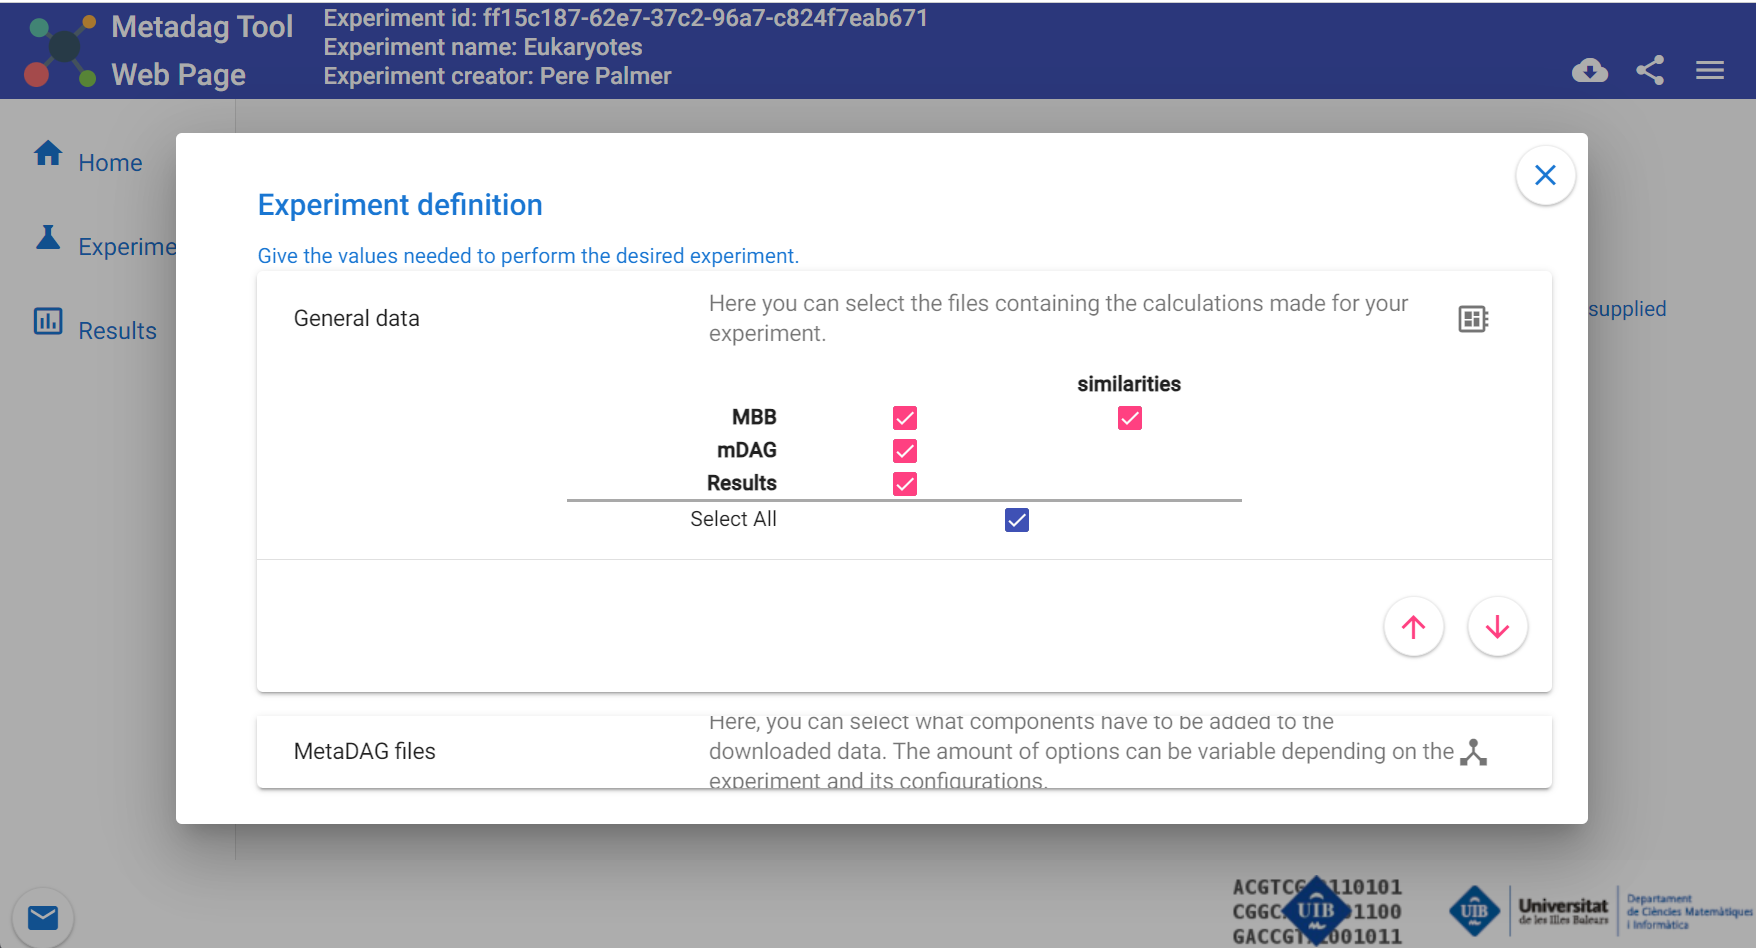
\includegraphics[width=1\textwidth,height=\textheight]{figures/screen_2.png}

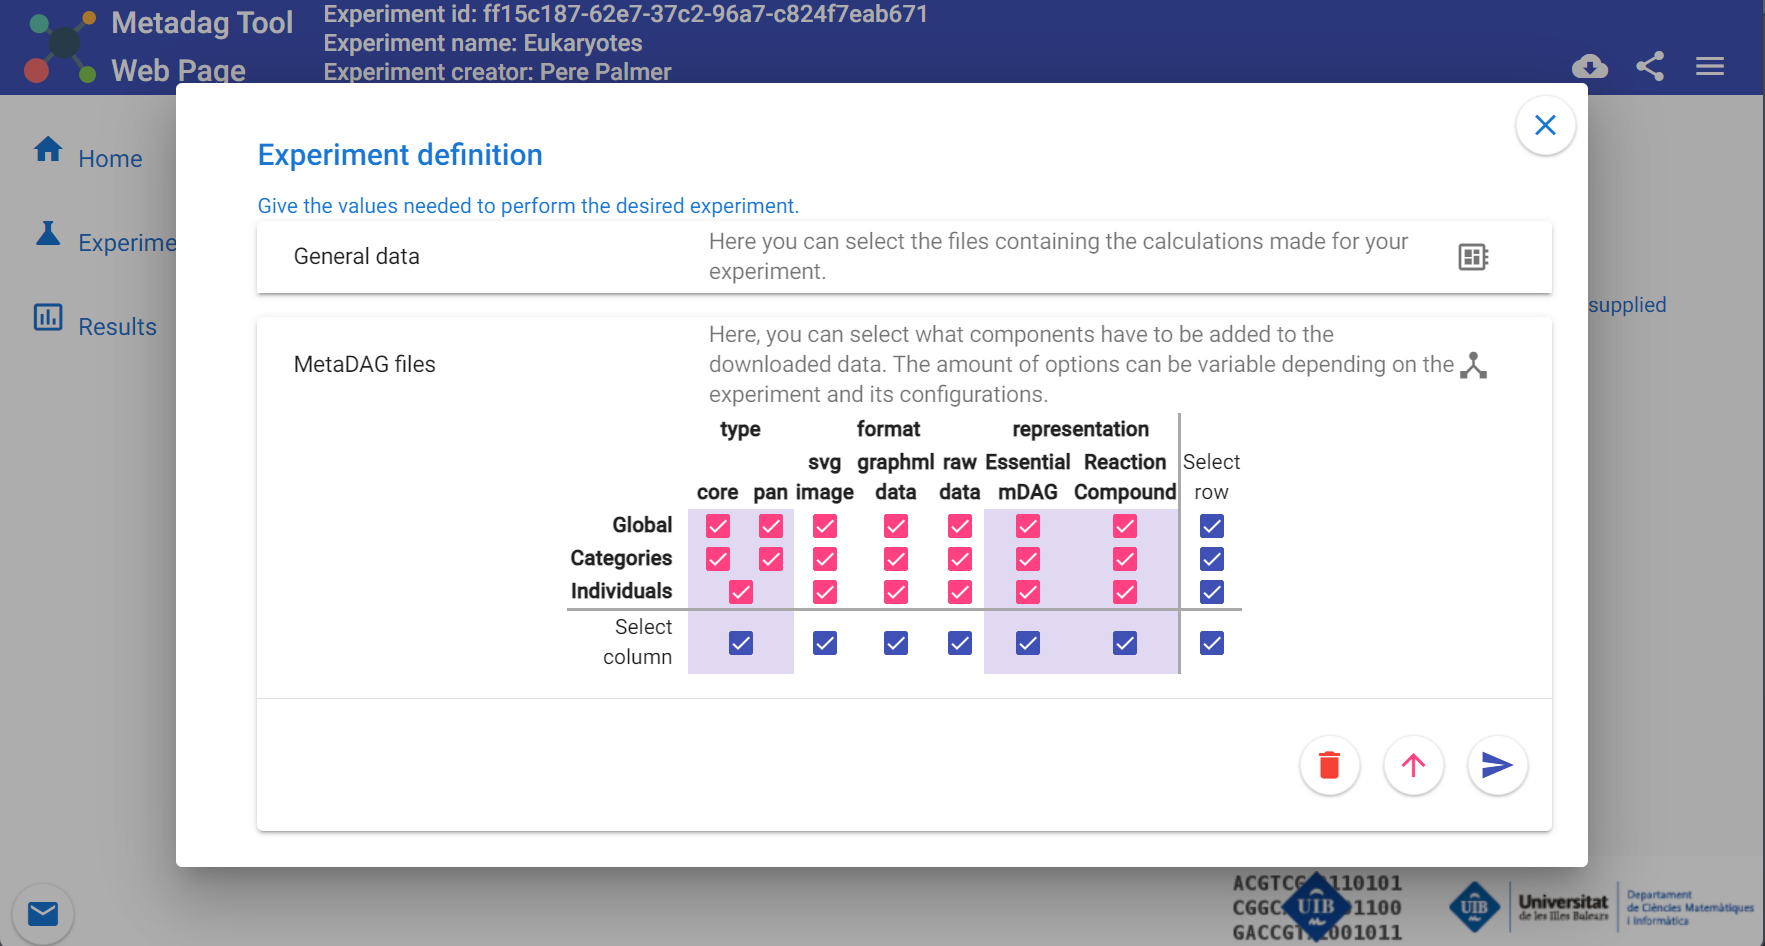
\includegraphics[width=1\textwidth,height=\textheight]{figures/screen_3.png}

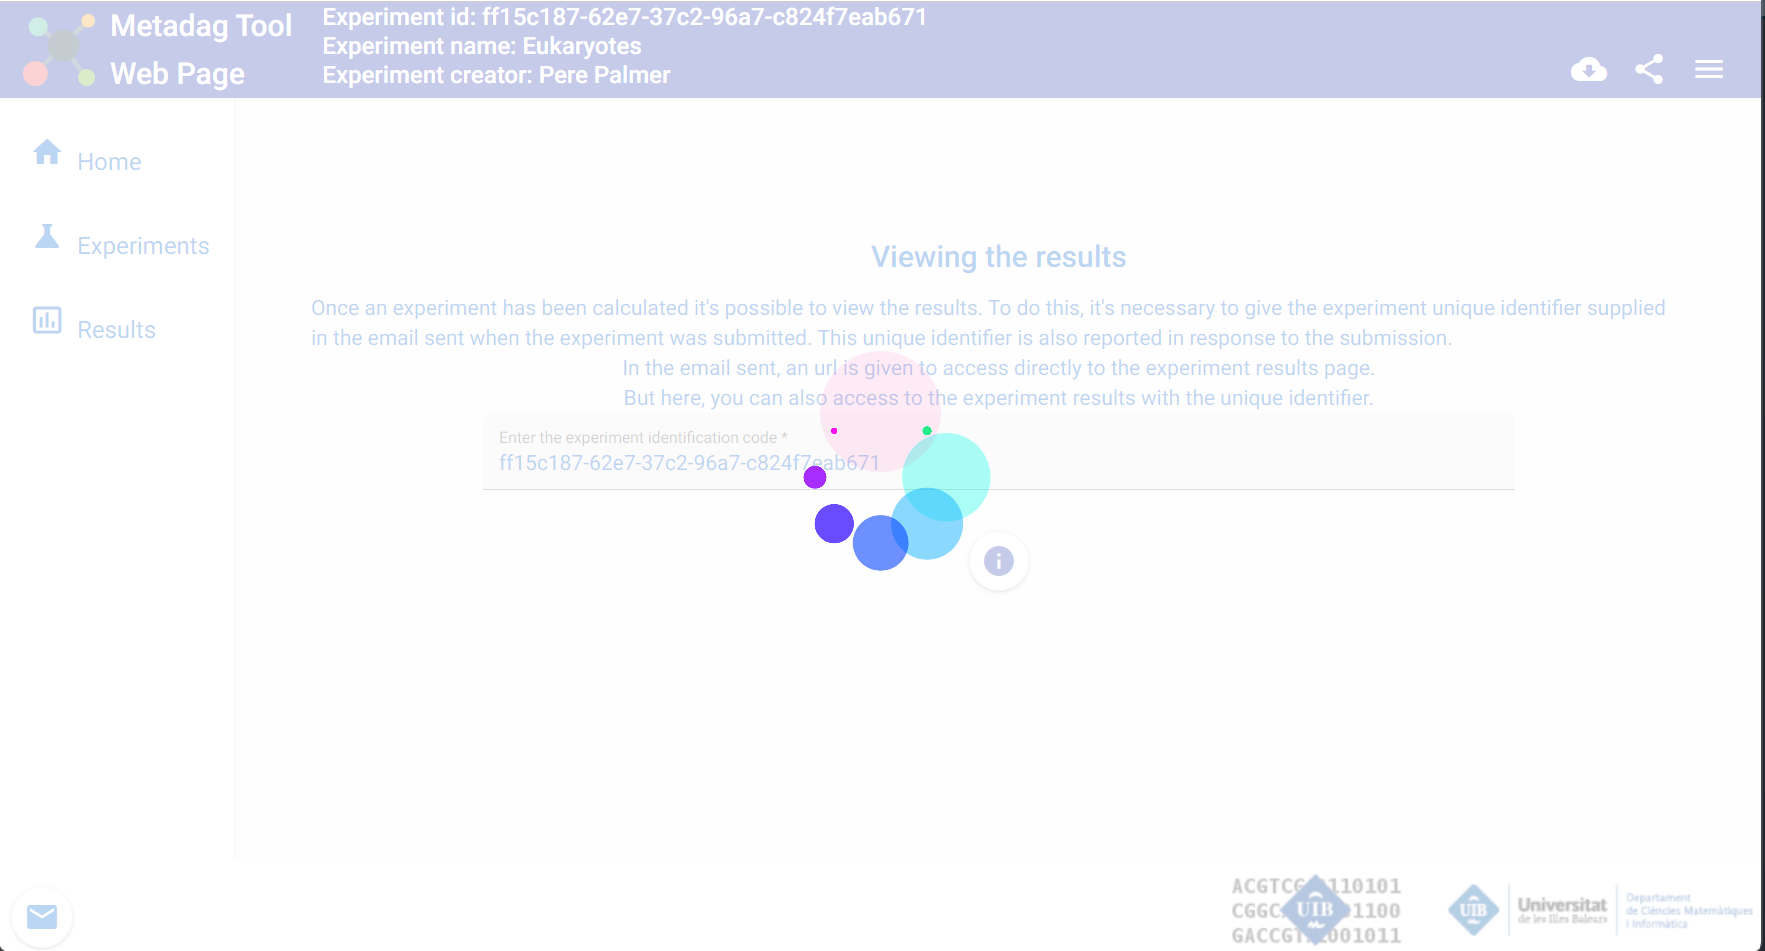
\includegraphics[width=1\textwidth,height=\textheight]{figures/screen_4.png}

\begin{Shaded}
\begin{Highlighting}[]
\NormalTok{experiment}\OtherTok{=}
  \StringTok{"result\_bb261b6e{-}95c6{-}3e39{-}b82b{-}b68eea80e30b"}
\NormalTok{path\_exp}\OtherTok{=}\FunctionTok{paste0}\NormalTok{(}\StringTok{"data/"}\NormalTok{,experiment,}\StringTok{"/data/"}\NormalTok{)}
\NormalTok{knitr}\SpecialCharTok{::}\FunctionTok{kable}\NormalTok{(}\FunctionTok{data.frame}\NormalTok{(}\AttributeTok{Directory\_files\_and\_folders=}\FunctionTok{dir}\NormalTok{(path\_exp),}
                        \AttributeTok{Type=}\FunctionTok{c}\NormalTok{(}\FunctionTok{rep}\NormalTok{(}\StringTok{"Data file"}\NormalTok{,}\DecValTok{2}\NormalTok{),}
                       \FunctionTok{rep}\NormalTok{(}\StringTok{"Directory"}\NormalTok{,}\DecValTok{2}\NormalTok{),}
                       \FunctionTok{rep}\NormalTok{(}\StringTok{"Data file"}\NormalTok{,}\DecValTok{5}\NormalTok{),}
                       \StringTok{"Directory"}\NormalTok{)))}
\end{Highlighting}
\end{Shaded}

\begin{tabular}{l|l}
\hline
Directory\_files\_and\_folders & Type\\
\hline
Different\_MBB.csv & Data file\\
\hline
Different\_mDAG.csv & Data file\\
\hline
Global & Directory\\
\hline
Individuals & Directory\\
\hline
Results.csv & Data file\\
\hline
Similarities\_MBB\_MSAMethod.csv & Data file\\
\hline
Similarities\_MBB\_MunkresMethod.csv & Data file\\
\hline
Similarities\_mDAG\_MSAMethod.csv & Data file\\
\hline
Similarities\_mDAG\_MunkresMethod.csv & Data file\\
\hline
TaxonomyLevels & Directory\\
\hline
\end{tabular}

\begin{Shaded}
\begin{Highlighting}[]
\NormalTok{MBB}\OtherTok{=}\FunctionTok{read\_csv}\NormalTok{(}\FunctionTok{paste0}\NormalTok{(path\_exp,}\StringTok{"Different\_MBB.csv"}\NormalTok{),}\AttributeTok{show\_col\_types =} \ConstantTok{FALSE}\NormalTok{)}
\NormalTok{mDAG}\OtherTok{=}\FunctionTok{read\_csv}\NormalTok{(}\FunctionTok{paste0}\NormalTok{(path\_exp,}\StringTok{"Different\_mDAG.csv"}\NormalTok{),}\AttributeTok{show\_col\_types =} \ConstantTok{FALSE}\NormalTok{)}
\NormalTok{Results}\OtherTok{=}\FunctionTok{read\_csv}\NormalTok{(}\FunctionTok{paste0}\NormalTok{(path\_exp,}\StringTok{"Results.csv"}\NormalTok{),}\AttributeTok{show\_col\_types =} \ConstantTok{FALSE}\NormalTok{)}
\FunctionTok{save}\NormalTok{(MBB,mDAG,Results,}\AttributeTok{file=}\StringTok{"MBB\_mDag\_Results.Rdata"}\NormalTok{)}
\end{Highlighting}
\end{Shaded}

\hypertarget{mbb}{%
\section{MBB}\label{mbb}}

In this experiment \texttt{MBB} is a table with 5112 rows and 4106
columns.

\begin{Shaded}
\begin{Highlighting}[]
\NormalTok{knitr}\SpecialCharTok{::}\FunctionTok{kable}\NormalTok{(MBB[}\DecValTok{1}\SpecialCharTok{:}\DecValTok{20}\NormalTok{,}\DecValTok{1}\SpecialCharTok{:}\DecValTok{100}\NormalTok{]) }\SpecialCharTok{\%\textgreater{}\%}   \FunctionTok{scroll\_box}\NormalTok{(}\AttributeTok{width =} \StringTok{"100\%"}\NormalTok{, }\AttributeTok{height =} \StringTok{"200px"}\NormalTok{)}
\end{Highlighting}
\end{Shaded}

\begin{tabular}{l|r|r|r|r|r|r|r|r|r|r|r|r|r|r|r|r|r|r|r|r|r|r|r|r|r|r|r|r|r|r|r|r|r|r|r|r|r|r|r|r|r|r|r|r|r|r|r|r|r|r|r|r|r|r|r|r|r|r|r|r|r|r|r|r|r|r|r|r|r|r|r|r|r|r|r|r|r|r|r|r|r|r|r|r|r|r|r|r|r|r|r|r|r|r|r|r|r|r|r}
\hline
MBB Id & natural & \#pathways & Protists & Fungi & Plants & Animals & Alveolates & Amoebozoa & Annelids & Arthropods & Ascomycetes & Basal angiosperms & Basidiomycetes & Brachiopodas & Cephalochordates & Choanoflagellates & Cnidarians & Cryptomonads & Echinoderms & Eudicots & Euglenozoa & Ferns & Flatworms & Green algae & Haptophyta & Hemichordates & Heterolobosea & Metamonada & Microsporidians & Mollusks & Monocots & Mosses & Nematodes & Placozoans & Poriferans & Red algae & Stramenopiles & Tunicates & Vertebrates & Acanthamoeba & Acanthus family & Amaranth family & Amborella family & Amphibians & Apicomplexans & Asparagus family & Banana family & Beech family & Birds & Bittersweet family & Buckthorn family & Caper family & Cartilaginous fishes & Chelicerates & Ciliates & Crustaceans & Cucumber family & Daisy family & Diatoms & Dictyostelia & Dinoflagellates & Diplomonads & Dothideomycetes & Entamoeba & Eurotiomycetes & Eustigmatophytes & Fishes & Ginger family & Grape family & Grass family & Insects & Kinetoplasts & Leotiomycetes & Lopseed family & Lotus family & Mallow family & Mammals & Mint family & Morning-glory family & Mulberry family & Mustard family & Myrtle family & Nightshade family & Olive family & Oomycetes & Orchid family & Palm family & Papaya family & Parsley family & Pea family & Pelagophytes & Pezizomycetes & Poppy family & Protea family & Reptiles & Rose family & Rue family & Saccharomycetes & Schizosaccharomycetes\\
\hline
0 & 0 & 0 & 0 & 0 & 0 & 0 & 0 & 0 & 0 & 0 & 0 & 0 & 0 & 0 & 0 & 0 & 0 & 0 & 0 & 0 & 0 & 0 & 0 & 0 & 0 & 0 & 0 & 0 & 0 & 0 & 0 & 0 & 0 & 0 & 0 & 0 & 0 & 0 & 0 & 0 & 0 & 0 & 0 & 0 & 0 & 0 & 0 & 0 & 0 & 0 & 0 & 0 & 0 & 0 & 0 & 0 & 0 & 0 & 0 & 0 & 0 & 0 & 0 & 0 & 0 & 0 & 0 & 0 & 0 & 0 & 0 & 0 & 0 & 0 & 0 & 0 & 0 & 0 & 0 & 0 & 0 & 0 & 0 & 0 & 0 & 0 & 0 & 0 & 0 & 0 & 0 & 0 & 0 & 0 & 0 & 0 & 0 & 0 & 0\\
\hline
0.0 & 0 & 0 & 0 & 0 & 0 & 0 & 0 & 0 & 0 & 0 & 0 & 0 & 0 & 0 & 0 & 0 & 0 & 0 & 0 & 0 & 0 & 0 & 0 & 0 & 0 & 0 & 0 & 0 & 0 & 0 & 0 & 0 & 0 & 0 & 0 & 0 & 0 & 0 & 0 & 0 & 0 & 0 & 0 & 0 & 0 & 0 & 0 & 0 & 0 & 0 & 0 & 0 & 0 & 0 & 0 & 0 & 0 & 0 & 0 & 0 & 0 & 0 & 0 & 0 & 0 & 0 & 0 & 0 & 0 & 0 & 0 & 0 & 0 & 0 & 0 & 0 & 0 & 0 & 0 & 0 & 0 & 0 & 0 & 0 & 0 & 0 & 0 & 0 & 0 & 0 & 0 & 0 & 0 & 0 & 0 & 0 & 0 & 0 & 0\\
\hline
0.0.0 & 1 & 1 & 1 & 0 & 0 & 0 & 0 & 0 & 0 & 0 & 0 & 0 & 0 & 0 & 0 & 0 & 0 & 0 & 0 & 0 & 0 & 0 & 0 & 0 & 0 & 0 & 0 & 0 & 0 & 0 & 0 & 0 & 0 & 0 & 0 & 0 & 1 & 0 & 0 & 0 & 0 & 0 & 0 & 0 & 0 & 0 & 0 & 0 & 0 & 0 & 0 & 0 & 0 & 0 & 0 & 0 & 0 & 0 & 0 & 0 & 0 & 0 & 0 & 0 & 0 & 0 & 0 & 0 & 0 & 0 & 0 & 0 & 0 & 0 & 0 & 0 & 0 & 0 & 0 & 0 & 0 & 0 & 0 & 0 & 1 & 0 & 0 & 0 & 0 & 0 & 0 & 0 & 0 & 0 & 0 & 0 & 0 & 0 & 0\\
\hline
0.0.0.0 & 1 & 1 & 1 & 0 & 0 & 0 & 0 & 0 & 0 & 0 & 0 & 0 & 0 & 0 & 0 & 0 & 0 & 0 & 0 & 0 & 0 & 0 & 0 & 0 & 0 & 0 & 0 & 0 & 0 & 0 & 0 & 0 & 0 & 0 & 0 & 0 & 1 & 0 & 0 & 0 & 0 & 0 & 0 & 0 & 0 & 0 & 0 & 0 & 0 & 0 & 0 & 0 & 0 & 0 & 0 & 0 & 0 & 0 & 0 & 0 & 0 & 0 & 0 & 0 & 0 & 0 & 0 & 0 & 0 & 0 & 0 & 0 & 0 & 0 & 0 & 0 & 0 & 0 & 0 & 0 & 0 & 0 & 0 & 0 & 1 & 0 & 0 & 0 & 0 & 0 & 0 & 0 & 0 & 0 & 0 & 0 & 0 & 0 & 0\\
\hline
0.0.1 & 1 & 1 & 1 & 0 & 0 & 0 & 0 & 0 & 0 & 0 & 0 & 0 & 0 & 0 & 0 & 0 & 0 & 0 & 0 & 0 & 0 & 0 & 0 & 0 & 0 & 0 & 0 & 0 & 0 & 0 & 0 & 0 & 0 & 0 & 0 & 0 & 1 & 0 & 0 & 0 & 0 & 0 & 0 & 0 & 0 & 0 & 0 & 0 & 0 & 0 & 0 & 0 & 0 & 0 & 0 & 0 & 0 & 0 & 0 & 0 & 0 & 0 & 0 & 0 & 0 & 0 & 0 & 0 & 0 & 0 & 0 & 0 & 0 & 0 & 0 & 0 & 0 & 0 & 0 & 0 & 0 & 0 & 0 & 0 & 1 & 0 & 0 & 0 & 0 & 0 & 0 & 0 & 0 & 0 & 0 & 0 & 0 & 0 & 0\\
\hline
0.0.1.0 & 1 & 86 & 2 & 77 & 1 & 6 & 1 & 0 & 0 & 5 & 57 & 0 & 20 & 0 & 0 & 0 & 0 & 0 & 0 & 0 & 0 & 0 & 0 & 0 & 1 & 0 & 0 & 0 & 0 & 0 & 0 & 0 & 0 & 0 & 1 & 1 & 0 & 0 & 0 & 0 & 0 & 0 & 0 & 0 & 0 & 0 & 0 & 0 & 0 & 0 & 0 & 0 & 0 & 0 & 0 & 5 & 0 & 0 & 0 & 0 & 1 & 0 & 11 & 0 & 14 & 0 & 0 & 0 & 0 & 0 & 0 & 0 & 5 & 0 & 0 & 0 & 0 & 0 & 0 & 0 & 0 & 0 & 0 & 0 & 0 & 0 & 0 & 0 & 0 & 0 & 0 & 0 & 0 & 0 & 0 & 0 & 0 & 1 & 0\\
\hline
0.0.1.1 & 1 & 86 & 2 & 77 & 1 & 6 & 1 & 0 & 0 & 5 & 57 & 0 & 20 & 0 & 0 & 0 & 0 & 0 & 0 & 0 & 0 & 0 & 0 & 0 & 1 & 0 & 0 & 0 & 0 & 0 & 0 & 0 & 0 & 0 & 1 & 1 & 0 & 0 & 0 & 0 & 0 & 0 & 0 & 0 & 0 & 0 & 0 & 0 & 0 & 0 & 0 & 0 & 0 & 0 & 0 & 5 & 0 & 0 & 0 & 0 & 1 & 0 & 11 & 0 & 14 & 0 & 0 & 0 & 0 & 0 & 0 & 0 & 5 & 0 & 0 & 0 & 0 & 0 & 0 & 0 & 0 & 0 & 0 & 0 & 0 & 0 & 0 & 0 & 0 & 0 & 0 & 0 & 0 & 0 & 0 & 0 & 0 & 1 & 0\\
\hline
0.0.1.2 & 1 & 15 & 15 & 0 & 0 & 0 & 12 & 0 & 0 & 0 & 0 & 0 & 0 & 0 & 0 & 0 & 0 & 0 & 0 & 0 & 0 & 0 & 0 & 0 & 0 & 0 & 0 & 0 & 0 & 0 & 0 & 0 & 0 & 0 & 0 & 0 & 3 & 0 & 0 & 0 & 0 & 0 & 0 & 0 & 12 & 0 & 0 & 0 & 0 & 0 & 0 & 0 & 0 & 0 & 0 & 0 & 0 & 0 & 1 & 0 & 0 & 0 & 0 & 0 & 0 & 0 & 0 & 0 & 0 & 0 & 0 & 0 & 0 & 0 & 0 & 0 & 0 & 0 & 0 & 0 & 0 & 0 & 0 & 0 & 1 & 0 & 0 & 0 & 0 & 0 & 1 & 0 & 0 & 0 & 0 & 0 & 0 & 0 & 0\\
\hline
0.0.1.3 & 1 & 5 & 5 & 0 & 0 & 0 & 0 & 4 & 0 & 0 & 0 & 0 & 0 & 0 & 0 & 0 & 0 & 0 & 0 & 0 & 0 & 0 & 0 & 0 & 0 & 0 & 1 & 0 & 0 & 0 & 0 & 0 & 0 & 0 & 0 & 0 & 0 & 0 & 0 & 1 & 0 & 0 & 0 & 0 & 0 & 0 & 0 & 0 & 0 & 0 & 0 & 0 & 0 & 0 & 0 & 0 & 0 & 0 & 0 & 3 & 0 & 0 & 0 & 0 & 0 & 0 & 0 & 0 & 0 & 0 & 0 & 0 & 0 & 0 & 0 & 0 & 0 & 0 & 0 & 0 & 0 & 0 & 0 & 0 & 0 & 0 & 0 & 0 & 0 & 0 & 0 & 0 & 0 & 0 & 0 & 0 & 0 & 0 & 0\\
\hline
0.0.1.4 & 0 & 0 & 0 & 0 & 0 & 0 & 0 & 0 & 0 & 0 & 0 & 0 & 0 & 0 & 0 & 0 & 0 & 0 & 0 & 0 & 0 & 0 & 0 & 0 & 0 & 0 & 0 & 0 & 0 & 0 & 0 & 0 & 0 & 0 & 0 & 0 & 0 & 0 & 0 & 0 & 0 & 0 & 0 & 0 & 0 & 0 & 0 & 0 & 0 & 0 & 0 & 0 & 0 & 0 & 0 & 0 & 0 & 0 & 0 & 0 & 0 & 0 & 0 & 0 & 0 & 0 & 0 & 0 & 0 & 0 & 0 & 0 & 0 & 0 & 0 & 0 & 0 & 0 & 0 & 0 & 0 & 0 & 0 & 0 & 0 & 0 & 0 & 0 & 0 & 0 & 0 & 0 & 0 & 0 & 0 & 0 & 0 & 0 & 0\\
\hline
0.0.1.4.0 & 1 & 609 & 14 & 128 & 128 & 339 & 1 & 3 & 1 & 8 & 93 & 2 & 35 & 1 & 2 & 2 & 4 & 0 & 3 & 98 & 0 & 1 & 3 & 3 & 1 & 1 & 1 & 1 & 0 & 14 & 23 & 1 & 2 & 0 & 1 & 0 & 5 & 2 & 297 & 0 & 1 & 3 & 1 & 6 & 0 & 1 & 1 & 2 & 53 & 1 & 1 & 1 & 0 & 2 & 0 & 0 & 7 & 4 & 3 & 0 & 1 & 0 & 11 & 3 & 23 & 1 & 89 & 1 & 2 & 16 & 6 & 0 & 5 & 1 & 1 & 5 & 128 & 1 & 2 & 1 & 9 & 1 & 9 & 1 & 0 & 2 & 2 & 1 & 1 & 17 & 1 & 1 & 1 & 2 & 21 & 8 & 2 & 21 & 1\\
\hline
0.0.1.4.1 & 1 & 609 & 14 & 128 & 128 & 339 & 1 & 3 & 1 & 8 & 93 & 2 & 35 & 1 & 2 & 2 & 4 & 0 & 3 & 98 & 0 & 1 & 3 & 3 & 1 & 1 & 1 & 1 & 0 & 14 & 23 & 1 & 2 & 0 & 1 & 0 & 5 & 2 & 297 & 0 & 1 & 3 & 1 & 6 & 0 & 1 & 1 & 2 & 53 & 1 & 1 & 1 & 0 & 2 & 0 & 0 & 7 & 4 & 3 & 0 & 1 & 0 & 11 & 3 & 23 & 1 & 89 & 1 & 2 & 16 & 6 & 0 & 5 & 1 & 1 & 5 & 128 & 1 & 2 & 1 & 9 & 1 & 9 & 1 & 0 & 2 & 2 & 1 & 1 & 17 & 1 & 1 & 1 & 2 & 21 & 8 & 2 & 21 & 1\\
\hline
0.0.1.4.2 & 1 & 322 & 6 & 92 & 133 & 91 & 1 & 0 & 0 & 61 & 62 & 2 & 30 & 1 & 2 & 1 & 8 & 0 & 2 & 98 & 0 & 1 & 0 & 7 & 1 & 1 & 1 & 0 & 0 & 13 & 23 & 1 & 0 & 0 & 0 & 1 & 2 & 2 & 1 & 0 & 1 & 3 & 1 & 0 & 0 & 1 & 1 & 2 & 0 & 1 & 1 & 1 & 0 & 1 & 0 & 11 & 7 & 4 & 1 & 0 & 1 & 0 & 11 & 0 & 14 & 1 & 0 & 1 & 2 & 16 & 49 & 0 & 5 & 1 & 1 & 5 & 1 & 1 & 2 & 1 & 9 & 1 & 9 & 1 & 0 & 2 & 2 & 1 & 1 & 17 & 0 & 1 & 1 & 2 & 0 & 8 & 2 & 0 & 0\\
\hline
0.0.1.4.3 & 1 & 322 & 6 & 92 & 133 & 91 & 1 & 0 & 0 & 61 & 62 & 2 & 30 & 1 & 2 & 1 & 8 & 0 & 2 & 98 & 0 & 1 & 0 & 7 & 1 & 1 & 1 & 0 & 0 & 13 & 23 & 1 & 0 & 0 & 0 & 1 & 2 & 2 & 1 & 0 & 1 & 3 & 1 & 0 & 0 & 1 & 1 & 2 & 0 & 1 & 1 & 1 & 0 & 1 & 0 & 11 & 7 & 4 & 1 & 0 & 1 & 0 & 11 & 0 & 14 & 1 & 0 & 1 & 2 & 16 & 49 & 0 & 5 & 1 & 1 & 5 & 1 & 1 & 2 & 1 & 9 & 1 & 9 & 1 & 0 & 2 & 2 & 1 & 1 & 17 & 0 & 1 & 1 & 2 & 0 & 8 & 2 & 0 & 0\\
\hline
0.0.1.4.4 & 1 & 1 & 0 & 0 & 1 & 0 & 0 & 0 & 0 & 0 & 0 & 0 & 0 & 0 & 0 & 0 & 0 & 0 & 0 & 0 & 0 & 0 & 0 & 0 & 0 & 0 & 0 & 0 & 0 & 0 & 0 & 0 & 0 & 0 & 0 & 1 & 0 & 0 & 0 & 0 & 0 & 0 & 0 & 0 & 0 & 0 & 0 & 0 & 0 & 0 & 0 & 0 & 0 & 0 & 0 & 0 & 0 & 0 & 0 & 0 & 0 & 0 & 0 & 0 & 0 & 0 & 0 & 0 & 0 & 0 & 0 & 0 & 0 & 0 & 0 & 0 & 0 & 0 & 0 & 0 & 0 & 0 & 0 & 0 & 0 & 0 & 0 & 0 & 0 & 0 & 0 & 0 & 0 & 0 & 0 & 0 & 0 & 0 & 0\\
\hline
0.0.1.4.5 & 1 & 1 & 1 & 0 & 0 & 0 & 0 & 1 & 0 & 0 & 0 & 0 & 0 & 0 & 0 & 0 & 0 & 0 & 0 & 0 & 0 & 0 & 0 & 0 & 0 & 0 & 0 & 0 & 0 & 0 & 0 & 0 & 0 & 0 & 0 & 0 & 0 & 0 & 0 & 0 & 0 & 0 & 0 & 0 & 0 & 0 & 0 & 0 & 0 & 0 & 0 & 0 & 0 & 0 & 0 & 0 & 0 & 0 & 0 & 1 & 0 & 0 & 0 & 0 & 0 & 0 & 0 & 0 & 0 & 0 & 0 & 0 & 0 & 0 & 0 & 0 & 0 & 0 & 0 & 0 & 0 & 0 & 0 & 0 & 0 & 0 & 0 & 0 & 0 & 0 & 0 & 0 & 0 & 0 & 0 & 0 & 0 & 0 & 0\\
\hline
0.0.1.5 & 0 & 0 & 0 & 0 & 0 & 0 & 0 & 0 & 0 & 0 & 0 & 0 & 0 & 0 & 0 & 0 & 0 & 0 & 0 & 0 & 0 & 0 & 0 & 0 & 0 & 0 & 0 & 0 & 0 & 0 & 0 & 0 & 0 & 0 & 0 & 0 & 0 & 0 & 0 & 0 & 0 & 0 & 0 & 0 & 0 & 0 & 0 & 0 & 0 & 0 & 0 & 0 & 0 & 0 & 0 & 0 & 0 & 0 & 0 & 0 & 0 & 0 & 0 & 0 & 0 & 0 & 0 & 0 & 0 & 0 & 0 & 0 & 0 & 0 & 0 & 0 & 0 & 0 & 0 & 0 & 0 & 0 & 0 & 0 & 0 & 0 & 0 & 0 & 0 & 0 & 0 & 0 & 0 & 0 & 0 & 0 & 0 & 0 & 0\\
\hline
0.0.1.5.0 & 1 & 5 & 5 & 0 & 0 & 0 & 0 & 4 & 0 & 0 & 0 & 0 & 0 & 0 & 0 & 0 & 0 & 0 & 0 & 0 & 0 & 0 & 0 & 0 & 0 & 0 & 1 & 0 & 0 & 0 & 0 & 0 & 0 & 0 & 0 & 0 & 0 & 0 & 0 & 1 & 0 & 0 & 0 & 0 & 0 & 0 & 0 & 0 & 0 & 0 & 0 & 0 & 0 & 0 & 0 & 0 & 0 & 0 & 0 & 3 & 0 & 0 & 0 & 0 & 0 & 0 & 0 & 0 & 0 & 0 & 0 & 0 & 0 & 0 & 0 & 0 & 0 & 0 & 0 & 0 & 0 & 0 & 0 & 0 & 0 & 0 & 0 & 0 & 0 & 0 & 0 & 0 & 0 & 0 & 0 & 0 & 0 & 0 & 0\\
\hline
0.0.2 & 1 & 1 & 1 & 0 & 0 & 0 & 0 & 0 & 0 & 0 & 0 & 0 & 0 & 0 & 0 & 0 & 0 & 0 & 0 & 0 & 0 & 0 & 0 & 0 & 0 & 0 & 0 & 0 & 0 & 0 & 0 & 0 & 0 & 0 & 0 & 0 & 1 & 0 & 0 & 0 & 0 & 0 & 0 & 0 & 0 & 0 & 0 & 0 & 0 & 0 & 0 & 0 & 0 & 0 & 0 & 0 & 0 & 0 & 0 & 0 & 0 & 0 & 0 & 0 & 0 & 0 & 0 & 0 & 0 & 0 & 0 & 0 & 0 & 0 & 0 & 0 & 0 & 0 & 0 & 0 & 0 & 0 & 0 & 0 & 1 & 0 & 0 & 0 & 0 & 0 & 0 & 0 & 0 & 0 & 0 & 0 & 0 & 0 & 0\\
\hline
0.0.3 & 1 & 1 & 1 & 0 & 0 & 0 & 0 & 1 & 0 & 0 & 0 & 0 & 0 & 0 & 0 & 0 & 0 & 0 & 0 & 0 & 0 & 0 & 0 & 0 & 0 & 0 & 0 & 0 & 0 & 0 & 0 & 0 & 0 & 0 & 0 & 0 & 0 & 0 & 0 & 1 & 0 & 0 & 0 & 0 & 0 & 0 & 0 & 0 & 0 & 0 & 0 & 0 & 0 & 0 & 0 & 0 & 0 & 0 & 0 & 0 & 0 & 0 & 0 & 0 & 0 & 0 & 0 & 0 & 0 & 0 & 0 & 0 & 0 & 0 & 0 & 0 & 0 & 0 & 0 & 0 & 0 & 0 & 0 & 0 & 0 & 0 & 0 & 0 & 0 & 0 & 0 & 0 & 0 & 0 & 0 & 0 & 0 & 0 & 0\\
\hline
\end{tabular}

\hypertarget{mdag}{%
\section{mDAG}\label{mdag}}

Abstract/unique mDAG's in this experiment

\begin{Shaded}
\begin{Highlighting}[]
\FunctionTok{dim}\NormalTok{(mDAG)}
\end{Highlighting}
\end{Shaded}

\begin{verbatim}
[1]  884 5224
\end{verbatim}

\begin{Shaded}
\begin{Highlighting}[]
\FunctionTok{kable}\NormalTok{(mDAG[}\DecValTok{1}\SpecialCharTok{:}\DecValTok{20}\NormalTok{,}\DecValTok{1}\SpecialCharTok{:}\DecValTok{100}\NormalTok{]) }\SpecialCharTok{\%\textgreater{}\%}   \FunctionTok{scroll\_box}\NormalTok{(}\AttributeTok{width =} \StringTok{"100\%"}\NormalTok{, }\AttributeTok{height =} \StringTok{"200px"}\NormalTok{)}
\end{Highlighting}
\end{Shaded}

\begin{tabular}{l|r|r|r|r|r|r|r|r|r|r|r|r|r|r|r|r|r|r|r|r|r|r|r|r|r|r|r|r|r|r|r|r|r|r|r|r|r|r|r|r|r|r|r|r|r|r|r|r|r|r|r|r|r|r|r|r|r|r|r|r|r|r|r|r|r|r|r|r|r|r|r|r|r|r|r|r|r|r|r|r|r|r|r|r|r|r|r|r|r|r|r|r|r|r|r|r|r|r|r}
\hline
mDAG Id & \#Categories & Animals & Plants & Fungi & Protists & Alveolates & Amoebozoa & Annelids & Arthropods & Ascomycetes & Basal angiosperms & Basidiomycetes & Brachiopodas & Cephalochordates & Choanoflagellates & Cnidarians & Cryptomonads & Echinoderms & Eudicots & Euglenozoa & Ferns & Flatworms & Green algae & Haptophyta & Hemichordates & Heterolobosea & Metamonada & Microsporidians & Mollusks & Monocots & Mosses & Nematodes & Placozoans & Poriferans & Red algae & Stramenopiles & Tunicates & Vertebrates & Acanthamoeba & Acanthus family & Amaranth family & Amborella family & Amphibians & Apicomplexans & Asparagus family & Banana family & Beech family & Birds & Bittersweet family & Buckthorn family & Caper family & Cartilaginous fishes & Chelicerates & Ciliates & Crustaceans & Cucumber family & Daisy family & Diatoms & Dictyostelia & Dinoflagellates & Diplomonads & Dothideomycetes & Entamoeba & Eurotiomycetes & Eustigmatophytes & Fishes & Ginger family & Grape family & Grass family & Insects & Kinetoplasts & Leotiomycetes & Lopseed family & Lotus family & Mallow family & Mammals & Mint family & Morning-glory family & Mulberry family & Mustard family & Myrtle family & Nightshade family & Olive family & Oomycetes & Orchid family & Palm family & Papaya family & Parsley family & Pea family & Pelagophytes & Pezizomycetes & Poppy family & Protea family & Reptiles & Rose family & Rue family & Saccharomycetes & Schizosaccharomycetes & Sesame family\\
\hline
0001 & 3 & 1 & 0 & 0 & 0 & 0 & 0 & 0 & 0 & 0 & 0 & 0 & 0 & 0 & 0 & 0 & 0 & 0 & 0 & 0 & 0 & 0 & 0 & 0 & 0 & 0 & 0 & 0 & 0 & 0 & 0 & 0 & 0 & 0 & 0 & 0 & 0 & 1 & 0 & 0 & 0 & 0 & 0 & 0 & 0 & 0 & 0 & 1 & 0 & 0 & 0 & 0 & 0 & 0 & 0 & 0 & 0 & 0 & 0 & 0 & 0 & 0 & 0 & 0 & 0 & 0 & 0 & 0 & 0 & 0 & 0 & 0 & 0 & 0 & 0 & 0 & 0 & 0 & 0 & 0 & 0 & 0 & 0 & 0 & 0 & 0 & 0 & 0 & 0 & 0 & 0 & 0 & 0 & 0 & 0 & 0 & 0 & 0 & 0\\
\hline
0002 & 2 & 0 & 0 & 1 & 0 & 0 & 0 & 0 & 0 & 0 & 0 & 1 & 0 & 0 & 0 & 0 & 0 & 0 & 0 & 0 & 0 & 0 & 0 & 0 & 0 & 0 & 0 & 0 & 0 & 0 & 0 & 0 & 0 & 0 & 0 & 0 & 0 & 0 & 0 & 0 & 0 & 0 & 0 & 0 & 0 & 0 & 0 & 0 & 0 & 0 & 0 & 0 & 0 & 0 & 0 & 0 & 0 & 0 & 0 & 0 & 0 & 0 & 0 & 0 & 0 & 0 & 0 & 0 & 0 & 0 & 0 & 0 & 0 & 0 & 0 & 0 & 0 & 0 & 0 & 0 & 0 & 0 & 0 & 0 & 0 & 0 & 0 & 0 & 0 & 0 & 0 & 0 & 0 & 0 & 0 & 0 & 0 & 0 & 0\\
\hline
0003 & 2 & 1 & 0 & 0 & 0 & 0 & 0 & 0 & 0 & 0 & 0 & 0 & 0 & 0 & 0 & 0 & 0 & 0 & 0 & 0 & 0 & 1 & 0 & 0 & 0 & 0 & 0 & 0 & 0 & 0 & 0 & 0 & 0 & 0 & 0 & 0 & 0 & 0 & 0 & 0 & 0 & 0 & 0 & 0 & 0 & 0 & 0 & 0 & 0 & 0 & 0 & 0 & 0 & 0 & 0 & 0 & 0 & 0 & 0 & 0 & 0 & 0 & 0 & 0 & 0 & 0 & 0 & 0 & 0 & 0 & 0 & 0 & 0 & 0 & 0 & 0 & 0 & 0 & 0 & 0 & 0 & 0 & 0 & 0 & 0 & 0 & 0 & 0 & 0 & 0 & 0 & 0 & 0 & 0 & 0 & 0 & 0 & 0 & 0\\
\hline
0004 & 3 & 1 & 0 & 0 & 0 & 0 & 0 & 0 & 0 & 0 & 0 & 0 & 0 & 0 & 0 & 0 & 0 & 0 & 0 & 0 & 0 & 0 & 0 & 0 & 0 & 0 & 0 & 0 & 0 & 0 & 0 & 0 & 0 & 0 & 0 & 0 & 0 & 1 & 0 & 0 & 0 & 0 & 0 & 0 & 0 & 0 & 0 & 1 & 0 & 0 & 0 & 0 & 0 & 0 & 0 & 0 & 0 & 0 & 0 & 0 & 0 & 0 & 0 & 0 & 0 & 0 & 0 & 0 & 0 & 0 & 0 & 0 & 0 & 0 & 0 & 0 & 0 & 0 & 0 & 0 & 0 & 0 & 0 & 0 & 0 & 0 & 0 & 0 & 0 & 0 & 0 & 0 & 0 & 0 & 0 & 0 & 0 & 0 & 0\\
\hline
0005 & 3 & 1 & 0 & 0 & 0 & 0 & 0 & 0 & 0 & 0 & 0 & 0 & 0 & 0 & 0 & 0 & 0 & 0 & 0 & 0 & 0 & 0 & 0 & 0 & 0 & 0 & 0 & 0 & 0 & 0 & 0 & 0 & 0 & 0 & 0 & 0 & 0 & 1 & 0 & 0 & 0 & 0 & 0 & 0 & 0 & 0 & 0 & 0 & 0 & 0 & 0 & 0 & 0 & 0 & 0 & 0 & 0 & 0 & 0 & 0 & 0 & 0 & 0 & 0 & 0 & 1 & 0 & 0 & 0 & 0 & 0 & 0 & 0 & 0 & 0 & 0 & 0 & 0 & 0 & 0 & 0 & 0 & 0 & 0 & 0 & 0 & 0 & 0 & 0 & 0 & 0 & 0 & 0 & 0 & 0 & 0 & 0 & 0 & 0\\
\hline
0006 & 3 & 0 & 1 & 0 & 0 & 0 & 0 & 0 & 0 & 0 & 0 & 0 & 0 & 0 & 0 & 0 & 0 & 0 & 1 & 0 & 0 & 0 & 0 & 0 & 0 & 0 & 0 & 0 & 0 & 0 & 0 & 0 & 0 & 0 & 0 & 0 & 0 & 0 & 0 & 0 & 0 & 0 & 0 & 0 & 0 & 0 & 0 & 0 & 0 & 0 & 0 & 0 & 0 & 0 & 0 & 0 & 0 & 0 & 0 & 0 & 0 & 0 & 0 & 0 & 0 & 0 & 0 & 0 & 0 & 0 & 0 & 0 & 0 & 0 & 0 & 0 & 0 & 0 & 0 & 0 & 1 & 0 & 0 & 0 & 0 & 0 & 0 & 0 & 0 & 0 & 0 & 0 & 0 & 0 & 0 & 0 & 0 & 0 & 0\\
\hline
0007 & 2 & 0 & 1 & 0 & 0 & 0 & 0 & 0 & 0 & 0 & 0 & 0 & 0 & 0 & 0 & 0 & 0 & 0 & 0 & 0 & 0 & 0 & 0 & 0 & 0 & 0 & 0 & 0 & 0 & 0 & 0 & 0 & 0 & 0 & 1 & 0 & 0 & 0 & 0 & 0 & 0 & 0 & 0 & 0 & 0 & 0 & 0 & 0 & 0 & 0 & 0 & 0 & 0 & 0 & 0 & 0 & 0 & 0 & 0 & 0 & 0 & 0 & 0 & 0 & 0 & 0 & 0 & 0 & 0 & 0 & 0 & 0 & 0 & 0 & 0 & 0 & 0 & 0 & 0 & 0 & 0 & 0 & 0 & 0 & 0 & 0 & 0 & 0 & 0 & 0 & 0 & 0 & 0 & 0 & 0 & 0 & 0 & 0 & 0\\
\hline
0008 & 3 & 0 & 1 & 0 & 0 & 0 & 0 & 0 & 0 & 0 & 0 & 0 & 0 & 0 & 0 & 0 & 0 & 0 & 0 & 0 & 0 & 0 & 0 & 0 & 0 & 0 & 0 & 0 & 0 & 1 & 0 & 0 & 0 & 0 & 0 & 0 & 0 & 0 & 0 & 0 & 0 & 0 & 0 & 0 & 0 & 0 & 0 & 0 & 0 & 0 & 0 & 0 & 0 & 0 & 0 & 0 & 0 & 0 & 0 & 0 & 0 & 0 & 0 & 0 & 0 & 0 & 0 & 0 & 0 & 0 & 0 & 0 & 0 & 0 & 0 & 0 & 0 & 0 & 0 & 0 & 0 & 0 & 0 & 0 & 0 & 1 & 0 & 0 & 0 & 0 & 0 & 0 & 0 & 0 & 0 & 0 & 0 & 0 & 0\\
\hline
0009 & 3 & 0 & 1 & 0 & 0 & 0 & 0 & 0 & 0 & 0 & 0 & 0 & 0 & 0 & 0 & 0 & 0 & 0 & 1 & 0 & 0 & 0 & 0 & 0 & 0 & 0 & 0 & 0 & 0 & 0 & 0 & 0 & 0 & 0 & 0 & 0 & 0 & 0 & 0 & 0 & 0 & 0 & 0 & 0 & 0 & 0 & 0 & 0 & 0 & 0 & 0 & 0 & 0 & 0 & 0 & 0 & 0 & 0 & 0 & 0 & 0 & 0 & 0 & 0 & 0 & 0 & 0 & 0 & 0 & 0 & 0 & 0 & 1 & 0 & 0 & 0 & 0 & 0 & 0 & 0 & 0 & 0 & 0 & 0 & 0 & 0 & 0 & 0 & 0 & 0 & 0 & 0 & 0 & 0 & 0 & 0 & 0 & 0 & 0\\
\hline
0010 & 3 & 1 & 0 & 0 & 0 & 0 & 0 & 0 & 0 & 0 & 0 & 0 & 0 & 0 & 0 & 0 & 0 & 0 & 0 & 0 & 0 & 0 & 0 & 0 & 0 & 0 & 0 & 0 & 0 & 0 & 0 & 0 & 0 & 0 & 0 & 0 & 0 & 1 & 0 & 0 & 0 & 0 & 0 & 0 & 0 & 0 & 0 & 1 & 0 & 0 & 0 & 0 & 0 & 0 & 0 & 0 & 0 & 0 & 0 & 0 & 0 & 0 & 0 & 0 & 0 & 0 & 0 & 0 & 0 & 0 & 0 & 0 & 0 & 0 & 0 & 0 & 0 & 0 & 0 & 0 & 0 & 0 & 0 & 0 & 0 & 0 & 0 & 0 & 0 & 0 & 0 & 0 & 0 & 0 & 0 & 0 & 0 & 0 & 0\\
\hline
0011 & 3 & 1 & 0 & 0 & 0 & 0 & 0 & 0 & 0 & 0 & 0 & 0 & 0 & 0 & 0 & 0 & 0 & 0 & 0 & 0 & 0 & 0 & 0 & 0 & 0 & 0 & 0 & 0 & 0 & 0 & 0 & 0 & 0 & 0 & 0 & 0 & 0 & 1 & 0 & 0 & 0 & 0 & 0 & 0 & 0 & 0 & 0 & 1 & 0 & 0 & 0 & 0 & 0 & 0 & 0 & 0 & 0 & 0 & 0 & 0 & 0 & 0 & 0 & 0 & 0 & 0 & 0 & 0 & 0 & 0 & 0 & 0 & 0 & 0 & 0 & 0 & 0 & 0 & 0 & 0 & 0 & 0 & 0 & 0 & 0 & 0 & 0 & 0 & 0 & 0 & 0 & 0 & 0 & 0 & 0 & 0 & 0 & 0 & 0\\
\hline
0012 & 3 & 0 & 0 & 0 & 1 & 0 & 0 & 0 & 0 & 0 & 0 & 0 & 0 & 0 & 0 & 0 & 0 & 0 & 0 & 0 & 0 & 0 & 0 & 0 & 0 & 0 & 1 & 0 & 0 & 0 & 0 & 0 & 0 & 0 & 0 & 0 & 0 & 0 & 0 & 0 & 0 & 0 & 0 & 0 & 0 & 0 & 0 & 0 & 0 & 0 & 0 & 0 & 0 & 0 & 0 & 0 & 0 & 0 & 0 & 0 & 1 & 0 & 0 & 0 & 0 & 0 & 0 & 0 & 0 & 0 & 0 & 0 & 0 & 0 & 0 & 0 & 0 & 0 & 0 & 0 & 0 & 0 & 0 & 0 & 0 & 0 & 0 & 0 & 0 & 0 & 0 & 0 & 0 & 0 & 0 & 0 & 0 & 0 & 0\\
\hline
0013 & 3 & 1 & 0 & 0 & 0 & 0 & 0 & 0 & 0 & 0 & 0 & 0 & 0 & 0 & 0 & 0 & 0 & 0 & 0 & 0 & 0 & 0 & 0 & 0 & 0 & 0 & 0 & 0 & 0 & 0 & 0 & 0 & 0 & 0 & 0 & 0 & 0 & 1 & 0 & 0 & 0 & 0 & 0 & 0 & 0 & 0 & 0 & 1 & 0 & 0 & 0 & 0 & 0 & 0 & 0 & 0 & 0 & 0 & 0 & 0 & 0 & 0 & 0 & 0 & 0 & 0 & 0 & 0 & 0 & 0 & 0 & 0 & 0 & 0 & 0 & 0 & 0 & 0 & 0 & 0 & 0 & 0 & 0 & 0 & 0 & 0 & 0 & 0 & 0 & 0 & 0 & 0 & 0 & 0 & 0 & 0 & 0 & 0 & 0\\
\hline
0014 & 3 & 0 & 0 & 0 & 1 & 1 & 0 & 0 & 0 & 0 & 0 & 0 & 0 & 0 & 0 & 0 & 0 & 0 & 0 & 0 & 0 & 0 & 0 & 0 & 0 & 0 & 0 & 0 & 0 & 0 & 0 & 0 & 0 & 0 & 0 & 0 & 0 & 0 & 0 & 0 & 0 & 0 & 0 & 0 & 0 & 0 & 0 & 0 & 0 & 0 & 0 & 0 & 0 & 1 & 0 & 0 & 0 & 0 & 0 & 0 & 0 & 0 & 0 & 0 & 0 & 0 & 0 & 0 & 0 & 0 & 0 & 0 & 0 & 0 & 0 & 0 & 0 & 0 & 0 & 0 & 0 & 0 & 0 & 0 & 0 & 0 & 0 & 0 & 0 & 0 & 0 & 0 & 0 & 0 & 0 & 0 & 0 & 0 & 0\\
\hline
0015 & 2 & 0 & 0 & 1 & 0 & 0 & 0 & 0 & 0 & 0 & 0 & 0 & 0 & 0 & 0 & 0 & 0 & 0 & 0 & 0 & 0 & 0 & 0 & 0 & 0 & 0 & 0 & 1 & 0 & 0 & 0 & 0 & 0 & 0 & 0 & 0 & 0 & 0 & 0 & 0 & 0 & 0 & 0 & 0 & 0 & 0 & 0 & 0 & 0 & 0 & 0 & 0 & 0 & 0 & 0 & 0 & 0 & 0 & 0 & 0 & 0 & 0 & 0 & 0 & 0 & 0 & 0 & 0 & 0 & 0 & 0 & 0 & 0 & 0 & 0 & 0 & 0 & 0 & 0 & 0 & 0 & 0 & 0 & 0 & 0 & 0 & 0 & 0 & 0 & 0 & 0 & 0 & 0 & 0 & 0 & 0 & 0 & 0 & 0\\
\hline
0016 & 3 & 0 & 0 & 0 & 1 & 0 & 1 & 0 & 0 & 0 & 0 & 0 & 0 & 0 & 0 & 0 & 0 & 0 & 0 & 0 & 0 & 0 & 0 & 0 & 0 & 0 & 0 & 0 & 0 & 0 & 0 & 0 & 0 & 0 & 0 & 0 & 0 & 0 & 0 & 0 & 0 & 0 & 0 & 0 & 0 & 0 & 0 & 0 & 0 & 0 & 0 & 0 & 0 & 0 & 0 & 0 & 0 & 0 & 0 & 0 & 0 & 0 & 1 & 0 & 0 & 0 & 0 & 0 & 0 & 0 & 0 & 0 & 0 & 0 & 0 & 0 & 0 & 0 & 0 & 0 & 0 & 0 & 0 & 0 & 0 & 0 & 0 & 0 & 0 & 0 & 0 & 0 & 0 & 0 & 0 & 0 & 0 & 0 & 0\\
\hline
0017 & 3 & 1 & 0 & 0 & 0 & 0 & 0 & 0 & 0 & 0 & 0 & 0 & 0 & 0 & 0 & 0 & 0 & 0 & 0 & 0 & 0 & 0 & 0 & 0 & 0 & 0 & 0 & 0 & 0 & 0 & 0 & 0 & 0 & 0 & 0 & 0 & 0 & 1 & 0 & 0 & 0 & 0 & 0 & 0 & 0 & 0 & 0 & 0 & 0 & 0 & 0 & 0 & 0 & 0 & 0 & 0 & 0 & 0 & 0 & 0 & 0 & 0 & 0 & 0 & 0 & 0 & 0 & 0 & 0 & 0 & 0 & 0 & 0 & 0 & 0 & 1 & 0 & 0 & 0 & 0 & 0 & 0 & 0 & 0 & 0 & 0 & 0 & 0 & 0 & 0 & 0 & 0 & 0 & 0 & 0 & 0 & 0 & 0 & 0\\
\hline
0018 & 3 & 1 & 0 & 0 & 0 & 0 & 0 & 0 & 0 & 0 & 0 & 0 & 0 & 0 & 0 & 0 & 0 & 0 & 0 & 0 & 0 & 0 & 0 & 0 & 0 & 0 & 0 & 0 & 0 & 0 & 0 & 0 & 0 & 0 & 0 & 0 & 0 & 1 & 0 & 0 & 0 & 0 & 0 & 0 & 0 & 0 & 0 & 0 & 0 & 0 & 0 & 0 & 0 & 0 & 0 & 0 & 0 & 0 & 0 & 0 & 0 & 0 & 0 & 0 & 0 & 0 & 0 & 0 & 0 & 0 & 0 & 0 & 0 & 0 & 0 & 1 & 0 & 0 & 0 & 0 & 0 & 0 & 0 & 0 & 0 & 0 & 0 & 0 & 0 & 0 & 0 & 0 & 0 & 0 & 0 & 0 & 0 & 0 & 0\\
\hline
0019 & 3 & 1 & 0 & 0 & 0 & 0 & 0 & 0 & 1 & 0 & 0 & 0 & 0 & 0 & 0 & 0 & 0 & 0 & 0 & 0 & 0 & 0 & 0 & 0 & 0 & 0 & 0 & 0 & 0 & 0 & 0 & 0 & 0 & 0 & 0 & 0 & 0 & 0 & 0 & 0 & 0 & 0 & 0 & 0 & 0 & 0 & 0 & 0 & 0 & 0 & 0 & 0 & 1 & 0 & 0 & 0 & 0 & 0 & 0 & 0 & 0 & 0 & 0 & 0 & 0 & 0 & 0 & 0 & 0 & 0 & 0 & 0 & 0 & 0 & 0 & 0 & 0 & 0 & 0 & 0 & 0 & 0 & 0 & 0 & 0 & 0 & 0 & 0 & 0 & 0 & 0 & 0 & 0 & 0 & 0 & 0 & 0 & 0 & 0\\
\hline
0020 & 3 & 1 & 0 & 0 & 0 & 0 & 0 & 0 & 0 & 0 & 0 & 0 & 0 & 0 & 0 & 0 & 0 & 0 & 0 & 0 & 0 & 0 & 0 & 0 & 0 & 0 & 0 & 0 & 0 & 0 & 0 & 0 & 0 & 0 & 0 & 0 & 0 & 1 & 0 & 0 & 0 & 0 & 0 & 0 & 0 & 0 & 0 & 0 & 0 & 0 & 0 & 0 & 0 & 0 & 0 & 0 & 0 & 0 & 0 & 0 & 0 & 0 & 0 & 0 & 0 & 1 & 0 & 0 & 0 & 0 & 0 & 0 & 0 & 0 & 0 & 0 & 0 & 0 & 0 & 0 & 0 & 0 & 0 & 0 & 0 & 0 & 0 & 0 & 0 & 0 & 0 & 0 & 0 & 0 & 0 & 0 & 0 & 0 & 0\\
\hline
\end{tabular}

\begin{Shaded}
\begin{Highlighting}[]
\FunctionTok{dim}\NormalTok{(mDAG)}
\end{Highlighting}
\end{Shaded}

\begin{verbatim}
[1]  884 5224
\end{verbatim}

\begin{Shaded}
\begin{Highlighting}[]
\FunctionTok{names}\NormalTok{(mDAG)[}\DecValTok{1}\SpecialCharTok{:}\DecValTok{6}\NormalTok{]}
\end{Highlighting}
\end{Shaded}

\begin{verbatim}
[1] "mDAG Id"     "#Categories" "Animals"     "Plants"      "Fungi"      
[6] "Protists"   
\end{verbatim}

\begin{Shaded}
\begin{Highlighting}[]
\FunctionTok{head}\NormalTok{(}\FunctionTok{names}\NormalTok{(mDAG)[}\DecValTok{7}\SpecialCharTok{:}\NormalTok{(}\FunctionTok{dim}\NormalTok{(mDAG)[}\DecValTok{2}\NormalTok{]}\SpecialCharTok{{-}}\DecValTok{1150}\NormalTok{)])}\CommentTok{\# 28 to 1213  code MBB: 1 if MBB in mDAG 0}
\end{Highlighting}
\end{Shaded}

\begin{verbatim}
[1] "Alveolates"        "Amoebozoa"         "Annelids"         
[4] "Arthropods"        "Ascomycetes"       "Basal angiosperms"
\end{verbatim}

\hypertarget{results}{%
\section{Results}\label{results}}

Tabular data \texttt{Results} for this experiment

\begin{Shaded}
\begin{Highlighting}[]
\FunctionTok{kable}\NormalTok{(Results[,}\DecValTok{1}\SpecialCharTok{:}\DecValTok{100}\NormalTok{])}\SpecialCharTok{\%\textgreater{}\%}
  \FunctionTok{row\_spec}\NormalTok{(}\DecValTok{0}\NormalTok{, }\AttributeTok{angle =} \DecValTok{0}\NormalTok{) }\SpecialCharTok{\%\textgreater{}\%}   
  \FunctionTok{scroll\_box}\NormalTok{(}\AttributeTok{width =} \StringTok{"300\%"}\NormalTok{, }\AttributeTok{height =} \StringTok{"1000px"}\NormalTok{)}
\end{Highlighting}
\end{Shaded}

\begin{tabular}{l|l|l|l|l|l|l|l|l|l|l|l|l|l|l|l|l|l|l|l|l|l|l|l|l|l|l|l|l|l|l|l|l|l|l|l|l|l|l|l|l|l|l|l|l|l|l|l|l|l|l|l|l|l|l|l|l|l|l|l|l|l|l|l|l|l|l|l|l|l|l|l|l|l|l|l|l|l|l|l|l|l|l|l|l|l|l|l|l|l|l|l|l|l|l|l|l|l|l|l}
\hline
\rotatebox{0}{organism} & \rotatebox{0}{Categories} & \rotatebox{0}{mDAG Id} & \rotatebox{0}{Full Name} & \rotatebox{0}{R00710(1.2.1.3)} & \rotatebox{0}{R00710\_rev(1.2.1.3)} & \rotatebox{0}{R00711(1.2.1.5)} & \rotatebox{0}{R00711\_rev(1.2.1.5)} & \rotatebox{0}{R00755(4.1.1.1)} & \rotatebox{0}{R00746(1.1.1.2)} & \rotatebox{0}{R00746\_rev(1.1.1.2)} & \rotatebox{0}{R00754(1.1.1.1)} & \rotatebox{0}{R00754\_rev(1.1.1.1)} & \rotatebox{0}{R00014(4.1.1.1)} & \rotatebox{0}{R00014(1.2.4.1)} & \rotatebox{0}{R03270(1.2.4.1)} & \rotatebox{0}{R02569(2.3.1.12)} & \rotatebox{0}{R02569\_rev(2.3.1.12)} & \rotatebox{0}{R00703(1.1.1.27)} & \rotatebox{0}{R00703\_rev(1.1.1.27)} & \rotatebox{0}{R00200(2.7.1.40)} & \rotatebox{0}{R00658(4.2.1.11)} & \rotatebox{0}{R00658\_rev(4.2.1.11)} & \rotatebox{0}{R01518(5.4.2.11)} & \rotatebox{0}{R01518\_rev(5.4.2.11)} & \rotatebox{0}{R01061(1.2.1.12)} & \rotatebox{0}{R01061\_rev(1.2.1.12)} & \rotatebox{0}{R01015(5.3.1.1)} & \rotatebox{0}{R01015\_rev(5.3.1.1)} & \rotatebox{0}{R01070(4.1.2.13)} & \rotatebox{0}{R01070\_rev(4.1.2.13)} & \rotatebox{0}{R04779(2.7.1.11)} & \rotatebox{0}{R04780(3.1.3.11)} & \rotatebox{0}{R02740(5.3.1.9)} & \rotatebox{0}{R02740\_rev(5.3.1.9)} & \rotatebox{0}{R00959(5.4.2.2)} & \rotatebox{0}{R00959\_rev(5.4.2.2)} & \rotatebox{0}{R03321(5.3.1.9)} & \rotatebox{0}{R03321\_rev(5.3.1.9)} & \rotatebox{0}{R01600(2.7.1.1)} & \rotatebox{0}{R01600(2.7.1.2)} & \rotatebox{0}{R02739(5.3.1.9)} & \rotatebox{0}{R02739\_rev(5.3.1.9)} & \rotatebox{0}{R02739(5.1.3.15)} & \rotatebox{0}{R02739\_rev(5.1.3.15)} & \rotatebox{0}{R01602(5.1.3.3)} & \rotatebox{0}{R01602\_rev(5.1.3.3)} & \rotatebox{0}{R01786(2.7.1.2)} & \rotatebox{0}{R01786(2.7.1.1)} & \rotatebox{0}{R01788(3.1.3.9)} & \rotatebox{0}{R00947(3.1.3.10)} & \rotatebox{0}{R07618(1.8.1.4)} & \rotatebox{0}{R07618\_rev(1.8.1.4)} & \rotatebox{0}{R01512(2.7.2.3)} & \rotatebox{0}{R01512\_rev(2.7.2.3)} & \rotatebox{0}{R00431|R00726(4.1.1.32)} & \rotatebox{0}{R00341(4.1.1.49)} & \rotatebox{0}{R01058(1.2.1.9)} & \rotatebox{0}{R01516(5.4.2.11)} & \rotatebox{0}{R01516\_rev(5.4.2.11)} & \rotatebox{0}{R01662(5.4.2.4)} & \rotatebox{0}{R01662\_rev(5.4.2.4)} & \rotatebox{0}{R00235(6.2.1.1)} & \rotatebox{0}{R09085(2.7.1.147)} & \rotatebox{0}{R09086(2.7.1.147)} & \rotatebox{0}{R09086\_rev(2.7.1.147)} & \rotatebox{0}{R01518(5.4.2.12)} & \rotatebox{0}{R01518\_rev(5.4.2.12)} & \rotatebox{0}{R09532(3.1.3.80)} & \rotatebox{0}{R02073(2.7.1.90)} & \rotatebox{0}{R02073\_rev(2.7.1.90)} & \rotatebox{0}{R00199(2.7.9.2)} & \rotatebox{0}{R00199\_rev(2.7.9.2)} & \rotatebox{0}{R00206(2.7.9.1)} & \rotatebox{0}{R00206\_rev(2.7.9.1)} & \rotatebox{0}{R00621(1.2.4.2)} & \rotatebox{0}{R03316(1.2.4.2)} & \rotatebox{0}{R02570(2.3.1.61)} & \rotatebox{0}{R02570\_rev(2.3.1.61)} & \rotatebox{0}{R00405(6.2.1.5)} & \rotatebox{0}{R00405\_rev(6.2.1.5)} & \rotatebox{0}{R00432|R00727(6.2.1.4)} & \rotatebox{0}{R00432|R00727\_rev(6.2.1.4)} & \rotatebox{0}{R00268(1.1.1.42)} & \rotatebox{0}{R00268\_rev(1.1.1.42)} & \rotatebox{0}{R00709(1.1.1.41)} & \rotatebox{0}{R00709\_rev(1.1.1.41)} & \rotatebox{0}{R01899(1.1.1.42)} & \rotatebox{0}{R01899\_rev(1.1.1.42)} & \rotatebox{0}{R00352(2.3.3.8)} & \rotatebox{0}{R00352\_rev(2.3.3.8)} & \rotatebox{0}{R02164(1.3.5.1)} & \rotatebox{0}{R02164\_rev(1.3.5.1)} & \rotatebox{0}{R01082(4.2.1.2)} & \rotatebox{0}{R01082\_rev(4.2.1.2)} & \rotatebox{0}{R01900(4.2.1.3)} & \rotatebox{0}{R01900\_rev(4.2.1.3)} & \rotatebox{0}{R01325(4.2.1.3)} & \rotatebox{0}{R01325\_rev(4.2.1.3)} & \rotatebox{0}{R00351(2.3.3.1)}\\
\hline
aaf & Protists|Stramenopiles|Pelagophytes & 0036 & Aureococcus anophagefferens & 0.0.15 & 0.0.15 & NA & NA & NA & 0.0.15 & 0.0.15 & 0.0.15 & 0.0.15 & NA & 0.0.15 & 0.0.15 & 0.0.15 & 0.0.15 & NA & NA & 0.0.15 & 0.0.15 & 0.0.15 & 0.0.15 & 0.0.15 & 0.0.15 & 0.0.15 & 0.0.15 & 0.0.15 & 0.0.15 & 0.0.15 & 0.0.15 & 0.0.15 & 0.0.15 & 0.0.15 & 0.0.15 & 0.0.15 & 0.0.15 & 0.0.15 & NA & 0.0.15 & 0.0.15 & 0.0.15 & 0.0.15 & 0.0.15 & 0.0.15 & 0.0.15 & 0.0.15 & NA & NA & NA & 0.0.15 & 0.0.15 & 0.0.15 & 0.0.15 & NA & NA & NA & NA & NA & NA & NA & 0.0.15 & NA & NA & NA & NA & NA & NA & 0.0.15 & 0.0.15 & NA & NA & NA & NA & 0.0.15 & 0.0.15 & 0.0.15 & 0.0.15 & 0.0.15 & 0.0.15 & 0.0.15 & 0.0.15 & NA & NA & NA & NA & NA & NA & 0.0.15 & 0.0.15 & 0.0.15 & 0.0.15 & 0.0.15 & 0.0.15 & NA & NA & NA & NA & 0.0.15\\
\hline
aag & Animals|Arthropods|Insects & 0035 & Aedes aegypti (yellow fever mosquito) & 0.2.33.36.14 & 0.2.33.36.14 & NA & NA & NA & 0.2.33.36.14 & 0.2.33.36.14 & 0.2.33.36.14 & 0.2.33.36.14 & NA & 0.2.33.36.14 & 0.2.33.36.14 & 0.2.33.36.14 & 0.2.33.36.14 & 0.2.33.36.14 & 0.2.33.36.14 & 0.2.33.36.14 & 0.2.33.36.14 & 0.2.33.36.14 & 0.2.33.36.14 & 0.2.33.36.14 & 0.2.33.36.14 & 0.2.33.36.14 & 0.2.33.36.14 & 0.2.33.36.14 & 0.2.33.36.14 & 0.2.33.36.14 & 0.2.33.36.14 & NA & 0.2.33.36.14 & 0.2.33.36.14 & 0.2.33.36.14 & 0.2.33.36.14 & 0.2.33.36.14 & 0.2.33.36.14 & 0.2.33.36.14 & NA & 0.2.33.36.14 & 0.2.33.36.14 & 0.2.33.36.14 & 0.2.33.36.14 & 0.2.33.36.14 & 0.2.33.36.14 & NA & 0.2.33.36.14 & 0.2.33.36.14 & NA & 0.2.33.36.14 & 0.2.33.36.14 & 0.2.33.36.14 & 0.2.33.36.14 & 0.2.33.36.14 & NA & NA & NA & NA & NA & NA & 0.2.33.36.14 & 0.2.33.36.14 & 0.2.33.36.14 & 0.2.33.36.14 & NA & NA & 0.2.40.17.0.3.0.2.0.0.54.2 & NA & NA & NA & NA & NA & NA & 0.2.33.36.14 & 0.2.33.36.14 & 0.2.33.36.14 & 0.2.33.36.14 & 0.2.33.36.14 & 0.2.33.36.14 & 0.2.33.36.14 & 0.2.33.36.14 & 0.2.33.36.14 & 0.2.33.36.14 & 0.2.33.36.14 & 0.2.33.36.14 & 0.2.33.36.14 & 0.2.33.36.14 & 0.2.33.36.14 & 0.2.33.36.14 & 0.2.33.36.14 & 0.2.33.36.14 & 0.2.33.36.14 & 0.2.33.36.14 & 0.2.33.36.14 & 0.2.33.36.14 & 0.2.33.36.14 & 0.2.33.36.14 & 0.2.33.36.14\\
\hline
aalb & Animals|Arthropods|Insects & 0276 & Aedes albopictus (Asian tiger mosquito) & 0.2.33.36.18 & 0.2.33.36.18 & NA & NA & NA & 0.2.33.36.18 & 0.2.33.36.18 & 0.2.33.36.18 & 0.2.33.36.18 & NA & 0.2.33.36.18 & 0.2.33.36.18 & 0.2.33.36.18 & 0.2.33.36.18 & 0.2.33.36.18 & 0.2.33.36.18 & 0.2.33.36.18 & 0.2.33.36.18 & 0.2.33.36.18 & 0.2.33.36.18 & 0.2.33.36.18 & 0.2.33.36.18 & 0.2.33.36.18 & 0.2.33.36.18 & 0.2.33.36.18 & 0.2.33.36.18 & 0.2.33.36.18 & 0.2.33.36.18 & 0.2.33.36.18 & 0.2.33.36.18 & 0.2.33.36.18 & 0.2.33.36.18 & 0.2.33.36.18 & 0.2.33.36.18 & 0.2.33.36.18 & 0.2.33.36.18 & NA & 0.2.33.36.18 & 0.2.33.36.18 & 0.2.33.36.18 & 0.2.33.36.18 & 0.2.33.36.18 & 0.2.33.36.18 & NA & 0.2.33.36.18 & 0.2.33.36.18 & NA & 0.2.33.36.18 & 0.2.33.36.18 & 0.2.33.36.18 & 0.2.33.36.18 & 0.2.33.36.18 & NA & NA & NA & NA & NA & NA & 0.2.33.36.18 & 0.2.33.36.18 & 0.2.33.36.18 & 0.2.33.36.18 & NA & NA & 0.2.40.17.0.3.0.2.0.0.54.2 & NA & NA & NA & NA & NA & NA & 0.2.33.36.18 & 0.2.33.36.18 & 0.2.33.36.18 & 0.2.33.36.18 & 0.2.33.36.18 & 0.2.33.36.18 & 0.2.33.36.18 & 0.2.33.36.18 & 0.2.33.36.18 & 0.2.33.36.18 & 0.2.33.36.18 & 0.2.33.36.18 & 0.2.33.36.18 & 0.2.33.36.18 & 0.2.33.36.18 & 0.2.33.36.18 & 0.2.33.36.18 & 0.2.33.36.18 & 0.2.33.36.18 & 0.2.33.36.18 & 0.2.33.36.18 & 0.2.33.36.18 & 0.2.33.36.18 & 0.2.33.36.18 & 0.2.33.36.18\\
\hline
aali & Animals|Arthropods|Insects & 0267 & Anopheles albimanus & 0.2.33.36.65 & 0.2.33.36.65 & 0.2.33.36.65 & 0.2.33.36.65 & NA & 0.2.33.36.65 & 0.2.33.36.65 & 0.2.33.36.65 & 0.2.33.36.65 & NA & 0.2.33.36.65 & 0.2.33.36.65 & 0.2.33.36.65 & 0.2.33.36.65 & 0.2.33.36.65 & 0.2.33.36.65 & 0.2.33.36.65 & 0.2.33.36.65 & 0.2.33.36.65 & 0.2.33.36.65 & 0.2.33.36.65 & 0.2.33.36.65 & 0.2.33.36.65 & 0.2.33.36.65 & 0.2.33.36.65 & 0.2.33.36.65 & 0.2.33.36.65 & 0.2.33.36.65 & 0.2.33.36.65 & 0.2.33.36.65 & 0.2.33.36.65 & 0.2.33.36.65 & 0.2.33.36.65 & 0.2.33.36.65 & 0.2.33.36.65 & 0.2.33.36.65 & NA & 0.2.33.36.65 & 0.2.33.36.65 & 0.2.33.36.65 & 0.2.33.36.65 & 0.2.33.36.65 & 0.2.33.36.65 & NA & 0.2.33.36.65 & 0.2.33.36.65 & NA & 0.2.33.36.65 & 0.2.33.36.65 & 0.2.33.36.65 & 0.2.33.36.65 & 0.2.33.36.65 & NA & NA & NA & NA & NA & NA & 0.2.33.36.65 & 0.2.33.36.65 & 0.2.33.36.65 & 0.2.33.36.65 & NA & NA & 0.2.40.17.0.3.0.2.0.0.54.2 & NA & NA & NA & NA & NA & NA & 0.2.33.36.65 & 0.2.33.36.65 & 0.2.33.36.65 & 0.2.33.36.65 & 0.2.33.36.65 & 0.2.33.36.65 & 0.2.33.36.65 & 0.2.33.36.65 & 0.2.33.36.65 & 0.2.33.36.65 & 0.2.33.36.65 & 0.2.33.36.65 & 0.2.33.36.65 & 0.2.33.36.65 & 0.2.33.36.65 & 0.2.33.36.65 & 0.2.33.36.65 & 0.2.33.36.65 & 0.2.33.36.65 & 0.2.33.36.65 & 0.2.33.36.65 & 0.2.33.36.65 & 0.2.33.36.65 & 0.2.33.36.65 & 0.2.33.36.65\\
\hline
aalt & Fungi|Ascomycetes|Dothideomycetes & 0240 & Alternaria alternata & 0.3.5.6.7 & 0.3.5.6.7 & NA & NA & 0.3.5.6.7 & 0.3.5.6.7 & 0.3.5.6.7 & 0.3.5.6.7 & 0.3.5.6.7 & 0.3.5.6.7 & 0.3.5.6.7 & 0.3.5.6.7 & 0.3.5.6.7 & 0.3.5.6.7 & 0.3.5.6.7 & 0.3.5.6.7 & 0.3.5.6.7 & 0.3.5.6.7 & 0.3.5.6.7 & NA & NA & 0.3.5.6.7 & 0.3.5.6.7 & 0.3.5.6.7 & 0.3.5.6.7 & 0.3.5.6.7 & 0.3.5.6.7 & 0.3.5.6.7 & 0.3.5.6.7 & 0.3.5.6.7 & 0.3.5.6.7 & 0.3.5.6.7 & 0.3.5.6.7 & 0.3.5.6.7 & 0.3.5.6.7 & 0.3.5.6.7 & NA & 0.3.5.6.7 & 0.3.5.6.7 & 0.3.5.6.7 & 0.3.5.6.7 & 0.3.5.6.7 & 0.3.5.6.7 & NA & 0.3.5.6.7 & NA & NA & NA & NA & 0.3.5.6.7 & 0.3.5.6.7 & NA & 0.3.5.6.7 & NA & NA & NA & NA & NA & 0.3.5.6.7 & NA & NA & NA & 0.3.5.6.7 & 0.3.5.6.7 & NA & NA & NA & NA & NA & NA & NA & 0.3.5.6.7 & 0.3.5.6.7 & 0.3.5.6.7 & 0.3.5.6.7 & 0.3.5.6.7 & 0.3.5.6.7 & 0.3.5.6.7 & 0.3.5.6.7 & 0.3.5.6.7 & 0.3.5.6.7 & 0.3.5.6.7 & 0.3.5.6.7 & 0.3.5.6.7 & 0.3.5.6.7 & 0.3.5.6.7 & 0.3.5.6.7 & 0.3.5.6.7 & 0.3.5.6.7 & 0.3.5.6.7 & 0.3.5.6.7 & 0.3.5.6.7 & 0.3.5.6.7 & 0.3.5.6.7 & 0.3.5.6.7 & 0.3.5.6.7\\
\hline
aam & Animals|Vertebrates|Birds & 0040 & Apteryx mantelli mantelli (North Island brown kiwi) & 0.2.40.15.46 & 0.2.40.15.46 & 0.2.40.15.46 & 0.2.40.15.46 & NA & 0.2.40.15.46 & 0.2.40.15.46 & 0.2.40.15.46 & 0.2.40.15.46 & NA & 0.2.40.15.46 & 0.2.40.15.46 & 0.2.40.15.46 & 0.2.40.15.46 & 0.2.40.15.46 & 0.2.40.15.46 & 0.2.40.15.46 & 0.2.40.15.46 & 0.2.40.15.46 & 0.2.40.15.46 & 0.2.40.15.46 & 0.2.40.15.46 & 0.2.40.15.46 & 0.2.40.15.46 & 0.2.40.15.46 & 0.2.40.15.46 & 0.2.40.15.46 & 0.2.40.15.46 & 0.2.40.15.46 & 0.2.40.15.46 & 0.2.40.15.46 & 0.2.40.15.46 & 0.2.40.15.46 & 0.2.40.15.46 & 0.2.40.15.46 & 0.2.40.15.46 & 0.2.40.15.46 & 0.2.40.15.46 & 0.2.40.15.46 & NA & NA & 0.2.40.15.46 & 0.2.40.15.46 & 0.2.40.15.46 & 0.2.40.15.46 & 0.2.40.15.46 & NA & 0.2.40.15.46 & 0.2.40.15.46 & 0.2.40.15.46 & 0.2.40.15.46 & 0.2.40.15.46 & NA & NA & 0.2.40.15.46 & 0.2.40.15.46 & 0.2.40.15.46 & 0.2.40.15.46 & 0.2.40.15.46 & 0.2.40.15.46 & 0.2.40.15.46 & 0.2.40.15.46 & NA & NA & 0.2.40.15.46 & NA & NA & NA & NA & NA & NA & 0.2.40.15.46 & 0.2.40.15.46 & 0.2.40.15.46 & 0.2.40.15.46 & 0.2.40.15.46 & 0.2.40.15.46 & 0.2.40.15.46 & 0.2.40.15.46 & 0.2.40.15.46 & 0.2.40.15.46 & 0.2.40.15.46 & 0.2.40.15.46 & 0.2.40.15.46 & 0.2.40.15.46 & 0.2.40.15.46 & 0.2.40.15.46 & 0.2.40.15.46 & 0.2.40.15.46 & 0.2.40.15.46 & 0.2.40.15.46 & 0.2.40.15.46 & 0.2.40.15.46 & 0.2.40.15.46 & 0.2.40.15.46 & 0.2.40.15.46\\
\hline
aamp & Animals|Vertebrates|Mammals & 0313 & Arvicola amphibius (Eurasian water vole) & 0.2.40.18.2.0 & 0.2.40.18.2.0 & 0.2.40.18.2.0 & 0.2.40.18.2.0 & NA & 0.2.40.18.2.0 & 0.2.40.18.2.0 & 0.2.40.18.2.0 & 0.2.40.18.2.0 & NA & 0.2.40.18.2.0 & 0.2.40.18.2.0 & 0.2.40.18.2.0 & 0.2.40.18.2.0 & 0.2.40.18.2.0 & 0.2.40.18.2.0 & 0.2.40.18.2.0 & 0.2.40.18.2.0 & 0.2.40.18.2.0 & 0.2.40.18.2.0 & 0.2.40.18.2.0 & 0.2.40.18.2.0 & 0.2.40.18.2.0 & 0.2.40.18.2.0 & 0.2.40.18.2.0 & 0.2.40.18.2.0 & 0.2.40.18.2.0 & 0.2.40.18.2.0 & 0.2.40.18.2.0 & 0.2.40.18.2.0 & 0.2.40.18.2.0 & 0.2.40.18.2.0 & 0.2.40.18.2.0 & 0.2.40.18.2.0 & 0.2.40.18.2.0 & 0.2.40.18.2.0 & 0.2.40.18.2.0 & 0.2.40.18.2.0 & 0.2.40.18.2.0 & NA & NA & 0.2.40.18.2.0 & 0.2.40.18.2.0 & 0.2.40.18.2.0 & 0.2.40.18.2.0 & 0.2.40.18.2.0 & NA & 0.2.40.18.2.0 & 0.2.40.18.2.0 & 0.2.40.18.2.0 & 0.2.40.18.2.0 & 0.2.40.18.2.0 & NA & NA & 0.2.40.18.2.0 & 0.2.40.18.2.0 & 0.2.40.18.2.0 & 0.2.40.18.2.0 & 0.2.40.18.2.0 & 0.2.40.18.2.0 & 0.2.40.18.2.0 & 0.2.40.18.2.0 & NA & NA & 0.2.40.18.2.0 & NA & NA & NA & NA & NA & NA & 0.2.40.18.2.0 & 0.2.40.18.2.0 & 0.2.40.18.2.0 & 0.2.40.18.2.0 & 0.2.40.18.2.0 & 0.2.40.18.2.0 & 0.2.40.18.2.0 & 0.2.40.18.2.0 & 0.2.40.18.2.0 & 0.2.40.18.2.0 & 0.2.40.18.2.0 & 0.2.40.18.2.0 & 0.2.40.18.2.0 & 0.2.40.18.2.0 & 0.2.40.18.2.0 & 0.2.40.18.2.0 & 0.2.40.18.2.0 & 0.2.40.18.2.0 & 0.2.40.18.2.0 & 0.2.40.18.2.0 & 0.2.40.18.2.0 & 0.2.40.18.2.0 & 0.2.40.18.2.0 & 0.2.40.18.2.0 & 0.2.40.18.2.0\\
\hline
aang & Animals|Vertebrates|Fishes & 0317 & Anguilla anguilla (European eel) & 0.2.40.17.0.0 & 0.2.40.17.0.0 & 0.2.40.17.0.0 & 0.2.40.17.0.0 & NA & 0.2.40.17.0.0 & 0.2.40.17.0.0 & 0.2.40.17.0.0 & 0.2.40.17.0.0 & NA & 0.2.40.17.0.0 & 0.2.40.17.0.0 & 0.2.40.17.0.0 & 0.2.40.17.0.0 & 0.2.40.17.0.0 & 0.2.40.17.0.0 & 0.2.40.17.0.0 & 0.2.40.17.0.0 & 0.2.40.17.0.0 & 0.2.40.17.0.0 & 0.2.40.17.0.0 & 0.2.40.17.0.0 & 0.2.40.17.0.0 & 0.2.40.17.0.0 & 0.2.40.17.0.0 & 0.2.40.17.0.0 & 0.2.40.17.0.0 & 0.2.40.17.0.0 & 0.2.40.17.0.0 & 0.2.40.17.0.0 & 0.2.40.17.0.0 & 0.2.40.17.0.0 & 0.2.40.17.0.0 & 0.2.40.17.0.0 & 0.2.40.17.0.0 & 0.2.40.17.0.0 & 0.2.40.17.0.0 & 0.2.40.17.0.0 & 0.2.40.17.0.0 & NA & NA & 0.2.40.17.0.0 & 0.2.40.17.0.0 & 0.2.40.17.0.0 & 0.2.40.17.0.0 & 0.2.40.17.0.0 & NA & 0.2.40.17.0.0 & 0.2.40.17.0.0 & 0.2.40.17.0.0 & 0.2.40.17.0.0 & 0.2.40.17.0.0 & NA & NA & 0.2.40.17.0.0 & 0.2.40.17.0.0 & 0.2.40.17.0.0 & 0.2.40.17.0.0 & 0.2.40.17.0.0 & 0.2.40.17.0.0 & 0.2.40.17.0.0 & 0.2.40.17.0.0 & NA & NA & 0.2.40.17.0.0 & NA & NA & NA & NA & NA & NA & 0.2.40.17.0.0 & 0.2.40.17.0.0 & 0.2.40.17.0.0 & 0.2.40.17.0.0 & 0.2.40.17.0.0 & 0.2.40.17.0.0 & 0.2.40.17.0.0 & 0.2.40.17.0.0 & 0.2.40.17.0.0 & 0.2.40.17.0.0 & 0.2.40.17.0.0 & 0.2.40.17.0.0 & 0.2.40.17.0.0 & 0.2.40.17.0.0 & 0.2.40.17.0.0 & 0.2.40.17.0.0 & 0.2.40.17.0.0 & 0.2.40.17.0.0 & 0.2.40.17.0.0 & 0.2.40.17.0.0 & 0.2.40.17.0.0 & 0.2.40.17.0.0 & 0.2.40.17.0.0 & 0.2.40.17.0.0 & 0.2.40.17.0.0\\
\hline
aara & Animals|Arthropods|Insects & 0362 & Anopheles arabiensis & 0.2.33.36.34 & 0.2.33.36.34 & 0.2.33.36.34 & 0.2.33.36.34 & NA & 0.2.33.36.34 & 0.2.33.36.34 & 0.2.33.36.34 & 0.2.33.36.34 & NA & 0.2.33.36.34 & 0.2.33.36.34 & 0.2.33.36.34 & 0.2.33.36.34 & 0.2.33.36.34 & 0.2.33.36.34 & 0.2.33.36.34 & 0.2.33.36.34 & 0.2.33.36.34 & 0.2.33.36.34 & 0.2.33.36.34 & 0.2.33.36.34 & 0.2.33.36.34 & 0.2.33.36.34 & 0.2.33.36.34 & 0.2.33.36.34 & 0.2.33.36.34 & 0.2.33.36.34 & NA & 0.2.33.36.34 & 0.2.33.36.34 & 0.2.33.36.34 & 0.2.33.36.34 & 0.2.33.36.34 & 0.2.33.36.34 & 0.2.33.36.34 & NA & 0.2.33.36.34 & 0.2.33.36.34 & 0.2.33.36.34 & 0.2.33.36.34 & 0.2.33.36.34 & 0.2.33.36.34 & NA & 0.2.33.36.34 & 0.2.33.36.34 & NA & 0.2.33.36.34 & 0.2.33.36.34 & 0.2.33.36.34 & 0.2.33.36.34 & 0.2.33.36.34 & NA & NA & NA & NA & NA & NA & 0.2.33.36.34 & 0.2.33.36.34 & 0.2.33.36.34 & 0.2.33.36.34 & NA & NA & 0.2.40.17.0.3.0.2.0.0.54.2 & NA & NA & NA & NA & NA & NA & 0.2.33.36.34 & 0.2.33.36.34 & 0.2.33.36.34 & 0.2.33.36.34 & 0.2.33.36.34 & 0.2.33.36.34 & 0.2.33.36.34 & 0.2.33.36.34 & 0.2.33.36.34 & 0.2.33.36.34 & 0.2.33.36.34 & 0.2.33.36.34 & 0.2.33.36.34 & 0.2.33.36.34 & 0.2.33.36.34 & 0.2.33.36.34 & 0.2.33.36.34 & 0.2.33.36.34 & 0.2.33.36.34 & 0.2.33.36.34 & 0.2.33.36.34 & 0.2.33.36.34 & 0.2.33.36.34 & 0.2.33.36.34 & 0.2.33.36.34\\
\hline
abe & Fungi|Ascomycetes|Eurotiomycetes & 0060 & Trichophyton benhamiae & 0.3.5.7.0 & 0.3.5.7.0 & NA & NA & 0.3.5.7.0 & 0.3.5.7.0 & 0.3.5.7.0 & 0.3.5.7.0 & 0.3.5.7.0 & 0.3.5.7.0 & 0.3.5.7.0 & 0.3.5.7.0 & 0.3.5.7.0 & 0.3.5.7.0 & NA & NA & 0.3.5.7.0 & 0.3.5.7.0 & 0.3.5.7.0 & NA & NA & 0.3.5.7.0 & 0.3.5.7.0 & 0.3.5.7.0 & 0.3.5.7.0 & 0.3.5.7.0 & 0.3.5.7.0 & 0.3.5.7.0 & 0.3.5.7.0 & 0.3.5.7.0 & 0.3.5.7.0 & 0.3.5.7.0 & 0.3.5.7.0 & 0.3.5.7.0 & 0.3.5.7.0 & 0.3.5.7.0 & NA & 0.3.5.7.0 & 0.3.5.7.0 & 0.3.5.7.0 & 0.3.5.7.0 & 0.3.5.7.0 & 0.3.5.7.0 & NA & 0.3.5.7.0 & NA & NA & NA & NA & 0.3.5.7.0 & 0.3.5.7.0 & NA & 0.3.5.7.0 & NA & NA & NA & NA & NA & 0.3.5.7.0 & NA & NA & NA & 0.3.5.7.0 & 0.3.5.7.0 & NA & NA & NA & NA & NA & NA & NA & 0.3.5.7.0 & 0.3.5.7.0 & 0.3.5.7.0 & 0.3.5.7.0 & 0.3.5.7.0 & 0.3.5.7.0 & 0.3.5.7.0 & 0.3.5.7.0 & 0.3.5.7.0 & 0.3.5.7.0 & 0.3.5.7.0 & 0.3.5.7.0 & 0.3.5.7.0 & 0.3.5.7.0 & 0.3.5.7.0 & 0.3.5.7.0 & 0.3.5.7.0 & 0.3.5.7.0 & 0.3.5.7.0 & 0.3.5.7.0 & 0.3.5.7.0 & 0.3.5.7.0 & 0.3.5.7.0 & 0.3.5.7.0 & 0.3.5.7.0\\
\hline
abp & Fungi|Basidiomycetes & 0068 & Agaricus bisporus var. burnettii JB137-S8 & 0.3.6.1 & 0.3.6.1 & NA & NA & 0.3.6.1 & NA & NA & 0.3.6.1 & 0.3.6.1 & 0.3.6.1 & 0.3.6.1 & 0.3.6.1 & 0.3.6.1 & 0.3.6.1 & NA & NA & 0.3.6.1 & 0.3.6.1 & 0.3.6.1 & NA & NA & 0.3.6.1 & 0.3.6.1 & 0.3.6.1 & 0.3.6.1 & 0.3.6.1 & 0.3.6.1 & 0.3.6.1 & 0.3.6.1 & 0.3.6.1 & 0.3.6.1 & 0.3.6.1 & 0.3.6.1 & 0.3.6.1 & 0.3.6.1 & 0.3.6.1 & NA & 0.3.6.1 & 0.3.6.1 & 0.3.6.1 & 0.3.6.1 & 0.3.6.1 & 0.3.6.1 & NA & 0.3.6.1 & NA & NA & 0.3.6.1 & 0.3.6.1 & 0.3.6.1 & 0.3.6.1 & NA & 0.3.6.1 & NA & NA & NA & NA & NA & 0.3.6.1 & NA & NA & NA & 0.3.6.1 & 0.3.6.1 & NA & NA & NA & NA & NA & NA & NA & 0.3.6.1 & 0.3.6.1 & 0.3.6.1 & 0.3.6.1 & 0.3.6.1 & 0.3.6.1 & 0.3.6.1 & 0.3.6.1 & 0.3.6.1 & 0.3.6.1 & 0.3.6.1 & 0.3.6.1 & 0.3.6.1 & 0.3.6.1 & 0.3.6.1 & 0.3.6.1 & 0.3.6.1 & 0.3.6.1 & 0.3.6.1 & 0.3.6.1 & 0.3.6.1 & 0.3.6.1 & 0.3.6.1 & 0.3.6.1 & 0.3.6.1\\
\hline
abv & Fungi|Basidiomycetes & 0073 & Agaricus bisporus var. bisporus H97 & 0.3.6.3 & 0.3.6.3 & NA & NA & 0.3.6.3 & NA & NA & 0.3.6.3 & 0.3.6.3 & 0.3.6.3 & 0.3.6.3 & 0.3.6.3 & 0.3.6.3 & 0.3.6.3 & NA & NA & 0.3.6.3 & 0.3.6.3 & 0.3.6.3 & NA & NA & 0.3.6.3 & 0.3.6.3 & 0.3.6.3 & 0.3.6.3 & 0.3.6.3 & 0.3.6.3 & 0.3.6.3 & 0.3.6.3 & 0.3.6.3 & 0.3.6.3 & 0.3.6.3 & 0.3.6.3 & 0.3.6.3 & 0.3.6.3 & 0.3.6.3 & NA & 0.3.6.3 & 0.3.6.3 & 0.3.6.3 & 0.3.6.3 & 0.3.6.3 & 0.3.6.3 & NA & 0.3.6.3 & NA & NA & 0.3.6.3 & 0.3.6.3 & 0.3.6.3 & 0.3.6.3 & NA & NA & NA & NA & NA & NA & NA & 0.3.6.3 & NA & NA & NA & 0.3.6.3 & 0.3.6.3 & NA & NA & NA & NA & NA & NA & NA & 0.3.6.3 & 0.3.6.3 & 0.3.6.3 & 0.3.6.3 & 0.3.6.3 & 0.3.6.3 & 0.3.6.3 & 0.3.6.3 & 0.3.6.3 & 0.3.6.3 & 0.3.6.3 & 0.3.6.3 & 0.3.6.3 & 0.3.6.3 & 0.3.6.3 & 0.3.6.3 & 0.3.6.3 & 0.3.6.3 & 0.3.6.3 & 0.3.6.3 & 0.3.6.3 & 0.3.6.3 & 0.3.6.3 & 0.3.6.3 & 0.3.6.3\\
\hline
acan & Protists|Amoebozoa|Acanthamoeba & 0873 & Acanthamoeba castellanii & 0.0.3 & 0.0.3 & NA & NA & NA & 0.0.3 & 0.0.3 & 0.0.3 & 0.0.3 & NA & 0.0.3 & 0.0.3 & 0.0.3 & 0.0.3 & NA & NA & 0.0.3 & 0.0.3 & 0.0.3 & NA & NA & NA & NA & 0.0.3 & 0.0.3 & NA & NA & 0.0.3 & 0.0.3 & 0.0.3 & 0.0.3 & 0.0.3 & 0.0.3 & 0.0.3 & 0.0.3 & NA & 0.0.3 & 0.0.3 & 0.0.3 & 0.0.3 & 0.0.3 & 0.0.3 & 0.0.3 & 0.0.3 & NA & NA & NA & 0.0.3 & 0.0.3 & 0.0.993.194 & 0.0.993.194 & 0.0.3 & 0.0.3 & NA & NA & NA & NA & NA & 0.0.3 & 0.0.3 & 0.0.3 & 0.0.3 & NA & NA & 0.2.40.17.0.3.0.2.0.0.54.2 & 0.0.3 & 0.0.3 & NA & NA & NA & NA & 0.0.3 & 0.0.3 & 0.0.3 & 0.0.3 & 0.0.3 & 0.0.3 & 0.0.3 & 0.0.3 & 0.0.3 & 0.0.3 & 0.0.3 & 0.0.3 & 0.0.3 & 0.0.3 & 0.0.3 & 0.0.3 & 0.0.3 & 0.0.3 & 0.0.3 & 0.0.3 & 0.0.3 & 0.0.3 & 0.0.3 & 0.0.3 & 0.0.3\\
\hline
acar & Animals|Vertebrates|Birds & 0884 & Antrostomus carolinensis (chuck-will's-widow) & 0.2.40.15.59 & 0.2.40.15.59 & 0.2.40.15.59 & 0.2.40.15.59 & NA & 0.2.40.15.59 & 0.2.40.15.59 & 0.2.40.15.59 & 0.2.40.15.59 & NA & 0.2.40.15.59 & 0.2.40.15.59 & 0.2.40.15.59 & 0.2.40.15.59 & 0.2.40.15.59 & 0.2.40.15.59 & 0.2.40.15.59 & 0.2.40.15.59 & 0.2.40.15.59 & 0.2.40.15.59 & 0.2.40.15.59 & 0.2.40.15.59 & 0.2.40.15.59 & 0.2.40.15.59 & 0.2.40.15.59 & 0.2.40.15.59 & 0.2.40.15.59 & 0.2.40.15.59 & 0.2.40.15.59 & 0.2.40.15.59 & 0.2.40.15.59 & 0.2.40.15.59 & 0.2.40.15.59 & 0.2.40.15.59 & 0.2.40.15.59 & 0.2.40.15.59 & NA & 0.2.40.15.59 & 0.2.40.15.59 & NA & NA & 0.2.40.15.59 & 0.2.40.15.59 & NA & 0.2.40.15.59 & 0.2.40.15.59 & NA & 0.2.40.15.59 & 0.2.40.15.59 & 0.2.40.15.59 & 0.2.40.15.59 & 0.2.40.15.59 & NA & NA & 0.2.40.15.59 & 0.2.40.15.59 & 0.2.40.15.59 & 0.2.40.15.59 & 0.2.40.15.59 & NA & NA & NA & NA & NA & NA & NA & NA & NA & NA & NA & NA & 0.2.40.15.59 & 0.2.40.15.59 & 0.2.40.15.59 & 0.2.40.15.59 & 0.2.40.15.59 & 0.2.40.15.59 & 0.2.40.15.59 & 0.2.40.15.59 & 0.2.40.15.59 & 0.2.40.15.59 & 0.2.40.15.59 & 0.2.40.15.59 & 0.2.40.15.59 & 0.2.40.15.59 & 0.2.40.15.59 & 0.2.40.15.59 & 0.2.40.15.59 & 0.2.40.15.59 & 0.2.40.15.59 & 0.2.40.15.59 & 0.2.40.15.59 & 0.2.40.15.59 & 0.2.40.15.59 & 0.2.40.15.59 & NA\\
\hline
acep & Animals|Arthropods|Insects & 0054 & Atta cephalotes (leaf cutting ant) & 0.2.33.36.56 & 0.2.33.36.56 & NA & NA & NA & 0.2.33.36.56 & 0.2.33.36.56 & 0.2.33.36.56 & 0.2.33.36.56 & NA & 0.2.33.36.56 & 0.2.33.36.56 & 0.2.33.36.56 & 0.2.33.36.56 & 0.2.33.36.56 & 0.2.33.36.56 & 0.2.33.36.56 & 0.2.33.36.56 & 0.2.33.36.56 & 0.2.33.36.56 & 0.2.33.36.56 & 0.2.33.36.56 & 0.2.33.36.56 & 0.2.33.36.56 & 0.2.33.36.56 & 0.2.33.36.56 & 0.2.33.36.56 & 0.2.33.36.56 & 0.2.33.36.56 & 0.2.33.36.56 & 0.2.33.36.56 & 0.2.33.36.56 & 0.2.33.36.56 & 0.2.33.36.56 & 0.2.33.36.56 & 0.2.33.36.56 & NA & 0.2.33.36.56 & 0.2.33.36.56 & 0.2.33.36.56 & 0.2.33.36.56 & 0.2.33.36.56 & 0.2.33.36.56 & NA & 0.2.33.36.56 & NA & NA & 0.2.33.36.56 & 0.2.33.36.56 & 0.2.33.36.56 & 0.2.33.36.56 & 0.2.33.36.56 & NA & NA & NA & NA & NA & NA & 0.2.33.36.56 & 0.2.33.36.56 & 0.2.33.36.56 & 0.2.33.36.56 & NA & NA & 0.2.40.17.0.3.0.2.0.0.54.2 & NA & NA & NA & NA & NA & NA & 0.2.33.36.56 & 0.2.33.36.56 & 0.2.33.36.56 & 0.2.33.36.56 & 0.2.33.36.56 & 0.2.33.36.56 & 0.2.33.36.56 & 0.2.33.36.56 & 0.2.33.36.56 & 0.2.33.36.56 & 0.2.33.36.56 & 0.2.33.36.56 & 0.2.33.36.56 & 0.2.33.36.56 & 0.2.33.36.56 & 0.2.33.36.56 & 0.2.33.36.56 & 0.2.33.36.56 & 0.2.33.36.56 & 0.2.33.36.56 & 0.2.33.36.56 & 0.2.33.36.56 & 0.2.33.36.56 & 0.2.33.36.56 & 0.2.33.36.56\\
\hline
acer & Animals|Arthropods|Insects & 0057 & Apis cerana (Asiatic honeybee) & 0.2.33.35.34 & 0.2.33.35.34 & 0.2.33.35.34 & 0.2.33.35.34 & NA & 0.2.33.35.34 & 0.2.33.35.34 & 0.2.33.35.34 & 0.2.33.35.34 & NA & 0.2.33.35.34 & 0.2.33.35.34 & 0.2.33.35.34 & 0.2.33.35.34 & 0.2.33.35.34 & 0.2.33.35.34 & 0.2.33.35.34 & 0.2.33.35.34 & 0.2.33.35.34 & 0.2.33.35.34 & 0.2.33.35.34 & 0.2.33.35.34 & 0.2.33.35.34 & 0.2.33.35.34 & 0.2.33.35.34 & 0.2.33.35.34 & 0.2.33.35.34 & 0.2.33.35.34 & 0.2.33.35.34 & 0.2.33.35.34 & 0.2.33.35.34 & 0.2.33.35.34 & 0.2.33.35.34 & 0.2.33.35.34 & 0.2.33.35.34 & 0.2.33.35.34 & NA & 0.2.33.35.34 & 0.2.33.35.34 & 0.2.33.35.34 & 0.2.33.35.34 & 0.2.33.35.34 & 0.2.33.35.34 & NA & 0.2.33.35.34 & NA & NA & 0.2.33.35.34 & 0.2.33.35.34 & 0.2.33.35.34 & 0.2.33.35.34 & 0.2.33.35.34 & NA & NA & NA & NA & NA & NA & 0.2.33.35.34 & 0.2.33.35.34 & 0.2.33.35.34 & 0.2.33.35.34 & NA & NA & 0.2.40.17.0.3.0.2.0.0.54.2 & NA & NA & NA & NA & NA & NA & 0.2.33.35.34 & 0.2.33.35.34 & 0.2.33.35.34 & 0.2.33.35.34 & 0.2.33.35.34 & 0.2.33.35.34 & 0.2.33.35.34 & 0.2.33.35.34 & 0.2.33.35.34 & 0.2.33.35.34 & 0.2.33.35.34 & 0.2.33.35.34 & 0.2.33.35.34 & 0.2.33.35.34 & 0.2.33.35.34 & 0.2.33.35.34 & 0.2.33.35.34 & 0.2.33.35.34 & 0.2.33.35.34 & 0.2.33.35.34 & 0.2.33.35.34 & 0.2.33.35.34 & 0.2.33.35.34 & 0.2.33.35.34 & 0.2.33.35.34\\
\hline
achc & Animals|Vertebrates|Birds & 0103 & Aquila chrysaetos chrysaetos (golden eagle) & 0.2.40.15.2.0 & 0.2.40.15.2.0 & 0.2.40.15.2.0 & 0.2.40.15.2.0 & NA & 0.2.40.15.2.0 & 0.2.40.15.2.0 & 0.2.40.15.2.0 & 0.2.40.15.2.0 & NA & 0.2.40.15.2.0 & 0.2.40.15.2.0 & 0.2.40.15.2.0 & 0.2.40.15.2.0 & 0.2.40.15.2.0 & 0.2.40.15.2.0 & 0.2.40.15.2.0 & 0.2.40.15.2.0 & 0.2.40.15.2.0 & 0.2.40.15.2.0 & 0.2.40.15.2.0 & 0.2.40.15.2.0 & 0.2.40.15.2.0 & 0.2.40.15.2.0 & 0.2.40.15.2.0 & 0.2.40.15.2.0 & 0.2.40.15.2.0 & 0.2.40.15.2.0 & 0.2.40.15.2.0 & 0.2.40.15.2.0 & 0.2.40.15.2.0 & 0.2.40.15.2.0 & 0.2.40.15.2.0 & 0.2.40.15.2.0 & 0.2.40.15.2.0 & 0.2.40.15.2.0 & 0.2.40.15.2.0 & 0.2.40.15.2.0 & 0.2.40.15.2.0 & NA & NA & 0.2.40.15.2.0 & 0.2.40.15.2.0 & 0.2.40.15.2.0 & 0.2.40.15.2.0 & 0.2.40.15.2.0 & NA & 0.2.40.15.2.0 & 0.2.40.15.2.0 & 0.2.40.15.2.0 & 0.2.40.15.2.0 & 0.2.40.15.2.0 & NA & NA & 0.2.40.15.2.0 & 0.2.40.15.2.0 & 0.2.40.15.2.0 & 0.2.40.15.2.0 & 0.2.40.15.2.0 & 0.2.40.15.2.0 & 0.2.40.15.2.0 & 0.2.40.15.2.0 & NA & NA & 0.2.40.15.2.0 & NA & NA & NA & NA & NA & NA & 0.2.40.15.2.0 & 0.2.40.15.2.0 & 0.2.40.15.2.0 & 0.2.40.15.2.0 & 0.2.40.15.2.0 & 0.2.40.15.2.0 & 0.2.40.15.2.0 & 0.2.40.15.2.0 & 0.2.40.15.2.0 & 0.2.40.15.2.0 & 0.2.40.15.2.0 & 0.2.40.15.2.0 & 0.2.40.15.2.0 & 0.2.40.15.2.0 & 0.2.40.15.2.0 & 0.2.40.15.2.0 & 0.2.40.15.2.0 & 0.2.40.15.2.0 & 0.2.40.15.2.0 & 0.2.40.15.2.0 & 0.2.40.15.2.0 & 0.2.40.15.2.0 & 0.2.40.15.2.0 & 0.2.40.15.2.0 & 0.2.40.15.2.0\\
\hline
ache & Fungi|Ascomycetes|Eurotiomycetes & 0106 & Aspergillus chevalieri & 0.3.5.7.2 & 0.3.5.7.2 & NA & NA & 0.3.5.7.2 & 0.3.5.7.2 & 0.3.5.7.2 & 0.3.5.7.2 & 0.3.5.7.2 & 0.3.5.7.2 & 0.3.5.7.2 & 0.3.5.7.2 & 0.3.5.7.2 & 0.3.5.7.2 & NA & NA & 0.3.5.7.2 & 0.3.5.7.2 & 0.3.5.7.2 & NA & NA & 0.3.5.7.2 & 0.3.5.7.2 & 0.3.5.7.2 & 0.3.5.7.2 & 0.3.5.7.2 & 0.3.5.7.2 & 0.3.5.7.2 & 0.3.5.7.2 & 0.3.5.7.2 & 0.3.5.7.2 & 0.3.5.7.2 & 0.3.5.7.2 & 0.3.5.7.2 & 0.3.5.7.2 & 0.3.5.7.2 & NA & 0.3.5.7.2 & 0.3.5.7.2 & 0.3.5.7.2 & 0.3.5.7.2 & 0.3.5.7.2 & 0.3.5.7.2 & NA & 0.3.5.7.2 & NA & NA & 0.3.5.7.2 & 0.3.5.7.2 & 0.3.5.7.2 & 0.3.5.7.2 & NA & 0.3.5.7.2 & NA & NA & NA & NA & NA & 0.3.5.7.2 & NA & NA & NA & 0.3.5.7.2 & 0.3.5.7.2 & NA & NA & NA & NA & NA & NA & NA & 0.3.5.7.2 & 0.3.5.7.2 & 0.3.5.7.2 & 0.3.5.7.2 & 0.3.5.7.2 & 0.3.5.7.2 & 0.3.5.7.2 & 0.3.5.7.2 & 0.3.5.7.2 & 0.3.5.7.2 & 0.3.5.7.2 & 0.3.5.7.2 & 0.3.5.7.2 & 0.3.5.7.2 & 0.3.5.7.2 & 0.3.5.7.2 & 0.3.5.7.2 & 0.3.5.7.2 & 0.3.5.7.2 & 0.3.5.7.2 & 0.3.5.7.2 & 0.3.5.7.2 & 0.3.5.7.2 & 0.3.5.7.2 & 0.3.5.7.2\\
\hline
achl & Animals|Vertebrates|Birds & 0081 & Acanthisitta chloris (rifleman) & 0.2.40.15.1.1.0.0 & 0.2.40.15.1.1.0.0 & NA & NA & NA & 0.2.40.15.1.1.0.0 & 0.2.40.15.1.1.0.0 & 0.2.40.15.1.1.0.0 & 0.2.40.15.1.1.0.0 & NA & 0.2.40.15.1.1.0.0 & 0.2.40.15.1.1.0.0 & 0.2.40.15.1.1.0.0 & 0.2.40.15.1.1.0.0 & 0.2.40.15.1.1.0.0 & 0.2.40.15.1.1.0.0 & 0.2.40.15.1.1.0.0 & 0.2.40.15.1.1.0.0 & 0.2.40.15.1.1.0.0 & 0.2.40.15.1.1.0.0 & 0.2.40.15.1.1.0.0 & 0.2.40.15.1.1.0.0 & 0.2.40.15.1.1.0.0 & 0.2.40.15.1.1.0.0 & 0.2.40.15.1.1.0.0 & 0.2.40.15.1.1.0.0 & 0.2.40.15.1.1.0.0 & 0.2.40.15.1.1.0.0 & 0.2.40.15.1.1.0.0 & 0.2.40.15.1.1.0.0 & 0.2.40.15.1.1.0.0 & 0.2.40.15.1.1.0.0 & 0.2.40.15.1.1.0.0 & 0.2.40.15.1.1.0.0 & 0.2.40.15.1.1.0.0 & 0.2.40.15.1.1.0.0 & 0.2.40.15.1.1.0.0 & 0.2.40.15.1.1.0.0 & 0.2.40.15.1.1.0.0 & NA & NA & 0.2.40.15.1.1.0.0 & 0.2.40.15.1.1.0.0 & 0.2.40.15.1.1.0.0 & 0.2.40.15.1.1.0.0 & 0.2.40.15.1.1.0.0 & NA & 0.2.40.15.1.1.0.0 & 0.2.40.15.1.1.0.0 & 0.2.40.15.1.1.0.0 & 0.2.40.15.1.1.0.0 & 0.2.40.15.1.1.0.0 & NA & NA & 0.2.40.15.1.1.0.0 & 0.2.40.15.1.1.0.0 & 0.2.40.15.1.1.0.0 & 0.2.40.15.1.1.0.0 & 0.2.40.15.1.1.0.0 & 0.2.40.15.1.1.0.0 & 0.2.40.15.1.1.0.0 & 0.2.40.15.1.1.0.0 & NA & NA & 0.2.40.15.1.1.0.0 & NA & NA & NA & NA & NA & NA & 0.2.40.15.1.1.0.0 & 0.2.40.15.1.1.0.0 & 0.2.40.15.1.1.0.0 & 0.2.40.15.1.1.0.0 & 0.2.40.15.1.1.0.0 & 0.2.40.15.1.1.0.0 & 0.2.40.15.1.1.0.0 & 0.2.40.15.1.1.0.0 & 0.2.40.15.1.1.0.0 & 0.2.40.15.1.1.0.0 & 0.2.40.15.1.1.0.0 & 0.2.40.15.1.1.0.0 & 0.2.40.15.1.1.0.0 & 0.2.40.15.1.1.0.0 & 0.2.40.15.1.1.0.0 & 0.2.40.15.1.1.0.0 & 0.2.40.15.1.1.0.0 & 0.2.40.15.1.1.0.0 & 0.2.40.15.1.1.0.0 & 0.2.40.15.1.1.0.0 & 0.2.40.15.1.1.0.0 & 0.2.40.15.1.1.0.0 & 0.2.40.15.1.1.0.0 & 0.2.40.15.1.1.0.0 & 0.2.40.15.1.1.0.0\\
\hline
acoz & Animals|Arthropods|Insects & 0255 & Anopheles coluzzii & 0.2.33.36.22 & 0.2.33.36.22 & 0.2.33.36.22 & 0.2.33.36.22 & NA & 0.2.33.36.22 & 0.2.33.36.22 & 0.2.33.36.22 & 0.2.33.36.22 & NA & 0.2.33.36.22 & 0.2.33.36.22 & 0.2.33.36.22 & 0.2.33.36.22 & 0.2.33.36.22 & 0.2.33.36.22 & 0.2.33.36.22 & 0.2.33.36.22 & 0.2.33.36.22 & 0.2.33.36.22 & 0.2.33.36.22 & 0.2.33.36.22 & 0.2.33.36.22 & 0.2.33.36.22 & 0.2.33.36.22 & 0.2.33.36.22 & 0.2.33.36.22 & 0.2.33.36.22 & NA & 0.2.33.36.22 & 0.2.33.36.22 & 0.2.33.36.22 & 0.2.33.36.22 & 0.2.33.36.22 & 0.2.33.36.22 & 0.2.33.36.22 & NA & 0.2.33.36.22 & 0.2.33.36.22 & 0.2.33.36.22 & 0.2.33.36.22 & 0.2.33.36.22 & 0.2.33.36.22 & NA & 0.2.33.36.22 & 0.2.33.36.22 & NA & 0.2.33.36.22 & 0.2.33.36.22 & 0.2.33.36.22 & 0.2.33.36.22 & 0.2.33.36.22 & NA & NA & NA & NA & NA & NA & 0.2.33.36.22 & 0.2.33.36.22 & 0.2.33.36.22 & 0.2.33.36.22 & NA & NA & 0.2.40.17.0.3.0.2.0.0.54.2 & NA & NA & NA & NA & NA & NA & 0.2.33.36.22 & 0.2.33.36.22 & 0.2.33.36.22 & 0.2.33.36.22 & 0.2.33.36.22 & 0.2.33.36.22 & 0.2.33.36.22 & 0.2.33.36.22 & 0.2.33.36.22 & 0.2.33.36.22 & 0.2.33.36.22 & 0.2.33.36.22 & 0.2.33.36.22 & 0.2.33.36.22 & 0.2.33.36.22 & 0.2.33.36.22 & 0.2.33.36.22 & 0.2.33.36.22 & 0.2.33.36.22 & 0.2.33.36.22 & 0.2.33.36.22 & 0.2.33.36.22 & 0.2.33.36.22 & 0.2.33.36.22 & 0.2.33.36.22\\
\hline
acs & Animals|Vertebrates|Reptiles & 0083 & Anolis carolinensis (green anole) & 0.2.40.17.42.33 & 0.2.40.17.42.33 & 0.2.40.17.42.33 & 0.2.40.17.42.33 & NA & 0.2.40.17.42.33 & 0.2.40.17.42.33 & 0.2.40.17.42.33 & 0.2.40.17.42.33 & NA & 0.2.40.17.42.33 & 0.2.40.17.42.33 & 0.2.40.17.42.33 & 0.2.40.17.42.33 & 0.2.40.17.42.33 & 0.2.40.17.42.33 & 0.2.40.17.42.33 & 0.2.40.17.42.33 & 0.2.40.17.42.33 & 0.2.40.17.42.33 & 0.2.40.17.42.33 & 0.2.40.17.42.33 & 0.2.40.17.42.33 & 0.2.40.17.42.33 & 0.2.40.17.42.33 & 0.2.40.17.42.33 & 0.2.40.17.42.33 & 0.2.40.17.42.33 & 0.2.40.17.42.33 & 0.2.40.17.42.33 & 0.2.40.17.42.33 & 0.2.40.17.42.33 & 0.2.40.17.42.33 & 0.2.40.17.42.33 & 0.2.40.17.42.33 & 0.2.40.17.42.33 & 0.2.40.17.42.33 & 0.2.40.17.42.33 & 0.2.40.17.42.33 & NA & NA & 0.2.40.17.42.33 & 0.2.40.17.42.33 & 0.2.40.17.42.33 & 0.2.40.17.42.33 & 0.2.40.17.42.33 & NA & 0.2.40.17.42.33 & 0.2.40.17.42.33 & 0.2.40.17.42.33 & 0.2.40.17.42.33 & 0.2.40.17.42.33 & NA & NA & 0.2.40.17.42.33 & 0.2.40.17.42.33 & 0.2.40.17.42.33 & 0.2.40.17.42.33 & 0.2.40.17.42.33 & 0.2.40.17.42.33 & 0.2.40.17.42.33 & 0.2.40.17.42.33 & NA & NA & 0.2.40.17.42.33 & NA & NA & NA & NA & NA & NA & 0.2.40.17.42.33 & 0.2.40.17.42.33 & 0.2.40.17.42.33 & 0.2.40.17.42.33 & 0.2.40.17.42.33 & 0.2.40.17.42.33 & 0.2.40.17.42.33 & 0.2.40.17.42.33 & 0.2.40.17.42.33 & 0.2.40.17.42.33 & 0.2.40.17.42.33 & 0.2.40.17.42.33 & 0.2.40.17.42.33 & 0.2.40.17.42.33 & 0.2.40.17.42.33 & 0.2.40.17.42.33 & 0.2.40.17.42.33 & 0.2.40.17.42.33 & 0.2.40.17.42.33 & 0.2.40.17.42.33 & 0.2.40.17.42.33 & 0.2.40.17.42.33 & 0.2.40.17.42.33 & 0.2.40.17.42.33 & 0.2.40.17.42.33\\
\hline
act & Fungi|Ascomycetes|Eurotiomycetes & 0084 & Aspergillus clavatus & 0.3.5.7.1 & 0.3.5.7.1 & NA & NA & 0.3.5.7.1 & 0.3.5.7.1 & 0.3.5.7.1 & 0.3.5.7.1 & 0.3.5.7.1 & 0.3.5.7.1 & 0.3.5.7.1 & 0.3.5.7.1 & 0.3.5.7.1 & 0.3.5.7.1 & 0.3.5.7.1 & 0.3.5.7.1 & 0.3.5.7.1 & 0.3.5.7.1 & 0.3.5.7.1 & NA & NA & 0.3.5.7.1 & 0.3.5.7.1 & 0.3.5.7.1 & 0.3.5.7.1 & 0.3.5.7.1 & 0.3.5.7.1 & 0.3.5.7.1 & 0.3.5.7.1 & 0.3.5.7.1 & 0.3.5.7.1 & 0.3.5.7.1 & 0.3.5.7.1 & 0.3.5.7.1 & 0.3.5.7.1 & 0.3.5.7.1 & NA & 0.3.5.7.1 & 0.3.5.7.1 & 0.3.5.7.1 & 0.3.5.7.1 & 0.3.5.7.1 & 0.3.5.7.1 & NA & 0.3.5.7.1 & NA & NA & 0.3.5.7.1 & 0.3.5.7.1 & 0.3.5.7.1 & 0.3.5.7.1 & NA & 0.3.5.7.1 & NA & NA & NA & NA & NA & 0.3.5.7.1 & NA & NA & NA & 0.3.5.7.1 & 0.3.5.7.1 & NA & NA & NA & 0.3.5.7.1 & 0.3.5.7.1 & NA & NA & 0.3.5.7.1 & 0.3.5.7.1 & 0.3.5.7.1 & 0.3.5.7.1 & 0.3.5.7.1 & 0.3.5.7.1 & 0.3.5.7.1 & 0.3.5.7.1 & 0.3.5.7.1 & 0.3.5.7.1 & 0.3.5.7.1 & 0.3.5.7.1 & 0.3.5.7.1 & 0.3.5.7.1 & 0.3.5.7.1 & 0.3.5.7.1 & 0.3.5.7.1 & 0.3.5.7.1 & 0.3.5.7.1 & 0.3.5.7.1 & 0.3.5.7.1 & 0.3.5.7.1 & 0.3.5.7.1 & 0.3.5.7.1 & 0.3.5.7.1\\
\hline
acun & Animals|Vertebrates|Birds & 0333 & Athene cunicularia (burrowing owl) & 0.2.40.15.2.0.5 & 0.2.40.15.2.0.5 & 0.2.40.15.2.0.5 & 0.2.40.15.2.0.5 & NA & 0.2.40.15.2.0.5 & 0.2.40.15.2.0.5 & 0.2.40.15.2.0.5 & 0.2.40.15.2.0.5 & NA & 0.2.40.15.2.0.5 & 0.2.40.15.2.0.5 & 0.2.40.15.2.0.5 & 0.2.40.15.2.0.5 & 0.2.40.15.2.0.5 & 0.2.40.15.2.0.5 & 0.2.40.15.2.0.5 & 0.2.40.15.2.0.5 & 0.2.40.15.2.0.5 & 0.2.40.15.2.0.5 & 0.2.40.15.2.0.5 & 0.2.40.15.2.0.5 & 0.2.40.15.2.0.5 & 0.2.40.15.2.0.5 & 0.2.40.15.2.0.5 & 0.2.40.15.2.0.5 & 0.2.40.15.2.0.5 & 0.2.40.15.2.0.5 & 0.2.40.15.2.0.5 & 0.2.40.15.2.0.5 & 0.2.40.15.2.0.5 & 0.2.40.15.2.0.5 & 0.2.40.15.2.0.5 & 0.2.40.15.2.0.5 & 0.2.40.15.2.0.5 & 0.2.40.15.2.0.5 & NA & 0.2.40.15.2.0.5 & 0.2.40.15.2.0.5 & NA & NA & 0.2.40.15.2.0.5 & 0.2.40.15.2.0.5 & NA & 0.2.40.15.2.0.5 & 0.2.40.15.2.0.5 & NA & 0.2.40.15.2.0.5 & 0.2.40.15.2.0.5 & 0.2.40.15.2.0.5 & 0.2.40.15.2.0.5 & 0.2.40.15.2.0.5 & NA & NA & 0.2.40.15.2.0.5 & 0.2.40.15.2.0.5 & 0.2.40.15.2.0.5 & 0.2.40.15.2.0.5 & 0.2.40.15.2.0.5 & 0.2.40.15.2.0.5 & 0.2.40.15.2.0.5 & 0.2.40.15.2.0.5 & NA & NA & 0.2.40.15.2.0.5 & NA & NA & NA & NA & NA & NA & 0.2.40.15.2.0.5 & 0.2.40.15.2.0.5 & 0.2.40.15.2.0.5 & 0.2.40.15.2.0.5 & 0.2.40.15.2.0.5 & 0.2.40.15.2.0.5 & 0.2.40.15.2.0.5 & 0.2.40.15.2.0.5 & 0.2.40.15.2.0.5 & 0.2.40.15.2.0.5 & 0.2.40.15.2.0.5 & 0.2.40.15.2.0.5 & 0.2.40.15.2.0.5 & 0.2.40.15.2.0.5 & 0.2.40.15.2.0.5 & 0.2.40.15.2.0.5 & 0.2.40.15.2.0.5 & 0.2.40.15.2.0.5 & 0.2.40.15.2.0.5 & 0.2.40.15.2.0.5 & 0.2.40.15.2.0.5 & 0.2.40.15.2.0.5 & 0.2.40.15.2.0.5 & 0.2.40.15.2.0.5 & NA\\
\hline
acyg & Animals|Vertebrates|Birds & 0389 & Anser cygnoides domesticus (swan goose) & 0.2.40.15.1.3 & 0.2.40.15.1.3 & 0.2.40.15.1.3 & 0.2.40.15.1.3 & NA & 0.2.40.15.1.3 & 0.2.40.15.1.3 & 0.2.40.15.1.3 & 0.2.40.15.1.3 & NA & 0.2.40.15.1.3 & 0.2.40.15.1.3 & 0.2.40.15.1.3 & 0.2.40.15.1.3 & 0.2.40.15.1.3 & 0.2.40.15.1.3 & 0.2.40.15.1.3 & 0.2.40.15.1.3 & 0.2.40.15.1.3 & 0.2.40.15.1.3 & 0.2.40.15.1.3 & 0.2.40.15.1.3 & 0.2.40.15.1.3 & 0.2.40.15.1.3 & 0.2.40.15.1.3 & 0.2.40.15.1.3 & 0.2.40.15.1.3 & 0.2.40.15.1.3 & 0.2.40.15.1.3 & 0.2.40.15.1.3 & 0.2.40.15.1.3 & 0.2.40.15.1.3 & 0.2.40.15.1.3 & 0.2.40.15.1.3 & 0.2.40.15.1.3 & 0.2.40.15.1.3 & 0.2.40.15.1.3 & 0.2.40.15.1.3 & 0.2.40.15.1.3 & NA & NA & 0.2.40.15.1.3 & 0.2.40.15.1.3 & 0.2.40.15.1.3 & 0.2.40.15.1.3 & 0.2.40.15.1.3 & NA & 0.2.40.15.1.3 & 0.2.40.15.1.3 & 0.2.40.15.1.3 & 0.2.40.15.1.3 & 0.2.40.15.1.3 & NA & NA & 0.2.40.15.1.3 & 0.2.40.15.1.3 & 0.2.40.15.1.3 & 0.2.40.15.1.3 & 0.2.40.15.1.3 & 0.2.40.15.1.3 & 0.2.40.15.1.3 & 0.2.40.15.1.3 & NA & NA & 0.2.40.15.1.3 & NA & NA & NA & NA & NA & NA & 0.2.40.15.1.3 & 0.2.40.15.1.3 & 0.2.40.15.1.3 & 0.2.40.15.1.3 & 0.2.40.15.1.3 & 0.2.40.15.1.3 & 0.2.40.15.1.3 & 0.2.40.15.1.3 & 0.2.40.15.1.3 & 0.2.40.15.1.3 & 0.2.40.15.1.3 & 0.2.40.15.1.3 & 0.2.40.15.1.3 & 0.2.40.15.1.3 & 0.2.40.15.1.3 & 0.2.40.15.1.3 & 0.2.40.15.1.3 & 0.2.40.15.1.3 & 0.2.40.15.1.3 & 0.2.40.15.1.3 & 0.2.40.15.1.3 & 0.2.40.15.1.3 & 0.2.40.15.1.3 & 0.2.40.15.1.3 & 0.2.40.15.1.3\\
\hline
adf & Animals|Cnidarians & 0088 & Acropora digitifera (stony coral) & 0.2.36.5 & 0.2.36.5 & NA & NA & NA & 0.2.36.5 & 0.2.36.5 & 0.2.36.5 & 0.2.36.5 & NA & 0.2.36.5 & 0.2.36.5 & 0.2.36.5 & 0.2.36.5 & 0.2.36.5 & 0.2.36.5 & 0.2.36.5 & 0.2.36.5 & 0.2.36.5 & NA & NA & 0.2.36.5 & 0.2.36.5 & 0.2.36.5 & 0.2.36.5 & 0.2.36.5 & 0.2.36.5 & 0.2.36.5 & 0.2.36.5 & 0.2.36.5 & 0.2.36.5 & 0.2.36.5 & 0.2.36.5 & 0.2.36.5 & 0.2.36.5 & 0.2.36.5 & NA & 0.2.36.5 & 0.2.36.5 & 0.2.36.5 & 0.2.36.5 & 0.2.36.5 & 0.2.36.5 & NA & 0.2.36.5 & 0.2.36.5 & NA & 0.2.36.5 & 0.2.36.5 & 0.2.36.5 & 0.2.36.5 & 0.2.36.5 & NA & NA & NA & NA & NA & NA & 0.2.36.5 & 0.2.36.5 & 0.2.36.5 & 0.2.36.5 & 0.2.36.5 & 0.2.36.5 & 0.2.40.17.0.3.0.2.0.0.54.2 & NA & NA & NA & NA & NA & NA & 0.2.36.5 & 0.2.36.5 & 0.2.36.5 & 0.2.36.5 & 0.2.36.5 & 0.2.36.5 & 0.2.36.5 & 0.2.36.5 & 0.2.36.5 & 0.2.36.5 & 0.2.36.5 & 0.2.36.5 & 0.2.36.5 & 0.2.36.5 & 0.2.36.5 & 0.2.36.5 & 0.2.36.5 & 0.2.36.5 & 0.2.36.5 & 0.2.36.5 & 0.2.36.5 & 0.2.36.5 & 0.2.36.5 & 0.2.36.5 & 0.2.36.5\\
\hline
adl & Fungi|Basidiomycetes & 0094 & Auricularia subglabra & 0.3.6.5 & 0.3.6.5 & NA & NA & 0.3.6.5 & NA & NA & 0.3.6.5 & 0.3.6.5 & 0.3.6.5 & 0.3.6.5 & 0.3.6.5 & 0.3.6.5 & 0.3.6.5 & NA & NA & 0.3.6.5 & 0.3.6.5 & 0.3.6.5 & NA & NA & 0.3.6.5 & 0.3.6.5 & 0.3.6.5 & 0.3.6.5 & 0.3.6.5 & 0.3.6.5 & 0.3.6.5 & 0.3.6.5 & 0.3.6.5 & 0.3.6.5 & 0.3.6.5 & 0.3.6.5 & 0.3.6.5 & 0.3.6.5 & 0.3.6.5 & NA & 0.3.6.5 & 0.3.6.5 & 0.3.6.5 & 0.3.6.5 & 0.3.6.5 & 0.3.6.5 & NA & 0.3.6.5 & NA & NA & 0.3.6.5 & 0.3.6.5 & 0.3.6.5 & 0.3.6.5 & NA & 0.3.6.5 & NA & NA & NA & NA & NA & 0.3.6.5 & NA & NA & NA & 0.3.6.5 & 0.3.6.5 & NA & NA & NA & NA & NA & NA & NA & 0.3.6.5 & 0.3.6.5 & 0.3.6.5 & 0.3.6.5 & 0.3.6.5 & 0.3.6.5 & 0.3.6.5 & 0.3.6.5 & 0.3.6.5 & 0.3.6.5 & 0.3.6.5 & 0.3.6.5 & 0.3.6.5 & 0.3.6.5 & 0.3.6.5 & 0.3.6.5 & 0.3.6.5 & 0.3.6.5 & 0.3.6.5 & 0.3.6.5 & 0.3.6.5 & 0.3.6.5 & 0.3.6.5 & 0.3.6.5 & 0.3.6.5\\
\hline
adu & Plants|Eudicots|Pea family & 0109 & Arachis duranensis & 0.1.18.10.1.0.0 & 0.1.18.10.1.0.0 & NA & NA & 0.1.18.10.1.0.0 & 0.1.18.10.1.0.0 & 0.1.18.10.1.0.0 & 0.1.18.10.1.0.0 & 0.1.18.10.1.0.0 & 0.1.18.10.1.0.0 & 0.1.18.10.1.0.0 & 0.1.18.10.1.0.0 & 0.1.18.10.1.0.0 & 0.1.18.10.1.0.0 & 0.1.18.10.1.0.0 & 0.1.18.10.1.0.0 & 0.1.18.10.1.0.0 & 0.1.18.10.1.0.0 & 0.1.18.10.1.0.0 & 0.1.18.10.1.0.0 & 0.1.18.10.1.0.0 & 0.1.18.10.1.0.0 & 0.1.18.10.1.0.0 & 0.1.18.10.1.0.0 & 0.1.18.10.1.0.0 & 0.1.18.10.1.0.0 & 0.1.18.10.1.0.0 & 0.1.18.10.1.0.0 & 0.1.18.10.1.0.0 & 0.1.18.10.1.0.0 & 0.1.18.10.1.0.0 & 0.1.18.10.1.0.0 & 0.1.18.10.1.0.0 & 0.1.18.10.1.0.0 & 0.1.18.10.1.0.0 & 0.1.18.10.1.0.0 & NA & 0.1.18.10.1.0.0 & 0.1.18.10.1.0.0 & 0.1.18.10.1.0.0 & 0.1.18.10.1.0.0 & 0.1.18.10.1.0.0 & 0.1.18.10.1.0.0 & NA & 0.1.18.10.1.0.0 & NA & NA & 0.1.18.10.1.0.0 & 0.1.18.10.1.0.0 & 0.1.18.10.1.0.0 & 0.1.18.10.1.0.0 & NA & 0.1.18.10.1.0.0 & 0.1.18.10.1.0.0 & NA & NA & NA & NA & 0.1.18.10.1.0.0 & NA & NA & NA & 0.1.18.10.1.0.0 & 0.1.18.10.1.0.0 & 0.2.40.17.0.3.0.2.0.0.54.2 & 0.1.18.10.1.0.0 & 0.1.18.10.1.0.0 & NA & NA & 0.1.18.10.1.0.0 & 0.1.18.10.1.0.0 & 0.1.18.10.1.0.0 & 0.1.18.10.1.0.0 & 0.1.18.10.1.0.0 & 0.1.18.10.1.0.0 & 0.1.18.10.1.0.0 & 0.1.18.10.1.0.0 & 0.1.18.10.1.0.0 & 0.1.18.10.1.0.0 & 0.1.18.10.1.0.0 & 0.1.18.10.1.0.0 & 0.1.18.10.1.0.0 & 0.1.18.10.1.0.0 & 0.1.18.10.1.0.0 & 0.1.18.10.1.0.0 & 0.1.18.10.1.0.0 & 0.1.18.10.1.0.0 & 0.1.18.10.1.0.0 & 0.1.18.10.1.0.0 & 0.1.18.10.1.0.0 & 0.1.18.10.1.0.0 & 0.1.18.10.1.0.0 & 0.1.18.10.1.0.0 & 0.1.18.10.1.0.0 & 0.1.18.10.1.0.0 & 0.1.18.10.1.0.0\\
\hline
aec & Animals|Arthropods|Insects & 0120 & Acromyrmex echinatior (Panamanian leafcutter ant) & 0.2.33.36.73 & 0.2.33.36.73 & NA & NA & NA & 0.2.33.36.73 & 0.2.33.36.73 & 0.2.33.36.73 & 0.2.33.36.73 & NA & 0.2.33.36.73 & 0.2.33.36.73 & 0.2.33.36.73 & 0.2.33.36.73 & 0.2.33.36.73 & 0.2.33.36.73 & 0.2.33.36.73 & 0.2.33.36.73 & 0.2.33.36.73 & 0.2.33.36.73 & 0.2.33.36.73 & 0.2.33.36.73 & 0.2.33.36.73 & 0.2.33.36.73 & 0.2.33.36.73 & 0.2.33.36.73 & 0.2.33.36.73 & 0.2.33.36.73 & 0.2.33.36.73 & 0.2.33.36.73 & 0.2.33.36.73 & 0.2.33.36.73 & 0.2.33.36.73 & 0.2.33.36.73 & 0.2.33.36.73 & 0.2.33.36.73 & NA & 0.2.33.36.73 & 0.2.33.36.73 & 0.2.33.36.73 & 0.2.33.36.73 & 0.2.33.36.73 & 0.2.33.36.73 & NA & 0.2.33.36.73 & NA & NA & 0.2.33.36.73 & 0.2.33.36.73 & 0.2.33.36.73 & 0.2.33.36.73 & 0.2.33.36.73 & NA & NA & NA & NA & NA & NA & 0.2.33.36.73 & 0.2.33.36.73 & 0.2.33.36.73 & 0.2.33.36.73 & NA & NA & 0.2.40.17.0.3.0.2.0.0.54.2 & NA & NA & NA & NA & NA & NA & 0.2.33.36.73 & 0.2.33.36.73 & 0.2.33.36.73 & 0.2.33.36.73 & 0.2.33.36.73 & 0.2.33.36.73 & 0.2.33.36.73 & 0.2.33.36.73 & 0.2.33.36.73 & 0.2.33.36.73 & 0.2.33.36.73 & 0.2.33.36.73 & 0.2.33.36.73 & 0.2.33.36.73 & 0.2.33.36.73 & 0.2.33.36.73 & 0.2.33.36.73 & 0.2.33.36.73 & 0.2.33.36.73 & 0.2.33.36.73 & 0.2.33.36.73 & 0.2.33.36.73 & 0.2.33.36.73 & 0.2.33.36.73 & 0.2.33.36.73\\
\hline
afm & Fungi|Ascomycetes|Eurotiomycetes & 0139 & Aspergillus fumigatus & 0.3.5.7.7 & 0.3.5.7.7 & NA & NA & 0.3.5.7.7 & 0.3.5.7.7 & 0.3.5.7.7 & 0.3.5.7.7 & 0.3.5.7.7 & 0.3.5.7.7 & 0.3.5.7.7 & 0.3.5.7.7 & 0.3.5.7.7 & 0.3.5.7.7 & 0.3.5.7.7 & 0.3.5.7.7 & 0.3.5.7.7 & 0.3.5.7.7 & 0.3.5.7.7 & NA & NA & 0.3.5.7.7 & 0.3.5.7.7 & 0.3.5.7.7 & 0.3.5.7.7 & 0.3.5.7.7 & 0.3.5.7.7 & 0.3.5.7.7 & 0.3.5.7.7 & 0.3.5.7.7 & 0.3.5.7.7 & 0.3.5.7.7 & 0.3.5.7.7 & 0.3.5.7.7 & 0.3.5.7.7 & 0.3.5.7.7 & NA & 0.3.5.7.7 & 0.3.5.7.7 & 0.3.5.7.7 & 0.3.5.7.7 & 0.3.5.7.7 & 0.3.5.7.7 & NA & 0.3.5.7.7 & NA & NA & 0.3.5.7.7 & 0.3.5.7.7 & 0.3.5.7.7 & 0.3.5.7.7 & NA & 0.3.5.7.7 & NA & NA & NA & NA & NA & 0.3.5.7.7 & NA & NA & NA & 0.3.5.7.7 & 0.3.5.7.7 & NA & NA & NA & 0.3.5.7.7 & 0.3.5.7.7 & NA & NA & 0.3.5.7.7 & 0.3.5.7.7 & 0.3.5.7.7 & 0.3.5.7.7 & 0.3.5.7.7 & 0.3.5.7.7 & 0.3.5.7.7 & 0.3.5.7.7 & 0.3.5.7.7 & 0.3.5.7.7 & 0.3.5.7.7 & 0.3.5.7.7 & 0.3.5.7.7 & 0.3.5.7.7 & 0.3.5.7.7 & 0.3.5.7.7 & 0.3.5.7.7 & 0.3.5.7.7 & 0.3.5.7.7 & 0.3.5.7.7 & 0.3.5.7.7 & 0.3.5.7.7 & 0.3.5.7.7 & 0.3.5.7.7 & 0.3.5.7.7\\
\hline
afor & Animals|Vertebrates|Birds & 0603 & Aptenodytes forsteri (emperor penguin) & 0.2.40.15.32 & 0.2.40.15.32 & 0.2.40.15.32 & 0.2.40.15.32 & NA & 0.2.40.15.32 & 0.2.40.15.32 & 0.2.40.15.32 & 0.2.40.15.32 & NA & 0.2.40.15.32 & 0.2.40.15.32 & 0.2.40.15.32 & 0.2.40.15.32 & 0.2.40.15.32 & 0.2.40.15.32 & 0.2.40.15.32 & 0.2.40.15.32 & 0.2.40.15.32 & 0.2.40.15.32 & 0.2.40.15.32 & 0.2.40.15.32 & 0.2.40.15.32 & 0.2.40.15.32 & 0.2.40.15.32 & 0.2.40.15.32 & 0.2.40.15.32 & 0.2.40.15.32 & 0.2.40.15.32 & 0.2.40.15.32 & 0.2.40.15.32 & 0.2.40.15.32 & 0.2.40.15.32 & 0.2.40.15.32 & 0.2.40.15.32 & 0.2.40.15.32 & 0.2.40.15.32 & 0.2.40.15.32 & 0.2.40.15.32 & NA & NA & 0.2.40.15.32 & 0.2.40.15.32 & 0.2.40.15.32 & 0.2.40.15.32 & 0.2.40.15.32 & NA & 0.2.40.15.32 & 0.2.40.15.32 & 0.2.40.15.32 & 0.2.40.15.32 & 0.2.40.15.32 & NA & NA & 0.2.40.15.32 & 0.2.40.15.32 & 0.2.40.15.32 & 0.2.40.15.32 & 0.2.40.15.32 & 0.2.40.15.32 & 0.2.40.15.32 & 0.2.40.15.32 & NA & NA & 0.2.40.15.32 & NA & NA & NA & NA & NA & NA & 0.2.40.15.32 & 0.2.40.15.32 & 0.2.40.15.32 & 0.2.40.15.32 & 0.2.40.15.32 & 0.2.40.15.32 & 0.2.40.15.32 & 0.2.40.15.32 & 0.2.40.15.32 & 0.2.40.15.32 & 0.2.40.15.32 & 0.2.40.15.32 & 0.2.40.15.32 & 0.2.40.15.32 & 0.2.40.15.32 & 0.2.40.15.32 & 0.2.40.15.32 & 0.2.40.15.32 & 0.2.40.15.32 & 0.2.40.15.32 & 0.2.40.15.32 & 0.2.40.15.32 & 0.2.40.15.32 & 0.2.40.15.32 & 0.2.40.15.32\\
\hline
aful & Animals|Vertebrates|Birds & 0644 & Aythya fuligula (tufted duck) & 0.2.40.15.20 & 0.2.40.15.20 & 0.2.40.15.20 & 0.2.40.15.20 & NA & 0.2.40.15.20 & 0.2.40.15.20 & 0.2.40.15.20 & 0.2.40.15.20 & NA & 0.2.40.15.20 & 0.2.40.15.20 & 0.2.40.15.20 & 0.2.40.15.20 & 0.2.40.15.20 & 0.2.40.15.20 & 0.2.40.15.20 & 0.2.40.15.20 & 0.2.40.15.20 & 0.2.40.15.20 & 0.2.40.15.20 & 0.2.40.15.20 & 0.2.40.15.20 & 0.2.40.15.20 & 0.2.40.15.20 & 0.2.40.15.20 & 0.2.40.15.20 & 0.2.40.15.20 & 0.2.40.15.20 & 0.2.40.15.20 & 0.2.40.15.20 & 0.2.40.15.20 & 0.2.40.15.20 & 0.2.40.15.20 & 0.2.40.15.20 & 0.2.40.15.20 & NA & 0.2.40.15.20 & 0.2.40.15.20 & NA & NA & 0.2.40.15.20 & 0.2.40.15.20 & NA & 0.2.40.15.20 & 0.2.40.15.20 & NA & 0.2.40.15.20 & 0.2.40.15.20 & 0.2.40.15.20 & 0.2.40.15.20 & 0.2.40.15.20 & NA & NA & 0.2.40.15.20 & 0.2.40.15.20 & 0.2.40.15.20 & 0.2.40.15.20 & 0.2.40.15.20 & 0.2.40.15.20 & 0.2.40.15.20 & 0.2.40.15.20 & NA & NA & 0.2.40.15.20 & NA & NA & NA & NA & NA & NA & 0.2.40.15.20 & 0.2.40.15.20 & 0.2.40.15.20 & 0.2.40.15.20 & 0.2.40.15.20 & 0.2.40.15.20 & 0.2.40.15.20 & 0.2.40.15.20 & 0.2.40.15.20 & 0.2.40.15.20 & 0.2.40.15.20 & 0.2.40.15.20 & 0.2.40.15.20 & 0.2.40.15.20 & 0.2.40.15.20 & 0.2.40.15.20 & 0.2.40.15.20 & 0.2.40.15.20 & 0.2.40.15.20 & 0.2.40.15.20 & 0.2.40.15.20 & 0.2.40.15.20 & 0.2.40.15.20 & 0.2.40.15.20 & 0.2.40.15.20\\
\hline
afv & Fungi|Ascomycetes|Eurotiomycetes & 0142 & Aspergillus flavus & 0.3.5.7.8 & 0.3.5.7.8 & NA & NA & 0.3.5.7.8 & 0.3.5.7.8 & 0.3.5.7.8 & 0.3.5.7.8 & 0.3.5.7.8 & 0.3.5.7.8 & 0.3.5.7.8 & 0.3.5.7.8 & 0.3.5.7.8 & 0.3.5.7.8 & NA & NA & 0.3.5.7.8 & 0.3.5.7.8 & 0.3.5.7.8 & NA & NA & 0.3.5.7.8 & 0.3.5.7.8 & 0.3.5.7.8 & 0.3.5.7.8 & 0.3.5.7.8 & 0.3.5.7.8 & 0.3.5.7.8 & 0.3.5.7.8 & 0.3.5.7.8 & 0.3.5.7.8 & 0.3.5.7.8 & 0.3.5.7.8 & 0.3.5.7.8 & 0.3.5.7.8 & 0.3.5.7.8 & NA & 0.3.5.7.8 & 0.3.5.7.8 & 0.3.5.7.8 & 0.3.5.7.8 & 0.3.5.7.8 & 0.3.5.7.8 & NA & 0.3.5.7.8 & NA & NA & 0.3.5.7.8 & 0.3.5.7.8 & 0.3.5.7.8 & 0.3.5.7.8 & NA & 0.3.5.7.8 & NA & NA & NA & NA & NA & 0.3.5.7.8 & NA & NA & NA & 0.3.5.7.8 & 0.3.5.7.8 & NA & NA & NA & NA & NA & NA & NA & 0.3.5.7.8 & 0.3.5.7.8 & 0.3.5.7.8 & 0.3.5.7.8 & 0.3.5.7.8 & 0.3.5.7.8 & 0.3.5.7.8 & 0.3.5.7.8 & 0.3.5.7.8 & 0.3.5.7.8 & 0.3.5.7.8 & 0.3.5.7.8 & 0.3.5.7.8 & 0.3.5.7.8 & 0.3.5.7.8 & 0.3.5.7.8 & 0.3.5.7.8 & 0.3.5.7.8 & 0.3.5.7.8 & 0.3.5.7.8 & 0.3.5.7.8 & 0.3.5.7.8 & 0.3.5.7.8 & 0.3.5.7.8 & 0.3.5.7.8\\
\hline
afz & Animals|Vertebrates|Mammals & 0143 & Antechinus flavipes (yellow-footed antechinus) & 0.2.40.18.2.0.1.4 & 0.2.40.18.2.0.1.4 & 0.2.40.18.2.0.1.4 & 0.2.40.18.2.0.1.4 & NA & 0.2.40.18.2.0.1.4 & 0.2.40.18.2.0.1.4 & 0.2.40.18.2.0.1.4 & 0.2.40.18.2.0.1.4 & NA & 0.2.40.18.2.0.1.4 & 0.2.40.18.2.0.1.4 & 0.2.40.18.2.0.1.4 & 0.2.40.18.2.0.1.4 & 0.2.40.18.2.0.1.4 & 0.2.40.18.2.0.1.4 & 0.2.40.18.2.0.1.4 & 0.2.40.18.2.0.1.4 & 0.2.40.18.2.0.1.4 & 0.2.40.18.2.0.1.4 & 0.2.40.18.2.0.1.4 & 0.2.40.18.2.0.1.4 & 0.2.40.18.2.0.1.4 & 0.2.40.18.2.0.1.4 & 0.2.40.18.2.0.1.4 & 0.2.40.18.2.0.1.4 & 0.2.40.18.2.0.1.4 & 0.2.40.18.2.0.1.4 & 0.2.40.18.2.0.1.4 & 0.2.40.18.2.0.1.4 & 0.2.40.18.2.0.1.4 & 0.2.40.18.2.0.1.4 & 0.2.40.18.2.0.1.4 & 0.2.40.18.2.0.1.4 & 0.2.40.18.2.0.1.4 & 0.2.40.18.2.0.1.4 & 0.2.40.18.2.0.1.4 & 0.2.40.18.2.0.1.4 & 0.2.40.18.2.0.1.4 & NA & NA & 0.2.40.18.2.0.1.4 & 0.2.40.18.2.0.1.4 & 0.2.40.18.2.0.1.4 & 0.2.40.18.2.0.1.4 & 0.2.40.18.2.0.1.4 & NA & 0.2.40.18.2.0.1.4 & 0.2.40.18.2.0.1.4 & 0.2.40.18.2.0.1.4 & 0.2.40.18.2.0.1.4 & 0.2.40.18.2.0.1.4 & NA & NA & 0.2.40.18.2.0.1.4 & 0.2.40.18.2.0.1.4 & 0.2.40.18.2.0.1.4 & 0.2.40.18.2.0.1.4 & 0.2.40.18.2.0.1.4 & 0.2.40.18.2.0.1.4 & 0.2.40.18.2.0.1.4 & 0.2.40.18.2.0.1.4 & NA & NA & 0.2.40.18.2.0.1.4 & NA & NA & NA & NA & NA & NA & 0.2.40.18.2.0.1.4 & 0.2.40.18.2.0.1.4 & 0.2.40.18.2.0.1.4 & 0.2.40.18.2.0.1.4 & 0.2.40.18.2.0.1.4 & 0.2.40.18.2.0.1.4 & 0.2.40.18.2.0.1.4 & 0.2.40.18.2.0.1.4 & 0.2.40.18.2.0.1.4 & 0.2.40.18.2.0.1.4 & 0.2.40.18.2.0.1.4 & 0.2.40.18.2.0.1.4 & 0.2.40.18.2.0.1.4 & 0.2.40.18.2.0.1.4 & 0.2.40.18.2.0.1.4 & 0.2.40.18.2.0.1.4 & 0.2.40.18.2.0.1.4 & 0.2.40.18.2.0.1.4 & 0.2.40.18.2.0.1.4 & 0.2.40.18.2.0.1.4 & 0.2.40.18.2.0.1.4 & 0.2.40.18.2.0.1.4 & 0.2.40.18.2.0.1.4 & 0.2.40.18.2.0.1.4 & 0.2.40.18.2.0.1.4\\
\hline
aga & Animals|Arthropods|Insects & 0150 & Anopheles gambiae (malaria mosquito) & 0.2.33.36.43 & 0.2.33.36.43 & 0.2.33.36.43 & 0.2.33.36.43 & NA & 0.2.33.36.43 & 0.2.33.36.43 & 0.2.33.36.43 & 0.2.33.36.43 & NA & 0.2.33.36.43 & 0.2.33.36.43 & 0.2.33.36.43 & 0.2.33.36.43 & 0.2.33.36.43 & 0.2.33.36.43 & 0.2.33.36.43 & 0.2.33.36.43 & 0.2.33.36.43 & 0.2.33.36.43 & 0.2.33.36.43 & 0.2.33.36.43 & 0.2.33.36.43 & 0.2.33.36.43 & 0.2.33.36.43 & 0.2.33.36.43 & 0.2.33.36.43 & 0.2.33.36.43 & 0.2.33.36.43 & 0.2.33.36.43 & 0.2.33.36.43 & 0.2.33.36.43 & 0.2.33.36.43 & 0.2.33.36.43 & 0.2.33.36.43 & 0.2.33.36.43 & NA & 0.2.33.36.43 & 0.2.33.36.43 & 0.2.33.36.43 & 0.2.33.36.43 & 0.2.33.36.43 & 0.2.33.36.43 & NA & 0.2.33.36.43 & NA & NA & 0.2.33.36.43 & 0.2.33.36.43 & 0.2.33.36.43 & 0.2.33.36.43 & 0.2.33.36.43 & NA & NA & NA & NA & NA & NA & 0.2.33.36.43 & 0.2.33.36.43 & 0.2.33.36.43 & 0.2.33.36.43 & NA & NA & 0.2.40.17.0.3.0.2.0.0.54.2 & NA & NA & NA & NA & NA & NA & 0.2.33.36.43 & 0.2.33.36.43 & 0.2.33.36.43 & 0.2.33.36.43 & 0.2.33.36.43 & 0.2.33.36.43 & 0.2.33.36.43 & 0.2.33.36.43 & 0.2.33.36.43 & 0.2.33.36.43 & 0.2.33.36.43 & 0.2.33.36.43 & 0.2.33.36.43 & 0.2.33.36.43 & 0.2.33.36.43 & 0.2.33.36.43 & 0.2.33.36.43 & 0.2.33.36.43 & 0.2.33.36.43 & 0.2.33.36.43 & 0.2.33.36.43 & 0.2.33.36.43 & 0.2.33.36.43 & 0.2.33.36.43 & 0.2.33.36.43\\
\hline
agb & Animals|Arthropods|Insects & 0151 & Anoplophora glabripennis (Asian longhorned beetle) & 0.2.33.36.54 & 0.2.33.36.54 & 0.2.33.36.54 & 0.2.33.36.54 & NA & 0.2.33.36.54 & 0.2.33.36.54 & 0.2.33.36.54 & 0.2.33.36.54 & NA & 0.2.33.36.54 & 0.2.33.36.54 & 0.2.33.36.54 & 0.2.33.36.54 & 0.2.33.36.54 & 0.2.33.36.54 & 0.2.33.36.54 & 0.2.33.36.54 & 0.2.33.36.54 & 0.2.33.36.54 & 0.2.33.36.54 & 0.2.33.36.54 & 0.2.33.36.54 & 0.2.33.36.54 & 0.2.33.36.54 & 0.2.33.36.54 & 0.2.33.36.54 & 0.2.33.36.54 & 0.2.33.36.54 & 0.2.33.36.54 & 0.2.33.36.54 & 0.2.33.36.54 & 0.2.33.36.54 & 0.2.33.36.54 & 0.2.33.36.54 & 0.2.33.36.54 & NA & 0.2.33.36.54 & 0.2.33.36.54 & 0.2.33.36.54 & 0.2.33.36.54 & 0.2.33.36.54 & 0.2.33.36.54 & NA & 0.2.33.36.54 & NA & NA & 0.2.33.36.54 & 0.2.33.36.54 & 0.2.33.36.54 & 0.2.33.36.54 & 0.2.33.36.54 & NA & NA & NA & NA & NA & NA & 0.2.33.36.54 & NA & NA & NA & NA & NA & 0.2.40.17.0.3.0.2.0.0.54.2 & NA & NA & NA & NA & NA & NA & 0.2.33.36.54 & 0.2.33.36.54 & 0.2.33.36.54 & 0.2.33.36.54 & 0.2.33.36.54 & 0.2.33.36.54 & 0.2.33.36.54 & 0.2.33.36.54 & 0.2.33.36.54 & 0.2.33.36.54 & 0.2.33.36.54 & 0.2.33.36.54 & 0.2.33.36.54 & 0.2.33.36.54 & 0.2.33.36.54 & 0.2.33.36.54 & 0.2.33.36.54 & 0.2.33.36.54 & 0.2.33.36.54 & 0.2.33.36.54 & 0.2.33.36.54 & 0.2.33.36.54 & 0.2.33.36.54 & 0.2.33.36.54 & 0.2.33.36.54\\
\hline
agen & Animals|Vertebrates|Birds & 0824 & Accipiter gentilis (Northern goshawk) & 0.2.40.15.4 & 0.2.40.15.4 & 0.2.40.15.4 & 0.2.40.15.4 & NA & 0.2.40.15.4 & 0.2.40.15.4 & 0.2.40.15.4 & 0.2.40.15.4 & NA & 0.2.40.15.4 & 0.2.40.15.4 & 0.2.40.15.4 & 0.2.40.15.4 & 0.2.40.15.4 & 0.2.40.15.4 & 0.2.40.15.4 & 0.2.40.15.4 & 0.2.40.15.4 & 0.2.40.15.4 & 0.2.40.15.4 & 0.2.40.15.4 & 0.2.40.15.4 & 0.2.40.15.4 & 0.2.40.15.4 & 0.2.40.15.4 & 0.2.40.15.4 & 0.2.40.15.4 & 0.2.40.15.4 & 0.2.40.15.4 & 0.2.40.15.4 & 0.2.40.15.4 & 0.2.40.15.4 & 0.2.40.15.4 & 0.2.40.15.4 & 0.2.40.15.4 & 0.2.40.15.4 & 0.2.40.15.4 & 0.2.40.15.4 & NA & NA & 0.2.40.15.4 & 0.2.40.15.4 & 0.2.40.15.4 & 0.2.40.15.4 & 0.2.40.15.4 & NA & 0.2.40.15.4 & 0.2.40.15.4 & 0.2.40.15.4 & 0.2.40.15.4 & 0.2.40.15.4 & NA & NA & 0.2.40.15.4 & 0.2.40.15.4 & 0.2.40.15.4 & 0.2.40.15.4 & 0.2.40.15.4 & 0.2.40.15.4 & 0.2.40.15.4 & 0.2.40.15.4 & NA & NA & 0.2.40.15.4 & NA & NA & NA & NA & NA & NA & 0.2.40.15.4 & 0.2.40.15.4 & 0.2.40.15.4 & 0.2.40.15.4 & 0.2.40.15.4 & 0.2.40.15.4 & 0.2.40.15.4 & 0.2.40.15.4 & 0.2.40.15.4 & 0.2.40.15.4 & 0.2.40.15.4 & 0.2.40.15.4 & 0.2.40.15.4 & 0.2.40.15.4 & 0.2.40.15.4 & 0.2.40.15.4 & 0.2.40.15.4 & 0.2.40.15.4 & 0.2.40.15.4 & 0.2.40.15.4 & 0.2.40.15.4 & 0.2.40.15.4 & 0.2.40.15.4 & 0.2.40.15.4 & 0.2.40.15.4\\
\hline
agif & Animals|Arthropods|Insects & 0877 & Aphidius gifuensis & 0.2.33.36.82 & 0.2.33.36.82 & 0.2.33.36.82 & 0.2.33.36.82 & NA & 0.2.33.36.82 & 0.2.33.36.82 & 0.2.33.36.82 & 0.2.33.36.82 & NA & 0.2.33.36.82 & 0.2.33.36.82 & 0.2.33.36.82 & 0.2.33.36.82 & 0.2.33.36.82 & 0.2.33.36.82 & 0.2.33.36.82 & 0.2.33.36.82 & 0.2.33.36.82 & 0.2.33.36.82 & 0.2.33.36.82 & 0.2.33.36.82 & 0.2.33.36.82 & 0.2.33.36.82 & 0.2.33.36.82 & 0.2.33.36.82 & 0.2.33.36.82 & 0.2.33.36.82 & 0.2.33.36.82 & 0.2.33.36.82 & 0.2.33.36.82 & 0.2.33.36.82 & 0.2.33.36.82 & 0.2.33.36.82 & 0.2.33.36.82 & 0.2.33.36.82 & NA & 0.2.33.36.82 & 0.2.33.36.82 & 0.2.33.36.82 & 0.2.33.36.82 & 0.2.33.36.82 & 0.2.33.36.82 & NA & 0.2.33.36.82 & NA & NA & 0.2.33.36.82 & 0.2.33.36.82 & 0.2.33.36.82 & 0.2.33.36.82 & 0.2.33.36.82 & NA & NA & NA & NA & NA & NA & 0.2.33.36.82 & 0.2.33.36.82 & 0.2.33.36.82 & 0.2.33.36.82 & NA & NA & 0.2.40.17.0.3.0.2.0.0.54.2 & NA & NA & NA & NA & NA & NA & 0.2.33.36.82 & 0.2.33.36.82 & 0.2.33.36.82 & 0.2.33.36.82 & 0.2.33.36.82 & 0.2.33.36.82 & 0.2.33.36.82 & 0.2.33.36.82 & 0.2.33.36.82 & 0.2.33.36.82 & 0.2.33.36.82 & 0.2.33.36.82 & 0.2.33.36.82 & 0.2.33.36.82 & 0.2.33.36.82 & 0.2.33.36.82 & 0.2.33.36.82 & 0.2.33.36.82 & 0.2.33.36.82 & 0.2.33.36.82 & 0.2.33.36.82 & 0.2.33.36.82 & 0.2.33.36.82 & 0.2.33.36.82 & 0.2.33.36.82\\
\hline
ago & Fungi|Ascomycetes|Saccharomycetes & 0157 & Ashbya gossypii (Eremothecium gossypii) & 0.3.5.9.7 & 0.3.5.9.7 & NA & NA & 0.3.5.9.7 & NA & NA & 0.3.5.9.7 & 0.3.5.9.7 & 0.3.5.9.7 & 0.3.5.9.7 & 0.3.5.9.7 & 0.3.5.9.7 & 0.3.5.9.7 & NA & NA & 0.3.5.9.7 & 0.3.5.9.7 & 0.3.5.9.7 & 0.3.5.9.7 & 0.3.5.9.7 & 0.3.5.9.7 & 0.3.5.9.7 & 0.3.5.9.7 & 0.3.5.9.7 & 0.3.5.9.7 & 0.3.5.9.7 & 0.3.5.9.7 & 0.3.5.9.7 & 0.3.5.9.7 & 0.3.5.9.7 & 0.3.5.9.7 & 0.3.5.9.7 & 0.3.5.9.7 & 0.3.5.9.7 & 0.0.883 & NA & 0.3.5.9.7 & 0.3.5.9.7 & 0.3.5.9.7 & 0.3.5.9.7 & NA & NA & NA & 0.3.5.9.7 & NA & NA & 0.3.5.9.7 & 0.3.5.9.7 & 0.3.5.9.7 & 0.3.5.9.7 & NA & 0.3.5.9.7 & NA & NA & NA & NA & NA & 0.3.5.9.7 & NA & NA & NA & NA & NA & NA & NA & NA & NA & NA & NA & NA & 0.3.5.9.7 & 0.3.5.9.7 & 0.3.5.9.7 & 0.3.5.9.7 & 0.3.5.9.7 & 0.3.5.9.7 & 0.3.5.9.7 & 0.3.5.9.7 & 0.3.5.9.7 & 0.3.5.9.7 & 0.3.5.9.7 & 0.3.5.9.7 & 0.3.5.9.7 & 0.3.5.9.7 & NA & NA & 0.3.5.9.7 & 0.3.5.9.7 & 0.3.5.9.7 & 0.3.5.9.7 & 0.3.5.9.7 & 0.3.5.9.7 & 0.3.5.9.7 & 0.3.5.9.7 & 0.3.5.9.7\\
\hline
agrg & Animals|Arthropods|Insects & 0146 & Anthonomus grandis grandis (boll weevil) & 0.2.33.35.24 & 0.2.33.35.24 & 0.2.33.35.24 & 0.2.33.35.24 & NA & 0.2.33.35.24 & 0.2.33.35.24 & 0.2.33.35.24 & 0.2.33.35.24 & NA & 0.2.33.35.24 & 0.2.33.35.24 & 0.2.33.35.24 & 0.2.33.35.24 & 0.2.33.35.24 & 0.2.33.35.24 & 0.2.33.35.24 & 0.2.33.35.24 & 0.2.33.35.24 & 0.2.33.35.24 & 0.2.33.35.24 & 0.2.33.35.24 & 0.2.33.35.24 & 0.2.33.35.24 & 0.2.33.35.24 & 0.2.33.35.24 & 0.2.33.35.24 & 0.2.33.35.24 & 0.2.33.35.24 & 0.2.33.35.24 & 0.2.33.35.24 & 0.2.33.35.24 & 0.2.33.35.24 & 0.2.33.35.24 & 0.2.33.35.24 & 0.2.33.35.24 & NA & 0.2.33.35.24 & 0.2.33.35.24 & 0.2.33.35.24 & 0.2.33.35.24 & 0.2.33.35.24 & 0.2.33.35.24 & NA & 0.2.33.35.24 & NA & NA & 0.2.33.35.24 & 0.2.33.35.24 & 0.2.33.35.24 & 0.2.33.35.24 & 0.2.33.35.24 & NA & NA & NA & NA & NA & NA & 0.2.33.35.24 & NA & NA & NA & NA & NA & 0.2.40.17.0.3.0.2.0.0.54.2 & NA & NA & NA & NA & NA & NA & 0.2.33.35.24 & 0.2.33.35.24 & 0.2.33.35.24 & 0.2.33.35.24 & 0.2.33.35.24 & 0.2.33.35.24 & 0.2.33.35.24 & 0.2.33.35.24 & 0.2.33.35.24 & 0.2.33.35.24 & 0.2.33.35.24 & 0.2.33.35.24 & 0.2.33.35.24 & 0.2.33.35.24 & 0.2.33.35.24 & 0.2.33.35.24 & 0.2.33.35.24 & 0.2.33.35.24 & 0.2.33.35.24 & 0.2.33.35.24 & 0.2.33.35.24 & 0.2.33.35.24 & 0.2.33.35.24 & 0.2.33.35.24 & 0.2.33.35.24\\
\hline
ags & Animals|Arthropods|Insects & 0159 & Aphis gossypii (cotton aphid) & 0.2.33.35.37 & 0.2.33.35.37 & NA & NA & NA & 0.2.33.35.37 & 0.2.33.35.37 & 0.2.33.35.37 & 0.2.33.35.37 & NA & 0.2.33.35.37 & 0.2.33.35.37 & 0.2.33.35.37 & 0.2.33.35.37 & NA & NA & 0.2.33.35.37 & 0.2.33.35.37 & 0.2.33.35.37 & 0.2.33.35.37 & 0.2.33.35.37 & 0.2.33.35.37 & 0.2.33.35.37 & 0.2.33.35.37 & 0.2.33.35.37 & 0.2.33.35.37 & 0.2.33.35.37 & 0.2.33.35.37 & 0.2.33.35.37 & 0.2.33.35.37 & 0.2.33.35.37 & 0.2.33.35.37 & 0.2.33.35.37 & 0.2.33.35.37 & 0.2.33.35.37 & 0.2.33.35.37 & NA & 0.2.33.35.37 & 0.2.33.35.37 & 0.2.33.35.37 & 0.2.33.35.37 & 0.2.33.35.37 & 0.2.33.35.37 & NA & 0.2.33.35.37 & NA & NA & 0.2.33.35.37 & 0.2.33.35.37 & 0.2.33.35.37 & 0.2.33.35.37 & 0.2.33.35.37 & NA & NA & NA & NA & NA & NA & 0.2.33.35.37 & NA & NA & NA & NA & NA & 0.2.40.17.0.3.0.2.0.0.54.2 & NA & NA & NA & NA & NA & NA & 0.2.33.35.37 & 0.2.33.35.37 & 0.2.33.35.37 & 0.2.33.35.37 & 0.2.33.35.37 & 0.2.33.35.37 & 0.2.33.35.37 & 0.2.33.35.37 & 0.2.33.35.37 & 0.2.33.35.37 & 0.2.33.35.37 & 0.2.33.35.37 & 0.2.33.35.37 & 0.2.33.35.37 & 0.2.33.35.37 & 0.2.33.35.37 & 0.2.33.35.37 & 0.2.33.35.37 & 0.2.33.35.37 & 0.2.33.35.37 & 0.2.33.35.37 & 0.2.33.35.37 & 0.2.33.35.37 & 0.2.33.35.37 & 0.2.33.35.37\\
\hline
ahf & Plants|Eudicots|Pea family & 0172 & Arachis hypogaea (peanut) & 0.1.18.10.0 & 0.1.18.10.0 & NA & NA & 0.1.18.10.0 & 0.1.18.10.0 & 0.1.18.10.0 & 0.1.18.10.0 & 0.1.18.10.0 & 0.1.18.10.0 & 0.1.18.10.0 & 0.1.18.10.0 & 0.1.18.10.0 & 0.1.18.10.0 & 0.1.18.10.0 & 0.1.18.10.0 & 0.1.18.10.0 & 0.1.18.10.0 & 0.1.18.10.0 & 0.1.18.10.0 & 0.1.18.10.0 & 0.1.18.10.0 & 0.1.18.10.0 & 0.1.18.10.0 & 0.1.18.10.0 & 0.1.18.10.0 & 0.1.18.10.0 & 0.1.18.10.0 & 0.1.18.10.0 & 0.1.18.10.0 & 0.1.18.10.0 & 0.1.18.10.0 & 0.1.18.10.0 & 0.1.18.10.0 & 0.1.18.10.0 & 0.1.18.10.0 & NA & 0.1.18.10.0 & 0.1.18.10.0 & 0.1.18.10.0 & 0.1.18.10.0 & 0.1.18.10.0 & 0.1.18.10.0 & NA & 0.1.18.10.0 & NA & NA & 0.1.18.10.0 & 0.1.18.10.0 & 0.1.18.10.0 & 0.1.18.10.0 & NA & 0.1.18.10.0 & 0.1.18.10.0 & NA & NA & NA & NA & 0.1.18.10.0 & NA & NA & NA & 0.1.18.10.0 & 0.1.18.10.0 & 0.2.40.17.0.3.0.2.0.0.54.2 & 0.1.18.10.0 & 0.1.18.10.0 & NA & NA & 0.1.18.10.0 & 0.1.18.10.0 & 0.1.18.10.0 & 0.1.18.10.0 & 0.1.18.10.0 & 0.1.18.10.0 & 0.1.18.10.0 & 0.1.18.10.0 & 0.1.18.10.0 & 0.1.18.10.0 & 0.1.18.10.0 & 0.1.18.10.0 & 0.1.18.10.0 & 0.1.18.10.0 & 0.1.18.10.0 & 0.1.18.10.0 & 0.1.18.10.0 & 0.1.18.10.0 & 0.1.18.10.0 & 0.1.18.10.0 & 0.1.18.10.0 & 0.1.18.10.0 & 0.1.18.10.0 & 0.1.18.10.0 & 0.1.18.10.0 & 0.1.18.10.0 & 0.1.18.10.0\\
\hline
aip & Plants|Eudicots|Pea family & 0196 & Arachis ipaensis & 0.1.18.10.0.0 & 0.1.18.10.0.0 & NA & NA & 0.1.18.10.0.0 & 0.1.18.10.0.0 & 0.1.18.10.0.0 & 0.1.18.10.0.0 & 0.1.18.10.0.0 & 0.1.18.10.0.0 & 0.1.18.10.0.0 & 0.1.18.10.0.0 & 0.1.18.10.0.0 & 0.1.18.10.0.0 & 0.1.18.10.0.0 & 0.1.18.10.0.0 & 0.1.18.10.0.0 & 0.1.18.10.0.0 & 0.1.18.10.0.0 & 0.1.18.10.0.0 & 0.1.18.10.0.0 & 0.1.18.10.0.0 & 0.1.18.10.0.0 & 0.1.18.10.0.0 & 0.1.18.10.0.0 & 0.1.18.10.0.0 & 0.1.18.10.0.0 & 0.1.18.10.0.0 & 0.1.18.10.0.0 & 0.1.18.10.0.0 & 0.1.18.10.0.0 & 0.1.18.10.0.0 & 0.1.18.10.0.0 & 0.1.18.10.0.0 & 0.1.18.10.0.0 & 0.1.18.10.0.0 & NA & 0.1.18.10.0.0 & 0.1.18.10.0.0 & 0.1.18.10.0.0 & 0.1.18.10.0.0 & 0.1.18.10.0.0 & 0.1.18.10.0.0 & NA & 0.1.18.10.0.0 & NA & NA & 0.1.18.10.0.0 & 0.1.18.10.0.0 & 0.1.18.10.0.0 & 0.1.18.10.0.0 & NA & 0.1.18.10.0.0 & 0.1.18.10.0.0 & NA & NA & NA & NA & 0.1.18.10.0.0 & NA & NA & NA & 0.1.18.10.0.0 & 0.1.18.10.0.0 & 0.2.40.17.0.3.0.2.0.0.54.2 & 0.1.18.10.0.0 & 0.1.18.10.0.0 & NA & NA & 0.1.18.10.0.0 & 0.1.18.10.0.0 & 0.1.18.10.0.0 & 0.1.18.10.0.0 & 0.1.18.10.0.0 & 0.1.18.10.0.0 & 0.1.18.10.0.0 & 0.1.18.10.0.0 & 0.1.18.10.0.0 & 0.1.18.10.0.0 & 0.1.18.10.0.0 & 0.1.18.10.0.0 & 0.1.18.10.0.0 & 0.1.18.10.0.0 & 0.1.18.10.0.0 & 0.1.18.10.0.0 & 0.1.18.10.0.0 & 0.1.18.10.0.0 & 0.1.18.10.0.0 & 0.1.18.10.0.0 & 0.1.18.10.0.0 & 0.1.18.10.0.0 & 0.1.18.10.0.0 & 0.1.18.10.0.0 & 0.1.18.10.0.0 & 0.1.18.10.0.0 & 0.1.18.10.0.0\\
\hline
ajc & Animals|Echinoderms & 0208 & Anneissia japonica (feather star) & 0.2.37.2 & 0.2.37.2 & NA & NA & NA & 0.2.37.2 & 0.2.37.2 & 0.2.37.2 & 0.2.37.2 & NA & 0.2.37.2 & 0.2.37.2 & 0.2.37.2 & 0.2.37.2 & 0.2.37.2 & 0.2.37.2 & 0.2.37.2 & 0.2.37.2 & 0.2.37.2 & NA & NA & 0.2.37.2 & 0.2.37.2 & 0.2.37.2 & 0.2.37.2 & 0.2.37.2 & 0.2.37.2 & 0.2.37.2 & 0.2.37.2 & 0.2.37.2 & 0.2.37.2 & 0.2.37.2 & 0.2.37.2 & 0.2.37.2 & 0.2.37.2 & 0.2.37.2 & NA & 0.2.37.2 & 0.2.37.2 & 0.2.37.2 & 0.2.37.2 & 0.2.37.2 & 0.2.37.2 & NA & 0.2.37.2 & NA & NA & 0.2.37.2 & 0.2.37.2 & 0.2.37.2 & 0.2.37.2 & 0.2.37.2 & NA & NA & NA & NA & NA & NA & 0.2.37.2 & 0.2.37.2 & 0.2.37.2 & 0.2.37.2 & 0.2.37.2 & 0.2.37.2 & NA & NA & NA & NA & NA & NA & NA & 0.2.37.2 & 0.2.37.2 & 0.2.37.2 & 0.2.37.2 & 0.2.37.2 & 0.2.37.2 & 0.2.37.2 & 0.2.37.2 & 0.2.37.2 & 0.2.37.2 & 0.2.37.2 & 0.2.37.2 & 0.2.37.2 & 0.2.37.2 & 0.2.37.2 & 0.2.37.2 & 0.2.37.2 & 0.2.37.2 & 0.2.37.2 & 0.2.37.2 & 0.2.37.2 & 0.2.37.2 & 0.2.37.2 & 0.2.37.2 & 0.2.37.2\\
\hline
aje & Fungi|Ascomycetes|Eurotiomycetes & 0211 & Histoplasma mississippiense & 0.3.5.7.11 & 0.3.5.7.11 & NA & NA & 0.3.5.7.11 & NA & NA & 0.3.5.7.11 & 0.3.5.7.11 & 0.3.5.7.11 & 0.3.5.7.11 & 0.3.5.7.11 & 0.3.5.7.11 & 0.3.5.7.11 & NA & NA & 0.3.5.7.11 & NA & NA & NA & NA & 0.3.5.7.11 & 0.3.5.7.11 & NA & NA & 0.3.5.7.11 & 0.3.5.7.11 & 0.3.5.7.11 & 0.3.5.7.11 & 0.3.5.7.11 & 0.3.5.7.11 & 0.3.5.7.11 & 0.3.5.7.11 & 0.3.5.7.11 & 0.3.5.7.11 & 0.3.5.7.11 & NA & 0.3.5.7.11 & 0.3.5.7.11 & 0.3.5.7.11 & 0.3.5.7.11 & 0.3.5.7.11 & 0.3.5.7.11 & NA & 0.3.5.7.11 & NA & NA & 0.3.5.7.11 & 0.3.5.7.11 & 0.3.5.7.11 & 0.3.5.7.11 & NA & 0.3.5.7.11 & NA & NA & NA & NA & NA & 0.3.5.7.11 & NA & NA & NA & 0.3.5.7.11 & 0.3.5.7.11 & NA & NA & NA & NA & NA & NA & NA & 0.3.5.7.11 & 0.3.5.7.11 & 0.3.5.7.11 & 0.3.5.7.11 & 0.3.5.7.11 & 0.3.5.7.11 & 0.3.5.7.11 & 0.3.5.7.11 & 0.3.5.7.11 & 0.3.5.7.11 & 0.3.5.7.11 & 0.3.5.7.11 & 0.3.5.7.11 & 0.3.5.7.11 & 0.3.5.7.11 & 0.3.5.7.11 & 0.3.5.7.11 & 0.3.5.7.11 & 0.3.5.7.11 & 0.3.5.7.11 & 0.3.5.7.11 & 0.3.5.7.11 & 0.3.5.7.11 & 0.3.5.7.11 & 0.3.5.7.11\\
\hline
ajm & Animals|Vertebrates|Mammals & 0221 & Artibeus jamaicensis (Jamaican fruit-eating bat) & 0.2.40.18.0 & 0.2.40.18.0 & 0.2.40.18.0 & 0.2.40.18.0 & NA & 0.2.40.18.0 & 0.2.40.18.0 & 0.2.40.18.0 & 0.2.40.18.0 & NA & 0.2.40.18.0 & 0.2.40.18.0 & 0.2.40.18.0 & 0.2.40.18.0 & 0.2.40.18.0 & 0.2.40.18.0 & 0.2.40.18.0 & 0.2.40.18.0 & 0.2.40.18.0 & 0.2.40.18.0 & 0.2.40.18.0 & 0.2.40.18.0 & 0.2.40.18.0 & 0.2.40.18.0 & 0.2.40.18.0 & 0.2.40.18.0 & 0.2.40.18.0 & 0.2.40.18.0 & 0.2.40.18.0 & 0.2.40.18.0 & 0.2.40.18.0 & 0.2.40.18.0 & 0.2.40.18.0 & 0.2.40.18.0 & 0.2.40.18.0 & 0.2.40.18.0 & 0.2.40.18.0 & 0.2.40.18.0 & 0.2.40.18.0 & 0.2.40.18.0 & 0.2.40.18.0 & 0.2.40.18.0 & 0.2.40.18.0 & 0.2.40.18.0 & 0.2.40.18.0 & 0.2.40.18.0 & NA & 0.2.40.18.0 & 0.2.40.18.0 & 0.2.40.18.0 & 0.2.40.18.0 & 0.2.40.18.0 & NA & 0.2.40.18.0 & 0.2.40.18.0 & 0.2.40.18.0 & 0.2.40.18.0 & 0.2.40.18.0 & 0.2.40.18.0 & 0.2.40.18.0 & 0.2.40.18.0 & 0.2.40.18.0 & 0.2.40.18.0 & 0.2.40.18.0 & 0.2.40.18.0 & NA & NA & NA & NA & NA & NA & 0.2.40.18.0 & 0.2.40.18.0 & 0.2.40.18.0 & 0.2.40.18.0 & 0.2.40.18.0 & 0.2.40.18.0 & 0.2.40.18.0 & 0.2.40.18.0 & 0.2.40.18.0 & 0.2.40.18.0 & 0.2.40.18.0 & 0.2.40.18.0 & 0.2.40.18.0 & 0.2.40.18.0 & 0.2.40.18.0 & 0.2.40.18.0 & 0.2.40.18.0 & 0.2.40.18.0 & 0.2.40.18.0 & 0.2.40.18.0 & 0.2.40.18.0 & 0.2.40.18.0 & 0.2.40.18.0 & 0.2.40.18.0 & 0.2.40.18.0\\
\hline
aju & Animals|Vertebrates|Mammals & 0224 & Acinonyx jubatus (cheetah) & 0.2.40.18.2.0.2 & 0.2.40.18.2.0.2 & 0.2.40.18.2.0.2 & 0.2.40.18.2.0.2 & NA & 0.2.40.18.2.0.2 & 0.2.40.18.2.0.2 & 0.2.40.18.2.0.2 & 0.2.40.18.2.0.2 & NA & 0.2.40.18.2.0.2 & 0.2.40.18.2.0.2 & 0.2.40.18.2.0.2 & 0.2.40.18.2.0.2 & 0.2.40.18.2.0.2 & 0.2.40.18.2.0.2 & 0.2.40.18.2.0.2 & 0.2.40.18.2.0.2 & 0.2.40.18.2.0.2 & 0.2.40.18.2.0.2 & 0.2.40.18.2.0.2 & 0.2.40.18.2.0.2 & 0.2.40.18.2.0.2 & 0.2.40.18.2.0.2 & 0.2.40.18.2.0.2 & 0.2.40.18.2.0.2 & 0.2.40.18.2.0.2 & 0.2.40.18.2.0.2 & 0.2.40.18.2.0.2 & 0.2.40.18.2.0.2 & 0.2.40.18.2.0.2 & 0.2.40.18.2.0.2 & 0.2.40.18.2.0.2 & 0.2.40.18.2.0.2 & 0.2.40.18.2.0.2 & 0.2.40.18.2.0.2 & 0.2.40.18.2.0.2 & 0.2.40.18.2.0.2 & 0.2.40.18.2.0.2 & NA & NA & 0.2.40.18.2.0.2 & 0.2.40.18.2.0.2 & 0.2.40.18.2.0.2 & 0.2.40.18.2.0.2 & 0.2.40.18.2.0.2 & NA & 0.2.40.18.2.0.2 & 0.2.40.18.2.0.2 & 0.2.40.18.2.0.2 & 0.2.40.18.2.0.2 & 0.2.40.18.2.0.2 & NA & NA & 0.2.40.18.2.0.2 & 0.2.40.18.2.0.2 & 0.2.40.18.2.0.2 & 0.2.40.18.2.0.2 & 0.2.40.18.2.0.2 & 0.2.40.18.2.0.2 & 0.2.40.18.2.0.2 & 0.2.40.18.2.0.2 & NA & NA & 0.2.40.18.2.0.2 & NA & NA & NA & NA & NA & NA & 0.2.40.18.2.0.2 & 0.2.40.18.2.0.2 & 0.2.40.18.2.0.2 & 0.2.40.18.2.0.2 & 0.2.40.18.2.0.2 & 0.2.40.18.2.0.2 & 0.2.40.18.2.0.2 & 0.2.40.18.2.0.2 & 0.2.40.18.2.0.2 & 0.2.40.18.2.0.2 & 0.2.40.18.2.0.2 & 0.2.40.18.2.0.2 & 0.2.40.18.2.0.2 & 0.2.40.18.2.0.2 & 0.2.40.18.2.0.2 & 0.2.40.18.2.0.2 & 0.2.40.18.2.0.2 & 0.2.40.18.2.0.2 & 0.2.40.18.2.0.2 & 0.2.40.18.2.0.2 & 0.2.40.18.2.0.2 & 0.2.40.18.2.0.2 & 0.2.40.18.2.0.2 & 0.2.40.18.2.0.2 & 0.2.40.18.2.0.2\\
\hline
alab & Animals|Arthropods|Insects & 0256 & Apis laboriosa (Himalayan honeybee) & 0.2.33.35.26 & 0.2.33.35.26 & 0.2.33.35.26 & 0.2.33.35.26 & NA & 0.2.33.35.26 & 0.2.33.35.26 & 0.2.33.35.26 & 0.2.33.35.26 & NA & 0.2.33.35.26 & 0.2.33.35.26 & 0.2.33.35.26 & 0.2.33.35.26 & 0.2.33.35.26 & 0.2.33.35.26 & 0.2.33.35.26 & 0.2.33.35.26 & 0.2.33.35.26 & 0.2.33.35.26 & 0.2.33.35.26 & 0.2.33.35.26 & 0.2.33.35.26 & 0.2.33.35.26 & 0.2.33.35.26 & 0.2.33.35.26 & 0.2.33.35.26 & 0.2.33.35.26 & 0.2.33.35.26 & 0.2.33.35.26 & 0.2.33.35.26 & 0.2.33.35.26 & 0.2.33.35.26 & 0.2.33.35.26 & 0.2.33.35.26 & 0.2.33.35.26 & NA & 0.2.33.35.26 & 0.2.33.35.26 & 0.2.33.35.26 & 0.2.33.35.26 & 0.2.33.35.26 & 0.2.33.35.26 & NA & 0.2.33.35.26 & NA & NA & 0.2.33.35.26 & 0.2.33.35.26 & 0.2.33.35.26 & 0.2.33.35.26 & 0.2.33.35.26 & NA & NA & NA & NA & NA & NA & 0.2.33.35.26 & 0.2.33.35.26 & 0.2.33.35.26 & 0.2.33.35.26 & NA & NA & 0.2.40.17.0.3.0.2.0.0.54.2 & NA & NA & NA & NA & NA & NA & 0.2.33.35.26 & 0.2.33.35.26 & 0.2.33.35.26 & 0.2.33.35.26 & 0.2.33.35.26 & 0.2.33.35.26 & 0.2.33.35.26 & 0.2.33.35.26 & 0.2.33.35.26 & 0.2.33.35.26 & 0.2.33.35.26 & 0.2.33.35.26 & 0.2.33.35.26 & 0.2.33.35.26 & 0.2.33.35.26 & 0.2.33.35.26 & 0.2.33.35.26 & 0.2.33.35.26 & 0.2.33.35.26 & 0.2.33.35.26 & 0.2.33.35.26 & 0.2.33.35.26 & 0.2.33.35.26 & 0.2.33.35.26 & 0.2.33.35.26\\
\hline
alat & Animals|Vertebrates|Fishes & 0271 & Acanthopagrus latus (yellowfin seabream) & 0.2.40.17.0.3.0.2.3 & 0.2.40.17.0.3.0.2.3 & 0.2.40.17.0.3.0.2.3 & 0.2.40.17.0.3.0.2.3 & NA & 0.2.40.17.0.3.0.2.3 & 0.2.40.17.0.3.0.2.3 & 0.2.40.17.0.3.0.2.3 & 0.2.40.17.0.3.0.2.3 & NA & 0.2.40.17.0.3.0.2.3 & 0.2.40.17.0.3.0.2.3 & 0.2.40.17.0.3.0.2.3 & 0.2.40.17.0.3.0.2.3 & 0.2.40.17.0.3.0.2.3 & 0.2.40.17.0.3.0.2.3 & 0.2.40.17.0.3.0.2.3 & 0.2.40.17.0.3.0.2.3 & 0.2.40.17.0.3.0.2.3 & 0.2.40.17.0.3.0.2.3 & 0.2.40.17.0.3.0.2.3 & 0.2.40.17.0.3.0.2.3 & 0.2.40.17.0.3.0.2.3 & 0.2.40.17.0.3.0.2.3 & 0.2.40.17.0.3.0.2.3 & 0.2.40.17.0.3.0.2.3 & 0.2.40.17.0.3.0.2.3 & 0.2.40.17.0.3.0.2.3 & 0.2.40.17.0.3.0.2.3 & 0.2.40.17.0.3.0.2.3 & 0.2.40.17.0.3.0.2.3 & 0.2.40.17.0.3.0.2.3 & 0.2.40.17.0.3.0.2.3 & 0.2.40.17.0.3.0.2.3 & 0.2.40.17.0.3.0.2.3 & 0.2.40.17.0.3.0.2.3 & 0.2.40.17.0.3.0.2.3 & 0.2.40.17.0.3.0.2.3 & 0.2.40.17.0.3.0.2.3 & NA & NA & 0.2.40.17.0.3.0.2.3 & 0.2.40.17.0.3.0.2.3 & 0.2.40.17.0.3.0.2.3 & 0.2.40.17.0.3.0.2.3 & 0.2.40.17.0.3.0.2.3 & NA & 0.2.40.17.0.3.0.2.3 & 0.2.40.17.0.3.0.2.3 & 0.2.40.17.0.3.0.2.3 & 0.2.40.17.0.3.0.2.3 & 0.2.40.17.0.3.0.2.3 & NA & NA & 0.2.40.17.0.3.0.2.3 & 0.2.40.17.0.3.0.2.3 & 0.2.40.17.0.3.0.2.3 & 0.2.40.17.0.3.0.2.3 & 0.2.40.17.0.3.0.2.3 & 0.2.40.17.0.3.0.2.3 & 0.2.40.17.0.3.0.2.3 & 0.2.40.17.0.3.0.2.3 & NA & NA & 0.2.40.17.0.3.0.2.3 & NA & NA & NA & NA & NA & NA & 0.2.40.17.0.3.0.2.3 & 0.2.40.17.0.3.0.2.3 & 0.2.40.17.0.3.0.2.3 & 0.2.40.17.0.3.0.2.3 & 0.2.40.17.0.3.0.2.3 & 0.2.40.17.0.3.0.2.3 & 0.2.40.17.0.3.0.2.3 & 0.2.40.17.0.3.0.2.3 & 0.2.40.17.0.3.0.2.3 & 0.2.40.17.0.3.0.2.3 & 0.2.40.17.0.3.0.2.3 & 0.2.40.17.0.3.0.2.3 & 0.2.40.17.0.3.0.2.3 & 0.2.40.17.0.3.0.2.3 & 0.2.40.17.0.3.0.2.3 & 0.2.40.17.0.3.0.2.3 & 0.2.40.17.0.3.0.2.3 & 0.2.40.17.0.3.0.2.3 & 0.2.40.17.0.3.0.2.3 & 0.2.40.17.0.3.0.2.3 & 0.2.40.17.0.3.0.2.3 & 0.2.40.17.0.3.0.2.3 & 0.2.40.17.0.3.0.2.3 & 0.2.40.17.0.3.0.2.3 & 0.2.40.17.0.3.0.2.3\\
\hline
alim & Animals|Vertebrates|Fishes & 0394 & Austrofundulus limnaeus (annual killifish) & 0.2.40.17.0.3.0.2.0.3 & 0.2.40.17.0.3.0.2.0.3 & 0.2.40.17.0.3.0.2.0.3 & 0.2.40.17.0.3.0.2.0.3 & NA & 0.2.40.17.0.3.0.2.0.3 & 0.2.40.17.0.3.0.2.0.3 & 0.2.40.17.0.3.0.2.0.3 & 0.2.40.17.0.3.0.2.0.3 & NA & 0.2.40.17.0.3.0.2.0.3 & 0.2.40.17.0.3.0.2.0.3 & 0.2.40.17.0.3.0.2.0.3 & 0.2.40.17.0.3.0.2.0.3 & 0.2.40.17.0.3.0.2.0.3 & 0.2.40.17.0.3.0.2.0.3 & 0.2.40.17.0.3.0.2.0.3 & 0.2.40.17.0.3.0.2.0.3 & 0.2.40.17.0.3.0.2.0.3 & 0.2.40.17.0.3.0.2.0.3 & 0.2.40.17.0.3.0.2.0.3 & 0.2.40.17.0.3.0.2.0.3 & 0.2.40.17.0.3.0.2.0.3 & 0.2.40.17.0.3.0.2.0.3 & 0.2.40.17.0.3.0.2.0.3 & 0.2.40.17.0.3.0.2.0.3 & 0.2.40.17.0.3.0.2.0.3 & 0.2.40.17.0.3.0.2.0.3 & 0.2.40.17.0.3.0.2.0.3 & 0.2.40.17.0.3.0.2.0.3 & 0.2.40.17.0.3.0.2.0.3 & 0.2.40.17.0.3.0.2.0.3 & 0.2.40.17.0.3.0.2.0.3 & 0.2.40.17.0.3.0.2.0.3 & 0.2.40.17.0.3.0.2.0.3 & 0.2.40.17.0.3.0.2.0.3 & 0.2.40.17.0.3.0.2.0.3 & 0.2.40.17.0.3.0.2.0.3 & 0.2.40.17.0.3.0.2.0.3 & NA & NA & 0.2.40.17.0.3.0.2.0.3 & 0.2.40.17.0.3.0.2.0.3 & 0.2.40.17.0.3.0.2.0.3 & 0.2.40.17.0.3.0.2.0.3 & 0.2.40.17.0.3.0.2.0.3 & NA & 0.2.40.17.0.3.0.2.0.3 & 0.2.40.17.0.3.0.2.0.3 & 0.2.40.17.0.3.0.2.0.3 & 0.2.40.17.0.3.0.2.0.3 & 0.2.40.17.0.3.0.2.0.3 & NA & NA & 0.2.40.17.0.3.0.2.0.3 & 0.2.40.17.0.3.0.2.0.3 & 0.2.40.17.0.3.0.2.0.3 & 0.2.40.17.0.3.0.2.0.3 & 0.2.40.17.0.3.0.2.0.3 & 0.2.40.17.0.3.0.2.0.3 & 0.2.40.17.0.3.0.2.0.3 & 0.2.40.17.0.3.0.2.0.3 & NA & NA & 0.2.40.17.0.3.0.2.0.3 & NA & NA & NA & NA & NA & NA & 0.2.40.17.0.3.0.2.0.3 & 0.2.40.17.0.3.0.2.0.3 & 0.2.40.17.0.3.0.2.0.3 & 0.2.40.17.0.3.0.2.0.3 & 0.2.40.17.0.3.0.2.0.3 & 0.2.40.17.0.3.0.2.0.3 & 0.2.40.17.0.3.0.2.0.3 & 0.2.40.17.0.3.0.2.0.3 & 0.2.40.17.0.3.0.2.0.3 & 0.2.40.17.0.3.0.2.0.3 & 0.2.40.17.0.3.0.2.0.3 & 0.2.40.17.0.3.0.2.0.3 & 0.2.40.17.0.3.0.2.0.3 & 0.2.40.17.0.3.0.2.0.3 & 0.2.40.17.0.3.0.2.0.3 & 0.2.40.17.0.3.0.2.0.3 & 0.2.40.17.0.3.0.2.0.3 & 0.2.40.17.0.3.0.2.0.3 & 0.2.40.17.0.3.0.2.0.3 & 0.2.40.17.0.3.0.2.0.3 & 0.2.40.17.0.3.0.2.0.3 & 0.2.40.17.0.3.0.2.0.3 & 0.2.40.17.0.3.0.2.0.3 & 0.2.40.17.0.3.0.2.0.3 & 0.2.40.17.0.3.0.2.0.3\\
\hline
aluc & Fungi|Ascomycetes|Eurotiomycetes & 0519 & Aspergillus luchuensis & 0.3.5.7.20 & 0.3.5.7.20 & NA & NA & 0.3.5.7.20 & 0.3.5.7.20 & 0.3.5.7.20 & 0.3.5.7.20 & 0.3.5.7.20 & 0.3.5.7.20 & 0.3.5.7.20 & 0.3.5.7.20 & 0.3.5.7.20 & 0.3.5.7.20 & NA & NA & 0.3.5.7.20 & 0.3.5.7.20 & 0.3.5.7.20 & NA & NA & 0.3.5.7.20 & 0.3.5.7.20 & 0.3.5.7.20 & 0.3.5.7.20 & 0.3.5.7.20 & 0.3.5.7.20 & 0.3.5.7.20 & 0.3.5.7.20 & 0.3.5.7.20 & 0.3.5.7.20 & 0.3.5.7.20 & 0.3.5.7.20 & 0.3.5.7.20 & 0.3.5.7.20 & 0.3.5.7.20 & NA & 0.3.5.7.20 & 0.3.5.7.20 & 0.3.5.7.20 & 0.3.5.7.20 & 0.3.5.7.20 & 0.3.5.7.20 & NA & 0.3.5.7.20 & NA & NA & 0.3.5.7.20 & 0.3.5.7.20 & 0.3.5.7.20 & 0.3.5.7.20 & NA & 0.3.5.7.20 & NA & NA & NA & NA & NA & 0.3.5.7.20 & NA & NA & NA & 0.3.5.7.20 & 0.3.5.7.20 & NA & NA & NA & NA & NA & NA & NA & 0.3.5.7.20 & 0.3.5.7.20 & 0.3.5.7.20 & 0.3.5.7.20 & 0.3.5.7.20 & 0.3.5.7.20 & 0.3.5.7.20 & 0.3.5.7.20 & 0.3.5.7.20 & 0.3.5.7.20 & 0.3.5.7.20 & 0.3.5.7.20 & 0.3.5.7.20 & 0.3.5.7.20 & 0.3.5.7.20 & 0.3.5.7.20 & 0.3.5.7.20 & 0.3.5.7.20 & 0.3.5.7.20 & 0.3.5.7.20 & 0.3.5.7.20 & 0.3.5.7.20 & 0.3.5.7.20 & 0.3.5.7.20 & 0.3.5.7.20\\
\hline
aly & Plants|Eudicots|Mustard family & 0266 & Arabidopsis lyrata (lyrate rockcress) & 0.1.18.8.0.1 & 0.1.18.8.0.1 & NA & NA & 0.1.18.8.0.1 & 0.1.18.8.0.1 & 0.1.18.8.0.1 & 0.1.18.8.0.1 & 0.1.18.8.0.1 & 0.1.18.8.0.1 & 0.1.18.8.0.1 & 0.1.18.8.0.1 & 0.1.18.8.0.1 & 0.1.18.8.0.1 & 0.1.18.8.0.1 & 0.1.18.8.0.1 & 0.1.18.8.0.1 & 0.1.18.8.0.1 & 0.1.18.8.0.1 & 0.1.18.8.0.1 & 0.1.18.8.0.1 & 0.1.18.8.0.1 & 0.1.18.8.0.1 & 0.1.18.8.0.1 & 0.1.18.8.0.1 & 0.1.18.8.0.1 & 0.1.18.8.0.1 & 0.1.18.8.0.1 & 0.1.18.8.0.1 & 0.1.18.8.0.1 & 0.1.18.8.0.1 & 0.1.18.8.0.1 & 0.1.18.8.0.1 & 0.1.18.8.0.1 & 0.1.18.8.0.1 & 0.1.18.8.0.1 & NA & 0.1.18.8.0.1 & 0.1.18.8.0.1 & 0.1.18.8.0.1 & 0.1.18.8.0.1 & 0.1.18.8.0.1 & 0.1.18.8.0.1 & NA & 0.1.18.8.0.1 & NA & NA & 0.1.18.8.0.1 & 0.1.18.8.0.1 & 0.1.18.8.0.1 & 0.1.18.8.0.1 & NA & 0.1.18.8.0.1 & 0.1.18.8.0.1 & NA & NA & NA & NA & 0.1.18.8.0.1 & NA & NA & NA & 0.1.18.8.0.1 & 0.1.18.8.0.1 & 0.2.40.17.0.3.0.2.0.0.54.2 & 0.1.18.8.0.1 & 0.1.18.8.0.1 & NA & NA & 0.1.18.8.0.1 & 0.1.18.8.0.1 & 0.1.18.8.0.1 & 0.1.18.8.0.1 & 0.1.18.8.0.1 & 0.1.18.8.0.1 & 0.1.18.8.0.1 & 0.1.18.8.0.1 & 0.1.18.8.0.1 & 0.1.18.8.0.1 & 0.1.18.8.0.1 & 0.1.18.8.0.1 & 0.1.18.8.0.1 & 0.1.18.8.0.1 & 0.1.18.8.0.1 & 0.1.18.8.0.1 & 0.1.18.8.0.1 & 0.1.18.8.0.1 & 0.1.18.8.0.1 & 0.1.18.8.0.1 & 0.1.18.8.0.1 & 0.1.18.8.0.1 & 0.1.18.8.0.1 & 0.1.18.8.0.1 & 0.1.18.8.0.1 & 0.1.18.8.0.1 & 0.1.18.8.0.1\\
\hline
ame & Animals|Arthropods|Insects & 0274 & Apis mellifera (honey bee) & 0.2.33.36.33 & 0.2.33.36.33 & NA & NA & NA & 0.2.33.36.33 & 0.2.33.36.33 & 0.2.33.36.33 & 0.2.33.36.33 & NA & 0.2.33.36.33 & 0.2.33.36.33 & 0.2.33.36.33 & 0.2.33.36.33 & 0.2.33.36.33 & 0.2.33.36.33 & 0.2.33.36.33 & 0.2.33.36.33 & 0.2.33.36.33 & 0.2.33.36.33 & 0.2.33.36.33 & 0.2.33.36.33 & 0.2.33.36.33 & 0.2.33.36.33 & 0.2.33.36.33 & 0.2.33.36.33 & 0.2.33.36.33 & 0.2.33.36.33 & 0.2.33.36.33 & 0.2.33.36.33 & 0.2.33.36.33 & 0.2.33.36.33 & 0.2.33.36.33 & 0.2.33.36.33 & 0.2.33.36.33 & 0.2.33.36.33 & NA & 0.2.33.36.33 & 0.2.33.36.33 & 0.2.33.36.33 & 0.2.33.36.33 & 0.2.33.36.33 & 0.2.33.36.33 & NA & 0.2.33.36.33 & NA & NA & 0.2.33.36.33 & 0.2.33.36.33 & 0.2.33.36.33 & 0.2.33.36.33 & 0.2.33.36.33 & NA & NA & NA & NA & NA & NA & 0.2.33.36.33 & 0.2.33.36.33 & 0.2.33.36.33 & 0.2.33.36.33 & NA & NA & 0.2.40.17.0.3.0.2.0.0.54.2 & NA & NA & NA & NA & NA & NA & 0.2.33.36.33 & 0.2.33.36.33 & 0.2.33.36.33 & 0.2.33.36.33 & 0.2.33.36.33 & 0.2.33.36.33 & 0.2.33.36.33 & 0.2.33.36.33 & 0.2.33.36.33 & 0.2.33.36.33 & 0.2.33.36.33 & 0.2.33.36.33 & 0.2.33.36.33 & 0.2.33.36.33 & 0.2.33.36.33 & 0.2.33.36.33 & 0.2.33.36.33 & 0.2.33.36.33 & 0.2.33.36.33 & 0.2.33.36.33 & 0.2.33.36.33 & 0.2.33.36.33 & 0.2.33.36.33 & 0.2.33.36.33 & 0.2.33.36.33\\
\hline
amer & Animals|Arthropods|Insects & 0716 & Anopheles merus & 0.2.33.36.55 & 0.2.33.36.55 & 0.2.33.36.55 & 0.2.33.36.55 & NA & 0.2.33.36.55 & 0.2.33.36.55 & 0.2.33.36.55 & 0.2.33.36.55 & NA & 0.2.33.36.55 & 0.2.33.36.55 & 0.2.33.36.55 & 0.2.33.36.55 & 0.2.33.36.55 & 0.2.33.36.55 & 0.2.33.36.55 & 0.2.33.36.55 & 0.2.33.36.55 & 0.2.33.36.55 & 0.2.33.36.55 & 0.2.33.36.55 & 0.2.33.36.55 & 0.2.33.36.55 & 0.2.33.36.55 & 0.2.33.36.55 & 0.2.33.36.55 & 0.2.33.36.55 & NA & 0.2.33.36.55 & 0.2.33.36.55 & 0.2.33.36.55 & 0.2.33.36.55 & 0.2.33.36.55 & 0.2.33.36.55 & 0.2.33.36.55 & NA & 0.2.33.36.55 & 0.2.33.36.55 & 0.2.33.36.55 & 0.2.33.36.55 & 0.2.33.36.55 & 0.2.33.36.55 & NA & 0.2.33.36.55 & 0.2.33.36.55 & NA & 0.2.33.36.55 & 0.2.33.36.55 & 0.2.33.36.55 & 0.2.33.36.55 & 0.2.33.36.55 & NA & NA & NA & NA & NA & NA & 0.2.33.36.55 & 0.2.33.36.55 & 0.2.33.36.55 & 0.2.33.36.55 & NA & NA & 0.2.40.17.0.3.0.2.0.0.54.2 & NA & NA & NA & NA & NA & NA & 0.2.33.36.55 & 0.2.33.36.55 & 0.2.33.36.55 & 0.2.33.36.55 & 0.2.33.36.55 & 0.2.33.36.55 & 0.2.33.36.55 & 0.2.33.36.55 & 0.2.33.36.55 & 0.2.33.36.55 & 0.2.33.36.55 & 0.2.33.36.55 & 0.2.33.36.55 & 0.2.33.36.55 & 0.2.33.36.55 & 0.2.33.36.55 & 0.2.33.36.55 & 0.2.33.36.55 & 0.2.33.36.55 & 0.2.33.36.55 & 0.2.33.36.55 & 0.2.33.36.55 & 0.2.33.36.55 & 0.2.33.36.55 & 0.2.33.36.55\\
\hline
amex & Animals|Vertebrates|Fishes & 0715 & Astyanax mexicanus (Mexican tetra) & 0.2.40.17.0.3.0.2.13.3 & 0.2.40.17.0.3.0.2.13.3 & 0.2.40.17.0.3.0.2.13.3 & 0.2.40.17.0.3.0.2.13.3 & NA & 0.2.40.17.0.3.0.2.13.3 & 0.2.40.17.0.3.0.2.13.3 & 0.2.40.17.0.3.0.2.13.3 & 0.2.40.17.0.3.0.2.13.3 & NA & 0.2.40.17.0.3.0.2.13.3 & 0.2.40.17.0.3.0.2.13.3 & 0.2.40.17.0.3.0.2.13.3 & 0.2.40.17.0.3.0.2.13.3 & 0.2.40.17.0.3.0.2.13.3 & 0.2.40.17.0.3.0.2.13.3 & 0.2.40.17.0.3.0.2.13.3 & 0.2.40.17.0.3.0.2.13.3 & 0.2.40.17.0.3.0.2.13.3 & 0.2.40.17.0.3.0.2.13.3 & 0.2.40.17.0.3.0.2.13.3 & 0.2.40.17.0.3.0.2.13.3 & 0.2.40.17.0.3.0.2.13.3 & 0.2.40.17.0.3.0.2.13.3 & 0.2.40.17.0.3.0.2.13.3 & 0.2.40.17.0.3.0.2.13.3 & 0.2.40.17.0.3.0.2.13.3 & 0.2.40.17.0.3.0.2.13.3 & 0.2.40.17.0.3.0.2.13.3 & 0.2.40.17.0.3.0.2.13.3 & 0.2.40.17.0.3.0.2.13.3 & 0.2.40.17.0.3.0.2.13.3 & 0.2.40.17.0.3.0.2.13.3 & 0.2.40.17.0.3.0.2.13.3 & 0.2.40.17.0.3.0.2.13.3 & 0.2.40.17.0.3.0.2.13.3 & 0.2.40.17.0.3.0.2.13.3 & 0.2.40.17.0.3.0.2.13.3 & 0.2.40.17.0.3.0.2.13.3 & NA & NA & 0.2.40.17.0.3.0.2.13.3 & 0.2.40.17.0.3.0.2.13.3 & 0.2.40.17.0.3.0.2.13.3 & 0.2.40.17.0.3.0.2.13.3 & 0.2.40.17.0.3.0.2.13.3 & NA & 0.2.40.17.0.3.0.2.13.3 & 0.2.40.17.0.3.0.2.13.3 & 0.2.40.17.0.3.0.2.13.3 & 0.2.40.17.0.3.0.2.13.3 & 0.2.40.17.0.3.0.2.13.3 & NA & NA & 0.2.40.17.0.3.0.2.13.3 & 0.2.40.17.0.3.0.2.13.3 & 0.2.40.17.0.3.0.2.13.3 & 0.2.40.17.0.3.0.2.13.3 & 0.2.40.17.0.3.0.2.13.3 & 0.2.40.17.0.3.0.2.13.3 & 0.2.40.17.0.3.0.2.13.3 & 0.2.40.17.0.3.0.2.13.3 & NA & NA & 0.2.40.17.0.3.0.2.13.3 & NA & NA & NA & NA & NA & NA & 0.2.40.17.0.3.0.2.13.3 & 0.2.40.17.0.3.0.2.13.3 & 0.2.40.17.0.3.0.2.13.3 & 0.2.40.17.0.3.0.2.13.3 & 0.2.40.17.0.3.0.2.13.3 & 0.2.40.17.0.3.0.2.13.3 & 0.2.40.17.0.3.0.2.13.3 & 0.2.40.17.0.3.0.2.13.3 & 0.2.40.17.0.3.0.2.13.3 & 0.2.40.17.0.3.0.2.13.3 & 0.2.40.17.0.3.0.2.13.3 & 0.2.40.17.0.3.0.2.13.3 & 0.2.40.17.0.3.0.2.13.3 & 0.2.40.17.0.3.0.2.13.3 & 0.2.40.17.0.3.0.2.13.3 & 0.2.40.17.0.3.0.2.13.3 & 0.2.40.17.0.3.0.2.13.3 & 0.2.40.17.0.3.0.2.13.3 & NA & NA & 0.2.40.17.0.3.0.2.13.3 & 0.2.40.17.0.3.0.2.13.3 & 0.2.40.17.0.3.0.2.13.3 & 0.2.40.17.0.3.0.2.13.3 & 0.2.40.17.0.3.0.2.13.3\\
\hline
amil & Animals|Cnidarians & 0748 & Acropora millepora & 0.2.36.2 & 0.2.36.2 & NA & NA & NA & 0.2.36.2 & 0.2.36.2 & 0.2.36.2 & 0.2.36.2 & NA & 0.2.36.2 & 0.2.36.2 & 0.2.36.2 & 0.2.36.2 & 0.2.36.2 & 0.2.36.2 & 0.2.36.2 & 0.2.36.2 & 0.2.36.2 & NA & NA & 0.2.36.2 & 0.2.36.2 & 0.2.36.2 & 0.2.36.2 & 0.2.36.2 & 0.2.36.2 & 0.2.36.2 & 0.2.36.2 & 0.2.36.2 & 0.2.36.2 & 0.2.36.2 & 0.2.36.2 & 0.2.36.2 & 0.2.36.2 & 0.2.36.2 & NA & 0.2.36.2 & 0.2.36.2 & 0.2.36.2 & 0.2.36.2 & 0.2.36.2 & 0.2.36.2 & NA & 0.2.36.2 & 0.2.36.2 & NA & 0.2.36.2 & 0.2.36.2 & 0.2.36.2 & 0.2.36.2 & 0.2.36.2 & NA & NA & NA & NA & NA & NA & 0.2.36.2 & 0.2.36.2 & 0.2.36.2 & 0.2.36.2 & 0.2.36.2 & 0.2.36.2 & 0.2.40.17.0.3.0.2.0.0.54.2 & NA & NA & NA & NA & NA & NA & 0.2.36.2 & 0.2.36.2 & 0.2.36.2 & 0.2.36.2 & 0.2.36.2 & 0.2.36.2 & 0.2.36.2 & 0.2.36.2 & 0.2.36.2 & 0.2.36.2 & 0.2.36.2 & 0.2.36.2 & 0.2.36.2 & 0.2.36.2 & 0.2.36.2 & 0.2.36.2 & 0.2.36.2 & 0.2.36.2 & 0.2.36.2 & 0.2.36.2 & 0.2.36.2 & 0.2.36.2 & 0.2.36.2 & 0.2.36.2 & 0.2.36.2\\
\hline
amj & Animals|Vertebrates|Reptiles & 0278 & Alligator mississippiensis (American alligator) & 0.2.40.15.0 & 0.2.40.15.0 & 0.2.40.15.0 & 0.2.40.15.0 & NA & 0.2.40.15.0 & 0.2.40.15.0 & 0.2.40.15.0 & 0.2.40.15.0 & NA & 0.2.40.15.0 & 0.2.40.15.0 & 0.2.40.15.0 & 0.2.40.15.0 & 0.2.40.15.0 & 0.2.40.15.0 & 0.2.40.15.0 & 0.2.40.15.0 & 0.2.40.15.0 & 0.2.40.15.0 & 0.2.40.15.0 & 0.2.40.15.0 & 0.2.40.15.0 & 0.2.40.15.0 & 0.2.40.15.0 & 0.2.40.15.0 & 0.2.40.15.0 & 0.2.40.15.0 & 0.2.40.15.0 & 0.2.40.15.0 & 0.2.40.15.0 & 0.2.40.15.0 & 0.2.40.15.0 & 0.2.40.15.0 & 0.2.40.15.0 & 0.2.40.15.0 & 0.2.40.15.0 & 0.2.40.15.0 & 0.2.40.15.0 & NA & NA & 0.2.40.15.0 & 0.2.40.15.0 & 0.2.40.15.0 & 0.2.40.15.0 & 0.2.40.15.0 & NA & 0.2.40.15.0 & 0.2.40.15.0 & 0.2.40.15.0 & 0.2.40.15.0 & 0.2.40.15.0 & NA & NA & 0.2.40.15.0 & 0.2.40.15.0 & 0.2.40.15.0 & 0.2.40.15.0 & 0.2.40.15.0 & 0.2.40.15.0 & 0.2.40.15.0 & 0.2.40.15.0 & NA & NA & NA & NA & NA & NA & NA & NA & NA & 0.2.40.15.0 & 0.2.40.15.0 & 0.2.40.15.0 & 0.2.40.15.0 & 0.2.40.15.0 & 0.2.40.15.0 & 0.2.40.15.0 & 0.2.40.15.0 & 0.2.40.15.0 & 0.2.40.15.0 & 0.2.40.15.0 & 0.2.40.15.0 & 0.2.40.15.0 & 0.2.40.15.0 & 0.2.40.15.0 & 0.2.40.15.0 & 0.2.40.15.0 & 0.2.40.15.0 & 0.2.40.15.0 & 0.2.40.15.0 & 0.2.40.15.0 & 0.2.40.15.0 & 0.2.40.15.0 & 0.2.40.15.0 & 0.2.40.15.0\\
\hline
aml & Animals|Vertebrates|Mammals & 0279 & Ailuropoda melanoleuca (giant panda) & 0.2.40.18.2.0.2 & 0.2.40.18.2.0.2 & 0.2.40.18.2.0.2 & 0.2.40.18.2.0.2 & NA & 0.2.40.18.2.0.2 & 0.2.40.18.2.0.2 & 0.2.40.18.2.0.2 & 0.2.40.18.2.0.2 & NA & 0.2.40.18.2.0.2 & 0.2.40.18.2.0.2 & 0.2.40.18.2.0.2 & 0.2.40.18.2.0.2 & 0.2.40.18.2.0.2 & 0.2.40.18.2.0.2 & 0.2.40.18.2.0.2 & 0.2.40.18.2.0.2 & 0.2.40.18.2.0.2 & 0.2.40.18.2.0.2 & 0.2.40.18.2.0.2 & 0.2.40.18.2.0.2 & 0.2.40.18.2.0.2 & 0.2.40.18.2.0.2 & 0.2.40.18.2.0.2 & 0.2.40.18.2.0.2 & 0.2.40.18.2.0.2 & 0.2.40.18.2.0.2 & 0.2.40.18.2.0.2 & 0.2.40.18.2.0.2 & 0.2.40.18.2.0.2 & 0.2.40.18.2.0.2 & 0.2.40.18.2.0.2 & 0.2.40.18.2.0.2 & 0.2.40.18.2.0.2 & 0.2.40.18.2.0.2 & 0.2.40.18.2.0.2 & 0.2.40.18.2.0.2 & 0.2.40.18.2.0.2 & NA & NA & 0.2.40.18.2.0.2 & 0.2.40.18.2.0.2 & 0.2.40.18.2.0.2 & 0.2.40.18.2.0.2 & 0.2.40.18.2.0.2 & NA & 0.2.40.18.2.0.2 & 0.2.40.18.2.0.2 & 0.2.40.18.2.0.2 & 0.2.40.18.2.0.2 & 0.2.40.18.2.0.2 & NA & NA & 0.2.40.18.2.0.2 & 0.2.40.18.2.0.2 & 0.2.40.18.2.0.2 & 0.2.40.18.2.0.2 & 0.2.40.18.2.0.2 & 0.2.40.18.2.0.2 & 0.2.40.18.2.0.2 & 0.2.40.18.2.0.2 & NA & NA & 0.2.40.18.2.0.2 & NA & NA & NA & NA & NA & NA & 0.2.40.18.2.0.2 & 0.2.40.18.2.0.2 & 0.2.40.18.2.0.2 & 0.2.40.18.2.0.2 & 0.2.40.18.2.0.2 & 0.2.40.18.2.0.2 & 0.2.40.18.2.0.2 & 0.2.40.18.2.0.2 & 0.2.40.18.2.0.2 & 0.2.40.18.2.0.2 & 0.2.40.18.2.0.2 & 0.2.40.18.2.0.2 & 0.2.40.18.2.0.2 & 0.2.40.18.2.0.2 & 0.2.40.18.2.0.2 & 0.2.40.18.2.0.2 & 0.2.40.18.2.0.2 & 0.2.40.18.2.0.2 & 0.2.40.18.2.0.2 & 0.2.40.18.2.0.2 & 0.2.40.18.2.0.2 & 0.2.40.18.2.0.2 & 0.2.40.18.2.0.2 & 0.2.40.18.2.0.2 & 0.2.40.18.2.0.2\\
\hline
ang & Fungi|Ascomycetes|Eurotiomycetes & 0304 & Aspergillus niger (black aspergilli) & 0.3.5.7.15 & 0.3.5.7.15 & NA & NA & 0.3.5.7.15 & 0.3.5.7.15 & 0.3.5.7.15 & 0.3.5.7.15 & 0.3.5.7.15 & 0.3.5.7.15 & 0.3.5.7.15 & 0.3.5.7.15 & 0.3.5.7.15 & 0.3.5.7.15 & 0.3.5.7.15 & 0.3.5.7.15 & 0.3.5.7.15 & 0.3.5.7.15 & 0.3.5.7.15 & NA & NA & 0.3.5.7.15 & 0.3.5.7.15 & 0.3.5.7.15 & 0.3.5.7.15 & 0.3.5.7.15 & 0.3.5.7.15 & 0.3.5.7.15 & 0.3.5.7.15 & 0.3.5.7.15 & 0.3.5.7.15 & 0.3.5.7.15 & 0.3.5.7.15 & 0.3.5.7.15 & 0.3.5.7.15 & 0.3.5.7.15 & NA & 0.3.5.7.15 & 0.3.5.7.15 & 0.3.5.7.15 & 0.3.5.7.15 & 0.3.5.7.15 & 0.3.5.7.15 & NA & 0.3.5.7.15 & NA & NA & 0.3.5.7.15 & 0.3.5.7.15 & 0.3.5.7.15 & 0.3.5.7.15 & NA & 0.3.5.7.15 & NA & NA & NA & NA & NA & 0.3.5.7.15 & NA & NA & NA & 0.3.5.7.15 & 0.3.5.7.15 & NA & NA & NA & NA & NA & NA & NA & 0.3.5.7.15 & 0.3.5.7.15 & 0.3.5.7.15 & 0.3.5.7.15 & 0.3.5.7.15 & 0.3.5.7.15 & 0.3.5.7.15 & 0.3.5.7.15 & 0.3.5.7.15 & 0.3.5.7.15 & 0.3.5.7.15 & 0.3.5.7.15 & 0.3.5.7.15 & 0.3.5.7.15 & 0.3.5.7.15 & 0.3.5.7.15 & 0.3.5.7.15 & 0.3.5.7.15 & 0.3.5.7.15 & 0.3.5.7.15 & 0.3.5.7.15 & 0.3.5.7.15 & 0.3.5.7.15 & 0.3.5.7.15 & 0.3.5.7.15\\
\hline
ani & Fungi|Ascomycetes|Eurotiomycetes & 0307 & Aspergillus nidulans & 0.3.5.7.16 & 0.3.5.7.16 & NA & NA & 0.3.5.7.16 & 0.3.5.7.16 & 0.3.5.7.16 & 0.3.5.7.16 & 0.3.5.7.16 & 0.3.5.7.16 & 0.3.5.7.16 & 0.3.5.7.16 & 0.3.5.7.16 & 0.3.5.7.16 & 0.3.5.7.16 & 0.3.5.7.16 & 0.3.5.7.16 & 0.3.5.7.16 & 0.3.5.7.16 & NA & NA & 0.3.5.7.16 & 0.3.5.7.16 & 0.3.5.7.16 & 0.3.5.7.16 & 0.3.5.7.16 & 0.3.5.7.16 & 0.3.5.7.16 & 0.3.5.7.16 & 0.3.5.7.16 & 0.3.5.7.16 & 0.3.5.7.16 & 0.3.5.7.16 & 0.3.5.7.16 & 0.3.5.7.16 & 0.3.5.7.16 & NA & 0.3.5.7.16 & 0.3.5.7.16 & 0.3.5.7.16 & 0.3.5.7.16 & 0.3.5.7.16 & 0.3.5.7.16 & NA & 0.3.5.7.16 & NA & NA & NA & NA & 0.3.5.7.16 & 0.3.5.7.16 & NA & 0.3.5.7.16 & NA & NA & NA & NA & NA & 0.3.5.7.16 & NA & NA & NA & 0.3.5.7.16 & 0.3.5.7.16 & NA & NA & NA & NA & NA & NA & NA & 0.3.5.7.16 & 0.3.5.7.16 & 0.3.5.7.16 & 0.3.5.7.16 & 0.3.5.7.16 & 0.3.5.7.16 & 0.3.5.7.16 & 0.3.5.7.16 & 0.3.5.7.16 & 0.3.5.7.16 & 0.3.5.7.16 & 0.3.5.7.16 & 0.3.5.7.16 & 0.3.5.7.16 & 0.3.5.7.16 & 0.3.5.7.16 & 0.3.5.7.16 & 0.3.5.7.16 & 0.3.5.7.16 & 0.3.5.7.16 & 0.3.5.7.16 & 0.3.5.7.16 & 0.3.5.7.16 & 0.3.5.7.16 & 0.3.5.7.16\\
\hline
anu & Animals|Vertebrates|Mammals & 0310 & Arvicanthis niloticus (African grass rat) & 0.2.40.18.2 & 0.2.40.18.2 & 0.2.40.18.2 & 0.2.40.18.2 & NA & 0.2.40.18.2 & 0.2.40.18.2 & 0.2.40.18.2 & 0.2.40.18.2 & NA & 0.2.40.18.2 & 0.2.40.18.2 & 0.2.40.18.2 & 0.2.40.18.2 & 0.2.40.18.2 & 0.2.40.18.2 & 0.2.40.18.2 & 0.2.40.18.2 & 0.2.40.18.2 & 0.2.40.18.2 & 0.2.40.18.2 & 0.2.40.18.2 & 0.2.40.18.2 & 0.2.40.18.2 & 0.2.40.18.2 & 0.2.40.18.2 & 0.2.40.18.2 & 0.2.40.18.2 & 0.2.40.18.2 & 0.2.40.18.2 & 0.2.40.18.2 & 0.2.40.18.2 & 0.2.40.18.2 & 0.2.40.18.2 & 0.2.40.18.2 & 0.2.40.18.2 & 0.2.40.18.2 & 0.2.40.18.2 & 0.2.40.18.2 & NA & NA & 0.2.40.18.2 & 0.2.40.18.2 & 0.2.40.18.2 & 0.2.40.18.2 & 0.2.40.18.2 & NA & 0.2.40.18.2 & 0.2.40.18.2 & 0.2.40.18.2 & 0.2.40.18.2 & 0.2.40.18.2 & NA & NA & 0.2.40.18.2 & 0.2.40.18.2 & 0.2.40.18.2 & 0.2.40.18.2 & 0.2.40.18.2 & 0.2.40.18.2 & 0.2.40.18.2 & 0.2.40.18.2 & NA & NA & 0.2.40.18.2 & NA & NA & NA & NA & NA & NA & 0.2.40.18.2 & 0.2.40.18.2 & 0.2.40.18.2 & 0.2.40.18.2 & 0.2.40.18.2 & 0.2.40.18.2 & 0.2.40.18.2 & 0.2.40.18.2 & 0.2.40.18.2 & 0.2.40.18.2 & 0.2.40.18.2 & 0.2.40.18.2 & 0.2.40.18.2 & 0.2.40.18.2 & 0.2.40.18.2 & 0.2.40.18.2 & 0.2.40.18.2 & 0.2.40.18.2 & 0.2.40.18.2 & 0.2.40.18.2 & 0.2.40.18.2 & 0.2.40.18.2 & 0.2.40.18.2 & 0.2.40.18.2 & 0.2.40.18.2\\
\hline
aoce & Animals|Vertebrates|Fishes & 0639 & Amphiprion ocellaris (clown anemonefish) & 0.2.40.17.0.3.0.2.11 & 0.2.40.17.0.3.0.2.11 & 0.2.40.17.0.3.0.2.11 & 0.2.40.17.0.3.0.2.11 & NA & 0.2.40.17.0.3.0.2.11 & 0.2.40.17.0.3.0.2.11 & 0.2.40.17.0.3.0.2.11 & 0.2.40.17.0.3.0.2.11 & NA & 0.2.40.17.0.3.0.2.11 & 0.2.40.17.0.3.0.2.11 & 0.2.40.17.0.3.0.2.11 & 0.2.40.17.0.3.0.2.11 & 0.2.40.17.0.3.0.2.11 & 0.2.40.17.0.3.0.2.11 & 0.2.40.17.0.3.0.2.11 & 0.2.40.17.0.3.0.2.11 & 0.2.40.17.0.3.0.2.11 & 0.2.40.17.0.3.0.2.11 & 0.2.40.17.0.3.0.2.11 & 0.2.40.17.0.3.0.2.11 & 0.2.40.17.0.3.0.2.11 & 0.2.40.17.0.3.0.2.11 & 0.2.40.17.0.3.0.2.11 & 0.2.40.17.0.3.0.2.11 & 0.2.40.17.0.3.0.2.11 & 0.2.40.17.0.3.0.2.11 & 0.2.40.17.0.3.0.2.11 & 0.2.40.17.0.3.0.2.11 & 0.2.40.17.0.3.0.2.11 & 0.2.40.17.0.3.0.2.11 & 0.2.40.17.0.3.0.2.11 & 0.2.40.17.0.3.0.2.11 & 0.2.40.17.0.3.0.2.11 & 0.2.40.17.0.3.0.2.11 & 0.2.40.17.0.3.0.2.11 & 0.2.40.17.0.3.0.2.11 & 0.2.40.17.0.3.0.2.11 & NA & NA & 0.2.40.17.0.3.0.2.11 & 0.2.40.17.0.3.0.2.11 & 0.2.40.17.0.3.0.2.11 & 0.2.40.17.0.3.0.2.11 & 0.2.40.17.0.3.0.2.11 & NA & 0.2.40.17.0.3.0.2.11 & 0.2.40.17.0.3.0.2.11 & 0.2.40.17.0.3.0.2.11 & 0.2.40.17.0.3.0.2.11 & 0.2.40.17.0.3.0.2.11 & NA & NA & 0.2.40.17.0.3.0.2.11 & 0.2.40.17.0.3.0.2.11 & 0.2.40.17.0.3.0.2.11 & 0.2.40.17.0.3.0.2.11 & 0.2.40.17.0.3.0.2.11 & 0.2.40.17.0.3.0.2.11 & 0.2.40.17.0.3.0.2.11 & 0.2.40.17.0.3.0.2.11 & NA & NA & 0.2.40.17.0.3.0.2.11 & NA & NA & NA & NA & NA & NA & 0.2.40.17.0.3.0.2.11 & 0.2.40.17.0.3.0.2.11 & 0.2.40.17.0.3.0.2.11 & 0.2.40.17.0.3.0.2.11 & 0.2.40.17.0.3.0.2.11 & 0.2.40.17.0.3.0.2.11 & 0.2.40.17.0.3.0.2.11 & 0.2.40.17.0.3.0.2.11 & 0.2.40.17.0.3.0.2.11 & 0.2.40.17.0.3.0.2.11 & 0.2.40.17.0.3.0.2.11 & 0.2.40.17.0.3.0.2.11 & 0.2.40.17.0.3.0.2.11 & 0.2.40.17.0.3.0.2.11 & 0.2.40.17.0.3.0.2.11 & 0.2.40.17.0.3.0.2.11 & 0.2.40.17.0.3.0.2.11 & 0.2.40.17.0.3.0.2.11 & 0.2.40.17.0.3.0.2.11 & 0.2.40.17.0.3.0.2.11 & 0.2.40.17.0.3.0.2.11 & 0.2.40.17.0.3.0.2.11 & 0.2.40.17.0.3.0.2.11 & 0.2.40.17.0.3.0.2.11 & 0.2.40.17.0.3.0.2.11\\
\hline
aof & Plants|Monocots|Asparagus family & 0321 & Asparagus officinalis (garden asparagus) & 0.1.18.10.0.2.1 & 0.1.18.10.0.2.1 & NA & NA & 0.1.18.10.0.2.1 & 0.1.18.10.0.2.1 & 0.1.18.10.0.2.1 & 0.1.18.10.0.2.1 & 0.1.18.10.0.2.1 & 0.1.18.10.0.2.1 & 0.1.18.10.0.2.1 & 0.1.18.10.0.2.1 & 0.1.18.10.0.2.1 & 0.1.18.10.0.2.1 & 0.1.18.10.0.2.1 & 0.1.18.10.0.2.1 & 0.1.18.10.0.2.1 & 0.1.18.10.0.2.1 & 0.1.18.10.0.2.1 & 0.1.18.10.0.2.1 & 0.1.18.10.0.2.1 & 0.1.18.10.0.2.1 & 0.1.18.10.0.2.1 & 0.1.18.10.0.2.1 & 0.1.18.10.0.2.1 & 0.1.18.10.0.2.1 & 0.1.18.10.0.2.1 & 0.1.18.10.0.2.1 & 0.1.18.10.0.2.1 & 0.1.18.10.0.2.1 & 0.1.18.10.0.2.1 & 0.1.18.10.0.2.1 & 0.1.18.10.0.2.1 & 0.1.18.10.0.2.1 & 0.1.18.10.0.2.1 & 0.1.18.10.0.2.1 & NA & 0.1.18.10.0.2.1 & 0.1.18.10.0.2.1 & 0.1.18.10.0.2.1 & 0.1.18.10.0.2.1 & 0.1.18.10.0.2.1 & 0.1.18.10.0.2.1 & NA & 0.1.18.10.0.2.1 & NA & NA & 0.1.18.10.0.2.1 & 0.1.18.10.0.2.1 & 0.1.18.10.0.2.1 & 0.1.18.10.0.2.1 & NA & 0.1.18.10.0.2.1 & 0.1.18.10.0.2.1 & NA & NA & NA & NA & 0.1.18.10.0.2.1 & NA & NA & NA & 0.1.18.10.0.2.1 & 0.1.18.10.0.2.1 & 0.2.40.17.0.3.0.2.0.0.54.2 & 0.1.18.10.0.2.1 & 0.1.18.10.0.2.1 & NA & NA & 0.1.18.10.0.2.1 & 0.1.18.10.0.2.1 & 0.1.18.10.0.2.1 & 0.1.18.10.0.2.1 & 0.1.18.10.0.2.1 & 0.1.18.10.0.2.1 & 0.1.18.10.0.2.1 & 0.1.18.10.0.2.1 & 0.1.18.10.0.2.1 & 0.1.18.10.0.2.1 & 0.1.18.10.0.2.1 & 0.1.18.10.0.2.1 & 0.1.18.10.0.2.1 & 0.1.18.10.0.2.1 & 0.1.18.10.0.2.1 & 0.1.18.10.0.2.1 & 0.1.18.10.0.2.1 & 0.1.18.10.0.2.1 & 0.1.18.10.0.2.1 & 0.1.18.10.0.2.1 & 0.1.18.10.0.2.1 & 0.1.18.10.0.2.1 & 0.1.18.10.0.2.1 & 0.1.18.10.0.2.1 & 0.1.18.10.0.2.1 & 0.1.18.10.0.2.1 & 0.1.18.10.0.2.1\\
\hline
aor & Fungi|Ascomycetes|Eurotiomycetes & 0325 & Aspergillus oryzae & 0.3.5.7.17 & 0.3.5.7.17 & NA & NA & 0.3.5.7.17 & 0.3.5.7.17 & 0.3.5.7.17 & 0.3.5.7.17 & 0.3.5.7.17 & 0.3.5.7.17 & 0.3.5.7.17 & 0.3.5.7.17 & 0.3.5.7.17 & 0.3.5.7.17 & NA & NA & 0.3.5.7.17 & 0.3.5.7.17 & 0.3.5.7.17 & NA & NA & 0.3.5.7.17 & 0.3.5.7.17 & 0.3.5.7.17 & 0.3.5.7.17 & 0.3.5.7.17 & 0.3.5.7.17 & 0.3.5.7.17 & 0.3.5.7.17 & 0.3.5.7.17 & 0.3.5.7.17 & 0.3.5.7.17 & 0.3.5.7.17 & 0.3.5.7.17 & 0.3.5.7.17 & 0.3.5.7.17 & NA & 0.3.5.7.17 & 0.3.5.7.17 & 0.3.5.7.17 & 0.3.5.7.17 & 0.3.5.7.17 & 0.3.5.7.17 & NA & 0.3.5.7.17 & NA & NA & 0.3.5.7.17 & 0.3.5.7.17 & 0.3.5.7.17 & 0.3.5.7.17 & NA & 0.3.5.7.17 & NA & NA & NA & NA & NA & 0.3.5.7.17 & NA & NA & NA & 0.3.5.7.17 & 0.3.5.7.17 & NA & NA & NA & NA & NA & NA & NA & 0.3.5.7.17 & 0.3.5.7.17 & 0.3.5.7.17 & 0.3.5.7.17 & 0.3.5.7.17 & 0.3.5.7.17 & 0.3.5.7.17 & 0.3.5.7.17 & 0.3.5.7.17 & 0.3.5.7.17 & 0.3.5.7.17 & 0.3.5.7.17 & 0.3.5.7.17 & 0.3.5.7.17 & 0.3.5.7.17 & 0.3.5.7.17 & 0.3.5.7.17 & 0.3.5.7.17 & 0.3.5.7.17 & 0.3.5.7.17 & 0.3.5.7.17 & 0.3.5.7.17 & 0.3.5.7.17 & 0.3.5.7.17 & 0.3.5.7.17\\
\hline
apan & Plants|Eudicots|Acanthus family & 0104 & Andrographis paniculata & 0.1.17.1.1.0 & 0.1.17.1.1.0 & NA & NA & 0.1.17.1.1.0 & 0.1.17.1.1.0 & 0.1.17.1.1.0 & 0.1.17.1.1.0 & 0.1.17.1.1.0 & 0.1.17.1.1.0 & 0.1.17.1.1.0 & 0.1.17.1.1.0 & 0.1.17.1.1.0 & 0.1.17.1.1.0 & 0.1.17.1.1.0 & 0.1.17.1.1.0 & 0.1.17.1.1.0 & 0.1.17.1.1.0 & 0.1.17.1.1.0 & 0.1.17.1.1.0 & 0.1.17.1.1.0 & 0.1.17.1.1.0 & 0.1.17.1.1.0 & 0.1.17.1.1.0 & 0.1.17.1.1.0 & 0.1.17.1.1.0 & 0.1.17.1.1.0 & 0.1.17.1.1.0 & 0.1.17.1.1.0 & 0.1.17.1.1.0 & 0.1.17.1.1.0 & 0.1.17.1.1.0 & 0.1.17.1.1.0 & 0.1.17.1.1.0 & 0.1.17.1.1.0 & 0.1.17.1.1.0 & NA & 0.1.17.1.1.0 & 0.1.17.1.1.0 & 0.1.17.1.1.0 & 0.1.17.1.1.0 & 0.1.17.1.1.0 & 0.1.17.1.1.0 & NA & 0.1.17.1.1.0 & NA & NA & 0.1.17.1.1.0 & 0.1.17.1.1.0 & 0.1.17.1.1.0 & 0.1.17.1.1.0 & NA & 0.1.17.1.1.0 & 0.1.17.1.1.0 & NA & NA & NA & NA & 0.1.17.1.1.0 & NA & NA & NA & 0.1.17.1.1.0 & 0.1.17.1.1.0 & 0.2.40.17.0.3.0.2.0.0.54.2 & 0.1.17.1.1.0 & 0.1.17.1.1.0 & NA & NA & 0.1.17.1.1.0 & 0.1.17.1.1.0 & 0.1.17.1.1.0 & 0.1.17.1.1.0 & 0.1.17.1.1.0 & 0.1.17.1.1.0 & 0.1.17.1.1.0 & 0.1.17.1.1.0 & 0.1.17.1.1.0 & 0.1.17.1.1.0 & 0.1.17.1.1.0 & 0.1.17.1.1.0 & 0.1.17.1.1.0 & 0.1.17.1.1.0 & 0.1.17.1.1.0 & 0.1.17.1.1.0 & 0.1.17.1.1.0 & 0.1.17.1.1.0 & 0.1.17.1.1.0 & 0.1.17.1.1.0 & 0.1.17.1.1.0 & 0.1.17.1.1.0 & 0.1.17.1.1.0 & 0.1.17.1.1.0 & 0.1.17.1.1.0 & 0.1.17.1.1.0 & 0.1.17.1.1.0\\
\hline
api & Animals|Arthropods|Insects & 0337 & Acyrthosiphon pisum (pea aphid) & 0.2.33.36.77 & 0.2.33.36.77 & NA & NA & NA & 0.2.33.36.77 & 0.2.33.36.77 & 0.2.33.36.77 & 0.2.33.36.77 & NA & 0.2.33.36.77 & 0.2.33.36.77 & 0.2.33.36.77 & 0.2.33.36.77 & NA & NA & 0.2.33.36.77 & 0.2.33.36.77 & 0.2.33.36.77 & 0.2.33.36.77 & 0.2.33.36.77 & 0.2.33.36.77 & 0.2.33.36.77 & 0.2.33.36.77 & 0.2.33.36.77 & 0.2.33.36.77 & 0.2.33.36.77 & 0.2.33.36.77 & 0.2.33.36.77 & 0.2.33.36.77 & 0.2.33.36.77 & 0.2.33.36.77 & 0.2.33.36.77 & 0.2.33.36.77 & 0.2.33.36.77 & 0.2.33.36.77 & 0.2.33.36.77 & 0.2.33.36.77 & 0.2.33.36.77 & 0.2.33.36.77 & 0.2.33.36.77 & 0.2.33.36.77 & 0.2.33.36.77 & 0.2.33.36.77 & 0.2.33.36.77 & NA & NA & 0.2.33.36.77 & 0.2.33.36.77 & 0.2.33.36.77 & 0.2.33.36.77 & 0.2.33.36.77 & NA & NA & NA & NA & NA & NA & 0.2.33.36.77 & NA & NA & NA & NA & NA & 0.2.40.17.0.3.0.2.0.0.54.2 & NA & NA & NA & NA & NA & NA & 0.2.33.36.77 & 0.2.33.36.77 & 0.2.33.36.77 & 0.2.33.36.77 & 0.2.33.36.77 & 0.2.33.36.77 & 0.2.33.36.77 & 0.2.33.36.77 & 0.2.33.36.77 & 0.2.33.36.77 & 0.2.33.36.77 & 0.2.33.36.77 & 0.2.33.36.77 & 0.2.33.36.77 & 0.2.33.36.77 & 0.2.33.36.77 & 0.2.33.36.77 & 0.2.33.36.77 & 0.2.33.36.77 & 0.2.33.36.77 & 0.2.33.36.77 & 0.2.33.36.77 & 0.2.33.36.77 & 0.2.33.36.77 & 0.2.33.36.77\\
\hline
apla & Animals|Vertebrates|Birds & 0285 & Anas platyrhynchos (mallard) & 0.2.40.15.20.0 & 0.2.40.15.20.0 & 0.2.40.15.20.0 & 0.2.40.15.20.0 & NA & 0.2.40.15.20.0 & 0.2.40.15.20.0 & NA & NA & NA & 0.2.40.15.20.0 & 0.2.40.15.20.0 & 0.2.40.15.20.0 & 0.2.40.15.20.0 & 0.2.40.15.20.0 & 0.2.40.15.20.0 & 0.2.40.15.20.0 & 0.2.40.15.20.0 & 0.2.40.15.20.0 & 0.2.40.15.20.0 & 0.2.40.15.20.0 & 0.2.40.15.20.0 & 0.2.40.15.20.0 & 0.2.40.15.20.0 & 0.2.40.15.20.0 & 0.2.40.15.20.0 & 0.2.40.15.20.0 & 0.2.40.15.20.0 & 0.2.40.15.20.0 & 0.2.40.15.20.0 & 0.2.40.15.20.0 & 0.2.40.15.20.0 & 0.2.40.15.20.0 & 0.2.40.15.20.0 & 0.2.40.15.20.0 & 0.2.40.15.20.0 & NA & 0.2.40.15.20.0 & 0.2.40.15.20.0 & NA & NA & 0.2.40.15.20.0 & 0.2.40.15.20.0 & NA & 0.2.40.15.20.0 & 0.2.40.15.20.0 & NA & 0.2.40.15.20.0 & 0.2.40.15.20.0 & 0.2.40.15.20.0 & 0.2.40.15.20.0 & 0.2.40.15.20.0 & NA & NA & 0.2.40.15.20.0 & 0.2.40.15.20.0 & 0.2.40.15.20.0 & 0.2.40.15.20.0 & 0.2.40.15.20.0 & 0.2.40.15.20.0 & 0.2.40.15.20.0 & 0.2.40.15.20.0 & NA & NA & 0.2.40.15.20.0 & NA & NA & NA & NA & NA & NA & 0.2.40.15.20.0 & 0.2.40.15.20.0 & 0.2.40.15.20.0 & 0.2.40.15.20.0 & 0.2.40.15.20.0 & 0.2.40.15.20.0 & 0.2.40.15.20.0 & 0.2.40.15.20.0 & 0.2.40.15.20.0 & 0.2.40.15.20.0 & 0.2.40.15.20.0 & 0.2.40.15.20.0 & 0.2.40.15.20.0 & 0.2.40.15.20.0 & 0.2.40.15.20.0 & 0.2.40.15.20.0 & 0.2.40.15.20.0 & 0.2.40.15.20.0 & 0.2.40.15.20.0 & 0.2.40.15.20.0 & 0.2.40.15.20.0 & 0.2.40.15.20.0 & 0.2.40.15.20.0 & 0.2.40.15.20.0 & NA\\
\hline
aplc & Animals|Echinoderms & 0287 & Acanthaster planci (crown-of-thorns starfish) & 0.2.37.1 & 0.2.37.1 & NA & NA & NA & NA & NA & 0.2.37.1 & 0.2.37.1 & NA & 0.2.37.1 & 0.2.37.1 & 0.2.37.1 & 0.2.37.1 & 0.2.37.1 & 0.2.37.1 & 0.2.37.1 & 0.2.37.1 & 0.2.37.1 & NA & NA & 0.2.37.1 & 0.2.37.1 & 0.2.37.1 & 0.2.37.1 & 0.2.37.1 & 0.2.37.1 & 0.2.37.1 & 0.2.37.1 & 0.2.37.1 & 0.2.37.1 & 0.2.37.1 & 0.2.37.1 & 0.2.37.1 & 0.2.37.1 & 0.2.37.1 & NA & 0.2.37.1 & 0.2.37.1 & 0.2.37.1 & 0.2.37.1 & 0.2.37.1 & 0.2.37.1 & NA & 0.2.37.1 & 0.2.37.1 & NA & 0.2.37.1 & 0.2.37.1 & 0.2.37.1 & 0.2.37.1 & 0.2.37.1 & NA & NA & NA & NA & NA & NA & 0.2.37.1 & 0.2.37.1 & 0.2.37.1 & 0.2.37.1 & 0.2.37.1 & 0.2.37.1 & 0.2.40.17.0.3.0.2.0.0.54.2 & NA & NA & NA & NA & NA & NA & 0.2.37.1 & 0.2.37.1 & 0.2.37.1 & 0.2.37.1 & 0.2.37.1 & 0.2.37.1 & 0.2.37.1 & 0.2.37.1 & 0.2.37.1 & 0.2.37.1 & 0.2.37.1 & 0.2.37.1 & 0.2.37.1 & 0.2.37.1 & 0.2.37.1 & 0.2.37.1 & 0.2.37.1 & 0.2.37.1 & 0.2.37.1 & 0.2.37.1 & 0.2.37.1 & 0.2.37.1 & 0.2.37.1 & 0.2.37.1 & 0.2.37.1\\
\hline
apln & Animals|Arthropods|Insects & 0305 & Agrilus planipennis (emerald ash borer) & 0.2.33.36.61 & 0.2.33.36.61 & 0.2.33.36.61 & 0.2.33.36.61 & NA & 0.2.33.36.61 & 0.2.33.36.61 & 0.2.33.36.61 & 0.2.33.36.61 & NA & 0.2.33.36.61 & 0.2.33.36.61 & 0.2.33.36.61 & 0.2.33.36.61 & 0.2.33.36.61 & 0.2.33.36.61 & 0.2.33.36.61 & 0.2.33.36.61 & 0.2.33.36.61 & 0.2.33.36.61 & 0.2.33.36.61 & 0.2.33.36.61 & 0.2.33.36.61 & 0.2.33.36.61 & 0.2.33.36.61 & 0.2.33.36.61 & 0.2.33.36.61 & 0.2.33.36.61 & 0.2.33.36.61 & 0.2.33.36.61 & 0.2.33.36.61 & 0.2.33.36.61 & 0.2.33.36.61 & 0.2.33.36.61 & 0.2.33.36.61 & 0.2.33.36.61 & NA & 0.2.33.36.61 & 0.2.33.36.61 & 0.2.33.36.61 & 0.2.33.36.61 & 0.2.33.36.61 & 0.2.33.36.61 & NA & 0.2.33.36.61 & NA & NA & 0.2.33.36.61 & 0.2.33.36.61 & 0.2.33.36.61 & 0.2.33.36.61 & 0.2.33.36.61 & NA & NA & NA & NA & NA & NA & 0.2.33.36.61 & NA & NA & NA & NA & NA & 0.2.40.17.0.3.0.2.0.0.54.2 & NA & NA & NA & NA & NA & NA & 0.2.33.36.61 & 0.2.33.36.61 & 0.2.33.36.61 & 0.2.33.36.61 & 0.2.33.36.61 & 0.2.33.36.61 & 0.2.33.36.61 & 0.2.33.36.61 & 0.2.33.36.61 & 0.2.33.36.61 & 0.2.33.36.61 & 0.2.33.36.61 & 0.2.33.36.61 & 0.2.33.36.61 & 0.2.33.36.61 & 0.2.33.36.61 & 0.2.33.36.61 & 0.2.33.36.61 & 0.2.33.36.61 & 0.2.33.36.61 & 0.2.33.36.61 & 0.2.33.36.61 & 0.2.33.36.61 & 0.2.33.36.61 & 0.2.33.36.61\\
\hline
aprc & Plants|Eudicots|Pea family & 0379 & Abrus precatorius (Indian licorice) & 0.1.18.10.1.0.1.0 & 0.1.18.10.1.0.1.0 & NA & NA & 0.1.18.10.1.0.1.0 & 0.1.18.10.1.0.1.0 & 0.1.18.10.1.0.1.0 & 0.1.18.10.1.0.1.0 & 0.1.18.10.1.0.1.0 & 0.1.18.10.1.0.1.0 & 0.1.18.10.1.0.1.0 & 0.1.18.10.1.0.1.0 & 0.1.18.10.1.0.1.0 & 0.1.18.10.1.0.1.0 & 0.1.18.10.1.0.1.0 & 0.1.18.10.1.0.1.0 & 0.1.18.10.1.0.1.0 & 0.1.18.10.1.0.1.0 & 0.1.18.10.1.0.1.0 & 0.1.18.10.1.0.1.0 & 0.1.18.10.1.0.1.0 & 0.1.18.10.1.0.1.0 & 0.1.18.10.1.0.1.0 & 0.1.18.10.1.0.1.0 & 0.1.18.10.1.0.1.0 & 0.1.18.10.1.0.1.0 & 0.1.18.10.1.0.1.0 & 0.1.18.10.1.0.1.0 & 0.1.18.10.1.0.1.0 & 0.1.18.10.1.0.1.0 & 0.1.18.10.1.0.1.0 & 0.1.18.10.1.0.1.0 & 0.1.18.10.1.0.1.0 & 0.1.18.10.1.0.1.0 & 0.1.18.10.1.0.1.0 & 0.1.18.10.1.0.1.0 & NA & 0.1.18.10.1.0.1.0 & 0.1.18.10.1.0.1.0 & 0.1.18.10.1.0.1.0 & 0.1.18.10.1.0.1.0 & 0.1.18.10.1.0.1.0 & 0.1.18.10.1.0.1.0 & NA & 0.1.18.10.1.0.1.0 & NA & NA & 0.1.18.10.1.0.1.0 & 0.1.18.10.1.0.1.0 & 0.1.18.10.1.0.1.0 & 0.1.18.10.1.0.1.0 & NA & 0.1.18.10.1.0.1.0 & 0.1.18.10.1.0.1.0 & NA & NA & NA & NA & 0.1.18.10.1.0.1.0 & NA & NA & NA & 0.1.18.10.1.0.1.0 & 0.1.18.10.1.0.1.0 & 0.2.40.17.0.3.0.2.0.0.54.2 & 0.1.18.10.1.0.1.0 & 0.1.18.10.1.0.1.0 & NA & NA & 0.1.18.10.1.0.1.0 & 0.1.18.10.1.0.1.0 & 0.1.18.10.1.0.1.0 & 0.1.18.10.1.0.1.0 & 0.1.18.10.1.0.1.0 & 0.1.18.10.1.0.1.0 & 0.1.18.10.1.0.1.0 & 0.1.18.10.1.0.1.0 & 0.1.18.10.1.0.1.0 & 0.1.18.10.1.0.1.0 & 0.1.18.10.1.0.1.0 & 0.1.18.10.1.0.1.0 & 0.1.18.10.1.0.1.0 & 0.1.18.10.1.0.1.0 & 0.1.18.10.1.0.1.0 & 0.1.18.10.1.0.1.0 & 0.1.18.10.1.0.1.0 & 0.1.18.10.1.0.1.0 & 0.1.18.10.1.0.1.0 & 0.1.18.10.1.0.1.0 & 0.1.18.10.1.0.1.0 & 0.1.18.10.1.0.1.0 & 0.1.18.10.1.0.1.0 & 0.1.18.10.1.0.1.0 & 0.1.18.10.1.0.1.0 & 0.1.18.10.1.0.1.0 & 0.1.18.10.1.0.1.0\\
\hline
apro & Plants|Green algae & 0375 & Auxenochlorella protothecoides & 0.1.19.7 & 0.1.19.7 & NA & NA & 0.1.19.7 & 0.1.19.7 & 0.1.19.7 & 0.1.19.7 & 0.1.19.7 & 0.1.19.7 & 0.1.19.7 & 0.1.19.7 & 0.1.19.7 & 0.1.19.7 & NA & NA & 0.1.19.7 & 0.1.19.7 & 0.1.19.7 & NA & NA & 0.1.19.7 & 0.1.19.7 & 0.1.19.7 & 0.1.19.7 & 0.1.19.7 & 0.1.19.7 & 0.1.19.7 & 0.1.19.7 & 0.1.19.7 & 0.1.19.7 & 0.1.19.7 & 0.1.19.7 & 0.1.19.7 & 0.1.19.7 & 0.1.19.7 & NA & 0.1.19.7 & 0.1.19.7 & 0.1.19.7 & 0.1.19.7 & 0.1.19.7 & 0.1.19.7 & NA & 0.1.19.7 & NA & NA & 0.1.19.7 & 0.1.19.7 & 0.1.19.7 & 0.1.19.7 & NA & 0.1.19.7 & NA & NA & NA & NA & NA & 0.1.19.7 & NA & NA & NA & 0.1.19.7 & 0.1.19.7 & NA & NA & NA & NA & NA & NA & NA & 0.1.19.7 & 0.1.19.7 & 0.1.19.7 & 0.1.19.7 & 0.1.19.7 & 0.1.19.7 & 0.1.19.7 & 0.1.19.7 & 0.1.19.7 & 0.1.19.7 & 0.1.19.7 & 0.1.19.7 & 0.1.19.7 & 0.1.19.7 & 0.1.19.7 & 0.1.19.7 & 0.1.19.7 & 0.1.19.7 & 0.1.19.7 & 0.1.19.7 & 0.1.19.7 & 0.1.19.7 & 0.1.19.7 & 0.1.19.7 & 0.1.19.7\\
\hline
apuu & Fungi|Ascomycetes|Eurotiomycetes & 0442 & Aspergillus puulaauensis & 0.3.5.7.19 & 0.3.5.7.19 & NA & NA & 0.3.5.7.19 & 0.3.5.7.19 & 0.3.5.7.19 & 0.3.5.7.19 & 0.3.5.7.19 & 0.3.5.7.19 & 0.3.5.7.19 & 0.3.5.7.19 & 0.3.5.7.19 & 0.3.5.7.19 & 0.3.5.7.19 & 0.3.5.7.19 & 0.3.5.7.19 & 0.3.5.7.19 & 0.3.5.7.19 & NA & NA & 0.3.5.7.19 & 0.3.5.7.19 & 0.3.5.7.19 & 0.3.5.7.19 & 0.3.5.7.19 & 0.3.5.7.19 & 0.3.5.7.19 & 0.3.5.7.19 & 0.3.5.7.19 & 0.3.5.7.19 & 0.3.5.7.19 & 0.3.5.7.19 & 0.3.5.7.19 & 0.3.5.7.19 & 0.3.5.7.19 & NA & 0.3.5.7.19 & 0.3.5.7.19 & 0.3.5.7.19 & 0.3.5.7.19 & 0.3.5.7.19 & 0.3.5.7.19 & NA & 0.3.5.7.19 & NA & NA & 0.3.5.7.19 & 0.3.5.7.19 & 0.3.5.7.19 & 0.3.5.7.19 & NA & 0.3.5.7.19 & NA & NA & NA & NA & NA & 0.3.5.7.19 & NA & NA & NA & 0.3.5.7.19 & 0.3.5.7.19 & NA & NA & NA & NA & NA & NA & NA & 0.3.5.7.19 & 0.3.5.7.19 & 0.3.5.7.19 & 0.3.5.7.19 & 0.3.5.7.19 & 0.3.5.7.19 & 0.3.5.7.19 & 0.3.5.7.19 & 0.3.5.7.19 & 0.3.5.7.19 & 0.3.5.7.19 & 0.3.5.7.19 & 0.3.5.7.19 & 0.3.5.7.19 & 0.3.5.7.19 & 0.3.5.7.19 & 0.3.5.7.19 & 0.3.5.7.19 & 0.3.5.7.19 & 0.3.5.7.19 & 0.3.5.7.19 & 0.3.5.7.19 & 0.3.5.7.19 & 0.3.5.7.19 & 0.3.5.7.19\\
\hline
aqu & Animals|Poriferans & 0346 & Amphimedon queenslandica (sponge) & 0.2.4 & 0.2.4 & NA & NA & NA & 0.2.4 & 0.2.4 & 0.2.4 & 0.2.4 & NA & 0.2.4 & 0.2.4 & 0.2.4 & 0.2.4 & NA & NA & 0.2.4 & 0.2.4 & 0.2.4 & NA & NA & NA & NA & 0.2.4 & 0.2.4 & 0.2.4 & 0.2.4 & 0.2.4 & 0.2.4 & 0.2.4 & 0.2.4 & 0.2.4 & 0.2.4 & 0.2.4 & 0.2.4 & 0.2.4 & NA & 0.2.4 & 0.2.4 & 0.2.4 & 0.2.4 & 0.2.4 & 0.2.4 & NA & 0.2.4 & NA & NA & 0.2.4 & 0.2.4 & 0.2.4 & 0.2.4 & 0.2.4 & NA & NA & NA & NA & NA & NA & 0.2.4 & 0.2.4 & 0.2.4 & 0.2.4 & 0.2.4 & 0.2.4 & 0.2.40.17.0.3.0.2.0.0.54.2 & NA & NA & NA & NA & NA & NA & 0.2.4 & 0.2.4 & 0.2.4 & 0.2.4 & 0.2.4 & 0.2.4 & 0.2.4 & 0.2.4 & 0.2.4 & 0.2.4 & 0.2.4 & 0.2.4 & 0.2.4 & 0.2.4 & 0.2.4 & 0.2.4 & 0.2.4 & 0.2.4 & 0.2.4 & 0.2.4 & 0.2.4 & 0.2.4 & 0.2.4 & 0.2.4 & 0.2.4\\
\hline
arow & Animals|Vertebrates|Birds & 0316 & Apteryx rowi (Okarito brown kiwi) & 0.2.40.15.7 & 0.2.40.15.7 & 0.2.40.15.7 & 0.2.40.15.7 & NA & 0.2.40.15.7 & 0.2.40.15.7 & 0.2.40.15.7 & 0.2.40.15.7 & NA & 0.2.40.15.7 & 0.2.40.15.7 & 0.2.40.15.7 & 0.2.40.15.7 & 0.2.40.15.7 & 0.2.40.15.7 & 0.2.40.15.7 & 0.2.40.15.7 & 0.2.40.15.7 & 0.2.40.15.7 & 0.2.40.15.7 & 0.2.40.15.7 & 0.2.40.15.7 & 0.2.40.15.7 & 0.2.40.15.7 & 0.2.40.15.7 & 0.2.40.15.7 & 0.2.40.15.7 & 0.2.40.15.7 & 0.2.40.15.7 & 0.2.40.15.7 & 0.2.40.15.7 & 0.2.40.15.7 & 0.2.40.15.7 & 0.2.40.15.7 & 0.2.40.15.7 & 0.2.40.15.7 & 0.2.40.15.7 & 0.2.40.15.7 & NA & NA & 0.2.40.15.7 & 0.2.40.15.7 & 0.2.40.15.7 & 0.2.40.15.7 & 0.2.40.15.7 & NA & 0.2.40.15.7 & 0.2.40.15.7 & 0.2.40.15.7 & 0.2.40.15.7 & 0.2.40.15.7 & NA & NA & 0.2.40.15.7 & 0.2.40.15.7 & 0.2.40.15.7 & 0.2.40.15.7 & 0.2.40.15.7 & 0.2.40.15.7 & 0.2.40.15.7 & 0.2.40.15.7 & NA & NA & 0.2.40.15.7 & NA & NA & NA & NA & NA & NA & 0.2.40.15.7 & 0.2.40.15.7 & 0.2.40.15.7 & 0.2.40.15.7 & 0.2.40.15.7 & 0.2.40.15.7 & 0.2.40.15.7 & 0.2.40.15.7 & 0.2.40.15.7 & 0.2.40.15.7 & 0.2.40.15.7 & 0.2.40.15.7 & 0.2.40.15.7 & 0.2.40.15.7 & 0.2.40.15.7 & 0.2.40.15.7 & 0.2.40.15.7 & 0.2.40.15.7 & 0.2.40.15.7 & 0.2.40.15.7 & 0.2.40.15.7 & 0.2.40.15.7 & 0.2.40.15.7 & 0.2.40.15.7 & 0.2.40.15.7\\
\hline
arut & Animals|Vertebrates|Fishes & 0405 & Acipenser ruthenus (sterlet) & 0.2.40.17.0.1 & 0.2.40.17.0.1 & 0.2.40.17.0.1 & 0.2.40.17.0.1 & NA & 0.2.40.17.0.1 & 0.2.40.17.0.1 & 0.2.40.17.0.1 & 0.2.40.17.0.1 & NA & 0.2.40.17.0.1 & 0.2.40.17.0.1 & 0.2.40.17.0.1 & 0.2.40.17.0.1 & 0.2.40.17.0.1 & 0.2.40.17.0.1 & 0.2.40.17.0.1 & 0.2.40.17.0.1 & 0.2.40.17.0.1 & 0.2.40.17.0.1 & 0.2.40.17.0.1 & 0.2.40.17.0.1 & 0.2.40.17.0.1 & 0.2.40.17.0.1 & 0.2.40.17.0.1 & 0.2.40.17.0.1 & 0.2.40.17.0.1 & 0.2.40.17.0.1 & 0.2.40.17.0.1 & 0.2.40.17.0.1 & 0.2.40.17.0.1 & 0.2.40.17.0.1 & 0.2.40.17.0.1 & 0.2.40.17.0.1 & 0.2.40.17.0.1 & 0.2.40.17.0.1 & 0.2.40.17.0.1 & 0.2.40.17.0.1 & 0.2.40.17.0.1 & NA & NA & 0.2.40.17.0.1 & 0.2.40.17.0.1 & 0.2.40.17.0.1 & 0.2.40.17.0.1 & 0.2.40.17.0.1 & NA & 0.2.40.17.0.1 & 0.2.40.17.0.1 & 0.2.40.17.0.1 & 0.2.40.17.0.1 & 0.2.40.17.0.1 & NA & NA & 0.2.40.17.0.1 & 0.2.40.17.0.1 & 0.2.40.17.0.1 & 0.2.40.17.0.1 & 0.2.40.17.0.1 & 0.2.40.17.0.1 & 0.2.40.17.0.1 & 0.2.40.17.0.1 & NA & NA & 0.2.40.17.0.1 & NA & NA & NA & NA & NA & NA & 0.2.40.17.0.1 & 0.2.40.17.0.1 & 0.2.40.17.0.1 & 0.2.40.17.0.1 & 0.2.40.17.0.1 & 0.2.40.17.0.1 & 0.2.40.17.0.1 & 0.2.40.17.0.1 & 0.2.40.17.0.1 & 0.2.40.17.0.1 & 0.2.40.17.0.1 & 0.2.40.17.0.1 & 0.2.40.17.0.1 & 0.2.40.17.0.1 & 0.2.40.17.0.1 & 0.2.40.17.0.1 & 0.2.40.17.0.1 & 0.2.40.17.0.1 & 0.2.40.17.0.1 & 0.2.40.17.0.1 & 0.2.40.17.0.1 & 0.2.40.17.0.1 & 0.2.40.17.0.1 & 0.2.40.17.0.1 & 0.2.40.17.0.1\\
\hline
asn & Animals|Vertebrates|Reptiles & 0373 & Alligator sinensis (Chinese alligator) & 0.2.40.15.3 & 0.2.40.15.3 & 0.2.40.15.3 & 0.2.40.15.3 & NA & 0.2.40.15.3 & 0.2.40.15.3 & 0.2.40.15.3 & 0.2.40.15.3 & NA & 0.2.40.15.3 & 0.2.40.15.3 & 0.2.40.15.3 & 0.2.40.15.3 & 0.2.40.15.3 & 0.2.40.15.3 & 0.2.40.15.3 & 0.2.40.15.3 & 0.2.40.15.3 & 0.2.40.15.3 & 0.2.40.15.3 & 0.2.40.15.3 & 0.2.40.15.3 & 0.2.40.15.3 & 0.2.40.15.3 & 0.2.40.15.3 & 0.2.40.15.3 & 0.2.40.15.3 & 0.2.40.15.3 & 0.2.40.15.3 & 0.2.40.15.3 & 0.2.40.15.3 & 0.2.40.15.3 & 0.2.40.15.3 & 0.2.40.15.3 & 0.2.40.15.3 & 0.2.40.15.3 & 0.2.40.15.3 & 0.2.40.15.3 & NA & NA & 0.2.40.15.3 & 0.2.40.15.3 & 0.2.40.15.3 & 0.2.40.15.3 & 0.2.40.15.3 & NA & 0.2.40.15.3 & 0.2.40.15.3 & 0.2.40.15.3 & 0.2.40.15.3 & 0.2.40.15.3 & NA & NA & 0.2.40.15.3 & 0.2.40.15.3 & 0.2.40.15.3 & 0.2.40.15.3 & 0.2.40.15.3 & 0.2.40.15.3 & 0.2.40.15.3 & 0.2.40.15.3 & NA & NA & NA & NA & NA & NA & NA & NA & NA & 0.2.40.15.3 & 0.2.40.15.3 & 0.2.40.15.3 & 0.2.40.15.3 & 0.2.40.15.3 & 0.2.40.15.3 & 0.2.40.15.3 & 0.2.40.15.3 & 0.2.40.15.3 & 0.2.40.15.3 & 0.2.40.15.3 & 0.2.40.15.3 & 0.2.40.15.3 & 0.2.40.15.3 & 0.2.40.15.3 & 0.2.40.15.3 & 0.2.40.15.3 & 0.2.40.15.3 & 0.2.40.15.3 & 0.2.40.15.3 & 0.2.40.15.3 & 0.2.40.15.3 & 0.2.40.15.3 & 0.2.40.15.3 & 0.2.40.15.3\\
\hline
aste & Animals|Arthropods|Insects & 0720 & Anopheles stephensi (Asian malaria mosquito) & 0.2.33.36.65.0 & 0.2.33.36.65.0 & 0.2.33.36.65.0 & 0.2.33.36.65.0 & NA & 0.2.33.36.65.0 & 0.2.33.36.65.0 & 0.2.33.36.65.0 & 0.2.33.36.65.0 & NA & 0.2.33.36.65.0 & 0.2.33.36.65.0 & 0.2.33.36.65.0 & 0.2.33.36.65.0 & 0.2.33.36.65.0 & 0.2.33.36.65.0 & 0.2.33.36.65.0 & 0.2.33.36.65.0 & 0.2.33.36.65.0 & 0.2.33.36.65.0 & 0.2.33.36.65.0 & 0.2.33.36.65.0 & 0.2.33.36.65.0 & 0.2.33.36.65.0 & 0.2.33.36.65.0 & 0.2.33.36.65.0 & 0.2.33.36.65.0 & 0.2.33.36.65.0 & NA & 0.2.33.36.65.0 & 0.2.33.36.65.0 & 0.2.33.36.65.0 & 0.2.33.36.65.0 & 0.2.33.36.65.0 & 0.2.33.36.65.0 & 0.2.33.36.65.0 & NA & 0.2.33.36.65.0 & 0.2.33.36.65.0 & 0.2.33.36.65.0 & 0.2.33.36.65.0 & 0.2.33.36.65.0 & 0.2.33.36.65.0 & NA & 0.2.33.36.65.0 & 0.2.33.36.65.0 & NA & 0.2.33.36.65.0 & 0.2.33.36.65.0 & 0.2.33.36.65.0 & 0.2.33.36.65.0 & 0.2.33.36.65.0 & NA & NA & NA & NA & NA & NA & 0.2.33.36.65.0 & 0.2.33.36.65.0 & 0.2.33.36.65.0 & 0.2.33.36.65.0 & NA & NA & 0.2.40.17.0.3.0.2.0.0.54.2 & NA & NA & NA & NA & NA & NA & 0.2.33.36.65.0 & 0.2.33.36.65.0 & 0.2.33.36.65.0 & 0.2.33.36.65.0 & 0.2.33.36.65.0 & 0.2.33.36.65.0 & 0.2.33.36.65.0 & 0.2.33.36.65.0 & 0.2.33.36.65.0 & 0.2.33.36.65.0 & 0.2.33.36.65.0 & 0.2.33.36.65.0 & 0.2.33.36.65.0 & 0.2.33.36.65.0 & 0.2.33.36.65.0 & 0.2.33.36.65.0 & 0.2.33.36.65.0 & 0.2.33.36.65.0 & 0.2.33.36.65.0 & 0.2.33.36.65.0 & 0.2.33.36.65.0 & 0.2.33.36.65.0 & 0.2.33.36.65.0 & 0.2.33.36.65.0 & 0.2.33.36.65.0\\
\hline
atd & Animals|Arthropods|Insects & 0380 & Aethina tumida (small hive beetle) & 0.2.33.35.14 & 0.2.33.35.14 & NA & NA & NA & 0.2.33.35.14 & 0.2.33.35.14 & 0.2.33.35.14 & 0.2.33.35.14 & NA & 0.2.33.35.14 & 0.2.33.35.14 & 0.2.33.35.14 & 0.2.33.35.14 & 0.2.33.35.14 & 0.2.33.35.14 & 0.2.33.35.14 & 0.2.33.35.14 & 0.2.33.35.14 & 0.2.33.35.14 & 0.2.33.35.14 & 0.2.33.35.14 & 0.2.33.35.14 & 0.2.33.35.14 & 0.2.33.35.14 & 0.2.33.35.14 & 0.2.33.35.14 & 0.2.33.35.14 & 0.2.33.35.14 & 0.2.33.35.14 & 0.2.33.35.14 & 0.2.33.35.14 & 0.2.33.35.14 & 0.2.33.35.14 & 0.2.33.35.14 & 0.2.33.35.14 & NA & 0.2.33.35.14 & 0.2.33.35.14 & 0.2.33.35.14 & 0.2.33.35.14 & 0.2.33.35.14 & 0.2.33.35.14 & NA & 0.2.33.35.14 & NA & NA & 0.2.33.35.14 & 0.2.33.35.14 & 0.2.33.35.14 & 0.2.33.35.14 & 0.2.33.35.14 & NA & NA & NA & NA & NA & NA & 0.2.33.35.14 & NA & NA & NA & NA & NA & 0.2.40.17.0.3.0.2.0.0.54.2 & NA & NA & NA & NA & NA & NA & 0.2.33.35.14 & 0.2.33.35.14 & 0.2.33.35.14 & 0.2.33.35.14 & 0.2.33.35.14 & 0.2.33.35.14 & 0.2.33.35.14 & 0.2.33.35.14 & 0.2.33.35.14 & 0.2.33.35.14 & 0.2.33.35.14 & 0.2.33.35.14 & 0.2.33.35.14 & 0.2.33.35.14 & 0.2.33.35.14 & 0.2.33.35.14 & 0.2.33.35.14 & 0.2.33.35.14 & 0.2.33.35.14 & 0.2.33.35.14 & 0.2.33.35.14 & 0.2.33.35.14 & 0.2.33.35.14 & 0.2.33.35.14 & 0.2.33.35.14\\
\hline
aten & Animals|Cnidarians & 0022 & Actinia tenebrosa (Australian red waratah sea anemone) & 0.2.36.4 & 0.2.36.4 & NA & NA & NA & 0.2.36.4 & 0.2.36.4 & 0.2.36.4 & 0.2.36.4 & NA & 0.2.36.4 & 0.2.36.4 & 0.2.36.4 & 0.2.36.4 & NA & NA & 0.2.36.4 & 0.2.36.4 & 0.2.36.4 & NA & NA & 0.2.36.4 & 0.2.36.4 & 0.2.36.4 & 0.2.36.4 & 0.2.36.4 & 0.2.36.4 & 0.2.36.4 & 0.2.36.4 & 0.2.36.4 & 0.2.36.4 & 0.2.36.4 & 0.2.36.4 & 0.2.36.4 & 0.2.36.4 & 0.2.36.4 & NA & 0.2.36.4 & 0.2.36.4 & 0.2.36.4 & 0.2.36.4 & 0.2.36.4 & 0.2.36.4 & NA & 0.2.36.4 & 0.2.36.4 & NA & 0.2.36.4 & 0.2.36.4 & 0.2.36.4 & 0.2.36.4 & 0.2.36.4 & NA & NA & NA & NA & NA & NA & 0.2.36.4 & 0.2.36.4 & 0.2.36.4 & 0.2.36.4 & 0.2.36.4 & 0.2.36.4 & 0.2.40.17.0.3.0.2.0.0.54.2 & NA & NA & NA & NA & NA & NA & 0.2.36.4 & 0.2.36.4 & 0.2.36.4 & 0.2.36.4 & 0.2.36.4 & 0.2.36.4 & 0.2.36.4 & 0.2.36.4 & 0.2.36.4 & 0.2.36.4 & 0.2.36.4 & 0.2.36.4 & 0.2.36.4 & 0.2.36.4 & 0.2.36.4 & 0.2.36.4 & 0.2.36.4 & 0.2.36.4 & 0.2.36.4 & 0.2.36.4 & 0.2.36.4 & 0.2.36.4 & 0.2.36.4 & 0.2.36.4 & 0.2.36.4\\
\hline
ath & Plants|Eudicots|Mustard family & 0384 & Arabidopsis thaliana (thale cress) & 0.1.18.8.0 & 0.1.18.8.0 & NA & NA & 0.1.18.8.0 & 0.1.18.8.0 & 0.1.18.8.0 & 0.1.18.8.0 & 0.1.18.8.0 & 0.1.18.8.0 & 0.1.18.8.0 & 0.1.18.8.0 & 0.1.18.8.0 & 0.1.18.8.0 & 0.1.18.8.0 & 0.1.18.8.0 & 0.1.18.8.0 & 0.1.18.8.0 & 0.1.18.8.0 & 0.1.18.8.0 & 0.1.18.8.0 & 0.1.18.8.0 & 0.1.18.8.0 & 0.1.18.8.0 & 0.1.18.8.0 & 0.1.18.8.0 & 0.1.18.8.0 & 0.1.18.8.0 & 0.1.18.8.0 & 0.1.18.8.0 & 0.1.18.8.0 & 0.1.18.8.0 & 0.1.18.8.0 & 0.1.18.8.0 & 0.1.18.8.0 & 0.1.18.8.0 & NA & 0.1.18.8.0 & 0.1.18.8.0 & 0.1.18.8.0 & 0.1.18.8.0 & 0.1.18.8.0 & 0.1.18.8.0 & NA & 0.1.18.8.0 & NA & NA & 0.1.18.8.0 & 0.1.18.8.0 & 0.1.18.8.0 & 0.1.18.8.0 & NA & 0.1.18.8.0 & 0.1.18.8.0 & NA & NA & NA & NA & 0.1.18.8.0 & NA & NA & NA & 0.1.18.8.0 & 0.1.18.8.0 & 0.2.40.17.0.3.0.2.0.0.54.2 & 0.1.18.8.0 & 0.1.18.8.0 & NA & NA & 0.1.18.8.0 & 0.1.18.8.0 & 0.1.18.8.0 & 0.1.18.8.0 & 0.1.18.8.0 & 0.1.18.8.0 & 0.1.18.8.0 & 0.1.18.8.0 & 0.1.18.8.0 & 0.1.18.8.0 & 0.1.18.8.0 & 0.1.18.8.0 & 0.1.18.8.0 & 0.1.18.8.0 & 0.1.18.8.0 & 0.1.18.8.0 & 0.1.18.8.0 & 0.1.18.8.0 & 0.1.18.8.0 & 0.1.18.8.0 & 0.1.18.8.0 & 0.1.18.8.0 & 0.1.18.8.0 & 0.1.18.8.0 & 0.1.18.8.0 & 0.1.18.8.0 & 0.1.18.8.0\\
\hline
atr & Plants|Basal angiosperms|Amborella family & 0391 & Amborella trichopoda & 0.1.18.10.0.5 & 0.1.18.10.0.5 & NA & NA & 0.1.18.10.0.5 & 0.1.18.10.0.5 & 0.1.18.10.0.5 & 0.1.18.10.0.5 & 0.1.18.10.0.5 & 0.1.18.10.0.5 & 0.1.18.10.0.5 & 0.1.18.10.0.5 & 0.1.18.10.0.5 & 0.1.18.10.0.5 & 0.1.18.10.0.5 & 0.1.18.10.0.5 & 0.1.18.10.0.5 & 0.1.18.10.0.5 & 0.1.18.10.0.5 & 0.1.18.10.0.5 & 0.1.18.10.0.5 & 0.1.18.10.0.5 & 0.1.18.10.0.5 & 0.1.18.10.0.5 & 0.1.18.10.0.5 & 0.1.18.10.0.5 & 0.1.18.10.0.5 & 0.1.18.10.0.5 & 0.1.18.10.0.5 & 0.1.18.10.0.5 & 0.1.18.10.0.5 & 0.1.18.10.0.5 & 0.1.18.10.0.5 & 0.1.18.10.0.5 & 0.1.18.10.0.5 & 0.1.18.10.0.5 & NA & 0.1.18.10.0.5 & 0.1.18.10.0.5 & 0.1.18.10.0.5 & 0.1.18.10.0.5 & 0.1.18.10.0.5 & 0.1.18.10.0.5 & NA & 0.1.18.10.0.5 & NA & NA & 0.1.18.10.0.5 & 0.1.18.10.0.5 & 0.1.18.10.0.5 & 0.1.18.10.0.5 & NA & 0.1.18.10.0.5 & 0.1.18.10.0.5 & NA & NA & NA & NA & 0.1.18.10.0.5 & NA & NA & NA & 0.1.18.10.0.5 & 0.1.18.10.0.5 & 0.2.40.17.0.3.0.2.0.0.54.2 & 0.1.18.10.0.5 & 0.1.18.10.0.5 & NA & NA & 0.1.18.10.0.5 & 0.1.18.10.0.5 & 0.1.18.10.0.5 & 0.1.18.10.0.5 & 0.1.18.10.0.5 & 0.1.18.10.0.5 & 0.1.18.10.0.5 & 0.1.18.10.0.5 & 0.1.18.10.0.5 & 0.1.18.10.0.5 & 0.1.18.10.0.5 & 0.1.18.10.0.5 & 0.1.18.10.0.5 & 0.1.18.10.0.5 & 0.1.18.10.0.5 & 0.1.18.10.0.5 & 0.1.18.10.0.5 & 0.1.18.10.0.5 & 0.1.18.10.0.5 & 0.1.18.10.0.5 & 0.1.18.10.0.5 & 0.1.18.10.0.5 & 0.1.18.10.0.5 & 0.1.18.10.0.5 & 0.1.18.10.0.5 & 0.1.18.10.0.5 & 0.1.18.10.0.5\\
\hline
ats & Plants|Monocots|Grass family & 0393 & Aegilops tauschii (wheat D) & 0.1.20.0.0.1.2.0 & 0.1.20.0.0.1.2.0 & NA & NA & 0.1.20.0.0.1.2.0 & 0.1.20.0.0.1.2.0 & 0.1.20.0.0.1.2.0 & 0.1.20.0.0.1.2.0 & 0.1.20.0.0.1.2.0 & 0.1.20.0.0.1.2.0 & 0.1.20.0.0.1.2.0 & 0.1.20.0.0.1.2.0 & 0.1.20.0.0.1.2.0 & 0.1.20.0.0.1.2.0 & 0.1.20.0.0.1.2.0 & 0.1.20.0.0.1.2.0 & 0.1.20.0.0.1.2.0 & 0.1.20.0.0.1.2.0 & 0.1.20.0.0.1.2.0 & 0.1.20.0.0.1.2.0 & 0.1.20.0.0.1.2.0 & 0.1.20.0.0.1.2.0 & 0.1.20.0.0.1.2.0 & 0.1.20.0.0.1.2.0 & 0.1.20.0.0.1.2.0 & 0.1.20.0.0.1.2.0 & 0.1.20.0.0.1.2.0 & 0.1.20.0.0.1.2.0 & 0.1.20.0.0.1.2.0 & 0.1.20.0.0.1.2.0 & 0.1.20.0.0.1.2.0 & 0.1.20.0.0.1.2.0 & 0.1.20.0.0.1.2.0 & 0.1.20.0.0.1.2.0 & 0.1.20.0.0.1.2.0 & 0.1.20.0.0.1.2.0 & NA & 0.1.20.0.0.1.2.0 & 0.1.20.0.0.1.2.0 & 0.1.20.0.0.1.2.0 & 0.1.20.0.0.1.2.0 & 0.1.20.0.0.1.2.0 & 0.1.20.0.0.1.2.0 & NA & 0.1.20.0.0.1.2.0 & NA & NA & 0.1.20.0.0.1.2.0 & 0.1.20.0.0.1.2.0 & 0.1.20.0.0.1.2.0 & 0.1.20.0.0.1.2.0 & NA & 0.1.20.0.0.1.2.0 & 0.1.20.0.0.1.2.0 & NA & NA & NA & NA & 0.1.20.0.0.1.2.0 & NA & NA & NA & 0.1.20.0.0.1.2.0 & 0.1.20.0.0.1.2.0 & 0.2.40.17.0.3.0.2.0.0.54.2 & 0.1.20.0.0.1.2.0 & 0.1.20.0.0.1.2.0 & NA & NA & 0.1.20.0.0.1.2.0 & 0.1.20.0.0.1.2.0 & 0.1.20.0.0.1.2.0 & 0.1.20.0.0.1.2.0 & 0.1.20.0.0.1.2.0 & 0.1.20.0.0.1.2.0 & 0.1.20.0.0.1.2.0 & 0.1.20.0.0.1.2.0 & 0.1.20.0.0.1.2.0 & 0.1.20.0.0.1.2.0 & 0.1.20.0.0.1.2.0 & 0.1.20.0.0.1.2.0 & 0.1.20.0.0.1.2.0 & 0.1.20.0.0.1.2.0 & 0.1.20.0.0.1.2.0 & 0.1.20.0.0.1.2.0 & 0.1.20.0.0.1.2.0 & 0.1.20.0.0.1.2.0 & 0.1.20.0.0.1.2.0 & 0.1.20.0.0.1.2.0 & 0.1.20.0.0.1.2.0 & 0.1.20.0.0.1.2.0 & 0.1.20.0.0.1.2.0 & 0.1.20.0.0.1.2.0 & 0.1.20.0.0.1.2.0 & 0.1.20.0.0.1.2.0 & 0.1.20.0.0.1.2.0\\
\hline
avit & Animals|Vertebrates|Birds & 0004 & Apaloderma vittatum (bar-tailed trogon) & 0.2.40.15.2.0.0.1 & 0.2.40.15.2.0.0.1 & 0.2.40.15.2.0.0.1 & 0.2.40.15.2.0.0.1 & NA & 0.2.40.15.2.0.0.1 & 0.2.40.15.2.0.0.1 & 0.2.40.15.2.0.0.1 & 0.2.40.15.2.0.0.1 & NA & 0.2.40.15.2.0.0.1 & 0.2.40.15.2.0.0.1 & 0.2.40.15.2.0.0.1 & 0.2.40.15.2.0.0.1 & 0.2.40.15.2.0.0.1 & 0.2.40.15.2.0.0.1 & 0.2.40.15.2.0.0.1 & 0.2.40.15.2.0.0.1 & 0.2.40.15.2.0.0.1 & 0.2.40.15.2.0.0.1 & 0.2.40.15.2.0.0.1 & 0.2.40.15.2.0.0.1 & 0.2.40.15.2.0.0.1 & 0.2.40.15.2.0.0.1 & 0.2.40.15.2.0.0.1 & 0.2.40.15.2.0.0.1 & 0.2.40.15.2.0.0.1 & 0.2.40.15.2.0.0.1 & 0.2.40.15.2.0.0.1 & 0.2.40.15.2.0.0.1 & 0.2.40.15.2.0.0.1 & 0.2.40.15.2.0.0.1 & 0.2.40.15.2.0.0.1 & 0.2.40.15.2.0.0.1 & 0.2.40.15.2.0.0.1 & 0.2.40.15.2.0.0.1 & NA & 0.2.40.15.2.0.0.1 & 0.2.40.15.2.0.0.1 & NA & NA & 0.2.40.15.2.0.0.1 & 0.2.40.15.2.0.0.1 & NA & 0.2.40.15.2.0.0.1 & 0.2.40.15.2.0.0.1 & NA & 0.2.40.15.2.0.0.1 & 0.2.40.15.2.0.0.1 & 0.2.40.15.2.0.0.1 & 0.2.40.15.2.0.0.1 & 0.2.40.15.2.0.0.1 & NA & NA & 0.2.40.15.2.0.0.1 & 0.2.40.15.2.0.0.1 & 0.2.40.15.2.0.0.1 & 0.2.40.15.2.0.0.1 & 0.2.40.15.2.0.0.1 & 0.2.40.15.2.0.0.1 & 0.2.40.15.2.0.0.1 & 0.2.40.15.2.0.0.1 & NA & NA & NA & NA & NA & NA & NA & NA & NA & 0.2.40.15.2.0.0.1 & 0.2.40.15.2.0.0.1 & 0.2.40.15.2.0.0.1 & 0.2.40.15.2.0.0.1 & 0.2.40.15.2.0.0.1 & 0.2.40.15.2.0.0.1 & 0.2.40.15.2.0.0.1 & 0.2.40.15.2.0.0.1 & 0.2.40.15.2.0.0.1 & 0.2.40.15.2.0.0.1 & 0.2.40.15.2.0.0.1 & 0.2.40.15.2.0.0.1 & 0.2.40.15.2.0.0.1 & 0.2.40.15.2.0.0.1 & 0.2.40.15.2.0.0.1 & 0.2.40.15.2.0.0.1 & 0.2.40.15.2.0.0.1 & 0.2.40.15.2.0.0.1 & 0.2.40.15.2.0.0.1 & 0.2.40.15.2.0.0.1 & 0.2.40.15.2.0.0.1 & 0.2.40.15.2.0.0.1 & 0.2.40.15.2.0.0.1 & 0.2.40.15.2.0.0.1 & NA\\
\hline
bacu & Animals|Vertebrates|Mammals & 0600 & Balaenoptera acutorostrata scammoni (minke whale) & 0.2.40.18.2.6.7 & 0.2.40.18.2.6.7 & 0.2.40.18.2.6.7 & 0.2.40.18.2.6.7 & NA & 0.2.40.18.2.6.7 & 0.2.40.18.2.6.7 & 0.2.40.18.2.6.7 & 0.2.40.18.2.6.7 & NA & 0.2.40.18.2.6.7 & 0.2.40.18.2.6.7 & 0.2.40.18.2.6.7 & 0.2.40.18.2.6.7 & 0.2.40.18.2.6.7 & 0.2.40.18.2.6.7 & 0.2.40.18.2.6.7 & 0.2.40.18.2.6.7 & 0.2.40.18.2.6.7 & 0.2.40.18.2.6.7 & 0.2.40.18.2.6.7 & 0.2.40.18.2.6.7 & 0.2.40.18.2.6.7 & 0.2.40.18.2.6.7 & 0.2.40.18.2.6.7 & 0.2.40.18.2.6.7 & 0.2.40.18.2.6.7 & 0.2.40.18.2.6.7 & 0.2.40.18.2.6.7 & 0.2.40.18.2.6.7 & 0.2.40.18.2.6.7 & 0.2.40.18.2.6.7 & 0.2.40.18.2.6.7 & 0.2.40.18.2.6.7 & 0.2.40.18.2.6.7 & 0.2.40.18.2.6.7 & 0.2.40.18.2.6.7 & 0.2.40.18.2.6.7 & 0.2.40.18.2.6.7 & NA & NA & 0.2.40.18.2.6.7 & 0.2.40.18.2.6.7 & 0.2.40.18.2.6.7 & 0.2.40.18.2.6.7 & 0.2.40.18.2.6.7 & NA & 0.2.40.18.2.6.7 & 0.2.40.18.2.6.7 & 0.2.40.18.2.6.7 & 0.2.40.18.2.6.7 & 0.2.40.18.2.6.7 & NA & NA & 0.2.40.18.2.6.7 & 0.2.40.18.2.6.7 & 0.2.40.18.2.6.7 & 0.2.40.18.2.6.7 & 0.2.40.18.2.6.7 & 0.2.40.18.2.6.7 & 0.2.40.18.2.6.7 & 0.2.40.18.2.6.7 & NA & NA & 0.2.40.18.2.6.7 & NA & NA & NA & NA & NA & NA & 0.2.40.18.2.6.7 & 0.2.40.18.2.6.7 & 0.2.40.18.2.6.7 & 0.2.40.18.2.6.7 & 0.2.40.18.2.6.7 & 0.2.40.18.2.6.7 & 0.2.40.18.2.6.7 & 0.2.40.18.2.6.7 & 0.2.40.18.2.6.7 & 0.2.40.18.2.6.7 & 0.2.40.18.2.6.7 & 0.2.40.18.2.6.7 & 0.2.40.18.2.6.7 & 0.2.40.18.2.6.7 & 0.2.40.18.2.6.7 & 0.2.40.18.2.6.7 & 0.2.40.18.2.6.7 & 0.2.40.18.2.6.7 & 0.2.40.18.2.6.7 & 0.2.40.18.2.6.7 & 0.2.40.18.2.6.7 & 0.2.40.18.2.6.7 & 0.2.40.18.2.6.7 & 0.2.40.18.2.6.7 & 0.2.40.18.2.6.7\\
\hline
bany & Animals|Arthropods|Insects & 0750 & Bicyclus anynana (squinting bush brown) & 0.2.33.36.27 & 0.2.33.36.27 & 0.2.33.36.27 & 0.2.33.36.27 & NA & 0.2.33.36.27 & 0.2.33.36.27 & 0.2.33.36.27 & 0.2.33.36.27 & NA & 0.2.33.36.27 & 0.2.33.36.27 & 0.2.33.36.27 & 0.2.33.36.27 & 0.2.33.36.27 & 0.2.33.36.27 & 0.2.33.36.27 & 0.2.33.36.27 & 0.2.33.36.27 & 0.2.33.36.27 & 0.2.33.36.27 & 0.2.33.36.27 & 0.2.33.36.27 & 0.2.33.36.27 & 0.2.33.36.27 & 0.2.33.36.27 & 0.2.33.36.27 & 0.2.33.36.27 & 0.2.33.36.27 & 0.2.33.36.27 & 0.2.33.36.27 & 0.2.33.36.27 & 0.2.33.36.27 & 0.2.33.36.27 & 0.2.33.36.27 & 0.2.33.36.27 & NA & 0.2.33.36.27 & 0.2.33.36.27 & 0.2.33.36.27 & 0.2.33.36.27 & 0.2.33.36.27 & 0.2.33.36.27 & NA & 0.2.33.36.27 & 0.2.33.36.27 & NA & 0.2.33.36.27 & 0.2.33.36.27 & 0.2.33.36.27 & 0.2.33.36.27 & 0.2.33.36.27 & NA & NA & NA & NA & NA & NA & 0.2.33.36.27 & 0.2.33.36.27 & 0.2.33.36.27 & 0.2.33.36.27 & NA & NA & 0.2.40.17.0.3.0.2.0.0.54.2 & NA & NA & NA & NA & NA & NA & 0.2.33.36.27 & 0.2.33.36.27 & 0.2.33.36.27 & 0.2.33.36.27 & 0.2.33.36.27 & 0.2.33.36.27 & 0.2.33.36.27 & 0.2.33.36.27 & 0.2.33.36.27 & 0.2.33.36.27 & 0.2.33.36.27 & 0.2.33.36.27 & 0.2.33.36.27 & 0.2.33.36.27 & 0.2.33.36.27 & 0.2.33.36.27 & 0.2.33.36.27 & 0.2.33.36.27 & 0.2.33.36.27 & 0.2.33.36.27 & 0.2.33.36.27 & 0.2.33.36.27 & 0.2.33.36.27 & 0.2.33.36.27 & 0.2.33.36.27\\
\hline
bbel & Animals|Cephalochordates & 0126 & Branchiostoma belcheri (Belcher's lancelet) & 0.2.35.1 & 0.2.35.1 & NA & NA & NA & 0.2.35.1 & 0.2.35.1 & 0.2.35.1 & 0.2.35.1 & NA & 0.2.35.1 & 0.2.35.1 & 0.2.35.1 & 0.2.35.1 & NA & NA & 0.2.35.1 & 0.2.35.1 & 0.2.35.1 & NA & NA & 0.2.35.1 & 0.2.35.1 & 0.2.35.1 & 0.2.35.1 & 0.2.35.1 & 0.2.35.1 & 0.2.35.1 & 0.2.35.1 & 0.2.35.1 & 0.2.35.1 & 0.2.35.1 & 0.2.35.1 & 0.2.35.1 & 0.2.35.1 & 0.2.35.1 & NA & 0.2.35.1 & 0.2.35.1 & 0.2.35.1 & 0.2.35.1 & 0.2.35.1 & 0.2.35.1 & NA & 0.2.35.1 & 0.2.35.1 & NA & 0.2.35.1 & 0.2.35.1 & 0.2.35.1 & 0.2.35.1 & 0.2.35.1 & NA & NA & NA & NA & NA & NA & 0.2.35.1 & 0.2.35.1 & 0.2.35.1 & 0.2.35.1 & 0.2.35.1 & 0.2.35.1 & 0.2.40.17.0.3.0.2.0.0.54.2 & NA & NA & NA & NA & NA & NA & 0.2.35.1 & 0.2.35.1 & 0.2.35.1 & 0.2.35.1 & 0.2.35.1 & 0.2.35.1 & 0.2.35.1 & 0.2.35.1 & 0.2.35.1 & 0.2.35.1 & 0.2.35.1 & 0.2.35.1 & 0.2.35.1 & 0.2.35.1 & 0.2.35.1 & 0.2.35.1 & 0.2.35.1 & 0.2.35.1 & 0.2.35.1 & 0.2.35.1 & 0.2.35.1 & 0.2.35.1 & 0.2.35.1 & 0.2.35.1 & 0.2.35.1\\
\hline
bbif & Animals|Arthropods|Insects & 0232 & Bombus bifarius (two-form bumblebee) & 0.2.33.35.21.0 & 0.2.33.35.21.0 & 0.2.33.35.21.0 & 0.2.33.35.21.0 & NA & 0.2.33.35.21.0 & 0.2.33.35.21.0 & 0.2.33.35.21.0 & 0.2.33.35.21.0 & NA & 0.2.33.35.21.0 & 0.2.33.35.21.0 & 0.2.33.35.21.0 & 0.2.33.35.21.0 & 0.2.33.35.21.0 & 0.2.33.35.21.0 & 0.2.33.35.21.0 & 0.2.33.35.21.0 & 0.2.33.35.21.0 & 0.2.33.35.21.0 & 0.2.33.35.21.0 & 0.2.33.35.21.0 & 0.2.33.35.21.0 & 0.2.33.35.21.0 & 0.2.33.35.21.0 & 0.2.33.35.21.0 & 0.2.33.35.21.0 & 0.2.33.35.21.0 & 0.2.33.35.21.0 & 0.2.33.35.21.0 & 0.2.33.35.21.0 & 0.2.33.35.21.0 & 0.2.33.35.21.0 & 0.2.33.35.21.0 & 0.2.33.35.21.0 & 0.2.33.35.21.0 & NA & 0.2.33.35.21.0 & 0.2.33.35.21.0 & 0.2.33.35.21.0 & 0.2.33.35.21.0 & 0.2.33.35.21.0 & 0.2.33.35.21.0 & NA & 0.2.33.35.21.0 & NA & NA & 0.2.33.35.21.0 & 0.2.33.35.21.0 & 0.2.33.35.21.0 & 0.2.33.35.21.0 & 0.2.33.35.21.0 & NA & NA & NA & NA & NA & NA & 0.2.33.35.21.0 & 0.2.33.35.21.0 & 0.2.33.35.21.0 & 0.2.33.35.21.0 & NA & NA & 0.2.40.17.0.3.0.2.0.0.54.2 & NA & NA & NA & NA & NA & NA & 0.2.33.35.21.0 & 0.2.33.35.21.0 & 0.2.33.35.21.0 & 0.2.33.35.21.0 & 0.2.33.35.21.0 & 0.2.33.35.21.0 & 0.2.33.35.21.0 & 0.2.33.35.21.0 & 0.2.33.35.21.0 & 0.2.33.35.21.0 & 0.2.33.35.21.0 & 0.2.33.35.21.0 & 0.2.33.35.21.0 & 0.2.33.35.21.0 & 0.2.33.35.21.0 & 0.2.33.35.21.0 & 0.2.33.35.21.0 & 0.2.33.35.21.0 & 0.2.33.35.21.0 & 0.2.33.35.21.0 & 0.2.33.35.21.0 & 0.2.33.35.21.0 & 0.2.33.35.21.0 & 0.2.33.35.21.0 & 0.2.33.35.21.0\\
\hline
bbig & Protists|Alveolates|Apicomplexans & 0229 & Babesia bigemina & NA & NA & NA & NA & NA & NA & NA & NA & NA & NA & NA & NA & NA & NA & NA & NA & 0.0.32.1 & 0.0.32.1 & 0.0.32.1 & 0.0.32.1 & 0.0.32.1 & 0.0.32.1 & 0.0.32.1 & 0.0.32.1 & 0.0.32.1 & 0.0.32.1 & 0.0.32.1 & 0.0.993.374 & NA & 0.0.993.17 & 0.0.993.17 & NA & NA & 0.0.993.17 & 0.0.993.17 & 0.0.883 & NA & 0.0.993.17 & 0.0.993.17 & NA & NA & NA & NA & NA & 0.0.964 & NA & NA & 0.0.32.1 & 0.0.32.1 & 0.0.32.1 & 0.0.32.1 & NA & 0.0.32.1 & NA & NA & NA & NA & NA & 0.0.32.1 & NA & NA & NA & NA & NA & NA & NA & NA & NA & NA & NA & NA & 0.0.32.1 & 0.0.32.1 & 0.0.32.1 & 0.0.32.1 & 0.0.32.1 & 0.0.32.1 & 0.0.32.1 & 0.0.32.1 & 0.0.32.1 & 0.0.32.1 & NA & NA & 0.0.32.1 & 0.0.32.1 & NA & NA & 0.0.32.1 & 0.0.32.1 & 0.0.32.1 & 0.0.32.1 & 0.0.32.1 & 0.0.32.1 & 0.0.32.1 & 0.0.32.1 & 0.0.32.1\\
\hline
bbis & Animals|Vertebrates|Mammals & 0193 & Bison bison bison (American bison) & 0.2.40.18.2.0.2.2.1 & 0.2.40.18.2.0.2.2.1 & 0.2.40.18.2.0.2.2.1 & 0.2.40.18.2.0.2.2.1 & NA & 0.2.40.18.2.0.2.2.1 & 0.2.40.18.2.0.2.2.1 & 0.2.40.18.2.0.2.2.1 & 0.2.40.18.2.0.2.2.1 & NA & 0.2.40.18.2.0.2.2.1 & 0.2.40.18.2.0.2.2.1 & 0.2.40.18.2.0.2.2.1 & 0.2.40.18.2.0.2.2.1 & 0.2.40.18.2.0.2.2.1 & 0.2.40.18.2.0.2.2.1 & 0.2.40.18.2.0.2.2.1 & 0.2.40.18.2.0.2.2.1 & 0.2.40.18.2.0.2.2.1 & 0.2.40.18.2.0.2.2.1 & 0.2.40.18.2.0.2.2.1 & 0.2.40.18.2.0.2.2.1 & 0.2.40.18.2.0.2.2.1 & 0.2.40.18.2.0.2.2.1 & 0.2.40.18.2.0.2.2.1 & 0.2.40.18.2.0.2.2.1 & 0.2.40.18.2.0.2.2.1 & 0.2.40.18.2.0.2.2.1 & 0.2.40.18.2.0.2.2.1 & 0.2.40.18.2.0.2.2.1 & 0.2.40.18.2.0.2.2.1 & 0.2.40.18.2.0.2.2.1 & 0.2.40.18.2.0.2.2.1 & 0.2.40.18.2.0.2.2.1 & 0.2.40.18.2.0.2.2.1 & 0.2.40.18.2.0.2.2.1 & 0.2.40.18.2.0.2.2.1 & 0.2.40.18.2.0.2.2.1 & 0.2.40.18.2.0.2.2.1 & NA & NA & 0.2.40.18.2.0.2.2.1 & 0.2.40.18.2.0.2.2.1 & 0.2.40.18.2.0.2.2.1 & 0.2.40.18.2.0.2.2.1 & 0.2.40.18.2.0.2.2.1 & NA & 0.2.40.18.2.0.2.2.1 & 0.2.40.18.2.0.2.2.1 & 0.2.40.18.2.0.2.2.1 & 0.2.40.18.2.0.2.2.1 & 0.2.40.18.2.0.2.2.1 & NA & NA & 0.2.40.18.2.0.2.2.1 & 0.2.40.18.2.0.2.2.1 & 0.2.40.18.2.0.2.2.1 & 0.2.40.18.2.0.2.2.1 & 0.2.40.18.2.0.2.2.1 & 0.2.40.18.2.0.2.2.1 & 0.2.40.18.2.0.2.2.1 & 0.2.40.18.2.0.2.2.1 & NA & NA & 0.2.40.18.2.0.2.2.1 & NA & NA & NA & NA & NA & NA & 0.2.40.18.2.0.2.2.1 & 0.2.40.18.2.0.2.2.1 & 0.2.40.18.2.0.2.2.1 & 0.2.40.18.2.0.2.2.1 & 0.2.40.18.2.0.2.2.1 & 0.2.40.18.2.0.2.2.1 & 0.2.40.18.2.0.2.2.1 & 0.2.40.18.2.0.2.2.1 & 0.2.40.18.2.0.2.2.1 & 0.2.40.18.2.0.2.2.1 & 0.2.40.18.2.0.2.2.1 & 0.2.40.18.2.0.2.2.1 & 0.2.40.18.2.0.2.2.1 & 0.2.40.18.2.0.2.2.1 & 0.2.40.18.2.0.2.2.1 & 0.2.40.18.2.0.2.2.1 & 0.2.40.18.2.0.2.2.1 & 0.2.40.18.2.0.2.2.1 & 0.2.40.18.2.0.2.2.1 & 0.2.40.18.2.0.2.2.1 & 0.2.40.18.2.0.2.2.1 & 0.2.40.18.2.0.2.2.1 & 0.2.40.18.2.0.2.2.1 & 0.2.40.18.2.0.2.2.1 & 0.2.40.18.2.0.2.2.1\\
\hline
bbo & Protists|Alveolates|Apicomplexans & 0546 & Babesia bovis & NA & NA & NA & NA & NA & NA & NA & NA & NA & NA & NA & NA & NA & NA & NA & NA & 0.0.25.0.1 & 0.0.25.0.1 & 0.0.25.0.1 & 0.0.25.0.1 & 0.0.25.0.1 & 0.0.25.0.1 & 0.0.25.0.1 & 0.0.25.0.1 & 0.0.25.0.1 & 0.0.25.0.1 & 0.0.25.0.1 & 0.0.993.374 & NA & 0.0.993.17 & 0.0.993.17 & NA & NA & 0.0.993.17 & 0.0.993.17 & 0.0.883 & NA & 0.0.993.17 & 0.0.993.17 & NA & NA & NA & NA & NA & 0.0.964 & NA & NA & 0.0.25.0.1 & 0.0.25.0.1 & 0.0.25.0.1 & 0.0.25.0.1 & NA & 0.0.25.0.1 & NA & NA & NA & NA & NA & 0.0.25.0.1 & NA & NA & NA & NA & NA & NA & NA & NA & NA & NA & NA & NA & 0.0.25.0.1 & 0.0.25.0.1 & 0.0.25.0.1 & 0.0.25.0.1 & 0.0.25.0.1 & 0.0.25.0.1 & 0.0.25.0.1 & 0.0.25.0.1 & 0.0.25.0.1 & 0.0.25.0.1 & NA & NA & 0.0.25.0.1 & 0.0.25.0.1 & NA & NA & 0.0.25.0.1 & 0.0.25.0.1 & 0.0.25.0.1 & 0.0.25.0.1 & 0.0.25.0.1 & 0.0.25.0.1 & 0.0.25.0.1 & 0.0.25.0.1 & 0.0.25.0.1\\
\hline
bbrx & Fungi|Ascomycetes|Saccharomycetes & 0398 & Brettanomyces bruxellensis & 0.3.5.9.17 & 0.3.5.9.17 & NA & NA & 0.3.5.9.17 & 0.3.5.9.17 & 0.3.5.9.17 & 0.3.5.9.17 & 0.3.5.9.17 & 0.3.5.9.17 & 0.3.5.9.17 & 0.3.5.9.17 & 0.3.5.9.17 & 0.3.5.9.17 & NA & NA & 0.3.5.9.17 & 0.3.5.9.17 & 0.3.5.9.17 & 0.3.5.9.17 & 0.3.5.9.17 & 0.3.5.9.17 & 0.3.5.9.17 & 0.3.5.9.17 & 0.3.5.9.17 & 0.3.5.9.17 & 0.3.5.9.17 & 0.3.5.9.17 & 0.3.5.9.17 & 0.3.5.9.17 & 0.3.5.9.17 & 0.3.5.9.17 & 0.3.5.9.17 & 0.3.5.9.17 & 0.3.5.9.17 & 0.3.5.9.17 & NA & 0.3.5.9.17 & 0.3.5.9.17 & 0.3.5.9.17 & 0.3.5.9.17 & 0.3.5.9.17 & 0.3.5.9.17 & NA & 0.3.5.9.17 & NA & NA & 0.3.5.9.17 & 0.3.5.9.17 & 0.3.5.9.17 & 0.3.5.9.17 & NA & 0.3.5.9.17 & NA & NA & NA & NA & NA & 0.3.5.9.17 & NA & NA & NA & NA & NA & NA & NA & NA & NA & NA & NA & NA & 0.3.5.9.17 & 0.3.5.9.17 & 0.3.5.9.17 & 0.3.5.9.17 & 0.3.5.9.17 & 0.3.5.9.17 & 0.3.5.9.17 & 0.3.5.9.17 & 0.3.5.9.17 & 0.3.5.9.17 & 0.3.5.9.17 & 0.3.5.9.17 & 0.3.5.9.17 & 0.3.5.9.17 & NA & NA & 0.3.5.9.17 & 0.3.5.9.17 & 0.3.5.9.17 & 0.3.5.9.17 & 0.3.5.9.17 & 0.3.5.9.17 & 0.3.5.9.17 & 0.3.5.9.17 & 0.3.5.9.17\\
\hline
bbub & Animals|Vertebrates|Mammals & 0416 & Bubalus bubalis (water buffalo) & 0.2.40.18.2.0.2.6.0 & 0.2.40.18.2.0.2.6.0 & 0.2.40.18.2.0.2.6.0 & 0.2.40.18.2.0.2.6.0 & NA & 0.2.40.18.2.0.2.6.0 & 0.2.40.18.2.0.2.6.0 & 0.2.40.18.2.0.2.6.0 & 0.2.40.18.2.0.2.6.0 & NA & 0.2.40.18.2.0.2.6.0 & 0.2.40.18.2.0.2.6.0 & 0.2.40.18.2.0.2.6.0 & 0.2.40.18.2.0.2.6.0 & 0.2.40.18.2.0.2.6.0 & 0.2.40.18.2.0.2.6.0 & 0.2.40.18.2.0.2.6.0 & 0.2.40.18.2.0.2.6.0 & 0.2.40.18.2.0.2.6.0 & 0.2.40.18.2.0.2.6.0 & 0.2.40.18.2.0.2.6.0 & 0.2.40.18.2.0.2.6.0 & 0.2.40.18.2.0.2.6.0 & 0.2.40.18.2.0.2.6.0 & 0.2.40.18.2.0.2.6.0 & 0.2.40.18.2.0.2.6.0 & 0.2.40.18.2.0.2.6.0 & 0.2.40.18.2.0.2.6.0 & 0.2.40.18.2.0.2.6.0 & 0.2.40.18.2.0.2.6.0 & 0.2.40.18.2.0.2.6.0 & 0.2.40.18.2.0.2.6.0 & 0.2.40.18.2.0.2.6.0 & 0.2.40.18.2.0.2.6.0 & 0.2.40.18.2.0.2.6.0 & 0.2.40.18.2.0.2.6.0 & 0.2.40.18.2.0.2.6.0 & 0.2.40.18.2.0.2.6.0 & 0.2.40.18.2.0.2.6.0 & NA & NA & 0.2.40.18.2.0.2.6.0 & 0.2.40.18.2.0.2.6.0 & 0.2.40.18.2.0.2.6.0 & 0.2.40.18.2.0.2.6.0 & 0.2.40.18.2.0.2.6.0 & NA & 0.2.40.18.2.0.2.6.0 & 0.2.40.18.2.0.2.6.0 & 0.2.40.18.2.0.2.6.0 & 0.2.40.18.2.0.2.6.0 & 0.2.40.18.2.0.2.6.0 & NA & NA & 0.2.40.18.2.0.2.6.0 & 0.2.40.18.2.0.2.6.0 & 0.2.40.18.2.0.2.6.0 & 0.2.40.18.2.0.2.6.0 & 0.2.40.18.2.0.2.6.0 & 0.2.40.18.2.0.2.6.0 & 0.2.40.18.2.0.2.6.0 & 0.2.40.18.2.0.2.6.0 & NA & NA & 0.2.40.18.2.0.2.6.0 & NA & NA & NA & NA & NA & NA & 0.2.40.18.2.0.2.6.0 & 0.2.40.18.2.0.2.6.0 & 0.2.40.18.2.0.2.6.0 & 0.2.40.18.2.0.2.6.0 & 0.2.40.18.2.0.2.6.0 & 0.2.40.18.2.0.2.6.0 & 0.2.40.18.2.0.2.6.0 & 0.2.40.18.2.0.2.6.0 & 0.2.40.18.2.0.2.6.0 & 0.2.40.18.2.0.2.6.0 & 0.2.40.18.2.0.2.6.0 & 0.2.40.18.2.0.2.6.0 & 0.2.40.18.2.0.2.6.0 & 0.2.40.18.2.0.2.6.0 & 0.2.40.18.2.0.2.6.0 & 0.2.40.18.2.0.2.6.0 & 0.2.40.18.2.0.2.6.0 & 0.2.40.18.2.0.2.6.0 & 0.2.40.18.2.0.2.6.0 & 0.2.40.18.2.0.2.6.0 & 0.2.40.18.2.0.2.6.0 & 0.2.40.18.2.0.2.6.0 & 0.2.40.18.2.0.2.6.0 & 0.2.40.18.2.0.2.6.0 & 0.2.40.18.2.0.2.6.0\\
\hline
bbuf & Animals|Vertebrates|Amphibians & 0430 & Bufo bufo (common toad) & 0.2.40.17.42.3 & 0.2.40.17.42.3 & 0.2.40.17.42.3 & 0.2.40.17.42.3 & NA & 0.2.40.17.42.3 & 0.2.40.17.42.3 & 0.2.40.17.42.3 & 0.2.40.17.42.3 & NA & 0.2.40.17.42.3 & 0.2.40.17.42.3 & 0.2.40.17.42.3 & 0.2.40.17.42.3 & 0.2.40.17.42.3 & 0.2.40.17.42.3 & 0.2.40.17.42.3 & 0.2.40.17.42.3 & 0.2.40.17.42.3 & 0.2.40.17.42.3 & 0.2.40.17.42.3 & 0.2.40.17.42.3 & 0.2.40.17.42.3 & 0.2.40.17.42.3 & 0.2.40.17.42.3 & 0.2.40.17.42.3 & 0.2.40.17.42.3 & 0.2.40.17.42.3 & 0.2.40.17.42.3 & 0.2.40.17.42.3 & 0.2.40.17.42.3 & 0.2.40.17.42.3 & 0.2.40.17.42.3 & 0.2.40.17.42.3 & 0.2.40.17.42.3 & 0.2.40.17.42.3 & 0.2.40.17.42.3 & 0.2.40.17.42.3 & 0.2.40.17.42.3 & NA & NA & 0.2.40.17.42.3 & 0.2.40.17.42.3 & 0.2.40.17.42.3 & 0.2.40.17.42.3 & 0.2.40.17.42.3 & NA & 0.2.40.17.42.3 & 0.2.40.17.42.3 & 0.2.40.17.42.3 & 0.2.40.17.42.3 & 0.2.40.17.42.3 & NA & NA & 0.2.40.17.42.3 & 0.2.40.17.42.3 & 0.2.40.17.42.3 & 0.2.40.17.42.3 & 0.2.40.17.42.3 & 0.2.40.17.42.3 & 0.2.40.17.42.3 & 0.2.40.17.42.3 & NA & NA & 0.2.40.17.42.3 & NA & NA & NA & NA & NA & NA & 0.2.40.17.42.3 & 0.2.40.17.42.3 & 0.2.40.17.42.3 & 0.2.40.17.42.3 & 0.2.40.17.42.3 & 0.2.40.17.42.3 & 0.2.40.17.42.3 & 0.2.40.17.42.3 & 0.2.40.17.42.3 & 0.2.40.17.42.3 & 0.2.40.17.42.3 & 0.2.40.17.42.3 & 0.2.40.17.42.3 & 0.2.40.17.42.3 & 0.2.40.17.42.3 & 0.2.40.17.42.3 & 0.2.40.17.42.3 & 0.2.40.17.42.3 & 0.2.40.17.42.3 & 0.2.40.17.42.3 & 0.2.40.17.42.3 & 0.2.40.17.42.3 & 0.2.40.17.42.3 & 0.2.40.17.42.3 & 0.2.40.17.42.3\\
\hline
bcom & Fungi|Ascomycetes|Dothideomycetes & 0714 & Baudoinia panamericana & 0.3.5.6.12 & 0.3.5.6.12 & NA & NA & 0.3.5.6.12 & 0.3.5.6.12 & 0.3.5.6.12 & 0.3.5.6.12 & 0.3.5.6.12 & 0.3.5.6.12 & 0.3.5.6.12 & 0.3.5.6.12 & 0.3.5.6.12 & 0.3.5.6.12 & NA & NA & 0.3.5.6.12 & 0.3.5.6.12 & 0.3.5.6.12 & NA & NA & 0.3.5.6.12 & 0.3.5.6.12 & 0.3.5.6.12 & 0.3.5.6.12 & 0.3.5.6.12 & 0.3.5.6.12 & 0.3.5.6.12 & 0.3.5.6.12 & 0.3.5.6.12 & 0.3.5.6.12 & 0.3.5.6.12 & 0.3.5.6.12 & 0.3.5.6.12 & 0.3.5.6.12 & 0.3.5.6.12 & NA & 0.3.5.6.12 & 0.3.5.6.12 & 0.3.5.6.12 & 0.3.5.6.12 & 0.3.5.6.12 & 0.3.5.6.12 & NA & 0.3.5.6.12 & NA & NA & 0.3.5.6.12 & 0.3.5.6.12 & 0.3.5.6.12 & 0.3.5.6.12 & NA & 0.3.5.6.12 & NA & NA & NA & NA & NA & 0.3.5.6.12 & NA & NA & NA & 0.3.5.6.12 & 0.3.5.6.12 & NA & NA & NA & NA & NA & NA & NA & 0.3.5.6.12 & 0.3.5.6.12 & 0.3.5.6.12 & 0.3.5.6.12 & 0.3.5.6.12 & 0.3.5.6.12 & 0.3.5.6.12 & 0.3.5.6.12 & 0.3.5.6.12 & 0.3.5.6.12 & 0.3.5.6.12 & 0.3.5.6.12 & 0.3.5.6.12 & 0.3.5.6.12 & 0.3.5.6.12 & 0.3.5.6.12 & 0.3.5.6.12 & 0.3.5.6.12 & 0.3.5.6.12 & 0.3.5.6.12 & 0.3.5.6.12 & 0.3.5.6.12 & 0.3.5.6.12 & 0.3.5.6.12 & 0.3.5.6.12\\
\hline
bcoo & Animals|Arthropods|Insects & 0707 & Bradysia coprophila & 0.2.33.36.1 & 0.2.33.36.1 & 0.2.33.36.1 & 0.2.33.36.1 & NA & 0.2.33.36.1 & 0.2.33.36.1 & 0.2.33.36.1 & 0.2.33.36.1 & NA & 0.2.33.36.1 & 0.2.33.36.1 & 0.2.33.36.1 & 0.2.33.36.1 & 0.2.33.36.1 & 0.2.33.36.1 & 0.2.33.36.1 & 0.2.33.36.1 & 0.2.33.36.1 & 0.2.33.36.1 & 0.2.33.36.1 & 0.2.33.36.1 & 0.2.33.36.1 & 0.2.33.36.1 & 0.2.33.36.1 & 0.2.33.36.1 & 0.2.33.36.1 & 0.2.33.36.1 & 0.2.33.36.1 & 0.2.33.36.1 & 0.2.33.36.1 & 0.2.33.36.1 & 0.2.33.36.1 & 0.2.33.36.1 & 0.2.33.36.1 & 0.2.33.36.1 & NA & 0.2.33.36.1 & 0.2.33.36.1 & 0.2.33.36.1 & 0.2.33.36.1 & 0.2.33.36.1 & 0.2.33.36.1 & NA & 0.2.33.36.1 & 0.2.33.36.1 & NA & 0.2.33.36.1 & 0.2.33.36.1 & 0.2.33.36.1 & 0.2.33.36.1 & 0.2.33.36.1 & NA & NA & NA & NA & NA & NA & 0.2.33.36.1 & NA & NA & NA & NA & NA & 0.2.40.17.0.3.0.2.0.0.54.2 & NA & NA & NA & NA & NA & NA & 0.2.33.36.1 & 0.2.33.36.1 & 0.2.33.36.1 & 0.2.33.36.1 & 0.2.33.36.1 & 0.2.33.36.1 & 0.2.33.36.1 & 0.2.33.36.1 & 0.2.33.36.1 & 0.2.33.36.1 & 0.2.33.36.1 & 0.2.33.36.1 & 0.2.33.36.1 & 0.2.33.36.1 & 0.2.33.36.1 & 0.2.33.36.1 & 0.2.33.36.1 & 0.2.33.36.1 & 0.2.33.36.1 & 0.2.33.36.1 & 0.2.33.36.1 & 0.2.33.36.1 & 0.2.33.36.1 & 0.2.33.36.1 & 0.2.33.36.1\\
\hline
bdi & Plants|Monocots|Grass family & 0561 & Brachypodium distachyon (stiff brome) & 0.1.20.0.0.1.2 & 0.1.20.0.0.1.2 & NA & NA & 0.1.20.0.0.1.2 & 0.1.20.0.0.1.2 & 0.1.20.0.0.1.2 & 0.1.20.0.0.1.2 & 0.1.20.0.0.1.2 & 0.1.20.0.0.1.2 & 0.1.20.0.0.1.2 & 0.1.20.0.0.1.2 & 0.1.20.0.0.1.2 & 0.1.20.0.0.1.2 & 0.1.20.0.0.1.2 & 0.1.20.0.0.1.2 & 0.1.20.0.0.1.2 & 0.1.20.0.0.1.2 & 0.1.20.0.0.1.2 & 0.1.20.0.0.1.2 & 0.1.20.0.0.1.2 & 0.1.20.0.0.1.2 & 0.1.20.0.0.1.2 & 0.1.20.0.0.1.2 & 0.1.20.0.0.1.2 & 0.1.20.0.0.1.2 & 0.1.20.0.0.1.2 & 0.1.20.0.0.1.2 & 0.1.20.0.0.1.2 & 0.1.20.0.0.1.2 & 0.1.20.0.0.1.2 & 0.1.20.0.0.1.2 & 0.1.20.0.0.1.2 & 0.1.20.0.0.1.2 & 0.1.20.0.0.1.2 & 0.1.20.0.0.1.2 & NA & 0.1.20.0.0.1.2 & 0.1.20.0.0.1.2 & 0.1.20.0.0.1.2 & 0.1.20.0.0.1.2 & 0.1.20.0.0.1.2 & 0.1.20.0.0.1.2 & NA & 0.1.20.0.0.1.2 & NA & NA & 0.1.20.0.0.1.2 & 0.1.20.0.0.1.2 & 0.1.20.0.0.1.2 & 0.1.20.0.0.1.2 & NA & 0.1.20.0.0.1.2 & 0.1.20.0.0.1.2 & NA & NA & NA & NA & 0.1.20.0.0.1.2 & NA & NA & NA & 0.1.20.0.0.1.2 & 0.1.20.0.0.1.2 & 0.2.40.17.0.3.0.2.0.0.54.2 & 0.1.20.0.0.1.2 & 0.1.20.0.0.1.2 & NA & NA & 0.1.20.0.0.1.2 & 0.1.20.0.0.1.2 & 0.1.20.0.0.1.2 & 0.1.20.0.0.1.2 & 0.1.20.0.0.1.2 & 0.1.20.0.0.1.2 & 0.1.20.0.0.1.2 & 0.1.20.0.0.1.2 & 0.1.20.0.0.1.2 & 0.1.20.0.0.1.2 & 0.1.20.0.0.1.2 & 0.1.20.0.0.1.2 & 0.1.20.0.0.1.2 & 0.1.20.0.0.1.2 & 0.1.20.0.0.1.2 & 0.1.20.0.0.1.2 & 0.1.20.0.0.1.2 & 0.1.20.0.0.1.2 & 0.1.20.0.0.1.2 & 0.1.20.0.0.1.2 & 0.1.20.0.0.1.2 & 0.1.20.0.0.1.2 & 0.1.20.0.0.1.2 & 0.1.20.0.0.1.2 & 0.1.20.0.0.1.2 & 0.1.20.0.0.1.2 & 0.1.20.0.0.1.2\\
\hline
beq & Protists|Alveolates|Apicomplexans & 0570 & Theileria equi & NA & NA & NA & NA & NA & NA & NA & NA & NA & NA & NA & NA & NA & NA & NA & NA & 0.0.40 & 0.0.40 & 0.0.40 & 0.0.40 & 0.0.40 & 0.0.40 & 0.0.40 & 0.0.40 & 0.0.40 & 0.0.40 & 0.0.40 & 0.0.993.374 & NA & 0.0.35.1 & 0.0.35.1 & NA & NA & 0.0.35.1 & 0.0.35.1 & 0.0.883 & NA & 0.0.35.1 & 0.0.35.1 & NA & NA & NA & NA & NA & 0.0.35.1 & NA & NA & 0.0.40 & 0.0.40 & 0.0.40 & 0.0.40 & NA & 0.0.40 & NA & NA & NA & NA & NA & 0.0.40 & NA & NA & NA & NA & NA & NA & NA & NA & NA & NA & NA & NA & 0.0.40 & 0.0.40 & 0.0.40 & 0.0.40 & 0.0.40 & 0.0.40 & 0.0.40 & 0.0.40 & 0.0.40 & 0.0.40 & NA & NA & 0.0.40 & 0.0.40 & NA & NA & 0.0.40 & 0.0.40 & 0.0.40 & 0.0.40 & 0.0.40 & 0.0.40 & 0.0.40 & 0.0.40 & 0.0.40\\
\hline
bfo & Animals|Cephalochordates & 0578 & Branchiostoma floridae (Florida lancelet) & 0.2.35.0 & 0.2.35.0 & NA & NA & NA & 0.2.35.0 & 0.2.35.0 & 0.2.35.0 & 0.2.35.0 & NA & 0.2.35.0 & 0.2.35.0 & 0.2.35.0 & 0.2.35.0 & NA & NA & 0.2.35.0 & 0.2.35.0 & 0.2.35.0 & NA & NA & 0.2.35.0 & 0.2.35.0 & 0.2.35.0 & 0.2.35.0 & 0.2.35.0 & 0.2.35.0 & 0.2.35.0 & 0.2.35.0 & 0.2.35.0 & 0.2.35.0 & 0.2.35.0 & 0.2.35.0 & 0.2.35.0 & 0.2.35.0 & 0.2.35.0 & NA & 0.2.35.0 & 0.2.35.0 & 0.2.35.0 & 0.2.35.0 & 0.2.35.0 & 0.2.35.0 & NA & 0.2.35.0 & 0.2.35.0 & NA & 0.2.35.0 & 0.2.35.0 & 0.2.35.0 & 0.2.35.0 & 0.2.35.0 & NA & NA & NA & NA & NA & NA & 0.2.35.0 & 0.2.35.0 & 0.2.35.0 & 0.2.35.0 & 0.2.35.0 & 0.2.35.0 & 0.2.40.17.0.3.0.2.0.0.54.2 & NA & NA & NA & NA & NA & NA & 0.2.35.0 & 0.2.35.0 & 0.2.35.0 & 0.2.35.0 & 0.2.35.0 & 0.2.35.0 & 0.2.35.0 & 0.2.35.0 & 0.2.35.0 & 0.2.35.0 & 0.2.35.0 & 0.2.35.0 & 0.2.35.0 & 0.2.35.0 & 0.2.35.0 & 0.2.35.0 & 0.2.35.0 & 0.2.35.0 & 0.2.35.0 & 0.2.35.0 & 0.2.35.0 & 0.2.35.0 & 0.2.35.0 & 0.2.35.0 & 0.2.35.0\\
\hline
bfu & Fungi|Ascomycetes|Leotiomycetes & 0579 & Botrytis cinerea (Gray mold) & 0.3.5.8.1 & 0.3.5.8.1 & NA & NA & 0.3.5.8.1 & 0.3.5.8.1 & 0.3.5.8.1 & 0.3.5.8.1 & 0.3.5.8.1 & 0.3.5.8.1 & 0.3.5.8.1 & 0.3.5.8.1 & 0.3.5.8.1 & 0.3.5.8.1 & NA & NA & 0.3.5.8.1 & 0.3.5.8.1 & 0.3.5.8.1 & NA & NA & 0.3.5.8.1 & 0.3.5.8.1 & 0.3.5.8.1 & 0.3.5.8.1 & 0.3.5.8.1 & 0.3.5.8.1 & 0.3.5.8.1 & 0.3.5.8.1 & 0.3.5.8.1 & 0.3.5.8.1 & 0.3.5.8.1 & 0.3.5.8.1 & 0.3.5.8.1 & 0.3.5.8.1 & 0.3.5.8.1 & NA & 0.3.5.8.1 & 0.3.5.8.1 & 0.3.5.8.1 & 0.3.5.8.1 & 0.3.5.8.1 & 0.3.5.8.1 & NA & 0.3.5.8.1 & NA & NA & 0.3.5.8.1 & 0.3.5.8.1 & 0.3.5.8.1 & 0.3.5.8.1 & NA & 0.3.5.8.1 & NA & NA & NA & NA & NA & 0.3.5.8.1 & NA & NA & NA & 0.3.5.8.1 & 0.3.5.8.1 & NA & NA & NA & NA & NA & NA & NA & 0.3.5.8.1 & 0.3.5.8.1 & 0.3.5.8.1 & 0.3.5.8.1 & 0.3.5.8.1 & 0.3.5.8.1 & 0.3.5.8.1 & 0.3.5.8.1 & 0.3.5.8.1 & 0.3.5.8.1 & 0.3.5.8.1 & 0.3.5.8.1 & 0.3.5.8.1 & 0.3.5.8.1 & 0.3.5.8.1 & 0.3.5.8.1 & 0.3.5.8.1 & 0.3.5.8.1 & 0.3.5.8.1 & 0.3.5.8.1 & 0.3.5.8.1 & 0.3.5.8.1 & 0.3.5.8.1 & 0.3.5.8.1 & 0.3.5.8.1\\
\hline
bgar & Animals|Vertebrates|Amphibians & 0437 & Bufo gargarizans (Asiatic toad) & 0.2.40.17.42.0.0 & 0.2.40.17.42.0.0 & 0.2.40.17.42.0.0 & 0.2.40.17.42.0.0 & NA & 0.2.40.17.42.0.0 & 0.2.40.17.42.0.0 & 0.2.40.17.42.0.0 & 0.2.40.17.42.0.0 & NA & 0.2.40.17.42.0.0 & 0.2.40.17.42.0.0 & 0.2.40.17.42.0.0 & 0.2.40.17.42.0.0 & 0.2.40.17.42.0.0 & 0.2.40.17.42.0.0 & 0.2.40.17.42.0.0 & 0.2.40.17.42.0.0 & 0.2.40.17.42.0.0 & 0.2.40.17.42.0.0 & 0.2.40.17.42.0.0 & 0.2.40.17.42.0.0 & 0.2.40.17.42.0.0 & 0.2.40.17.42.0.0 & 0.2.40.17.42.0.0 & 0.2.40.17.42.0.0 & 0.2.40.17.42.0.0 & 0.2.40.17.42.0.0 & 0.2.40.17.42.0.0 & 0.2.40.17.42.0.0 & 0.2.40.17.42.0.0 & 0.2.40.17.42.0.0 & 0.2.40.17.42.0.0 & 0.2.40.17.42.0.0 & 0.2.40.17.42.0.0 & 0.2.40.17.42.0.0 & 0.2.40.17.42.0.0 & 0.2.40.17.42.0.0 & 0.2.40.17.42.0.0 & NA & NA & 0.2.40.17.42.0.0 & 0.2.40.17.42.0.0 & 0.2.40.17.42.0.0 & 0.2.40.17.42.0.0 & 0.2.40.17.42.0.0 & NA & 0.2.40.17.42.0.0 & 0.2.40.17.42.0.0 & 0.2.40.17.42.0.0 & 0.2.40.17.42.0.0 & 0.2.40.17.42.0.0 & NA & NA & 0.2.40.17.42.0.0 & 0.2.40.17.42.0.0 & 0.2.40.17.42.0.0 & 0.2.40.17.42.0.0 & 0.2.40.17.42.0.0 & 0.2.40.17.42.0.0 & 0.2.40.17.42.0.0 & 0.2.40.17.42.0.0 & NA & NA & 0.2.40.17.42.0.0 & NA & NA & NA & NA & NA & NA & 0.2.40.17.42.0.0 & 0.2.40.17.42.0.0 & 0.2.40.17.42.0.0 & 0.2.40.17.42.0.0 & 0.2.40.17.42.0.0 & 0.2.40.17.42.0.0 & 0.2.40.17.42.0.0 & 0.2.40.17.42.0.0 & 0.2.40.17.42.0.0 & 0.2.40.17.42.0.0 & 0.2.40.17.42.0.0 & 0.2.40.17.42.0.0 & 0.2.40.17.42.0.0 & 0.2.40.17.42.0.0 & 0.2.40.17.42.0.0 & 0.2.40.17.42.0.0 & 0.2.40.17.42.0.0 & 0.2.40.17.42.0.0 & 0.2.40.17.42.0.0 & 0.2.40.17.42.0.0 & 0.2.40.17.42.0.0 & 0.2.40.17.42.0.0 & 0.2.40.17.42.0.0 & 0.2.40.17.42.0.0 & 0.2.40.17.42.0.0\\
\hline
bgh & Fungi|Ascomycetes|Eurotiomycetes & 0587 & Blastomyces gilchristii & 0.3.5.7.21 & 0.3.5.7.21 & NA & NA & 0.3.5.7.21 & 0.3.5.7.21 & 0.3.5.7.21 & 0.3.5.7.21 & 0.3.5.7.21 & 0.3.5.7.21 & 0.3.5.7.21 & 0.3.5.7.21 & 0.3.5.7.21 & 0.3.5.7.21 & NA & NA & 0.3.5.7.21 & 0.3.5.7.21 & 0.3.5.7.21 & NA & NA & 0.3.5.7.21 & 0.3.5.7.21 & 0.3.5.7.21 & 0.3.5.7.21 & 0.3.5.7.21 & 0.3.5.7.21 & 0.3.5.7.21 & 0.3.5.7.21 & 0.3.5.7.21 & 0.3.5.7.21 & 0.3.5.7.21 & 0.3.5.7.21 & 0.3.5.7.21 & 0.3.5.7.21 & 0.3.5.7.21 & NA & 0.3.5.7.21 & 0.3.5.7.21 & 0.3.5.7.21 & 0.3.5.7.21 & 0.3.5.7.21 & 0.3.5.7.21 & NA & 0.3.5.7.21 & NA & NA & 0.3.5.7.21 & 0.3.5.7.21 & 0.3.5.7.21 & 0.3.5.7.21 & NA & 0.3.5.7.21 & NA & NA & NA & NA & NA & 0.3.5.7.21 & NA & NA & NA & 0.3.5.7.21 & 0.3.5.7.21 & NA & NA & NA & NA & NA & NA & NA & 0.3.5.7.21 & 0.3.5.7.21 & 0.3.5.7.21 & 0.3.5.7.21 & 0.3.5.7.21 & 0.3.5.7.21 & 0.3.5.7.21 & 0.3.5.7.21 & 0.3.5.7.21 & 0.3.5.7.21 & 0.3.5.7.21 & 0.3.5.7.21 & 0.3.5.7.21 & 0.3.5.7.21 & 0.3.5.7.21 & 0.3.5.7.21 & 0.3.5.7.21 & 0.3.5.7.21 & 0.3.5.7.21 & 0.3.5.7.21 & 0.3.5.7.21 & 0.3.5.7.21 & 0.3.5.7.21 & 0.3.5.7.21 & 0.3.5.7.21\\
\hline
bgt & Animals|Mollusks & 0594 & Biomphalaria glabrata (bloodfluke planorb) & 0.2.38.7 & 0.2.38.7 & NA & NA & NA & 0.2.38.7 & 0.2.38.7 & 0.2.38.7 & 0.2.38.7 & NA & 0.2.38.7 & 0.2.38.7 & 0.2.38.7 & 0.2.38.7 & NA & NA & 0.2.38.7 & 0.2.38.7 & 0.2.38.7 & 0.2.38.7 & 0.2.38.7 & 0.2.38.7 & 0.2.38.7 & 0.2.38.7 & 0.2.38.7 & 0.2.38.7 & 0.2.38.7 & 0.2.38.7 & 0.2.38.7 & 0.2.38.7 & 0.2.38.7 & 0.2.38.7 & 0.2.38.7 & 0.2.38.7 & 0.2.38.7 & 0.2.38.7 & NA & 0.2.38.7 & 0.2.38.7 & 0.2.38.7 & 0.2.38.7 & 0.2.38.7 & 0.2.38.7 & NA & 0.2.38.7 & 0.2.38.7 & NA & 0.2.38.7 & 0.2.38.7 & 0.2.38.7 & 0.2.38.7 & 0.2.38.7 & NA & NA & NA & NA & NA & NA & 0.2.38.7 & 0.2.38.7 & 0.2.38.7 & 0.2.38.7 & NA & NA & 0.2.40.17.0.3.0.2.0.0.54.2 & NA & NA & NA & NA & NA & NA & 0.2.38.7 & 0.2.38.7 & 0.2.38.7 & 0.2.38.7 & 0.2.38.7 & 0.2.38.7 & 0.2.38.7 & 0.2.38.7 & 0.2.38.7 & 0.2.38.7 & 0.2.38.7 & 0.2.38.7 & 0.2.38.7 & 0.2.38.7 & 0.2.38.7 & 0.2.38.7 & 0.2.38.7 & 0.2.38.7 & 0.2.38.7 & 0.2.38.7 & 0.2.38.7 & 0.2.38.7 & 0.2.38.7 & 0.2.38.7 & 0.2.38.7\\
\hline
bhj & Plants|Eudicots|Cucumber family & 0604 & Benincasa hispida (wax gourd) & 0.1.18.10.0.2.2 & 0.1.18.10.0.2.2 & NA & NA & 0.1.18.10.0.2.2 & 0.1.18.10.0.2.2 & 0.1.18.10.0.2.2 & 0.1.18.10.0.2.2 & 0.1.18.10.0.2.2 & 0.1.18.10.0.2.2 & 0.1.18.10.0.2.2 & 0.1.18.10.0.2.2 & 0.1.18.10.0.2.2 & 0.1.18.10.0.2.2 & 0.1.18.10.0.2.2 & 0.1.18.10.0.2.2 & 0.1.18.10.0.2.2 & 0.1.18.10.0.2.2 & 0.1.18.10.0.2.2 & 0.1.18.10.0.2.2 & 0.1.18.10.0.2.2 & 0.1.18.10.0.2.2 & 0.1.18.10.0.2.2 & 0.1.18.10.0.2.2 & 0.1.18.10.0.2.2 & 0.1.18.10.0.2.2 & 0.1.18.10.0.2.2 & 0.1.18.10.0.2.2 & 0.1.18.10.0.2.2 & 0.1.18.10.0.2.2 & 0.1.18.10.0.2.2 & 0.1.18.10.0.2.2 & 0.1.18.10.0.2.2 & 0.1.18.10.0.2.2 & 0.1.18.10.0.2.2 & 0.1.18.10.0.2.2 & NA & 0.1.18.10.0.2.2 & 0.1.18.10.0.2.2 & 0.1.18.10.0.2.2 & 0.1.18.10.0.2.2 & 0.1.18.10.0.2.2 & 0.1.18.10.0.2.2 & NA & 0.1.18.10.0.2.2 & NA & NA & 0.1.18.10.0.2.2 & 0.1.18.10.0.2.2 & 0.1.18.10.0.2.2 & 0.1.18.10.0.2.2 & NA & 0.1.18.10.0.2.2 & 0.1.18.10.0.2.2 & NA & NA & NA & NA & 0.1.18.10.0.2.2 & NA & NA & NA & 0.1.18.10.0.2.2 & 0.1.18.10.0.2.2 & 0.2.40.17.0.3.0.2.0.0.54.2 & 0.1.18.10.0.2.2 & 0.1.18.10.0.2.2 & NA & NA & 0.1.18.10.0.2.2 & 0.1.18.10.0.2.2 & 0.1.18.10.0.2.2 & 0.1.18.10.0.2.2 & 0.1.18.10.0.2.2 & 0.1.18.10.0.2.2 & 0.1.18.10.0.2.2 & 0.1.18.10.0.2.2 & 0.1.18.10.0.2.2 & 0.1.18.10.0.2.2 & 0.1.18.10.0.2.2 & 0.1.18.10.0.2.2 & 0.1.18.10.0.2.2 & 0.1.18.10.0.2.2 & 0.1.18.10.0.2.2 & 0.1.18.10.0.2.2 & 0.1.18.10.0.2.2 & 0.1.18.10.0.2.2 & 0.1.18.10.0.2.2 & 0.1.18.10.0.2.2 & 0.1.18.10.0.2.2 & 0.1.18.10.0.2.2 & 0.1.18.10.0.2.2 & 0.1.18.10.0.2.2 & 0.1.18.10.0.2.2 & 0.1.18.10.0.2.2 & 0.1.18.10.0.2.2\\
\hline
bim & Animals|Arthropods|Insects & 0620 & Bombus impatiens (common eastern bumble bee) & 0.2.33.36.24 & 0.2.33.36.24 & NA & NA & NA & 0.2.33.36.24 & 0.2.33.36.24 & 0.2.33.36.24 & 0.2.33.36.24 & NA & 0.2.33.36.24 & 0.2.33.36.24 & 0.2.33.36.24 & 0.2.33.36.24 & 0.2.33.36.24 & 0.2.33.36.24 & 0.2.33.36.24 & 0.2.33.36.24 & 0.2.33.36.24 & 0.2.33.36.24 & 0.2.33.36.24 & 0.2.33.36.24 & 0.2.33.36.24 & 0.2.33.36.24 & 0.2.33.36.24 & 0.2.33.36.24 & 0.2.33.36.24 & 0.2.33.36.24 & 0.2.33.36.24 & 0.2.33.36.24 & 0.2.33.36.24 & 0.2.33.36.24 & 0.2.33.36.24 & 0.2.33.36.24 & 0.2.33.36.24 & 0.2.33.36.24 & NA & 0.2.33.36.24 & 0.2.33.36.24 & 0.2.33.36.24 & 0.2.33.36.24 & 0.2.33.36.24 & 0.2.33.36.24 & NA & 0.2.33.36.24 & NA & NA & 0.2.33.36.24 & 0.2.33.36.24 & 0.2.33.36.24 & 0.2.33.36.24 & 0.2.33.36.24 & NA & NA & NA & NA & NA & NA & 0.2.33.36.24 & 0.2.33.36.24 & 0.2.33.36.24 & 0.2.33.36.24 & NA & NA & 0.2.40.17.0.3.0.2.0.0.54.2 & NA & NA & NA & NA & NA & NA & 0.2.33.36.24 & 0.2.33.36.24 & 0.2.33.36.24 & 0.2.33.36.24 & 0.2.33.36.24 & 0.2.33.36.24 & 0.2.33.36.24 & 0.2.33.36.24 & 0.2.33.36.24 & 0.2.33.36.24 & 0.2.33.36.24 & 0.2.33.36.24 & 0.2.33.36.24 & 0.2.33.36.24 & 0.2.33.36.24 & 0.2.33.36.24 & 0.2.33.36.24 & 0.2.33.36.24 & 0.2.33.36.24 & 0.2.33.36.24 & 0.2.33.36.24 & 0.2.33.36.24 & 0.2.33.36.24 & 0.2.33.36.24 & 0.2.33.36.24\\
\hline
biu & Animals|Vertebrates|Mammals & 0622 & Bos indicus (zebu cattle) & 0.2.40.18.2.0.2.12.0 & 0.2.40.18.2.0.2.12.0 & 0.2.40.18.2.0.2.12.0 & 0.2.40.18.2.0.2.12.0 & NA & 0.2.40.18.2.0.2.12.0 & 0.2.40.18.2.0.2.12.0 & 0.2.40.18.2.0.2.12.0 & 0.2.40.18.2.0.2.12.0 & NA & 0.2.40.18.2.0.2.12.0 & 0.2.40.18.2.0.2.12.0 & 0.2.40.18.2.0.2.12.0 & 0.2.40.18.2.0.2.12.0 & 0.2.40.18.2.0.2.12.0 & 0.2.40.18.2.0.2.12.0 & 0.2.40.18.2.0.2.12.0 & 0.2.40.18.2.0.2.12.0 & 0.2.40.18.2.0.2.12.0 & 0.2.40.18.2.0.2.12.0 & 0.2.40.18.2.0.2.12.0 & 0.2.40.18.2.0.2.12.0 & 0.2.40.18.2.0.2.12.0 & 0.2.40.18.2.0.2.12.0 & 0.2.40.18.2.0.2.12.0 & 0.2.40.18.2.0.2.12.0 & 0.2.40.18.2.0.2.12.0 & 0.2.40.18.2.0.2.12.0 & 0.2.40.18.2.0.2.12.0 & 0.2.40.18.2.0.2.12.0 & 0.2.40.18.2.0.2.12.0 & 0.2.40.18.2.0.2.12.0 & 0.2.40.18.2.0.2.12.0 & 0.2.40.18.2.0.2.12.0 & 0.2.40.18.2.0.2.12.0 & 0.2.40.18.2.0.2.12.0 & 0.2.40.18.2.0.2.12.0 & 0.2.40.18.2.0.2.12.0 & 0.2.40.18.2.0.2.12.0 & NA & NA & 0.2.40.18.2.0.2.12.0 & 0.2.40.18.2.0.2.12.0 & 0.2.40.18.2.0.2.12.0 & 0.2.40.18.2.0.2.12.0 & 0.2.40.18.2.0.2.12.0 & NA & 0.2.40.18.2.0.2.12.0 & 0.2.40.18.2.0.2.12.0 & 0.2.40.18.2.0.2.12.0 & 0.2.40.18.2.0.2.12.0 & 0.2.40.18.2.0.2.12.0 & NA & NA & 0.2.40.18.2.0.2.12.0 & 0.2.40.18.2.0.2.12.0 & 0.2.40.18.2.0.2.12.0 & 0.2.40.18.2.0.2.12.0 & 0.2.40.18.2.0.2.12.0 & 0.2.40.18.2.0.2.12.0 & 0.2.40.18.2.0.2.12.0 & 0.2.40.18.2.0.2.12.0 & NA & NA & 0.2.40.18.2.0.2.12.0 & NA & NA & NA & NA & NA & NA & 0.2.40.18.2.0.2.12.0 & 0.2.40.18.2.0.2.12.0 & 0.2.40.18.2.0.2.12.0 & 0.2.40.18.2.0.2.12.0 & 0.2.40.18.2.0.2.12.0 & 0.2.40.18.2.0.2.12.0 & 0.2.40.18.2.0.2.12.0 & 0.2.40.18.2.0.2.12.0 & 0.2.40.18.2.0.2.12.0 & 0.2.40.18.2.0.2.12.0 & 0.2.40.18.2.0.2.12.0 & 0.2.40.18.2.0.2.12.0 & 0.2.40.18.2.0.2.12.0 & 0.2.40.18.2.0.2.12.0 & 0.2.40.18.2.0.2.12.0 & 0.2.40.18.2.0.2.12.0 & 0.2.40.18.2.0.2.12.0 & 0.2.40.18.2.0.2.12.0 & 0.2.40.18.2.0.2.12.0 & 0.2.40.18.2.0.2.12.0 & 0.2.40.18.2.0.2.12.0 & 0.2.40.18.2.0.2.12.0 & 0.2.40.18.2.0.2.12.0 & 0.2.40.18.2.0.2.12.0 & 0.2.40.18.2.0.2.12.0\\
\hline
bman & Animals|Arthropods|Insects & 0249 & Bombyx mandarina (wild silkworm) & 0.2.33.36.62 & 0.2.33.36.62 & 0.2.33.36.62 & 0.2.33.36.62 & NA & 0.2.33.36.62 & 0.2.33.36.62 & NA & NA & NA & 0.2.33.36.62 & 0.2.33.36.62 & 0.2.33.36.62 & 0.2.33.36.62 & 0.2.33.36.62 & 0.2.33.36.62 & 0.2.33.36.62 & 0.2.33.36.62 & 0.2.33.36.62 & 0.2.33.36.62 & 0.2.33.36.62 & 0.2.33.36.62 & 0.2.33.36.62 & 0.2.33.36.62 & 0.2.33.36.62 & 0.2.33.36.62 & 0.2.33.36.62 & 0.2.33.36.62 & 0.2.33.36.62 & 0.2.33.36.62 & 0.2.33.36.62 & 0.2.33.36.62 & 0.2.33.36.62 & 0.2.33.36.62 & 0.2.33.36.62 & 0.2.33.36.62 & NA & 0.2.33.36.62 & 0.2.33.36.62 & 0.2.33.36.62 & 0.2.33.36.62 & 0.2.33.36.62 & 0.2.33.36.62 & NA & 0.2.33.36.62 & 0.2.33.36.62 & NA & 0.2.33.36.62 & 0.2.33.36.62 & 0.2.33.36.62 & 0.2.33.36.62 & NA & NA & NA & NA & NA & NA & NA & 0.2.33.36.62 & 0.2.33.36.62 & 0.2.33.36.62 & 0.2.33.36.62 & NA & NA & 0.2.40.17.0.3.0.2.0.0.54.2 & NA & NA & NA & NA & NA & NA & 0.2.33.36.62 & 0.2.33.36.62 & 0.2.33.36.62 & 0.2.33.36.62 & 0.2.33.36.62 & 0.2.33.36.62 & 0.2.33.36.62 & 0.2.33.36.62 & 0.2.33.36.62 & 0.2.33.36.62 & 0.2.33.36.62 & 0.2.33.36.62 & 0.2.33.36.62 & 0.2.33.36.62 & 0.2.33.36.62 & 0.2.33.36.62 & 0.2.33.36.62 & 0.2.33.36.62 & 0.2.33.36.62 & 0.2.33.36.62 & 0.2.33.36.62 & 0.2.33.36.62 & 0.2.33.36.62 & 0.2.33.36.62 & NA\\
\hline
bmic & Protists|Alveolates|Apicomplexans & 0377 & Babesia microti & NA & NA & NA & NA & NA & NA & NA & NA & NA & NA & NA & NA & NA & NA & 0.0.37 & 0.0.37 & 0.0.37 & 0.0.37 & 0.0.37 & 0.0.37 & 0.0.37 & 0.0.37 & 0.0.37 & 0.0.37 & 0.0.37 & 0.0.37 & 0.0.37 & 0.0.993.374 & NA & 0.0.993.17 & 0.0.993.17 & NA & NA & 0.0.993.17 & 0.0.993.17 & 0.0.883 & NA & 0.0.993.17 & 0.0.993.17 & NA & NA & NA & NA & NA & 0.0.964 & NA & NA & 0.0.37 & 0.0.37 & 0.0.37 & 0.0.37 & NA & 0.0.37 & NA & NA & NA & NA & NA & 0.0.37 & NA & NA & NA & NA & NA & NA & NA & NA & NA & NA & NA & NA & 0.0.37 & 0.0.37 & 0.0.37 & 0.0.37 & 0.0.37 & 0.0.37 & 0.0.37 & 0.0.37 & 0.0.37 & 0.0.37 & NA & NA & 0.0.37 & 0.0.37 & NA & NA & 0.0.37 & 0.0.37 & 0.0.37 & 0.0.37 & 0.0.37 & 0.0.37 & 0.0.37 & 0.0.37 & 0.0.37\\
\hline
bmor & Animals|Arthropods|Insects & 0456 & Bombyx mori (domestic silkworm) & 0.2.33.36.3.1 & 0.2.33.36.3.1 & 0.2.33.36.3.1 & 0.2.33.36.3.1 & NA & 0.2.33.36.3.1 & 0.2.33.36.3.1 & 0.2.33.36.3.1 & 0.2.33.36.3.1 & NA & 0.2.33.36.3.1 & 0.2.33.36.3.1 & 0.2.33.36.3.1 & 0.2.33.36.3.1 & 0.2.33.36.3.1 & 0.2.33.36.3.1 & 0.2.33.36.3.1 & 0.2.33.36.3.1 & 0.2.33.36.3.1 & 0.2.33.36.3.1 & 0.2.33.36.3.1 & 0.2.33.36.3.1 & 0.2.33.36.3.1 & 0.2.33.36.3.1 & 0.2.33.36.3.1 & 0.2.33.36.3.1 & 0.2.33.36.3.1 & 0.2.33.36.3.1 & 0.2.33.36.3.1 & 0.2.33.36.3.1 & 0.2.33.36.3.1 & 0.2.33.36.3.1 & 0.2.33.36.3.1 & 0.2.33.36.3.1 & 0.2.33.36.3.1 & 0.2.33.36.3.1 & NA & 0.2.33.36.3.1 & 0.2.33.36.3.1 & 0.2.33.36.3.1 & 0.2.33.36.3.1 & 0.2.33.36.3.1 & 0.2.33.36.3.1 & NA & 0.2.33.36.3.1 & 0.2.33.36.3.1 & NA & 0.2.33.36.3.1 & 0.2.33.36.3.1 & 0.2.33.36.3.1 & 0.2.33.36.3.1 & 0.2.33.36.3.1 & NA & NA & NA & NA & NA & NA & 0.2.33.36.3.1 & 0.2.33.36.3.1 & 0.2.33.36.3.1 & 0.2.33.36.3.1 & NA & NA & 0.2.40.17.0.3.0.2.0.0.54.2 & NA & NA & NA & NA & NA & NA & 0.2.33.36.3.1 & 0.2.33.36.3.1 & 0.2.33.36.3.1 & 0.2.33.36.3.1 & 0.2.33.36.3.1 & 0.2.33.36.3.1 & 0.2.33.36.3.1 & 0.2.33.36.3.1 & 0.2.33.36.3.1 & 0.2.33.36.3.1 & 0.2.33.36.3.1 & 0.2.33.36.3.1 & 0.2.33.36.3.1 & 0.2.33.36.3.1 & 0.2.33.36.3.1 & 0.2.33.36.3.1 & 0.2.33.36.3.1 & 0.2.33.36.3.1 & 0.2.33.36.3.1 & 0.2.33.36.3.1 & 0.2.33.36.3.1 & 0.2.33.36.3.1 & 0.2.33.36.3.1 & 0.2.33.36.3.1 & 0.2.33.36.3.1\\
\hline
bmy & Animals|Nematodes & 0669 & Brugia malayi (filaria) & 0.2.33.36.92 & 0.2.33.36.92 & NA & NA & NA & 0.2.33.36.92 & 0.2.33.36.92 & 0.2.33.36.92 & 0.2.33.36.92 & NA & 0.2.33.36.92 & 0.2.33.36.92 & NA & NA & 0.2.33.36.92 & 0.2.33.36.92 & 0.2.33.36.92 & 0.2.33.36.92 & 0.2.33.36.92 & NA & NA & 0.2.33.36.92 & 0.2.33.36.92 & 0.2.33.36.92 & 0.2.33.36.92 & 0.2.33.36.92 & 0.2.33.36.92 & 0.2.33.36.92 & 0.2.33.36.92 & NA & NA & 0.0.90 & 0.0.90 & NA & NA & 0.0.90 & NA & NA & NA & NA & NA & 0.0.90 & 0.0.90 & NA & 0.0.90 & NA & NA & 0.2.33.36.92 & 0.2.33.36.92 & 0.2.33.36.92 & 0.2.33.36.92 & 0.2.33.36.92 & NA & NA & NA & NA & NA & NA & 0.2.33.36.92 & 0.0.90 & 0.0.90 & 0.0.90 & 0.2.33.36.92 & 0.2.33.36.92 & NA & NA & NA & NA & NA & NA & NA & 0.2.33.36.92 & 0.2.33.36.92 & 0.2.33.36.92 & 0.2.33.36.92 & 0.2.33.36.92 & 0.2.33.36.92 & 0.2.33.36.92 & 0.2.33.36.92 & 0.2.33.36.92 & 0.2.33.36.92 & 0.2.33.36.92 & 0.2.33.36.92 & 0.2.33.36.92 & 0.2.33.36.92 & 0.2.33.36.92 & 0.2.33.36.92 & 0.2.33.36.92 & 0.2.33.36.92 & 0.2.33.36.92 & 0.2.33.36.92 & 0.2.33.36.92 & 0.2.33.36.92 & 0.2.33.36.92 & 0.2.33.36.92 & 0.2.33.36.92\\
\hline
bna & Plants|Eudicots|Mustard family & 0672 & Brassica napus (rape) & 0.1.18.8.0.2.2 & 0.1.18.8.0.2.2 & NA & NA & 0.1.18.8.0.2.2 & 0.1.18.8.0.2.2 & 0.1.18.8.0.2.2 & 0.1.18.8.0.2.2 & 0.1.18.8.0.2.2 & 0.1.18.8.0.2.2 & 0.1.18.8.0.2.2 & 0.1.18.8.0.2.2 & 0.1.18.8.0.2.2 & 0.1.18.8.0.2.2 & 0.1.18.8.0.2.2 & 0.1.18.8.0.2.2 & 0.1.18.8.0.2.2 & 0.1.18.8.0.2.2 & 0.1.18.8.0.2.2 & 0.1.18.8.0.2.2 & 0.1.18.8.0.2.2 & 0.1.18.8.0.2.2 & 0.1.18.8.0.2.2 & 0.1.18.8.0.2.2 & 0.1.18.8.0.2.2 & 0.1.18.8.0.2.2 & 0.1.18.8.0.2.2 & 0.1.18.8.0.2.2 & 0.1.18.8.0.2.2 & 0.1.18.8.0.2.2 & 0.1.18.8.0.2.2 & 0.1.18.8.0.2.2 & 0.1.18.8.0.2.2 & 0.1.18.8.0.2.2 & 0.1.18.8.0.2.2 & 0.1.18.8.0.2.2 & NA & 0.1.18.8.0.2.2 & 0.1.18.8.0.2.2 & 0.1.18.8.0.2.2 & 0.1.18.8.0.2.2 & 0.1.18.8.0.2.2 & 0.1.18.8.0.2.2 & NA & 0.1.18.8.0.2.2 & NA & NA & 0.1.18.8.0.2.2 & 0.1.18.8.0.2.2 & 0.1.18.8.0.2.2 & 0.1.18.8.0.2.2 & NA & 0.1.18.8.0.2.2 & 0.1.18.8.0.2.2 & NA & NA & NA & NA & 0.1.18.8.0.2.2 & NA & NA & NA & 0.1.18.8.0.2.2 & 0.1.18.8.0.2.2 & 0.2.40.17.0.3.0.2.0.0.54.2 & 0.1.18.8.0.2.2 & 0.1.18.8.0.2.2 & NA & NA & 0.1.18.8.0.2.2 & 0.1.18.8.0.2.2 & 0.1.18.8.0.2.2 & 0.1.18.8.0.2.2 & 0.1.18.8.0.2.2 & 0.1.18.8.0.2.2 & 0.1.18.8.0.2.2 & 0.1.18.8.0.2.2 & 0.1.18.8.0.2.2 & 0.1.18.8.0.2.2 & 0.1.18.8.0.2.2 & 0.1.18.8.0.2.2 & 0.1.18.8.0.2.2 & 0.1.18.8.0.2.2 & 0.1.18.8.0.2.2 & 0.1.18.8.0.2.2 & 0.1.18.8.0.2.2 & 0.1.18.8.0.2.2 & 0.1.18.8.0.2.2 & 0.1.18.8.0.2.2 & 0.1.18.8.0.2.2 & 0.1.18.8.0.2.2 & 0.1.18.8.0.2.2 & 0.1.18.8.0.2.2 & 0.1.18.8.0.2.2 & 0.1.18.8.0.2.2 & 0.1.18.8.0.2.2\\
\hline
bnn & Fungi|Ascomycetes|Saccharomycetes & 0684 & Brettanomyces nanus & 0.3.5.9.24 & 0.3.5.9.24 & NA & NA & 0.3.5.9.24 & 0.3.5.9.24 & 0.3.5.9.24 & 0.3.5.9.24 & 0.3.5.9.24 & 0.3.5.9.24 & 0.3.5.9.24 & 0.3.5.9.24 & 0.3.5.9.24 & 0.3.5.9.24 & NA & NA & 0.3.5.9.24 & 0.3.5.9.24 & 0.3.5.9.24 & 0.3.5.9.24 & 0.3.5.9.24 & 0.3.5.9.24 & 0.3.5.9.24 & 0.3.5.9.24 & 0.3.5.9.24 & 0.3.5.9.24 & 0.3.5.9.24 & 0.3.5.9.24 & 0.3.5.9.24 & 0.3.5.9.24 & 0.3.5.9.24 & 0.3.5.9.24 & 0.3.5.9.24 & 0.3.5.9.24 & 0.3.5.9.24 & 0.3.5.9.24 & NA & 0.3.5.9.24 & 0.3.5.9.24 & 0.3.5.9.24 & 0.3.5.9.24 & 0.3.5.9.24 & 0.3.5.9.24 & NA & 0.3.5.9.24 & NA & NA & 0.3.5.9.24 & 0.3.5.9.24 & 0.3.5.9.24 & 0.3.5.9.24 & NA & 0.3.5.9.24 & NA & NA & NA & NA & NA & 0.3.5.9.24 & NA & NA & NA & NA & NA & NA & NA & NA & NA & NA & NA & NA & 0.3.5.9.24 & 0.3.5.9.24 & 0.3.5.9.24 & 0.3.5.9.24 & 0.3.5.9.24 & 0.3.5.9.24 & 0.3.5.9.24 & 0.3.5.9.24 & 0.3.5.9.24 & 0.3.5.9.24 & 0.3.5.9.24 & 0.3.5.9.24 & 0.3.5.9.24 & 0.3.5.9.24 & NA & NA & 0.3.5.9.24 & 0.3.5.9.24 & 0.3.5.9.24 & 0.3.5.9.24 & 0.3.5.9.24 & 0.3.5.9.24 & 0.3.5.9.24 & 0.3.5.9.24 & 0.3.5.9.24\\
\hline
bod & Animals|Arthropods|Insects & 0691 & Bactrocera oleae (olive fruit fly) & 0.2.33.36.46.0.0 & 0.2.33.36.46.0.0 & 0.2.33.36.46.0.0 & 0.2.33.36.46.0.0 & NA & 0.2.33.36.46.0.0 & 0.2.33.36.46.0.0 & 0.2.33.36.46.0.0 & 0.2.33.36.46.0.0 & NA & 0.2.33.36.46.0.0 & 0.2.33.36.46.0.0 & 0.2.33.36.46.0.0 & 0.2.33.36.46.0.0 & 0.2.33.36.46.0.0 & 0.2.33.36.46.0.0 & 0.2.33.36.46.0.0 & 0.2.33.36.46.0.0 & 0.2.33.36.46.0.0 & 0.2.33.36.46.0.0 & 0.2.33.36.46.0.0 & 0.2.33.36.46.0.0 & 0.2.33.36.46.0.0 & 0.2.33.36.46.0.0 & 0.2.33.36.46.0.0 & 0.2.33.36.46.0.0 & 0.2.33.36.46.0.0 & 0.2.33.36.46.0.0 & 0.2.33.36.46.0.0 & 0.2.33.36.46.0.0 & 0.2.33.36.46.0.0 & 0.2.33.36.46.0.0 & 0.2.33.36.46.0.0 & 0.2.33.36.46.0.0 & 0.2.33.36.46.0.0 & 0.2.33.36.46.0.0 & NA & 0.2.33.36.46.0.0 & 0.2.33.36.46.0.0 & 0.2.33.36.46.0.0 & 0.2.33.36.46.0.0 & 0.2.33.36.46.0.0 & 0.2.33.36.46.0.0 & NA & 0.2.33.36.46.0.0 & 0.2.33.36.46.0.0 & NA & 0.2.33.36.46.0.0 & 0.2.33.36.46.0.0 & 0.2.33.36.46.0.0 & 0.2.33.36.46.0.0 & 0.2.33.36.46.0.0 & NA & NA & NA & NA & NA & NA & 0.2.33.36.46.0.0 & 0.2.33.36.46.0.0 & 0.2.33.36.46.0.0 & 0.2.33.36.46.0.0 & NA & NA & 0.2.40.17.0.3.0.2.0.0.54.2 & NA & NA & NA & NA & NA & NA & 0.2.33.36.46.0.0 & 0.2.33.36.46.0.0 & 0.2.33.36.46.0.0 & 0.2.33.36.46.0.0 & 0.2.33.36.46.0.0 & 0.2.33.36.46.0.0 & 0.2.33.36.46.0.0 & 0.2.33.36.46.0.0 & 0.2.33.36.46.0.0 & 0.2.33.36.46.0.0 & 0.2.33.36.46.0.0 & 0.2.33.36.46.0.0 & 0.2.33.36.46.0.0 & 0.2.33.36.46.0.0 & 0.2.33.36.46.0.0 & 0.2.33.36.46.0.0 & 0.2.33.36.46.0.0 & 0.2.33.36.46.0.0 & 0.2.33.36.46.0.0 & 0.2.33.36.46.0.0 & 0.2.33.36.46.0.0 & 0.2.33.36.46.0.0 & 0.2.33.36.46.0.0 & 0.2.33.36.46.0.0 & 0.2.33.36.46.0.0\\
\hline
boe & Plants|Eudicots|Mustard family & 0696 & Brassica oleracea (wild cabbage) & 0.1.18.8.0.2 & 0.1.18.8.0.2 & NA & NA & 0.1.18.8.0.2 & 0.1.18.8.0.2 & 0.1.18.8.0.2 & 0.1.18.8.0.2 & 0.1.18.8.0.2 & 0.1.18.8.0.2 & 0.1.18.8.0.2 & 0.1.18.8.0.2 & 0.1.18.8.0.2 & 0.1.18.8.0.2 & 0.1.18.8.0.2 & 0.1.18.8.0.2 & 0.1.18.8.0.2 & 0.1.18.8.0.2 & 0.1.18.8.0.2 & 0.1.18.8.0.2 & 0.1.18.8.0.2 & 0.1.18.8.0.2 & 0.1.18.8.0.2 & 0.1.18.8.0.2 & 0.1.18.8.0.2 & 0.1.18.8.0.2 & 0.1.18.8.0.2 & 0.1.18.8.0.2 & 0.1.18.8.0.2 & 0.1.18.8.0.2 & 0.1.18.8.0.2 & 0.1.18.8.0.2 & 0.1.18.8.0.2 & 0.1.18.8.0.2 & 0.1.18.8.0.2 & 0.1.18.8.0.2 & NA & 0.1.18.8.0.2 & 0.1.18.8.0.2 & 0.1.18.8.0.2 & 0.1.18.8.0.2 & 0.1.18.8.0.2 & 0.1.18.8.0.2 & NA & 0.1.18.8.0.2 & NA & NA & 0.1.18.8.0.2 & 0.1.18.8.0.2 & 0.1.18.8.0.2 & 0.1.18.8.0.2 & NA & 0.1.18.8.0.2 & 0.1.18.8.0.2 & NA & NA & NA & NA & 0.1.18.8.0.2 & NA & NA & NA & 0.1.18.8.0.2 & 0.1.18.8.0.2 & 0.2.40.17.0.3.0.2.0.0.54.2 & 0.1.18.8.0.2 & 0.1.18.8.0.2 & NA & NA & 0.1.18.8.0.2 & 0.1.18.8.0.2 & 0.1.18.8.0.2 & 0.1.18.8.0.2 & 0.1.18.8.0.2 & 0.1.18.8.0.2 & 0.1.18.8.0.2 & 0.1.18.8.0.2 & 0.1.18.8.0.2 & 0.1.18.8.0.2 & 0.1.18.8.0.2 & 0.1.18.8.0.2 & 0.1.18.8.0.2 & 0.1.18.8.0.2 & 0.1.18.8.0.2 & 0.1.18.8.0.2 & 0.1.18.8.0.2 & 0.1.18.8.0.2 & 0.1.18.8.0.2 & 0.1.18.8.0.2 & 0.1.18.8.0.2 & 0.1.18.8.0.2 & 0.1.18.8.0.2 & 0.1.18.8.0.2 & 0.1.18.8.0.2 & 0.1.18.8.0.2 & 0.1.18.8.0.2\\
\hline
bom & Animals|Vertebrates|Mammals & 0701 & Bos mutus (wild yak) & 0.2.40.18.2.0.2.15 & 0.2.40.18.2.0.2.15 & 0.2.40.18.2.0.2.15 & 0.2.40.18.2.0.2.15 & NA & 0.2.40.18.2.0.2.15 & 0.2.40.18.2.0.2.15 & 0.2.40.18.2.0.2.15 & 0.2.40.18.2.0.2.15 & NA & 0.2.40.18.2.0.2.15 & 0.2.40.18.2.0.2.15 & 0.2.40.18.2.0.2.15 & 0.2.40.18.2.0.2.15 & 0.2.40.18.2.0.2.15 & 0.2.40.18.2.0.2.15 & 0.2.40.18.2.0.2.15 & 0.2.40.18.2.0.2.15 & 0.2.40.18.2.0.2.15 & 0.2.40.18.2.0.2.15 & 0.2.40.18.2.0.2.15 & 0.2.40.18.2.0.2.15 & 0.2.40.18.2.0.2.15 & 0.2.40.18.2.0.2.15 & 0.2.40.18.2.0.2.15 & 0.2.40.18.2.0.2.15 & 0.2.40.18.2.0.2.15 & 0.2.40.18.2.0.2.15 & 0.2.40.18.2.0.2.15 & 0.2.40.18.2.0.2.15 & 0.2.40.18.2.0.2.15 & 0.2.40.18.2.0.2.15 & 0.2.40.18.2.0.2.15 & 0.2.40.18.2.0.2.15 & 0.2.40.18.2.0.2.15 & 0.2.40.18.2.0.2.15 & 0.2.40.18.2.0.2.15 & 0.2.40.18.2.0.2.15 & 0.2.40.18.2.0.2.15 & NA & NA & 0.2.40.18.2.0.2.15 & 0.2.40.18.2.0.2.15 & 0.2.40.18.2.0.2.15 & 0.2.40.18.2.0.2.15 & 0.2.40.18.2.0.2.15 & NA & 0.2.40.18.2.0.2.15 & 0.2.40.18.2.0.2.15 & 0.2.40.18.2.0.2.15 & 0.2.40.18.2.0.2.15 & 0.2.40.18.2.0.2.15 & NA & NA & 0.2.40.18.2.0.2.15 & 0.2.40.18.2.0.2.15 & 0.2.40.18.2.0.2.15 & 0.2.40.18.2.0.2.15 & 0.2.40.18.2.0.2.15 & 0.2.40.18.2.0.2.15 & 0.2.40.18.2.0.2.15 & 0.2.40.18.2.0.2.15 & NA & NA & 0.2.40.18.2.0.2.15 & NA & NA & NA & NA & NA & NA & 0.2.40.18.2.0.2.15 & 0.2.40.18.2.0.2.15 & 0.2.40.18.2.0.2.15 & 0.2.40.18.2.0.2.15 & 0.2.40.18.2.0.2.15 & 0.2.40.18.2.0.2.15 & 0.2.40.18.2.0.2.15 & 0.2.40.18.2.0.2.15 & 0.2.40.18.2.0.2.15 & 0.2.40.18.2.0.2.15 & 0.2.40.18.2.0.2.15 & 0.2.40.18.2.0.2.15 & 0.2.40.18.2.0.2.15 & 0.2.40.18.2.0.2.15 & 0.2.40.18.2.0.2.15 & 0.2.40.18.2.0.2.15 & 0.2.40.18.2.0.2.15 & 0.2.40.18.2.0.2.15 & 0.2.40.18.2.0.2.15 & 0.2.40.18.2.0.2.15 & 0.2.40.18.2.0.2.15 & 0.2.40.18.2.0.2.15 & 0.2.40.18.2.0.2.15 & 0.2.40.18.2.0.2.15 & 0.2.40.18.2.0.2.15\\
\hline
bor & Fungi|Ascomycetes|Dothideomycetes & 0705 & Bipolaris oryzae & 0.3.5.6.14.0 & 0.3.5.6.14.0 & NA & NA & 0.3.5.6.14.0 & 0.3.5.6.14.0 & 0.3.5.6.14.0 & 0.3.5.6.14.0 & 0.3.5.6.14.0 & 0.3.5.6.14.0 & 0.3.5.6.14.0 & 0.3.5.6.14.0 & 0.3.5.6.14.0 & 0.3.5.6.14.0 & 0.3.5.6.14.0 & 0.3.5.6.14.0 & 0.3.5.6.14.0 & 0.3.5.6.14.0 & 0.3.5.6.14.0 & NA & NA & 0.3.5.6.14.0 & 0.3.5.6.14.0 & 0.3.5.6.14.0 & 0.3.5.6.14.0 & 0.3.5.6.14.0 & 0.3.5.6.14.0 & 0.3.5.6.14.0 & 0.3.5.6.14.0 & 0.3.5.6.14.0 & 0.3.5.6.14.0 & 0.3.5.6.14.0 & 0.3.5.6.14.0 & 0.3.5.6.14.0 & 0.3.5.6.14.0 & 0.3.5.6.14.0 & NA & 0.3.5.6.14.0 & 0.3.5.6.14.0 & 0.3.5.6.14.0 & 0.3.5.6.14.0 & 0.3.5.6.14.0 & 0.3.5.6.14.0 & NA & 0.3.5.6.14.0 & NA & NA & NA & NA & 0.3.5.6.14.0 & 0.3.5.6.14.0 & NA & 0.3.5.6.14.0 & NA & NA & NA & NA & NA & 0.3.5.6.14.0 & NA & NA & NA & 0.3.5.6.14.0 & 0.3.5.6.14.0 & NA & NA & NA & NA & NA & NA & NA & 0.3.5.6.14.0 & 0.3.5.6.14.0 & 0.3.5.6.14.0 & 0.3.5.6.14.0 & 0.3.5.6.14.0 & 0.3.5.6.14.0 & 0.3.5.6.14.0 & 0.3.5.6.14.0 & 0.3.5.6.14.0 & 0.3.5.6.14.0 & 0.3.5.6.14.0 & 0.3.5.6.14.0 & 0.3.5.6.14.0 & 0.3.5.6.14.0 & 0.3.5.6.14.0 & 0.3.5.6.14.0 & 0.3.5.6.14.0 & 0.3.5.6.14.0 & 0.3.5.6.14.0 & 0.3.5.6.14.0 & 0.3.5.6.14.0 & 0.3.5.6.14.0 & 0.3.5.6.14.0 & 0.3.5.6.14.0 & 0.3.5.6.14.0\\
\hline
bpec & Animals|Vertebrates|Fishes & 0641 & Boleophthalmus pectinirostris (great blue-spotted mudskipper) & 0.2.40.17.0.3.0.2.1.4 & 0.2.40.17.0.3.0.2.1.4 & 0.2.40.17.0.3.0.2.1.4 & 0.2.40.17.0.3.0.2.1.4 & NA & 0.2.40.17.0.3.0.2.1.4 & 0.2.40.17.0.3.0.2.1.4 & 0.2.40.17.0.3.0.2.1.4 & 0.2.40.17.0.3.0.2.1.4 & NA & 0.2.40.17.0.3.0.2.1.4 & 0.2.40.17.0.3.0.2.1.4 & 0.2.40.17.0.3.0.2.1.4 & 0.2.40.17.0.3.0.2.1.4 & 0.2.40.17.0.3.0.2.1.4 & 0.2.40.17.0.3.0.2.1.4 & 0.2.40.17.0.3.0.2.1.4 & 0.2.40.17.0.3.0.2.1.4 & 0.2.40.17.0.3.0.2.1.4 & 0.2.40.17.0.3.0.2.1.4 & 0.2.40.17.0.3.0.2.1.4 & 0.2.40.17.0.3.0.2.1.4 & 0.2.40.17.0.3.0.2.1.4 & 0.2.40.17.0.3.0.2.1.4 & 0.2.40.17.0.3.0.2.1.4 & 0.2.40.17.0.3.0.2.1.4 & 0.2.40.17.0.3.0.2.1.4 & 0.2.40.17.0.3.0.2.1.4 & 0.2.40.17.0.3.0.2.1.4 & 0.2.40.17.0.3.0.2.1.4 & 0.2.40.17.0.3.0.2.1.4 & 0.2.40.17.0.3.0.2.1.4 & 0.2.40.17.0.3.0.2.1.4 & 0.2.40.17.0.3.0.2.1.4 & 0.2.40.17.0.3.0.2.1.4 & 0.2.40.17.0.3.0.2.1.4 & 0.2.40.17.0.3.0.2.1.4 & 0.2.40.17.0.3.0.2.1.4 & 0.2.40.17.0.3.0.2.1.4 & NA & NA & 0.2.40.17.0.3.0.2.1.4 & 0.2.40.17.0.3.0.2.1.4 & 0.2.40.17.0.3.0.2.1.4 & 0.2.40.17.0.3.0.2.1.4 & 0.2.40.17.0.3.0.2.1.4 & NA & 0.2.40.17.0.3.0.2.1.4 & 0.2.40.17.0.3.0.2.1.4 & 0.2.40.17.0.3.0.2.1.4 & 0.2.40.17.0.3.0.2.1.4 & 0.2.40.17.0.3.0.2.1.4 & NA & NA & 0.2.40.17.0.3.0.2.1.4 & 0.2.40.17.0.3.0.2.1.4 & 0.2.40.17.0.3.0.2.1.4 & 0.2.40.17.0.3.0.2.1.4 & 0.2.40.17.0.3.0.2.1.4 & 0.2.40.17.0.3.0.2.1.4 & 0.2.40.17.0.3.0.2.1.4 & 0.2.40.17.0.3.0.2.1.4 & NA & NA & 0.2.40.17.0.3.0.2.1.4 & NA & NA & NA & NA & NA & NA & 0.2.40.17.0.3.0.2.1.4 & 0.2.40.17.0.3.0.2.1.4 & 0.2.40.17.0.3.0.2.1.4 & 0.2.40.17.0.3.0.2.1.4 & 0.2.40.17.0.3.0.2.1.4 & 0.2.40.17.0.3.0.2.1.4 & 0.2.40.17.0.3.0.2.1.4 & 0.2.40.17.0.3.0.2.1.4 & 0.2.40.17.0.3.0.2.1.4 & 0.2.40.17.0.3.0.2.1.4 & 0.2.40.17.0.3.0.2.1.4 & 0.2.40.17.0.3.0.2.1.4 & 0.2.40.17.0.3.0.2.1.4 & 0.2.40.17.0.3.0.2.1.4 & 0.2.40.17.0.3.0.2.1.4 & 0.2.40.17.0.3.0.2.1.4 & 0.2.40.17.0.3.0.2.1.4 & 0.2.40.17.0.3.0.2.1.4 & 0.2.40.17.0.3.0.2.1.4 & 0.2.40.17.0.3.0.2.1.4 & 0.2.40.17.0.3.0.2.1.4 & 0.2.40.17.0.3.0.2.1.4 & 0.2.40.17.0.3.0.2.1.4 & 0.2.40.17.0.3.0.2.1.4 & 0.2.40.17.0.3.0.2.1.4\\
\hline
bpg & Plants|Green algae & 0709 & Bathycoccus prasinos & 0.1.19.8 & 0.1.19.8 & NA & NA & NA & 0.1.19.8 & 0.1.19.8 & 0.1.19.8 & 0.1.19.8 & NA & 0.1.19.8 & 0.1.19.8 & 0.1.19.8 & 0.1.19.8 & NA & NA & 0.1.19.8 & 0.1.19.8 & 0.1.19.8 & NA & NA & 0.1.19.8 & 0.1.19.8 & 0.1.19.8 & 0.1.19.8 & 0.1.19.8 & 0.1.19.8 & 0.1.19.8 & 0.1.19.8 & 0.1.19.8 & 0.1.19.8 & 0.1.19.8 & 0.1.19.8 & 0.1.19.8 & 0.1.19.8 & NA & NA & 0.1.19.8 & 0.1.19.8 & 0.1.19.8 & 0.1.19.8 & 0.0.993.186 & 0.0.993.186 & NA & NA & NA & NA & 0.1.19.8 & 0.1.19.8 & 0.1.19.8 & 0.1.19.8 & NA & NA & NA & NA & NA & NA & NA & 0.1.19.8 & NA & NA & NA & 0.1.19.8 & 0.1.19.8 & NA & NA & NA & NA & NA & 0.1.19.8 & 0.1.19.8 & 0.1.19.8 & 0.1.19.8 & 0.1.19.8 & 0.1.19.8 & 0.1.19.8 & 0.1.19.8 & 0.1.19.8 & 0.1.19.8 & NA & NA & NA & NA & NA & NA & NA & NA & 0.1.19.8 & 0.1.19.8 & 0.1.19.8 & 0.1.19.8 & NA & NA & NA & NA & 0.1.19.8\\
\hline
bpyo & Animals|Arthropods|Insects & 0862 & Bombus pyrosoma & 0.2.33.35.21 & 0.2.33.35.21 & 0.2.33.35.21 & 0.2.33.35.21 & NA & 0.2.33.35.21 & 0.2.33.35.21 & 0.2.33.35.21 & 0.2.33.35.21 & NA & 0.2.33.35.21 & 0.2.33.35.21 & 0.2.33.35.21 & 0.2.33.35.21 & 0.2.33.35.21 & 0.2.33.35.21 & 0.2.33.35.21 & 0.2.33.35.21 & 0.2.33.35.21 & 0.2.33.35.21 & 0.2.33.35.21 & 0.2.33.35.21 & 0.2.33.35.21 & 0.2.33.35.21 & 0.2.33.35.21 & 0.2.33.35.21 & 0.2.33.35.21 & 0.2.33.35.21 & 0.2.33.35.21 & 0.2.33.35.21 & 0.2.33.35.21 & 0.2.33.35.21 & 0.2.33.35.21 & 0.2.33.35.21 & 0.2.33.35.21 & 0.2.33.35.21 & NA & 0.2.33.35.21 & 0.2.33.35.21 & 0.2.33.35.21 & 0.2.33.35.21 & 0.2.33.35.21 & 0.2.33.35.21 & NA & 0.2.33.35.21 & NA & NA & 0.2.33.35.21 & 0.2.33.35.21 & 0.2.33.35.21 & 0.2.33.35.21 & 0.2.33.35.21 & NA & NA & NA & NA & NA & NA & 0.2.33.35.21 & 0.2.33.35.21 & 0.2.33.35.21 & 0.2.33.35.21 & NA & NA & 0.2.40.17.0.3.0.2.0.0.54.2 & NA & NA & NA & NA & NA & NA & 0.2.33.35.21 & 0.2.33.35.21 & 0.2.33.35.21 & 0.2.33.35.21 & 0.2.33.35.21 & 0.2.33.35.21 & 0.2.33.35.21 & 0.2.33.35.21 & 0.2.33.35.21 & 0.2.33.35.21 & 0.2.33.35.21 & 0.2.33.35.21 & 0.2.33.35.21 & 0.2.33.35.21 & 0.2.33.35.21 & 0.2.33.35.21 & 0.2.33.35.21 & 0.2.33.35.21 & 0.2.33.35.21 & 0.2.33.35.21 & 0.2.33.35.21 & 0.2.33.35.21 & 0.2.33.35.21 & 0.2.33.35.21 & 0.2.33.35.21\\
\hline
brhi & Animals|Vertebrates|Birds & 0662 & Buceros rhinoceros silvestris (Rhinoceros hornbill) & 0.2.40.15.56 & 0.2.40.15.56 & 0.2.40.15.56 & 0.2.40.15.56 & NA & 0.2.40.15.56 & 0.2.40.15.56 & 0.2.40.15.56 & 0.2.40.15.56 & NA & 0.2.40.15.56 & 0.2.40.15.56 & 0.2.40.15.56 & 0.2.40.15.56 & 0.2.40.15.56 & 0.2.40.15.56 & 0.2.40.15.56 & 0.2.40.15.56 & 0.2.40.15.56 & 0.2.40.15.56 & 0.2.40.15.56 & 0.2.40.15.56 & 0.2.40.15.56 & 0.2.40.15.56 & 0.2.40.15.56 & 0.2.40.15.56 & 0.2.40.15.56 & 0.2.40.15.56 & 0.2.40.15.56 & 0.2.40.15.56 & 0.2.40.15.56 & 0.2.40.15.56 & 0.2.40.15.56 & 0.2.40.15.56 & 0.2.40.15.56 & 0.2.40.15.56 & NA & 0.2.40.15.56 & 0.2.40.15.56 & NA & NA & 0.2.40.15.56 & 0.2.40.15.56 & NA & 0.2.40.15.56 & 0.2.40.15.56 & NA & 0.2.40.15.56 & 0.2.40.15.56 & 0.2.40.15.56 & 0.2.40.15.56 & 0.2.40.15.56 & NA & NA & 0.2.40.15.56 & 0.2.40.15.56 & 0.2.40.15.56 & 0.2.40.15.56 & 0.2.40.15.56 & NA & NA & NA & NA & NA & NA & NA & NA & NA & NA & NA & NA & 0.2.40.15.56 & 0.2.40.15.56 & 0.2.40.15.56 & 0.2.40.15.56 & 0.2.40.15.56 & 0.2.40.15.56 & 0.2.40.15.56 & 0.2.40.15.56 & 0.2.40.15.56 & 0.2.40.15.56 & 0.2.40.15.56 & 0.2.40.15.56 & 0.2.40.15.56 & 0.2.40.15.56 & 0.2.40.15.56 & 0.2.40.15.56 & 0.2.40.15.56 & 0.2.40.15.56 & 0.2.40.15.56 & 0.2.40.15.56 & 0.2.40.15.56 & 0.2.40.15.56 & 0.2.40.15.56 & 0.2.40.15.56 & NA\\
\hline
brp & Plants|Eudicots|Mustard family & 0729 & Brassica rapa (field mustard) & 0.1.18.8.0.2 & 0.1.18.8.0.2 & NA & NA & 0.1.18.8.0.2 & 0.1.18.8.0.2 & 0.1.18.8.0.2 & 0.1.18.8.0.2 & 0.1.18.8.0.2 & 0.1.18.8.0.2 & 0.1.18.8.0.2 & 0.1.18.8.0.2 & 0.1.18.8.0.2 & 0.1.18.8.0.2 & 0.1.18.8.0.2 & 0.1.18.8.0.2 & 0.1.18.8.0.2 & 0.1.18.8.0.2 & 0.1.18.8.0.2 & 0.1.18.8.0.2 & 0.1.18.8.0.2 & 0.1.18.8.0.2 & 0.1.18.8.0.2 & 0.1.18.8.0.2 & 0.1.18.8.0.2 & 0.1.18.8.0.2 & 0.1.18.8.0.2 & 0.1.18.8.0.2 & 0.1.18.8.0.2 & 0.1.18.8.0.2 & 0.1.18.8.0.2 & 0.1.18.8.0.2 & 0.1.18.8.0.2 & 0.1.18.8.0.2 & 0.1.18.8.0.2 & 0.1.18.8.0.2 & NA & 0.1.18.8.0.2 & 0.1.18.8.0.2 & 0.1.18.8.0.2 & 0.1.18.8.0.2 & 0.1.18.8.0.2 & 0.1.18.8.0.2 & NA & 0.1.18.8.0.2 & NA & NA & 0.1.18.8.0.2 & 0.1.18.8.0.2 & 0.1.18.8.0.2 & 0.1.18.8.0.2 & NA & 0.1.18.8.0.2 & 0.1.18.8.0.2 & NA & NA & NA & NA & 0.1.18.8.0.2 & NA & NA & NA & 0.1.18.8.0.2 & 0.1.18.8.0.2 & 0.2.40.17.0.3.0.2.0.0.54.2 & 0.1.18.8.0.2 & 0.1.18.8.0.2 & NA & NA & 0.1.18.8.0.2 & 0.1.18.8.0.2 & 0.1.18.8.0.2 & 0.1.18.8.0.2 & 0.1.18.8.0.2 & 0.1.18.8.0.2 & 0.1.18.8.0.2 & 0.1.18.8.0.2 & 0.1.18.8.0.2 & 0.1.18.8.0.2 & 0.1.18.8.0.2 & 0.1.18.8.0.2 & 0.1.18.8.0.2 & 0.1.18.8.0.2 & 0.1.18.8.0.2 & 0.1.18.8.0.2 & 0.1.18.8.0.2 & 0.1.18.8.0.2 & 0.1.18.8.0.2 & 0.1.18.8.0.2 & 0.1.18.8.0.2 & 0.1.18.8.0.2 & 0.1.18.8.0.2 & 0.1.18.8.0.2 & 0.1.18.8.0.2 & 0.1.18.8.0.2 & 0.1.18.8.0.2\\
\hline
bsc & Fungi|Ascomycetes|Dothideomycetes & 0732 & Bipolaris sorokiniana & 0.3.5.6.13 & 0.3.5.6.13 & NA & NA & 0.3.5.6.13 & 0.3.5.6.13 & 0.3.5.6.13 & 0.3.5.6.13 & 0.3.5.6.13 & 0.3.5.6.13 & 0.3.5.6.13 & 0.3.5.6.13 & 0.3.5.6.13 & 0.3.5.6.13 & 0.3.5.6.13 & 0.3.5.6.13 & 0.3.5.6.13 & 0.3.5.6.13 & 0.3.5.6.13 & NA & NA & 0.3.5.6.13 & 0.3.5.6.13 & 0.3.5.6.13 & 0.3.5.6.13 & 0.3.5.6.13 & 0.3.5.6.13 & 0.3.5.6.13 & 0.3.5.6.13 & 0.3.5.6.13 & 0.3.5.6.13 & 0.3.5.6.13 & 0.3.5.6.13 & 0.3.5.6.13 & 0.3.5.6.13 & 0.3.5.6.13 & NA & 0.3.5.6.13 & 0.3.5.6.13 & 0.3.5.6.13 & 0.3.5.6.13 & 0.3.5.6.13 & 0.3.5.6.13 & NA & 0.3.5.6.13 & NA & NA & NA & NA & 0.3.5.6.13 & 0.3.5.6.13 & NA & 0.3.5.6.13 & NA & NA & NA & NA & NA & 0.3.5.6.13 & NA & NA & NA & 0.3.5.6.13 & 0.3.5.6.13 & NA & NA & NA & NA & NA & NA & NA & 0.3.5.6.13 & 0.3.5.6.13 & 0.3.5.6.13 & 0.3.5.6.13 & 0.3.5.6.13 & 0.3.5.6.13 & 0.3.5.6.13 & 0.3.5.6.13 & 0.3.5.6.13 & 0.3.5.6.13 & 0.3.5.6.13 & 0.3.5.6.13 & 0.3.5.6.13 & 0.3.5.6.13 & 0.3.5.6.13 & 0.3.5.6.13 & 0.3.5.6.13 & 0.3.5.6.13 & 0.3.5.6.13 & 0.3.5.6.13 & 0.3.5.6.13 & 0.3.5.6.13 & 0.3.5.6.13 & 0.3.5.6.13 & 0.3.5.6.13\\
\hline
bspl & Animals|Vertebrates|Fishes & 0341 & Betta splendens (Siamese fighting fish) & 0.2.40.17.0.3.0.2.7 & 0.2.40.17.0.3.0.2.7 & 0.2.40.17.0.3.0.2.7 & 0.2.40.17.0.3.0.2.7 & NA & 0.2.40.17.0.3.0.2.7 & 0.2.40.17.0.3.0.2.7 & 0.2.40.17.0.3.0.2.7 & 0.2.40.17.0.3.0.2.7 & NA & 0.2.40.17.0.3.0.2.7 & 0.2.40.17.0.3.0.2.7 & 0.2.40.17.0.3.0.2.7 & 0.2.40.17.0.3.0.2.7 & 0.2.40.17.0.3.0.2.7 & 0.2.40.17.0.3.0.2.7 & 0.2.40.17.0.3.0.2.7 & 0.2.40.17.0.3.0.2.7 & 0.2.40.17.0.3.0.2.7 & 0.2.40.17.0.3.0.2.7 & 0.2.40.17.0.3.0.2.7 & 0.2.40.17.0.3.0.2.7 & 0.2.40.17.0.3.0.2.7 & 0.2.40.17.0.3.0.2.7 & 0.2.40.17.0.3.0.2.7 & 0.2.40.17.0.3.0.2.7 & 0.2.40.17.0.3.0.2.7 & 0.2.40.17.0.3.0.2.7 & 0.2.40.17.0.3.0.2.7 & 0.2.40.17.0.3.0.2.7 & 0.2.40.17.0.3.0.2.7 & 0.2.40.17.0.3.0.2.7 & 0.2.40.17.0.3.0.2.7 & 0.2.40.17.0.3.0.2.7 & 0.2.40.17.0.3.0.2.7 & 0.2.40.17.0.3.0.2.7 & 0.2.40.17.0.3.0.2.7 & 0.2.40.17.0.3.0.2.7 & 0.2.40.17.0.3.0.2.7 & NA & NA & 0.2.40.17.0.3.0.2.7 & 0.2.40.17.0.3.0.2.7 & 0.2.40.17.0.3.0.2.7 & 0.2.40.17.0.3.0.2.7 & 0.2.40.17.0.3.0.2.7 & NA & 0.2.40.17.0.3.0.2.7 & 0.2.40.17.0.3.0.2.7 & 0.2.40.17.0.3.0.2.7 & 0.2.40.17.0.3.0.2.7 & 0.2.40.17.0.3.0.2.7 & NA & NA & 0.2.40.17.0.3.0.2.7 & 0.2.40.17.0.3.0.2.7 & 0.2.40.17.0.3.0.2.7 & 0.2.40.17.0.3.0.2.7 & 0.2.40.17.0.3.0.2.7 & 0.2.40.17.0.3.0.2.7 & 0.2.40.17.0.3.0.2.7 & 0.2.40.17.0.3.0.2.7 & NA & NA & 0.2.40.17.0.3.0.2.7 & NA & NA & NA & NA & NA & NA & 0.2.40.17.0.3.0.2.7 & 0.2.40.17.0.3.0.2.7 & 0.2.40.17.0.3.0.2.7 & 0.2.40.17.0.3.0.2.7 & 0.2.40.17.0.3.0.2.7 & 0.2.40.17.0.3.0.2.7 & 0.2.40.17.0.3.0.2.7 & 0.2.40.17.0.3.0.2.7 & 0.2.40.17.0.3.0.2.7 & 0.2.40.17.0.3.0.2.7 & 0.2.40.17.0.3.0.2.7 & 0.2.40.17.0.3.0.2.7 & 0.2.40.17.0.3.0.2.7 & 0.2.40.17.0.3.0.2.7 & 0.2.40.17.0.3.0.2.7 & 0.2.40.17.0.3.0.2.7 & 0.2.40.17.0.3.0.2.7 & 0.2.40.17.0.3.0.2.7 & 0.2.40.17.0.3.0.2.7 & 0.2.40.17.0.3.0.2.7 & 0.2.40.17.0.3.0.2.7 & 0.2.40.17.0.3.0.2.7 & 0.2.40.17.0.3.0.2.7 & 0.2.40.17.0.3.0.2.7 & 0.2.40.17.0.3.0.2.7\\
\hline
bta & Animals|Vertebrates|Mammals & 0741 & Bos taurus (cow) & 0.2.40.18.2.0.2.16 & 0.2.40.18.2.0.2.16 & 0.2.40.18.2.0.2.16 & 0.2.40.18.2.0.2.16 & NA & 0.2.40.18.2.0.2.16 & 0.2.40.18.2.0.2.16 & 0.2.40.18.2.0.2.16 & 0.2.40.18.2.0.2.16 & NA & 0.2.40.18.2.0.2.16 & 0.2.40.18.2.0.2.16 & 0.2.40.18.2.0.2.16 & 0.2.40.18.2.0.2.16 & 0.2.40.18.2.0.2.16 & 0.2.40.18.2.0.2.16 & 0.2.40.18.2.0.2.16 & 0.2.40.18.2.0.2.16 & 0.2.40.18.2.0.2.16 & 0.2.40.18.2.0.2.16 & 0.2.40.18.2.0.2.16 & 0.2.40.18.2.0.2.16 & 0.2.40.18.2.0.2.16 & 0.2.40.18.2.0.2.16 & 0.2.40.18.2.0.2.16 & 0.2.40.18.2.0.2.16 & 0.2.40.18.2.0.2.16 & 0.2.40.18.2.0.2.16 & 0.2.40.18.2.0.2.16 & 0.2.40.18.2.0.2.16 & 0.2.40.18.2.0.2.16 & 0.2.40.18.2.0.2.16 & 0.2.40.18.2.0.2.16 & 0.2.40.18.2.0.2.16 & 0.2.40.18.2.0.2.16 & 0.2.40.18.2.0.2.16 & 0.2.40.18.2.0.2.16 & 0.2.40.18.2.0.2.16 & 0.2.40.18.2.0.2.16 & NA & NA & 0.2.40.18.2.0.2.16 & 0.2.40.18.2.0.2.16 & 0.2.40.18.2.0.2.16 & 0.2.40.18.2.0.2.16 & 0.2.40.18.2.0.2.16 & NA & 0.2.40.18.2.0.2.16 & 0.2.40.18.2.0.2.16 & 0.2.40.18.2.0.2.16 & 0.2.40.18.2.0.2.16 & 0.2.40.18.2.0.2.16 & NA & NA & 0.2.40.18.2.0.2.16 & 0.2.40.18.2.0.2.16 & 0.2.40.18.2.0.2.16 & 0.2.40.18.2.0.2.16 & 0.2.40.18.2.0.2.16 & 0.2.40.18.2.0.2.16 & 0.2.40.18.2.0.2.16 & 0.2.40.18.2.0.2.16 & NA & NA & 0.2.40.18.2.0.2.16 & NA & NA & NA & NA & NA & NA & 0.2.40.18.2.0.2.16 & 0.2.40.18.2.0.2.16 & 0.2.40.18.2.0.2.16 & 0.2.40.18.2.0.2.16 & 0.2.40.18.2.0.2.16 & 0.2.40.18.2.0.2.16 & 0.2.40.18.2.0.2.16 & 0.2.40.18.2.0.2.16 & 0.2.40.18.2.0.2.16 & 0.2.40.18.2.0.2.16 & 0.2.40.18.2.0.2.16 & 0.2.40.18.2.0.2.16 & 0.2.40.18.2.0.2.16 & 0.2.40.18.2.0.2.16 & 0.2.40.18.2.0.2.16 & 0.2.40.18.2.0.2.16 & 0.2.40.18.2.0.2.16 & 0.2.40.18.2.0.2.16 & 0.2.40.18.2.0.2.16 & 0.2.40.18.2.0.2.16 & 0.2.40.18.2.0.2.16 & 0.2.40.18.2.0.2.16 & 0.2.40.18.2.0.2.16 & 0.2.40.18.2.0.2.16 & 0.2.40.18.2.0.2.16\\
\hline
btab & Animals|Arthropods|Insects & 0520 & Bemisia tabaci (sweet potato whitefly) & 0.2.33.36.17 & 0.2.33.36.17 & NA & NA & NA & 0.2.33.36.17 & 0.2.33.36.17 & 0.2.33.36.17 & 0.2.33.36.17 & NA & 0.2.33.36.17 & 0.2.33.36.17 & 0.2.33.36.17 & 0.2.33.36.17 & 0.2.33.36.17 & 0.2.33.36.17 & 0.2.33.36.17 & 0.2.33.36.17 & 0.2.33.36.17 & 0.2.33.36.17 & 0.2.33.36.17 & 0.2.33.36.17 & 0.2.33.36.17 & 0.2.33.36.17 & 0.2.33.36.17 & 0.2.33.36.17 & 0.2.33.36.17 & 0.2.33.36.17 & 0.2.33.36.17 & 0.2.33.36.17 & 0.2.33.36.17 & 0.2.33.36.17 & 0.2.33.36.17 & 0.2.33.36.17 & 0.2.33.36.17 & 0.2.33.36.17 & NA & 0.2.33.36.17 & 0.2.33.36.17 & 0.2.33.36.17 & 0.2.33.36.17 & 0.2.33.36.17 & 0.2.33.36.17 & NA & 0.2.33.36.17 & NA & NA & 0.2.33.36.17 & 0.2.33.36.17 & 0.2.33.36.17 & 0.2.33.36.17 & 0.2.33.36.17 & NA & NA & NA & NA & NA & NA & 0.2.33.36.17 & 0.2.33.36.17 & 0.2.33.36.17 & 0.2.33.36.17 & NA & NA & 0.2.40.17.0.3.0.2.0.0.54.2 & NA & NA & NA & NA & NA & NA & 0.2.33.36.17 & 0.2.33.36.17 & 0.2.33.36.17 & 0.2.33.36.17 & 0.2.33.36.17 & 0.2.33.36.17 & 0.2.33.36.17 & 0.2.33.36.17 & 0.2.33.36.17 & 0.2.33.36.17 & 0.2.33.36.17 & 0.2.33.36.17 & 0.2.33.36.17 & 0.2.33.36.17 & 0.2.33.36.17 & 0.2.33.36.17 & 0.2.33.36.17 & 0.2.33.36.17 & 0.2.33.36.17 & 0.2.33.36.17 & 0.2.33.36.17 & 0.2.33.36.17 & 0.2.33.36.17 & 0.2.33.36.17 & 0.2.33.36.17\\
\hline
btax & Animals|Vertebrates|Mammals & 0544 & Budorcas taxicolor (takin) & 0.2.40.18.2.0.2.13 & 0.2.40.18.2.0.2.13 & 0.2.40.18.2.0.2.13 & 0.2.40.18.2.0.2.13 & NA & 0.2.40.18.2.0.2.13 & 0.2.40.18.2.0.2.13 & 0.2.40.18.2.0.2.13 & 0.2.40.18.2.0.2.13 & NA & 0.2.40.18.2.0.2.13 & 0.2.40.18.2.0.2.13 & 0.2.40.18.2.0.2.13 & 0.2.40.18.2.0.2.13 & 0.2.40.18.2.0.2.13 & 0.2.40.18.2.0.2.13 & 0.2.40.18.2.0.2.13 & 0.2.40.18.2.0.2.13 & 0.2.40.18.2.0.2.13 & 0.2.40.18.2.0.2.13 & 0.2.40.18.2.0.2.13 & 0.2.40.18.2.0.2.13 & 0.2.40.18.2.0.2.13 & 0.2.40.18.2.0.2.13 & 0.2.40.18.2.0.2.13 & 0.2.40.18.2.0.2.13 & 0.2.40.18.2.0.2.13 & 0.2.40.18.2.0.2.13 & 0.2.40.18.2.0.2.13 & 0.2.40.18.2.0.2.13 & 0.2.40.18.2.0.2.13 & 0.2.40.18.2.0.2.13 & 0.2.40.18.2.0.2.13 & 0.2.40.18.2.0.2.13 & 0.2.40.18.2.0.2.13 & 0.2.40.18.2.0.2.13 & 0.2.40.18.2.0.2.13 & 0.2.40.18.2.0.2.13 & 0.2.40.18.2.0.2.13 & NA & NA & 0.2.40.18.2.0.2.13 & 0.2.40.18.2.0.2.13 & 0.2.40.18.2.0.2.13 & 0.2.40.18.2.0.2.13 & 0.2.40.18.2.0.2.13 & NA & 0.2.40.18.2.0.2.13 & 0.2.40.18.2.0.2.13 & 0.2.40.18.2.0.2.13 & 0.2.40.18.2.0.2.13 & 0.2.40.18.2.0.2.13 & NA & NA & 0.2.40.18.2.0.2.13 & 0.2.40.18.2.0.2.13 & 0.2.40.18.2.0.2.13 & 0.2.40.18.2.0.2.13 & 0.2.40.18.2.0.2.13 & 0.2.40.18.2.0.2.13 & 0.2.40.18.2.0.2.13 & 0.2.40.18.2.0.2.13 & NA & NA & 0.2.40.18.2.0.2.13 & NA & NA & NA & NA & NA & NA & 0.2.40.18.2.0.2.13 & 0.2.40.18.2.0.2.13 & 0.2.40.18.2.0.2.13 & 0.2.40.18.2.0.2.13 & 0.2.40.18.2.0.2.13 & 0.2.40.18.2.0.2.13 & 0.2.40.18.2.0.2.13 & 0.2.40.18.2.0.2.13 & 0.2.40.18.2.0.2.13 & 0.2.40.18.2.0.2.13 & 0.2.40.18.2.0.2.13 & 0.2.40.18.2.0.2.13 & 0.2.40.18.2.0.2.13 & 0.2.40.18.2.0.2.13 & 0.2.40.18.2.0.2.13 & 0.2.40.18.2.0.2.13 & 0.2.40.18.2.0.2.13 & 0.2.40.18.2.0.2.13 & 0.2.40.18.2.0.2.13 & 0.2.40.18.2.0.2.13 & 0.2.40.18.2.0.2.13 & 0.2.40.18.2.0.2.13 & 0.2.40.18.2.0.2.13 & 0.2.40.18.2.0.2.13 & 0.2.40.18.2.0.2.13\\
\hline
bter & Animals|Arthropods|Insects & 0555 & Bombus terrestris (buff-tailed bumblebee) & 0.2.33.36.25 & 0.2.33.36.25 & NA & NA & NA & 0.2.33.36.25 & 0.2.33.36.25 & 0.2.33.36.25 & 0.2.33.36.25 & NA & 0.2.33.36.25 & 0.2.33.36.25 & 0.2.33.36.25 & 0.2.33.36.25 & 0.2.33.36.25 & 0.2.33.36.25 & 0.2.33.36.25 & 0.2.33.36.25 & 0.2.33.36.25 & 0.2.33.36.25 & 0.2.33.36.25 & 0.2.33.36.25 & 0.2.33.36.25 & 0.2.33.36.25 & 0.2.33.36.25 & 0.2.33.36.25 & 0.2.33.36.25 & 0.2.33.36.25 & 0.2.33.36.25 & 0.2.33.36.25 & 0.2.33.36.25 & 0.2.33.36.25 & 0.2.33.36.25 & 0.2.33.36.25 & 0.2.33.36.25 & 0.2.33.36.25 & NA & 0.2.33.36.25 & 0.2.33.36.25 & 0.2.33.36.25 & 0.2.33.36.25 & 0.2.33.36.25 & 0.2.33.36.25 & NA & 0.2.33.36.25 & NA & NA & 0.2.33.36.25 & 0.2.33.36.25 & 0.2.33.36.25 & 0.2.33.36.25 & 0.2.33.36.25 & NA & NA & NA & NA & NA & NA & 0.2.33.36.25 & 0.2.33.36.25 & 0.2.33.36.25 & 0.2.33.36.25 & NA & NA & 0.2.40.17.0.3.0.2.0.0.54.2 & NA & NA & NA & NA & NA & NA & 0.2.33.36.25 & 0.2.33.36.25 & 0.2.33.36.25 & 0.2.33.36.25 & 0.2.33.36.25 & 0.2.33.36.25 & 0.2.33.36.25 & 0.2.33.36.25 & 0.2.33.36.25 & 0.2.33.36.25 & 0.2.33.36.25 & 0.2.33.36.25 & 0.2.33.36.25 & 0.2.33.36.25 & 0.2.33.36.25 & 0.2.33.36.25 & 0.2.33.36.25 & 0.2.33.36.25 & 0.2.33.36.25 & 0.2.33.36.25 & 0.2.33.36.25 & 0.2.33.36.25 & 0.2.33.36.25 & 0.2.33.36.25 & 0.2.33.36.25\\
\hline
bvan & Animals|Arthropods|Insects & 0503 & Bombus vancouverensis nearcticus & 0.2.33.35.21.0 & 0.2.33.35.21.0 & 0.2.33.35.21.0 & 0.2.33.35.21.0 & NA & 0.2.33.35.21.0 & 0.2.33.35.21.0 & 0.2.33.35.21.0 & 0.2.33.35.21.0 & NA & 0.2.33.35.21.0 & 0.2.33.35.21.0 & 0.2.33.35.21.0 & 0.2.33.35.21.0 & 0.2.33.35.21.0 & 0.2.33.35.21.0 & 0.2.33.35.21.0 & 0.2.33.35.21.0 & 0.2.33.35.21.0 & 0.2.33.35.21.0 & 0.2.33.35.21.0 & 0.2.33.35.21.0 & 0.2.33.35.21.0 & 0.2.33.35.21.0 & 0.2.33.35.21.0 & 0.2.33.35.21.0 & 0.2.33.35.21.0 & 0.2.33.35.21.0 & 0.2.33.35.21.0 & 0.2.33.35.21.0 & 0.2.33.35.21.0 & 0.2.33.35.21.0 & 0.2.33.35.21.0 & 0.2.33.35.21.0 & 0.2.33.35.21.0 & 0.2.33.35.21.0 & NA & 0.2.33.35.21.0 & 0.2.33.35.21.0 & 0.2.33.35.21.0 & 0.2.33.35.21.0 & 0.2.33.35.21.0 & 0.2.33.35.21.0 & NA & 0.2.33.35.21.0 & NA & NA & 0.2.33.35.21.0 & 0.2.33.35.21.0 & 0.2.33.35.21.0 & 0.2.33.35.21.0 & 0.2.33.35.21.0 & NA & NA & NA & NA & NA & NA & 0.2.33.35.21.0 & 0.2.33.35.21.0 & 0.2.33.35.21.0 & 0.2.33.35.21.0 & NA & NA & 0.2.40.17.0.3.0.2.0.0.54.2 & NA & NA & NA & NA & NA & NA & 0.2.33.35.21.0 & 0.2.33.35.21.0 & 0.2.33.35.21.0 & 0.2.33.35.21.0 & 0.2.33.35.21.0 & 0.2.33.35.21.0 & 0.2.33.35.21.0 & 0.2.33.35.21.0 & 0.2.33.35.21.0 & 0.2.33.35.21.0 & 0.2.33.35.21.0 & 0.2.33.35.21.0 & 0.2.33.35.21.0 & 0.2.33.35.21.0 & 0.2.33.35.21.0 & 0.2.33.35.21.0 & 0.2.33.35.21.0 & 0.2.33.35.21.0 & 0.2.33.35.21.0 & 0.2.33.35.21.0 & 0.2.33.35.21.0 & 0.2.33.35.21.0 & 0.2.33.35.21.0 & 0.2.33.35.21.0 & 0.2.33.35.21.0\\
\hline
bvg & Plants|Eudicots|Amaranth family & 0760 & Beta vulgaris (sugar beet) & 0.1.17.1.5 & 0.1.17.1.5 & NA & NA & 0.1.17.1.5 & 0.1.17.1.5 & 0.1.17.1.5 & 0.1.17.1.5 & 0.1.17.1.5 & 0.1.17.1.5 & 0.1.17.1.5 & 0.1.17.1.5 & 0.1.17.1.5 & 0.1.17.1.5 & 0.1.17.1.5 & 0.1.17.1.5 & 0.1.17.1.5 & 0.1.17.1.5 & 0.1.17.1.5 & 0.1.17.1.5 & 0.1.17.1.5 & 0.1.17.1.5 & 0.1.17.1.5 & 0.1.17.1.5 & 0.1.17.1.5 & 0.1.17.1.5 & 0.1.17.1.5 & 0.1.17.1.5 & 0.1.17.1.5 & 0.1.17.1.5 & 0.1.17.1.5 & 0.1.17.1.5 & 0.1.17.1.5 & 0.1.17.1.5 & 0.1.17.1.5 & 0.1.17.1.5 & NA & 0.1.17.1.5 & 0.1.17.1.5 & 0.1.17.1.5 & 0.1.17.1.5 & 0.1.17.1.5 & 0.1.17.1.5 & NA & 0.1.17.1.5 & NA & NA & 0.1.17.1.5 & 0.1.17.1.5 & 0.1.17.1.5 & 0.1.17.1.5 & NA & 0.1.17.1.5 & 0.1.17.1.5 & NA & NA & NA & NA & 0.1.17.1.5 & NA & NA & NA & 0.1.17.1.5 & 0.1.17.1.5 & 0.2.40.17.0.3.0.2.0.0.54.2 & 0.1.17.1.5 & 0.1.17.1.5 & NA & NA & 0.1.17.1.5 & 0.1.17.1.5 & 0.1.17.1.5 & 0.1.17.1.5 & 0.1.17.1.5 & 0.1.17.1.5 & 0.1.17.1.5 & 0.1.17.1.5 & 0.1.17.1.5 & 0.1.17.1.5 & 0.1.17.1.5 & 0.1.17.1.5 & 0.1.17.1.5 & 0.1.17.1.5 & 0.1.17.1.5 & 0.1.17.1.5 & 0.1.17.1.5 & 0.1.17.1.5 & 0.1.17.1.5 & 0.1.17.1.5 & 0.1.17.1.5 & 0.1.17.1.5 & 0.1.17.1.5 & 0.1.17.1.5 & 0.1.17.1.5 & 0.1.17.1.5 & 0.1.17.1.5\\
\hline
bvk & Animals|Arthropods|Insects & 0763 & Bombus vosnesenskii (yellow-faced bumblebee) & 0.2.33.35.21.0.0 & 0.2.33.35.21.0.0 & 0.2.33.35.21.0.0 & 0.2.33.35.21.0.0 & NA & 0.2.33.35.21.0.0 & 0.2.33.35.21.0.0 & 0.2.33.35.21.0.0 & 0.2.33.35.21.0.0 & NA & 0.2.33.35.21.0.0 & 0.2.33.35.21.0.0 & 0.2.33.35.21.0.0 & 0.2.33.35.21.0.0 & 0.2.33.35.21.0.0 & 0.2.33.35.21.0.0 & 0.2.33.35.21.0.0 & 0.2.33.35.21.0.0 & 0.2.33.35.21.0.0 & 0.2.33.35.21.0.0 & 0.2.33.35.21.0.0 & 0.2.33.35.21.0.0 & 0.2.33.35.21.0.0 & 0.2.33.35.21.0.0 & 0.2.33.35.21.0.0 & 0.2.33.35.21.0.0 & 0.2.33.35.21.0.0 & 0.2.33.35.21.0.0 & 0.2.33.35.21.0.0 & 0.2.33.35.21.0.0 & 0.2.33.35.21.0.0 & 0.2.33.35.21.0.0 & 0.2.33.35.21.0.0 & 0.2.33.35.21.0.0 & 0.2.33.35.21.0.0 & 0.2.33.35.21.0.0 & NA & 0.2.33.35.21.0.0 & 0.2.33.35.21.0.0 & 0.2.33.35.21.0.0 & 0.2.33.35.21.0.0 & 0.2.33.35.21.0.0 & 0.2.33.35.21.0.0 & NA & 0.2.33.35.21.0.0 & NA & NA & 0.2.33.35.21.0.0 & 0.2.33.35.21.0.0 & 0.2.33.35.21.0.0 & 0.2.33.35.21.0.0 & 0.2.33.35.21.0.0 & NA & NA & NA & NA & NA & NA & 0.2.33.35.21.0.0 & 0.2.33.35.21.0.0 & 0.2.33.35.21.0.0 & 0.2.33.35.21.0.0 & NA & NA & 0.2.40.17.0.3.0.2.0.0.54.2 & NA & NA & NA & NA & NA & NA & 0.2.33.35.21.0.0 & 0.2.33.35.21.0.0 & 0.2.33.35.21.0.0 & 0.2.33.35.21.0.0 & 0.2.33.35.21.0.0 & 0.2.33.35.21.0.0 & 0.2.33.35.21.0.0 & 0.2.33.35.21.0.0 & 0.2.33.35.21.0.0 & 0.2.33.35.21.0.0 & 0.2.33.35.21.0.0 & 0.2.33.35.21.0.0 & 0.2.33.35.21.0.0 & 0.2.33.35.21.0.0 & 0.2.33.35.21.0.0 & 0.2.33.35.21.0.0 & 0.2.33.35.21.0.0 & 0.2.33.35.21.0.0 & 0.2.33.35.21.0.0 & 0.2.33.35.21.0.0 & 0.2.33.35.21.0.0 & 0.2.33.35.21.0.0 & 0.2.33.35.21.0.0 & 0.2.33.35.21.0.0 & 0.2.33.35.21.0.0\\
\hline
bze & Fungi|Ascomycetes|Dothideomycetes & 0796 & Bipolaris zeicola & 0.3.5.6.14 & 0.3.5.6.14 & NA & NA & 0.3.5.6.14 & 0.3.5.6.14 & 0.3.5.6.14 & 0.3.5.6.14 & 0.3.5.6.14 & 0.3.5.6.14 & 0.3.5.6.14 & 0.3.5.6.14 & 0.3.5.6.14 & 0.3.5.6.14 & 0.3.5.6.14 & 0.3.5.6.14 & 0.3.5.6.14 & 0.3.5.6.14 & 0.3.5.6.14 & NA & NA & 0.3.5.6.14 & 0.3.5.6.14 & 0.3.5.6.14 & 0.3.5.6.14 & 0.3.5.6.14 & 0.3.5.6.14 & 0.3.5.6.14 & 0.3.5.6.14 & 0.3.5.6.14 & 0.3.5.6.14 & 0.3.5.6.14 & 0.3.5.6.14 & 0.3.5.6.14 & 0.3.5.6.14 & 0.3.5.6.14 & NA & 0.3.5.6.14 & 0.3.5.6.14 & 0.3.5.6.14 & 0.3.5.6.14 & 0.3.5.6.14 & 0.3.5.6.14 & NA & 0.3.5.6.14 & NA & NA & NA & NA & 0.3.5.6.14 & 0.3.5.6.14 & NA & 0.3.5.6.14 & NA & NA & NA & NA & NA & 0.3.5.6.14 & NA & NA & NA & 0.3.5.6.14 & 0.3.5.6.14 & NA & NA & NA & NA & NA & NA & NA & 0.3.5.6.14 & 0.3.5.6.14 & 0.3.5.6.14 & 0.3.5.6.14 & 0.3.5.6.14 & 0.3.5.6.14 & 0.3.5.6.14 & 0.3.5.6.14 & 0.3.5.6.14 & 0.3.5.6.14 & 0.3.5.6.14 & 0.3.5.6.14 & 0.3.5.6.14 & 0.3.5.6.14 & 0.3.5.6.14 & 0.3.5.6.14 & 0.3.5.6.14 & 0.3.5.6.14 & 0.3.5.6.14 & 0.3.5.6.14 & 0.3.5.6.14 & 0.3.5.6.14 & 0.3.5.6.14 & 0.3.5.6.14 & 0.3.5.6.14\\
\hline
cabi & Animals|Vertebrates|Reptiles & 0158 & Chelonoidis abingdonii (Abingdon island giant tortoise) & 0.2.40.17.42.1.0 & 0.2.40.17.42.1.0 & 0.2.40.17.42.1.0 & 0.2.40.17.42.1.0 & NA & 0.2.40.17.42.1.0 & 0.2.40.17.42.1.0 & 0.2.40.17.42.1.0 & 0.2.40.17.42.1.0 & NA & 0.2.40.17.42.1.0 & 0.2.40.17.42.1.0 & 0.2.40.17.42.1.0 & 0.2.40.17.42.1.0 & 0.2.40.17.42.1.0 & 0.2.40.17.42.1.0 & 0.2.40.17.42.1.0 & 0.2.40.17.42.1.0 & 0.2.40.17.42.1.0 & 0.2.40.17.42.1.0 & 0.2.40.17.42.1.0 & 0.2.40.17.42.1.0 & 0.2.40.17.42.1.0 & 0.2.40.17.42.1.0 & 0.2.40.17.42.1.0 & 0.2.40.17.42.1.0 & 0.2.40.17.42.1.0 & 0.2.40.17.42.1.0 & 0.2.40.17.42.1.0 & 0.2.40.17.42.1.0 & 0.2.40.17.42.1.0 & 0.2.40.17.42.1.0 & 0.2.40.17.42.1.0 & 0.2.40.17.42.1.0 & 0.2.40.17.42.1.0 & 0.2.40.17.42.1.0 & 0.2.40.17.42.1.0 & 0.2.40.17.42.1.0 & 0.2.40.17.42.1.0 & NA & NA & 0.2.40.17.42.1.0 & 0.2.40.17.42.1.0 & 0.2.40.17.42.1.0 & 0.2.40.17.42.1.0 & 0.2.40.17.42.1.0 & NA & 0.2.40.17.42.1.0 & 0.2.40.17.42.1.0 & 0.2.40.17.42.1.0 & 0.2.40.17.42.1.0 & 0.2.40.17.42.1.0 & NA & NA & 0.2.40.17.42.1.0 & 0.2.40.17.42.1.0 & 0.2.40.17.42.1.0 & 0.2.40.17.42.1.0 & 0.2.40.17.42.1.0 & 0.2.40.17.42.1.0 & 0.2.40.17.42.1.0 & 0.2.40.17.42.1.0 & NA & NA & 0.2.40.17.42.1.0 & NA & NA & NA & NA & NA & NA & 0.2.40.17.42.1.0 & 0.2.40.17.42.1.0 & 0.2.40.17.42.1.0 & 0.2.40.17.42.1.0 & 0.2.40.17.42.1.0 & 0.2.40.17.42.1.0 & 0.2.40.17.42.1.0 & 0.2.40.17.42.1.0 & 0.2.40.17.42.1.0 & 0.2.40.17.42.1.0 & 0.2.40.17.42.1.0 & 0.2.40.17.42.1.0 & 0.2.40.17.42.1.0 & 0.2.40.17.42.1.0 & 0.2.40.17.42.1.0 & 0.2.40.17.42.1.0 & 0.2.40.17.42.1.0 & 0.2.40.17.42.1.0 & 0.2.40.17.42.1.0 & 0.2.40.17.42.1.0 & 0.2.40.17.42.1.0 & 0.2.40.17.42.1.0 & 0.2.40.17.42.1.0 & 0.2.40.17.42.1.0 & 0.2.40.17.42.1.0\\
\hline
cal & Fungi|Ascomycetes|Saccharomycetes & 0865 & Candida albicans & 0.3.5.9.0.1 & 0.3.5.9.0.1 & NA & NA & 0.3.5.9.0.1 & 0.3.5.9.0.1 & 0.3.5.9.0.1 & 0.3.5.9.0.1 & 0.3.5.9.0.1 & 0.3.5.9.0.1 & 0.3.5.9.0.1 & 0.3.5.9.0.1 & 0.3.5.9.0.1 & 0.3.5.9.0.1 & NA & NA & 0.3.5.9.0.1 & 0.3.5.9.0.1 & 0.3.5.9.0.1 & 0.3.5.9.0.1 & 0.3.5.9.0.1 & 0.3.5.9.0.1 & 0.3.5.9.0.1 & 0.3.5.9.0.1 & 0.3.5.9.0.1 & 0.3.5.9.0.1 & 0.3.5.9.0.1 & 0.3.5.9.0.1 & 0.3.5.9.0.1 & 0.3.5.9.0.1 & 0.3.5.9.0.1 & 0.3.5.9.0.1 & 0.3.5.9.0.1 & 0.3.5.9.0.1 & 0.3.5.9.0.1 & 0.3.5.9.0.1 & NA & 0.3.5.9.0.1 & 0.3.5.9.0.1 & 0.3.5.9.0.1 & 0.3.5.9.0.1 & 0.3.5.9.0.1 & 0.3.5.9.0.1 & NA & 0.3.5.9.0.1 & NA & NA & 0.3.5.9.0.1 & 0.3.5.9.0.1 & 0.3.5.9.0.1 & 0.3.5.9.0.1 & NA & 0.3.5.9.0.1 & NA & NA & NA & NA & NA & 0.3.5.9.0.1 & NA & NA & NA & NA & NA & NA & NA & NA & NA & NA & NA & NA & 0.3.5.9.0.1 & 0.3.5.9.0.1 & 0.3.5.9.0.1 & 0.3.5.9.0.1 & 0.3.5.9.0.1 & 0.3.5.9.0.1 & 0.3.5.9.0.1 & 0.3.5.9.0.1 & 0.3.5.9.0.1 & 0.3.5.9.0.1 & 0.3.5.9.0.1 & 0.3.5.9.0.1 & 0.3.5.9.0.1 & 0.3.5.9.0.1 & NA & NA & 0.3.5.9.0.1 & 0.3.5.9.0.1 & 0.3.5.9.0.1 & 0.3.5.9.0.1 & 0.3.5.9.0.1 & 0.3.5.9.0.1 & 0.3.5.9.0.1 & 0.3.5.9.0.1 & 0.3.5.9.0.1\\
\hline
cam & Plants|Eudicots|Pea family & 0864 & Cicer arietinum (chickpea) & 0.1.18.10.0.10 & 0.1.18.10.0.10 & NA & NA & 0.1.18.10.0.10 & 0.1.18.10.0.10 & 0.1.18.10.0.10 & 0.1.18.10.0.10 & 0.1.18.10.0.10 & 0.1.18.10.0.10 & 0.1.18.10.0.10 & 0.1.18.10.0.10 & 0.1.18.10.0.10 & 0.1.18.10.0.10 & 0.1.18.10.0.10 & 0.1.18.10.0.10 & 0.1.18.10.0.10 & 0.1.18.10.0.10 & 0.1.18.10.0.10 & 0.1.18.10.0.10 & 0.1.18.10.0.10 & 0.1.18.10.0.10 & 0.1.18.10.0.10 & 0.1.18.10.0.10 & 0.1.18.10.0.10 & 0.1.18.10.0.10 & 0.1.18.10.0.10 & 0.1.18.10.0.10 & 0.1.18.10.0.10 & 0.1.18.10.0.10 & 0.1.18.10.0.10 & 0.1.18.10.0.10 & 0.1.18.10.0.10 & 0.1.18.10.0.10 & 0.1.18.10.0.10 & 0.1.18.10.0.10 & NA & 0.1.18.10.0.10 & 0.1.18.10.0.10 & 0.1.18.10.0.10 & 0.1.18.10.0.10 & 0.1.18.10.0.10 & 0.1.18.10.0.10 & NA & 0.1.18.10.0.10 & NA & NA & 0.1.18.10.0.10 & 0.1.18.10.0.10 & 0.1.18.10.0.10 & 0.1.18.10.0.10 & NA & 0.1.18.10.0.10 & 0.1.18.10.0.10 & NA & NA & NA & NA & 0.1.18.10.0.10 & NA & NA & NA & 0.1.18.10.0.10 & 0.1.18.10.0.10 & 0.2.40.17.0.3.0.2.0.0.54.2 & 0.1.18.10.0.10 & 0.1.18.10.0.10 & NA & NA & 0.1.18.10.0.10 & 0.1.18.10.0.10 & 0.1.18.10.0.10 & 0.1.18.10.0.10 & 0.1.18.10.0.10 & 0.1.18.10.0.10 & 0.1.18.10.0.10 & 0.1.18.10.0.10 & 0.1.18.10.0.10 & 0.1.18.10.0.10 & 0.1.18.10.0.10 & 0.1.18.10.0.10 & 0.1.18.10.0.10 & 0.1.18.10.0.10 & 0.1.18.10.0.10 & 0.1.18.10.0.10 & 0.1.18.10.0.10 & 0.1.18.10.0.10 & 0.1.18.10.0.10 & 0.1.18.10.0.10 & 0.1.18.10.0.10 & 0.1.18.10.0.10 & 0.1.18.10.0.10 & 0.1.18.10.0.10 & 0.1.18.10.0.10 & 0.1.18.10.0.10 & 0.1.18.10.0.10\\
\hline
cang & Animals|Vertebrates|Mammals & 0402 & Colobus angolensis palliatus (Angola colobus) & 0.2.40.18.2.0.9 & 0.2.40.18.2.0.9 & 0.2.40.18.2.0.9 & 0.2.40.18.2.0.9 & NA & 0.2.40.18.2.0.9 & 0.2.40.18.2.0.9 & 0.2.40.18.2.0.9 & 0.2.40.18.2.0.9 & NA & 0.2.40.18.2.0.9 & 0.2.40.18.2.0.9 & 0.2.40.18.2.0.9 & 0.2.40.18.2.0.9 & 0.2.40.18.2.0.9 & 0.2.40.18.2.0.9 & 0.2.40.18.2.0.9 & 0.2.40.18.2.0.9 & 0.2.40.18.2.0.9 & 0.2.40.18.2.0.9 & 0.2.40.18.2.0.9 & 0.2.40.18.2.0.9 & 0.2.40.18.2.0.9 & 0.2.40.18.2.0.9 & 0.2.40.18.2.0.9 & 0.2.40.18.2.0.9 & 0.2.40.18.2.0.9 & 0.2.40.18.2.0.9 & 0.2.40.18.2.0.9 & 0.2.40.18.2.0.9 & 0.2.40.18.2.0.9 & 0.2.40.18.2.0.9 & 0.2.40.18.2.0.9 & 0.2.40.18.2.0.9 & 0.2.40.18.2.0.9 & 0.2.40.18.2.0.9 & 0.2.40.18.2.0.9 & 0.2.40.18.2.0.9 & 0.2.40.18.2.0.9 & NA & NA & 0.2.40.18.2.0.9 & 0.2.40.18.2.0.9 & 0.2.40.18.2.0.9 & 0.2.40.18.2.0.9 & 0.2.40.18.2.0.9 & NA & 0.2.40.18.2.0.9 & 0.2.40.18.2.0.9 & 0.2.40.18.2.0.9 & 0.2.40.18.2.0.9 & 0.2.40.18.2.0.9 & NA & NA & 0.2.40.18.2.0.9 & 0.2.40.18.2.0.9 & 0.2.40.18.2.0.9 & 0.2.40.18.2.0.9 & 0.2.40.18.2.0.9 & 0.2.40.18.2.0.9 & 0.2.40.18.2.0.9 & 0.2.40.18.2.0.9 & NA & NA & 0.2.40.18.2.0.9 & NA & NA & NA & NA & NA & NA & 0.2.40.18.2.0.9 & 0.2.40.18.2.0.9 & 0.2.40.18.2.0.9 & 0.2.40.18.2.0.9 & 0.2.40.18.2.0.9 & 0.2.40.18.2.0.9 & 0.2.40.18.2.0.9 & 0.2.40.18.2.0.9 & 0.2.40.18.2.0.9 & 0.2.40.18.2.0.9 & 0.2.40.18.2.0.9 & 0.2.40.18.2.0.9 & 0.2.40.18.2.0.9 & 0.2.40.18.2.0.9 & 0.2.40.18.2.0.9 & 0.2.40.18.2.0.9 & 0.2.40.18.2.0.9 & 0.2.40.18.2.0.9 & 0.2.40.18.2.0.9 & 0.2.40.18.2.0.9 & 0.2.40.18.2.0.9 & 0.2.40.18.2.0.9 & 0.2.40.18.2.0.9 & 0.2.40.18.2.0.9 & 0.2.40.18.2.0.9\\
\hline
cann & Plants|Eudicots|Nightshade family & 0399 & Capsicum annuum (peppers) & 0.1.17.1.1 & 0.1.17.1.1 & NA & NA & 0.1.17.1.1 & 0.1.17.1.1 & 0.1.17.1.1 & 0.1.17.1.1 & 0.1.17.1.1 & 0.1.17.1.1 & 0.1.17.1.1 & 0.1.17.1.1 & 0.1.17.1.1 & 0.1.17.1.1 & 0.1.17.1.1 & 0.1.17.1.1 & 0.1.17.1.1 & 0.1.17.1.1 & 0.1.17.1.1 & 0.1.17.1.1 & 0.1.17.1.1 & 0.1.17.1.1 & 0.1.17.1.1 & 0.1.17.1.1 & 0.1.17.1.1 & 0.1.17.1.1 & 0.1.17.1.1 & 0.1.17.1.1 & 0.1.17.1.1 & 0.1.17.1.1 & 0.1.17.1.1 & 0.1.17.1.1 & 0.1.17.1.1 & 0.1.17.1.1 & 0.1.17.1.1 & 0.1.17.1.1 & NA & 0.1.17.1.1 & 0.1.17.1.1 & 0.1.17.1.1 & 0.1.17.1.1 & 0.1.17.1.1 & 0.1.17.1.1 & NA & 0.1.17.1.1 & NA & NA & 0.1.17.1.1 & 0.1.17.1.1 & 0.1.17.1.1 & 0.1.17.1.1 & NA & 0.1.17.1.1 & 0.1.17.1.1 & NA & NA & NA & NA & 0.1.17.1.1 & NA & NA & NA & 0.1.17.1.1 & 0.1.17.1.1 & 0.2.40.17.0.3.0.2.0.0.54.2 & 0.1.17.1.1 & 0.1.17.1.1 & NA & NA & 0.1.17.1.1 & 0.1.17.1.1 & 0.1.17.1.1 & 0.1.17.1.1 & 0.1.17.1.1 & 0.1.17.1.1 & 0.1.17.1.1 & 0.1.17.1.1 & 0.1.17.1.1 & 0.1.17.1.1 & 0.1.17.1.1 & 0.1.17.1.1 & 0.1.17.1.1 & 0.1.17.1.1 & 0.1.17.1.1 & 0.1.17.1.1 & 0.1.17.1.1 & 0.1.17.1.1 & 0.1.17.1.1 & 0.1.17.1.1 & 0.1.17.1.1 & 0.1.17.1.1 & 0.1.17.1.1 & 0.1.17.1.1 & 0.1.17.1.1 & 0.1.17.1.1 & 0.1.17.1.1\\
\hline
caty & Animals|Vertebrates|Mammals & 0464 & Cercocebus atys (sooty mangabey) & 0.2.40.18.2.0.1.10 & 0.2.40.18.2.0.1.10 & 0.2.40.18.2.0.1.10 & 0.2.40.18.2.0.1.10 & NA & 0.2.40.18.2.0.1.10 & 0.2.40.18.2.0.1.10 & 0.2.40.18.2.0.1.10 & 0.2.40.18.2.0.1.10 & NA & 0.2.40.18.2.0.1.10 & 0.2.40.18.2.0.1.10 & 0.2.40.18.2.0.1.10 & 0.2.40.18.2.0.1.10 & 0.2.40.18.2.0.1.10 & 0.2.40.18.2.0.1.10 & 0.2.40.18.2.0.1.10 & 0.2.40.18.2.0.1.10 & 0.2.40.18.2.0.1.10 & 0.2.40.18.2.0.1.10 & 0.2.40.18.2.0.1.10 & 0.2.40.18.2.0.1.10 & 0.2.40.18.2.0.1.10 & 0.2.40.18.2.0.1.10 & 0.2.40.18.2.0.1.10 & 0.2.40.18.2.0.1.10 & 0.2.40.18.2.0.1.10 & 0.2.40.18.2.0.1.10 & 0.2.40.18.2.0.1.10 & 0.2.40.18.2.0.1.10 & 0.2.40.18.2.0.1.10 & 0.2.40.18.2.0.1.10 & 0.2.40.18.2.0.1.10 & 0.2.40.18.2.0.1.10 & 0.2.40.18.2.0.1.10 & 0.2.40.18.2.0.1.10 & 0.2.40.18.2.0.1.10 & 0.2.40.18.2.0.1.10 & 0.2.40.18.2.0.1.10 & NA & NA & 0.2.40.18.2.0.1.10 & 0.2.40.18.2.0.1.10 & 0.2.40.18.2.0.1.10 & 0.2.40.18.2.0.1.10 & 0.2.40.18.2.0.1.10 & NA & 0.2.40.18.2.0.1.10 & 0.2.40.18.2.0.1.10 & 0.2.40.18.2.0.1.10 & 0.2.40.18.2.0.1.10 & 0.2.40.18.2.0.1.10 & NA & NA & 0.2.40.18.2.0.1.10 & 0.2.40.18.2.0.1.10 & 0.2.40.18.2.0.1.10 & 0.2.40.18.2.0.1.10 & 0.2.40.18.2.0.1.10 & 0.2.40.18.2.0.1.10 & 0.2.40.18.2.0.1.10 & 0.2.40.18.2.0.1.10 & NA & NA & 0.2.40.18.2.0.1.10 & NA & NA & NA & NA & NA & NA & 0.2.40.18.2.0.1.10 & 0.2.40.18.2.0.1.10 & 0.2.40.18.2.0.1.10 & 0.2.40.18.2.0.1.10 & 0.2.40.18.2.0.1.10 & 0.2.40.18.2.0.1.10 & 0.2.40.18.2.0.1.10 & 0.2.40.18.2.0.1.10 & 0.2.40.18.2.0.1.10 & 0.2.40.18.2.0.1.10 & 0.2.40.18.2.0.1.10 & 0.2.40.18.2.0.1.10 & 0.2.40.18.2.0.1.10 & 0.2.40.18.2.0.1.10 & 0.2.40.18.2.0.1.10 & 0.2.40.18.2.0.1.10 & 0.2.40.18.2.0.1.10 & 0.2.40.18.2.0.1.10 & 0.2.40.18.2.0.1.10 & 0.2.40.18.2.0.1.10 & 0.2.40.18.2.0.1.10 & 0.2.40.18.2.0.1.10 & 0.2.40.18.2.0.1.10 & 0.2.40.18.2.0.1.10 & 0.2.40.18.2.0.1.10\\
\hline
caua & Animals|Vertebrates|Fishes & 0458 & Carassius auratus (goldfish) & 0.2.40.17.0.3.0.6 & 0.2.40.17.0.3.0.6 & 0.2.40.17.0.3.0.6 & 0.2.40.17.0.3.0.6 & NA & 0.2.40.17.0.3.0.6 & 0.2.40.17.0.3.0.6 & 0.2.40.17.0.3.0.6 & 0.2.40.17.0.3.0.6 & NA & 0.2.40.17.0.3.0.6 & 0.2.40.17.0.3.0.6 & 0.2.40.17.0.3.0.6 & 0.2.40.17.0.3.0.6 & 0.2.40.17.0.3.0.6 & 0.2.40.17.0.3.0.6 & 0.2.40.17.0.3.0.6 & 0.2.40.17.0.3.0.6 & 0.2.40.17.0.3.0.6 & 0.2.40.17.0.3.0.6 & 0.2.40.17.0.3.0.6 & 0.2.40.17.0.3.0.6 & 0.2.40.17.0.3.0.6 & 0.2.40.17.0.3.0.6 & 0.2.40.17.0.3.0.6 & 0.2.40.17.0.3.0.6 & 0.2.40.17.0.3.0.6 & 0.2.40.17.0.3.0.6 & 0.2.40.17.0.3.0.6 & 0.2.40.17.0.3.0.6 & 0.2.40.17.0.3.0.6 & 0.2.40.17.0.3.0.6 & 0.2.40.17.0.3.0.6 & 0.2.40.17.0.3.0.6 & 0.2.40.17.0.3.0.6 & 0.2.40.17.0.3.0.6 & 0.2.40.17.0.3.0.6 & 0.2.40.17.0.3.0.6 & 0.2.40.17.0.3.0.6 & NA & NA & 0.2.40.17.0.3.0.6 & 0.2.40.17.0.3.0.6 & 0.2.40.17.0.3.0.6 & 0.2.40.17.0.3.0.6 & 0.2.40.17.0.3.0.6 & NA & 0.2.40.17.0.3.0.6 & 0.2.40.17.0.3.0.6 & 0.2.40.17.0.3.0.6 & 0.2.40.17.0.3.0.6 & 0.2.40.17.0.3.0.6 & NA & NA & 0.2.40.17.0.3.0.6 & 0.2.40.17.0.3.0.6 & 0.2.40.17.0.3.0.6 & 0.2.40.17.0.3.0.6 & 0.2.40.17.0.3.0.6 & 0.2.40.17.0.3.0.6 & 0.2.40.17.0.3.0.6 & 0.2.40.17.0.3.0.6 & NA & NA & 0.2.40.17.0.3.0.6 & NA & NA & NA & NA & NA & NA & 0.2.40.17.0.3.0.6 & 0.2.40.17.0.3.0.6 & 0.2.40.17.0.3.0.6 & 0.2.40.17.0.3.0.6 & 0.2.40.17.0.3.0.6 & 0.2.40.17.0.3.0.6 & 0.2.40.17.0.3.0.6 & 0.2.40.17.0.3.0.6 & 0.2.40.17.0.3.0.6 & 0.2.40.17.0.3.0.6 & 0.2.40.17.0.3.0.6 & 0.2.40.17.0.3.0.6 & 0.2.40.17.0.3.0.6 & 0.2.40.17.0.3.0.6 & 0.2.40.17.0.3.0.6 & 0.2.40.17.0.3.0.6 & 0.2.40.17.0.3.0.6 & 0.2.40.17.0.3.0.6 & 0.2.40.17.0.3.0.6 & 0.2.40.17.0.3.0.6 & 0.2.40.17.0.3.0.6 & 0.2.40.17.0.3.0.6 & 0.2.40.17.0.3.0.6 & 0.2.40.17.0.3.0.6 & 0.2.40.17.0.3.0.6\\
\hline
caur & Fungi|Ascomycetes|Saccharomycetes & 0467 & Candida auris & 0.3.5.9.18 & 0.3.5.9.18 & NA & NA & 0.3.5.9.18 & 0.3.5.9.18 & 0.3.5.9.18 & 0.3.5.9.18 & 0.3.5.9.18 & 0.3.5.9.18 & 0.3.5.9.18 & 0.3.5.9.18 & 0.3.5.9.18 & 0.3.5.9.18 & NA & NA & 0.3.5.9.18 & 0.3.5.9.18 & 0.3.5.9.18 & 0.3.5.9.18 & 0.3.5.9.18 & 0.3.5.9.18 & 0.3.5.9.18 & 0.3.5.9.18 & 0.3.5.9.18 & 0.3.5.9.18 & 0.3.5.9.18 & 0.3.5.9.18 & 0.3.5.9.18 & 0.3.5.9.18 & 0.3.5.9.18 & 0.3.5.9.18 & 0.3.5.9.18 & 0.3.5.9.18 & 0.3.5.9.18 & 0.0.883 & NA & 0.3.5.9.18 & 0.3.5.9.18 & 0.3.5.9.18 & 0.3.5.9.18 & NA & NA & NA & 0.3.5.9.18 & NA & NA & 0.3.5.9.18 & 0.3.5.9.18 & 0.3.5.9.18 & 0.3.5.9.18 & NA & 0.3.5.9.18 & NA & NA & NA & NA & NA & 0.3.5.9.18 & NA & NA & NA & NA & NA & NA & NA & NA & NA & NA & NA & NA & 0.3.5.9.18 & 0.3.5.9.18 & 0.3.5.9.18 & 0.3.5.9.18 & 0.3.5.9.18 & 0.3.5.9.18 & 0.3.5.9.18 & 0.3.5.9.18 & 0.3.5.9.18 & 0.3.5.9.18 & 0.3.5.9.18 & 0.3.5.9.18 & 0.3.5.9.18 & 0.3.5.9.18 & NA & NA & 0.3.5.9.18 & 0.3.5.9.18 & 0.3.5.9.18 & 0.3.5.9.18 & 0.3.5.9.18 & 0.3.5.9.18 & 0.3.5.9.18 & 0.3.5.9.18 & 0.3.5.9.18\\
\hline
cbai & Animals|Vertebrates|Mammals & 0606 & Camelus bactrianus (Bactrian camel) & 0.2.40.18.2.0.2 & 0.2.40.18.2.0.2 & 0.2.40.18.2.0.2 & 0.2.40.18.2.0.2 & NA & 0.2.40.18.2.0.2 & 0.2.40.18.2.0.2 & 0.2.40.18.2.0.2 & 0.2.40.18.2.0.2 & NA & 0.2.40.18.2.0.2 & 0.2.40.18.2.0.2 & 0.2.40.18.2.0.2 & 0.2.40.18.2.0.2 & 0.2.40.18.2.0.2 & 0.2.40.18.2.0.2 & 0.2.40.18.2.0.2 & 0.2.40.18.2.0.2 & 0.2.40.18.2.0.2 & 0.2.40.18.2.0.2 & 0.2.40.18.2.0.2 & 0.2.40.18.2.0.2 & 0.2.40.18.2.0.2 & 0.2.40.18.2.0.2 & 0.2.40.18.2.0.2 & 0.2.40.18.2.0.2 & 0.2.40.18.2.0.2 & 0.2.40.18.2.0.2 & 0.2.40.18.2.0.2 & 0.2.40.18.2.0.2 & 0.2.40.18.2.0.2 & 0.2.40.18.2.0.2 & 0.2.40.18.2.0.2 & 0.2.40.18.2.0.2 & 0.2.40.18.2.0.2 & 0.2.40.18.2.0.2 & 0.2.40.18.2.0.2 & 0.2.40.18.2.0.2 & 0.2.40.18.2.0.2 & NA & NA & 0.2.40.18.2.0.2 & 0.2.40.18.2.0.2 & 0.2.40.18.2.0.2 & 0.2.40.18.2.0.2 & 0.2.40.18.2.0.2 & NA & 0.2.40.18.2.0.2 & 0.2.40.18.2.0.2 & 0.2.40.18.2.0.2 & 0.2.40.18.2.0.2 & 0.2.40.18.2.0.2 & NA & NA & 0.2.40.18.2.0.2 & 0.2.40.18.2.0.2 & 0.2.40.18.2.0.2 & 0.2.40.18.2.0.2 & 0.2.40.18.2.0.2 & 0.2.40.18.2.0.2 & 0.2.40.18.2.0.2 & 0.2.40.18.2.0.2 & NA & NA & 0.2.40.18.2.0.2 & NA & NA & NA & NA & NA & NA & 0.2.40.18.2.0.2 & 0.2.40.18.2.0.2 & 0.2.40.18.2.0.2 & 0.2.40.18.2.0.2 & 0.2.40.18.2.0.2 & 0.2.40.18.2.0.2 & 0.2.40.18.2.0.2 & 0.2.40.18.2.0.2 & 0.2.40.18.2.0.2 & 0.2.40.18.2.0.2 & 0.2.40.18.2.0.2 & 0.2.40.18.2.0.2 & 0.2.40.18.2.0.2 & 0.2.40.18.2.0.2 & 0.2.40.18.2.0.2 & 0.2.40.18.2.0.2 & 0.2.40.18.2.0.2 & 0.2.40.18.2.0.2 & 0.2.40.18.2.0.2 & 0.2.40.18.2.0.2 & 0.2.40.18.2.0.2 & 0.2.40.18.2.0.2 & 0.2.40.18.2.0.2 & 0.2.40.18.2.0.2 & 0.2.40.18.2.0.2\\
\hline
cbr & Animals|Nematodes & 0880 & Caenorhabditis briggsae (nematode) & 0.2.0.0 & 0.2.0.0 & NA & NA & NA & NA & NA & 0.2.0.0 & 0.2.0.0 & NA & 0.2.0.0 & 0.2.0.0 & 0.2.0.0 & 0.2.0.0 & 0.2.0.0 & 0.2.0.0 & 0.2.0.0 & 0.2.0.0 & 0.2.0.0 & NA & NA & 0.2.0.0 & 0.2.0.0 & 0.2.0.0 & 0.2.0.0 & 0.2.0.0 & 0.2.0.0 & 0.2.0.0 & 0.2.0.0 & 0.2.0.0 & 0.2.0.0 & 0.2.0.0 & 0.2.0.0 & 0.2.0.0 & 0.2.0.0 & 0.2.0.0 & NA & 0.2.0.0 & 0.2.0.0 & NA & NA & 0.2.0.0 & 0.2.0.0 & NA & 0.2.0.0 & NA & NA & 0.2.0.0 & 0.2.0.0 & 0.2.0.0 & 0.2.0.0 & 0.2.0.0 & NA & NA & NA & NA & NA & NA & 0.2.0.0 & 0.2.0.0 & 0.2.0.0 & 0.2.0.0 & 0.2.0.0 & 0.2.0.0 & NA & NA & NA & NA & NA & NA & NA & 0.2.0.0 & 0.2.0.0 & 0.2.0.0 & 0.2.0.0 & 0.2.0.0 & 0.2.0.0 & 0.2.0.0 & 0.2.0.0 & 0.2.0.0 & 0.2.0.0 & 0.2.0.0 & 0.2.0.0 & 0.2.0.0 & 0.2.0.0 & 0.2.0.0 & 0.2.0.0 & 0.2.0.0 & 0.2.0.0 & 0.2.0.0 & 0.2.0.0 & 0.2.0.0 & 0.2.0.0 & 0.2.0.0 & 0.2.0.0 & 0.2.0.0\\
\hline
cbrc & Animals|Vertebrates|Birds & 0792 & Corvus brachyrhynchos (American crow) & 0.2.40.15.37 & 0.2.40.15.37 & 0.2.40.15.37 & 0.2.40.15.37 & NA & 0.2.40.15.37 & 0.2.40.15.37 & 0.2.40.15.37 & 0.2.40.15.37 & NA & 0.2.40.15.37 & 0.2.40.15.37 & 0.2.40.15.37 & 0.2.40.15.37 & 0.2.40.15.37 & 0.2.40.15.37 & 0.2.40.15.37 & 0.2.40.15.37 & 0.2.40.15.37 & 0.2.40.15.37 & 0.2.40.15.37 & 0.2.40.15.37 & 0.2.40.15.37 & 0.2.40.15.37 & 0.2.40.15.37 & 0.2.40.15.37 & 0.2.40.15.37 & 0.2.40.15.37 & 0.2.40.15.37 & 0.2.40.15.37 & 0.2.40.15.37 & 0.2.40.15.37 & 0.2.40.15.37 & 0.2.40.15.37 & 0.2.40.15.37 & 0.2.40.15.37 & 0.2.40.15.37 & 0.2.40.15.37 & 0.2.40.15.37 & NA & NA & 0.2.40.15.37 & 0.2.40.15.37 & 0.2.40.15.37 & 0.2.40.15.37 & 0.2.40.15.37 & NA & 0.2.40.15.37 & 0.2.40.15.37 & NA & NA & 0.2.40.15.37 & NA & NA & 0.2.40.15.37 & 0.2.40.15.37 & 0.2.40.15.37 & 0.2.40.15.37 & 0.2.40.15.37 & 0.2.40.15.37 & 0.2.40.15.37 & 0.2.40.15.37 & NA & NA & 0.2.40.15.37 & NA & NA & NA & NA & NA & NA & 0.2.40.15.37 & 0.2.40.15.37 & 0.2.40.15.37 & 0.2.40.15.37 & 0.2.40.15.37 & 0.2.40.15.37 & 0.2.40.15.37 & 0.2.40.15.37 & 0.2.40.15.37 & 0.2.40.15.37 & 0.2.40.15.37 & 0.2.40.15.37 & 0.2.40.15.37 & 0.2.40.15.37 & 0.2.40.15.37 & 0.2.40.15.37 & 0.2.40.15.37 & 0.2.40.15.37 & 0.2.40.15.37 & 0.2.40.15.37 & 0.2.40.15.37 & 0.2.40.15.37 & 0.2.40.15.37 & 0.2.40.15.37 & 0.2.40.15.37\\
\hline
ccad & Animals|Vertebrates|Mammals & 0101 & Cervus canadensis (wapiti) & 0.2.40.18.2.0.2.3 & 0.2.40.18.2.0.2.3 & 0.2.40.18.2.0.2.3 & 0.2.40.18.2.0.2.3 & NA & 0.2.40.18.2.0.2.3 & 0.2.40.18.2.0.2.3 & 0.2.40.18.2.0.2.3 & 0.2.40.18.2.0.2.3 & NA & 0.2.40.18.2.0.2.3 & 0.2.40.18.2.0.2.3 & 0.2.40.18.2.0.2.3 & 0.2.40.18.2.0.2.3 & 0.2.40.18.2.0.2.3 & 0.2.40.18.2.0.2.3 & 0.2.40.18.2.0.2.3 & 0.2.40.18.2.0.2.3 & 0.2.40.18.2.0.2.3 & 0.2.40.18.2.0.2.3 & 0.2.40.18.2.0.2.3 & 0.2.40.18.2.0.2.3 & 0.2.40.18.2.0.2.3 & 0.2.40.18.2.0.2.3 & 0.2.40.18.2.0.2.3 & 0.2.40.18.2.0.2.3 & 0.2.40.18.2.0.2.3 & 0.2.40.18.2.0.2.3 & 0.2.40.18.2.0.2.3 & 0.2.40.18.2.0.2.3 & 0.2.40.18.2.0.2.3 & 0.2.40.18.2.0.2.3 & 0.2.40.18.2.0.2.3 & 0.2.40.18.2.0.2.3 & 0.2.40.18.2.0.2.3 & 0.2.40.18.2.0.2.3 & 0.2.40.18.2.0.2.3 & 0.2.40.18.2.0.2.3 & 0.2.40.18.2.0.2.3 & NA & NA & 0.2.40.18.2.0.2.3 & 0.2.40.18.2.0.2.3 & 0.2.40.18.2.0.2.3 & 0.2.40.18.2.0.2.3 & 0.2.40.18.2.0.2.3 & NA & 0.2.40.18.2.0.2.3 & 0.2.40.18.2.0.2.3 & 0.2.40.18.2.0.2.3 & 0.2.40.18.2.0.2.3 & 0.2.40.18.2.0.2.3 & NA & NA & 0.2.40.18.2.0.2.3 & 0.2.40.18.2.0.2.3 & 0.2.40.18.2.0.2.3 & 0.2.40.18.2.0.2.3 & 0.2.40.18.2.0.2.3 & 0.2.40.18.2.0.2.3 & 0.2.40.18.2.0.2.3 & 0.2.40.18.2.0.2.3 & NA & NA & 0.2.40.18.2.0.2.3 & NA & NA & NA & NA & NA & NA & 0.2.40.18.2.0.2.3 & 0.2.40.18.2.0.2.3 & 0.2.40.18.2.0.2.3 & 0.2.40.18.2.0.2.3 & 0.2.40.18.2.0.2.3 & 0.2.40.18.2.0.2.3 & 0.2.40.18.2.0.2.3 & 0.2.40.18.2.0.2.3 & 0.2.40.18.2.0.2.3 & 0.2.40.18.2.0.2.3 & 0.2.40.18.2.0.2.3 & 0.2.40.18.2.0.2.3 & 0.2.40.18.2.0.2.3 & 0.2.40.18.2.0.2.3 & 0.2.40.18.2.0.2.3 & 0.2.40.18.2.0.2.3 & 0.2.40.18.2.0.2.3 & 0.2.40.18.2.0.2.3 & 0.2.40.18.2.0.2.3 & 0.2.40.18.2.0.2.3 & 0.2.40.18.2.0.2.3 & 0.2.40.18.2.0.2.3 & 0.2.40.18.2.0.2.3 & 0.2.40.18.2.0.2.3 & 0.2.40.18.2.0.2.3\\
\hline
ccae & Animals|Vertebrates|Birds & 0096 & Cyanistes caeruleus (blue tit) & 0.2.40.17.42.46 & 0.2.40.17.42.46 & 0.2.40.17.42.46 & 0.2.40.17.42.46 & NA & 0.2.40.17.42.46 & 0.2.40.17.42.46 & 0.2.40.17.42.46 & 0.2.40.17.42.46 & NA & 0.2.40.17.42.46 & 0.2.40.17.42.46 & 0.2.40.17.42.46 & 0.2.40.17.42.46 & 0.2.40.17.42.46 & 0.2.40.17.42.46 & 0.2.40.17.42.46 & 0.2.40.17.42.46 & 0.2.40.17.42.46 & 0.2.40.17.42.46 & 0.2.40.17.42.46 & 0.2.40.17.42.46 & 0.2.40.17.42.46 & 0.2.40.17.42.46 & 0.2.40.17.42.46 & 0.2.40.17.42.46 & 0.2.40.17.42.46 & 0.2.40.17.42.46 & 0.2.40.17.42.46 & 0.2.40.17.42.46 & 0.2.40.17.42.46 & 0.2.40.17.42.46 & 0.2.40.17.42.46 & 0.2.40.17.42.46 & 0.2.40.17.42.46 & 0.2.40.17.42.46 & 0.2.40.17.42.46 & 0.2.40.17.42.46 & 0.2.40.17.42.46 & NA & NA & 0.2.40.17.42.46 & 0.2.40.17.42.46 & 0.2.40.17.42.46 & 0.2.40.17.42.46 & 0.2.40.17.42.46 & NA & 0.2.40.17.42.46 & 0.2.40.17.42.46 & 0.2.40.17.42.46 & 0.2.40.17.42.46 & 0.2.40.17.42.46 & NA & NA & 0.2.40.17.42.46 & 0.2.40.17.42.46 & 0.2.40.17.42.46 & 0.2.40.17.42.46 & 0.2.40.17.42.46 & 0.2.40.17.42.46 & 0.2.40.17.42.46 & 0.2.40.17.42.46 & NA & NA & 0.2.40.17.42.46 & NA & NA & NA & NA & NA & NA & 0.2.40.17.42.46 & 0.2.40.17.42.46 & 0.2.40.17.42.46 & 0.2.40.17.42.46 & 0.2.40.17.42.46 & 0.2.40.17.42.46 & 0.2.40.17.42.46 & 0.2.40.17.42.46 & 0.2.40.17.42.46 & 0.2.40.17.42.46 & 0.2.40.17.42.46 & 0.2.40.17.42.46 & 0.2.40.17.42.46 & 0.2.40.17.42.46 & 0.2.40.17.42.46 & 0.2.40.17.42.46 & 0.2.40.17.42.46 & 0.2.40.17.42.46 & 0.2.40.17.42.46 & 0.2.40.17.42.46 & 0.2.40.17.42.46 & 0.2.40.17.42.46 & 0.2.40.17.42.46 & 0.2.40.17.42.46 & NA\\
\hline
ccaj & Plants|Eudicots|Pea family & 0093 & Cajanus cajan (pigeon pea) & 0.1.18.10.1.0.1 & 0.1.18.10.1.0.1 & NA & NA & 0.1.18.10.1.0.1 & 0.1.18.10.1.0.1 & 0.1.18.10.1.0.1 & 0.1.18.10.1.0.1 & 0.1.18.10.1.0.1 & 0.1.18.10.1.0.1 & 0.1.18.10.1.0.1 & 0.1.18.10.1.0.1 & 0.1.18.10.1.0.1 & 0.1.18.10.1.0.1 & 0.1.18.10.1.0.1 & 0.1.18.10.1.0.1 & 0.1.18.10.1.0.1 & 0.1.18.10.1.0.1 & 0.1.18.10.1.0.1 & 0.1.18.10.1.0.1 & 0.1.18.10.1.0.1 & 0.1.18.10.1.0.1 & 0.1.18.10.1.0.1 & 0.1.18.10.1.0.1 & 0.1.18.10.1.0.1 & 0.1.18.10.1.0.1 & 0.1.18.10.1.0.1 & 0.1.18.10.1.0.1 & 0.1.18.10.1.0.1 & 0.1.18.10.1.0.1 & 0.1.18.10.1.0.1 & 0.1.18.10.1.0.1 & 0.1.18.10.1.0.1 & 0.1.18.10.1.0.1 & 0.1.18.10.1.0.1 & 0.1.18.10.1.0.1 & NA & 0.1.18.10.1.0.1 & 0.1.18.10.1.0.1 & 0.1.18.10.1.0.1 & 0.1.18.10.1.0.1 & 0.1.18.10.1.0.1 & 0.1.18.10.1.0.1 & NA & 0.1.18.10.1.0.1 & NA & NA & 0.1.18.10.1.0.1 & 0.1.18.10.1.0.1 & 0.1.18.10.1.0.1 & 0.1.18.10.1.0.1 & NA & 0.1.18.10.1.0.1 & 0.1.18.10.1.0.1 & NA & NA & NA & NA & 0.1.18.10.1.0.1 & NA & NA & NA & 0.1.18.10.1.0.1 & 0.1.18.10.1.0.1 & 0.2.40.17.0.3.0.2.0.0.54.2 & 0.1.18.10.1.0.1 & 0.1.18.10.1.0.1 & NA & NA & 0.1.18.10.1.0.1 & 0.1.18.10.1.0.1 & 0.1.18.10.1.0.1 & 0.1.18.10.1.0.1 & 0.1.18.10.1.0.1 & 0.1.18.10.1.0.1 & 0.1.18.10.1.0.1 & 0.1.18.10.1.0.1 & 0.1.18.10.1.0.1 & 0.1.18.10.1.0.1 & 0.1.18.10.1.0.1 & 0.1.18.10.1.0.1 & 0.1.18.10.1.0.1 & 0.1.18.10.1.0.1 & 0.1.18.10.1.0.1 & 0.1.18.10.1.0.1 & 0.1.18.10.1.0.1 & 0.1.18.10.1.0.1 & 0.1.18.10.1.0.1 & 0.1.18.10.1.0.1 & 0.1.18.10.1.0.1 & 0.1.18.10.1.0.1 & 0.1.18.10.1.0.1 & 0.1.18.10.1.0.1 & 0.1.18.10.1.0.1 & 0.1.18.10.1.0.1 & 0.1.18.10.1.0.1\\
\hline
ccal & Animals|Arthropods|Insects & 0091 & Ceratina calcarata (carpenter bee) & 0.2.33.36.52 & 0.2.33.36.52 & NA & NA & NA & 0.2.33.36.52 & 0.2.33.36.52 & 0.2.33.36.52 & 0.2.33.36.52 & NA & 0.2.33.36.52 & 0.2.33.36.52 & 0.2.33.36.52 & 0.2.33.36.52 & 0.2.33.36.52 & 0.2.33.36.52 & 0.2.33.36.52 & 0.2.33.36.52 & 0.2.33.36.52 & 0.2.33.36.52 & 0.2.33.36.52 & 0.2.33.36.52 & 0.2.33.36.52 & 0.2.33.36.52 & 0.2.33.36.52 & 0.2.33.36.52 & 0.2.33.36.52 & 0.2.33.36.52 & 0.2.33.36.52 & 0.2.33.36.52 & 0.2.33.36.52 & 0.2.33.36.52 & 0.2.33.36.52 & 0.2.33.36.52 & 0.2.33.36.52 & 0.2.33.36.52 & NA & 0.2.33.36.52 & 0.2.33.36.52 & 0.2.33.36.52 & 0.2.33.36.52 & 0.2.33.36.52 & 0.2.33.36.52 & NA & 0.2.33.36.52 & NA & NA & 0.2.33.36.52 & 0.2.33.36.52 & 0.2.33.36.52 & 0.2.33.36.52 & 0.2.33.36.52 & NA & NA & NA & NA & NA & NA & 0.2.33.36.52 & 0.2.33.36.52 & 0.2.33.36.52 & 0.2.33.36.52 & NA & NA & 0.2.40.17.0.3.0.2.0.0.54.2 & NA & NA & NA & NA & NA & NA & 0.2.33.36.52 & 0.2.33.36.52 & 0.2.33.36.52 & 0.2.33.36.52 & 0.2.33.36.52 & 0.2.33.36.52 & 0.2.33.36.52 & 0.2.33.36.52 & 0.2.33.36.52 & 0.2.33.36.52 & 0.2.33.36.52 & 0.2.33.36.52 & 0.2.33.36.52 & 0.2.33.36.52 & 0.2.33.36.52 & 0.2.33.36.52 & 0.2.33.36.52 & 0.2.33.36.52 & 0.2.33.36.52 & 0.2.33.36.52 & 0.2.33.36.52 & 0.2.33.36.52 & 0.2.33.36.52 & 0.2.33.36.52 & 0.2.33.36.52\\
\hline
ccan & Animals|Vertebrates|Mammals & 0089 & Castor canadensis (American beaver) & 0.2.40.18.2.8.0 & 0.2.40.18.2.8.0 & 0.2.40.18.2.8.0 & 0.2.40.18.2.8.0 & NA & 0.2.40.18.2.8.0 & 0.2.40.18.2.8.0 & 0.2.40.18.2.8.0 & 0.2.40.18.2.8.0 & NA & 0.2.40.18.2.8.0 & 0.2.40.18.2.8.0 & 0.2.40.18.2.8.0 & 0.2.40.18.2.8.0 & 0.2.40.18.2.8.0 & 0.2.40.18.2.8.0 & 0.2.40.18.2.8.0 & 0.2.40.18.2.8.0 & 0.2.40.18.2.8.0 & 0.2.40.18.2.8.0 & 0.2.40.18.2.8.0 & 0.2.40.18.2.8.0 & 0.2.40.18.2.8.0 & 0.2.40.18.2.8.0 & 0.2.40.18.2.8.0 & 0.2.40.18.2.8.0 & 0.2.40.18.2.8.0 & 0.2.40.18.2.8.0 & 0.2.40.18.2.8.0 & 0.2.40.18.2.8.0 & 0.2.40.18.2.8.0 & 0.2.40.18.2.8.0 & 0.2.40.18.2.8.0 & 0.2.40.18.2.8.0 & 0.2.40.18.2.8.0 & 0.2.40.18.2.8.0 & 0.2.40.18.2.8.0 & 0.2.40.18.2.8.0 & 0.2.40.18.2.8.0 & NA & NA & 0.2.40.18.2.8.0 & 0.2.40.18.2.8.0 & 0.2.40.18.2.8.0 & 0.2.40.18.2.8.0 & 0.2.40.18.2.8.0 & NA & 0.2.40.18.2.8.0 & 0.2.40.18.2.8.0 & 0.2.40.18.2.8.0 & 0.2.40.18.2.8.0 & 0.2.40.18.2.8.0 & NA & NA & 0.2.40.18.2.8.0 & 0.2.40.18.2.8.0 & 0.2.40.18.2.8.0 & 0.2.40.18.2.8.0 & 0.2.40.18.2.8.0 & 0.2.40.18.2.8.0 & 0.2.40.18.2.8.0 & 0.2.40.18.2.8.0 & NA & NA & 0.2.40.18.2.8.0 & NA & NA & NA & NA & NA & NA & 0.2.40.18.2.8.0 & 0.2.40.18.2.8.0 & 0.2.40.18.2.8.0 & 0.2.40.18.2.8.0 & 0.2.40.18.2.8.0 & 0.2.40.18.2.8.0 & 0.2.40.18.2.8.0 & 0.2.40.18.2.8.0 & 0.2.40.18.2.8.0 & 0.2.40.18.2.8.0 & 0.2.40.18.2.8.0 & 0.2.40.18.2.8.0 & 0.2.40.18.2.8.0 & 0.2.40.18.2.8.0 & 0.2.40.18.2.8.0 & 0.2.40.18.2.8.0 & 0.2.40.18.2.8.0 & 0.2.40.18.2.8.0 & 0.2.40.18.2.8.0 & 0.2.40.18.2.8.0 & 0.2.40.18.2.8.0 & 0.2.40.18.2.8.0 & 0.2.40.18.2.8.0 & 0.2.40.18.2.8.0 & 0.2.40.18.2.8.0\\
\hline
ccar & Animals|Vertebrates|Fishes & 0121 & Cyprinus carpio (common carp) & 0.2.40.17.0.3.0.1.0 & 0.2.40.17.0.3.0.1.0 & NA & NA & NA & NA & NA & NA & NA & NA & 0.2.40.17.0.3.0.1.0 & 0.2.40.17.0.3.0.1.0 & 0.2.40.17.0.3.0.1.0 & 0.2.40.17.0.3.0.1.0 & 0.2.40.17.0.3.0.1.0 & 0.2.40.17.0.3.0.1.0 & 0.2.40.17.0.3.0.1.0 & 0.2.40.17.0.3.0.1.0 & 0.2.40.17.0.3.0.1.0 & 0.2.40.17.0.3.0.1.0 & 0.2.40.17.0.3.0.1.0 & 0.2.40.17.0.3.0.1.0 & 0.2.40.17.0.3.0.1.0 & 0.2.40.17.0.3.0.1.0 & 0.2.40.17.0.3.0.1.0 & 0.2.40.17.0.3.0.1.0 & 0.2.40.17.0.3.0.1.0 & 0.2.40.17.0.3.0.1.0 & 0.2.40.17.0.3.0.1.0 & 0.2.40.17.0.3.0.1.0 & 0.2.40.17.0.3.0.1.0 & 0.2.40.17.0.3.0.1.0 & 0.2.40.17.0.3.0.1.0 & 0.2.40.17.0.3.0.1.0 & 0.2.40.17.0.3.0.1.0 & 0.2.40.17.0.3.0.1.0 & 0.2.40.17.0.3.0.1.0 & 0.2.40.17.0.3.0.1.0 & 0.2.40.17.0.3.0.1.0 & NA & NA & NA & NA & 0.2.40.17.0.3.0.1.0 & 0.2.40.17.0.3.0.1.0 & 0.2.40.17.0.3.0.1.0 & NA & NA & NA & 0.2.40.17.0.3.0.1.0 & 0.2.40.17.0.3.0.1.0 & 0.2.40.17.0.3.0.1.0 & NA & NA & NA & NA & NA & NA & 0.2.40.17.0.3.0.1.0 & 0.2.40.17.0.3.0.1.0 & 0.2.40.17.0.3.0.1.0 & 0.2.40.17.0.3.0.1.0 & NA & NA & 0.2.40.17.0.3.0.2.0.0.54.2 & NA & NA & NA & NA & NA & NA & 0.2.40.17.0.3.0.1.0 & 0.2.40.17.0.3.0.1.0 & 0.2.40.17.0.3.0.1.0 & 0.2.40.17.0.3.0.1.0 & 0.2.40.17.0.3.0.1.0 & 0.2.40.17.0.3.0.1.0 & 0.2.40.17.0.3.0.1.0 & 0.2.40.17.0.3.0.1.0 & 0.2.40.17.0.3.0.1.0 & 0.2.40.17.0.3.0.1.0 & 0.2.40.17.0.3.0.1.0 & 0.2.40.17.0.3.0.1.0 & 0.2.40.17.0.3.0.1.0 & 0.2.40.17.0.3.0.1.0 & 0.2.40.17.0.3.0.1.0 & 0.2.40.17.0.3.0.1.0 & 0.2.40.17.0.3.0.1.0 & 0.2.40.17.0.3.0.1.0 & NA & NA & 0.2.40.17.0.3.0.1.0 & 0.2.40.17.0.3.0.1.0 & 0.2.40.17.0.3.0.1.0 & 0.2.40.17.0.3.0.1.0 & 0.2.40.17.0.3.0.1.0\\
\hline
ccat & Animals|Arthropods|Insects & 0118 & Ceratitis capitata (Mediterranean fruit fly) & 0.2.33.36.46.0 & 0.2.33.36.46.0 & 0.2.33.36.46.0 & 0.2.33.36.46.0 & NA & 0.2.33.36.46.0 & 0.2.33.36.46.0 & 0.2.33.36.46.0 & 0.2.33.36.46.0 & NA & 0.2.33.36.46.0 & 0.2.33.36.46.0 & 0.2.33.36.46.0 & 0.2.33.36.46.0 & 0.2.33.36.46.0 & 0.2.33.36.46.0 & 0.2.33.36.46.0 & 0.2.33.36.46.0 & 0.2.33.36.46.0 & 0.2.33.36.46.0 & 0.2.33.36.46.0 & 0.2.33.36.46.0 & 0.2.33.36.46.0 & 0.2.33.36.46.0 & 0.2.33.36.46.0 & 0.2.33.36.46.0 & 0.2.33.36.46.0 & 0.2.33.36.46.0 & 0.2.33.36.46.0 & 0.2.33.36.46.0 & 0.2.33.36.46.0 & 0.2.33.36.46.0 & 0.2.33.36.46.0 & 0.2.33.36.46.0 & 0.2.33.36.46.0 & 0.2.33.36.46.0 & NA & 0.2.33.36.46.0 & 0.2.33.36.46.0 & 0.2.33.36.46.0 & 0.2.33.36.46.0 & 0.2.33.36.46.0 & 0.2.33.36.46.0 & NA & 0.2.33.36.46.0 & 0.2.33.36.46.0 & NA & 0.2.33.36.46.0 & 0.2.33.36.46.0 & 0.2.33.36.46.0 & 0.2.33.36.46.0 & 0.2.33.36.46.0 & NA & NA & NA & NA & NA & NA & 0.2.33.36.46.0 & 0.2.33.36.46.0 & 0.2.33.36.46.0 & 0.2.33.36.46.0 & NA & NA & 0.2.40.17.0.3.0.2.0.0.54.2 & NA & NA & NA & NA & NA & NA & 0.2.33.36.46.0 & 0.2.33.36.46.0 & 0.2.33.36.46.0 & 0.2.33.36.46.0 & 0.2.33.36.46.0 & 0.2.33.36.46.0 & 0.2.33.36.46.0 & 0.2.33.36.46.0 & 0.2.33.36.46.0 & 0.2.33.36.46.0 & 0.2.33.36.46.0 & 0.2.33.36.46.0 & 0.2.33.36.46.0 & 0.2.33.36.46.0 & 0.2.33.36.46.0 & 0.2.33.36.46.0 & 0.2.33.36.46.0 & 0.2.33.36.46.0 & 0.2.33.36.46.0 & 0.2.33.36.46.0 & 0.2.33.36.46.0 & 0.2.33.36.46.0 & 0.2.33.36.46.0 & 0.2.33.36.46.0 & 0.2.33.36.46.0\\
\hline
ccav & Plants|Eudicots|Daisy family & 0113 & Cynara cardunculus var. scolymus (artichoke) & 0.1.18.10.1.0.0.4 & 0.1.18.10.1.0.0.4 & NA & NA & 0.1.18.10.1.0.0.4 & 0.1.18.10.1.0.0.4 & 0.1.18.10.1.0.0.4 & 0.1.18.10.1.0.0.4 & 0.1.18.10.1.0.0.4 & 0.1.18.10.1.0.0.4 & 0.1.18.10.1.0.0.4 & 0.1.18.10.1.0.0.4 & 0.1.18.10.1.0.0.4 & 0.1.18.10.1.0.0.4 & 0.1.18.10.1.0.0.4 & 0.1.18.10.1.0.0.4 & 0.1.18.10.1.0.0.4 & 0.1.18.10.1.0.0.4 & 0.1.18.10.1.0.0.4 & 0.1.18.10.1.0.0.4 & 0.1.18.10.1.0.0.4 & 0.1.18.10.1.0.0.4 & 0.1.18.10.1.0.0.4 & 0.1.18.10.1.0.0.4 & 0.1.18.10.1.0.0.4 & 0.1.18.10.1.0.0.4 & 0.1.18.10.1.0.0.4 & 0.1.18.10.1.0.0.4 & 0.1.18.10.1.0.0.4 & 0.1.18.10.1.0.0.4 & 0.1.18.10.1.0.0.4 & 0.1.18.10.1.0.0.4 & 0.1.18.10.1.0.0.4 & 0.1.18.10.1.0.0.4 & 0.1.18.10.1.0.0.4 & 0.1.18.10.1.0.0.4 & NA & 0.1.18.10.1.0.0.4 & 0.1.18.10.1.0.0.4 & 0.1.18.10.1.0.0.4 & 0.1.18.10.1.0.0.4 & 0.1.18.10.1.0.0.4 & 0.1.18.10.1.0.0.4 & NA & 0.1.18.10.1.0.0.4 & NA & NA & 0.1.18.10.1.0.0.4 & 0.1.18.10.1.0.0.4 & 0.1.18.10.1.0.0.4 & 0.1.18.10.1.0.0.4 & NA & 0.1.18.10.1.0.0.4 & 0.1.18.10.1.0.0.4 & NA & NA & NA & NA & 0.1.18.10.1.0.0.4 & NA & NA & NA & 0.1.18.10.1.0.0.4 & 0.1.18.10.1.0.0.4 & 0.2.40.17.0.3.0.2.0.0.54.2 & 0.1.18.10.1.0.0.4 & 0.1.18.10.1.0.0.4 & NA & NA & 0.1.18.10.1.0.0.4 & 0.1.18.10.1.0.0.4 & 0.1.18.10.1.0.0.4 & 0.1.18.10.1.0.0.4 & 0.1.18.10.1.0.0.4 & 0.1.18.10.1.0.0.4 & 0.1.18.10.1.0.0.4 & 0.1.18.10.1.0.0.4 & 0.1.18.10.1.0.0.4 & 0.1.18.10.1.0.0.4 & 0.1.18.10.1.0.0.4 & 0.1.18.10.1.0.0.4 & 0.1.18.10.1.0.0.4 & 0.1.18.10.1.0.0.4 & 0.1.18.10.1.0.0.4 & 0.1.18.10.1.0.0.4 & 0.1.18.10.1.0.0.4 & 0.1.18.10.1.0.0.4 & 0.1.18.10.1.0.0.4 & 0.1.18.10.1.0.0.4 & 0.1.18.10.1.0.0.4 & 0.1.18.10.1.0.0.4 & 0.1.18.10.1.0.0.4 & 0.1.18.10.1.0.0.4 & 0.1.18.10.1.0.0.4 & 0.1.18.10.1.0.0.4 & 0.1.18.10.1.0.0.4\\
\hline
cci & Fungi|Basidiomycetes & 0002 & Coprinopsis cinerea & 0.3.6.0 & 0.3.6.0 & NA & NA & 0.3.6.0 & 0.3.6.0 & 0.3.6.0 & 0.3.6.0 & 0.3.6.0 & 0.3.6.0 & 0.3.6.0 & 0.3.6.0 & 0.3.6.0 & 0.3.6.0 & NA & NA & 0.3.6.0 & 0.3.6.0 & 0.3.6.0 & NA & NA & 0.3.6.0 & 0.3.6.0 & 0.3.6.0 & 0.3.6.0 & 0.3.6.0 & 0.3.6.0 & 0.3.6.0 & 0.3.6.0 & 0.3.6.0 & 0.3.6.0 & 0.3.6.0 & 0.3.6.0 & 0.3.6.0 & 0.3.6.0 & 0.3.6.0 & NA & 0.3.6.0 & 0.3.6.0 & 0.3.6.0 & 0.3.6.0 & 0.3.6.0 & 0.3.6.0 & NA & 0.3.6.0 & NA & NA & 0.3.6.0 & 0.3.6.0 & 0.3.6.0 & 0.3.6.0 & NA & 0.3.6.0 & NA & NA & NA & NA & NA & 0.3.6.0 & NA & NA & NA & 0.3.6.0 & 0.3.6.0 & NA & NA & NA & NA & NA & NA & NA & 0.3.6.0 & 0.3.6.0 & 0.3.6.0 & 0.3.6.0 & 0.3.6.0 & 0.3.6.0 & 0.3.6.0 & 0.3.6.0 & 0.3.6.0 & 0.3.6.0 & 0.3.6.0 & 0.3.6.0 & 0.3.6.0 & 0.3.6.0 & 0.3.6.0 & 0.3.6.0 & 0.3.6.0 & 0.3.6.0 & 0.3.6.0 & 0.3.6.0 & 0.3.6.0 & 0.3.6.0 & 0.3.6.0 & 0.3.6.0 & 0.3.6.0\\
\hline
ccin & Animals|Arthropods|Insects & 0262 & Cephus cinctus (wheat stem sawfly) & 0.2.33.35.18 & 0.2.33.35.18 & 0.2.33.35.18 & 0.2.33.35.18 & NA & 0.2.33.35.18 & 0.2.33.35.18 & 0.2.33.35.18 & 0.2.33.35.18 & NA & 0.2.33.35.18 & 0.2.33.35.18 & 0.2.33.35.18 & 0.2.33.35.18 & 0.2.33.35.18 & 0.2.33.35.18 & 0.2.33.35.18 & 0.2.33.35.18 & 0.2.33.35.18 & 0.2.33.35.18 & 0.2.33.35.18 & 0.2.33.35.18 & 0.2.33.35.18 & 0.2.33.35.18 & 0.2.33.35.18 & 0.2.33.35.18 & 0.2.33.35.18 & 0.2.33.35.18 & 0.2.33.35.18 & 0.2.33.35.18 & 0.2.33.35.18 & 0.2.33.35.18 & 0.2.33.35.18 & 0.2.33.35.18 & 0.2.33.35.18 & 0.2.33.35.18 & NA & 0.2.33.35.18 & 0.2.33.35.18 & 0.2.33.35.18 & 0.2.33.35.18 & 0.2.33.35.18 & 0.2.33.35.18 & NA & 0.2.33.35.18 & 0.2.33.35.18 & NA & 0.2.33.35.18 & 0.2.33.35.18 & 0.2.33.35.18 & 0.2.33.35.18 & 0.2.33.35.18 & NA & NA & NA & NA & NA & NA & 0.2.33.35.18 & 0.2.33.35.18 & 0.2.33.35.18 & 0.2.33.35.18 & NA & NA & 0.2.40.17.0.3.0.2.0.0.54.2 & NA & NA & NA & NA & NA & NA & 0.2.33.35.18 & 0.2.33.35.18 & 0.2.33.35.18 & 0.2.33.35.18 & 0.2.33.35.18 & 0.2.33.35.18 & 0.2.33.35.18 & 0.2.33.35.18 & 0.2.33.35.18 & 0.2.33.35.18 & 0.2.33.35.18 & 0.2.33.35.18 & 0.2.33.35.18 & 0.2.33.35.18 & 0.2.33.35.18 & 0.2.33.35.18 & 0.2.33.35.18 & 0.2.33.35.18 & 0.2.33.35.18 & 0.2.33.35.18 & 0.2.33.35.18 & 0.2.33.35.18 & 0.2.33.35.18 & 0.2.33.35.18 & 0.2.33.35.18\\
\hline
cclu & Animals|Vertebrates|Fishes & 0284 & Coregonus clupeaformis (lake whitefish) & 0.2.40.17.0.3.0.4 & 0.2.40.17.0.3.0.4 & 0.2.40.17.0.3.0.4 & 0.2.40.17.0.3.0.4 & NA & 0.2.40.17.0.3.0.4 & 0.2.40.17.0.3.0.4 & 0.2.40.17.0.3.0.4 & 0.2.40.17.0.3.0.4 & NA & 0.2.40.17.0.3.0.4 & 0.2.40.17.0.3.0.4 & 0.2.40.17.0.3.0.4 & 0.2.40.17.0.3.0.4 & 0.2.40.17.0.3.0.4 & 0.2.40.17.0.3.0.4 & 0.2.40.17.0.3.0.4 & 0.2.40.17.0.3.0.4 & 0.2.40.17.0.3.0.4 & 0.2.40.17.0.3.0.4 & 0.2.40.17.0.3.0.4 & 0.2.40.17.0.3.0.4 & 0.2.40.17.0.3.0.4 & 0.2.40.17.0.3.0.4 & 0.2.40.17.0.3.0.4 & 0.2.40.17.0.3.0.4 & 0.2.40.17.0.3.0.4 & 0.2.40.17.0.3.0.4 & 0.2.40.17.0.3.0.4 & 0.2.40.17.0.3.0.4 & 0.2.40.17.0.3.0.4 & 0.2.40.17.0.3.0.4 & 0.2.40.17.0.3.0.4 & 0.2.40.17.0.3.0.4 & 0.2.40.17.0.3.0.4 & 0.2.40.17.0.3.0.4 & 0.2.40.17.0.3.0.4 & 0.2.40.17.0.3.0.4 & 0.2.40.17.0.3.0.4 & NA & NA & 0.2.40.17.0.3.0.4 & 0.2.40.17.0.3.0.4 & 0.2.40.17.0.3.0.4 & 0.2.40.17.0.3.0.4 & 0.2.40.17.0.3.0.4 & NA & 0.2.40.17.0.3.0.4 & 0.2.40.17.0.3.0.4 & 0.2.40.17.0.3.0.4 & 0.2.40.17.0.3.0.4 & 0.2.40.17.0.3.0.4 & NA & NA & 0.2.40.17.0.3.0.4 & 0.2.40.17.0.3.0.4 & 0.2.40.17.0.3.0.4 & 0.2.40.17.0.3.0.4 & 0.2.40.17.0.3.0.4 & 0.2.40.17.0.3.0.4 & 0.2.40.17.0.3.0.4 & 0.2.40.17.0.3.0.4 & NA & NA & 0.2.40.17.0.3.0.4 & NA & NA & NA & NA & NA & NA & 0.2.40.17.0.3.0.4 & 0.2.40.17.0.3.0.4 & 0.2.40.17.0.3.0.4 & 0.2.40.17.0.3.0.4 & 0.2.40.17.0.3.0.4 & 0.2.40.17.0.3.0.4 & 0.2.40.17.0.3.0.4 & 0.2.40.17.0.3.0.4 & 0.2.40.17.0.3.0.4 & 0.2.40.17.0.3.0.4 & 0.2.40.17.0.3.0.4 & 0.2.40.17.0.3.0.4 & 0.2.40.17.0.3.0.4 & 0.2.40.17.0.3.0.4 & 0.2.40.17.0.3.0.4 & 0.2.40.17.0.3.0.4 & 0.2.40.17.0.3.0.4 & 0.2.40.17.0.3.0.4 & 0.2.40.17.0.3.0.4 & 0.2.40.17.0.3.0.4 & 0.2.40.17.0.3.0.4 & 0.2.40.17.0.3.0.4 & 0.2.40.17.0.3.0.4 & 0.2.40.17.0.3.0.4 & 0.2.40.17.0.3.0.4\\
\hline
ccp & Plants|Red algae & 0007 & Chondrus crispus (carragheen) & NA & NA & 0.1.21.0 & 0.1.21.0 & NA & NA & NA & 0.1.21.0 & 0.1.21.0 & NA & 0.1.21.0 & 0.1.21.0 & 0.1.21.0 & 0.1.21.0 & NA & NA & 0.1.21.0 & 0.1.21.0 & 0.1.21.0 & NA & NA & 0.1.21.0 & 0.1.21.0 & 0.1.21.0 & 0.1.21.0 & 0.1.21.0 & 0.1.21.0 & 0.1.21.0 & 0.1.21.0 & 0.1.21.0 & 0.1.21.0 & 0.1.21.0 & 0.1.21.0 & 0.1.21.0 & 0.1.21.0 & NA & 0.0.993.293 & 0.1.21.0 & 0.1.21.0 & 0.1.21.0 & 0.1.21.0 & NA & NA & 0.1.21.0 & NA & NA & NA & 0.1.21.0 & 0.1.21.0 & 0.1.21.0 & 0.1.21.0 & NA & NA & NA & NA & NA & NA & NA & 0.1.21.0 & NA & NA & NA & 0.1.21.0 & 0.1.21.0 & NA & 0.1.21.0 & 0.1.21.0 & NA & NA & NA & NA & 0.1.21.0 & 0.1.21.0 & 0.1.21.0 & 0.1.21.0 & 0.1.21.0 & 0.1.21.0 & 0.1.21.0 & 0.1.21.0 & 0.1.21.0 & 0.1.21.0 & 0.1.21.0 & 0.1.21.0 & 0.1.21.0 & 0.1.21.0 & 0.1.21.0 & 0.1.21.0 & 0.1.21.0 & 0.1.21.0 & 0.1.21.0 & 0.1.21.0 & 0.1.21.0 & 0.1.21.0 & 0.1.21.0 & 0.1.21.0 & 0.1.21.0\\
\hline
ccrc & Animals|Arthropods|Insects & 0406 & Colias croceus (clouded yellow) & 0.2.33.36.30 & 0.2.33.36.30 & 0.2.33.36.30 & 0.2.33.36.30 & NA & 0.2.33.36.30 & 0.2.33.36.30 & 0.2.33.36.30 & 0.2.33.36.30 & NA & 0.2.33.36.30 & 0.2.33.36.30 & 0.2.33.36.30 & 0.2.33.36.30 & 0.2.33.36.30 & 0.2.33.36.30 & 0.2.33.36.30 & 0.2.33.36.30 & 0.2.33.36.30 & 0.2.33.36.30 & 0.2.33.36.30 & 0.2.33.36.30 & 0.2.33.36.30 & 0.2.33.36.30 & 0.2.33.36.30 & 0.2.33.36.30 & 0.2.33.36.30 & 0.2.33.36.30 & 0.2.33.36.30 & 0.2.33.36.30 & 0.2.33.36.30 & 0.2.33.36.30 & 0.2.33.36.30 & 0.2.33.36.30 & 0.2.33.36.30 & 0.2.33.36.30 & NA & 0.2.33.36.30 & 0.2.33.36.30 & 0.2.33.36.30 & 0.2.33.36.30 & 0.2.33.36.30 & 0.2.33.36.30 & NA & 0.2.33.36.30 & NA & NA & 0.2.33.36.30 & 0.2.33.36.30 & 0.2.33.36.30 & 0.2.33.36.30 & 0.2.33.36.30 & NA & NA & NA & NA & NA & NA & 0.2.33.36.30 & 0.2.33.36.30 & 0.2.33.36.30 & 0.2.33.36.30 & NA & NA & 0.2.40.17.0.3.0.2.0.0.54.2 & NA & NA & NA & NA & NA & NA & 0.2.33.36.30 & 0.2.33.36.30 & 0.2.33.36.30 & 0.2.33.36.30 & 0.2.33.36.30 & 0.2.33.36.30 & 0.2.33.36.30 & 0.2.33.36.30 & 0.2.33.36.30 & 0.2.33.36.30 & 0.2.33.36.30 & 0.2.33.36.30 & 0.2.33.36.30 & 0.2.33.36.30 & 0.2.33.36.30 & 0.2.33.36.30 & 0.2.33.36.30 & 0.2.33.36.30 & 0.2.33.36.30 & 0.2.33.36.30 & 0.2.33.36.30 & 0.2.33.36.30 & 0.2.33.36.30 & 0.2.33.36.30 & 0.2.33.36.30\\
\hline
ccri & Animals|Vertebrates|Birds & 0403 & Cariama cristata (Red-legged seriema) & 0.2.40.15.2.0.0.4 & 0.2.40.15.2.0.0.4 & 0.2.40.15.2.0.0.4 & 0.2.40.15.2.0.0.4 & NA & 0.2.40.15.2.0.0.4 & 0.2.40.15.2.0.0.4 & 0.2.40.15.2.0.0.4 & 0.2.40.15.2.0.0.4 & NA & 0.2.40.15.2.0.0.4 & 0.2.40.15.2.0.0.4 & 0.2.40.15.2.0.0.4 & 0.2.40.15.2.0.0.4 & 0.2.40.15.2.0.0.4 & 0.2.40.15.2.0.0.4 & 0.2.40.15.2.0.0.4 & 0.2.40.15.2.0.0.4 & 0.2.40.15.2.0.0.4 & 0.2.40.15.2.0.0.4 & 0.2.40.15.2.0.0.4 & 0.2.40.15.2.0.0.4 & 0.2.40.15.2.0.0.4 & 0.2.40.15.2.0.0.4 & 0.2.40.15.2.0.0.4 & 0.2.40.15.2.0.0.4 & 0.2.40.15.2.0.0.4 & 0.2.40.15.2.0.0.4 & 0.2.40.15.2.0.0.4 & 0.2.40.15.2.0.0.4 & 0.2.40.15.2.0.0.4 & 0.2.40.15.2.0.0.4 & 0.2.40.15.2.0.0.4 & 0.2.40.15.2.0.0.4 & 0.2.40.15.2.0.0.4 & 0.2.40.15.2.0.0.4 & 0.2.40.15.2.0.0.4 & 0.2.40.15.2.0.0.4 & 0.2.40.15.2.0.0.4 & NA & NA & 0.2.40.15.2.0.0.4 & 0.2.40.15.2.0.0.4 & 0.2.40.15.2.0.0.4 & 0.2.40.15.2.0.0.4 & 0.2.40.15.2.0.0.4 & NA & 0.2.40.15.2.0.0.4 & 0.2.40.15.2.0.0.4 & 0.2.40.15.2.0.0.4 & 0.2.40.15.2.0.0.4 & 0.2.40.15.2.0.0.4 & NA & NA & 0.2.40.15.2.0.0.4 & 0.2.40.15.2.0.0.4 & 0.2.40.15.2.0.0.4 & 0.2.40.15.2.0.0.4 & 0.2.40.15.2.0.0.4 & 0.2.40.15.2.0.0.4 & 0.2.40.15.2.0.0.4 & 0.2.40.15.2.0.0.4 & NA & NA & 0.2.40.15.2.0.0.4 & NA & NA & NA & NA & NA & NA & 0.2.40.15.2.0.0.4 & 0.2.40.15.2.0.0.4 & 0.2.40.15.2.0.0.4 & 0.2.40.15.2.0.0.4 & 0.2.40.15.2.0.0.4 & 0.2.40.15.2.0.0.4 & 0.2.40.15.2.0.0.4 & 0.2.40.15.2.0.0.4 & 0.2.40.15.2.0.0.4 & 0.2.40.15.2.0.0.4 & 0.2.40.15.2.0.0.4 & 0.2.40.15.2.0.0.4 & 0.2.40.15.2.0.0.4 & 0.2.40.15.2.0.0.4 & 0.2.40.15.2.0.0.4 & 0.2.40.15.2.0.0.4 & 0.2.40.15.2.0.0.4 & 0.2.40.15.2.0.0.4 & 0.2.40.15.2.0.0.4 & 0.2.40.15.2.0.0.4 & 0.2.40.15.2.0.0.4 & 0.2.40.15.2.0.0.4 & 0.2.40.15.2.0.0.4 & 0.2.40.15.2.0.0.4 & NA\\
\hline
ccw & Animals|Vertebrates|Birds & 0010 & Corvus cornix (hooded crow) & 0.2.40.15.1.0 & 0.2.40.15.1.0 & 0.2.40.15.1.0 & 0.2.40.15.1.0 & NA & 0.2.40.15.1.0 & 0.2.40.15.1.0 & 0.2.40.15.1.0 & 0.2.40.15.1.0 & NA & 0.2.40.15.1.0 & 0.2.40.15.1.0 & 0.2.40.15.1.0 & 0.2.40.15.1.0 & 0.2.40.15.1.0 & 0.2.40.15.1.0 & 0.2.40.15.1.0 & 0.2.40.15.1.0 & 0.2.40.15.1.0 & 0.2.40.15.1.0 & 0.2.40.15.1.0 & 0.2.40.15.1.0 & 0.2.40.15.1.0 & 0.2.40.15.1.0 & 0.2.40.15.1.0 & 0.2.40.15.1.0 & 0.2.40.15.1.0 & 0.2.40.15.1.0 & 0.2.40.15.1.0 & 0.2.40.15.1.0 & 0.2.40.15.1.0 & 0.2.40.15.1.0 & 0.2.40.15.1.0 & 0.2.40.15.1.0 & 0.2.40.15.1.0 & 0.2.40.15.1.0 & 0.2.40.15.1.0 & 0.2.40.15.1.0 & 0.2.40.15.1.0 & NA & NA & 0.2.40.15.1.0 & 0.2.40.15.1.0 & 0.2.40.15.1.0 & 0.2.40.15.1.0 & 0.2.40.15.1.0 & NA & 0.2.40.15.1.0 & 0.2.40.15.1.0 & 0.2.40.15.1.0 & 0.2.40.15.1.0 & 0.2.40.15.1.0 & NA & NA & 0.2.40.15.1.0 & 0.2.40.15.1.0 & 0.2.40.15.1.0 & 0.2.40.15.1.0 & 0.2.40.15.1.0 & 0.2.40.15.1.0 & 0.2.40.15.1.0 & 0.2.40.15.1.0 & NA & NA & 0.2.40.15.1.0 & NA & NA & NA & NA & NA & NA & 0.2.40.15.1.0 & 0.2.40.15.1.0 & 0.2.40.15.1.0 & 0.2.40.15.1.0 & 0.2.40.15.1.0 & 0.2.40.15.1.0 & 0.2.40.15.1.0 & 0.2.40.15.1.0 & 0.2.40.15.1.0 & 0.2.40.15.1.0 & 0.2.40.15.1.0 & 0.2.40.15.1.0 & 0.2.40.15.1.0 & 0.2.40.15.1.0 & 0.2.40.15.1.0 & 0.2.40.15.1.0 & 0.2.40.15.1.0 & 0.2.40.15.1.0 & 0.2.40.15.1.0 & 0.2.40.15.1.0 & 0.2.40.15.1.0 & 0.2.40.15.1.0 & 0.2.40.15.1.0 & 0.2.40.15.1.0 & NA\\
\hline
cdk & Animals|Vertebrates|Mammals & 0017 & Camelus dromedarius (Arabian camel) & 0.2.40.18.2.0.2.2.0 & 0.2.40.18.2.0.2.2.0 & 0.2.40.18.2.0.2.2.0 & 0.2.40.18.2.0.2.2.0 & NA & 0.2.40.18.2.0.2.2.0 & 0.2.40.18.2.0.2.2.0 & 0.2.40.18.2.0.2.2.0 & 0.2.40.18.2.0.2.2.0 & NA & 0.2.40.18.2.0.2.2.0 & 0.2.40.18.2.0.2.2.0 & 0.2.40.18.2.0.2.2.0 & 0.2.40.18.2.0.2.2.0 & 0.2.40.18.2.0.2.2.0 & 0.2.40.18.2.0.2.2.0 & 0.2.40.18.2.0.2.2.0 & 0.2.40.18.2.0.2.2.0 & 0.2.40.18.2.0.2.2.0 & 0.2.40.18.2.0.2.2.0 & 0.2.40.18.2.0.2.2.0 & 0.2.40.18.2.0.2.2.0 & 0.2.40.18.2.0.2.2.0 & 0.2.40.18.2.0.2.2.0 & 0.2.40.18.2.0.2.2.0 & 0.2.40.18.2.0.2.2.0 & 0.2.40.18.2.0.2.2.0 & 0.2.40.18.2.0.2.2.0 & 0.2.40.18.2.0.2.2.0 & 0.2.40.18.2.0.2.2.0 & 0.2.40.18.2.0.2.2.0 & 0.2.40.18.2.0.2.2.0 & 0.2.40.18.2.0.2.2.0 & 0.2.40.18.2.0.2.2.0 & 0.2.40.18.2.0.2.2.0 & 0.2.40.18.2.0.2.2.0 & 0.2.40.18.2.0.2.2.0 & 0.2.40.18.2.0.2.2.0 & 0.2.40.18.2.0.2.2.0 & NA & NA & 0.2.40.18.2.0.2.2.0 & 0.2.40.18.2.0.2.2.0 & 0.2.40.18.2.0.2.2.0 & 0.2.40.18.2.0.2.2.0 & 0.2.40.18.2.0.2.2.0 & NA & 0.2.40.18.2.0.2.2.0 & 0.2.40.18.2.0.2.2.0 & 0.2.40.18.2.0.2.2.0 & 0.2.40.18.2.0.2.2.0 & 0.2.40.18.2.0.2.2.0 & NA & NA & 0.2.40.18.2.0.2.2.0 & 0.2.40.18.2.0.2.2.0 & 0.2.40.18.2.0.2.2.0 & 0.2.40.18.2.0.2.2.0 & 0.2.40.18.2.0.2.2.0 & 0.2.40.18.2.0.2.2.0 & 0.2.40.18.2.0.2.2.0 & 0.2.40.18.2.0.2.2.0 & NA & NA & 0.2.40.18.2.0.2.2.0 & NA & NA & NA & NA & NA & NA & 0.2.40.18.2.0.2.2.0 & 0.2.40.18.2.0.2.2.0 & 0.2.40.18.2.0.2.2.0 & 0.2.40.18.2.0.2.2.0 & 0.2.40.18.2.0.2.2.0 & 0.2.40.18.2.0.2.2.0 & 0.2.40.18.2.0.2.2.0 & 0.2.40.18.2.0.2.2.0 & 0.2.40.18.2.0.2.2.0 & 0.2.40.18.2.0.2.2.0 & 0.2.40.18.2.0.2.2.0 & 0.2.40.18.2.0.2.2.0 & 0.2.40.18.2.0.2.2.0 & 0.2.40.18.2.0.2.2.0 & 0.2.40.18.2.0.2.2.0 & 0.2.40.18.2.0.2.2.0 & 0.2.40.18.2.0.2.2.0 & 0.2.40.18.2.0.2.2.0 & 0.2.40.18.2.0.2.2.0 & 0.2.40.18.2.0.2.2.0 & 0.2.40.18.2.0.2.2.0 & 0.2.40.18.2.0.2.2.0 & 0.2.40.18.2.0.2.2.0 & 0.2.40.18.2.0.2.2.0 & 0.2.40.18.2.0.2.2.0\\
\hline
cdu & Fungi|Ascomycetes|Saccharomycetes & 0027 & Candida dubliniensis & 0.3.5.9.0 & 0.3.5.9.0 & NA & NA & 0.3.5.9.0 & 0.3.5.9.0 & 0.3.5.9.0 & 0.3.5.9.0 & 0.3.5.9.0 & 0.3.5.9.0 & 0.3.5.9.0 & 0.3.5.9.0 & 0.3.5.9.0 & 0.3.5.9.0 & NA & NA & 0.3.5.9.0 & 0.3.5.9.0 & 0.3.5.9.0 & 0.3.5.9.0 & 0.3.5.9.0 & 0.3.5.9.0 & 0.3.5.9.0 & 0.3.5.9.0 & 0.3.5.9.0 & 0.3.5.9.0 & 0.3.5.9.0 & 0.3.5.9.0 & 0.3.5.9.0 & 0.3.5.9.0 & 0.3.5.9.0 & 0.3.5.9.0 & 0.3.5.9.0 & 0.3.5.9.0 & 0.3.5.9.0 & 0.3.5.9.0 & NA & 0.3.5.9.0 & 0.3.5.9.0 & 0.3.5.9.0 & 0.3.5.9.0 & 0.3.5.9.0 & 0.3.5.9.0 & NA & 0.3.5.9.0 & NA & NA & 0.3.5.9.0 & 0.3.5.9.0 & 0.3.5.9.0 & 0.3.5.9.0 & NA & 0.3.5.9.0 & NA & NA & NA & NA & NA & 0.3.5.9.0 & NA & NA & NA & NA & NA & NA & NA & NA & NA & NA & NA & NA & 0.3.5.9.0 & 0.3.5.9.0 & 0.3.5.9.0 & 0.3.5.9.0 & 0.3.5.9.0 & 0.3.5.9.0 & 0.3.5.9.0 & 0.3.5.9.0 & 0.3.5.9.0 & 0.3.5.9.0 & 0.3.5.9.0 & 0.3.5.9.0 & 0.3.5.9.0 & 0.3.5.9.0 & NA & NA & 0.3.5.9.0 & 0.3.5.9.0 & 0.3.5.9.0 & 0.3.5.9.0 & 0.3.5.9.0 & 0.3.5.9.0 & 0.3.5.9.0 & 0.3.5.9.0 & 0.3.5.9.0\\
\hline
cel & Animals|Nematodes & 0038 & Caenorhabditis elegans (nematode) & 0.2.0 & 0.2.0 & NA & NA & NA & NA & NA & 0.2.0 & 0.2.0 & NA & 0.2.0 & 0.2.0 & 0.2.0 & 0.2.0 & 0.2.0 & 0.2.0 & 0.2.0 & 0.2.0 & 0.2.0 & NA & NA & 0.2.0 & 0.2.0 & 0.2.0 & 0.2.0 & 0.2.0 & 0.2.0 & 0.2.0 & 0.2.0 & 0.2.0 & 0.2.0 & 0.2.0 & 0.2.0 & 0.2.0 & 0.2.0 & 0.2.0 & NA & 0.2.0 & 0.2.0 & NA & NA & 0.2.0 & 0.2.0 & NA & 0.2.0 & NA & NA & 0.2.0 & 0.2.0 & 0.2.0 & 0.2.0 & 0.2.0 & NA & NA & NA & NA & NA & NA & 0.2.0 & 0.2.0 & 0.2.0 & 0.2.0 & 0.2.0 & 0.2.0 & NA & NA & NA & NA & NA & NA & NA & 0.2.0 & 0.2.0 & 0.2.0 & 0.2.0 & 0.2.0 & 0.2.0 & 0.2.0 & 0.2.0 & 0.2.0 & 0.2.0 & 0.2.0 & 0.2.0 & 0.2.0 & 0.2.0 & 0.2.0 & 0.2.0 & 0.2.0 & 0.2.0 & 0.2.0 & 0.2.0 & 0.2.0 & 0.2.0 & 0.2.0 & 0.2.0 & 0.2.0\\
\hline
cfa & Animals|Vertebrates|Mammals & 0052 & Canis lupus familiaris (dog) & 0.2.40.18.2.0.2.0 & 0.2.40.18.2.0.2.0 & 0.2.40.18.2.0.2.0 & 0.2.40.18.2.0.2.0 & NA & 0.2.40.18.2.0.2.0 & 0.2.40.18.2.0.2.0 & 0.2.40.18.2.0.2.0 & 0.2.40.18.2.0.2.0 & NA & 0.2.40.18.2.0.2.0 & 0.2.40.18.2.0.2.0 & 0.2.40.18.2.0.2.0 & 0.2.40.18.2.0.2.0 & 0.2.40.18.2.0.2.0 & 0.2.40.18.2.0.2.0 & 0.2.40.18.2.0.2.0 & 0.2.40.18.2.0.2.0 & 0.2.40.18.2.0.2.0 & 0.2.40.18.2.0.2.0 & 0.2.40.18.2.0.2.0 & 0.2.40.18.2.0.2.0 & 0.2.40.18.2.0.2.0 & 0.2.40.18.2.0.2.0 & 0.2.40.18.2.0.2.0 & 0.2.40.18.2.0.2.0 & 0.2.40.18.2.0.2.0 & 0.2.40.18.2.0.2.0 & 0.2.40.18.2.0.2.0 & 0.2.40.18.2.0.2.0 & 0.2.40.18.2.0.2.0 & 0.2.40.18.2.0.2.0 & 0.2.40.18.2.0.2.0 & 0.2.40.18.2.0.2.0 & 0.2.40.18.2.0.2.0 & 0.2.40.18.2.0.2.0 & 0.2.40.18.2.0.2.0 & 0.2.40.18.2.0.2.0 & 0.2.40.18.2.0.2.0 & NA & NA & 0.2.40.18.2.0.2.0 & 0.2.40.18.2.0.2.0 & 0.2.40.18.2.0.2.0 & 0.2.40.18.2.0.2.0 & 0.2.40.18.2.0.2.0 & NA & 0.2.40.18.2.0.2.0 & 0.2.40.18.2.0.2.0 & 0.2.40.18.2.0.2.0 & 0.2.40.18.2.0.2.0 & 0.2.40.18.2.0.2.0 & NA & NA & 0.2.40.18.2.0.2.0 & 0.2.40.18.2.0.2.0 & 0.2.40.18.2.0.2.0 & 0.2.40.18.2.0.2.0 & 0.2.40.18.2.0.2.0 & 0.2.40.18.2.0.2.0 & 0.2.40.18.2.0.2.0 & 0.2.40.18.2.0.2.0 & NA & NA & 0.2.40.18.2.0.2.0 & NA & NA & NA & NA & NA & NA & 0.2.40.18.2.0.2.0 & 0.2.40.18.2.0.2.0 & 0.2.40.18.2.0.2.0 & 0.2.40.18.2.0.2.0 & 0.2.40.18.2.0.2.0 & 0.2.40.18.2.0.2.0 & 0.2.40.18.2.0.2.0 & 0.2.40.18.2.0.2.0 & 0.2.40.18.2.0.2.0 & 0.2.40.18.2.0.2.0 & 0.2.40.18.2.0.2.0 & 0.2.40.18.2.0.2.0 & 0.2.40.18.2.0.2.0 & 0.2.40.18.2.0.2.0 & 0.2.40.18.2.0.2.0 & 0.2.40.18.2.0.2.0 & 0.2.40.18.2.0.2.0 & 0.2.40.18.2.0.2.0 & 0.2.40.18.2.0.2.0 & 0.2.40.18.2.0.2.0 & 0.2.40.18.2.0.2.0 & 0.2.40.18.2.0.2.0 & 0.2.40.18.2.0.2.0 & 0.2.40.18.2.0.2.0 & 0.2.40.18.2.0.2.0\\
\hline
cfel & Animals|Arthropods|Insects & 0559 & Ctenocephalides felis (cat flea) & 0.2.33.36.84 & 0.2.33.36.84 & 0.2.33.36.84 & 0.2.33.36.84 & NA & 0.2.33.36.84 & 0.2.33.36.84 & 0.2.33.36.84 & 0.2.33.36.84 & NA & 0.2.33.36.84 & 0.2.33.36.84 & 0.2.33.36.84 & 0.2.33.36.84 & NA & NA & 0.2.33.36.84 & 0.2.33.36.84 & 0.2.33.36.84 & 0.2.33.36.84 & 0.2.33.36.84 & 0.2.33.36.84 & 0.2.33.36.84 & 0.2.33.36.84 & 0.2.33.36.84 & 0.2.33.36.84 & 0.2.33.36.84 & 0.2.33.36.84 & 0.2.33.36.84 & 0.2.33.36.84 & 0.2.33.36.84 & 0.2.33.36.84 & 0.2.33.36.84 & 0.2.33.36.84 & 0.2.33.36.84 & 0.0.883 & NA & 0.2.33.36.84 & 0.2.33.36.84 & 0.2.33.36.84 & 0.2.33.36.84 & NA & NA & NA & 0.2.33.36.84 & NA & NA & 0.2.33.36.84 & 0.2.33.36.84 & 0.2.33.36.84 & 0.2.33.36.84 & 0.2.33.36.84 & NA & NA & NA & NA & NA & NA & 0.2.33.36.84 & NA & NA & NA & NA & NA & 0.2.40.17.0.3.0.2.0.0.54.2 & NA & NA & NA & NA & NA & NA & 0.2.33.36.84 & 0.2.33.36.84 & 0.2.33.36.84 & 0.2.33.36.84 & 0.2.33.36.84 & 0.2.33.36.84 & 0.2.33.36.84 & 0.2.33.36.84 & 0.2.33.36.84 & 0.2.33.36.84 & 0.2.33.36.84 & 0.2.33.36.84 & 0.2.33.36.84 & 0.2.33.36.84 & 0.2.33.36.84 & 0.2.33.36.84 & 0.2.33.36.84 & 0.2.33.36.84 & 0.2.33.36.84 & 0.2.33.36.84 & 0.2.33.36.84 & 0.2.33.36.84 & 0.2.33.36.84 & 0.2.33.36.84 & 0.2.33.36.84\\
\hline
cfj & Fungi|Ascomycetes|Sordariomycetes & 0061 & Colletotrichum fioriniae & 0.3.5.10.0 & 0.3.5.10.0 & NA & NA & 0.3.5.10.0 & 0.3.5.10.0 & 0.3.5.10.0 & 0.3.5.10.0 & 0.3.5.10.0 & 0.3.5.10.0 & 0.3.5.10.0 & 0.3.5.10.0 & 0.3.5.10.0 & 0.3.5.10.0 & NA & NA & 0.3.5.10.0 & 0.3.5.10.0 & 0.3.5.10.0 & NA & NA & 0.3.5.10.0 & 0.3.5.10.0 & 0.3.5.10.0 & 0.3.5.10.0 & 0.3.5.10.0 & 0.3.5.10.0 & 0.3.5.10.0 & 0.3.5.10.0 & 0.3.5.10.0 & 0.3.5.10.0 & 0.3.5.10.0 & 0.3.5.10.0 & 0.3.5.10.0 & 0.3.5.10.0 & 0.3.5.10.0 & NA & 0.3.5.10.0 & 0.3.5.10.0 & 0.3.5.10.0 & 0.3.5.10.0 & 0.3.5.10.0 & 0.3.5.10.0 & NA & 0.3.5.10.0 & NA & NA & 0.3.5.10.0 & 0.3.5.10.0 & 0.3.5.10.0 & 0.3.5.10.0 & NA & 0.3.5.10.0 & NA & NA & NA & NA & NA & 0.3.5.10.0 & NA & NA & NA & 0.3.5.10.0 & 0.3.5.10.0 & NA & NA & NA & NA & NA & NA & NA & 0.3.5.10.0 & 0.3.5.10.0 & 0.3.5.10.0 & 0.3.5.10.0 & 0.3.5.10.0 & 0.3.5.10.0 & 0.3.5.10.0 & 0.3.5.10.0 & 0.3.5.10.0 & 0.3.5.10.0 & 0.3.5.10.0 & 0.3.5.10.0 & 0.3.5.10.0 & 0.3.5.10.0 & 0.3.5.10.0 & 0.3.5.10.0 & 0.3.5.10.0 & 0.3.5.10.0 & 0.3.5.10.0 & 0.3.5.10.0 & 0.3.5.10.0 & 0.3.5.10.0 & 0.3.5.10.0 & 0.3.5.10.0 & 0.3.5.10.0\\
\hline
cfo & Animals|Arthropods|Insects & 0066 & Camponotus floridanus (Florida carpenter ant) & 0.2.33.36.53 & 0.2.33.36.53 & NA & NA & NA & 0.2.33.36.53 & 0.2.33.36.53 & 0.2.33.36.53 & 0.2.33.36.53 & NA & 0.2.33.36.53 & 0.2.33.36.53 & 0.2.33.36.53 & 0.2.33.36.53 & 0.2.33.36.53 & 0.2.33.36.53 & 0.2.33.36.53 & 0.2.33.36.53 & 0.2.33.36.53 & 0.2.33.36.53 & 0.2.33.36.53 & 0.2.33.36.53 & 0.2.33.36.53 & 0.2.33.36.53 & 0.2.33.36.53 & 0.2.33.36.53 & 0.2.33.36.53 & 0.2.33.36.53 & 0.2.33.36.53 & 0.2.33.36.53 & 0.2.33.36.53 & 0.2.33.36.53 & 0.2.33.36.53 & 0.2.33.36.53 & 0.2.33.36.53 & 0.2.33.36.53 & NA & 0.2.33.36.53 & 0.2.33.36.53 & 0.2.33.36.53 & 0.2.33.36.53 & 0.2.33.36.53 & 0.2.33.36.53 & NA & 0.2.33.36.53 & NA & NA & 0.2.33.36.53 & 0.2.33.36.53 & 0.2.33.36.53 & 0.2.33.36.53 & 0.2.33.36.53 & NA & NA & NA & NA & NA & NA & 0.2.33.36.53 & 0.2.33.36.53 & 0.2.33.36.53 & 0.2.33.36.53 & NA & NA & 0.2.40.17.0.3.0.2.0.0.54.2 & NA & NA & NA & NA & NA & NA & 0.2.33.36.53 & 0.2.33.36.53 & 0.2.33.36.53 & 0.2.33.36.53 & 0.2.33.36.53 & 0.2.33.36.53 & 0.2.33.36.53 & 0.2.33.36.53 & 0.2.33.36.53 & 0.2.33.36.53 & 0.2.33.36.53 & 0.2.33.36.53 & 0.2.33.36.53 & 0.2.33.36.53 & 0.2.33.36.53 & 0.2.33.36.53 & 0.2.33.36.53 & 0.2.33.36.53 & 0.2.33.36.53 & 0.2.33.36.53 & 0.2.33.36.53 & 0.2.33.36.53 & 0.2.33.36.53 & 0.2.33.36.53 & 0.2.33.36.53\\
\hline
cfr & Animals|Vertebrates|Mammals & 0067 & Camelus ferus (Wild Bactrian camel) & 0.2.40.18.2.0.2.4.0 & 0.2.40.18.2.0.2.4.0 & 0.2.40.18.2.0.2.4.0 & 0.2.40.18.2.0.2.4.0 & NA & 0.2.40.18.2.0.2.4.0 & 0.2.40.18.2.0.2.4.0 & 0.2.40.18.2.0.2.4.0 & 0.2.40.18.2.0.2.4.0 & NA & 0.2.40.18.2.0.2.4.0 & 0.2.40.18.2.0.2.4.0 & 0.2.40.18.2.0.2.4.0 & 0.2.40.18.2.0.2.4.0 & 0.2.40.18.2.0.2.4.0 & 0.2.40.18.2.0.2.4.0 & 0.2.40.18.2.0.2.4.0 & 0.2.40.18.2.0.2.4.0 & 0.2.40.18.2.0.2.4.0 & 0.2.40.18.2.0.2.4.0 & 0.2.40.18.2.0.2.4.0 & 0.2.40.18.2.0.2.4.0 & 0.2.40.18.2.0.2.4.0 & 0.2.40.18.2.0.2.4.0 & 0.2.40.18.2.0.2.4.0 & 0.2.40.18.2.0.2.4.0 & 0.2.40.18.2.0.2.4.0 & 0.2.40.18.2.0.2.4.0 & 0.2.40.18.2.0.2.4.0 & 0.2.40.18.2.0.2.4.0 & 0.2.40.18.2.0.2.4.0 & 0.2.40.18.2.0.2.4.0 & 0.2.40.18.2.0.2.4.0 & 0.2.40.18.2.0.2.4.0 & 0.2.40.18.2.0.2.4.0 & 0.2.40.18.2.0.2.4.0 & 0.2.40.18.2.0.2.4.0 & 0.2.40.18.2.0.2.4.0 & 0.2.40.18.2.0.2.4.0 & NA & NA & 0.2.40.18.2.0.2.4.0 & 0.2.40.18.2.0.2.4.0 & 0.2.40.18.2.0.2.4.0 & 0.2.40.18.2.0.2.4.0 & 0.2.40.18.2.0.2.4.0 & NA & 0.2.40.18.2.0.2.4.0 & 0.2.40.18.2.0.2.4.0 & 0.2.40.18.2.0.2.4.0 & 0.2.40.18.2.0.2.4.0 & 0.2.40.18.2.0.2.4.0 & NA & NA & 0.2.40.18.2.0.2.4.0 & 0.2.40.18.2.0.2.4.0 & 0.2.40.18.2.0.2.4.0 & 0.2.40.18.2.0.2.4.0 & 0.2.40.18.2.0.2.4.0 & 0.2.40.18.2.0.2.4.0 & 0.2.40.18.2.0.2.4.0 & 0.2.40.18.2.0.2.4.0 & NA & NA & 0.2.40.18.2.0.2.4.0 & NA & NA & NA & NA & NA & NA & 0.2.40.18.2.0.2.4.0 & 0.2.40.18.2.0.2.4.0 & 0.2.40.18.2.0.2.4.0 & 0.2.40.18.2.0.2.4.0 & 0.2.40.18.2.0.2.4.0 & 0.2.40.18.2.0.2.4.0 & 0.2.40.18.2.0.2.4.0 & 0.2.40.18.2.0.2.4.0 & 0.2.40.18.2.0.2.4.0 & 0.2.40.18.2.0.2.4.0 & 0.2.40.18.2.0.2.4.0 & 0.2.40.18.2.0.2.4.0 & 0.2.40.18.2.0.2.4.0 & 0.2.40.18.2.0.2.4.0 & 0.2.40.18.2.0.2.4.0 & 0.2.40.18.2.0.2.4.0 & 0.2.40.18.2.0.2.4.0 & 0.2.40.18.2.0.2.4.0 & 0.2.40.18.2.0.2.4.0 & 0.2.40.18.2.0.2.4.0 & 0.2.40.18.2.0.2.4.0 & 0.2.40.18.2.0.2.4.0 & 0.2.40.18.2.0.2.4.0 & 0.2.40.18.2.0.2.4.0 & 0.2.40.18.2.0.2.4.0\\
\hline
cge & Animals|Vertebrates|Mammals & 0077 & Cricetulus griseus (Chinese hamster) & 0.2.40.18.2 & 0.2.40.18.2 & 0.2.40.18.2 & 0.2.40.18.2 & NA & 0.2.40.18.2 & 0.2.40.18.2 & 0.2.40.18.2 & 0.2.40.18.2 & NA & 0.2.40.18.2 & 0.2.40.18.2 & 0.2.40.18.2 & 0.2.40.18.2 & 0.2.40.18.2 & 0.2.40.18.2 & 0.2.40.18.2 & 0.2.40.18.2 & 0.2.40.18.2 & 0.2.40.18.2 & 0.2.40.18.2 & 0.2.40.18.2 & 0.2.40.18.2 & 0.2.40.18.2 & 0.2.40.18.2 & 0.2.40.18.2 & 0.2.40.18.2 & 0.2.40.18.2 & 0.2.40.18.2 & 0.2.40.18.2 & 0.2.40.18.2 & 0.2.40.18.2 & 0.2.40.18.2 & 0.2.40.18.2 & 0.2.40.18.2 & 0.2.40.18.2 & 0.2.40.18.2 & 0.2.40.18.2 & 0.2.40.18.2 & NA & NA & 0.2.40.18.2 & 0.2.40.18.2 & 0.2.40.18.2 & 0.2.40.18.2 & 0.2.40.18.2 & NA & 0.2.40.18.2 & 0.2.40.18.2 & 0.2.40.18.2 & 0.2.40.18.2 & 0.2.40.18.2 & NA & NA & 0.2.40.18.2 & 0.2.40.18.2 & 0.2.40.18.2 & 0.2.40.18.2 & 0.2.40.18.2 & 0.2.40.18.2 & 0.2.40.18.2 & 0.2.40.18.2 & NA & NA & 0.2.40.18.2 & NA & NA & NA & NA & NA & NA & 0.2.40.18.2 & 0.2.40.18.2 & 0.2.40.18.2 & 0.2.40.18.2 & 0.2.40.18.2 & 0.2.40.18.2 & 0.2.40.18.2 & 0.2.40.18.2 & 0.2.40.18.2 & 0.2.40.18.2 & 0.2.40.18.2 & 0.2.40.18.2 & 0.2.40.18.2 & 0.2.40.18.2 & 0.2.40.18.2 & 0.2.40.18.2 & 0.2.40.18.2 & 0.2.40.18.2 & 0.2.40.18.2 & 0.2.40.18.2 & 0.2.40.18.2 & 0.2.40.18.2 & 0.2.40.18.2 & 0.2.40.18.2 & 0.2.40.18.2\\
\hline
cgi & Fungi|Basidiomycetes & 0079 & Cryptococcus gattii & 0.3.6.4 & 0.3.6.4 & NA & NA & 0.3.6.4 & 0.3.6.4 & 0.3.6.4 & 0.3.6.4 & 0.3.6.4 & 0.3.6.4 & 0.3.6.4 & 0.3.6.4 & 0.3.6.4 & 0.3.6.4 & NA & NA & 0.3.6.4 & 0.3.6.4 & 0.3.6.4 & 0.3.6.4 & 0.3.6.4 & 0.3.6.4 & 0.3.6.4 & 0.3.6.4 & 0.3.6.4 & 0.3.6.4 & 0.3.6.4 & 0.3.6.4 & 0.3.6.4 & 0.3.6.4 & 0.3.6.4 & 0.3.6.4 & 0.3.6.4 & 0.3.6.4 & 0.3.6.4 & 0.0.883 & NA & 0.3.6.4 & 0.3.6.4 & 0.3.6.4 & 0.3.6.4 & NA & NA & NA & 0.3.6.4 & NA & NA & 0.3.6.4 & 0.3.6.4 & 0.3.6.4 & 0.3.6.4 & NA & 0.3.6.4 & NA & NA & NA & NA & NA & 0.3.6.4 & NA & NA & NA & 0.3.6.4 & 0.3.6.4 & NA & NA & NA & NA & NA & NA & NA & 0.3.6.4 & 0.3.6.4 & 0.3.6.4 & 0.3.6.4 & 0.3.6.4 & 0.3.6.4 & 0.3.6.4 & 0.3.6.4 & 0.3.6.4 & 0.3.6.4 & 0.3.6.4 & 0.3.6.4 & 0.3.6.4 & 0.3.6.4 & 0.3.6.4 & 0.3.6.4 & 0.3.6.4 & 0.3.6.4 & 0.3.6.4 & 0.3.6.4 & 0.3.6.4 & 0.3.6.4 & 0.3.6.4 & 0.3.6.4 & 0.3.6.4\\
\hline
cgib & Animals|Vertebrates|Fishes & 0045 & Carassius gibelio (silver crucian carp) & 0.2.40.17.0.3.0.1 & 0.2.40.17.0.3.0.1 & 0.2.40.17.0.3.0.1 & 0.2.40.17.0.3.0.1 & NA & 0.2.40.17.0.3.0.1 & 0.2.40.17.0.3.0.1 & 0.2.40.17.0.3.0.1 & 0.2.40.17.0.3.0.1 & NA & 0.2.40.17.0.3.0.1 & 0.2.40.17.0.3.0.1 & 0.2.40.17.0.3.0.1 & 0.2.40.17.0.3.0.1 & 0.2.40.17.0.3.0.1 & 0.2.40.17.0.3.0.1 & 0.2.40.17.0.3.0.1 & 0.2.40.17.0.3.0.1 & 0.2.40.17.0.3.0.1 & 0.2.40.17.0.3.0.1 & 0.2.40.17.0.3.0.1 & 0.2.40.17.0.3.0.1 & 0.2.40.17.0.3.0.1 & 0.2.40.17.0.3.0.1 & 0.2.40.17.0.3.0.1 & 0.2.40.17.0.3.0.1 & 0.2.40.17.0.3.0.1 & 0.2.40.17.0.3.0.1 & 0.2.40.17.0.3.0.1 & 0.2.40.17.0.3.0.1 & 0.2.40.17.0.3.0.1 & 0.2.40.17.0.3.0.1 & 0.2.40.17.0.3.0.1 & 0.2.40.17.0.3.0.1 & 0.2.40.17.0.3.0.1 & 0.2.40.17.0.3.0.1 & 0.2.40.17.0.3.0.1 & 0.2.40.17.0.3.0.1 & 0.2.40.17.0.3.0.1 & NA & NA & 0.2.40.17.0.3.0.1 & 0.2.40.17.0.3.0.1 & 0.2.40.17.0.3.0.1 & 0.2.40.17.0.3.0.1 & 0.2.40.17.0.3.0.1 & NA & 0.2.40.17.0.3.0.1 & 0.2.40.17.0.3.0.1 & 0.2.40.17.0.3.0.1 & 0.2.40.17.0.3.0.1 & 0.2.40.17.0.3.0.1 & NA & NA & 0.2.40.17.0.3.0.1 & 0.2.40.17.0.3.0.1 & 0.2.40.17.0.3.0.1 & 0.2.40.17.0.3.0.1 & 0.2.40.17.0.3.0.1 & 0.2.40.17.0.3.0.1 & 0.2.40.17.0.3.0.1 & 0.2.40.17.0.3.0.1 & NA & NA & 0.2.40.17.0.3.0.1 & NA & NA & NA & NA & NA & NA & 0.2.40.17.0.3.0.1 & 0.2.40.17.0.3.0.1 & 0.2.40.17.0.3.0.1 & 0.2.40.17.0.3.0.1 & 0.2.40.17.0.3.0.1 & 0.2.40.17.0.3.0.1 & 0.2.40.17.0.3.0.1 & 0.2.40.17.0.3.0.1 & 0.2.40.17.0.3.0.1 & 0.2.40.17.0.3.0.1 & 0.2.40.17.0.3.0.1 & 0.2.40.17.0.3.0.1 & 0.2.40.17.0.3.0.1 & 0.2.40.17.0.3.0.1 & 0.2.40.17.0.3.0.1 & 0.2.40.17.0.3.0.1 & 0.2.40.17.0.3.0.1 & 0.2.40.17.0.3.0.1 & 0.2.40.17.0.3.0.1 & 0.2.40.17.0.3.0.1 & 0.2.40.17.0.3.0.1 & 0.2.40.17.0.3.0.1 & 0.2.40.17.0.3.0.1 & 0.2.40.17.0.3.0.1 & 0.2.40.17.0.3.0.1\\
\hline
cgig & Animals|Arthropods|Insects & 0100 & Colletes gigas & 0.2.33.35.19 & 0.2.33.35.19 & 0.2.33.35.19 & 0.2.33.35.19 & NA & 0.2.33.35.19 & 0.2.33.35.19 & 0.2.33.35.19 & 0.2.33.35.19 & NA & 0.2.33.35.19 & 0.2.33.35.19 & 0.2.33.35.19 & 0.2.33.35.19 & 0.2.33.35.19 & 0.2.33.35.19 & 0.2.33.35.19 & 0.2.33.35.19 & 0.2.33.35.19 & 0.2.33.35.19 & 0.2.33.35.19 & 0.2.33.35.19 & 0.2.33.35.19 & 0.2.33.35.19 & 0.2.33.35.19 & 0.2.33.35.19 & 0.2.33.35.19 & 0.2.33.35.19 & 0.2.33.35.19 & 0.2.33.35.19 & 0.2.33.35.19 & 0.2.33.35.19 & 0.2.33.35.19 & 0.2.33.35.19 & 0.2.33.35.19 & 0.2.33.35.19 & NA & 0.2.33.35.19 & 0.2.33.35.19 & 0.2.33.35.19 & 0.2.33.35.19 & 0.2.33.35.19 & 0.2.33.35.19 & NA & 0.2.33.35.19 & NA & NA & 0.2.33.35.19 & 0.2.33.35.19 & 0.2.33.35.19 & 0.2.33.35.19 & 0.2.33.35.19 & NA & NA & NA & NA & NA & NA & 0.2.33.35.19 & 0.2.33.35.19 & 0.2.33.35.19 & 0.2.33.35.19 & NA & NA & 0.2.40.17.0.3.0.2.0.0.54.2 & NA & NA & NA & NA & NA & NA & 0.2.33.35.19 & 0.2.33.35.19 & 0.2.33.35.19 & 0.2.33.35.19 & 0.2.33.35.19 & 0.2.33.35.19 & 0.2.33.35.19 & 0.2.33.35.19 & 0.2.33.35.19 & 0.2.33.35.19 & 0.2.33.35.19 & 0.2.33.35.19 & 0.2.33.35.19 & 0.2.33.35.19 & 0.2.33.35.19 & 0.2.33.35.19 & 0.2.33.35.19 & 0.2.33.35.19 & 0.2.33.35.19 & 0.2.33.35.19 & 0.2.33.35.19 & 0.2.33.35.19 & 0.2.33.35.19 & 0.2.33.35.19 & 0.2.33.35.19\\
\hline
cglo & Animals|Arthropods|Insects & 0127 & Cotesia glomerata & 0.2.33.36.78 & 0.2.33.36.78 & 0.2.33.36.78 & 0.2.33.36.78 & NA & 0.2.33.36.78 & 0.2.33.36.78 & 0.2.33.36.78 & 0.2.33.36.78 & NA & 0.2.33.36.78 & 0.2.33.36.78 & 0.2.33.36.78 & 0.2.33.36.78 & 0.2.33.36.78 & 0.2.33.36.78 & 0.2.33.36.78 & 0.2.33.36.78 & 0.2.33.36.78 & 0.2.33.36.78 & 0.2.33.36.78 & 0.2.33.36.78 & 0.2.33.36.78 & 0.2.33.36.78 & 0.2.33.36.78 & 0.2.33.36.78 & 0.2.33.36.78 & 0.2.33.36.78 & 0.2.33.36.78 & 0.2.33.36.78 & 0.2.33.36.78 & 0.2.33.36.78 & 0.2.33.36.78 & 0.2.33.36.78 & 0.2.33.36.78 & 0.2.33.36.78 & NA & 0.2.33.36.78 & 0.2.33.36.78 & 0.2.33.36.78 & 0.2.33.36.78 & 0.2.33.36.78 & 0.2.33.36.78 & NA & 0.2.33.36.78 & NA & NA & 0.2.33.36.78 & 0.2.33.36.78 & 0.2.33.36.78 & 0.2.33.36.78 & 0.2.33.36.78 & NA & NA & NA & NA & NA & NA & 0.2.33.36.78 & 0.2.33.36.78 & 0.2.33.36.78 & 0.2.33.36.78 & NA & NA & 0.2.40.17.0.3.0.2.0.0.54.2 & NA & NA & NA & NA & NA & NA & 0.2.33.36.78 & 0.2.33.36.78 & 0.2.33.36.78 & 0.2.33.36.78 & 0.2.33.36.78 & 0.2.33.36.78 & 0.2.33.36.78 & 0.2.33.36.78 & 0.2.33.36.78 & 0.2.33.36.78 & 0.2.33.36.78 & 0.2.33.36.78 & 0.2.33.36.78 & 0.2.33.36.78 & 0.2.33.36.78 & 0.2.33.36.78 & 0.2.33.36.78 & 0.2.33.36.78 & 0.2.33.36.78 & 0.2.33.36.78 & 0.2.33.36.78 & 0.2.33.36.78 & 0.2.33.36.78 & 0.2.33.36.78 & 0.2.33.36.78\\
\hline
cgob & Animals|Vertebrates|Fishes & 0167 & Cottoperca gobio & 0.2.40.17.0.3.0.2.0.5.0 & 0.2.40.17.0.3.0.2.0.5.0 & 0.2.40.17.0.3.0.2.0.5.0 & 0.2.40.17.0.3.0.2.0.5.0 & NA & 0.2.40.17.0.3.0.2.0.5.0 & 0.2.40.17.0.3.0.2.0.5.0 & 0.2.40.17.0.3.0.2.0.5.0 & 0.2.40.17.0.3.0.2.0.5.0 & NA & 0.2.40.17.0.3.0.2.0.5.0 & 0.2.40.17.0.3.0.2.0.5.0 & 0.2.40.17.0.3.0.2.0.5.0 & 0.2.40.17.0.3.0.2.0.5.0 & 0.2.40.17.0.3.0.2.0.5.0 & 0.2.40.17.0.3.0.2.0.5.0 & 0.2.40.17.0.3.0.2.0.5.0 & 0.2.40.17.0.3.0.2.0.5.0 & 0.2.40.17.0.3.0.2.0.5.0 & 0.2.40.17.0.3.0.2.0.5.0 & 0.2.40.17.0.3.0.2.0.5.0 & 0.2.40.17.0.3.0.2.0.5.0 & 0.2.40.17.0.3.0.2.0.5.0 & 0.2.40.17.0.3.0.2.0.5.0 & 0.2.40.17.0.3.0.2.0.5.0 & 0.2.40.17.0.3.0.2.0.5.0 & 0.2.40.17.0.3.0.2.0.5.0 & 0.2.40.17.0.3.0.2.0.5.0 & 0.2.40.17.0.3.0.2.0.5.0 & 0.2.40.17.0.3.0.2.0.5.0 & 0.2.40.17.0.3.0.2.0.5.0 & 0.2.40.17.0.3.0.2.0.5.0 & 0.2.40.17.0.3.0.2.0.5.0 & 0.2.40.17.0.3.0.2.0.5.0 & 0.2.40.17.0.3.0.2.0.5.0 & 0.2.40.17.0.3.0.2.0.5.0 & 0.2.40.17.0.3.0.2.0.5.0 & 0.2.40.17.0.3.0.2.0.5.0 & 0.2.40.17.0.3.0.2.0.5.0 & NA & NA & NA & NA & 0.2.40.17.0.3.0.2.0.5.0 & 0.2.40.17.0.3.0.2.0.5.0 & 0.2.40.17.0.3.0.2.0.5.0 & NA & 0.2.40.17.0.3.0.2.0.5.0 & 0.2.40.17.0.3.0.2.0.5.0 & 0.2.40.17.0.3.0.2.0.5.0 & 0.2.40.17.0.3.0.2.0.5.0 & 0.2.40.17.0.3.0.2.0.5.0 & NA & NA & 0.2.40.17.0.3.0.2.0.5.0 & 0.2.40.17.0.3.0.2.0.5.0 & 0.2.40.17.0.3.0.2.0.5.0 & 0.2.40.17.0.3.0.2.0.5.0 & 0.2.40.17.0.3.0.2.0.5.0 & 0.2.40.17.0.3.0.2.0.5.0 & 0.2.40.17.0.3.0.2.0.5.0 & 0.2.40.17.0.3.0.2.0.5.0 & NA & NA & 0.2.40.17.0.3.0.2.0.5.0 & NA & NA & NA & NA & NA & NA & 0.2.40.17.0.3.0.2.0.5.0 & 0.2.40.17.0.3.0.2.0.5.0 & 0.2.40.17.0.3.0.2.0.5.0 & 0.2.40.17.0.3.0.2.0.5.0 & 0.2.40.17.0.3.0.2.0.5.0 & 0.2.40.17.0.3.0.2.0.5.0 & 0.2.40.17.0.3.0.2.0.5.0 & 0.2.40.17.0.3.0.2.0.5.0 & 0.2.40.17.0.3.0.2.0.5.0 & 0.2.40.17.0.3.0.2.0.5.0 & 0.2.40.17.0.3.0.2.0.5.0 & 0.2.40.17.0.3.0.2.0.5.0 & 0.2.40.17.0.3.0.2.0.5.0 & 0.2.40.17.0.3.0.2.0.5.0 & 0.2.40.17.0.3.0.2.0.5.0 & 0.2.40.17.0.3.0.2.0.5.0 & 0.2.40.17.0.3.0.2.0.5.0 & 0.2.40.17.0.3.0.2.0.5.0 & 0.2.40.17.0.3.0.2.0.5.0 & 0.2.40.17.0.3.0.2.0.5.0 & 0.2.40.17.0.3.0.2.0.5.0 & 0.2.40.17.0.3.0.2.0.5.0 & 0.2.40.17.0.3.0.2.0.5.0 & 0.2.40.17.0.3.0.2.0.5.0 & 0.2.40.17.0.3.0.2.0.5.0\\
\hline
cgr & Fungi|Ascomycetes|Saccharomycetes & 0082 & Nakaseomyces glabratus & 0.3.5.9.4 & 0.3.5.9.4 & NA & NA & 0.3.5.9.4 & 0.3.5.9.4 & 0.3.5.9.4 & 0.3.5.9.4 & 0.3.5.9.4 & 0.3.5.9.4 & 0.3.5.9.4 & 0.3.5.9.4 & 0.3.5.9.4 & 0.3.5.9.4 & NA & NA & 0.3.5.9.4 & 0.3.5.9.4 & 0.3.5.9.4 & 0.3.5.9.4 & 0.3.5.9.4 & 0.3.5.9.4 & 0.3.5.9.4 & 0.3.5.9.4 & 0.3.5.9.4 & 0.3.5.9.4 & 0.3.5.9.4 & 0.3.5.9.4 & 0.3.5.9.4 & 0.3.5.9.4 & 0.3.5.9.4 & 0.3.5.9.4 & 0.3.5.9.4 & 0.3.5.9.4 & 0.3.5.9.4 & 0.0.883 & NA & 0.3.5.9.4 & 0.3.5.9.4 & 0.3.5.9.4 & 0.3.5.9.4 & NA & NA & NA & 0.3.5.9.4 & NA & NA & 0.3.5.9.4 & 0.3.5.9.4 & 0.3.5.9.4 & 0.3.5.9.4 & NA & 0.3.5.9.4 & NA & NA & NA & NA & NA & 0.3.5.9.4 & NA & NA & NA & NA & NA & NA & NA & NA & NA & NA & NA & NA & 0.3.5.9.4 & 0.3.5.9.4 & 0.3.5.9.4 & 0.3.5.9.4 & 0.3.5.9.4 & 0.3.5.9.4 & 0.3.5.9.4 & 0.3.5.9.4 & 0.3.5.9.4 & 0.3.5.9.4 & 0.3.5.9.4 & 0.3.5.9.4 & 0.3.5.9.4 & 0.3.5.9.4 & NA & NA & 0.3.5.9.4 & 0.3.5.9.4 & 0.3.5.9.4 & 0.3.5.9.4 & 0.3.5.9.4 & 0.3.5.9.4 & 0.3.5.9.4 & 0.3.5.9.4 & 0.3.5.9.4\\
\hline
chig & Fungi|Ascomycetes|Sordariomycetes & 0563 & Colletotrichum higginsianum & 0.3.5.10.17 & 0.3.5.10.17 & 0.3.5.10.17 & 0.3.5.10.17 & 0.3.5.10.17 & 0.3.5.10.17 & 0.3.5.10.17 & 0.3.5.10.17 & 0.3.5.10.17 & 0.3.5.10.17 & 0.3.5.10.17 & 0.3.5.10.17 & 0.3.5.10.17 & 0.3.5.10.17 & NA & NA & 0.3.5.10.17 & 0.3.5.10.17 & 0.3.5.10.17 & NA & NA & 0.3.5.10.17 & 0.3.5.10.17 & 0.3.5.10.17 & 0.3.5.10.17 & 0.3.5.10.17 & 0.3.5.10.17 & 0.3.5.10.17 & 0.3.5.10.17 & 0.3.5.10.17 & 0.3.5.10.17 & 0.3.5.10.17 & 0.3.5.10.17 & 0.3.5.10.17 & 0.3.5.10.17 & 0.3.5.10.17 & NA & 0.3.5.10.17 & 0.3.5.10.17 & 0.3.5.10.17 & 0.3.5.10.17 & 0.3.5.10.17 & 0.3.5.10.17 & NA & 0.3.5.10.17 & NA & NA & 0.3.5.10.17 & 0.3.5.10.17 & 0.3.5.10.17 & 0.3.5.10.17 & NA & 0.3.5.10.17 & NA & NA & NA & NA & NA & 0.3.5.10.17 & NA & NA & NA & 0.3.5.10.17 & 0.3.5.10.17 & NA & NA & NA & NA & NA & NA & NA & 0.3.5.10.17 & 0.3.5.10.17 & 0.3.5.10.17 & 0.3.5.10.17 & 0.3.5.10.17 & 0.3.5.10.17 & 0.3.5.10.17 & 0.3.5.10.17 & 0.3.5.10.17 & 0.3.5.10.17 & 0.3.5.10.17 & 0.3.5.10.17 & 0.3.5.10.17 & 0.3.5.10.17 & 0.3.5.10.17 & 0.3.5.10.17 & 0.3.5.10.17 & 0.3.5.10.17 & 0.3.5.10.17 & 0.3.5.10.17 & 0.3.5.10.17 & 0.3.5.10.17 & 0.3.5.10.17 & 0.3.5.10.17 & 0.3.5.10.17\\
\hline
cho & Protists|Alveolates|Apicomplexans & 0097 & Cryptosporidium hominis & NA & NA & NA & NA & NA & NA & NA & 0.0.172 & 0.0.172 & NA & NA & NA & NA & NA & NA & NA & 0.0.993.316 & 0.0.57 & 0.0.57 & 0.0.57 & 0.0.57 & 0.0.57 & 0.0.57 & 0.0.57 & 0.0.57 & 0.0.57 & 0.0.57 & 0.0.57 & NA & 0.0.57 & 0.0.57 & 0.0.57 & 0.0.57 & 0.0.57 & 0.0.57 & 0.0.883 & NA & 0.0.57 & 0.0.57 & NA & NA & NA & NA & NA & 0.0.57 & NA & NA & NA & NA & 0.0.57 & 0.0.57 & NA & NA & NA & NA & NA & NA & NA & 0.0.172 & NA & NA & NA & NA & NA & NA & 0.0.57 & 0.0.57 & NA & NA & NA & NA & NA & NA & NA & NA & NA & NA & NA & NA & NA & NA & NA & NA & NA & NA & NA & NA & NA & NA & NA & NA & NA & NA & NA & NA & NA\\
\hline
chx & Animals|Vertebrates|Mammals & 0105 & Capra hircus (goat) & 0.2.40.18.2.0.2.4 & 0.2.40.18.2.0.2.4 & 0.2.40.18.2.0.2.4 & 0.2.40.18.2.0.2.4 & NA & 0.2.40.18.2.0.2.4 & 0.2.40.18.2.0.2.4 & 0.2.40.18.2.0.2.4 & 0.2.40.18.2.0.2.4 & NA & 0.2.40.18.2.0.2.4 & 0.2.40.18.2.0.2.4 & 0.2.40.18.2.0.2.4 & 0.2.40.18.2.0.2.4 & 0.2.40.18.2.0.2.4 & 0.2.40.18.2.0.2.4 & 0.2.40.18.2.0.2.4 & 0.2.40.18.2.0.2.4 & 0.2.40.18.2.0.2.4 & 0.2.40.18.2.0.2.4 & 0.2.40.18.2.0.2.4 & 0.2.40.18.2.0.2.4 & 0.2.40.18.2.0.2.4 & 0.2.40.18.2.0.2.4 & 0.2.40.18.2.0.2.4 & 0.2.40.18.2.0.2.4 & 0.2.40.18.2.0.2.4 & 0.2.40.18.2.0.2.4 & 0.2.40.18.2.0.2.4 & 0.2.40.18.2.0.2.4 & 0.2.40.18.2.0.2.4 & 0.2.40.18.2.0.2.4 & 0.2.40.18.2.0.2.4 & 0.2.40.18.2.0.2.4 & 0.2.40.18.2.0.2.4 & 0.2.40.18.2.0.2.4 & 0.2.40.18.2.0.2.4 & 0.2.40.18.2.0.2.4 & 0.2.40.18.2.0.2.4 & NA & NA & 0.2.40.18.2.0.2.4 & 0.2.40.18.2.0.2.4 & 0.2.40.18.2.0.2.4 & 0.2.40.18.2.0.2.4 & 0.2.40.18.2.0.2.4 & NA & 0.2.40.18.2.0.2.4 & 0.2.40.18.2.0.2.4 & 0.2.40.18.2.0.2.4 & 0.2.40.18.2.0.2.4 & 0.2.40.18.2.0.2.4 & NA & NA & 0.2.40.18.2.0.2.4 & 0.2.40.18.2.0.2.4 & 0.2.40.18.2.0.2.4 & 0.2.40.18.2.0.2.4 & 0.2.40.18.2.0.2.4 & 0.2.40.18.2.0.2.4 & 0.2.40.18.2.0.2.4 & 0.2.40.18.2.0.2.4 & NA & NA & 0.2.40.18.2.0.2.4 & NA & NA & NA & NA & NA & NA & 0.2.40.18.2.0.2.4 & 0.2.40.18.2.0.2.4 & 0.2.40.18.2.0.2.4 & 0.2.40.18.2.0.2.4 & 0.2.40.18.2.0.2.4 & 0.2.40.18.2.0.2.4 & 0.2.40.18.2.0.2.4 & 0.2.40.18.2.0.2.4 & 0.2.40.18.2.0.2.4 & 0.2.40.18.2.0.2.4 & 0.2.40.18.2.0.2.4 & 0.2.40.18.2.0.2.4 & 0.2.40.18.2.0.2.4 & 0.2.40.18.2.0.2.4 & 0.2.40.18.2.0.2.4 & 0.2.40.18.2.0.2.4 & 0.2.40.18.2.0.2.4 & 0.2.40.18.2.0.2.4 & 0.2.40.18.2.0.2.4 & 0.2.40.18.2.0.2.4 & 0.2.40.18.2.0.2.4 & 0.2.40.18.2.0.2.4 & 0.2.40.18.2.0.2.4 & 0.2.40.18.2.0.2.4 & 0.2.40.18.2.0.2.4\\
\hline
cic & Plants|Eudicots|Rue family & 0116 & Citrus clementina (mandarin orange) & 0.1.18.10.1.0.0.5 & 0.1.18.10.1.0.0.5 & NA & NA & 0.1.18.10.1.0.0.5 & 0.1.18.10.1.0.0.5 & 0.1.18.10.1.0.0.5 & 0.1.18.10.1.0.0.5 & 0.1.18.10.1.0.0.5 & 0.1.18.10.1.0.0.5 & 0.1.18.10.1.0.0.5 & 0.1.18.10.1.0.0.5 & 0.1.18.10.1.0.0.5 & 0.1.18.10.1.0.0.5 & 0.1.18.10.1.0.0.5 & 0.1.18.10.1.0.0.5 & 0.1.18.10.1.0.0.5 & 0.1.18.10.1.0.0.5 & 0.1.18.10.1.0.0.5 & 0.1.18.10.1.0.0.5 & 0.1.18.10.1.0.0.5 & 0.1.18.10.1.0.0.5 & 0.1.18.10.1.0.0.5 & 0.1.18.10.1.0.0.5 & 0.1.18.10.1.0.0.5 & 0.1.18.10.1.0.0.5 & 0.1.18.10.1.0.0.5 & 0.1.18.10.1.0.0.5 & 0.1.18.10.1.0.0.5 & 0.1.18.10.1.0.0.5 & 0.1.18.10.1.0.0.5 & 0.1.18.10.1.0.0.5 & 0.1.18.10.1.0.0.5 & 0.1.18.10.1.0.0.5 & 0.1.18.10.1.0.0.5 & 0.1.18.10.1.0.0.5 & NA & 0.1.18.10.1.0.0.5 & 0.1.18.10.1.0.0.5 & 0.1.18.10.1.0.0.5 & 0.1.18.10.1.0.0.5 & 0.1.18.10.1.0.0.5 & 0.1.18.10.1.0.0.5 & NA & 0.1.18.10.1.0.0.5 & NA & NA & 0.1.18.10.1.0.0.5 & 0.1.18.10.1.0.0.5 & 0.1.18.10.1.0.0.5 & 0.1.18.10.1.0.0.5 & NA & 0.1.18.10.1.0.0.5 & 0.1.18.10.1.0.0.5 & NA & NA & NA & NA & 0.1.18.10.1.0.0.5 & NA & NA & NA & 0.1.18.10.1.0.0.5 & 0.1.18.10.1.0.0.5 & 0.2.40.17.0.3.0.2.0.0.54.2 & 0.1.18.10.1.0.0.5 & 0.1.18.10.1.0.0.5 & NA & NA & 0.1.18.10.1.0.0.5 & 0.1.18.10.1.0.0.5 & 0.1.18.10.1.0.0.5 & 0.1.18.10.1.0.0.5 & 0.1.18.10.1.0.0.5 & 0.1.18.10.1.0.0.5 & 0.1.18.10.1.0.0.5 & 0.1.18.10.1.0.0.5 & 0.1.18.10.1.0.0.5 & 0.1.18.10.1.0.0.5 & 0.1.18.10.1.0.0.5 & 0.1.18.10.1.0.0.5 & 0.1.18.10.1.0.0.5 & 0.1.18.10.1.0.0.5 & 0.1.18.10.1.0.0.5 & 0.1.18.10.1.0.0.5 & 0.1.18.10.1.0.0.5 & 0.1.18.10.1.0.0.5 & 0.1.18.10.1.0.0.5 & 0.1.18.10.1.0.0.5 & 0.1.18.10.1.0.0.5 & 0.1.18.10.1.0.0.5 & 0.1.18.10.1.0.0.5 & 0.1.18.10.1.0.0.5 & 0.1.18.10.1.0.0.5 & 0.1.18.10.1.0.0.5 & 0.1.18.10.1.0.0.5\\
\hline
cide & Animals|Vertebrates|Fishes & 0816 & Ctenopharyngodon idella (grass carp) & 0.2.40.17.0.3.0.8.1 & 0.2.40.17.0.3.0.8.1 & 0.2.40.17.0.3.0.8.1 & 0.2.40.17.0.3.0.8.1 & NA & 0.2.40.17.0.3.0.8.1 & 0.2.40.17.0.3.0.8.1 & 0.2.40.17.0.3.0.8.1 & 0.2.40.17.0.3.0.8.1 & NA & 0.2.40.17.0.3.0.8.1 & 0.2.40.17.0.3.0.8.1 & 0.2.40.17.0.3.0.8.1 & 0.2.40.17.0.3.0.8.1 & 0.2.40.17.0.3.0.8.1 & 0.2.40.17.0.3.0.8.1 & 0.2.40.17.0.3.0.8.1 & 0.2.40.17.0.3.0.8.1 & 0.2.40.17.0.3.0.8.1 & 0.2.40.17.0.3.0.8.1 & 0.2.40.17.0.3.0.8.1 & 0.2.40.17.0.3.0.8.1 & 0.2.40.17.0.3.0.8.1 & 0.2.40.17.0.3.0.8.1 & 0.2.40.17.0.3.0.8.1 & 0.2.40.17.0.3.0.8.1 & 0.2.40.17.0.3.0.8.1 & 0.2.40.17.0.3.0.8.1 & 0.2.40.17.0.3.0.8.1 & 0.2.40.17.0.3.0.8.1 & 0.2.40.17.0.3.0.8.1 & 0.2.40.17.0.3.0.8.1 & 0.2.40.17.0.3.0.8.1 & 0.2.40.17.0.3.0.8.1 & 0.2.40.17.0.3.0.8.1 & 0.2.40.17.0.3.0.8.1 & 0.2.40.17.0.3.0.8.1 & 0.2.40.17.0.3.0.8.1 & 0.2.40.17.0.3.0.8.1 & NA & NA & 0.2.40.17.0.3.0.8.1 & 0.2.40.17.0.3.0.8.1 & 0.2.40.17.0.3.0.8.1 & 0.2.40.17.0.3.0.8.1 & 0.2.40.17.0.3.0.8.1 & NA & 0.2.40.17.0.3.0.8.1 & 0.2.40.17.0.3.0.8.1 & 0.2.40.17.0.3.0.8.1 & 0.2.40.17.0.3.0.8.1 & 0.2.40.17.0.3.0.8.1 & NA & NA & 0.2.40.17.0.3.0.8.1 & 0.2.40.17.0.3.0.8.1 & 0.2.40.17.0.3.0.8.1 & 0.2.40.17.0.3.0.8.1 & 0.2.40.17.0.3.0.8.1 & 0.2.40.17.0.3.0.8.1 & 0.2.40.17.0.3.0.8.1 & 0.2.40.17.0.3.0.8.1 & NA & NA & 0.2.40.17.0.3.0.8.1 & NA & NA & NA & NA & NA & NA & 0.2.40.17.0.3.0.8.1 & 0.2.40.17.0.3.0.8.1 & 0.2.40.17.0.3.0.8.1 & 0.2.40.17.0.3.0.8.1 & 0.2.40.17.0.3.0.8.1 & 0.2.40.17.0.3.0.8.1 & 0.2.40.17.0.3.0.8.1 & 0.2.40.17.0.3.0.8.1 & 0.2.40.17.0.3.0.8.1 & 0.2.40.17.0.3.0.8.1 & 0.2.40.17.0.3.0.8.1 & 0.2.40.17.0.3.0.8.1 & 0.2.40.17.0.3.0.8.1 & 0.2.40.17.0.3.0.8.1 & 0.2.40.17.0.3.0.8.1 & 0.2.40.17.0.3.0.8.1 & 0.2.40.17.0.3.0.8.1 & 0.2.40.17.0.3.0.8.1 & 0.2.40.17.0.3.0.8.1 & 0.2.40.17.0.3.0.8.1 & 0.2.40.17.0.3.0.8.1 & 0.2.40.17.0.3.0.8.1 & 0.2.40.17.0.3.0.8.1 & 0.2.40.17.0.3.0.8.1 & 0.2.40.17.0.3.0.8.1\\
\hline
cill & Plants|Eudicots|Walnut family & 0037 & Carya illinoinensis (pecan) & 0.1.18.10.1.0.0.1 & 0.1.18.10.1.0.0.1 & NA & NA & 0.1.18.10.1.0.0.1 & 0.1.18.10.1.0.0.1 & 0.1.18.10.1.0.0.1 & 0.1.18.10.1.0.0.1 & 0.1.18.10.1.0.0.1 & 0.1.18.10.1.0.0.1 & 0.1.18.10.1.0.0.1 & 0.1.18.10.1.0.0.1 & 0.1.18.10.1.0.0.1 & 0.1.18.10.1.0.0.1 & 0.1.18.10.1.0.0.1 & 0.1.18.10.1.0.0.1 & 0.1.18.10.1.0.0.1 & 0.1.18.10.1.0.0.1 & 0.1.18.10.1.0.0.1 & 0.1.18.10.1.0.0.1 & 0.1.18.10.1.0.0.1 & 0.1.18.10.1.0.0.1 & 0.1.18.10.1.0.0.1 & 0.1.18.10.1.0.0.1 & 0.1.18.10.1.0.0.1 & 0.1.18.10.1.0.0.1 & 0.1.18.10.1.0.0.1 & 0.1.18.10.1.0.0.1 & 0.1.18.10.1.0.0.1 & 0.1.18.10.1.0.0.1 & 0.1.18.10.1.0.0.1 & 0.1.18.10.1.0.0.1 & 0.1.18.10.1.0.0.1 & 0.1.18.10.1.0.0.1 & 0.1.18.10.1.0.0.1 & 0.1.18.10.1.0.0.1 & NA & 0.1.18.10.1.0.0.1 & 0.1.18.10.1.0.0.1 & 0.1.18.10.1.0.0.1 & 0.1.18.10.1.0.0.1 & 0.1.18.10.1.0.0.1 & 0.1.18.10.1.0.0.1 & NA & 0.1.18.10.1.0.0.1 & NA & NA & 0.1.18.10.1.0.0.1 & 0.1.18.10.1.0.0.1 & 0.1.18.10.1.0.0.1 & 0.1.18.10.1.0.0.1 & NA & 0.1.18.10.1.0.0.1 & 0.1.18.10.1.0.0.1 & NA & NA & NA & NA & 0.1.18.10.1.0.0.1 & NA & NA & NA & 0.1.18.10.1.0.0.1 & 0.1.18.10.1.0.0.1 & 0.2.40.17.0.3.0.2.0.0.54.2 & 0.1.18.10.1.0.0.1 & 0.1.18.10.1.0.0.1 & NA & NA & 0.1.18.10.1.0.0.1 & 0.1.18.10.1.0.0.1 & 0.1.18.10.1.0.0.1 & 0.1.18.10.1.0.0.1 & 0.1.18.10.1.0.0.1 & 0.1.18.10.1.0.0.1 & 0.1.18.10.1.0.0.1 & 0.1.18.10.1.0.0.1 & 0.1.18.10.1.0.0.1 & 0.1.18.10.1.0.0.1 & 0.1.18.10.1.0.0.1 & 0.1.18.10.1.0.0.1 & 0.1.18.10.1.0.0.1 & 0.1.18.10.1.0.0.1 & 0.1.18.10.1.0.0.1 & 0.1.18.10.1.0.0.1 & 0.1.18.10.1.0.0.1 & 0.1.18.10.1.0.0.1 & 0.1.18.10.1.0.0.1 & 0.1.18.10.1.0.0.1 & 0.1.18.10.1.0.0.1 & 0.1.18.10.1.0.0.1 & 0.1.18.10.1.0.0.1 & 0.1.18.10.1.0.0.1 & 0.1.18.10.1.0.0.1 & 0.1.18.10.1.0.0.1 & 0.1.18.10.1.0.0.1\\
\hline
cim & Fungi|Ascomycetes|Eurotiomycetes & 0122 & Coccidioides immitis & 0.3.5.7.5 & 0.3.5.7.5 & NA & NA & 0.3.5.7.5 & 0.3.5.7.5 & 0.3.5.7.5 & 0.3.5.7.5 & 0.3.5.7.5 & 0.3.5.7.5 & 0.3.5.7.5 & 0.3.5.7.5 & 0.3.5.7.5 & 0.3.5.7.5 & NA & NA & 0.3.5.7.5 & 0.3.5.7.5 & 0.3.5.7.5 & NA & NA & 0.3.5.7.5 & 0.3.5.7.5 & 0.3.5.7.5 & 0.3.5.7.5 & 0.3.5.7.5 & 0.3.5.7.5 & 0.3.5.7.5 & 0.3.5.7.5 & 0.3.5.7.5 & 0.3.5.7.5 & 0.3.5.7.5 & 0.3.5.7.5 & 0.3.5.7.5 & 0.3.5.7.5 & 0.3.5.7.5 & NA & 0.3.5.7.5 & 0.3.5.7.5 & 0.3.5.7.5 & 0.3.5.7.5 & 0.3.5.7.5 & 0.3.5.7.5 & NA & 0.3.5.7.5 & NA & NA & 0.3.5.7.5 & 0.3.5.7.5 & 0.3.5.7.5 & 0.3.5.7.5 & NA & 0.3.5.7.5 & NA & NA & NA & NA & NA & 0.3.5.7.5 & NA & NA & NA & 0.3.5.7.5 & 0.3.5.7.5 & NA & NA & NA & NA & NA & NA & NA & 0.3.5.7.5 & 0.3.5.7.5 & 0.3.5.7.5 & 0.3.5.7.5 & 0.3.5.7.5 & 0.3.5.7.5 & 0.3.5.7.5 & 0.3.5.7.5 & 0.3.5.7.5 & 0.3.5.7.5 & 0.3.5.7.5 & 0.3.5.7.5 & 0.3.5.7.5 & 0.3.5.7.5 & 0.3.5.7.5 & 0.3.5.7.5 & 0.3.5.7.5 & 0.3.5.7.5 & 0.3.5.7.5 & 0.3.5.7.5 & 0.3.5.7.5 & 0.3.5.7.5 & 0.3.5.7.5 & 0.3.5.7.5 & 0.3.5.7.5\\
\hline
cimi & Animals|Vertebrates|Mammals & 0098 & Cebus imitator (Panamanian white-faced capuchin) & 0.2.40.18.2.0.1.1 & 0.2.40.18.2.0.1.1 & 0.2.40.18.2.0.1.1 & 0.2.40.18.2.0.1.1 & NA & 0.2.40.18.2.0.1.1 & 0.2.40.18.2.0.1.1 & 0.2.40.18.2.0.1.1 & 0.2.40.18.2.0.1.1 & NA & 0.2.40.18.2.0.1.1 & 0.2.40.18.2.0.1.1 & 0.2.40.18.2.0.1.1 & 0.2.40.18.2.0.1.1 & 0.2.40.18.2.0.1.1 & 0.2.40.18.2.0.1.1 & 0.2.40.18.2.0.1.1 & 0.2.40.18.2.0.1.1 & 0.2.40.18.2.0.1.1 & 0.2.40.18.2.0.1.1 & 0.2.40.18.2.0.1.1 & 0.2.40.18.2.0.1.1 & 0.2.40.18.2.0.1.1 & 0.2.40.18.2.0.1.1 & 0.2.40.18.2.0.1.1 & 0.2.40.18.2.0.1.1 & 0.2.40.18.2.0.1.1 & 0.2.40.18.2.0.1.1 & 0.2.40.18.2.0.1.1 & 0.2.40.18.2.0.1.1 & 0.2.40.18.2.0.1.1 & 0.2.40.18.2.0.1.1 & 0.2.40.18.2.0.1.1 & 0.2.40.18.2.0.1.1 & 0.2.40.18.2.0.1.1 & 0.2.40.18.2.0.1.1 & 0.2.40.18.2.0.1.1 & 0.2.40.18.2.0.1.1 & 0.2.40.18.2.0.1.1 & NA & NA & 0.2.40.18.2.0.1.1 & 0.2.40.18.2.0.1.1 & 0.2.40.18.2.0.1.1 & 0.2.40.18.2.0.1.1 & 0.2.40.18.2.0.1.1 & NA & 0.2.40.18.2.0.1.1 & 0.2.40.18.2.0.1.1 & 0.2.40.18.2.0.1.1 & 0.2.40.18.2.0.1.1 & 0.2.40.18.2.0.1.1 & NA & NA & 0.2.40.18.2.0.1.1 & 0.2.40.18.2.0.1.1 & 0.2.40.18.2.0.1.1 & 0.2.40.18.2.0.1.1 & 0.2.40.18.2.0.1.1 & 0.2.40.18.2.0.1.1 & 0.2.40.18.2.0.1.1 & 0.2.40.18.2.0.1.1 & NA & NA & 0.2.40.18.2.0.1.1 & NA & NA & NA & NA & NA & NA & 0.2.40.18.2.0.1.1 & 0.2.40.18.2.0.1.1 & 0.2.40.18.2.0.1.1 & 0.2.40.18.2.0.1.1 & 0.2.40.18.2.0.1.1 & 0.2.40.18.2.0.1.1 & 0.2.40.18.2.0.1.1 & 0.2.40.18.2.0.1.1 & 0.2.40.18.2.0.1.1 & 0.2.40.18.2.0.1.1 & 0.2.40.18.2.0.1.1 & 0.2.40.18.2.0.1.1 & 0.2.40.18.2.0.1.1 & 0.2.40.18.2.0.1.1 & 0.2.40.18.2.0.1.1 & 0.2.40.18.2.0.1.1 & 0.2.40.18.2.0.1.1 & 0.2.40.18.2.0.1.1 & 0.2.40.18.2.0.1.1 & 0.2.40.18.2.0.1.1 & 0.2.40.18.2.0.1.1 & 0.2.40.18.2.0.1.1 & 0.2.40.18.2.0.1.1 & 0.2.40.18.2.0.1.1 & 0.2.40.18.2.0.1.1\\
\hline
cin & Animals|Tunicates & 0125 & Ciona intestinalis (yellow sea squirt) & 0.2.39.1 & 0.2.39.1 & NA & NA & NA & NA & NA & 0.2.39.1 & 0.2.39.1 & NA & 0.2.39.1 & 0.2.39.1 & 0.2.39.1 & 0.2.39.1 & 0.2.39.1 & 0.2.39.1 & 0.2.39.1 & 0.2.39.1 & 0.2.39.1 & 0.2.39.1 & 0.2.39.1 & 0.2.39.1 & 0.2.39.1 & 0.2.39.1 & 0.2.39.1 & 0.2.39.1 & 0.2.39.1 & 0.2.39.1 & 0.2.39.1 & 0.2.39.1 & 0.2.39.1 & 0.2.39.1 & 0.2.39.1 & 0.2.39.1 & 0.2.39.1 & 0.2.39.1 & NA & 0.2.39.1 & 0.2.39.1 & 0.2.39.1 & 0.2.39.1 & 0.2.39.1 & 0.2.39.1 & NA & 0.2.39.1 & NA & NA & 0.2.39.1 & 0.2.39.1 & 0.2.39.1 & 0.2.39.1 & 0.2.39.1 & NA & NA & NA & NA & NA & NA & 0.2.39.1 & 0.2.39.1 & 0.2.39.1 & 0.2.39.1 & NA & NA & 0.2.40.17.0.3.0.2.0.0.54.2 & NA & NA & NA & NA & NA & NA & 0.2.39.1 & 0.2.39.1 & 0.2.39.1 & 0.2.39.1 & 0.2.39.1 & 0.2.39.1 & 0.2.39.1 & 0.2.39.1 & 0.2.39.1 & 0.2.39.1 & 0.2.39.1 & 0.2.39.1 & 0.2.39.1 & 0.2.39.1 & 0.2.39.1 & 0.2.39.1 & 0.2.39.1 & 0.2.39.1 & 0.2.39.1 & 0.2.39.1 & 0.2.39.1 & 0.2.39.1 & 0.2.39.1 & 0.2.39.1 & 0.2.39.1\\
\hline
cins & Animals|Arthropods|Insects & 0080 & Chelonus insularis & 0.2.33.35.45 & 0.2.33.35.45 & 0.2.33.35.45 & 0.2.33.35.45 & NA & 0.2.33.35.45 & 0.2.33.35.45 & 0.2.33.35.45 & 0.2.33.35.45 & NA & 0.2.33.35.45 & 0.2.33.35.45 & 0.2.33.35.45 & 0.2.33.35.45 & 0.2.33.35.45 & 0.2.33.35.45 & 0.2.33.35.45 & 0.2.33.35.45 & 0.2.33.35.45 & 0.2.33.35.45 & 0.2.33.35.45 & 0.2.33.35.45 & 0.2.33.35.45 & 0.2.33.35.45 & 0.2.33.35.45 & 0.2.33.35.45 & 0.2.33.35.45 & 0.2.33.35.45 & 0.2.33.35.45 & 0.2.33.35.45 & 0.2.33.35.45 & 0.2.33.35.45 & 0.2.33.35.45 & 0.2.33.35.45 & 0.2.33.35.45 & 0.2.33.35.45 & NA & 0.2.33.35.45 & 0.2.33.35.45 & 0.2.33.35.45 & 0.2.33.35.45 & NA & NA & NA & 0.2.33.35.45 & NA & NA & 0.2.33.35.45 & 0.2.33.35.45 & 0.2.33.35.45 & 0.2.33.35.45 & 0.2.33.35.45 & NA & NA & NA & NA & NA & NA & 0.2.33.35.45 & 0.2.33.35.45 & 0.2.33.35.45 & 0.2.33.35.45 & NA & NA & 0.2.40.17.0.3.0.2.0.0.54.2 & NA & NA & NA & NA & NA & NA & 0.2.33.35.45 & 0.2.33.35.45 & 0.2.33.35.45 & 0.2.33.35.45 & 0.2.33.35.45 & 0.2.33.35.45 & 0.2.33.35.45 & 0.2.33.35.45 & 0.2.33.35.45 & 0.2.33.35.45 & 0.2.33.35.45 & 0.2.33.35.45 & 0.2.33.35.45 & 0.2.33.35.45 & 0.2.33.35.45 & 0.2.33.35.45 & 0.2.33.35.45 & 0.2.33.35.45 & 0.2.33.35.45 & 0.2.33.35.45 & 0.2.33.35.45 & 0.2.33.35.45 & 0.2.33.35.45 & 0.2.33.35.45 & 0.2.33.35.45\\
\hline
cit & Plants|Eudicots|Rue family & 0129 & Citrus sinensis (Valencia orange) & 0.1.18.10.1.0.0.0.0 & 0.1.18.10.1.0.0.0.0 & NA & NA & 0.1.18.10.1.0.0.0.0 & 0.1.18.10.1.0.0.0.0 & 0.1.18.10.1.0.0.0.0 & 0.1.18.10.1.0.0.0.0 & 0.1.18.10.1.0.0.0.0 & 0.1.18.10.1.0.0.0.0 & 0.1.18.10.1.0.0.0.0 & 0.1.18.10.1.0.0.0.0 & 0.1.18.10.1.0.0.0.0 & 0.1.18.10.1.0.0.0.0 & 0.1.18.10.1.0.0.0.0 & 0.1.18.10.1.0.0.0.0 & 0.1.18.10.1.0.0.0.0 & 0.1.18.10.1.0.0.0.0 & 0.1.18.10.1.0.0.0.0 & 0.1.18.10.1.0.0.0.0 & 0.1.18.10.1.0.0.0.0 & 0.1.18.10.1.0.0.0.0 & 0.1.18.10.1.0.0.0.0 & 0.1.18.10.1.0.0.0.0 & 0.1.18.10.1.0.0.0.0 & 0.1.18.10.1.0.0.0.0 & 0.1.18.10.1.0.0.0.0 & 0.1.18.10.1.0.0.0.0 & 0.1.18.10.1.0.0.0.0 & 0.1.18.10.1.0.0.0.0 & 0.1.18.10.1.0.0.0.0 & 0.1.18.10.1.0.0.0.0 & 0.1.18.10.1.0.0.0.0 & 0.1.18.10.1.0.0.0.0 & 0.1.18.10.1.0.0.0.0 & 0.1.18.10.1.0.0.0.0 & NA & 0.1.18.10.1.0.0.0.0 & 0.1.18.10.1.0.0.0.0 & 0.1.18.10.1.0.0.0.0 & 0.1.18.10.1.0.0.0.0 & 0.1.18.10.1.0.0.0.0 & 0.1.18.10.1.0.0.0.0 & NA & 0.1.18.10.1.0.0.0.0 & NA & NA & 0.1.18.10.1.0.0.0.0 & 0.1.18.10.1.0.0.0.0 & 0.1.18.10.1.0.0.0.0 & 0.1.18.10.1.0.0.0.0 & NA & 0.1.18.10.1.0.0.0.0 & 0.1.18.10.1.0.0.0.0 & NA & NA & NA & NA & 0.1.18.10.1.0.0.0.0 & NA & NA & NA & 0.1.18.10.1.0.0.0.0 & 0.1.18.10.1.0.0.0.0 & 0.2.40.17.0.3.0.2.0.0.54.2 & 0.1.18.10.1.0.0.0.0 & 0.1.18.10.1.0.0.0.0 & NA & NA & 0.1.18.10.1.0.0.0.0 & 0.1.18.10.1.0.0.0.0 & 0.1.18.10.1.0.0.0.0 & 0.1.18.10.1.0.0.0.0 & 0.1.18.10.1.0.0.0.0 & 0.1.18.10.1.0.0.0.0 & 0.1.18.10.1.0.0.0.0 & 0.1.18.10.1.0.0.0.0 & 0.1.18.10.1.0.0.0.0 & 0.1.18.10.1.0.0.0.0 & 0.1.18.10.1.0.0.0.0 & 0.1.18.10.1.0.0.0.0 & 0.1.18.10.1.0.0.0.0 & 0.1.18.10.1.0.0.0.0 & 0.1.18.10.1.0.0.0.0 & 0.1.18.10.1.0.0.0.0 & 0.1.18.10.1.0.0.0.0 & 0.1.18.10.1.0.0.0.0 & 0.1.18.10.1.0.0.0.0 & 0.1.18.10.1.0.0.0.0 & 0.1.18.10.1.0.0.0.0 & 0.1.18.10.1.0.0.0.0 & 0.1.18.10.1.0.0.0.0 & 0.1.18.10.1.0.0.0.0 & 0.1.18.10.1.0.0.0.0 & 0.1.18.10.1.0.0.0.0 & 0.1.18.10.1.0.0.0.0\\
\hline
cjc & Animals|Vertebrates|Mammals & 0132 & Callithrix jacchus (white-tufted-ear marmoset) & 0.2.40.18.2.0.1.2 & 0.2.40.18.2.0.1.2 & 0.2.40.18.2.0.1.2 & 0.2.40.18.2.0.1.2 & NA & 0.2.40.18.2.0.1.2 & 0.2.40.18.2.0.1.2 & 0.2.40.18.2.0.1.2 & 0.2.40.18.2.0.1.2 & NA & 0.2.40.18.2.0.1.2 & 0.2.40.18.2.0.1.2 & 0.2.40.18.2.0.1.2 & 0.2.40.18.2.0.1.2 & 0.2.40.18.2.0.1.2 & 0.2.40.18.2.0.1.2 & 0.2.40.18.2.0.1.2 & 0.2.40.18.2.0.1.2 & 0.2.40.18.2.0.1.2 & 0.2.40.18.2.0.1.2 & 0.2.40.18.2.0.1.2 & 0.2.40.18.2.0.1.2 & 0.2.40.18.2.0.1.2 & 0.2.40.18.2.0.1.2 & 0.2.40.18.2.0.1.2 & 0.2.40.18.2.0.1.2 & 0.2.40.18.2.0.1.2 & 0.2.40.18.2.0.1.2 & 0.2.40.18.2.0.1.2 & 0.2.40.18.2.0.1.2 & 0.2.40.18.2.0.1.2 & 0.2.40.18.2.0.1.2 & 0.2.40.18.2.0.1.2 & 0.2.40.18.2.0.1.2 & 0.2.40.18.2.0.1.2 & 0.2.40.18.2.0.1.2 & 0.2.40.18.2.0.1.2 & 0.2.40.18.2.0.1.2 & 0.2.40.18.2.0.1.2 & NA & NA & 0.2.40.18.2.0.1.2 & 0.2.40.18.2.0.1.2 & 0.2.40.18.2.0.1.2 & 0.2.40.18.2.0.1.2 & 0.2.40.18.2.0.1.2 & NA & 0.2.40.18.2.0.1.2 & 0.2.40.18.2.0.1.2 & 0.2.40.18.2.0.1.2 & 0.2.40.18.2.0.1.2 & 0.2.40.18.2.0.1.2 & NA & NA & 0.2.40.18.2.0.1.2 & 0.2.40.18.2.0.1.2 & 0.2.40.18.2.0.1.2 & 0.2.40.18.2.0.1.2 & 0.2.40.18.2.0.1.2 & 0.2.40.18.2.0.1.2 & 0.2.40.18.2.0.1.2 & 0.2.40.18.2.0.1.2 & NA & NA & 0.2.40.18.2.0.1.2 & NA & NA & NA & NA & NA & NA & 0.2.40.18.2.0.1.2 & 0.2.40.18.2.0.1.2 & 0.2.40.18.2.0.1.2 & 0.2.40.18.2.0.1.2 & 0.2.40.18.2.0.1.2 & 0.2.40.18.2.0.1.2 & 0.2.40.18.2.0.1.2 & 0.2.40.18.2.0.1.2 & 0.2.40.18.2.0.1.2 & 0.2.40.18.2.0.1.2 & 0.2.40.18.2.0.1.2 & 0.2.40.18.2.0.1.2 & 0.2.40.18.2.0.1.2 & 0.2.40.18.2.0.1.2 & 0.2.40.18.2.0.1.2 & 0.2.40.18.2.0.1.2 & 0.2.40.18.2.0.1.2 & 0.2.40.18.2.0.1.2 & 0.2.40.18.2.0.1.2 & 0.2.40.18.2.0.1.2 & 0.2.40.18.2.0.1.2 & 0.2.40.18.2.0.1.2 & 0.2.40.18.2.0.1.2 & 0.2.40.18.2.0.1.2 & 0.2.40.18.2.0.1.2\\
\hline
cjo & Animals|Vertebrates|Birds & 0138 & Coturnix japonica (Japanese quail) & 0.2.40.15.1.1 & 0.2.40.15.1.1 & 0.2.40.15.1.1 & 0.2.40.15.1.1 & NA & 0.2.40.15.1.1 & 0.2.40.15.1.1 & 0.2.40.15.1.1 & 0.2.40.15.1.1 & NA & 0.2.40.15.1.1 & 0.2.40.15.1.1 & 0.2.40.15.1.1 & 0.2.40.15.1.1 & 0.2.40.15.1.1 & 0.2.40.15.1.1 & 0.2.40.15.1.1 & 0.2.40.15.1.1 & 0.2.40.15.1.1 & 0.2.40.15.1.1 & 0.2.40.15.1.1 & 0.2.40.15.1.1 & 0.2.40.15.1.1 & 0.2.40.15.1.1 & 0.2.40.15.1.1 & 0.2.40.15.1.1 & 0.2.40.15.1.1 & 0.2.40.15.1.1 & 0.2.40.15.1.1 & 0.2.40.15.1.1 & 0.2.40.15.1.1 & 0.2.40.15.1.1 & 0.2.40.15.1.1 & 0.2.40.15.1.1 & 0.2.40.15.1.1 & 0.2.40.15.1.1 & 0.2.40.15.1.1 & 0.2.40.15.1.1 & 0.2.40.15.1.1 & NA & NA & 0.2.40.15.1.1 & 0.2.40.15.1.1 & 0.2.40.15.1.1 & 0.2.40.15.1.1 & 0.2.40.15.1.1 & NA & 0.2.40.15.1.1 & 0.2.40.15.1.1 & 0.2.40.15.1.1 & 0.2.40.15.1.1 & 0.2.40.15.1.1 & NA & NA & 0.2.40.15.1.1 & 0.2.40.15.1.1 & 0.2.40.15.1.1 & 0.2.40.15.1.1 & 0.2.40.15.1.1 & 0.2.40.15.1.1 & 0.2.40.15.1.1 & 0.2.40.15.1.1 & NA & NA & 0.2.40.15.1.1 & NA & NA & NA & NA & NA & NA & 0.2.40.15.1.1 & 0.2.40.15.1.1 & 0.2.40.15.1.1 & 0.2.40.15.1.1 & 0.2.40.15.1.1 & 0.2.40.15.1.1 & 0.2.40.15.1.1 & 0.2.40.15.1.1 & 0.2.40.15.1.1 & 0.2.40.15.1.1 & 0.2.40.15.1.1 & 0.2.40.15.1.1 & 0.2.40.15.1.1 & 0.2.40.15.1.1 & 0.2.40.15.1.1 & 0.2.40.15.1.1 & 0.2.40.15.1.1 & 0.2.40.15.1.1 & 0.2.40.15.1.1 & 0.2.40.15.1.1 & 0.2.40.15.1.1 & 0.2.40.15.1.1 & 0.2.40.15.1.1 & 0.2.40.15.1.1 & 0.2.40.15.1.1\\
\hline
clec & Animals|Arthropods|Insects & 0423 & Cimex lectularius (bed bug) & 0.2.33.35.16 & 0.2.33.35.16 & NA & NA & NA & 0.2.33.35.16 & 0.2.33.35.16 & 0.2.33.35.16 & 0.2.33.35.16 & NA & 0.2.33.35.16 & 0.2.33.35.16 & 0.2.33.35.16 & 0.2.33.35.16 & 0.2.33.35.16 & 0.2.33.35.16 & 0.2.33.35.16 & 0.2.33.35.16 & 0.2.33.35.16 & 0.2.33.35.16 & 0.2.33.35.16 & 0.2.33.35.16 & 0.2.33.35.16 & 0.2.33.35.16 & 0.2.33.35.16 & 0.2.33.35.16 & 0.2.33.35.16 & 0.2.33.35.16 & 0.2.33.35.16 & 0.2.33.35.16 & 0.2.33.35.16 & 0.2.33.35.16 & 0.2.33.35.16 & 0.2.33.35.16 & 0.2.33.35.16 & 0.2.33.35.16 & NA & 0.2.33.35.16 & 0.2.33.35.16 & 0.2.33.35.16 & 0.2.33.35.16 & 0.2.33.35.16 & 0.2.33.35.16 & NA & 0.2.33.35.16 & 0.2.33.35.16 & NA & 0.2.33.35.16 & 0.2.33.35.16 & 0.2.33.35.16 & 0.2.33.35.16 & 0.2.33.35.16 & NA & NA & NA & NA & NA & NA & 0.2.33.35.16 & 0.2.33.35.16 & 0.2.33.35.16 & 0.2.33.35.16 & NA & NA & 0.2.40.17.0.3.0.2.0.0.54.2 & NA & NA & NA & NA & NA & NA & 0.2.33.35.16 & 0.2.33.35.16 & 0.2.33.35.16 & 0.2.33.35.16 & 0.2.33.35.16 & 0.2.33.35.16 & 0.2.33.35.16 & 0.2.33.35.16 & 0.2.33.35.16 & 0.2.33.35.16 & 0.2.33.35.16 & 0.2.33.35.16 & 0.2.33.35.16 & 0.2.33.35.16 & 0.2.33.35.16 & 0.2.33.35.16 & 0.2.33.35.16 & 0.2.33.35.16 & 0.2.33.35.16 & 0.2.33.35.16 & 0.2.33.35.16 & 0.2.33.35.16 & 0.2.33.35.16 & 0.2.33.35.16 & 0.2.33.35.16\\
\hline
clu & Fungi|Ascomycetes|Saccharomycetes & 0183 & Clavispora lusitaniae ATCC 42720 & 0.3.5.9.8 & 0.3.5.9.8 & NA & NA & 0.3.5.9.8 & 0.3.5.9.8 & 0.3.5.9.8 & 0.3.5.9.8 & 0.3.5.9.8 & 0.3.5.9.8 & 0.3.5.9.8 & 0.3.5.9.8 & 0.3.5.9.8 & 0.3.5.9.8 & NA & NA & 0.3.5.9.8 & 0.3.5.9.8 & 0.3.5.9.8 & 0.3.5.9.8 & 0.3.5.9.8 & 0.3.5.9.8 & 0.3.5.9.8 & 0.3.5.9.8 & 0.3.5.9.8 & 0.3.5.9.8 & 0.3.5.9.8 & 0.3.5.9.8 & 0.3.5.9.8 & 0.3.5.9.8 & 0.3.5.9.8 & 0.3.5.9.8 & 0.3.5.9.8 & 0.3.5.9.8 & 0.3.5.9.8 & 0.3.5.9.8 & NA & 0.3.5.9.8 & 0.3.5.9.8 & 0.3.5.9.8 & 0.3.5.9.8 & 0.3.5.9.8 & 0.3.5.9.8 & NA & 0.3.5.9.8 & NA & NA & 0.3.5.9.8 & 0.3.5.9.8 & 0.3.5.9.8 & 0.3.5.9.8 & NA & 0.3.5.9.8 & NA & NA & NA & NA & NA & 0.3.5.9.8 & NA & NA & NA & NA & NA & NA & NA & NA & NA & NA & NA & NA & 0.3.5.9.8 & 0.3.5.9.8 & 0.3.5.9.8 & 0.3.5.9.8 & 0.3.5.9.8 & 0.3.5.9.8 & 0.3.5.9.8 & 0.3.5.9.8 & 0.3.5.9.8 & 0.3.5.9.8 & 0.3.5.9.8 & 0.3.5.9.8 & 0.3.5.9.8 & 0.3.5.9.8 & NA & NA & 0.3.5.9.8 & 0.3.5.9.8 & 0.3.5.9.8 & 0.3.5.9.8 & 0.3.5.9.8 & 0.3.5.9.8 & 0.3.5.9.8 & 0.3.5.9.8 & 0.3.5.9.8\\
\hline
clud & Animals|Vertebrates|Mammals & 0573 & Canis lupus dingo (dingo) & 0.2.40.18.2.0.2.14 & 0.2.40.18.2.0.2.14 & 0.2.40.18.2.0.2.14 & 0.2.40.18.2.0.2.14 & NA & 0.2.40.18.2.0.2.14 & 0.2.40.18.2.0.2.14 & 0.2.40.18.2.0.2.14 & 0.2.40.18.2.0.2.14 & NA & 0.2.40.18.2.0.2.14 & 0.2.40.18.2.0.2.14 & 0.2.40.18.2.0.2.14 & 0.2.40.18.2.0.2.14 & 0.2.40.18.2.0.2.14 & 0.2.40.18.2.0.2.14 & 0.2.40.18.2.0.2.14 & 0.2.40.18.2.0.2.14 & 0.2.40.18.2.0.2.14 & 0.2.40.18.2.0.2.14 & 0.2.40.18.2.0.2.14 & 0.2.40.18.2.0.2.14 & 0.2.40.18.2.0.2.14 & 0.2.40.18.2.0.2.14 & 0.2.40.18.2.0.2.14 & 0.2.40.18.2.0.2.14 & 0.2.40.18.2.0.2.14 & 0.2.40.18.2.0.2.14 & 0.2.40.18.2.0.2.14 & 0.2.40.18.2.0.2.14 & 0.2.40.18.2.0.2.14 & 0.2.40.18.2.0.2.14 & 0.2.40.18.2.0.2.14 & 0.2.40.18.2.0.2.14 & 0.2.40.18.2.0.2.14 & 0.2.40.18.2.0.2.14 & 0.2.40.18.2.0.2.14 & 0.2.40.18.2.0.2.14 & 0.2.40.18.2.0.2.14 & NA & NA & 0.2.40.18.2.0.2.14 & 0.2.40.18.2.0.2.14 & 0.2.40.18.2.0.2.14 & 0.2.40.18.2.0.2.14 & 0.2.40.18.2.0.2.14 & NA & 0.2.40.18.2.0.2.14 & 0.2.40.18.2.0.2.14 & 0.2.40.18.2.0.2.14 & 0.2.40.18.2.0.2.14 & 0.2.40.18.2.0.2.14 & NA & NA & 0.2.40.18.2.0.2.14 & 0.2.40.18.2.0.2.14 & 0.2.40.18.2.0.2.14 & 0.2.40.18.2.0.2.14 & 0.2.40.18.2.0.2.14 & 0.2.40.18.2.0.2.14 & 0.2.40.18.2.0.2.14 & 0.2.40.18.2.0.2.14 & NA & NA & 0.2.40.18.2.0.2.14 & NA & NA & NA & NA & NA & NA & 0.2.40.18.2.0.2.14 & 0.2.40.18.2.0.2.14 & 0.2.40.18.2.0.2.14 & 0.2.40.18.2.0.2.14 & 0.2.40.18.2.0.2.14 & 0.2.40.18.2.0.2.14 & 0.2.40.18.2.0.2.14 & 0.2.40.18.2.0.2.14 & 0.2.40.18.2.0.2.14 & 0.2.40.18.2.0.2.14 & 0.2.40.18.2.0.2.14 & 0.2.40.18.2.0.2.14 & 0.2.40.18.2.0.2.14 & 0.2.40.18.2.0.2.14 & 0.2.40.18.2.0.2.14 & 0.2.40.18.2.0.2.14 & 0.2.40.18.2.0.2.14 & 0.2.40.18.2.0.2.14 & 0.2.40.18.2.0.2.14 & 0.2.40.18.2.0.2.14 & 0.2.40.18.2.0.2.14 & 0.2.40.18.2.0.2.14 & 0.2.40.18.2.0.2.14 & 0.2.40.18.2.0.2.14 & NA\\
\hline
clup & Fungi|Ascomycetes|Sordariomycetes & 0609 & Colletotrichum lupini & 0.3.5.10.19 & 0.3.5.10.19 & NA & NA & 0.3.5.10.19 & 0.3.5.10.19 & 0.3.5.10.19 & 0.3.5.10.19 & 0.3.5.10.19 & 0.3.5.10.19 & 0.3.5.10.19 & 0.3.5.10.19 & 0.3.5.10.19 & 0.3.5.10.19 & NA & NA & 0.3.5.10.19 & 0.3.5.10.19 & 0.3.5.10.19 & NA & NA & 0.3.5.10.19 & 0.3.5.10.19 & 0.3.5.10.19 & 0.3.5.10.19 & 0.3.5.10.19 & 0.3.5.10.19 & 0.3.5.10.19 & 0.3.5.10.19 & 0.3.5.10.19 & 0.3.5.10.19 & 0.3.5.10.19 & 0.3.5.10.19 & 0.3.5.10.19 & 0.3.5.10.19 & 0.3.5.10.19 & NA & 0.3.5.10.19 & 0.3.5.10.19 & 0.3.5.10.19 & 0.3.5.10.19 & 0.3.5.10.19 & 0.3.5.10.19 & NA & 0.3.5.10.19 & NA & NA & 0.3.5.10.19 & 0.3.5.10.19 & 0.3.5.10.19 & 0.3.5.10.19 & NA & 0.3.5.10.19 & NA & NA & NA & NA & NA & 0.3.5.10.19 & NA & NA & NA & 0.3.5.10.19 & 0.3.5.10.19 & NA & NA & NA & NA & NA & NA & NA & 0.3.5.10.19 & 0.3.5.10.19 & 0.3.5.10.19 & 0.3.5.10.19 & 0.3.5.10.19 & 0.3.5.10.19 & 0.3.5.10.19 & 0.3.5.10.19 & 0.3.5.10.19 & 0.3.5.10.19 & 0.3.5.10.19 & 0.3.5.10.19 & 0.3.5.10.19 & 0.3.5.10.19 & 0.3.5.10.19 & 0.3.5.10.19 & 0.3.5.10.19 & 0.3.5.10.19 & 0.3.5.10.19 & 0.3.5.10.19 & 0.3.5.10.19 & 0.3.5.10.19 & 0.3.5.10.19 & 0.3.5.10.19 & 0.3.5.10.19\\
\hline
clus & Fungi|Ascomycetes|Saccharomycetes & 0607 & Clavispora lusitaniae CBS 6936 & 0.3.5.9.22 & 0.3.5.9.22 & NA & NA & 0.3.5.9.22 & 0.3.5.9.22 & 0.3.5.9.22 & 0.3.5.9.22 & 0.3.5.9.22 & 0.3.5.9.22 & 0.3.5.9.22 & 0.3.5.9.22 & 0.3.5.9.22 & 0.3.5.9.22 & NA & NA & 0.3.5.9.22 & 0.3.5.9.22 & 0.3.5.9.22 & 0.3.5.9.22 & 0.3.5.9.22 & 0.3.5.9.22 & 0.3.5.9.22 & 0.3.5.9.22 & 0.3.5.9.22 & 0.3.5.9.22 & 0.3.5.9.22 & 0.3.5.9.22 & 0.3.5.9.22 & 0.3.5.9.22 & 0.3.5.9.22 & 0.3.5.9.22 & 0.3.5.9.22 & 0.3.5.9.22 & 0.3.5.9.22 & 0.3.5.9.22 & NA & 0.3.5.9.22 & 0.3.5.9.22 & 0.3.5.9.22 & 0.3.5.9.22 & 0.3.5.9.22 & 0.3.5.9.22 & NA & 0.3.5.9.22 & NA & NA & 0.3.5.9.22 & 0.3.5.9.22 & 0.3.5.9.22 & 0.3.5.9.22 & NA & 0.3.5.9.22 & NA & NA & NA & NA & NA & 0.3.5.9.22 & NA & NA & NA & NA & NA & NA & NA & NA & NA & NA & NA & NA & 0.3.5.9.22 & 0.3.5.9.22 & 0.3.5.9.22 & 0.3.5.9.22 & 0.3.5.9.22 & 0.3.5.9.22 & 0.3.5.9.22 & 0.3.5.9.22 & 0.3.5.9.22 & 0.3.5.9.22 & 0.3.5.9.22 & 0.3.5.9.22 & 0.3.5.9.22 & 0.3.5.9.22 & NA & NA & 0.3.5.9.22 & 0.3.5.9.22 & 0.3.5.9.22 & 0.3.5.9.22 & 0.3.5.9.22 & 0.3.5.9.22 & 0.3.5.9.22 & 0.3.5.9.22 & 0.3.5.9.22\\
\hline
clv & Animals|Vertebrates|Birds & 0180 & Columba livia (rock pigeon) & 0.2.40.17.42.1.1 & 0.2.40.17.42.1.1 & 0.2.40.17.42.1.1 & 0.2.40.17.42.1.1 & NA & 0.2.40.17.42.1.1 & 0.2.40.17.42.1.1 & 0.2.40.17.42.1.1 & 0.2.40.17.42.1.1 & NA & 0.2.40.17.42.1.1 & 0.2.40.17.42.1.1 & 0.2.40.17.42.1.1 & 0.2.40.17.42.1.1 & 0.2.40.17.42.1.1 & 0.2.40.17.42.1.1 & 0.2.40.17.42.1.1 & 0.2.40.17.42.1.1 & 0.2.40.17.42.1.1 & 0.2.40.17.42.1.1 & 0.2.40.17.42.1.1 & 0.2.40.17.42.1.1 & 0.2.40.17.42.1.1 & 0.2.40.17.42.1.1 & 0.2.40.17.42.1.1 & 0.2.40.17.42.1.1 & 0.2.40.17.42.1.1 & 0.2.40.17.42.1.1 & 0.2.40.17.42.1.1 & 0.2.40.17.42.1.1 & 0.2.40.17.42.1.1 & 0.2.40.17.42.1.1 & 0.2.40.17.42.1.1 & 0.2.40.17.42.1.1 & 0.2.40.17.42.1.1 & 0.2.40.17.42.1.1 & 0.2.40.17.42.1.1 & 0.2.40.17.42.1.1 & 0.2.40.17.42.1.1 & NA & NA & 0.2.40.17.42.1.1 & 0.2.40.17.42.1.1 & 0.2.40.17.42.1.1 & 0.2.40.17.42.1.1 & 0.2.40.17.42.1.1 & NA & 0.2.40.17.42.1.1 & 0.2.40.17.42.1.1 & 0.2.40.17.42.1.1 & 0.2.40.17.42.1.1 & 0.2.40.17.42.1.1 & NA & NA & 0.2.40.17.42.1.1 & 0.2.40.17.42.1.1 & 0.2.40.17.42.1.1 & 0.2.40.17.42.1.1 & 0.2.40.17.42.1.1 & 0.2.40.17.42.1.1 & 0.2.40.17.42.1.1 & 0.2.40.17.42.1.1 & NA & NA & 0.2.40.17.42.1.1 & NA & NA & NA & NA & NA & NA & 0.2.40.17.42.1.1 & 0.2.40.17.42.1.1 & 0.2.40.17.42.1.1 & 0.2.40.17.42.1.1 & 0.2.40.17.42.1.1 & 0.2.40.17.42.1.1 & 0.2.40.17.42.1.1 & 0.2.40.17.42.1.1 & 0.2.40.17.42.1.1 & 0.2.40.17.42.1.1 & 0.2.40.17.42.1.1 & 0.2.40.17.42.1.1 & 0.2.40.17.42.1.1 & 0.2.40.17.42.1.1 & 0.2.40.17.42.1.1 & 0.2.40.17.42.1.1 & 0.2.40.17.42.1.1 & 0.2.40.17.42.1.1 & 0.2.40.17.42.1.1 & 0.2.40.17.42.1.1 & 0.2.40.17.42.1.1 & 0.2.40.17.42.1.1 & 0.2.40.17.42.1.1 & 0.2.40.17.42.1.1 & 0.2.40.17.42.1.1\\
\hline
cmac & Animals|Vertebrates|Birds & 0730 & Chlamydotis macqueenii (Macqueen's bustard) & 0.2.40.17.42.60 & 0.2.40.17.42.60 & NA & NA & NA & 0.2.40.17.42.60 & 0.2.40.17.42.60 & 0.2.40.17.42.60 & 0.2.40.17.42.60 & NA & 0.2.40.17.42.60 & 0.2.40.17.42.60 & 0.2.40.17.42.60 & 0.2.40.17.42.60 & 0.2.40.17.42.60 & 0.2.40.17.42.60 & 0.2.40.17.42.60 & 0.2.40.17.42.60 & 0.2.40.17.42.60 & 0.2.40.17.42.60 & 0.2.40.17.42.60 & 0.2.40.17.42.60 & 0.2.40.17.42.60 & 0.2.40.17.42.60 & 0.2.40.17.42.60 & 0.2.40.17.42.60 & 0.2.40.17.42.60 & 0.2.40.17.42.60 & 0.2.40.17.42.60 & 0.2.40.17.42.60 & 0.2.40.17.42.60 & 0.2.40.17.42.60 & 0.2.40.17.42.60 & 0.2.40.17.42.60 & 0.2.40.17.42.60 & 0.2.40.17.42.60 & NA & 0.2.40.17.42.60 & 0.2.40.17.42.60 & NA & NA & 0.2.40.17.42.60 & 0.2.40.17.42.60 & NA & 0.2.40.17.42.60 & 0.2.40.17.42.60 & NA & 0.2.40.17.42.60 & 0.2.40.17.42.60 & 0.2.40.17.42.60 & 0.2.40.17.42.60 & 0.2.40.17.42.60 & NA & NA & 0.2.40.17.42.60 & 0.2.40.17.42.60 & 0.2.40.17.42.60 & 0.2.40.17.42.60 & 0.2.40.17.42.60 & 0.2.40.17.42.60 & 0.2.40.17.42.60 & 0.2.40.17.42.60 & NA & NA & 0.2.40.17.42.60 & NA & NA & NA & NA & NA & NA & 0.2.40.17.42.60 & 0.2.40.17.42.60 & 0.2.40.17.42.60 & 0.2.40.17.42.60 & 0.2.40.17.42.60 & 0.2.40.17.42.60 & 0.2.40.17.42.60 & 0.2.40.17.42.60 & 0.2.40.17.42.60 & 0.2.40.17.42.60 & 0.2.40.17.42.60 & 0.2.40.17.42.60 & 0.2.40.17.42.60 & 0.2.40.17.42.60 & 0.2.40.17.42.60 & 0.2.40.17.42.60 & 0.2.40.17.42.60 & 0.2.40.17.42.60 & 0.2.40.17.42.60 & 0.2.40.17.42.60 & 0.2.40.17.42.60 & 0.2.40.17.42.60 & 0.2.40.17.42.60 & 0.2.40.17.42.60 & NA\\
\hline
cmax & Plants|Eudicots|Cucumber family & 0721 & Cucurbita maxima (winter squash) & 0.1.17.1.0 & 0.1.17.1.0 & NA & NA & 0.1.17.1.0 & 0.1.17.1.0 & 0.1.17.1.0 & 0.1.17.1.0 & 0.1.17.1.0 & 0.1.17.1.0 & 0.1.17.1.0 & 0.1.17.1.0 & 0.1.17.1.0 & 0.1.17.1.0 & 0.1.17.1.0 & 0.1.17.1.0 & 0.1.17.1.0 & 0.1.17.1.0 & 0.1.17.1.0 & 0.1.17.1.0 & 0.1.17.1.0 & 0.1.17.1.0 & 0.1.17.1.0 & 0.1.17.1.0 & 0.1.17.1.0 & 0.1.17.1.0 & 0.1.17.1.0 & 0.1.17.1.0 & 0.1.17.1.0 & 0.1.17.1.0 & 0.1.17.1.0 & 0.1.17.1.0 & 0.1.17.1.0 & 0.1.17.1.0 & 0.1.17.1.0 & 0.1.17.1.0 & NA & 0.1.17.1.0 & 0.1.17.1.0 & 0.1.17.1.0 & 0.1.17.1.0 & 0.1.17.1.0 & 0.1.17.1.0 & NA & 0.1.17.1.0 & NA & NA & 0.1.17.1.0 & 0.1.17.1.0 & 0.1.17.1.0 & 0.1.17.1.0 & NA & 0.1.17.1.0 & 0.1.17.1.0 & NA & NA & NA & NA & 0.1.17.1.0 & NA & NA & NA & 0.1.17.1.0 & 0.1.17.1.0 & 0.2.40.17.0.3.0.2.0.0.54.2 & 0.1.17.1.0 & 0.1.17.1.0 & NA & NA & 0.1.17.1.0 & 0.1.17.1.0 & 0.1.17.1.0 & 0.1.17.1.0 & 0.1.17.1.0 & 0.1.17.1.0 & 0.1.17.1.0 & 0.1.17.1.0 & 0.1.17.1.0 & 0.1.17.1.0 & 0.1.17.1.0 & 0.1.17.1.0 & 0.1.17.1.0 & 0.1.17.1.0 & 0.1.17.1.0 & 0.1.17.1.0 & 0.1.17.1.0 & 0.1.17.1.0 & 0.1.17.1.0 & 0.1.17.1.0 & 0.1.17.1.0 & 0.1.17.1.0 & 0.1.17.1.0 & 0.1.17.1.0 & 0.1.17.1.0 & 0.1.17.1.0 & 0.1.17.1.0\\
\hline
cme & Plants|Red algae & 0189 & Cyanidioschyzon merolae & 0.1.21.2 & 0.1.21.2 & NA & NA & NA & 0.1.21.2 & 0.1.21.2 & 0.1.21.2 & 0.1.21.2 & NA & 0.1.21.2 & 0.1.21.2 & 0.1.21.2 & 0.1.21.2 & 0.1.21.2 & 0.1.21.2 & 0.1.21.2 & 0.1.21.2 & 0.1.21.2 & NA & NA & 0.1.21.2 & 0.1.21.2 & 0.1.21.2 & 0.1.21.2 & 0.1.21.2 & 0.1.21.2 & 0.1.21.2 & 0.1.21.2 & 0.1.21.2 & 0.1.21.2 & 0.1.21.2 & 0.1.21.2 & 0.1.21.2 & 0.1.21.2 & NA & 0.0.993.293 & 0.1.21.2 & 0.1.21.2 & 0.1.21.2 & 0.1.21.2 & NA & NA & 0.1.21.2 & NA & NA & NA & 0.1.21.2 & 0.1.21.2 & 0.1.21.2 & 0.1.21.2 & NA & 0.1.21.2 & 0.1.21.2 & NA & NA & NA & NA & 0.1.21.2 & NA & NA & NA & 0.1.21.2 & 0.1.21.2 & NA & 0.1.21.2 & 0.1.21.2 & 0.1.21.2 & 0.1.21.2 & NA & NA & 0.1.21.2 & 0.1.21.2 & 0.1.21.2 & 0.1.21.2 & 0.1.21.2 & 0.1.21.2 & 0.1.21.2 & 0.1.21.2 & 0.1.21.2 & 0.1.21.2 & 0.1.21.2 & 0.1.21.2 & 0.1.21.2 & 0.1.21.2 & 0.1.21.2 & 0.1.21.2 & 0.1.21.2 & 0.1.21.2 & 0.1.21.2 & 0.1.21.2 & 0.1.21.2 & 0.1.21.2 & 0.1.21.2 & 0.1.21.2 & 0.1.21.2\\
\hline
cmk & Animals|Vertebrates|Cartilaginous fishes & 0191 & Callorhinchus milii (elephant shark) & 0.2.40.17.0.3.0.2.0.2.0 & 0.2.40.17.0.3.0.2.0.2.0 & NA & NA & NA & 0.2.40.17.0.3.0.2.0.2.0 & 0.2.40.17.0.3.0.2.0.2.0 & 0.2.40.17.0.3.0.2.0.2.0 & 0.2.40.17.0.3.0.2.0.2.0 & NA & 0.2.40.17.0.3.0.2.0.2.0 & 0.2.40.17.0.3.0.2.0.2.0 & 0.2.40.17.0.3.0.2.0.2.0 & 0.2.40.17.0.3.0.2.0.2.0 & 0.2.40.17.0.3.0.2.0.2.0 & 0.2.40.17.0.3.0.2.0.2.0 & 0.2.40.17.0.3.0.2.0.2.0 & 0.2.40.17.0.3.0.2.0.2.0 & 0.2.40.17.0.3.0.2.0.2.0 & 0.2.40.17.0.3.0.2.0.2.0 & 0.2.40.17.0.3.0.2.0.2.0 & NA & NA & NA & NA & 0.2.40.17.0.3.0.2.0.2.0 & 0.2.40.17.0.3.0.2.0.2.0 & 0.2.40.17.0.3.0.2.0.2.0 & 0.2.40.17.0.3.0.2.0.2.0 & 0.2.40.17.0.3.0.2.0.2.0 & 0.2.40.17.0.3.0.2.0.2.0 & 0.2.40.17.0.3.0.2.0.2.0 & 0.2.40.17.0.3.0.2.0.2.0 & 0.2.40.17.0.3.0.2.0.2.0 & 0.2.40.17.0.3.0.2.0.2.0 & 0.2.40.17.0.3.0.2.0.2.0 & 0.2.40.17.0.3.0.2.0.2.0 & 0.2.40.17.0.3.0.2.0.2.0 & 0.2.40.17.0.3.0.2.0.2.0 & NA & NA & 0.2.40.17.0.3.0.2.0.2.0 & 0.2.40.17.0.3.0.2.0.2.0 & 0.2.40.17.0.3.0.2.0.2.0 & 0.2.40.17.0.3.0.2.0.2.0 & 0.2.40.17.0.3.0.2.0.2.0 & NA & 0.2.40.17.0.3.0.2.0.2.0 & 0.2.40.17.0.3.0.2.0.2.0 & 0.2.40.17.0.3.0.2.0.2.0 & 0.2.40.17.0.3.0.2.0.2.0 & 0.2.40.17.0.3.0.2.0.2.0 & NA & NA & 0.2.40.17.0.3.0.2.0.2.0 & 0.2.40.17.0.3.0.2.0.2.0 & 0.2.40.17.0.3.0.2.0.2.0 & 0.2.40.17.0.3.0.2.0.2.0 & 0.2.40.17.0.3.0.2.0.2.0 & 0.2.40.17.0.3.0.2.0.2.0 & 0.2.40.17.0.3.0.2.0.2.0 & 0.2.40.17.0.3.0.2.0.2.0 & NA & NA & 0.2.40.17.0.3.0.2.0.2.0 & NA & NA & NA & NA & NA & NA & 0.2.40.17.0.3.0.2.0.2.0 & 0.2.40.17.0.3.0.2.0.2.0 & 0.2.40.17.0.3.0.2.0.2.0 & 0.2.40.17.0.3.0.2.0.2.0 & 0.2.40.17.0.3.0.2.0.2.0 & 0.2.40.17.0.3.0.2.0.2.0 & 0.2.40.17.0.3.0.2.0.2.0 & 0.2.40.17.0.3.0.2.0.2.0 & 0.2.40.17.0.3.0.2.0.2.0 & 0.2.40.17.0.3.0.2.0.2.0 & 0.2.40.17.0.3.0.2.0.2.0 & 0.2.40.17.0.3.0.2.0.2.0 & 0.2.40.17.0.3.0.2.0.2.0 & 0.2.40.17.0.3.0.2.0.2.0 & 0.2.40.17.0.3.0.2.0.2.0 & 0.2.40.17.0.3.0.2.0.2.0 & 0.2.40.17.0.3.0.2.0.2.0 & 0.2.40.17.0.3.0.2.0.2.0 & 0.2.40.17.0.3.0.2.0.2.0 & 0.2.40.17.0.3.0.2.0.2.0 & 0.2.40.17.0.3.0.2.0.2.0 & 0.2.40.17.0.3.0.2.0.2.0 & 0.2.40.17.0.3.0.2.0.2.0 & 0.2.40.17.0.3.0.2.0.2.0 & 0.2.40.17.0.3.0.2.0.2.0\\
\hline
cmo & Plants|Eudicots|Cucumber family & 0194 & Cucumis melo (muskmelon) & 0.1.18.10.0.2.0 & 0.1.18.10.0.2.0 & NA & NA & 0.1.18.10.0.2.0 & 0.1.18.10.0.2.0 & 0.1.18.10.0.2.0 & 0.1.18.10.0.2.0 & 0.1.18.10.0.2.0 & 0.1.18.10.0.2.0 & 0.1.18.10.0.2.0 & 0.1.18.10.0.2.0 & 0.1.18.10.0.2.0 & 0.1.18.10.0.2.0 & 0.1.18.10.0.2.0 & 0.1.18.10.0.2.0 & 0.1.18.10.0.2.0 & 0.1.18.10.0.2.0 & 0.1.18.10.0.2.0 & 0.1.18.10.0.2.0 & 0.1.18.10.0.2.0 & 0.1.18.10.0.2.0 & 0.1.18.10.0.2.0 & 0.1.18.10.0.2.0 & 0.1.18.10.0.2.0 & 0.1.18.10.0.2.0 & 0.1.18.10.0.2.0 & 0.1.18.10.0.2.0 & 0.1.18.10.0.2.0 & 0.1.18.10.0.2.0 & 0.1.18.10.0.2.0 & 0.1.18.10.0.2.0 & 0.1.18.10.0.2.0 & 0.1.18.10.0.2.0 & 0.1.18.10.0.2.0 & 0.1.18.10.0.2.0 & NA & 0.1.18.10.0.2.0 & 0.1.18.10.0.2.0 & 0.1.18.10.0.2.0 & 0.1.18.10.0.2.0 & 0.1.18.10.0.2.0 & 0.1.18.10.0.2.0 & NA & 0.1.18.10.0.2.0 & NA & NA & 0.1.18.10.0.2.0 & 0.1.18.10.0.2.0 & 0.1.18.10.0.2.0 & 0.1.18.10.0.2.0 & NA & 0.1.18.10.0.2.0 & 0.1.18.10.0.2.0 & NA & NA & NA & NA & 0.1.18.10.0.2.0 & NA & NA & NA & 0.1.18.10.0.2.0 & 0.1.18.10.0.2.0 & 0.2.40.17.0.3.0.2.0.0.54.2 & 0.1.18.10.0.2.0 & 0.1.18.10.0.2.0 & NA & NA & 0.1.18.10.0.2.0 & 0.1.18.10.0.2.0 & 0.1.18.10.0.2.0 & 0.1.18.10.0.2.0 & 0.1.18.10.0.2.0 & 0.1.18.10.0.2.0 & 0.1.18.10.0.2.0 & 0.1.18.10.0.2.0 & 0.1.18.10.0.2.0 & 0.1.18.10.0.2.0 & 0.1.18.10.0.2.0 & 0.1.18.10.0.2.0 & 0.1.18.10.0.2.0 & 0.1.18.10.0.2.0 & 0.1.18.10.0.2.0 & 0.1.18.10.0.2.0 & 0.1.18.10.0.2.0 & 0.1.18.10.0.2.0 & 0.1.18.10.0.2.0 & 0.1.18.10.0.2.0 & 0.1.18.10.0.2.0 & 0.1.18.10.0.2.0 & 0.1.18.10.0.2.0 & 0.1.18.10.0.2.0 & 0.1.18.10.0.2.0 & 0.1.18.10.0.2.0 & 0.1.18.10.0.2.0\\
\hline
cmos & Plants|Eudicots|Cucumber family & 0872 & Cucurbita moschata (crookneck pumpkin) & 0.1.17.1.0 & 0.1.17.1.0 & NA & NA & 0.1.17.1.0 & 0.1.17.1.0 & 0.1.17.1.0 & 0.1.17.1.0 & 0.1.17.1.0 & 0.1.17.1.0 & 0.1.17.1.0 & 0.1.17.1.0 & 0.1.17.1.0 & 0.1.17.1.0 & 0.1.17.1.0 & 0.1.17.1.0 & 0.1.17.1.0 & 0.1.17.1.0 & 0.1.17.1.0 & 0.1.17.1.0 & 0.1.17.1.0 & 0.1.17.1.0 & 0.1.17.1.0 & 0.1.17.1.0 & 0.1.17.1.0 & 0.1.17.1.0 & 0.1.17.1.0 & 0.1.17.1.0 & 0.1.17.1.0 & 0.1.17.1.0 & 0.1.17.1.0 & 0.1.17.1.0 & 0.1.17.1.0 & 0.1.17.1.0 & 0.1.17.1.0 & 0.1.17.1.0 & NA & 0.1.17.1.0 & 0.1.17.1.0 & 0.1.17.1.0 & 0.1.17.1.0 & 0.1.17.1.0 & 0.1.17.1.0 & NA & 0.1.17.1.0 & NA & NA & 0.1.17.1.0 & 0.1.17.1.0 & 0.1.17.1.0 & 0.1.17.1.0 & NA & 0.1.17.1.0 & 0.1.17.1.0 & NA & NA & NA & NA & 0.1.17.1.0 & NA & NA & NA & 0.1.17.1.0 & 0.1.17.1.0 & 0.2.40.17.0.3.0.2.0.0.54.2 & 0.1.17.1.0 & 0.1.17.1.0 & NA & NA & 0.1.17.1.0 & 0.1.17.1.0 & 0.1.17.1.0 & 0.1.17.1.0 & 0.1.17.1.0 & 0.1.17.1.0 & 0.1.17.1.0 & 0.1.17.1.0 & 0.1.17.1.0 & 0.1.17.1.0 & 0.1.17.1.0 & 0.1.17.1.0 & 0.1.17.1.0 & 0.1.17.1.0 & 0.1.17.1.0 & 0.1.17.1.0 & 0.1.17.1.0 & 0.1.17.1.0 & 0.1.17.1.0 & 0.1.17.1.0 & 0.1.17.1.0 & 0.1.17.1.0 & 0.1.17.1.0 & 0.1.17.1.0 & 0.1.17.1.0 & 0.1.17.1.0 & 0.1.17.1.0\\
\hline
cmt & Fungi|Ascomycetes|Sordariomycetes & 0197 & Cordyceps militaris & 0.3.5.10.6 & 0.3.5.10.6 & NA & NA & 0.3.5.10.6 & 0.3.5.10.6 & 0.3.5.10.6 & 0.3.5.10.6 & 0.3.5.10.6 & 0.3.5.10.6 & 0.3.5.10.6 & 0.3.5.10.6 & 0.3.5.10.6 & 0.3.5.10.6 & 0.3.5.10.6 & 0.3.5.10.6 & 0.3.5.10.6 & 0.3.5.10.6 & 0.3.5.10.6 & NA & NA & 0.3.5.10.6 & 0.3.5.10.6 & 0.3.5.10.6 & 0.3.5.10.6 & 0.3.5.10.6 & 0.3.5.10.6 & 0.3.5.10.6 & 0.3.5.10.6 & 0.3.5.10.6 & 0.3.5.10.6 & 0.3.5.10.6 & 0.3.5.10.6 & 0.3.5.10.6 & 0.3.5.10.6 & 0.3.5.10.6 & NA & 0.3.5.10.6 & 0.3.5.10.6 & 0.3.5.10.6 & 0.3.5.10.6 & 0.3.5.10.6 & 0.3.5.10.6 & NA & 0.3.5.10.6 & NA & NA & 0.3.5.10.6 & 0.3.5.10.6 & 0.3.5.10.6 & 0.3.5.10.6 & NA & 0.3.5.10.6 & NA & NA & NA & NA & NA & 0.3.5.10.6 & NA & NA & NA & 0.3.5.10.6 & 0.3.5.10.6 & NA & NA & NA & NA & NA & NA & NA & 0.3.5.10.6 & 0.3.5.10.6 & 0.3.5.10.6 & 0.3.5.10.6 & 0.3.5.10.6 & 0.3.5.10.6 & 0.3.5.10.6 & 0.3.5.10.6 & 0.3.5.10.6 & 0.3.5.10.6 & 0.3.5.10.6 & 0.3.5.10.6 & 0.3.5.10.6 & 0.3.5.10.6 & 0.3.5.10.6 & 0.3.5.10.6 & 0.3.5.10.6 & 0.3.5.10.6 & 0.3.5.10.6 & 0.3.5.10.6 & 0.3.5.10.6 & 0.3.5.10.6 & 0.3.5.10.6 & 0.3.5.10.6 & 0.3.5.10.6\\
\hline
cmy & Animals|Vertebrates|Reptiles & 0199 & Chelonia mydas (green sea turtle) & 0.2.40.18.169.9 & 0.2.40.18.169.9 & 0.2.40.18.169.9 & 0.2.40.18.169.9 & NA & 0.2.40.18.169.9 & 0.2.40.18.169.9 & 0.2.40.18.169.9 & 0.2.40.18.169.9 & NA & 0.2.40.18.169.9 & 0.2.40.18.169.9 & 0.2.40.18.169.9 & 0.2.40.18.169.9 & 0.2.40.18.169.9 & 0.2.40.18.169.9 & 0.2.40.18.169.9 & 0.2.40.18.169.9 & 0.2.40.18.169.9 & 0.2.40.18.169.9 & 0.2.40.18.169.9 & 0.2.40.18.169.9 & 0.2.40.18.169.9 & 0.2.40.18.169.9 & 0.2.40.18.169.9 & 0.2.40.18.169.9 & 0.2.40.18.169.9 & 0.2.40.18.169.9 & 0.2.40.18.169.9 & 0.2.40.18.169.9 & 0.2.40.18.169.9 & 0.2.40.18.169.9 & 0.2.40.18.169.9 & 0.2.40.18.169.9 & 0.2.40.18.169.9 & 0.2.40.18.169.9 & 0.2.40.18.169.9 & 0.2.40.18.169.9 & 0.2.40.18.169.9 & NA & NA & 0.2.40.18.169.9 & 0.2.40.18.169.9 & 0.2.40.18.169.9 & 0.2.40.18.169.9 & 0.2.40.18.169.9 & NA & 0.2.40.18.169.9 & 0.2.40.18.169.9 & 0.2.40.18.169.9 & 0.2.40.18.169.9 & 0.2.40.18.169.9 & NA & NA & 0.2.40.18.169.9 & 0.2.40.18.169.9 & 0.2.40.18.169.9 & 0.2.40.18.169.9 & 0.2.40.18.169.9 & 0.2.40.18.169.9 & 0.2.40.18.169.9 & 0.2.40.18.169.9 & NA & NA & 0.2.40.18.169.9 & NA & NA & NA & NA & NA & NA & 0.2.40.18.169.9 & 0.2.40.18.169.9 & 0.2.40.18.169.9 & 0.2.40.18.169.9 & 0.2.40.18.169.9 & 0.2.40.18.169.9 & 0.2.40.18.169.9 & 0.2.40.18.169.9 & 0.2.40.18.169.9 & 0.2.40.18.169.9 & 0.2.40.18.169.9 & 0.2.40.18.169.9 & 0.2.40.18.169.9 & 0.2.40.18.169.9 & 0.2.40.18.169.9 & 0.2.40.18.169.9 & 0.2.40.18.169.9 & 0.2.40.18.169.9 & 0.2.40.18.169.9 & 0.2.40.18.169.9 & 0.2.40.18.169.9 & 0.2.40.18.169.9 & 0.2.40.18.169.9 & 0.2.40.18.169.9 & 0.2.40.18.169.9\\
\hline
cnb & Fungi|Basidiomycetes & 0204 & Cryptococcus neoformans var. neoformans B-3501A & 0.3.6.4.0 & 0.3.6.4.0 & NA & NA & 0.3.6.4.0 & 0.3.6.4.0 & 0.3.6.4.0 & 0.3.6.4.0 & 0.3.6.4.0 & 0.3.6.4.0 & 0.3.6.4.0 & 0.3.6.4.0 & 0.3.6.4.0 & 0.3.6.4.0 & NA & NA & 0.3.6.4.0 & 0.3.6.4.0 & 0.3.6.4.0 & NA & NA & 0.3.6.4.0 & 0.3.6.4.0 & 0.3.6.4.0 & 0.3.6.4.0 & 0.3.6.4.0 & 0.3.6.4.0 & 0.3.6.4.0 & 0.3.6.4.0 & 0.3.6.4.0 & 0.3.6.4.0 & 0.3.6.4.0 & 0.3.6.4.0 & 0.3.6.4.0 & 0.3.6.4.0 & 0.0.883 & NA & 0.3.6.4.0 & 0.3.6.4.0 & 0.3.6.4.0 & 0.3.6.4.0 & NA & NA & NA & 0.3.6.4.0 & NA & NA & 0.3.6.4.0 & 0.3.6.4.0 & 0.3.6.4.0 & 0.3.6.4.0 & NA & 0.3.6.4.0 & NA & NA & NA & NA & NA & 0.3.6.4.0 & NA & NA & NA & 0.3.6.4.0 & 0.3.6.4.0 & NA & NA & NA & NA & NA & NA & NA & 0.3.6.4.0 & 0.3.6.4.0 & 0.3.6.4.0 & 0.3.6.4.0 & 0.3.6.4.0 & 0.3.6.4.0 & 0.3.6.4.0 & 0.3.6.4.0 & 0.3.6.4.0 & 0.3.6.4.0 & 0.3.6.4.0 & 0.3.6.4.0 & 0.3.6.4.0 & 0.3.6.4.0 & 0.3.6.4.0 & 0.3.6.4.0 & 0.3.6.4.0 & 0.3.6.4.0 & 0.3.6.4.0 & 0.3.6.4.0 & 0.3.6.4.0 & 0.3.6.4.0 & 0.3.6.4.0 & 0.3.6.4.0 & 0.3.6.4.0\\
\hline
cne & Fungi|Basidiomycetes & 0209 & Cryptococcus neoformans var. neoformans JEC21 & 0.3.6.10 & 0.3.6.10 & NA & NA & 0.3.6.10 & 0.3.6.10 & 0.3.6.10 & 0.3.6.10 & 0.3.6.10 & 0.3.6.10 & 0.3.6.10 & 0.3.6.10 & 0.3.6.10 & 0.3.6.10 & NA & NA & 0.3.6.10 & 0.3.6.10 & 0.3.6.10 & NA & NA & 0.3.6.10 & 0.3.6.10 & 0.3.6.10 & 0.3.6.10 & 0.3.6.10 & 0.3.6.10 & 0.3.6.10 & 0.3.6.10 & 0.3.6.10 & 0.3.6.10 & 0.3.6.10 & 0.3.6.10 & 0.3.6.10 & 0.3.6.10 & 0.0.883 & NA & 0.3.6.10 & 0.3.6.10 & 0.3.6.10 & 0.3.6.10 & NA & NA & NA & 0.3.6.10 & NA & NA & 0.3.6.10 & 0.3.6.10 & 0.3.6.10 & 0.3.6.10 & NA & 0.3.6.10 & NA & NA & NA & NA & NA & 0.3.6.10 & NA & NA & NA & 0.3.6.10 & 0.3.6.10 & NA & NA & NA & NA & NA & NA & NA & 0.3.6.10 & 0.3.6.10 & 0.3.6.10 & 0.3.6.10 & 0.3.6.10 & 0.3.6.10 & 0.3.6.10 & 0.3.6.10 & 0.3.6.10 & 0.3.6.10 & 0.3.6.10 & 0.3.6.10 & 0.3.6.10 & 0.3.6.10 & 0.3.6.10 & 0.3.6.10 & 0.3.6.10 & 0.3.6.10 & 0.3.6.10 & 0.3.6.10 & 0.3.6.10 & 0.3.6.10 & 0.3.6.10 & 0.3.6.10 & 0.3.6.10\\
\hline
cng & Fungi|Basidiomycetes & 0212 & Cryptococcus neoformans var. grubii H99 & 0.3.6.11 & 0.3.6.11 & NA & NA & 0.3.6.11 & 0.3.6.11 & 0.3.6.11 & 0.3.6.11 & 0.3.6.11 & 0.3.6.11 & 0.3.6.11 & 0.3.6.11 & 0.3.6.11 & 0.3.6.11 & NA & NA & 0.3.6.11 & 0.3.6.11 & 0.3.6.11 & NA & NA & 0.3.6.11 & 0.3.6.11 & 0.3.6.11 & 0.3.6.11 & 0.3.6.11 & 0.3.6.11 & 0.3.6.11 & 0.3.6.11 & 0.3.6.11 & 0.3.6.11 & 0.3.6.11 & 0.3.6.11 & 0.3.6.11 & 0.3.6.11 & 0.0.883 & NA & 0.3.6.11 & 0.3.6.11 & 0.3.6.11 & 0.3.6.11 & NA & NA & NA & 0.3.6.11 & NA & NA & 0.3.6.11 & 0.3.6.11 & 0.3.6.11 & 0.3.6.11 & NA & 0.3.6.11 & NA & NA & NA & NA & NA & 0.3.6.11 & NA & NA & NA & 0.3.6.11 & 0.3.6.11 & NA & NA & NA & NA & NA & NA & NA & 0.3.6.11 & 0.3.6.11 & 0.3.6.11 & 0.3.6.11 & 0.3.6.11 & 0.3.6.11 & 0.3.6.11 & 0.3.6.11 & 0.3.6.11 & 0.3.6.11 & 0.3.6.11 & 0.3.6.11 & 0.3.6.11 & 0.3.6.11 & 0.3.6.11 & 0.3.6.11 & 0.3.6.11 & 0.3.6.11 & 0.3.6.11 & 0.3.6.11 & 0.3.6.11 & 0.3.6.11 & 0.3.6.11 & 0.3.6.11 & 0.3.6.11\\
\hline
cns & Animals|Arthropods|Insects & 0222 & Contarinia nasturtii (swede midge) & 0.2.33.36.37 & 0.2.33.36.37 & 0.2.33.36.37 & 0.2.33.36.37 & NA & 0.2.33.36.37 & 0.2.33.36.37 & 0.2.33.36.37 & 0.2.33.36.37 & NA & 0.2.33.36.37 & 0.2.33.36.37 & 0.2.33.36.37 & 0.2.33.36.37 & 0.2.33.36.37 & 0.2.33.36.37 & 0.2.33.36.37 & NA & NA & 0.2.33.36.37 & 0.2.33.36.37 & 0.2.33.36.37 & 0.2.33.36.37 & 0.2.33.36.37 & 0.2.33.36.37 & 0.2.33.36.37 & 0.2.33.36.37 & 0.2.33.36.37 & 0.2.33.36.37 & 0.2.33.36.37 & 0.2.33.36.37 & 0.2.33.36.37 & 0.2.33.36.37 & 0.2.33.36.37 & 0.2.33.36.37 & 0.2.33.36.37 & NA & 0.2.33.36.37 & 0.2.33.36.37 & 0.2.33.36.37 & 0.2.33.36.37 & 0.2.33.36.37 & 0.2.33.36.37 & NA & 0.2.33.36.37 & 0.2.33.36.37 & NA & 0.2.33.36.37 & 0.2.33.36.37 & NA & NA & 0.2.33.36.37 & NA & NA & NA & NA & NA & NA & 0.2.33.36.37 & NA & NA & NA & NA & NA & 0.2.40.17.0.3.0.2.0.0.54.2 & NA & NA & NA & NA & NA & NA & 0.2.33.36.37 & 0.2.33.36.37 & 0.2.33.36.37 & 0.2.33.36.37 & 0.2.33.36.37 & 0.2.33.36.37 & 0.2.33.36.37 & 0.2.33.36.37 & 0.2.33.36.37 & 0.2.33.36.37 & 0.2.33.36.37 & 0.2.33.36.37 & 0.2.33.36.37 & 0.2.33.36.37 & 0.2.33.36.37 & 0.2.33.36.37 & 0.2.33.36.37 & 0.2.33.36.37 & NA & NA & 0.2.33.36.37 & 0.2.33.36.37 & 0.2.33.36.37 & 0.2.33.36.37 & 0.2.33.36.37\\
\hline
cot & Fungi|Ascomycetes|Saccharomycetes & 0242 & Candida orthopsilosis & 0.3.5.9.0.0 & 0.3.5.9.0.0 & NA & NA & 0.3.5.9.0.0 & 0.3.5.9.0.0 & 0.3.5.9.0.0 & 0.3.5.9.0.0 & 0.3.5.9.0.0 & 0.3.5.9.0.0 & 0.3.5.9.0.0 & 0.3.5.9.0.0 & 0.3.5.9.0.0 & 0.3.5.9.0.0 & NA & NA & 0.3.5.9.0.0 & 0.3.5.9.0.0 & 0.3.5.9.0.0 & 0.3.5.9.0.0 & 0.3.5.9.0.0 & 0.3.5.9.0.0 & 0.3.5.9.0.0 & 0.3.5.9.0.0 & 0.3.5.9.0.0 & 0.3.5.9.0.0 & 0.3.5.9.0.0 & 0.3.5.9.0.0 & 0.3.5.9.0.0 & 0.3.5.9.0.0 & 0.3.5.9.0.0 & 0.3.5.9.0.0 & 0.3.5.9.0.0 & 0.3.5.9.0.0 & 0.3.5.9.0.0 & 0.3.5.9.0.0 & NA & 0.3.5.9.0.0 & 0.3.5.9.0.0 & 0.3.5.9.0.0 & 0.3.5.9.0.0 & 0.3.5.9.0.0 & 0.3.5.9.0.0 & NA & 0.3.5.9.0.0 & NA & NA & 0.3.5.9.0.0 & 0.3.5.9.0.0 & 0.3.5.9.0.0 & 0.3.5.9.0.0 & NA & 0.3.5.9.0.0 & NA & NA & NA & NA & NA & 0.3.5.9.0.0 & NA & NA & NA & NA & NA & NA & NA & NA & NA & NA & NA & NA & 0.3.5.9.0.0 & 0.3.5.9.0.0 & 0.3.5.9.0.0 & 0.3.5.9.0.0 & 0.3.5.9.0.0 & 0.3.5.9.0.0 & 0.3.5.9.0.0 & 0.3.5.9.0.0 & 0.3.5.9.0.0 & 0.3.5.9.0.0 & 0.3.5.9.0.0 & 0.3.5.9.0.0 & 0.3.5.9.0.0 & 0.3.5.9.0.0 & NA & NA & 0.3.5.9.0.0 & 0.3.5.9.0.0 & 0.3.5.9.0.0 & 0.3.5.9.0.0 & 0.3.5.9.0.0 & 0.3.5.9.0.0 & 0.3.5.9.0.0 & 0.3.5.9.0.0 & 0.3.5.9.0.0\\
\hline
cpap & Plants|Eudicots|Papaya family & 0230 & Carica papaya (papaya) & 0.1.18.0 & 0.1.18.0 & NA & NA & 0.1.18.0 & 0.1.18.0 & 0.1.18.0 & 0.1.18.0 & 0.1.18.0 & 0.1.18.0 & 0.1.18.0 & 0.1.18.0 & 0.1.18.0 & 0.1.18.0 & 0.1.18.0 & 0.1.18.0 & 0.1.18.0 & 0.1.18.0 & 0.1.18.0 & 0.1.18.0 & 0.1.18.0 & 0.1.18.0 & 0.1.18.0 & 0.1.18.0 & 0.1.18.0 & 0.1.18.0 & 0.1.18.0 & 0.1.18.0 & 0.1.18.0 & 0.1.18.0 & 0.1.18.0 & 0.1.18.0 & 0.1.18.0 & 0.1.18.0 & 0.1.18.0 & 0.1.18.0 & NA & 0.1.18.0 & 0.1.18.0 & 0.1.18.0 & 0.1.18.0 & 0.1.18.0 & 0.1.18.0 & NA & 0.1.18.0 & NA & NA & 0.1.18.0 & 0.1.18.0 & 0.1.18.0 & 0.1.18.0 & NA & 0.1.18.0 & 0.1.18.0 & NA & NA & NA & NA & 0.1.18.0 & NA & NA & NA & 0.1.18.0 & 0.1.18.0 & 0.2.40.17.0.3.0.2.0.0.54.2 & 0.1.18.0 & 0.1.18.0 & NA & NA & 0.1.18.0 & 0.1.18.0 & 0.1.18.0 & 0.1.18.0 & 0.1.18.0 & 0.1.18.0 & 0.1.18.0 & 0.1.18.0 & 0.1.18.0 & 0.1.18.0 & 0.1.18.0 & 0.1.18.0 & 0.1.18.0 & 0.1.18.0 & 0.1.18.0 & 0.1.18.0 & 0.1.18.0 & 0.1.18.0 & 0.1.18.0 & 0.1.18.0 & 0.1.18.0 & 0.1.18.0 & 0.1.18.0 & 0.1.18.0 & 0.1.18.0 & 0.1.18.0 & 0.1.18.0\\
\hline
cpea & Animals|Vertebrates|Birds & 0309 & Chaetura pelagica (chimney swift) & 0.2.40.15.2.0.2 & 0.2.40.15.2.0.2 & 0.2.40.15.2.0.2 & 0.2.40.15.2.0.2 & NA & 0.2.40.15.2.0.2 & 0.2.40.15.2.0.2 & 0.2.40.15.2.0.2 & 0.2.40.15.2.0.2 & NA & 0.2.40.15.2.0.2 & 0.2.40.15.2.0.2 & 0.2.40.15.2.0.2 & 0.2.40.15.2.0.2 & 0.2.40.15.2.0.2 & 0.2.40.15.2.0.2 & 0.2.40.15.2.0.2 & 0.2.40.15.2.0.2 & 0.2.40.15.2.0.2 & 0.2.40.15.2.0.2 & 0.2.40.15.2.0.2 & 0.2.40.15.2.0.2 & 0.2.40.15.2.0.2 & 0.2.40.15.2.0.2 & 0.2.40.15.2.0.2 & 0.2.40.15.2.0.2 & 0.2.40.15.2.0.2 & 0.2.40.15.2.0.2 & 0.2.40.15.2.0.2 & 0.2.40.15.2.0.2 & 0.2.40.15.2.0.2 & 0.2.40.15.2.0.2 & 0.2.40.15.2.0.2 & 0.2.40.15.2.0.2 & 0.2.40.15.2.0.2 & 0.2.40.15.2.0.2 & 0.2.40.15.2.0.2 & 0.2.40.15.2.0.2 & 0.2.40.15.2.0.2 & NA & NA & 0.2.40.15.2.0.2 & 0.2.40.15.2.0.2 & 0.2.40.15.2.0.2 & 0.2.40.15.2.0.2 & 0.2.40.15.2.0.2 & NA & 0.2.40.15.2.0.2 & 0.2.40.15.2.0.2 & 0.2.40.15.2.0.2 & 0.2.40.15.2.0.2 & 0.2.40.15.2.0.2 & NA & NA & 0.2.40.15.2.0.2 & 0.2.40.15.2.0.2 & 0.2.40.15.2.0.2 & 0.2.40.15.2.0.2 & 0.2.40.15.2.0.2 & 0.2.40.15.2.0.2 & 0.2.40.15.2.0.2 & 0.2.40.15.2.0.2 & NA & NA & 0.2.40.15.2.0.2 & NA & NA & NA & NA & NA & NA & 0.2.40.15.2.0.2 & 0.2.40.15.2.0.2 & 0.2.40.15.2.0.2 & 0.2.40.15.2.0.2 & 0.2.40.15.2.0.2 & 0.2.40.15.2.0.2 & 0.2.40.15.2.0.2 & 0.2.40.15.2.0.2 & 0.2.40.15.2.0.2 & 0.2.40.15.2.0.2 & 0.2.40.15.2.0.2 & 0.2.40.15.2.0.2 & 0.2.40.15.2.0.2 & 0.2.40.15.2.0.2 & 0.2.40.15.2.0.2 & 0.2.40.15.2.0.2 & 0.2.40.15.2.0.2 & 0.2.40.15.2.0.2 & 0.2.40.15.2.0.2 & 0.2.40.15.2.0.2 & 0.2.40.15.2.0.2 & 0.2.40.15.2.0.2 & 0.2.40.15.2.0.2 & 0.2.40.15.2.0.2 & 0.2.40.15.2.0.2\\
\hline
cpep & Plants|Eudicots|Cucumber family & 0319 & Cucurbita pepo subsp. pepo (vegetable marrow) & 0.1.17.1.0 & 0.1.17.1.0 & NA & NA & 0.1.17.1.0 & 0.1.17.1.0 & 0.1.17.1.0 & 0.1.17.1.0 & 0.1.17.1.0 & 0.1.17.1.0 & 0.1.17.1.0 & 0.1.17.1.0 & 0.1.17.1.0 & 0.1.17.1.0 & 0.1.17.1.0 & 0.1.17.1.0 & 0.1.17.1.0 & 0.1.17.1.0 & 0.1.17.1.0 & 0.1.17.1.0 & 0.1.17.1.0 & 0.1.17.1.0 & 0.1.17.1.0 & 0.1.17.1.0 & 0.1.17.1.0 & 0.1.17.1.0 & 0.1.17.1.0 & 0.1.17.1.0 & 0.1.17.1.0 & 0.1.17.1.0 & 0.1.17.1.0 & 0.1.17.1.0 & 0.1.17.1.0 & 0.1.17.1.0 & 0.1.17.1.0 & 0.1.17.1.0 & NA & 0.1.17.1.0 & 0.1.17.1.0 & 0.1.17.1.0 & 0.1.17.1.0 & 0.1.17.1.0 & 0.1.17.1.0 & NA & 0.1.17.1.0 & NA & NA & 0.1.17.1.0 & 0.1.17.1.0 & 0.1.17.1.0 & 0.1.17.1.0 & NA & 0.1.17.1.0 & 0.1.17.1.0 & NA & NA & NA & NA & 0.1.17.1.0 & NA & NA & NA & 0.1.17.1.0 & 0.1.17.1.0 & 0.2.40.17.0.3.0.2.0.0.54.2 & 0.1.17.1.0 & 0.1.17.1.0 & NA & NA & 0.1.17.1.0 & 0.1.17.1.0 & 0.1.17.1.0 & 0.1.17.1.0 & 0.1.17.1.0 & 0.1.17.1.0 & 0.1.17.1.0 & 0.1.17.1.0 & 0.1.17.1.0 & 0.1.17.1.0 & 0.1.17.1.0 & 0.1.17.1.0 & 0.1.17.1.0 & 0.1.17.1.0 & 0.1.17.1.0 & 0.1.17.1.0 & 0.1.17.1.0 & 0.1.17.1.0 & 0.1.17.1.0 & 0.1.17.1.0 & 0.1.17.1.0 & 0.1.17.1.0 & 0.1.17.1.0 & 0.1.17.1.0 & 0.1.17.1.0 & 0.1.17.1.0 & 0.1.17.1.0\\
\hline
cpic & Animals|Vertebrates|Reptiles & 0365 & Chrysemys picta (western painted turtle) & 0.2.40.18.169.11 & 0.2.40.18.169.11 & 0.2.40.18.169.11 & 0.2.40.18.169.11 & NA & 0.2.40.18.169.11 & 0.2.40.18.169.11 & 0.2.40.18.169.11 & 0.2.40.18.169.11 & NA & 0.2.40.18.169.11 & 0.2.40.18.169.11 & 0.2.40.18.169.11 & 0.2.40.18.169.11 & 0.2.40.18.169.11 & 0.2.40.18.169.11 & 0.2.40.18.169.11 & 0.2.40.18.169.11 & 0.2.40.18.169.11 & 0.2.40.18.169.11 & 0.2.40.18.169.11 & 0.2.40.18.169.11 & 0.2.40.18.169.11 & 0.2.40.18.169.11 & 0.2.40.18.169.11 & 0.2.40.18.169.11 & 0.2.40.18.169.11 & 0.2.40.18.169.11 & 0.2.40.18.169.11 & 0.2.40.18.169.11 & 0.2.40.18.169.11 & 0.2.40.18.169.11 & 0.2.40.18.169.11 & 0.2.40.18.169.11 & 0.2.40.18.169.11 & 0.2.40.18.169.11 & 0.2.40.18.169.11 & 0.2.40.18.169.11 & 0.2.40.18.169.11 & NA & NA & 0.2.40.18.169.11 & 0.2.40.18.169.11 & 0.2.40.18.169.11 & 0.2.40.18.169.11 & 0.2.40.18.169.11 & NA & 0.2.40.18.169.11 & 0.2.40.18.169.11 & 0.2.40.18.169.11 & 0.2.40.18.169.11 & 0.2.40.18.169.11 & NA & NA & 0.2.40.18.169.11 & 0.2.40.18.169.11 & 0.2.40.18.169.11 & 0.2.40.18.169.11 & 0.2.40.18.169.11 & 0.2.40.18.169.11 & 0.2.40.18.169.11 & 0.2.40.18.169.11 & NA & NA & 0.2.40.18.169.11 & NA & NA & NA & NA & NA & NA & 0.2.40.18.169.11 & 0.2.40.18.169.11 & 0.2.40.18.169.11 & 0.2.40.18.169.11 & 0.2.40.18.169.11 & 0.2.40.18.169.11 & 0.2.40.18.169.11 & 0.2.40.18.169.11 & 0.2.40.18.169.11 & 0.2.40.18.169.11 & 0.2.40.18.169.11 & 0.2.40.18.169.11 & 0.2.40.18.169.11 & 0.2.40.18.169.11 & 0.2.40.18.169.11 & 0.2.40.18.169.11 & 0.2.40.18.169.11 & 0.2.40.18.169.11 & 0.2.40.18.169.11 & 0.2.40.18.169.11 & 0.2.40.18.169.11 & 0.2.40.18.169.11 & 0.2.40.18.169.11 & 0.2.40.18.169.11 & 0.2.40.18.169.11\\
\hline
cpii & Animals|Arthropods|Insects & 0363 & Culex pipiens pallens (Northern house mosquito) & 0.2.33.36.76 & 0.2.33.36.76 & NA & NA & NA & 0.2.33.36.76 & 0.2.33.36.76 & 0.2.33.36.76 & 0.2.33.36.76 & NA & 0.2.33.36.76 & 0.2.33.36.76 & 0.2.33.36.76 & 0.2.33.36.76 & 0.2.33.36.76 & 0.2.33.36.76 & 0.2.33.36.76 & 0.2.33.36.76 & 0.2.33.36.76 & 0.2.33.36.76 & 0.2.33.36.76 & 0.2.33.36.76 & 0.2.33.36.76 & 0.2.33.36.76 & 0.2.33.36.76 & 0.2.33.36.76 & 0.2.33.36.76 & 0.2.33.36.76 & 0.2.33.36.76 & 0.2.33.36.76 & 0.2.33.36.76 & 0.2.33.36.76 & 0.2.33.36.76 & 0.2.33.36.76 & 0.2.33.36.76 & 0.2.33.36.76 & NA & 0.2.33.36.76 & 0.2.33.36.76 & 0.2.33.36.76 & 0.2.33.36.76 & 0.2.33.36.76 & 0.2.33.36.76 & NA & 0.2.33.36.76 & 0.2.33.36.76 & NA & 0.2.33.36.76 & 0.2.33.36.76 & 0.2.33.36.76 & 0.2.33.36.76 & 0.2.33.36.76 & NA & NA & NA & NA & NA & NA & 0.2.33.36.76 & 0.2.33.36.76 & 0.2.33.36.76 & 0.2.33.36.76 & NA & NA & 0.2.40.17.0.3.0.2.0.0.54.2 & NA & NA & NA & NA & NA & NA & 0.2.33.36.76 & 0.2.33.36.76 & 0.2.33.36.76 & 0.2.33.36.76 & 0.2.33.36.76 & 0.2.33.36.76 & 0.2.33.36.76 & 0.2.33.36.76 & 0.2.33.36.76 & 0.2.33.36.76 & 0.2.33.36.76 & 0.2.33.36.76 & 0.2.33.36.76 & 0.2.33.36.76 & 0.2.33.36.76 & 0.2.33.36.76 & 0.2.33.36.76 & 0.2.33.36.76 & 0.2.33.36.76 & 0.2.33.36.76 & 0.2.33.36.76 & 0.2.33.36.76 & 0.2.33.36.76 & 0.2.33.36.76 & 0.2.33.36.76\\
\hline
cpla & Animals|Vertebrates|Cartilaginous fishes & 0378 & Chiloscyllium plagiosum (whitespotted bambooshark) & 0.2.40.17.42.1.3 & 0.2.40.17.42.1.3 & NA & NA & NA & 0.2.40.17.42.1.3 & 0.2.40.17.42.1.3 & 0.2.40.17.42.1.3 & 0.2.40.17.42.1.3 & NA & 0.2.40.17.42.1.3 & 0.2.40.17.42.1.3 & 0.2.40.17.42.1.3 & 0.2.40.17.42.1.3 & 0.2.40.17.42.1.3 & 0.2.40.17.42.1.3 & 0.2.40.17.42.1.3 & 0.2.40.17.42.1.3 & 0.2.40.17.42.1.3 & 0.2.40.17.42.1.3 & 0.2.40.17.42.1.3 & NA & NA & NA & NA & 0.2.40.17.42.1.3 & 0.2.40.17.42.1.3 & 0.2.40.17.42.1.3 & 0.2.40.17.42.1.3 & 0.2.40.17.42.1.3 & 0.2.40.17.42.1.3 & 0.2.40.17.42.1.3 & 0.2.40.17.42.1.3 & 0.2.40.17.42.1.3 & 0.2.40.17.42.1.3 & 0.2.40.17.42.1.3 & 0.2.40.17.42.1.3 & 0.2.40.17.42.1.3 & 0.2.40.17.42.1.3 & NA & NA & 0.2.40.17.42.1.3 & 0.2.40.17.42.1.3 & 0.2.40.17.42.1.3 & 0.2.40.17.42.1.3 & 0.2.40.17.42.1.3 & NA & 0.2.40.17.42.1.3 & 0.2.40.17.42.1.3 & 0.2.40.17.42.1.3 & 0.2.40.17.42.1.3 & 0.2.40.17.42.1.3 & NA & NA & 0.2.40.17.42.1.3 & 0.2.40.17.42.1.3 & 0.2.40.17.42.1.3 & 0.2.40.17.42.1.3 & 0.2.40.17.42.1.3 & 0.2.40.17.42.1.3 & 0.2.40.17.42.1.3 & 0.2.40.17.42.1.3 & NA & NA & 0.2.40.17.42.1.3 & NA & NA & NA & NA & NA & NA & 0.2.40.17.42.1.3 & 0.2.40.17.42.1.3 & 0.2.40.17.42.1.3 & 0.2.40.17.42.1.3 & 0.2.40.17.42.1.3 & 0.2.40.17.42.1.3 & 0.2.40.17.42.1.3 & 0.2.40.17.42.1.3 & 0.2.40.17.42.1.3 & 0.2.40.17.42.1.3 & 0.2.40.17.42.1.3 & 0.2.40.17.42.1.3 & 0.2.40.17.42.1.3 & 0.2.40.17.42.1.3 & 0.2.40.17.42.1.3 & 0.2.40.17.42.1.3 & 0.2.40.17.42.1.3 & 0.2.40.17.42.1.3 & 0.2.40.17.42.1.3 & 0.2.40.17.42.1.3 & 0.2.40.17.42.1.3 & 0.2.40.17.42.1.3 & 0.2.40.17.42.1.3 & 0.2.40.17.42.1.3 & 0.2.40.17.42.1.3\\
\hline
cpoc & Animals|Vertebrates|Mammals & 0448 & Cavia porcellus (domestic guinea pig) & 0.2.40.18.2.7 & 0.2.40.18.2.7 & 0.2.40.18.2.7 & 0.2.40.18.2.7 & NA & 0.2.40.18.2.7 & 0.2.40.18.2.7 & 0.2.40.18.2.7 & 0.2.40.18.2.7 & NA & 0.2.40.18.2.7 & 0.2.40.18.2.7 & 0.2.40.18.2.7 & 0.2.40.18.2.7 & 0.2.40.18.2.7 & 0.2.40.18.2.7 & 0.2.40.18.2.7 & 0.2.40.18.2.7 & 0.2.40.18.2.7 & 0.2.40.18.2.7 & 0.2.40.18.2.7 & 0.2.40.18.2.7 & 0.2.40.18.2.7 & 0.2.40.18.2.7 & 0.2.40.18.2.7 & 0.2.40.18.2.7 & 0.2.40.18.2.7 & 0.2.40.18.2.7 & 0.2.40.18.2.7 & 0.2.40.18.2.7 & 0.2.40.18.2.7 & 0.2.40.18.2.7 & 0.2.40.18.2.7 & 0.2.40.18.2.7 & 0.2.40.18.2.7 & 0.2.40.18.2.7 & 0.2.40.18.2.7 & 0.2.40.18.2.7 & 0.2.40.18.2.7 & NA & NA & 0.2.40.18.2.7 & 0.2.40.18.2.7 & 0.2.40.18.2.7 & 0.2.40.18.2.7 & 0.2.40.18.2.7 & NA & 0.2.40.18.2.7 & 0.2.40.18.2.7 & 0.2.40.18.2.7 & 0.2.40.18.2.7 & 0.2.40.18.2.7 & NA & NA & 0.2.40.18.2.7 & 0.2.40.18.2.7 & 0.2.40.18.2.7 & 0.2.40.18.2.7 & 0.2.40.18.2.7 & 0.2.40.18.2.7 & 0.2.40.18.2.7 & 0.2.40.18.2.7 & NA & NA & 0.2.40.18.2.7 & NA & NA & NA & NA & NA & NA & 0.2.40.18.2.7 & 0.2.40.18.2.7 & 0.2.40.18.2.7 & 0.2.40.18.2.7 & 0.2.40.18.2.7 & 0.2.40.18.2.7 & 0.2.40.18.2.7 & 0.2.40.18.2.7 & 0.2.40.18.2.7 & 0.2.40.18.2.7 & 0.2.40.18.2.7 & 0.2.40.18.2.7 & 0.2.40.18.2.7 & 0.2.40.18.2.7 & 0.2.40.18.2.7 & 0.2.40.18.2.7 & 0.2.40.18.2.7 & 0.2.40.18.2.7 & 0.2.40.18.2.7 & 0.2.40.18.2.7 & 0.2.40.18.2.7 & 0.2.40.18.2.7 & 0.2.40.18.2.7 & 0.2.40.18.2.7 & 0.2.40.18.2.7\\
\hline
cpoo & Animals|Vertebrates|Reptiles & 0443 & Crocodylus porosus (Australian saltwater crocodile) & 0.2.40.17.42.5.0 & 0.2.40.17.42.5.0 & 0.2.40.17.42.5.0 & 0.2.40.17.42.5.0 & NA & 0.2.40.17.42.5.0 & 0.2.40.17.42.5.0 & 0.2.40.17.42.5.0 & 0.2.40.17.42.5.0 & NA & 0.2.40.17.42.5.0 & 0.2.40.17.42.5.0 & 0.2.40.17.42.5.0 & 0.2.40.17.42.5.0 & 0.2.40.17.42.5.0 & 0.2.40.17.42.5.0 & 0.2.40.17.42.5.0 & 0.2.40.17.42.5.0 & 0.2.40.17.42.5.0 & 0.2.40.17.42.5.0 & 0.2.40.17.42.5.0 & 0.2.40.17.42.5.0 & 0.2.40.17.42.5.0 & 0.2.40.17.42.5.0 & 0.2.40.17.42.5.0 & 0.2.40.17.42.5.0 & 0.2.40.17.42.5.0 & 0.2.40.17.42.5.0 & 0.2.40.17.42.5.0 & 0.2.40.17.42.5.0 & 0.2.40.17.42.5.0 & 0.2.40.17.42.5.0 & 0.2.40.17.42.5.0 & 0.2.40.17.42.5.0 & 0.2.40.17.42.5.0 & 0.2.40.17.42.5.0 & NA & 0.2.40.17.42.5.0 & 0.2.40.17.42.5.0 & NA & NA & 0.2.40.17.42.5.0 & 0.2.40.17.42.5.0 & NA & 0.2.40.17.42.5.0 & 0.2.40.17.42.5.0 & NA & 0.2.40.17.42.5.0 & 0.2.40.17.42.5.0 & 0.2.40.17.42.5.0 & 0.2.40.17.42.5.0 & 0.2.40.17.42.5.0 & NA & NA & 0.2.40.17.42.5.0 & 0.2.40.17.42.5.0 & 0.2.40.17.42.5.0 & 0.2.40.17.42.5.0 & 0.2.40.17.42.5.0 & 0.2.40.17.42.5.0 & 0.2.40.17.42.5.0 & 0.2.40.17.42.5.0 & NA & NA & NA & NA & NA & NA & NA & NA & NA & 0.2.40.17.42.5.0 & 0.2.40.17.42.5.0 & 0.2.40.17.42.5.0 & 0.2.40.17.42.5.0 & 0.2.40.17.42.5.0 & 0.2.40.17.42.5.0 & 0.2.40.17.42.5.0 & 0.2.40.17.42.5.0 & 0.2.40.17.42.5.0 & 0.2.40.17.42.5.0 & 0.2.40.17.42.5.0 & 0.2.40.17.42.5.0 & 0.2.40.17.42.5.0 & 0.2.40.17.42.5.0 & 0.2.40.17.42.5.0 & 0.2.40.17.42.5.0 & 0.2.40.17.42.5.0 & 0.2.40.17.42.5.0 & 0.2.40.17.42.5.0 & 0.2.40.17.42.5.0 & 0.2.40.17.42.5.0 & 0.2.40.17.42.5.0 & 0.2.40.17.42.5.0 & 0.2.40.17.42.5.0 & 0.2.40.17.42.5.0\\
\hline
cput & Fungi|Basidiomycetes & 0523 & Coniophora puteana & 0.3.6.17 & 0.3.6.17 & NA & NA & 0.3.6.17 & NA & NA & 0.3.6.17 & 0.3.6.17 & 0.3.6.17 & 0.3.6.17 & 0.3.6.17 & 0.3.6.17 & 0.3.6.17 & NA & NA & 0.3.6.17 & 0.3.6.17 & 0.3.6.17 & NA & NA & 0.3.6.17 & 0.3.6.17 & 0.3.6.17 & 0.3.6.17 & 0.3.6.17 & 0.3.6.17 & 0.3.6.17 & 0.3.6.17 & 0.3.6.17 & 0.3.6.17 & 0.3.6.17 & 0.3.6.17 & 0.3.6.17 & 0.3.6.17 & 0.3.6.17 & NA & 0.3.6.17 & 0.3.6.17 & 0.3.6.17 & 0.3.6.17 & 0.3.6.17 & 0.3.6.17 & NA & 0.3.6.17 & NA & NA & 0.3.6.17 & 0.3.6.17 & 0.3.6.17 & 0.3.6.17 & NA & 0.3.6.17 & NA & NA & NA & NA & NA & 0.3.6.17 & NA & NA & NA & 0.3.6.17 & 0.3.6.17 & NA & NA & NA & NA & NA & NA & NA & 0.3.6.17 & 0.3.6.17 & 0.3.6.17 & 0.3.6.17 & 0.3.6.17 & 0.3.6.17 & 0.3.6.17 & 0.3.6.17 & 0.3.6.17 & 0.3.6.17 & 0.3.6.17 & 0.3.6.17 & 0.3.6.17 & 0.3.6.17 & 0.3.6.17 & 0.3.6.17 & 0.3.6.17 & 0.3.6.17 & 0.3.6.17 & 0.3.6.17 & 0.3.6.17 & 0.3.6.17 & 0.3.6.17 & 0.3.6.17 & 0.3.6.17\\
\hline
cpv & Protists|Alveolates|Apicomplexans & 0261 & Cryptosporidium parvum & NA & NA & NA & NA & NA & NA & NA & 0.0.172 & 0.0.172 & NA & NA & NA & NA & NA & NA & NA & 0.0.993.316 & 0.0.50 & 0.0.50 & 0.0.50 & 0.0.50 & 0.0.50 & 0.0.50 & 0.0.50 & 0.0.50 & 0.0.50 & 0.0.50 & 0.0.50 & NA & 0.0.50 & 0.0.50 & 0.0.50 & 0.0.50 & 0.0.50 & 0.0.50 & 0.0.883 & NA & 0.0.50 & 0.0.50 & NA & NA & NA & NA & NA & 0.0.50 & NA & NA & NA & NA & 0.0.50 & 0.0.50 & NA & NA & NA & NA & NA & NA & NA & 0.0.172 & NA & NA & NA & NA & NA & NA & 0.0.50 & 0.0.50 & NA & NA & NA & NA & NA & NA & NA & NA & NA & NA & NA & NA & NA & NA & NA & NA & NA & NA & NA & NA & NA & NA & NA & NA & NA & NA & NA & NA & NA\\
\hline
cpw & Fungi|Ascomycetes|Eurotiomycetes & 0263 & Coccidioides posadasii & 0.3.5.7.13 & 0.3.5.7.13 & NA & NA & 0.3.5.7.13 & 0.3.5.7.13 & 0.3.5.7.13 & 0.3.5.7.13 & 0.3.5.7.13 & 0.3.5.7.13 & 0.3.5.7.13 & 0.3.5.7.13 & 0.3.5.7.13 & 0.3.5.7.13 & NA & NA & 0.3.5.7.13 & 0.3.5.7.13 & 0.3.5.7.13 & NA & NA & 0.3.5.7.13 & 0.3.5.7.13 & 0.3.5.7.13 & 0.3.5.7.13 & 0.3.5.7.13 & 0.3.5.7.13 & 0.3.5.7.13 & 0.3.5.7.13 & 0.3.5.7.13 & 0.3.5.7.13 & 0.3.5.7.13 & 0.3.5.7.13 & 0.3.5.7.13 & 0.3.5.7.13 & 0.3.5.7.13 & NA & 0.3.5.7.13 & 0.3.5.7.13 & 0.3.5.7.13 & 0.3.5.7.13 & 0.3.5.7.13 & 0.3.5.7.13 & NA & 0.3.5.7.13 & NA & NA & 0.3.5.7.13 & 0.3.5.7.13 & 0.3.5.7.13 & 0.3.5.7.13 & NA & 0.3.5.7.13 & NA & NA & NA & NA & NA & 0.3.5.7.13 & NA & NA & NA & 0.3.5.7.13 & 0.3.5.7.13 & NA & NA & NA & NA & NA & NA & NA & 0.3.5.7.13 & 0.3.5.7.13 & 0.3.5.7.13 & 0.3.5.7.13 & 0.3.5.7.13 & 0.3.5.7.13 & 0.3.5.7.13 & 0.3.5.7.13 & 0.3.5.7.13 & 0.3.5.7.13 & 0.3.5.7.13 & 0.3.5.7.13 & 0.3.5.7.13 & 0.3.5.7.13 & 0.3.5.7.13 & 0.3.5.7.13 & 0.3.5.7.13 & 0.3.5.7.13 & 0.3.5.7.13 & 0.3.5.7.13 & 0.3.5.7.13 & 0.3.5.7.13 & 0.3.5.7.13 & 0.3.5.7.13 & 0.3.5.7.13\\
\hline
cqi & Plants|Eudicots|Amaranth family & 0275 & Chenopodium quinoa (quinoa) & 0.1.18.10.0.1 & 0.1.18.10.0.1 & NA & NA & 0.1.18.10.0.1 & 0.1.18.10.0.1 & 0.1.18.10.0.1 & 0.1.18.10.0.1 & 0.1.18.10.0.1 & 0.1.18.10.0.1 & 0.1.18.10.0.1 & 0.1.18.10.0.1 & 0.1.18.10.0.1 & 0.1.18.10.0.1 & 0.1.18.10.0.1 & 0.1.18.10.0.1 & 0.1.18.10.0.1 & 0.1.18.10.0.1 & 0.1.18.10.0.1 & 0.1.18.10.0.1 & 0.1.18.10.0.1 & 0.1.18.10.0.1 & 0.1.18.10.0.1 & 0.1.18.10.0.1 & 0.1.18.10.0.1 & 0.1.18.10.0.1 & 0.1.18.10.0.1 & 0.1.18.10.0.1 & 0.1.18.10.0.1 & 0.1.18.10.0.1 & 0.1.18.10.0.1 & 0.1.18.10.0.1 & 0.1.18.10.0.1 & 0.1.18.10.0.1 & 0.1.18.10.0.1 & 0.1.18.10.0.1 & NA & 0.1.18.10.0.1 & 0.1.18.10.0.1 & 0.1.18.10.0.1 & 0.1.18.10.0.1 & 0.1.18.10.0.1 & 0.1.18.10.0.1 & NA & 0.1.18.10.0.1 & NA & NA & 0.1.18.10.0.1 & 0.1.18.10.0.1 & 0.1.18.10.0.1 & 0.1.18.10.0.1 & NA & 0.1.18.10.0.1 & 0.1.18.10.0.1 & NA & NA & NA & NA & 0.1.18.10.0.1 & NA & NA & NA & 0.1.18.10.0.1 & 0.1.18.10.0.1 & 0.2.40.17.0.3.0.2.0.0.54.2 & 0.1.18.10.0.1 & 0.1.18.10.0.1 & NA & NA & 0.1.18.10.0.1 & 0.1.18.10.0.1 & 0.1.18.10.0.1 & 0.1.18.10.0.1 & 0.1.18.10.0.1 & 0.1.18.10.0.1 & 0.1.18.10.0.1 & 0.1.18.10.0.1 & 0.1.18.10.0.1 & 0.1.18.10.0.1 & 0.1.18.10.0.1 & 0.1.18.10.0.1 & 0.1.18.10.0.1 & 0.1.18.10.0.1 & 0.1.18.10.0.1 & 0.1.18.10.0.1 & 0.1.18.10.0.1 & 0.1.18.10.0.1 & 0.1.18.10.0.1 & 0.1.18.10.0.1 & 0.1.18.10.0.1 & 0.1.18.10.0.1 & 0.1.18.10.0.1 & 0.1.18.10.0.1 & 0.1.18.10.0.1 & 0.1.18.10.0.1 & 0.1.18.10.0.1\\
\hline
cqu & Animals|Arthropods|Insects & 0283 & Culex quinquefasciatus (southern house mosquito) & 0.2.33.36.16 & 0.2.33.36.16 & 0.2.33.36.16 & 0.2.33.36.16 & NA & 0.2.33.36.16 & 0.2.33.36.16 & 0.2.33.36.16 & 0.2.33.36.16 & NA & 0.2.33.36.16 & 0.2.33.36.16 & 0.2.33.36.16 & 0.2.33.36.16 & 0.2.33.36.16 & 0.2.33.36.16 & 0.2.33.36.16 & 0.2.33.36.16 & 0.2.33.36.16 & 0.2.33.36.16 & 0.2.33.36.16 & 0.2.33.36.16 & 0.2.33.36.16 & 0.2.33.36.16 & 0.2.33.36.16 & 0.2.33.36.16 & 0.2.33.36.16 & 0.2.33.36.16 & 0.2.33.36.16 & 0.2.33.36.16 & 0.2.33.36.16 & 0.2.33.36.16 & 0.2.33.36.16 & 0.2.33.36.16 & 0.2.33.36.16 & 0.2.33.36.16 & NA & 0.2.33.36.16 & 0.2.33.36.16 & 0.2.33.36.16 & 0.2.33.36.16 & 0.2.33.36.16 & 0.2.33.36.16 & NA & 0.2.33.36.16 & 0.2.33.36.16 & NA & 0.2.33.36.16 & 0.2.33.36.16 & 0.2.33.36.16 & 0.2.33.36.16 & 0.2.33.36.16 & NA & NA & NA & NA & NA & NA & 0.2.33.36.16 & 0.2.33.36.16 & 0.2.33.36.16 & 0.2.33.36.16 & NA & NA & 0.2.40.17.0.3.0.2.0.0.54.2 & NA & NA & NA & NA & NA & NA & 0.2.33.36.16 & 0.2.33.36.16 & 0.2.33.36.16 & 0.2.33.36.16 & 0.2.33.36.16 & 0.2.33.36.16 & 0.2.33.36.16 & 0.2.33.36.16 & 0.2.33.36.16 & 0.2.33.36.16 & 0.2.33.36.16 & 0.2.33.36.16 & 0.2.33.36.16 & 0.2.33.36.16 & 0.2.33.36.16 & 0.2.33.36.16 & 0.2.33.36.16 & 0.2.33.36.16 & 0.2.33.36.16 & 0.2.33.36.16 & 0.2.33.36.16 & 0.2.33.36.16 & 0.2.33.36.16 & 0.2.33.36.16 & 0.2.33.36.16\\
\hline
crb & Plants|Eudicots|Mustard family & 0294 & Capsella rubella (pink shepherd's-purse) & 0.1.18.8.0 & 0.1.18.8.0 & NA & NA & 0.1.18.8.0 & 0.1.18.8.0 & 0.1.18.8.0 & 0.1.18.8.0 & 0.1.18.8.0 & 0.1.18.8.0 & 0.1.18.8.0 & 0.1.18.8.0 & 0.1.18.8.0 & 0.1.18.8.0 & 0.1.18.8.0 & 0.1.18.8.0 & 0.1.18.8.0 & 0.1.18.8.0 & 0.1.18.8.0 & 0.1.18.8.0 & 0.1.18.8.0 & 0.1.18.8.0 & 0.1.18.8.0 & 0.1.18.8.0 & 0.1.18.8.0 & 0.1.18.8.0 & 0.1.18.8.0 & 0.1.18.8.0 & 0.1.18.8.0 & 0.1.18.8.0 & 0.1.18.8.0 & 0.1.18.8.0 & 0.1.18.8.0 & 0.1.18.8.0 & 0.1.18.8.0 & 0.1.18.8.0 & NA & 0.1.18.8.0 & 0.1.18.8.0 & 0.1.18.8.0 & 0.1.18.8.0 & 0.1.18.8.0 & 0.1.18.8.0 & NA & 0.1.18.8.0 & NA & NA & 0.1.18.8.0 & 0.1.18.8.0 & 0.1.18.8.0 & 0.1.18.8.0 & NA & 0.1.18.8.0 & 0.1.18.8.0 & NA & NA & NA & NA & 0.1.18.8.0 & NA & NA & NA & 0.1.18.8.0 & 0.1.18.8.0 & 0.2.40.17.0.3.0.2.0.0.54.2 & 0.1.18.8.0 & 0.1.18.8.0 & NA & NA & 0.1.18.8.0 & 0.1.18.8.0 & 0.1.18.8.0 & 0.1.18.8.0 & 0.1.18.8.0 & 0.1.18.8.0 & 0.1.18.8.0 & 0.1.18.8.0 & 0.1.18.8.0 & 0.1.18.8.0 & 0.1.18.8.0 & 0.1.18.8.0 & 0.1.18.8.0 & 0.1.18.8.0 & 0.1.18.8.0 & 0.1.18.8.0 & 0.1.18.8.0 & 0.1.18.8.0 & 0.1.18.8.0 & 0.1.18.8.0 & 0.1.18.8.0 & 0.1.18.8.0 & 0.1.18.8.0 & 0.1.18.8.0 & 0.1.18.8.0 & 0.1.18.8.0 & 0.1.18.8.0\\
\hline
cre & Plants|Green algae & 0299 & Chlamydomonas reinhardtii & 0.1.19.2 & 0.1.19.2 & NA & NA & 0.1.19.2 & 0.1.19.2 & 0.1.19.2 & 0.1.19.2 & 0.1.19.2 & 0.1.19.2 & 0.1.19.2 & 0.1.19.2 & 0.1.19.2 & 0.1.19.2 & NA & NA & 0.1.19.2 & 0.1.19.2 & 0.1.19.2 & NA & NA & 0.1.19.2 & 0.1.19.2 & 0.1.19.2 & 0.1.19.2 & 0.1.19.2 & 0.1.19.2 & 0.1.19.2 & 0.1.19.2 & 0.1.19.2 & 0.1.19.2 & 0.1.19.2 & 0.1.19.2 & 0.1.19.2 & 0.1.19.2 & 0.1.19.2 & 0.1.19.2 & 0.1.19.2 & 0.1.19.2 & 0.1.19.2 & 0.1.19.2 & 0.1.19.2 & 0.1.19.2 & 0.1.19.2 & 0.1.19.2 & NA & NA & 0.1.19.2 & 0.1.19.2 & 0.1.19.2 & 0.1.19.2 & NA & 0.1.19.2 & 0.1.19.2 & NA & NA & NA & NA & 0.1.19.2 & NA & NA & NA & 0.1.19.2 & 0.1.19.2 & 0.2.40.17.0.3.0.2.0.0.54.2 & NA & NA & NA & NA & 0.1.19.2 & 0.1.19.2 & 0.1.19.2 & 0.1.19.2 & 0.1.19.2 & 0.1.19.2 & 0.1.19.2 & 0.1.19.2 & 0.1.19.2 & 0.1.19.2 & 0.1.19.2 & 0.1.19.2 & 0.1.19.2 & 0.1.19.2 & 0.1.19.2 & 0.1.19.2 & 0.1.19.2 & 0.1.19.2 & 0.1.19.2 & 0.1.19.2 & 0.1.19.2 & 0.1.19.2 & 0.1.19.2 & 0.1.19.2 & 0.1.19.2 & 0.1.19.2 & 0.1.19.2\\
\hline
crg & Animals|Mollusks & 0302 & Crassostrea gigas (Pacific oyster) & 0.2.38.1 & 0.2.38.1 & 0.2.38.1 & 0.2.38.1 & NA & 0.2.38.1 & 0.2.38.1 & 0.2.38.1 & 0.2.38.1 & NA & 0.2.38.1 & 0.2.38.1 & 0.2.38.1 & 0.2.38.1 & NA & NA & 0.2.38.1 & 0.2.38.1 & 0.2.38.1 & 0.2.38.1 & 0.2.38.1 & 0.2.38.1 & 0.2.38.1 & 0.2.38.1 & 0.2.38.1 & 0.2.38.1 & 0.2.38.1 & 0.2.38.1 & 0.2.38.1 & 0.2.38.1 & 0.2.38.1 & 0.2.38.1 & 0.2.38.1 & 0.2.38.1 & 0.2.38.1 & 0.2.38.1 & NA & 0.2.38.1 & 0.2.38.1 & 0.2.38.1 & 0.2.38.1 & 0.2.38.1 & 0.2.38.1 & NA & 0.2.38.1 & 0.2.38.1 & NA & 0.2.38.1 & 0.2.38.1 & 0.2.38.1 & 0.2.38.1 & 0.2.38.1 & NA & NA & NA & NA & NA & NA & 0.2.38.1 & 0.2.38.1 & 0.2.38.1 & 0.2.38.1 & NA & NA & 0.2.40.17.0.3.0.2.0.0.54.2 & NA & NA & NA & NA & NA & NA & 0.2.38.1 & 0.2.38.1 & 0.2.38.1 & 0.2.38.1 & 0.2.38.1 & 0.2.38.1 & 0.2.38.1 & 0.2.38.1 & 0.2.38.1 & 0.2.38.1 & 0.2.38.1 & 0.2.38.1 & 0.2.38.1 & 0.2.38.1 & 0.2.38.1 & 0.2.38.1 & 0.2.38.1 & 0.2.38.1 & 0.2.38.1 & 0.2.38.1 & 0.2.38.1 & 0.2.38.1 & 0.2.38.1 & 0.2.38.1 & 0.2.38.1\\
\hline
csab & Animals|Vertebrates|Mammals & 0584 & Chlorocebus sabaeus (green monkey) & 0.2.40.18.2.0.1.13 & 0.2.40.18.2.0.1.13 & 0.2.40.18.2.0.1.13 & 0.2.40.18.2.0.1.13 & NA & 0.2.40.18.2.0.1.13 & 0.2.40.18.2.0.1.13 & 0.2.40.18.2.0.1.13 & 0.2.40.18.2.0.1.13 & NA & 0.2.40.18.2.0.1.13 & 0.2.40.18.2.0.1.13 & 0.2.40.18.2.0.1.13 & 0.2.40.18.2.0.1.13 & 0.2.40.18.2.0.1.13 & 0.2.40.18.2.0.1.13 & 0.2.40.18.2.0.1.13 & 0.2.40.18.2.0.1.13 & 0.2.40.18.2.0.1.13 & 0.2.40.18.2.0.1.13 & 0.2.40.18.2.0.1.13 & 0.2.40.18.2.0.1.13 & 0.2.40.18.2.0.1.13 & 0.2.40.18.2.0.1.13 & 0.2.40.18.2.0.1.13 & 0.2.40.18.2.0.1.13 & 0.2.40.18.2.0.1.13 & 0.2.40.18.2.0.1.13 & 0.2.40.18.2.0.1.13 & 0.2.40.18.2.0.1.13 & 0.2.40.18.2.0.1.13 & 0.2.40.18.2.0.1.13 & 0.2.40.18.2.0.1.13 & 0.2.40.18.2.0.1.13 & 0.2.40.18.2.0.1.13 & 0.2.40.18.2.0.1.13 & 0.2.40.18.2.0.1.13 & 0.2.40.18.2.0.1.13 & 0.2.40.18.2.0.1.13 & NA & NA & 0.2.40.18.2.0.1.13 & 0.2.40.18.2.0.1.13 & 0.2.40.18.2.0.1.13 & 0.2.40.18.2.0.1.13 & 0.2.40.18.2.0.1.13 & NA & 0.2.40.18.2.0.1.13 & 0.2.40.18.2.0.1.13 & 0.2.40.18.2.0.1.13 & 0.2.40.18.2.0.1.13 & 0.2.40.18.2.0.1.13 & NA & NA & 0.2.40.18.2.0.1.13 & 0.2.40.18.2.0.1.13 & 0.2.40.18.2.0.1.13 & 0.2.40.18.2.0.1.13 & 0.2.40.18.2.0.1.13 & 0.2.40.18.2.0.1.13 & 0.2.40.18.2.0.1.13 & 0.2.40.18.2.0.1.13 & NA & NA & 0.2.40.18.2.0.1.13 & NA & NA & NA & NA & NA & NA & 0.2.40.18.2.0.1.13 & 0.2.40.18.2.0.1.13 & 0.2.40.18.2.0.1.13 & 0.2.40.18.2.0.1.13 & 0.2.40.18.2.0.1.13 & 0.2.40.18.2.0.1.13 & 0.2.40.18.2.0.1.13 & 0.2.40.18.2.0.1.13 & 0.2.40.18.2.0.1.13 & 0.2.40.18.2.0.1.13 & 0.2.40.18.2.0.1.13 & 0.2.40.18.2.0.1.13 & 0.2.40.18.2.0.1.13 & 0.2.40.18.2.0.1.13 & 0.2.40.18.2.0.1.13 & 0.2.40.18.2.0.1.13 & 0.2.40.18.2.0.1.13 & 0.2.40.18.2.0.1.13 & 0.2.40.18.2.0.1.13 & 0.2.40.18.2.0.1.13 & 0.2.40.18.2.0.1.13 & 0.2.40.18.2.0.1.13 & 0.2.40.18.2.0.1.13 & 0.2.40.18.2.0.1.13 & 0.2.40.18.2.0.1.13\\
\hline
csat & Plants|Eudicots|Mustard family & 0569 & Camelina sativa (false flax) & 0.1.18.8.1 & 0.1.18.8.1 & NA & NA & 0.1.18.8.1 & 0.1.18.8.1 & 0.1.18.8.1 & 0.1.18.8.1 & 0.1.18.8.1 & 0.1.18.8.1 & 0.1.18.8.1 & 0.1.18.8.1 & 0.1.18.8.1 & 0.1.18.8.1 & 0.1.18.8.1 & 0.1.18.8.1 & 0.1.18.8.1 & 0.1.18.8.1 & 0.1.18.8.1 & 0.1.18.8.1 & 0.1.18.8.1 & 0.1.18.8.1 & 0.1.18.8.1 & 0.1.18.8.1 & 0.1.18.8.1 & 0.1.18.8.1 & 0.1.18.8.1 & 0.1.18.8.1 & 0.1.18.8.1 & 0.1.18.8.1 & 0.1.18.8.1 & 0.1.18.8.1 & 0.1.18.8.1 & 0.1.18.8.1 & 0.1.18.8.1 & 0.1.18.8.1 & NA & 0.1.18.8.1 & 0.1.18.8.1 & 0.1.18.8.1 & 0.1.18.8.1 & 0.1.18.8.1 & 0.1.18.8.1 & NA & 0.1.18.8.1 & NA & NA & 0.1.18.8.1 & 0.1.18.8.1 & 0.1.18.8.1 & 0.1.18.8.1 & NA & 0.1.18.8.1 & 0.1.18.8.1 & NA & NA & NA & NA & 0.1.18.8.1 & NA & NA & NA & 0.1.18.8.1 & 0.1.18.8.1 & 0.2.40.17.0.3.0.2.0.0.54.2 & 0.1.18.8.1 & 0.1.18.8.1 & NA & NA & 0.1.18.8.1 & 0.1.18.8.1 & 0.1.18.8.1 & 0.1.18.8.1 & 0.1.18.8.1 & 0.1.18.8.1 & 0.1.18.8.1 & 0.1.18.8.1 & 0.1.18.8.1 & 0.1.18.8.1 & 0.1.18.8.1 & 0.1.18.8.1 & 0.1.18.8.1 & 0.1.18.8.1 & 0.1.18.8.1 & 0.1.18.8.1 & 0.1.18.8.1 & 0.1.18.8.1 & 0.1.18.8.1 & 0.1.18.8.1 & 0.1.18.8.1 & 0.1.18.8.1 & 0.1.18.8.1 & 0.1.18.8.1 & 0.1.18.8.1 & 0.1.18.8.1 & 0.1.18.8.1\\
\hline
cscu & Animals|Arthropods|Chelicerates & 0592 & Centruroides sculpturatus (bark scorpion) & 0.2.33.34.1 & 0.2.33.34.1 & NA & NA & NA & 0.2.33.34.1 & 0.2.33.34.1 & 0.2.33.34.1 & 0.2.33.34.1 & NA & 0.2.33.34.1 & 0.2.33.34.1 & 0.2.33.34.1 & 0.2.33.34.1 & NA & NA & 0.2.33.34.1 & 0.2.33.34.1 & 0.2.33.34.1 & NA & NA & 0.2.33.34.1 & 0.2.33.34.1 & 0.2.33.34.1 & 0.2.33.34.1 & 0.2.33.34.1 & 0.2.33.34.1 & 0.2.33.34.1 & 0.2.33.34.1 & 0.2.33.34.1 & 0.2.33.34.1 & 0.2.33.34.1 & 0.2.33.34.1 & 0.2.33.34.1 & 0.2.33.34.1 & 0.2.33.34.1 & NA & 0.2.33.34.1 & 0.2.33.34.1 & NA & NA & NA & NA & NA & 0.2.33.34.1 & 0.2.33.34.1 & NA & 0.2.33.34.1 & 0.2.33.34.1 & 0.2.33.34.1 & 0.2.33.34.1 & 0.2.33.34.1 & NA & NA & NA & NA & NA & NA & 0.2.33.34.1 & 0.2.33.34.1 & 0.2.33.34.1 & 0.2.33.34.1 & 0.2.33.34.1 & 0.2.33.34.1 & NA & NA & NA & NA & NA & NA & NA & 0.2.33.34.1 & 0.2.33.34.1 & 0.2.33.34.1 & 0.2.33.34.1 & 0.2.33.34.1 & 0.2.33.34.1 & 0.2.33.34.1 & 0.2.33.34.1 & 0.2.33.34.1 & 0.2.33.34.1 & 0.2.33.34.1 & 0.2.33.34.1 & 0.2.33.34.1 & 0.2.33.34.1 & 0.2.33.34.1 & 0.2.33.34.1 & 0.2.33.34.1 & 0.2.33.34.1 & 0.2.33.34.1 & 0.2.33.34.1 & 0.2.33.34.1 & 0.2.33.34.1 & 0.2.33.34.1 & 0.2.33.34.1 & 0.2.33.34.1\\
\hline
csec & Animals|Arthropods|Insects & 0627 & Cryptotermes secundus (drywood termite) & 0.2.33.35.9 & 0.2.33.35.9 & 0.2.33.35.9 & 0.2.33.35.9 & NA & 0.2.33.35.9 & 0.2.33.35.9 & 0.2.33.35.9 & 0.2.33.35.9 & NA & 0.2.33.35.9 & 0.2.33.35.9 & 0.2.33.35.9 & 0.2.33.35.9 & 0.2.33.35.9 & 0.2.33.35.9 & 0.2.33.35.9 & 0.2.33.35.9 & 0.2.33.35.9 & 0.2.33.35.9 & 0.2.33.35.9 & 0.2.33.35.9 & 0.2.33.35.9 & 0.2.33.35.9 & 0.2.33.35.9 & 0.2.33.35.9 & 0.2.33.35.9 & 0.2.33.35.9 & 0.2.33.35.9 & 0.2.33.35.9 & 0.2.33.35.9 & 0.2.33.35.9 & 0.2.33.35.9 & 0.2.33.35.9 & 0.2.33.35.9 & 0.2.33.35.9 & NA & 0.2.33.35.9 & 0.2.33.35.9 & 0.2.33.35.9 & 0.2.33.35.9 & 0.2.33.35.9 & 0.2.33.35.9 & NA & 0.2.33.35.9 & 0.2.33.35.9 & NA & 0.2.33.35.9 & 0.2.33.35.9 & 0.2.33.35.9 & 0.2.33.35.9 & 0.2.33.35.9 & NA & NA & NA & NA & NA & NA & 0.2.33.35.9 & 0.2.33.35.9 & 0.2.33.35.9 & 0.2.33.35.9 & NA & NA & 0.2.40.17.0.3.0.2.0.0.54.2 & NA & NA & NA & NA & NA & NA & 0.2.33.35.9 & 0.2.33.35.9 & 0.2.33.35.9 & 0.2.33.35.9 & 0.2.33.35.9 & 0.2.33.35.9 & 0.2.33.35.9 & 0.2.33.35.9 & 0.2.33.35.9 & 0.2.33.35.9 & 0.2.33.35.9 & 0.2.33.35.9 & 0.2.33.35.9 & 0.2.33.35.9 & 0.2.33.35.9 & 0.2.33.35.9 & 0.2.33.35.9 & 0.2.33.35.9 & 0.2.33.35.9 & 0.2.33.35.9 & 0.2.33.35.9 & 0.2.33.35.9 & 0.2.33.35.9 & 0.2.33.35.9 & 0.2.33.35.9\\
\hline
csem & Animals|Vertebrates|Fishes & 0636 & Cynoglossus semilaevis (tongue sole) & 0.2.40.17.0.3.0.2.10.1 & 0.2.40.17.0.3.0.2.10.1 & 0.2.40.17.0.3.0.2.10.1 & 0.2.40.17.0.3.0.2.10.1 & NA & 0.2.40.17.0.3.0.2.10.1 & 0.2.40.17.0.3.0.2.10.1 & 0.2.40.17.0.3.0.2.10.1 & 0.2.40.17.0.3.0.2.10.1 & NA & 0.2.40.17.0.3.0.2.10.1 & 0.2.40.17.0.3.0.2.10.1 & 0.2.40.17.0.3.0.2.10.1 & 0.2.40.17.0.3.0.2.10.1 & 0.2.40.17.0.3.0.2.10.1 & 0.2.40.17.0.3.0.2.10.1 & 0.2.40.17.0.3.0.2.10.1 & 0.2.40.17.0.3.0.2.10.1 & 0.2.40.17.0.3.0.2.10.1 & 0.2.40.17.0.3.0.2.10.1 & 0.2.40.17.0.3.0.2.10.1 & 0.2.40.17.0.3.0.2.10.1 & 0.2.40.17.0.3.0.2.10.1 & 0.2.40.17.0.3.0.2.10.1 & 0.2.40.17.0.3.0.2.10.1 & 0.2.40.17.0.3.0.2.10.1 & 0.2.40.17.0.3.0.2.10.1 & 0.2.40.17.0.3.0.2.10.1 & 0.2.40.17.0.3.0.2.10.1 & 0.2.40.17.0.3.0.2.10.1 & 0.2.40.17.0.3.0.2.10.1 & 0.2.40.17.0.3.0.2.10.1 & 0.2.40.17.0.3.0.2.10.1 & 0.2.40.17.0.3.0.2.10.1 & 0.2.40.17.0.3.0.2.10.1 & 0.2.40.17.0.3.0.2.10.1 & 0.2.40.17.0.3.0.2.10.1 & 0.2.40.17.0.3.0.2.10.1 & 0.2.40.17.0.3.0.2.10.1 & NA & NA & NA & NA & 0.2.40.17.0.3.0.2.10.1 & 0.2.40.17.0.3.0.2.10.1 & 0.2.40.17.0.3.0.2.10.1 & NA & 0.2.40.17.0.3.0.2.10.1 & 0.2.40.17.0.3.0.2.10.1 & 0.2.40.17.0.3.0.2.10.1 & 0.2.40.17.0.3.0.2.10.1 & 0.2.40.17.0.3.0.2.10.1 & NA & NA & 0.2.40.17.0.3.0.2.10.1 & 0.2.40.17.0.3.0.2.10.1 & 0.2.40.17.0.3.0.2.10.1 & 0.2.40.17.0.3.0.2.10.1 & 0.2.40.17.0.3.0.2.10.1 & 0.2.40.17.0.3.0.2.10.1 & 0.2.40.17.0.3.0.2.10.1 & 0.2.40.17.0.3.0.2.10.1 & NA & NA & 0.2.40.17.0.3.0.2.10.1 & NA & NA & NA & NA & NA & NA & 0.2.40.17.0.3.0.2.10.1 & 0.2.40.17.0.3.0.2.10.1 & 0.2.40.17.0.3.0.2.10.1 & 0.2.40.17.0.3.0.2.10.1 & 0.2.40.17.0.3.0.2.10.1 & 0.2.40.17.0.3.0.2.10.1 & 0.2.40.17.0.3.0.2.10.1 & 0.2.40.17.0.3.0.2.10.1 & 0.2.40.17.0.3.0.2.10.1 & 0.2.40.17.0.3.0.2.10.1 & 0.2.40.17.0.3.0.2.10.1 & 0.2.40.17.0.3.0.2.10.1 & 0.2.40.17.0.3.0.2.10.1 & 0.2.40.17.0.3.0.2.10.1 & 0.2.40.17.0.3.0.2.10.1 & 0.2.40.17.0.3.0.2.10.1 & 0.2.40.17.0.3.0.2.10.1 & 0.2.40.17.0.3.0.2.10.1 & 0.2.40.17.0.3.0.2.10.1 & 0.2.40.17.0.3.0.2.10.1 & 0.2.40.17.0.3.0.2.10.1 & 0.2.40.17.0.3.0.2.10.1 & 0.2.40.17.0.3.0.2.10.1 & 0.2.40.17.0.3.0.2.10.1 & 0.2.40.17.0.3.0.2.10.1\\
\hline
cset & Animals|Arthropods|Insects & 0635 & Coccinella septempunctata (seven-spotted ladybird) & 0.2.33.36.36 & 0.2.33.36.36 & 0.2.33.36.36 & 0.2.33.36.36 & NA & 0.2.33.36.36 & 0.2.33.36.36 & 0.2.33.36.36 & 0.2.33.36.36 & NA & 0.2.33.36.36 & 0.2.33.36.36 & 0.2.33.36.36 & 0.2.33.36.36 & 0.2.33.36.36 & 0.2.33.36.36 & 0.2.33.36.36 & 0.2.33.36.36 & 0.2.33.36.36 & 0.2.33.36.36 & 0.2.33.36.36 & 0.2.33.36.36 & 0.2.33.36.36 & 0.2.33.36.36 & 0.2.33.36.36 & 0.2.33.36.36 & 0.2.33.36.36 & 0.2.33.36.36 & 0.2.33.36.36 & 0.2.33.36.36 & 0.2.33.36.36 & 0.2.33.36.36 & 0.2.33.36.36 & 0.2.33.36.36 & 0.2.33.36.36 & 0.2.33.36.36 & NA & 0.2.33.36.36 & 0.2.33.36.36 & 0.2.33.36.36 & 0.2.33.36.36 & 0.2.33.36.36 & 0.2.33.36.36 & NA & 0.2.33.36.36 & NA & NA & 0.2.33.36.36 & 0.2.33.36.36 & 0.2.33.36.36 & 0.2.33.36.36 & 0.2.33.36.36 & NA & NA & NA & NA & NA & NA & 0.2.33.36.36 & NA & NA & NA & NA & NA & 0.2.40.17.0.3.0.2.0.0.54.2 & NA & NA & NA & NA & NA & NA & 0.2.33.36.36 & 0.2.33.36.36 & 0.2.33.36.36 & 0.2.33.36.36 & 0.2.33.36.36 & 0.2.33.36.36 & 0.2.33.36.36 & 0.2.33.36.36 & 0.2.33.36.36 & 0.2.33.36.36 & 0.2.33.36.36 & 0.2.33.36.36 & 0.2.33.36.36 & 0.2.33.36.36 & 0.2.33.36.36 & 0.2.33.36.36 & 0.2.33.36.36 & 0.2.33.36.36 & 0.2.33.36.36 & 0.2.33.36.36 & 0.2.33.36.36 & 0.2.33.36.36 & 0.2.33.36.36 & 0.2.33.36.36 & 0.2.33.36.36\\
\hline
csin & Plants|Eudicots|Tea family & 0698 & Camellia sinensis (tea plant) & 0.1.18.3 & 0.1.18.3 & NA & NA & 0.1.18.3 & 0.1.18.3 & 0.1.18.3 & 0.1.18.3 & 0.1.18.3 & 0.1.18.3 & 0.1.18.3 & 0.1.18.3 & 0.1.18.3 & 0.1.18.3 & 0.1.18.3 & 0.1.18.3 & 0.1.18.3 & 0.1.18.3 & 0.1.18.3 & 0.1.18.3 & 0.1.18.3 & 0.1.18.3 & 0.1.18.3 & 0.1.18.3 & 0.1.18.3 & 0.1.18.3 & 0.1.18.3 & 0.1.18.3 & 0.1.18.3 & 0.1.18.3 & 0.1.18.3 & 0.1.18.3 & 0.1.18.3 & 0.1.18.3 & 0.1.18.3 & 0.1.18.3 & NA & 0.1.18.3 & 0.1.18.3 & 0.1.18.3 & 0.1.18.3 & 0.1.18.3 & 0.1.18.3 & NA & 0.1.18.3 & NA & NA & 0.1.18.3 & 0.1.18.3 & 0.1.18.3 & 0.1.18.3 & NA & 0.1.18.3 & 0.1.18.3 & NA & NA & NA & NA & 0.1.18.3 & NA & NA & NA & 0.1.18.3 & 0.1.18.3 & 0.2.40.17.0.3.0.2.0.0.54.2 & 0.1.18.3 & 0.1.18.3 & NA & NA & 0.1.18.3 & 0.1.18.3 & 0.1.18.3 & 0.1.18.3 & 0.1.18.3 & 0.1.18.3 & 0.1.18.3 & 0.1.18.3 & 0.1.18.3 & 0.1.18.3 & 0.1.18.3 & 0.1.18.3 & 0.1.18.3 & 0.1.18.3 & 0.1.18.3 & 0.1.18.3 & 0.1.18.3 & 0.1.18.3 & 0.1.18.3 & 0.1.18.3 & 0.1.18.3 & 0.1.18.3 & 0.1.18.3 & 0.1.18.3 & 0.1.18.3 & 0.1.18.3 & 0.1.18.3\\
\hline
csl & Plants|Green algae & 0322 & Coccomyxa subellipsoidea & 0.1.19.4 & 0.1.19.4 & NA & NA & 0.1.19.4 & 0.1.19.4 & 0.1.19.4 & 0.1.19.4 & 0.1.19.4 & 0.1.19.4 & 0.1.19.4 & 0.1.19.4 & 0.1.19.4 & 0.1.19.4 & NA & NA & 0.1.19.4 & 0.1.19.4 & 0.1.19.4 & 0.1.19.4 & 0.1.19.4 & 0.1.19.4 & 0.1.19.4 & 0.1.19.4 & 0.1.19.4 & 0.1.19.4 & 0.1.19.4 & 0.1.19.4 & 0.1.19.4 & 0.1.19.4 & 0.1.19.4 & 0.1.19.4 & 0.1.19.4 & 0.1.19.4 & 0.1.19.4 & 0.1.19.4 & 0.1.19.4 & 0.1.19.4 & 0.1.19.4 & 0.1.19.4 & 0.1.19.4 & 0.1.19.4 & 0.1.19.4 & 0.1.19.4 & 0.1.19.4 & NA & NA & 0.1.19.4 & 0.1.19.4 & 0.1.19.4 & 0.1.19.4 & NA & 0.1.19.4 & 0.1.19.4 & NA & NA & NA & NA & 0.1.19.4 & NA & NA & NA & 0.1.19.4 & 0.1.19.4 & NA & 0.1.19.4 & 0.1.19.4 & NA & NA & NA & NA & 0.1.19.4 & 0.1.19.4 & 0.1.19.4 & 0.1.19.4 & 0.1.19.4 & 0.1.19.4 & 0.1.19.4 & 0.1.19.4 & 0.1.19.4 & 0.1.19.4 & 0.1.19.4 & 0.1.19.4 & 0.1.19.4 & 0.1.19.4 & 0.1.19.4 & 0.1.19.4 & 0.1.19.4 & 0.1.19.4 & 0.1.19.4 & 0.1.19.4 & 0.1.19.4 & 0.1.19.4 & 0.1.19.4 & 0.1.19.4 & 0.1.19.4\\
\hline
csol & Animals|Arthropods|Insects & 0749 & Ceratosolen solmsi marchali (fig wasp) & 0.2.33.36.64 & 0.2.33.36.64 & NA & NA & NA & 0.2.33.36.64 & 0.2.33.36.64 & 0.2.33.36.64 & 0.2.33.36.64 & NA & 0.2.33.36.64 & 0.2.33.36.64 & 0.2.33.36.64 & 0.2.33.36.64 & 0.2.33.36.64 & 0.2.33.36.64 & 0.2.33.36.64 & 0.2.33.36.64 & 0.2.33.36.64 & 0.2.33.36.64 & 0.2.33.36.64 & NA & NA & 0.2.33.36.64 & 0.2.33.36.64 & 0.2.33.36.64 & 0.2.33.36.64 & 0.2.33.36.64 & 0.2.33.36.64 & 0.2.33.36.64 & 0.2.33.36.64 & 0.2.33.36.64 & 0.2.33.36.64 & 0.2.33.36.64 & 0.2.33.36.64 & 0.2.33.36.64 & NA & 0.2.33.36.64 & 0.2.33.36.64 & 0.2.33.36.64 & 0.2.33.36.64 & 0.2.33.36.64 & 0.2.33.36.64 & NA & 0.2.33.36.64 & NA & NA & 0.2.33.36.64 & 0.2.33.36.64 & 0.2.33.36.64 & 0.2.33.36.64 & 0.2.33.36.64 & NA & NA & NA & NA & NA & NA & 0.2.33.36.64 & 0.2.33.36.64 & 0.2.33.36.64 & 0.2.33.36.64 & NA & NA & 0.2.40.17.0.3.0.2.0.0.54.2 & NA & NA & NA & NA & NA & NA & 0.2.33.36.64 & 0.2.33.36.64 & 0.2.33.36.64 & 0.2.33.36.64 & 0.2.33.36.64 & 0.2.33.36.64 & 0.2.33.36.64 & 0.2.33.36.64 & 0.2.33.36.64 & 0.2.33.36.64 & 0.2.33.36.64 & 0.2.33.36.64 & 0.2.33.36.64 & 0.2.33.36.64 & 0.2.33.36.64 & 0.2.33.36.64 & 0.2.33.36.64 & 0.2.33.36.64 & 0.2.33.36.64 & 0.2.33.36.64 & 0.2.33.36.64 & 0.2.33.36.64 & 0.2.33.36.64 & 0.2.33.36.64 & 0.2.33.36.64\\
\hline
csti & Animals|Vertebrates|Birds & 0776 & Colius striatus (speckled mousebird) & 0.2.40.17.42.54 & 0.2.40.17.42.54 & NA & NA & NA & 0.2.40.17.42.54 & 0.2.40.17.42.54 & 0.2.40.17.42.54 & 0.2.40.17.42.54 & NA & 0.2.40.17.42.54 & 0.2.40.17.42.54 & 0.2.40.17.42.54 & 0.2.40.17.42.54 & 0.2.40.17.42.54 & 0.2.40.17.42.54 & 0.2.40.17.42.54 & 0.2.40.17.42.54 & 0.2.40.17.42.54 & 0.2.40.17.42.54 & 0.2.40.17.42.54 & 0.2.40.17.42.54 & 0.2.40.17.42.54 & 0.2.40.17.42.54 & 0.2.40.17.42.54 & 0.2.40.17.42.54 & 0.2.40.17.42.54 & 0.2.40.17.42.54 & 0.2.40.17.42.54 & 0.2.40.17.42.54 & 0.2.40.17.42.54 & 0.2.40.17.42.54 & 0.2.40.17.42.54 & 0.2.40.17.42.54 & 0.2.40.17.42.54 & 0.2.40.17.42.54 & NA & 0.2.40.17.42.54 & 0.2.40.17.42.54 & NA & NA & 0.2.40.17.42.54 & 0.2.40.17.42.54 & NA & 0.2.40.17.42.54 & 0.2.40.17.42.54 & NA & 0.2.40.17.42.54 & 0.2.40.17.42.54 & 0.2.40.17.42.54 & 0.2.40.17.42.54 & 0.2.40.17.42.54 & NA & NA & 0.2.40.17.42.54 & 0.2.40.17.42.54 & 0.2.40.17.42.54 & 0.2.40.17.42.54 & 0.2.40.17.42.54 & 0.2.40.17.42.54 & 0.2.40.17.42.54 & 0.2.40.17.42.54 & NA & NA & 0.2.40.17.42.54 & NA & NA & NA & NA & NA & NA & 0.2.40.17.42.54 & 0.2.40.17.42.54 & 0.2.40.17.42.54 & 0.2.40.17.42.54 & 0.2.40.17.42.54 & 0.2.40.17.42.54 & 0.2.40.17.42.54 & 0.2.40.17.42.54 & 0.2.40.17.42.54 & 0.2.40.17.42.54 & 0.2.40.17.42.54 & 0.2.40.17.42.54 & 0.2.40.17.42.54 & 0.2.40.17.42.54 & 0.2.40.17.42.54 & 0.2.40.17.42.54 & 0.2.40.17.42.54 & 0.2.40.17.42.54 & 0.2.40.17.42.54 & 0.2.40.17.42.54 & 0.2.40.17.42.54 & 0.2.40.17.42.54 & 0.2.40.17.42.54 & 0.2.40.17.42.54 & NA\\
\hline
csv & Plants|Eudicots|Cucumber family & 0326 & Cucumis sativus (cucumber) & 0.1.18.10.0.2 & 0.1.18.10.0.2 & NA & NA & 0.1.18.10.0.2 & 0.1.18.10.0.2 & 0.1.18.10.0.2 & 0.1.18.10.0.2 & 0.1.18.10.0.2 & 0.1.18.10.0.2 & 0.1.18.10.0.2 & 0.1.18.10.0.2 & 0.1.18.10.0.2 & 0.1.18.10.0.2 & 0.1.18.10.0.2 & 0.1.18.10.0.2 & 0.1.18.10.0.2 & 0.1.18.10.0.2 & 0.1.18.10.0.2 & 0.1.18.10.0.2 & 0.1.18.10.0.2 & 0.1.18.10.0.2 & 0.1.18.10.0.2 & 0.1.18.10.0.2 & 0.1.18.10.0.2 & 0.1.18.10.0.2 & 0.1.18.10.0.2 & 0.1.18.10.0.2 & 0.1.18.10.0.2 & 0.1.18.10.0.2 & 0.1.18.10.0.2 & 0.1.18.10.0.2 & 0.1.18.10.0.2 & 0.1.18.10.0.2 & 0.1.18.10.0.2 & 0.1.18.10.0.2 & NA & 0.1.18.10.0.2 & 0.1.18.10.0.2 & 0.1.18.10.0.2 & 0.1.18.10.0.2 & 0.1.18.10.0.2 & 0.1.18.10.0.2 & NA & 0.1.18.10.0.2 & NA & NA & 0.1.18.10.0.2 & 0.1.18.10.0.2 & 0.1.18.10.0.2 & 0.1.18.10.0.2 & NA & 0.1.18.10.0.2 & 0.1.18.10.0.2 & NA & NA & NA & NA & 0.1.18.10.0.2 & NA & NA & NA & 0.1.18.10.0.2 & 0.1.18.10.0.2 & 0.2.40.17.0.3.0.2.0.0.54.2 & 0.1.18.10.0.2 & 0.1.18.10.0.2 & NA & NA & 0.1.18.10.0.2 & 0.1.18.10.0.2 & 0.1.18.10.0.2 & 0.1.18.10.0.2 & 0.1.18.10.0.2 & 0.1.18.10.0.2 & 0.1.18.10.0.2 & 0.1.18.10.0.2 & 0.1.18.10.0.2 & 0.1.18.10.0.2 & 0.1.18.10.0.2 & 0.1.18.10.0.2 & 0.1.18.10.0.2 & 0.1.18.10.0.2 & 0.1.18.10.0.2 & 0.1.18.10.0.2 & 0.1.18.10.0.2 & 0.1.18.10.0.2 & 0.1.18.10.0.2 & 0.1.18.10.0.2 & 0.1.18.10.0.2 & 0.1.18.10.0.2 & 0.1.18.10.0.2 & 0.1.18.10.0.2 & 0.1.18.10.0.2 & 0.1.18.10.0.2 & 0.1.18.10.0.2\\
\hline
csyr & Animals|Vertebrates|Mammals & 0848 & Carlito syrichta (Philippine tarsier) & 0.2.40.18.2.0.2.1.2 & 0.2.40.18.2.0.2.1.2 & 0.2.40.18.2.0.2.1.2 & 0.2.40.18.2.0.2.1.2 & NA & 0.2.40.18.2.0.2.1.2 & 0.2.40.18.2.0.2.1.2 & 0.2.40.18.2.0.2.1.2 & 0.2.40.18.2.0.2.1.2 & NA & 0.2.40.18.2.0.2.1.2 & 0.2.40.18.2.0.2.1.2 & 0.2.40.18.2.0.2.1.2 & 0.2.40.18.2.0.2.1.2 & 0.2.40.18.2.0.2.1.2 & 0.2.40.18.2.0.2.1.2 & 0.2.40.18.2.0.2.1.2 & 0.2.40.18.2.0.2.1.2 & 0.2.40.18.2.0.2.1.2 & 0.2.40.18.2.0.2.1.2 & 0.2.40.18.2.0.2.1.2 & 0.2.40.18.2.0.2.1.2 & 0.2.40.18.2.0.2.1.2 & 0.2.40.18.2.0.2.1.2 & 0.2.40.18.2.0.2.1.2 & 0.2.40.18.2.0.2.1.2 & 0.2.40.18.2.0.2.1.2 & 0.2.40.18.2.0.2.1.2 & 0.2.40.18.2.0.2.1.2 & 0.2.40.18.2.0.2.1.2 & 0.2.40.18.2.0.2.1.2 & 0.2.40.18.2.0.2.1.2 & 0.2.40.18.2.0.2.1.2 & 0.2.40.18.2.0.2.1.2 & 0.2.40.18.2.0.2.1.2 & 0.2.40.18.2.0.2.1.2 & 0.2.40.18.2.0.2.1.2 & 0.2.40.18.2.0.2.1.2 & 0.2.40.18.2.0.2.1.2 & NA & NA & 0.2.40.18.2.0.2.1.2 & 0.2.40.18.2.0.2.1.2 & 0.2.40.18.2.0.2.1.2 & 0.2.40.18.2.0.2.1.2 & 0.2.40.18.2.0.2.1.2 & NA & 0.2.40.18.2.0.2.1.2 & 0.2.40.18.2.0.2.1.2 & 0.2.40.18.2.0.2.1.2 & 0.2.40.18.2.0.2.1.2 & 0.2.40.18.2.0.2.1.2 & NA & NA & 0.2.40.18.2.0.2.1.2 & 0.2.40.18.2.0.2.1.2 & 0.2.40.18.2.0.2.1.2 & 0.2.40.18.2.0.2.1.2 & 0.2.40.18.2.0.2.1.2 & 0.2.40.18.2.0.2.1.2 & 0.2.40.18.2.0.2.1.2 & 0.2.40.18.2.0.2.1.2 & NA & NA & 0.2.40.18.2.0.2.1.2 & NA & NA & NA & NA & NA & NA & 0.2.40.18.2.0.2.1.2 & 0.2.40.18.2.0.2.1.2 & 0.2.40.18.2.0.2.1.2 & 0.2.40.18.2.0.2.1.2 & 0.2.40.18.2.0.2.1.2 & 0.2.40.18.2.0.2.1.2 & 0.2.40.18.2.0.2.1.2 & 0.2.40.18.2.0.2.1.2 & 0.2.40.18.2.0.2.1.2 & 0.2.40.18.2.0.2.1.2 & 0.2.40.18.2.0.2.1.2 & 0.2.40.18.2.0.2.1.2 & 0.2.40.18.2.0.2.1.2 & 0.2.40.18.2.0.2.1.2 & 0.2.40.18.2.0.2.1.2 & 0.2.40.18.2.0.2.1.2 & 0.2.40.18.2.0.2.1.2 & 0.2.40.18.2.0.2.1.2 & 0.2.40.18.2.0.2.1.2 & 0.2.40.18.2.0.2.1.2 & 0.2.40.18.2.0.2.1.2 & 0.2.40.18.2.0.2.1.2 & 0.2.40.18.2.0.2.1.2 & 0.2.40.18.2.0.2.1.2 & 0.2.40.18.2.0.2.1.2\\
\hline
cten & Fungi|Ascomycetes|Saccharomycetes & 0145 & Yamadazyma tenuis & 0.3.5.9.6 & 0.3.5.9.6 & NA & NA & 0.3.5.9.6 & 0.3.5.9.6 & 0.3.5.9.6 & 0.3.5.9.6 & 0.3.5.9.6 & 0.3.5.9.6 & 0.3.5.9.6 & 0.3.5.9.6 & 0.3.5.9.6 & 0.3.5.9.6 & NA & NA & 0.3.5.9.6 & 0.3.5.9.6 & 0.3.5.9.6 & 0.3.5.9.6 & 0.3.5.9.6 & 0.3.5.9.6 & 0.3.5.9.6 & 0.3.5.9.6 & 0.3.5.9.6 & 0.3.5.9.6 & 0.3.5.9.6 & 0.3.5.9.6 & 0.3.5.9.6 & 0.3.5.9.6 & 0.3.5.9.6 & 0.3.5.9.6 & 0.3.5.9.6 & 0.3.5.9.6 & 0.3.5.9.6 & 0.0.883 & NA & 0.3.5.9.6 & 0.3.5.9.6 & 0.3.5.9.6 & 0.3.5.9.6 & NA & NA & NA & 0.3.5.9.6 & NA & NA & 0.3.5.9.6 & 0.3.5.9.6 & 0.3.5.9.6 & 0.3.5.9.6 & NA & 0.3.5.9.6 & NA & NA & NA & NA & NA & 0.3.5.9.6 & NA & NA & NA & NA & NA & NA & NA & NA & NA & NA & NA & NA & 0.3.5.9.6 & 0.3.5.9.6 & 0.3.5.9.6 & 0.3.5.9.6 & 0.3.5.9.6 & 0.3.5.9.6 & 0.3.5.9.6 & 0.3.5.9.6 & 0.3.5.9.6 & 0.3.5.9.6 & 0.3.5.9.6 & 0.3.5.9.6 & 0.3.5.9.6 & 0.3.5.9.6 & NA & NA & 0.3.5.9.6 & 0.3.5.9.6 & 0.3.5.9.6 & 0.3.5.9.6 & 0.3.5.9.6 & 0.3.5.9.6 & 0.3.5.9.6 & 0.3.5.9.6 & 0.3.5.9.6\\
\hline
cthr & Fungi|Ascomycetes|Sordariomycetes & 0164 & Thermochaetoides thermophila & 0.3.5.10.4 & 0.3.5.10.4 & NA & NA & 0.3.5.10.4 & 0.3.5.10.4 & 0.3.5.10.4 & 0.3.5.10.4 & 0.3.5.10.4 & 0.3.5.10.4 & 0.3.5.10.4 & 0.3.5.10.4 & 0.3.5.10.4 & 0.3.5.10.4 & 0.3.5.10.4 & 0.3.5.10.4 & 0.3.5.10.4 & 0.3.5.10.4 & 0.3.5.10.4 & NA & NA & 0.3.5.10.4 & 0.3.5.10.4 & 0.3.5.10.4 & 0.3.5.10.4 & 0.3.5.10.4 & 0.3.5.10.4 & 0.3.5.10.4 & 0.3.5.10.4 & 0.3.5.10.4 & 0.3.5.10.4 & 0.3.5.10.4 & 0.3.5.10.4 & 0.3.5.10.4 & 0.3.5.10.4 & 0.3.5.10.4 & NA & 0.3.5.10.4 & 0.3.5.10.4 & 0.3.5.10.4 & 0.3.5.10.4 & 0.3.5.10.4 & 0.3.5.10.4 & NA & 0.3.5.10.4 & NA & NA & 0.3.5.10.4 & 0.3.5.10.4 & 0.3.5.10.4 & 0.3.5.10.4 & NA & 0.3.5.10.4 & NA & NA & NA & NA & NA & 0.3.5.10.4 & NA & NA & NA & 0.3.5.10.4 & 0.3.5.10.4 & NA & NA & NA & 0.3.5.10.4 & 0.3.5.10.4 & NA & NA & 0.3.5.10.4 & 0.3.5.10.4 & 0.3.5.10.4 & 0.3.5.10.4 & 0.3.5.10.4 & 0.3.5.10.4 & 0.3.5.10.4 & 0.3.5.10.4 & 0.3.5.10.4 & 0.3.5.10.4 & 0.3.5.10.4 & 0.3.5.10.4 & 0.3.5.10.4 & 0.3.5.10.4 & 0.3.5.10.4 & 0.3.5.10.4 & 0.3.5.10.4 & 0.3.5.10.4 & 0.3.5.10.4 & 0.3.5.10.4 & 0.3.5.10.4 & 0.3.5.10.4 & 0.3.5.10.4 & 0.3.5.10.4 & 0.3.5.10.4\\
\hline
ctig & Animals|Vertebrates|Reptiles & 0216 & Crotalus tigris (Tiger rattlesnake) & 0.2.40.18.169.0.4 & 0.2.40.18.169.0.4 & 0.2.40.18.169.0.4 & 0.2.40.18.169.0.4 & NA & 0.2.40.18.169.0.4 & 0.2.40.18.169.0.4 & 0.2.40.18.169.0.4 & 0.2.40.18.169.0.4 & NA & 0.2.40.18.169.0.4 & 0.2.40.18.169.0.4 & 0.2.40.18.169.0.4 & 0.2.40.18.169.0.4 & 0.2.40.18.169.0.4 & 0.2.40.18.169.0.4 & 0.2.40.18.169.0.4 & 0.2.40.18.169.0.4 & 0.2.40.18.169.0.4 & 0.2.40.18.169.0.4 & 0.2.40.18.169.0.4 & 0.2.40.18.169.0.4 & 0.2.40.18.169.0.4 & 0.2.40.18.169.0.4 & 0.2.40.18.169.0.4 & 0.2.40.18.169.0.4 & 0.2.40.18.169.0.4 & 0.2.40.18.169.0.4 & 0.2.40.18.169.0.4 & 0.2.40.18.169.0.4 & 0.2.40.18.169.0.4 & 0.2.40.18.169.0.4 & 0.2.40.18.169.0.4 & 0.2.40.18.169.0.4 & 0.2.40.18.169.0.4 & 0.2.40.18.169.0.4 & 0.2.40.18.169.0.4 & 0.2.40.18.169.0.4 & 0.2.40.18.169.0.4 & NA & NA & 0.2.40.18.169.0.4 & 0.2.40.18.169.0.4 & 0.2.40.18.169.0.4 & 0.2.40.18.169.0.4 & 0.2.40.18.169.0.4 & NA & 0.2.40.18.169.0.4 & 0.2.40.18.169.0.4 & 0.2.40.18.169.0.4 & 0.2.40.18.169.0.4 & 0.2.40.18.169.0.4 & NA & NA & 0.2.40.18.169.0.4 & 0.2.40.18.169.0.4 & 0.2.40.18.169.0.4 & 0.2.40.18.169.0.4 & 0.2.40.18.169.0.4 & 0.2.40.18.169.0.4 & 0.2.40.18.169.0.4 & 0.2.40.18.169.0.4 & NA & NA & 0.2.40.18.169.0.4 & NA & NA & NA & NA & NA & NA & 0.2.40.18.169.0.4 & 0.2.40.18.169.0.4 & 0.2.40.18.169.0.4 & 0.2.40.18.169.0.4 & 0.2.40.18.169.0.4 & 0.2.40.18.169.0.4 & 0.2.40.18.169.0.4 & 0.2.40.18.169.0.4 & 0.2.40.18.169.0.4 & 0.2.40.18.169.0.4 & 0.2.40.18.169.0.4 & 0.2.40.18.169.0.4 & 0.2.40.18.169.0.4 & 0.2.40.18.169.0.4 & 0.2.40.18.169.0.4 & 0.2.40.18.169.0.4 & 0.2.40.18.169.0.4 & 0.2.40.18.169.0.4 & 0.2.40.18.169.0.4 & 0.2.40.18.169.0.4 & 0.2.40.18.169.0.4 & 0.2.40.18.169.0.4 & 0.2.40.18.169.0.4 & 0.2.40.18.169.0.4 & 0.2.40.18.169.0.4\\
\hline
ctp & Fungi|Ascomycetes|Saccharomycetes & 0338 & Candida tropicalis & 0.3.5.9.14 & 0.3.5.9.14 & NA & NA & 0.3.5.9.14 & 0.3.5.9.14 & 0.3.5.9.14 & 0.3.5.9.14 & 0.3.5.9.14 & 0.3.5.9.14 & 0.3.5.9.14 & 0.3.5.9.14 & 0.3.5.9.14 & 0.3.5.9.14 & NA & NA & 0.3.5.9.14 & 0.3.5.9.14 & 0.3.5.9.14 & 0.3.5.9.14 & 0.3.5.9.14 & 0.3.5.9.14 & 0.3.5.9.14 & 0.3.5.9.14 & 0.3.5.9.14 & 0.3.5.9.14 & 0.3.5.9.14 & 0.3.5.9.14 & 0.3.5.9.14 & 0.3.5.9.14 & 0.3.5.9.14 & 0.3.5.9.14 & 0.3.5.9.14 & 0.3.5.9.14 & 0.3.5.9.14 & 0.3.5.9.14 & NA & 0.3.5.9.14 & 0.3.5.9.14 & 0.3.5.9.14 & 0.3.5.9.14 & 0.3.5.9.14 & 0.3.5.9.14 & NA & 0.3.5.9.14 & NA & NA & 0.3.5.9.14 & 0.3.5.9.14 & 0.3.5.9.14 & 0.3.5.9.14 & NA & 0.3.5.9.14 & NA & NA & NA & NA & NA & 0.3.5.9.14 & NA & NA & NA & NA & NA & NA & NA & NA & NA & NA & NA & NA & 0.3.5.9.14 & 0.3.5.9.14 & 0.3.5.9.14 & 0.3.5.9.14 & 0.3.5.9.14 & 0.3.5.9.14 & 0.3.5.9.14 & 0.3.5.9.14 & 0.3.5.9.14 & 0.3.5.9.14 & 0.3.5.9.14 & 0.3.5.9.14 & 0.3.5.9.14 & 0.3.5.9.14 & NA & NA & 0.3.5.9.14 & 0.3.5.9.14 & 0.3.5.9.14 & 0.3.5.9.14 & 0.3.5.9.14 & 0.3.5.9.14 & 0.3.5.9.14 & 0.3.5.9.14 & 0.3.5.9.14\\
\hline
ctul & Animals|Vertebrates|Fishes & 0421 & Cyprinodon tularosa (White Sands pupfish) & 0.2.40.17.0.3.0.2.0 & 0.2.40.17.0.3.0.2.0 & 0.2.40.17.0.3.0.2.0 & 0.2.40.17.0.3.0.2.0 & NA & 0.2.40.17.0.3.0.2.0 & 0.2.40.17.0.3.0.2.0 & 0.2.40.17.0.3.0.2.0 & 0.2.40.17.0.3.0.2.0 & NA & 0.2.40.17.0.3.0.2.0 & 0.2.40.17.0.3.0.2.0 & 0.2.40.17.0.3.0.2.0 & 0.2.40.17.0.3.0.2.0 & 0.2.40.17.0.3.0.2.0 & 0.2.40.17.0.3.0.2.0 & 0.2.40.17.0.3.0.2.0 & 0.2.40.17.0.3.0.2.0 & 0.2.40.17.0.3.0.2.0 & 0.2.40.17.0.3.0.2.0 & 0.2.40.17.0.3.0.2.0 & 0.2.40.17.0.3.0.2.0 & 0.2.40.17.0.3.0.2.0 & 0.2.40.17.0.3.0.2.0 & 0.2.40.17.0.3.0.2.0 & 0.2.40.17.0.3.0.2.0 & 0.2.40.17.0.3.0.2.0 & 0.2.40.17.0.3.0.2.0 & 0.2.40.17.0.3.0.2.0 & 0.2.40.17.0.3.0.2.0 & 0.2.40.17.0.3.0.2.0 & 0.2.40.17.0.3.0.2.0 & 0.2.40.17.0.3.0.2.0 & 0.2.40.17.0.3.0.2.0 & 0.2.40.17.0.3.0.2.0 & 0.2.40.17.0.3.0.2.0 & 0.2.40.17.0.3.0.2.0 & 0.2.40.17.0.3.0.2.0 & 0.2.40.17.0.3.0.2.0 & NA & NA & 0.2.40.17.0.3.0.2.0 & 0.2.40.17.0.3.0.2.0 & 0.2.40.17.0.3.0.2.0 & 0.2.40.17.0.3.0.2.0 & 0.2.40.17.0.3.0.2.0 & NA & 0.2.40.17.0.3.0.2.0 & 0.2.40.17.0.3.0.2.0 & 0.2.40.17.0.3.0.2.0 & 0.2.40.17.0.3.0.2.0 & 0.2.40.17.0.3.0.2.0 & NA & NA & 0.2.40.17.0.3.0.2.0 & 0.2.40.17.0.3.0.2.0 & 0.2.40.17.0.3.0.2.0 & 0.2.40.17.0.3.0.2.0 & 0.2.40.17.0.3.0.2.0 & 0.2.40.17.0.3.0.2.0 & 0.2.40.17.0.3.0.2.0 & 0.2.40.17.0.3.0.2.0 & NA & NA & 0.2.40.17.0.3.0.2.0 & NA & NA & NA & NA & NA & NA & 0.2.40.17.0.3.0.2.0 & 0.2.40.17.0.3.0.2.0 & 0.2.40.17.0.3.0.2.0 & 0.2.40.17.0.3.0.2.0 & 0.2.40.17.0.3.0.2.0 & 0.2.40.17.0.3.0.2.0 & 0.2.40.17.0.3.0.2.0 & 0.2.40.17.0.3.0.2.0 & 0.2.40.17.0.3.0.2.0 & 0.2.40.17.0.3.0.2.0 & 0.2.40.17.0.3.0.2.0 & 0.2.40.17.0.3.0.2.0 & 0.2.40.17.0.3.0.2.0 & 0.2.40.17.0.3.0.2.0 & 0.2.40.17.0.3.0.2.0 & 0.2.40.17.0.3.0.2.0 & 0.2.40.17.0.3.0.2.0 & 0.2.40.17.0.3.0.2.0 & 0.2.40.17.0.3.0.2.0 & 0.2.40.17.0.3.0.2.0 & 0.2.40.17.0.3.0.2.0 & 0.2.40.17.0.3.0.2.0 & 0.2.40.17.0.3.0.2.0 & 0.2.40.17.0.3.0.2.0 & 0.2.40.17.0.3.0.2.0\\
\hline
cuca & Animals|Vertebrates|Birds & 0566 & Cuculus canorus (common cuckoo) & 0.2.40.15.30 & 0.2.40.15.30 & 0.2.40.15.30 & 0.2.40.15.30 & NA & 0.2.40.15.30 & 0.2.40.15.30 & 0.2.40.15.30 & 0.2.40.15.30 & NA & 0.2.40.15.30 & 0.2.40.15.30 & 0.2.40.15.30 & 0.2.40.15.30 & 0.2.40.15.30 & 0.2.40.15.30 & 0.2.40.15.30 & 0.2.40.15.30 & 0.2.40.15.30 & 0.2.40.15.30 & 0.2.40.15.30 & 0.2.40.15.30 & 0.2.40.15.30 & 0.2.40.15.30 & 0.2.40.15.30 & 0.2.40.15.30 & 0.2.40.15.30 & 0.2.40.15.30 & 0.2.40.15.30 & 0.2.40.15.30 & 0.2.40.15.30 & 0.2.40.15.30 & 0.2.40.15.30 & 0.2.40.15.30 & 0.2.40.15.30 & 0.2.40.15.30 & 0.2.40.15.30 & 0.2.40.15.30 & 0.2.40.15.30 & NA & NA & 0.2.40.15.30 & 0.2.40.15.30 & 0.2.40.15.30 & 0.2.40.15.30 & 0.2.40.15.30 & NA & 0.2.40.15.30 & 0.2.40.15.30 & 0.2.40.15.30 & 0.2.40.15.30 & 0.2.40.15.30 & NA & NA & 0.2.40.15.30 & 0.2.40.15.30 & 0.2.40.15.30 & 0.2.40.15.30 & 0.2.40.15.30 & 0.2.40.15.30 & 0.2.40.15.30 & 0.2.40.15.30 & NA & NA & 0.2.40.15.30 & NA & NA & NA & NA & NA & NA & 0.2.40.15.30 & 0.2.40.15.30 & 0.2.40.15.30 & 0.2.40.15.30 & 0.2.40.15.30 & 0.2.40.15.30 & 0.2.40.15.30 & 0.2.40.15.30 & 0.2.40.15.30 & 0.2.40.15.30 & 0.2.40.15.30 & 0.2.40.15.30 & 0.2.40.15.30 & 0.2.40.15.30 & 0.2.40.15.30 & 0.2.40.15.30 & 0.2.40.15.30 & 0.2.40.15.30 & 0.2.40.15.30 & 0.2.40.15.30 & 0.2.40.15.30 & 0.2.40.15.30 & 0.2.40.15.30 & 0.2.40.15.30 & 0.2.40.15.30\\
\hline
cud & Animals|Vertebrates|Fishes & 0345 & Cheilinus undulatus (humphead wrasse) & 0.2.40.17.0.3.0.2.0.1 & 0.2.40.17.0.3.0.2.0.1 & 0.2.40.17.0.3.0.2.0.1 & 0.2.40.17.0.3.0.2.0.1 & NA & 0.2.40.17.0.3.0.2.0.1 & 0.2.40.17.0.3.0.2.0.1 & 0.2.40.17.0.3.0.2.0.1 & 0.2.40.17.0.3.0.2.0.1 & NA & 0.2.40.17.0.3.0.2.0.1 & 0.2.40.17.0.3.0.2.0.1 & 0.2.40.17.0.3.0.2.0.1 & 0.2.40.17.0.3.0.2.0.1 & 0.2.40.17.0.3.0.2.0.1 & 0.2.40.17.0.3.0.2.0.1 & 0.2.40.17.0.3.0.2.0.1 & 0.2.40.17.0.3.0.2.0.1 & 0.2.40.17.0.3.0.2.0.1 & 0.2.40.17.0.3.0.2.0.1 & 0.2.40.17.0.3.0.2.0.1 & 0.2.40.17.0.3.0.2.0.1 & 0.2.40.17.0.3.0.2.0.1 & 0.2.40.17.0.3.0.2.0.1 & 0.2.40.17.0.3.0.2.0.1 & 0.2.40.17.0.3.0.2.0.1 & 0.2.40.17.0.3.0.2.0.1 & 0.2.40.17.0.3.0.2.0.1 & 0.2.40.17.0.3.0.2.0.1 & 0.2.40.17.0.3.0.2.0.1 & 0.2.40.17.0.3.0.2.0.1 & 0.2.40.17.0.3.0.2.0.1 & 0.2.40.17.0.3.0.2.0.1 & 0.2.40.17.0.3.0.2.0.1 & 0.2.40.17.0.3.0.2.0.1 & 0.2.40.17.0.3.0.2.0.1 & NA & 0.2.40.17.0.3.0.2.0.1 & 0.2.40.17.0.3.0.2.0.1 & NA & NA & 0.2.40.17.0.3.0.2.0.1 & 0.2.40.17.0.3.0.2.0.1 & NA & 0.2.40.17.0.3.0.2.0.1 & 0.2.40.17.0.3.0.2.0.1 & NA & 0.2.40.17.0.3.0.2.0.1 & 0.2.40.17.0.3.0.2.0.1 & 0.2.40.17.0.3.0.2.0.1 & 0.2.40.17.0.3.0.2.0.1 & 0.2.40.17.0.3.0.2.0.1 & NA & NA & 0.2.40.17.0.3.0.2.0.1 & 0.2.40.17.0.3.0.2.0.1 & 0.2.40.17.0.3.0.2.0.1 & 0.2.40.17.0.3.0.2.0.1 & 0.2.40.17.0.3.0.2.0.1 & 0.2.40.17.0.3.0.2.0.1 & 0.2.40.17.0.3.0.2.0.1 & 0.2.40.17.0.3.0.2.0.1 & NA & NA & 0.2.40.17.0.3.0.2.0.1 & NA & NA & NA & NA & NA & NA & 0.2.40.17.0.3.0.2.0.1 & 0.2.40.17.0.3.0.2.0.1 & 0.2.40.17.0.3.0.2.0.1 & 0.2.40.17.0.3.0.2.0.1 & 0.2.40.17.0.3.0.2.0.1 & 0.2.40.17.0.3.0.2.0.1 & 0.2.40.17.0.3.0.2.0.1 & 0.2.40.17.0.3.0.2.0.1 & 0.2.40.17.0.3.0.2.0.1 & 0.2.40.17.0.3.0.2.0.1 & 0.2.40.17.0.3.0.2.0.1 & 0.2.40.17.0.3.0.2.0.1 & 0.2.40.17.0.3.0.2.0.1 & 0.2.40.17.0.3.0.2.0.1 & 0.2.40.17.0.3.0.2.0.1 & 0.2.40.17.0.3.0.2.0.1 & 0.2.40.17.0.3.0.2.0.1 & 0.2.40.17.0.3.0.2.0.1 & 0.2.40.17.0.3.0.2.0.1 & 0.2.40.17.0.3.0.2.0.1 & 0.2.40.17.0.3.0.2.0.1 & 0.2.40.17.0.3.0.2.0.1 & 0.2.40.17.0.3.0.2.0.1 & 0.2.40.17.0.3.0.2.0.1 & 0.2.40.17.0.3.0.2.0.1\\
\hline
cvf & Animals|Vertebrates|Birds & 0352 & Charadrius vociferus (killdeer) & 0.2.40.15.2.0.6 & 0.2.40.15.2.0.6 & 0.2.40.15.2.0.6 & 0.2.40.15.2.0.6 & NA & 0.2.40.15.2.0.6 & 0.2.40.15.2.0.6 & 0.2.40.15.2.0.6 & 0.2.40.15.2.0.6 & NA & 0.2.40.15.2.0.6 & 0.2.40.15.2.0.6 & 0.2.40.15.2.0.6 & 0.2.40.15.2.0.6 & 0.2.40.15.2.0.6 & 0.2.40.15.2.0.6 & 0.2.40.15.2.0.6 & 0.2.40.15.2.0.6 & 0.2.40.15.2.0.6 & 0.2.40.15.2.0.6 & 0.2.40.15.2.0.6 & 0.2.40.15.2.0.6 & 0.2.40.15.2.0.6 & 0.2.40.15.2.0.6 & 0.2.40.15.2.0.6 & 0.2.40.15.2.0.6 & 0.2.40.15.2.0.6 & 0.2.40.15.2.0.6 & 0.2.40.15.2.0.6 & 0.2.40.15.2.0.6 & 0.2.40.15.2.0.6 & 0.2.40.15.2.0.6 & 0.2.40.15.2.0.6 & 0.2.40.15.2.0.6 & 0.2.40.15.2.0.6 & 0.2.40.15.2.0.6 & 0.2.40.15.2.0.6 & 0.2.40.15.2.0.6 & 0.2.40.15.2.0.6 & NA & NA & 0.2.40.15.2.0.6 & 0.2.40.15.2.0.6 & 0.2.40.15.2.0.6 & 0.2.40.15.2.0.6 & 0.2.40.15.2.0.6 & NA & 0.2.40.15.2.0.6 & 0.2.40.15.2.0.6 & 0.2.40.15.2.0.6 & 0.2.40.15.2.0.6 & 0.2.40.15.2.0.6 & NA & NA & 0.2.40.15.2.0.6 & 0.2.40.15.2.0.6 & 0.2.40.15.2.0.6 & 0.2.40.15.2.0.6 & 0.2.40.15.2.0.6 & 0.2.40.15.2.0.6 & 0.2.40.15.2.0.6 & 0.2.40.15.2.0.6 & NA & NA & 0.2.40.15.2.0.6 & NA & NA & NA & NA & NA & NA & 0.2.40.15.2.0.6 & 0.2.40.15.2.0.6 & 0.2.40.15.2.0.6 & 0.2.40.15.2.0.6 & 0.2.40.15.2.0.6 & 0.2.40.15.2.0.6 & 0.2.40.15.2.0.6 & 0.2.40.15.2.0.6 & 0.2.40.15.2.0.6 & 0.2.40.15.2.0.6 & 0.2.40.15.2.0.6 & 0.2.40.15.2.0.6 & 0.2.40.15.2.0.6 & 0.2.40.15.2.0.6 & 0.2.40.15.2.0.6 & 0.2.40.15.2.0.6 & 0.2.40.15.2.0.6 & 0.2.40.15.2.0.6 & 0.2.40.15.2.0.6 & 0.2.40.15.2.0.6 & 0.2.40.15.2.0.6 & 0.2.40.15.2.0.6 & 0.2.40.15.2.0.6 & 0.2.40.15.2.0.6 & NA\\
\hline
cvg & Animals|Vertebrates|Fishes & 0354 & Cyprinodon variegatus (sheepshead minnow) & 0.2.40.17.0.3.0.2.0.2 & 0.2.40.17.0.3.0.2.0.2 & 0.2.40.17.0.3.0.2.0.2 & 0.2.40.17.0.3.0.2.0.2 & NA & 0.2.40.17.0.3.0.2.0.2 & 0.2.40.17.0.3.0.2.0.2 & 0.2.40.17.0.3.0.2.0.2 & 0.2.40.17.0.3.0.2.0.2 & NA & 0.2.40.17.0.3.0.2.0.2 & 0.2.40.17.0.3.0.2.0.2 & 0.2.40.17.0.3.0.2.0.2 & 0.2.40.17.0.3.0.2.0.2 & 0.2.40.17.0.3.0.2.0.2 & 0.2.40.17.0.3.0.2.0.2 & 0.2.40.17.0.3.0.2.0.2 & 0.2.40.17.0.3.0.2.0.2 & 0.2.40.17.0.3.0.2.0.2 & 0.2.40.17.0.3.0.2.0.2 & 0.2.40.17.0.3.0.2.0.2 & 0.2.40.17.0.3.0.2.0.2 & 0.2.40.17.0.3.0.2.0.2 & 0.2.40.17.0.3.0.2.0.2 & 0.2.40.17.0.3.0.2.0.2 & 0.2.40.17.0.3.0.2.0.2 & 0.2.40.17.0.3.0.2.0.2 & 0.2.40.17.0.3.0.2.0.2 & 0.2.40.17.0.3.0.2.0.2 & 0.2.40.17.0.3.0.2.0.2 & 0.2.40.17.0.3.0.2.0.2 & 0.2.40.17.0.3.0.2.0.2 & 0.2.40.17.0.3.0.2.0.2 & 0.2.40.17.0.3.0.2.0.2 & 0.2.40.17.0.3.0.2.0.2 & 0.2.40.17.0.3.0.2.0.2 & 0.2.40.17.0.3.0.2.0.2 & 0.2.40.17.0.3.0.2.0.2 & 0.2.40.17.0.3.0.2.0.2 & NA & NA & 0.2.40.17.0.3.0.2.0.2 & 0.2.40.17.0.3.0.2.0.2 & 0.2.40.17.0.3.0.2.0.2 & 0.2.40.17.0.3.0.2.0.2 & 0.2.40.17.0.3.0.2.0.2 & NA & 0.2.40.17.0.3.0.2.0.2 & 0.2.40.17.0.3.0.2.0.2 & 0.2.40.17.0.3.0.2.0.2 & 0.2.40.17.0.3.0.2.0.2 & 0.2.40.17.0.3.0.2.0.2 & NA & NA & 0.2.40.17.0.3.0.2.0.2 & 0.2.40.17.0.3.0.2.0.2 & 0.2.40.17.0.3.0.2.0.2 & 0.2.40.17.0.3.0.2.0.2 & 0.2.40.17.0.3.0.2.0.2 & 0.2.40.17.0.3.0.2.0.2 & 0.2.40.17.0.3.0.2.0.2 & 0.2.40.17.0.3.0.2.0.2 & NA & NA & 0.2.40.17.0.3.0.2.0.2 & NA & NA & NA & NA & NA & NA & 0.2.40.17.0.3.0.2.0.2 & 0.2.40.17.0.3.0.2.0.2 & 0.2.40.17.0.3.0.2.0.2 & 0.2.40.17.0.3.0.2.0.2 & 0.2.40.17.0.3.0.2.0.2 & 0.2.40.17.0.3.0.2.0.2 & 0.2.40.17.0.3.0.2.0.2 & 0.2.40.17.0.3.0.2.0.2 & 0.2.40.17.0.3.0.2.0.2 & 0.2.40.17.0.3.0.2.0.2 & 0.2.40.17.0.3.0.2.0.2 & 0.2.40.17.0.3.0.2.0.2 & 0.2.40.17.0.3.0.2.0.2 & 0.2.40.17.0.3.0.2.0.2 & 0.2.40.17.0.3.0.2.0.2 & 0.2.40.17.0.3.0.2.0.2 & 0.2.40.17.0.3.0.2.0.2 & 0.2.40.17.0.3.0.2.0.2 & 0.2.40.17.0.3.0.2.0.2 & 0.2.40.17.0.3.0.2.0.2 & 0.2.40.17.0.3.0.2.0.2 & 0.2.40.17.0.3.0.2.0.2 & 0.2.40.17.0.3.0.2.0.2 & 0.2.40.17.0.3.0.2.0.2 & 0.2.40.17.0.3.0.2.0.2\\
\hline
cvr & Plants|Green algae & 0358 & Chlorella variabilis & 0.1.19.6 & 0.1.19.6 & NA & NA & 0.1.19.6 & 0.1.19.6 & 0.1.19.6 & 0.1.19.6 & 0.1.19.6 & 0.1.19.6 & 0.1.19.6 & 0.1.19.6 & 0.1.19.6 & 0.1.19.6 & NA & NA & 0.1.19.6 & 0.1.19.6 & 0.1.19.6 & NA & NA & 0.1.19.6 & 0.1.19.6 & 0.1.19.6 & 0.1.19.6 & 0.1.19.6 & 0.1.19.6 & 0.1.19.6 & 0.1.19.6 & 0.1.19.6 & 0.1.19.6 & 0.1.19.6 & 0.1.19.6 & 0.1.19.6 & 0.1.19.6 & 0.1.19.6 & NA & 0.1.19.6 & 0.1.19.6 & 0.1.19.6 & 0.1.19.6 & 0.1.19.6 & 0.1.19.6 & NA & 0.1.19.6 & NA & NA & 0.1.19.6 & 0.1.19.6 & 0.1.19.6 & 0.1.19.6 & NA & 0.1.19.6 & 0.1.19.6 & NA & NA & NA & NA & 0.1.19.6 & NA & NA & NA & 0.1.19.6 & 0.1.19.6 & NA & 0.1.19.6 & 0.1.19.6 & NA & NA & 0.1.19.6 & 0.1.19.6 & 0.1.19.6 & 0.1.19.6 & 0.1.19.6 & 0.1.19.6 & 0.1.19.6 & 0.1.19.6 & 0.1.19.6 & 0.1.19.6 & 0.1.19.6 & 0.1.19.6 & 0.1.19.6 & 0.1.19.6 & 0.1.19.6 & 0.1.19.6 & 0.1.19.6 & 0.1.19.6 & 0.1.19.6 & 0.1.19.6 & 0.1.19.6 & 0.1.19.6 & NA & NA & NA & NA & 0.1.19.6\\
\hline
dam & Animals|Arthropods|Insects & 0489 & Diachasma alloeum & 0.2.33.35.20 & 0.2.33.35.20 & 0.2.33.35.20 & 0.2.33.35.20 & NA & 0.2.33.35.20 & 0.2.33.35.20 & 0.2.33.35.20 & 0.2.33.35.20 & NA & 0.2.33.35.20 & 0.2.33.35.20 & 0.2.33.35.20 & 0.2.33.35.20 & 0.2.33.35.20 & 0.2.33.35.20 & 0.2.33.35.20 & 0.2.33.35.20 & 0.2.33.35.20 & 0.2.33.35.20 & 0.2.33.35.20 & 0.2.33.35.20 & 0.2.33.35.20 & 0.2.33.35.20 & 0.2.33.35.20 & 0.2.33.35.20 & 0.2.33.35.20 & 0.2.33.35.20 & 0.2.33.35.20 & 0.2.33.35.20 & 0.2.33.35.20 & 0.2.33.35.20 & 0.2.33.35.20 & 0.2.33.35.20 & 0.2.33.35.20 & 0.2.33.35.20 & NA & 0.2.33.35.20 & 0.2.33.35.20 & 0.2.33.35.20 & 0.2.33.35.20 & 0.2.33.35.20 & 0.2.33.35.20 & NA & 0.2.33.35.20 & NA & NA & 0.2.33.35.20 & 0.2.33.35.20 & 0.2.33.35.20 & 0.2.33.35.20 & 0.2.33.35.20 & NA & NA & NA & NA & NA & NA & 0.2.33.35.20 & 0.2.33.35.20 & 0.2.33.35.20 & 0.2.33.35.20 & NA & NA & 0.2.40.17.0.3.0.2.0.0.54.2 & NA & NA & NA & NA & NA & NA & 0.2.33.35.20 & 0.2.33.35.20 & 0.2.33.35.20 & 0.2.33.35.20 & 0.2.33.35.20 & 0.2.33.35.20 & 0.2.33.35.20 & 0.2.33.35.20 & 0.2.33.35.20 & 0.2.33.35.20 & 0.2.33.35.20 & 0.2.33.35.20 & 0.2.33.35.20 & 0.2.33.35.20 & 0.2.33.35.20 & 0.2.33.35.20 & 0.2.33.35.20 & 0.2.33.35.20 & 0.2.33.35.20 & 0.2.33.35.20 & 0.2.33.35.20 & 0.2.33.35.20 & 0.2.33.35.20 & 0.2.33.35.20 & 0.2.33.35.20\\
\hline
dan & Animals|Arthropods|Insects & 0487 & Drosophila ananassae & 0.2.33.35.47 & 0.2.33.35.47 & NA & NA & NA & 0.2.33.35.47 & 0.2.33.35.47 & 0.2.33.35.47 & 0.2.33.35.47 & NA & 0.2.33.35.47 & 0.2.33.35.47 & 0.2.33.35.47 & 0.2.33.35.47 & 0.2.33.35.47 & 0.2.33.35.47 & 0.2.33.35.47 & 0.2.33.35.47 & 0.2.33.35.47 & NA & NA & 0.2.33.35.47 & 0.2.33.35.47 & 0.2.33.35.47 & 0.2.33.35.47 & 0.2.33.35.47 & 0.2.33.35.47 & 0.2.33.35.47 & 0.2.33.35.47 & 0.2.33.35.47 & 0.2.33.35.47 & 0.2.33.35.47 & 0.2.33.35.47 & 0.2.33.35.47 & 0.2.33.35.47 & 0.2.33.35.47 & NA & 0.2.33.35.47 & 0.2.33.35.47 & NA & NA & 0.2.33.35.47 & 0.2.33.35.47 & NA & 0.2.33.35.47 & NA & NA & 0.2.33.35.47 & 0.2.33.35.47 & 0.2.33.35.47 & 0.2.33.35.47 & 0.2.33.35.47 & NA & NA & NA & NA & NA & NA & 0.2.33.35.47 & 0.2.33.35.47 & 0.2.33.35.47 & 0.2.33.35.47 & NA & NA & 0.2.40.17.0.3.0.2.0.0.54.2 & NA & NA & NA & NA & NA & NA & 0.2.33.35.47 & 0.2.33.35.47 & 0.2.33.35.47 & 0.2.33.35.47 & 0.2.33.35.47 & 0.2.33.35.47 & 0.2.33.35.47 & 0.2.33.35.47 & 0.2.33.35.47 & 0.2.33.35.47 & 0.2.33.35.47 & 0.2.33.35.47 & 0.2.33.35.47 & 0.2.33.35.47 & 0.2.33.35.47 & 0.2.33.35.47 & 0.2.33.35.47 & 0.2.33.35.47 & 0.2.33.35.47 & 0.2.33.35.47 & 0.2.33.35.47 & 0.2.33.35.47 & 0.2.33.35.47 & 0.2.33.35.47 & 0.2.33.35.47\\
\hline
daz & Animals|Arthropods|Insects & 0496 & Drosophila arizonae & 0.2.33.36.86 & 0.2.33.36.86 & 0.2.33.36.86 & 0.2.33.36.86 & NA & 0.2.33.36.86 & 0.2.33.36.86 & 0.2.33.36.86 & 0.2.33.36.86 & NA & 0.2.33.36.86 & 0.2.33.36.86 & 0.2.33.36.86 & 0.2.33.36.86 & 0.2.33.36.86 & 0.2.33.36.86 & 0.2.33.36.86 & 0.2.33.36.86 & 0.2.33.36.86 & 0.2.33.36.86 & 0.2.33.36.86 & 0.2.33.36.86 & 0.2.33.36.86 & 0.2.33.36.86 & 0.2.33.36.86 & 0.2.33.36.86 & 0.2.33.36.86 & 0.2.33.36.86 & 0.2.33.36.86 & 0.2.33.36.86 & 0.2.33.36.86 & 0.2.33.36.86 & 0.2.33.36.86 & 0.2.33.36.86 & 0.2.33.36.86 & 0.2.33.36.86 & NA & 0.2.33.36.86 & 0.2.33.36.86 & 0.2.33.36.86 & 0.2.33.36.86 & 0.2.33.36.86 & 0.2.33.36.86 & NA & 0.2.33.36.86 & 0.2.33.36.86 & NA & 0.2.33.36.86 & 0.2.33.36.86 & 0.2.33.36.86 & 0.2.33.36.86 & 0.2.33.36.86 & NA & NA & NA & NA & NA & NA & 0.2.33.36.86 & 0.2.33.36.86 & 0.2.33.36.86 & 0.2.33.36.86 & NA & NA & 0.2.40.17.0.3.0.2.0.0.54.2 & NA & NA & NA & NA & NA & NA & 0.2.33.36.86 & 0.2.33.36.86 & 0.2.33.36.86 & 0.2.33.36.86 & 0.2.33.36.86 & 0.2.33.36.86 & 0.2.33.36.86 & 0.2.33.36.86 & 0.2.33.36.86 & 0.2.33.36.86 & 0.2.33.36.86 & 0.2.33.36.86 & 0.2.33.36.86 & 0.2.33.36.86 & 0.2.33.36.86 & 0.2.33.36.86 & 0.2.33.36.86 & 0.2.33.36.86 & 0.2.33.36.86 & 0.2.33.36.86 & 0.2.33.36.86 & 0.2.33.36.86 & 0.2.33.36.86 & 0.2.33.36.86 & 0.2.33.36.86\\
\hline
dci & Animals|Arthropods|Insects & 0511 & Diaphorina citri (Asian citrus psyllid) & 0.0.267 & 0.0.267 & 0.0.267 & 0.0.267 & NA & 0.0.267 & 0.0.267 & 0.0.267 & 0.0.267 & NA & 0.2.33.35.46 & 0.2.33.35.46 & 0.2.33.35.46 & 0.2.33.35.46 & 0.2.33.35.46 & 0.2.33.35.46 & 0.2.33.35.46 & 0.2.33.35.46 & 0.2.33.35.46 & 0.2.33.35.46 & 0.2.33.35.46 & 0.2.33.35.46 & 0.2.33.35.46 & 0.2.33.35.46 & 0.2.33.35.46 & 0.2.33.35.46 & 0.2.33.35.46 & 0.2.33.35.46 & 0.2.33.35.46 & 0.2.33.35.46 & 0.2.33.35.46 & 0.2.33.35.46 & 0.2.33.35.46 & 0.2.33.35.46 & 0.2.33.35.46 & 0.2.33.35.46 & NA & 0.2.33.35.46 & 0.2.33.35.46 & 0.2.33.35.46 & 0.2.33.35.46 & 0.2.33.35.46 & 0.2.33.35.46 & NA & 0.2.33.35.46 & NA & NA & 0.2.33.35.46 & 0.2.33.35.46 & 0.2.33.35.46 & 0.2.33.35.46 & 0.2.33.35.46 & NA & NA & NA & NA & NA & NA & NA & NA & NA & NA & NA & NA & 0.2.40.17.0.3.0.2.0.0.54.2 & NA & NA & NA & NA & NA & NA & 0.2.33.35.46 & 0.2.33.35.46 & 0.2.33.35.46 & 0.2.33.35.46 & 0.2.33.35.46 & 0.2.33.35.46 & 0.2.33.35.46 & 0.2.33.35.46 & 0.2.33.35.46 & 0.2.33.35.46 & 0.2.33.35.46 & 0.2.33.35.46 & 0.2.33.35.46 & 0.2.33.35.46 & 0.2.33.35.46 & 0.2.33.35.46 & 0.2.33.35.46 & 0.2.33.35.46 & 0.2.33.35.46 & 0.2.33.35.46 & 0.2.33.35.46 & 0.2.33.35.46 & 0.2.33.35.46 & 0.2.33.35.46 & 0.2.33.35.46\\
\hline
dcr & Plants|Eudicots|Parsley family & 0517 & Daucus carota (carrot) & 0.1.17.1.5.0.1 & 0.1.17.1.5.0.1 & NA & NA & 0.1.17.1.5.0.1 & 0.1.17.1.5.0.1 & 0.1.17.1.5.0.1 & 0.1.17.1.5.0.1 & 0.1.17.1.5.0.1 & 0.1.17.1.5.0.1 & 0.1.17.1.5.0.1 & 0.1.17.1.5.0.1 & 0.1.17.1.5.0.1 & 0.1.17.1.5.0.1 & 0.1.17.1.5.0.1 & 0.1.17.1.5.0.1 & 0.1.17.1.5.0.1 & 0.1.17.1.5.0.1 & 0.1.17.1.5.0.1 & 0.1.17.1.5.0.1 & 0.1.17.1.5.0.1 & 0.1.17.1.5.0.1 & 0.1.17.1.5.0.1 & 0.1.17.1.5.0.1 & 0.1.17.1.5.0.1 & 0.1.17.1.5.0.1 & 0.1.17.1.5.0.1 & 0.1.17.1.5.0.1 & 0.1.17.1.5.0.1 & 0.1.17.1.5.0.1 & 0.1.17.1.5.0.1 & 0.1.17.1.5.0.1 & 0.1.17.1.5.0.1 & 0.1.17.1.5.0.1 & 0.1.17.1.5.0.1 & 0.1.17.1.5.0.1 & NA & 0.1.17.1.5.0.1 & 0.1.17.1.5.0.1 & 0.1.17.1.5.0.1 & 0.1.17.1.5.0.1 & 0.1.17.1.5.0.1 & 0.1.17.1.5.0.1 & NA & 0.1.17.1.5.0.1 & NA & NA & 0.1.17.1.5.0.1 & 0.1.17.1.5.0.1 & 0.1.17.1.5.0.1 & 0.1.17.1.5.0.1 & NA & 0.1.17.1.5.0.1 & 0.1.17.1.5.0.1 & NA & NA & NA & NA & 0.1.17.1.5.0.1 & NA & NA & NA & 0.1.17.1.5.0.1 & 0.1.17.1.5.0.1 & 0.2.40.17.0.3.0.2.0.0.54.2 & 0.1.17.1.5.0.1 & 0.1.17.1.5.0.1 & NA & NA & 0.1.17.1.5.0.1 & 0.1.17.1.5.0.1 & 0.1.17.1.5.0.1 & 0.1.17.1.5.0.1 & 0.1.17.1.5.0.1 & 0.1.17.1.5.0.1 & 0.1.17.1.5.0.1 & 0.1.17.1.5.0.1 & 0.1.17.1.5.0.1 & 0.1.17.1.5.0.1 & 0.1.17.1.5.0.1 & 0.1.17.1.5.0.1 & 0.1.17.1.5.0.1 & 0.1.17.1.5.0.1 & 0.1.17.1.5.0.1 & 0.1.17.1.5.0.1 & 0.1.17.1.5.0.1 & 0.1.17.1.5.0.1 & 0.1.17.1.5.0.1 & 0.1.17.1.5.0.1 & 0.1.17.1.5.0.1 & 0.1.17.1.5.0.1 & 0.1.17.1.5.0.1 & 0.1.17.1.5.0.1 & 0.1.17.1.5.0.1 & 0.1.17.1.5.0.1 & 0.1.17.1.5.0.1\\
\hline
dct & Plants|Monocots|Orchid family & 0518 & Dendrobium catenatum & 0.1.18.10.0.1.1 & 0.1.18.10.0.1.1 & NA & NA & 0.1.18.10.0.1.1 & 0.1.18.10.0.1.1 & 0.1.18.10.0.1.1 & 0.1.18.10.0.1.1 & 0.1.18.10.0.1.1 & 0.1.18.10.0.1.1 & 0.1.18.10.0.1.1 & 0.1.18.10.0.1.1 & 0.1.18.10.0.1.1 & 0.1.18.10.0.1.1 & 0.1.18.10.0.1.1 & 0.1.18.10.0.1.1 & 0.1.18.10.0.1.1 & 0.1.18.10.0.1.1 & 0.1.18.10.0.1.1 & 0.1.18.10.0.1.1 & 0.1.18.10.0.1.1 & 0.1.18.10.0.1.1 & 0.1.18.10.0.1.1 & 0.1.18.10.0.1.1 & 0.1.18.10.0.1.1 & 0.1.18.10.0.1.1 & 0.1.18.10.0.1.1 & 0.1.18.10.0.1.1 & 0.1.18.10.0.1.1 & 0.1.18.10.0.1.1 & 0.1.18.10.0.1.1 & 0.1.18.10.0.1.1 & 0.1.18.10.0.1.1 & 0.1.18.10.0.1.1 & 0.1.18.10.0.1.1 & 0.1.18.10.0.1.1 & NA & 0.1.18.10.0.1.1 & 0.1.18.10.0.1.1 & 0.1.18.10.0.1.1 & 0.1.18.10.0.1.1 & 0.1.18.10.0.1.1 & 0.1.18.10.0.1.1 & NA & 0.1.18.10.0.1.1 & NA & NA & 0.1.18.10.0.1.1 & 0.1.18.10.0.1.1 & 0.1.18.10.0.1.1 & 0.1.18.10.0.1.1 & NA & 0.1.18.10.0.1.1 & NA & NA & NA & NA & NA & 0.1.18.10.0.1.1 & NA & NA & NA & 0.1.18.10.0.1.1 & 0.1.18.10.0.1.1 & 0.2.40.17.0.3.0.2.0.0.54.2 & 0.1.18.10.0.1.1 & 0.1.18.10.0.1.1 & NA & NA & 0.1.18.10.0.1.1 & 0.1.18.10.0.1.1 & 0.1.18.10.0.1.1 & 0.1.18.10.0.1.1 & 0.1.18.10.0.1.1 & 0.1.18.10.0.1.1 & 0.1.18.10.0.1.1 & 0.1.18.10.0.1.1 & 0.1.18.10.0.1.1 & 0.1.18.10.0.1.1 & 0.1.18.10.0.1.1 & 0.1.18.10.0.1.1 & 0.1.18.10.0.1.1 & 0.1.18.10.0.1.1 & 0.1.18.10.0.1.1 & 0.1.18.10.0.1.1 & 0.1.18.10.0.1.1 & 0.1.18.10.0.1.1 & 0.1.18.10.0.1.1 & 0.1.18.10.0.1.1 & 0.1.18.10.0.1.1 & 0.1.18.10.0.1.1 & 0.1.18.10.0.1.1 & 0.1.18.10.0.1.1 & 0.1.18.10.0.1.1 & 0.1.18.10.0.1.1 & 0.1.18.10.0.1.1\\
\hline
ddi & Protists|Amoebozoa|Dictyostelia & 0524 & Dictyostelium discoideum (cellular slime mold) & 0.0.4 & 0.0.4 & 0.0.4 & 0.0.4 & NA & NA & NA & 0.0.4 & 0.0.4 & NA & 0.0.4 & 0.0.4 & 0.0.4 & 0.0.4 & NA & NA & 0.0.4 & 0.0.4 & 0.0.4 & 0.0.4 & 0.0.4 & 0.0.4 & 0.0.4 & 0.0.4 & 0.0.4 & 0.0.4 & 0.0.4 & 0.0.4 & 0.0.4 & 0.0.4 & 0.0.4 & 0.0.4 & 0.0.4 & 0.0.4 & 0.0.4 & NA & 0.0.4 & 0.0.4 & 0.0.4 & 0.0.4 & 0.0.4 & NA & NA & 0.0.4 & NA & NA & NA & 0.0.4 & 0.0.4 & 0.0.4 & 0.0.4 & 0.0.4 & 0.0.4 & NA & NA & NA & NA & NA & 0.0.4 & 0.0.4 & 0.0.4 & 0.0.4 & NA & NA & 0.2.40.17.0.3.0.2.0.0.54.2 & NA & NA & NA & NA & NA & NA & 0.0.4 & 0.0.4 & 0.0.4 & 0.0.4 & 0.0.4 & 0.0.4 & 0.0.4 & 0.0.4 & 0.0.4 & 0.0.4 & 0.0.4 & 0.0.4 & 0.0.4 & 0.0.4 & 0.0.4 & 0.0.4 & 0.0.4 & 0.0.4 & 0.0.4 & 0.0.4 & 0.0.4 & 0.0.4 & 0.0.4 & 0.0.4 & 0.0.4\\
\hline
der & Animals|Arthropods|Insects & 0536 & Drosophila erecta & 0.2.33.36.19.0 & 0.2.33.36.19.0 & NA & NA & NA & 0.2.33.36.19.0 & 0.2.33.36.19.0 & 0.2.33.36.19.0 & 0.2.33.36.19.0 & NA & 0.2.33.36.19.0 & 0.2.33.36.19.0 & 0.2.33.36.19.0 & 0.2.33.36.19.0 & 0.2.33.36.19.0 & 0.2.33.36.19.0 & 0.2.33.36.19.0 & 0.2.33.36.19.0 & 0.2.33.36.19.0 & 0.2.33.36.19.0 & 0.2.33.36.19.0 & 0.2.33.36.19.0 & 0.2.33.36.19.0 & 0.2.33.36.19.0 & 0.2.33.36.19.0 & 0.2.33.36.19.0 & 0.2.33.36.19.0 & 0.2.33.36.19.0 & 0.2.33.36.19.0 & 0.2.33.36.19.0 & 0.2.33.36.19.0 & 0.2.33.36.19.0 & 0.2.33.36.19.0 & 0.2.33.36.19.0 & 0.2.33.36.19.0 & 0.2.33.36.19.0 & NA & 0.2.33.36.19.0 & 0.2.33.36.19.0 & 0.2.33.36.19.0 & 0.2.33.36.19.0 & 0.2.33.36.19.0 & 0.2.33.36.19.0 & NA & 0.2.33.36.19.0 & 0.2.33.36.19.0 & NA & 0.2.33.36.19.0 & 0.2.33.36.19.0 & 0.2.33.36.19.0 & 0.2.33.36.19.0 & 0.2.33.36.19.0 & NA & NA & NA & NA & NA & NA & 0.2.33.36.19.0 & 0.2.33.36.19.0 & 0.2.33.36.19.0 & 0.2.33.36.19.0 & NA & NA & 0.2.40.17.0.3.0.2.0.0.54.2 & NA & NA & NA & NA & NA & NA & 0.2.33.36.19.0 & 0.2.33.36.19.0 & 0.2.33.36.19.0 & 0.2.33.36.19.0 & 0.2.33.36.19.0 & 0.2.33.36.19.0 & 0.2.33.36.19.0 & 0.2.33.36.19.0 & 0.2.33.36.19.0 & 0.2.33.36.19.0 & 0.2.33.36.19.0 & 0.2.33.36.19.0 & 0.2.33.36.19.0 & 0.2.33.36.19.0 & 0.2.33.36.19.0 & 0.2.33.36.19.0 & 0.2.33.36.19.0 & 0.2.33.36.19.0 & 0.2.33.36.19.0 & 0.2.33.36.19.0 & 0.2.33.36.19.0 & 0.2.33.36.19.0 & 0.2.33.36.19.0 & 0.2.33.36.19.0 & 0.2.33.36.19.0\\
\hline
dfa & Protists|Amoebozoa|Dictyostelia & 0543 & Cavenderia fasciculata (cellular slime mold) & 0.0.10 & 0.0.10 & 0.0.10 & 0.0.10 & NA & NA & NA & 0.0.10 & 0.0.10 & NA & 0.0.10 & 0.0.10 & 0.0.10 & 0.0.10 & NA & NA & 0.0.10 & 0.0.10 & 0.0.10 & 0.0.10 & 0.0.10 & 0.0.10 & 0.0.10 & 0.0.10 & 0.0.10 & 0.0.10 & 0.0.10 & 0.0.10 & 0.0.10 & 0.0.10 & 0.0.10 & 0.0.10 & 0.0.10 & 0.0.10 & 0.0.10 & NA & 0.0.993.293 & 0.0.10 & 0.0.10 & 0.0.10 & 0.0.10 & NA & NA & 0.0.10 & NA & NA & NA & 0.0.10 & 0.0.10 & 0.0.10 & 0.0.10 & 0.0.10 & 0.0.10 & NA & NA & NA & NA & NA & 0.0.10 & NA & NA & NA & NA & NA & 0.2.40.17.0.3.0.2.0.0.54.2 & NA & NA & NA & NA & NA & NA & 0.0.10 & 0.0.10 & 0.0.10 & 0.0.10 & 0.0.10 & 0.0.10 & 0.0.10 & 0.0.10 & 0.0.10 & 0.0.10 & 0.0.10 & 0.0.10 & 0.0.10 & 0.0.10 & 0.0.10 & 0.0.10 & 0.0.10 & 0.0.10 & 0.0.10 & 0.0.10 & 0.0.10 & 0.0.10 & 0.0.10 & 0.0.10 & 0.0.10\\
\hline
dfr & Animals|Arthropods|Chelicerates & 0547 & Dermatophagoides farinae (American house dust mite) & 0.2.33.34.6 & 0.2.33.34.6 & 0.2.33.34.6 & 0.2.33.34.6 & NA & NA & NA & 0.2.33.34.6 & 0.2.33.34.6 & NA & 0.2.33.34.6 & 0.2.33.34.6 & 0.2.33.34.6 & 0.2.33.34.6 & NA & NA & 0.2.33.34.6 & 0.2.33.34.6 & 0.2.33.34.6 & NA & NA & 0.2.33.34.6 & 0.2.33.34.6 & 0.2.33.34.6 & 0.2.33.34.6 & 0.2.33.34.6 & 0.2.33.34.6 & 0.2.33.34.6 & 0.2.33.34.6 & 0.2.33.34.6 & 0.2.33.34.6 & 0.2.33.34.6 & 0.2.33.34.6 & 0.2.33.34.6 & 0.2.33.34.6 & 0.2.33.34.6 & NA & 0.2.33.34.6 & 0.2.33.34.6 & NA & NA & 0.2.33.34.6 & 0.2.33.34.6 & NA & 0.2.33.34.6 & NA & NA & 0.2.33.34.6 & 0.2.33.34.6 & 0.2.33.34.6 & 0.2.33.34.6 & 0.2.33.34.6 & NA & NA & NA & NA & NA & NA & 0.2.33.34.6 & 0.2.33.34.6 & 0.2.33.34.6 & 0.2.33.34.6 & 0.2.33.34.6 & 0.2.33.34.6 & 0.2.40.17.0.3.0.2.0.0.54.2 & NA & NA & NA & NA & NA & NA & 0.2.33.34.6 & 0.2.33.34.6 & 0.2.33.34.6 & 0.2.33.34.6 & 0.2.33.34.6 & 0.2.33.34.6 & 0.2.33.34.6 & 0.2.33.34.6 & 0.2.33.34.6 & 0.2.33.34.6 & 0.2.33.34.6 & 0.2.33.34.6 & 0.2.33.34.6 & 0.2.33.34.6 & 0.2.33.34.6 & 0.2.33.34.6 & 0.2.33.34.6 & 0.2.33.34.6 & 0.2.33.34.6 & 0.2.33.34.6 & 0.2.33.34.6 & 0.2.33.34.6 & 0.2.33.34.6 & 0.2.33.34.6 & 0.2.33.34.6\\
\hline
dgr & Animals|Arthropods|Insects & 0552 & Drosophila grimshawi & 0.2.33.36.50 & 0.2.33.36.50 & 0.2.33.36.50 & 0.2.33.36.50 & NA & 0.2.33.36.50 & 0.2.33.36.50 & 0.2.33.36.50 & 0.2.33.36.50 & NA & 0.2.33.36.50 & 0.2.33.36.50 & 0.2.33.36.50 & 0.2.33.36.50 & 0.2.33.36.50 & 0.2.33.36.50 & 0.2.33.36.50 & 0.2.33.36.50 & 0.2.33.36.50 & 0.2.33.36.50 & 0.2.33.36.50 & 0.2.33.36.50 & 0.2.33.36.50 & 0.2.33.36.50 & 0.2.33.36.50 & 0.2.33.36.50 & 0.2.33.36.50 & 0.2.33.36.50 & 0.2.33.36.50 & 0.2.33.36.50 & 0.2.33.36.50 & 0.2.33.36.50 & 0.2.33.36.50 & 0.2.33.36.50 & 0.2.33.36.50 & 0.2.33.36.50 & NA & 0.2.33.36.50 & 0.2.33.36.50 & 0.2.33.36.50 & 0.2.33.36.50 & 0.2.33.36.50 & 0.2.33.36.50 & NA & 0.2.33.36.50 & 0.2.33.36.50 & NA & 0.2.33.36.50 & 0.2.33.36.50 & 0.2.33.36.50 & 0.2.33.36.50 & 0.2.33.36.50 & NA & NA & NA & NA & NA & NA & 0.2.33.36.50 & 0.2.33.36.50 & 0.2.33.36.50 & 0.2.33.36.50 & NA & NA & 0.2.40.17.0.3.0.2.0.0.54.2 & NA & NA & NA & NA & NA & NA & 0.2.33.36.50 & 0.2.33.36.50 & 0.2.33.36.50 & 0.2.33.36.50 & 0.2.33.36.50 & 0.2.33.36.50 & 0.2.33.36.50 & 0.2.33.36.50 & 0.2.33.36.50 & 0.2.33.36.50 & 0.2.33.36.50 & 0.2.33.36.50 & 0.2.33.36.50 & 0.2.33.36.50 & 0.2.33.36.50 & 0.2.33.36.50 & 0.2.33.36.50 & 0.2.33.36.50 & 0.2.33.36.50 & 0.2.33.36.50 & 0.2.33.36.50 & 0.2.33.36.50 & 0.2.33.36.50 & 0.2.33.36.50 & 0.2.33.36.50\\
\hline
dgt & Animals|Cnidarians & 0553 & Dendronephthya gigantea (soft corals) & 0.2.36.7 & 0.2.36.7 & NA & NA & NA & 0.2.36.7 & 0.2.36.7 & 0.2.36.7 & 0.2.36.7 & NA & 0.2.36.7 & 0.2.36.7 & 0.2.36.7 & 0.2.36.7 & NA & NA & 0.2.36.7 & 0.2.36.7 & 0.2.36.7 & NA & NA & 0.2.36.7 & 0.2.36.7 & 0.2.36.7 & 0.2.36.7 & 0.2.36.7 & 0.2.36.7 & 0.2.36.7 & 0.2.36.7 & 0.2.36.7 & 0.2.36.7 & 0.2.36.7 & 0.2.36.7 & 0.2.36.7 & 0.2.36.7 & 0.2.36.7 & NA & 0.2.36.7 & 0.2.36.7 & 0.2.36.7 & 0.2.36.7 & 0.2.36.7 & 0.2.36.7 & NA & 0.2.36.7 & NA & NA & 0.2.36.7 & 0.2.36.7 & 0.2.36.7 & 0.2.36.7 & 0.2.36.7 & NA & NA & NA & NA & NA & NA & 0.2.36.7 & 0.2.36.7 & 0.2.36.7 & 0.2.36.7 & 0.2.36.7 & 0.2.36.7 & 0.2.40.17.0.3.0.2.0.0.54.2 & NA & NA & NA & NA & NA & NA & 0.2.36.7 & 0.2.36.7 & 0.2.36.7 & 0.2.36.7 & 0.2.36.7 & 0.2.36.7 & 0.2.36.7 & 0.2.36.7 & 0.2.36.7 & 0.2.36.7 & 0.2.36.7 & 0.2.36.7 & 0.2.36.7 & 0.2.36.7 & 0.2.36.7 & 0.2.36.7 & 0.2.36.7 & 0.2.36.7 & 0.2.36.7 & 0.2.36.7 & 0.2.36.7 & 0.2.36.7 & 0.2.36.7 & 0.2.36.7 & 0.2.36.7\\
\hline
dha & Fungi|Ascomycetes|Saccharomycetes & 0556 & Debaryomyces hansenii & 0.3.5.9.21 & 0.3.5.9.21 & NA & NA & 0.3.5.9.21 & 0.3.5.9.21 & 0.3.5.9.21 & 0.3.5.9.21 & 0.3.5.9.21 & 0.3.5.9.21 & 0.3.5.9.21 & 0.3.5.9.21 & 0.3.5.9.21 & 0.3.5.9.21 & NA & NA & 0.3.5.9.21 & 0.3.5.9.21 & 0.3.5.9.21 & 0.3.5.9.21 & 0.3.5.9.21 & 0.3.5.9.21 & 0.3.5.9.21 & 0.3.5.9.21 & 0.3.5.9.21 & 0.3.5.9.21 & 0.3.5.9.21 & 0.3.5.9.21 & 0.3.5.9.21 & 0.3.5.9.21 & 0.3.5.9.21 & 0.3.5.9.21 & 0.3.5.9.21 & 0.3.5.9.21 & 0.3.5.9.21 & 0.3.5.9.21 & NA & 0.3.5.9.21 & 0.3.5.9.21 & 0.3.5.9.21 & 0.3.5.9.21 & 0.3.5.9.21 & 0.3.5.9.21 & NA & 0.3.5.9.21 & NA & NA & 0.3.5.9.21 & 0.3.5.9.21 & 0.3.5.9.21 & 0.3.5.9.21 & NA & 0.3.5.9.21 & NA & NA & NA & NA & NA & 0.3.5.9.21 & NA & NA & NA & NA & NA & NA & NA & NA & NA & NA & NA & NA & 0.3.5.9.21 & 0.3.5.9.21 & 0.3.5.9.21 & 0.3.5.9.21 & 0.3.5.9.21 & 0.3.5.9.21 & 0.3.5.9.21 & 0.3.5.9.21 & 0.3.5.9.21 & 0.3.5.9.21 & 0.3.5.9.21 & 0.3.5.9.21 & 0.3.5.9.21 & 0.3.5.9.21 & NA & NA & 0.3.5.9.21 & 0.3.5.9.21 & 0.3.5.9.21 & 0.3.5.9.21 & 0.3.5.9.21 & 0.3.5.9.21 & 0.3.5.9.21 & 0.3.5.9.21 & 0.3.5.9.21\\
\hline
dhe & Animals|Arthropods|Insects & 0557 & Drosophila hydei & 0.2.33.36.19.0.0 & 0.2.33.36.19.0.0 & NA & NA & NA & 0.2.33.36.19.0.0 & 0.2.33.36.19.0.0 & 0.2.33.36.19.0.0 & 0.2.33.36.19.0.0 & NA & 0.2.33.36.19.0.0 & 0.2.33.36.19.0.0 & 0.2.33.36.19.0.0 & 0.2.33.36.19.0.0 & 0.2.33.36.19.0.0 & 0.2.33.36.19.0.0 & 0.2.33.36.19.0.0 & 0.2.33.36.19.0.0 & 0.2.33.36.19.0.0 & 0.2.33.36.19.0.0 & 0.2.33.36.19.0.0 & 0.2.33.36.19.0.0 & 0.2.33.36.19.0.0 & 0.2.33.36.19.0.0 & 0.2.33.36.19.0.0 & 0.2.33.36.19.0.0 & 0.2.33.36.19.0.0 & 0.2.33.36.19.0.0 & 0.2.33.36.19.0.0 & 0.2.33.36.19.0.0 & 0.2.33.36.19.0.0 & 0.2.33.36.19.0.0 & 0.2.33.36.19.0.0 & 0.2.33.36.19.0.0 & 0.2.33.36.19.0.0 & 0.2.33.36.19.0.0 & NA & 0.2.33.36.19.0.0 & 0.2.33.36.19.0.0 & 0.2.33.36.19.0.0 & 0.2.33.36.19.0.0 & 0.2.33.36.19.0.0 & 0.2.33.36.19.0.0 & NA & 0.2.33.36.19.0.0 & 0.2.33.36.19.0.0 & NA & 0.2.33.36.19.0.0 & 0.2.33.36.19.0.0 & 0.2.33.36.19.0.0 & 0.2.33.36.19.0.0 & 0.2.33.36.19.0.0 & NA & NA & NA & NA & NA & NA & 0.2.33.36.19.0.0 & 0.2.33.36.19.0.0 & 0.2.33.36.19.0.0 & 0.2.33.36.19.0.0 & NA & NA & 0.2.40.17.0.3.0.2.0.0.54.2 & NA & NA & NA & NA & NA & NA & 0.2.33.36.19.0.0 & 0.2.33.36.19.0.0 & 0.2.33.36.19.0.0 & 0.2.33.36.19.0.0 & 0.2.33.36.19.0.0 & 0.2.33.36.19.0.0 & 0.2.33.36.19.0.0 & 0.2.33.36.19.0.0 & 0.2.33.36.19.0.0 & 0.2.33.36.19.0.0 & 0.2.33.36.19.0.0 & 0.2.33.36.19.0.0 & 0.2.33.36.19.0.0 & 0.2.33.36.19.0.0 & 0.2.33.36.19.0.0 & 0.2.33.36.19.0.0 & 0.2.33.36.19.0.0 & 0.2.33.36.19.0.0 & 0.2.33.36.19.0.0 & 0.2.33.36.19.0.0 & 0.2.33.36.19.0.0 & 0.2.33.36.19.0.0 & 0.2.33.36.19.0.0 & 0.2.33.36.19.0.0 & 0.2.33.36.19.0.0\\
\hline
dle & Animals|Vertebrates|Mammals & 0598 & Delphinapterus leucas (beluga whale) & 0.2.40.18.2.0.2 & 0.2.40.18.2.0.2 & 0.2.40.18.2.0.2 & 0.2.40.18.2.0.2 & NA & 0.2.40.18.2.0.2 & 0.2.40.18.2.0.2 & 0.2.40.18.2.0.2 & 0.2.40.18.2.0.2 & NA & 0.2.40.18.2.0.2 & 0.2.40.18.2.0.2 & 0.2.40.18.2.0.2 & 0.2.40.18.2.0.2 & 0.2.40.18.2.0.2 & 0.2.40.18.2.0.2 & 0.2.40.18.2.0.2 & 0.2.40.18.2.0.2 & 0.2.40.18.2.0.2 & 0.2.40.18.2.0.2 & 0.2.40.18.2.0.2 & 0.2.40.18.2.0.2 & 0.2.40.18.2.0.2 & 0.2.40.18.2.0.2 & 0.2.40.18.2.0.2 & 0.2.40.18.2.0.2 & 0.2.40.18.2.0.2 & 0.2.40.18.2.0.2 & 0.2.40.18.2.0.2 & 0.2.40.18.2.0.2 & 0.2.40.18.2.0.2 & 0.2.40.18.2.0.2 & 0.2.40.18.2.0.2 & 0.2.40.18.2.0.2 & 0.2.40.18.2.0.2 & 0.2.40.18.2.0.2 & 0.2.40.18.2.0.2 & 0.2.40.18.2.0.2 & 0.2.40.18.2.0.2 & NA & NA & 0.2.40.18.2.0.2 & 0.2.40.18.2.0.2 & 0.2.40.18.2.0.2 & 0.2.40.18.2.0.2 & 0.2.40.18.2.0.2 & NA & 0.2.40.18.2.0.2 & 0.2.40.18.2.0.2 & 0.2.40.18.2.0.2 & 0.2.40.18.2.0.2 & 0.2.40.18.2.0.2 & NA & NA & 0.2.40.18.2.0.2 & 0.2.40.18.2.0.2 & 0.2.40.18.2.0.2 & 0.2.40.18.2.0.2 & 0.2.40.18.2.0.2 & 0.2.40.18.2.0.2 & 0.2.40.18.2.0.2 & 0.2.40.18.2.0.2 & NA & NA & 0.2.40.18.2.0.2 & NA & NA & NA & NA & NA & NA & 0.2.40.18.2.0.2 & 0.2.40.18.2.0.2 & 0.2.40.18.2.0.2 & 0.2.40.18.2.0.2 & 0.2.40.18.2.0.2 & 0.2.40.18.2.0.2 & 0.2.40.18.2.0.2 & 0.2.40.18.2.0.2 & 0.2.40.18.2.0.2 & 0.2.40.18.2.0.2 & 0.2.40.18.2.0.2 & 0.2.40.18.2.0.2 & 0.2.40.18.2.0.2 & 0.2.40.18.2.0.2 & 0.2.40.18.2.0.2 & 0.2.40.18.2.0.2 & 0.2.40.18.2.0.2 & 0.2.40.18.2.0.2 & 0.2.40.18.2.0.2 & 0.2.40.18.2.0.2 & 0.2.40.18.2.0.2 & 0.2.40.18.2.0.2 & 0.2.40.18.2.0.2 & 0.2.40.18.2.0.2 & 0.2.40.18.2.0.2\\
\hline
dme & Animals|Arthropods|Insects & 0614 & Drosophila melanogaster (fruit fly) & 0.2.33.36.46 & 0.2.33.36.46 & 0.2.33.36.46 & 0.2.33.36.46 & NA & 0.2.33.36.46 & 0.2.33.36.46 & 0.2.33.36.46 & 0.2.33.36.46 & NA & 0.2.33.36.46 & 0.2.33.36.46 & 0.2.33.36.46 & 0.2.33.36.46 & 0.2.33.36.46 & 0.2.33.36.46 & 0.2.33.36.46 & 0.2.33.36.46 & 0.2.33.36.46 & 0.2.33.36.46 & 0.2.33.36.46 & 0.2.33.36.46 & 0.2.33.36.46 & 0.2.33.36.46 & 0.2.33.36.46 & 0.2.33.36.46 & 0.2.33.36.46 & 0.2.33.36.46 & 0.2.33.36.46 & 0.2.33.36.46 & 0.2.33.36.46 & 0.2.33.36.46 & 0.2.33.36.46 & 0.2.33.36.46 & 0.2.33.36.46 & 0.2.33.36.46 & NA & 0.2.33.36.46 & 0.2.33.36.46 & 0.2.33.36.46 & 0.2.33.36.46 & 0.2.33.36.46 & 0.2.33.36.46 & NA & 0.2.33.36.46 & 0.2.33.36.46 & NA & 0.2.33.36.46 & 0.2.33.36.46 & 0.2.33.36.46 & 0.2.33.36.46 & 0.2.33.36.46 & NA & NA & NA & NA & NA & NA & 0.2.33.36.46 & 0.2.33.36.46 & 0.2.33.36.46 & 0.2.33.36.46 & NA & NA & 0.2.40.17.0.3.0.2.0.0.54.2 & NA & NA & NA & NA & NA & NA & 0.2.33.36.46 & 0.2.33.36.46 & 0.2.33.36.46 & 0.2.33.36.46 & 0.2.33.36.46 & 0.2.33.36.46 & 0.2.33.36.46 & 0.2.33.36.46 & 0.2.33.36.46 & 0.2.33.36.46 & 0.2.33.36.46 & 0.2.33.36.46 & 0.2.33.36.46 & 0.2.33.36.46 & 0.2.33.36.46 & 0.2.33.36.46 & 0.2.33.36.46 & 0.2.33.36.46 & 0.2.33.36.46 & 0.2.33.36.46 & 0.2.33.36.46 & 0.2.33.36.46 & 0.2.33.36.46 & 0.2.33.36.46 & 0.2.33.36.46\\
\hline
dmk & Animals|Arthropods|Crustaceans & 0617 & Daphnia magna (water flea) & 0.2.33.35.41 & 0.2.33.35.41 & 0.2.33.35.41 & 0.2.33.35.41 & NA & 0.2.33.35.41 & 0.2.33.35.41 & 0.2.33.35.41 & 0.2.33.35.41 & NA & 0.2.33.35.41 & 0.2.33.35.41 & 0.2.33.35.41 & 0.2.33.35.41 & 0.2.33.35.41 & 0.2.33.35.41 & 0.2.33.35.41 & 0.2.33.35.41 & 0.2.33.35.41 & 0.2.33.35.41 & 0.2.33.35.41 & 0.2.33.35.41 & 0.2.33.35.41 & 0.2.33.35.41 & 0.2.33.35.41 & 0.2.33.35.41 & 0.2.33.35.41 & 0.2.33.35.41 & 0.2.33.35.41 & 0.2.33.35.41 & 0.2.33.35.41 & 0.2.33.35.41 & 0.2.33.35.41 & 0.2.33.35.41 & 0.2.33.35.41 & 0.2.33.35.41 & NA & 0.2.33.35.41 & 0.2.33.35.41 & 0.2.33.35.41 & 0.2.33.35.41 & 0.2.33.35.41 & 0.2.33.35.41 & NA & 0.2.33.35.41 & 0.2.33.35.41 & NA & 0.2.33.35.41 & 0.2.33.35.41 & 0.2.33.35.41 & 0.2.33.35.41 & 0.2.33.35.41 & NA & NA & NA & NA & NA & NA & 0.2.33.35.41 & NA & NA & NA & NA & NA & 0.2.40.17.0.3.0.2.0.0.54.2 & NA & NA & NA & NA & NA & NA & 0.2.33.35.41 & 0.2.33.35.41 & 0.2.33.35.41 & 0.2.33.35.41 & 0.2.33.35.41 & 0.2.33.35.41 & 0.2.33.35.41 & 0.2.33.35.41 & 0.2.33.35.41 & 0.2.33.35.41 & 0.2.33.35.41 & 0.2.33.35.41 & 0.2.33.35.41 & 0.2.33.35.41 & 0.2.33.35.41 & 0.2.33.35.41 & 0.2.33.35.41 & 0.2.33.35.41 & 0.2.33.35.41 & 0.2.33.35.41 & 0.2.33.35.41 & 0.2.33.35.41 & 0.2.33.35.41 & 0.2.33.35.41 & 0.2.33.35.41\\
\hline
dmn & Animals|Arthropods|Insects & 0618 & Drosophila miranda & 0.2.33.36.19 & 0.2.33.36.19 & NA & NA & NA & 0.2.33.36.19 & 0.2.33.36.19 & 0.2.33.36.19 & 0.2.33.36.19 & NA & 0.2.33.36.19 & 0.2.33.36.19 & 0.2.33.36.19 & 0.2.33.36.19 & 0.2.33.36.19 & 0.2.33.36.19 & 0.2.33.36.19 & 0.2.33.36.19 & 0.2.33.36.19 & 0.2.33.36.19 & 0.2.33.36.19 & 0.2.33.36.19 & 0.2.33.36.19 & 0.2.33.36.19 & 0.2.33.36.19 & 0.2.33.36.19 & 0.2.33.36.19 & 0.2.33.36.19 & 0.2.33.36.19 & 0.2.33.36.19 & 0.2.33.36.19 & 0.2.33.36.19 & 0.2.33.36.19 & 0.2.33.36.19 & 0.2.33.36.19 & 0.2.33.36.19 & NA & 0.2.33.36.19 & 0.2.33.36.19 & 0.2.33.36.19 & 0.2.33.36.19 & 0.2.33.36.19 & 0.2.33.36.19 & NA & 0.2.33.36.19 & 0.2.33.36.19 & NA & 0.2.33.36.19 & 0.2.33.36.19 & 0.2.33.36.19 & 0.2.33.36.19 & 0.2.33.36.19 & NA & NA & NA & NA & NA & NA & 0.2.33.36.19 & 0.2.33.36.19 & 0.2.33.36.19 & 0.2.33.36.19 & NA & NA & 0.2.40.17.0.3.0.2.0.0.54.2 & NA & NA & NA & NA & NA & NA & 0.2.33.36.19 & 0.2.33.36.19 & 0.2.33.36.19 & 0.2.33.36.19 & 0.2.33.36.19 & 0.2.33.36.19 & 0.2.33.36.19 & 0.2.33.36.19 & 0.2.33.36.19 & 0.2.33.36.19 & 0.2.33.36.19 & 0.2.33.36.19 & 0.2.33.36.19 & 0.2.33.36.19 & 0.2.33.36.19 & 0.2.33.36.19 & 0.2.33.36.19 & 0.2.33.36.19 & 0.2.33.36.19 & 0.2.33.36.19 & 0.2.33.36.19 & 0.2.33.36.19 & 0.2.33.36.19 & 0.2.33.36.19 & 0.2.33.36.19\\
\hline
dmo & Animals|Arthropods|Insects & 0619 & Drosophila mojavensis & 0.2.33.36.29 & 0.2.33.36.29 & 0.2.33.36.29 & 0.2.33.36.29 & NA & 0.2.33.36.29 & 0.2.33.36.29 & 0.2.33.36.29 & 0.2.33.36.29 & NA & 0.2.33.36.29 & 0.2.33.36.29 & 0.2.33.36.29 & 0.2.33.36.29 & 0.2.33.36.29 & 0.2.33.36.29 & 0.2.33.36.29 & 0.2.33.36.29 & 0.2.33.36.29 & 0.2.33.36.29 & 0.2.33.36.29 & 0.2.33.36.29 & 0.2.33.36.29 & 0.2.33.36.29 & 0.2.33.36.29 & 0.2.33.36.29 & 0.2.33.36.29 & 0.2.33.36.29 & 0.2.33.36.29 & 0.2.33.36.29 & 0.2.33.36.29 & 0.2.33.36.29 & 0.2.33.36.29 & 0.2.33.36.29 & 0.2.33.36.29 & 0.2.33.36.29 & NA & 0.2.33.36.29 & 0.2.33.36.29 & 0.2.33.36.29 & 0.2.33.36.29 & 0.2.33.36.29 & 0.2.33.36.29 & NA & 0.2.33.36.29 & 0.2.33.36.29 & NA & 0.2.33.36.29 & 0.2.33.36.29 & 0.2.33.36.29 & 0.2.33.36.29 & 0.2.33.36.29 & NA & NA & NA & NA & NA & NA & 0.2.33.36.29 & 0.2.33.36.29 & 0.2.33.36.29 & 0.2.33.36.29 & NA & NA & 0.2.40.17.0.3.0.2.0.0.54.2 & NA & NA & NA & NA & NA & NA & 0.2.33.36.29 & 0.2.33.36.29 & 0.2.33.36.29 & 0.2.33.36.29 & 0.2.33.36.29 & 0.2.33.36.29 & 0.2.33.36.29 & 0.2.33.36.29 & 0.2.33.36.29 & 0.2.33.36.29 & 0.2.33.36.29 & 0.2.33.36.29 & 0.2.33.36.29 & 0.2.33.36.29 & 0.2.33.36.29 & 0.2.33.36.29 & 0.2.33.36.29 & 0.2.33.36.29 & 0.2.33.36.29 & 0.2.33.36.29 & 0.2.33.36.29 & 0.2.33.36.29 & 0.2.33.36.29 & 0.2.33.36.29 & 0.2.33.36.29\\
\hline
dne & Animals|Vertebrates|Birds & 0625 & Dromaius novaehollandiae (emu) & 0.2.40.15.7.0 & 0.2.40.15.7.0 & 0.2.40.15.7.0 & 0.2.40.15.7.0 & NA & 0.2.40.15.7.0 & 0.2.40.15.7.0 & 0.2.40.15.7.0 & 0.2.40.15.7.0 & NA & 0.2.40.15.7.0 & 0.2.40.15.7.0 & 0.2.40.15.7.0 & 0.2.40.15.7.0 & 0.2.40.15.7.0 & 0.2.40.15.7.0 & 0.2.40.15.7.0 & 0.2.40.15.7.0 & 0.2.40.15.7.0 & 0.2.40.15.7.0 & 0.2.40.15.7.0 & 0.2.40.15.7.0 & 0.2.40.15.7.0 & 0.2.40.15.7.0 & 0.2.40.15.7.0 & 0.2.40.15.7.0 & 0.2.40.15.7.0 & 0.2.40.15.7.0 & 0.2.40.15.7.0 & 0.2.40.15.7.0 & 0.2.40.15.7.0 & 0.2.40.15.7.0 & 0.2.40.15.7.0 & 0.2.40.15.7.0 & 0.2.40.15.7.0 & 0.2.40.15.7.0 & 0.2.40.15.7.0 & 0.2.40.15.7.0 & 0.2.40.15.7.0 & NA & NA & 0.2.40.15.7.0 & 0.2.40.15.7.0 & 0.2.40.15.7.0 & 0.2.40.15.7.0 & 0.2.40.15.7.0 & NA & 0.2.40.15.7.0 & 0.2.40.15.7.0 & 0.2.40.15.7.0 & 0.2.40.15.7.0 & 0.2.40.15.7.0 & NA & NA & 0.2.40.15.7.0 & 0.2.40.15.7.0 & 0.2.40.15.7.0 & 0.2.40.15.7.0 & 0.2.40.15.7.0 & 0.2.40.15.7.0 & 0.2.40.15.7.0 & 0.2.40.15.7.0 & NA & NA & 0.2.40.15.7.0 & NA & NA & NA & NA & NA & NA & 0.2.40.15.7.0 & 0.2.40.15.7.0 & 0.2.40.15.7.0 & 0.2.40.15.7.0 & 0.2.40.15.7.0 & 0.2.40.15.7.0 & 0.2.40.15.7.0 & 0.2.40.15.7.0 & 0.2.40.15.7.0 & 0.2.40.15.7.0 & 0.2.40.15.7.0 & 0.2.40.15.7.0 & 0.2.40.15.7.0 & 0.2.40.15.7.0 & 0.2.40.15.7.0 & 0.2.40.15.7.0 & 0.2.40.15.7.0 & 0.2.40.15.7.0 & 0.2.40.15.7.0 & 0.2.40.15.7.0 & 0.2.40.15.7.0 & 0.2.40.15.7.0 & 0.2.40.15.7.0 & 0.2.40.15.7.0 & 0.2.40.15.7.0\\
\hline
dnm & Animals|Vertebrates|Mammals & 0628 & Dasypus novemcinctus (nine-banded armadillo) & 0.2.40.18.43 & 0.2.40.18.43 & 0.2.40.18.43 & 0.2.40.18.43 & NA & 0.2.40.18.43 & 0.2.40.18.43 & 0.2.40.18.43 & 0.2.40.18.43 & NA & 0.2.40.18.43 & 0.2.40.18.43 & 0.2.40.18.43 & 0.2.40.18.43 & 0.2.40.18.43 & 0.2.40.18.43 & 0.2.40.18.43 & 0.2.40.18.43 & 0.2.40.18.43 & 0.2.40.18.43 & 0.2.40.18.43 & 0.2.40.18.43 & 0.2.40.18.43 & 0.2.40.18.43 & 0.2.40.18.43 & 0.2.40.18.43 & 0.2.40.18.43 & 0.2.40.18.43 & 0.2.40.18.43 & 0.2.40.18.43 & 0.2.40.18.43 & 0.2.40.18.43 & 0.2.40.18.43 & 0.2.40.18.43 & 0.2.40.18.43 & 0.2.40.18.43 & 0.2.40.18.43 & 0.2.40.18.43 & 0.2.40.18.43 & NA & NA & 0.2.40.18.43 & 0.2.40.18.43 & 0.2.40.18.43 & 0.2.40.18.43 & 0.2.40.18.43 & NA & 0.2.40.18.43 & 0.2.40.18.43 & 0.2.40.18.43 & 0.2.40.18.43 & 0.2.40.18.43 & NA & NA & 0.2.40.18.43 & 0.2.40.18.43 & 0.2.40.18.43 & 0.2.40.18.43 & 0.2.40.18.43 & 0.2.40.18.43 & 0.2.40.18.43 & 0.2.40.18.43 & NA & NA & 0.2.40.18.43 & NA & NA & NA & NA & NA & NA & 0.2.40.18.43 & 0.2.40.18.43 & 0.2.40.18.43 & 0.2.40.18.43 & 0.2.40.18.43 & 0.2.40.18.43 & 0.2.40.18.43 & 0.2.40.18.43 & 0.2.40.18.43 & 0.2.40.18.43 & 0.2.40.18.43 & 0.2.40.18.43 & 0.2.40.18.43 & 0.2.40.18.43 & 0.2.40.18.43 & 0.2.40.18.43 & 0.2.40.18.43 & 0.2.40.18.43 & 0.2.40.18.43 & 0.2.40.18.43 & 0.2.40.18.43 & 0.2.40.18.43 & 0.2.40.18.43 & 0.2.40.18.43 & 0.2.40.18.43\\
\hline
dnv & Animals|Arthropods|Insects & 0632 & Drosophila navojoa & 0.2.33.36.19.0.0 & 0.2.33.36.19.0.0 & NA & NA & NA & 0.2.33.36.19.0.0 & 0.2.33.36.19.0.0 & 0.2.33.36.19.0.0 & 0.2.33.36.19.0.0 & NA & 0.2.33.36.19.0.0 & 0.2.33.36.19.0.0 & 0.2.33.36.19.0.0 & 0.2.33.36.19.0.0 & 0.2.33.36.19.0.0 & 0.2.33.36.19.0.0 & 0.2.33.36.19.0.0 & 0.2.33.36.19.0.0 & 0.2.33.36.19.0.0 & 0.2.33.36.19.0.0 & 0.2.33.36.19.0.0 & 0.2.33.36.19.0.0 & 0.2.33.36.19.0.0 & 0.2.33.36.19.0.0 & 0.2.33.36.19.0.0 & 0.2.33.36.19.0.0 & 0.2.33.36.19.0.0 & 0.2.33.36.19.0.0 & 0.2.33.36.19.0.0 & 0.2.33.36.19.0.0 & 0.2.33.36.19.0.0 & 0.2.33.36.19.0.0 & 0.2.33.36.19.0.0 & 0.2.33.36.19.0.0 & 0.2.33.36.19.0.0 & 0.2.33.36.19.0.0 & NA & 0.2.33.36.19.0.0 & 0.2.33.36.19.0.0 & 0.2.33.36.19.0.0 & 0.2.33.36.19.0.0 & 0.2.33.36.19.0.0 & 0.2.33.36.19.0.0 & NA & 0.2.33.36.19.0.0 & 0.2.33.36.19.0.0 & NA & 0.2.33.36.19.0.0 & 0.2.33.36.19.0.0 & 0.2.33.36.19.0.0 & 0.2.33.36.19.0.0 & 0.2.33.36.19.0.0 & NA & NA & NA & NA & NA & NA & 0.2.33.36.19.0.0 & 0.2.33.36.19.0.0 & 0.2.33.36.19.0.0 & 0.2.33.36.19.0.0 & NA & NA & 0.2.40.17.0.3.0.2.0.0.54.2 & NA & NA & NA & NA & NA & NA & 0.2.33.36.19.0.0 & 0.2.33.36.19.0.0 & 0.2.33.36.19.0.0 & 0.2.33.36.19.0.0 & 0.2.33.36.19.0.0 & 0.2.33.36.19.0.0 & 0.2.33.36.19.0.0 & 0.2.33.36.19.0.0 & 0.2.33.36.19.0.0 & 0.2.33.36.19.0.0 & 0.2.33.36.19.0.0 & 0.2.33.36.19.0.0 & 0.2.33.36.19.0.0 & 0.2.33.36.19.0.0 & 0.2.33.36.19.0.0 & 0.2.33.36.19.0.0 & 0.2.33.36.19.0.0 & 0.2.33.36.19.0.0 & 0.2.33.36.19.0.0 & 0.2.33.36.19.0.0 & 0.2.33.36.19.0.0 & 0.2.33.36.19.0.0 & 0.2.33.36.19.0.0 & 0.2.33.36.19.0.0 & 0.2.33.36.19.0.0\\
\hline
dnx & Animals|Arthropods|Insects & 0634 & Diuraphis noxia (Russian wheat aphid) & 0.2.33.35.39 & 0.2.33.35.39 & NA & NA & NA & 0.2.33.35.39 & 0.2.33.35.39 & 0.2.33.35.39 & 0.2.33.35.39 & NA & 0.2.33.35.39 & 0.2.33.35.39 & 0.2.33.35.39 & 0.2.33.35.39 & NA & NA & 0.2.33.35.39 & 0.2.33.35.39 & 0.2.33.35.39 & 0.2.33.35.39 & 0.2.33.35.39 & 0.2.33.35.39 & 0.2.33.35.39 & 0.2.33.35.39 & 0.2.33.35.39 & 0.2.33.35.39 & 0.2.33.35.39 & 0.2.33.35.39 & 0.2.33.35.39 & 0.2.33.35.39 & 0.2.33.35.39 & 0.2.33.35.39 & 0.2.33.35.39 & 0.2.33.35.39 & 0.2.33.35.39 & 0.2.33.35.39 & NA & 0.2.33.35.39 & 0.2.33.35.39 & 0.2.33.35.39 & 0.2.33.35.39 & 0.2.33.35.39 & 0.2.33.35.39 & NA & 0.2.33.35.39 & NA & NA & 0.2.33.35.39 & 0.2.33.35.39 & 0.2.33.35.39 & 0.2.33.35.39 & 0.2.33.35.39 & NA & NA & NA & NA & NA & NA & 0.2.33.35.39 & NA & NA & NA & NA & NA & 0.2.40.17.0.3.0.2.0.0.54.2 & NA & NA & NA & NA & NA & NA & 0.2.33.35.39 & 0.2.33.35.39 & 0.2.33.35.39 & 0.2.33.35.39 & 0.2.33.35.39 & 0.2.33.35.39 & 0.2.33.35.39 & 0.2.33.35.39 & 0.2.33.35.39 & 0.2.33.35.39 & 0.2.33.35.39 & 0.2.33.35.39 & 0.2.33.35.39 & 0.2.33.35.39 & 0.2.33.35.39 & 0.2.33.35.39 & 0.2.33.35.39 & 0.2.33.35.39 & 0.2.33.35.39 & 0.2.33.35.39 & 0.2.33.35.39 & 0.2.33.35.39 & 0.2.33.35.39 & 0.2.33.35.39 & 0.2.33.35.39\\
\hline
dord & Animals|Vertebrates|Mammals & 0516 & Dipodomys ordii (Ord's kangaroo rat) & 0.2.40.18.2.0.10 & 0.2.40.18.2.0.10 & 0.2.40.18.2.0.10 & 0.2.40.18.2.0.10 & NA & 0.2.40.18.2.0.10 & 0.2.40.18.2.0.10 & 0.2.40.18.2.0.10 & 0.2.40.18.2.0.10 & NA & 0.2.40.18.2.0.10 & 0.2.40.18.2.0.10 & 0.2.40.18.2.0.10 & 0.2.40.18.2.0.10 & 0.2.40.18.2.0.10 & 0.2.40.18.2.0.10 & 0.2.40.18.2.0.10 & 0.2.40.18.2.0.10 & 0.2.40.18.2.0.10 & 0.2.40.18.2.0.10 & 0.2.40.18.2.0.10 & 0.2.40.18.2.0.10 & 0.2.40.18.2.0.10 & 0.2.40.18.2.0.10 & 0.2.40.18.2.0.10 & 0.2.40.18.2.0.10 & 0.2.40.18.2.0.10 & 0.2.40.18.2.0.10 & 0.2.40.18.2.0.10 & 0.2.40.18.2.0.10 & 0.2.40.18.2.0.10 & 0.2.40.18.2.0.10 & 0.2.40.18.2.0.10 & 0.2.40.18.2.0.10 & 0.2.40.18.2.0.10 & 0.2.40.18.2.0.10 & 0.2.40.18.2.0.10 & 0.2.40.18.2.0.10 & 0.2.40.18.2.0.10 & NA & NA & 0.2.40.18.2.0.10 & 0.2.40.18.2.0.10 & 0.2.40.18.2.0.10 & 0.2.40.18.2.0.10 & 0.2.40.18.2.0.10 & NA & 0.2.40.18.2.0.10 & 0.2.40.18.2.0.10 & 0.2.40.18.2.0.10 & 0.2.40.18.2.0.10 & 0.2.40.18.2.0.10 & NA & NA & 0.2.40.18.2.0.10 & 0.2.40.18.2.0.10 & 0.2.40.18.2.0.10 & 0.2.40.18.2.0.10 & 0.2.40.18.2.0.10 & 0.2.40.18.2.0.10 & 0.2.40.18.2.0.10 & 0.2.40.18.2.0.10 & NA & NA & 0.2.40.18.2.0.10 & NA & NA & NA & NA & NA & NA & 0.2.40.18.2.0.10 & 0.2.40.18.2.0.10 & 0.2.40.18.2.0.10 & 0.2.40.18.2.0.10 & 0.2.40.18.2.0.10 & 0.2.40.18.2.0.10 & 0.2.40.18.2.0.10 & 0.2.40.18.2.0.10 & 0.2.40.18.2.0.10 & 0.2.40.18.2.0.10 & 0.2.40.18.2.0.10 & 0.2.40.18.2.0.10 & 0.2.40.18.2.0.10 & 0.2.40.18.2.0.10 & 0.2.40.18.2.0.10 & 0.2.40.18.2.0.10 & 0.2.40.18.2.0.10 & 0.2.40.18.2.0.10 & 0.2.40.18.2.0.10 & 0.2.40.18.2.0.10 & 0.2.40.18.2.0.10 & 0.2.40.18.2.0.10 & 0.2.40.18.2.0.10 & 0.2.40.18.2.0.10 & 0.2.40.18.2.0.10\\
\hline
dosa & Plants|Monocots|Grass family & 0548 & Oryza sativa japonica (Japanese rice) (RAPDB) & 0.1.20.0.0.1.1 & 0.1.20.0.0.1.1 & NA & NA & 0.1.20.0.0.1.1 & 0.1.20.0.0.1.1 & 0.1.20.0.0.1.1 & 0.1.20.0.0.1.1 & 0.1.20.0.0.1.1 & 0.1.20.0.0.1.1 & 0.1.20.0.0.1.1 & 0.1.20.0.0.1.1 & 0.1.20.0.0.1.1 & 0.1.20.0.0.1.1 & 0.1.20.0.0.1.1 & 0.1.20.0.0.1.1 & 0.1.20.0.0.1.1 & 0.1.20.0.0.1.1 & 0.1.20.0.0.1.1 & 0.1.20.0.0.1.1 & 0.1.20.0.0.1.1 & 0.1.20.0.0.1.1 & 0.1.20.0.0.1.1 & 0.1.20.0.0.1.1 & 0.1.20.0.0.1.1 & 0.1.20.0.0.1.1 & 0.1.20.0.0.1.1 & 0.1.20.0.0.1.1 & 0.1.20.0.0.1.1 & 0.1.20.0.0.1.1 & 0.1.20.0.0.1.1 & 0.1.20.0.0.1.1 & 0.1.20.0.0.1.1 & 0.1.20.0.0.1.1 & 0.1.20.0.0.1.1 & 0.1.20.0.0.1.1 & NA & 0.1.20.0.0.1.1 & 0.1.20.0.0.1.1 & 0.1.20.0.0.1.1 & 0.1.20.0.0.1.1 & 0.1.20.0.0.1.1 & 0.1.20.0.0.1.1 & NA & 0.1.20.0.0.1.1 & NA & NA & 0.1.20.0.0.1.1 & 0.1.20.0.0.1.1 & 0.1.20.0.0.1.1 & 0.1.20.0.0.1.1 & NA & 0.1.20.0.0.1.1 & 0.1.20.0.0.1.1 & NA & NA & NA & NA & 0.1.20.0.0.1.1 & NA & NA & NA & 0.1.20.0.0.1.1 & 0.1.20.0.0.1.1 & 0.2.40.17.0.3.0.2.0.0.54.2 & 0.1.20.0.0.1.1 & 0.1.20.0.0.1.1 & NA & NA & 0.1.20.0.0.1.1 & 0.1.20.0.0.1.1 & 0.1.20.0.0.1.1 & 0.1.20.0.0.1.1 & 0.1.20.0.0.1.1 & 0.1.20.0.0.1.1 & 0.1.20.0.0.1.1 & 0.1.20.0.0.1.1 & 0.1.20.0.0.1.1 & 0.1.20.0.0.1.1 & 0.1.20.0.0.1.1 & 0.1.20.0.0.1.1 & 0.1.20.0.0.1.1 & 0.1.20.0.0.1.1 & 0.1.20.0.0.1.1 & 0.1.20.0.0.1.1 & 0.1.20.0.0.1.1 & 0.1.20.0.0.1.1 & 0.1.20.0.0.1.1 & 0.1.20.0.0.1.1 & 0.1.20.0.0.1.1 & 0.1.20.0.0.1.1 & 0.1.20.0.0.1.1 & 0.1.20.0.0.1.1 & 0.1.20.0.0.1.1 & 0.1.20.0.0.1.1 & 0.1.20.0.0.1.1\\
\hline
dpa & Animals|Arthropods|Insects & 0646 & Dendroctonus ponderosae (mountain pine beetle) & 0.2.33.35.12 & 0.2.33.35.12 & 0.2.33.35.12 & 0.2.33.35.12 & NA & 0.2.33.35.12 & 0.2.33.35.12 & 0.2.33.35.12 & 0.2.33.35.12 & NA & 0.2.33.35.12 & 0.2.33.35.12 & 0.2.33.35.12 & 0.2.33.35.12 & 0.2.33.35.12 & 0.2.33.35.12 & 0.2.33.35.12 & 0.2.33.35.12 & 0.2.33.35.12 & 0.2.33.35.12 & 0.2.33.35.12 & 0.2.33.35.12 & 0.2.33.35.12 & 0.2.33.35.12 & 0.2.33.35.12 & 0.2.33.35.12 & 0.2.33.35.12 & 0.2.33.35.12 & 0.2.33.35.12 & 0.2.33.35.12 & 0.2.33.35.12 & 0.2.33.35.12 & 0.2.33.35.12 & 0.2.33.35.12 & 0.2.33.35.12 & 0.2.33.35.12 & NA & 0.2.33.35.12 & 0.2.33.35.12 & 0.2.33.35.12 & 0.2.33.35.12 & 0.2.33.35.12 & 0.2.33.35.12 & NA & 0.2.33.35.12 & NA & NA & 0.2.33.35.12 & 0.2.33.35.12 & 0.2.33.35.12 & 0.2.33.35.12 & 0.2.33.35.12 & NA & NA & NA & NA & NA & NA & 0.2.33.35.12 & NA & NA & NA & NA & NA & 0.2.40.17.0.3.0.2.0.0.54.2 & NA & NA & NA & NA & NA & NA & 0.2.33.35.12 & 0.2.33.35.12 & 0.2.33.35.12 & 0.2.33.35.12 & 0.2.33.35.12 & 0.2.33.35.12 & 0.2.33.35.12 & 0.2.33.35.12 & 0.2.33.35.12 & 0.2.33.35.12 & 0.2.33.35.12 & 0.2.33.35.12 & 0.2.33.35.12 & 0.2.33.35.12 & 0.2.33.35.12 & 0.2.33.35.12 & 0.2.33.35.12 & 0.2.33.35.12 & 0.2.33.35.12 & 0.2.33.35.12 & 0.2.33.35.12 & 0.2.33.35.12 & 0.2.33.35.12 & 0.2.33.35.12 & 0.2.33.35.12\\
\hline
dpe & Animals|Arthropods|Insects & 0650 & Drosophila persimilis & 0.2.33.36.19 & 0.2.33.36.19 & NA & NA & NA & 0.2.33.36.19 & 0.2.33.36.19 & 0.2.33.36.19 & 0.2.33.36.19 & NA & 0.2.33.36.19 & 0.2.33.36.19 & 0.2.33.36.19 & 0.2.33.36.19 & 0.2.33.36.19 & 0.2.33.36.19 & 0.2.33.36.19 & 0.2.33.36.19 & 0.2.33.36.19 & 0.2.33.36.19 & 0.2.33.36.19 & 0.2.33.36.19 & 0.2.33.36.19 & 0.2.33.36.19 & 0.2.33.36.19 & 0.2.33.36.19 & 0.2.33.36.19 & 0.2.33.36.19 & 0.2.33.36.19 & 0.2.33.36.19 & 0.2.33.36.19 & 0.2.33.36.19 & 0.2.33.36.19 & 0.2.33.36.19 & 0.2.33.36.19 & 0.2.33.36.19 & NA & 0.2.33.36.19 & 0.2.33.36.19 & 0.2.33.36.19 & 0.2.33.36.19 & 0.2.33.36.19 & 0.2.33.36.19 & NA & 0.2.33.36.19 & 0.2.33.36.19 & NA & 0.2.33.36.19 & 0.2.33.36.19 & 0.2.33.36.19 & 0.2.33.36.19 & 0.2.33.36.19 & NA & NA & NA & NA & NA & NA & 0.2.33.36.19 & 0.2.33.36.19 & 0.2.33.36.19 & 0.2.33.36.19 & NA & NA & 0.2.40.17.0.3.0.2.0.0.54.2 & NA & NA & NA & NA & NA & NA & 0.2.33.36.19 & 0.2.33.36.19 & 0.2.33.36.19 & 0.2.33.36.19 & 0.2.33.36.19 & 0.2.33.36.19 & 0.2.33.36.19 & 0.2.33.36.19 & 0.2.33.36.19 & 0.2.33.36.19 & 0.2.33.36.19 & 0.2.33.36.19 & 0.2.33.36.19 & 0.2.33.36.19 & 0.2.33.36.19 & 0.2.33.36.19 & 0.2.33.36.19 & 0.2.33.36.19 & 0.2.33.36.19 & 0.2.33.36.19 & 0.2.33.36.19 & 0.2.33.36.19 & 0.2.33.36.19 & 0.2.33.36.19 & 0.2.33.36.19\\
\hline
dpl & Animals|Arthropods|Insects & 0652 & Danaus plexippus (monarch butterfly) & 0.2.33.36.39 & 0.2.33.36.39 & NA & NA & NA & 0.2.33.36.39 & 0.2.33.36.39 & 0.2.33.36.39 & 0.2.33.36.39 & NA & 0.2.33.36.39 & 0.2.33.36.39 & 0.2.33.36.39 & 0.2.33.36.39 & 0.2.33.36.39 & 0.2.33.36.39 & 0.2.33.36.39 & 0.2.33.36.39 & 0.2.33.36.39 & 0.2.33.36.39 & 0.2.33.36.39 & 0.2.33.36.39 & 0.2.33.36.39 & 0.2.33.36.39 & 0.2.33.36.39 & 0.2.33.36.39 & 0.2.33.36.39 & 0.2.33.36.39 & 0.2.33.36.39 & 0.2.33.36.39 & 0.2.33.36.39 & 0.2.33.36.39 & 0.2.33.36.39 & 0.2.33.36.39 & 0.2.33.36.39 & 0.2.33.36.39 & NA & 0.2.33.36.39 & 0.2.33.36.39 & 0.2.33.36.39 & 0.2.33.36.39 & 0.2.33.36.39 & 0.2.33.36.39 & NA & 0.2.33.36.39 & 0.2.33.36.39 & NA & 0.2.33.36.39 & 0.2.33.36.39 & 0.2.33.36.39 & 0.2.33.36.39 & 0.2.33.36.39 & NA & NA & NA & NA & NA & NA & 0.2.33.36.39 & 0.2.33.36.39 & 0.2.33.36.39 & 0.2.33.36.39 & NA & NA & 0.2.40.17.0.3.0.2.0.0.54.2 & NA & NA & NA & NA & NA & NA & 0.2.33.36.39 & 0.2.33.36.39 & NA & NA & 0.2.33.36.39 & 0.2.33.36.39 & 0.2.33.36.39 & 0.2.33.36.39 & 0.2.33.36.39 & 0.2.33.36.39 & 0.2.33.36.39 & 0.2.33.36.39 & 0.2.33.36.39 & 0.2.33.36.39 & 0.2.33.36.39 & 0.2.33.36.39 & 0.2.33.36.39 & 0.2.33.36.39 & 0.2.33.36.39 & 0.2.33.36.39 & 0.2.33.36.39 & 0.2.33.36.39 & 0.2.33.36.39 & 0.2.33.36.39 & 0.2.33.36.39\\
\hline
dpo & Animals|Arthropods|Insects & 0653 & Drosophila pseudoobscura & 0.2.33.36.19.1 & 0.2.33.36.19.1 & NA & NA & NA & 0.2.33.36.19.1 & 0.2.33.36.19.1 & 0.2.33.36.19.1 & 0.2.33.36.19.1 & NA & 0.2.33.36.19.1 & 0.2.33.36.19.1 & 0.2.33.36.19.1 & 0.2.33.36.19.1 & 0.2.33.36.19.1 & 0.2.33.36.19.1 & 0.2.33.36.19.1 & 0.2.33.36.19.1 & 0.2.33.36.19.1 & 0.2.33.36.19.1 & 0.2.33.36.19.1 & 0.2.33.36.19.1 & 0.2.33.36.19.1 & 0.2.33.36.19.1 & 0.2.33.36.19.1 & 0.2.33.36.19.1 & 0.2.33.36.19.1 & 0.2.33.36.19.1 & 0.2.33.36.19.1 & 0.2.33.36.19.1 & 0.2.33.36.19.1 & 0.2.33.36.19.1 & 0.2.33.36.19.1 & 0.2.33.36.19.1 & 0.2.33.36.19.1 & 0.2.33.36.19.1 & NA & 0.2.33.36.19.1 & 0.2.33.36.19.1 & 0.2.33.36.19.1 & 0.2.33.36.19.1 & 0.2.33.36.19.1 & 0.2.33.36.19.1 & NA & 0.2.33.36.19.1 & 0.2.33.36.19.1 & NA & 0.2.33.36.19.1 & 0.2.33.36.19.1 & 0.2.33.36.19.1 & 0.2.33.36.19.1 & 0.2.33.36.19.1 & NA & NA & NA & NA & NA & NA & 0.2.33.36.19.1 & 0.2.33.36.19.1 & 0.2.33.36.19.1 & 0.2.33.36.19.1 & NA & NA & 0.2.40.17.0.3.0.2.0.0.54.2 & NA & NA & NA & NA & NA & NA & 0.2.33.36.19.1 & 0.2.33.36.19.1 & 0.2.33.36.19.1 & 0.2.33.36.19.1 & 0.2.33.36.19.1 & 0.2.33.36.19.1 & 0.2.33.36.19.1 & 0.2.33.36.19.1 & 0.2.33.36.19.1 & 0.2.33.36.19.1 & 0.2.33.36.19.1 & 0.2.33.36.19.1 & 0.2.33.36.19.1 & 0.2.33.36.19.1 & 0.2.33.36.19.1 & 0.2.33.36.19.1 & 0.2.33.36.19.1 & 0.2.33.36.19.1 & 0.2.33.36.19.1 & 0.2.33.36.19.1 & 0.2.33.36.19.1 & 0.2.33.36.19.1 & 0.2.33.36.19.1 & 0.2.33.36.19.1 & 0.2.33.36.19.1\\
\hline
dpol & Animals|Mollusks & 0814 & Dreissena polymorpha (Zebra mussel) & 0.2.38.0 & 0.2.38.0 & 0.2.38.0 & 0.2.38.0 & NA & NA & NA & 0.2.38.0 & 0.2.38.0 & NA & 0.2.38.0 & 0.2.38.0 & 0.2.38.0 & 0.2.38.0 & NA & NA & 0.2.38.0 & 0.2.38.0 & 0.2.38.0 & 0.2.38.0 & 0.2.38.0 & 0.2.38.0 & 0.2.38.0 & 0.2.38.0 & 0.2.38.0 & 0.2.38.0 & 0.2.38.0 & 0.2.38.0 & 0.2.38.0 & 0.2.38.0 & 0.2.38.0 & 0.2.38.0 & 0.2.38.0 & 0.2.38.0 & 0.2.38.0 & 0.2.38.0 & NA & 0.2.38.0 & 0.2.38.0 & 0.2.38.0 & 0.2.38.0 & 0.2.38.0 & 0.2.38.0 & NA & 0.2.38.0 & 0.2.38.0 & NA & 0.2.38.0 & 0.2.38.0 & 0.2.38.0 & 0.2.38.0 & 0.2.38.0 & NA & NA & NA & NA & NA & NA & 0.2.38.0 & 0.2.38.0 & 0.2.38.0 & 0.2.38.0 & NA & NA & 0.2.40.17.0.3.0.2.0.0.54.2 & NA & NA & NA & NA & NA & NA & 0.2.38.0 & 0.2.38.0 & 0.2.38.0 & 0.2.38.0 & 0.2.38.0 & 0.2.38.0 & 0.2.38.0 & 0.2.38.0 & 0.2.38.0 & 0.2.38.0 & 0.2.38.0 & 0.2.38.0 & 0.2.38.0 & 0.2.38.0 & NA & NA & 0.2.38.0 & 0.2.38.0 & 0.2.38.0 & 0.2.38.0 & 0.2.38.0 & 0.2.38.0 & 0.2.38.0 & 0.2.38.0 & 0.2.38.0\\
\hline
dpp & Protists|Amoebozoa|Dictyostelia & 0655 & Dictyostelium purpureum (cellular slime mold) & 0.0.6 & 0.0.6 & 0.0.6 & 0.0.6 & NA & NA & NA & 0.0.6 & 0.0.6 & NA & 0.0.6 & 0.0.6 & 0.0.6 & 0.0.6 & NA & NA & 0.0.6 & 0.0.6 & 0.0.6 & 0.0.6 & 0.0.6 & 0.0.6 & 0.0.6 & 0.0.6 & 0.0.6 & 0.0.6 & 0.0.6 & 0.0.6 & 0.0.6 & 0.0.6 & 0.0.6 & 0.0.6 & 0.0.6 & 0.0.6 & 0.0.6 & NA & 0.0.6 & 0.0.6 & 0.0.6 & 0.0.6 & 0.0.6 & NA & NA & 0.0.6 & NA & NA & NA & 0.0.6 & 0.0.6 & 0.0.6 & 0.0.6 & 0.0.6 & 0.0.6 & NA & NA & NA & NA & NA & 0.0.6 & 0.0.6 & 0.0.6 & 0.0.6 & NA & NA & 0.2.40.17.0.3.0.2.0.0.54.2 & NA & NA & NA & NA & NA & NA & 0.0.6 & 0.0.6 & 0.0.6 & 0.0.6 & 0.0.6 & 0.0.6 & 0.0.6 & 0.0.6 & 0.0.6 & 0.0.6 & 0.0.6 & 0.0.6 & 0.0.6 & 0.0.6 & 0.0.6 & 0.0.6 & 0.0.6 & 0.0.6 & 0.0.6 & 0.0.6 & 0.0.6 & 0.0.6 & 0.0.6 & 0.0.6 & 0.0.6\\
\hline
dpte & Animals|Arthropods|Chelicerates & 0867 & Dermatophagoides pteronyssinus (European house dust mite) & 0.2.33.34.8 & 0.2.33.34.8 & 0.2.33.34.8 & 0.2.33.34.8 & NA & NA & NA & 0.2.33.34.8 & 0.2.33.34.8 & NA & 0.2.33.34.8 & 0.2.33.34.8 & 0.2.33.34.8 & 0.2.33.34.8 & NA & NA & 0.2.33.34.8 & 0.2.33.34.8 & 0.2.33.34.8 & 0.2.33.34.8 & 0.2.33.34.8 & 0.2.33.34.8 & 0.2.33.34.8 & 0.2.33.34.8 & 0.2.33.34.8 & 0.2.33.34.8 & 0.2.33.34.8 & 0.2.33.34.8 & 0.2.33.34.8 & 0.2.33.34.8 & 0.2.33.34.8 & 0.2.33.34.8 & 0.2.33.34.8 & 0.2.33.34.8 & 0.2.33.34.8 & 0.2.33.34.8 & NA & 0.2.33.34.8 & 0.2.33.34.8 & NA & NA & 0.2.33.34.8 & 0.2.33.34.8 & NA & 0.2.33.34.8 & NA & NA & 0.2.33.34.8 & 0.2.33.34.8 & 0.2.33.34.8 & 0.2.33.34.8 & 0.2.33.34.8 & NA & NA & NA & NA & NA & NA & 0.2.33.34.8 & 0.2.33.34.8 & 0.2.33.34.8 & 0.2.33.34.8 & 0.2.33.34.8 & 0.2.33.34.8 & 0.2.40.17.0.3.0.2.0.0.54.2 & 0.2.33.34.8 & 0.2.33.34.8 & NA & NA & NA & NA & 0.2.33.34.8 & 0.2.33.34.8 & 0.2.33.34.8 & 0.2.33.34.8 & 0.2.33.34.8 & 0.2.33.34.8 & 0.2.33.34.8 & 0.2.33.34.8 & 0.2.33.34.8 & 0.2.33.34.8 & 0.2.33.34.8 & 0.2.33.34.8 & 0.2.33.34.8 & 0.2.33.34.8 & 0.2.33.34.8 & 0.2.33.34.8 & 0.2.33.34.8 & 0.2.33.34.8 & 0.2.33.34.8 & 0.2.33.34.8 & 0.2.33.34.8 & 0.2.33.34.8 & 0.2.33.34.8 & 0.2.33.34.8 & 0.2.33.34.8\\
\hline
dpub & Animals|Vertebrates|Birds & 0028 & Dryobates pubescens (Downy woodpecker) & 0.2.40.15.2.0.1 & 0.2.40.15.2.0.1 & 0.2.40.15.2.0.1 & 0.2.40.15.2.0.1 & NA & 0.2.40.15.2.0.1 & 0.2.40.15.2.0.1 & 0.2.40.15.2.0.1 & 0.2.40.15.2.0.1 & NA & 0.2.40.15.2.0.1 & 0.2.40.15.2.0.1 & 0.2.40.15.2.0.1 & 0.2.40.15.2.0.1 & 0.2.40.15.2.0.1 & 0.2.40.15.2.0.1 & 0.2.40.15.2.0.1 & 0.2.40.15.2.0.1 & 0.2.40.15.2.0.1 & 0.2.40.15.2.0.1 & 0.2.40.15.2.0.1 & 0.2.40.15.2.0.1 & 0.2.40.15.2.0.1 & 0.2.40.15.2.0.1 & 0.2.40.15.2.0.1 & 0.2.40.15.2.0.1 & 0.2.40.15.2.0.1 & 0.2.40.15.2.0.1 & 0.2.40.15.2.0.1 & 0.2.40.15.2.0.1 & 0.2.40.15.2.0.1 & 0.2.40.15.2.0.1 & 0.2.40.15.2.0.1 & 0.2.40.15.2.0.1 & 0.2.40.15.2.0.1 & 0.2.40.15.2.0.1 & 0.2.40.15.2.0.1 & 0.2.40.15.2.0.1 & 0.2.40.15.2.0.1 & NA & NA & 0.2.40.15.2.0.1 & 0.2.40.15.2.0.1 & 0.2.40.15.2.0.1 & 0.2.40.15.2.0.1 & 0.2.40.15.2.0.1 & NA & 0.2.40.15.2.0.1 & 0.2.40.15.2.0.1 & 0.2.40.15.2.0.1 & 0.2.40.15.2.0.1 & 0.2.40.15.2.0.1 & NA & NA & 0.2.40.15.2.0.1 & 0.2.40.15.2.0.1 & 0.2.40.15.2.0.1 & 0.2.40.15.2.0.1 & 0.2.40.15.2.0.1 & 0.2.40.15.2.0.1 & 0.2.40.15.2.0.1 & 0.2.40.15.2.0.1 & NA & NA & 0.2.40.15.2.0.1 & NA & NA & NA & NA & NA & NA & 0.2.40.15.2.0.1 & 0.2.40.15.2.0.1 & 0.2.40.15.2.0.1 & 0.2.40.15.2.0.1 & 0.2.40.15.2.0.1 & 0.2.40.15.2.0.1 & 0.2.40.15.2.0.1 & 0.2.40.15.2.0.1 & 0.2.40.15.2.0.1 & 0.2.40.15.2.0.1 & 0.2.40.15.2.0.1 & 0.2.40.15.2.0.1 & 0.2.40.15.2.0.1 & 0.2.40.15.2.0.1 & 0.2.40.15.2.0.1 & 0.2.40.15.2.0.1 & 0.2.40.15.2.0.1 & 0.2.40.15.2.0.1 & 0.2.40.15.2.0.1 & 0.2.40.15.2.0.1 & 0.2.40.15.2.0.1 & 0.2.40.15.2.0.1 & 0.2.40.15.2.0.1 & 0.2.40.15.2.0.1 & NA\\
\hline
dpx & Animals|Arthropods|Crustaceans & 0658 & Daphnia pulex (common water flea) & 0.2.33.35.42 & 0.2.33.35.42 & NA & NA & NA & 0.2.33.35.42 & 0.2.33.35.42 & 0.2.33.35.42 & 0.2.33.35.42 & NA & 0.2.33.35.42 & 0.2.33.35.42 & 0.2.33.35.42 & 0.2.33.35.42 & 0.2.33.35.42 & 0.2.33.35.42 & 0.2.33.35.42 & 0.2.33.35.42 & 0.2.33.35.42 & 0.2.33.35.42 & 0.2.33.35.42 & 0.2.33.35.42 & 0.2.33.35.42 & NA & NA & 0.2.33.35.42 & 0.2.33.35.42 & 0.2.33.35.42 & 0.2.33.35.42 & 0.2.33.35.42 & 0.2.33.35.42 & 0.2.33.35.42 & 0.2.33.35.42 & 0.2.33.35.42 & 0.2.33.35.42 & 0.2.33.35.42 & NA & 0.2.33.35.42 & 0.2.33.35.42 & 0.2.33.35.42 & 0.2.33.35.42 & 0.2.33.35.42 & 0.2.33.35.42 & NA & 0.2.33.35.42 & 0.2.33.35.42 & NA & 0.2.33.35.42 & 0.2.33.35.42 & 0.2.33.35.42 & 0.2.33.35.42 & 0.2.33.35.42 & NA & NA & NA & NA & NA & NA & 0.2.33.35.42 & NA & NA & NA & NA & NA & 0.2.40.17.0.3.0.2.0.0.54.2 & NA & NA & NA & NA & NA & NA & 0.2.33.35.42 & 0.2.33.35.42 & 0.2.33.35.42 & 0.2.33.35.42 & 0.2.33.35.42 & 0.2.33.35.42 & 0.2.33.35.42 & 0.2.33.35.42 & 0.2.33.35.42 & 0.2.33.35.42 & 0.2.33.35.42 & 0.2.33.35.42 & 0.2.33.35.42 & 0.2.33.35.42 & 0.2.33.35.42 & 0.2.33.35.42 & 0.2.33.35.42 & 0.2.33.35.42 & 0.2.33.35.42 & 0.2.33.35.42 & 0.2.33.35.42 & 0.2.33.35.42 & 0.2.33.35.42 & 0.2.33.35.42 & 0.2.33.35.42\\
\hline
dpz & Animals|Arthropods|Crustaceans & 0659 & Daphnia pulicaria & 0.2.33.35.43 & 0.2.33.35.43 & 0.2.33.35.43 & 0.2.33.35.43 & NA & 0.2.33.35.43 & 0.2.33.35.43 & 0.2.33.35.43 & 0.2.33.35.43 & NA & 0.2.33.35.43 & 0.2.33.35.43 & 0.2.33.35.43 & 0.2.33.35.43 & 0.2.33.35.43 & 0.2.33.35.43 & 0.2.33.35.43 & 0.2.33.35.43 & 0.2.33.35.43 & 0.2.33.35.43 & 0.2.33.35.43 & 0.2.33.35.43 & 0.2.33.35.43 & 0.2.33.35.43 & 0.2.33.35.43 & 0.2.33.35.43 & 0.2.33.35.43 & 0.2.33.35.43 & 0.2.33.35.43 & 0.2.33.35.43 & 0.2.33.35.43 & 0.2.33.35.43 & 0.2.33.35.43 & 0.2.33.35.43 & 0.2.33.35.43 & 0.2.33.35.43 & NA & 0.2.33.35.43 & 0.2.33.35.43 & 0.2.33.35.43 & 0.2.33.35.43 & 0.2.33.35.43 & 0.2.33.35.43 & NA & 0.2.33.35.43 & 0.2.33.35.43 & NA & 0.2.33.35.43 & 0.2.33.35.43 & 0.2.33.35.43 & 0.2.33.35.43 & 0.2.33.35.43 & NA & NA & NA & NA & NA & NA & 0.2.33.35.43 & NA & NA & NA & NA & NA & 0.2.40.17.0.3.0.2.0.0.54.2 & NA & NA & NA & NA & NA & NA & 0.2.33.35.43 & 0.2.33.35.43 & 0.2.33.35.43 & 0.2.33.35.43 & 0.2.33.35.43 & 0.2.33.35.43 & 0.2.33.35.43 & 0.2.33.35.43 & 0.2.33.35.43 & 0.2.33.35.43 & 0.2.33.35.43 & 0.2.33.35.43 & 0.2.33.35.43 & 0.2.33.35.43 & 0.2.33.35.43 & 0.2.33.35.43 & 0.2.33.35.43 & 0.2.33.35.43 & 0.2.33.35.43 & 0.2.33.35.43 & 0.2.33.35.43 & 0.2.33.35.43 & 0.2.33.35.43 & 0.2.33.35.43 & 0.2.33.35.43\\
\hline
dqu & Animals|Arthropods|Insects & 0667 & Dinoponera quadriceps & 0.2.33.36.51 & 0.2.33.36.51 & NA & NA & NA & 0.2.33.36.51 & 0.2.33.36.51 & 0.2.33.36.51 & 0.2.33.36.51 & NA & 0.2.33.36.51 & 0.2.33.36.51 & 0.2.33.36.51 & 0.2.33.36.51 & 0.2.33.36.51 & 0.2.33.36.51 & 0.2.33.36.51 & 0.2.33.36.51 & 0.2.33.36.51 & 0.2.33.36.51 & 0.2.33.36.51 & 0.2.33.36.51 & 0.2.33.36.51 & 0.2.33.36.51 & 0.2.33.36.51 & 0.2.33.36.51 & 0.2.33.36.51 & 0.2.33.36.51 & 0.2.33.36.51 & 0.2.33.36.51 & 0.2.33.36.51 & 0.2.33.36.51 & 0.2.33.36.51 & 0.2.33.36.51 & 0.2.33.36.51 & 0.2.33.36.51 & NA & 0.2.33.36.51 & 0.2.33.36.51 & 0.2.33.36.51 & 0.2.33.36.51 & 0.2.33.36.51 & 0.2.33.36.51 & NA & 0.2.33.36.51 & NA & NA & 0.2.33.36.51 & 0.2.33.36.51 & 0.2.33.36.51 & 0.2.33.36.51 & 0.2.33.36.51 & NA & NA & NA & NA & NA & NA & 0.2.33.36.51 & 0.2.33.36.51 & 0.2.33.36.51 & 0.2.33.36.51 & NA & NA & 0.2.40.17.0.3.0.2.0.0.54.2 & NA & NA & NA & NA & NA & NA & 0.2.33.36.51 & 0.2.33.36.51 & 0.2.33.36.51 & 0.2.33.36.51 & 0.2.33.36.51 & 0.2.33.36.51 & 0.2.33.36.51 & 0.2.33.36.51 & 0.2.33.36.51 & 0.2.33.36.51 & 0.2.33.36.51 & 0.2.33.36.51 & 0.2.33.36.51 & 0.2.33.36.51 & 0.2.33.36.51 & 0.2.33.36.51 & 0.2.33.36.51 & 0.2.33.36.51 & 0.2.33.36.51 & 0.2.33.36.51 & 0.2.33.36.51 & 0.2.33.36.51 & 0.2.33.36.51 & 0.2.33.36.51 & 0.2.33.36.51\\
\hline
dre & Animals|Vertebrates|Fishes & 0675 & Danio rerio (zebrafish) & 0.2.40.17.0.3.0.7 & 0.2.40.17.0.3.0.7 & 0.2.40.17.0.3.0.7 & 0.2.40.17.0.3.0.7 & NA & 0.2.40.17.0.3.0.7 & 0.2.40.17.0.3.0.7 & 0.2.40.17.0.3.0.7 & 0.2.40.17.0.3.0.7 & NA & 0.2.40.17.0.3.0.7 & 0.2.40.17.0.3.0.7 & 0.2.40.17.0.3.0.7 & 0.2.40.17.0.3.0.7 & 0.2.40.17.0.3.0.7 & 0.2.40.17.0.3.0.7 & 0.2.40.17.0.3.0.7 & 0.2.40.17.0.3.0.7 & 0.2.40.17.0.3.0.7 & 0.2.40.17.0.3.0.7 & 0.2.40.17.0.3.0.7 & 0.2.40.17.0.3.0.7 & 0.2.40.17.0.3.0.7 & 0.2.40.17.0.3.0.7 & 0.2.40.17.0.3.0.7 & 0.2.40.17.0.3.0.7 & 0.2.40.17.0.3.0.7 & 0.2.40.17.0.3.0.7 & 0.2.40.17.0.3.0.7 & 0.2.40.17.0.3.0.7 & 0.2.40.17.0.3.0.7 & 0.2.40.17.0.3.0.7 & 0.2.40.17.0.3.0.7 & 0.2.40.17.0.3.0.7 & 0.2.40.17.0.3.0.7 & 0.2.40.17.0.3.0.7 & 0.2.40.17.0.3.0.7 & 0.2.40.17.0.3.0.7 & 0.2.40.17.0.3.0.7 & NA & NA & 0.2.40.17.0.3.0.7 & 0.2.40.17.0.3.0.7 & 0.2.40.17.0.3.0.7 & 0.2.40.17.0.3.0.7 & 0.2.40.17.0.3.0.7 & NA & 0.2.40.17.0.3.0.7 & 0.2.40.17.0.3.0.7 & 0.2.40.17.0.3.0.7 & 0.2.40.17.0.3.0.7 & 0.2.40.17.0.3.0.7 & NA & NA & 0.2.40.17.0.3.0.7 & 0.2.40.17.0.3.0.7 & 0.2.40.17.0.3.0.7 & 0.2.40.17.0.3.0.7 & 0.2.40.17.0.3.0.7 & 0.2.40.17.0.3.0.7 & 0.2.40.17.0.3.0.7 & 0.2.40.17.0.3.0.7 & NA & NA & 0.2.40.17.0.3.0.7 & NA & NA & NA & NA & NA & NA & 0.2.40.17.0.3.0.7 & 0.2.40.17.0.3.0.7 & 0.2.40.17.0.3.0.7 & 0.2.40.17.0.3.0.7 & 0.2.40.17.0.3.0.7 & 0.2.40.17.0.3.0.7 & 0.2.40.17.0.3.0.7 & 0.2.40.17.0.3.0.7 & 0.2.40.17.0.3.0.7 & 0.2.40.17.0.3.0.7 & 0.2.40.17.0.3.0.7 & 0.2.40.17.0.3.0.7 & 0.2.40.17.0.3.0.7 & 0.2.40.17.0.3.0.7 & 0.2.40.17.0.3.0.7 & 0.2.40.17.0.3.0.7 & 0.2.40.17.0.3.0.7 & 0.2.40.17.0.3.0.7 & 0.2.40.17.0.3.0.7 & 0.2.40.17.0.3.0.7 & 0.2.40.17.0.3.0.7 & 0.2.40.17.0.3.0.7 & 0.2.40.17.0.3.0.7 & 0.2.40.17.0.3.0.7 & 0.2.40.17.0.3.0.7\\
\hline
dro & Animals|Vertebrates|Mammals & 0683 & Desmodus rotundus (common vampire bat) & 0.2.40.18.2.6 & 0.2.40.18.2.6 & 0.2.40.18.2.6 & 0.2.40.18.2.6 & NA & 0.2.40.18.2.6 & 0.2.40.18.2.6 & 0.2.40.18.2.6 & 0.2.40.18.2.6 & NA & 0.2.40.18.2.6 & 0.2.40.18.2.6 & 0.2.40.18.2.6 & 0.2.40.18.2.6 & 0.2.40.18.2.6 & 0.2.40.18.2.6 & 0.2.40.18.2.6 & 0.2.40.18.2.6 & 0.2.40.18.2.6 & 0.2.40.18.2.6 & 0.2.40.18.2.6 & 0.2.40.18.2.6 & 0.2.40.18.2.6 & 0.2.40.18.2.6 & 0.2.40.18.2.6 & 0.2.40.18.2.6 & 0.2.40.18.2.6 & 0.2.40.18.2.6 & 0.2.40.18.2.6 & 0.2.40.18.2.6 & 0.2.40.18.2.6 & 0.2.40.18.2.6 & 0.2.40.18.2.6 & 0.2.40.18.2.6 & 0.2.40.18.2.6 & 0.2.40.18.2.6 & 0.2.40.18.2.6 & 0.2.40.18.2.6 & 0.2.40.18.2.6 & NA & NA & 0.2.40.18.2.6 & 0.2.40.18.2.6 & 0.2.40.18.2.6 & 0.2.40.18.2.6 & 0.2.40.18.2.6 & NA & 0.2.40.18.2.6 & 0.2.40.18.2.6 & 0.2.40.18.2.6 & 0.2.40.18.2.6 & 0.2.40.18.2.6 & NA & NA & 0.2.40.18.2.6 & 0.2.40.18.2.6 & 0.2.40.18.2.6 & 0.2.40.18.2.6 & 0.2.40.18.2.6 & 0.2.40.18.2.6 & 0.2.40.18.2.6 & 0.2.40.18.2.6 & NA & NA & 0.2.40.18.2.6 & NA & NA & NA & NA & NA & NA & 0.2.40.18.2.6 & 0.2.40.18.2.6 & 0.2.40.18.2.6 & 0.2.40.18.2.6 & 0.2.40.18.2.6 & 0.2.40.18.2.6 & 0.2.40.18.2.6 & 0.2.40.18.2.6 & 0.2.40.18.2.6 & 0.2.40.18.2.6 & 0.2.40.18.2.6 & 0.2.40.18.2.6 & 0.2.40.18.2.6 & 0.2.40.18.2.6 & 0.2.40.18.2.6 & 0.2.40.18.2.6 & 0.2.40.18.2.6 & 0.2.40.18.2.6 & 0.2.40.18.2.6 & 0.2.40.18.2.6 & 0.2.40.18.2.6 & 0.2.40.18.2.6 & 0.2.40.18.2.6 & 0.2.40.18.2.6 & 0.2.40.18.2.6\\
\hline
dse & Animals|Arthropods|Insects & 0692 & Drosophila sechellia & 0.2.33.36.46.2 & 0.2.33.36.46.2 & NA & NA & NA & 0.2.33.36.46.2 & 0.2.33.36.46.2 & 0.2.33.36.46.2 & 0.2.33.36.46.2 & NA & 0.2.33.36.46.2 & 0.2.33.36.46.2 & 0.2.33.36.46.2 & 0.2.33.36.46.2 & 0.2.33.36.46.2 & 0.2.33.36.46.2 & 0.2.33.36.46.2 & 0.2.33.36.46.2 & 0.2.33.36.46.2 & 0.2.33.36.46.2 & 0.2.33.36.46.2 & 0.2.33.36.46.2 & 0.2.33.36.46.2 & 0.2.33.36.46.2 & 0.2.33.36.46.2 & 0.2.33.36.46.2 & 0.2.33.36.46.2 & 0.2.33.36.46.2 & 0.2.33.36.46.2 & 0.2.33.36.46.2 & 0.2.33.36.46.2 & 0.2.33.36.46.2 & 0.2.33.36.46.2 & 0.2.33.36.46.2 & 0.2.33.36.46.2 & 0.2.33.36.46.2 & NA & 0.2.33.36.46.2 & 0.2.33.36.46.2 & NA & NA & 0.2.33.36.46.2 & 0.2.33.36.46.2 & NA & 0.2.33.36.46.2 & 0.2.33.36.46.2 & NA & 0.2.33.36.46.2 & 0.2.33.36.46.2 & 0.2.33.36.46.2 & 0.2.33.36.46.2 & 0.2.33.36.46.2 & NA & NA & NA & NA & NA & NA & 0.2.33.36.46.2 & 0.2.33.36.46.2 & 0.2.33.36.46.2 & 0.2.33.36.46.2 & NA & NA & 0.2.40.17.0.3.0.2.0.0.54.2 & NA & NA & NA & NA & NA & NA & 0.2.33.36.46.2 & 0.2.33.36.46.2 & 0.2.33.36.46.2 & 0.2.33.36.46.2 & 0.2.33.36.46.2 & 0.2.33.36.46.2 & 0.2.33.36.46.2 & 0.2.33.36.46.2 & 0.2.33.36.46.2 & 0.2.33.36.46.2 & 0.2.33.36.46.2 & 0.2.33.36.46.2 & 0.2.33.36.46.2 & 0.2.33.36.46.2 & 0.2.33.36.46.2 & 0.2.33.36.46.2 & 0.2.33.36.46.2 & 0.2.33.36.46.2 & 0.2.33.36.46.2 & 0.2.33.36.46.2 & 0.2.33.36.46.2 & 0.2.33.36.46.2 & 0.2.33.36.46.2 & 0.2.33.36.46.2 & 0.2.33.36.46.2\\
\hline
dsi & Animals|Arthropods|Insects & 0697 & Drosophila simulans & 0.2.33.36.31 & 0.2.33.36.31 & 0.2.33.36.31 & 0.2.33.36.31 & NA & 0.2.33.36.31 & 0.2.33.36.31 & 0.2.33.36.31 & 0.2.33.36.31 & NA & 0.2.33.36.31 & 0.2.33.36.31 & 0.2.33.36.31 & 0.2.33.36.31 & 0.2.33.36.31 & 0.2.33.36.31 & 0.2.33.36.31 & 0.2.33.36.31 & 0.2.33.36.31 & 0.2.33.36.31 & 0.2.33.36.31 & 0.2.33.36.31 & 0.2.33.36.31 & 0.2.33.36.31 & 0.2.33.36.31 & 0.2.33.36.31 & 0.2.33.36.31 & 0.2.33.36.31 & 0.2.33.36.31 & 0.2.33.36.31 & 0.2.33.36.31 & 0.2.33.36.31 & 0.2.33.36.31 & 0.2.33.36.31 & 0.2.33.36.31 & 0.2.33.36.31 & NA & 0.2.33.36.31 & 0.2.33.36.31 & 0.2.33.36.31 & 0.2.33.36.31 & 0.2.33.36.31 & 0.2.33.36.31 & NA & 0.2.33.36.31 & 0.2.33.36.31 & NA & 0.2.33.36.31 & 0.2.33.36.31 & 0.2.33.36.31 & 0.2.33.36.31 & 0.2.33.36.31 & NA & NA & NA & NA & NA & NA & 0.2.33.36.31 & 0.2.33.36.31 & 0.2.33.36.31 & 0.2.33.36.31 & NA & NA & 0.2.40.17.0.3.0.2.0.0.54.2 & NA & NA & NA & NA & NA & NA & 0.2.33.36.31 & 0.2.33.36.31 & 0.2.33.36.31 & 0.2.33.36.31 & 0.2.33.36.31 & 0.2.33.36.31 & 0.2.33.36.31 & 0.2.33.36.31 & 0.2.33.36.31 & 0.2.33.36.31 & 0.2.33.36.31 & 0.2.33.36.31 & 0.2.33.36.31 & 0.2.33.36.31 & 0.2.33.36.31 & 0.2.33.36.31 & 0.2.33.36.31 & 0.2.33.36.31 & 0.2.33.36.31 & 0.2.33.36.31 & 0.2.33.36.31 & 0.2.33.36.31 & 0.2.33.36.31 & 0.2.33.36.31 & 0.2.33.36.31\\
\hline
dsm & Animals|Arthropods|Insects & 0699 & Diprion similis & 0.2.33.36.88 & 0.2.33.36.88 & 0.2.33.36.88 & 0.2.33.36.88 & NA & 0.2.33.36.88 & 0.2.33.36.88 & 0.2.33.36.88 & 0.2.33.36.88 & NA & 0.2.33.36.88 & 0.2.33.36.88 & 0.2.33.36.88 & 0.2.33.36.88 & 0.2.33.36.88 & 0.2.33.36.88 & 0.2.33.36.88 & 0.2.33.36.88 & 0.2.33.36.88 & 0.2.33.36.88 & 0.2.33.36.88 & 0.2.33.36.88 & 0.2.33.36.88 & 0.2.33.36.88 & 0.2.33.36.88 & 0.2.33.36.88 & 0.2.33.36.88 & 0.2.33.36.88 & 0.2.33.36.88 & 0.2.33.36.88 & 0.2.33.36.88 & 0.2.33.36.88 & 0.2.33.36.88 & 0.2.33.36.88 & 0.2.33.36.88 & 0.2.33.36.88 & NA & 0.2.33.36.88 & 0.2.33.36.88 & 0.2.33.36.88 & 0.2.33.36.88 & 0.2.33.36.88 & 0.2.33.36.88 & NA & 0.2.33.36.88 & 0.2.33.36.88 & NA & 0.2.33.36.88 & 0.2.33.36.88 & 0.2.33.36.88 & 0.2.33.36.88 & 0.2.33.36.88 & NA & NA & NA & NA & NA & NA & 0.2.33.36.88 & 0.2.33.36.88 & 0.2.33.36.88 & 0.2.33.36.88 & NA & NA & 0.2.40.17.0.3.0.2.0.0.54.2 & NA & NA & NA & NA & NA & NA & 0.2.33.36.88 & 0.2.33.36.88 & 0.2.33.36.88 & 0.2.33.36.88 & 0.2.33.36.88 & 0.2.33.36.88 & 0.2.33.36.88 & 0.2.33.36.88 & 0.2.33.36.88 & 0.2.33.36.88 & 0.2.33.36.88 & 0.2.33.36.88 & 0.2.33.36.88 & 0.2.33.36.88 & 0.2.33.36.88 & 0.2.33.36.88 & 0.2.33.36.88 & 0.2.33.36.88 & 0.2.33.36.88 & 0.2.33.36.88 & 0.2.33.36.88 & 0.2.33.36.88 & 0.2.33.36.88 & 0.2.33.36.88 & 0.2.33.36.88\\
\hline
dsp & Animals|Vertebrates|Mammals & 0700 & Dipodomys spectabilis (banner-tailed kangaroo rat) & 0.2.40.18.2.0.12 & 0.2.40.18.2.0.12 & 0.2.40.18.2.0.12 & 0.2.40.18.2.0.12 & NA & 0.2.40.18.2.0.12 & 0.2.40.18.2.0.12 & 0.2.40.18.2.0.12 & 0.2.40.18.2.0.12 & NA & 0.2.40.18.2.0.12 & 0.2.40.18.2.0.12 & 0.2.40.18.2.0.12 & 0.2.40.18.2.0.12 & 0.2.40.18.2.0.12 & 0.2.40.18.2.0.12 & 0.2.40.18.2.0.12 & 0.2.40.18.2.0.12 & 0.2.40.18.2.0.12 & 0.2.40.18.2.0.12 & 0.2.40.18.2.0.12 & 0.2.40.18.2.0.12 & 0.2.40.18.2.0.12 & 0.2.40.18.2.0.12 & 0.2.40.18.2.0.12 & 0.2.40.18.2.0.12 & 0.2.40.18.2.0.12 & 0.2.40.18.2.0.12 & 0.2.40.18.2.0.12 & 0.2.40.18.2.0.12 & 0.2.40.18.2.0.12 & 0.2.40.18.2.0.12 & 0.2.40.18.2.0.12 & 0.2.40.18.2.0.12 & 0.2.40.18.2.0.12 & 0.2.40.18.2.0.12 & 0.2.40.18.2.0.12 & 0.2.40.18.2.0.12 & 0.2.40.18.2.0.12 & NA & NA & 0.2.40.18.2.0.12 & 0.2.40.18.2.0.12 & 0.2.40.18.2.0.12 & 0.2.40.18.2.0.12 & 0.2.40.18.2.0.12 & NA & 0.2.40.18.2.0.12 & 0.2.40.18.2.0.12 & 0.2.40.18.2.0.12 & 0.2.40.18.2.0.12 & 0.2.40.18.2.0.12 & NA & NA & 0.2.40.18.2.0.12 & 0.2.40.18.2.0.12 & 0.2.40.18.2.0.12 & 0.2.40.18.2.0.12 & 0.2.40.18.2.0.12 & 0.2.40.18.2.0.12 & 0.2.40.18.2.0.12 & 0.2.40.18.2.0.12 & NA & NA & 0.2.40.18.2.0.12 & NA & NA & NA & NA & NA & NA & 0.2.40.18.2.0.12 & 0.2.40.18.2.0.12 & 0.2.40.18.2.0.12 & 0.2.40.18.2.0.12 & 0.2.40.18.2.0.12 & 0.2.40.18.2.0.12 & 0.2.40.18.2.0.12 & 0.2.40.18.2.0.12 & 0.2.40.18.2.0.12 & 0.2.40.18.2.0.12 & 0.2.40.18.2.0.12 & 0.2.40.18.2.0.12 & 0.2.40.18.2.0.12 & 0.2.40.18.2.0.12 & 0.2.40.18.2.0.12 & 0.2.40.18.2.0.12 & 0.2.40.18.2.0.12 & 0.2.40.18.2.0.12 & 0.2.40.18.2.0.12 & 0.2.40.18.2.0.12 & 0.2.40.18.2.0.12 & 0.2.40.18.2.0.12 & 0.2.40.18.2.0.12 & 0.2.40.18.2.0.12 & 0.2.40.18.2.0.12\\
\hline
dsq & Fungi|Basidiomycetes & 0704 & Dichomitus squalens & 0.3.6.26 & 0.3.6.26 & NA & NA & 0.3.6.26 & 0.3.6.26 & 0.3.6.26 & 0.3.6.26 & 0.3.6.26 & 0.3.6.26 & 0.3.6.26 & 0.3.6.26 & 0.3.6.26 & 0.3.6.26 & NA & NA & 0.3.6.26 & 0.3.6.26 & 0.3.6.26 & 0.3.6.26 & 0.3.6.26 & 0.3.6.26 & 0.3.6.26 & 0.3.6.26 & 0.3.6.26 & 0.3.6.26 & 0.3.6.26 & 0.3.6.26 & 0.3.6.26 & 0.3.6.26 & 0.3.6.26 & 0.3.6.26 & 0.3.6.26 & 0.3.6.26 & 0.3.6.26 & 0.3.6.26 & NA & 0.3.6.26 & 0.3.6.26 & 0.3.6.26 & 0.3.6.26 & 0.3.6.26 & 0.3.6.26 & NA & 0.3.6.26 & NA & NA & 0.3.6.26 & 0.3.6.26 & 0.3.6.26 & 0.3.6.26 & NA & 0.3.6.26 & NA & NA & NA & NA & NA & 0.3.6.26 & NA & NA & NA & 0.3.6.26 & 0.3.6.26 & NA & NA & NA & NA & NA & NA & NA & 0.3.6.26 & 0.3.6.26 & 0.3.6.26 & 0.3.6.26 & 0.3.6.26 & 0.3.6.26 & 0.3.6.26 & 0.3.6.26 & 0.3.6.26 & 0.3.6.26 & 0.3.6.26 & 0.3.6.26 & 0.3.6.26 & 0.3.6.26 & 0.3.6.26 & 0.3.6.26 & 0.3.6.26 & 0.3.6.26 & 0.3.6.26 & 0.3.6.26 & 0.3.6.26 & 0.3.6.26 & 0.3.6.26 & 0.3.6.26 & 0.3.6.26\\
\hline
dsr & Animals|Arthropods|Insects & 0703 & Drosophila serrata & 0.2.33.36.32 & 0.2.33.36.32 & NA & NA & NA & 0.2.33.36.32 & 0.2.33.36.32 & 0.2.33.36.32 & 0.2.33.36.32 & NA & 0.2.33.36.32 & 0.2.33.36.32 & 0.2.33.36.32 & 0.2.33.36.32 & 0.2.33.36.32 & 0.2.33.36.32 & 0.2.33.36.32 & 0.2.33.36.32 & 0.2.33.36.32 & 0.2.33.36.32 & 0.2.33.36.32 & 0.2.33.36.32 & 0.2.33.36.32 & 0.2.33.36.32 & 0.2.33.36.32 & 0.2.33.36.32 & 0.2.33.36.32 & 0.2.33.36.32 & 0.2.33.36.32 & 0.2.33.36.32 & 0.2.33.36.32 & 0.2.33.36.32 & 0.2.33.36.32 & 0.2.33.36.32 & 0.2.33.36.32 & 0.2.33.36.32 & NA & 0.2.33.36.32 & 0.2.33.36.32 & 0.2.33.36.32 & 0.2.33.36.32 & 0.2.33.36.32 & 0.2.33.36.32 & NA & 0.2.33.36.32 & 0.2.33.36.32 & NA & 0.2.33.36.32 & 0.2.33.36.32 & 0.2.33.36.32 & 0.2.33.36.32 & 0.2.33.36.32 & NA & NA & NA & NA & NA & NA & 0.2.33.36.32 & 0.2.33.36.32 & 0.2.33.36.32 & 0.2.33.36.32 & NA & NA & 0.2.40.17.0.3.0.2.0.0.54.2 & NA & NA & NA & NA & NA & NA & 0.2.33.36.32 & 0.2.33.36.32 & 0.2.33.36.32 & 0.2.33.36.32 & 0.2.33.36.32 & 0.2.33.36.32 & 0.2.33.36.32 & 0.2.33.36.32 & 0.2.33.36.32 & 0.2.33.36.32 & 0.2.33.36.32 & 0.2.33.36.32 & 0.2.33.36.32 & 0.2.33.36.32 & 0.2.33.36.32 & 0.2.33.36.32 & 0.2.33.36.32 & 0.2.33.36.32 & 0.2.33.36.32 & 0.2.33.36.32 & 0.2.33.36.32 & 0.2.33.36.32 & 0.2.33.36.32 & 0.2.33.36.32 & 0.2.33.36.32\\
\hline
dsv & Animals|Arthropods|Chelicerates & 0706 & Dermacentor silvarum & 0.2.33.34.0 & 0.2.33.34.0 & 0.2.33.34.0 & 0.2.33.34.0 & NA & 0.2.33.34.0 & 0.2.33.34.0 & 0.2.33.34.0 & 0.2.33.34.0 & NA & 0.2.33.34.0 & 0.2.33.34.0 & 0.2.33.34.0 & 0.2.33.34.0 & NA & NA & 0.2.33.34.0 & 0.2.33.34.0 & 0.2.33.34.0 & NA & NA & 0.2.33.34.0 & 0.2.33.34.0 & 0.2.33.34.0 & 0.2.33.34.0 & 0.2.33.34.0 & 0.2.33.34.0 & 0.2.33.34.0 & 0.2.33.34.0 & 0.2.33.34.0 & 0.2.33.34.0 & 0.2.33.34.0 & 0.2.33.34.0 & 0.2.33.34.0 & 0.2.33.34.0 & 0.2.33.34.0 & NA & 0.2.33.34.0 & 0.2.33.34.0 & 0.2.33.34.0 & 0.2.33.34.0 & NA & NA & NA & 0.2.33.34.0 & 0.2.33.34.0 & NA & 0.2.33.34.0 & 0.2.33.34.0 & 0.2.33.34.0 & 0.2.33.34.0 & 0.2.33.34.0 & NA & NA & NA & NA & NA & NA & 0.2.33.34.0 & 0.2.33.34.0 & 0.2.33.34.0 & 0.2.33.34.0 & 0.2.33.34.0 & 0.2.33.34.0 & 0.2.40.17.0.3.0.2.0.0.54.2 & NA & NA & NA & NA & NA & NA & 0.2.33.34.0 & 0.2.33.34.0 & 0.2.33.34.0 & 0.2.33.34.0 & 0.2.33.34.0 & 0.2.33.34.0 & 0.2.33.34.0 & 0.2.33.34.0 & 0.2.33.34.0 & 0.2.33.34.0 & 0.2.33.34.0 & 0.2.33.34.0 & 0.2.33.34.0 & 0.2.33.34.0 & 0.2.33.34.0 & 0.2.33.34.0 & 0.2.33.34.0 & 0.2.33.34.0 & 0.2.33.34.0 & 0.2.33.34.0 & 0.2.33.34.0 & 0.2.33.34.0 & 0.2.33.34.0 & 0.2.33.34.0 & 0.2.33.34.0\\
\hline
dvi & Animals|Arthropods|Insects & 0723 & Drosophila virilis & 0.2.33.36.19.0.0.0 & 0.2.33.36.19.0.0.0 & NA & NA & NA & 0.2.33.36.19.0.0.0 & 0.2.33.36.19.0.0.0 & 0.2.33.36.19.0.0.0 & 0.2.33.36.19.0.0.0 & NA & 0.2.33.36.19.0.0.0 & 0.2.33.36.19.0.0.0 & 0.2.33.36.19.0.0.0 & 0.2.33.36.19.0.0.0 & 0.2.33.36.19.0.0.0 & 0.2.33.36.19.0.0.0 & 0.2.33.36.19.0.0.0 & 0.2.33.36.19.0.0.0 & 0.2.33.36.19.0.0.0 & 0.2.33.36.19.0.0.0 & 0.2.33.36.19.0.0.0 & 0.2.33.36.19.0.0.0 & 0.2.33.36.19.0.0.0 & 0.2.33.36.19.0.0.0 & 0.2.33.36.19.0.0.0 & 0.2.33.36.19.0.0.0 & 0.2.33.36.19.0.0.0 & 0.2.33.36.19.0.0.0 & 0.2.33.36.19.0.0.0 & 0.2.33.36.19.0.0.0 & 0.2.33.36.19.0.0.0 & 0.2.33.36.19.0.0.0 & 0.2.33.36.19.0.0.0 & 0.2.33.36.19.0.0.0 & 0.2.33.36.19.0.0.0 & 0.2.33.36.19.0.0.0 & NA & 0.2.33.36.19.0.0.0 & 0.2.33.36.19.0.0.0 & NA & NA & 0.2.33.36.19.0.0.0 & 0.2.33.36.19.0.0.0 & NA & 0.2.33.36.19.0.0.0 & 0.2.33.36.19.0.0.0 & NA & 0.2.33.36.19.0.0.0 & 0.2.33.36.19.0.0.0 & 0.2.33.36.19.0.0.0 & 0.2.33.36.19.0.0.0 & 0.2.33.36.19.0.0.0 & NA & NA & NA & NA & NA & NA & 0.2.33.36.19.0.0.0 & 0.2.33.36.19.0.0.0 & 0.2.33.36.19.0.0.0 & 0.2.33.36.19.0.0.0 & NA & NA & 0.2.40.17.0.3.0.2.0.0.54.2 & NA & NA & NA & NA & NA & NA & 0.2.33.36.19.0.0.0 & 0.2.33.36.19.0.0.0 & 0.2.33.36.19.0.0.0 & 0.2.33.36.19.0.0.0 & 0.2.33.36.19.0.0.0 & 0.2.33.36.19.0.0.0 & 0.2.33.36.19.0.0.0 & 0.2.33.36.19.0.0.0 & 0.2.33.36.19.0.0.0 & 0.2.33.36.19.0.0.0 & 0.2.33.36.19.0.0.0 & 0.2.33.36.19.0.0.0 & 0.2.33.36.19.0.0.0 & 0.2.33.36.19.0.0.0 & 0.2.33.36.19.0.0.0 & 0.2.33.36.19.0.0.0 & 0.2.33.36.19.0.0.0 & 0.2.33.36.19.0.0.0 & 0.2.33.36.19.0.0.0 & 0.2.33.36.19.0.0.0 & 0.2.33.36.19.0.0.0 & 0.2.33.36.19.0.0.0 & 0.2.33.36.19.0.0.0 & 0.2.33.36.19.0.0.0 & 0.2.33.36.19.0.0.0\\
\hline
dwi & Animals|Arthropods|Insects & 0734 & Drosophila willistoni & 0.2.33.36.19.2 & 0.2.33.36.19.2 & NA & NA & NA & 0.2.33.36.19.2 & 0.2.33.36.19.2 & 0.2.33.36.19.2 & 0.2.33.36.19.2 & NA & 0.2.33.36.19.2 & 0.2.33.36.19.2 & 0.2.33.36.19.2 & 0.2.33.36.19.2 & 0.2.33.36.19.2 & 0.2.33.36.19.2 & 0.2.33.36.19.2 & 0.2.33.36.19.2 & 0.2.33.36.19.2 & 0.2.33.36.19.2 & 0.2.33.36.19.2 & 0.2.33.36.19.2 & 0.2.33.36.19.2 & 0.2.33.36.19.2 & 0.2.33.36.19.2 & 0.2.33.36.19.2 & 0.2.33.36.19.2 & 0.2.33.36.19.2 & 0.2.33.36.19.2 & 0.2.33.36.19.2 & 0.2.33.36.19.2 & 0.2.33.36.19.2 & 0.2.33.36.19.2 & 0.2.33.36.19.2 & 0.2.33.36.19.2 & 0.2.33.36.19.2 & NA & 0.2.33.36.19.2 & 0.2.33.36.19.2 & 0.2.33.36.19.2 & 0.2.33.36.19.2 & 0.2.33.36.19.2 & 0.2.33.36.19.2 & NA & 0.2.33.36.19.2 & 0.2.33.36.19.2 & NA & 0.2.33.36.19.2 & 0.2.33.36.19.2 & 0.2.33.36.19.2 & 0.2.33.36.19.2 & 0.2.33.36.19.2 & NA & NA & NA & NA & NA & NA & 0.2.33.36.19.2 & 0.2.33.36.19.2 & 0.2.33.36.19.2 & 0.2.33.36.19.2 & NA & NA & 0.2.40.17.0.3.0.2.0.0.54.2 & NA & NA & NA & NA & NA & NA & 0.2.33.36.19.2 & 0.2.33.36.19.2 & 0.2.33.36.19.2 & 0.2.33.36.19.2 & 0.2.33.36.19.2 & 0.2.33.36.19.2 & 0.2.33.36.19.2 & 0.2.33.36.19.2 & 0.2.33.36.19.2 & 0.2.33.36.19.2 & 0.2.33.36.19.2 & 0.2.33.36.19.2 & 0.2.33.36.19.2 & 0.2.33.36.19.2 & 0.2.33.36.19.2 & 0.2.33.36.19.2 & 0.2.33.36.19.2 & 0.2.33.36.19.2 & 0.2.33.36.19.2 & 0.2.33.36.19.2 & 0.2.33.36.19.2 & 0.2.33.36.19.2 & 0.2.33.36.19.2 & 0.2.33.36.19.2 & 0.2.33.36.19.2\\
\hline
dya & Animals|Arthropods|Insects & 0755 & Drosophila yakuba & 0.2.33.36.28 & 0.2.33.36.28 & 0.2.33.36.28 & 0.2.33.36.28 & NA & 0.2.33.36.28 & 0.2.33.36.28 & 0.2.33.36.28 & 0.2.33.36.28 & NA & 0.2.33.36.28 & 0.2.33.36.28 & 0.2.33.36.28 & 0.2.33.36.28 & 0.2.33.36.28 & 0.2.33.36.28 & 0.2.33.36.28 & 0.2.33.36.28 & 0.2.33.36.28 & 0.2.33.36.28 & 0.2.33.36.28 & 0.2.33.36.28 & 0.2.33.36.28 & 0.2.33.36.28 & 0.2.33.36.28 & 0.2.33.36.28 & 0.2.33.36.28 & 0.2.33.36.28 & 0.2.33.36.28 & 0.2.33.36.28 & 0.2.33.36.28 & 0.2.33.36.28 & 0.2.33.36.28 & 0.2.33.36.28 & 0.2.33.36.28 & 0.2.33.36.28 & NA & 0.2.33.36.28 & 0.2.33.36.28 & 0.2.33.36.28 & 0.2.33.36.28 & 0.2.33.36.28 & 0.2.33.36.28 & NA & 0.2.33.36.28 & 0.2.33.36.28 & NA & 0.2.33.36.28 & 0.2.33.36.28 & 0.2.33.36.28 & 0.2.33.36.28 & 0.2.33.36.28 & NA & NA & NA & NA & NA & NA & 0.2.33.36.28 & 0.2.33.36.28 & 0.2.33.36.28 & 0.2.33.36.28 & NA & NA & 0.2.40.17.0.3.0.2.0.0.54.2 & NA & NA & NA & NA & NA & NA & 0.2.33.36.28 & 0.2.33.36.28 & 0.2.33.36.28 & 0.2.33.36.28 & 0.2.33.36.28 & 0.2.33.36.28 & 0.2.33.36.28 & 0.2.33.36.28 & 0.2.33.36.28 & 0.2.33.36.28 & 0.2.33.36.28 & 0.2.33.36.28 & 0.2.33.36.28 & 0.2.33.36.28 & 0.2.33.36.28 & 0.2.33.36.28 & 0.2.33.36.28 & 0.2.33.36.28 & 0.2.33.36.28 & 0.2.33.36.28 & 0.2.33.36.28 & 0.2.33.36.28 & 0.2.33.36.28 & 0.2.33.36.28 & 0.2.33.36.28\\
\hline
dzi & Plants|Eudicots|Mallow family & 0758 & Durio zibethinus (durian) & 0.1.18.10.1.0.0 & 0.1.18.10.1.0.0 & NA & NA & 0.1.18.10.1.0.0 & 0.1.18.10.1.0.0 & 0.1.18.10.1.0.0 & 0.1.18.10.1.0.0 & 0.1.18.10.1.0.0 & 0.1.18.10.1.0.0 & 0.1.18.10.1.0.0 & 0.1.18.10.1.0.0 & 0.1.18.10.1.0.0 & 0.1.18.10.1.0.0 & 0.1.18.10.1.0.0 & 0.1.18.10.1.0.0 & 0.1.18.10.1.0.0 & 0.1.18.10.1.0.0 & 0.1.18.10.1.0.0 & 0.1.18.10.1.0.0 & 0.1.18.10.1.0.0 & 0.1.18.10.1.0.0 & 0.1.18.10.1.0.0 & 0.1.18.10.1.0.0 & 0.1.18.10.1.0.0 & 0.1.18.10.1.0.0 & 0.1.18.10.1.0.0 & 0.1.18.10.1.0.0 & 0.1.18.10.1.0.0 & 0.1.18.10.1.0.0 & 0.1.18.10.1.0.0 & 0.1.18.10.1.0.0 & 0.1.18.10.1.0.0 & 0.1.18.10.1.0.0 & 0.1.18.10.1.0.0 & 0.1.18.10.1.0.0 & NA & 0.1.18.10.1.0.0 & 0.1.18.10.1.0.0 & 0.1.18.10.1.0.0 & 0.1.18.10.1.0.0 & 0.1.18.10.1.0.0 & 0.1.18.10.1.0.0 & NA & 0.1.18.10.1.0.0 & NA & NA & 0.1.18.10.1.0.0 & 0.1.18.10.1.0.0 & 0.1.18.10.1.0.0 & 0.1.18.10.1.0.0 & NA & 0.1.18.10.1.0.0 & 0.1.18.10.1.0.0 & NA & NA & NA & NA & 0.1.18.10.1.0.0 & NA & NA & NA & 0.1.18.10.1.0.0 & 0.1.18.10.1.0.0 & 0.2.40.17.0.3.0.2.0.0.54.2 & 0.1.18.10.1.0.0 & 0.1.18.10.1.0.0 & NA & NA & 0.1.18.10.1.0.0 & 0.1.18.10.1.0.0 & 0.1.18.10.1.0.0 & 0.1.18.10.1.0.0 & 0.1.18.10.1.0.0 & 0.1.18.10.1.0.0 & 0.1.18.10.1.0.0 & 0.1.18.10.1.0.0 & 0.1.18.10.1.0.0 & 0.1.18.10.1.0.0 & 0.1.18.10.1.0.0 & 0.1.18.10.1.0.0 & 0.1.18.10.1.0.0 & 0.1.18.10.1.0.0 & 0.1.18.10.1.0.0 & 0.1.18.10.1.0.0 & 0.1.18.10.1.0.0 & 0.1.18.10.1.0.0 & 0.1.18.10.1.0.0 & 0.1.18.10.1.0.0 & 0.1.18.10.1.0.0 & 0.1.18.10.1.0.0 & 0.1.18.10.1.0.0 & 0.1.18.10.1.0.0 & 0.1.18.10.1.0.0 & 0.1.18.10.1.0.0 & 0.1.18.10.1.0.0\\
\hline
eaf & Animals|Arthropods|Crustaceans & 0817 & Eurytemora affinis & 0.2.33.35.44 & 0.2.33.35.44 & NA & NA & NA & 0.2.33.35.44 & 0.2.33.35.44 & 0.2.33.35.44 & 0.2.33.35.44 & NA & 0.2.33.35.44 & 0.2.33.35.44 & 0.2.33.35.44 & 0.2.33.35.44 & NA & NA & 0.2.33.35.44 & 0.2.33.35.44 & 0.2.33.35.44 & 0.2.33.35.44 & 0.2.33.35.44 & 0.2.33.35.44 & 0.2.33.35.44 & 0.2.33.35.44 & 0.2.33.35.44 & 0.2.33.35.44 & 0.2.33.35.44 & 0.2.33.35.44 & 0.2.33.35.44 & 0.2.33.35.44 & 0.2.33.35.44 & 0.2.33.35.44 & 0.2.33.35.44 & 0.2.33.35.44 & 0.2.33.35.44 & 0.2.33.35.44 & NA & 0.2.33.35.44 & 0.2.33.35.44 & 0.2.33.35.44 & 0.2.33.35.44 & 0.2.33.35.44 & 0.2.33.35.44 & NA & 0.2.33.35.44 & NA & NA & 0.2.33.35.44 & 0.2.33.35.44 & 0.2.33.35.44 & 0.2.33.35.44 & 0.2.33.35.44 & NA & NA & NA & NA & NA & NA & 0.2.33.35.44 & NA & NA & NA & NA & NA & 0.2.40.17.0.3.0.2.0.0.54.2 & NA & NA & NA & NA & NA & NA & 0.2.33.35.44 & 0.2.33.35.44 & 0.2.33.35.44 & 0.2.33.35.44 & 0.2.33.35.44 & 0.2.33.35.44 & 0.2.33.35.44 & 0.2.33.35.44 & NA & NA & 0.2.33.35.44 & 0.2.33.35.44 & NA & NA & 0.2.33.35.44 & 0.2.33.35.44 & 0.2.33.35.44 & 0.2.33.35.44 & 0.2.33.35.44 & 0.2.33.35.44 & 0.2.33.35.44 & 0.2.33.35.44 & 0.2.33.35.44 & 0.2.33.35.44 & 0.2.33.35.44\\
\hline
eai & Animals|Vertebrates|Mammals & 0818 & Equus asinus (ass) & 0.2.40.18.2.0.13 & 0.2.40.18.2.0.13 & 0.2.40.18.2.0.13 & 0.2.40.18.2.0.13 & NA & 0.2.40.18.2.0.13 & 0.2.40.18.2.0.13 & 0.2.40.18.2.0.13 & 0.2.40.18.2.0.13 & NA & 0.2.40.18.2.0.13 & 0.2.40.18.2.0.13 & 0.2.40.18.2.0.13 & 0.2.40.18.2.0.13 & 0.2.40.18.2.0.13 & 0.2.40.18.2.0.13 & 0.2.40.18.2.0.13 & 0.2.40.18.2.0.13 & 0.2.40.18.2.0.13 & 0.2.40.18.2.0.13 & 0.2.40.18.2.0.13 & 0.2.40.18.2.0.13 & 0.2.40.18.2.0.13 & 0.2.40.18.2.0.13 & 0.2.40.18.2.0.13 & 0.2.40.18.2.0.13 & 0.2.40.18.2.0.13 & 0.2.40.18.2.0.13 & 0.2.40.18.2.0.13 & 0.2.40.18.2.0.13 & 0.2.40.18.2.0.13 & 0.2.40.18.2.0.13 & 0.2.40.18.2.0.13 & 0.2.40.18.2.0.13 & 0.2.40.18.2.0.13 & 0.2.40.18.2.0.13 & 0.2.40.18.2.0.13 & 0.2.40.18.2.0.13 & 0.2.40.18.2.0.13 & NA & NA & 0.2.40.18.2.0.13 & 0.2.40.18.2.0.13 & 0.2.40.18.2.0.13 & 0.2.40.18.2.0.13 & 0.2.40.18.2.0.13 & NA & 0.2.40.18.2.0.13 & 0.2.40.18.2.0.13 & 0.2.40.18.2.0.13 & 0.2.40.18.2.0.13 & 0.2.40.18.2.0.13 & NA & NA & 0.2.40.18.2.0.13 & 0.2.40.18.2.0.13 & 0.2.40.18.2.0.13 & 0.2.40.18.2.0.13 & 0.2.40.18.2.0.13 & 0.2.40.18.2.0.13 & 0.2.40.18.2.0.13 & 0.2.40.18.2.0.13 & NA & NA & 0.2.40.18.2.0.13 & NA & NA & NA & NA & NA & NA & 0.2.40.18.2.0.13 & 0.2.40.18.2.0.13 & 0.2.40.18.2.0.13 & 0.2.40.18.2.0.13 & 0.2.40.18.2.0.13 & 0.2.40.18.2.0.13 & 0.2.40.18.2.0.13 & 0.2.40.18.2.0.13 & 0.2.40.18.2.0.13 & 0.2.40.18.2.0.13 & 0.2.40.18.2.0.13 & 0.2.40.18.2.0.13 & 0.2.40.18.2.0.13 & 0.2.40.18.2.0.13 & 0.2.40.18.2.0.13 & 0.2.40.18.2.0.13 & 0.2.40.18.2.0.13 & 0.2.40.18.2.0.13 & 0.2.40.18.2.0.13 & 0.2.40.18.2.0.13 & 0.2.40.18.2.0.13 & 0.2.40.18.2.0.13 & 0.2.40.18.2.0.13 & 0.2.40.18.2.0.13 & 0.2.40.18.2.0.13\\
\hline
ecad & Plants|Eudicots|Daisy family & 0226 & Erigeron canadensis (horseweed) & 0.1.17.1.5.0 & 0.1.17.1.5.0 & NA & NA & 0.1.17.1.5.0 & 0.1.17.1.5.0 & 0.1.17.1.5.0 & 0.1.17.1.5.0 & 0.1.17.1.5.0 & 0.1.17.1.5.0 & 0.1.17.1.5.0 & 0.1.17.1.5.0 & 0.1.17.1.5.0 & 0.1.17.1.5.0 & 0.1.17.1.5.0 & 0.1.17.1.5.0 & 0.1.17.1.5.0 & 0.1.17.1.5.0 & 0.1.17.1.5.0 & 0.1.17.1.5.0 & 0.1.17.1.5.0 & 0.1.17.1.5.0 & 0.1.17.1.5.0 & 0.1.17.1.5.0 & 0.1.17.1.5.0 & 0.1.17.1.5.0 & 0.1.17.1.5.0 & 0.1.17.1.5.0 & 0.1.17.1.5.0 & 0.1.17.1.5.0 & 0.1.17.1.5.0 & 0.1.17.1.5.0 & 0.1.17.1.5.0 & 0.1.17.1.5.0 & 0.1.17.1.5.0 & 0.1.17.1.5.0 & NA & 0.1.17.1.5.0 & 0.1.17.1.5.0 & 0.1.17.1.5.0 & 0.1.17.1.5.0 & 0.1.17.1.5.0 & 0.1.17.1.5.0 & NA & 0.1.17.1.5.0 & NA & NA & 0.1.17.1.5.0 & 0.1.17.1.5.0 & 0.1.17.1.5.0 & 0.1.17.1.5.0 & NA & 0.1.17.1.5.0 & 0.1.17.1.5.0 & NA & NA & NA & NA & 0.1.17.1.5.0 & NA & NA & NA & 0.1.17.1.5.0 & 0.1.17.1.5.0 & 0.2.40.17.0.3.0.2.0.0.54.2 & 0.1.17.1.5.0 & 0.1.17.1.5.0 & NA & NA & 0.1.17.1.5.0 & 0.1.17.1.5.0 & 0.1.17.1.5.0 & 0.1.17.1.5.0 & 0.1.17.1.5.0 & 0.1.17.1.5.0 & 0.1.17.1.5.0 & 0.1.17.1.5.0 & 0.1.17.1.5.0 & 0.1.17.1.5.0 & 0.1.17.1.5.0 & 0.1.17.1.5.0 & 0.1.17.1.5.0 & 0.1.17.1.5.0 & 0.1.17.1.5.0 & 0.1.17.1.5.0 & 0.1.17.1.5.0 & 0.1.17.1.5.0 & 0.1.17.1.5.0 & 0.1.17.1.5.0 & 0.1.17.1.5.0 & 0.1.17.1.5.0 & 0.1.17.1.5.0 & 0.1.17.1.5.0 & 0.1.17.1.5.0 & 0.1.17.1.5.0 & 0.1.17.1.5.0\\
\hline
ecb & Animals|Vertebrates|Mammals & 0839 & Equus caballus (horse) & 0.2.40.18.2.0.13.1 & 0.2.40.18.2.0.13.1 & 0.2.40.18.2.0.13.1 & 0.2.40.18.2.0.13.1 & NA & 0.2.40.18.2.0.13.1 & 0.2.40.18.2.0.13.1 & 0.2.40.18.2.0.13.1 & 0.2.40.18.2.0.13.1 & NA & 0.2.40.18.2.0.13.1 & 0.2.40.18.2.0.13.1 & 0.2.40.18.2.0.13.1 & 0.2.40.18.2.0.13.1 & 0.2.40.18.2.0.13.1 & 0.2.40.18.2.0.13.1 & 0.2.40.18.2.0.13.1 & 0.2.40.18.2.0.13.1 & 0.2.40.18.2.0.13.1 & 0.2.40.18.2.0.13.1 & 0.2.40.18.2.0.13.1 & 0.2.40.18.2.0.13.1 & 0.2.40.18.2.0.13.1 & 0.2.40.18.2.0.13.1 & 0.2.40.18.2.0.13.1 & 0.2.40.18.2.0.13.1 & 0.2.40.18.2.0.13.1 & 0.2.40.18.2.0.13.1 & 0.2.40.18.2.0.13.1 & 0.2.40.18.2.0.13.1 & 0.2.40.18.2.0.13.1 & 0.2.40.18.2.0.13.1 & 0.2.40.18.2.0.13.1 & 0.2.40.18.2.0.13.1 & 0.2.40.18.2.0.13.1 & 0.2.40.18.2.0.13.1 & 0.2.40.18.2.0.13.1 & 0.2.40.18.2.0.13.1 & 0.2.40.18.2.0.13.1 & NA & NA & 0.2.40.18.2.0.13.1 & 0.2.40.18.2.0.13.1 & 0.2.40.18.2.0.13.1 & 0.2.40.18.2.0.13.1 & 0.2.40.18.2.0.13.1 & NA & 0.2.40.18.2.0.13.1 & 0.2.40.18.2.0.13.1 & 0.2.40.18.2.0.13.1 & 0.2.40.18.2.0.13.1 & 0.2.40.18.2.0.13.1 & NA & NA & 0.2.40.18.2.0.13.1 & 0.2.40.18.2.0.13.1 & 0.2.40.18.2.0.13.1 & 0.2.40.18.2.0.13.1 & 0.2.40.18.2.0.13.1 & 0.2.40.18.2.0.13.1 & 0.2.40.18.2.0.13.1 & 0.2.40.18.2.0.13.1 & NA & NA & 0.2.40.18.2.0.13.1 & NA & NA & NA & NA & NA & NA & 0.2.40.18.2.0.13.1 & 0.2.40.18.2.0.13.1 & 0.2.40.18.2.0.13.1 & 0.2.40.18.2.0.13.1 & 0.2.40.18.2.0.13.1 & 0.2.40.18.2.0.13.1 & 0.2.40.18.2.0.13.1 & 0.2.40.18.2.0.13.1 & 0.2.40.18.2.0.13.1 & 0.2.40.18.2.0.13.1 & 0.2.40.18.2.0.13.1 & 0.2.40.18.2.0.13.1 & 0.2.40.18.2.0.13.1 & 0.2.40.18.2.0.13.1 & 0.2.40.18.2.0.13.1 & 0.2.40.18.2.0.13.1 & 0.2.40.18.2.0.13.1 & 0.2.40.18.2.0.13.1 & 0.2.40.18.2.0.13.1 & 0.2.40.18.2.0.13.1 & 0.2.40.18.2.0.13.1 & 0.2.40.18.2.0.13.1 & 0.2.40.18.2.0.13.1 & 0.2.40.18.2.0.13.1 & 0.2.40.18.2.0.13.1\\
\hline
ecra & Animals|Vertebrates|Fishes & 0475 & Etheostoma cragini (Arkansas darter) & 0.2.40.17.0.3.0.2.1.3 & 0.2.40.17.0.3.0.2.1.3 & 0.2.40.17.0.3.0.2.1.3 & 0.2.40.17.0.3.0.2.1.3 & NA & 0.2.40.17.0.3.0.2.1.3 & 0.2.40.17.0.3.0.2.1.3 & 0.2.40.17.0.3.0.2.1.3 & 0.2.40.17.0.3.0.2.1.3 & NA & 0.2.40.17.0.3.0.2.1.3 & 0.2.40.17.0.3.0.2.1.3 & 0.2.40.17.0.3.0.2.1.3 & 0.2.40.17.0.3.0.2.1.3 & 0.2.40.17.0.3.0.2.1.3 & 0.2.40.17.0.3.0.2.1.3 & 0.2.40.17.0.3.0.2.1.3 & 0.2.40.17.0.3.0.2.1.3 & 0.2.40.17.0.3.0.2.1.3 & 0.2.40.17.0.3.0.2.1.3 & 0.2.40.17.0.3.0.2.1.3 & 0.2.40.17.0.3.0.2.1.3 & 0.2.40.17.0.3.0.2.1.3 & 0.2.40.17.0.3.0.2.1.3 & 0.2.40.17.0.3.0.2.1.3 & 0.2.40.17.0.3.0.2.1.3 & 0.2.40.17.0.3.0.2.1.3 & 0.2.40.17.0.3.0.2.1.3 & 0.2.40.17.0.3.0.2.1.3 & 0.2.40.17.0.3.0.2.1.3 & 0.2.40.17.0.3.0.2.1.3 & 0.2.40.17.0.3.0.2.1.3 & 0.2.40.17.0.3.0.2.1.3 & 0.2.40.17.0.3.0.2.1.3 & 0.2.40.17.0.3.0.2.1.3 & 0.2.40.17.0.3.0.2.1.3 & 0.2.40.17.0.3.0.2.1.3 & 0.2.40.17.0.3.0.2.1.3 & 0.2.40.17.0.3.0.2.1.3 & NA & NA & 0.2.40.17.0.3.0.2.1.3 & 0.2.40.17.0.3.0.2.1.3 & 0.2.40.17.0.3.0.2.1.3 & 0.2.40.17.0.3.0.2.1.3 & 0.2.40.17.0.3.0.2.1.3 & NA & 0.2.40.17.0.3.0.2.1.3 & 0.2.40.17.0.3.0.2.1.3 & 0.2.40.17.0.3.0.2.1.3 & 0.2.40.17.0.3.0.2.1.3 & 0.2.40.17.0.3.0.2.1.3 & NA & NA & 0.2.40.17.0.3.0.2.1.3 & 0.2.40.17.0.3.0.2.1.3 & 0.2.40.17.0.3.0.2.1.3 & 0.2.40.17.0.3.0.2.1.3 & 0.2.40.17.0.3.0.2.1.3 & 0.2.40.17.0.3.0.2.1.3 & 0.2.40.17.0.3.0.2.1.3 & 0.2.40.17.0.3.0.2.1.3 & NA & NA & 0.2.40.17.0.3.0.2.1.3 & NA & NA & NA & NA & NA & NA & 0.2.40.17.0.3.0.2.1.3 & 0.2.40.17.0.3.0.2.1.3 & 0.2.40.17.0.3.0.2.1.3 & 0.2.40.17.0.3.0.2.1.3 & 0.2.40.17.0.3.0.2.1.3 & 0.2.40.17.0.3.0.2.1.3 & 0.2.40.17.0.3.0.2.1.3 & 0.2.40.17.0.3.0.2.1.3 & 0.2.40.17.0.3.0.2.1.3 & 0.2.40.17.0.3.0.2.1.3 & 0.2.40.17.0.3.0.2.1.3 & 0.2.40.17.0.3.0.2.1.3 & 0.2.40.17.0.3.0.2.1.3 & 0.2.40.17.0.3.0.2.1.3 & 0.2.40.17.0.3.0.2.1.3 & 0.2.40.17.0.3.0.2.1.3 & 0.2.40.17.0.3.0.2.1.3 & 0.2.40.17.0.3.0.2.1.3 & 0.2.40.17.0.3.0.2.1.3 & 0.2.40.17.0.3.0.2.1.3 & 0.2.40.17.0.3.0.2.1.3 & 0.2.40.17.0.3.0.2.1.3 & 0.2.40.17.0.3.0.2.1.3 & 0.2.40.17.0.3.0.2.1.3 & 0.2.40.17.0.3.0.2.1.3\\
\hline
ecu & Fungi|Microsporidians & 0844 & Encephalitozoon cuniculi & NA & NA & NA & NA & NA & NA & NA & NA & NA & NA & 0.0.993.149 & 0.0.993.149 & NA & NA & NA & NA & 0.0.993.316 & 0.3.1.0 & 0.3.1.0 & NA & NA & 0.3.1.0 & 0.3.1.0 & 0.3.1.0 & 0.3.1.0 & 0.3.1.0 & 0.3.1.0 & 0.3.1.0 & NA & 0.3.1.0 & 0.3.1.0 & 0.3.1.0 & 0.3.1.0 & 0.3.1.0 & 0.3.1.0 & 0.0.883 & NA & 0.3.1.0 & 0.3.1.0 & NA & NA & NA & NA & NA & 0.3.1.0 & NA & NA & NA & NA & 0.3.1.0 & 0.3.1.0 & NA & NA & NA & NA & NA & NA & NA & 0.3.6.0.86 & NA & NA & NA & 0.3.1.0 & 0.3.1.0 & NA & NA & NA & NA & NA & NA & NA & NA & NA & NA & NA & NA & NA & NA & NA & NA & NA & NA & NA & NA & NA & NA & NA & NA & NA & NA & NA & NA & NA & NA & NA & NA\\
\hline
edi & Protists|Amoebozoa|Entamoeba & 0852 & Entamoeba dispar & 0.0.185 & 0.0.185 & NA & NA & NA & 0.0.185 & 0.0.185 & 0.0.185 & 0.0.185 & NA & NA & NA & NA & NA & NA & NA & 0.0.35 & 0.0.35 & 0.0.35 & NA & NA & 0.0.35 & 0.0.35 & 0.0.35 & 0.0.35 & 0.0.35 & 0.0.35 & 0.0.35 & NA & 0.0.35 & 0.0.35 & 0.0.35 & 0.0.35 & 0.0.35 & 0.0.35 & 0.0.35 & NA & 0.0.35 & 0.0.35 & NA & NA & 0.0.35 & 0.0.35 & NA & 0.0.35 & NA & NA & NA & NA & 0.0.35 & 0.0.35 & NA & NA & NA & NA & NA & NA & NA & NA & NA & NA & NA & 0.0.35 & 0.0.35 & 0.2.40.17.0.3.0.2.0.0.54.2 & 0.0.35 & 0.0.35 & NA & NA & 0.0.35 & 0.0.35 & NA & NA & NA & NA & NA & NA & NA & NA & NA & NA & NA & NA & NA & NA & NA & NA & NA & NA & NA & NA & NA & NA & NA & NA & NA\\
\hline
eee & Animals|Vertebrates|Fishes & 0859 & Electrophorus electricus (electric eel) & 0.2.40.17.0.3.0.2.13 & 0.2.40.17.0.3.0.2.13 & 0.2.40.17.0.3.0.2.13 & 0.2.40.17.0.3.0.2.13 & NA & 0.2.40.17.0.3.0.2.13 & 0.2.40.17.0.3.0.2.13 & 0.2.40.17.0.3.0.2.13 & 0.2.40.17.0.3.0.2.13 & NA & 0.2.40.17.0.3.0.2.13 & 0.2.40.17.0.3.0.2.13 & 0.2.40.17.0.3.0.2.13 & 0.2.40.17.0.3.0.2.13 & 0.2.40.17.0.3.0.2.13 & 0.2.40.17.0.3.0.2.13 & 0.2.40.17.0.3.0.2.13 & 0.2.40.17.0.3.0.2.13 & 0.2.40.17.0.3.0.2.13 & 0.2.40.17.0.3.0.2.13 & 0.2.40.17.0.3.0.2.13 & 0.2.40.17.0.3.0.2.13 & 0.2.40.17.0.3.0.2.13 & 0.2.40.17.0.3.0.2.13 & 0.2.40.17.0.3.0.2.13 & 0.2.40.17.0.3.0.2.13 & 0.2.40.17.0.3.0.2.13 & 0.2.40.17.0.3.0.2.13 & 0.2.40.17.0.3.0.2.13 & 0.2.40.17.0.3.0.2.13 & 0.2.40.17.0.3.0.2.13 & 0.2.40.17.0.3.0.2.13 & 0.2.40.17.0.3.0.2.13 & 0.2.40.17.0.3.0.2.13 & 0.2.40.17.0.3.0.2.13 & 0.2.40.17.0.3.0.2.13 & 0.2.40.17.0.3.0.2.13 & 0.2.40.17.0.3.0.2.13 & 0.2.40.17.0.3.0.2.13 & NA & NA & 0.2.40.17.0.3.0.2.13 & 0.2.40.17.0.3.0.2.13 & 0.2.40.17.0.3.0.2.13 & 0.2.40.17.0.3.0.2.13 & 0.2.40.17.0.3.0.2.13 & NA & 0.2.40.17.0.3.0.2.13 & 0.2.40.17.0.3.0.2.13 & 0.2.40.17.0.3.0.2.13 & 0.2.40.17.0.3.0.2.13 & 0.2.40.17.0.3.0.2.13 & NA & NA & 0.2.40.17.0.3.0.2.13 & 0.2.40.17.0.3.0.2.13 & 0.2.40.17.0.3.0.2.13 & 0.2.40.17.0.3.0.2.13 & 0.2.40.17.0.3.0.2.13 & 0.2.40.17.0.3.0.2.13 & 0.2.40.17.0.3.0.2.13 & 0.2.40.17.0.3.0.2.13 & NA & NA & 0.2.40.17.0.3.0.2.13 & NA & NA & NA & NA & NA & NA & 0.2.40.17.0.3.0.2.13 & 0.2.40.17.0.3.0.2.13 & 0.2.40.17.0.3.0.2.13 & 0.2.40.17.0.3.0.2.13 & 0.2.40.17.0.3.0.2.13 & 0.2.40.17.0.3.0.2.13 & 0.2.40.17.0.3.0.2.13 & 0.2.40.17.0.3.0.2.13 & 0.2.40.17.0.3.0.2.13 & 0.2.40.17.0.3.0.2.13 & 0.2.40.17.0.3.0.2.13 & 0.2.40.17.0.3.0.2.13 & 0.2.40.17.0.3.0.2.13 & 0.2.40.17.0.3.0.2.13 & 0.2.40.17.0.3.0.2.13 & 0.2.40.17.0.3.0.2.13 & 0.2.40.17.0.3.0.2.13 & 0.2.40.17.0.3.0.2.13 & 0.2.40.17.0.3.0.2.13 & 0.2.40.17.0.3.0.2.13 & 0.2.40.17.0.3.0.2.13 & 0.2.40.17.0.3.0.2.13 & 0.2.40.17.0.3.0.2.13 & 0.2.40.17.0.3.0.2.13 & 0.2.40.17.0.3.0.2.13\\
\hline
efo & Animals|Vertebrates|Fishes & 0878 & Epinephelus fuscoguttatus (brown-marbled grouper) & 0.2.40.17.0.3.0.2 & 0.2.40.17.0.3.0.2 & 0.2.40.17.0.3.0.2 & 0.2.40.17.0.3.0.2 & NA & 0.2.40.17.0.3.0.2 & 0.2.40.17.0.3.0.2 & 0.2.40.17.0.3.0.2 & 0.2.40.17.0.3.0.2 & NA & 0.2.40.17.0.3.0.2 & 0.2.40.17.0.3.0.2 & 0.2.40.17.0.3.0.2 & 0.2.40.17.0.3.0.2 & 0.2.40.17.0.3.0.2 & 0.2.40.17.0.3.0.2 & 0.2.40.17.0.3.0.2 & 0.2.40.17.0.3.0.2 & 0.2.40.17.0.3.0.2 & 0.2.40.17.0.3.0.2 & 0.2.40.17.0.3.0.2 & 0.2.40.17.0.3.0.2 & 0.2.40.17.0.3.0.2 & 0.2.40.17.0.3.0.2 & 0.2.40.17.0.3.0.2 & 0.2.40.17.0.3.0.2 & 0.2.40.17.0.3.0.2 & 0.2.40.17.0.3.0.2 & 0.2.40.17.0.3.0.2 & 0.2.40.17.0.3.0.2 & 0.2.40.17.0.3.0.2 & 0.2.40.17.0.3.0.2 & 0.2.40.17.0.3.0.2 & 0.2.40.17.0.3.0.2 & 0.2.40.17.0.3.0.2 & 0.2.40.17.0.3.0.2 & 0.2.40.17.0.3.0.2 & 0.2.40.17.0.3.0.2 & 0.2.40.17.0.3.0.2 & NA & NA & 0.2.40.17.0.3.0.2 & 0.2.40.17.0.3.0.2 & 0.2.40.17.0.3.0.2 & 0.2.40.17.0.3.0.2 & 0.2.40.17.0.3.0.2 & NA & 0.2.40.17.0.3.0.2 & 0.2.40.17.0.3.0.2 & 0.2.40.17.0.3.0.2 & 0.2.40.17.0.3.0.2 & 0.2.40.17.0.3.0.2 & NA & NA & 0.2.40.17.0.3.0.2 & 0.2.40.17.0.3.0.2 & 0.2.40.17.0.3.0.2 & 0.2.40.17.0.3.0.2 & 0.2.40.17.0.3.0.2 & 0.2.40.17.0.3.0.2 & 0.2.40.17.0.3.0.2 & 0.2.40.17.0.3.0.2 & NA & NA & 0.2.40.17.0.3.0.2 & NA & NA & NA & NA & NA & NA & 0.2.40.17.0.3.0.2 & 0.2.40.17.0.3.0.2 & 0.2.40.17.0.3.0.2 & 0.2.40.17.0.3.0.2 & 0.2.40.17.0.3.0.2 & 0.2.40.17.0.3.0.2 & 0.2.40.17.0.3.0.2 & 0.2.40.17.0.3.0.2 & 0.2.40.17.0.3.0.2 & 0.2.40.17.0.3.0.2 & 0.2.40.17.0.3.0.2 & 0.2.40.17.0.3.0.2 & 0.2.40.17.0.3.0.2 & 0.2.40.17.0.3.0.2 & 0.2.40.17.0.3.0.2 & 0.2.40.17.0.3.0.2 & 0.2.40.17.0.3.0.2 & 0.2.40.17.0.3.0.2 & 0.2.40.17.0.3.0.2 & 0.2.40.17.0.3.0.2 & 0.2.40.17.0.3.0.2 & 0.2.40.17.0.3.0.2 & 0.2.40.17.0.3.0.2 & 0.2.40.17.0.3.0.2 & 0.2.40.17.0.3.0.2\\
\hline
egl & Animals|Flatworms & 0003 & Echinococcus granulosus (hydatid tapeworm) & 0.2.33.35.51 & 0.2.33.35.51 & 0.2.33.35.51 & 0.2.33.35.51 & NA & 0.2.33.35.51 & 0.2.33.35.51 & NA & NA & NA & 0.2.33.35.51 & 0.2.33.35.51 & 0.2.33.35.51 & 0.2.33.35.51 & 0.2.33.35.51 & 0.2.33.35.51 & 0.2.33.35.51 & 0.2.33.35.51 & 0.2.33.35.51 & 0.2.33.35.51 & 0.2.33.35.51 & 0.2.33.35.51 & 0.2.33.35.51 & 0.2.33.35.51 & 0.2.33.35.51 & 0.2.33.35.51 & 0.2.33.35.51 & 0.2.33.35.51 & 0.2.33.35.51 & 0.2.33.35.51 & 0.2.33.35.51 & 0.2.33.35.51 & 0.2.33.35.51 & 0.2.33.35.51 & 0.2.33.35.51 & 0.2.33.35.51 & NA & 0.2.33.35.51 & 0.2.33.35.51 & NA & NA & 0.2.33.35.51 & 0.2.33.35.51 & NA & 0.2.33.35.51 & 0.2.33.35.51 & NA & 0.2.33.35.51 & 0.2.33.35.51 & 0.2.33.35.51 & 0.2.33.35.51 & 0.2.33.35.51 & NA & NA & NA & NA & NA & NA & 0.2.33.35.51 & 0.2.33.35.51 & 0.2.33.35.51 & 0.2.33.35.51 & NA & NA & 0.2.40.17.0.3.0.2.0.0.54.2 & NA & NA & NA & NA & NA & NA & 0.2.33.35.51 & 0.2.33.35.51 & 0.2.33.35.51 & 0.2.33.35.51 & 0.2.33.35.51 & 0.2.33.35.51 & 0.2.33.35.51 & 0.2.33.35.51 & 0.2.33.35.51 & 0.2.33.35.51 & 0.2.33.35.51 & 0.2.33.35.51 & 0.2.33.35.51 & 0.2.33.35.51 & NA & NA & 0.2.33.35.51 & 0.2.33.35.51 & 0.2.33.35.51 & 0.2.33.35.51 & 0.2.33.35.51 & 0.2.33.35.51 & 0.2.33.35.51 & 0.2.33.35.51 & 0.2.33.35.51\\
\hline
egr & Plants|Eudicots|Myrtle family & 0006 & Eucalyptus grandis (rose gum) & 0.1.18.10.1.0.0.2.0 & 0.1.18.10.1.0.0.2.0 & NA & NA & 0.1.18.10.1.0.0.2.0 & 0.1.18.10.1.0.0.2.0 & 0.1.18.10.1.0.0.2.0 & 0.1.18.10.1.0.0.2.0 & 0.1.18.10.1.0.0.2.0 & 0.1.18.10.1.0.0.2.0 & 0.1.18.10.1.0.0.2.0 & 0.1.18.10.1.0.0.2.0 & 0.1.18.10.1.0.0.2.0 & 0.1.18.10.1.0.0.2.0 & 0.1.18.10.1.0.0.2.0 & 0.1.18.10.1.0.0.2.0 & 0.1.18.10.1.0.0.2.0 & 0.1.18.10.1.0.0.2.0 & 0.1.18.10.1.0.0.2.0 & 0.1.18.10.1.0.0.2.0 & 0.1.18.10.1.0.0.2.0 & 0.1.18.10.1.0.0.2.0 & 0.1.18.10.1.0.0.2.0 & 0.1.18.10.1.0.0.2.0 & 0.1.18.10.1.0.0.2.0 & 0.1.18.10.1.0.0.2.0 & 0.1.18.10.1.0.0.2.0 & 0.1.18.10.1.0.0.2.0 & 0.1.18.10.1.0.0.2.0 & 0.1.18.10.1.0.0.2.0 & 0.1.18.10.1.0.0.2.0 & 0.1.18.10.1.0.0.2.0 & 0.1.18.10.1.0.0.2.0 & 0.1.18.10.1.0.0.2.0 & 0.1.18.10.1.0.0.2.0 & 0.1.18.10.1.0.0.2.0 & NA & 0.1.18.10.1.0.0.2.0 & 0.1.18.10.1.0.0.2.0 & 0.1.18.10.1.0.0.2.0 & 0.1.18.10.1.0.0.2.0 & 0.1.18.10.1.0.0.2.0 & 0.1.18.10.1.0.0.2.0 & NA & 0.1.18.10.1.0.0.2.0 & NA & NA & 0.1.18.10.1.0.0.2.0 & 0.1.18.10.1.0.0.2.0 & 0.1.18.10.1.0.0.2.0 & 0.1.18.10.1.0.0.2.0 & NA & 0.1.18.10.1.0.0.2.0 & 0.1.18.10.1.0.0.2.0 & NA & NA & NA & NA & 0.1.18.10.1.0.0.2.0 & NA & NA & NA & 0.1.18.10.1.0.0.2.0 & 0.1.18.10.1.0.0.2.0 & 0.2.40.17.0.3.0.2.0.0.54.2 & 0.1.18.10.1.0.0.2.0 & 0.1.18.10.1.0.0.2.0 & NA & NA & 0.1.18.10.1.0.0.2.0 & 0.1.18.10.1.0.0.2.0 & 0.1.18.10.1.0.0.2.0 & 0.1.18.10.1.0.0.2.0 & 0.1.18.10.1.0.0.2.0 & 0.1.18.10.1.0.0.2.0 & 0.1.18.10.1.0.0.2.0 & 0.1.18.10.1.0.0.2.0 & 0.1.18.10.1.0.0.2.0 & 0.1.18.10.1.0.0.2.0 & 0.1.18.10.1.0.0.2.0 & 0.1.18.10.1.0.0.2.0 & 0.1.18.10.1.0.0.2.0 & 0.1.18.10.1.0.0.2.0 & 0.1.18.10.1.0.0.2.0 & 0.1.18.10.1.0.0.2.0 & 0.1.18.10.1.0.0.2.0 & 0.1.18.10.1.0.0.2.0 & 0.1.18.10.1.0.0.2.0 & 0.1.18.10.1.0.0.2.0 & 0.1.18.10.1.0.0.2.0 & 0.1.18.10.1.0.0.2.0 & 0.1.18.10.1.0.0.2.0 & 0.1.18.10.1.0.0.2.0 & 0.1.18.10.1.0.0.2.0 & 0.1.18.10.1.0.0.2.0 & 0.1.18.10.1.0.0.2.0\\
\hline
egt & Plants|Eudicots|Lopseed family & 0009 & Erythranthe guttata (spotted monkey flower) & 0.1.17.1.1.0.1.0 & 0.1.17.1.1.0.1.0 & NA & NA & 0.1.17.1.1.0.1.0 & 0.1.17.1.1.0.1.0 & 0.1.17.1.1.0.1.0 & 0.1.17.1.1.0.1.0 & 0.1.17.1.1.0.1.0 & 0.1.17.1.1.0.1.0 & 0.1.17.1.1.0.1.0 & 0.1.17.1.1.0.1.0 & 0.1.17.1.1.0.1.0 & 0.1.17.1.1.0.1.0 & 0.1.17.1.1.0.1.0 & 0.1.17.1.1.0.1.0 & 0.1.17.1.1.0.1.0 & 0.1.17.1.1.0.1.0 & 0.1.17.1.1.0.1.0 & 0.1.17.1.1.0.1.0 & 0.1.17.1.1.0.1.0 & 0.1.17.1.1.0.1.0 & 0.1.17.1.1.0.1.0 & 0.1.17.1.1.0.1.0 & 0.1.17.1.1.0.1.0 & 0.1.17.1.1.0.1.0 & 0.1.17.1.1.0.1.0 & 0.1.17.1.1.0.1.0 & 0.1.17.1.1.0.1.0 & 0.1.17.1.1.0.1.0 & 0.1.17.1.1.0.1.0 & 0.1.17.1.1.0.1.0 & 0.1.17.1.1.0.1.0 & 0.1.17.1.1.0.1.0 & 0.1.17.1.1.0.1.0 & 0.1.17.1.1.0.1.0 & NA & 0.1.17.1.1.0.1.0 & 0.1.17.1.1.0.1.0 & 0.1.17.1.1.0.1.0 & 0.1.17.1.1.0.1.0 & 0.1.17.1.1.0.1.0 & 0.1.17.1.1.0.1.0 & NA & 0.1.17.1.1.0.1.0 & NA & NA & 0.1.17.1.1.0.1.0 & 0.1.17.1.1.0.1.0 & 0.1.17.1.1.0.1.0 & 0.1.17.1.1.0.1.0 & NA & 0.1.17.1.1.0.1.0 & 0.1.17.1.1.0.1.0 & NA & NA & NA & NA & 0.1.17.1.1.0.1.0 & NA & NA & NA & 0.1.17.1.1.0.1.0 & 0.1.17.1.1.0.1.0 & 0.2.40.17.0.3.0.2.0.0.54.2 & 0.1.17.1.1.0.1.0 & 0.1.17.1.1.0.1.0 & NA & NA & 0.1.17.1.1.0.1.0 & 0.1.17.1.1.0.1.0 & 0.1.17.1.1.0.1.0 & 0.1.17.1.1.0.1.0 & 0.1.17.1.1.0.1.0 & 0.1.17.1.1.0.1.0 & 0.1.17.1.1.0.1.0 & 0.1.17.1.1.0.1.0 & 0.1.17.1.1.0.1.0 & 0.1.17.1.1.0.1.0 & 0.1.17.1.1.0.1.0 & 0.1.17.1.1.0.1.0 & 0.1.17.1.1.0.1.0 & 0.1.17.1.1.0.1.0 & 0.1.17.1.1.0.1.0 & 0.1.17.1.1.0.1.0 & 0.1.17.1.1.0.1.0 & 0.1.17.1.1.0.1.0 & 0.1.17.1.1.0.1.0 & 0.1.17.1.1.0.1.0 & 0.1.17.1.1.0.1.0 & 0.1.17.1.1.0.1.0 & 0.1.17.1.1.0.1.0 & 0.1.17.1.1.0.1.0 & 0.1.17.1.1.0.1.0 & 0.1.17.1.1.0.1.0 & 0.1.17.1.1.0.1.0\\
\hline
egu & Plants|Monocots|Palm family & 0008 & Elaeis guineensis (African oil palm) & 0.1.18.10.1.0.0.0 & 0.1.18.10.1.0.0.0 & NA & NA & 0.1.18.10.1.0.0.0 & 0.1.18.10.1.0.0.0 & 0.1.18.10.1.0.0.0 & 0.1.18.10.1.0.0.0 & 0.1.18.10.1.0.0.0 & 0.1.18.10.1.0.0.0 & 0.1.18.10.1.0.0.0 & 0.1.18.10.1.0.0.0 & 0.1.18.10.1.0.0.0 & 0.1.18.10.1.0.0.0 & 0.1.18.10.1.0.0.0 & 0.1.18.10.1.0.0.0 & 0.1.18.10.1.0.0.0 & 0.1.18.10.1.0.0.0 & 0.1.18.10.1.0.0.0 & 0.1.18.10.1.0.0.0 & 0.1.18.10.1.0.0.0 & 0.1.18.10.1.0.0.0 & 0.1.18.10.1.0.0.0 & 0.1.18.10.1.0.0.0 & 0.1.18.10.1.0.0.0 & 0.1.18.10.1.0.0.0 & 0.1.18.10.1.0.0.0 & 0.1.18.10.1.0.0.0 & 0.1.18.10.1.0.0.0 & 0.1.18.10.1.0.0.0 & 0.1.18.10.1.0.0.0 & 0.1.18.10.1.0.0.0 & 0.1.18.10.1.0.0.0 & 0.1.18.10.1.0.0.0 & 0.1.18.10.1.0.0.0 & 0.1.18.10.1.0.0.0 & NA & 0.1.18.10.1.0.0.0 & 0.1.18.10.1.0.0.0 & 0.1.18.10.1.0.0.0 & 0.1.18.10.1.0.0.0 & 0.1.18.10.1.0.0.0 & 0.1.18.10.1.0.0.0 & NA & 0.1.18.10.1.0.0.0 & NA & NA & 0.1.18.10.1.0.0.0 & 0.1.18.10.1.0.0.0 & 0.1.18.10.1.0.0.0 & 0.1.18.10.1.0.0.0 & NA & 0.1.18.10.1.0.0.0 & 0.1.18.10.1.0.0.0 & NA & NA & NA & NA & 0.1.18.10.1.0.0.0 & NA & NA & NA & 0.1.18.10.1.0.0.0 & 0.1.18.10.1.0.0.0 & 0.2.40.17.0.3.0.2.0.0.54.2 & 0.1.18.10.1.0.0.0 & 0.1.18.10.1.0.0.0 & NA & NA & 0.1.18.10.1.0.0.0 & 0.1.18.10.1.0.0.0 & 0.1.18.10.1.0.0.0 & 0.1.18.10.1.0.0.0 & 0.1.18.10.1.0.0.0 & 0.1.18.10.1.0.0.0 & 0.1.18.10.1.0.0.0 & 0.1.18.10.1.0.0.0 & 0.1.18.10.1.0.0.0 & 0.1.18.10.1.0.0.0 & 0.1.18.10.1.0.0.0 & 0.1.18.10.1.0.0.0 & 0.1.18.10.1.0.0.0 & 0.1.18.10.1.0.0.0 & 0.1.18.10.1.0.0.0 & 0.1.18.10.1.0.0.0 & 0.1.18.10.1.0.0.0 & 0.1.18.10.1.0.0.0 & 0.1.18.10.1.0.0.0 & 0.1.18.10.1.0.0.0 & 0.1.18.10.1.0.0.0 & 0.1.18.10.1.0.0.0 & 0.1.18.10.1.0.0.0 & 0.1.18.10.1.0.0.0 & 0.1.18.10.1.0.0.0 & 0.1.18.10.1.0.0.0 & 0.1.18.10.1.0.0.0\\
\hline
egz & Animals|Vertebrates|Birds & 0011 & Egretta garzetta (little egret) & 0.2.40.15.2.0.0 & 0.2.40.15.2.0.0 & 0.2.40.15.2.0.0 & 0.2.40.15.2.0.0 & NA & 0.2.40.15.2.0.0 & 0.2.40.15.2.0.0 & 0.2.40.15.2.0.0 & 0.2.40.15.2.0.0 & NA & 0.2.40.15.2.0.0 & 0.2.40.15.2.0.0 & 0.2.40.15.2.0.0 & 0.2.40.15.2.0.0 & 0.2.40.15.2.0.0 & 0.2.40.15.2.0.0 & 0.2.40.15.2.0.0 & 0.2.40.15.2.0.0 & 0.2.40.15.2.0.0 & 0.2.40.15.2.0.0 & 0.2.40.15.2.0.0 & 0.2.40.15.2.0.0 & 0.2.40.15.2.0.0 & 0.2.40.15.2.0.0 & 0.2.40.15.2.0.0 & 0.2.40.15.2.0.0 & 0.2.40.15.2.0.0 & 0.2.40.15.2.0.0 & 0.2.40.15.2.0.0 & 0.2.40.15.2.0.0 & 0.2.40.15.2.0.0 & 0.2.40.15.2.0.0 & 0.2.40.15.2.0.0 & 0.2.40.15.2.0.0 & 0.2.40.15.2.0.0 & 0.2.40.15.2.0.0 & 0.2.40.15.2.0.0 & 0.2.40.15.2.0.0 & 0.2.40.15.2.0.0 & NA & NA & 0.2.40.15.2.0.0 & 0.2.40.15.2.0.0 & 0.2.40.15.2.0.0 & 0.2.40.15.2.0.0 & 0.2.40.15.2.0.0 & NA & 0.2.40.15.2.0.0 & 0.2.40.15.2.0.0 & 0.2.40.15.2.0.0 & 0.2.40.15.2.0.0 & 0.2.40.15.2.0.0 & NA & NA & 0.2.40.15.2.0.0 & 0.2.40.15.2.0.0 & 0.2.40.15.2.0.0 & 0.2.40.15.2.0.0 & 0.2.40.15.2.0.0 & 0.2.40.15.2.0.0 & 0.2.40.15.2.0.0 & 0.2.40.15.2.0.0 & NA & NA & 0.2.40.15.2.0.0 & NA & NA & NA & NA & NA & NA & 0.2.40.15.2.0.0 & 0.2.40.15.2.0.0 & 0.2.40.15.2.0.0 & 0.2.40.15.2.0.0 & 0.2.40.15.2.0.0 & 0.2.40.15.2.0.0 & 0.2.40.15.2.0.0 & 0.2.40.15.2.0.0 & 0.2.40.15.2.0.0 & 0.2.40.15.2.0.0 & 0.2.40.15.2.0.0 & 0.2.40.15.2.0.0 & 0.2.40.15.2.0.0 & 0.2.40.15.2.0.0 & 0.2.40.15.2.0.0 & 0.2.40.15.2.0.0 & 0.2.40.15.2.0.0 & 0.2.40.15.2.0.0 & 0.2.40.15.2.0.0 & 0.2.40.15.2.0.0 & 0.2.40.15.2.0.0 & 0.2.40.15.2.0.0 & 0.2.40.15.2.0.0 & 0.2.40.15.2.0.0 & 0.2.40.15.2.0.0\\
\hline
ehe & Fungi|Microsporidians & 0015 & Encephalitozoon hellem & NA & NA & NA & NA & NA & NA & NA & NA & NA & NA & 0.0.993.149 & 0.0.993.149 & NA & NA & NA & NA & 0.0.993.316 & 0.3.1 & 0.3.1 & NA & NA & 0.3.1 & 0.3.1 & 0.3.1 & 0.3.1 & 0.3.1 & 0.3.1 & 0.3.1 & NA & 0.3.1 & 0.3.1 & 0.3.1 & 0.3.1 & 0.3.1 & 0.3.1 & 0.0.883 & NA & 0.3.1 & 0.3.1 & NA & NA & NA & NA & NA & 0.3.1 & NA & NA & NA & NA & 0.3.1 & 0.3.1 & NA & NA & NA & NA & NA & NA & NA & 0.3.6.0.86 & NA & NA & NA & 0.3.1 & 0.3.1 & NA & NA & NA & NA & NA & NA & NA & NA & NA & NA & NA & NA & NA & NA & NA & NA & NA & NA & NA & NA & NA & NA & NA & NA & NA & NA & NA & NA & NA & NA & NA & NA\\
\hline
ehi & Protists|Amoebozoa|Entamoeba & 0016 & Entamoeba histolytica & 0.0.185 & 0.0.185 & NA & NA & NA & 0.0.185 & 0.0.185 & 0.0.185 & 0.0.185 & NA & NA & NA & NA & NA & NA & NA & 0.0.35 & 0.0.35 & 0.0.35 & NA & NA & 0.0.35 & 0.0.35 & 0.0.35 & 0.0.35 & 0.0.35 & 0.0.35 & 0.0.35 & NA & 0.0.35 & 0.0.35 & 0.0.35 & 0.0.35 & 0.0.35 & 0.0.35 & 0.0.35 & NA & 0.0.35 & 0.0.35 & NA & NA & 0.0.35 & 0.0.35 & NA & 0.0.35 & NA & NA & NA & NA & 0.0.35 & 0.0.35 & NA & NA & NA & NA & NA & NA & NA & NA & NA & NA & NA & 0.0.35 & 0.0.35 & 0.2.40.17.0.3.0.2.0.0.54.2 & 0.0.35 & 0.0.35 & NA & NA & 0.0.35 & 0.0.35 & NA & NA & NA & NA & NA & NA & NA & NA & NA & NA & NA & NA & NA & NA & NA & NA & NA & NA & NA & NA & NA & NA & NA & NA & NA\\
\hline
ehs & Animals|Vertebrates|Birds & 0021 & Eurypyga helias (sunbittern) & 0.2.40.17.0.3.0.2.0.0.54 & 0.2.40.17.0.3.0.2.0.0.54 & 0.2.40.17.0.3.0.2.0.0.54 & 0.2.40.17.0.3.0.2.0.0.54 & NA & 0.2.40.17.0.3.0.2.0.0.54 & 0.2.40.17.0.3.0.2.0.0.54 & 0.2.40.17.0.3.0.2.0.0.54 & 0.2.40.17.0.3.0.2.0.0.54 & NA & 0.2.40.17.0.3.0.2.0.0.54 & 0.2.40.17.0.3.0.2.0.0.54 & 0.2.40.17.0.3.0.2.0.0.54 & 0.2.40.17.0.3.0.2.0.0.54 & 0.2.40.17.0.3.0.2.0.0.54 & 0.2.40.17.0.3.0.2.0.0.54 & 0.2.40.17.0.3.0.2.0.0.54 & 0.2.40.17.0.3.0.2.0.0.54 & 0.2.40.17.0.3.0.2.0.0.54 & 0.2.40.17.0.3.0.2.0.0.54 & 0.2.40.17.0.3.0.2.0.0.54 & 0.2.40.17.0.3.0.2.0.0.54 & 0.2.40.17.0.3.0.2.0.0.54 & 0.2.40.17.0.3.0.2.0.0.54 & 0.2.40.17.0.3.0.2.0.0.54 & 0.2.40.17.0.3.0.2.0.0.54 & 0.2.40.17.0.3.0.2.0.0.54 & 0.2.40.17.0.3.0.2.0.0.54 & 0.2.40.17.0.3.0.2.0.0.54 & 0.2.40.17.0.3.0.2.0.0.54 & 0.2.40.17.0.3.0.2.0.0.54 & 0.2.40.17.0.3.0.2.0.0.54 & 0.2.40.17.0.3.0.2.0.0.54 & 0.2.40.17.0.3.0.2.0.0.54 & 0.2.40.17.0.3.0.2.0.0.54 & 0.2.40.17.0.3.0.2.0.0.54 & NA & 0.2.40.17.0.3.0.2.0.0.54 & 0.2.40.17.0.3.0.2.0.0.54 & NA & NA & 0.2.40.17.0.3.0.2.0.0.54 & 0.2.40.17.0.3.0.2.0.0.54 & NA & 0.2.40.17.0.3.0.2.0.0.54 & 0.2.40.17.0.3.0.2.0.0.54 & NA & 0.2.40.17.0.3.0.2.0.0.54 & 0.2.40.17.0.3.0.2.0.0.54 & 0.2.40.17.0.3.0.2.0.0.54 & 0.2.40.17.0.3.0.2.0.0.54 & 0.2.40.17.0.3.0.2.0.0.54 & NA & NA & 0.2.40.17.0.3.0.2.0.0.54 & 0.2.40.17.0.3.0.2.0.0.54 & 0.2.40.17.0.3.0.2.0.0.54 & 0.2.40.17.0.3.0.2.0.0.54 & 0.2.40.17.0.3.0.2.0.0.54 & 0.2.40.17.0.3.0.2.0.0.54 & 0.2.40.17.0.3.0.2.0.0.54 & 0.2.40.17.0.3.0.2.0.0.54 & NA & NA & 0.2.40.17.0.3.0.2.0.0.54 & NA & NA & NA & NA & NA & NA & 0.2.40.17.0.3.0.2.0.0.54 & 0.2.40.17.0.3.0.2.0.0.54 & 0.2.40.17.0.3.0.2.0.0.54 & 0.2.40.17.0.3.0.2.0.0.54 & 0.2.40.17.0.3.0.2.0.0.54 & 0.2.40.17.0.3.0.2.0.0.54 & 0.2.40.17.0.3.0.2.0.0.54 & 0.2.40.17.0.3.0.2.0.0.54 & 0.2.40.17.0.3.0.2.0.0.54 & 0.2.40.17.0.3.0.2.0.0.54 & 0.2.40.17.0.3.0.2.0.0.54 & 0.2.40.17.0.3.0.2.0.0.54 & 0.2.40.17.0.3.0.2.0.0.54 & 0.2.40.17.0.3.0.2.0.0.54 & 0.2.40.17.0.3.0.2.0.0.54 & 0.2.40.17.0.3.0.2.0.0.54 & 0.2.40.17.0.3.0.2.0.0.54 & 0.2.40.17.0.3.0.2.0.0.54 & 0.2.40.17.0.3.0.2.0.0.54 & 0.2.40.17.0.3.0.2.0.0.54 & 0.2.40.17.0.3.0.2.0.0.54 & 0.2.40.17.0.3.0.2.0.0.54 & 0.2.40.17.0.3.0.2.0.0.54 & 0.2.40.17.0.3.0.2.0.0.54 & NA\\
\hline
ehx & Protists|Haptophyta & 0026 & Emiliania huxleyi & 0.0.11 & 0.0.11 & NA & NA & NA & 0.0.11 & 0.0.11 & 0.0.11 & 0.0.11 & NA & 0.0.11 & 0.0.11 & 0.0.11 & 0.0.11 & NA & NA & 0.0.11 & 0.0.11 & 0.0.11 & 0.0.11 & 0.0.11 & 0.0.11 & 0.0.11 & 0.0.11 & 0.0.11 & 0.0.11 & 0.0.11 & 0.0.11 & 0.0.11 & NA & NA & 0.0.11 & 0.0.11 & NA & NA & 0.0.11 & 0.0.11 & NA & NA & 0.0.11 & 0.0.11 & 0.0.11 & 0.0.11 & 0.0.11 & 0.0.11 & NA & NA & 0.0.11 & 0.0.11 & 0.0.11 & 0.0.11 & NA & 0.0.11 & NA & NA & NA & NA & NA & 0.0.11 & NA & NA & NA & 0.0.11 & 0.0.11 & NA & 0.0.11 & 0.0.11 & 0.0.11 & 0.0.11 & NA & NA & NA & NA & NA & NA & 0.0.11 & 0.0.11 & 0.0.11 & 0.0.11 & NA & NA & 0.0.11 & 0.0.11 & NA & NA & NA & NA & 0.0.11 & 0.0.11 & 0.0.11 & 0.0.11 & NA & NA & NA & NA & 0.0.11\\
\hline
ein & Fungi|Microsporidians & 0039 & Encephalitozoon intestinalis & NA & NA & NA & NA & NA & NA & NA & NA & NA & NA & 0.0.993.149 & 0.0.993.149 & NA & NA & NA & NA & 0.0.993.316 & 0.3.1 & 0.3.1 & NA & NA & 0.3.1 & 0.3.1 & 0.3.1 & 0.3.1 & 0.3.1 & 0.3.1 & 0.3.1 & NA & 0.3.1 & 0.3.1 & 0.3.1 & 0.3.1 & 0.3.1 & 0.3.1 & 0.0.883 & NA & 0.3.1 & 0.3.1 & NA & NA & NA & NA & NA & 0.3.1 & NA & NA & NA & NA & 0.3.1 & 0.3.1 & NA & NA & NA & NA & NA & NA & NA & 0.3.6.0.86 & NA & NA & NA & 0.3.1 & 0.3.1 & NA & NA & NA & NA & NA & NA & NA & NA & NA & NA & NA & NA & NA & NA & NA & NA & NA & NA & NA & NA & NA & NA & NA & NA & NA & NA & NA & NA & NA & NA & NA & NA\\
\hline
eiv & Protists|Amoebozoa|Entamoeba & 0047 & Entamoeba invadens & 0.0.185.0 & 0.0.185.0 & NA & NA & NA & NA & NA & 0.0.185.0 & 0.0.185.0 & NA & NA & NA & NA & NA & NA & NA & 0.0.35.0 & 0.0.35.0 & 0.0.35.0 & NA & NA & 0.0.35.0 & 0.0.35.0 & 0.0.35.0 & 0.0.35.0 & 0.0.35.0 & 0.0.35.0 & 0.0.35.0 & NA & 0.0.35.0 & 0.0.35.0 & 0.0.35.0 & 0.0.35.0 & 0.0.35.0 & 0.0.35.0 & 0.0.35.0 & NA & 0.0.35.0 & 0.0.35.0 & NA & NA & 0.0.35.0 & 0.0.35.0 & NA & 0.0.35.0 & NA & NA & NA & NA & 0.0.35.0 & 0.0.35.0 & NA & NA & NA & NA & NA & NA & NA & NA & NA & NA & NA & 0.0.35.0 & 0.0.35.0 & 0.2.40.17.0.3.0.2.0.0.54.2 & 0.0.35.0 & 0.0.35.0 & NA & NA & 0.0.35.0 & 0.0.35.0 & NA & NA & NA & NA & NA & NA & NA & NA & NA & NA & NA & NA & NA & NA & NA & NA & NA & NA & NA & NA & NA & NA & NA & NA & NA\\
\hline
eju & Animals|Vertebrates|Mammals & 0070 & Eumetopias jubatus (Steller sea lion) & 0.2.40.18.2.0.2.1 & 0.2.40.18.2.0.2.1 & 0.2.40.18.2.0.2.1 & 0.2.40.18.2.0.2.1 & NA & 0.2.40.18.2.0.2.1 & 0.2.40.18.2.0.2.1 & 0.2.40.18.2.0.2.1 & 0.2.40.18.2.0.2.1 & NA & 0.2.40.18.2.0.2.1 & 0.2.40.18.2.0.2.1 & 0.2.40.18.2.0.2.1 & 0.2.40.18.2.0.2.1 & 0.2.40.18.2.0.2.1 & 0.2.40.18.2.0.2.1 & 0.2.40.18.2.0.2.1 & 0.2.40.18.2.0.2.1 & 0.2.40.18.2.0.2.1 & 0.2.40.18.2.0.2.1 & 0.2.40.18.2.0.2.1 & 0.2.40.18.2.0.2.1 & 0.2.40.18.2.0.2.1 & 0.2.40.18.2.0.2.1 & 0.2.40.18.2.0.2.1 & 0.2.40.18.2.0.2.1 & 0.2.40.18.2.0.2.1 & 0.2.40.18.2.0.2.1 & 0.2.40.18.2.0.2.1 & 0.2.40.18.2.0.2.1 & 0.2.40.18.2.0.2.1 & 0.2.40.18.2.0.2.1 & 0.2.40.18.2.0.2.1 & 0.2.40.18.2.0.2.1 & 0.2.40.18.2.0.2.1 & 0.2.40.18.2.0.2.1 & 0.2.40.18.2.0.2.1 & 0.2.40.18.2.0.2.1 & 0.2.40.18.2.0.2.1 & NA & NA & 0.2.40.18.2.0.2.1 & 0.2.40.18.2.0.2.1 & 0.2.40.18.2.0.2.1 & 0.2.40.18.2.0.2.1 & 0.2.40.18.2.0.2.1 & NA & 0.2.40.18.2.0.2.1 & 0.2.40.18.2.0.2.1 & 0.2.40.18.2.0.2.1 & 0.2.40.18.2.0.2.1 & 0.2.40.18.2.0.2.1 & NA & NA & 0.2.40.18.2.0.2.1 & 0.2.40.18.2.0.2.1 & 0.2.40.18.2.0.2.1 & 0.2.40.18.2.0.2.1 & 0.2.40.18.2.0.2.1 & 0.2.40.18.2.0.2.1 & 0.2.40.18.2.0.2.1 & 0.2.40.18.2.0.2.1 & NA & NA & 0.2.40.18.2.0.2.1 & NA & NA & NA & NA & NA & NA & 0.2.40.18.2.0.2.1 & 0.2.40.18.2.0.2.1 & 0.2.40.18.2.0.2.1 & 0.2.40.18.2.0.2.1 & 0.2.40.18.2.0.2.1 & 0.2.40.18.2.0.2.1 & 0.2.40.18.2.0.2.1 & 0.2.40.18.2.0.2.1 & 0.2.40.18.2.0.2.1 & 0.2.40.18.2.0.2.1 & 0.2.40.18.2.0.2.1 & 0.2.40.18.2.0.2.1 & 0.2.40.18.2.0.2.1 & 0.2.40.18.2.0.2.1 & 0.2.40.18.2.0.2.1 & 0.2.40.18.2.0.2.1 & 0.2.40.18.2.0.2.1 & 0.2.40.18.2.0.2.1 & 0.2.40.18.2.0.2.1 & 0.2.40.18.2.0.2.1 & 0.2.40.18.2.0.2.1 & 0.2.40.18.2.0.2.1 & 0.2.40.18.2.0.2.1 & 0.2.40.18.2.0.2.1 & 0.2.40.18.2.0.2.1\\
\hline
ela & Fungi|Ascomycetes|Sordariomycetes & 0086 & Eutypa lata & 0.3.5.10.1 & 0.3.5.10.1 & NA & NA & 0.3.5.10.1 & 0.3.5.10.1 & 0.3.5.10.1 & 0.3.5.10.1 & 0.3.5.10.1 & 0.3.5.10.1 & 0.3.5.10.1 & 0.3.5.10.1 & 0.3.5.10.1 & 0.3.5.10.1 & NA & NA & 0.3.5.10.1 & 0.3.5.10.1 & 0.3.5.10.1 & NA & NA & 0.3.5.10.1 & 0.3.5.10.1 & 0.3.5.10.1 & 0.3.5.10.1 & 0.3.5.10.1 & 0.3.5.10.1 & 0.3.5.10.1 & 0.3.5.10.1 & 0.3.5.10.1 & 0.3.5.10.1 & 0.3.5.10.1 & 0.3.5.10.1 & 0.3.5.10.1 & 0.3.5.10.1 & 0.3.5.10.1 & NA & 0.3.5.10.1 & 0.3.5.10.1 & 0.3.5.10.1 & 0.3.5.10.1 & 0.3.5.10.1 & 0.3.5.10.1 & NA & 0.3.5.10.1 & NA & NA & 0.3.5.10.1 & 0.3.5.10.1 & 0.3.5.10.1 & 0.3.5.10.1 & NA & 0.3.5.10.1 & NA & NA & NA & NA & NA & 0.3.5.10.1 & NA & NA & NA & 0.3.5.10.1 & 0.3.5.10.1 & NA & NA & NA & NA & NA & NA & NA & 0.3.5.10.1 & 0.3.5.10.1 & 0.3.5.10.1 & 0.3.5.10.1 & 0.3.5.10.1 & 0.3.5.10.1 & 0.3.5.10.1 & 0.3.5.10.1 & 0.3.5.10.1 & 0.3.5.10.1 & 0.3.5.10.1 & 0.3.5.10.1 & 0.3.5.10.1 & 0.3.5.10.1 & 0.3.5.10.1 & 0.3.5.10.1 & 0.3.5.10.1 & 0.3.5.10.1 & 0.3.5.10.1 & 0.3.5.10.1 & 0.3.5.10.1 & 0.3.5.10.1 & 0.3.5.10.1 & 0.3.5.10.1 & 0.3.5.10.1\\
\hline
elk & Animals|Vertebrates|Mammals & 0090 & Enhydra lutris kenyoni (northern sea otter) & 0.2.40.18.2.0.2.2 & 0.2.40.18.2.0.2.2 & 0.2.40.18.2.0.2.2 & 0.2.40.18.2.0.2.2 & NA & 0.2.40.18.2.0.2.2 & 0.2.40.18.2.0.2.2 & 0.2.40.18.2.0.2.2 & 0.2.40.18.2.0.2.2 & NA & 0.2.40.18.2.0.2.2 & 0.2.40.18.2.0.2.2 & 0.2.40.18.2.0.2.2 & 0.2.40.18.2.0.2.2 & 0.2.40.18.2.0.2.2 & 0.2.40.18.2.0.2.2 & 0.2.40.18.2.0.2.2 & 0.2.40.18.2.0.2.2 & 0.2.40.18.2.0.2.2 & 0.2.40.18.2.0.2.2 & 0.2.40.18.2.0.2.2 & 0.2.40.18.2.0.2.2 & 0.2.40.18.2.0.2.2 & 0.2.40.18.2.0.2.2 & 0.2.40.18.2.0.2.2 & 0.2.40.18.2.0.2.2 & 0.2.40.18.2.0.2.2 & 0.2.40.18.2.0.2.2 & 0.2.40.18.2.0.2.2 & 0.2.40.18.2.0.2.2 & 0.2.40.18.2.0.2.2 & 0.2.40.18.2.0.2.2 & 0.2.40.18.2.0.2.2 & 0.2.40.18.2.0.2.2 & 0.2.40.18.2.0.2.2 & 0.2.40.18.2.0.2.2 & 0.2.40.18.2.0.2.2 & 0.2.40.18.2.0.2.2 & 0.2.40.18.2.0.2.2 & NA & NA & 0.2.40.18.2.0.2.2 & 0.2.40.18.2.0.2.2 & 0.2.40.18.2.0.2.2 & 0.2.40.18.2.0.2.2 & 0.2.40.18.2.0.2.2 & NA & 0.2.40.18.2.0.2.2 & 0.2.40.18.2.0.2.2 & 0.2.40.18.2.0.2.2 & 0.2.40.18.2.0.2.2 & 0.2.40.18.2.0.2.2 & NA & NA & 0.2.40.18.2.0.2.2 & 0.2.40.18.2.0.2.2 & 0.2.40.18.2.0.2.2 & 0.2.40.18.2.0.2.2 & 0.2.40.18.2.0.2.2 & 0.2.40.18.2.0.2.2 & 0.2.40.18.2.0.2.2 & 0.2.40.18.2.0.2.2 & NA & NA & 0.2.40.18.2.0.2.2 & NA & NA & NA & NA & NA & NA & 0.2.40.18.2.0.2.2 & 0.2.40.18.2.0.2.2 & 0.2.40.18.2.0.2.2 & 0.2.40.18.2.0.2.2 & 0.2.40.18.2.0.2.2 & 0.2.40.18.2.0.2.2 & 0.2.40.18.2.0.2.2 & 0.2.40.18.2.0.2.2 & 0.2.40.18.2.0.2.2 & 0.2.40.18.2.0.2.2 & 0.2.40.18.2.0.2.2 & 0.2.40.18.2.0.2.2 & 0.2.40.18.2.0.2.2 & 0.2.40.18.2.0.2.2 & 0.2.40.18.2.0.2.2 & 0.2.40.18.2.0.2.2 & 0.2.40.18.2.0.2.2 & 0.2.40.18.2.0.2.2 & 0.2.40.18.2.0.2.2 & 0.2.40.18.2.0.2.2 & 0.2.40.18.2.0.2.2 & 0.2.40.18.2.0.2.2 & 0.2.40.18.2.0.2.2 & 0.2.40.18.2.0.2.2 & 0.2.40.18.2.0.2.2\\
\hline
els & Animals|Vertebrates|Fishes & 0102 & Esox lucius (northern pike) & 0.2.40.17.0.3.0.2 & 0.2.40.17.0.3.0.2 & 0.2.40.17.0.3.0.2 & 0.2.40.17.0.3.0.2 & NA & 0.2.40.17.0.3.0.2 & 0.2.40.17.0.3.0.2 & 0.2.40.17.0.3.0.2 & 0.2.40.17.0.3.0.2 & NA & 0.2.40.17.0.3.0.2 & 0.2.40.17.0.3.0.2 & 0.2.40.17.0.3.0.2 & 0.2.40.17.0.3.0.2 & 0.2.40.17.0.3.0.2 & 0.2.40.17.0.3.0.2 & 0.2.40.17.0.3.0.2 & 0.2.40.17.0.3.0.2 & 0.2.40.17.0.3.0.2 & 0.2.40.17.0.3.0.2 & 0.2.40.17.0.3.0.2 & 0.2.40.17.0.3.0.2 & 0.2.40.17.0.3.0.2 & 0.2.40.17.0.3.0.2 & 0.2.40.17.0.3.0.2 & 0.2.40.17.0.3.0.2 & 0.2.40.17.0.3.0.2 & 0.2.40.17.0.3.0.2 & 0.2.40.17.0.3.0.2 & 0.2.40.17.0.3.0.2 & 0.2.40.17.0.3.0.2 & 0.2.40.17.0.3.0.2 & 0.2.40.17.0.3.0.2 & 0.2.40.17.0.3.0.2 & 0.2.40.17.0.3.0.2 & 0.2.40.17.0.3.0.2 & 0.2.40.17.0.3.0.2 & 0.2.40.17.0.3.0.2 & 0.2.40.17.0.3.0.2 & NA & NA & 0.2.40.17.0.3.0.2 & 0.2.40.17.0.3.0.2 & 0.2.40.17.0.3.0.2 & 0.2.40.17.0.3.0.2 & 0.2.40.17.0.3.0.2 & NA & 0.2.40.17.0.3.0.2 & 0.2.40.17.0.3.0.2 & 0.2.40.17.0.3.0.2 & 0.2.40.17.0.3.0.2 & 0.2.40.17.0.3.0.2 & NA & NA & 0.2.40.17.0.3.0.2 & 0.2.40.17.0.3.0.2 & 0.2.40.17.0.3.0.2 & 0.2.40.17.0.3.0.2 & 0.2.40.17.0.3.0.2 & 0.2.40.17.0.3.0.2 & 0.2.40.17.0.3.0.2 & 0.2.40.17.0.3.0.2 & NA & NA & 0.2.40.17.0.3.0.2 & NA & NA & NA & NA & NA & NA & 0.2.40.17.0.3.0.2 & 0.2.40.17.0.3.0.2 & 0.2.40.17.0.3.0.2 & 0.2.40.17.0.3.0.2 & 0.2.40.17.0.3.0.2 & 0.2.40.17.0.3.0.2 & 0.2.40.17.0.3.0.2 & 0.2.40.17.0.3.0.2 & 0.2.40.17.0.3.0.2 & 0.2.40.17.0.3.0.2 & 0.2.40.17.0.3.0.2 & 0.2.40.17.0.3.0.2 & 0.2.40.17.0.3.0.2 & 0.2.40.17.0.3.0.2 & 0.2.40.17.0.3.0.2 & 0.2.40.17.0.3.0.2 & 0.2.40.17.0.3.0.2 & 0.2.40.17.0.3.0.2 & 0.2.40.17.0.3.0.2 & 0.2.40.17.0.3.0.2 & 0.2.40.17.0.3.0.2 & 0.2.40.17.0.3.0.2 & 0.2.40.17.0.3.0.2 & 0.2.40.17.0.3.0.2 & 0.2.40.17.0.3.0.2\\
\hline
ely & Animals|Vertebrates|Fishes & 0108 & Epinephelus lanceolatus (giant grouper) & 0.2.40.17.0.3.0.2 & 0.2.40.17.0.3.0.2 & 0.2.40.17.0.3.0.2 & 0.2.40.17.0.3.0.2 & NA & 0.2.40.17.0.3.0.2 & 0.2.40.17.0.3.0.2 & 0.2.40.17.0.3.0.2 & 0.2.40.17.0.3.0.2 & NA & 0.2.40.17.0.3.0.2 & 0.2.40.17.0.3.0.2 & 0.2.40.17.0.3.0.2 & 0.2.40.17.0.3.0.2 & 0.2.40.17.0.3.0.2 & 0.2.40.17.0.3.0.2 & 0.2.40.17.0.3.0.2 & 0.2.40.17.0.3.0.2 & 0.2.40.17.0.3.0.2 & 0.2.40.17.0.3.0.2 & 0.2.40.17.0.3.0.2 & 0.2.40.17.0.3.0.2 & 0.2.40.17.0.3.0.2 & 0.2.40.17.0.3.0.2 & 0.2.40.17.0.3.0.2 & 0.2.40.17.0.3.0.2 & 0.2.40.17.0.3.0.2 & 0.2.40.17.0.3.0.2 & 0.2.40.17.0.3.0.2 & 0.2.40.17.0.3.0.2 & 0.2.40.17.0.3.0.2 & 0.2.40.17.0.3.0.2 & 0.2.40.17.0.3.0.2 & 0.2.40.17.0.3.0.2 & 0.2.40.17.0.3.0.2 & 0.2.40.17.0.3.0.2 & 0.2.40.17.0.3.0.2 & 0.2.40.17.0.3.0.2 & 0.2.40.17.0.3.0.2 & NA & NA & 0.2.40.17.0.3.0.2 & 0.2.40.17.0.3.0.2 & 0.2.40.17.0.3.0.2 & 0.2.40.17.0.3.0.2 & 0.2.40.17.0.3.0.2 & NA & 0.2.40.17.0.3.0.2 & 0.2.40.17.0.3.0.2 & 0.2.40.17.0.3.0.2 & 0.2.40.17.0.3.0.2 & 0.2.40.17.0.3.0.2 & NA & NA & 0.2.40.17.0.3.0.2 & 0.2.40.17.0.3.0.2 & 0.2.40.17.0.3.0.2 & 0.2.40.17.0.3.0.2 & 0.2.40.17.0.3.0.2 & 0.2.40.17.0.3.0.2 & 0.2.40.17.0.3.0.2 & 0.2.40.17.0.3.0.2 & NA & NA & 0.2.40.17.0.3.0.2 & NA & NA & NA & NA & NA & NA & 0.2.40.17.0.3.0.2 & 0.2.40.17.0.3.0.2 & 0.2.40.17.0.3.0.2 & 0.2.40.17.0.3.0.2 & 0.2.40.17.0.3.0.2 & 0.2.40.17.0.3.0.2 & 0.2.40.17.0.3.0.2 & 0.2.40.17.0.3.0.2 & 0.2.40.17.0.3.0.2 & 0.2.40.17.0.3.0.2 & 0.2.40.17.0.3.0.2 & 0.2.40.17.0.3.0.2 & 0.2.40.17.0.3.0.2 & 0.2.40.17.0.3.0.2 & 0.2.40.17.0.3.0.2 & 0.2.40.17.0.3.0.2 & 0.2.40.17.0.3.0.2 & 0.2.40.17.0.3.0.2 & 0.2.40.17.0.3.0.2 & 0.2.40.17.0.3.0.2 & 0.2.40.17.0.3.0.2 & 0.2.40.17.0.3.0.2 & 0.2.40.17.0.3.0.2 & 0.2.40.17.0.3.0.2 & 0.2.40.17.0.3.0.2\\
\hline
epa & Animals|Cnidarians & 0166 & Exaiptasia diaphana (Aiptasia) & 0.2.36.3 & 0.2.36.3 & 0.2.36.3 & 0.2.36.3 & NA & 0.2.36.3 & 0.2.36.3 & 0.2.36.3 & 0.2.36.3 & NA & 0.2.36.3 & 0.2.36.3 & 0.2.36.3 & 0.2.36.3 & 0.2.36.3 & 0.2.36.3 & 0.2.36.3 & 0.2.36.3 & 0.2.36.3 & NA & NA & 0.2.36.3 & 0.2.36.3 & 0.2.36.3 & 0.2.36.3 & 0.2.36.3 & 0.2.36.3 & 0.2.36.3 & 0.2.36.3 & 0.2.36.3 & 0.2.36.3 & 0.2.36.3 & 0.2.36.3 & 0.2.36.3 & 0.2.36.3 & 0.2.36.3 & NA & 0.2.36.3 & 0.2.36.3 & 0.2.36.3 & 0.2.36.3 & 0.2.36.3 & 0.2.36.3 & NA & 0.2.36.3 & 0.2.36.3 & NA & 0.2.36.3 & 0.2.36.3 & 0.2.36.3 & 0.2.36.3 & 0.2.36.3 & NA & NA & NA & NA & NA & NA & 0.2.36.3 & 0.2.36.3 & 0.2.36.3 & 0.2.36.3 & 0.2.36.3 & 0.2.36.3 & 0.2.40.17.0.3.0.2.0.0.54.2 & NA & NA & NA & NA & NA & NA & 0.2.36.3 & 0.2.36.3 & 0.2.36.3 & 0.2.36.3 & 0.2.36.3 & 0.2.36.3 & 0.2.36.3 & 0.2.36.3 & 0.2.36.3 & 0.2.36.3 & 0.2.36.3 & 0.2.36.3 & 0.2.36.3 & 0.2.36.3 & 0.2.36.3 & 0.2.36.3 & 0.2.36.3 & 0.2.36.3 & 0.2.36.3 & 0.2.36.3 & 0.2.36.3 & 0.2.36.3 & 0.2.36.3 & 0.2.36.3 & 0.2.36.3\\
\hline
epz & Animals|Vertebrates|Mammals & 0184 & Equus przewalskii (Przewalski's horse) & 0.2.40.18.2.0.13.0 & 0.2.40.18.2.0.13.0 & 0.2.40.18.2.0.13.0 & 0.2.40.18.2.0.13.0 & NA & 0.2.40.18.2.0.13.0 & 0.2.40.18.2.0.13.0 & 0.2.40.18.2.0.13.0 & 0.2.40.18.2.0.13.0 & NA & 0.2.40.18.2.0.13.0 & 0.2.40.18.2.0.13.0 & 0.2.40.18.2.0.13.0 & 0.2.40.18.2.0.13.0 & 0.2.40.18.2.0.13.0 & 0.2.40.18.2.0.13.0 & 0.2.40.18.2.0.13.0 & 0.2.40.18.2.0.13.0 & 0.2.40.18.2.0.13.0 & 0.2.40.18.2.0.13.0 & 0.2.40.18.2.0.13.0 & 0.2.40.18.2.0.13.0 & 0.2.40.18.2.0.13.0 & 0.2.40.18.2.0.13.0 & 0.2.40.18.2.0.13.0 & 0.2.40.18.2.0.13.0 & 0.2.40.18.2.0.13.0 & 0.2.40.18.2.0.13.0 & 0.2.40.18.2.0.13.0 & 0.2.40.18.2.0.13.0 & 0.2.40.18.2.0.13.0 & 0.2.40.18.2.0.13.0 & 0.2.40.18.2.0.13.0 & 0.2.40.18.2.0.13.0 & 0.2.40.18.2.0.13.0 & 0.2.40.18.2.0.13.0 & 0.2.40.18.2.0.13.0 & 0.2.40.18.2.0.13.0 & 0.2.40.18.2.0.13.0 & NA & NA & 0.2.40.18.2.0.13.0 & 0.2.40.18.2.0.13.0 & 0.2.40.18.2.0.13.0 & 0.2.40.18.2.0.13.0 & 0.2.40.18.2.0.13.0 & NA & 0.2.40.18.2.0.13.0 & 0.2.40.18.2.0.13.0 & 0.2.40.18.2.0.13.0 & 0.2.40.18.2.0.13.0 & 0.2.40.18.2.0.13.0 & NA & NA & 0.2.40.18.2.0.13.0 & 0.2.40.18.2.0.13.0 & 0.2.40.18.2.0.13.0 & 0.2.40.18.2.0.13.0 & 0.2.40.18.2.0.13.0 & 0.2.40.18.2.0.13.0 & 0.2.40.18.2.0.13.0 & 0.2.40.18.2.0.13.0 & NA & NA & 0.2.40.18.2.0.13.0 & NA & NA & NA & NA & NA & NA & 0.2.40.18.2.0.13.0 & 0.2.40.18.2.0.13.0 & 0.2.40.18.2.0.13.0 & 0.2.40.18.2.0.13.0 & 0.2.40.18.2.0.13.0 & 0.2.40.18.2.0.13.0 & 0.2.40.18.2.0.13.0 & 0.2.40.18.2.0.13.0 & 0.2.40.18.2.0.13.0 & 0.2.40.18.2.0.13.0 & 0.2.40.18.2.0.13.0 & 0.2.40.18.2.0.13.0 & 0.2.40.18.2.0.13.0 & 0.2.40.18.2.0.13.0 & 0.2.40.18.2.0.13.0 & 0.2.40.18.2.0.13.0 & 0.2.40.18.2.0.13.0 & 0.2.40.18.2.0.13.0 & 0.2.40.18.2.0.13.0 & 0.2.40.18.2.0.13.0 & 0.2.40.18.2.0.13.0 & 0.2.40.18.2.0.13.0 & 0.2.40.18.2.0.13.0 & 0.2.40.18.2.0.13.0 & 0.2.40.18.2.0.13.0\\
\hline
erc & Fungi|Ascomycetes|Saccharomycetes & 0205 & Eremothecium cymbalariae & 0.3.5.9.9 & 0.3.5.9.9 & NA & NA & 0.3.5.9.9 & 0.3.5.9.9 & 0.3.5.9.9 & 0.3.5.9.9 & 0.3.5.9.9 & 0.3.5.9.9 & 0.3.5.9.9 & 0.3.5.9.9 & 0.3.5.9.9 & 0.3.5.9.9 & NA & NA & 0.3.5.9.9 & 0.3.5.9.9 & 0.3.5.9.9 & 0.3.5.9.9 & 0.3.5.9.9 & 0.3.5.9.9 & 0.3.5.9.9 & 0.3.5.9.9 & 0.3.5.9.9 & 0.3.5.9.9 & 0.3.5.9.9 & 0.3.5.9.9 & 0.3.5.9.9 & 0.3.5.9.9 & 0.3.5.9.9 & 0.3.5.9.9 & 0.3.5.9.9 & 0.3.5.9.9 & 0.3.5.9.9 & 0.0.883 & NA & 0.3.5.9.9 & 0.3.5.9.9 & 0.3.5.9.9 & 0.3.5.9.9 & NA & NA & NA & 0.3.5.9.9 & NA & NA & 0.3.5.9.9 & 0.3.5.9.9 & 0.3.5.9.9 & 0.3.5.9.9 & NA & 0.3.5.9.9 & NA & NA & NA & NA & NA & 0.3.5.9.9 & NA & NA & NA & NA & NA & NA & NA & NA & NA & NA & NA & NA & 0.3.5.9.9 & 0.3.5.9.9 & 0.3.5.9.9 & 0.3.5.9.9 & 0.3.5.9.9 & 0.3.5.9.9 & 0.3.5.9.9 & 0.3.5.9.9 & 0.3.5.9.9 & 0.3.5.9.9 & 0.3.5.9.9 & 0.3.5.9.9 & 0.3.5.9.9 & 0.3.5.9.9 & NA & NA & 0.3.5.9.9 & 0.3.5.9.9 & 0.3.5.9.9 & 0.3.5.9.9 & 0.3.5.9.9 & 0.3.5.9.9 & 0.3.5.9.9 & 0.3.5.9.9 & 0.3.5.9.9\\
\hline
ero & Fungi|Microsporidians & 0220 & Encephalitozoon romaleae & NA & NA & NA & NA & NA & NA & NA & NA & NA & NA & 0.0.993.149 & 0.0.993.149 & NA & NA & NA & NA & 0.0.993.316 & 0.3.1.0 & 0.3.1.0 & NA & NA & 0.3.1.0 & 0.3.1.0 & 0.3.1.0 & 0.3.1.0 & 0.3.1.0 & 0.3.1.0 & 0.3.1.0 & NA & 0.3.1.0 & 0.3.1.0 & 0.3.1.0 & 0.3.1.0 & 0.3.1.0 & 0.3.1.0 & 0.0.883 & NA & 0.3.1.0 & 0.3.1.0 & NA & NA & NA & NA & NA & 0.3.1.0 & NA & NA & NA & NA & 0.3.1.0 & 0.3.1.0 & NA & NA & NA & NA & NA & NA & NA & 0.3.6.0.86 & NA & NA & NA & 0.3.1.0 & 0.3.1.0 & NA & NA & NA & NA & NA & NA & NA & NA & NA & NA & NA & NA & NA & NA & NA & NA & NA & NA & NA & NA & NA & NA & NA & NA & NA & NA & NA & NA & NA & NA & NA & NA\\
\hline
esn & Animals|Arthropods|Crustaceans & 0237 & Eriocheir sinensis (Chinese mitten crab) & 0.2.33.35.2 & 0.2.33.35.2 & 0.2.33.35.2 & 0.2.33.35.2 & NA & NA & NA & 0.2.33.35.2 & 0.2.33.35.2 & NA & 0.2.33.35.2 & 0.2.33.35.2 & 0.2.33.35.2 & 0.2.33.35.2 & 0.2.33.35.2 & 0.2.33.35.2 & 0.2.33.35.2 & 0.2.33.35.2 & 0.2.33.35.2 & 0.2.33.35.2 & 0.2.33.35.2 & 0.2.33.35.2 & 0.2.33.35.2 & 0.2.33.35.2 & 0.2.33.35.2 & 0.2.33.35.2 & 0.2.33.35.2 & 0.2.33.35.2 & 0.2.33.35.2 & 0.2.33.35.2 & 0.2.33.35.2 & 0.2.33.35.2 & 0.2.33.35.2 & 0.2.33.35.2 & 0.2.33.35.2 & 0.2.33.35.2 & NA & 0.2.33.35.2 & 0.2.33.35.2 & 0.2.33.35.2 & 0.2.33.35.2 & 0.2.33.35.2 & 0.2.33.35.2 & NA & 0.2.33.35.2 & 0.2.33.35.2 & NA & 0.2.33.35.2 & 0.2.33.35.2 & 0.2.33.35.2 & 0.2.33.35.2 & 0.2.33.35.2 & NA & NA & NA & NA & NA & NA & 0.2.33.35.2 & 0.2.33.35.2 & 0.2.33.35.2 & 0.2.33.35.2 & NA & NA & 0.2.40.17.0.3.0.2.0.0.54.2 & NA & NA & NA & NA & NA & NA & 0.2.33.35.2 & 0.2.33.35.2 & 0.2.33.35.2 & 0.2.33.35.2 & 0.2.33.35.2 & 0.2.33.35.2 & 0.2.33.35.2 & 0.2.33.35.2 & 0.2.33.35.2 & 0.2.33.35.2 & 0.2.33.35.2 & 0.2.33.35.2 & 0.2.33.35.2 & 0.2.33.35.2 & 0.2.33.35.2 & 0.2.33.35.2 & 0.2.33.35.2 & 0.2.33.35.2 & 0.2.33.35.2 & 0.2.33.35.2 & 0.2.33.35.2 & 0.2.33.35.2 & 0.2.33.35.2 & 0.2.33.35.2 & 0.2.33.35.2\\
\hline
esp & Animals|Vertebrates|Fishes & 0238 & Etheostoma spectabile (orangethroat darter) & 0.2.40.17.0.3.0.2.1.2 & 0.2.40.17.0.3.0.2.1.2 & 0.2.40.17.0.3.0.2.1.2 & 0.2.40.17.0.3.0.2.1.2 & NA & 0.2.40.17.0.3.0.2.1.2 & 0.2.40.17.0.3.0.2.1.2 & 0.2.40.17.0.3.0.2.1.2 & 0.2.40.17.0.3.0.2.1.2 & NA & 0.2.40.17.0.3.0.2.1.2 & 0.2.40.17.0.3.0.2.1.2 & 0.2.40.17.0.3.0.2.1.2 & 0.2.40.17.0.3.0.2.1.2 & 0.2.40.17.0.3.0.2.1.2 & 0.2.40.17.0.3.0.2.1.2 & 0.2.40.17.0.3.0.2.1.2 & 0.2.40.17.0.3.0.2.1.2 & 0.2.40.17.0.3.0.2.1.2 & 0.2.40.17.0.3.0.2.1.2 & 0.2.40.17.0.3.0.2.1.2 & 0.2.40.17.0.3.0.2.1.2 & 0.2.40.17.0.3.0.2.1.2 & 0.2.40.17.0.3.0.2.1.2 & 0.2.40.17.0.3.0.2.1.2 & 0.2.40.17.0.3.0.2.1.2 & 0.2.40.17.0.3.0.2.1.2 & 0.2.40.17.0.3.0.2.1.2 & 0.2.40.17.0.3.0.2.1.2 & 0.2.40.17.0.3.0.2.1.2 & 0.2.40.17.0.3.0.2.1.2 & 0.2.40.17.0.3.0.2.1.2 & 0.2.40.17.0.3.0.2.1.2 & 0.2.40.17.0.3.0.2.1.2 & 0.2.40.17.0.3.0.2.1.2 & 0.2.40.17.0.3.0.2.1.2 & 0.2.40.17.0.3.0.2.1.2 & 0.2.40.17.0.3.0.2.1.2 & 0.2.40.17.0.3.0.2.1.2 & NA & NA & 0.2.40.17.0.3.0.2.1.2 & 0.2.40.17.0.3.0.2.1.2 & 0.2.40.17.0.3.0.2.1.2 & 0.2.40.17.0.3.0.2.1.2 & 0.2.40.17.0.3.0.2.1.2 & NA & 0.2.40.17.0.3.0.2.1.2 & 0.2.40.17.0.3.0.2.1.2 & 0.2.40.17.0.3.0.2.1.2 & 0.2.40.17.0.3.0.2.1.2 & 0.2.40.17.0.3.0.2.1.2 & NA & NA & 0.2.40.17.0.3.0.2.1.2 & 0.2.40.17.0.3.0.2.1.2 & 0.2.40.17.0.3.0.2.1.2 & 0.2.40.17.0.3.0.2.1.2 & 0.2.40.17.0.3.0.2.1.2 & 0.2.40.17.0.3.0.2.1.2 & 0.2.40.17.0.3.0.2.1.2 & 0.2.40.17.0.3.0.2.1.2 & NA & NA & 0.2.40.17.0.3.0.2.1.2 & NA & NA & NA & NA & NA & NA & 0.2.40.17.0.3.0.2.1.2 & 0.2.40.17.0.3.0.2.1.2 & 0.2.40.17.0.3.0.2.1.2 & 0.2.40.17.0.3.0.2.1.2 & 0.2.40.17.0.3.0.2.1.2 & 0.2.40.17.0.3.0.2.1.2 & 0.2.40.17.0.3.0.2.1.2 & 0.2.40.17.0.3.0.2.1.2 & 0.2.40.17.0.3.0.2.1.2 & 0.2.40.17.0.3.0.2.1.2 & 0.2.40.17.0.3.0.2.1.2 & 0.2.40.17.0.3.0.2.1.2 & 0.2.40.17.0.3.0.2.1.2 & 0.2.40.17.0.3.0.2.1.2 & 0.2.40.17.0.3.0.2.1.2 & 0.2.40.17.0.3.0.2.1.2 & 0.2.40.17.0.3.0.2.1.2 & 0.2.40.17.0.3.0.2.1.2 & 0.2.40.17.0.3.0.2.1.2 & 0.2.40.17.0.3.0.2.1.2 & 0.2.40.17.0.3.0.2.1.2 & 0.2.40.17.0.3.0.2.1.2 & 0.2.40.17.0.3.0.2.1.2 & 0.2.40.17.0.3.0.2.1.2 & 0.2.40.17.0.3.0.2.1.2\\
\hline
etf & Animals|Vertebrates|Mammals & 0248 & Echinops telfairi (small Madagascar hedgehog) & 0.2.40.18.2.2.0 & 0.2.40.18.2.2.0 & 0.2.40.18.2.2.0 & 0.2.40.18.2.2.0 & NA & 0.2.40.18.2.2.0 & 0.2.40.18.2.2.0 & 0.2.40.18.2.2.0 & 0.2.40.18.2.2.0 & NA & 0.2.40.18.2.2.0 & 0.2.40.18.2.2.0 & 0.2.40.18.2.2.0 & 0.2.40.18.2.2.0 & 0.2.40.18.2.2.0 & 0.2.40.18.2.2.0 & 0.2.40.18.2.2.0 & 0.2.40.18.2.2.0 & 0.2.40.18.2.2.0 & 0.2.40.18.2.2.0 & 0.2.40.18.2.2.0 & 0.2.40.18.2.2.0 & 0.2.40.18.2.2.0 & 0.2.40.18.2.2.0 & 0.2.40.18.2.2.0 & 0.2.40.18.2.2.0 & 0.2.40.18.2.2.0 & 0.2.40.18.2.2.0 & 0.2.40.18.2.2.0 & 0.2.40.18.2.2.0 & 0.2.40.18.2.2.0 & 0.2.40.18.2.2.0 & 0.2.40.18.2.2.0 & 0.2.40.18.2.2.0 & 0.2.40.18.2.2.0 & 0.2.40.18.2.2.0 & 0.2.40.18.2.2.0 & 0.2.40.18.2.2.0 & 0.2.40.18.2.2.0 & NA & NA & 0.2.40.18.2.2.0 & 0.2.40.18.2.2.0 & 0.2.40.18.2.2.0 & 0.2.40.18.2.2.0 & 0.2.40.18.2.2.0 & NA & 0.2.40.18.2.2.0 & 0.2.40.18.2.2.0 & 0.2.40.18.2.2.0 & 0.2.40.18.2.2.0 & 0.2.40.18.2.2.0 & NA & NA & 0.2.40.18.2.2.0 & 0.2.40.18.2.2.0 & 0.2.40.18.2.2.0 & 0.2.40.18.2.2.0 & 0.2.40.18.2.2.0 & 0.2.40.18.2.2.0 & 0.2.40.18.2.2.0 & 0.2.40.18.2.2.0 & NA & NA & 0.2.40.18.2.2.0 & NA & NA & NA & NA & NA & NA & 0.2.40.18.2.2.0 & 0.2.40.18.2.2.0 & 0.2.40.18.2.2.0 & 0.2.40.18.2.2.0 & 0.2.40.18.2.2.0 & 0.2.40.18.2.2.0 & 0.2.40.18.2.2.0 & 0.2.40.18.2.2.0 & 0.2.40.18.2.2.0 & 0.2.40.18.2.2.0 & 0.2.40.18.2.2.0 & 0.2.40.18.2.2.0 & 0.2.40.18.2.2.0 & 0.2.40.18.2.2.0 & 0.2.40.18.2.2.0 & 0.2.40.18.2.2.0 & 0.2.40.18.2.2.0 & 0.2.40.18.2.2.0 & 0.2.40.18.2.2.0 & 0.2.40.18.2.2.0 & 0.2.40.18.2.2.0 & 0.2.40.18.2.2.0 & 0.2.40.18.2.2.0 & 0.2.40.18.2.2.0 & NA\\
\hline
etl & Animals|Vertebrates|Birds & 0253 & Empidonax traillii (willow flycatcher) & 0.2.40.15.1.1.0 & 0.2.40.15.1.1.0 & 0.2.40.15.1.1.0 & 0.2.40.15.1.1.0 & NA & 0.2.40.15.1.1.0 & 0.2.40.15.1.1.0 & 0.2.40.15.1.1.0 & 0.2.40.15.1.1.0 & NA & 0.2.40.15.1.1.0 & 0.2.40.15.1.1.0 & 0.2.40.15.1.1.0 & 0.2.40.15.1.1.0 & 0.2.40.15.1.1.0 & 0.2.40.15.1.1.0 & 0.2.40.15.1.1.0 & 0.2.40.15.1.1.0 & 0.2.40.15.1.1.0 & 0.2.40.15.1.1.0 & 0.2.40.15.1.1.0 & 0.2.40.15.1.1.0 & 0.2.40.15.1.1.0 & 0.2.40.15.1.1.0 & 0.2.40.15.1.1.0 & 0.2.40.15.1.1.0 & 0.2.40.15.1.1.0 & 0.2.40.15.1.1.0 & 0.2.40.15.1.1.0 & 0.2.40.15.1.1.0 & 0.2.40.15.1.1.0 & 0.2.40.15.1.1.0 & 0.2.40.15.1.1.0 & 0.2.40.15.1.1.0 & 0.2.40.15.1.1.0 & 0.2.40.15.1.1.0 & 0.2.40.15.1.1.0 & 0.2.40.15.1.1.0 & 0.2.40.15.1.1.0 & NA & NA & 0.2.40.15.1.1.0 & 0.2.40.15.1.1.0 & 0.2.40.15.1.1.0 & 0.2.40.15.1.1.0 & 0.2.40.15.1.1.0 & NA & 0.2.40.15.1.1.0 & 0.2.40.15.1.1.0 & 0.2.40.15.1.1.0 & 0.2.40.15.1.1.0 & 0.2.40.15.1.1.0 & NA & NA & 0.2.40.15.1.1.0 & 0.2.40.15.1.1.0 & 0.2.40.15.1.1.0 & 0.2.40.15.1.1.0 & 0.2.40.15.1.1.0 & 0.2.40.15.1.1.0 & 0.2.40.15.1.1.0 & 0.2.40.15.1.1.0 & NA & NA & 0.2.40.15.1.1.0 & NA & NA & NA & NA & NA & NA & 0.2.40.15.1.1.0 & 0.2.40.15.1.1.0 & 0.2.40.15.1.1.0 & 0.2.40.15.1.1.0 & 0.2.40.15.1.1.0 & 0.2.40.15.1.1.0 & 0.2.40.15.1.1.0 & 0.2.40.15.1.1.0 & 0.2.40.15.1.1.0 & 0.2.40.15.1.1.0 & 0.2.40.15.1.1.0 & 0.2.40.15.1.1.0 & 0.2.40.15.1.1.0 & 0.2.40.15.1.1.0 & 0.2.40.15.1.1.0 & 0.2.40.15.1.1.0 & 0.2.40.15.1.1.0 & 0.2.40.15.1.1.0 & 0.2.40.15.1.1.0 & 0.2.40.15.1.1.0 & 0.2.40.15.1.1.0 & 0.2.40.15.1.1.0 & 0.2.40.15.1.1.0 & 0.2.40.15.1.1.0 & 0.2.40.15.1.1.0\\
\hline
eus & Plants|Eudicots|Mustard family & 0280 & Eutrema salsugineum (saltwater cress) & 0.1.18.8.0.2.0 & 0.1.18.8.0.2.0 & NA & NA & 0.1.18.8.0.2.0 & 0.1.18.8.0.2.0 & 0.1.18.8.0.2.0 & 0.1.18.8.0.2.0 & 0.1.18.8.0.2.0 & 0.1.18.8.0.2.0 & 0.1.18.8.0.2.0 & 0.1.18.8.0.2.0 & 0.1.18.8.0.2.0 & 0.1.18.8.0.2.0 & 0.1.18.8.0.2.0 & 0.1.18.8.0.2.0 & 0.1.18.8.0.2.0 & 0.1.18.8.0.2.0 & 0.1.18.8.0.2.0 & 0.1.18.8.0.2.0 & 0.1.18.8.0.2.0 & 0.1.18.8.0.2.0 & 0.1.18.8.0.2.0 & 0.1.18.8.0.2.0 & 0.1.18.8.0.2.0 & 0.1.18.8.0.2.0 & 0.1.18.8.0.2.0 & 0.1.18.8.0.2.0 & 0.1.18.8.0.2.0 & 0.1.18.8.0.2.0 & 0.1.18.8.0.2.0 & 0.1.18.8.0.2.0 & 0.1.18.8.0.2.0 & 0.1.18.8.0.2.0 & 0.1.18.8.0.2.0 & 0.1.18.8.0.2.0 & NA & 0.1.18.8.0.2.0 & 0.1.18.8.0.2.0 & 0.1.18.8.0.2.0 & 0.1.18.8.0.2.0 & 0.1.18.8.0.2.0 & 0.1.18.8.0.2.0 & NA & 0.1.18.8.0.2.0 & NA & NA & 0.1.18.8.0.2.0 & 0.1.18.8.0.2.0 & 0.1.18.8.0.2.0 & 0.1.18.8.0.2.0 & NA & 0.1.18.8.0.2.0 & 0.1.18.8.0.2.0 & NA & NA & NA & NA & 0.1.18.8.0.2.0 & NA & NA & NA & 0.1.18.8.0.2.0 & 0.1.18.8.0.2.0 & 0.2.40.17.0.3.0.2.0.0.54.2 & 0.1.18.8.0.2.0 & 0.1.18.8.0.2.0 & NA & NA & 0.1.18.8.0.2.0 & 0.1.18.8.0.2.0 & 0.1.18.8.0.2.0 & 0.1.18.8.0.2.0 & 0.1.18.8.0.2.0 & 0.1.18.8.0.2.0 & 0.1.18.8.0.2.0 & 0.1.18.8.0.2.0 & 0.1.18.8.0.2.0 & 0.1.18.8.0.2.0 & 0.1.18.8.0.2.0 & 0.1.18.8.0.2.0 & 0.1.18.8.0.2.0 & 0.1.18.8.0.2.0 & 0.1.18.8.0.2.0 & 0.1.18.8.0.2.0 & 0.1.18.8.0.2.0 & 0.1.18.8.0.2.0 & 0.1.18.8.0.2.0 & 0.1.18.8.0.2.0 & 0.1.18.8.0.2.0 & 0.1.18.8.0.2.0 & 0.1.18.8.0.2.0 & 0.1.18.8.0.2.0 & 0.1.18.8.0.2.0 & 0.1.18.8.0.2.0 & 0.1.18.8.0.2.0\\
\hline
fab & Animals|Vertebrates|Birds & 0432 & Ficedula albicollis (collared flycatcher) & 0.2.40.15.22 & 0.2.40.15.22 & 0.2.40.15.22 & 0.2.40.15.22 & NA & 0.2.40.15.22 & 0.2.40.15.22 & 0.2.40.15.22 & 0.2.40.15.22 & NA & 0.2.40.15.22 & 0.2.40.15.22 & 0.2.40.15.22 & 0.2.40.15.22 & 0.2.40.15.22 & 0.2.40.15.22 & 0.2.40.15.22 & 0.2.40.15.22 & 0.2.40.15.22 & 0.2.40.15.22 & 0.2.40.15.22 & 0.2.40.15.22 & 0.2.40.15.22 & 0.2.40.15.22 & 0.2.40.15.22 & 0.2.40.15.22 & 0.2.40.15.22 & 0.2.40.15.22 & 0.2.40.15.22 & 0.2.40.15.22 & 0.2.40.15.22 & 0.2.40.15.22 & 0.2.40.15.22 & 0.2.40.15.22 & 0.2.40.15.22 & 0.2.40.15.22 & 0.2.40.15.22 & 0.2.40.15.22 & 0.2.40.15.22 & NA & NA & 0.2.40.15.22 & 0.2.40.15.22 & 0.2.40.15.22 & 0.2.40.15.22 & 0.2.40.15.22 & NA & 0.2.40.15.22 & 0.2.40.15.22 & 0.2.40.15.22 & 0.2.40.15.22 & 0.2.40.15.22 & NA & NA & 0.2.40.15.22 & 0.2.40.15.22 & 0.2.40.15.22 & 0.2.40.15.22 & 0.2.40.15.22 & 0.2.40.15.22 & 0.2.40.15.22 & 0.2.40.15.22 & NA & NA & 0.2.40.15.22 & NA & NA & NA & NA & NA & NA & 0.2.40.15.22 & 0.2.40.15.22 & 0.2.40.15.22 & 0.2.40.15.22 & 0.2.40.15.22 & 0.2.40.15.22 & 0.2.40.15.22 & 0.2.40.15.22 & 0.2.40.15.22 & 0.2.40.15.22 & 0.2.40.15.22 & 0.2.40.15.22 & 0.2.40.15.22 & 0.2.40.15.22 & 0.2.40.15.22 & 0.2.40.15.22 & 0.2.40.15.22 & 0.2.40.15.22 & 0.2.40.15.22 & 0.2.40.15.22 & 0.2.40.15.22 & 0.2.40.15.22 & 0.2.40.15.22 & 0.2.40.15.22 & 0.2.40.15.22\\
\hline
fas & Animals|Arthropods|Insects & 0438 & Fopius arisanus & 0.2.33.35.20.0 & 0.2.33.35.20.0 & 0.2.33.35.20.0 & 0.2.33.35.20.0 & NA & 0.2.33.35.20.0 & 0.2.33.35.20.0 & 0.2.33.35.20.0 & 0.2.33.35.20.0 & NA & 0.2.33.35.20.0 & 0.2.33.35.20.0 & 0.2.33.35.20.0 & 0.2.33.35.20.0 & 0.2.33.35.20.0 & 0.2.33.35.20.0 & 0.2.33.35.20.0 & 0.2.33.35.20.0 & 0.2.33.35.20.0 & 0.2.33.35.20.0 & 0.2.33.35.20.0 & 0.2.33.35.20.0 & 0.2.33.35.20.0 & 0.2.33.35.20.0 & 0.2.33.35.20.0 & 0.2.33.35.20.0 & 0.2.33.35.20.0 & 0.2.33.35.20.0 & 0.2.33.35.20.0 & 0.2.33.35.20.0 & 0.2.33.35.20.0 & 0.2.33.35.20.0 & 0.2.33.35.20.0 & 0.2.33.35.20.0 & 0.2.33.35.20.0 & 0.2.33.35.20.0 & NA & 0.2.33.35.20.0 & 0.2.33.35.20.0 & 0.2.33.35.20.0 & 0.2.33.35.20.0 & 0.2.33.35.20.0 & 0.2.33.35.20.0 & NA & 0.2.33.35.20.0 & NA & NA & 0.2.33.35.20.0 & 0.2.33.35.20.0 & 0.2.33.35.20.0 & 0.2.33.35.20.0 & 0.2.33.35.20.0 & NA & NA & NA & NA & NA & NA & 0.2.33.35.20.0 & 0.2.33.35.20.0 & 0.2.33.35.20.0 & 0.2.33.35.20.0 & NA & NA & 0.2.40.17.0.3.0.2.0.0.54.2 & NA & NA & NA & NA & NA & NA & 0.2.33.35.20.0 & 0.2.33.35.20.0 & 0.2.33.35.20.0 & 0.2.33.35.20.0 & 0.2.33.35.20.0 & 0.2.33.35.20.0 & 0.2.33.35.20.0 & 0.2.33.35.20.0 & 0.2.33.35.20.0 & 0.2.33.35.20.0 & 0.2.33.35.20.0 & 0.2.33.35.20.0 & 0.2.33.35.20.0 & 0.2.33.35.20.0 & 0.2.33.35.20.0 & 0.2.33.35.20.0 & 0.2.33.35.20.0 & 0.2.33.35.20.0 & 0.2.33.35.20.0 & 0.2.33.35.20.0 & 0.2.33.35.20.0 & 0.2.33.35.20.0 & 0.2.33.35.20.0 & 0.2.33.35.20.0 & 0.2.33.35.20.0\\
\hline
fca & Animals|Vertebrates|Mammals & 0459 & Felis catus (domestic cat) & 0.2.40.18.2.0.2 & 0.2.40.18.2.0.2 & 0.2.40.18.2.0.2 & 0.2.40.18.2.0.2 & NA & 0.2.40.18.2.0.2 & 0.2.40.18.2.0.2 & 0.2.40.18.2.0.2 & 0.2.40.18.2.0.2 & NA & 0.2.40.18.2.0.2 & 0.2.40.18.2.0.2 & 0.2.40.18.2.0.2 & 0.2.40.18.2.0.2 & 0.2.40.18.2.0.2 & 0.2.40.18.2.0.2 & 0.2.40.18.2.0.2 & 0.2.40.18.2.0.2 & 0.2.40.18.2.0.2 & 0.2.40.18.2.0.2 & 0.2.40.18.2.0.2 & 0.2.40.18.2.0.2 & 0.2.40.18.2.0.2 & 0.2.40.18.2.0.2 & 0.2.40.18.2.0.2 & 0.2.40.18.2.0.2 & 0.2.40.18.2.0.2 & 0.2.40.18.2.0.2 & 0.2.40.18.2.0.2 & 0.2.40.18.2.0.2 & 0.2.40.18.2.0.2 & 0.2.40.18.2.0.2 & 0.2.40.18.2.0.2 & 0.2.40.18.2.0.2 & 0.2.40.18.2.0.2 & 0.2.40.18.2.0.2 & 0.2.40.18.2.0.2 & 0.2.40.18.2.0.2 & 0.2.40.18.2.0.2 & NA & NA & 0.2.40.18.2.0.2 & 0.2.40.18.2.0.2 & 0.2.40.18.2.0.2 & 0.2.40.18.2.0.2 & 0.2.40.18.2.0.2 & NA & 0.2.40.18.2.0.2 & 0.2.40.18.2.0.2 & 0.2.40.18.2.0.2 & 0.2.40.18.2.0.2 & 0.2.40.18.2.0.2 & NA & NA & 0.2.40.18.2.0.2 & 0.2.40.18.2.0.2 & 0.2.40.18.2.0.2 & 0.2.40.18.2.0.2 & 0.2.40.18.2.0.2 & 0.2.40.18.2.0.2 & 0.2.40.18.2.0.2 & 0.2.40.18.2.0.2 & NA & NA & 0.2.40.18.2.0.2 & NA & NA & NA & NA & NA & NA & 0.2.40.18.2.0.2 & 0.2.40.18.2.0.2 & 0.2.40.18.2.0.2 & 0.2.40.18.2.0.2 & 0.2.40.18.2.0.2 & 0.2.40.18.2.0.2 & 0.2.40.18.2.0.2 & 0.2.40.18.2.0.2 & 0.2.40.18.2.0.2 & 0.2.40.18.2.0.2 & 0.2.40.18.2.0.2 & 0.2.40.18.2.0.2 & 0.2.40.18.2.0.2 & 0.2.40.18.2.0.2 & 0.2.40.18.2.0.2 & 0.2.40.18.2.0.2 & 0.2.40.18.2.0.2 & 0.2.40.18.2.0.2 & 0.2.40.18.2.0.2 & 0.2.40.18.2.0.2 & 0.2.40.18.2.0.2 & 0.2.40.18.2.0.2 & 0.2.40.18.2.0.2 & 0.2.40.18.2.0.2 & 0.2.40.18.2.0.2\\
\hline
fcd & Animals|Arthropods|Insects & 0460 & Folsomia candida & 0.2.33.36.0 & 0.2.33.36.0 & 0.2.33.36.0 & 0.2.33.36.0 & NA & 0.2.33.36.0 & 0.2.33.36.0 & 0.2.33.36.0 & 0.2.33.36.0 & NA & 0.2.33.36.0 & 0.2.33.36.0 & 0.2.33.36.0 & 0.2.33.36.0 & 0.2.33.36.0 & 0.2.33.36.0 & 0.2.33.36.0 & 0.2.33.36.0 & 0.2.33.36.0 & 0.2.33.36.0 & 0.2.33.36.0 & 0.2.33.36.0 & 0.2.33.36.0 & 0.2.33.36.0 & 0.2.33.36.0 & 0.2.33.36.0 & 0.2.33.36.0 & 0.2.33.36.0 & 0.2.33.36.0 & 0.2.33.36.0 & 0.2.33.36.0 & 0.2.33.36.0 & 0.2.33.36.0 & 0.2.33.36.0 & 0.2.33.36.0 & 0.2.33.36.0 & NA & 0.2.33.36.0 & 0.2.33.36.0 & 0.2.33.36.0 & 0.2.33.36.0 & 0.2.33.36.0 & 0.2.33.36.0 & NA & 0.2.33.36.0 & NA & NA & 0.2.33.36.0 & 0.2.33.36.0 & 0.2.33.36.0 & 0.2.33.36.0 & 0.2.33.36.0 & NA & NA & NA & NA & NA & NA & 0.2.33.36.0 & NA & NA & NA & NA & NA & 0.2.40.17.0.3.0.2.0.0.54.2 & NA & NA & NA & NA & NA & NA & 0.2.33.36.0 & 0.2.33.36.0 & 0.2.33.36.0 & 0.2.33.36.0 & 0.2.33.36.0 & 0.2.33.36.0 & 0.2.33.36.0 & 0.2.33.36.0 & 0.2.33.36.0 & 0.2.33.36.0 & 0.2.33.36.0 & 0.2.33.36.0 & 0.2.33.36.0 & 0.2.33.36.0 & 0.2.33.36.0 & 0.2.33.36.0 & 0.2.33.36.0 & 0.2.33.36.0 & 0.2.33.36.0 & 0.2.33.36.0 & 0.2.33.36.0 & 0.2.33.36.0 & 0.2.33.36.0 & 0.2.33.36.0 & 0.2.33.36.0\\
\hline
fch & Animals|Vertebrates|Birds & 0461 & Falco cherrug (Saker falcon) & 0.2.40.15.1.4 & 0.2.40.15.1.4 & 0.2.40.15.1.4 & 0.2.40.15.1.4 & NA & 0.2.40.15.1.4 & 0.2.40.15.1.4 & 0.2.40.15.1.4 & 0.2.40.15.1.4 & NA & 0.2.40.15.1.4 & 0.2.40.15.1.4 & 0.2.40.15.1.4 & 0.2.40.15.1.4 & 0.2.40.15.1.4 & 0.2.40.15.1.4 & 0.2.40.15.1.4 & 0.2.40.15.1.4 & 0.2.40.15.1.4 & 0.2.40.15.1.4 & 0.2.40.15.1.4 & 0.2.40.15.1.4 & 0.2.40.15.1.4 & 0.2.40.15.1.4 & 0.2.40.15.1.4 & 0.2.40.15.1.4 & 0.2.40.15.1.4 & 0.2.40.15.1.4 & 0.2.40.15.1.4 & 0.2.40.15.1.4 & 0.2.40.15.1.4 & 0.2.40.15.1.4 & 0.2.40.15.1.4 & 0.2.40.15.1.4 & 0.2.40.15.1.4 & 0.2.40.15.1.4 & 0.2.40.15.1.4 & 0.2.40.15.1.4 & 0.2.40.15.1.4 & NA & NA & 0.2.40.15.1.4 & 0.2.40.15.1.4 & 0.2.40.15.1.4 & 0.2.40.15.1.4 & 0.2.40.15.1.4 & NA & 0.2.40.15.1.4 & 0.2.40.15.1.4 & 0.2.40.15.1.4 & 0.2.40.15.1.4 & 0.2.40.15.1.4 & NA & NA & 0.2.40.15.1.4 & 0.2.40.15.1.4 & 0.2.40.15.1.4 & 0.2.40.15.1.4 & 0.2.40.15.1.4 & 0.2.40.15.1.4 & 0.2.40.15.1.4 & 0.2.40.15.1.4 & NA & NA & 0.2.40.15.1.4 & NA & NA & NA & NA & NA & NA & 0.2.40.15.1.4 & 0.2.40.15.1.4 & 0.2.40.15.1.4 & 0.2.40.15.1.4 & 0.2.40.15.1.4 & 0.2.40.15.1.4 & 0.2.40.15.1.4 & 0.2.40.15.1.4 & 0.2.40.15.1.4 & 0.2.40.15.1.4 & 0.2.40.15.1.4 & 0.2.40.15.1.4 & 0.2.40.15.1.4 & 0.2.40.15.1.4 & 0.2.40.15.1.4 & 0.2.40.15.1.4 & 0.2.40.15.1.4 & 0.2.40.15.1.4 & 0.2.40.15.1.4 & 0.2.40.15.1.4 & 0.2.40.15.1.4 & 0.2.40.15.1.4 & 0.2.40.15.1.4 & 0.2.40.15.1.4 & 0.2.40.15.1.4\\
\hline
fcy & Protists|Stramenopiles|Diatoms & 0471 & Fragilariopsis cylindrus & 0.0.7 & 0.0.7 & NA & NA & NA & NA & NA & 0.0.7 & 0.0.7 & NA & 0.0.7 & 0.0.7 & 0.0.7 & 0.0.7 & NA & NA & 0.0.7 & 0.0.7 & 0.0.7 & 0.0.7 & 0.0.7 & 0.0.7 & 0.0.7 & 0.0.7 & 0.0.7 & 0.0.7 & 0.0.7 & 0.0.7 & 0.0.7 & 0.0.7 & 0.0.7 & 0.0.7 & 0.0.7 & 0.0.7 & 0.0.7 & NA & 0.0.7 & 0.0.7 & 0.0.7 & 0.0.7 & 0.0.7 & 0.0.7 & 0.0.7 & 0.0.7 & NA & NA & NA & 0.0.7 & 0.0.7 & 0.0.7 & 0.0.7 & NA & NA & NA & NA & NA & NA & NA & 0.0.7 & NA & NA & NA & NA & NA & NA & 0.0.7 & 0.0.7 & NA & NA & 0.0.7 & 0.0.7 & 0.0.7 & 0.0.7 & NA & NA & 0.0.7 & 0.0.7 & 0.0.7 & 0.0.7 & NA & NA & NA & NA & NA & NA & 0.0.7 & 0.0.7 & 0.0.7 & 0.0.7 & 0.0.7 & 0.0.7 & NA & NA & NA & NA & 0.0.7\\
\hline
fex & Animals|Arthropods|Insects & 0495 & Formica exsecta (narrow-headed ant) & 0.2.33.36.49 & 0.2.33.36.49 & NA & NA & NA & 0.2.33.36.49 & 0.2.33.36.49 & 0.2.33.36.49 & 0.2.33.36.49 & NA & 0.2.33.36.49 & 0.2.33.36.49 & 0.2.33.36.49 & 0.2.33.36.49 & 0.2.33.36.49 & 0.2.33.36.49 & 0.2.33.36.49 & 0.2.33.36.49 & 0.2.33.36.49 & 0.2.33.36.49 & 0.2.33.36.49 & 0.2.33.36.49 & 0.2.33.36.49 & 0.2.33.36.49 & 0.2.33.36.49 & 0.2.33.36.49 & 0.2.33.36.49 & 0.2.33.36.49 & NA & 0.2.33.36.49 & 0.2.33.36.49 & 0.2.33.36.49 & 0.2.33.36.49 & 0.2.33.36.49 & 0.2.33.36.49 & 0.2.33.36.49 & NA & 0.2.33.36.49 & 0.2.33.36.49 & 0.2.33.36.49 & 0.2.33.36.49 & 0.2.33.36.49 & 0.2.33.36.49 & NA & 0.2.33.36.49 & NA & NA & 0.2.33.36.49 & 0.2.33.36.49 & 0.2.33.36.49 & 0.2.33.36.49 & 0.2.33.36.49 & NA & NA & NA & NA & NA & NA & 0.2.33.36.49 & 0.2.33.36.49 & 0.2.33.36.49 & 0.2.33.36.49 & NA & NA & 0.2.40.17.0.3.0.2.0.0.54.2 & NA & NA & NA & NA & NA & NA & 0.2.33.36.49 & 0.2.33.36.49 & 0.2.33.36.49 & 0.2.33.36.49 & 0.2.33.36.49 & 0.2.33.36.49 & 0.2.33.36.49 & 0.2.33.36.49 & 0.2.33.36.49 & 0.2.33.36.49 & 0.2.33.36.49 & 0.2.33.36.49 & 0.2.33.36.49 & 0.2.33.36.49 & 0.2.33.36.49 & 0.2.33.36.49 & 0.2.33.36.49 & 0.2.33.36.49 & 0.2.33.36.49 & 0.2.33.36.49 & 0.2.33.36.49 & 0.2.33.36.49 & 0.2.33.36.49 & 0.2.33.36.49 & 0.2.33.36.49\\
\hline
ffu & Fungi|Ascomycetes|Dothideomycetes & 0504 & Fulvia fulva & 0.3.5.6.11 & 0.3.5.6.11 & NA & NA & 0.3.5.6.11 & 0.3.5.6.11 & 0.3.5.6.11 & 0.3.5.6.11 & 0.3.5.6.11 & 0.3.5.6.11 & 0.3.5.6.11 & 0.3.5.6.11 & 0.3.5.6.11 & 0.3.5.6.11 & NA & NA & 0.3.5.6.11 & 0.3.5.6.11 & 0.3.5.6.11 & 0.3.5.6.11 & 0.3.5.6.11 & 0.3.5.6.11 & 0.3.5.6.11 & 0.3.5.6.11 & 0.3.5.6.11 & 0.3.5.6.11 & 0.3.5.6.11 & 0.3.5.6.11 & 0.3.5.6.11 & 0.3.5.6.11 & 0.3.5.6.11 & 0.3.5.6.11 & 0.3.5.6.11 & 0.3.5.6.11 & 0.3.5.6.11 & 0.3.5.6.11 & NA & 0.3.5.6.11 & 0.3.5.6.11 & 0.3.5.6.11 & 0.3.5.6.11 & 0.3.5.6.11 & 0.3.5.6.11 & NA & 0.3.5.6.11 & NA & NA & 0.3.5.6.11 & 0.3.5.6.11 & 0.3.5.6.11 & 0.3.5.6.11 & NA & 0.3.5.6.11 & NA & NA & NA & NA & NA & 0.3.5.6.11 & NA & NA & NA & 0.3.5.6.11 & 0.3.5.6.11 & NA & NA & NA & NA & NA & NA & NA & 0.3.5.6.11 & 0.3.5.6.11 & 0.3.5.6.11 & 0.3.5.6.11 & 0.3.5.6.11 & 0.3.5.6.11 & 0.3.5.6.11 & 0.3.5.6.11 & 0.3.5.6.11 & 0.3.5.6.11 & 0.3.5.6.11 & 0.3.5.6.11 & 0.3.5.6.11 & 0.3.5.6.11 & 0.3.5.6.11 & 0.3.5.6.11 & 0.3.5.6.11 & 0.3.5.6.11 & 0.3.5.6.11 & 0.3.5.6.11 & 0.3.5.6.11 & 0.3.5.6.11 & 0.3.5.6.11 & 0.3.5.6.11 & 0.3.5.6.11\\
\hline
fga & Animals|Vertebrates|Birds & 0507 & Fulmarus glacialis (Northern fulmar) & 0.2.40.15.60 & 0.2.40.15.60 & 0.2.40.15.60 & 0.2.40.15.60 & NA & 0.2.40.15.60 & 0.2.40.15.60 & 0.2.40.15.60 & 0.2.40.15.60 & NA & 0.2.40.15.60 & 0.2.40.15.60 & 0.2.40.15.60 & 0.2.40.15.60 & 0.2.40.15.60 & 0.2.40.15.60 & 0.2.40.15.60 & 0.2.40.15.60 & 0.2.40.15.60 & 0.2.40.15.60 & 0.2.40.15.60 & 0.2.40.15.60 & 0.2.40.15.60 & 0.2.40.15.60 & 0.2.40.15.60 & 0.2.40.15.60 & 0.2.40.15.60 & 0.2.40.15.60 & 0.2.40.15.60 & 0.2.40.15.60 & 0.2.40.15.60 & 0.2.40.15.60 & 0.2.40.15.60 & 0.2.40.15.60 & 0.2.40.15.60 & 0.2.40.15.60 & NA & 0.2.40.15.60 & 0.2.40.15.60 & NA & NA & 0.2.40.15.60 & 0.2.40.15.60 & NA & 0.2.40.15.60 & 0.2.40.15.60 & NA & 0.2.40.15.60 & 0.2.40.15.60 & 0.2.40.15.60 & 0.2.40.15.60 & 0.2.40.15.60 & NA & NA & 0.2.40.15.60 & 0.2.40.15.60 & 0.2.40.15.60 & 0.2.40.15.60 & 0.2.40.15.60 & 0.2.40.15.60 & 0.2.40.15.60 & 0.2.40.15.60 & NA & NA & 0.2.40.15.60 & NA & NA & NA & NA & NA & NA & 0.2.40.15.60 & 0.2.40.15.60 & 0.2.40.15.60 & 0.2.40.15.60 & 0.2.40.15.60 & 0.2.40.15.60 & 0.2.40.15.60 & 0.2.40.15.60 & 0.2.40.15.60 & 0.2.40.15.60 & 0.2.40.15.60 & 0.2.40.15.60 & 0.2.40.15.60 & 0.2.40.15.60 & 0.2.40.15.60 & 0.2.40.15.60 & 0.2.40.15.60 & 0.2.40.15.60 & 0.2.40.15.60 & 0.2.40.15.60 & 0.2.40.15.60 & 0.2.40.15.60 & 0.2.40.15.60 & 0.2.40.15.60 & NA\\
\hline
fgr & Fungi|Ascomycetes|Sordariomycetes & 0513 & Fusarium graminearum & 0.3.5.10.16 & 0.3.5.10.16 & NA & NA & 0.3.5.10.16 & 0.3.5.10.16 & 0.3.5.10.16 & 0.3.5.10.16 & 0.3.5.10.16 & 0.3.5.10.16 & 0.3.5.10.16 & 0.3.5.10.16 & 0.3.5.10.16 & 0.3.5.10.16 & 0.3.5.10.16 & 0.3.5.10.16 & 0.3.5.10.16 & 0.3.5.10.16 & 0.3.5.10.16 & NA & NA & 0.3.5.10.16 & 0.3.5.10.16 & 0.3.5.10.16 & 0.3.5.10.16 & 0.3.5.10.16 & 0.3.5.10.16 & 0.3.5.10.16 & 0.3.5.10.16 & 0.3.5.10.16 & 0.3.5.10.16 & 0.3.5.10.16 & 0.3.5.10.16 & 0.3.5.10.16 & 0.3.5.10.16 & 0.3.5.10.16 & NA & 0.3.5.10.16 & 0.3.5.10.16 & 0.3.5.10.16 & 0.3.5.10.16 & 0.3.5.10.16 & 0.3.5.10.16 & NA & 0.3.5.10.16 & NA & NA & 0.3.5.10.16 & 0.3.5.10.16 & 0.3.5.10.16 & 0.3.5.10.16 & NA & 0.3.5.10.16 & NA & NA & NA & NA & NA & 0.3.5.10.16 & NA & NA & NA & 0.3.5.10.16 & 0.3.5.10.16 & NA & NA & NA & 0.3.5.10.16 & 0.3.5.10.16 & NA & NA & 0.3.5.10.16 & 0.3.5.10.16 & 0.3.5.10.16 & 0.3.5.10.16 & 0.3.5.10.16 & 0.3.5.10.16 & 0.3.5.10.16 & 0.3.5.10.16 & 0.3.5.10.16 & 0.3.5.10.16 & 0.3.5.10.16 & 0.3.5.10.16 & 0.3.5.10.16 & 0.3.5.10.16 & 0.3.5.10.16 & 0.3.5.10.16 & 0.3.5.10.16 & 0.3.5.10.16 & 0.3.5.10.16 & 0.3.5.10.16 & 0.3.5.10.16 & 0.3.5.10.16 & 0.3.5.10.16 & 0.3.5.10.16 & 0.3.5.10.16\\
\hline
fme & Fungi|Basidiomycetes & 0567 & Fomitiporia mediterranea & 0.3.6.20 & 0.3.6.20 & NA & NA & 0.3.6.20 & 0.3.6.20 & 0.3.6.20 & 0.3.6.20 & 0.3.6.20 & 0.3.6.20 & 0.3.6.20 & 0.3.6.20 & 0.3.6.20 & 0.3.6.20 & NA & NA & 0.3.6.20 & 0.3.6.20 & 0.3.6.20 & 0.3.6.20 & 0.3.6.20 & 0.3.6.20 & 0.3.6.20 & 0.3.6.20 & 0.3.6.20 & 0.3.6.20 & 0.3.6.20 & 0.3.6.20 & 0.3.6.20 & 0.3.6.20 & 0.3.6.20 & 0.3.6.20 & 0.3.6.20 & 0.3.6.20 & 0.3.6.20 & 0.3.6.20 & NA & 0.3.6.20 & 0.3.6.20 & 0.3.6.20 & 0.3.6.20 & 0.3.6.20 & 0.3.6.20 & NA & 0.3.6.20 & NA & NA & 0.3.6.20 & 0.3.6.20 & 0.3.6.20 & 0.3.6.20 & NA & 0.3.6.20 & NA & NA & NA & NA & NA & 0.3.6.20 & NA & NA & NA & 0.3.6.20 & 0.3.6.20 & NA & NA & NA & NA & NA & NA & NA & 0.3.6.20 & 0.3.6.20 & 0.3.6.20 & 0.3.6.20 & 0.3.6.20 & 0.3.6.20 & 0.3.6.20 & 0.3.6.20 & 0.3.6.20 & 0.3.6.20 & 0.3.6.20 & 0.3.6.20 & 0.3.6.20 & 0.3.6.20 & 0.3.6.20 & 0.3.6.20 & 0.3.6.20 & 0.3.6.20 & 0.3.6.20 & 0.3.6.20 & 0.3.6.20 & 0.3.6.20 & 0.3.6.20 & 0.3.6.20 & 0.3.6.20\\
\hline
foc & Animals|Arthropods|Insects & 0582 & Frankliniella occidentalis (western flower thrips) & 0.2.33.35.11 & 0.2.33.35.11 & 0.2.33.35.11 & 0.2.33.35.11 & NA & 0.2.33.35.11 & 0.2.33.35.11 & 0.2.33.35.11 & 0.2.33.35.11 & NA & 0.2.33.35.11 & 0.2.33.35.11 & 0.2.33.35.11 & 0.2.33.35.11 & 0.2.33.35.11 & 0.2.33.35.11 & 0.2.33.35.11 & 0.2.33.35.11 & 0.2.33.35.11 & 0.2.33.35.11 & 0.2.33.35.11 & 0.2.33.35.11 & 0.2.33.35.11 & 0.2.33.35.11 & 0.2.33.35.11 & 0.2.33.35.11 & 0.2.33.35.11 & 0.2.33.35.11 & 0.2.33.35.11 & 0.2.33.35.11 & 0.2.33.35.11 & 0.2.33.35.11 & 0.2.33.35.11 & 0.2.33.35.11 & 0.2.33.35.11 & 0.2.33.35.11 & NA & 0.2.33.35.11 & 0.2.33.35.11 & 0.2.33.35.11 & 0.2.33.35.11 & 0.2.33.35.11 & 0.2.33.35.11 & NA & 0.2.33.35.11 & 0.2.33.35.11 & NA & 0.2.33.35.11 & 0.2.33.35.11 & 0.2.33.35.11 & 0.2.33.35.11 & 0.2.33.35.11 & NA & NA & NA & NA & NA & NA & 0.2.33.35.11 & 0.2.33.35.11 & 0.2.33.35.11 & 0.2.33.35.11 & NA & NA & 0.2.40.17.0.3.0.2.0.0.54.2 & NA & NA & NA & NA & NA & NA & 0.2.33.35.11 & 0.2.33.35.11 & 0.2.33.35.11 & 0.2.33.35.11 & 0.2.33.35.11 & 0.2.33.35.11 & 0.2.33.35.11 & 0.2.33.35.11 & 0.2.33.35.11 & 0.2.33.35.11 & 0.2.33.35.11 & 0.2.33.35.11 & 0.2.33.35.11 & 0.2.33.35.11 & 0.2.33.35.11 & 0.2.33.35.11 & 0.2.33.35.11 & 0.2.33.35.11 & 0.2.33.35.11 & 0.2.33.35.11 & 0.2.33.35.11 & 0.2.33.35.11 & 0.2.33.35.11 & 0.2.33.35.11 & 0.2.33.35.11\\
\hline
fox & Fungi|Ascomycetes|Sordariomycetes & 0595 & Fusarium oxysporum & 0.3.5.10.23.1 & 0.3.5.10.23.1 & NA & NA & 0.3.5.10.23.1 & 0.3.5.10.23.1 & 0.3.5.10.23.1 & 0.3.5.10.23.1 & 0.3.5.10.23.1 & 0.3.5.10.23.1 & 0.3.5.10.23.1 & 0.3.5.10.23.1 & 0.3.5.10.23.1 & 0.3.5.10.23.1 & 0.3.5.10.23.1 & 0.3.5.10.23.1 & 0.3.5.10.23.1 & 0.3.5.10.23.1 & 0.3.5.10.23.1 & NA & NA & 0.3.5.10.23.1 & 0.3.5.10.23.1 & 0.3.5.10.23.1 & 0.3.5.10.23.1 & 0.3.5.10.23.1 & 0.3.5.10.23.1 & 0.3.5.10.23.1 & 0.3.5.10.23.1 & 0.3.5.10.23.1 & 0.3.5.10.23.1 & 0.3.5.10.23.1 & 0.3.5.10.23.1 & 0.3.5.10.23.1 & 0.3.5.10.23.1 & 0.3.5.10.23.1 & NA & 0.3.5.10.23.1 & 0.3.5.10.23.1 & 0.3.5.10.23.1 & 0.3.5.10.23.1 & 0.3.5.10.23.1 & 0.3.5.10.23.1 & NA & 0.3.5.10.23.1 & NA & NA & 0.3.5.10.23.1 & 0.3.5.10.23.1 & 0.3.5.10.23.1 & 0.3.5.10.23.1 & NA & 0.3.5.10.23.1 & NA & NA & NA & NA & NA & 0.3.5.10.23.1 & NA & NA & NA & 0.3.5.10.23.1 & 0.3.5.10.23.1 & NA & NA & NA & 0.3.5.10.23.1 & 0.3.5.10.23.1 & NA & NA & 0.3.5.10.23.1 & 0.3.5.10.23.1 & 0.3.5.10.23.1 & 0.3.5.10.23.1 & 0.3.5.10.23.1 & 0.3.5.10.23.1 & 0.3.5.10.23.1 & 0.3.5.10.23.1 & 0.3.5.10.23.1 & 0.3.5.10.23.1 & 0.3.5.10.23.1 & 0.3.5.10.23.1 & 0.3.5.10.23.1 & 0.3.5.10.23.1 & 0.3.5.10.23.1 & 0.3.5.10.23.1 & 0.3.5.10.23.1 & 0.3.5.10.23.1 & 0.3.5.10.23.1 & 0.3.5.10.23.1 & 0.3.5.10.23.1 & 0.3.5.10.23.1 & 0.3.5.10.23.1 & 0.3.5.10.23.1 & 0.3.5.10.23.1\\
\hline
fpg & Animals|Vertebrates|Birds & 0599 & Falco peregrinus (peregrine falcon) & 0.2.40.15.1.6 & 0.2.40.15.1.6 & 0.2.40.15.1.6 & 0.2.40.15.1.6 & NA & 0.2.40.15.1.6 & 0.2.40.15.1.6 & 0.2.40.15.1.6 & 0.2.40.15.1.6 & NA & 0.2.40.15.1.6 & 0.2.40.15.1.6 & 0.2.40.15.1.6 & 0.2.40.15.1.6 & 0.2.40.15.1.6 & 0.2.40.15.1.6 & 0.2.40.15.1.6 & 0.2.40.15.1.6 & 0.2.40.15.1.6 & 0.2.40.15.1.6 & 0.2.40.15.1.6 & 0.2.40.15.1.6 & 0.2.40.15.1.6 & 0.2.40.15.1.6 & 0.2.40.15.1.6 & 0.2.40.15.1.6 & 0.2.40.15.1.6 & 0.2.40.15.1.6 & 0.2.40.15.1.6 & 0.2.40.15.1.6 & 0.2.40.15.1.6 & 0.2.40.15.1.6 & 0.2.40.15.1.6 & 0.2.40.15.1.6 & 0.2.40.15.1.6 & 0.2.40.15.1.6 & 0.2.40.15.1.6 & 0.2.40.15.1.6 & 0.2.40.15.1.6 & NA & NA & 0.2.40.15.1.6 & 0.2.40.15.1.6 & 0.2.40.15.1.6 & 0.2.40.15.1.6 & 0.2.40.15.1.6 & NA & 0.2.40.15.1.6 & 0.2.40.15.1.6 & 0.2.40.15.1.6 & 0.2.40.15.1.6 & 0.2.40.15.1.6 & NA & NA & 0.2.40.15.1.6 & 0.2.40.15.1.6 & 0.2.40.15.1.6 & 0.2.40.15.1.6 & 0.2.40.15.1.6 & 0.2.40.15.1.6 & 0.2.40.15.1.6 & 0.2.40.15.1.6 & NA & NA & 0.2.40.15.1.6 & NA & NA & NA & NA & NA & NA & 0.2.40.15.1.6 & 0.2.40.15.1.6 & 0.2.40.15.1.6 & 0.2.40.15.1.6 & 0.2.40.15.1.6 & 0.2.40.15.1.6 & 0.2.40.15.1.6 & 0.2.40.15.1.6 & 0.2.40.15.1.6 & 0.2.40.15.1.6 & 0.2.40.15.1.6 & 0.2.40.15.1.6 & 0.2.40.15.1.6 & 0.2.40.15.1.6 & 0.2.40.15.1.6 & 0.2.40.15.1.6 & 0.2.40.15.1.6 & 0.2.40.15.1.6 & 0.2.40.15.1.6 & 0.2.40.15.1.6 & 0.2.40.15.1.6 & 0.2.40.15.1.6 & 0.2.40.15.1.6 & 0.2.40.15.1.6 & 0.2.40.15.1.6\\
\hline
fpu & Fungi|Ascomycetes|Sordariomycetes & 0608 & Fusarium pseudograminearum & 0.3.5.10.18 & 0.3.5.10.18 & NA & NA & 0.3.5.10.18 & 0.3.5.10.18 & 0.3.5.10.18 & 0.3.5.10.18 & 0.3.5.10.18 & 0.3.5.10.18 & 0.3.5.10.18 & 0.3.5.10.18 & 0.3.5.10.18 & 0.3.5.10.18 & 0.3.5.10.18 & 0.3.5.10.18 & 0.3.5.10.18 & 0.3.5.10.18 & 0.3.5.10.18 & NA & NA & 0.3.5.10.18 & 0.3.5.10.18 & 0.3.5.10.18 & 0.3.5.10.18 & 0.3.5.10.18 & 0.3.5.10.18 & 0.3.5.10.18 & 0.3.5.10.18 & 0.3.5.10.18 & 0.3.5.10.18 & 0.3.5.10.18 & 0.3.5.10.18 & 0.3.5.10.18 & 0.3.5.10.18 & 0.3.5.10.18 & NA & 0.3.5.10.18 & 0.3.5.10.18 & 0.3.5.10.18 & 0.3.5.10.18 & 0.3.5.10.18 & 0.3.5.10.18 & NA & 0.3.5.10.18 & NA & NA & 0.3.5.10.18 & 0.3.5.10.18 & 0.3.5.10.18 & 0.3.5.10.18 & NA & 0.3.5.10.18 & NA & NA & NA & NA & NA & 0.3.5.10.18 & NA & NA & NA & 0.3.5.10.18 & 0.3.5.10.18 & NA & NA & NA & 0.3.5.10.18 & 0.3.5.10.18 & NA & NA & 0.3.5.10.18 & 0.3.5.10.18 & 0.3.5.10.18 & 0.3.5.10.18 & 0.3.5.10.18 & 0.3.5.10.18 & 0.3.5.10.18 & 0.3.5.10.18 & 0.3.5.10.18 & 0.3.5.10.18 & 0.3.5.10.18 & 0.3.5.10.18 & 0.3.5.10.18 & 0.3.5.10.18 & 0.3.5.10.18 & 0.3.5.10.18 & 0.3.5.10.18 & 0.3.5.10.18 & 0.3.5.10.18 & 0.3.5.10.18 & 0.3.5.10.18 & 0.3.5.10.18 & 0.3.5.10.18 & 0.3.5.10.18 & 0.3.5.10.18\\
\hline
fve & Plants|Eudicots|Rose family & 0673 & Fragaria vesca (woodland strawberry) & 0.1.18.10.0.8 & 0.1.18.10.0.8 & NA & NA & 0.1.18.10.0.8 & 0.1.18.10.0.8 & 0.1.18.10.0.8 & 0.1.18.10.0.8 & 0.1.18.10.0.8 & 0.1.18.10.0.8 & 0.1.18.10.0.8 & 0.1.18.10.0.8 & 0.1.18.10.0.8 & 0.1.18.10.0.8 & 0.1.18.10.0.8 & 0.1.18.10.0.8 & 0.1.18.10.0.8 & 0.1.18.10.0.8 & 0.1.18.10.0.8 & 0.1.18.10.0.8 & 0.1.18.10.0.8 & 0.1.18.10.0.8 & 0.1.18.10.0.8 & 0.1.18.10.0.8 & 0.1.18.10.0.8 & 0.1.18.10.0.8 & 0.1.18.10.0.8 & 0.1.18.10.0.8 & 0.1.18.10.0.8 & 0.1.18.10.0.8 & 0.1.18.10.0.8 & 0.1.18.10.0.8 & 0.1.18.10.0.8 & 0.1.18.10.0.8 & 0.1.18.10.0.8 & 0.1.18.10.0.8 & NA & 0.1.18.10.0.8 & 0.1.18.10.0.8 & 0.1.18.10.0.8 & 0.1.18.10.0.8 & 0.1.18.10.0.8 & 0.1.18.10.0.8 & NA & 0.1.18.10.0.8 & NA & NA & 0.1.18.10.0.8 & 0.1.18.10.0.8 & 0.1.18.10.0.8 & 0.1.18.10.0.8 & NA & 0.1.18.10.0.8 & 0.1.18.10.0.8 & NA & NA & NA & NA & 0.1.18.10.0.8 & NA & NA & NA & 0.1.18.10.0.8 & 0.1.18.10.0.8 & 0.2.40.17.0.3.0.2.0.0.54.2 & 0.1.18.10.0.8 & 0.1.18.10.0.8 & NA & NA & 0.1.18.10.0.8 & 0.1.18.10.0.8 & 0.1.18.10.0.8 & 0.1.18.10.0.8 & 0.1.18.10.0.8 & 0.1.18.10.0.8 & 0.1.18.10.0.8 & 0.1.18.10.0.8 & 0.1.18.10.0.8 & 0.1.18.10.0.8 & 0.1.18.10.0.8 & 0.1.18.10.0.8 & 0.1.18.10.0.8 & 0.1.18.10.0.8 & 0.1.18.10.0.8 & 0.1.18.10.0.8 & 0.1.18.10.0.8 & 0.1.18.10.0.8 & 0.1.18.10.0.8 & 0.1.18.10.0.8 & 0.1.18.10.0.8 & 0.1.18.10.0.8 & 0.1.18.10.0.8 & 0.1.18.10.0.8 & 0.1.18.10.0.8 & 0.1.18.10.0.8 & 0.1.18.10.0.8\\
\hline
fvr & Fungi|Ascomycetes|Sordariomycetes & 0685 & Fusarium verticillioides & 0.3.5.10.23 & 0.3.5.10.23 & NA & NA & 0.3.5.10.23 & 0.3.5.10.23 & 0.3.5.10.23 & 0.3.5.10.23 & 0.3.5.10.23 & 0.3.5.10.23 & 0.3.5.10.23 & 0.3.5.10.23 & 0.3.5.10.23 & 0.3.5.10.23 & 0.3.5.10.23 & 0.3.5.10.23 & 0.3.5.10.23 & 0.3.5.10.23 & 0.3.5.10.23 & NA & NA & 0.3.5.10.23 & 0.3.5.10.23 & 0.3.5.10.23 & 0.3.5.10.23 & 0.3.5.10.23 & 0.3.5.10.23 & 0.3.5.10.23 & 0.3.5.10.23 & 0.3.5.10.23 & 0.3.5.10.23 & 0.3.5.10.23 & 0.3.5.10.23 & 0.3.5.10.23 & 0.3.5.10.23 & 0.3.5.10.23 & NA & 0.3.5.10.23 & 0.3.5.10.23 & 0.3.5.10.23 & 0.3.5.10.23 & 0.3.5.10.23 & 0.3.5.10.23 & NA & 0.3.5.10.23 & NA & NA & 0.3.5.10.23 & 0.3.5.10.23 & 0.3.5.10.23 & 0.3.5.10.23 & NA & 0.3.5.10.23 & NA & NA & NA & NA & NA & 0.3.5.10.23 & NA & NA & NA & 0.3.5.10.23 & 0.3.5.10.23 & NA & NA & NA & 0.3.5.10.23 & 0.3.5.10.23 & NA & NA & 0.3.5.10.23 & 0.3.5.10.23 & 0.3.5.10.23 & 0.3.5.10.23 & 0.3.5.10.23 & 0.3.5.10.23 & 0.3.5.10.23 & 0.3.5.10.23 & 0.3.5.10.23 & 0.3.5.10.23 & 0.3.5.10.23 & 0.3.5.10.23 & 0.3.5.10.23 & 0.3.5.10.23 & 0.3.5.10.23 & 0.3.5.10.23 & 0.3.5.10.23 & 0.3.5.10.23 & 0.3.5.10.23 & 0.3.5.10.23 & 0.3.5.10.23 & 0.3.5.10.23 & 0.3.5.10.23 & 0.3.5.10.23 & 0.3.5.10.23\\
\hline
gab & Plants|Eudicots|Mallow family & 0774 & Gossypium arboreum (tree cotton) & 0.1.18.10.1.0.0 & 0.1.18.10.1.0.0 & NA & NA & 0.1.18.10.1.0.0 & 0.1.18.10.1.0.0 & 0.1.18.10.1.0.0 & 0.1.18.10.1.0.0 & 0.1.18.10.1.0.0 & 0.1.18.10.1.0.0 & 0.1.18.10.1.0.0 & 0.1.18.10.1.0.0 & 0.1.18.10.1.0.0 & 0.1.18.10.1.0.0 & 0.1.18.10.1.0.0 & 0.1.18.10.1.0.0 & 0.1.18.10.1.0.0 & 0.1.18.10.1.0.0 & 0.1.18.10.1.0.0 & 0.1.18.10.1.0.0 & 0.1.18.10.1.0.0 & 0.1.18.10.1.0.0 & 0.1.18.10.1.0.0 & 0.1.18.10.1.0.0 & 0.1.18.10.1.0.0 & 0.1.18.10.1.0.0 & 0.1.18.10.1.0.0 & 0.1.18.10.1.0.0 & 0.1.18.10.1.0.0 & 0.1.18.10.1.0.0 & 0.1.18.10.1.0.0 & 0.1.18.10.1.0.0 & 0.1.18.10.1.0.0 & 0.1.18.10.1.0.0 & 0.1.18.10.1.0.0 & 0.1.18.10.1.0.0 & NA & 0.1.18.10.1.0.0 & 0.1.18.10.1.0.0 & 0.1.18.10.1.0.0 & 0.1.18.10.1.0.0 & 0.1.18.10.1.0.0 & 0.1.18.10.1.0.0 & NA & 0.1.18.10.1.0.0 & NA & NA & 0.1.18.10.1.0.0 & 0.1.18.10.1.0.0 & 0.1.18.10.1.0.0 & 0.1.18.10.1.0.0 & NA & 0.1.18.10.1.0.0 & 0.1.18.10.1.0.0 & NA & NA & NA & NA & 0.1.18.10.1.0.0 & NA & NA & NA & 0.1.18.10.1.0.0 & 0.1.18.10.1.0.0 & 0.2.40.17.0.3.0.2.0.0.54.2 & 0.1.18.10.1.0.0 & 0.1.18.10.1.0.0 & NA & NA & 0.1.18.10.1.0.0 & 0.1.18.10.1.0.0 & 0.1.18.10.1.0.0 & 0.1.18.10.1.0.0 & 0.1.18.10.1.0.0 & 0.1.18.10.1.0.0 & 0.1.18.10.1.0.0 & 0.1.18.10.1.0.0 & 0.1.18.10.1.0.0 & 0.1.18.10.1.0.0 & 0.1.18.10.1.0.0 & 0.1.18.10.1.0.0 & 0.1.18.10.1.0.0 & 0.1.18.10.1.0.0 & 0.1.18.10.1.0.0 & 0.1.18.10.1.0.0 & 0.1.18.10.1.0.0 & 0.1.18.10.1.0.0 & 0.1.18.10.1.0.0 & 0.1.18.10.1.0.0 & 0.1.18.10.1.0.0 & 0.1.18.10.1.0.0 & 0.1.18.10.1.0.0 & 0.1.18.10.1.0.0 & 0.1.18.10.1.0.0 & 0.1.18.10.1.0.0 & 0.1.18.10.1.0.0\\
\hline
gae & Animals|Mollusks & 0775 & Gigantopelta aegis (peltospirid snail) & 0.2.38.5 & 0.2.38.5 & 0.2.38.5 & 0.2.38.5 & NA & 0.2.38.5 & 0.2.38.5 & 0.2.38.5 & 0.2.38.5 & NA & 0.2.38.5 & 0.2.38.5 & 0.2.38.5 & 0.2.38.5 & NA & NA & 0.2.38.5 & 0.2.38.5 & 0.2.38.5 & 0.2.38.5 & 0.2.38.5 & 0.2.38.5 & 0.2.38.5 & 0.2.38.5 & 0.2.38.5 & 0.2.38.5 & 0.2.38.5 & 0.2.38.5 & 0.2.38.5 & 0.2.38.5 & 0.2.38.5 & 0.2.38.5 & 0.2.38.5 & 0.2.38.5 & 0.2.38.5 & 0.2.38.5 & NA & 0.2.38.5 & 0.2.38.5 & 0.2.38.5 & 0.2.38.5 & 0.2.38.5 & 0.2.38.5 & NA & 0.2.38.5 & 0.2.38.5 & NA & 0.2.38.5 & 0.2.38.5 & 0.2.38.5 & 0.2.38.5 & 0.2.38.5 & NA & NA & NA & NA & NA & NA & 0.2.38.5 & 0.2.38.5 & 0.2.38.5 & 0.2.38.5 & NA & NA & 0.2.40.17.0.3.0.2.0.0.54.2 & NA & NA & NA & NA & NA & NA & 0.2.38.5 & 0.2.38.5 & 0.2.38.5 & 0.2.38.5 & 0.2.38.5 & 0.2.38.5 & 0.2.38.5 & 0.2.38.5 & 0.2.38.5 & 0.2.38.5 & 0.2.38.5 & 0.2.38.5 & 0.2.38.5 & 0.2.38.5 & 0.2.38.5 & 0.2.38.5 & 0.2.38.5 & 0.2.38.5 & 0.2.38.5 & 0.2.38.5 & 0.2.38.5 & 0.2.38.5 & 0.2.38.5 & 0.2.38.5 & 0.2.38.5\\
\hline
gaf & Animals|Vertebrates|Fishes & 0777 & Gambusia affinis (western mosquitofish) & 0.2.40.17.0.3.0.2.0.8 & 0.2.40.17.0.3.0.2.0.8 & 0.2.40.17.0.3.0.2.0.8 & 0.2.40.17.0.3.0.2.0.8 & NA & 0.2.40.17.0.3.0.2.0.8 & 0.2.40.17.0.3.0.2.0.8 & 0.2.40.17.0.3.0.2.0.8 & 0.2.40.17.0.3.0.2.0.8 & NA & 0.2.40.17.0.3.0.2.0.8 & 0.2.40.17.0.3.0.2.0.8 & 0.2.40.17.0.3.0.2.0.8 & 0.2.40.17.0.3.0.2.0.8 & 0.2.40.17.0.3.0.2.0.8 & 0.2.40.17.0.3.0.2.0.8 & 0.2.40.17.0.3.0.2.0.8 & 0.2.40.17.0.3.0.2.0.8 & 0.2.40.17.0.3.0.2.0.8 & 0.2.40.17.0.3.0.2.0.8 & 0.2.40.17.0.3.0.2.0.8 & 0.2.40.17.0.3.0.2.0.8 & 0.2.40.17.0.3.0.2.0.8 & 0.2.40.17.0.3.0.2.0.8 & 0.2.40.17.0.3.0.2.0.8 & 0.2.40.17.0.3.0.2.0.8 & 0.2.40.17.0.3.0.2.0.8 & 0.2.40.17.0.3.0.2.0.8 & 0.2.40.17.0.3.0.2.0.8 & 0.2.40.17.0.3.0.2.0.8 & 0.2.40.17.0.3.0.2.0.8 & 0.2.40.17.0.3.0.2.0.8 & 0.2.40.17.0.3.0.2.0.8 & 0.2.40.17.0.3.0.2.0.8 & 0.2.40.17.0.3.0.2.0.8 & 0.2.40.17.0.3.0.2.0.8 & 0.2.40.17.0.3.0.2.0.8 & 0.2.40.17.0.3.0.2.0.8 & 0.2.40.17.0.3.0.2.0.8 & NA & NA & 0.2.40.17.0.3.0.2.0.8 & 0.2.40.17.0.3.0.2.0.8 & 0.2.40.17.0.3.0.2.0.8 & 0.2.40.17.0.3.0.2.0.8 & 0.2.40.17.0.3.0.2.0.8 & NA & 0.2.40.17.0.3.0.2.0.8 & 0.2.40.17.0.3.0.2.0.8 & 0.2.40.17.0.3.0.2.0.8 & 0.2.40.17.0.3.0.2.0.8 & 0.2.40.17.0.3.0.2.0.8 & NA & NA & 0.2.40.17.0.3.0.2.0.8 & 0.2.40.17.0.3.0.2.0.8 & 0.2.40.17.0.3.0.2.0.8 & 0.2.40.17.0.3.0.2.0.8 & 0.2.40.17.0.3.0.2.0.8 & 0.2.40.17.0.3.0.2.0.8 & 0.2.40.17.0.3.0.2.0.8 & 0.2.40.17.0.3.0.2.0.8 & NA & NA & 0.2.40.17.0.3.0.2.0.8 & NA & NA & NA & NA & NA & NA & 0.2.40.17.0.3.0.2.0.8 & 0.2.40.17.0.3.0.2.0.8 & 0.2.40.17.0.3.0.2.0.8 & 0.2.40.17.0.3.0.2.0.8 & 0.2.40.17.0.3.0.2.0.8 & 0.2.40.17.0.3.0.2.0.8 & 0.2.40.17.0.3.0.2.0.8 & 0.2.40.17.0.3.0.2.0.8 & 0.2.40.17.0.3.0.2.0.8 & 0.2.40.17.0.3.0.2.0.8 & 0.2.40.17.0.3.0.2.0.8 & 0.2.40.17.0.3.0.2.0.8 & 0.2.40.17.0.3.0.2.0.8 & 0.2.40.17.0.3.0.2.0.8 & 0.2.40.17.0.3.0.2.0.8 & 0.2.40.17.0.3.0.2.0.8 & 0.2.40.17.0.3.0.2.0.8 & 0.2.40.17.0.3.0.2.0.8 & 0.2.40.17.0.3.0.2.0.8 & 0.2.40.17.0.3.0.2.0.8 & 0.2.40.17.0.3.0.2.0.8 & 0.2.40.17.0.3.0.2.0.8 & 0.2.40.17.0.3.0.2.0.8 & 0.2.40.17.0.3.0.2.0.8 & 0.2.40.17.0.3.0.2.0.8\\
\hline
gas & Animals|Vertebrates|Mammals & 0780 & Gracilinanus agilis (agile gracile opossum) & 0.2.40.18.2.0.1.17 & 0.2.40.18.2.0.1.17 & 0.2.40.18.2.0.1.17 & 0.2.40.18.2.0.1.17 & NA & 0.2.40.18.2.0.1.17 & 0.2.40.18.2.0.1.17 & 0.2.40.18.2.0.1.17 & 0.2.40.18.2.0.1.17 & NA & 0.2.40.18.2.0.1.17 & 0.2.40.18.2.0.1.17 & 0.2.40.18.2.0.1.17 & 0.2.40.18.2.0.1.17 & 0.2.40.18.2.0.1.17 & 0.2.40.18.2.0.1.17 & 0.2.40.18.2.0.1.17 & 0.2.40.18.2.0.1.17 & 0.2.40.18.2.0.1.17 & 0.2.40.18.2.0.1.17 & 0.2.40.18.2.0.1.17 & 0.2.40.18.2.0.1.17 & 0.2.40.18.2.0.1.17 & 0.2.40.18.2.0.1.17 & 0.2.40.18.2.0.1.17 & 0.2.40.18.2.0.1.17 & 0.2.40.18.2.0.1.17 & 0.2.40.18.2.0.1.17 & 0.2.40.18.2.0.1.17 & 0.2.40.18.2.0.1.17 & 0.2.40.18.2.0.1.17 & 0.2.40.18.2.0.1.17 & 0.2.40.18.2.0.1.17 & 0.2.40.18.2.0.1.17 & 0.2.40.18.2.0.1.17 & 0.2.40.18.2.0.1.17 & 0.2.40.18.2.0.1.17 & 0.2.40.18.2.0.1.17 & 0.2.40.18.2.0.1.17 & NA & NA & 0.2.40.18.2.0.1.17 & 0.2.40.18.2.0.1.17 & 0.2.40.18.2.0.1.17 & 0.2.40.18.2.0.1.17 & 0.2.40.18.2.0.1.17 & NA & 0.2.40.18.2.0.1.17 & 0.2.40.18.2.0.1.17 & 0.2.40.18.2.0.1.17 & 0.2.40.18.2.0.1.17 & 0.2.40.18.2.0.1.17 & NA & NA & 0.2.40.18.2.0.1.17 & 0.2.40.18.2.0.1.17 & 0.2.40.18.2.0.1.17 & 0.2.40.18.2.0.1.17 & 0.2.40.18.2.0.1.17 & 0.2.40.18.2.0.1.17 & 0.2.40.18.2.0.1.17 & 0.2.40.18.2.0.1.17 & NA & NA & 0.2.40.18.2.0.1.17 & NA & NA & NA & NA & NA & NA & 0.2.40.18.2.0.1.17 & 0.2.40.18.2.0.1.17 & 0.2.40.18.2.0.1.17 & 0.2.40.18.2.0.1.17 & 0.2.40.18.2.0.1.17 & 0.2.40.18.2.0.1.17 & 0.2.40.18.2.0.1.17 & 0.2.40.18.2.0.1.17 & 0.2.40.18.2.0.1.17 & 0.2.40.18.2.0.1.17 & 0.2.40.18.2.0.1.17 & 0.2.40.18.2.0.1.17 & 0.2.40.18.2.0.1.17 & 0.2.40.18.2.0.1.17 & 0.2.40.18.2.0.1.17 & 0.2.40.18.2.0.1.17 & 0.2.40.18.2.0.1.17 & 0.2.40.18.2.0.1.17 & 0.2.40.18.2.0.1.17 & 0.2.40.18.2.0.1.17 & 0.2.40.18.2.0.1.17 & 0.2.40.18.2.0.1.17 & 0.2.40.18.2.0.1.17 & 0.2.40.18.2.0.1.17 & 0.2.40.18.2.0.1.17\\
\hline
gat & Animals|Vertebrates|Fishes & 0782 & Gasterosteus aculeatus (three-spined stickleback) & 0.2.40.17.0.3.0.2.2.1 & 0.2.40.17.0.3.0.2.2.1 & 0.2.40.17.0.3.0.2.2.1 & 0.2.40.17.0.3.0.2.2.1 & NA & 0.2.40.17.0.3.0.2.2.1 & 0.2.40.17.0.3.0.2.2.1 & 0.2.40.17.0.3.0.2.2.1 & 0.2.40.17.0.3.0.2.2.1 & NA & 0.2.40.17.0.3.0.2.2.1 & 0.2.40.17.0.3.0.2.2.1 & 0.2.40.17.0.3.0.2.2.1 & 0.2.40.17.0.3.0.2.2.1 & 0.2.40.17.0.3.0.2.2.1 & 0.2.40.17.0.3.0.2.2.1 & 0.2.40.17.0.3.0.2.2.1 & 0.2.40.17.0.3.0.2.2.1 & 0.2.40.17.0.3.0.2.2.1 & 0.2.40.17.0.3.0.2.2.1 & 0.2.40.17.0.3.0.2.2.1 & 0.2.40.17.0.3.0.2.2.1 & 0.2.40.17.0.3.0.2.2.1 & 0.2.40.17.0.3.0.2.2.1 & 0.2.40.17.0.3.0.2.2.1 & 0.2.40.17.0.3.0.2.2.1 & 0.2.40.17.0.3.0.2.2.1 & 0.2.40.17.0.3.0.2.2.1 & 0.2.40.17.0.3.0.2.2.1 & 0.2.40.17.0.3.0.2.2.1 & 0.2.40.17.0.3.0.2.2.1 & 0.2.40.17.0.3.0.2.2.1 & 0.2.40.17.0.3.0.2.2.1 & 0.2.40.17.0.3.0.2.2.1 & 0.2.40.17.0.3.0.2.2.1 & 0.2.40.17.0.3.0.2.2.1 & 0.2.40.17.0.3.0.2.2.1 & 0.2.40.17.0.3.0.2.2.1 & 0.2.40.17.0.3.0.2.2.1 & NA & NA & 0.2.40.17.0.3.0.2.2.1 & 0.2.40.17.0.3.0.2.2.1 & 0.2.40.17.0.3.0.2.2.1 & 0.2.40.17.0.3.0.2.2.1 & 0.2.40.17.0.3.0.2.2.1 & NA & 0.2.40.17.0.3.0.2.2.1 & 0.2.40.17.0.3.0.2.2.1 & 0.2.40.17.0.3.0.2.2.1 & 0.2.40.17.0.3.0.2.2.1 & 0.2.40.17.0.3.0.2.2.1 & NA & NA & 0.2.40.17.0.3.0.2.2.1 & 0.2.40.17.0.3.0.2.2.1 & 0.2.40.17.0.3.0.2.2.1 & 0.2.40.17.0.3.0.2.2.1 & 0.2.40.17.0.3.0.2.2.1 & 0.2.40.17.0.3.0.2.2.1 & 0.2.40.17.0.3.0.2.2.1 & 0.2.40.17.0.3.0.2.2.1 & NA & NA & 0.2.40.17.0.3.0.2.2.1 & NA & NA & NA & NA & NA & NA & 0.2.40.17.0.3.0.2.2.1 & 0.2.40.17.0.3.0.2.2.1 & 0.2.40.17.0.3.0.2.2.1 & 0.2.40.17.0.3.0.2.2.1 & 0.2.40.17.0.3.0.2.2.1 & 0.2.40.17.0.3.0.2.2.1 & 0.2.40.17.0.3.0.2.2.1 & 0.2.40.17.0.3.0.2.2.1 & 0.2.40.17.0.3.0.2.2.1 & 0.2.40.17.0.3.0.2.2.1 & 0.2.40.17.0.3.0.2.2.1 & 0.2.40.17.0.3.0.2.2.1 & 0.2.40.17.0.3.0.2.2.1 & 0.2.40.17.0.3.0.2.2.1 & 0.2.40.17.0.3.0.2.2.1 & 0.2.40.17.0.3.0.2.2.1 & 0.2.40.17.0.3.0.2.2.1 & 0.2.40.17.0.3.0.2.2.1 & 0.2.40.17.0.3.0.2.2.1 & 0.2.40.17.0.3.0.2.2.1 & 0.2.40.17.0.3.0.2.2.1 & 0.2.40.17.0.3.0.2.2.1 & 0.2.40.17.0.3.0.2.2.1 & 0.2.40.17.0.3.0.2.2.1 & 0.2.40.17.0.3.0.2.2.1\\
\hline
gcl & Animals|Vertebrates|Birds & 0797 & Gymnogyps californianus (California condor) & 0.2.40.15.36 & 0.2.40.15.36 & 0.2.40.15.36 & 0.2.40.15.36 & NA & NA & NA & 0.2.40.15.36 & 0.2.40.15.36 & NA & 0.2.40.15.36 & 0.2.40.15.36 & 0.2.40.15.36 & 0.2.40.15.36 & 0.2.40.15.36 & 0.2.40.15.36 & 0.2.40.15.36 & 0.2.40.15.36 & 0.2.40.15.36 & 0.2.40.15.36 & 0.2.40.15.36 & 0.2.40.15.36 & 0.2.40.15.36 & 0.2.40.15.36 & 0.2.40.15.36 & 0.2.40.15.36 & 0.2.40.15.36 & 0.2.40.15.36 & 0.2.40.15.36 & 0.2.40.15.36 & 0.2.40.15.36 & 0.2.40.15.36 & 0.2.40.15.36 & 0.2.40.15.36 & 0.2.40.15.36 & 0.2.40.15.36 & 0.2.40.15.36 & 0.2.40.15.36 & 0.2.40.15.36 & NA & NA & 0.2.40.15.36 & 0.2.40.15.36 & 0.2.40.15.36 & 0.2.40.15.36 & 0.2.40.15.36 & NA & 0.2.40.15.36 & 0.2.40.15.36 & 0.2.40.15.36 & 0.2.40.15.36 & 0.2.40.15.36 & NA & NA & 0.2.40.15.36 & 0.2.40.15.36 & 0.2.40.15.36 & 0.2.40.15.36 & 0.2.40.15.36 & 0.2.40.15.36 & 0.2.40.15.36 & 0.2.40.15.36 & NA & NA & 0.2.40.15.36 & NA & NA & NA & NA & NA & NA & 0.2.40.15.36 & 0.2.40.15.36 & 0.2.40.15.36 & 0.2.40.15.36 & 0.2.40.15.36 & 0.2.40.15.36 & 0.2.40.15.36 & 0.2.40.15.36 & 0.2.40.15.36 & 0.2.40.15.36 & 0.2.40.15.36 & 0.2.40.15.36 & 0.2.40.15.36 & 0.2.40.15.36 & 0.2.40.15.36 & 0.2.40.15.36 & 0.2.40.15.36 & 0.2.40.15.36 & 0.2.40.15.36 & 0.2.40.15.36 & 0.2.40.15.36 & 0.2.40.15.36 & 0.2.40.15.36 & 0.2.40.15.36 & NA\\
\hline
gfr & Animals|Vertebrates|Birds & 0831 & Geospiza fortis (medium ground-finch) & 0.2.40.15.38 & 0.2.40.15.38 & 0.2.40.15.38 & 0.2.40.15.38 & NA & 0.2.40.15.38 & 0.2.40.15.38 & 0.2.40.15.38 & 0.2.40.15.38 & NA & 0.2.40.15.38 & 0.2.40.15.38 & 0.2.40.15.38 & 0.2.40.15.38 & 0.2.40.15.38 & 0.2.40.15.38 & 0.2.40.15.38 & 0.2.40.15.38 & 0.2.40.15.38 & 0.2.40.15.38 & 0.2.40.15.38 & 0.2.40.15.38 & 0.2.40.15.38 & 0.2.40.15.38 & 0.2.40.15.38 & 0.2.40.15.38 & 0.2.40.15.38 & 0.2.40.15.38 & 0.2.40.15.38 & 0.2.40.15.38 & 0.2.40.15.38 & 0.2.40.15.38 & 0.2.40.15.38 & 0.2.40.15.38 & 0.2.40.15.38 & 0.2.40.15.38 & 0.2.40.15.38 & 0.2.40.15.38 & 0.2.40.15.38 & NA & NA & 0.2.40.15.38 & 0.2.40.15.38 & 0.2.40.15.38 & 0.2.40.15.38 & 0.2.40.15.38 & NA & 0.2.40.15.38 & 0.2.40.15.38 & 0.2.40.15.38 & 0.2.40.15.38 & 0.2.40.15.38 & NA & NA & 0.2.40.15.38 & 0.2.40.15.38 & 0.2.40.15.38 & 0.2.40.15.38 & 0.2.40.15.38 & 0.2.40.15.38 & 0.2.40.15.38 & 0.2.40.15.38 & NA & NA & 0.2.40.15.38 & NA & NA & NA & NA & NA & NA & 0.2.40.15.38 & 0.2.40.15.38 & 0.2.40.15.38 & 0.2.40.15.38 & 0.2.40.15.38 & 0.2.40.15.38 & 0.2.40.15.38 & 0.2.40.15.38 & 0.2.40.15.38 & 0.2.40.15.38 & 0.2.40.15.38 & 0.2.40.15.38 & 0.2.40.15.38 & 0.2.40.15.38 & 0.2.40.15.38 & 0.2.40.15.38 & 0.2.40.15.38 & 0.2.40.15.38 & 0.2.40.15.38 & 0.2.40.15.38 & 0.2.40.15.38 & 0.2.40.15.38 & 0.2.40.15.38 & 0.2.40.15.38 & 0.2.40.15.38\\
\hline
gga & Animals|Vertebrates|Birds & 0838 & Gallus gallus (chicken) & 0.2.40.15.13 & 0.2.40.15.13 & 0.2.40.15.13 & 0.2.40.15.13 & NA & 0.2.40.15.13 & 0.2.40.15.13 & 0.2.40.15.13 & 0.2.40.15.13 & NA & 0.2.40.15.13 & 0.2.40.15.13 & 0.2.40.15.13 & 0.2.40.15.13 & 0.2.40.15.13 & 0.2.40.15.13 & 0.2.40.15.13 & 0.2.40.15.13 & 0.2.40.15.13 & 0.2.40.15.13 & 0.2.40.15.13 & 0.2.40.15.13 & 0.2.40.15.13 & 0.2.40.15.13 & 0.2.40.15.13 & 0.2.40.15.13 & 0.2.40.15.13 & 0.2.40.15.13 & 0.2.40.15.13 & 0.2.40.15.13 & 0.2.40.15.13 & 0.2.40.15.13 & 0.2.40.15.13 & 0.2.40.15.13 & 0.2.40.15.13 & 0.2.40.15.13 & 0.2.40.15.13 & 0.2.40.15.13 & 0.2.40.15.13 & NA & NA & 0.2.40.15.13 & 0.2.40.15.13 & 0.2.40.15.13 & 0.2.40.15.13 & 0.2.40.15.13 & NA & 0.2.40.15.13 & 0.2.40.15.13 & 0.2.40.15.13 & 0.2.40.15.13 & 0.2.40.15.13 & NA & NA & 0.2.40.15.13 & 0.2.40.15.13 & 0.2.40.15.13 & 0.2.40.15.13 & 0.2.40.15.13 & 0.2.40.15.13 & 0.2.40.15.13 & 0.2.40.15.13 & NA & NA & 0.2.40.15.13 & NA & NA & NA & NA & NA & NA & 0.2.40.15.13 & 0.2.40.15.13 & 0.2.40.15.13 & 0.2.40.15.13 & 0.2.40.15.13 & 0.2.40.15.13 & 0.2.40.15.13 & 0.2.40.15.13 & 0.2.40.15.13 & 0.2.40.15.13 & 0.2.40.15.13 & 0.2.40.15.13 & 0.2.40.15.13 & 0.2.40.15.13 & 0.2.40.15.13 & 0.2.40.15.13 & 0.2.40.15.13 & 0.2.40.15.13 & 0.2.40.15.13 & 0.2.40.15.13 & 0.2.40.15.13 & 0.2.40.15.13 & 0.2.40.15.13 & 0.2.40.15.13 & 0.2.40.15.13\\
\hline
ggn & Animals|Vertebrates|Reptiles & 0841 & Gavialis gangeticus (Gharial) & 0.2.40.17.42.50 & 0.2.40.17.42.50 & NA & NA & NA & 0.2.40.17.42.50 & 0.2.40.17.42.50 & 0.2.40.17.42.50 & 0.2.40.17.42.50 & NA & 0.2.40.17.42.50 & 0.2.40.17.42.50 & 0.2.40.17.42.50 & 0.2.40.17.42.50 & 0.2.40.17.42.50 & 0.2.40.17.42.50 & 0.2.40.17.42.50 & 0.2.40.17.42.50 & 0.2.40.17.42.50 & 0.2.40.17.42.50 & 0.2.40.17.42.50 & 0.2.40.17.42.50 & 0.2.40.17.42.50 & 0.2.40.17.42.50 & 0.2.40.17.42.50 & 0.2.40.17.42.50 & 0.2.40.17.42.50 & 0.2.40.17.42.50 & 0.2.40.17.42.50 & 0.2.40.17.42.50 & 0.2.40.17.42.50 & 0.2.40.17.42.50 & 0.2.40.17.42.50 & 0.2.40.17.42.50 & 0.2.40.17.42.50 & 0.2.40.17.42.50 & NA & 0.2.40.17.42.50 & 0.2.40.17.42.50 & NA & NA & 0.2.40.17.42.50 & 0.2.40.17.42.50 & NA & 0.2.40.17.42.50 & 0.2.40.17.42.50 & NA & 0.2.40.17.42.50 & 0.2.40.17.42.50 & 0.2.40.17.42.50 & 0.2.40.17.42.50 & 0.2.40.17.42.50 & NA & NA & 0.2.40.17.42.50 & 0.2.40.17.42.50 & 0.2.40.17.42.50 & 0.2.40.17.42.50 & 0.2.40.17.42.50 & 0.2.40.17.42.50 & 0.2.40.17.42.50 & 0.2.40.17.42.50 & NA & NA & NA & NA & NA & NA & NA & NA & NA & 0.2.40.17.42.50 & 0.2.40.17.42.50 & 0.2.40.17.42.50 & 0.2.40.17.42.50 & 0.2.40.17.42.50 & 0.2.40.17.42.50 & 0.2.40.17.42.50 & 0.2.40.17.42.50 & 0.2.40.17.42.50 & 0.2.40.17.42.50 & 0.2.40.17.42.50 & 0.2.40.17.42.50 & 0.2.40.17.42.50 & 0.2.40.17.42.50 & 0.2.40.17.42.50 & 0.2.40.17.42.50 & 0.2.40.17.42.50 & 0.2.40.17.42.50 & 0.2.40.17.42.50 & 0.2.40.17.42.50 & 0.2.40.17.42.50 & 0.2.40.17.42.50 & 0.2.40.17.42.50 & 0.2.40.17.42.50 & 0.2.40.17.42.50\\
\hline
ggo & Animals|Vertebrates|Mammals & 0840 & Gorilla gorilla gorilla (western lowland gorilla) & 0.2.40.18.2.0.2.15.1 & 0.2.40.18.2.0.2.15.1 & 0.2.40.18.2.0.2.15.1 & 0.2.40.18.2.0.2.15.1 & NA & 0.2.40.18.2.0.2.15.1 & 0.2.40.18.2.0.2.15.1 & 0.2.40.18.2.0.2.15.1 & 0.2.40.18.2.0.2.15.1 & NA & 0.2.40.18.2.0.2.15.1 & 0.2.40.18.2.0.2.15.1 & 0.2.40.18.2.0.2.15.1 & 0.2.40.18.2.0.2.15.1 & 0.2.40.18.2.0.2.15.1 & 0.2.40.18.2.0.2.15.1 & 0.2.40.18.2.0.2.15.1 & 0.2.40.18.2.0.2.15.1 & 0.2.40.18.2.0.2.15.1 & 0.2.40.18.2.0.2.15.1 & 0.2.40.18.2.0.2.15.1 & 0.2.40.18.2.0.2.15.1 & 0.2.40.18.2.0.2.15.1 & 0.2.40.18.2.0.2.15.1 & 0.2.40.18.2.0.2.15.1 & 0.2.40.18.2.0.2.15.1 & 0.2.40.18.2.0.2.15.1 & 0.2.40.18.2.0.2.15.1 & 0.2.40.18.2.0.2.15.1 & 0.2.40.18.2.0.2.15.1 & 0.2.40.18.2.0.2.15.1 & 0.2.40.18.2.0.2.15.1 & 0.2.40.18.2.0.2.15.1 & 0.2.40.18.2.0.2.15.1 & 0.2.40.18.2.0.2.15.1 & 0.2.40.18.2.0.2.15.1 & 0.2.40.18.2.0.2.15.1 & 0.2.40.18.2.0.2.15.1 & 0.2.40.18.2.0.2.15.1 & NA & NA & 0.2.40.18.2.0.2.15.1 & 0.2.40.18.2.0.2.15.1 & 0.2.40.18.2.0.2.15.1 & 0.2.40.18.2.0.2.15.1 & 0.2.40.18.2.0.2.15.1 & NA & 0.2.40.18.2.0.2.15.1 & 0.2.40.18.2.0.2.15.1 & 0.2.40.18.2.0.2.15.1 & 0.2.40.18.2.0.2.15.1 & 0.2.40.18.2.0.2.15.1 & NA & NA & 0.2.40.18.2.0.2.15.1 & 0.2.40.18.2.0.2.15.1 & 0.2.40.18.2.0.2.15.1 & 0.2.40.18.2.0.2.15.1 & 0.2.40.18.2.0.2.15.1 & 0.2.40.18.2.0.2.15.1 & 0.2.40.18.2.0.2.15.1 & 0.2.40.18.2.0.2.15.1 & NA & NA & 0.2.40.18.2.0.2.15.1 & NA & NA & NA & NA & NA & NA & 0.2.40.18.2.0.2.15.1 & 0.2.40.18.2.0.2.15.1 & 0.2.40.18.2.0.2.15.1 & 0.2.40.18.2.0.2.15.1 & 0.2.40.18.2.0.2.15.1 & 0.2.40.18.2.0.2.15.1 & 0.2.40.18.2.0.2.15.1 & 0.2.40.18.2.0.2.15.1 & 0.2.40.18.2.0.2.15.1 & 0.2.40.18.2.0.2.15.1 & 0.2.40.18.2.0.2.15.1 & 0.2.40.18.2.0.2.15.1 & 0.2.40.18.2.0.2.15.1 & 0.2.40.18.2.0.2.15.1 & 0.2.40.18.2.0.2.15.1 & 0.2.40.18.2.0.2.15.1 & 0.2.40.18.2.0.2.15.1 & 0.2.40.18.2.0.2.15.1 & 0.2.40.18.2.0.2.15.1 & 0.2.40.18.2.0.2.15.1 & 0.2.40.18.2.0.2.15.1 & 0.2.40.18.2.0.2.15.1 & 0.2.40.18.2.0.2.15.1 & 0.2.40.18.2.0.2.15.1 & 0.2.40.18.2.0.2.15.1\\
\hline
ghi & Plants|Eudicots|Mallow family & 0850 & Gossypium hirsutum (upland cotton) & 0.1.18.10.1.0.0 & 0.1.18.10.1.0.0 & NA & NA & 0.1.18.10.1.0.0 & 0.1.18.10.1.0.0 & 0.1.18.10.1.0.0 & 0.1.18.10.1.0.0 & 0.1.18.10.1.0.0 & 0.1.18.10.1.0.0 & 0.1.18.10.1.0.0 & 0.1.18.10.1.0.0 & 0.1.18.10.1.0.0 & 0.1.18.10.1.0.0 & 0.1.18.10.1.0.0 & 0.1.18.10.1.0.0 & 0.1.18.10.1.0.0 & 0.1.18.10.1.0.0 & 0.1.18.10.1.0.0 & 0.1.18.10.1.0.0 & 0.1.18.10.1.0.0 & 0.1.18.10.1.0.0 & 0.1.18.10.1.0.0 & 0.1.18.10.1.0.0 & 0.1.18.10.1.0.0 & 0.1.18.10.1.0.0 & 0.1.18.10.1.0.0 & 0.1.18.10.1.0.0 & 0.1.18.10.1.0.0 & 0.1.18.10.1.0.0 & 0.1.18.10.1.0.0 & 0.1.18.10.1.0.0 & 0.1.18.10.1.0.0 & 0.1.18.10.1.0.0 & 0.1.18.10.1.0.0 & 0.1.18.10.1.0.0 & NA & 0.1.18.10.1.0.0 & 0.1.18.10.1.0.0 & 0.1.18.10.1.0.0 & 0.1.18.10.1.0.0 & 0.1.18.10.1.0.0 & 0.1.18.10.1.0.0 & NA & 0.1.18.10.1.0.0 & NA & NA & 0.1.18.10.1.0.0 & 0.1.18.10.1.0.0 & 0.1.18.10.1.0.0 & 0.1.18.10.1.0.0 & NA & 0.1.18.10.1.0.0 & 0.1.18.10.1.0.0 & NA & NA & NA & NA & 0.1.18.10.1.0.0 & NA & NA & NA & 0.1.18.10.1.0.0 & 0.1.18.10.1.0.0 & 0.2.40.17.0.3.0.2.0.0.54.2 & 0.1.18.10.1.0.0 & 0.1.18.10.1.0.0 & NA & NA & 0.1.18.10.1.0.0 & 0.1.18.10.1.0.0 & 0.1.18.10.1.0.0 & 0.1.18.10.1.0.0 & 0.1.18.10.1.0.0 & 0.1.18.10.1.0.0 & 0.1.18.10.1.0.0 & 0.1.18.10.1.0.0 & 0.1.18.10.1.0.0 & 0.1.18.10.1.0.0 & 0.1.18.10.1.0.0 & 0.1.18.10.1.0.0 & 0.1.18.10.1.0.0 & 0.1.18.10.1.0.0 & 0.1.18.10.1.0.0 & 0.1.18.10.1.0.0 & 0.1.18.10.1.0.0 & 0.1.18.10.1.0.0 & 0.1.18.10.1.0.0 & 0.1.18.10.1.0.0 & 0.1.18.10.1.0.0 & 0.1.18.10.1.0.0 & 0.1.18.10.1.0.0 & 0.1.18.10.1.0.0 & 0.1.18.10.1.0.0 & 0.1.18.10.1.0.0 & 0.1.18.10.1.0.0\\
\hline
gja & Animals|Vertebrates|Reptiles & 0871 & Gekko japonicus (Schlegel's Japanese gecko) & 0.2.40.18.169.0.13 & 0.2.40.18.169.0.13 & 0.2.40.18.169.0.13 & 0.2.40.18.169.0.13 & NA & 0.2.40.18.169.0.13 & 0.2.40.18.169.0.13 & 0.2.40.18.169.0.13 & 0.2.40.18.169.0.13 & NA & 0.2.40.18.169.0.13 & 0.2.40.18.169.0.13 & 0.2.40.18.169.0.13 & 0.2.40.18.169.0.13 & 0.2.40.18.169.0.13 & 0.2.40.18.169.0.13 & 0.2.40.18.169.0.13 & 0.2.40.18.169.0.13 & 0.2.40.18.169.0.13 & 0.2.40.18.169.0.13 & 0.2.40.18.169.0.13 & 0.2.40.18.169.0.13 & 0.2.40.18.169.0.13 & 0.2.40.18.169.0.13 & 0.2.40.18.169.0.13 & 0.2.40.18.169.0.13 & 0.2.40.18.169.0.13 & 0.2.40.18.169.0.13 & 0.2.40.18.169.0.13 & 0.2.40.18.169.0.13 & 0.2.40.18.169.0.13 & 0.2.40.18.169.0.13 & 0.2.40.18.169.0.13 & 0.2.40.18.169.0.13 & 0.2.40.18.169.0.13 & 0.2.40.18.169.0.13 & 0.2.40.18.169.0.13 & 0.2.40.18.169.0.13 & 0.2.40.18.169.0.13 & NA & NA & 0.2.40.18.169.0.13 & 0.2.40.18.169.0.13 & 0.2.40.18.169.0.13 & 0.2.40.18.169.0.13 & 0.2.40.18.169.0.13 & NA & 0.2.40.18.169.0.13 & 0.2.40.18.169.0.13 & 0.2.40.18.169.0.13 & 0.2.40.18.169.0.13 & 0.2.40.18.169.0.13 & NA & NA & 0.2.40.18.169.0.13 & 0.2.40.18.169.0.13 & 0.2.40.18.169.0.13 & 0.2.40.18.169.0.13 & 0.2.40.18.169.0.13 & 0.2.40.18.169.0.13 & 0.2.40.18.169.0.13 & 0.2.40.18.169.0.13 & NA & NA & 0.2.40.18.169.0.13 & NA & NA & NA & NA & NA & NA & 0.2.40.18.169.0.13 & 0.2.40.18.169.0.13 & 0.2.40.18.169.0.13 & 0.2.40.18.169.0.13 & 0.2.40.18.169.0.13 & 0.2.40.18.169.0.13 & 0.2.40.18.169.0.13 & 0.2.40.18.169.0.13 & 0.2.40.18.169.0.13 & 0.2.40.18.169.0.13 & 0.2.40.18.169.0.13 & 0.2.40.18.169.0.13 & 0.2.40.18.169.0.13 & 0.2.40.18.169.0.13 & 0.2.40.18.169.0.13 & 0.2.40.18.169.0.13 & 0.2.40.18.169.0.13 & 0.2.40.18.169.0.13 & 0.2.40.18.169.0.13 & 0.2.40.18.169.0.13 & 0.2.40.18.169.0.13 & 0.2.40.18.169.0.13 & 0.2.40.18.169.0.13 & 0.2.40.18.169.0.13 & 0.2.40.18.169.0.13\\
\hline
gla & Protists|Metamonada|Diplomonads & 0012 & Giardia lamblia & NA & NA & NA & NA & NA & NA & NA & NA & NA & NA & NA & NA & NA & NA & NA & NA & NA & 0.0.47 & 0.0.47 & NA & NA & 0.0.47 & 0.0.47 & 0.0.47 & 0.0.47 & 0.0.47 & 0.0.47 & NA & NA & 0.0.47 & 0.0.47 & 0.0.47 & 0.0.47 & 0.0.47 & 0.0.47 & NA & 0.0.993.293 & 0.0.47 & 0.0.47 & NA & NA & NA & NA & 0.0.47 & NA & NA & NA & NA & NA & 0.0.47 & 0.0.47 & 0.0.47 & NA & NA & NA & NA & NA & NA & NA & NA & NA & NA & 0.0.47 & 0.0.47 & NA & 0.0.47 & 0.0.47 & NA & NA & NA & NA & NA & NA & NA & NA & NA & NA & NA & NA & NA & NA & NA & NA & NA & NA & NA & NA & NA & NA & NA & NA & NA & NA & NA & NA & NA\\
\hline
glz & Fungi|Ascomycetes|Leotiomycetes & 0025 & Glarea lozoyensis & 0.3.5.8.0 & 0.3.5.8.0 & NA & NA & 0.3.5.8.0 & 0.3.5.8.0 & 0.3.5.8.0 & 0.3.5.8.0 & 0.3.5.8.0 & 0.3.5.8.0 & 0.3.5.8.0 & 0.3.5.8.0 & 0.3.5.8.0 & 0.3.5.8.0 & NA & NA & 0.3.5.8.0 & 0.3.5.8.0 & 0.3.5.8.0 & NA & NA & 0.3.5.8.0 & 0.3.5.8.0 & 0.3.5.8.0 & 0.3.5.8.0 & 0.3.5.8.0 & 0.3.5.8.0 & 0.3.5.8.0 & 0.3.5.8.0 & 0.3.5.8.0 & 0.3.5.8.0 & 0.3.5.8.0 & 0.3.5.8.0 & 0.3.5.8.0 & 0.3.5.8.0 & 0.3.5.8.0 & NA & 0.3.5.8.0 & 0.3.5.8.0 & 0.3.5.8.0 & 0.3.5.8.0 & 0.3.5.8.0 & 0.3.5.8.0 & NA & 0.3.5.8.0 & NA & NA & 0.3.5.8.0 & 0.3.5.8.0 & 0.3.5.8.0 & 0.3.5.8.0 & NA & 0.3.5.8.0 & NA & NA & NA & NA & NA & 0.3.5.8.0 & NA & NA & NA & 0.3.5.8.0 & 0.3.5.8.0 & NA & NA & NA & NA & NA & NA & NA & 0.3.5.8.0 & 0.3.5.8.0 & 0.3.5.8.0 & 0.3.5.8.0 & 0.3.5.8.0 & 0.3.5.8.0 & 0.3.5.8.0 & 0.3.5.8.0 & 0.3.5.8.0 & 0.3.5.8.0 & 0.3.5.8.0 & 0.3.5.8.0 & 0.3.5.8.0 & 0.3.5.8.0 & 0.3.5.8.0 & 0.3.5.8.0 & 0.3.5.8.0 & 0.3.5.8.0 & 0.3.5.8.0 & 0.3.5.8.0 & 0.3.5.8.0 & 0.3.5.8.0 & 0.3.5.8.0 & 0.3.5.8.0 & 0.3.5.8.0\\
\hline
gmu & Animals|Vertebrates|Fishes & 0041 & Girardinichthys multiradiatus (darkedged splitfin) & 0.2.40.17.0.3.0.2.0.0 & 0.2.40.17.0.3.0.2.0.0 & 0.2.40.17.0.3.0.2.0.0 & 0.2.40.17.0.3.0.2.0.0 & NA & 0.2.40.17.0.3.0.2.0.0 & 0.2.40.17.0.3.0.2.0.0 & 0.2.40.17.0.3.0.2.0.0 & 0.2.40.17.0.3.0.2.0.0 & NA & 0.2.40.17.0.3.0.2.0.0 & 0.2.40.17.0.3.0.2.0.0 & 0.2.40.17.0.3.0.2.0.0 & 0.2.40.17.0.3.0.2.0.0 & 0.2.40.17.0.3.0.2.0.0 & 0.2.40.17.0.3.0.2.0.0 & 0.2.40.17.0.3.0.2.0.0 & 0.2.40.17.0.3.0.2.0.0 & 0.2.40.17.0.3.0.2.0.0 & 0.2.40.17.0.3.0.2.0.0 & 0.2.40.17.0.3.0.2.0.0 & 0.2.40.17.0.3.0.2.0.0 & 0.2.40.17.0.3.0.2.0.0 & 0.2.40.17.0.3.0.2.0.0 & 0.2.40.17.0.3.0.2.0.0 & 0.2.40.17.0.3.0.2.0.0 & 0.2.40.17.0.3.0.2.0.0 & 0.2.40.17.0.3.0.2.0.0 & 0.2.40.17.0.3.0.2.0.0 & 0.2.40.17.0.3.0.2.0.0 & 0.2.40.17.0.3.0.2.0.0 & 0.2.40.17.0.3.0.2.0.0 & 0.2.40.17.0.3.0.2.0.0 & 0.2.40.17.0.3.0.2.0.0 & 0.2.40.17.0.3.0.2.0.0 & 0.2.40.17.0.3.0.2.0.0 & 0.2.40.17.0.3.0.2.0.0 & 0.2.40.17.0.3.0.2.0.0 & 0.2.40.17.0.3.0.2.0.0 & NA & NA & 0.2.40.17.0.3.0.2.0.0 & 0.2.40.17.0.3.0.2.0.0 & 0.2.40.17.0.3.0.2.0.0 & 0.2.40.17.0.3.0.2.0.0 & 0.2.40.17.0.3.0.2.0.0 & NA & 0.2.40.17.0.3.0.2.0.0 & 0.2.40.17.0.3.0.2.0.0 & 0.2.40.17.0.3.0.2.0.0 & 0.2.40.17.0.3.0.2.0.0 & 0.2.40.17.0.3.0.2.0.0 & NA & NA & 0.2.40.17.0.3.0.2.0.0 & 0.2.40.17.0.3.0.2.0.0 & 0.2.40.17.0.3.0.2.0.0 & 0.2.40.17.0.3.0.2.0.0 & 0.2.40.17.0.3.0.2.0.0 & 0.2.40.17.0.3.0.2.0.0 & 0.2.40.17.0.3.0.2.0.0 & 0.2.40.17.0.3.0.2.0.0 & NA & NA & 0.2.40.17.0.3.0.2.0.0 & NA & NA & NA & NA & NA & NA & 0.2.40.17.0.3.0.2.0.0 & 0.2.40.17.0.3.0.2.0.0 & 0.2.40.17.0.3.0.2.0.0 & 0.2.40.17.0.3.0.2.0.0 & 0.2.40.17.0.3.0.2.0.0 & 0.2.40.17.0.3.0.2.0.0 & 0.2.40.17.0.3.0.2.0.0 & 0.2.40.17.0.3.0.2.0.0 & 0.2.40.17.0.3.0.2.0.0 & 0.2.40.17.0.3.0.2.0.0 & 0.2.40.17.0.3.0.2.0.0 & 0.2.40.17.0.3.0.2.0.0 & 0.2.40.17.0.3.0.2.0.0 & 0.2.40.17.0.3.0.2.0.0 & 0.2.40.17.0.3.0.2.0.0 & 0.2.40.17.0.3.0.2.0.0 & 0.2.40.17.0.3.0.2.0.0 & 0.2.40.17.0.3.0.2.0.0 & 0.2.40.17.0.3.0.2.0.0 & 0.2.40.17.0.3.0.2.0.0 & 0.2.40.17.0.3.0.2.0.0 & 0.2.40.17.0.3.0.2.0.0 & 0.2.40.17.0.3.0.2.0.0 & 0.2.40.17.0.3.0.2.0.0 & 0.2.40.17.0.3.0.2.0.0\\
\hline
gmx & Plants|Eudicots|Pea family & 0046 & Glycine max (soybean) & 0.1.18.10.1.0 & 0.1.18.10.1.0 & NA & NA & 0.1.18.10.1.0 & 0.1.18.10.1.0 & 0.1.18.10.1.0 & 0.1.18.10.1.0 & 0.1.18.10.1.0 & 0.1.18.10.1.0 & 0.1.18.10.1.0 & 0.1.18.10.1.0 & 0.1.18.10.1.0 & 0.1.18.10.1.0 & 0.1.18.10.1.0 & 0.1.18.10.1.0 & 0.1.18.10.1.0 & 0.1.18.10.1.0 & 0.1.18.10.1.0 & 0.1.18.10.1.0 & 0.1.18.10.1.0 & 0.1.18.10.1.0 & 0.1.18.10.1.0 & 0.1.18.10.1.0 & 0.1.18.10.1.0 & 0.1.18.10.1.0 & 0.1.18.10.1.0 & 0.1.18.10.1.0 & 0.1.18.10.1.0 & 0.1.18.10.1.0 & 0.1.18.10.1.0 & 0.1.18.10.1.0 & 0.1.18.10.1.0 & 0.1.18.10.1.0 & 0.1.18.10.1.0 & 0.1.18.10.1.0 & NA & 0.1.18.10.1.0 & 0.1.18.10.1.0 & 0.1.18.10.1.0 & 0.1.18.10.1.0 & 0.1.18.10.1.0 & 0.1.18.10.1.0 & NA & 0.1.18.10.1.0 & NA & NA & 0.1.18.10.1.0 & 0.1.18.10.1.0 & 0.1.18.10.1.0 & 0.1.18.10.1.0 & NA & 0.1.18.10.1.0 & 0.1.18.10.1.0 & NA & NA & NA & NA & 0.1.18.10.1.0 & NA & NA & NA & 0.1.18.10.1.0 & 0.1.18.10.1.0 & 0.2.40.17.0.3.0.2.0.0.54.2 & 0.1.18.10.1.0 & 0.1.18.10.1.0 & NA & NA & 0.1.18.10.1.0 & 0.1.18.10.1.0 & 0.1.18.10.1.0 & 0.1.18.10.1.0 & 0.1.18.10.1.0 & 0.1.18.10.1.0 & 0.1.18.10.1.0 & 0.1.18.10.1.0 & 0.1.18.10.1.0 & 0.1.18.10.1.0 & 0.1.18.10.1.0 & 0.1.18.10.1.0 & 0.1.18.10.1.0 & 0.1.18.10.1.0 & 0.1.18.10.1.0 & 0.1.18.10.1.0 & 0.1.18.10.1.0 & 0.1.18.10.1.0 & 0.1.18.10.1.0 & 0.1.18.10.1.0 & 0.1.18.10.1.0 & 0.1.18.10.1.0 & 0.1.18.10.1.0 & 0.1.18.10.1.0 & 0.1.18.10.1.0 & 0.1.18.10.1.0 & 0.1.18.10.1.0\\
\hline
gra & Plants|Eudicots|Mallow family & 0131 & Gossypium raimondii & 0.1.18.10.1.0.0.6 & 0.1.18.10.1.0.0.6 & NA & NA & 0.1.18.10.1.0.0.6 & 0.1.18.10.1.0.0.6 & 0.1.18.10.1.0.0.6 & 0.1.18.10.1.0.0.6 & 0.1.18.10.1.0.0.6 & 0.1.18.10.1.0.0.6 & 0.1.18.10.1.0.0.6 & 0.1.18.10.1.0.0.6 & 0.1.18.10.1.0.0.6 & 0.1.18.10.1.0.0.6 & 0.1.18.10.1.0.0.6 & 0.1.18.10.1.0.0.6 & 0.1.18.10.1.0.0.6 & 0.1.18.10.1.0.0.6 & 0.1.18.10.1.0.0.6 & 0.1.18.10.1.0.0.6 & 0.1.18.10.1.0.0.6 & 0.1.18.10.1.0.0.6 & 0.1.18.10.1.0.0.6 & 0.1.18.10.1.0.0.6 & 0.1.18.10.1.0.0.6 & 0.1.18.10.1.0.0.6 & 0.1.18.10.1.0.0.6 & 0.1.18.10.1.0.0.6 & 0.1.18.10.1.0.0.6 & 0.1.18.10.1.0.0.6 & 0.1.18.10.1.0.0.6 & 0.1.18.10.1.0.0.6 & 0.1.18.10.1.0.0.6 & 0.1.18.10.1.0.0.6 & 0.1.18.10.1.0.0.6 & 0.1.18.10.1.0.0.6 & NA & 0.1.18.10.1.0.0.6 & 0.1.18.10.1.0.0.6 & 0.1.18.10.1.0.0.6 & 0.1.18.10.1.0.0.6 & 0.1.18.10.1.0.0.6 & 0.1.18.10.1.0.0.6 & NA & 0.1.18.10.1.0.0.6 & NA & NA & 0.1.18.10.1.0.0.6 & 0.1.18.10.1.0.0.6 & 0.1.18.10.1.0.0.6 & 0.1.18.10.1.0.0.6 & NA & 0.1.18.10.1.0.0.6 & 0.1.18.10.1.0.0.6 & NA & NA & NA & NA & 0.1.18.10.1.0.0.6 & NA & NA & NA & 0.1.18.10.1.0.0.6 & 0.1.18.10.1.0.0.6 & 0.2.40.17.0.3.0.2.0.0.54.2 & 0.1.18.10.1.0.0.6 & 0.1.18.10.1.0.0.6 & NA & NA & 0.1.18.10.1.0.0.6 & 0.1.18.10.1.0.0.6 & 0.1.18.10.1.0.0.6 & 0.1.18.10.1.0.0.6 & 0.1.18.10.1.0.0.6 & 0.1.18.10.1.0.0.6 & 0.1.18.10.1.0.0.6 & 0.1.18.10.1.0.0.6 & 0.1.18.10.1.0.0.6 & 0.1.18.10.1.0.0.6 & 0.1.18.10.1.0.0.6 & 0.1.18.10.1.0.0.6 & 0.1.18.10.1.0.0.6 & 0.1.18.10.1.0.0.6 & 0.1.18.10.1.0.0.6 & 0.1.18.10.1.0.0.6 & 0.1.18.10.1.0.0.6 & 0.1.18.10.1.0.0.6 & 0.1.18.10.1.0.0.6 & 0.1.18.10.1.0.0.6 & 0.1.18.10.1.0.0.6 & 0.1.18.10.1.0.0.6 & 0.1.18.10.1.0.0.6 & 0.1.18.10.1.0.0.6 & 0.1.18.10.1.0.0.6 & 0.1.18.10.1.0.0.6 & 0.1.18.10.1.0.0.6\\
\hline
gsj & Plants|Eudicots|Pea family & 0153 & Glycine soja (wild soybean) & 0.1.18.10.1.0 & 0.1.18.10.1.0 & NA & NA & 0.1.18.10.1.0 & 0.1.18.10.1.0 & 0.1.18.10.1.0 & 0.1.18.10.1.0 & 0.1.18.10.1.0 & 0.1.18.10.1.0 & 0.1.18.10.1.0 & 0.1.18.10.1.0 & 0.1.18.10.1.0 & 0.1.18.10.1.0 & 0.1.18.10.1.0 & 0.1.18.10.1.0 & 0.1.18.10.1.0 & 0.1.18.10.1.0 & 0.1.18.10.1.0 & 0.1.18.10.1.0 & 0.1.18.10.1.0 & 0.1.18.10.1.0 & 0.1.18.10.1.0 & 0.1.18.10.1.0 & 0.1.18.10.1.0 & 0.1.18.10.1.0 & 0.1.18.10.1.0 & 0.1.18.10.1.0 & 0.1.18.10.1.0 & 0.1.18.10.1.0 & 0.1.18.10.1.0 & 0.1.18.10.1.0 & 0.1.18.10.1.0 & 0.1.18.10.1.0 & 0.1.18.10.1.0 & 0.1.18.10.1.0 & NA & 0.1.18.10.1.0 & 0.1.18.10.1.0 & 0.1.18.10.1.0 & 0.1.18.10.1.0 & 0.1.18.10.1.0 & 0.1.18.10.1.0 & NA & 0.1.18.10.1.0 & NA & NA & 0.1.18.10.1.0 & 0.1.18.10.1.0 & 0.1.18.10.1.0 & 0.1.18.10.1.0 & NA & 0.1.18.10.1.0 & 0.1.18.10.1.0 & NA & NA & NA & NA & 0.1.18.10.1.0 & NA & NA & NA & 0.1.18.10.1.0 & 0.1.18.10.1.0 & 0.2.40.17.0.3.0.2.0.0.54.2 & 0.1.18.10.1.0 & 0.1.18.10.1.0 & NA & NA & 0.1.18.10.1.0 & 0.1.18.10.1.0 & 0.1.18.10.1.0 & 0.1.18.10.1.0 & 0.1.18.10.1.0 & 0.1.18.10.1.0 & 0.1.18.10.1.0 & 0.1.18.10.1.0 & 0.1.18.10.1.0 & 0.1.18.10.1.0 & 0.1.18.10.1.0 & 0.1.18.10.1.0 & 0.1.18.10.1.0 & 0.1.18.10.1.0 & 0.1.18.10.1.0 & 0.1.18.10.1.0 & 0.1.18.10.1.0 & 0.1.18.10.1.0 & 0.1.18.10.1.0 & 0.1.18.10.1.0 & 0.1.18.10.1.0 & 0.1.18.10.1.0 & 0.1.18.10.1.0 & 0.1.18.10.1.0 & 0.1.18.10.1.0 & 0.1.18.10.1.0 & 0.1.18.10.1.0\\
\hline
gsl & Plants|Red algae & 0154 & Galdieria sulphuraria & 0.1.21.1 & 0.1.21.1 & NA & NA & NA & 0.1.21.1 & 0.1.21.1 & 0.1.21.1 & 0.1.21.1 & NA & 0.1.21.1 & 0.1.21.1 & 0.1.21.1 & 0.1.21.1 & NA & NA & 0.0.993.316 & 0.0.993.171 & 0.0.993.171 & NA & NA & 0.1.21.1 & 0.1.21.1 & 0.1.21.1 & 0.1.21.1 & 0.1.21.1 & 0.1.21.1 & 0.1.21.1 & 0.1.21.1 & 0.1.21.1 & 0.1.21.1 & 0.1.21.1 & 0.1.21.1 & 0.1.21.1 & 0.1.21.1 & NA & 0.1.21.1 & 0.1.21.1 & 0.1.21.1 & 0.1.21.1 & 0.1.21.1 & 0.1.21.1 & 0.1.21.1 & 0.1.21.1 & NA & NA & NA & 0.1.21.1 & 0.1.21.1 & 0.1.21.1 & 0.1.21.1 & NA & NA & 0.1.21.1 & NA & NA & NA & NA & 0.1.21.1 & NA & NA & NA & NA & NA & NA & 0.1.21.1 & 0.1.21.1 & NA & NA & NA & NA & 0.1.21.1 & 0.1.21.1 & 0.1.21.1 & 0.1.21.1 & 0.1.21.1 & 0.1.21.1 & 0.1.21.1 & 0.1.21.1 & 0.1.21.1 & 0.1.21.1 & 0.1.21.1 & 0.1.21.1 & 0.1.21.1 & 0.1.21.1 & 0.1.21.1 & 0.1.21.1 & 0.1.21.1 & 0.1.21.1 & 0.1.21.1 & 0.1.21.1 & 0.1.21.1 & 0.1.21.1 & 0.1.21.1 & 0.1.21.1 & 0.1.21.1\\
\hline
gste & Animals|Vertebrates|Birds & 0065 & Gavia stellata (red-throated loon) & 0.2.40.15.2.0.0.2 & 0.2.40.15.2.0.0.2 & NA & NA & NA & 0.2.40.15.2.0.0.2 & 0.2.40.15.2.0.0.2 & 0.2.40.15.2.0.0.2 & 0.2.40.15.2.0.0.2 & NA & 0.2.40.15.2.0.0.2 & 0.2.40.15.2.0.0.2 & 0.2.40.15.2.0.0.2 & 0.2.40.15.2.0.0.2 & 0.2.40.15.2.0.0.2 & 0.2.40.15.2.0.0.2 & 0.2.40.15.2.0.0.2 & 0.2.40.15.2.0.0.2 & 0.2.40.15.2.0.0.2 & 0.2.40.15.2.0.0.2 & 0.2.40.15.2.0.0.2 & 0.2.40.15.2.0.0.2 & 0.2.40.15.2.0.0.2 & 0.2.40.15.2.0.0.2 & 0.2.40.15.2.0.0.2 & 0.2.40.15.2.0.0.2 & 0.2.40.15.2.0.0.2 & 0.2.40.15.2.0.0.2 & 0.2.40.15.2.0.0.2 & 0.2.40.15.2.0.0.2 & 0.2.40.15.2.0.0.2 & 0.2.40.15.2.0.0.2 & 0.2.40.15.2.0.0.2 & 0.2.40.15.2.0.0.2 & 0.2.40.15.2.0.0.2 & 0.2.40.15.2.0.0.2 & NA & 0.2.40.15.2.0.0.2 & 0.2.40.15.2.0.0.2 & NA & NA & 0.2.40.15.2.0.0.2 & 0.2.40.15.2.0.0.2 & NA & 0.2.40.15.2.0.0.2 & 0.2.40.15.2.0.0.2 & NA & 0.2.40.15.2.0.0.2 & 0.2.40.15.2.0.0.2 & 0.2.40.15.2.0.0.2 & 0.2.40.15.2.0.0.2 & 0.2.40.15.2.0.0.2 & NA & NA & 0.2.40.15.2.0.0.2 & 0.2.40.15.2.0.0.2 & 0.2.40.15.2.0.0.2 & 0.2.40.15.2.0.0.2 & 0.2.40.15.2.0.0.2 & 0.2.40.15.2.0.0.2 & 0.2.40.15.2.0.0.2 & 0.2.40.15.2.0.0.2 & NA & NA & 0.2.40.15.2.0.0.2 & NA & NA & NA & NA & NA & NA & 0.2.40.15.2.0.0.2 & 0.2.40.15.2.0.0.2 & 0.2.40.15.2.0.0.2 & 0.2.40.15.2.0.0.2 & 0.2.40.15.2.0.0.2 & 0.2.40.15.2.0.0.2 & 0.2.40.15.2.0.0.2 & 0.2.40.15.2.0.0.2 & 0.2.40.15.2.0.0.2 & 0.2.40.15.2.0.0.2 & 0.2.40.15.2.0.0.2 & 0.2.40.15.2.0.0.2 & 0.2.40.15.2.0.0.2 & 0.2.40.15.2.0.0.2 & 0.2.40.15.2.0.0.2 & 0.2.40.15.2.0.0.2 & 0.2.40.15.2.0.0.2 & 0.2.40.15.2.0.0.2 & 0.2.40.15.2.0.0.2 & 0.2.40.15.2.0.0.2 & 0.2.40.15.2.0.0.2 & 0.2.40.15.2.0.0.2 & 0.2.40.15.2.0.0.2 & 0.2.40.15.2.0.0.2 & NA\\
\hline
gtr & Fungi|Basidiomycetes & 0176 & Gloeophyllum trabeum & 0.3.6.8 & 0.3.6.8 & NA & NA & 0.3.6.8 & 0.3.6.8 & 0.3.6.8 & 0.3.6.8 & 0.3.6.8 & 0.3.6.8 & 0.3.6.8 & 0.3.6.8 & 0.3.6.8 & 0.3.6.8 & NA & NA & 0.3.6.8 & 0.3.6.8 & 0.3.6.8 & 0.3.6.8 & 0.3.6.8 & 0.3.6.8 & 0.3.6.8 & 0.3.6.8 & 0.3.6.8 & 0.3.6.8 & 0.3.6.8 & 0.3.6.8 & 0.3.6.8 & 0.3.6.8 & 0.3.6.8 & 0.3.6.8 & 0.3.6.8 & 0.3.6.8 & 0.3.6.8 & 0.3.6.8 & NA & 0.3.6.8 & 0.3.6.8 & 0.3.6.8 & 0.3.6.8 & 0.3.6.8 & 0.3.6.8 & NA & 0.3.6.8 & NA & NA & 0.3.6.8 & 0.3.6.8 & 0.3.6.8 & 0.3.6.8 & NA & 0.3.6.8 & NA & NA & NA & NA & NA & 0.3.6.8 & NA & NA & NA & 0.3.6.8 & 0.3.6.8 & NA & NA & NA & NA & NA & NA & NA & 0.3.6.8 & 0.3.6.8 & 0.3.6.8 & 0.3.6.8 & 0.3.6.8 & 0.3.6.8 & 0.3.6.8 & 0.3.6.8 & 0.3.6.8 & 0.3.6.8 & 0.3.6.8 & 0.3.6.8 & 0.3.6.8 & 0.3.6.8 & 0.3.6.8 & 0.3.6.8 & 0.3.6.8 & 0.3.6.8 & 0.3.6.8 & 0.3.6.8 & 0.3.6.8 & 0.3.6.8 & 0.3.6.8 & 0.3.6.8 & 0.3.6.8\\
\hline
gtt & Protists|Cryptomonads & 0177 & Guillardia theta & 0.0.8 & 0.0.8 & NA & NA & NA & NA & NA & 0.0.8 & 0.0.8 & NA & 0.0.8 & 0.0.8 & 0.0.8 & 0.0.8 & NA & NA & 0.0.8 & 0.0.8 & 0.0.8 & 0.0.8 & 0.0.8 & 0.0.8 & 0.0.8 & 0.0.8 & 0.0.8 & 0.0.8 & 0.0.8 & 0.0.8 & 0.0.8 & NA & NA & 0.0.8 & 0.0.8 & NA & NA & 0.0.8 & NA & NA & NA & 0.0.8 & 0.0.8 & 0.0.8 & 0.0.8 & NA & 0.0.8 & NA & NA & 0.0.8 & 0.0.8 & 0.0.8 & 0.0.8 & NA & NA & 0.0.8 & NA & NA & NA & NA & 0.0.8 & NA & NA & NA & NA & NA & 0.2.40.17.0.3.0.2.0.0.54.2 & 0.0.8 & 0.0.8 & NA & NA & 0.0.8 & 0.0.8 & 0.0.8 & 0.0.8 & 0.0.8 & 0.0.8 & 0.0.8 & 0.0.8 & 0.0.8 & 0.0.8 & NA & NA & NA & NA & NA & NA & NA & NA & 0.0.8 & 0.0.8 & 0.0.8 & 0.0.8 & NA & NA & NA & NA & 0.0.8\\
\hline
gvr & Animals|Vertebrates|Mammals & 0218 & Galeopterus variegatus (Sunda flying lemur) & 0.2.40.18.2.3 & 0.2.40.18.2.3 & 0.2.40.18.2.3 & 0.2.40.18.2.3 & NA & 0.2.40.18.2.3 & 0.2.40.18.2.3 & 0.2.40.18.2.3 & 0.2.40.18.2.3 & NA & 0.2.40.18.2.3 & 0.2.40.18.2.3 & 0.2.40.18.2.3 & 0.2.40.18.2.3 & 0.2.40.18.2.3 & 0.2.40.18.2.3 & 0.2.40.18.2.3 & 0.2.40.18.2.3 & 0.2.40.18.2.3 & 0.2.40.18.2.3 & 0.2.40.18.2.3 & 0.2.40.18.2.3 & 0.2.40.18.2.3 & 0.2.40.18.2.3 & 0.2.40.18.2.3 & 0.2.40.18.2.3 & 0.2.40.18.2.3 & 0.2.40.18.2.3 & 0.2.40.18.2.3 & 0.2.40.18.2.3 & 0.2.40.18.2.3 & 0.2.40.18.2.3 & 0.2.40.18.2.3 & 0.2.40.18.2.3 & 0.2.40.18.2.3 & 0.2.40.18.2.3 & 0.2.40.18.2.3 & 0.2.40.18.2.3 & 0.2.40.18.2.3 & NA & NA & 0.2.40.18.2.3 & 0.2.40.18.2.3 & 0.2.40.18.2.3 & 0.2.40.18.2.3 & 0.2.40.18.2.3 & NA & 0.2.40.18.2.3 & 0.2.40.18.2.3 & 0.2.40.18.2.3 & 0.2.40.18.2.3 & 0.2.40.18.2.3 & NA & NA & 0.2.40.18.2.3 & 0.2.40.18.2.3 & 0.2.40.18.2.3 & 0.2.40.18.2.3 & 0.2.40.18.2.3 & 0.2.40.18.2.3 & 0.2.40.18.2.3 & 0.2.40.18.2.3 & NA & NA & 0.2.40.18.2.3 & NA & NA & NA & NA & NA & NA & 0.2.40.18.2.3 & 0.2.40.18.2.3 & 0.2.40.18.2.3 & 0.2.40.18.2.3 & 0.2.40.18.2.3 & 0.2.40.18.2.3 & 0.2.40.18.2.3 & 0.2.40.18.2.3 & 0.2.40.18.2.3 & 0.2.40.18.2.3 & 0.2.40.18.2.3 & 0.2.40.18.2.3 & 0.2.40.18.2.3 & 0.2.40.18.2.3 & 0.2.40.18.2.3 & 0.2.40.18.2.3 & 0.2.40.18.2.3 & 0.2.40.18.2.3 & 0.2.40.18.2.3 & 0.2.40.18.2.3 & 0.2.40.18.2.3 & 0.2.40.18.2.3 & 0.2.40.18.2.3 & 0.2.40.18.2.3 & 0.2.40.18.2.3\\
\hline
hai & Animals|Vertebrates|Mammals & 0382 & Hipposideros armiger (great roundleaf bat) & 0.2.40.18.2.0.8 & 0.2.40.18.2.0.8 & 0.2.40.18.2.0.8 & 0.2.40.18.2.0.8 & NA & 0.2.40.18.2.0.8 & 0.2.40.18.2.0.8 & 0.2.40.18.2.0.8 & 0.2.40.18.2.0.8 & NA & 0.2.40.18.2.0.8 & 0.2.40.18.2.0.8 & 0.2.40.18.2.0.8 & 0.2.40.18.2.0.8 & 0.2.40.18.2.0.8 & 0.2.40.18.2.0.8 & 0.2.40.18.2.0.8 & 0.2.40.18.2.0.8 & 0.2.40.18.2.0.8 & 0.2.40.18.2.0.8 & 0.2.40.18.2.0.8 & 0.2.40.18.2.0.8 & 0.2.40.18.2.0.8 & 0.2.40.18.2.0.8 & 0.2.40.18.2.0.8 & 0.2.40.18.2.0.8 & 0.2.40.18.2.0.8 & 0.2.40.18.2.0.8 & 0.2.40.18.2.0.8 & 0.2.40.18.2.0.8 & 0.2.40.18.2.0.8 & 0.2.40.18.2.0.8 & 0.2.40.18.2.0.8 & 0.2.40.18.2.0.8 & 0.2.40.18.2.0.8 & 0.2.40.18.2.0.8 & 0.2.40.18.2.0.8 & 0.2.40.18.2.0.8 & 0.2.40.18.2.0.8 & NA & NA & 0.2.40.18.2.0.8 & 0.2.40.18.2.0.8 & 0.2.40.18.2.0.8 & 0.2.40.18.2.0.8 & 0.2.40.18.2.0.8 & NA & 0.2.40.18.2.0.8 & 0.2.40.18.2.0.8 & 0.2.40.18.2.0.8 & 0.2.40.18.2.0.8 & 0.2.40.18.2.0.8 & NA & NA & 0.2.40.18.2.0.8 & 0.2.40.18.2.0.8 & 0.2.40.18.2.0.8 & 0.2.40.18.2.0.8 & 0.2.40.18.2.0.8 & 0.2.40.18.2.0.8 & 0.2.40.18.2.0.8 & 0.2.40.18.2.0.8 & NA & NA & 0.2.40.18.2.0.8 & NA & NA & NA & NA & NA & NA & 0.2.40.18.2.0.8 & 0.2.40.18.2.0.8 & 0.2.40.18.2.0.8 & 0.2.40.18.2.0.8 & 0.2.40.18.2.0.8 & 0.2.40.18.2.0.8 & 0.2.40.18.2.0.8 & 0.2.40.18.2.0.8 & 0.2.40.18.2.0.8 & 0.2.40.18.2.0.8 & 0.2.40.18.2.0.8 & 0.2.40.18.2.0.8 & 0.2.40.18.2.0.8 & 0.2.40.18.2.0.8 & 0.2.40.18.2.0.8 & 0.2.40.18.2.0.8 & 0.2.40.18.2.0.8 & 0.2.40.18.2.0.8 & 0.2.40.18.2.0.8 & 0.2.40.18.2.0.8 & 0.2.40.18.2.0.8 & 0.2.40.18.2.0.8 & 0.2.40.18.2.0.8 & 0.2.40.18.2.0.8 & 0.2.40.18.2.0.8\\
\hline
hald & Animals|Vertebrates|Birds & 0001 & Haliaeetus albicilla (white-tailed eagle) & 0.2.40.15.2.0.0.0 & 0.2.40.15.2.0.0.0 & NA & NA & NA & 0.2.40.15.2.0.0.0 & 0.2.40.15.2.0.0.0 & 0.2.40.15.2.0.0.0 & 0.2.40.15.2.0.0.0 & NA & 0.2.40.15.2.0.0.0 & 0.2.40.15.2.0.0.0 & 0.2.40.15.2.0.0.0 & 0.2.40.15.2.0.0.0 & 0.2.40.15.2.0.0.0 & 0.2.40.15.2.0.0.0 & 0.2.40.15.2.0.0.0 & 0.2.40.15.2.0.0.0 & 0.2.40.15.2.0.0.0 & 0.2.40.15.2.0.0.0 & 0.2.40.15.2.0.0.0 & 0.2.40.15.2.0.0.0 & 0.2.40.15.2.0.0.0 & 0.2.40.15.2.0.0.0 & 0.2.40.15.2.0.0.0 & 0.2.40.15.2.0.0.0 & 0.2.40.15.2.0.0.0 & 0.2.40.15.2.0.0.0 & 0.2.40.15.2.0.0.0 & 0.2.40.15.2.0.0.0 & 0.2.40.15.2.0.0.0 & 0.2.40.15.2.0.0.0 & 0.2.40.15.2.0.0.0 & 0.2.40.15.2.0.0.0 & 0.2.40.15.2.0.0.0 & 0.2.40.15.2.0.0.0 & NA & 0.2.40.15.2.0.0.0 & 0.2.40.15.2.0.0.0 & NA & NA & 0.2.40.15.2.0.0.0 & 0.2.40.15.2.0.0.0 & NA & 0.2.40.15.2.0.0.0 & 0.2.40.15.2.0.0.0 & NA & 0.2.40.15.2.0.0.0 & 0.2.40.15.2.0.0.0 & 0.2.40.15.2.0.0.0 & 0.2.40.15.2.0.0.0 & 0.2.40.15.2.0.0.0 & NA & NA & 0.2.40.15.2.0.0.0 & 0.2.40.15.2.0.0.0 & 0.2.40.15.2.0.0.0 & 0.2.40.15.2.0.0.0 & 0.2.40.15.2.0.0.0 & 0.2.40.15.2.0.0.0 & 0.2.40.15.2.0.0.0 & 0.2.40.15.2.0.0.0 & NA & NA & NA & NA & NA & NA & NA & NA & NA & 0.2.40.15.2.0.0.0 & 0.2.40.15.2.0.0.0 & 0.2.40.15.2.0.0.0 & 0.2.40.15.2.0.0.0 & 0.2.40.15.2.0.0.0 & 0.2.40.15.2.0.0.0 & 0.2.40.15.2.0.0.0 & 0.2.40.15.2.0.0.0 & 0.2.40.15.2.0.0.0 & 0.2.40.15.2.0.0.0 & 0.2.40.15.2.0.0.0 & 0.2.40.15.2.0.0.0 & 0.2.40.15.2.0.0.0 & 0.2.40.15.2.0.0.0 & 0.2.40.15.2.0.0.0 & 0.2.40.15.2.0.0.0 & 0.2.40.15.2.0.0.0 & 0.2.40.15.2.0.0.0 & 0.2.40.15.2.0.0.0 & 0.2.40.15.2.0.0.0 & 0.2.40.15.2.0.0.0 & 0.2.40.15.2.0.0.0 & 0.2.40.15.2.0.0.0 & 0.2.40.15.2.0.0.0 & NA\\
\hline
hame & Animals|Arthropods|Crustaceans & 0056 & Homarus americanus (American lobster) & 0.2.33.35.4 & 0.2.33.35.4 & 0.2.33.35.4 & 0.2.33.35.4 & NA & 0.2.33.35.4 & 0.2.33.35.4 & 0.2.33.35.4 & 0.2.33.35.4 & NA & 0.2.33.35.4 & 0.2.33.35.4 & 0.2.33.35.4 & 0.2.33.35.4 & 0.2.33.35.4 & 0.2.33.35.4 & 0.2.33.35.4 & 0.2.33.35.4 & 0.2.33.35.4 & 0.2.33.35.4 & 0.2.33.35.4 & 0.2.33.35.4 & 0.2.33.35.4 & 0.2.33.35.4 & 0.2.33.35.4 & 0.2.33.35.4 & 0.2.33.35.4 & 0.2.33.35.4 & 0.2.33.35.4 & 0.2.33.35.4 & 0.2.33.35.4 & 0.2.33.35.4 & 0.2.33.35.4 & 0.2.33.35.4 & 0.2.33.35.4 & 0.2.33.35.4 & NA & 0.2.33.35.4 & 0.2.33.35.4 & 0.2.33.35.4 & 0.2.33.35.4 & 0.2.33.35.4 & 0.2.33.35.4 & NA & 0.2.33.35.4 & 0.2.33.35.4 & NA & 0.2.33.35.4 & 0.2.33.35.4 & 0.2.33.35.4 & 0.2.33.35.4 & 0.2.33.35.4 & NA & NA & NA & NA & NA & NA & 0.2.33.35.4 & 0.2.33.35.4 & 0.2.33.35.4 & 0.2.33.35.4 & NA & NA & 0.2.40.17.0.3.0.2.0.0.54.2 & NA & NA & NA & NA & NA & NA & 0.2.33.35.4 & 0.2.33.35.4 & 0.2.33.35.4 & 0.2.33.35.4 & 0.2.33.35.4 & 0.2.33.35.4 & 0.2.33.35.4 & 0.2.33.35.4 & 0.2.33.35.4 & 0.2.33.35.4 & 0.2.33.35.4 & 0.2.33.35.4 & 0.2.33.35.4 & 0.2.33.35.4 & 0.2.33.35.4 & 0.2.33.35.4 & 0.2.33.35.4 & 0.2.33.35.4 & 0.2.33.35.4 & 0.2.33.35.4 & 0.2.33.35.4 & 0.2.33.35.4 & 0.2.33.35.4 & 0.2.33.35.4 & 0.2.33.35.4\\
\hline
han & Plants|Eudicots|Daisy family & 0385 & Helianthus annuus (common sunflower) & 0.1.18.10.0.1.0 & 0.1.18.10.0.1.0 & NA & NA & 0.1.18.10.0.1.0 & 0.1.18.10.0.1.0 & 0.1.18.10.0.1.0 & 0.1.18.10.0.1.0 & 0.1.18.10.0.1.0 & 0.1.18.10.0.1.0 & 0.1.18.10.0.1.0 & 0.1.18.10.0.1.0 & 0.1.18.10.0.1.0 & 0.1.18.10.0.1.0 & 0.1.18.10.0.1.0 & 0.1.18.10.0.1.0 & 0.1.18.10.0.1.0 & 0.1.18.10.0.1.0 & 0.1.18.10.0.1.0 & 0.1.18.10.0.1.0 & 0.1.18.10.0.1.0 & 0.1.18.10.0.1.0 & 0.1.18.10.0.1.0 & 0.1.18.10.0.1.0 & 0.1.18.10.0.1.0 & 0.1.18.10.0.1.0 & 0.1.18.10.0.1.0 & 0.1.18.10.0.1.0 & 0.1.18.10.0.1.0 & 0.1.18.10.0.1.0 & 0.1.18.10.0.1.0 & 0.1.18.10.0.1.0 & 0.1.18.10.0.1.0 & 0.1.18.10.0.1.0 & 0.1.18.10.0.1.0 & 0.1.18.10.0.1.0 & NA & 0.1.18.10.0.1.0 & 0.1.18.10.0.1.0 & 0.1.18.10.0.1.0 & 0.1.18.10.0.1.0 & 0.1.18.10.0.1.0 & 0.1.18.10.0.1.0 & NA & 0.1.18.10.0.1.0 & NA & NA & 0.1.18.10.0.1.0 & 0.1.18.10.0.1.0 & 0.1.18.10.0.1.0 & 0.1.18.10.0.1.0 & NA & 0.1.18.10.0.1.0 & 0.1.18.10.0.1.0 & NA & NA & NA & NA & 0.1.18.10.0.1.0 & NA & NA & NA & 0.1.18.10.0.1.0 & 0.1.18.10.0.1.0 & 0.2.40.17.0.3.0.2.0.0.54.2 & 0.1.18.10.0.1.0 & 0.1.18.10.0.1.0 & NA & NA & 0.1.18.10.0.1.0 & 0.1.18.10.0.1.0 & 0.1.18.10.0.1.0 & 0.1.18.10.0.1.0 & 0.1.18.10.0.1.0 & 0.1.18.10.0.1.0 & 0.1.18.10.0.1.0 & 0.1.18.10.0.1.0 & 0.1.18.10.0.1.0 & 0.1.18.10.0.1.0 & 0.1.18.10.0.1.0 & 0.1.18.10.0.1.0 & 0.1.18.10.0.1.0 & 0.1.18.10.0.1.0 & 0.1.18.10.0.1.0 & 0.1.18.10.0.1.0 & 0.1.18.10.0.1.0 & 0.1.18.10.0.1.0 & 0.1.18.10.0.1.0 & 0.1.18.10.0.1.0 & 0.1.18.10.0.1.0 & 0.1.18.10.0.1.0 & 0.1.18.10.0.1.0 & 0.1.18.10.0.1.0 & 0.1.18.10.0.1.0 & 0.1.18.10.0.1.0 & 0.1.18.10.0.1.0\\
\hline
haw & Animals|Arthropods|Insects & 0392 & Helicoverpa armigera (cotton bollworm) & 0.2.33.36.6 & 0.2.33.36.6 & NA & NA & NA & 0.2.33.36.6 & 0.2.33.36.6 & 0.2.33.36.6 & 0.2.33.36.6 & NA & 0.2.33.36.6 & 0.2.33.36.6 & 0.2.33.36.6 & 0.2.33.36.6 & 0.2.33.36.6 & 0.2.33.36.6 & 0.2.33.36.6 & 0.2.33.36.6 & 0.2.33.36.6 & 0.2.33.36.6 & 0.2.33.36.6 & 0.2.33.36.6 & 0.2.33.36.6 & 0.2.33.36.6 & 0.2.33.36.6 & 0.2.33.36.6 & 0.2.33.36.6 & 0.2.33.36.6 & 0.2.33.36.6 & 0.2.33.36.6 & 0.2.33.36.6 & 0.2.33.36.6 & 0.2.33.36.6 & 0.2.33.36.6 & 0.2.33.36.6 & 0.2.33.36.6 & NA & 0.2.33.36.6 & 0.2.33.36.6 & 0.2.33.36.6 & 0.2.33.36.6 & 0.2.33.36.6 & 0.2.33.36.6 & NA & 0.2.33.36.6 & 0.2.33.36.6 & NA & 0.2.33.36.6 & 0.2.33.36.6 & 0.2.33.36.6 & 0.2.33.36.6 & 0.2.33.36.6 & NA & NA & NA & NA & NA & NA & 0.2.33.36.6 & 0.2.33.36.6 & 0.2.33.36.6 & 0.2.33.36.6 & NA & NA & 0.2.40.17.0.3.0.2.0.0.54.2 & NA & NA & NA & NA & NA & NA & 0.2.33.36.6 & 0.2.33.36.6 & 0.2.33.36.6 & 0.2.33.36.6 & 0.2.33.36.6 & 0.2.33.36.6 & 0.2.33.36.6 & 0.2.33.36.6 & 0.2.33.36.6 & 0.2.33.36.6 & 0.2.33.36.6 & 0.2.33.36.6 & 0.2.33.36.6 & 0.2.33.36.6 & 0.2.33.36.6 & 0.2.33.36.6 & 0.2.33.36.6 & 0.2.33.36.6 & 0.2.33.36.6 & 0.2.33.36.6 & 0.2.33.36.6 & 0.2.33.36.6 & 0.2.33.36.6 & 0.2.33.36.6 & 0.2.33.36.6\\
\hline
hazt & Animals|Arthropods|Crustaceans & 0281 & Hyalella azteca & 0.2.33.35.10 & 0.2.33.35.10 & 0.2.33.35.10 & 0.2.33.35.10 & NA & 0.2.33.35.10 & 0.2.33.35.10 & 0.2.33.35.10 & 0.2.33.35.10 & NA & 0.2.33.35.10 & 0.2.33.35.10 & 0.2.33.35.10 & 0.2.33.35.10 & 0.2.33.35.10 & 0.2.33.35.10 & 0.2.33.35.10 & 0.2.33.35.10 & 0.2.33.35.10 & 0.2.33.35.10 & 0.2.33.35.10 & 0.2.33.35.10 & 0.2.33.35.10 & 0.2.33.35.10 & 0.2.33.35.10 & 0.2.33.35.10 & 0.2.33.35.10 & 0.2.33.35.10 & 0.2.33.35.10 & 0.2.33.35.10 & 0.2.33.35.10 & 0.2.33.35.10 & 0.2.33.35.10 & 0.2.33.35.10 & 0.2.33.35.10 & 0.0.883 & NA & 0.2.33.35.10 & 0.2.33.35.10 & 0.2.33.35.10 & 0.2.33.35.10 & NA & NA & NA & 0.2.33.35.10 & 0.2.33.35.10 & NA & 0.2.33.35.10 & 0.2.33.35.10 & 0.2.33.35.10 & 0.2.33.35.10 & 0.2.33.35.10 & NA & NA & NA & NA & NA & NA & 0.2.33.35.10 & NA & NA & NA & NA & NA & 0.2.40.17.0.3.0.2.0.0.54.2 & NA & NA & NA & NA & NA & NA & 0.2.33.35.10 & 0.2.33.35.10 & 0.2.33.35.10 & 0.2.33.35.10 & 0.2.33.35.10 & 0.2.33.35.10 & 0.2.33.35.10 & 0.2.33.35.10 & 0.2.33.35.10 & 0.2.33.35.10 & 0.2.33.35.10 & 0.2.33.35.10 & 0.2.33.35.10 & 0.2.33.35.10 & 0.2.33.35.10 & 0.2.33.35.10 & 0.2.33.35.10 & 0.2.33.35.10 & 0.2.33.35.10 & 0.2.33.35.10 & 0.2.33.35.10 & 0.2.33.35.10 & 0.2.33.35.10 & 0.2.33.35.10 & 0.2.33.35.10\\
\hline
hbr & Plants|Eudicots|Spurge family & 0404 & Hevea brasiliensis (rubber tree) & 0.1.18.10.0.3.0 & 0.1.18.10.0.3.0 & NA & NA & 0.1.18.10.0.3.0 & 0.1.18.10.0.3.0 & 0.1.18.10.0.3.0 & 0.1.18.10.0.3.0 & 0.1.18.10.0.3.0 & 0.1.18.10.0.3.0 & 0.1.18.10.0.3.0 & 0.1.18.10.0.3.0 & 0.1.18.10.0.3.0 & 0.1.18.10.0.3.0 & 0.1.18.10.0.3.0 & 0.1.18.10.0.3.0 & 0.1.18.10.0.3.0 & 0.1.18.10.0.3.0 & 0.1.18.10.0.3.0 & 0.1.18.10.0.3.0 & 0.1.18.10.0.3.0 & 0.1.18.10.0.3.0 & 0.1.18.10.0.3.0 & 0.1.18.10.0.3.0 & 0.1.18.10.0.3.0 & 0.1.18.10.0.3.0 & 0.1.18.10.0.3.0 & 0.1.18.10.0.3.0 & 0.1.18.10.0.3.0 & 0.1.18.10.0.3.0 & 0.1.18.10.0.3.0 & 0.1.18.10.0.3.0 & 0.1.18.10.0.3.0 & 0.1.18.10.0.3.0 & 0.1.18.10.0.3.0 & 0.1.18.10.0.3.0 & NA & 0.1.18.10.0.3.0 & 0.1.18.10.0.3.0 & 0.1.18.10.0.3.0 & 0.1.18.10.0.3.0 & 0.1.18.10.0.3.0 & 0.1.18.10.0.3.0 & NA & 0.1.18.10.0.3.0 & NA & NA & 0.1.18.10.0.3.0 & 0.1.18.10.0.3.0 & 0.1.18.10.0.3.0 & 0.1.18.10.0.3.0 & NA & 0.1.18.10.0.3.0 & 0.1.18.10.0.3.0 & NA & NA & NA & NA & 0.1.18.10.0.3.0 & NA & NA & NA & 0.1.18.10.0.3.0 & 0.1.18.10.0.3.0 & 0.2.40.17.0.3.0.2.0.0.54.2 & 0.1.18.10.0.3.0 & 0.1.18.10.0.3.0 & NA & NA & 0.1.18.10.0.3.0 & 0.1.18.10.0.3.0 & 0.1.18.10.0.3.0 & 0.1.18.10.0.3.0 & 0.1.18.10.0.3.0 & 0.1.18.10.0.3.0 & 0.1.18.10.0.3.0 & 0.1.18.10.0.3.0 & 0.1.18.10.0.3.0 & 0.1.18.10.0.3.0 & 0.1.18.10.0.3.0 & 0.1.18.10.0.3.0 & 0.1.18.10.0.3.0 & 0.1.18.10.0.3.0 & 0.1.18.10.0.3.0 & 0.1.18.10.0.3.0 & 0.1.18.10.0.3.0 & 0.1.18.10.0.3.0 & 0.1.18.10.0.3.0 & 0.1.18.10.0.3.0 & 0.1.18.10.0.3.0 & 0.1.18.10.0.3.0 & 0.1.18.10.0.3.0 & 0.1.18.10.0.3.0 & 0.1.18.10.0.3.0 & 0.1.18.10.0.3.0 & 0.1.18.10.0.3.0\\
\hline
hcg & Animals|Vertebrates|Reptiles & 0408 & Hemicordylus capensis (graceful crag lizard) & 0.2.40.17.42.5 & 0.2.40.17.42.5 & 0.2.40.17.42.5 & 0.2.40.17.42.5 & NA & 0.2.40.17.42.5 & 0.2.40.17.42.5 & 0.2.40.17.42.5 & 0.2.40.17.42.5 & NA & 0.2.40.17.42.5 & 0.2.40.17.42.5 & 0.2.40.17.42.5 & 0.2.40.17.42.5 & 0.2.40.17.42.5 & 0.2.40.17.42.5 & 0.2.40.17.42.5 & 0.2.40.17.42.5 & 0.2.40.17.42.5 & 0.2.40.17.42.5 & 0.2.40.17.42.5 & 0.2.40.17.42.5 & 0.2.40.17.42.5 & 0.2.40.17.42.5 & 0.2.40.17.42.5 & 0.2.40.17.42.5 & 0.2.40.17.42.5 & 0.2.40.17.42.5 & 0.2.40.17.42.5 & 0.2.40.17.42.5 & 0.2.40.17.42.5 & 0.2.40.17.42.5 & 0.2.40.17.42.5 & 0.2.40.17.42.5 & 0.2.40.17.42.5 & 0.2.40.17.42.5 & 0.2.40.17.42.5 & 0.2.40.17.42.5 & 0.2.40.17.42.5 & NA & NA & 0.2.40.17.42.5 & 0.2.40.17.42.5 & 0.2.40.17.42.5 & 0.2.40.17.42.5 & 0.2.40.17.42.5 & NA & 0.2.40.17.42.5 & 0.2.40.17.42.5 & 0.2.40.17.42.5 & 0.2.40.17.42.5 & 0.2.40.17.42.5 & NA & NA & 0.2.40.17.42.5 & 0.2.40.17.42.5 & 0.2.40.17.42.5 & 0.2.40.17.42.5 & 0.2.40.17.42.5 & 0.2.40.17.42.5 & 0.2.40.17.42.5 & 0.2.40.17.42.5 & NA & NA & 0.2.40.17.42.5 & NA & NA & NA & NA & NA & NA & 0.2.40.17.42.5 & 0.2.40.17.42.5 & 0.2.40.17.42.5 & 0.2.40.17.42.5 & 0.2.40.17.42.5 & 0.2.40.17.42.5 & 0.2.40.17.42.5 & 0.2.40.17.42.5 & 0.2.40.17.42.5 & 0.2.40.17.42.5 & 0.2.40.17.42.5 & 0.2.40.17.42.5 & 0.2.40.17.42.5 & 0.2.40.17.42.5 & 0.2.40.17.42.5 & 0.2.40.17.42.5 & 0.2.40.17.42.5 & 0.2.40.17.42.5 & 0.2.40.17.42.5 & 0.2.40.17.42.5 & 0.2.40.17.42.5 & 0.2.40.17.42.5 & 0.2.40.17.42.5 & 0.2.40.17.42.5 & 0.2.40.17.42.5\\
\hline
hcq & Animals|Vertebrates|Fishes & 0411 & Hippocampus comes (tiger tail seahorse) & 0.2.40.17.0.3.0.2 & 0.2.40.17.0.3.0.2 & 0.2.40.17.0.3.0.2 & 0.2.40.17.0.3.0.2 & NA & 0.2.40.17.0.3.0.2 & 0.2.40.17.0.3.0.2 & 0.2.40.17.0.3.0.2 & 0.2.40.17.0.3.0.2 & NA & 0.2.40.17.0.3.0.2 & 0.2.40.17.0.3.0.2 & 0.2.40.17.0.3.0.2 & 0.2.40.17.0.3.0.2 & 0.2.40.17.0.3.0.2 & 0.2.40.17.0.3.0.2 & 0.2.40.17.0.3.0.2 & 0.2.40.17.0.3.0.2 & 0.2.40.17.0.3.0.2 & 0.2.40.17.0.3.0.2 & 0.2.40.17.0.3.0.2 & 0.2.40.17.0.3.0.2 & 0.2.40.17.0.3.0.2 & 0.2.40.17.0.3.0.2 & 0.2.40.17.0.3.0.2 & 0.2.40.17.0.3.0.2 & 0.2.40.17.0.3.0.2 & 0.2.40.17.0.3.0.2 & 0.2.40.17.0.3.0.2 & 0.2.40.17.0.3.0.2 & 0.2.40.17.0.3.0.2 & 0.2.40.17.0.3.0.2 & 0.2.40.17.0.3.0.2 & 0.2.40.17.0.3.0.2 & 0.2.40.17.0.3.0.2 & 0.2.40.17.0.3.0.2 & 0.2.40.17.0.3.0.2 & 0.2.40.17.0.3.0.2 & 0.2.40.17.0.3.0.2 & NA & NA & 0.2.40.17.0.3.0.2 & 0.2.40.17.0.3.0.2 & 0.2.40.17.0.3.0.2 & 0.2.40.17.0.3.0.2 & 0.2.40.17.0.3.0.2 & NA & 0.2.40.17.0.3.0.2 & 0.2.40.17.0.3.0.2 & 0.2.40.17.0.3.0.2 & 0.2.40.17.0.3.0.2 & 0.2.40.17.0.3.0.2 & NA & NA & 0.2.40.17.0.3.0.2 & 0.2.40.17.0.3.0.2 & 0.2.40.17.0.3.0.2 & 0.2.40.17.0.3.0.2 & 0.2.40.17.0.3.0.2 & 0.2.40.17.0.3.0.2 & 0.2.40.17.0.3.0.2 & 0.2.40.17.0.3.0.2 & NA & NA & 0.2.40.17.0.3.0.2 & NA & NA & NA & NA & NA & NA & 0.2.40.17.0.3.0.2 & 0.2.40.17.0.3.0.2 & 0.2.40.17.0.3.0.2 & 0.2.40.17.0.3.0.2 & 0.2.40.17.0.3.0.2 & 0.2.40.17.0.3.0.2 & 0.2.40.17.0.3.0.2 & 0.2.40.17.0.3.0.2 & 0.2.40.17.0.3.0.2 & 0.2.40.17.0.3.0.2 & 0.2.40.17.0.3.0.2 & 0.2.40.17.0.3.0.2 & 0.2.40.17.0.3.0.2 & 0.2.40.17.0.3.0.2 & 0.2.40.17.0.3.0.2 & 0.2.40.17.0.3.0.2 & 0.2.40.17.0.3.0.2 & 0.2.40.17.0.3.0.2 & 0.2.40.17.0.3.0.2 & 0.2.40.17.0.3.0.2 & 0.2.40.17.0.3.0.2 & 0.2.40.17.0.3.0.2 & 0.2.40.17.0.3.0.2 & 0.2.40.17.0.3.0.2 & 0.2.40.17.0.3.0.2\\
\hline
hgl & Animals|Vertebrates|Mammals & 0463 & Heterocephalus glaber (naked mole-rat) & 0.2.40.18.2.8 & 0.2.40.18.2.8 & 0.2.40.18.2.8 & 0.2.40.18.2.8 & NA & 0.2.40.18.2.8 & 0.2.40.18.2.8 & 0.2.40.18.2.8 & 0.2.40.18.2.8 & NA & 0.2.40.18.2.8 & 0.2.40.18.2.8 & 0.2.40.18.2.8 & 0.2.40.18.2.8 & 0.2.40.18.2.8 & 0.2.40.18.2.8 & 0.2.40.18.2.8 & 0.2.40.18.2.8 & 0.2.40.18.2.8 & 0.2.40.18.2.8 & 0.2.40.18.2.8 & 0.2.40.18.2.8 & 0.2.40.18.2.8 & 0.2.40.18.2.8 & 0.2.40.18.2.8 & 0.2.40.18.2.8 & 0.2.40.18.2.8 & 0.2.40.18.2.8 & 0.2.40.18.2.8 & 0.2.40.18.2.8 & 0.2.40.18.2.8 & 0.2.40.18.2.8 & 0.2.40.18.2.8 & 0.2.40.18.2.8 & 0.2.40.18.2.8 & 0.2.40.18.2.8 & 0.2.40.18.2.8 & 0.2.40.18.2.8 & 0.2.40.18.2.8 & NA & NA & 0.2.40.18.2.8 & 0.2.40.18.2.8 & 0.2.40.18.2.8 & 0.2.40.18.2.8 & 0.2.40.18.2.8 & NA & 0.2.40.18.2.8 & 0.2.40.18.2.8 & 0.2.40.18.2.8 & 0.2.40.18.2.8 & 0.2.40.18.2.8 & NA & NA & 0.2.40.18.2.8 & 0.2.40.18.2.8 & 0.2.40.18.2.8 & 0.2.40.18.2.8 & 0.2.40.18.2.8 & 0.2.40.18.2.8 & 0.2.40.18.2.8 & 0.2.40.18.2.8 & NA & NA & 0.2.40.18.2.8 & NA & NA & NA & NA & NA & NA & 0.2.40.18.2.8 & 0.2.40.18.2.8 & 0.2.40.18.2.8 & 0.2.40.18.2.8 & 0.2.40.18.2.8 & 0.2.40.18.2.8 & 0.2.40.18.2.8 & 0.2.40.18.2.8 & 0.2.40.18.2.8 & 0.2.40.18.2.8 & 0.2.40.18.2.8 & 0.2.40.18.2.8 & 0.2.40.18.2.8 & 0.2.40.18.2.8 & 0.2.40.18.2.8 & 0.2.40.18.2.8 & 0.2.40.18.2.8 & 0.2.40.18.2.8 & 0.2.40.18.2.8 & 0.2.40.18.2.8 & 0.2.40.18.2.8 & 0.2.40.18.2.8 & 0.2.40.18.2.8 & 0.2.40.18.2.8 & 0.2.40.18.2.8\\
\hline
hhal & Animals|Arthropods|Insects & 0168 & Halyomorpha halys (brown marmorated stink bug) & 0.2.33.35.17 & 0.2.33.35.17 & 0.2.33.35.17 & 0.2.33.35.17 & NA & 0.2.33.35.17 & 0.2.33.35.17 & 0.2.33.35.17 & 0.2.33.35.17 & NA & 0.2.33.35.17 & 0.2.33.35.17 & 0.2.33.35.17 & 0.2.33.35.17 & 0.2.33.35.17 & 0.2.33.35.17 & 0.2.33.35.17 & 0.2.33.35.17 & 0.2.33.35.17 & 0.2.33.35.17 & 0.2.33.35.17 & 0.2.33.35.17 & 0.2.33.35.17 & 0.2.33.35.17 & 0.2.33.35.17 & 0.2.33.35.17 & 0.2.33.35.17 & 0.2.33.35.17 & 0.2.33.35.17 & 0.2.33.35.17 & 0.2.33.35.17 & 0.2.33.35.17 & 0.2.33.35.17 & 0.2.33.35.17 & 0.2.33.35.17 & 0.2.33.35.17 & NA & 0.2.33.35.17 & 0.2.33.35.17 & 0.2.33.35.17 & 0.2.33.35.17 & 0.2.33.35.17 & 0.2.33.35.17 & NA & 0.2.33.35.17 & NA & NA & 0.2.33.35.17 & 0.2.33.35.17 & 0.2.33.35.17 & 0.2.33.35.17 & 0.2.33.35.17 & NA & NA & NA & NA & NA & NA & 0.2.33.35.17 & 0.2.33.35.17 & 0.2.33.35.17 & 0.2.33.35.17 & NA & NA & 0.2.40.17.0.3.0.2.0.0.54.2 & NA & NA & NA & NA & NA & NA & 0.2.33.35.17 & 0.2.33.35.17 & 0.2.33.35.17 & 0.2.33.35.17 & 0.2.33.35.17 & 0.2.33.35.17 & 0.2.33.35.17 & 0.2.33.35.17 & 0.2.33.35.17 & 0.2.33.35.17 & 0.2.33.35.17 & 0.2.33.35.17 & 0.2.33.35.17 & 0.2.33.35.17 & 0.2.33.35.17 & 0.2.33.35.17 & 0.2.33.35.17 & 0.2.33.35.17 & 0.2.33.35.17 & 0.2.33.35.17 & 0.2.33.35.17 & 0.2.33.35.17 & 0.2.33.35.17 & 0.2.33.35.17 & 0.2.33.35.17\\
\hline
hhip & Animals|Vertebrates|Fishes & 0335 & Hippoglossus hippoglossus (Atlantic halibut) & 0.2.40.17.0.3.0.2.10.0 & 0.2.40.17.0.3.0.2.10.0 & 0.2.40.17.0.3.0.2.10.0 & 0.2.40.17.0.3.0.2.10.0 & NA & 0.2.40.17.0.3.0.2.10.0 & 0.2.40.17.0.3.0.2.10.0 & 0.2.40.17.0.3.0.2.10.0 & 0.2.40.17.0.3.0.2.10.0 & NA & 0.2.40.17.0.3.0.2.10.0 & 0.2.40.17.0.3.0.2.10.0 & 0.2.40.17.0.3.0.2.10.0 & 0.2.40.17.0.3.0.2.10.0 & 0.2.40.17.0.3.0.2.10.0 & 0.2.40.17.0.3.0.2.10.0 & 0.2.40.17.0.3.0.2.10.0 & 0.2.40.17.0.3.0.2.10.0 & 0.2.40.17.0.3.0.2.10.0 & 0.2.40.17.0.3.0.2.10.0 & 0.2.40.17.0.3.0.2.10.0 & 0.2.40.17.0.3.0.2.10.0 & 0.2.40.17.0.3.0.2.10.0 & 0.2.40.17.0.3.0.2.10.0 & 0.2.40.17.0.3.0.2.10.0 & 0.2.40.17.0.3.0.2.10.0 & 0.2.40.17.0.3.0.2.10.0 & 0.2.40.17.0.3.0.2.10.0 & 0.2.40.17.0.3.0.2.10.0 & 0.2.40.17.0.3.0.2.10.0 & 0.2.40.17.0.3.0.2.10.0 & 0.2.40.17.0.3.0.2.10.0 & 0.2.40.17.0.3.0.2.10.0 & 0.2.40.17.0.3.0.2.10.0 & 0.2.40.17.0.3.0.2.10.0 & 0.2.40.17.0.3.0.2.10.0 & 0.2.40.17.0.3.0.2.10.0 & 0.2.40.17.0.3.0.2.10.0 & 0.2.40.17.0.3.0.2.10.0 & NA & NA & 0.2.40.17.0.3.0.2.10.0 & 0.2.40.17.0.3.0.2.10.0 & 0.2.40.17.0.3.0.2.10.0 & 0.2.40.17.0.3.0.2.10.0 & 0.2.40.17.0.3.0.2.10.0 & NA & 0.2.40.17.0.3.0.2.10.0 & 0.2.40.17.0.3.0.2.10.0 & 0.2.40.17.0.3.0.2.10.0 & 0.2.40.17.0.3.0.2.10.0 & 0.2.40.17.0.3.0.2.10.0 & NA & NA & 0.2.40.17.0.3.0.2.10.0 & 0.2.40.17.0.3.0.2.10.0 & 0.2.40.17.0.3.0.2.10.0 & 0.2.40.17.0.3.0.2.10.0 & 0.2.40.17.0.3.0.2.10.0 & 0.2.40.17.0.3.0.2.10.0 & 0.2.40.17.0.3.0.2.10.0 & 0.2.40.17.0.3.0.2.10.0 & NA & NA & 0.2.40.17.0.3.0.2.10.0 & NA & NA & NA & NA & NA & NA & 0.2.40.17.0.3.0.2.10.0 & 0.2.40.17.0.3.0.2.10.0 & 0.2.40.17.0.3.0.2.10.0 & 0.2.40.17.0.3.0.2.10.0 & 0.2.40.17.0.3.0.2.10.0 & 0.2.40.17.0.3.0.2.10.0 & 0.2.40.17.0.3.0.2.10.0 & 0.2.40.17.0.3.0.2.10.0 & 0.2.40.17.0.3.0.2.10.0 & 0.2.40.17.0.3.0.2.10.0 & 0.2.40.17.0.3.0.2.10.0 & 0.2.40.17.0.3.0.2.10.0 & 0.2.40.17.0.3.0.2.10.0 & 0.2.40.17.0.3.0.2.10.0 & 0.2.40.17.0.3.0.2.10.0 & 0.2.40.17.0.3.0.2.10.0 & 0.2.40.17.0.3.0.2.10.0 & 0.2.40.17.0.3.0.2.10.0 & 0.2.40.17.0.3.0.2.10.0 & 0.2.40.17.0.3.0.2.10.0 & 0.2.40.17.0.3.0.2.10.0 & 0.2.40.17.0.3.0.2.10.0 & 0.2.40.17.0.3.0.2.10.0 & 0.2.40.17.0.3.0.2.10.0 & 0.2.40.17.0.3.0.2.10.0\\
\hline
hhv & Animals|Vertebrates|Mammals & 0483 & Hyaena hyaena (striped hyena) & 0.2.40.18.2.0.2 & 0.2.40.18.2.0.2 & 0.2.40.18.2.0.2 & 0.2.40.18.2.0.2 & NA & 0.2.40.18.2.0.2 & 0.2.40.18.2.0.2 & 0.2.40.18.2.0.2 & 0.2.40.18.2.0.2 & NA & 0.2.40.18.2.0.2 & 0.2.40.18.2.0.2 & 0.2.40.18.2.0.2 & 0.2.40.18.2.0.2 & 0.2.40.18.2.0.2 & 0.2.40.18.2.0.2 & 0.2.40.18.2.0.2 & 0.2.40.18.2.0.2 & 0.2.40.18.2.0.2 & 0.2.40.18.2.0.2 & 0.2.40.18.2.0.2 & 0.2.40.18.2.0.2 & 0.2.40.18.2.0.2 & 0.2.40.18.2.0.2 & 0.2.40.18.2.0.2 & 0.2.40.18.2.0.2 & 0.2.40.18.2.0.2 & 0.2.40.18.2.0.2 & 0.2.40.18.2.0.2 & 0.2.40.18.2.0.2 & 0.2.40.18.2.0.2 & 0.2.40.18.2.0.2 & 0.2.40.18.2.0.2 & 0.2.40.18.2.0.2 & 0.2.40.18.2.0.2 & 0.2.40.18.2.0.2 & 0.2.40.18.2.0.2 & 0.2.40.18.2.0.2 & 0.2.40.18.2.0.2 & NA & NA & 0.2.40.18.2.0.2 & 0.2.40.18.2.0.2 & 0.2.40.18.2.0.2 & 0.2.40.18.2.0.2 & 0.2.40.18.2.0.2 & NA & 0.2.40.18.2.0.2 & 0.2.40.18.2.0.2 & 0.2.40.18.2.0.2 & 0.2.40.18.2.0.2 & 0.2.40.18.2.0.2 & NA & NA & 0.2.40.18.2.0.2 & 0.2.40.18.2.0.2 & 0.2.40.18.2.0.2 & 0.2.40.18.2.0.2 & 0.2.40.18.2.0.2 & 0.2.40.18.2.0.2 & 0.2.40.18.2.0.2 & 0.2.40.18.2.0.2 & NA & NA & 0.2.40.18.2.0.2 & NA & NA & NA & NA & NA & NA & 0.2.40.18.2.0.2 & 0.2.40.18.2.0.2 & 0.2.40.18.2.0.2 & 0.2.40.18.2.0.2 & 0.2.40.18.2.0.2 & 0.2.40.18.2.0.2 & 0.2.40.18.2.0.2 & 0.2.40.18.2.0.2 & 0.2.40.18.2.0.2 & 0.2.40.18.2.0.2 & 0.2.40.18.2.0.2 & 0.2.40.18.2.0.2 & 0.2.40.18.2.0.2 & 0.2.40.18.2.0.2 & 0.2.40.18.2.0.2 & 0.2.40.18.2.0.2 & 0.2.40.18.2.0.2 & 0.2.40.18.2.0.2 & 0.2.40.18.2.0.2 & 0.2.40.18.2.0.2 & 0.2.40.18.2.0.2 & 0.2.40.18.2.0.2 & 0.2.40.18.2.0.2 & 0.2.40.18.2.0.2 & 0.2.40.18.2.0.2\\
\hline
hir & Fungi|Basidiomycetes & 0488 & Heterobasidion irregulare & 0.3.5.3 & 0.3.5.3 & NA & NA & 0.3.5.3 & 0.3.5.3 & 0.3.5.3 & 0.3.5.3 & 0.3.5.3 & 0.3.5.3 & 0.3.5.3 & 0.3.5.3 & 0.3.5.3 & 0.3.5.3 & NA & NA & 0.3.5.3 & 0.3.5.3 & 0.3.5.3 & 0.3.5.3 & 0.3.5.3 & 0.3.5.3 & 0.3.5.3 & 0.3.5.3 & 0.3.5.3 & 0.3.5.3 & 0.3.5.3 & 0.3.5.3 & 0.3.5.3 & 0.3.5.3 & 0.3.5.3 & 0.3.5.3 & 0.3.5.3 & 0.3.5.3 & 0.3.5.3 & 0.3.5.3 & NA & 0.3.5.3 & 0.3.5.3 & 0.3.5.3 & 0.3.5.3 & 0.3.5.3 & 0.3.5.3 & NA & 0.3.5.3 & NA & NA & 0.3.5.3 & 0.3.5.3 & 0.3.5.3 & 0.3.5.3 & NA & 0.3.5.3 & NA & NA & NA & NA & NA & 0.3.5.3 & NA & NA & NA & 0.3.5.3 & 0.3.5.3 & NA & NA & NA & NA & NA & NA & NA & 0.3.5.3 & 0.3.5.3 & 0.3.5.3 & 0.3.5.3 & 0.3.5.3 & 0.3.5.3 & 0.3.5.3 & 0.3.5.3 & 0.3.5.3 & 0.3.5.3 & 0.3.5.3 & 0.3.5.3 & 0.3.5.3 & 0.3.5.3 & 0.3.5.3 & 0.3.5.3 & 0.3.5.3 & 0.3.5.3 & 0.3.5.3 & 0.3.5.3 & 0.3.5.3 & 0.3.5.3 & 0.3.5.3 & 0.3.5.3 & 0.3.5.3\\
\hline
his & Animals|Arthropods|Insects & 0493 & Hermetia illucens (black soldier fly) & 0.2.33.36.38 & 0.2.33.36.38 & 0.2.33.36.38 & 0.2.33.36.38 & NA & 0.2.33.36.38 & 0.2.33.36.38 & 0.2.33.36.38 & 0.2.33.36.38 & NA & 0.2.33.36.38 & 0.2.33.36.38 & 0.2.33.36.38 & 0.2.33.36.38 & 0.2.33.36.38 & 0.2.33.36.38 & 0.2.33.36.38 & 0.2.33.36.38 & 0.2.33.36.38 & 0.2.33.36.38 & 0.2.33.36.38 & 0.2.33.36.38 & 0.2.33.36.38 & 0.2.33.36.38 & 0.2.33.36.38 & 0.2.33.36.38 & 0.2.33.36.38 & 0.2.33.36.38 & 0.2.33.36.38 & 0.2.33.36.38 & 0.2.33.36.38 & 0.2.33.36.38 & 0.2.33.36.38 & 0.2.33.36.38 & 0.2.33.36.38 & 0.2.33.36.38 & NA & 0.2.33.36.38 & 0.2.33.36.38 & 0.2.33.36.38 & 0.2.33.36.38 & 0.2.33.36.38 & 0.2.33.36.38 & NA & 0.2.33.36.38 & NA & NA & 0.2.33.36.38 & 0.2.33.36.38 & 0.2.33.36.38 & 0.2.33.36.38 & 0.2.33.36.38 & NA & NA & NA & NA & NA & NA & 0.2.33.36.38 & 0.2.33.36.38 & 0.2.33.36.38 & 0.2.33.36.38 & NA & NA & 0.2.40.17.0.3.0.2.0.0.54.2 & NA & NA & NA & NA & NA & NA & 0.2.33.36.38 & 0.2.33.36.38 & 0.2.33.36.38 & 0.2.33.36.38 & 0.2.33.36.38 & 0.2.33.36.38 & 0.2.33.36.38 & 0.2.33.36.38 & 0.2.33.36.38 & 0.2.33.36.38 & 0.2.33.36.38 & 0.2.33.36.38 & 0.2.33.36.38 & 0.2.33.36.38 & 0.2.33.36.38 & 0.2.33.36.38 & 0.2.33.36.38 & 0.2.33.36.38 & 0.2.33.36.38 & 0.2.33.36.38 & 0.2.33.36.38 & 0.2.33.36.38 & 0.2.33.36.38 & 0.2.33.36.38 & 0.2.33.36.38\\
\hline
hle & Animals|Vertebrates|Birds & 0521 & Haliaeetus leucocephalus (bald eagle) & 0.2.40.15.31 & 0.2.40.15.31 & 0.2.40.15.31 & 0.2.40.15.31 & NA & 0.2.40.15.31 & 0.2.40.15.31 & 0.2.40.15.31 & 0.2.40.15.31 & NA & 0.2.40.15.31 & 0.2.40.15.31 & 0.2.40.15.31 & 0.2.40.15.31 & 0.2.40.15.31 & 0.2.40.15.31 & 0.2.40.15.31 & 0.2.40.15.31 & 0.2.40.15.31 & 0.2.40.15.31 & 0.2.40.15.31 & 0.2.40.15.31 & 0.2.40.15.31 & 0.2.40.15.31 & 0.2.40.15.31 & 0.2.40.15.31 & 0.2.40.15.31 & 0.2.40.15.31 & 0.2.40.15.31 & 0.2.40.15.31 & 0.2.40.15.31 & 0.2.40.15.31 & 0.2.40.15.31 & 0.2.40.15.31 & 0.2.40.15.31 & 0.2.40.15.31 & NA & 0.2.40.15.31 & 0.2.40.15.31 & NA & NA & 0.2.40.15.31 & 0.2.40.15.31 & NA & 0.2.40.15.31 & 0.2.40.15.31 & NA & NA & NA & 0.2.40.15.31 & 0.2.40.15.31 & 0.2.40.15.31 & NA & NA & 0.2.40.15.31 & 0.2.40.15.31 & 0.2.40.15.31 & 0.2.40.15.31 & 0.2.40.15.31 & 0.2.40.15.31 & 0.2.40.15.31 & 0.2.40.15.31 & NA & NA & 0.2.40.15.31 & NA & NA & NA & NA & NA & NA & 0.2.40.15.31 & 0.2.40.15.31 & 0.2.40.15.31 & 0.2.40.15.31 & 0.2.40.15.31 & 0.2.40.15.31 & 0.2.40.15.31 & 0.2.40.15.31 & 0.2.40.15.31 & 0.2.40.15.31 & 0.2.40.15.31 & 0.2.40.15.31 & 0.2.40.15.31 & 0.2.40.15.31 & 0.2.40.15.31 & 0.2.40.15.31 & 0.2.40.15.31 & 0.2.40.15.31 & 0.2.40.15.31 & 0.2.40.15.31 & 0.2.40.15.31 & 0.2.40.15.31 & 0.2.40.15.31 & 0.2.40.15.31 & 0.2.40.15.31\\
\hline
hmg & Animals|Cnidarians & 0532 & Hydra vulgaris (swiftwater hydra) & 0.2.36.9 & 0.2.36.9 & NA & NA & NA & 0.2.36.9 & 0.2.36.9 & 0.2.36.9 & 0.2.36.9 & NA & 0.2.36.9 & 0.2.36.9 & 0.2.36.9 & 0.2.36.9 & NA & NA & 0.2.36.9 & 0.2.36.9 & 0.2.36.9 & NA & NA & 0.2.36.9 & 0.2.36.9 & 0.2.36.9 & 0.2.36.9 & 0.2.36.9 & 0.2.36.9 & 0.2.36.9 & 0.2.36.9 & 0.2.36.9 & 0.2.36.9 & 0.2.36.9 & 0.2.36.9 & 0.2.36.9 & 0.2.36.9 & 0.2.36.9 & NA & 0.2.36.9 & 0.2.36.9 & NA & NA & 0.2.36.9 & 0.2.36.9 & NA & 0.2.36.9 & 0.2.36.9 & NA & 0.2.36.9 & 0.2.36.9 & 0.2.36.9 & 0.2.36.9 & 0.2.36.9 & NA & NA & NA & NA & NA & NA & 0.2.36.9 & 0.2.36.9 & 0.2.36.9 & 0.2.36.9 & 0.2.36.9 & 0.2.36.9 & 0.2.40.17.0.3.0.2.0.0.54.2 & NA & NA & NA & NA & NA & NA & 0.2.36.9 & 0.2.36.9 & 0.2.36.9 & 0.2.36.9 & 0.2.36.9 & 0.2.36.9 & 0.2.36.9 & 0.2.36.9 & 0.2.36.9 & 0.2.36.9 & 0.2.36.9 & 0.2.36.9 & 0.2.36.9 & 0.2.36.9 & 0.2.36.9 & 0.2.36.9 & 0.2.36.9 & 0.2.36.9 & 0.2.36.9 & 0.2.36.9 & 0.2.36.9 & 0.2.36.9 & 0.2.36.9 & 0.2.36.9 & 0.2.36.9\\
\hline
hmh & Animals|Vertebrates|Mammals & 0530 & Hylobates moloch (silvery gibbon) & 0.2.40.18.2.0.1.3.1 & 0.2.40.18.2.0.1.3.1 & 0.2.40.18.2.0.1.3.1 & 0.2.40.18.2.0.1.3.1 & NA & 0.2.40.18.2.0.1.3.1 & 0.2.40.18.2.0.1.3.1 & 0.2.40.18.2.0.1.3.1 & 0.2.40.18.2.0.1.3.1 & NA & 0.2.40.18.2.0.1.3.1 & 0.2.40.18.2.0.1.3.1 & 0.2.40.18.2.0.1.3.1 & 0.2.40.18.2.0.1.3.1 & 0.2.40.18.2.0.1.3.1 & 0.2.40.18.2.0.1.3.1 & 0.2.40.18.2.0.1.3.1 & 0.2.40.18.2.0.1.3.1 & 0.2.40.18.2.0.1.3.1 & 0.2.40.18.2.0.1.3.1 & 0.2.40.18.2.0.1.3.1 & 0.2.40.18.2.0.1.3.1 & 0.2.40.18.2.0.1.3.1 & 0.2.40.18.2.0.1.3.1 & 0.2.40.18.2.0.1.3.1 & 0.2.40.18.2.0.1.3.1 & 0.2.40.18.2.0.1.3.1 & 0.2.40.18.2.0.1.3.1 & 0.2.40.18.2.0.1.3.1 & 0.2.40.18.2.0.1.3.1 & 0.2.40.18.2.0.1.3.1 & 0.2.40.18.2.0.1.3.1 & 0.2.40.18.2.0.1.3.1 & 0.2.40.18.2.0.1.3.1 & 0.2.40.18.2.0.1.3.1 & 0.2.40.18.2.0.1.3.1 & 0.2.40.18.2.0.1.3.1 & 0.2.40.18.2.0.1.3.1 & 0.2.40.18.2.0.1.3.1 & NA & NA & 0.2.40.18.2.0.1.3.1 & 0.2.40.18.2.0.1.3.1 & 0.2.40.18.2.0.1.3.1 & 0.2.40.18.2.0.1.3.1 & 0.2.40.18.2.0.1.3.1 & NA & 0.2.40.18.2.0.1.3.1 & 0.2.40.18.2.0.1.3.1 & 0.2.40.18.2.0.1.3.1 & 0.2.40.18.2.0.1.3.1 & 0.2.40.18.2.0.1.3.1 & NA & NA & 0.2.40.18.2.0.1.3.1 & 0.2.40.18.2.0.1.3.1 & 0.2.40.18.2.0.1.3.1 & 0.2.40.18.2.0.1.3.1 & 0.2.40.18.2.0.1.3.1 & 0.2.40.18.2.0.1.3.1 & 0.2.40.18.2.0.1.3.1 & 0.2.40.18.2.0.1.3.1 & NA & NA & 0.2.40.18.2.0.1.3.1 & NA & NA & NA & NA & NA & NA & 0.2.40.18.2.0.1.3.1 & 0.2.40.18.2.0.1.3.1 & 0.2.40.18.2.0.1.3.1 & 0.2.40.18.2.0.1.3.1 & 0.2.40.18.2.0.1.3.1 & 0.2.40.18.2.0.1.3.1 & 0.2.40.18.2.0.1.3.1 & 0.2.40.18.2.0.1.3.1 & 0.2.40.18.2.0.1.3.1 & 0.2.40.18.2.0.1.3.1 & 0.2.40.18.2.0.1.3.1 & 0.2.40.18.2.0.1.3.1 & 0.2.40.18.2.0.1.3.1 & 0.2.40.18.2.0.1.3.1 & 0.2.40.18.2.0.1.3.1 & 0.2.40.18.2.0.1.3.1 & 0.2.40.18.2.0.1.3.1 & 0.2.40.18.2.0.1.3.1 & 0.2.40.18.2.0.1.3.1 & 0.2.40.18.2.0.1.3.1 & 0.2.40.18.2.0.1.3.1 & 0.2.40.18.2.0.1.3.1 & 0.2.40.18.2.0.1.3.1 & 0.2.40.18.2.0.1.3.1 & 0.2.40.18.2.0.1.3.1\\
\hline
hrf & Animals|Mollusks & 0574 & Haliotis rufescens (red abalone) & 0.2.38.10 & 0.2.38.10 & 0.2.38.10 & 0.2.38.10 & NA & NA & NA & 0.2.38.10 & 0.2.38.10 & NA & 0.2.38.10 & 0.2.38.10 & 0.2.38.10 & 0.2.38.10 & NA & NA & 0.2.38.10 & 0.2.38.10 & 0.2.38.10 & 0.2.38.10 & 0.2.38.10 & 0.2.38.10 & 0.2.38.10 & 0.2.38.10 & 0.2.38.10 & 0.2.38.10 & 0.2.38.10 & 0.2.38.10 & 0.2.38.10 & 0.2.38.10 & 0.2.38.10 & 0.2.38.10 & 0.2.38.10 & 0.2.38.10 & 0.2.38.10 & 0.2.38.10 & NA & 0.2.38.10 & 0.2.38.10 & 0.2.38.10 & 0.2.38.10 & 0.2.38.10 & 0.2.38.10 & NA & 0.2.38.10 & 0.2.38.10 & NA & 0.2.38.10 & 0.2.38.10 & 0.2.38.10 & 0.2.38.10 & 0.2.38.10 & NA & NA & NA & NA & NA & NA & 0.2.38.10 & 0.2.38.10 & 0.2.38.10 & 0.2.38.10 & NA & NA & 0.2.40.17.0.3.0.2.0.0.54.2 & NA & NA & NA & NA & NA & NA & 0.2.38.10 & 0.2.38.10 & 0.2.38.10 & 0.2.38.10 & 0.2.38.10 & 0.2.38.10 & 0.2.38.10 & 0.2.38.10 & 0.2.38.10 & 0.2.38.10 & 0.2.38.10 & 0.2.38.10 & 0.2.38.10 & 0.2.38.10 & 0.2.38.10 & 0.2.38.10 & 0.2.38.10 & 0.2.38.10 & 0.2.38.10 & 0.2.38.10 & 0.2.38.10 & 0.2.38.10 & 0.2.38.10 & 0.2.38.10 & 0.2.38.10\\
\hline
hrj & Animals|Mollusks & 0575 & Haliotis rubra (blacklip abalone) & 0.2.38.8 & 0.2.38.8 & NA & NA & NA & NA & NA & 0.2.38.8 & 0.2.38.8 & NA & 0.2.38.8 & 0.2.38.8 & 0.2.38.8 & 0.2.38.8 & NA & NA & 0.2.38.8 & 0.2.38.8 & 0.2.38.8 & 0.2.38.8 & 0.2.38.8 & 0.2.38.8 & 0.2.38.8 & 0.2.38.8 & 0.2.38.8 & 0.2.38.8 & 0.2.38.8 & 0.2.38.8 & 0.2.38.8 & 0.2.38.8 & 0.2.38.8 & 0.2.38.8 & 0.2.38.8 & 0.2.38.8 & 0.2.38.8 & 0.2.38.8 & NA & 0.2.38.8 & 0.2.38.8 & 0.2.38.8 & 0.2.38.8 & 0.2.38.8 & 0.2.38.8 & NA & 0.2.38.8 & 0.2.38.8 & NA & 0.2.38.8 & 0.2.38.8 & 0.2.38.8 & 0.2.38.8 & 0.2.38.8 & NA & NA & NA & NA & NA & NA & 0.2.38.8 & 0.2.38.8 & 0.2.38.8 & 0.2.38.8 & NA & NA & 0.2.40.17.0.3.0.2.0.0.54.2 & NA & NA & NA & NA & NA & NA & 0.2.38.8 & 0.2.38.8 & 0.2.38.8 & 0.2.38.8 & 0.2.38.8 & 0.2.38.8 & 0.2.38.8 & 0.2.38.8 & 0.2.38.8 & 0.2.38.8 & 0.2.38.8 & 0.2.38.8 & 0.2.38.8 & 0.2.38.8 & 0.2.38.8 & 0.2.38.8 & 0.2.38.8 & 0.2.38.8 & 0.2.38.8 & 0.2.38.8 & 0.2.38.8 & 0.2.38.8 & 0.2.38.8 & 0.2.38.8 & 0.2.38.8\\
\hline
hro & Animals|Annelids & 0576 & Helobdella robusta & 0.2.33.33.0 & 0.2.33.33.0 & NA & NA & NA & 0.2.33.33.0 & 0.2.33.33.0 & 0.2.33.33.0 & 0.2.33.33.0 & NA & 0.2.33.33.0 & 0.2.33.33.0 & 0.2.33.33.0 & 0.2.33.33.0 & 0.2.33.33.0 & 0.2.33.33.0 & 0.2.33.33.0 & 0.2.33.33.0 & 0.2.33.33.0 & 0.2.33.33.0 & 0.2.33.33.0 & 0.2.33.33.0 & 0.2.33.33.0 & 0.2.33.33.0 & 0.2.33.33.0 & 0.2.33.33.0 & 0.2.33.33.0 & 0.2.33.33.0 & 0.2.33.33.0 & 0.2.33.33.0 & 0.2.33.33.0 & 0.2.33.33.0 & 0.2.33.33.0 & 0.2.33.33.0 & 0.2.33.33.0 & 0.2.33.33.0 & NA & 0.2.33.33.0 & 0.2.33.33.0 & NA & NA & 0.2.33.33.0 & 0.2.33.33.0 & NA & 0.2.33.33.0 & NA & NA & 0.2.33.33.0 & 0.2.33.33.0 & 0.2.33.33.0 & 0.2.33.33.0 & 0.2.33.33.0 & NA & NA & NA & NA & NA & NA & 0.2.33.33.0 & 0.2.33.33.0 & 0.2.33.33.0 & 0.2.33.33.0 & NA & NA & 0.2.40.17.0.3.0.2.0.0.54.2 & NA & NA & NA & NA & NA & NA & 0.2.33.33.0 & 0.2.33.33.0 & 0.2.33.33.0 & 0.2.33.33.0 & 0.2.33.33.0 & 0.2.33.33.0 & 0.2.33.33.0 & 0.2.33.33.0 & 0.2.33.33.0 & 0.2.33.33.0 & 0.2.33.33.0 & 0.2.33.33.0 & 0.2.33.33.0 & 0.2.33.33.0 & 0.2.33.33.0 & 0.2.33.33.0 & 0.2.33.33.0 & 0.2.33.33.0 & 0.2.33.33.0 & 0.2.33.33.0 & 0.2.33.33.0 & 0.2.33.33.0 & 0.2.33.33.0 & 0.2.33.33.0 & 0.2.33.33.0\\
\hline
hsa & Animals|Vertebrates|Mammals & 0581 & Homo sapiens (human) & 0.2.40.18.2.0.1 & 0.2.40.18.2.0.1 & 0.2.40.18.2.0.1 & 0.2.40.18.2.0.1 & NA & 0.2.40.18.2.0.1 & 0.2.40.18.2.0.1 & 0.2.40.18.2.0.1 & 0.2.40.18.2.0.1 & NA & 0.2.40.18.2.0.1 & 0.2.40.18.2.0.1 & 0.2.40.18.2.0.1 & 0.2.40.18.2.0.1 & 0.2.40.18.2.0.1 & 0.2.40.18.2.0.1 & 0.2.40.18.2.0.1 & 0.2.40.18.2.0.1 & 0.2.40.18.2.0.1 & 0.2.40.18.2.0.1 & 0.2.40.18.2.0.1 & 0.2.40.18.2.0.1 & 0.2.40.18.2.0.1 & 0.2.40.18.2.0.1 & 0.2.40.18.2.0.1 & 0.2.40.18.2.0.1 & 0.2.40.18.2.0.1 & 0.2.40.18.2.0.1 & 0.2.40.18.2.0.1 & 0.2.40.18.2.0.1 & 0.2.40.18.2.0.1 & 0.2.40.18.2.0.1 & 0.2.40.18.2.0.1 & 0.2.40.18.2.0.1 & 0.2.40.18.2.0.1 & 0.2.40.18.2.0.1 & 0.2.40.18.2.0.1 & 0.2.40.18.2.0.1 & 0.2.40.18.2.0.1 & NA & NA & 0.2.40.18.2.0.1 & 0.2.40.18.2.0.1 & 0.2.40.18.2.0.1 & 0.2.40.18.2.0.1 & 0.2.40.18.2.0.1 & NA & 0.2.40.18.2.0.1 & 0.2.40.18.2.0.1 & 0.2.40.18.2.0.1 & 0.2.40.18.2.0.1 & 0.2.40.18.2.0.1 & NA & NA & 0.2.40.18.2.0.1 & 0.2.40.18.2.0.1 & 0.2.40.18.2.0.1 & 0.2.40.18.2.0.1 & 0.2.40.18.2.0.1 & 0.2.40.18.2.0.1 & 0.2.40.18.2.0.1 & 0.2.40.18.2.0.1 & NA & NA & 0.2.40.18.2.0.1 & NA & NA & NA & NA & NA & NA & 0.2.40.18.2.0.1 & 0.2.40.18.2.0.1 & 0.2.40.18.2.0.1 & 0.2.40.18.2.0.1 & 0.2.40.18.2.0.1 & 0.2.40.18.2.0.1 & 0.2.40.18.2.0.1 & 0.2.40.18.2.0.1 & 0.2.40.18.2.0.1 & 0.2.40.18.2.0.1 & 0.2.40.18.2.0.1 & 0.2.40.18.2.0.1 & 0.2.40.18.2.0.1 & 0.2.40.18.2.0.1 & 0.2.40.18.2.0.1 & 0.2.40.18.2.0.1 & 0.2.40.18.2.0.1 & 0.2.40.18.2.0.1 & 0.2.40.18.2.0.1 & 0.2.40.18.2.0.1 & 0.2.40.18.2.0.1 & 0.2.40.18.2.0.1 & 0.2.40.18.2.0.1 & 0.2.40.18.2.0.1 & 0.2.40.18.2.0.1\\
\hline
hsp & Animals|Vertebrates|Fishes & 0588 & Hippoglossus stenolepis (Pacific halibut) & 0.2.40.17.0.3.0.2.10 & 0.2.40.17.0.3.0.2.10 & 0.2.40.17.0.3.0.2.10 & 0.2.40.17.0.3.0.2.10 & NA & 0.2.40.17.0.3.0.2.10 & 0.2.40.17.0.3.0.2.10 & 0.2.40.17.0.3.0.2.10 & 0.2.40.17.0.3.0.2.10 & NA & 0.2.40.17.0.3.0.2.10 & 0.2.40.17.0.3.0.2.10 & 0.2.40.17.0.3.0.2.10 & 0.2.40.17.0.3.0.2.10 & 0.2.40.17.0.3.0.2.10 & 0.2.40.17.0.3.0.2.10 & 0.2.40.17.0.3.0.2.10 & 0.2.40.17.0.3.0.2.10 & 0.2.40.17.0.3.0.2.10 & 0.2.40.17.0.3.0.2.10 & 0.2.40.17.0.3.0.2.10 & 0.2.40.17.0.3.0.2.10 & 0.2.40.17.0.3.0.2.10 & 0.2.40.17.0.3.0.2.10 & 0.2.40.17.0.3.0.2.10 & 0.2.40.17.0.3.0.2.10 & 0.2.40.17.0.3.0.2.10 & 0.2.40.17.0.3.0.2.10 & 0.2.40.17.0.3.0.2.10 & 0.2.40.17.0.3.0.2.10 & 0.2.40.17.0.3.0.2.10 & 0.2.40.17.0.3.0.2.10 & 0.2.40.17.0.3.0.2.10 & 0.2.40.17.0.3.0.2.10 & 0.2.40.17.0.3.0.2.10 & 0.2.40.17.0.3.0.2.10 & 0.2.40.17.0.3.0.2.10 & 0.2.40.17.0.3.0.2.10 & 0.2.40.17.0.3.0.2.10 & NA & NA & 0.2.40.17.0.3.0.2.10 & 0.2.40.17.0.3.0.2.10 & 0.2.40.17.0.3.0.2.10 & 0.2.40.17.0.3.0.2.10 & 0.2.40.17.0.3.0.2.10 & NA & 0.2.40.17.0.3.0.2.10 & 0.2.40.17.0.3.0.2.10 & 0.2.40.17.0.3.0.2.10 & 0.2.40.17.0.3.0.2.10 & 0.2.40.17.0.3.0.2.10 & NA & NA & 0.2.40.17.0.3.0.2.10 & 0.2.40.17.0.3.0.2.10 & 0.2.40.17.0.3.0.2.10 & 0.2.40.17.0.3.0.2.10 & 0.2.40.17.0.3.0.2.10 & 0.2.40.17.0.3.0.2.10 & 0.2.40.17.0.3.0.2.10 & 0.2.40.17.0.3.0.2.10 & NA & NA & 0.2.40.17.0.3.0.2.10 & NA & NA & NA & NA & NA & NA & 0.2.40.17.0.3.0.2.10 & 0.2.40.17.0.3.0.2.10 & 0.2.40.17.0.3.0.2.10 & 0.2.40.17.0.3.0.2.10 & 0.2.40.17.0.3.0.2.10 & 0.2.40.17.0.3.0.2.10 & 0.2.40.17.0.3.0.2.10 & 0.2.40.17.0.3.0.2.10 & 0.2.40.17.0.3.0.2.10 & 0.2.40.17.0.3.0.2.10 & 0.2.40.17.0.3.0.2.10 & 0.2.40.17.0.3.0.2.10 & 0.2.40.17.0.3.0.2.10 & 0.2.40.17.0.3.0.2.10 & 0.2.40.17.0.3.0.2.10 & 0.2.40.17.0.3.0.2.10 & 0.2.40.17.0.3.0.2.10 & 0.2.40.17.0.3.0.2.10 & 0.2.40.17.0.3.0.2.10 & 0.2.40.17.0.3.0.2.10 & 0.2.40.17.0.3.0.2.10 & 0.2.40.17.0.3.0.2.10 & 0.2.40.17.0.3.0.2.10 & 0.2.40.17.0.3.0.2.10 & 0.2.40.17.0.3.0.2.10\\
\hline
hst & Animals|Arthropods|Insects & 0589 & Harpegnathos saltator (Jerdon's jumping ant) & 0.2.33.36.48 & 0.2.33.36.48 & NA & NA & NA & 0.2.33.36.48 & 0.2.33.36.48 & 0.2.33.36.48 & 0.2.33.36.48 & NA & 0.2.33.36.48 & 0.2.33.36.48 & 0.2.33.36.48 & 0.2.33.36.48 & 0.2.33.36.48 & 0.2.33.36.48 & 0.2.33.36.48 & 0.2.33.36.48 & 0.2.33.36.48 & 0.2.33.36.48 & 0.2.33.36.48 & 0.2.33.36.48 & 0.2.33.36.48 & 0.2.33.36.48 & 0.2.33.36.48 & 0.2.33.36.48 & 0.2.33.36.48 & 0.2.33.36.48 & 0.2.33.36.48 & 0.2.33.36.48 & 0.2.33.36.48 & 0.2.33.36.48 & 0.2.33.36.48 & 0.2.33.36.48 & 0.2.33.36.48 & 0.2.33.36.48 & NA & 0.2.33.36.48 & 0.2.33.36.48 & 0.2.33.36.48 & 0.2.33.36.48 & 0.2.33.36.48 & 0.2.33.36.48 & NA & 0.2.33.36.48 & NA & NA & 0.2.33.36.48 & 0.2.33.36.48 & 0.2.33.36.48 & 0.2.33.36.48 & 0.2.33.36.48 & NA & NA & NA & NA & NA & NA & 0.2.33.36.48 & 0.2.33.36.48 & 0.2.33.36.48 & 0.2.33.36.48 & NA & NA & 0.2.40.17.0.3.0.2.0.0.54.2 & NA & NA & NA & NA & NA & NA & 0.2.33.36.48 & 0.2.33.36.48 & 0.2.33.36.48 & 0.2.33.36.48 & 0.2.33.36.48 & 0.2.33.36.48 & 0.2.33.36.48 & 0.2.33.36.48 & 0.2.33.36.48 & 0.2.33.36.48 & 0.2.33.36.48 & 0.2.33.36.48 & 0.2.33.36.48 & 0.2.33.36.48 & 0.2.33.36.48 & 0.2.33.36.48 & 0.2.33.36.48 & 0.2.33.36.48 & 0.2.33.36.48 & 0.2.33.36.48 & 0.2.33.36.48 & 0.2.33.36.48 & 0.2.33.36.48 & 0.2.33.36.48 & 0.2.33.36.48\\
\hline
hze & Animals|Arthropods|Insects & 0671 & Helicoverpa zea (corn earworm) & 0.2.33.36.5 & 0.2.33.36.5 & 0.2.33.36.5 & 0.2.33.36.5 & NA & 0.2.33.36.5 & 0.2.33.36.5 & 0.2.33.36.5 & 0.2.33.36.5 & NA & 0.2.33.36.5 & 0.2.33.36.5 & 0.2.33.36.5 & 0.2.33.36.5 & 0.2.33.36.5 & 0.2.33.36.5 & 0.2.33.36.5 & 0.2.33.36.5 & 0.2.33.36.5 & 0.2.33.36.5 & 0.2.33.36.5 & 0.2.33.36.5 & 0.2.33.36.5 & 0.2.33.36.5 & 0.2.33.36.5 & 0.2.33.36.5 & 0.2.33.36.5 & 0.2.33.36.5 & 0.2.33.36.5 & 0.2.33.36.5 & 0.2.33.36.5 & 0.2.33.36.5 & 0.2.33.36.5 & 0.2.33.36.5 & 0.2.33.36.5 & 0.2.33.36.5 & NA & 0.2.33.36.5 & 0.2.33.36.5 & 0.2.33.36.5 & 0.2.33.36.5 & 0.2.33.36.5 & 0.2.33.36.5 & NA & 0.2.33.36.5 & 0.2.33.36.5 & NA & 0.2.33.36.5 & 0.2.33.36.5 & 0.2.33.36.5 & 0.2.33.36.5 & 0.2.33.36.5 & NA & NA & NA & NA & NA & NA & 0.2.33.36.5 & 0.2.33.36.5 & 0.2.33.36.5 & 0.2.33.36.5 & NA & NA & 0.2.40.17.0.3.0.2.0.0.54.2 & NA & NA & NA & NA & NA & NA & 0.2.33.36.5 & 0.2.33.36.5 & 0.2.33.36.5 & 0.2.33.36.5 & 0.2.33.36.5 & 0.2.33.36.5 & 0.2.33.36.5 & 0.2.33.36.5 & 0.2.33.36.5 & 0.2.33.36.5 & 0.2.33.36.5 & 0.2.33.36.5 & 0.2.33.36.5 & 0.2.33.36.5 & 0.2.33.36.5 & 0.2.33.36.5 & 0.2.33.36.5 & 0.2.33.36.5 & 0.2.33.36.5 & 0.2.33.36.5 & 0.2.33.36.5 & 0.2.33.36.5 & 0.2.33.36.5 & 0.2.33.36.5 & 0.2.33.36.5\\
\hline
ini & Plants|Eudicots|Morning-glory family & 0875 & Ipomoea nil (Japanese morning glory) & 0.1.17.1.1.3 & 0.1.17.1.1.3 & NA & NA & 0.1.17.1.1.3 & 0.1.17.1.1.3 & 0.1.17.1.1.3 & 0.1.17.1.1.3 & 0.1.17.1.1.3 & 0.1.17.1.1.3 & 0.1.17.1.1.3 & 0.1.17.1.1.3 & 0.1.17.1.1.3 & 0.1.17.1.1.3 & 0.1.17.1.1.3 & 0.1.17.1.1.3 & 0.1.17.1.1.3 & 0.1.17.1.1.3 & 0.1.17.1.1.3 & 0.1.17.1.1.3 & 0.1.17.1.1.3 & 0.1.17.1.1.3 & 0.1.17.1.1.3 & 0.1.17.1.1.3 & 0.1.17.1.1.3 & 0.1.17.1.1.3 & 0.1.17.1.1.3 & 0.1.17.1.1.3 & 0.1.17.1.1.3 & 0.1.17.1.1.3 & 0.1.17.1.1.3 & 0.1.17.1.1.3 & 0.1.17.1.1.3 & 0.1.17.1.1.3 & 0.1.17.1.1.3 & 0.1.17.1.1.3 & NA & 0.1.17.1.1.3 & 0.1.17.1.1.3 & 0.1.17.1.1.3 & 0.1.17.1.1.3 & 0.1.17.1.1.3 & 0.1.17.1.1.3 & NA & 0.1.17.1.1.3 & NA & NA & 0.1.17.1.1.3 & 0.1.17.1.1.3 & 0.1.17.1.1.3 & 0.1.17.1.1.3 & NA & 0.1.17.1.1.3 & 0.1.17.1.1.3 & NA & NA & NA & NA & 0.1.17.1.1.3 & NA & NA & NA & 0.1.17.1.1.3 & 0.1.17.1.1.3 & 0.2.40.17.0.3.0.2.0.0.54.2 & 0.1.17.1.1.3 & 0.1.17.1.1.3 & NA & NA & 0.1.17.1.1.3 & 0.1.17.1.1.3 & 0.1.17.1.1.3 & 0.1.17.1.1.3 & 0.1.17.1.1.3 & 0.1.17.1.1.3 & 0.1.17.1.1.3 & 0.1.17.1.1.3 & 0.1.17.1.1.3 & 0.1.17.1.1.3 & 0.1.17.1.1.3 & 0.1.17.1.1.3 & 0.1.17.1.1.3 & 0.1.17.1.1.3 & 0.1.17.1.1.3 & 0.1.17.1.1.3 & 0.1.17.1.1.3 & 0.1.17.1.1.3 & 0.1.17.1.1.3 & 0.1.17.1.1.3 & 0.1.17.1.1.3 & 0.1.17.1.1.3 & 0.1.17.1.1.3 & 0.1.17.1.1.3 & 0.1.17.1.1.3 & 0.1.17.1.1.3 & 0.1.17.1.1.3\\
\hline
ipu & Animals|Vertebrates|Fishes & 0020 & Ictalurus punctatus (channel catfish) & 0.2.40.17.0.3.0.2.13.0 & 0.2.40.17.0.3.0.2.13.0 & 0.2.40.17.0.3.0.2.13.0 & 0.2.40.17.0.3.0.2.13.0 & NA & 0.2.40.17.0.3.0.2.13.0 & 0.2.40.17.0.3.0.2.13.0 & 0.2.40.17.0.3.0.2.13.0 & 0.2.40.17.0.3.0.2.13.0 & NA & 0.2.40.17.0.3.0.2.13.0 & 0.2.40.17.0.3.0.2.13.0 & 0.2.40.17.0.3.0.2.13.0 & 0.2.40.17.0.3.0.2.13.0 & 0.2.40.17.0.3.0.2.13.0 & 0.2.40.17.0.3.0.2.13.0 & 0.2.40.17.0.3.0.2.13.0 & 0.2.40.17.0.3.0.2.13.0 & 0.2.40.17.0.3.0.2.13.0 & 0.2.40.17.0.3.0.2.13.0 & 0.2.40.17.0.3.0.2.13.0 & 0.2.40.17.0.3.0.2.13.0 & 0.2.40.17.0.3.0.2.13.0 & 0.2.40.17.0.3.0.2.13.0 & 0.2.40.17.0.3.0.2.13.0 & 0.2.40.17.0.3.0.2.13.0 & 0.2.40.17.0.3.0.2.13.0 & 0.2.40.17.0.3.0.2.13.0 & 0.2.40.17.0.3.0.2.13.0 & 0.2.40.17.0.3.0.2.13.0 & 0.2.40.17.0.3.0.2.13.0 & 0.2.40.17.0.3.0.2.13.0 & 0.2.40.17.0.3.0.2.13.0 & 0.2.40.17.0.3.0.2.13.0 & 0.2.40.17.0.3.0.2.13.0 & 0.2.40.17.0.3.0.2.13.0 & 0.2.40.17.0.3.0.2.13.0 & 0.2.40.17.0.3.0.2.13.0 & 0.2.40.17.0.3.0.2.13.0 & NA & NA & 0.2.40.17.0.3.0.2.13.0 & 0.2.40.17.0.3.0.2.13.0 & 0.2.40.17.0.3.0.2.13.0 & 0.2.40.17.0.3.0.2.13.0 & 0.2.40.17.0.3.0.2.13.0 & NA & 0.2.40.17.0.3.0.2.13.0 & 0.2.40.17.0.3.0.2.13.0 & 0.2.40.17.0.3.0.2.13.0 & 0.2.40.17.0.3.0.2.13.0 & 0.2.40.17.0.3.0.2.13.0 & NA & NA & 0.2.40.17.0.3.0.2.13.0 & 0.2.40.17.0.3.0.2.13.0 & 0.2.40.17.0.3.0.2.13.0 & 0.2.40.17.0.3.0.2.13.0 & 0.2.40.17.0.3.0.2.13.0 & 0.2.40.17.0.3.0.2.13.0 & 0.2.40.17.0.3.0.2.13.0 & 0.2.40.17.0.3.0.2.13.0 & NA & NA & 0.2.40.17.0.3.0.2.13.0 & NA & NA & NA & NA & NA & NA & 0.2.40.17.0.3.0.2.13.0 & 0.2.40.17.0.3.0.2.13.0 & 0.2.40.17.0.3.0.2.13.0 & 0.2.40.17.0.3.0.2.13.0 & 0.2.40.17.0.3.0.2.13.0 & 0.2.40.17.0.3.0.2.13.0 & 0.2.40.17.0.3.0.2.13.0 & 0.2.40.17.0.3.0.2.13.0 & 0.2.40.17.0.3.0.2.13.0 & 0.2.40.17.0.3.0.2.13.0 & 0.2.40.17.0.3.0.2.13.0 & 0.2.40.17.0.3.0.2.13.0 & 0.2.40.17.0.3.0.2.13.0 & 0.2.40.17.0.3.0.2.13.0 & 0.2.40.17.0.3.0.2.13.0 & 0.2.40.17.0.3.0.2.13.0 & 0.2.40.17.0.3.0.2.13.0 & 0.2.40.17.0.3.0.2.13.0 & 0.2.40.17.0.3.0.2.13.0 & 0.2.40.17.0.3.0.2.13.0 & 0.2.40.17.0.3.0.2.13.0 & 0.2.40.17.0.3.0.2.13.0 & 0.2.40.17.0.3.0.2.13.0 & 0.2.40.17.0.3.0.2.13.0 & 0.2.40.17.0.3.0.2.13.0\\
\hline
isc & Animals|Arthropods|Chelicerates & 0075 & Ixodes scapularis (black-legged tick) & 0.2.33.34.11 & 0.2.33.34.11 & NA & NA & NA & NA & NA & 0.2.33.34.11 & 0.2.33.34.11 & NA & 0.2.33.34.11 & 0.2.33.34.11 & 0.2.33.34.11 & 0.2.33.34.11 & NA & NA & 0.2.33.34.11 & NA & NA & NA & NA & 0.2.33.34.11 & 0.2.33.34.11 & 0.2.33.34.11 & 0.2.33.34.11 & 0.2.33.34.11 & 0.2.33.34.11 & NA & 0.2.33.34.11 & 0.2.33.34.11 & 0.2.33.34.11 & 0.2.33.34.11 & 0.2.33.34.11 & 0.2.33.34.11 & 0.2.33.34.11 & 0.2.33.34.11 & NA & 0.2.33.34.11 & 0.2.33.34.11 & 0.2.33.34.11 & 0.2.33.34.11 & NA & NA & NA & 0.2.33.34.11 & 0.2.33.34.11 & NA & 0.2.33.34.11 & 0.2.33.34.11 & 0.2.33.34.11 & 0.2.33.34.11 & 0.2.33.34.11 & NA & NA & NA & NA & NA & NA & 0.2.33.34.11 & 0.2.33.34.11 & 0.2.33.34.11 & 0.2.33.34.11 & 0.2.33.34.11 & 0.2.33.34.11 & 0.2.40.17.0.3.0.2.0.0.54.2 & NA & NA & NA & NA & NA & NA & 0.2.33.34.11 & 0.2.33.34.11 & 0.2.33.34.11 & 0.2.33.34.11 & 0.2.33.34.11 & 0.2.33.34.11 & 0.2.33.34.11 & 0.2.33.34.11 & 0.2.33.34.11 & 0.2.33.34.11 & 0.2.33.34.11 & 0.2.33.34.11 & 0.2.33.34.11 & 0.2.33.34.11 & 0.2.33.34.11 & 0.2.33.34.11 & 0.2.33.34.11 & 0.2.33.34.11 & 0.2.33.34.11 & 0.2.33.34.11 & 0.2.33.34.11 & 0.2.33.34.11 & 0.2.33.34.11 & 0.2.33.34.11 & 0.2.33.34.11\\
\hline
itr & Plants|Eudicots|Morning-glory family & 0092 & Ipomoea triloba (trilobed morning glory) & 0.1.18.10.1.0.0.3 & 0.1.18.10.1.0.0.3 & NA & NA & 0.1.18.10.1.0.0.3 & 0.1.18.10.1.0.0.3 & 0.1.18.10.1.0.0.3 & 0.1.18.10.1.0.0.3 & 0.1.18.10.1.0.0.3 & 0.1.18.10.1.0.0.3 & 0.1.18.10.1.0.0.3 & 0.1.18.10.1.0.0.3 & 0.1.18.10.1.0.0.3 & 0.1.18.10.1.0.0.3 & 0.1.18.10.1.0.0.3 & 0.1.18.10.1.0.0.3 & 0.1.18.10.1.0.0.3 & 0.1.18.10.1.0.0.3 & 0.1.18.10.1.0.0.3 & 0.1.18.10.1.0.0.3 & 0.1.18.10.1.0.0.3 & 0.1.18.10.1.0.0.3 & 0.1.18.10.1.0.0.3 & 0.1.18.10.1.0.0.3 & 0.1.18.10.1.0.0.3 & 0.1.18.10.1.0.0.3 & 0.1.18.10.1.0.0.3 & 0.1.18.10.1.0.0.3 & 0.1.18.10.1.0.0.3 & 0.1.18.10.1.0.0.3 & 0.1.18.10.1.0.0.3 & 0.1.18.10.1.0.0.3 & 0.1.18.10.1.0.0.3 & 0.1.18.10.1.0.0.3 & 0.1.18.10.1.0.0.3 & 0.1.18.10.1.0.0.3 & NA & 0.1.18.10.1.0.0.3 & 0.1.18.10.1.0.0.3 & 0.1.18.10.1.0.0.3 & 0.1.18.10.1.0.0.3 & 0.1.18.10.1.0.0.3 & 0.1.18.10.1.0.0.3 & NA & 0.1.18.10.1.0.0.3 & NA & NA & 0.1.18.10.1.0.0.3 & 0.1.18.10.1.0.0.3 & 0.1.18.10.1.0.0.3 & 0.1.18.10.1.0.0.3 & NA & 0.1.18.10.1.0.0.3 & 0.1.18.10.1.0.0.3 & NA & NA & NA & NA & 0.1.18.10.1.0.0.3 & NA & NA & NA & 0.1.18.10.1.0.0.3 & 0.1.18.10.1.0.0.3 & 0.2.40.17.0.3.0.2.0.0.54.2 & 0.1.18.10.1.0.0.3 & 0.1.18.10.1.0.0.3 & NA & NA & 0.1.18.10.1.0.0.3 & 0.1.18.10.1.0.0.3 & 0.1.18.10.1.0.0.3 & 0.1.18.10.1.0.0.3 & 0.1.18.10.1.0.0.3 & 0.1.18.10.1.0.0.3 & 0.1.18.10.1.0.0.3 & 0.1.18.10.1.0.0.3 & 0.1.18.10.1.0.0.3 & 0.1.18.10.1.0.0.3 & 0.1.18.10.1.0.0.3 & 0.1.18.10.1.0.0.3 & 0.1.18.10.1.0.0.3 & 0.1.18.10.1.0.0.3 & 0.1.18.10.1.0.0.3 & 0.1.18.10.1.0.0.3 & 0.1.18.10.1.0.0.3 & 0.1.18.10.1.0.0.3 & 0.1.18.10.1.0.0.3 & 0.1.18.10.1.0.0.3 & 0.1.18.10.1.0.0.3 & 0.1.18.10.1.0.0.3 & 0.1.18.10.1.0.0.3 & 0.1.18.10.1.0.0.3 & 0.1.18.10.1.0.0.3 & 0.1.18.10.1.0.0.3 & 0.1.18.10.1.0.0.3\\
\hline
jcu & Plants|Eudicots|Spurge family & 0357 & Jatropha curcas (Barbados nut) & 0.1.18.10.0.4 & 0.1.18.10.0.4 & NA & NA & 0.1.18.10.0.4 & 0.1.18.10.0.4 & 0.1.18.10.0.4 & 0.1.18.10.0.4 & 0.1.18.10.0.4 & 0.1.18.10.0.4 & 0.1.18.10.0.4 & 0.1.18.10.0.4 & 0.1.18.10.0.4 & 0.1.18.10.0.4 & NA & NA & 0.1.18.10.0.4 & 0.1.18.10.0.4 & 0.1.18.10.0.4 & 0.1.18.10.0.4 & 0.1.18.10.0.4 & 0.1.18.10.0.4 & 0.1.18.10.0.4 & 0.1.18.10.0.4 & 0.1.18.10.0.4 & 0.1.18.10.0.4 & 0.1.18.10.0.4 & 0.1.18.10.0.4 & 0.1.18.10.0.4 & 0.1.18.10.0.4 & 0.1.18.10.0.4 & 0.1.18.10.0.4 & 0.1.18.10.0.4 & 0.1.18.10.0.4 & 0.1.18.10.0.4 & 0.1.18.10.0.4 & NA & 0.1.18.10.0.4 & 0.1.18.10.0.4 & 0.1.18.10.0.4 & 0.1.18.10.0.4 & 0.1.18.10.0.4 & 0.1.18.10.0.4 & NA & 0.1.18.10.0.4 & NA & NA & 0.1.18.10.0.4 & 0.1.18.10.0.4 & 0.1.18.10.0.4 & 0.1.18.10.0.4 & NA & 0.1.18.10.0.4 & 0.1.18.10.0.4 & NA & NA & NA & NA & 0.1.18.10.0.4 & NA & NA & NA & 0.1.18.10.0.4 & 0.1.18.10.0.4 & NA & 0.1.18.10.0.4 & 0.1.18.10.0.4 & NA & NA & 0.1.18.10.0.4 & 0.1.18.10.0.4 & 0.1.18.10.0.4 & 0.1.18.10.0.4 & 0.1.18.10.0.4 & 0.1.18.10.0.4 & 0.1.18.10.0.4 & 0.1.18.10.0.4 & 0.1.18.10.0.4 & 0.1.18.10.0.4 & 0.1.18.10.0.4 & 0.1.18.10.0.4 & 0.1.18.10.0.4 & 0.1.18.10.0.4 & 0.1.18.10.0.4 & 0.1.18.10.0.4 & 0.1.18.10.0.4 & 0.1.18.10.0.4 & 0.1.18.10.0.4 & 0.1.18.10.0.4 & 0.1.18.10.0.4 & 0.1.18.10.0.4 & 0.1.18.10.0.4 & 0.1.18.10.0.4 & 0.1.18.10.0.4 & 0.1.18.10.0.4 & 0.1.18.10.0.4\\
\hline
jre & Plants|Eudicots|Walnut family & 0540 & Juglans regia (English walnut) & 0.1.18.10.1.0.0 & 0.1.18.10.1.0.0 & NA & NA & 0.1.18.10.1.0.0 & 0.1.18.10.1.0.0 & 0.1.18.10.1.0.0 & 0.1.18.10.1.0.0 & 0.1.18.10.1.0.0 & 0.1.18.10.1.0.0 & 0.1.18.10.1.0.0 & 0.1.18.10.1.0.0 & 0.1.18.10.1.0.0 & 0.1.18.10.1.0.0 & 0.1.18.10.1.0.0 & 0.1.18.10.1.0.0 & 0.1.18.10.1.0.0 & 0.1.18.10.1.0.0 & 0.1.18.10.1.0.0 & 0.1.18.10.1.0.0 & 0.1.18.10.1.0.0 & 0.1.18.10.1.0.0 & 0.1.18.10.1.0.0 & 0.1.18.10.1.0.0 & 0.1.18.10.1.0.0 & 0.1.18.10.1.0.0 & 0.1.18.10.1.0.0 & 0.1.18.10.1.0.0 & 0.1.18.10.1.0.0 & 0.1.18.10.1.0.0 & 0.1.18.10.1.0.0 & 0.1.18.10.1.0.0 & 0.1.18.10.1.0.0 & 0.1.18.10.1.0.0 & 0.1.18.10.1.0.0 & 0.1.18.10.1.0.0 & NA & 0.1.18.10.1.0.0 & 0.1.18.10.1.0.0 & 0.1.18.10.1.0.0 & 0.1.18.10.1.0.0 & 0.1.18.10.1.0.0 & 0.1.18.10.1.0.0 & NA & 0.1.18.10.1.0.0 & NA & NA & 0.1.18.10.1.0.0 & 0.1.18.10.1.0.0 & 0.1.18.10.1.0.0 & 0.1.18.10.1.0.0 & NA & 0.1.18.10.1.0.0 & 0.1.18.10.1.0.0 & NA & NA & NA & NA & 0.1.18.10.1.0.0 & NA & NA & NA & 0.1.18.10.1.0.0 & 0.1.18.10.1.0.0 & 0.2.40.17.0.3.0.2.0.0.54.2 & 0.1.18.10.1.0.0 & 0.1.18.10.1.0.0 & NA & NA & 0.1.18.10.1.0.0 & 0.1.18.10.1.0.0 & 0.1.18.10.1.0.0 & 0.1.18.10.1.0.0 & 0.1.18.10.1.0.0 & 0.1.18.10.1.0.0 & 0.1.18.10.1.0.0 & 0.1.18.10.1.0.0 & 0.1.18.10.1.0.0 & 0.1.18.10.1.0.0 & 0.1.18.10.1.0.0 & 0.1.18.10.1.0.0 & 0.1.18.10.1.0.0 & 0.1.18.10.1.0.0 & 0.1.18.10.1.0.0 & 0.1.18.10.1.0.0 & 0.1.18.10.1.0.0 & 0.1.18.10.1.0.0 & 0.1.18.10.1.0.0 & 0.1.18.10.1.0.0 & 0.1.18.10.1.0.0 & 0.1.18.10.1.0.0 & 0.1.18.10.1.0.0 & 0.1.18.10.1.0.0 & 0.1.18.10.1.0.0 & 0.1.18.10.1.0.0 & 0.1.18.10.1.0.0\\
\hline
kaf & Fungi|Ascomycetes|Saccharomycetes & 0708 & Kazachstania africana & 0.3.5.9.28.1.0 & 0.3.5.9.28.1.0 & NA & NA & 0.3.5.9.28.1.0 & 0.3.5.9.28.1.0 & 0.3.5.9.28.1.0 & 0.3.5.9.28.1.0 & 0.3.5.9.28.1.0 & 0.3.5.9.28.1.0 & 0.3.5.9.28.1.0 & 0.3.5.9.28.1.0 & 0.3.5.9.28.1.0 & 0.3.5.9.28.1.0 & NA & NA & 0.3.5.9.28.1.0 & 0.3.5.9.28.1.0 & 0.3.5.9.28.1.0 & 0.3.5.9.28.1.0 & 0.3.5.9.28.1.0 & 0.3.5.9.28.1.0 & 0.3.5.9.28.1.0 & 0.3.5.9.28.1.0 & 0.3.5.9.28.1.0 & 0.3.5.9.28.1.0 & 0.3.5.9.28.1.0 & 0.3.5.9.28.1.0 & 0.3.5.9.28.1.0 & 0.3.5.9.28.1.0 & 0.3.5.9.28.1.0 & 0.3.5.9.28.1.0 & 0.3.5.9.28.1.0 & 0.3.5.9.28.1.0 & 0.3.5.9.28.1.0 & 0.3.5.9.28.1.0 & NA & 0.3.5.9.28.1.0 & 0.3.5.9.28.1.0 & 0.3.5.9.28.1.0 & 0.3.5.9.28.1.0 & 0.3.5.9.28.1.0 & 0.3.5.9.28.1.0 & NA & 0.3.5.9.28.1.0 & NA & NA & 0.3.5.9.28.1.0 & 0.3.5.9.28.1.0 & 0.3.5.9.28.1.0 & 0.3.5.9.28.1.0 & NA & 0.3.5.9.28.1.0 & NA & NA & NA & NA & NA & 0.3.5.9.28.1.0 & NA & NA & NA & NA & NA & NA & NA & NA & NA & NA & NA & NA & 0.3.5.9.28.1.0 & 0.3.5.9.28.1.0 & 0.3.5.9.28.1.0 & 0.3.5.9.28.1.0 & 0.3.5.9.28.1.0 & 0.3.5.9.28.1.0 & 0.3.5.9.28.1.0 & 0.3.5.9.28.1.0 & 0.3.5.9.28.1.0 & 0.3.5.9.28.1.0 & 0.3.5.9.28.1.0 & 0.3.5.9.28.1.0 & 0.3.5.9.28.1.0 & 0.3.5.9.28.1.0 & NA & NA & 0.3.5.9.28.1.0 & 0.3.5.9.28.1.0 & 0.3.5.9.28.1.0 & 0.3.5.9.28.1.0 & 0.3.5.9.28.1.0 & 0.3.5.9.28.1.0 & 0.3.5.9.28.1.0 & 0.3.5.9.28.1.0 & 0.3.5.9.28.1.0\\
\hline
kla & Fungi|Ascomycetes|Saccharomycetes & 0804 & Kluyveromyces lactis & 0.3.5.9.27 & 0.3.5.9.27 & NA & NA & 0.3.5.9.27 & 0.3.5.9.27 & 0.3.5.9.27 & 0.3.5.9.27 & 0.3.5.9.27 & 0.3.5.9.27 & 0.3.5.9.27 & 0.3.5.9.27 & 0.3.5.9.27 & 0.3.5.9.27 & NA & NA & 0.3.5.9.27 & 0.3.5.9.27 & 0.3.5.9.27 & 0.3.5.9.27 & 0.3.5.9.27 & 0.3.5.9.27 & 0.3.5.9.27 & 0.3.5.9.27 & 0.3.5.9.27 & 0.3.5.9.27 & 0.3.5.9.27 & 0.3.5.9.27 & 0.3.5.9.27 & 0.3.5.9.27 & 0.3.5.9.27 & 0.3.5.9.27 & 0.3.5.9.27 & 0.3.5.9.27 & 0.3.5.9.27 & 0.3.5.9.27 & NA & 0.3.5.9.27 & 0.3.5.9.27 & 0.3.5.9.27 & 0.3.5.9.27 & 0.3.5.9.27 & 0.3.5.9.27 & NA & 0.3.5.9.27 & NA & NA & 0.3.5.9.27 & 0.3.5.9.27 & 0.3.5.9.27 & 0.3.5.9.27 & NA & 0.3.5.9.27 & NA & NA & NA & NA & NA & 0.3.5.9.27 & NA & NA & NA & NA & NA & NA & NA & NA & NA & NA & NA & NA & 0.3.5.9.27 & 0.3.5.9.27 & 0.3.5.9.27 & 0.3.5.9.27 & 0.3.5.9.27 & 0.3.5.9.27 & 0.3.5.9.27 & 0.3.5.9.27 & 0.3.5.9.27 & 0.3.5.9.27 & 0.3.5.9.27 & 0.3.5.9.27 & 0.3.5.9.27 & 0.3.5.9.27 & NA & NA & 0.3.5.9.27 & 0.3.5.9.27 & 0.3.5.9.27 & 0.3.5.9.27 & 0.3.5.9.27 & 0.3.5.9.27 & 0.3.5.9.27 & 0.3.5.9.27 & 0.3.5.9.27\\
\hline
kmr & Animals|Vertebrates|Fishes & 0819 & Kryptolebias marmoratus (mangrove rivulus) & 0.2.40.17.0.3.0.2.0.10 & 0.2.40.17.0.3.0.2.0.10 & 0.2.40.17.0.3.0.2.0.10 & 0.2.40.17.0.3.0.2.0.10 & NA & 0.2.40.17.0.3.0.2.0.10 & 0.2.40.17.0.3.0.2.0.10 & 0.2.40.17.0.3.0.2.0.10 & 0.2.40.17.0.3.0.2.0.10 & NA & 0.2.40.17.0.3.0.2.0.10 & 0.2.40.17.0.3.0.2.0.10 & 0.2.40.17.0.3.0.2.0.10 & 0.2.40.17.0.3.0.2.0.10 & 0.2.40.17.0.3.0.2.0.10 & 0.2.40.17.0.3.0.2.0.10 & 0.2.40.17.0.3.0.2.0.10 & 0.2.40.17.0.3.0.2.0.10 & 0.2.40.17.0.3.0.2.0.10 & 0.2.40.17.0.3.0.2.0.10 & 0.2.40.17.0.3.0.2.0.10 & 0.2.40.17.0.3.0.2.0.10 & 0.2.40.17.0.3.0.2.0.10 & 0.2.40.17.0.3.0.2.0.10 & 0.2.40.17.0.3.0.2.0.10 & 0.2.40.17.0.3.0.2.0.10 & 0.2.40.17.0.3.0.2.0.10 & 0.2.40.17.0.3.0.2.0.10 & 0.2.40.17.0.3.0.2.0.10 & 0.2.40.17.0.3.0.2.0.10 & 0.2.40.17.0.3.0.2.0.10 & 0.2.40.17.0.3.0.2.0.10 & 0.2.40.17.0.3.0.2.0.10 & 0.2.40.17.0.3.0.2.0.10 & 0.2.40.17.0.3.0.2.0.10 & 0.2.40.17.0.3.0.2.0.10 & 0.2.40.17.0.3.0.2.0.10 & 0.2.40.17.0.3.0.2.0.10 & 0.2.40.17.0.3.0.2.0.10 & NA & NA & 0.2.40.17.0.3.0.2.0.10 & 0.2.40.17.0.3.0.2.0.10 & 0.2.40.17.0.3.0.2.0.10 & 0.2.40.17.0.3.0.2.0.10 & 0.2.40.17.0.3.0.2.0.10 & NA & 0.2.40.17.0.3.0.2.0.10 & 0.2.40.17.0.3.0.2.0.10 & 0.2.40.17.0.3.0.2.0.10 & 0.2.40.17.0.3.0.2.0.10 & 0.2.40.17.0.3.0.2.0.10 & NA & NA & 0.2.40.17.0.3.0.2.0.10 & 0.2.40.17.0.3.0.2.0.10 & 0.2.40.17.0.3.0.2.0.10 & 0.2.40.17.0.3.0.2.0.10 & 0.2.40.17.0.3.0.2.0.10 & 0.2.40.17.0.3.0.2.0.10 & 0.2.40.17.0.3.0.2.0.10 & 0.2.40.17.0.3.0.2.0.10 & NA & NA & 0.2.40.17.0.3.0.2.0.10 & NA & NA & NA & NA & NA & NA & 0.2.40.17.0.3.0.2.0.10 & 0.2.40.17.0.3.0.2.0.10 & 0.2.40.17.0.3.0.2.0.10 & 0.2.40.17.0.3.0.2.0.10 & 0.2.40.17.0.3.0.2.0.10 & 0.2.40.17.0.3.0.2.0.10 & 0.2.40.17.0.3.0.2.0.10 & 0.2.40.17.0.3.0.2.0.10 & 0.2.40.17.0.3.0.2.0.10 & 0.2.40.17.0.3.0.2.0.10 & 0.2.40.17.0.3.0.2.0.10 & 0.2.40.17.0.3.0.2.0.10 & 0.2.40.17.0.3.0.2.0.10 & 0.2.40.17.0.3.0.2.0.10 & 0.2.40.17.0.3.0.2.0.10 & 0.2.40.17.0.3.0.2.0.10 & 0.2.40.17.0.3.0.2.0.10 & 0.2.40.17.0.3.0.2.0.10 & 0.2.40.17.0.3.0.2.0.10 & 0.2.40.17.0.3.0.2.0.10 & 0.2.40.17.0.3.0.2.0.10 & 0.2.40.17.0.3.0.2.0.10 & 0.2.40.17.0.3.0.2.0.10 & 0.2.40.17.0.3.0.2.0.10 & 0.2.40.17.0.3.0.2.0.10\\
\hline
kmx & Fungi|Ascomycetes|Saccharomycetes & 0821 & Kluyveromyces marxianus & 0.3.5.9.27.0 & 0.3.5.9.27.0 & NA & NA & 0.3.5.9.27.0 & 0.3.5.9.27.0 & 0.3.5.9.27.0 & 0.3.5.9.27.0 & 0.3.5.9.27.0 & 0.3.5.9.27.0 & 0.3.5.9.27.0 & 0.3.5.9.27.0 & 0.3.5.9.27.0 & 0.3.5.9.27.0 & NA & NA & 0.3.5.9.27.0 & 0.3.5.9.27.0 & 0.3.5.9.27.0 & 0.3.5.9.27.0 & 0.3.5.9.27.0 & 0.3.5.9.27.0 & 0.3.5.9.27.0 & 0.3.5.9.27.0 & 0.3.5.9.27.0 & 0.3.5.9.27.0 & 0.3.5.9.27.0 & 0.3.5.9.27.0 & 0.3.5.9.27.0 & 0.3.5.9.27.0 & 0.3.5.9.27.0 & 0.3.5.9.27.0 & 0.3.5.9.27.0 & 0.3.5.9.27.0 & 0.3.5.9.27.0 & 0.3.5.9.27.0 & NA & 0.3.5.9.27.0 & 0.3.5.9.27.0 & 0.3.5.9.27.0 & 0.3.5.9.27.0 & 0.3.5.9.27.0 & 0.3.5.9.27.0 & NA & 0.3.5.9.27.0 & NA & NA & 0.3.5.9.27.0 & 0.3.5.9.27.0 & 0.3.5.9.27.0 & 0.3.5.9.27.0 & NA & 0.3.5.9.27.0 & NA & NA & NA & NA & NA & 0.3.5.9.27.0 & NA & NA & NA & NA & NA & NA & NA & NA & NA & NA & NA & NA & 0.3.5.9.27.0 & 0.3.5.9.27.0 & 0.3.5.9.27.0 & 0.3.5.9.27.0 & 0.3.5.9.27.0 & 0.3.5.9.27.0 & 0.3.5.9.27.0 & 0.3.5.9.27.0 & 0.3.5.9.27.0 & 0.3.5.9.27.0 & 0.3.5.9.27.0 & 0.3.5.9.27.0 & 0.3.5.9.27.0 & 0.3.5.9.27.0 & NA & NA & 0.3.5.9.27.0 & 0.3.5.9.27.0 & 0.3.5.9.27.0 & 0.3.5.9.27.0 & 0.3.5.9.27.0 & 0.3.5.9.27.0 & 0.3.5.9.27.0 & 0.3.5.9.27.0 & 0.3.5.9.27.0\\
\hline
kng & Fungi|Ascomycetes|Saccharomycetes & 0826 & Kazachstania naganishii & 0.3.5.9.28.1 & 0.3.5.9.28.1 & NA & NA & 0.3.5.9.28.1 & 0.3.5.9.28.1 & 0.3.5.9.28.1 & 0.3.5.9.28.1 & 0.3.5.9.28.1 & 0.3.5.9.28.1 & 0.3.5.9.28.1 & 0.3.5.9.28.1 & 0.3.5.9.28.1 & 0.3.5.9.28.1 & NA & NA & 0.3.5.9.28.1 & 0.3.5.9.28.1 & 0.3.5.9.28.1 & 0.3.5.9.28.1 & 0.3.5.9.28.1 & 0.3.5.9.28.1 & 0.3.5.9.28.1 & 0.3.5.9.28.1 & 0.3.5.9.28.1 & 0.3.5.9.28.1 & 0.3.5.9.28.1 & 0.3.5.9.28.1 & 0.3.5.9.28.1 & 0.3.5.9.28.1 & 0.3.5.9.28.1 & 0.3.5.9.28.1 & 0.3.5.9.28.1 & 0.3.5.9.28.1 & 0.3.5.9.28.1 & 0.3.5.9.28.1 & NA & 0.3.5.9.28.1 & 0.3.5.9.28.1 & 0.3.5.9.28.1 & 0.3.5.9.28.1 & 0.3.5.9.28.1 & 0.3.5.9.28.1 & NA & 0.3.5.9.28.1 & NA & NA & 0.3.5.9.28.1 & 0.3.5.9.28.1 & 0.3.5.9.28.1 & 0.3.5.9.28.1 & NA & 0.3.5.9.28.1 & NA & NA & NA & NA & NA & 0.3.5.9.28.1 & NA & NA & NA & NA & NA & NA & NA & NA & NA & NA & NA & NA & 0.3.5.9.28.1 & 0.3.5.9.28.1 & 0.3.5.9.28.1 & 0.3.5.9.28.1 & 0.3.5.9.28.1 & 0.3.5.9.28.1 & 0.3.5.9.28.1 & 0.3.5.9.28.1 & 0.3.5.9.28.1 & 0.3.5.9.28.1 & 0.3.5.9.28.1 & 0.3.5.9.28.1 & 0.3.5.9.28.1 & 0.3.5.9.28.1 & NA & NA & 0.3.5.9.28.1 & 0.3.5.9.28.1 & 0.3.5.9.28.1 & 0.3.5.9.28.1 & 0.3.5.9.28.1 & 0.3.5.9.28.1 & 0.3.5.9.28.1 & 0.3.5.9.28.1 & 0.3.5.9.28.1\\
\hline
lak & Animals|Brachiopodas & 0250 & Lingula anatina & 0.2.34.0 & 0.2.34.0 & NA & NA & NA & NA & NA & 0.2.34.0 & 0.2.34.0 & NA & 0.2.34.0 & 0.2.34.0 & 0.2.34.0 & 0.2.34.0 & NA & NA & 0.2.34.0 & 0.2.34.0 & 0.2.34.0 & 0.2.34.0 & 0.2.34.0 & 0.2.34.0 & 0.2.34.0 & 0.2.34.0 & 0.2.34.0 & 0.2.34.0 & 0.2.34.0 & 0.2.34.0 & 0.2.34.0 & 0.2.34.0 & 0.2.34.0 & 0.2.34.0 & 0.2.34.0 & 0.2.34.0 & 0.2.34.0 & 0.2.34.0 & NA & 0.2.34.0 & 0.2.34.0 & 0.2.34.0 & 0.2.34.0 & 0.2.34.0 & 0.2.34.0 & NA & 0.2.34.0 & 0.2.34.0 & NA & 0.2.34.0 & 0.2.34.0 & 0.2.34.0 & 0.2.34.0 & 0.2.34.0 & NA & NA & NA & NA & NA & NA & 0.2.34.0 & 0.2.34.0 & 0.2.34.0 & 0.2.34.0 & NA & NA & 0.2.40.17.0.3.0.2.0.0.54.2 & NA & NA & NA & NA & NA & NA & 0.2.34.0 & 0.2.34.0 & 0.2.34.0 & 0.2.34.0 & 0.2.34.0 & 0.2.34.0 & 0.2.34.0 & 0.2.34.0 & 0.2.34.0 & 0.2.34.0 & 0.2.34.0 & 0.2.34.0 & 0.2.34.0 & 0.2.34.0 & 0.2.34.0 & 0.2.34.0 & 0.2.34.0 & 0.2.34.0 & 0.2.34.0 & 0.2.34.0 & 0.2.34.0 & 0.2.34.0 & 0.2.34.0 & 0.2.34.0 & 0.2.34.0\\
\hline
lang & Plants|Eudicots|Pea family & 0306 & Lupinus angustifolius (narrow-leaved blue lupine) & 0.1.18.10.1.0.0 & 0.1.18.10.1.0.0 & NA & NA & 0.1.18.10.1.0.0 & 0.1.18.10.1.0.0 & 0.1.18.10.1.0.0 & 0.1.18.10.1.0.0 & 0.1.18.10.1.0.0 & 0.1.18.10.1.0.0 & 0.1.18.10.1.0.0 & 0.1.18.10.1.0.0 & 0.1.18.10.1.0.0 & 0.1.18.10.1.0.0 & 0.1.18.10.1.0.0 & 0.1.18.10.1.0.0 & 0.1.18.10.1.0.0 & 0.1.18.10.1.0.0 & 0.1.18.10.1.0.0 & 0.1.18.10.1.0.0 & 0.1.18.10.1.0.0 & 0.1.18.10.1.0.0 & 0.1.18.10.1.0.0 & 0.1.18.10.1.0.0 & 0.1.18.10.1.0.0 & 0.1.18.10.1.0.0 & 0.1.18.10.1.0.0 & 0.1.18.10.1.0.0 & 0.1.18.10.1.0.0 & 0.1.18.10.1.0.0 & 0.1.18.10.1.0.0 & 0.1.18.10.1.0.0 & 0.1.18.10.1.0.0 & 0.1.18.10.1.0.0 & 0.1.18.10.1.0.0 & 0.1.18.10.1.0.0 & NA & 0.1.18.10.1.0.0 & 0.1.18.10.1.0.0 & 0.1.18.10.1.0.0 & 0.1.18.10.1.0.0 & 0.1.18.10.1.0.0 & 0.1.18.10.1.0.0 & NA & 0.1.18.10.1.0.0 & NA & NA & 0.1.18.10.1.0.0 & 0.1.18.10.1.0.0 & 0.1.18.10.1.0.0 & 0.1.18.10.1.0.0 & NA & 0.1.18.10.1.0.0 & 0.1.18.10.1.0.0 & NA & NA & NA & NA & 0.1.18.10.1.0.0 & NA & NA & NA & 0.1.18.10.1.0.0 & 0.1.18.10.1.0.0 & 0.2.40.17.0.3.0.2.0.0.54.2 & 0.1.18.10.1.0.0 & 0.1.18.10.1.0.0 & NA & NA & 0.1.18.10.1.0.0 & 0.1.18.10.1.0.0 & 0.1.18.10.1.0.0 & 0.1.18.10.1.0.0 & 0.1.18.10.1.0.0 & 0.1.18.10.1.0.0 & 0.1.18.10.1.0.0 & 0.1.18.10.1.0.0 & 0.1.18.10.1.0.0 & 0.1.18.10.1.0.0 & 0.1.18.10.1.0.0 & 0.1.18.10.1.0.0 & 0.1.18.10.1.0.0 & 0.1.18.10.1.0.0 & 0.1.18.10.1.0.0 & 0.1.18.10.1.0.0 & 0.1.18.10.1.0.0 & 0.1.18.10.1.0.0 & 0.1.18.10.1.0.0 & 0.1.18.10.1.0.0 & 0.1.18.10.1.0.0 & 0.1.18.10.1.0.0 & 0.1.18.10.1.0.0 & 0.1.18.10.1.0.0 & 0.1.18.10.1.0.0 & 0.1.18.10.1.0.0 & 0.1.18.10.1.0.0\\
\hline
lav & Animals|Vertebrates|Mammals & 0254 & Loxodonta africana (African savanna elephant) & 0.2.40.18.2.0.5 & 0.2.40.18.2.0.5 & 0.2.40.18.2.0.5 & 0.2.40.18.2.0.5 & NA & 0.2.40.18.2.0.5 & 0.2.40.18.2.0.5 & 0.2.40.18.2.0.5 & 0.2.40.18.2.0.5 & NA & 0.2.40.18.2.0.5 & 0.2.40.18.2.0.5 & 0.2.40.18.2.0.5 & 0.2.40.18.2.0.5 & 0.2.40.18.2.0.5 & 0.2.40.18.2.0.5 & 0.2.40.18.2.0.5 & 0.2.40.18.2.0.5 & 0.2.40.18.2.0.5 & 0.2.40.18.2.0.5 & 0.2.40.18.2.0.5 & 0.2.40.18.2.0.5 & 0.2.40.18.2.0.5 & 0.2.40.18.2.0.5 & 0.2.40.18.2.0.5 & 0.2.40.18.2.0.5 & 0.2.40.18.2.0.5 & 0.2.40.18.2.0.5 & 0.2.40.18.2.0.5 & 0.2.40.18.2.0.5 & 0.2.40.18.2.0.5 & 0.2.40.18.2.0.5 & 0.2.40.18.2.0.5 & 0.2.40.18.2.0.5 & 0.2.40.18.2.0.5 & 0.2.40.18.2.0.5 & 0.2.40.18.2.0.5 & 0.2.40.18.2.0.5 & 0.2.40.18.2.0.5 & NA & NA & 0.2.40.18.2.0.5 & 0.2.40.18.2.0.5 & 0.2.40.18.2.0.5 & 0.2.40.18.2.0.5 & 0.2.40.18.2.0.5 & NA & 0.2.40.18.2.0.5 & 0.2.40.18.2.0.5 & 0.2.40.18.2.0.5 & 0.2.40.18.2.0.5 & 0.2.40.18.2.0.5 & NA & NA & 0.2.40.18.2.0.5 & 0.2.40.18.2.0.5 & 0.2.40.18.2.0.5 & 0.2.40.18.2.0.5 & 0.2.40.18.2.0.5 & 0.2.40.18.2.0.5 & 0.2.40.18.2.0.5 & 0.2.40.18.2.0.5 & NA & NA & 0.2.40.18.2.0.5 & NA & NA & NA & NA & NA & NA & 0.2.40.18.2.0.5 & 0.2.40.18.2.0.5 & 0.2.40.18.2.0.5 & 0.2.40.18.2.0.5 & 0.2.40.18.2.0.5 & 0.2.40.18.2.0.5 & 0.2.40.18.2.0.5 & 0.2.40.18.2.0.5 & 0.2.40.18.2.0.5 & 0.2.40.18.2.0.5 & 0.2.40.18.2.0.5 & 0.2.40.18.2.0.5 & 0.2.40.18.2.0.5 & 0.2.40.18.2.0.5 & 0.2.40.18.2.0.5 & 0.2.40.18.2.0.5 & 0.2.40.18.2.0.5 & 0.2.40.18.2.0.5 & 0.2.40.18.2.0.5 & 0.2.40.18.2.0.5 & 0.2.40.18.2.0.5 & 0.2.40.18.2.0.5 & 0.2.40.18.2.0.5 & 0.2.40.18.2.0.5 & 0.2.40.18.2.0.5\\
\hline
lbc & Fungi|Basidiomycetes & 0264 & Laccaria bicolor & 0.3.6.12 & 0.3.6.12 & NA & NA & 0.3.6.12 & NA & NA & 0.3.6.12 & 0.3.6.12 & 0.3.6.12 & 0.3.6.12 & 0.3.6.12 & 0.3.6.12 & 0.3.6.12 & NA & NA & 0.3.6.12 & 0.3.6.12 & 0.3.6.12 & NA & NA & 0.3.6.12 & 0.3.6.12 & 0.3.6.12 & 0.3.6.12 & 0.3.6.12 & 0.3.6.12 & 0.3.6.12 & 0.3.6.12 & 0.3.6.12 & 0.3.6.12 & 0.3.6.12 & 0.3.6.12 & 0.3.6.12 & 0.3.6.12 & 0.0.883 & NA & 0.3.6.12 & 0.3.6.12 & 0.3.6.12 & 0.3.6.12 & NA & NA & NA & 0.3.6.12 & NA & NA & 0.3.6.12 & 0.3.6.12 & 0.3.6.12 & 0.3.6.12 & NA & 0.3.6.12 & NA & NA & NA & NA & NA & 0.3.6.12 & NA & NA & NA & 0.3.6.12 & 0.3.6.12 & NA & NA & NA & NA & NA & NA & NA & 0.3.6.12 & 0.3.6.12 & 0.3.6.12 & 0.3.6.12 & 0.3.6.12 & 0.3.6.12 & 0.3.6.12 & 0.3.6.12 & 0.3.6.12 & 0.3.6.12 & 0.3.6.12 & 0.3.6.12 & 0.3.6.12 & 0.3.6.12 & 0.3.6.12 & 0.3.6.12 & 0.3.6.12 & 0.3.6.12 & 0.3.6.12 & 0.3.6.12 & 0.3.6.12 & 0.3.6.12 & 0.3.6.12 & 0.3.6.12 & 0.3.6.12\\
\hline
lbd & Animals|Arthropods|Insects & 0265 & Leptopilina boulardi & 0.2.33.35.29 & 0.2.33.35.29 & 0.2.33.35.29 & 0.2.33.35.29 & NA & 0.2.33.35.29 & 0.2.33.35.29 & 0.2.33.35.29 & 0.2.33.35.29 & NA & 0.2.33.35.29 & 0.2.33.35.29 & 0.2.33.35.29 & 0.2.33.35.29 & 0.2.33.35.29 & 0.2.33.35.29 & 0.2.33.35.29 & 0.2.33.35.29 & 0.2.33.35.29 & 0.2.33.35.29 & 0.2.33.35.29 & 0.2.33.35.29 & 0.2.33.35.29 & 0.2.33.35.29 & 0.2.33.35.29 & 0.2.33.35.29 & 0.2.33.35.29 & 0.2.33.35.29 & 0.2.33.35.29 & 0.2.33.35.29 & 0.2.33.35.29 & 0.2.33.35.29 & 0.2.33.35.29 & 0.2.33.35.29 & 0.2.33.35.29 & 0.2.33.35.29 & NA & 0.2.33.35.29 & 0.2.33.35.29 & 0.2.33.35.29 & 0.2.33.35.29 & 0.2.33.35.29 & 0.2.33.35.29 & NA & 0.2.33.35.29 & NA & NA & 0.2.33.35.29 & 0.2.33.35.29 & 0.2.33.35.29 & 0.2.33.35.29 & 0.2.33.35.29 & NA & NA & NA & NA & NA & NA & 0.2.33.35.29 & 0.2.33.35.29 & 0.2.33.35.29 & 0.2.33.35.29 & NA & NA & 0.2.40.17.0.3.0.2.0.0.54.2 & NA & NA & NA & NA & NA & NA & 0.2.33.35.29 & 0.2.33.35.29 & 0.2.33.35.29 & 0.2.33.35.29 & 0.2.33.35.29 & 0.2.33.35.29 & 0.2.33.35.29 & 0.2.33.35.29 & 0.2.33.35.29 & 0.2.33.35.29 & 0.2.33.35.29 & 0.2.33.35.29 & 0.2.33.35.29 & 0.2.33.35.29 & 0.2.33.35.29 & 0.2.33.35.29 & 0.2.33.35.29 & 0.2.33.35.29 & 0.2.33.35.29 & 0.2.33.35.29 & 0.2.33.35.29 & 0.2.33.35.29 & 0.2.33.35.29 & 0.2.33.35.29 & 0.2.33.35.29\\
\hline
lbz & Protists|Euglenozoa|Kinetoplasts & 0282 & Leishmania braziliensis & 0.0.14.0 & 0.0.14.0 & NA & NA & NA & 0.0.14.0 & 0.0.14.0 & NA & NA & NA & 0.0.14.0 & 0.0.14.0 & 0.0.14.0 & 0.0.14.0 & NA & NA & 0.0.14.0 & 0.0.14.0 & 0.0.14.0 & NA & NA & 0.0.14.0 & 0.0.14.0 & 0.0.14.0 & 0.0.14.0 & 0.0.14.0 & 0.0.14.0 & 0.0.14.0 & 0.0.14.0 & 0.0.14.0 & 0.0.14.0 & 0.0.14.0 & 0.0.14.0 & 0.0.14.0 & 0.0.14.0 & 0.0.14.0 & 0.0.14.0 & 0.0.14.0 & 0.0.14.0 & 0.0.14.0 & 0.0.14.0 & 0.0.14.0 & 0.0.14.0 & 0.0.14.0 & 0.0.14.0 & NA & NA & 0.0.14.0 & 0.0.14.0 & 0.0.14.0 & 0.0.14.0 & NA & 0.0.14.0 & NA & NA & NA & NA & NA & 0.0.14.0 & NA & NA & NA & 0.0.14.0 & 0.0.14.0 & NA & NA & NA & NA & NA & 0.0.14.0 & 0.0.14.0 & 0.0.14.0 & 0.0.14.0 & 0.0.14.0 & 0.0.14.0 & 0.0.14.0 & 0.0.14.0 & 0.0.14.0 & 0.0.14.0 & 0.0.14.0 & 0.0.14.0 & NA & NA & 0.0.14.0 & 0.0.14.0 & NA & NA & 0.0.14.0 & 0.0.14.0 & 0.0.14.0 & 0.0.14.0 & 0.0.14.0 & 0.0.14.0 & 0.0.14.0 & 0.0.14.0 & 0.0.14.0\\
\hline
lcat & Animals|Vertebrates|Mammals & 0870 & Lemur catta (Ring-tailed lemur) & 0.2.40.18.2.0.1.19 & 0.2.40.18.2.0.1.19 & 0.2.40.18.2.0.1.19 & 0.2.40.18.2.0.1.19 & NA & 0.2.40.18.2.0.1.19 & 0.2.40.18.2.0.1.19 & 0.2.40.18.2.0.1.19 & 0.2.40.18.2.0.1.19 & NA & 0.2.40.18.2.0.1.19 & 0.2.40.18.2.0.1.19 & 0.2.40.18.2.0.1.19 & 0.2.40.18.2.0.1.19 & 0.2.40.18.2.0.1.19 & 0.2.40.18.2.0.1.19 & 0.2.40.18.2.0.1.19 & 0.2.40.18.2.0.1.19 & 0.2.40.18.2.0.1.19 & 0.2.40.18.2.0.1.19 & 0.2.40.18.2.0.1.19 & 0.2.40.18.2.0.1.19 & 0.2.40.18.2.0.1.19 & 0.2.40.18.2.0.1.19 & 0.2.40.18.2.0.1.19 & 0.2.40.18.2.0.1.19 & 0.2.40.18.2.0.1.19 & 0.2.40.18.2.0.1.19 & 0.2.40.18.2.0.1.19 & 0.2.40.18.2.0.1.19 & 0.2.40.18.2.0.1.19 & 0.2.40.18.2.0.1.19 & 0.2.40.18.2.0.1.19 & 0.2.40.18.2.0.1.19 & 0.2.40.18.2.0.1.19 & 0.2.40.18.2.0.1.19 & 0.2.40.18.2.0.1.19 & 0.2.40.18.2.0.1.19 & 0.2.40.18.2.0.1.19 & NA & NA & 0.2.40.18.2.0.1.19 & 0.2.40.18.2.0.1.19 & 0.2.40.18.2.0.1.19 & 0.2.40.18.2.0.1.19 & 0.2.40.18.2.0.1.19 & NA & 0.2.40.18.2.0.1.19 & 0.2.40.18.2.0.1.19 & 0.2.40.18.2.0.1.19 & 0.2.40.18.2.0.1.19 & 0.2.40.18.2.0.1.19 & NA & NA & 0.2.40.18.2.0.1.19 & 0.2.40.18.2.0.1.19 & 0.2.40.18.2.0.1.19 & 0.2.40.18.2.0.1.19 & 0.2.40.18.2.0.1.19 & 0.2.40.18.2.0.1.19 & 0.2.40.18.2.0.1.19 & 0.2.40.18.2.0.1.19 & NA & NA & 0.2.40.18.2.0.1.19 & NA & NA & NA & NA & NA & NA & 0.2.40.18.2.0.1.19 & 0.2.40.18.2.0.1.19 & 0.2.40.18.2.0.1.19 & 0.2.40.18.2.0.1.19 & 0.2.40.18.2.0.1.19 & 0.2.40.18.2.0.1.19 & 0.2.40.18.2.0.1.19 & 0.2.40.18.2.0.1.19 & 0.2.40.18.2.0.1.19 & 0.2.40.18.2.0.1.19 & 0.2.40.18.2.0.1.19 & 0.2.40.18.2.0.1.19 & 0.2.40.18.2.0.1.19 & 0.2.40.18.2.0.1.19 & 0.2.40.18.2.0.1.19 & 0.2.40.18.2.0.1.19 & 0.2.40.18.2.0.1.19 & 0.2.40.18.2.0.1.19 & 0.2.40.18.2.0.1.19 & 0.2.40.18.2.0.1.19 & 0.2.40.18.2.0.1.19 & 0.2.40.18.2.0.1.19 & 0.2.40.18.2.0.1.19 & 0.2.40.18.2.0.1.19 & 0.2.40.18.2.0.1.19\\
\hline
lcf & Animals|Vertebrates|Fishes & 0288 & Lates calcarifer (barramundi perch) & 0.2.40.17.0.3.0.2.5 & 0.2.40.17.0.3.0.2.5 & 0.2.40.17.0.3.0.2.5 & 0.2.40.17.0.3.0.2.5 & NA & 0.2.40.17.0.3.0.2.5 & 0.2.40.17.0.3.0.2.5 & 0.2.40.17.0.3.0.2.5 & 0.2.40.17.0.3.0.2.5 & NA & 0.2.40.17.0.3.0.2.5 & 0.2.40.17.0.3.0.2.5 & 0.2.40.17.0.3.0.2.5 & 0.2.40.17.0.3.0.2.5 & 0.2.40.17.0.3.0.2.5 & 0.2.40.17.0.3.0.2.5 & 0.2.40.17.0.3.0.2.5 & 0.2.40.17.0.3.0.2.5 & 0.2.40.17.0.3.0.2.5 & 0.2.40.17.0.3.0.2.5 & 0.2.40.17.0.3.0.2.5 & 0.2.40.17.0.3.0.2.5 & 0.2.40.17.0.3.0.2.5 & 0.2.40.17.0.3.0.2.5 & 0.2.40.17.0.3.0.2.5 & 0.2.40.17.0.3.0.2.5 & 0.2.40.17.0.3.0.2.5 & 0.2.40.17.0.3.0.2.5 & 0.2.40.17.0.3.0.2.5 & 0.2.40.17.0.3.0.2.5 & 0.2.40.17.0.3.0.2.5 & 0.2.40.17.0.3.0.2.5 & 0.2.40.17.0.3.0.2.5 & 0.2.40.17.0.3.0.2.5 & 0.2.40.17.0.3.0.2.5 & 0.2.40.17.0.3.0.2.5 & 0.2.40.17.0.3.0.2.5 & 0.2.40.17.0.3.0.2.5 & 0.2.40.17.0.3.0.2.5 & NA & NA & 0.2.40.17.0.3.0.2.5 & 0.2.40.17.0.3.0.2.5 & 0.2.40.17.0.3.0.2.5 & 0.2.40.17.0.3.0.2.5 & 0.2.40.17.0.3.0.2.5 & NA & 0.2.40.17.0.3.0.2.5 & 0.2.40.17.0.3.0.2.5 & 0.2.40.17.0.3.0.2.5 & 0.2.40.17.0.3.0.2.5 & 0.2.40.17.0.3.0.2.5 & NA & NA & 0.2.40.17.0.3.0.2.5 & 0.2.40.17.0.3.0.2.5 & 0.2.40.17.0.3.0.2.5 & 0.2.40.17.0.3.0.2.5 & 0.2.40.17.0.3.0.2.5 & 0.2.40.17.0.3.0.2.5 & 0.2.40.17.0.3.0.2.5 & 0.2.40.17.0.3.0.2.5 & NA & NA & 0.2.40.17.0.3.0.2.5 & NA & NA & NA & NA & NA & NA & 0.2.40.17.0.3.0.2.5 & 0.2.40.17.0.3.0.2.5 & 0.2.40.17.0.3.0.2.5 & 0.2.40.17.0.3.0.2.5 & 0.2.40.17.0.3.0.2.5 & 0.2.40.17.0.3.0.2.5 & 0.2.40.17.0.3.0.2.5 & 0.2.40.17.0.3.0.2.5 & 0.2.40.17.0.3.0.2.5 & 0.2.40.17.0.3.0.2.5 & 0.2.40.17.0.3.0.2.5 & 0.2.40.17.0.3.0.2.5 & 0.2.40.17.0.3.0.2.5 & 0.2.40.17.0.3.0.2.5 & 0.2.40.17.0.3.0.2.5 & 0.2.40.17.0.3.0.2.5 & 0.2.40.17.0.3.0.2.5 & 0.2.40.17.0.3.0.2.5 & 0.2.40.17.0.3.0.2.5 & 0.2.40.17.0.3.0.2.5 & 0.2.40.17.0.3.0.2.5 & 0.2.40.17.0.3.0.2.5 & 0.2.40.17.0.3.0.2.5 & 0.2.40.17.0.3.0.2.5 & 0.2.40.17.0.3.0.2.5\\
\hline
lcm & Animals|Vertebrates|Fishes & 0298 & Latimeria chalumnae (coelacanth) & 0.2.40.17.42.27 & 0.2.40.17.42.27 & 0.2.40.17.42.27 & 0.2.40.17.42.27 & NA & 0.2.40.17.42.27 & 0.2.40.17.42.27 & 0.2.40.17.42.27 & 0.2.40.17.42.27 & NA & 0.2.40.17.42.27 & 0.2.40.17.42.27 & 0.2.40.17.42.27 & 0.2.40.17.42.27 & 0.2.40.17.42.27 & 0.2.40.17.42.27 & 0.2.40.17.42.27 & 0.2.40.17.42.27 & 0.2.40.17.42.27 & 0.2.40.17.42.27 & 0.2.40.17.42.27 & 0.2.40.17.42.27 & 0.2.40.17.42.27 & 0.2.40.17.42.27 & 0.2.40.17.42.27 & 0.2.40.17.42.27 & 0.2.40.17.42.27 & 0.2.40.17.42.27 & 0.2.40.17.42.27 & 0.2.40.17.42.27 & 0.2.40.17.42.27 & 0.2.40.17.42.27 & 0.2.40.17.42.27 & 0.2.40.17.42.27 & 0.2.40.17.42.27 & 0.2.40.17.42.27 & 0.2.40.17.42.27 & 0.2.40.17.42.27 & 0.2.40.17.42.27 & NA & NA & 0.2.40.17.42.27 & 0.2.40.17.42.27 & 0.2.40.17.42.27 & 0.2.40.17.42.27 & 0.2.40.17.42.27 & NA & 0.2.40.17.42.27 & 0.2.40.17.42.27 & 0.2.40.17.42.27 & 0.2.40.17.42.27 & 0.2.40.17.42.27 & NA & NA & 0.2.40.17.42.27 & 0.2.40.17.42.27 & 0.2.40.17.42.27 & 0.2.40.17.42.27 & 0.2.40.17.42.27 & 0.2.40.17.42.27 & 0.2.40.17.42.27 & 0.2.40.17.42.27 & NA & NA & 0.2.40.17.42.27 & NA & NA & NA & NA & NA & NA & 0.2.40.17.42.27 & 0.2.40.17.42.27 & 0.2.40.17.42.27 & 0.2.40.17.42.27 & 0.2.40.17.42.27 & 0.2.40.17.42.27 & 0.2.40.17.42.27 & 0.2.40.17.42.27 & 0.2.40.17.42.27 & 0.2.40.17.42.27 & 0.2.40.17.42.27 & 0.2.40.17.42.27 & 0.2.40.17.42.27 & 0.2.40.17.42.27 & 0.2.40.17.42.27 & 0.2.40.17.42.27 & 0.2.40.17.42.27 & 0.2.40.17.42.27 & 0.2.40.17.42.27 & 0.2.40.17.42.27 & 0.2.40.17.42.27 & 0.2.40.17.42.27 & 0.2.40.17.42.27 & 0.2.40.17.42.27 & 0.2.40.17.42.27\\
\hline
lco & Animals|Vertebrates|Fishes & 0301 & Larimichthys crocea (large yellow croaker) & 0.2.40.17.0.3.0.2.6 & 0.2.40.17.0.3.0.2.6 & 0.2.40.17.0.3.0.2.6 & 0.2.40.17.0.3.0.2.6 & NA & 0.2.40.17.0.3.0.2.6 & 0.2.40.17.0.3.0.2.6 & 0.2.40.17.0.3.0.2.6 & 0.2.40.17.0.3.0.2.6 & NA & 0.2.40.17.0.3.0.2.6 & 0.2.40.17.0.3.0.2.6 & 0.2.40.17.0.3.0.2.6 & 0.2.40.17.0.3.0.2.6 & 0.2.40.17.0.3.0.2.6 & 0.2.40.17.0.3.0.2.6 & 0.2.40.17.0.3.0.2.6 & 0.2.40.17.0.3.0.2.6 & 0.2.40.17.0.3.0.2.6 & 0.2.40.17.0.3.0.2.6 & 0.2.40.17.0.3.0.2.6 & 0.2.40.17.0.3.0.2.6 & 0.2.40.17.0.3.0.2.6 & 0.2.40.17.0.3.0.2.6 & 0.2.40.17.0.3.0.2.6 & 0.2.40.17.0.3.0.2.6 & 0.2.40.17.0.3.0.2.6 & 0.2.40.17.0.3.0.2.6 & 0.2.40.17.0.3.0.2.6 & 0.2.40.17.0.3.0.2.6 & 0.2.40.17.0.3.0.2.6 & 0.2.40.17.0.3.0.2.6 & 0.2.40.17.0.3.0.2.6 & 0.2.40.17.0.3.0.2.6 & 0.2.40.17.0.3.0.2.6 & 0.2.40.17.0.3.0.2.6 & 0.2.40.17.0.3.0.2.6 & 0.2.40.17.0.3.0.2.6 & 0.2.40.17.0.3.0.2.6 & NA & NA & 0.2.40.17.0.3.0.2.6 & 0.2.40.17.0.3.0.2.6 & 0.2.40.17.0.3.0.2.6 & 0.2.40.17.0.3.0.2.6 & 0.2.40.17.0.3.0.2.6 & NA & 0.2.40.17.0.3.0.2.6 & 0.2.40.17.0.3.0.2.6 & 0.2.40.17.0.3.0.2.6 & 0.2.40.17.0.3.0.2.6 & 0.2.40.17.0.3.0.2.6 & NA & NA & 0.2.40.17.0.3.0.2.6 & 0.2.40.17.0.3.0.2.6 & 0.2.40.17.0.3.0.2.6 & 0.2.40.17.0.3.0.2.6 & 0.2.40.17.0.3.0.2.6 & 0.2.40.17.0.3.0.2.6 & 0.2.40.17.0.3.0.2.6 & 0.2.40.17.0.3.0.2.6 & NA & NA & 0.2.40.17.0.3.0.2.6 & NA & NA & NA & NA & NA & NA & 0.2.40.17.0.3.0.2.6 & 0.2.40.17.0.3.0.2.6 & 0.2.40.17.0.3.0.2.6 & 0.2.40.17.0.3.0.2.6 & 0.2.40.17.0.3.0.2.6 & 0.2.40.17.0.3.0.2.6 & 0.2.40.17.0.3.0.2.6 & 0.2.40.17.0.3.0.2.6 & 0.2.40.17.0.3.0.2.6 & 0.2.40.17.0.3.0.2.6 & 0.2.40.17.0.3.0.2.6 & 0.2.40.17.0.3.0.2.6 & 0.2.40.17.0.3.0.2.6 & 0.2.40.17.0.3.0.2.6 & 0.2.40.17.0.3.0.2.6 & 0.2.40.17.0.3.0.2.6 & 0.2.40.17.0.3.0.2.6 & 0.2.40.17.0.3.0.2.6 & 0.2.40.17.0.3.0.2.6 & 0.2.40.17.0.3.0.2.6 & 0.2.40.17.0.3.0.2.6 & 0.2.40.17.0.3.0.2.6 & 0.2.40.17.0.3.0.2.6 & 0.2.40.17.0.3.0.2.6 & 0.2.40.17.0.3.0.2.6\\
\hline
lcq & Animals|Arthropods|Insects & 0303 & Lucilia cuprina (Australian sheep blowfly) & 0.2.33.36.44 & 0.2.33.36.44 & NA & NA & NA & 0.2.33.36.44 & 0.2.33.36.44 & 0.2.33.36.44 & 0.2.33.36.44 & NA & 0.2.33.36.44 & 0.2.33.36.44 & 0.2.33.36.44 & 0.2.33.36.44 & 0.2.33.36.44 & 0.2.33.36.44 & 0.2.33.36.44 & 0.2.33.36.44 & 0.2.33.36.44 & 0.2.33.36.44 & 0.2.33.36.44 & 0.2.33.36.44 & 0.2.33.36.44 & 0.2.33.36.44 & 0.2.33.36.44 & 0.2.33.36.44 & 0.2.33.36.44 & 0.2.33.36.44 & 0.2.33.36.44 & 0.2.33.36.44 & 0.2.33.36.44 & 0.2.33.36.44 & 0.2.33.36.44 & 0.2.33.36.44 & 0.2.33.36.44 & 0.2.33.36.44 & NA & 0.2.33.36.44 & 0.2.33.36.44 & 0.2.33.36.44 & 0.2.33.36.44 & 0.2.33.36.44 & 0.2.33.36.44 & NA & 0.2.33.36.44 & 0.2.33.36.44 & NA & 0.2.33.36.44 & 0.2.33.36.44 & 0.2.33.36.44 & 0.2.33.36.44 & 0.2.33.36.44 & NA & NA & NA & NA & NA & NA & 0.2.33.36.44 & 0.2.33.36.44 & 0.2.33.36.44 & 0.2.33.36.44 & NA & NA & 0.2.40.17.0.3.0.2.0.0.54.2 & NA & NA & NA & NA & NA & NA & 0.2.33.36.44 & 0.2.33.36.44 & 0.2.33.36.44 & 0.2.33.36.44 & 0.2.33.36.44 & 0.2.33.36.44 & 0.2.33.36.44 & 0.2.33.36.44 & 0.2.33.36.44 & 0.2.33.36.44 & 0.2.33.36.44 & 0.2.33.36.44 & 0.2.33.36.44 & 0.2.33.36.44 & 0.2.33.36.44 & 0.2.33.36.44 & 0.2.33.36.44 & 0.2.33.36.44 & 0.2.33.36.44 & 0.2.33.36.44 & 0.2.33.36.44 & 0.2.33.36.44 & 0.2.33.36.44 & 0.2.33.36.44 & 0.2.33.36.44\\
\hline
ldc & Animals|Arthropods|Insects & 0311 & Leptinotarsa decemlineata (Colorado potato beetle) & 0.2.33.36.71 & 0.2.33.36.71 & 0.2.33.36.71 & 0.2.33.36.71 & NA & 0.2.33.36.71 & 0.2.33.36.71 & 0.2.33.36.71 & 0.2.33.36.71 & NA & 0.2.33.36.71 & 0.2.33.36.71 & 0.2.33.36.71 & 0.2.33.36.71 & 0.2.33.36.71 & 0.2.33.36.71 & 0.2.33.36.71 & 0.2.33.36.71 & 0.2.33.36.71 & 0.2.33.36.71 & 0.2.33.36.71 & 0.2.33.36.71 & 0.2.33.36.71 & 0.2.33.36.71 & 0.2.33.36.71 & 0.2.33.36.71 & 0.2.33.36.71 & 0.2.33.36.71 & 0.2.33.36.71 & 0.2.33.36.71 & 0.2.33.36.71 & 0.2.33.36.71 & 0.2.33.36.71 & 0.2.33.36.71 & 0.2.33.36.71 & 0.2.33.36.71 & NA & 0.2.33.36.71 & 0.2.33.36.71 & 0.2.33.36.71 & 0.2.33.36.71 & 0.2.33.36.71 & 0.2.33.36.71 & NA & 0.2.33.36.71 & NA & NA & 0.2.33.36.71 & 0.2.33.36.71 & NA & NA & 0.2.33.36.71 & NA & NA & NA & NA & NA & NA & 0.2.33.36.71 & NA & NA & NA & NA & NA & 0.2.40.17.0.3.0.2.0.0.54.2 & NA & NA & NA & NA & NA & NA & 0.2.33.36.71 & 0.2.33.36.71 & 0.2.33.36.71 & 0.2.33.36.71 & 0.2.33.36.71 & 0.2.33.36.71 & 0.2.33.36.71 & 0.2.33.36.71 & 0.2.33.36.71 & 0.2.33.36.71 & 0.2.33.36.71 & 0.2.33.36.71 & 0.2.33.36.71 & 0.2.33.36.71 & 0.2.33.36.71 & 0.2.33.36.71 & 0.2.33.36.71 & 0.2.33.36.71 & 0.2.33.36.71 & 0.2.33.36.71 & 0.2.33.36.71 & 0.2.33.36.71 & 0.2.33.36.71 & 0.2.33.36.71 & 0.2.33.36.71\\
\hline
ldi & Animals|Vertebrates|Birds & 0315 & Leptosomus discolor (cuckoo roller) & 0.2.40.15.2.0.3 & 0.2.40.15.2.0.3 & NA & NA & NA & 0.2.40.15.2.0.3 & 0.2.40.15.2.0.3 & 0.2.40.15.2.0.3 & 0.2.40.15.2.0.3 & NA & 0.2.40.15.2.0.3 & 0.2.40.15.2.0.3 & 0.2.40.15.2.0.3 & 0.2.40.15.2.0.3 & 0.2.40.15.2.0.3 & 0.2.40.15.2.0.3 & 0.2.40.15.2.0.3 & 0.2.40.15.2.0.3 & 0.2.40.15.2.0.3 & 0.2.40.15.2.0.3 & 0.2.40.15.2.0.3 & 0.2.40.15.2.0.3 & 0.2.40.15.2.0.3 & 0.2.40.15.2.0.3 & 0.2.40.15.2.0.3 & 0.2.40.15.2.0.3 & 0.2.40.15.2.0.3 & 0.2.40.15.2.0.3 & 0.2.40.15.2.0.3 & 0.2.40.15.2.0.3 & 0.2.40.15.2.0.3 & 0.2.40.15.2.0.3 & 0.2.40.15.2.0.3 & 0.2.40.15.2.0.3 & 0.2.40.15.2.0.3 & 0.2.40.15.2.0.3 & NA & 0.2.40.15.2.0.3 & 0.2.40.15.2.0.3 & NA & NA & 0.2.40.15.2.0.3 & 0.2.40.15.2.0.3 & NA & 0.2.40.15.2.0.3 & 0.2.40.15.2.0.3 & NA & 0.2.40.15.2.0.3 & 0.2.40.15.2.0.3 & 0.2.40.15.2.0.3 & 0.2.40.15.2.0.3 & 0.2.40.15.2.0.3 & NA & NA & 0.2.40.15.2.0.3 & 0.2.40.15.2.0.3 & 0.2.40.15.2.0.3 & 0.2.40.15.2.0.3 & 0.2.40.15.2.0.3 & 0.2.40.15.2.0.3 & 0.2.40.15.2.0.3 & 0.2.40.15.2.0.3 & NA & NA & 0.2.40.15.2.0.3 & NA & NA & NA & NA & NA & NA & 0.2.40.15.2.0.3 & 0.2.40.15.2.0.3 & 0.2.40.15.2.0.3 & 0.2.40.15.2.0.3 & 0.2.40.15.2.0.3 & 0.2.40.15.2.0.3 & 0.2.40.15.2.0.3 & 0.2.40.15.2.0.3 & 0.2.40.15.2.0.3 & 0.2.40.15.2.0.3 & 0.2.40.15.2.0.3 & 0.2.40.15.2.0.3 & 0.2.40.15.2.0.3 & 0.2.40.15.2.0.3 & 0.2.40.15.2.0.3 & 0.2.40.15.2.0.3 & 0.2.40.15.2.0.3 & 0.2.40.15.2.0.3 & 0.2.40.15.2.0.3 & 0.2.40.15.2.0.3 & 0.2.40.15.2.0.3 & 0.2.40.15.2.0.3 & 0.2.40.15.2.0.3 & 0.2.40.15.2.0.3 & NA\\
\hline
ldo & Protists|Euglenozoa|Kinetoplasts & 0320 & Leishmania donovani & 0.0.13 & 0.0.13 & NA & NA & NA & 0.0.13 & 0.0.13 & NA & NA & NA & 0.0.13 & 0.0.13 & 0.0.13 & 0.0.13 & NA & NA & 0.0.13 & 0.0.13 & 0.0.13 & NA & NA & 0.0.13 & 0.0.13 & 0.0.13 & 0.0.13 & 0.0.13 & 0.0.13 & 0.0.13 & 0.0.13 & 0.0.13 & 0.0.13 & 0.0.13 & 0.0.13 & 0.0.13 & 0.0.13 & 0.0.13 & 0.0.13 & 0.0.13 & 0.0.13 & 0.0.13 & 0.0.13 & 0.0.13 & 0.0.13 & 0.0.13 & 0.0.13 & NA & NA & 0.0.13 & 0.0.13 & 0.0.13 & 0.0.13 & NA & 0.0.13 & NA & NA & NA & NA & NA & 0.0.13 & NA & NA & NA & 0.0.13 & 0.0.13 & NA & NA & NA & NA & NA & 0.0.13 & 0.0.13 & 0.0.13 & 0.0.13 & 0.0.13 & 0.0.13 & 0.0.13 & 0.0.13 & 0.0.13 & 0.0.13 & 0.0.13 & 0.0.13 & NA & NA & 0.0.13 & 0.0.13 & NA & NA & 0.0.13 & 0.0.13 & 0.0.13 & 0.0.13 & 0.0.13 & 0.0.13 & 0.0.13 & 0.0.13 & 0.0.13\\
\hline
lel & Fungi|Ascomycetes|Saccharomycetes & 0331 & Lodderomyces elongisporus & 0.3.5.9.13 & 0.3.5.9.13 & NA & NA & 0.3.5.9.13 & 0.3.5.9.13 & 0.3.5.9.13 & 0.3.5.9.13 & 0.3.5.9.13 & 0.3.5.9.13 & 0.3.5.9.13 & 0.3.5.9.13 & 0.3.5.9.13 & 0.3.5.9.13 & NA & NA & 0.3.5.9.13 & 0.3.5.9.13 & 0.3.5.9.13 & 0.3.5.9.13 & 0.3.5.9.13 & 0.3.5.9.13 & 0.3.5.9.13 & 0.3.5.9.13 & 0.3.5.9.13 & 0.3.5.9.13 & 0.3.5.9.13 & 0.3.5.9.13 & 0.3.5.9.13 & 0.3.5.9.13 & 0.3.5.9.13 & 0.3.5.9.13 & 0.3.5.9.13 & 0.3.5.9.13 & 0.3.5.9.13 & 0.3.5.9.13 & NA & 0.3.5.9.13 & 0.3.5.9.13 & 0.3.5.9.13 & 0.3.5.9.13 & 0.3.5.9.13 & 0.3.5.9.13 & NA & 0.3.5.9.13 & NA & NA & 0.3.5.9.13 & 0.3.5.9.13 & 0.3.5.9.13 & 0.3.5.9.13 & NA & 0.3.5.9.13 & NA & NA & NA & NA & NA & 0.3.5.9.13 & NA & NA & NA & NA & NA & NA & NA & NA & NA & NA & NA & NA & 0.3.5.9.13 & 0.3.5.9.13 & 0.3.5.9.13 & 0.3.5.9.13 & 0.3.5.9.13 & 0.3.5.9.13 & 0.3.5.9.13 & 0.3.5.9.13 & 0.3.5.9.13 & 0.3.5.9.13 & 0.3.5.9.13 & 0.3.5.9.13 & 0.3.5.9.13 & 0.3.5.9.13 & NA & NA & 0.3.5.9.13 & 0.3.5.9.13 & 0.3.5.9.13 & 0.3.5.9.13 & 0.3.5.9.13 & 0.3.5.9.13 & 0.3.5.9.13 & 0.3.5.9.13 & 0.3.5.9.13\\
\hline
lgi & Animals|Mollusks & 0350 & Lottia gigantea (owl limpet) & 0.2.38.6 & 0.2.38.6 & NA & NA & NA & 0.2.38.6 & 0.2.38.6 & 0.2.38.6 & 0.2.38.6 & NA & 0.2.38.6 & 0.2.38.6 & 0.2.38.6 & 0.2.38.6 & NA & NA & 0.2.38.6 & 0.2.38.6 & 0.2.38.6 & 0.2.38.6 & 0.2.38.6 & 0.2.38.6 & 0.2.38.6 & 0.2.38.6 & 0.2.38.6 & 0.2.38.6 & 0.2.38.6 & 0.2.38.6 & NA & 0.2.38.6 & 0.2.38.6 & 0.2.38.6 & 0.2.38.6 & 0.2.38.6 & 0.2.38.6 & 0.2.38.6 & NA & 0.2.38.6 & 0.2.38.6 & 0.2.38.6 & 0.2.38.6 & 0.2.38.6 & 0.2.38.6 & NA & 0.2.38.6 & 0.2.38.6 & NA & 0.2.38.6 & 0.2.38.6 & 0.2.38.6 & 0.2.38.6 & 0.2.38.6 & NA & NA & NA & NA & NA & NA & 0.2.38.6 & 0.2.38.6 & 0.2.38.6 & 0.2.38.6 & NA & NA & 0.2.40.17.0.3.0.2.0.0.54.2 & NA & NA & NA & NA & NA & NA & 0.2.38.6 & 0.2.38.6 & 0.2.38.6 & 0.2.38.6 & 0.2.38.6 & 0.2.38.6 & 0.2.38.6 & 0.2.38.6 & 0.2.38.6 & 0.2.38.6 & 0.2.38.6 & 0.2.38.6 & 0.2.38.6 & 0.2.38.6 & 0.2.38.6 & 0.2.38.6 & 0.2.38.6 & 0.2.38.6 & 0.2.38.6 & 0.2.38.6 & 0.2.38.6 & 0.2.38.6 & 0.2.38.6 & 0.2.38.6 & 0.2.38.6\\
\hline
lht & Animals|Arthropods|Insects & 0372 & Leptopilina heterotoma & 0.2.33.35.40 & 0.2.33.35.40 & 0.2.33.35.40 & 0.2.33.35.40 & NA & 0.2.33.35.40 & 0.2.33.35.40 & 0.2.33.35.40 & 0.2.33.35.40 & NA & 0.2.33.35.40 & 0.2.33.35.40 & 0.2.33.35.40 & 0.2.33.35.40 & 0.2.33.35.40 & 0.2.33.35.40 & 0.2.33.35.40 & 0.2.33.35.40 & 0.2.33.35.40 & 0.2.33.35.40 & 0.2.33.35.40 & 0.2.33.35.40 & 0.2.33.35.40 & 0.2.33.35.40 & 0.2.33.35.40 & 0.2.33.35.40 & 0.2.33.35.40 & 0.2.33.35.40 & 0.2.33.35.40 & 0.2.33.35.40 & 0.2.33.35.40 & 0.2.33.35.40 & 0.2.33.35.40 & 0.2.33.35.40 & 0.2.33.35.40 & 0.2.33.35.40 & NA & 0.2.33.35.40 & 0.2.33.35.40 & 0.2.33.35.40 & 0.2.33.35.40 & 0.2.33.35.40 & 0.2.33.35.40 & NA & 0.2.33.35.40 & NA & NA & 0.2.33.35.40 & 0.2.33.35.40 & 0.2.33.35.40 & 0.2.33.35.40 & 0.2.33.35.40 & NA & NA & NA & NA & NA & NA & 0.2.33.35.40 & 0.2.33.35.40 & 0.2.33.35.40 & 0.2.33.35.40 & NA & NA & NA & NA & NA & NA & NA & NA & NA & 0.2.33.35.40 & 0.2.33.35.40 & 0.2.33.35.40 & 0.2.33.35.40 & 0.2.33.35.40 & 0.2.33.35.40 & 0.2.33.35.40 & 0.2.33.35.40 & 0.2.33.35.40 & 0.2.33.35.40 & 0.2.33.35.40 & 0.2.33.35.40 & 0.2.33.35.40 & 0.2.33.35.40 & 0.2.33.35.40 & 0.2.33.35.40 & 0.2.33.35.40 & 0.2.33.35.40 & 0.2.33.35.40 & 0.2.33.35.40 & 0.2.33.35.40 & 0.2.33.35.40 & 0.2.33.35.40 & 0.2.33.35.40 & 0.2.33.35.40\\
\hline
lhu & Animals|Arthropods|Insects & 0371 & Linepithema humile (Argentine ant) & 0.2.33.36.69 & 0.2.33.36.69 & NA & NA & NA & 0.2.33.36.69 & 0.2.33.36.69 & 0.2.33.36.69 & 0.2.33.36.69 & NA & 0.2.33.36.69 & 0.2.33.36.69 & 0.2.33.36.69 & 0.2.33.36.69 & 0.2.33.36.69 & 0.2.33.36.69 & 0.2.33.36.69 & 0.2.33.36.69 & 0.2.33.36.69 & 0.2.33.36.69 & 0.2.33.36.69 & 0.2.33.36.69 & 0.2.33.36.69 & 0.2.33.36.69 & 0.2.33.36.69 & 0.2.33.36.69 & 0.2.33.36.69 & 0.2.33.36.69 & 0.2.33.36.69 & 0.2.33.36.69 & 0.2.33.36.69 & 0.2.33.36.69 & 0.2.33.36.69 & 0.2.33.36.69 & 0.2.33.36.69 & 0.2.33.36.69 & NA & 0.2.33.36.69 & 0.2.33.36.69 & 0.2.33.36.69 & 0.2.33.36.69 & 0.2.33.36.69 & 0.2.33.36.69 & NA & 0.2.33.36.69 & NA & NA & 0.2.33.36.69 & 0.2.33.36.69 & 0.2.33.36.69 & 0.2.33.36.69 & 0.2.33.36.69 & NA & NA & NA & NA & NA & NA & 0.2.33.36.69 & 0.2.33.36.69 & 0.2.33.36.69 & 0.2.33.36.69 & NA & NA & 0.2.40.17.0.3.0.2.0.0.54.2 & NA & NA & NA & NA & NA & NA & 0.2.33.36.69 & 0.2.33.36.69 & 0.2.33.36.69 & 0.2.33.36.69 & 0.2.33.36.69 & 0.2.33.36.69 & 0.2.33.36.69 & 0.2.33.36.69 & 0.2.33.36.69 & 0.2.33.36.69 & 0.2.33.36.69 & 0.2.33.36.69 & 0.2.33.36.69 & 0.2.33.36.69 & 0.2.33.36.69 & 0.2.33.36.69 & 0.2.33.36.69 & 0.2.33.36.69 & 0.2.33.36.69 & 0.2.33.36.69 & 0.2.33.36.69 & 0.2.33.36.69 & 0.2.33.36.69 & 0.2.33.36.69 & 0.2.33.36.69\\
\hline
lif & Protists|Euglenozoa|Kinetoplasts & 0376 & Leishmania infantum & 0.0.17 & 0.0.17 & NA & NA & NA & 0.0.17 & 0.0.17 & NA & NA & NA & 0.0.17 & 0.0.17 & 0.0.17 & 0.0.17 & NA & NA & 0.0.17 & 0.0.17 & 0.0.17 & NA & NA & 0.0.17 & 0.0.17 & 0.0.17 & 0.0.17 & 0.0.17 & 0.0.17 & 0.0.17 & 0.0.17 & 0.0.17 & 0.0.17 & 0.0.17 & 0.0.17 & 0.0.17 & 0.0.17 & 0.0.17 & 0.0.17 & 0.0.17 & 0.0.17 & 0.0.17 & 0.0.17 & 0.0.17 & 0.0.17 & 0.0.17 & 0.0.17 & NA & NA & 0.0.17 & 0.0.17 & 0.0.17 & 0.0.17 & NA & 0.0.17 & NA & NA & NA & NA & NA & 0.0.17 & NA & NA & NA & 0.0.17 & 0.0.17 & NA & NA & NA & NA & NA & 0.0.17 & 0.0.17 & 0.0.17 & 0.0.17 & 0.0.17 & 0.0.17 & 0.0.17 & 0.0.17 & 0.0.17 & 0.0.17 & 0.0.17 & 0.0.17 & NA & NA & 0.0.17 & 0.0.17 & NA & NA & 0.0.17 & 0.0.17 & 0.0.17 & 0.0.17 & 0.0.17 & 0.0.17 & 0.0.17 & 0.0.17 & 0.0.17\\
\hline
lja & Plants|Eudicots|Pea family & 0395 & Lotus japonicus & 0.1.18.10.2 & 0.1.18.10.2 & NA & NA & 0.1.18.10.2 & 0.1.18.10.2 & 0.1.18.10.2 & 0.1.18.10.2 & 0.1.18.10.2 & 0.1.18.10.2 & 0.1.18.10.2 & 0.1.18.10.2 & 0.1.18.10.2 & 0.1.18.10.2 & 0.1.18.10.2 & 0.1.18.10.2 & 0.1.18.10.2 & 0.1.18.10.2 & 0.1.18.10.2 & 0.1.18.10.2 & 0.1.18.10.2 & 0.1.18.10.2 & 0.1.18.10.2 & 0.1.18.10.2 & 0.1.18.10.2 & 0.1.18.10.2 & 0.1.18.10.2 & 0.1.18.10.2 & 0.1.18.10.2 & 0.1.18.10.2 & 0.1.18.10.2 & 0.1.18.10.2 & 0.1.18.10.2 & 0.1.18.10.2 & 0.1.18.10.2 & 0.1.18.10.2 & NA & 0.1.18.10.2 & 0.1.18.10.2 & 0.1.18.10.2 & 0.1.18.10.2 & 0.1.18.10.2 & 0.1.18.10.2 & NA & 0.1.18.10.2 & NA & NA & 0.1.18.10.2 & 0.1.18.10.2 & 0.1.18.10.2 & 0.1.18.10.2 & NA & 0.1.18.10.2 & 0.1.18.10.2 & NA & NA & NA & NA & 0.1.18.10.2 & NA & NA & NA & 0.1.18.10.2 & 0.1.18.10.2 & 0.2.40.17.0.3.0.2.0.0.54.2 & 0.1.18.10.2 & 0.1.18.10.2 & NA & NA & 0.1.18.10.2 & 0.1.18.10.2 & 0.1.18.10.2 & 0.1.18.10.2 & 0.1.18.10.2 & 0.1.18.10.2 & 0.1.18.10.2 & 0.1.18.10.2 & 0.1.18.10.2 & 0.1.18.10.2 & 0.1.18.10.2 & 0.1.18.10.2 & 0.1.18.10.2 & 0.1.18.10.2 & 0.1.18.10.2 & 0.1.18.10.2 & 0.1.18.10.2 & 0.1.18.10.2 & 0.1.18.10.2 & 0.1.18.10.2 & 0.1.18.10.2 & 0.1.18.10.2 & 0.1.18.10.2 & 0.1.18.10.2 & 0.1.18.10.2 & 0.1.18.10.2 & 0.1.18.10.2\\
\hline
llv & Animals|Vertebrates|Mammals & 0427 & Lutra lutra (Eurasian river otter) & 0.2.40.18.2.0.2.2.2 & 0.2.40.18.2.0.2.2.2 & 0.2.40.18.2.0.2.2.2 & 0.2.40.18.2.0.2.2.2 & NA & 0.2.40.18.2.0.2.2.2 & 0.2.40.18.2.0.2.2.2 & 0.2.40.18.2.0.2.2.2 & 0.2.40.18.2.0.2.2.2 & NA & 0.2.40.18.2.0.2.2.2 & 0.2.40.18.2.0.2.2.2 & 0.2.40.18.2.0.2.2.2 & 0.2.40.18.2.0.2.2.2 & 0.2.40.18.2.0.2.2.2 & 0.2.40.18.2.0.2.2.2 & 0.2.40.18.2.0.2.2.2 & 0.2.40.18.2.0.2.2.2 & 0.2.40.18.2.0.2.2.2 & 0.2.40.18.2.0.2.2.2 & 0.2.40.18.2.0.2.2.2 & 0.2.40.18.2.0.2.2.2 & 0.2.40.18.2.0.2.2.2 & 0.2.40.18.2.0.2.2.2 & 0.2.40.18.2.0.2.2.2 & 0.2.40.18.2.0.2.2.2 & 0.2.40.18.2.0.2.2.2 & 0.2.40.18.2.0.2.2.2 & 0.2.40.18.2.0.2.2.2 & 0.2.40.18.2.0.2.2.2 & 0.2.40.18.2.0.2.2.2 & 0.2.40.18.2.0.2.2.2 & 0.2.40.18.2.0.2.2.2 & 0.2.40.18.2.0.2.2.2 & 0.2.40.18.2.0.2.2.2 & 0.2.40.18.2.0.2.2.2 & 0.2.40.18.2.0.2.2.2 & 0.2.40.18.2.0.2.2.2 & 0.2.40.18.2.0.2.2.2 & NA & NA & 0.2.40.18.2.0.2.2.2 & 0.2.40.18.2.0.2.2.2 & 0.2.40.18.2.0.2.2.2 & 0.2.40.18.2.0.2.2.2 & 0.2.40.18.2.0.2.2.2 & NA & 0.2.40.18.2.0.2.2.2 & 0.2.40.18.2.0.2.2.2 & 0.2.40.18.2.0.2.2.2 & 0.2.40.18.2.0.2.2.2 & 0.2.40.18.2.0.2.2.2 & NA & NA & 0.2.40.18.2.0.2.2.2 & 0.2.40.18.2.0.2.2.2 & 0.2.40.18.2.0.2.2.2 & 0.2.40.18.2.0.2.2.2 & 0.2.40.18.2.0.2.2.2 & 0.2.40.18.2.0.2.2.2 & 0.2.40.18.2.0.2.2.2 & 0.2.40.18.2.0.2.2.2 & NA & NA & 0.2.40.18.2.0.2.2.2 & NA & NA & NA & NA & NA & NA & 0.2.40.18.2.0.2.2.2 & 0.2.40.18.2.0.2.2.2 & 0.2.40.18.2.0.2.2.2 & 0.2.40.18.2.0.2.2.2 & 0.2.40.18.2.0.2.2.2 & 0.2.40.18.2.0.2.2.2 & 0.2.40.18.2.0.2.2.2 & 0.2.40.18.2.0.2.2.2 & 0.2.40.18.2.0.2.2.2 & 0.2.40.18.2.0.2.2.2 & 0.2.40.18.2.0.2.2.2 & 0.2.40.18.2.0.2.2.2 & 0.2.40.18.2.0.2.2.2 & 0.2.40.18.2.0.2.2.2 & 0.2.40.18.2.0.2.2.2 & 0.2.40.18.2.0.2.2.2 & 0.2.40.18.2.0.2.2.2 & 0.2.40.18.2.0.2.2.2 & 0.2.40.18.2.0.2.2.2 & 0.2.40.18.2.0.2.2.2 & 0.2.40.18.2.0.2.2.2 & 0.2.40.18.2.0.2.2.2 & 0.2.40.18.2.0.2.2.2 & 0.2.40.18.2.0.2.2.2 & 0.2.40.18.2.0.2.2.2\\
\hline
lma & Protists|Euglenozoa|Kinetoplasts & 0431 & Leishmania major & 0.0.17.0 & 0.0.17.0 & NA & NA & NA & 0.0.17.0 & 0.0.17.0 & NA & NA & NA & 0.0.17.0 & 0.0.17.0 & 0.0.17.0 & 0.0.17.0 & NA & NA & 0.0.17.0 & 0.0.17.0 & 0.0.17.0 & NA & NA & 0.0.17.0 & 0.0.17.0 & 0.0.17.0 & 0.0.17.0 & 0.0.17.0 & 0.0.17.0 & 0.0.17.0 & 0.0.17.0 & 0.0.17.0 & 0.0.17.0 & 0.0.17.0 & 0.0.17.0 & 0.0.17.0 & 0.0.17.0 & 0.0.17.0 & 0.0.17.0 & 0.0.17.0 & 0.0.17.0 & 0.0.17.0 & 0.0.17.0 & 0.0.17.0 & 0.0.17.0 & 0.0.17.0 & 0.0.17.0 & NA & NA & 0.0.17.0 & 0.0.17.0 & 0.0.17.0 & 0.0.17.0 & NA & 0.0.17.0 & NA & NA & NA & NA & NA & 0.0.17.0 & NA & NA & NA & 0.0.17.0 & 0.0.17.0 & NA & NA & NA & NA & NA & 0.0.17.0 & 0.0.17.0 & 0.0.17.0 & 0.0.17.0 & 0.0.17.0 & 0.0.17.0 & 0.0.17.0 & 0.0.17.0 & 0.0.17.0 & 0.0.17.0 & 0.0.17.0 & 0.0.17.0 & NA & NA & 0.0.17.0 & 0.0.17.0 & NA & NA & 0.0.17.0 & 0.0.17.0 & 0.0.17.0 & 0.0.17.0 & 0.0.17.0 & 0.0.17.0 & 0.0.17.0 & 0.0.17.0 & 0.0.17.0\\
\hline
lmi & Protists|Euglenozoa|Kinetoplasts & 0434 & Leishmania mexicana & 0.0.12 & 0.0.12 & NA & NA & NA & 0.0.12 & 0.0.12 & NA & NA & NA & 0.0.12 & 0.0.12 & 0.0.12 & 0.0.12 & NA & NA & 0.0.12 & 0.0.12 & 0.0.12 & NA & NA & 0.0.12 & 0.0.12 & 0.0.12 & 0.0.12 & 0.0.12 & 0.0.12 & 0.0.12 & 0.0.12 & 0.0.12 & 0.0.12 & 0.0.12 & 0.0.12 & 0.0.12 & 0.0.12 & 0.0.12 & 0.0.12 & 0.0.12 & 0.0.12 & 0.0.12 & 0.0.12 & 0.0.12 & 0.0.12 & 0.0.12 & 0.0.12 & NA & NA & 0.0.12 & 0.0.12 & 0.0.12 & 0.0.12 & NA & 0.0.12 & NA & NA & NA & NA & NA & 0.0.12 & NA & NA & NA & 0.0.12 & 0.0.12 & NA & NA & NA & NA & NA & 0.0.12 & 0.0.12 & 0.0.12 & 0.0.12 & 0.0.12 & 0.0.12 & 0.0.12 & 0.0.12 & 0.0.12 & 0.0.12 & 0.0.12 & 0.0.12 & NA & NA & 0.0.12 & 0.0.12 & NA & NA & 0.0.12 & 0.0.12 & 0.0.12 & 0.0.12 & 0.0.12 & 0.0.12 & 0.0.12 & 0.0.12 & 0.0.12\\
\hline
loa & Animals|Nematodes & 0455 & Loa loa (eye worm) & 0.2.33.0 & 0.2.33.0 & NA & NA & NA & 0.2.33.0 & 0.2.33.0 & 0.2.33.0 & 0.2.33.0 & NA & 0.2.33.0 & 0.2.33.0 & 0.2.33.0 & 0.2.33.0 & 0.2.33.0 & 0.2.33.0 & 0.2.33.0 & 0.2.33.0 & 0.2.33.0 & NA & NA & 0.2.33.0 & 0.2.33.0 & 0.2.33.0 & 0.2.33.0 & 0.2.33.0 & 0.2.33.0 & 0.2.33.0 & 0.2.33.0 & 0.2.33.0 & 0.2.33.0 & 0.2.33.0 & 0.2.33.0 & 0.2.33.0 & 0.2.33.0 & 0.2.33.0 & NA & 0.2.33.0 & 0.2.33.0 & NA & NA & 0.2.33.0 & 0.2.33.0 & NA & 0.2.33.0 & NA & NA & 0.2.33.0 & 0.2.33.0 & 0.2.33.0 & 0.2.33.0 & 0.2.33.0 & NA & NA & NA & NA & NA & NA & 0.2.33.0 & 0.2.33.0 & 0.2.33.0 & 0.2.33.0 & 0.2.33.0 & 0.2.33.0 & NA & NA & NA & NA & NA & NA & NA & 0.2.33.0 & 0.2.33.0 & 0.2.33.0 & 0.2.33.0 & 0.2.33.0 & 0.2.33.0 & 0.2.33.0 & 0.2.33.0 & 0.2.33.0 & 0.2.33.0 & 0.2.33.0 & 0.2.33.0 & 0.2.33.0 & 0.2.33.0 & 0.2.33.0 & 0.2.33.0 & 0.2.33.0 & 0.2.33.0 & 0.2.33.0 & 0.2.33.0 & 0.2.33.0 & 0.2.33.0 & 0.2.33.0 & 0.2.33.0 & 0.2.33.0\\
\hline
loc & Animals|Vertebrates|Fishes & 0457 & Lepisosteus oculatus (spotted gar) & 0.2.40.17.42.0.1 & 0.2.40.17.42.0.1 & 0.2.40.17.42.0.1 & 0.2.40.17.42.0.1 & NA & 0.2.40.17.42.0.1 & 0.2.40.17.42.0.1 & 0.2.40.17.42.0.1 & 0.2.40.17.42.0.1 & NA & 0.2.40.17.42.0.1 & 0.2.40.17.42.0.1 & 0.2.40.17.42.0.1 & 0.2.40.17.42.0.1 & 0.2.40.17.42.0.1 & 0.2.40.17.42.0.1 & 0.2.40.17.42.0.1 & 0.2.40.17.42.0.1 & 0.2.40.17.42.0.1 & 0.2.40.17.42.0.1 & 0.2.40.17.42.0.1 & 0.2.40.17.42.0.1 & 0.2.40.17.42.0.1 & 0.2.40.17.42.0.1 & 0.2.40.17.42.0.1 & 0.2.40.17.42.0.1 & 0.2.40.17.42.0.1 & 0.2.40.17.42.0.1 & 0.2.40.17.42.0.1 & 0.2.40.17.42.0.1 & 0.2.40.17.42.0.1 & 0.2.40.17.42.0.1 & 0.2.40.17.42.0.1 & 0.2.40.17.42.0.1 & 0.2.40.17.42.0.1 & 0.2.40.17.42.0.1 & 0.2.40.17.42.0.1 & 0.2.40.17.42.0.1 & 0.2.40.17.42.0.1 & NA & NA & 0.2.40.17.42.0.1 & 0.2.40.17.42.0.1 & 0.2.40.17.42.0.1 & 0.2.40.17.42.0.1 & 0.2.40.17.42.0.1 & NA & 0.2.40.17.42.0.1 & 0.2.40.17.42.0.1 & 0.2.40.17.42.0.1 & 0.2.40.17.42.0.1 & 0.2.40.17.42.0.1 & NA & NA & 0.2.40.17.42.0.1 & 0.2.40.17.42.0.1 & 0.2.40.17.42.0.1 & 0.2.40.17.42.0.1 & 0.2.40.17.42.0.1 & 0.2.40.17.42.0.1 & 0.2.40.17.42.0.1 & 0.2.40.17.42.0.1 & NA & NA & 0.2.40.17.42.0.1 & NA & NA & NA & NA & NA & NA & 0.2.40.17.42.0.1 & 0.2.40.17.42.0.1 & 0.2.40.17.42.0.1 & 0.2.40.17.42.0.1 & 0.2.40.17.42.0.1 & 0.2.40.17.42.0.1 & 0.2.40.17.42.0.1 & 0.2.40.17.42.0.1 & 0.2.40.17.42.0.1 & 0.2.40.17.42.0.1 & 0.2.40.17.42.0.1 & 0.2.40.17.42.0.1 & 0.2.40.17.42.0.1 & 0.2.40.17.42.0.1 & 0.2.40.17.42.0.1 & 0.2.40.17.42.0.1 & 0.2.40.17.42.0.1 & 0.2.40.17.42.0.1 & 0.2.40.17.42.0.1 & 0.2.40.17.42.0.1 & 0.2.40.17.42.0.1 & 0.2.40.17.42.0.1 & 0.2.40.17.42.0.1 & 0.2.40.17.42.0.1 & 0.2.40.17.42.0.1\\
\hline
lpan & Protists|Euglenozoa|Kinetoplasts & 0078 & Leishmania panamensis & 0.0.14 & 0.0.14 & NA & NA & NA & 0.0.14 & 0.0.14 & NA & NA & NA & 0.0.14 & 0.0.14 & 0.0.14 & 0.0.14 & NA & NA & 0.0.14 & 0.0.14 & 0.0.14 & NA & NA & 0.0.14 & 0.0.14 & 0.0.14 & 0.0.14 & 0.0.14 & 0.0.14 & 0.0.14 & 0.0.14 & 0.0.14 & 0.0.14 & 0.0.14 & 0.0.14 & 0.0.14 & 0.0.14 & 0.0.14 & 0.0.14 & 0.0.14 & 0.0.14 & 0.0.14 & 0.0.14 & 0.0.14 & 0.0.14 & 0.0.14 & 0.0.14 & NA & NA & 0.0.14 & 0.0.14 & 0.0.14 & 0.0.14 & NA & 0.0.14 & NA & NA & NA & NA & NA & 0.0.14 & NA & NA & NA & 0.0.14 & 0.0.14 & NA & NA & NA & NA & NA & 0.0.14 & 0.0.14 & 0.0.14 & 0.0.14 & 0.0.14 & 0.0.14 & 0.0.14 & 0.0.14 & 0.0.14 & 0.0.14 & 0.0.14 & 0.0.14 & NA & NA & 0.0.14 & 0.0.14 & NA & NA & 0.0.14 & 0.0.14 & 0.0.14 & 0.0.14 & 0.0.14 & 0.0.14 & 0.0.14 & 0.0.14 & 0.0.14\\
\hline
lper & Plants|Monocots|Grass family & 0156 & Lolium perenne (perennial ryegrass) & 0.1.20.0.0.1.0.0 & 0.1.20.0.0.1.0.0 & NA & NA & 0.1.20.0.0.1.0.0 & 0.1.20.0.0.1.0.0 & 0.1.20.0.0.1.0.0 & 0.1.20.0.0.1.0.0 & 0.1.20.0.0.1.0.0 & 0.1.20.0.0.1.0.0 & 0.1.20.0.0.1.0.0 & 0.1.20.0.0.1.0.0 & 0.1.20.0.0.1.0.0 & 0.1.20.0.0.1.0.0 & 0.1.20.0.0.1.0.0 & 0.1.20.0.0.1.0.0 & 0.1.20.0.0.1.0.0 & 0.1.20.0.0.1.0.0 & 0.1.20.0.0.1.0.0 & 0.1.20.0.0.1.0.0 & 0.1.20.0.0.1.0.0 & 0.1.20.0.0.1.0.0 & 0.1.20.0.0.1.0.0 & 0.1.20.0.0.1.0.0 & 0.1.20.0.0.1.0.0 & 0.1.20.0.0.1.0.0 & 0.1.20.0.0.1.0.0 & 0.1.20.0.0.1.0.0 & 0.1.20.0.0.1.0.0 & 0.1.20.0.0.1.0.0 & 0.1.20.0.0.1.0.0 & 0.1.20.0.0.1.0.0 & 0.1.20.0.0.1.0.0 & 0.1.20.0.0.1.0.0 & 0.1.20.0.0.1.0.0 & 0.1.20.0.0.1.0.0 & NA & 0.1.20.0.0.1.0.0 & 0.1.20.0.0.1.0.0 & 0.1.20.0.0.1.0.0 & 0.1.20.0.0.1.0.0 & 0.1.20.0.0.1.0.0 & 0.1.20.0.0.1.0.0 & NA & 0.1.20.0.0.1.0.0 & NA & NA & 0.1.20.0.0.1.0.0 & 0.1.20.0.0.1.0.0 & 0.1.20.0.0.1.0.0 & 0.1.20.0.0.1.0.0 & NA & 0.1.20.0.0.1.0.0 & 0.1.20.0.0.1.0.0 & NA & NA & NA & NA & 0.1.20.0.0.1.0.0 & NA & NA & NA & 0.1.20.0.0.1.0.0 & 0.1.20.0.0.1.0.0 & 0.2.40.17.0.3.0.2.0.0.54.2 & 0.1.20.0.0.1.0.0 & 0.1.20.0.0.1.0.0 & NA & NA & 0.1.20.0.0.1.0.0 & 0.1.20.0.0.1.0.0 & 0.1.20.0.0.1.0.0 & 0.1.20.0.0.1.0.0 & 0.1.20.0.0.1.0.0 & 0.1.20.0.0.1.0.0 & 0.1.20.0.0.1.0.0 & 0.1.20.0.0.1.0.0 & 0.1.20.0.0.1.0.0 & 0.1.20.0.0.1.0.0 & 0.1.20.0.0.1.0.0 & 0.1.20.0.0.1.0.0 & 0.1.20.0.0.1.0.0 & 0.1.20.0.0.1.0.0 & 0.1.20.0.0.1.0.0 & 0.1.20.0.0.1.0.0 & 0.1.20.0.0.1.0.0 & 0.1.20.0.0.1.0.0 & 0.1.20.0.0.1.0.0 & 0.1.20.0.0.1.0.0 & 0.1.20.0.0.1.0.0 & 0.1.20.0.0.1.0.0 & 0.1.20.0.0.1.0.0 & 0.1.20.0.0.1.0.0 & 0.1.20.0.0.1.0.0 & 0.1.20.0.0.1.0.0 & 0.1.20.0.0.1.0.0\\
\hline
lpol & Animals|Arthropods|Chelicerates & 0353 & Limulus polyphemus (Atlantic horseshoe crab) & 0.2.33.34.3 & 0.2.33.34.3 & 0.2.33.34.3 & 0.2.33.34.3 & NA & 0.2.33.34.3 & 0.2.33.34.3 & 0.2.33.34.3 & 0.2.33.34.3 & NA & 0.2.33.34.3 & 0.2.33.34.3 & 0.2.33.34.3 & 0.2.33.34.3 & NA & NA & 0.2.33.34.3 & 0.2.33.34.3 & 0.2.33.34.3 & NA & NA & 0.2.33.34.3 & 0.2.33.34.3 & 0.2.33.34.3 & 0.2.33.34.3 & 0.2.33.34.3 & 0.2.33.34.3 & 0.2.33.34.3 & 0.2.33.34.3 & 0.2.33.34.3 & 0.2.33.34.3 & 0.2.33.34.3 & 0.2.33.34.3 & 0.2.33.34.3 & 0.2.33.34.3 & 0.2.33.34.3 & NA & 0.2.33.34.3 & 0.2.33.34.3 & 0.2.33.34.3 & 0.2.33.34.3 & 0.2.33.34.3 & 0.2.33.34.3 & NA & 0.2.33.34.3 & 0.2.33.34.3 & NA & 0.2.33.34.3 & 0.2.33.34.3 & 0.2.33.34.3 & 0.2.33.34.3 & 0.2.33.34.3 & NA & NA & NA & NA & NA & NA & 0.2.33.34.3 & 0.2.33.34.3 & 0.2.33.34.3 & 0.2.33.34.3 & 0.2.33.34.3 & 0.2.33.34.3 & 0.2.40.17.0.3.0.2.0.0.54.2 & NA & NA & NA & NA & NA & NA & 0.2.33.34.3 & 0.2.33.34.3 & NA & NA & 0.2.33.34.3 & 0.2.33.34.3 & 0.2.33.34.3 & 0.2.33.34.3 & 0.2.33.34.3 & 0.2.33.34.3 & 0.2.33.34.3 & 0.2.33.34.3 & 0.2.33.34.3 & 0.2.33.34.3 & 0.2.33.34.3 & 0.2.33.34.3 & 0.2.33.34.3 & 0.2.33.34.3 & 0.2.33.34.3 & 0.2.33.34.3 & 0.2.33.34.3 & 0.2.33.34.3 & 0.2.33.34.3 & 0.2.33.34.3 & 0.2.33.34.3\\
\hline
lruf & Animals|Vertebrates|Mammals & 0396 & Lynx rufus (bobcat) & 0.2.40.18.2.0.2 & 0.2.40.18.2.0.2 & 0.2.40.18.2.0.2 & 0.2.40.18.2.0.2 & NA & 0.2.40.18.2.0.2 & 0.2.40.18.2.0.2 & 0.2.40.18.2.0.2 & 0.2.40.18.2.0.2 & NA & 0.2.40.18.2.0.2 & 0.2.40.18.2.0.2 & 0.2.40.18.2.0.2 & 0.2.40.18.2.0.2 & 0.2.40.18.2.0.2 & 0.2.40.18.2.0.2 & 0.2.40.18.2.0.2 & 0.2.40.18.2.0.2 & 0.2.40.18.2.0.2 & 0.2.40.18.2.0.2 & 0.2.40.18.2.0.2 & 0.2.40.18.2.0.2 & 0.2.40.18.2.0.2 & 0.2.40.18.2.0.2 & 0.2.40.18.2.0.2 & 0.2.40.18.2.0.2 & 0.2.40.18.2.0.2 & 0.2.40.18.2.0.2 & 0.2.40.18.2.0.2 & 0.2.40.18.2.0.2 & 0.2.40.18.2.0.2 & 0.2.40.18.2.0.2 & 0.2.40.18.2.0.2 & 0.2.40.18.2.0.2 & 0.2.40.18.2.0.2 & 0.2.40.18.2.0.2 & 0.2.40.18.2.0.2 & 0.2.40.18.2.0.2 & 0.2.40.18.2.0.2 & NA & NA & 0.2.40.18.2.0.2 & 0.2.40.18.2.0.2 & 0.2.40.18.2.0.2 & 0.2.40.18.2.0.2 & 0.2.40.18.2.0.2 & NA & 0.2.40.18.2.0.2 & 0.2.40.18.2.0.2 & 0.2.40.18.2.0.2 & 0.2.40.18.2.0.2 & 0.2.40.18.2.0.2 & NA & NA & 0.2.40.18.2.0.2 & 0.2.40.18.2.0.2 & 0.2.40.18.2.0.2 & 0.2.40.18.2.0.2 & 0.2.40.18.2.0.2 & 0.2.40.18.2.0.2 & 0.2.40.18.2.0.2 & 0.2.40.18.2.0.2 & NA & NA & 0.2.40.18.2.0.2 & NA & NA & NA & NA & NA & NA & 0.2.40.18.2.0.2 & 0.2.40.18.2.0.2 & 0.2.40.18.2.0.2 & 0.2.40.18.2.0.2 & 0.2.40.18.2.0.2 & 0.2.40.18.2.0.2 & 0.2.40.18.2.0.2 & 0.2.40.18.2.0.2 & 0.2.40.18.2.0.2 & 0.2.40.18.2.0.2 & 0.2.40.18.2.0.2 & 0.2.40.18.2.0.2 & 0.2.40.18.2.0.2 & 0.2.40.18.2.0.2 & 0.2.40.18.2.0.2 & 0.2.40.18.2.0.2 & 0.2.40.18.2.0.2 & 0.2.40.18.2.0.2 & 0.2.40.18.2.0.2 & 0.2.40.18.2.0.2 & 0.2.40.18.2.0.2 & 0.2.40.18.2.0.2 & 0.2.40.18.2.0.2 & 0.2.40.18.2.0.2 & 0.2.40.18.2.0.2\\
\hline
lsm & Animals|Arthropods|Crustaceans & 0508 & Lepeophtheirus salmonis (salmon louse) & 0.2.33.35.48 & 0.2.33.35.48 & 0.2.33.35.48 & 0.2.33.35.48 & NA & NA & NA & NA & NA & NA & 0.2.33.35.48 & 0.2.33.35.48 & 0.2.33.35.48 & 0.2.33.35.48 & NA & NA & 0.2.33.35.48 & 0.2.33.35.48 & 0.2.33.35.48 & 0.2.33.35.48 & 0.2.33.35.48 & 0.2.33.35.48 & 0.2.33.35.48 & 0.2.33.35.48 & 0.2.33.35.48 & 0.2.33.35.48 & 0.2.33.35.48 & 0.2.33.35.48 & 0.2.33.35.48 & 0.2.33.35.48 & 0.2.33.35.48 & 0.2.33.35.48 & 0.2.33.35.48 & 0.2.33.35.48 & 0.2.33.35.48 & 0.2.33.35.48 & NA & 0.2.33.35.48 & 0.2.33.35.48 & 0.2.33.35.48 & 0.2.33.35.48 & 0.2.33.35.48 & 0.2.33.35.48 & NA & 0.2.33.35.48 & 0.2.33.35.48 & NA & 0.2.33.35.48 & 0.2.33.35.48 & 0.2.33.35.48 & 0.2.33.35.48 & 0.2.33.35.48 & NA & NA & NA & NA & NA & NA & 0.2.33.35.48 & NA & NA & NA & NA & NA & 0.2.40.17.0.3.0.2.0.0.54.2 & NA & NA & NA & NA & NA & NA & 0.2.33.35.48 & 0.2.33.35.48 & 0.2.33.35.48 & 0.2.33.35.48 & 0.2.33.35.48 & 0.2.33.35.48 & 0.2.33.35.48 & 0.2.33.35.48 & 0.2.33.35.48 & 0.2.33.35.48 & 0.2.33.35.48 & 0.2.33.35.48 & 0.2.33.35.48 & 0.2.33.35.48 & 0.2.33.35.48 & 0.2.33.35.48 & 0.2.33.35.48 & 0.2.33.35.48 & 0.2.33.35.48 & 0.2.33.35.48 & 0.2.33.35.48 & 0.2.33.35.48 & 0.2.33.35.48 & 0.2.33.35.48 & 0.2.33.35.48\\
\hline
lsq & Animals|Arthropods|Insects & 0510 & Lucilia sericata (common green bottle fly) & 0.2.33.36.46.1 & 0.2.33.36.46.1 & 0.2.33.36.46.1 & 0.2.33.36.46.1 & NA & 0.2.33.36.46.1 & 0.2.33.36.46.1 & 0.2.33.36.46.1 & 0.2.33.36.46.1 & NA & 0.2.33.36.46.1 & 0.2.33.36.46.1 & 0.2.33.36.46.1 & 0.2.33.36.46.1 & 0.2.33.36.46.1 & 0.2.33.36.46.1 & 0.2.33.36.46.1 & 0.2.33.36.46.1 & 0.2.33.36.46.1 & 0.2.33.36.46.1 & 0.2.33.36.46.1 & 0.2.33.36.46.1 & 0.2.33.36.46.1 & 0.2.33.36.46.1 & 0.2.33.36.46.1 & 0.2.33.36.46.1 & 0.2.33.36.46.1 & 0.2.33.36.46.1 & 0.2.33.36.46.1 & 0.2.33.36.46.1 & 0.2.33.36.46.1 & 0.2.33.36.46.1 & 0.2.33.36.46.1 & 0.2.33.36.46.1 & 0.2.33.36.46.1 & 0.2.33.36.46.1 & NA & 0.2.33.36.46.1 & 0.2.33.36.46.1 & 0.2.33.36.46.1 & 0.2.33.36.46.1 & 0.2.33.36.46.1 & 0.2.33.36.46.1 & NA & 0.2.33.36.46.1 & 0.2.33.36.46.1 & NA & 0.2.33.36.46.1 & 0.2.33.36.46.1 & 0.2.33.36.46.1 & 0.2.33.36.46.1 & 0.2.33.36.46.1 & NA & NA & NA & NA & NA & NA & 0.2.33.36.46.1 & 0.2.33.36.46.1 & 0.2.33.36.46.1 & 0.2.33.36.46.1 & NA & NA & NA & NA & NA & NA & NA & NA & NA & 0.2.33.36.46.1 & 0.2.33.36.46.1 & 0.2.33.36.46.1 & 0.2.33.36.46.1 & 0.2.33.36.46.1 & 0.2.33.36.46.1 & 0.2.33.36.46.1 & 0.2.33.36.46.1 & 0.2.33.36.46.1 & 0.2.33.36.46.1 & 0.2.33.36.46.1 & 0.2.33.36.46.1 & 0.2.33.36.46.1 & 0.2.33.36.46.1 & 0.2.33.36.46.1 & 0.2.33.36.46.1 & 0.2.33.36.46.1 & 0.2.33.36.46.1 & 0.2.33.36.46.1 & 0.2.33.36.46.1 & 0.2.33.36.46.1 & 0.2.33.36.46.1 & 0.2.33.36.46.1 & 0.2.33.36.46.1 & 0.2.33.36.46.1\\
\hline
lsr & Animals|Vertebrates|Birds & 0509 & Lonchura striata domestica (Bengalese finch) & 0.2.40.15.2 & 0.2.40.15.2 & 0.2.40.15.2 & 0.2.40.15.2 & NA & 0.2.40.15.2 & 0.2.40.15.2 & 0.2.40.15.2 & 0.2.40.15.2 & NA & 0.2.40.15.2 & 0.2.40.15.2 & 0.2.40.15.2 & 0.2.40.15.2 & 0.2.40.15.2 & 0.2.40.15.2 & 0.2.40.15.2 & 0.2.40.15.2 & 0.2.40.15.2 & 0.2.40.15.2 & 0.2.40.15.2 & 0.2.40.15.2 & 0.2.40.15.2 & 0.2.40.15.2 & 0.2.40.15.2 & 0.2.40.15.2 & 0.2.40.15.2 & 0.2.40.15.2 & 0.2.40.15.2 & 0.2.40.15.2 & 0.2.40.15.2 & 0.2.40.15.2 & 0.2.40.15.2 & 0.2.40.15.2 & 0.2.40.15.2 & 0.2.40.15.2 & 0.2.40.15.2 & 0.2.40.15.2 & 0.2.40.15.2 & NA & NA & 0.2.40.15.2 & 0.2.40.15.2 & 0.2.40.15.2 & 0.2.40.15.2 & 0.2.40.15.2 & NA & 0.2.40.15.2 & 0.2.40.15.2 & 0.2.40.15.2 & 0.2.40.15.2 & 0.2.40.15.2 & NA & NA & 0.2.40.15.2 & 0.2.40.15.2 & 0.2.40.15.2 & 0.2.40.15.2 & 0.2.40.15.2 & 0.2.40.15.2 & 0.2.40.15.2 & 0.2.40.15.2 & NA & NA & 0.2.40.15.2 & NA & NA & NA & NA & NA & NA & 0.2.40.15.2 & 0.2.40.15.2 & 0.2.40.15.2 & 0.2.40.15.2 & 0.2.40.15.2 & 0.2.40.15.2 & 0.2.40.15.2 & 0.2.40.15.2 & 0.2.40.15.2 & 0.2.40.15.2 & 0.2.40.15.2 & 0.2.40.15.2 & 0.2.40.15.2 & 0.2.40.15.2 & 0.2.40.15.2 & 0.2.40.15.2 & 0.2.40.15.2 & 0.2.40.15.2 & 0.2.40.15.2 & 0.2.40.15.2 & 0.2.40.15.2 & 0.2.40.15.2 & 0.2.40.15.2 & 0.2.40.15.2 & 0.2.40.15.2\\
\hline
lsv & Plants|Eudicots|Daisy family & 0512 & Lactuca sativa (garden lettuce) & 0.1.17.1.5.0.0 & 0.1.17.1.5.0.0 & NA & NA & 0.1.17.1.5.0.0 & 0.1.17.1.5.0.0 & 0.1.17.1.5.0.0 & 0.1.17.1.5.0.0 & 0.1.17.1.5.0.0 & 0.1.17.1.5.0.0 & 0.1.17.1.5.0.0 & 0.1.17.1.5.0.0 & 0.1.17.1.5.0.0 & 0.1.17.1.5.0.0 & 0.1.17.1.5.0.0 & 0.1.17.1.5.0.0 & 0.1.17.1.5.0.0 & 0.1.17.1.5.0.0 & 0.1.17.1.5.0.0 & 0.1.17.1.5.0.0 & 0.1.17.1.5.0.0 & 0.1.17.1.5.0.0 & 0.1.17.1.5.0.0 & 0.1.17.1.5.0.0 & 0.1.17.1.5.0.0 & 0.1.17.1.5.0.0 & 0.1.17.1.5.0.0 & 0.1.17.1.5.0.0 & 0.1.17.1.5.0.0 & 0.1.17.1.5.0.0 & 0.1.17.1.5.0.0 & 0.1.17.1.5.0.0 & 0.1.17.1.5.0.0 & 0.1.17.1.5.0.0 & 0.1.17.1.5.0.0 & 0.1.17.1.5.0.0 & NA & 0.1.17.1.5.0.0 & 0.1.17.1.5.0.0 & 0.1.17.1.5.0.0 & 0.1.17.1.5.0.0 & 0.1.17.1.5.0.0 & 0.1.17.1.5.0.0 & NA & 0.1.17.1.5.0.0 & NA & NA & 0.1.17.1.5.0.0 & 0.1.17.1.5.0.0 & 0.1.17.1.5.0.0 & 0.1.17.1.5.0.0 & NA & 0.1.17.1.5.0.0 & 0.1.17.1.5.0.0 & NA & NA & NA & NA & 0.1.17.1.5.0.0 & NA & NA & NA & 0.1.17.1.5.0.0 & 0.1.17.1.5.0.0 & 0.2.40.17.0.3.0.2.0.0.54.2 & 0.1.17.1.5.0.0 & 0.1.17.1.5.0.0 & NA & NA & 0.1.17.1.5.0.0 & 0.1.17.1.5.0.0 & 0.1.17.1.5.0.0 & 0.1.17.1.5.0.0 & 0.1.17.1.5.0.0 & 0.1.17.1.5.0.0 & 0.1.17.1.5.0.0 & 0.1.17.1.5.0.0 & 0.1.17.1.5.0.0 & 0.1.17.1.5.0.0 & 0.1.17.1.5.0.0 & 0.1.17.1.5.0.0 & 0.1.17.1.5.0.0 & 0.1.17.1.5.0.0 & 0.1.17.1.5.0.0 & 0.1.17.1.5.0.0 & 0.1.17.1.5.0.0 & 0.1.17.1.5.0.0 & 0.1.17.1.5.0.0 & 0.1.17.1.5.0.0 & 0.1.17.1.5.0.0 & 0.1.17.1.5.0.0 & 0.1.17.1.5.0.0 & 0.1.17.1.5.0.0 & 0.1.17.1.5.0.0 & 0.1.17.1.5.0.0 & 0.1.17.1.5.0.0\\
\hline
lth & Fungi|Ascomycetes|Saccharomycetes & 0522 & Lachancea thermotolerans & 0.3.5.9.20 & 0.3.5.9.20 & NA & NA & 0.3.5.9.20 & 0.3.5.9.20 & 0.3.5.9.20 & 0.3.5.9.20 & 0.3.5.9.20 & 0.3.5.9.20 & 0.3.5.9.20 & 0.3.5.9.20 & 0.3.5.9.20 & 0.3.5.9.20 & 0.3.5.9.20 & 0.3.5.9.20 & 0.3.5.9.20 & 0.3.5.9.20 & 0.3.5.9.20 & 0.3.5.9.20 & 0.3.5.9.20 & 0.3.5.9.20 & 0.3.5.9.20 & 0.3.5.9.20 & 0.3.5.9.20 & 0.3.5.9.20 & 0.3.5.9.20 & 0.3.5.9.20 & 0.3.5.9.20 & 0.3.5.9.20 & 0.3.5.9.20 & 0.3.5.9.20 & 0.3.5.9.20 & 0.3.5.9.20 & 0.3.5.9.20 & 0.3.5.9.20 & NA & 0.3.5.9.20 & 0.3.5.9.20 & 0.3.5.9.20 & 0.3.5.9.20 & 0.3.5.9.20 & 0.3.5.9.20 & NA & 0.3.5.9.20 & NA & NA & 0.3.5.9.20 & 0.3.5.9.20 & 0.3.5.9.20 & 0.3.5.9.20 & NA & 0.3.5.9.20 & NA & NA & NA & NA & NA & 0.3.5.9.20 & NA & NA & NA & NA & NA & NA & NA & NA & NA & NA & NA & NA & 0.3.5.9.20 & 0.3.5.9.20 & 0.3.5.9.20 & 0.3.5.9.20 & 0.3.5.9.20 & 0.3.5.9.20 & 0.3.5.9.20 & 0.3.5.9.20 & 0.3.5.9.20 & 0.3.5.9.20 & 0.3.5.9.20 & 0.3.5.9.20 & 0.3.5.9.20 & 0.3.5.9.20 & NA & NA & 0.3.5.9.20 & 0.3.5.9.20 & 0.3.5.9.20 & 0.3.5.9.20 & 0.3.5.9.20 & 0.3.5.9.20 & 0.3.5.9.20 & 0.3.5.9.20 & 0.3.5.9.20\\
\hline
lve & Animals|Vertebrates|Mammals & 0539 & Lipotes vexillifer (Yangtze River dolphin) & 0.2.40.18.2.0.1 & 0.2.40.18.2.0.1 & 0.2.40.18.2.0.1 & 0.2.40.18.2.0.1 & NA & 0.2.40.18.2.0.1 & 0.2.40.18.2.0.1 & 0.2.40.18.2.0.1 & 0.2.40.18.2.0.1 & NA & 0.2.40.18.2.0.1 & 0.2.40.18.2.0.1 & 0.2.40.18.2.0.1 & 0.2.40.18.2.0.1 & 0.2.40.18.2.0.1 & 0.2.40.18.2.0.1 & 0.2.40.18.2.0.1 & 0.2.40.18.2.0.1 & 0.2.40.18.2.0.1 & 0.2.40.18.2.0.1 & 0.2.40.18.2.0.1 & 0.2.40.18.2.0.1 & 0.2.40.18.2.0.1 & 0.2.40.18.2.0.1 & 0.2.40.18.2.0.1 & 0.2.40.18.2.0.1 & 0.2.40.18.2.0.1 & 0.2.40.18.2.0.1 & 0.2.40.18.2.0.1 & 0.2.40.18.2.0.1 & 0.2.40.18.2.0.1 & 0.2.40.18.2.0.1 & 0.2.40.18.2.0.1 & 0.2.40.18.2.0.1 & 0.2.40.18.2.0.1 & 0.2.40.18.2.0.1 & 0.2.40.18.2.0.1 & 0.2.40.18.2.0.1 & 0.2.40.18.2.0.1 & NA & NA & 0.2.40.18.2.0.1 & 0.2.40.18.2.0.1 & 0.2.40.18.2.0.1 & 0.2.40.18.2.0.1 & 0.2.40.18.2.0.1 & NA & 0.2.40.18.2.0.1 & 0.2.40.18.2.0.1 & 0.2.40.18.2.0.1 & 0.2.40.18.2.0.1 & 0.2.40.18.2.0.1 & NA & NA & 0.2.40.18.2.0.1 & 0.2.40.18.2.0.1 & 0.2.40.18.2.0.1 & 0.2.40.18.2.0.1 & 0.2.40.18.2.0.1 & 0.2.40.18.2.0.1 & 0.2.40.18.2.0.1 & 0.2.40.18.2.0.1 & NA & NA & 0.2.40.18.2.0.1 & NA & NA & NA & NA & NA & NA & 0.2.40.18.2.0.1 & 0.2.40.18.2.0.1 & 0.2.40.18.2.0.1 & 0.2.40.18.2.0.1 & 0.2.40.18.2.0.1 & 0.2.40.18.2.0.1 & 0.2.40.18.2.0.1 & 0.2.40.18.2.0.1 & 0.2.40.18.2.0.1 & 0.2.40.18.2.0.1 & 0.2.40.18.2.0.1 & 0.2.40.18.2.0.1 & 0.2.40.18.2.0.1 & 0.2.40.18.2.0.1 & 0.2.40.18.2.0.1 & 0.2.40.18.2.0.1 & 0.2.40.18.2.0.1 & 0.2.40.18.2.0.1 & 0.2.40.18.2.0.1 & 0.2.40.18.2.0.1 & 0.2.40.18.2.0.1 & 0.2.40.18.2.0.1 & 0.2.40.18.2.0.1 & 0.2.40.18.2.0.1 & 0.2.40.18.2.0.1\\
\hline
lww & Animals|Vertebrates|Mammals & 0551 & Leptonychotes weddellii (Weddell seal) & 0.2.40.18.2.0.2.4.1 & 0.2.40.18.2.0.2.4.1 & 0.2.40.18.2.0.2.4.1 & 0.2.40.18.2.0.2.4.1 & NA & 0.2.40.18.2.0.2.4.1 & 0.2.40.18.2.0.2.4.1 & 0.2.40.18.2.0.2.4.1 & 0.2.40.18.2.0.2.4.1 & NA & 0.2.40.18.2.0.2.4.1 & 0.2.40.18.2.0.2.4.1 & 0.2.40.18.2.0.2.4.1 & 0.2.40.18.2.0.2.4.1 & 0.2.40.18.2.0.2.4.1 & 0.2.40.18.2.0.2.4.1 & 0.2.40.18.2.0.2.4.1 & 0.2.40.18.2.0.2.4.1 & 0.2.40.18.2.0.2.4.1 & 0.2.40.18.2.0.2.4.1 & 0.2.40.18.2.0.2.4.1 & 0.2.40.18.2.0.2.4.1 & 0.2.40.18.2.0.2.4.1 & 0.2.40.18.2.0.2.4.1 & 0.2.40.18.2.0.2.4.1 & 0.2.40.18.2.0.2.4.1 & 0.2.40.18.2.0.2.4.1 & 0.2.40.18.2.0.2.4.1 & 0.2.40.18.2.0.2.4.1 & 0.2.40.18.2.0.2.4.1 & 0.2.40.18.2.0.2.4.1 & 0.2.40.18.2.0.2.4.1 & 0.2.40.18.2.0.2.4.1 & 0.2.40.18.2.0.2.4.1 & 0.2.40.18.2.0.2.4.1 & 0.2.40.18.2.0.2.4.1 & 0.2.40.18.2.0.2.4.1 & 0.2.40.18.2.0.2.4.1 & 0.2.40.18.2.0.2.4.1 & NA & NA & 0.2.40.18.2.0.2.4.1 & 0.2.40.18.2.0.2.4.1 & 0.2.40.18.2.0.2.4.1 & 0.2.40.18.2.0.2.4.1 & 0.2.40.18.2.0.2.4.1 & NA & 0.2.40.18.2.0.2.4.1 & 0.2.40.18.2.0.2.4.1 & 0.2.40.18.2.0.2.4.1 & 0.2.40.18.2.0.2.4.1 & 0.2.40.18.2.0.2.4.1 & NA & NA & 0.2.40.18.2.0.2.4.1 & 0.2.40.18.2.0.2.4.1 & 0.2.40.18.2.0.2.4.1 & 0.2.40.18.2.0.2.4.1 & 0.2.40.18.2.0.2.4.1 & 0.2.40.18.2.0.2.4.1 & 0.2.40.18.2.0.2.4.1 & 0.2.40.18.2.0.2.4.1 & NA & NA & 0.2.40.18.2.0.2.4.1 & NA & NA & NA & NA & NA & NA & 0.2.40.18.2.0.2.4.1 & 0.2.40.18.2.0.2.4.1 & 0.2.40.18.2.0.2.4.1 & 0.2.40.18.2.0.2.4.1 & 0.2.40.18.2.0.2.4.1 & 0.2.40.18.2.0.2.4.1 & 0.2.40.18.2.0.2.4.1 & 0.2.40.18.2.0.2.4.1 & 0.2.40.18.2.0.2.4.1 & 0.2.40.18.2.0.2.4.1 & 0.2.40.18.2.0.2.4.1 & 0.2.40.18.2.0.2.4.1 & 0.2.40.18.2.0.2.4.1 & 0.2.40.18.2.0.2.4.1 & 0.2.40.18.2.0.2.4.1 & 0.2.40.18.2.0.2.4.1 & 0.2.40.18.2.0.2.4.1 & 0.2.40.18.2.0.2.4.1 & 0.2.40.18.2.0.2.4.1 & 0.2.40.18.2.0.2.4.1 & 0.2.40.18.2.0.2.4.1 & 0.2.40.18.2.0.2.4.1 & 0.2.40.18.2.0.2.4.1 & 0.2.40.18.2.0.2.4.1 & 0.2.40.18.2.0.2.4.1\\
\hline
maj & Fungi|Ascomycetes|Sordariomycetes & 0649 & Metarhizium robertsii & 0.3.5.10.21 & 0.3.5.10.21 & NA & NA & 0.3.5.10.21 & 0.3.5.10.21 & 0.3.5.10.21 & 0.3.5.10.21 & 0.3.5.10.21 & 0.3.5.10.21 & 0.3.5.10.21 & 0.3.5.10.21 & 0.3.5.10.21 & 0.3.5.10.21 & 0.3.5.10.21 & 0.3.5.10.21 & 0.3.5.10.21 & 0.3.5.10.21 & 0.3.5.10.21 & NA & NA & 0.3.5.10.21 & 0.3.5.10.21 & 0.3.5.10.21 & 0.3.5.10.21 & 0.3.5.10.21 & 0.3.5.10.21 & 0.3.5.10.21 & 0.3.5.10.21 & 0.3.5.10.21 & 0.3.5.10.21 & 0.3.5.10.21 & 0.3.5.10.21 & 0.3.5.10.21 & 0.3.5.10.21 & 0.3.5.10.21 & NA & 0.3.5.10.21 & 0.3.5.10.21 & 0.3.5.10.21 & 0.3.5.10.21 & 0.3.5.10.21 & 0.3.5.10.21 & NA & 0.3.5.10.21 & NA & NA & 0.3.5.10.21 & 0.3.5.10.21 & 0.3.5.10.21 & 0.3.5.10.21 & NA & 0.3.5.10.21 & NA & NA & NA & NA & NA & 0.3.5.10.21 & NA & NA & NA & 0.3.5.10.21 & 0.3.5.10.21 & NA & NA & NA & NA & NA & NA & NA & 0.3.5.10.21 & 0.3.5.10.21 & 0.3.5.10.21 & 0.3.5.10.21 & 0.3.5.10.21 & 0.3.5.10.21 & 0.3.5.10.21 & 0.3.5.10.21 & 0.3.5.10.21 & 0.3.5.10.21 & 0.3.5.10.21 & 0.3.5.10.21 & 0.3.5.10.21 & 0.3.5.10.21 & 0.3.5.10.21 & 0.3.5.10.21 & 0.3.5.10.21 & 0.3.5.10.21 & 0.3.5.10.21 & 0.3.5.10.21 & 0.3.5.10.21 & 0.3.5.10.21 & 0.3.5.10.21 & 0.3.5.10.21 & 0.3.5.10.21\\
\hline
malb & Animals|Vertebrates|Fishes & 0735 & Monopterus albus (swamp eel) & 0.2.40.17.0.3.0.2.12.0 & 0.2.40.17.0.3.0.2.12.0 & 0.2.40.17.0.3.0.2.12.0 & 0.2.40.17.0.3.0.2.12.0 & NA & 0.2.40.17.0.3.0.2.12.0 & 0.2.40.17.0.3.0.2.12.0 & 0.2.40.17.0.3.0.2.12.0 & 0.2.40.17.0.3.0.2.12.0 & NA & 0.2.40.17.0.3.0.2.12.0 & 0.2.40.17.0.3.0.2.12.0 & 0.2.40.17.0.3.0.2.12.0 & 0.2.40.17.0.3.0.2.12.0 & 0.2.40.17.0.3.0.2.12.0 & 0.2.40.17.0.3.0.2.12.0 & 0.2.40.17.0.3.0.2.12.0 & 0.2.40.17.0.3.0.2.12.0 & 0.2.40.17.0.3.0.2.12.0 & 0.2.40.17.0.3.0.2.12.0 & 0.2.40.17.0.3.0.2.12.0 & 0.2.40.17.0.3.0.2.12.0 & 0.2.40.17.0.3.0.2.12.0 & 0.2.40.17.0.3.0.2.12.0 & 0.2.40.17.0.3.0.2.12.0 & 0.2.40.17.0.3.0.2.12.0 & 0.2.40.17.0.3.0.2.12.0 & 0.2.40.17.0.3.0.2.12.0 & 0.2.40.17.0.3.0.2.12.0 & 0.2.40.17.0.3.0.2.12.0 & 0.2.40.17.0.3.0.2.12.0 & 0.2.40.17.0.3.0.2.12.0 & 0.2.40.17.0.3.0.2.12.0 & 0.2.40.17.0.3.0.2.12.0 & 0.2.40.17.0.3.0.2.12.0 & 0.2.40.17.0.3.0.2.12.0 & 0.2.40.17.0.3.0.2.12.0 & 0.2.40.17.0.3.0.2.12.0 & 0.2.40.17.0.3.0.2.12.0 & NA & NA & 0.2.40.17.0.3.0.2.12.0 & 0.2.40.17.0.3.0.2.12.0 & 0.2.40.17.0.3.0.2.12.0 & 0.2.40.17.0.3.0.2.12.0 & 0.2.40.17.0.3.0.2.12.0 & NA & 0.2.40.17.0.3.0.2.12.0 & 0.2.40.17.0.3.0.2.12.0 & 0.2.40.17.0.3.0.2.12.0 & 0.2.40.17.0.3.0.2.12.0 & 0.2.40.17.0.3.0.2.12.0 & NA & NA & 0.2.40.17.0.3.0.2.12.0 & 0.2.40.17.0.3.0.2.12.0 & 0.2.40.17.0.3.0.2.12.0 & 0.2.40.17.0.3.0.2.12.0 & 0.2.40.17.0.3.0.2.12.0 & 0.2.40.17.0.3.0.2.12.0 & 0.2.40.17.0.3.0.2.12.0 & 0.2.40.17.0.3.0.2.12.0 & NA & NA & 0.2.40.17.0.3.0.2.12.0 & NA & NA & NA & NA & NA & NA & 0.2.40.17.0.3.0.2.12.0 & 0.2.40.17.0.3.0.2.12.0 & 0.2.40.17.0.3.0.2.12.0 & 0.2.40.17.0.3.0.2.12.0 & 0.2.40.17.0.3.0.2.12.0 & 0.2.40.17.0.3.0.2.12.0 & 0.2.40.17.0.3.0.2.12.0 & 0.2.40.17.0.3.0.2.12.0 & 0.2.40.17.0.3.0.2.12.0 & 0.2.40.17.0.3.0.2.12.0 & 0.2.40.17.0.3.0.2.12.0 & 0.2.40.17.0.3.0.2.12.0 & 0.2.40.17.0.3.0.2.12.0 & 0.2.40.17.0.3.0.2.12.0 & 0.2.40.17.0.3.0.2.12.0 & 0.2.40.17.0.3.0.2.12.0 & 0.2.40.17.0.3.0.2.12.0 & 0.2.40.17.0.3.0.2.12.0 & 0.2.40.17.0.3.0.2.12.0 & 0.2.40.17.0.3.0.2.12.0 & 0.2.40.17.0.3.0.2.12.0 & 0.2.40.17.0.3.0.2.12.0 & 0.2.40.17.0.3.0.2.12.0 & 0.2.40.17.0.3.0.2.12.0 & 0.2.40.17.0.3.0.2.12.0\\
\hline
mamb & Animals|Vertebrates|Fishes & 0727 & Megalobrama amblycephala (Wuchang bream) & 0.2.40.17.0.3.0.8 & 0.2.40.17.0.3.0.8 & 0.2.40.17.0.3.0.8 & 0.2.40.17.0.3.0.8 & NA & 0.2.40.17.0.3.0.8 & 0.2.40.17.0.3.0.8 & 0.2.40.17.0.3.0.8 & 0.2.40.17.0.3.0.8 & NA & 0.2.40.17.0.3.0.8 & 0.2.40.17.0.3.0.8 & 0.2.40.17.0.3.0.8 & 0.2.40.17.0.3.0.8 & 0.2.40.17.0.3.0.8 & 0.2.40.17.0.3.0.8 & 0.2.40.17.0.3.0.8 & 0.2.40.17.0.3.0.8 & 0.2.40.17.0.3.0.8 & 0.2.40.17.0.3.0.8 & 0.2.40.17.0.3.0.8 & 0.2.40.17.0.3.0.8 & 0.2.40.17.0.3.0.8 & 0.2.40.17.0.3.0.8 & 0.2.40.17.0.3.0.8 & 0.2.40.17.0.3.0.8 & 0.2.40.17.0.3.0.8 & 0.2.40.17.0.3.0.8 & 0.2.40.17.0.3.0.8 & 0.2.40.17.0.3.0.8 & 0.2.40.17.0.3.0.8 & 0.2.40.17.0.3.0.8 & 0.2.40.17.0.3.0.8 & 0.2.40.17.0.3.0.8 & 0.2.40.17.0.3.0.8 & 0.2.40.17.0.3.0.8 & 0.2.40.17.0.3.0.8 & 0.2.40.17.0.3.0.8 & 0.2.40.17.0.3.0.8 & NA & NA & 0.2.40.17.0.3.0.8 & 0.2.40.17.0.3.0.8 & 0.2.40.17.0.3.0.8 & 0.2.40.17.0.3.0.8 & 0.2.40.17.0.3.0.8 & NA & 0.2.40.17.0.3.0.8 & 0.2.40.17.0.3.0.8 & 0.2.40.17.0.3.0.8 & 0.2.40.17.0.3.0.8 & 0.2.40.17.0.3.0.8 & NA & NA & 0.2.40.17.0.3.0.8 & 0.2.40.17.0.3.0.8 & 0.2.40.17.0.3.0.8 & 0.2.40.17.0.3.0.8 & 0.2.40.17.0.3.0.8 & 0.2.40.17.0.3.0.8 & 0.2.40.17.0.3.0.8 & 0.2.40.17.0.3.0.8 & NA & NA & 0.2.40.17.0.3.0.8 & NA & NA & NA & NA & NA & NA & 0.2.40.17.0.3.0.8 & 0.2.40.17.0.3.0.8 & 0.2.40.17.0.3.0.8 & 0.2.40.17.0.3.0.8 & 0.2.40.17.0.3.0.8 & 0.2.40.17.0.3.0.8 & 0.2.40.17.0.3.0.8 & 0.2.40.17.0.3.0.8 & 0.2.40.17.0.3.0.8 & 0.2.40.17.0.3.0.8 & 0.2.40.17.0.3.0.8 & 0.2.40.17.0.3.0.8 & 0.2.40.17.0.3.0.8 & 0.2.40.17.0.3.0.8 & 0.2.40.17.0.3.0.8 & 0.2.40.17.0.3.0.8 & 0.2.40.17.0.3.0.8 & 0.2.40.17.0.3.0.8 & 0.2.40.17.0.3.0.8 & 0.2.40.17.0.3.0.8 & 0.2.40.17.0.3.0.8 & 0.2.40.17.0.3.0.8 & 0.2.40.17.0.3.0.8 & 0.2.40.17.0.3.0.8 & 0.2.40.17.0.3.0.8\\
\hline
masi & Animals|Vertebrates|Fishes & 0781 & Myxocyprinus asiaticus (Chinese sucker) & 0.2.40.17.0.3.0.7 & 0.2.40.17.0.3.0.7 & 0.2.40.17.0.3.0.7 & 0.2.40.17.0.3.0.7 & NA & 0.2.40.17.0.3.0.7 & 0.2.40.17.0.3.0.7 & 0.2.40.17.0.3.0.7 & 0.2.40.17.0.3.0.7 & NA & 0.2.40.17.0.3.0.7 & 0.2.40.17.0.3.0.7 & 0.2.40.17.0.3.0.7 & 0.2.40.17.0.3.0.7 & 0.2.40.17.0.3.0.7 & 0.2.40.17.0.3.0.7 & 0.2.40.17.0.3.0.7 & 0.2.40.17.0.3.0.7 & 0.2.40.17.0.3.0.7 & 0.2.40.17.0.3.0.7 & 0.2.40.17.0.3.0.7 & 0.2.40.17.0.3.0.7 & 0.2.40.17.0.3.0.7 & 0.2.40.17.0.3.0.7 & 0.2.40.17.0.3.0.7 & 0.2.40.17.0.3.0.7 & 0.2.40.17.0.3.0.7 & 0.2.40.17.0.3.0.7 & 0.2.40.17.0.3.0.7 & 0.2.40.17.0.3.0.7 & 0.2.40.17.0.3.0.7 & 0.2.40.17.0.3.0.7 & 0.2.40.17.0.3.0.7 & 0.2.40.17.0.3.0.7 & 0.2.40.17.0.3.0.7 & 0.2.40.17.0.3.0.7 & 0.2.40.17.0.3.0.7 & 0.2.40.17.0.3.0.7 & 0.2.40.17.0.3.0.7 & NA & NA & 0.2.40.17.0.3.0.7 & 0.2.40.17.0.3.0.7 & 0.2.40.17.0.3.0.7 & 0.2.40.17.0.3.0.7 & 0.2.40.17.0.3.0.7 & NA & 0.2.40.17.0.3.0.7 & 0.2.40.17.0.3.0.7 & 0.2.40.17.0.3.0.7 & 0.2.40.17.0.3.0.7 & 0.2.40.17.0.3.0.7 & NA & NA & 0.2.40.17.0.3.0.7 & 0.2.40.17.0.3.0.7 & 0.2.40.17.0.3.0.7 & 0.2.40.17.0.3.0.7 & 0.2.40.17.0.3.0.7 & 0.2.40.17.0.3.0.7 & 0.2.40.17.0.3.0.7 & 0.2.40.17.0.3.0.7 & NA & NA & 0.2.40.17.0.3.0.7 & NA & NA & NA & NA & NA & NA & 0.2.40.17.0.3.0.7 & 0.2.40.17.0.3.0.7 & 0.2.40.17.0.3.0.7 & 0.2.40.17.0.3.0.7 & 0.2.40.17.0.3.0.7 & 0.2.40.17.0.3.0.7 & 0.2.40.17.0.3.0.7 & 0.2.40.17.0.3.0.7 & 0.2.40.17.0.3.0.7 & 0.2.40.17.0.3.0.7 & 0.2.40.17.0.3.0.7 & 0.2.40.17.0.3.0.7 & 0.2.40.17.0.3.0.7 & 0.2.40.17.0.3.0.7 & 0.2.40.17.0.3.0.7 & 0.2.40.17.0.3.0.7 & 0.2.40.17.0.3.0.7 & 0.2.40.17.0.3.0.7 & 0.2.40.17.0.3.0.7 & 0.2.40.17.0.3.0.7 & 0.2.40.17.0.3.0.7 & 0.2.40.17.0.3.0.7 & 0.2.40.17.0.3.0.7 & 0.2.40.17.0.3.0.7 & 0.2.40.17.0.3.0.7\\
\hline
maua & Animals|Vertebrates|Mammals & 0798 & Mesocricetus auratus (golden hamster) & 0.2.40.18.2 & 0.2.40.18.2 & 0.2.40.18.2 & 0.2.40.18.2 & NA & 0.2.40.18.2 & 0.2.40.18.2 & 0.2.40.18.2 & 0.2.40.18.2 & NA & 0.2.40.18.2 & 0.2.40.18.2 & 0.2.40.18.2 & 0.2.40.18.2 & 0.2.40.18.2 & 0.2.40.18.2 & 0.2.40.18.2 & 0.2.40.18.2 & 0.2.40.18.2 & 0.2.40.18.2 & 0.2.40.18.2 & 0.2.40.18.2 & 0.2.40.18.2 & 0.2.40.18.2 & 0.2.40.18.2 & 0.2.40.18.2 & 0.2.40.18.2 & 0.2.40.18.2 & 0.2.40.18.2 & 0.2.40.18.2 & 0.2.40.18.2 & 0.2.40.18.2 & 0.2.40.18.2 & 0.2.40.18.2 & 0.2.40.18.2 & 0.2.40.18.2 & 0.2.40.18.2 & 0.2.40.18.2 & 0.2.40.18.2 & NA & NA & 0.2.40.18.2 & 0.2.40.18.2 & 0.2.40.18.2 & 0.2.40.18.2 & 0.2.40.18.2 & NA & 0.2.40.18.2 & 0.2.40.18.2 & 0.2.40.18.2 & 0.2.40.18.2 & 0.2.40.18.2 & NA & NA & 0.2.40.18.2 & 0.2.40.18.2 & 0.2.40.18.2 & 0.2.40.18.2 & 0.2.40.18.2 & 0.2.40.18.2 & 0.2.40.18.2 & 0.2.40.18.2 & NA & NA & 0.2.40.18.2 & NA & NA & NA & NA & NA & NA & 0.2.40.18.2 & 0.2.40.18.2 & 0.2.40.18.2 & 0.2.40.18.2 & 0.2.40.18.2 & 0.2.40.18.2 & 0.2.40.18.2 & 0.2.40.18.2 & 0.2.40.18.2 & 0.2.40.18.2 & 0.2.40.18.2 & 0.2.40.18.2 & 0.2.40.18.2 & 0.2.40.18.2 & 0.2.40.18.2 & 0.2.40.18.2 & 0.2.40.18.2 & 0.2.40.18.2 & 0.2.40.18.2 & 0.2.40.18.2 & 0.2.40.18.2 & 0.2.40.18.2 & 0.2.40.18.2 & 0.2.40.18.2 & 0.2.40.18.2\\
\hline
maw & Fungi|Ascomycetes|Sordariomycetes & 0654 & Metarhizium acridum & 0.3.5.10.22 & 0.3.5.10.22 & 0.3.5.10.22 & 0.3.5.10.22 & 0.3.5.10.22 & 0.3.5.10.22 & 0.3.5.10.22 & 0.3.5.10.22 & 0.3.5.10.22 & 0.3.5.10.22 & 0.3.5.10.22 & 0.3.5.10.22 & 0.3.5.10.22 & 0.3.5.10.22 & 0.3.5.10.22 & 0.3.5.10.22 & 0.3.5.10.22 & 0.3.5.10.22 & 0.3.5.10.22 & NA & NA & 0.3.5.10.22 & 0.3.5.10.22 & 0.3.5.10.22 & 0.3.5.10.22 & 0.3.5.10.22 & 0.3.5.10.22 & 0.3.5.10.22 & 0.3.5.10.22 & 0.3.5.10.22 & 0.3.5.10.22 & 0.3.5.10.22 & 0.3.5.10.22 & 0.3.5.10.22 & 0.3.5.10.22 & 0.3.5.10.22 & NA & 0.3.5.10.22 & 0.3.5.10.22 & 0.3.5.10.22 & 0.3.5.10.22 & 0.3.5.10.22 & 0.3.5.10.22 & NA & 0.3.5.10.22 & NA & NA & 0.3.5.10.22 & 0.3.5.10.22 & 0.3.5.10.22 & 0.3.5.10.22 & NA & 0.3.5.10.22 & NA & NA & NA & NA & NA & 0.3.5.10.22 & NA & NA & NA & 0.3.5.10.22 & 0.3.5.10.22 & NA & NA & NA & NA & NA & NA & NA & 0.3.5.10.22 & 0.3.5.10.22 & 0.3.5.10.22 & 0.3.5.10.22 & 0.3.5.10.22 & 0.3.5.10.22 & 0.3.5.10.22 & 0.3.5.10.22 & 0.3.5.10.22 & 0.3.5.10.22 & 0.3.5.10.22 & 0.3.5.10.22 & 0.3.5.10.22 & 0.3.5.10.22 & 0.3.5.10.22 & 0.3.5.10.22 & 0.3.5.10.22 & 0.3.5.10.22 & 0.3.5.10.22 & 0.3.5.10.22 & 0.3.5.10.22 & 0.3.5.10.22 & 0.3.5.10.22 & 0.3.5.10.22 & 0.3.5.10.22\\
\hline
mbe & Fungi|Ascomycetes|Leotiomycetes & 0660 & Drepanopeziza brunnea & 0.3.5.8.2 & 0.3.5.8.2 & NA & NA & 0.3.5.8.2 & 0.3.5.8.2 & 0.3.5.8.2 & 0.3.5.8.2 & 0.3.5.8.2 & 0.3.5.8.2 & 0.3.5.8.2 & 0.3.5.8.2 & 0.3.5.8.2 & 0.3.5.8.2 & NA & NA & 0.3.5.8.2 & 0.3.5.8.2 & 0.3.5.8.2 & NA & NA & 0.3.5.8.2 & 0.3.5.8.2 & 0.3.5.8.2 & 0.3.5.8.2 & 0.3.5.8.2 & 0.3.5.8.2 & 0.3.5.8.2 & 0.3.5.8.2 & 0.3.5.8.2 & 0.3.5.8.2 & 0.3.5.8.2 & 0.3.5.8.2 & 0.3.5.8.2 & 0.3.5.8.2 & 0.3.5.8.2 & NA & 0.3.5.8.2 & 0.3.5.8.2 & 0.3.5.8.2 & 0.3.5.8.2 & 0.3.5.8.2 & 0.3.5.8.2 & NA & 0.3.5.8.2 & NA & NA & 0.3.5.8.2 & 0.3.5.8.2 & 0.3.5.8.2 & 0.3.5.8.2 & NA & 0.3.5.8.2 & NA & NA & NA & NA & NA & 0.3.5.8.2 & NA & NA & NA & 0.3.5.8.2 & 0.3.5.8.2 & NA & NA & NA & NA & NA & NA & NA & 0.3.5.8.2 & 0.3.5.8.2 & 0.3.5.8.2 & 0.3.5.8.2 & 0.3.5.8.2 & 0.3.5.8.2 & 0.3.5.8.2 & 0.3.5.8.2 & 0.3.5.8.2 & 0.3.5.8.2 & 0.3.5.8.2 & 0.3.5.8.2 & 0.3.5.8.2 & 0.3.5.8.2 & 0.3.5.8.2 & 0.3.5.8.2 & 0.3.5.8.2 & 0.3.5.8.2 & 0.3.5.8.2 & 0.3.5.8.2 & 0.3.5.8.2 & 0.3.5.8.2 & 0.3.5.8.2 & 0.3.5.8.2 & 0.3.5.8.2\\
\hline
mbr & Protists|Choanoflagellates & 0661 & Monosiga brevicollis & 0.0.993.1 & 0.0.993.1 & NA & NA & NA & 0.0.993.1 & 0.0.993.1 & 0.0.993.1 & 0.0.993.1 & NA & 0.0.993.1 & 0.0.993.1 & 0.0.993.1 & 0.0.993.1 & 0.0.993.1 & 0.0.993.1 & 0.0.993.1 & 0.0.993.1 & 0.0.993.1 & 0.0.993.1 & 0.0.993.1 & 0.0.993.1 & 0.0.993.1 & 0.0.993.1 & 0.0.993.1 & 0.0.993.1 & 0.0.993.1 & 0.0.993.1 & 0.0.993.1 & 0.0.993.1 & 0.0.993.1 & 0.0.993.1 & 0.0.993.1 & 0.0.993.1 & 0.0.993.1 & NA & 0.0.993.1 & 0.0.993.1 & 0.0.993.1 & 0.0.993.1 & 0.0.993.1 & 0.0.993.1 & 0.0.993.1 & 0.0.993.1 & NA & NA & NA & 0.0.993.1 & 0.0.993.1 & 0.0.993.1 & 0.0.993.1 & NA & 0.0.993.1 & NA & NA & NA & NA & NA & 0.0.993.1 & NA & NA & NA & NA & NA & NA & NA & NA & NA & NA & NA & NA & 0.0.993.1 & 0.0.993.1 & 0.0.993.1 & 0.0.993.1 & 0.0.993.1 & 0.0.993.1 & 0.0.993.1 & 0.0.993.1 & 0.0.993.1 & 0.0.993.1 & 0.0.993.1 & 0.0.993.1 & 0.0.993.1 & 0.0.993.1 & 0.0.993.1 & 0.0.993.1 & 0.0.993.1 & 0.0.993.1 & 0.0.993.1 & 0.0.993.1 & 0.0.993.1 & 0.0.993.1 & 0.0.993.1 & 0.0.993.1 & NA\\
\hline
mcaf & Animals|Mollusks & 0533 & Mytilus californianus (California mussel) & 0.2.38.13 & 0.2.38.13 & 0.2.38.13 & 0.2.38.13 & NA & NA & NA & 0.2.38.13 & 0.2.38.13 & NA & 0.2.38.13 & 0.2.38.13 & 0.2.38.13 & 0.2.38.13 & NA & NA & 0.2.38.13 & 0.2.38.13 & 0.2.38.13 & 0.2.38.13 & 0.2.38.13 & 0.2.38.13 & 0.2.38.13 & 0.2.38.13 & 0.2.38.13 & 0.2.38.13 & 0.2.38.13 & NA & 0.2.38.13 & 0.2.38.13 & 0.2.38.13 & 0.2.38.13 & 0.2.38.13 & 0.2.38.13 & 0.2.38.13 & 0.2.38.13 & NA & 0.2.38.13 & 0.2.38.13 & 0.2.38.13 & 0.2.38.13 & 0.2.38.13 & 0.2.38.13 & NA & 0.2.38.13 & NA & NA & 0.2.38.13 & 0.2.38.13 & 0.2.38.13 & 0.2.38.13 & 0.2.38.13 & NA & NA & NA & NA & NA & NA & 0.2.38.13 & 0.2.38.13 & 0.2.38.13 & 0.2.38.13 & NA & NA & NA & NA & NA & NA & NA & NA & NA & 0.2.38.13 & 0.2.38.13 & 0.2.38.13 & 0.2.38.13 & 0.2.38.13 & 0.2.38.13 & 0.2.38.13 & 0.2.38.13 & 0.2.38.13 & 0.2.38.13 & 0.2.38.13 & 0.2.38.13 & 0.2.38.13 & 0.2.38.13 & 0.2.38.13 & 0.2.38.13 & 0.2.38.13 & 0.2.38.13 & 0.2.38.13 & 0.2.38.13 & 0.2.38.13 & 0.2.38.13 & 0.2.38.13 & 0.2.38.13 & 0.2.38.13\\
\hline
mcal & Animals|Vertebrates|Mammals & 0564 & Mus caroli (Ryukyu mouse) & 0.2.40.18.2.10 & 0.2.40.18.2.10 & 0.2.40.18.2.10 & 0.2.40.18.2.10 & NA & 0.2.40.18.2.10 & 0.2.40.18.2.10 & 0.2.40.18.2.10 & 0.2.40.18.2.10 & NA & 0.2.40.18.2.10 & 0.2.40.18.2.10 & 0.2.40.18.2.10 & 0.2.40.18.2.10 & 0.2.40.18.2.10 & 0.2.40.18.2.10 & 0.2.40.18.2.10 & 0.2.40.18.2.10 & 0.2.40.18.2.10 & 0.2.40.18.2.10 & 0.2.40.18.2.10 & 0.2.40.18.2.10 & 0.2.40.18.2.10 & 0.2.40.18.2.10 & 0.2.40.18.2.10 & 0.2.40.18.2.10 & 0.2.40.18.2.10 & 0.2.40.18.2.10 & 0.2.40.18.2.10 & 0.2.40.18.2.10 & 0.2.40.18.2.10 & 0.2.40.18.2.10 & 0.2.40.18.2.10 & 0.2.40.18.2.10 & 0.2.40.18.2.10 & 0.2.40.18.2.10 & 0.2.40.18.2.10 & 0.2.40.18.2.10 & 0.2.40.18.2.10 & NA & NA & 0.2.40.18.2.10 & 0.2.40.18.2.10 & 0.2.40.18.2.10 & 0.2.40.18.2.10 & 0.2.40.18.2.10 & NA & 0.2.40.18.2.10 & 0.2.40.18.2.10 & 0.2.40.18.2.10 & 0.2.40.18.2.10 & 0.2.40.18.2.10 & NA & NA & 0.2.40.18.2.10 & 0.2.40.18.2.10 & 0.2.40.18.2.10 & 0.2.40.18.2.10 & 0.2.40.18.2.10 & 0.2.40.18.2.10 & 0.2.40.18.2.10 & 0.2.40.18.2.10 & NA & NA & 0.2.40.18.2.10 & NA & NA & NA & NA & NA & NA & 0.2.40.18.2.10 & 0.2.40.18.2.10 & 0.2.40.18.2.10 & 0.2.40.18.2.10 & 0.2.40.18.2.10 & 0.2.40.18.2.10 & 0.2.40.18.2.10 & 0.2.40.18.2.10 & 0.2.40.18.2.10 & 0.2.40.18.2.10 & 0.2.40.18.2.10 & 0.2.40.18.2.10 & 0.2.40.18.2.10 & 0.2.40.18.2.10 & 0.2.40.18.2.10 & 0.2.40.18.2.10 & 0.2.40.18.2.10 & 0.2.40.18.2.10 & 0.2.40.18.2.10 & 0.2.40.18.2.10 & 0.2.40.18.2.10 & 0.2.40.18.2.10 & 0.2.40.18.2.10 & 0.2.40.18.2.10 & 0.2.40.18.2.10\\
\hline
mcc & Animals|Vertebrates|Mammals & 0668 & Macaca mulatta (rhesus monkey) & 0.2.40.18.2.0.1 & 0.2.40.18.2.0.1 & 0.2.40.18.2.0.1 & 0.2.40.18.2.0.1 & NA & 0.2.40.18.2.0.1 & 0.2.40.18.2.0.1 & 0.2.40.18.2.0.1 & 0.2.40.18.2.0.1 & NA & 0.2.40.18.2.0.1 & 0.2.40.18.2.0.1 & 0.2.40.18.2.0.1 & 0.2.40.18.2.0.1 & 0.2.40.18.2.0.1 & 0.2.40.18.2.0.1 & 0.2.40.18.2.0.1 & 0.2.40.18.2.0.1 & 0.2.40.18.2.0.1 & 0.2.40.18.2.0.1 & 0.2.40.18.2.0.1 & 0.2.40.18.2.0.1 & 0.2.40.18.2.0.1 & 0.2.40.18.2.0.1 & 0.2.40.18.2.0.1 & 0.2.40.18.2.0.1 & 0.2.40.18.2.0.1 & 0.2.40.18.2.0.1 & 0.2.40.18.2.0.1 & 0.2.40.18.2.0.1 & 0.2.40.18.2.0.1 & 0.2.40.18.2.0.1 & 0.2.40.18.2.0.1 & 0.2.40.18.2.0.1 & 0.2.40.18.2.0.1 & 0.2.40.18.2.0.1 & 0.2.40.18.2.0.1 & 0.2.40.18.2.0.1 & 0.2.40.18.2.0.1 & NA & NA & 0.2.40.18.2.0.1 & 0.2.40.18.2.0.1 & 0.2.40.18.2.0.1 & 0.2.40.18.2.0.1 & 0.2.40.18.2.0.1 & NA & 0.2.40.18.2.0.1 & 0.2.40.18.2.0.1 & 0.2.40.18.2.0.1 & 0.2.40.18.2.0.1 & 0.2.40.18.2.0.1 & NA & NA & 0.2.40.18.2.0.1 & 0.2.40.18.2.0.1 & 0.2.40.18.2.0.1 & 0.2.40.18.2.0.1 & 0.2.40.18.2.0.1 & 0.2.40.18.2.0.1 & 0.2.40.18.2.0.1 & 0.2.40.18.2.0.1 & NA & NA & 0.2.40.18.2.0.1 & NA & NA & NA & NA & NA & NA & 0.2.40.18.2.0.1 & 0.2.40.18.2.0.1 & 0.2.40.18.2.0.1 & 0.2.40.18.2.0.1 & 0.2.40.18.2.0.1 & 0.2.40.18.2.0.1 & 0.2.40.18.2.0.1 & 0.2.40.18.2.0.1 & 0.2.40.18.2.0.1 & 0.2.40.18.2.0.1 & 0.2.40.18.2.0.1 & 0.2.40.18.2.0.1 & 0.2.40.18.2.0.1 & 0.2.40.18.2.0.1 & 0.2.40.18.2.0.1 & 0.2.40.18.2.0.1 & 0.2.40.18.2.0.1 & 0.2.40.18.2.0.1 & 0.2.40.18.2.0.1 & 0.2.40.18.2.0.1 & 0.2.40.18.2.0.1 & 0.2.40.18.2.0.1 & 0.2.40.18.2.0.1 & 0.2.40.18.2.0.1 & 0.2.40.18.2.0.1\\
\hline
mcep & Animals|Vertebrates|Fishes & 0612 & Mugil cephalus (flathead mullet) & 0.2.40.17.0.3.0.2.2.0 & 0.2.40.17.0.3.0.2.2.0 & 0.2.40.17.0.3.0.2.2.0 & 0.2.40.17.0.3.0.2.2.0 & NA & 0.2.40.17.0.3.0.2.2.0 & 0.2.40.17.0.3.0.2.2.0 & 0.2.40.17.0.3.0.2.2.0 & 0.2.40.17.0.3.0.2.2.0 & NA & 0.2.40.17.0.3.0.2.2.0 & 0.2.40.17.0.3.0.2.2.0 & 0.2.40.17.0.3.0.2.2.0 & 0.2.40.17.0.3.0.2.2.0 & 0.2.40.17.0.3.0.2.2.0 & 0.2.40.17.0.3.0.2.2.0 & 0.2.40.17.0.3.0.2.2.0 & 0.2.40.17.0.3.0.2.2.0 & 0.2.40.17.0.3.0.2.2.0 & 0.2.40.17.0.3.0.2.2.0 & 0.2.40.17.0.3.0.2.2.0 & 0.2.40.17.0.3.0.2.2.0 & 0.2.40.17.0.3.0.2.2.0 & 0.2.40.17.0.3.0.2.2.0 & 0.2.40.17.0.3.0.2.2.0 & 0.2.40.17.0.3.0.2.2.0 & 0.2.40.17.0.3.0.2.2.0 & 0.2.40.17.0.3.0.2.2.0 & 0.2.40.17.0.3.0.2.2.0 & 0.2.40.17.0.3.0.2.2.0 & 0.2.40.17.0.3.0.2.2.0 & 0.2.40.17.0.3.0.2.2.0 & 0.2.40.17.0.3.0.2.2.0 & 0.2.40.17.0.3.0.2.2.0 & 0.2.40.17.0.3.0.2.2.0 & 0.2.40.17.0.3.0.2.2.0 & 0.2.40.17.0.3.0.2.2.0 & 0.2.40.17.0.3.0.2.2.0 & 0.2.40.17.0.3.0.2.2.0 & NA & NA & 0.2.40.17.0.3.0.2.2.0 & 0.2.40.17.0.3.0.2.2.0 & 0.2.40.17.0.3.0.2.2.0 & 0.2.40.17.0.3.0.2.2.0 & 0.2.40.17.0.3.0.2.2.0 & NA & 0.2.40.17.0.3.0.2.2.0 & 0.2.40.17.0.3.0.2.2.0 & 0.2.40.17.0.3.0.2.2.0 & 0.2.40.17.0.3.0.2.2.0 & 0.2.40.17.0.3.0.2.2.0 & NA & NA & 0.2.40.17.0.3.0.2.2.0 & 0.2.40.17.0.3.0.2.2.0 & 0.2.40.17.0.3.0.2.2.0 & 0.2.40.17.0.3.0.2.2.0 & 0.2.40.17.0.3.0.2.2.0 & 0.2.40.17.0.3.0.2.2.0 & 0.2.40.17.0.3.0.2.2.0 & 0.2.40.17.0.3.0.2.2.0 & NA & NA & 0.2.40.17.0.3.0.2.2.0 & NA & NA & NA & NA & NA & NA & 0.2.40.17.0.3.0.2.2.0 & 0.2.40.17.0.3.0.2.2.0 & 0.2.40.17.0.3.0.2.2.0 & 0.2.40.17.0.3.0.2.2.0 & 0.2.40.17.0.3.0.2.2.0 & 0.2.40.17.0.3.0.2.2.0 & 0.2.40.17.0.3.0.2.2.0 & 0.2.40.17.0.3.0.2.2.0 & 0.2.40.17.0.3.0.2.2.0 & 0.2.40.17.0.3.0.2.2.0 & 0.2.40.17.0.3.0.2.2.0 & 0.2.40.17.0.3.0.2.2.0 & 0.2.40.17.0.3.0.2.2.0 & 0.2.40.17.0.3.0.2.2.0 & 0.2.40.17.0.3.0.2.2.0 & 0.2.40.17.0.3.0.2.2.0 & 0.2.40.17.0.3.0.2.2.0 & 0.2.40.17.0.3.0.2.2.0 & 0.2.40.17.0.3.0.2.2.0 & 0.2.40.17.0.3.0.2.2.0 & 0.2.40.17.0.3.0.2.2.0 & 0.2.40.17.0.3.0.2.2.0 & 0.2.40.17.0.3.0.2.2.0 & 0.2.40.17.0.3.0.2.2.0 & 0.2.40.17.0.3.0.2.2.0\\
\hline
mcf & Animals|Vertebrates|Mammals & 0670 & Macaca fascicularis (crab-eating macaque) & 0.2.40.18.2.0.1.15 & 0.2.40.18.2.0.1.15 & 0.2.40.18.2.0.1.15 & 0.2.40.18.2.0.1.15 & NA & 0.2.40.18.2.0.1.15 & 0.2.40.18.2.0.1.15 & 0.2.40.18.2.0.1.15 & 0.2.40.18.2.0.1.15 & NA & 0.2.40.18.2.0.1.15 & 0.2.40.18.2.0.1.15 & 0.2.40.18.2.0.1.15 & 0.2.40.18.2.0.1.15 & 0.2.40.18.2.0.1.15 & 0.2.40.18.2.0.1.15 & 0.2.40.18.2.0.1.15 & 0.2.40.18.2.0.1.15 & 0.2.40.18.2.0.1.15 & 0.2.40.18.2.0.1.15 & 0.2.40.18.2.0.1.15 & 0.2.40.18.2.0.1.15 & 0.2.40.18.2.0.1.15 & 0.2.40.18.2.0.1.15 & 0.2.40.18.2.0.1.15 & 0.2.40.18.2.0.1.15 & 0.2.40.18.2.0.1.15 & 0.2.40.18.2.0.1.15 & 0.2.40.18.2.0.1.15 & 0.2.40.18.2.0.1.15 & 0.2.40.18.2.0.1.15 & 0.2.40.18.2.0.1.15 & 0.2.40.18.2.0.1.15 & 0.2.40.18.2.0.1.15 & 0.2.40.18.2.0.1.15 & 0.2.40.18.2.0.1.15 & 0.2.40.18.2.0.1.15 & 0.2.40.18.2.0.1.15 & 0.2.40.18.2.0.1.15 & NA & NA & 0.2.40.18.2.0.1.15 & 0.2.40.18.2.0.1.15 & 0.2.40.18.2.0.1.15 & 0.2.40.18.2.0.1.15 & 0.2.40.18.2.0.1.15 & NA & 0.2.40.18.2.0.1.15 & 0.2.40.18.2.0.1.15 & 0.2.40.18.2.0.1.15 & 0.2.40.18.2.0.1.15 & 0.2.40.18.2.0.1.15 & NA & NA & 0.2.40.18.2.0.1.15 & 0.2.40.18.2.0.1.15 & 0.2.40.18.2.0.1.15 & 0.2.40.18.2.0.1.15 & 0.2.40.18.2.0.1.15 & 0.2.40.18.2.0.1.15 & 0.2.40.18.2.0.1.15 & 0.2.40.18.2.0.1.15 & NA & NA & 0.2.40.18.2.0.1.15 & NA & NA & NA & NA & NA & NA & 0.2.40.18.2.0.1.15 & 0.2.40.18.2.0.1.15 & 0.2.40.18.2.0.1.15 & 0.2.40.18.2.0.1.15 & 0.2.40.18.2.0.1.15 & 0.2.40.18.2.0.1.15 & 0.2.40.18.2.0.1.15 & 0.2.40.18.2.0.1.15 & 0.2.40.18.2.0.1.15 & 0.2.40.18.2.0.1.15 & 0.2.40.18.2.0.1.15 & 0.2.40.18.2.0.1.15 & 0.2.40.18.2.0.1.15 & 0.2.40.18.2.0.1.15 & 0.2.40.18.2.0.1.15 & 0.2.40.18.2.0.1.15 & 0.2.40.18.2.0.1.15 & 0.2.40.18.2.0.1.15 & 0.2.40.18.2.0.1.15 & 0.2.40.18.2.0.1.15 & 0.2.40.18.2.0.1.15 & 0.2.40.18.2.0.1.15 & 0.2.40.18.2.0.1.15 & 0.2.40.18.2.0.1.15 & 0.2.40.18.2.0.1.15\\
\hline
mcha & Plants|Eudicots|Cucumber family & 0638 & Momordica charantia (bitter melon) & 0.1.18.10.0.2.3 & 0.1.18.10.0.2.3 & NA & NA & 0.1.18.10.0.2.3 & 0.1.18.10.0.2.3 & 0.1.18.10.0.2.3 & 0.1.18.10.0.2.3 & 0.1.18.10.0.2.3 & 0.1.18.10.0.2.3 & 0.1.18.10.0.2.3 & 0.1.18.10.0.2.3 & 0.1.18.10.0.2.3 & 0.1.18.10.0.2.3 & 0.1.18.10.0.2.3 & 0.1.18.10.0.2.3 & 0.1.18.10.0.2.3 & 0.1.18.10.0.2.3 & 0.1.18.10.0.2.3 & 0.1.18.10.0.2.3 & 0.1.18.10.0.2.3 & 0.1.18.10.0.2.3 & 0.1.18.10.0.2.3 & 0.1.18.10.0.2.3 & 0.1.18.10.0.2.3 & 0.1.18.10.0.2.3 & 0.1.18.10.0.2.3 & 0.1.18.10.0.2.3 & 0.1.18.10.0.2.3 & 0.1.18.10.0.2.3 & 0.1.18.10.0.2.3 & 0.1.18.10.0.2.3 & 0.1.18.10.0.2.3 & 0.1.18.10.0.2.3 & 0.1.18.10.0.2.3 & 0.1.18.10.0.2.3 & NA & 0.1.18.10.0.2.3 & 0.1.18.10.0.2.3 & 0.1.18.10.0.2.3 & 0.1.18.10.0.2.3 & 0.1.18.10.0.2.3 & 0.1.18.10.0.2.3 & NA & 0.1.18.10.0.2.3 & NA & NA & 0.1.18.10.0.2.3 & 0.1.18.10.0.2.3 & 0.1.18.10.0.2.3 & 0.1.18.10.0.2.3 & NA & 0.1.18.10.0.2.3 & 0.1.18.10.0.2.3 & NA & NA & NA & NA & 0.1.18.10.0.2.3 & NA & NA & NA & 0.1.18.10.0.2.3 & 0.1.18.10.0.2.3 & 0.2.40.17.0.3.0.2.0.0.54.2 & 0.1.18.10.0.2.3 & 0.1.18.10.0.2.3 & NA & NA & 0.1.18.10.0.2.3 & 0.1.18.10.0.2.3 & 0.1.18.10.0.2.3 & 0.1.18.10.0.2.3 & 0.1.18.10.0.2.3 & 0.1.18.10.0.2.3 & 0.1.18.10.0.2.3 & 0.1.18.10.0.2.3 & 0.1.18.10.0.2.3 & 0.1.18.10.0.2.3 & 0.1.18.10.0.2.3 & 0.1.18.10.0.2.3 & 0.1.18.10.0.2.3 & 0.1.18.10.0.2.3 & 0.1.18.10.0.2.3 & 0.1.18.10.0.2.3 & 0.1.18.10.0.2.3 & 0.1.18.10.0.2.3 & 0.1.18.10.0.2.3 & 0.1.18.10.0.2.3 & 0.1.18.10.0.2.3 & 0.1.18.10.0.2.3 & 0.1.18.10.0.2.3 & 0.1.18.10.0.2.3 & 0.1.18.10.0.2.3 & 0.1.18.10.0.2.3 & 0.1.18.10.0.2.3\\
\hline
mcoc & Animals|Vertebrates|Mammals & 0710 & Mastomys coucha (southern multimammate mouse) & 0.2.40.18.2.12 & 0.2.40.18.2.12 & 0.2.40.18.2.12 & 0.2.40.18.2.12 & NA & 0.2.40.18.2.12 & 0.2.40.18.2.12 & 0.2.40.18.2.12 & 0.2.40.18.2.12 & NA & 0.2.40.18.2.12 & 0.2.40.18.2.12 & 0.2.40.18.2.12 & 0.2.40.18.2.12 & 0.2.40.18.2.12 & 0.2.40.18.2.12 & 0.2.40.18.2.12 & 0.2.40.18.2.12 & 0.2.40.18.2.12 & 0.2.40.18.2.12 & 0.2.40.18.2.12 & 0.2.40.18.2.12 & 0.2.40.18.2.12 & 0.2.40.18.2.12 & 0.2.40.18.2.12 & 0.2.40.18.2.12 & 0.2.40.18.2.12 & 0.2.40.18.2.12 & 0.2.40.18.2.12 & 0.2.40.18.2.12 & 0.2.40.18.2.12 & 0.2.40.18.2.12 & 0.2.40.18.2.12 & 0.2.40.18.2.12 & 0.2.40.18.2.12 & 0.2.40.18.2.12 & 0.2.40.18.2.12 & 0.2.40.18.2.12 & 0.2.40.18.2.12 & NA & NA & 0.2.40.18.2.12 & 0.2.40.18.2.12 & 0.2.40.18.2.12 & 0.2.40.18.2.12 & 0.2.40.18.2.12 & NA & 0.2.40.18.2.12 & 0.2.40.18.2.12 & 0.2.40.18.2.12 & 0.2.40.18.2.12 & 0.2.40.18.2.12 & NA & NA & 0.2.40.18.2.12 & 0.2.40.18.2.12 & 0.2.40.18.2.12 & 0.2.40.18.2.12 & 0.2.40.18.2.12 & 0.2.40.18.2.12 & 0.2.40.18.2.12 & 0.2.40.18.2.12 & NA & NA & 0.2.40.18.2.12 & NA & NA & NA & NA & NA & NA & 0.2.40.18.2.12 & 0.2.40.18.2.12 & 0.2.40.18.2.12 & 0.2.40.18.2.12 & 0.2.40.18.2.12 & 0.2.40.18.2.12 & 0.2.40.18.2.12 & 0.2.40.18.2.12 & 0.2.40.18.2.12 & 0.2.40.18.2.12 & 0.2.40.18.2.12 & 0.2.40.18.2.12 & 0.2.40.18.2.12 & 0.2.40.18.2.12 & 0.2.40.18.2.12 & 0.2.40.18.2.12 & 0.2.40.18.2.12 & 0.2.40.18.2.12 & 0.2.40.18.2.12 & 0.2.40.18.2.12 & 0.2.40.18.2.12 & 0.2.40.18.2.12 & 0.2.40.18.2.12 & 0.2.40.18.2.12 & 0.2.40.18.2.12\\
\hline
mde & Animals|Arthropods|Insects & 0687 & Musca domestica (house fly) & 0.2.33.36.19.1 & 0.2.33.36.19.1 & NA & NA & NA & 0.2.33.36.19.1 & 0.2.33.36.19.1 & 0.2.33.36.19.1 & 0.2.33.36.19.1 & NA & 0.2.33.36.19.1 & 0.2.33.36.19.1 & 0.2.33.36.19.1 & 0.2.33.36.19.1 & 0.2.33.36.19.1 & 0.2.33.36.19.1 & 0.2.33.36.19.1 & 0.2.33.36.19.1 & 0.2.33.36.19.1 & 0.2.33.36.19.1 & 0.2.33.36.19.1 & 0.2.33.36.19.1 & 0.2.33.36.19.1 & 0.2.33.36.19.1 & 0.2.33.36.19.1 & 0.2.33.36.19.1 & 0.2.33.36.19.1 & 0.2.33.36.19.1 & 0.2.33.36.19.1 & 0.2.33.36.19.1 & 0.2.33.36.19.1 & 0.2.33.36.19.1 & 0.2.33.36.19.1 & 0.2.33.36.19.1 & 0.2.33.36.19.1 & 0.2.33.36.19.1 & NA & 0.2.33.36.19.1 & 0.2.33.36.19.1 & 0.2.33.36.19.1 & 0.2.33.36.19.1 & 0.2.33.36.19.1 & 0.2.33.36.19.1 & NA & 0.2.33.36.19.1 & 0.2.33.36.19.1 & NA & 0.2.33.36.19.1 & 0.2.33.36.19.1 & 0.2.33.36.19.1 & 0.2.33.36.19.1 & 0.2.33.36.19.1 & NA & NA & NA & NA & NA & NA & 0.2.33.36.19.1 & 0.2.33.36.19.1 & 0.2.33.36.19.1 & 0.2.33.36.19.1 & NA & NA & 0.2.40.17.0.3.0.2.0.0.54.2 & NA & NA & NA & NA & NA & NA & 0.2.33.36.19.1 & 0.2.33.36.19.1 & 0.2.33.36.19.1 & 0.2.33.36.19.1 & 0.2.33.36.19.1 & 0.2.33.36.19.1 & 0.2.33.36.19.1 & 0.2.33.36.19.1 & 0.2.33.36.19.1 & 0.2.33.36.19.1 & 0.2.33.36.19.1 & 0.2.33.36.19.1 & 0.2.33.36.19.1 & 0.2.33.36.19.1 & 0.2.33.36.19.1 & 0.2.33.36.19.1 & 0.2.33.36.19.1 & 0.2.33.36.19.1 & 0.2.33.36.19.1 & 0.2.33.36.19.1 & 0.2.33.36.19.1 & 0.2.33.36.19.1 & 0.2.33.36.19.1 & 0.2.33.36.19.1 & 0.2.33.36.19.1\\
\hline
mdl & Animals|Arthropods|Insects & 0689 & Microplitis demolitor & 0.2.33.36.26 & 0.2.33.36.26 & 0.2.33.36.26 & 0.2.33.36.26 & NA & 0.2.33.36.26 & 0.2.33.36.26 & 0.2.33.36.26 & 0.2.33.36.26 & NA & 0.2.33.36.26 & 0.2.33.36.26 & 0.2.33.36.26 & 0.2.33.36.26 & 0.2.33.36.26 & 0.2.33.36.26 & 0.2.33.36.26 & 0.2.33.36.26 & 0.2.33.36.26 & 0.2.33.36.26 & 0.2.33.36.26 & 0.2.33.36.26 & 0.2.33.36.26 & 0.2.33.36.26 & 0.2.33.36.26 & 0.2.33.36.26 & 0.2.33.36.26 & 0.2.33.36.26 & 0.2.33.36.26 & 0.2.33.36.26 & 0.2.33.36.26 & 0.2.33.36.26 & 0.2.33.36.26 & 0.2.33.36.26 & 0.2.33.36.26 & 0.2.33.36.26 & NA & 0.2.33.36.26 & 0.2.33.36.26 & 0.2.33.36.26 & 0.2.33.36.26 & 0.2.33.36.26 & 0.2.33.36.26 & NA & 0.2.33.36.26 & NA & NA & 0.2.33.36.26 & 0.2.33.36.26 & 0.2.33.36.26 & 0.2.33.36.26 & 0.2.33.36.26 & NA & NA & NA & NA & NA & NA & 0.2.33.36.26 & 0.2.33.36.26 & 0.2.33.36.26 & 0.2.33.36.26 & NA & NA & 0.2.40.17.0.3.0.2.0.0.54.2 & NA & NA & NA & NA & NA & NA & 0.2.33.36.26 & 0.2.33.36.26 & 0.2.33.36.26 & 0.2.33.36.26 & 0.2.33.36.26 & 0.2.33.36.26 & 0.2.33.36.26 & 0.2.33.36.26 & 0.2.33.36.26 & 0.2.33.36.26 & 0.2.33.36.26 & 0.2.33.36.26 & 0.2.33.36.26 & 0.2.33.36.26 & 0.2.33.36.26 & 0.2.33.36.26 & 0.2.33.36.26 & 0.2.33.36.26 & 0.2.33.36.26 & 0.2.33.36.26 & 0.2.33.36.26 & 0.2.33.36.26 & 0.2.33.36.26 & 0.2.33.36.26 & 0.2.33.36.26\\
\hline
mdm & Plants|Eudicots|Rose family & 0693 & Malus domestica (apple) & 0.1.18.10.0.10.2 & 0.1.18.10.0.10.2 & NA & NA & 0.1.18.10.0.10.2 & 0.1.18.10.0.10.2 & 0.1.18.10.0.10.2 & 0.1.18.10.0.10.2 & 0.1.18.10.0.10.2 & 0.1.18.10.0.10.2 & 0.1.18.10.0.10.2 & 0.1.18.10.0.10.2 & 0.1.18.10.0.10.2 & 0.1.18.10.0.10.2 & 0.1.18.10.0.10.2 & 0.1.18.10.0.10.2 & 0.1.18.10.0.10.2 & 0.1.18.10.0.10.2 & 0.1.18.10.0.10.2 & 0.1.18.10.0.10.2 & 0.1.18.10.0.10.2 & 0.1.18.10.0.10.2 & 0.1.18.10.0.10.2 & 0.1.18.10.0.10.2 & 0.1.18.10.0.10.2 & 0.1.18.10.0.10.2 & 0.1.18.10.0.10.2 & 0.1.18.10.0.10.2 & 0.1.18.10.0.10.2 & 0.1.18.10.0.10.2 & 0.1.18.10.0.10.2 & 0.1.18.10.0.10.2 & 0.1.18.10.0.10.2 & 0.1.18.10.0.10.2 & 0.1.18.10.0.10.2 & 0.1.18.10.0.10.2 & NA & 0.1.18.10.0.10.2 & 0.1.18.10.0.10.2 & 0.1.18.10.0.10.2 & 0.1.18.10.0.10.2 & 0.1.18.10.0.10.2 & 0.1.18.10.0.10.2 & NA & 0.1.18.10.0.10.2 & NA & NA & 0.1.18.10.0.10.2 & 0.1.18.10.0.10.2 & 0.1.18.10.0.10.2 & 0.1.18.10.0.10.2 & NA & 0.1.18.10.0.10.2 & 0.1.18.10.0.10.2 & NA & NA & NA & NA & 0.1.18.10.0.10.2 & NA & NA & NA & 0.1.18.10.0.10.2 & 0.1.18.10.0.10.2 & 0.2.40.17.0.3.0.2.0.0.54.2 & 0.1.18.10.0.10.2 & 0.1.18.10.0.10.2 & NA & NA & 0.1.18.10.0.10.2 & 0.1.18.10.0.10.2 & 0.1.18.10.0.10.2 & 0.1.18.10.0.10.2 & 0.1.18.10.0.10.2 & 0.1.18.10.0.10.2 & 0.1.18.10.0.10.2 & 0.1.18.10.0.10.2 & 0.1.18.10.0.10.2 & 0.1.18.10.0.10.2 & 0.1.18.10.0.10.2 & 0.1.18.10.0.10.2 & 0.1.18.10.0.10.2 & 0.1.18.10.0.10.2 & 0.1.18.10.0.10.2 & 0.1.18.10.0.10.2 & 0.1.18.10.0.10.2 & 0.1.18.10.0.10.2 & 0.1.18.10.0.10.2 & 0.1.18.10.0.10.2 & 0.1.18.10.0.10.2 & 0.1.18.10.0.10.2 & 0.1.18.10.0.10.2 & 0.1.18.10.0.10.2 & 0.1.18.10.0.10.2 & 0.1.18.10.0.10.2 & 0.1.18.10.0.10.2\\
\hline
mdo & Animals|Vertebrates|Mammals & 0694 & Monodelphis domestica (gray short-tailed opossum) & 0.2.40.18.2.0.1.7.1 & 0.2.40.18.2.0.1.7.1 & 0.2.40.18.2.0.1.7.1 & 0.2.40.18.2.0.1.7.1 & NA & 0.2.40.18.2.0.1.7.1 & 0.2.40.18.2.0.1.7.1 & 0.2.40.18.2.0.1.7.1 & 0.2.40.18.2.0.1.7.1 & NA & 0.2.40.18.2.0.1.7.1 & 0.2.40.18.2.0.1.7.1 & 0.2.40.18.2.0.1.7.1 & 0.2.40.18.2.0.1.7.1 & 0.2.40.18.2.0.1.7.1 & 0.2.40.18.2.0.1.7.1 & 0.2.40.18.2.0.1.7.1 & 0.2.40.18.2.0.1.7.1 & 0.2.40.18.2.0.1.7.1 & 0.2.40.18.2.0.1.7.1 & 0.2.40.18.2.0.1.7.1 & 0.2.40.18.2.0.1.7.1 & 0.2.40.18.2.0.1.7.1 & 0.2.40.18.2.0.1.7.1 & 0.2.40.18.2.0.1.7.1 & 0.2.40.18.2.0.1.7.1 & 0.2.40.18.2.0.1.7.1 & 0.2.40.18.2.0.1.7.1 & 0.2.40.18.2.0.1.7.1 & 0.2.40.18.2.0.1.7.1 & 0.2.40.18.2.0.1.7.1 & 0.2.40.18.2.0.1.7.1 & 0.2.40.18.2.0.1.7.1 & 0.2.40.18.2.0.1.7.1 & 0.2.40.18.2.0.1.7.1 & 0.2.40.18.2.0.1.7.1 & 0.2.40.18.2.0.1.7.1 & 0.2.40.18.2.0.1.7.1 & 0.2.40.18.2.0.1.7.1 & NA & NA & 0.2.40.18.2.0.1.7.1 & 0.2.40.18.2.0.1.7.1 & 0.2.40.18.2.0.1.7.1 & 0.2.40.18.2.0.1.7.1 & 0.2.40.18.2.0.1.7.1 & NA & 0.2.40.18.2.0.1.7.1 & 0.2.40.18.2.0.1.7.1 & 0.2.40.18.2.0.1.7.1 & 0.2.40.18.2.0.1.7.1 & 0.2.40.18.2.0.1.7.1 & NA & NA & 0.2.40.18.2.0.1.7.1 & 0.2.40.18.2.0.1.7.1 & 0.2.40.18.2.0.1.7.1 & 0.2.40.18.2.0.1.7.1 & 0.2.40.18.2.0.1.7.1 & 0.2.40.18.2.0.1.7.1 & 0.2.40.18.2.0.1.7.1 & 0.2.40.18.2.0.1.7.1 & NA & NA & 0.2.40.18.2.0.1.7.1 & NA & NA & NA & NA & NA & NA & 0.2.40.18.2.0.1.7.1 & 0.2.40.18.2.0.1.7.1 & 0.2.40.18.2.0.1.7.1 & 0.2.40.18.2.0.1.7.1 & 0.2.40.18.2.0.1.7.1 & 0.2.40.18.2.0.1.7.1 & 0.2.40.18.2.0.1.7.1 & 0.2.40.18.2.0.1.7.1 & 0.2.40.18.2.0.1.7.1 & 0.2.40.18.2.0.1.7.1 & 0.2.40.18.2.0.1.7.1 & 0.2.40.18.2.0.1.7.1 & 0.2.40.18.2.0.1.7.1 & 0.2.40.18.2.0.1.7.1 & 0.2.40.18.2.0.1.7.1 & 0.2.40.18.2.0.1.7.1 & 0.2.40.18.2.0.1.7.1 & 0.2.40.18.2.0.1.7.1 & 0.2.40.18.2.0.1.7.1 & 0.2.40.18.2.0.1.7.1 & 0.2.40.18.2.0.1.7.1 & 0.2.40.18.2.0.1.7.1 & 0.2.40.18.2.0.1.7.1 & 0.2.40.18.2.0.1.7.1 & NA\\
\hline
mesc & Plants|Eudicots|Spurge family & 0711 & Manihot esculenta (cassava) & 0.1.18.10.1.0.0 & 0.1.18.10.1.0.0 & NA & NA & 0.1.18.10.1.0.0 & 0.1.18.10.1.0.0 & 0.1.18.10.1.0.0 & 0.1.18.10.1.0.0 & 0.1.18.10.1.0.0 & 0.1.18.10.1.0.0 & 0.1.18.10.1.0.0 & 0.1.18.10.1.0.0 & 0.1.18.10.1.0.0 & 0.1.18.10.1.0.0 & 0.1.18.10.1.0.0 & 0.1.18.10.1.0.0 & 0.1.18.10.1.0.0 & 0.1.18.10.1.0.0 & 0.1.18.10.1.0.0 & 0.1.18.10.1.0.0 & 0.1.18.10.1.0.0 & 0.1.18.10.1.0.0 & 0.1.18.10.1.0.0 & 0.1.18.10.1.0.0 & 0.1.18.10.1.0.0 & 0.1.18.10.1.0.0 & 0.1.18.10.1.0.0 & 0.1.18.10.1.0.0 & 0.1.18.10.1.0.0 & 0.1.18.10.1.0.0 & 0.1.18.10.1.0.0 & 0.1.18.10.1.0.0 & 0.1.18.10.1.0.0 & 0.1.18.10.1.0.0 & 0.1.18.10.1.0.0 & 0.1.18.10.1.0.0 & NA & 0.1.18.10.1.0.0 & 0.1.18.10.1.0.0 & 0.1.18.10.1.0.0 & 0.1.18.10.1.0.0 & 0.1.18.10.1.0.0 & 0.1.18.10.1.0.0 & NA & 0.1.18.10.1.0.0 & NA & NA & 0.1.18.10.1.0.0 & 0.1.18.10.1.0.0 & 0.1.18.10.1.0.0 & 0.1.18.10.1.0.0 & NA & 0.1.18.10.1.0.0 & 0.1.18.10.1.0.0 & NA & NA & NA & NA & 0.1.18.10.1.0.0 & NA & NA & NA & 0.1.18.10.1.0.0 & 0.1.18.10.1.0.0 & 0.2.40.17.0.3.0.2.0.0.54.2 & 0.1.18.10.1.0.0 & 0.1.18.10.1.0.0 & NA & NA & 0.1.18.10.1.0.0 & 0.1.18.10.1.0.0 & 0.1.18.10.1.0.0 & 0.1.18.10.1.0.0 & 0.1.18.10.1.0.0 & 0.1.18.10.1.0.0 & 0.1.18.10.1.0.0 & 0.1.18.10.1.0.0 & 0.1.18.10.1.0.0 & 0.1.18.10.1.0.0 & 0.1.18.10.1.0.0 & 0.1.18.10.1.0.0 & 0.1.18.10.1.0.0 & 0.1.18.10.1.0.0 & 0.1.18.10.1.0.0 & 0.1.18.10.1.0.0 & 0.1.18.10.1.0.0 & 0.1.18.10.1.0.0 & 0.1.18.10.1.0.0 & 0.1.18.10.1.0.0 & 0.1.18.10.1.0.0 & 0.1.18.10.1.0.0 & 0.1.18.10.1.0.0 & 0.1.18.10.1.0.0 & 0.1.18.10.1.0.0 & 0.1.18.10.1.0.0 & 0.1.18.10.1.0.0\\
\hline
mfot & Animals|Vertebrates|Mammals & 0161 & Microtus fortis (reed vole) & 0.2.40.18.2.2 & 0.2.40.18.2.2 & 0.2.40.18.2.2 & 0.2.40.18.2.2 & NA & 0.2.40.18.2.2 & 0.2.40.18.2.2 & 0.2.40.18.2.2 & 0.2.40.18.2.2 & NA & 0.2.40.18.2.2 & 0.2.40.18.2.2 & 0.2.40.18.2.2 & 0.2.40.18.2.2 & 0.2.40.18.2.2 & 0.2.40.18.2.2 & 0.2.40.18.2.2 & 0.2.40.18.2.2 & 0.2.40.18.2.2 & 0.2.40.18.2.2 & 0.2.40.18.2.2 & 0.2.40.18.2.2 & 0.2.40.18.2.2 & 0.2.40.18.2.2 & 0.2.40.18.2.2 & 0.2.40.18.2.2 & 0.2.40.18.2.2 & 0.2.40.18.2.2 & 0.2.40.18.2.2 & 0.2.40.18.2.2 & 0.2.40.18.2.2 & 0.2.40.18.2.2 & 0.2.40.18.2.2 & 0.2.40.18.2.2 & 0.2.40.18.2.2 & 0.2.40.18.2.2 & 0.2.40.18.2.2 & 0.2.40.18.2.2 & 0.2.40.18.2.2 & NA & NA & 0.2.40.18.2.2 & 0.2.40.18.2.2 & 0.2.40.18.2.2 & 0.2.40.18.2.2 & 0.2.40.18.2.2 & NA & 0.2.40.18.2.2 & 0.2.40.18.2.2 & 0.2.40.18.2.2 & 0.2.40.18.2.2 & 0.2.40.18.2.2 & NA & NA & 0.2.40.18.2.2 & 0.2.40.18.2.2 & 0.2.40.18.2.2 & 0.2.40.18.2.2 & 0.2.40.18.2.2 & 0.2.40.18.2.2 & 0.2.40.18.2.2 & 0.2.40.18.2.2 & NA & NA & 0.2.40.18.2.2 & NA & NA & NA & NA & NA & NA & 0.2.40.18.2.2 & 0.2.40.18.2.2 & 0.2.40.18.2.2 & 0.2.40.18.2.2 & 0.2.40.18.2.2 & 0.2.40.18.2.2 & 0.2.40.18.2.2 & 0.2.40.18.2.2 & 0.2.40.18.2.2 & 0.2.40.18.2.2 & 0.2.40.18.2.2 & 0.2.40.18.2.2 & 0.2.40.18.2.2 & 0.2.40.18.2.2 & 0.2.40.18.2.2 & 0.2.40.18.2.2 & 0.2.40.18.2.2 & 0.2.40.18.2.2 & 0.2.40.18.2.2 & 0.2.40.18.2.2 & 0.2.40.18.2.2 & 0.2.40.18.2.2 & 0.2.40.18.2.2 & 0.2.40.18.2.2 & 0.2.40.18.2.2\\
\hline
mgen & Animals|Arthropods|Insects & 0527 & Megalopta genalis & 0.2.33.35.36 & 0.2.33.35.36 & 0.2.33.35.36 & 0.2.33.35.36 & NA & 0.2.33.35.36 & 0.2.33.35.36 & 0.2.33.35.36 & 0.2.33.35.36 & NA & 0.2.33.35.36 & 0.2.33.35.36 & 0.2.33.35.36 & 0.2.33.35.36 & 0.2.33.35.36 & 0.2.33.35.36 & 0.2.33.35.36 & 0.2.33.35.36 & 0.2.33.35.36 & 0.2.33.35.36 & 0.2.33.35.36 & 0.2.33.35.36 & 0.2.33.35.36 & 0.2.33.35.36 & 0.2.33.35.36 & NA & NA & 0.2.33.35.36 & 0.2.33.35.36 & 0.2.33.35.36 & 0.2.33.35.36 & 0.2.33.35.36 & 0.2.33.35.36 & 0.2.33.35.36 & 0.2.33.35.36 & 0.2.33.35.36 & NA & 0.2.33.35.36 & 0.2.33.35.36 & 0.2.33.35.36 & 0.2.33.35.36 & 0.2.33.35.36 & 0.2.33.35.36 & NA & 0.2.33.35.36 & NA & NA & 0.2.33.35.36 & 0.2.33.35.36 & 0.2.33.35.36 & 0.2.33.35.36 & 0.2.33.35.36 & NA & NA & NA & NA & NA & NA & 0.2.33.35.36 & 0.2.33.35.36 & 0.2.33.35.36 & 0.2.33.35.36 & NA & NA & 0.2.40.17.0.3.0.2.0.0.54.2 & NA & NA & NA & NA & NA & NA & 0.2.33.35.36 & 0.2.33.35.36 & 0.2.33.35.36 & 0.2.33.35.36 & 0.2.33.35.36 & 0.2.33.35.36 & 0.2.33.35.36 & 0.2.33.35.36 & 0.2.33.35.36 & 0.2.33.35.36 & 0.2.33.35.36 & 0.2.33.35.36 & 0.2.33.35.36 & 0.2.33.35.36 & 0.2.33.35.36 & 0.2.33.35.36 & 0.2.33.35.36 & 0.2.33.35.36 & 0.2.33.35.36 & 0.2.33.35.36 & 0.2.33.35.36 & 0.2.33.35.36 & 0.2.33.35.36 & 0.2.33.35.36 & 0.2.33.35.36\\
\hline
mgl & Fungi|Basidiomycetes & 0722 & Malassezia globosa & 0.3.6.27 & 0.3.6.27 & NA & NA & 0.3.6.27 & NA & NA & 0.3.6.27 & 0.3.6.27 & 0.3.6.27 & 0.3.6.27 & 0.3.6.27 & 0.3.6.27 & 0.3.6.27 & NA & NA & 0.3.6.27 & 0.3.6.27 & 0.3.6.27 & 0.3.6.27 & 0.3.6.27 & 0.3.6.27 & 0.3.6.27 & 0.3.6.27 & 0.3.6.27 & 0.3.6.27 & 0.3.6.27 & 0.3.6.27 & 0.3.6.27 & 0.3.6.27 & 0.3.6.27 & 0.3.6.27 & 0.3.6.27 & 0.3.6.27 & 0.3.6.27 & 0.0.883 & NA & 0.3.6.27 & 0.3.6.27 & NA & NA & NA & NA & NA & 0.3.6.27 & NA & NA & 0.3.6.27 & 0.3.6.27 & 0.3.6.27 & 0.3.6.27 & NA & 0.3.6.27 & NA & NA & NA & NA & NA & 0.3.6.27 & NA & NA & NA & NA & NA & NA & NA & NA & NA & NA & NA & NA & 0.3.6.27 & 0.3.6.27 & 0.3.6.27 & 0.3.6.27 & 0.3.6.27 & 0.3.6.27 & 0.3.6.27 & 0.3.6.27 & 0.3.6.27 & 0.3.6.27 & 0.3.6.27 & 0.3.6.27 & 0.3.6.27 & 0.3.6.27 & NA & NA & 0.3.6.27 & 0.3.6.27 & 0.3.6.27 & 0.3.6.27 & 0.3.6.27 & 0.3.6.27 & 0.3.6.27 & 0.3.6.27 & 0.3.6.27\\
\hline
mgp & Animals|Vertebrates|Birds & 0724 & Meleagris gallopavo (turkey) & 0.2.40.15.1.7 & 0.2.40.15.1.7 & 0.2.40.15.1.7 & 0.2.40.15.1.7 & NA & 0.2.40.15.1.7 & 0.2.40.15.1.7 & 0.2.40.15.1.7 & 0.2.40.15.1.7 & NA & 0.2.40.15.1.7 & 0.2.40.15.1.7 & 0.2.40.15.1.7 & 0.2.40.15.1.7 & 0.2.40.15.1.7 & 0.2.40.15.1.7 & 0.2.40.15.1.7 & 0.2.40.15.1.7 & 0.2.40.15.1.7 & 0.2.40.15.1.7 & 0.2.40.15.1.7 & 0.2.40.15.1.7 & 0.2.40.15.1.7 & 0.2.40.15.1.7 & 0.2.40.15.1.7 & 0.2.40.15.1.7 & 0.2.40.15.1.7 & 0.2.40.15.1.7 & 0.2.40.15.1.7 & 0.2.40.15.1.7 & 0.2.40.15.1.7 & 0.2.40.15.1.7 & 0.2.40.15.1.7 & 0.2.40.15.1.7 & 0.2.40.15.1.7 & 0.2.40.15.1.7 & 0.2.40.15.1.7 & 0.2.40.15.1.7 & 0.2.40.15.1.7 & NA & NA & 0.2.40.15.1.7 & 0.2.40.15.1.7 & 0.2.40.15.1.7 & 0.2.40.15.1.7 & 0.2.40.15.1.7 & NA & 0.2.40.15.1.7 & 0.2.40.15.1.7 & 0.2.40.15.1.7 & 0.2.40.15.1.7 & 0.2.40.15.1.7 & NA & NA & 0.2.40.15.1.7 & 0.2.40.15.1.7 & 0.2.40.15.1.7 & 0.2.40.15.1.7 & 0.2.40.15.1.7 & 0.2.40.15.1.7 & 0.2.40.15.1.7 & 0.2.40.15.1.7 & NA & NA & 0.2.40.15.1.7 & NA & NA & NA & NA & NA & NA & 0.2.40.15.1.7 & 0.2.40.15.1.7 & 0.2.40.15.1.7 & 0.2.40.15.1.7 & 0.2.40.15.1.7 & 0.2.40.15.1.7 & 0.2.40.15.1.7 & 0.2.40.15.1.7 & 0.2.40.15.1.7 & 0.2.40.15.1.7 & 0.2.40.15.1.7 & 0.2.40.15.1.7 & 0.2.40.15.1.7 & 0.2.40.15.1.7 & 0.2.40.15.1.7 & 0.2.40.15.1.7 & 0.2.40.15.1.7 & 0.2.40.15.1.7 & 0.2.40.15.1.7 & 0.2.40.15.1.7 & 0.2.40.15.1.7 & 0.2.40.15.1.7 & 0.2.40.15.1.7 & 0.2.40.15.1.7 & 0.2.40.15.1.7\\
\hline
mgr & Fungi|Ascomycetes|Sordariomycetes & 0725 & Pyricularia oryzae & 0.3.5.10.24 & 0.3.5.10.24 & NA & NA & 0.3.5.10.24 & 0.3.5.10.24 & 0.3.5.10.24 & 0.3.5.10.24 & 0.3.5.10.24 & 0.3.5.10.24 & 0.3.5.10.24 & 0.3.5.10.24 & 0.3.5.10.24 & 0.3.5.10.24 & 0.3.5.10.24 & 0.3.5.10.24 & 0.3.5.10.24 & 0.3.5.10.24 & 0.3.5.10.24 & NA & NA & 0.3.5.10.24 & 0.3.5.10.24 & 0.3.5.10.24 & 0.3.5.10.24 & 0.3.5.10.24 & 0.3.5.10.24 & 0.3.5.10.24 & 0.3.5.10.24 & 0.3.5.10.24 & 0.3.5.10.24 & 0.3.5.10.24 & 0.3.5.10.24 & 0.3.5.10.24 & 0.3.5.10.24 & 0.3.5.10.24 & NA & 0.3.5.10.24 & 0.3.5.10.24 & 0.3.5.10.24 & 0.3.5.10.24 & 0.3.5.10.24 & 0.3.5.10.24 & NA & 0.3.5.10.24 & NA & NA & 0.3.5.10.24 & 0.3.5.10.24 & 0.3.5.10.24 & 0.3.5.10.24 & NA & 0.3.5.10.24 & NA & NA & NA & NA & NA & 0.3.5.10.24 & NA & NA & NA & 0.3.5.10.24 & 0.3.5.10.24 & NA & NA & NA & NA & NA & NA & NA & 0.3.5.10.24 & 0.3.5.10.24 & 0.3.5.10.24 & 0.3.5.10.24 & 0.3.5.10.24 & 0.3.5.10.24 & 0.3.5.10.24 & 0.3.5.10.24 & 0.3.5.10.24 & 0.3.5.10.24 & 0.3.5.10.24 & 0.3.5.10.24 & 0.3.5.10.24 & 0.3.5.10.24 & 0.3.5.10.24 & 0.3.5.10.24 & 0.3.5.10.24 & 0.3.5.10.24 & 0.3.5.10.24 & 0.3.5.10.24 & 0.3.5.10.24 & 0.3.5.10.24 & 0.3.5.10.24 & 0.3.5.10.24 & 0.3.5.10.24\\
\hline
minc & Plants|Eudicots|Sumac family & 0558 & Mangifera indica (mango) & 0.1.17.1.3 & 0.1.17.1.3 & NA & NA & 0.1.17.1.3 & 0.1.17.1.3 & 0.1.17.1.3 & 0.1.17.1.3 & 0.1.17.1.3 & 0.1.17.1.3 & 0.1.17.1.3 & 0.1.17.1.3 & 0.1.17.1.3 & 0.1.17.1.3 & 0.1.17.1.3 & 0.1.17.1.3 & 0.1.17.1.3 & 0.1.17.1.3 & 0.1.17.1.3 & 0.1.17.1.3 & 0.1.17.1.3 & 0.1.17.1.3 & 0.1.17.1.3 & 0.1.17.1.3 & 0.1.17.1.3 & 0.1.17.1.3 & 0.1.17.1.3 & 0.1.17.1.3 & 0.1.17.1.3 & 0.1.17.1.3 & 0.1.17.1.3 & 0.1.17.1.3 & 0.1.17.1.3 & 0.1.17.1.3 & 0.1.17.1.3 & 0.1.17.1.3 & NA & 0.1.17.1.3 & 0.1.17.1.3 & 0.1.17.1.3 & 0.1.17.1.3 & 0.1.17.1.3 & 0.1.17.1.3 & NA & 0.1.17.1.3 & NA & NA & 0.1.17.1.3 & 0.1.17.1.3 & 0.1.17.1.3 & 0.1.17.1.3 & NA & 0.1.17.1.3 & 0.1.17.1.3 & NA & NA & NA & NA & 0.1.17.1.3 & NA & NA & NA & 0.1.17.1.3 & 0.1.17.1.3 & 0.2.40.17.0.3.0.2.0.0.54.2 & 0.1.17.1.3 & 0.1.17.1.3 & NA & NA & 0.1.17.1.3 & 0.1.17.1.3 & 0.1.17.1.3 & 0.1.17.1.3 & 0.1.17.1.3 & 0.1.17.1.3 & 0.1.17.1.3 & 0.1.17.1.3 & 0.1.17.1.3 & 0.1.17.1.3 & 0.1.17.1.3 & 0.1.17.1.3 & 0.1.17.1.3 & 0.1.17.1.3 & 0.1.17.1.3 & 0.1.17.1.3 & 0.1.17.1.3 & 0.1.17.1.3 & 0.1.17.1.3 & 0.1.17.1.3 & 0.1.17.1.3 & 0.1.17.1.3 & 0.1.17.1.3 & 0.1.17.1.3 & 0.1.17.1.3 & 0.1.17.1.3 & 0.1.17.1.3\\
\hline
ming & Plants|Eudicots|Protea family & 0560 & Macadamia integrifolia (macadamia nut) & 0.1.17.1.6.1 & 0.1.17.1.6.1 & NA & NA & 0.1.17.1.6.1 & 0.1.17.1.6.1 & 0.1.17.1.6.1 & 0.1.17.1.6.1 & 0.1.17.1.6.1 & 0.1.17.1.6.1 & 0.1.17.1.6.1 & 0.1.17.1.6.1 & 0.1.17.1.6.1 & 0.1.17.1.6.1 & 0.1.17.1.6.1 & 0.1.17.1.6.1 & 0.1.17.1.6.1 & 0.1.17.1.6.1 & 0.1.17.1.6.1 & 0.1.17.1.6.1 & 0.1.17.1.6.1 & 0.1.17.1.6.1 & 0.1.17.1.6.1 & 0.1.17.1.6.1 & 0.1.17.1.6.1 & 0.1.17.1.6.1 & 0.1.17.1.6.1 & 0.1.17.1.6.1 & 0.1.17.1.6.1 & 0.1.17.1.6.1 & 0.1.17.1.6.1 & 0.1.17.1.6.1 & 0.1.17.1.6.1 & 0.1.17.1.6.1 & 0.1.17.1.6.1 & 0.1.17.1.6.1 & NA & 0.1.17.1.6.1 & 0.1.17.1.6.1 & 0.1.17.1.6.1 & 0.1.17.1.6.1 & 0.1.17.1.6.1 & 0.1.17.1.6.1 & NA & 0.1.17.1.6.1 & NA & NA & 0.1.17.1.6.1 & 0.1.17.1.6.1 & 0.1.17.1.6.1 & 0.1.17.1.6.1 & NA & 0.1.17.1.6.1 & 0.1.17.1.6.1 & NA & NA & NA & NA & 0.1.17.1.6.1 & NA & NA & NA & 0.1.17.1.6.1 & 0.1.17.1.6.1 & 0.2.40.17.0.3.0.2.0.0.54.2 & 0.1.17.1.6.1 & 0.1.17.1.6.1 & NA & NA & 0.1.17.1.6.1 & 0.1.17.1.6.1 & 0.1.17.1.6.1 & 0.1.17.1.6.1 & 0.1.17.1.6.1 & 0.1.17.1.6.1 & 0.1.17.1.6.1 & 0.1.17.1.6.1 & 0.1.17.1.6.1 & 0.1.17.1.6.1 & 0.1.17.1.6.1 & 0.1.17.1.6.1 & 0.1.17.1.6.1 & 0.1.17.1.6.1 & 0.1.17.1.6.1 & 0.1.17.1.6.1 & 0.1.17.1.6.1 & 0.1.17.1.6.1 & 0.1.17.1.6.1 & 0.1.17.1.6.1 & 0.1.17.1.6.1 & 0.1.17.1.6.1 & 0.1.17.1.6.1 & 0.1.17.1.6.1 & 0.1.17.1.6.1 & 0.1.17.1.6.1 & 0.1.17.1.6.1\\
\hline
mis & Plants|Green algae & 0743 & Micromonas commoda & 0.1.19.10 & 0.1.19.10 & NA & NA & NA & 0.1.19.10 & 0.1.19.10 & 0.1.19.10 & 0.1.19.10 & NA & 0.1.19.10 & 0.1.19.10 & 0.1.19.10 & 0.1.19.10 & NA & NA & 0.1.19.10 & 0.1.19.10 & 0.1.19.10 & 0.1.19.10 & 0.1.19.10 & 0.1.19.10 & 0.1.19.10 & 0.1.19.10 & 0.1.19.10 & 0.1.19.10 & 0.1.19.10 & 0.1.19.10 & 0.1.19.10 & 0.1.19.10 & 0.1.19.10 & 0.1.19.10 & 0.1.19.10 & 0.1.19.10 & 0.1.19.10 & NA & 0.1.19.10 & 0.1.19.10 & 0.1.19.10 & 0.1.19.10 & 0.1.19.10 & 0.1.19.10 & 0.1.19.10 & 0.1.19.10 & NA & NA & NA & 0.1.19.10 & 0.1.19.10 & 0.1.19.10 & 0.1.19.10 & NA & NA & 0.1.19.10 & NA & NA & NA & NA & 0.1.19.10 & NA & NA & NA & 0.1.19.10 & 0.1.19.10 & NA & 0.1.19.10 & 0.1.19.10 & NA & NA & 0.1.19.10 & 0.1.19.10 & 0.1.19.10 & 0.1.19.10 & 0.1.19.10 & 0.1.19.10 & 0.1.19.10 & 0.1.19.10 & 0.1.19.10 & 0.1.19.10 & NA & NA & NA & NA & NA & NA & NA & NA & 0.1.19.10 & 0.1.19.10 & 0.1.19.10 & 0.1.19.10 & 0.1.19.10 & 0.1.19.10 & 0.1.19.10 & 0.1.19.10 & 0.1.19.10\\
\hline
mjv & Animals|Vertebrates|Mammals & 0757 & Manis javanica (Malayan pangolin) & 0.2.40.18.2.0.2.1.1 & 0.2.40.18.2.0.2.1.1 & 0.2.40.18.2.0.2.1.1 & 0.2.40.18.2.0.2.1.1 & NA & 0.2.40.18.2.0.2.1.1 & 0.2.40.18.2.0.2.1.1 & 0.2.40.18.2.0.2.1.1 & 0.2.40.18.2.0.2.1.1 & NA & 0.2.40.18.2.0.2.1.1 & 0.2.40.18.2.0.2.1.1 & 0.2.40.18.2.0.2.1.1 & 0.2.40.18.2.0.2.1.1 & 0.2.40.18.2.0.2.1.1 & 0.2.40.18.2.0.2.1.1 & 0.2.40.18.2.0.2.1.1 & 0.2.40.18.2.0.2.1.1 & 0.2.40.18.2.0.2.1.1 & 0.2.40.18.2.0.2.1.1 & 0.2.40.18.2.0.2.1.1 & 0.2.40.18.2.0.2.1.1 & 0.2.40.18.2.0.2.1.1 & 0.2.40.18.2.0.2.1.1 & 0.2.40.18.2.0.2.1.1 & 0.2.40.18.2.0.2.1.1 & 0.2.40.18.2.0.2.1.1 & 0.2.40.18.2.0.2.1.1 & 0.2.40.18.2.0.2.1.1 & 0.2.40.18.2.0.2.1.1 & 0.2.40.18.2.0.2.1.1 & 0.2.40.18.2.0.2.1.1 & 0.2.40.18.2.0.2.1.1 & 0.2.40.18.2.0.2.1.1 & 0.2.40.18.2.0.2.1.1 & 0.2.40.18.2.0.2.1.1 & 0.2.40.18.2.0.2.1.1 & 0.2.40.18.2.0.2.1.1 & 0.2.40.18.2.0.2.1.1 & NA & NA & 0.2.40.18.2.0.2.1.1 & 0.2.40.18.2.0.2.1.1 & 0.2.40.18.2.0.2.1.1 & 0.2.40.18.2.0.2.1.1 & 0.2.40.18.2.0.2.1.1 & NA & 0.2.40.18.2.0.2.1.1 & 0.2.40.18.2.0.2.1.1 & 0.2.40.18.2.0.2.1.1 & 0.2.40.18.2.0.2.1.1 & 0.2.40.18.2.0.2.1.1 & NA & NA & 0.2.40.18.2.0.2.1.1 & 0.2.40.18.2.0.2.1.1 & 0.2.40.18.2.0.2.1.1 & 0.2.40.18.2.0.2.1.1 & 0.2.40.18.2.0.2.1.1 & 0.2.40.18.2.0.2.1.1 & 0.2.40.18.2.0.2.1.1 & 0.2.40.18.2.0.2.1.1 & NA & NA & 0.2.40.18.2.0.2.1.1 & NA & NA & NA & NA & NA & NA & 0.2.40.18.2.0.2.1.1 & 0.2.40.18.2.0.2.1.1 & 0.2.40.18.2.0.2.1.1 & 0.2.40.18.2.0.2.1.1 & 0.2.40.18.2.0.2.1.1 & 0.2.40.18.2.0.2.1.1 & 0.2.40.18.2.0.2.1.1 & 0.2.40.18.2.0.2.1.1 & 0.2.40.18.2.0.2.1.1 & 0.2.40.18.2.0.2.1.1 & 0.2.40.18.2.0.2.1.1 & 0.2.40.18.2.0.2.1.1 & 0.2.40.18.2.0.2.1.1 & 0.2.40.18.2.0.2.1.1 & 0.2.40.18.2.0.2.1.1 & 0.2.40.18.2.0.2.1.1 & 0.2.40.18.2.0.2.1.1 & 0.2.40.18.2.0.2.1.1 & 0.2.40.18.2.0.2.1.1 & 0.2.40.18.2.0.2.1.1 & 0.2.40.18.2.0.2.1.1 & 0.2.40.18.2.0.2.1.1 & 0.2.40.18.2.0.2.1.1 & 0.2.40.18.2.0.2.1.1 & 0.2.40.18.2.0.2.1.1\\
\hline
mleu & Animals|Vertebrates|Mammals & 0771 & Mandrillus leucophaeus (drill) & 0.2.40.18.2.0.1.16 & 0.2.40.18.2.0.1.16 & 0.2.40.18.2.0.1.16 & 0.2.40.18.2.0.1.16 & NA & 0.2.40.18.2.0.1.16 & 0.2.40.18.2.0.1.16 & 0.2.40.18.2.0.1.16 & 0.2.40.18.2.0.1.16 & NA & 0.2.40.18.2.0.1.16 & 0.2.40.18.2.0.1.16 & 0.2.40.18.2.0.1.16 & 0.2.40.18.2.0.1.16 & 0.2.40.18.2.0.1.16 & 0.2.40.18.2.0.1.16 & 0.2.40.18.2.0.1.16 & 0.2.40.18.2.0.1.16 & 0.2.40.18.2.0.1.16 & 0.2.40.18.2.0.1.16 & 0.2.40.18.2.0.1.16 & 0.2.40.18.2.0.1.16 & 0.2.40.18.2.0.1.16 & 0.2.40.18.2.0.1.16 & 0.2.40.18.2.0.1.16 & 0.2.40.18.2.0.1.16 & 0.2.40.18.2.0.1.16 & 0.2.40.18.2.0.1.16 & 0.2.40.18.2.0.1.16 & 0.2.40.18.2.0.1.16 & 0.2.40.18.2.0.1.16 & 0.2.40.18.2.0.1.16 & 0.2.40.18.2.0.1.16 & 0.2.40.18.2.0.1.16 & 0.2.40.18.2.0.1.16 & 0.2.40.18.2.0.1.16 & 0.2.40.18.2.0.1.16 & 0.2.40.18.2.0.1.16 & 0.2.40.18.2.0.1.16 & NA & NA & 0.2.40.18.2.0.1.16 & 0.2.40.18.2.0.1.16 & 0.2.40.18.2.0.1.16 & 0.2.40.18.2.0.1.16 & 0.2.40.18.2.0.1.16 & NA & 0.2.40.18.2.0.1.16 & 0.2.40.18.2.0.1.16 & 0.2.40.18.2.0.1.16 & 0.2.40.18.2.0.1.16 & 0.2.40.18.2.0.1.16 & NA & NA & 0.2.40.18.2.0.1.16 & 0.2.40.18.2.0.1.16 & 0.2.40.18.2.0.1.16 & 0.2.40.18.2.0.1.16 & 0.2.40.18.2.0.1.16 & 0.2.40.18.2.0.1.16 & 0.2.40.18.2.0.1.16 & 0.2.40.18.2.0.1.16 & NA & NA & 0.2.40.18.2.0.1.16 & NA & NA & NA & NA & NA & NA & 0.2.40.18.2.0.1.16 & 0.2.40.18.2.0.1.16 & 0.2.40.18.2.0.1.16 & 0.2.40.18.2.0.1.16 & 0.2.40.18.2.0.1.16 & 0.2.40.18.2.0.1.16 & 0.2.40.18.2.0.1.16 & 0.2.40.18.2.0.1.16 & 0.2.40.18.2.0.1.16 & 0.2.40.18.2.0.1.16 & 0.2.40.18.2.0.1.16 & 0.2.40.18.2.0.1.16 & 0.2.40.18.2.0.1.16 & 0.2.40.18.2.0.1.16 & 0.2.40.18.2.0.1.16 & 0.2.40.18.2.0.1.16 & 0.2.40.18.2.0.1.16 & 0.2.40.18.2.0.1.16 & 0.2.40.18.2.0.1.16 & 0.2.40.18.2.0.1.16 & 0.2.40.18.2.0.1.16 & 0.2.40.18.2.0.1.16 & 0.2.40.18.2.0.1.16 & 0.2.40.18.2.0.1.16 & 0.2.40.18.2.0.1.16\\
\hline
mlf & Animals|Vertebrates|Mammals & 0765 & Myotis lucifugus (little brown bat) & 0.2.40.18.2.6.6.0 & 0.2.40.18.2.6.6.0 & 0.2.40.18.2.6.6.0 & 0.2.40.18.2.6.6.0 & NA & 0.2.40.18.2.6.6.0 & 0.2.40.18.2.6.6.0 & 0.2.40.18.2.6.6.0 & 0.2.40.18.2.6.6.0 & NA & 0.2.40.18.2.6.6.0 & 0.2.40.18.2.6.6.0 & 0.2.40.18.2.6.6.0 & 0.2.40.18.2.6.6.0 & 0.2.40.18.2.6.6.0 & 0.2.40.18.2.6.6.0 & 0.2.40.18.2.6.6.0 & 0.2.40.18.2.6.6.0 & 0.2.40.18.2.6.6.0 & 0.2.40.18.2.6.6.0 & 0.2.40.18.2.6.6.0 & 0.2.40.18.2.6.6.0 & 0.2.40.18.2.6.6.0 & 0.2.40.18.2.6.6.0 & 0.2.40.18.2.6.6.0 & 0.2.40.18.2.6.6.0 & 0.2.40.18.2.6.6.0 & 0.2.40.18.2.6.6.0 & 0.2.40.18.2.6.6.0 & 0.2.40.18.2.6.6.0 & 0.2.40.18.2.6.6.0 & 0.2.40.18.2.6.6.0 & 0.2.40.18.2.6.6.0 & 0.2.40.18.2.6.6.0 & 0.2.40.18.2.6.6.0 & 0.2.40.18.2.6.6.0 & 0.2.40.18.2.6.6.0 & 0.2.40.18.2.6.6.0 & 0.2.40.18.2.6.6.0 & NA & NA & 0.2.40.18.2.6.6.0 & 0.2.40.18.2.6.6.0 & 0.2.40.18.2.6.6.0 & 0.2.40.18.2.6.6.0 & 0.2.40.18.2.6.6.0 & NA & 0.2.40.18.2.6.6.0 & 0.2.40.18.2.6.6.0 & 0.2.40.18.2.6.6.0 & 0.2.40.18.2.6.6.0 & 0.2.40.18.2.6.6.0 & NA & NA & 0.2.40.18.2.6.6.0 & 0.2.40.18.2.6.6.0 & 0.2.40.18.2.6.6.0 & 0.2.40.18.2.6.6.0 & 0.2.40.18.2.6.6.0 & 0.2.40.18.2.6.6.0 & 0.2.40.18.2.6.6.0 & 0.2.40.18.2.6.6.0 & NA & NA & 0.2.40.18.2.6.6.0 & NA & NA & NA & NA & NA & NA & 0.2.40.18.2.6.6.0 & 0.2.40.18.2.6.6.0 & 0.2.40.18.2.6.6.0 & 0.2.40.18.2.6.6.0 & 0.2.40.18.2.6.6.0 & 0.2.40.18.2.6.6.0 & 0.2.40.18.2.6.6.0 & 0.2.40.18.2.6.6.0 & 0.2.40.18.2.6.6.0 & 0.2.40.18.2.6.6.0 & 0.2.40.18.2.6.6.0 & 0.2.40.18.2.6.6.0 & 0.2.40.18.2.6.6.0 & 0.2.40.18.2.6.6.0 & 0.2.40.18.2.6.6.0 & 0.2.40.18.2.6.6.0 & 0.2.40.18.2.6.6.0 & 0.2.40.18.2.6.6.0 & 0.2.40.18.2.6.6.0 & 0.2.40.18.2.6.6.0 & 0.2.40.18.2.6.6.0 & 0.2.40.18.2.6.6.0 & 0.2.40.18.2.6.6.0 & 0.2.40.18.2.6.6.0 & 0.2.40.18.2.6.6.0\\
\hline
mlr & Fungi|Basidiomycetes & 0768 & Melampsora larici-populina & 0.3.6.28 & 0.3.6.28 & NA & NA & 0.3.6.28 & 0.3.6.28 & 0.3.6.28 & 0.3.6.28 & 0.3.6.28 & 0.3.6.28 & 0.3.6.28 & 0.3.6.28 & 0.3.6.28 & 0.3.6.28 & NA & NA & 0.3.6.28 & 0.3.6.28 & 0.3.6.28 & 0.3.6.28 & 0.3.6.28 & 0.3.6.28 & 0.3.6.28 & 0.3.6.28 & 0.3.6.28 & 0.3.6.28 & 0.3.6.28 & 0.3.6.28 & 0.3.6.28 & 0.3.6.28 & 0.3.6.28 & 0.3.6.28 & 0.3.6.28 & 0.3.6.28 & 0.3.6.28 & 0.3.6.28 & NA & 0.3.6.28 & 0.3.6.28 & 0.3.6.28 & 0.3.6.28 & 0.3.6.28 & 0.3.6.28 & NA & 0.3.6.28 & NA & NA & 0.3.6.28 & 0.3.6.28 & 0.3.6.28 & 0.3.6.28 & NA & 0.3.6.28 & NA & NA & NA & NA & NA & 0.3.6.28 & NA & NA & NA & NA & NA & NA & NA & NA & NA & NA & NA & NA & 0.3.6.28 & 0.3.6.28 & 0.3.6.28 & 0.3.6.28 & 0.3.6.28 & 0.3.6.28 & 0.3.6.28 & 0.3.6.28 & 0.3.6.28 & 0.3.6.28 & 0.3.6.28 & 0.3.6.28 & 0.3.6.28 & 0.3.6.28 & 0.3.6.28 & 0.3.6.28 & 0.3.6.28 & 0.3.6.28 & 0.3.6.28 & 0.3.6.28 & 0.3.6.28 & 0.3.6.28 & 0.3.6.28 & 0.3.6.28 & 0.3.6.28\\
\hline
mlx & Animals|Vertebrates|Mammals & 0769 & Mirounga leonina (Southern elephant seal) & 0.2.40.18.2.0.2.8 & 0.2.40.18.2.0.2.8 & 0.2.40.18.2.0.2.8 & 0.2.40.18.2.0.2.8 & NA & 0.2.40.18.2.0.2.8 & 0.2.40.18.2.0.2.8 & 0.2.40.18.2.0.2.8 & 0.2.40.18.2.0.2.8 & NA & 0.2.40.18.2.0.2.8 & 0.2.40.18.2.0.2.8 & 0.2.40.18.2.0.2.8 & 0.2.40.18.2.0.2.8 & 0.2.40.18.2.0.2.8 & 0.2.40.18.2.0.2.8 & 0.2.40.18.2.0.2.8 & 0.2.40.18.2.0.2.8 & 0.2.40.18.2.0.2.8 & 0.2.40.18.2.0.2.8 & 0.2.40.18.2.0.2.8 & 0.2.40.18.2.0.2.8 & 0.2.40.18.2.0.2.8 & 0.2.40.18.2.0.2.8 & 0.2.40.18.2.0.2.8 & 0.2.40.18.2.0.2.8 & 0.2.40.18.2.0.2.8 & 0.2.40.18.2.0.2.8 & 0.2.40.18.2.0.2.8 & 0.2.40.18.2.0.2.8 & 0.2.40.18.2.0.2.8 & 0.2.40.18.2.0.2.8 & 0.2.40.18.2.0.2.8 & 0.2.40.18.2.0.2.8 & 0.2.40.18.2.0.2.8 & 0.2.40.18.2.0.2.8 & 0.2.40.18.2.0.2.8 & 0.2.40.18.2.0.2.8 & 0.2.40.18.2.0.2.8 & NA & NA & 0.2.40.18.2.0.2.8 & 0.2.40.18.2.0.2.8 & 0.2.40.18.2.0.2.8 & 0.2.40.18.2.0.2.8 & 0.2.40.18.2.0.2.8 & NA & 0.2.40.18.2.0.2.8 & 0.2.40.18.2.0.2.8 & 0.2.40.18.2.0.2.8 & 0.2.40.18.2.0.2.8 & 0.2.40.18.2.0.2.8 & NA & NA & 0.2.40.18.2.0.2.8 & 0.2.40.18.2.0.2.8 & 0.2.40.18.2.0.2.8 & 0.2.40.18.2.0.2.8 & 0.2.40.18.2.0.2.8 & 0.2.40.18.2.0.2.8 & 0.2.40.18.2.0.2.8 & 0.2.40.18.2.0.2.8 & NA & NA & 0.2.40.18.2.0.2.8 & NA & NA & NA & NA & NA & NA & 0.2.40.18.2.0.2.8 & 0.2.40.18.2.0.2.8 & 0.2.40.18.2.0.2.8 & 0.2.40.18.2.0.2.8 & 0.2.40.18.2.0.2.8 & 0.2.40.18.2.0.2.8 & 0.2.40.18.2.0.2.8 & 0.2.40.18.2.0.2.8 & 0.2.40.18.2.0.2.8 & 0.2.40.18.2.0.2.8 & 0.2.40.18.2.0.2.8 & 0.2.40.18.2.0.2.8 & 0.2.40.18.2.0.2.8 & 0.2.40.18.2.0.2.8 & 0.2.40.18.2.0.2.8 & 0.2.40.18.2.0.2.8 & 0.2.40.18.2.0.2.8 & 0.2.40.18.2.0.2.8 & 0.2.40.18.2.0.2.8 & 0.2.40.18.2.0.2.8 & 0.2.40.18.2.0.2.8 & 0.2.40.18.2.0.2.8 & 0.2.40.18.2.0.2.8 & 0.2.40.18.2.0.2.8 & 0.2.40.18.2.0.2.8\\
\hline
mmer & Animals|Mollusks & 0374 & Mercenaria mercenaria (northern quahog) & 0.2.38.12 & 0.2.38.12 & 0.2.38.12 & 0.2.38.12 & NA & 0.2.38.12 & 0.2.38.12 & NA & NA & NA & 0.2.38.12 & 0.2.38.12 & NA & NA & NA & NA & 0.2.38.12 & 0.2.38.12 & 0.2.38.12 & 0.2.38.12 & 0.2.38.12 & 0.2.38.12 & 0.2.38.12 & 0.2.38.12 & 0.2.38.12 & 0.2.38.12 & 0.2.38.12 & 0.2.38.12 & 0.2.38.12 & 0.2.38.12 & 0.2.38.12 & 0.2.38.12 & 0.2.38.12 & 0.2.38.12 & 0.2.38.12 & 0.2.38.12 & NA & 0.2.38.12 & 0.2.38.12 & 0.2.38.12 & 0.2.38.12 & 0.2.38.12 & 0.2.38.12 & NA & 0.2.38.12 & 0.2.38.12 & NA & 0.2.38.12 & 0.2.38.12 & 0.2.38.12 & 0.2.38.12 & 0.2.38.12 & NA & NA & NA & NA & NA & NA & 0.2.38.12 & 0.2.38.12 & 0.2.38.12 & 0.2.38.12 & NA & NA & 0.2.40.17.0.3.0.2.0.0.54.2 & NA & NA & NA & NA & NA & NA & 0.2.38.12 & 0.2.38.12 & 0.2.38.12 & 0.2.38.12 & 0.2.38.12 & 0.2.38.12 & 0.2.38.12 & 0.2.38.12 & 0.2.38.12 & 0.2.38.12 & 0.2.38.12 & 0.2.38.12 & 0.2.38.12 & 0.2.38.12 & 0.2.38.12 & 0.2.38.12 & 0.2.38.12 & 0.2.38.12 & 0.2.38.12 & 0.2.38.12 & 0.2.38.12 & 0.2.38.12 & 0.2.38.12 & 0.2.38.12 & 0.2.38.12\\
\hline
mmf & Animals|Vertebrates|Mammals & 0773 & Molossus molossus (Pallas's mastiff bat) & 0.2.40.18.2.6 & 0.2.40.18.2.6 & 0.2.40.18.2.6 & 0.2.40.18.2.6 & NA & 0.2.40.18.2.6 & 0.2.40.18.2.6 & 0.2.40.18.2.6 & 0.2.40.18.2.6 & NA & 0.2.40.18.2.6 & 0.2.40.18.2.6 & 0.2.40.18.2.6 & 0.2.40.18.2.6 & 0.2.40.18.2.6 & 0.2.40.18.2.6 & 0.2.40.18.2.6 & 0.2.40.18.2.6 & 0.2.40.18.2.6 & 0.2.40.18.2.6 & 0.2.40.18.2.6 & 0.2.40.18.2.6 & 0.2.40.18.2.6 & 0.2.40.18.2.6 & 0.2.40.18.2.6 & 0.2.40.18.2.6 & 0.2.40.18.2.6 & 0.2.40.18.2.6 & 0.2.40.18.2.6 & 0.2.40.18.2.6 & 0.2.40.18.2.6 & 0.2.40.18.2.6 & 0.2.40.18.2.6 & 0.2.40.18.2.6 & 0.2.40.18.2.6 & 0.2.40.18.2.6 & 0.2.40.18.2.6 & 0.2.40.18.2.6 & 0.2.40.18.2.6 & NA & NA & 0.2.40.18.2.6 & 0.2.40.18.2.6 & 0.2.40.18.2.6 & 0.2.40.18.2.6 & 0.2.40.18.2.6 & NA & 0.2.40.18.2.6 & 0.2.40.18.2.6 & 0.2.40.18.2.6 & 0.2.40.18.2.6 & 0.2.40.18.2.6 & NA & NA & 0.2.40.18.2.6 & 0.2.40.18.2.6 & 0.2.40.18.2.6 & 0.2.40.18.2.6 & 0.2.40.18.2.6 & 0.2.40.18.2.6 & 0.2.40.18.2.6 & 0.2.40.18.2.6 & NA & NA & 0.2.40.18.2.6 & NA & NA & NA & NA & NA & NA & 0.2.40.18.2.6 & 0.2.40.18.2.6 & 0.2.40.18.2.6 & 0.2.40.18.2.6 & 0.2.40.18.2.6 & 0.2.40.18.2.6 & 0.2.40.18.2.6 & 0.2.40.18.2.6 & 0.2.40.18.2.6 & 0.2.40.18.2.6 & 0.2.40.18.2.6 & 0.2.40.18.2.6 & 0.2.40.18.2.6 & 0.2.40.18.2.6 & 0.2.40.18.2.6 & 0.2.40.18.2.6 & 0.2.40.18.2.6 & 0.2.40.18.2.6 & 0.2.40.18.2.6 & 0.2.40.18.2.6 & 0.2.40.18.2.6 & 0.2.40.18.2.6 & 0.2.40.18.2.6 & 0.2.40.18.2.6 & 0.2.40.18.2.6\\
\hline
mmu & Animals|Vertebrates|Mammals & 0779 & Mus musculus (house mouse) & 0.2.40.18.2 & 0.2.40.18.2 & 0.2.40.18.2 & 0.2.40.18.2 & NA & 0.2.40.18.2 & 0.2.40.18.2 & 0.2.40.18.2 & 0.2.40.18.2 & NA & 0.2.40.18.2 & 0.2.40.18.2 & 0.2.40.18.2 & 0.2.40.18.2 & 0.2.40.18.2 & 0.2.40.18.2 & 0.2.40.18.2 & 0.2.40.18.2 & 0.2.40.18.2 & 0.2.40.18.2 & 0.2.40.18.2 & 0.2.40.18.2 & 0.2.40.18.2 & 0.2.40.18.2 & 0.2.40.18.2 & 0.2.40.18.2 & 0.2.40.18.2 & 0.2.40.18.2 & 0.2.40.18.2 & 0.2.40.18.2 & 0.2.40.18.2 & 0.2.40.18.2 & 0.2.40.18.2 & 0.2.40.18.2 & 0.2.40.18.2 & 0.2.40.18.2 & 0.2.40.18.2 & 0.2.40.18.2 & 0.2.40.18.2 & NA & NA & 0.2.40.18.2 & 0.2.40.18.2 & 0.2.40.18.2 & 0.2.40.18.2 & 0.2.40.18.2 & NA & 0.2.40.18.2 & 0.2.40.18.2 & 0.2.40.18.2 & 0.2.40.18.2 & 0.2.40.18.2 & NA & NA & 0.2.40.18.2 & 0.2.40.18.2 & 0.2.40.18.2 & 0.2.40.18.2 & 0.2.40.18.2 & 0.2.40.18.2 & 0.2.40.18.2 & 0.2.40.18.2 & NA & NA & 0.2.40.18.2 & NA & NA & NA & NA & NA & NA & 0.2.40.18.2 & 0.2.40.18.2 & 0.2.40.18.2 & 0.2.40.18.2 & 0.2.40.18.2 & 0.2.40.18.2 & 0.2.40.18.2 & 0.2.40.18.2 & 0.2.40.18.2 & 0.2.40.18.2 & 0.2.40.18.2 & 0.2.40.18.2 & 0.2.40.18.2 & 0.2.40.18.2 & 0.2.40.18.2 & 0.2.40.18.2 & 0.2.40.18.2 & 0.2.40.18.2 & 0.2.40.18.2 & 0.2.40.18.2 & 0.2.40.18.2 & 0.2.40.18.2 & 0.2.40.18.2 & 0.2.40.18.2 & 0.2.40.18.2\\
\hline
mmur & Animals|Vertebrates|Mammals & 0534 & Microcebus murinus (gray mouse lemur) & 0.2.40.18.2.0.1 & 0.2.40.18.2.0.1 & 0.2.40.18.2.0.1 & 0.2.40.18.2.0.1 & NA & 0.2.40.18.2.0.1 & 0.2.40.18.2.0.1 & 0.2.40.18.2.0.1 & 0.2.40.18.2.0.1 & NA & 0.2.40.18.2.0.1 & 0.2.40.18.2.0.1 & 0.2.40.18.2.0.1 & 0.2.40.18.2.0.1 & 0.2.40.18.2.0.1 & 0.2.40.18.2.0.1 & 0.2.40.18.2.0.1 & 0.2.40.18.2.0.1 & 0.2.40.18.2.0.1 & 0.2.40.18.2.0.1 & 0.2.40.18.2.0.1 & 0.2.40.18.2.0.1 & 0.2.40.18.2.0.1 & 0.2.40.18.2.0.1 & 0.2.40.18.2.0.1 & 0.2.40.18.2.0.1 & 0.2.40.18.2.0.1 & 0.2.40.18.2.0.1 & 0.2.40.18.2.0.1 & 0.2.40.18.2.0.1 & 0.2.40.18.2.0.1 & 0.2.40.18.2.0.1 & 0.2.40.18.2.0.1 & 0.2.40.18.2.0.1 & 0.2.40.18.2.0.1 & 0.2.40.18.2.0.1 & 0.2.40.18.2.0.1 & 0.2.40.18.2.0.1 & 0.2.40.18.2.0.1 & NA & NA & 0.2.40.18.2.0.1 & 0.2.40.18.2.0.1 & 0.2.40.18.2.0.1 & 0.2.40.18.2.0.1 & 0.2.40.18.2.0.1 & NA & 0.2.40.18.2.0.1 & 0.2.40.18.2.0.1 & 0.2.40.18.2.0.1 & 0.2.40.18.2.0.1 & 0.2.40.18.2.0.1 & NA & NA & 0.2.40.18.2.0.1 & 0.2.40.18.2.0.1 & 0.2.40.18.2.0.1 & 0.2.40.18.2.0.1 & 0.2.40.18.2.0.1 & 0.2.40.18.2.0.1 & 0.2.40.18.2.0.1 & 0.2.40.18.2.0.1 & NA & NA & 0.2.40.18.2.0.1 & NA & NA & NA & NA & NA & NA & 0.2.40.18.2.0.1 & 0.2.40.18.2.0.1 & 0.2.40.18.2.0.1 & 0.2.40.18.2.0.1 & 0.2.40.18.2.0.1 & 0.2.40.18.2.0.1 & 0.2.40.18.2.0.1 & 0.2.40.18.2.0.1 & 0.2.40.18.2.0.1 & 0.2.40.18.2.0.1 & 0.2.40.18.2.0.1 & 0.2.40.18.2.0.1 & 0.2.40.18.2.0.1 & 0.2.40.18.2.0.1 & 0.2.40.18.2.0.1 & 0.2.40.18.2.0.1 & 0.2.40.18.2.0.1 & 0.2.40.18.2.0.1 & 0.2.40.18.2.0.1 & 0.2.40.18.2.0.1 & 0.2.40.18.2.0.1 & 0.2.40.18.2.0.1 & 0.2.40.18.2.0.1 & 0.2.40.18.2.0.1 & 0.2.40.18.2.0.1\\
\hline
mmyo & Animals|Vertebrates|Mammals & 0568 & Myotis myotis (greater mouse-eared bat) & 0.2.40.18.2.6.6 & 0.2.40.18.2.6.6 & 0.2.40.18.2.6.6 & 0.2.40.18.2.6.6 & NA & 0.2.40.18.2.6.6 & 0.2.40.18.2.6.6 & 0.2.40.18.2.6.6 & 0.2.40.18.2.6.6 & NA & 0.2.40.18.2.6.6 & 0.2.40.18.2.6.6 & 0.2.40.18.2.6.6 & 0.2.40.18.2.6.6 & 0.2.40.18.2.6.6 & 0.2.40.18.2.6.6 & 0.2.40.18.2.6.6 & 0.2.40.18.2.6.6 & 0.2.40.18.2.6.6 & 0.2.40.18.2.6.6 & 0.2.40.18.2.6.6 & 0.2.40.18.2.6.6 & 0.2.40.18.2.6.6 & 0.2.40.18.2.6.6 & 0.2.40.18.2.6.6 & 0.2.40.18.2.6.6 & 0.2.40.18.2.6.6 & 0.2.40.18.2.6.6 & 0.2.40.18.2.6.6 & 0.2.40.18.2.6.6 & 0.2.40.18.2.6.6 & 0.2.40.18.2.6.6 & 0.2.40.18.2.6.6 & 0.2.40.18.2.6.6 & 0.2.40.18.2.6.6 & 0.2.40.18.2.6.6 & 0.2.40.18.2.6.6 & 0.2.40.18.2.6.6 & 0.2.40.18.2.6.6 & NA & NA & 0.2.40.18.2.6.6 & 0.2.40.18.2.6.6 & 0.2.40.18.2.6.6 & 0.2.40.18.2.6.6 & 0.2.40.18.2.6.6 & NA & 0.2.40.18.2.6.6 & 0.2.40.18.2.6.6 & 0.2.40.18.2.6.6 & 0.2.40.18.2.6.6 & 0.2.40.18.2.6.6 & NA & NA & 0.2.40.18.2.6.6 & 0.2.40.18.2.6.6 & 0.2.40.18.2.6.6 & 0.2.40.18.2.6.6 & 0.2.40.18.2.6.6 & 0.2.40.18.2.6.6 & 0.2.40.18.2.6.6 & 0.2.40.18.2.6.6 & NA & NA & 0.2.40.18.2.6.6 & NA & NA & NA & NA & NA & NA & 0.2.40.18.2.6.6 & 0.2.40.18.2.6.6 & 0.2.40.18.2.6.6 & 0.2.40.18.2.6.6 & 0.2.40.18.2.6.6 & 0.2.40.18.2.6.6 & 0.2.40.18.2.6.6 & 0.2.40.18.2.6.6 & 0.2.40.18.2.6.6 & 0.2.40.18.2.6.6 & 0.2.40.18.2.6.6 & 0.2.40.18.2.6.6 & 0.2.40.18.2.6.6 & 0.2.40.18.2.6.6 & 0.2.40.18.2.6.6 & 0.2.40.18.2.6.6 & 0.2.40.18.2.6.6 & 0.2.40.18.2.6.6 & 0.2.40.18.2.6.6 & 0.2.40.18.2.6.6 & 0.2.40.18.2.6.6 & 0.2.40.18.2.6.6 & 0.2.40.18.2.6.6 & 0.2.40.18.2.6.6 & 0.2.40.18.2.6.6\\
\hline
mna & Animals|Vertebrates|Mammals & 0784 & Miniopterus natalensis (Natal long-fingered bat) & 0.2.40.18.2.6.9 & 0.2.40.18.2.6.9 & 0.2.40.18.2.6.9 & 0.2.40.18.2.6.9 & NA & 0.2.40.18.2.6.9 & 0.2.40.18.2.6.9 & 0.2.40.18.2.6.9 & 0.2.40.18.2.6.9 & NA & 0.2.40.18.2.6.9 & 0.2.40.18.2.6.9 & 0.2.40.18.2.6.9 & 0.2.40.18.2.6.9 & 0.2.40.18.2.6.9 & 0.2.40.18.2.6.9 & 0.2.40.18.2.6.9 & 0.2.40.18.2.6.9 & 0.2.40.18.2.6.9 & 0.2.40.18.2.6.9 & 0.2.40.18.2.6.9 & 0.2.40.18.2.6.9 & 0.2.40.18.2.6.9 & 0.2.40.18.2.6.9 & 0.2.40.18.2.6.9 & 0.2.40.18.2.6.9 & 0.2.40.18.2.6.9 & 0.2.40.18.2.6.9 & 0.2.40.18.2.6.9 & 0.2.40.18.2.6.9 & 0.2.40.18.2.6.9 & 0.2.40.18.2.6.9 & 0.2.40.18.2.6.9 & 0.2.40.18.2.6.9 & 0.2.40.18.2.6.9 & 0.2.40.18.2.6.9 & 0.2.40.18.2.6.9 & 0.2.40.18.2.6.9 & 0.2.40.18.2.6.9 & NA & NA & 0.2.40.18.2.6.9 & 0.2.40.18.2.6.9 & 0.2.40.18.2.6.9 & 0.2.40.18.2.6.9 & 0.2.40.18.2.6.9 & NA & 0.2.40.18.2.6.9 & 0.2.40.18.2.6.9 & 0.2.40.18.2.6.9 & 0.2.40.18.2.6.9 & 0.2.40.18.2.6.9 & NA & NA & 0.2.40.18.2.6.9 & 0.2.40.18.2.6.9 & 0.2.40.18.2.6.9 & 0.2.40.18.2.6.9 & 0.2.40.18.2.6.9 & 0.2.40.18.2.6.9 & 0.2.40.18.2.6.9 & 0.2.40.18.2.6.9 & NA & NA & 0.2.40.18.2.6.9 & NA & NA & NA & NA & NA & NA & 0.2.40.18.2.6.9 & 0.2.40.18.2.6.9 & 0.2.40.18.2.6.9 & 0.2.40.18.2.6.9 & 0.2.40.18.2.6.9 & 0.2.40.18.2.6.9 & 0.2.40.18.2.6.9 & 0.2.40.18.2.6.9 & 0.2.40.18.2.6.9 & 0.2.40.18.2.6.9 & 0.2.40.18.2.6.9 & 0.2.40.18.2.6.9 & 0.2.40.18.2.6.9 & 0.2.40.18.2.6.9 & 0.2.40.18.2.6.9 & 0.2.40.18.2.6.9 & 0.2.40.18.2.6.9 & 0.2.40.18.2.6.9 & 0.2.40.18.2.6.9 & 0.2.40.18.2.6.9 & 0.2.40.18.2.6.9 & 0.2.40.18.2.6.9 & 0.2.40.18.2.6.9 & 0.2.40.18.2.6.9 & 0.2.40.18.2.6.9\\
\hline
mnb & Animals|Vertebrates|Birds & 0783 & Merops nubicus (carmine bee-eater) & 0.2.40.17.42.52 & 0.2.40.17.42.52 & NA & NA & NA & 0.2.40.17.42.52 & 0.2.40.17.42.52 & 0.2.40.17.42.52 & 0.2.40.17.42.52 & NA & 0.2.40.17.42.52 & 0.2.40.17.42.52 & 0.2.40.17.42.52 & 0.2.40.17.42.52 & 0.2.40.17.42.52 & 0.2.40.17.42.52 & 0.2.40.17.42.52 & 0.2.40.17.42.52 & 0.2.40.17.42.52 & 0.2.40.17.42.52 & 0.2.40.17.42.52 & 0.2.40.17.42.52 & 0.2.40.17.42.52 & 0.2.40.17.42.52 & 0.2.40.17.42.52 & 0.2.40.17.42.52 & 0.2.40.17.42.52 & 0.2.40.17.42.52 & 0.2.40.17.42.52 & 0.2.40.17.42.52 & 0.2.40.17.42.52 & 0.2.40.17.42.52 & 0.2.40.17.42.52 & 0.2.40.17.42.52 & 0.2.40.17.42.52 & 0.2.40.17.42.52 & NA & 0.2.40.17.42.52 & 0.2.40.17.42.52 & NA & NA & 0.2.40.17.42.52 & 0.2.40.17.42.52 & NA & 0.2.40.17.42.52 & 0.2.40.17.42.52 & NA & 0.2.40.17.42.52 & 0.2.40.17.42.52 & 0.2.40.17.42.52 & 0.2.40.17.42.52 & 0.2.40.17.42.52 & NA & NA & 0.2.40.17.42.52 & 0.2.40.17.42.52 & 0.2.40.17.42.52 & 0.2.40.17.42.52 & 0.2.40.17.42.52 & 0.2.40.17.42.52 & 0.2.40.17.42.52 & 0.2.40.17.42.52 & NA & NA & NA & NA & NA & NA & NA & NA & NA & 0.2.40.17.42.52 & 0.2.40.17.42.52 & 0.2.40.17.42.52 & 0.2.40.17.42.52 & 0.2.40.17.42.52 & 0.2.40.17.42.52 & 0.2.40.17.42.52 & 0.2.40.17.42.52 & 0.2.40.17.42.52 & 0.2.40.17.42.52 & 0.2.40.17.42.52 & 0.2.40.17.42.52 & 0.2.40.17.42.52 & 0.2.40.17.42.52 & 0.2.40.17.42.52 & 0.2.40.17.42.52 & 0.2.40.17.42.52 & 0.2.40.17.42.52 & 0.2.40.17.42.52 & 0.2.40.17.42.52 & 0.2.40.17.42.52 & 0.2.40.17.42.52 & 0.2.40.17.42.52 & 0.2.40.17.42.52 & NA\\
\hline
mng & Plants|Green algae & 0786 & Monoraphidium neglectum & 0.1.19.11 & 0.1.19.11 & NA & NA & 0.1.19.11 & 0.1.19.11 & 0.1.19.11 & 0.1.19.11 & 0.1.19.11 & 0.1.19.11 & 0.1.19.11 & 0.1.19.11 & 0.1.19.11 & 0.1.19.11 & NA & NA & 0.1.19.11 & 0.1.19.11 & 0.1.19.11 & 0.1.19.11 & 0.1.19.11 & 0.1.19.11 & 0.1.19.11 & 0.1.19.11 & 0.1.19.11 & 0.1.19.11 & 0.1.19.11 & 0.1.19.11 & 0.1.19.11 & 0.1.19.11 & 0.1.19.11 & 0.1.19.11 & 0.1.19.11 & 0.1.19.11 & 0.1.19.11 & NA & NA & 0.1.19.11 & 0.1.19.11 & 0.1.19.11 & 0.1.19.11 & NA & NA & NA & NA & NA & NA & NA & NA & 0.1.19.11 & 0.1.19.11 & NA & 0.1.19.11 & 0.1.19.11 & NA & NA & NA & NA & 0.1.19.11 & NA & NA & NA & NA & NA & 0.2.40.17.0.3.0.2.0.0.54.2 & NA & NA & NA & NA & 0.1.19.11 & 0.1.19.11 & NA & NA & NA & NA & 0.1.19.11 & 0.1.19.11 & 0.1.19.11 & 0.1.19.11 & 0.1.19.11 & 0.1.19.11 & 0.1.19.11 & 0.1.19.11 & 0.1.19.11 & 0.1.19.11 & 0.1.19.11 & 0.1.19.11 & 0.1.19.11 & 0.1.19.11 & 0.1.19.11 & 0.1.19.11 & 0.1.19.11 & 0.1.19.11 & 0.1.19.11 & 0.1.19.11 & 0.1.19.11\\
\hline
mni & Animals|Vertebrates|Mammals & 0787 & Macaca nemestrina (pig-tailed macaque) & 0.2.40.18.2.0.1.18 & 0.2.40.18.2.0.1.18 & 0.2.40.18.2.0.1.18 & 0.2.40.18.2.0.1.18 & NA & 0.2.40.18.2.0.1.18 & 0.2.40.18.2.0.1.18 & 0.2.40.18.2.0.1.18 & 0.2.40.18.2.0.1.18 & NA & 0.2.40.18.2.0.1.18 & 0.2.40.18.2.0.1.18 & 0.2.40.18.2.0.1.18 & 0.2.40.18.2.0.1.18 & 0.2.40.18.2.0.1.18 & 0.2.40.18.2.0.1.18 & 0.2.40.18.2.0.1.18 & 0.2.40.18.2.0.1.18 & 0.2.40.18.2.0.1.18 & 0.2.40.18.2.0.1.18 & 0.2.40.18.2.0.1.18 & 0.2.40.18.2.0.1.18 & 0.2.40.18.2.0.1.18 & 0.2.40.18.2.0.1.18 & 0.2.40.18.2.0.1.18 & 0.2.40.18.2.0.1.18 & 0.2.40.18.2.0.1.18 & 0.2.40.18.2.0.1.18 & 0.2.40.18.2.0.1.18 & 0.2.40.18.2.0.1.18 & 0.2.40.18.2.0.1.18 & 0.2.40.18.2.0.1.18 & 0.2.40.18.2.0.1.18 & 0.2.40.18.2.0.1.18 & 0.2.40.18.2.0.1.18 & 0.2.40.18.2.0.1.18 & 0.2.40.18.2.0.1.18 & 0.2.40.18.2.0.1.18 & 0.2.40.18.2.0.1.18 & NA & NA & 0.2.40.18.2.0.1.18 & 0.2.40.18.2.0.1.18 & 0.2.40.18.2.0.1.18 & 0.2.40.18.2.0.1.18 & 0.2.40.18.2.0.1.18 & NA & 0.2.40.18.2.0.1.18 & 0.2.40.18.2.0.1.18 & 0.2.40.18.2.0.1.18 & 0.2.40.18.2.0.1.18 & 0.2.40.18.2.0.1.18 & NA & NA & 0.2.40.18.2.0.1.18 & 0.2.40.18.2.0.1.18 & 0.2.40.18.2.0.1.18 & 0.2.40.18.2.0.1.18 & 0.2.40.18.2.0.1.18 & 0.2.40.18.2.0.1.18 & 0.2.40.18.2.0.1.18 & 0.2.40.18.2.0.1.18 & NA & NA & 0.2.40.18.2.0.1.18 & NA & NA & NA & NA & NA & NA & 0.2.40.18.2.0.1.18 & 0.2.40.18.2.0.1.18 & 0.2.40.18.2.0.1.18 & 0.2.40.18.2.0.1.18 & 0.2.40.18.2.0.1.18 & 0.2.40.18.2.0.1.18 & 0.2.40.18.2.0.1.18 & 0.2.40.18.2.0.1.18 & 0.2.40.18.2.0.1.18 & 0.2.40.18.2.0.1.18 & 0.2.40.18.2.0.1.18 & 0.2.40.18.2.0.1.18 & 0.2.40.18.2.0.1.18 & 0.2.40.18.2.0.1.18 & 0.2.40.18.2.0.1.18 & 0.2.40.18.2.0.1.18 & 0.2.40.18.2.0.1.18 & 0.2.40.18.2.0.1.18 & 0.2.40.18.2.0.1.18 & 0.2.40.18.2.0.1.18 & 0.2.40.18.2.0.1.18 & 0.2.40.18.2.0.1.18 & 0.2.40.18.2.0.1.18 & 0.2.40.18.2.0.1.18 & 0.2.40.18.2.0.1.18\\
\hline
mnt & Plants|Eudicots|Mulberry family & 0790 & Morus notabilis & 0.1.18.4 & 0.1.18.4 & NA & NA & 0.1.18.4 & 0.1.18.4 & 0.1.18.4 & 0.1.18.4 & 0.1.18.4 & 0.1.18.4 & 0.1.18.4 & 0.1.18.4 & 0.1.18.4 & 0.1.18.4 & 0.1.18.4 & 0.1.18.4 & 0.1.18.4 & 0.1.18.4 & 0.1.18.4 & 0.1.18.4 & 0.1.18.4 & 0.1.18.4 & 0.1.18.4 & 0.1.18.4 & 0.1.18.4 & 0.1.18.4 & 0.1.18.4 & 0.1.18.4 & 0.1.18.4 & 0.1.18.4 & 0.1.18.4 & 0.1.18.4 & 0.1.18.4 & 0.1.18.4 & 0.1.18.4 & 0.1.18.4 & NA & 0.1.18.4 & 0.1.18.4 & 0.1.18.4 & 0.1.18.4 & 0.1.18.4 & 0.1.18.4 & NA & 0.1.18.4 & NA & NA & 0.1.18.4 & 0.1.18.4 & 0.1.18.4 & 0.1.18.4 & NA & 0.1.18.4 & 0.1.18.4 & NA & NA & NA & NA & 0.1.18.4 & NA & NA & NA & 0.1.18.4 & 0.1.18.4 & 0.2.40.17.0.3.0.2.0.0.54.2 & 0.1.18.4 & 0.1.18.4 & NA & NA & 0.1.18.4 & 0.1.18.4 & 0.1.18.4 & 0.1.18.4 & 0.1.18.4 & 0.1.18.4 & 0.1.18.4 & 0.1.18.4 & 0.1.18.4 & 0.1.18.4 & 0.1.18.4 & 0.1.18.4 & 0.1.18.4 & 0.1.18.4 & 0.1.18.4 & 0.1.18.4 & 0.1.18.4 & 0.1.18.4 & 0.1.18.4 & 0.1.18.4 & 0.1.18.4 & 0.1.18.4 & 0.1.18.4 & 0.1.18.4 & 0.1.18.4 & 0.1.18.4 & 0.1.18.4\\
\hline
more & Fungi|Basidiomycetes & 0477 & Marasmius oreades (fairy-ring mushroom) & 0.3.6.16 & 0.3.6.16 & 0.3.6.16 & 0.3.6.16 & 0.3.6.16 & NA & NA & 0.3.6.16 & 0.3.6.16 & 0.3.6.16 & 0.3.6.16 & 0.3.6.16 & 0.3.6.16 & 0.3.6.16 & NA & NA & 0.3.6.16 & 0.3.6.16 & 0.3.6.16 & NA & NA & 0.3.6.16 & 0.3.6.16 & 0.3.6.16 & 0.3.6.16 & 0.3.6.16 & 0.3.6.16 & 0.3.6.16 & 0.3.6.16 & 0.3.6.16 & 0.3.6.16 & 0.3.6.16 & 0.3.6.16 & 0.3.6.16 & 0.3.6.16 & 0.3.6.16 & NA & 0.3.6.16 & 0.3.6.16 & 0.3.6.16 & 0.3.6.16 & 0.3.6.16 & 0.3.6.16 & NA & 0.3.6.16 & NA & NA & 0.3.6.16 & 0.3.6.16 & 0.3.6.16 & 0.3.6.16 & NA & 0.3.6.16 & NA & NA & NA & NA & NA & 0.3.6.16 & NA & NA & NA & 0.3.6.16 & 0.3.6.16 & NA & NA & NA & NA & NA & NA & NA & 0.3.6.16 & 0.3.6.16 & 0.3.6.16 & 0.3.6.16 & 0.3.6.16 & 0.3.6.16 & 0.3.6.16 & 0.3.6.16 & 0.3.6.16 & 0.3.6.16 & 0.3.6.16 & 0.3.6.16 & 0.3.6.16 & 0.3.6.16 & 0.3.6.16 & 0.3.6.16 & 0.3.6.16 & 0.3.6.16 & 0.3.6.16 & 0.3.6.16 & 0.3.6.16 & 0.3.6.16 & 0.3.6.16 & 0.3.6.16 & 0.3.6.16\\
\hline
morg & Animals|Vertebrates|Mammals & 0476 & Microtus oregoni (creeping vole) & 0.2.40.18.2.0 & 0.2.40.18.2.0 & 0.2.40.18.2.0 & 0.2.40.18.2.0 & NA & 0.2.40.18.2.0 & 0.2.40.18.2.0 & 0.2.40.18.2.0 & 0.2.40.18.2.0 & NA & 0.2.40.18.2.0 & 0.2.40.18.2.0 & 0.2.40.18.2.0 & 0.2.40.18.2.0 & 0.2.40.18.2.0 & 0.2.40.18.2.0 & 0.2.40.18.2.0 & 0.2.40.18.2.0 & 0.2.40.18.2.0 & 0.2.40.18.2.0 & 0.2.40.18.2.0 & 0.2.40.18.2.0 & 0.2.40.18.2.0 & 0.2.40.18.2.0 & 0.2.40.18.2.0 & 0.2.40.18.2.0 & 0.2.40.18.2.0 & 0.2.40.18.2.0 & 0.2.40.18.2.0 & 0.2.40.18.2.0 & 0.2.40.18.2.0 & 0.2.40.18.2.0 & 0.2.40.18.2.0 & 0.2.40.18.2.0 & 0.2.40.18.2.0 & 0.2.40.18.2.0 & 0.2.40.18.2.0 & 0.2.40.18.2.0 & 0.2.40.18.2.0 & NA & NA & 0.2.40.18.2.0 & 0.2.40.18.2.0 & 0.2.40.18.2.0 & 0.2.40.18.2.0 & 0.2.40.18.2.0 & NA & 0.2.40.18.2.0 & 0.2.40.18.2.0 & 0.2.40.18.2.0 & 0.2.40.18.2.0 & 0.2.40.18.2.0 & NA & NA & 0.2.40.18.2.0 & 0.2.40.18.2.0 & 0.2.40.18.2.0 & 0.2.40.18.2.0 & 0.2.40.18.2.0 & 0.2.40.18.2.0 & 0.2.40.18.2.0 & 0.2.40.18.2.0 & NA & NA & 0.2.40.18.2.0 & NA & NA & NA & NA & NA & NA & 0.2.40.18.2.0 & 0.2.40.18.2.0 & 0.2.40.18.2.0 & 0.2.40.18.2.0 & 0.2.40.18.2.0 & 0.2.40.18.2.0 & 0.2.40.18.2.0 & 0.2.40.18.2.0 & 0.2.40.18.2.0 & 0.2.40.18.2.0 & 0.2.40.18.2.0 & 0.2.40.18.2.0 & 0.2.40.18.2.0 & 0.2.40.18.2.0 & 0.2.40.18.2.0 & 0.2.40.18.2.0 & 0.2.40.18.2.0 & 0.2.40.18.2.0 & 0.2.40.18.2.0 & 0.2.40.18.2.0 & 0.2.40.18.2.0 & 0.2.40.18.2.0 & 0.2.40.18.2.0 & 0.2.40.18.2.0 & 0.2.40.18.2.0\\
\hline
mpah & Animals|Vertebrates|Mammals & 0637 & Mus pahari (shrew mouse) & 0.2.40.18.2.11 & 0.2.40.18.2.11 & 0.2.40.18.2.11 & 0.2.40.18.2.11 & NA & 0.2.40.18.2.11 & 0.2.40.18.2.11 & 0.2.40.18.2.11 & 0.2.40.18.2.11 & NA & 0.2.40.18.2.11 & 0.2.40.18.2.11 & 0.2.40.18.2.11 & 0.2.40.18.2.11 & 0.2.40.18.2.11 & 0.2.40.18.2.11 & 0.2.40.18.2.11 & 0.2.40.18.2.11 & 0.2.40.18.2.11 & 0.2.40.18.2.11 & 0.2.40.18.2.11 & 0.2.40.18.2.11 & 0.2.40.18.2.11 & 0.2.40.18.2.11 & 0.2.40.18.2.11 & 0.2.40.18.2.11 & 0.2.40.18.2.11 & 0.2.40.18.2.11 & 0.2.40.18.2.11 & 0.2.40.18.2.11 & 0.2.40.18.2.11 & 0.2.40.18.2.11 & 0.2.40.18.2.11 & 0.2.40.18.2.11 & 0.2.40.18.2.11 & 0.2.40.18.2.11 & 0.2.40.18.2.11 & 0.2.40.18.2.11 & 0.2.40.18.2.11 & NA & NA & 0.2.40.18.2.11 & 0.2.40.18.2.11 & 0.2.40.18.2.11 & 0.2.40.18.2.11 & 0.2.40.18.2.11 & NA & 0.2.40.18.2.11 & 0.2.40.18.2.11 & 0.2.40.18.2.11 & 0.2.40.18.2.11 & 0.2.40.18.2.11 & NA & NA & 0.2.40.18.2.11 & 0.2.40.18.2.11 & 0.2.40.18.2.11 & 0.2.40.18.2.11 & 0.2.40.18.2.11 & 0.2.40.18.2.11 & 0.2.40.18.2.11 & 0.2.40.18.2.11 & NA & NA & 0.2.40.18.2.11 & NA & NA & NA & NA & NA & NA & 0.2.40.18.2.11 & 0.2.40.18.2.11 & 0.2.40.18.2.11 & 0.2.40.18.2.11 & 0.2.40.18.2.11 & 0.2.40.18.2.11 & 0.2.40.18.2.11 & 0.2.40.18.2.11 & 0.2.40.18.2.11 & 0.2.40.18.2.11 & 0.2.40.18.2.11 & 0.2.40.18.2.11 & 0.2.40.18.2.11 & 0.2.40.18.2.11 & 0.2.40.18.2.11 & 0.2.40.18.2.11 & 0.2.40.18.2.11 & 0.2.40.18.2.11 & 0.2.40.18.2.11 & 0.2.40.18.2.11 & 0.2.40.18.2.11 & 0.2.40.18.2.11 & 0.2.40.18.2.11 & 0.2.40.18.2.11 & 0.2.40.18.2.11\\
\hline
mpha & Animals|Arthropods|Insects & 0713 & Monomorium pharaonis (pharaoh ant) & 0.2.33.36.80 & 0.2.33.36.80 & NA & NA & NA & 0.2.33.36.80 & 0.2.33.36.80 & 0.2.33.36.80 & 0.2.33.36.80 & NA & 0.2.33.36.80 & 0.2.33.36.80 & 0.2.33.36.80 & 0.2.33.36.80 & 0.2.33.36.80 & 0.2.33.36.80 & 0.2.33.36.80 & 0.2.33.36.80 & 0.2.33.36.80 & 0.2.33.36.80 & 0.2.33.36.80 & 0.2.33.36.80 & 0.2.33.36.80 & 0.2.33.36.80 & 0.2.33.36.80 & 0.2.33.36.80 & 0.2.33.36.80 & 0.2.33.36.80 & 0.2.33.36.80 & 0.2.33.36.80 & 0.2.33.36.80 & 0.2.33.36.80 & 0.2.33.36.80 & 0.2.33.36.80 & 0.2.33.36.80 & 0.2.33.36.80 & NA & 0.2.33.36.80 & 0.2.33.36.80 & 0.2.33.36.80 & 0.2.33.36.80 & 0.2.33.36.80 & 0.2.33.36.80 & NA & 0.2.33.36.80 & NA & NA & 0.2.33.36.80 & 0.2.33.36.80 & 0.2.33.36.80 & 0.2.33.36.80 & 0.2.33.36.80 & NA & NA & NA & NA & NA & NA & 0.2.33.36.80 & 0.2.33.36.80 & 0.2.33.36.80 & 0.2.33.36.80 & NA & NA & 0.2.40.17.0.3.0.2.0.0.54.2 & NA & NA & NA & NA & NA & NA & 0.2.33.36.80 & 0.2.33.36.80 & 0.2.33.36.80 & 0.2.33.36.80 & 0.2.33.36.80 & 0.2.33.36.80 & 0.2.33.36.80 & 0.2.33.36.80 & 0.2.33.36.80 & 0.2.33.36.80 & 0.2.33.36.80 & 0.2.33.36.80 & 0.2.33.36.80 & 0.2.33.36.80 & 0.2.33.36.80 & 0.2.33.36.80 & 0.2.33.36.80 & 0.2.33.36.80 & 0.2.33.36.80 & 0.2.33.36.80 & 0.2.33.36.80 & 0.2.33.36.80 & 0.2.33.36.80 & 0.2.33.36.80 & 0.2.33.36.80\\
\hline
mpp & Plants|Green algae & 0807 & Micromonas pusilla & 0.1.19.15 & 0.1.19.15 & NA & NA & NA & 0.1.19.15 & 0.1.19.15 & 0.1.19.15 & 0.1.19.15 & NA & 0.1.19.15 & 0.1.19.15 & 0.1.19.15 & 0.1.19.15 & NA & NA & 0.1.19.15 & 0.1.19.15 & 0.1.19.15 & 0.1.19.15 & 0.1.19.15 & 0.1.19.15 & 0.1.19.15 & 0.1.19.15 & 0.1.19.15 & 0.1.19.15 & 0.1.19.15 & 0.1.19.15 & 0.1.19.15 & 0.1.19.15 & 0.1.19.15 & 0.1.19.15 & 0.1.19.15 & 0.1.19.15 & 0.1.19.15 & NA & 0.1.19.15 & 0.1.19.15 & 0.1.19.15 & 0.1.19.15 & 0.1.19.15 & 0.1.19.15 & 0.1.19.15 & 0.1.19.15 & NA & NA & NA & 0.1.19.15 & 0.1.19.15 & 0.1.19.15 & 0.1.19.15 & NA & NA & 0.1.19.15 & NA & NA & NA & NA & 0.1.19.15 & NA & NA & NA & 0.1.19.15 & 0.1.19.15 & NA & NA & NA & NA & NA & 0.1.19.15 & 0.1.19.15 & 0.1.19.15 & 0.1.19.15 & 0.1.19.15 & 0.1.19.15 & 0.1.19.15 & 0.1.19.15 & 0.1.19.15 & 0.1.19.15 & NA & NA & NA & NA & NA & NA & NA & NA & 0.1.19.15 & 0.1.19.15 & 0.1.19.15 & 0.1.19.15 & 0.1.19.15 & 0.1.19.15 & 0.1.19.15 & 0.1.19.15 & 0.1.19.15\\
\hline
mpr & Fungi|Basidiomycetes & 0808 & Moniliophthora perniciosa & 0.3.6.0.197 & 0.3.6.0.197 & NA & NA & 0.3.6.0.197 & NA & NA & 0.3.6.0.197 & 0.3.6.0.197 & 0.3.6.0.197 & 0.3.6.0.197 & 0.3.6.0.197 & 0.3.6.0.197 & 0.3.6.0.197 & NA & NA & NA & 0.0.993.171 & 0.0.993.171 & NA & NA & 0.3.6.8.2 & 0.3.6.8.2 & 0.3.6.8.2 & 0.3.6.8.2 & 0.3.6.8.2 & 0.3.6.8.2 & 0.3.6.8.2 & NA & 0.3.6.8.2 & 0.3.6.8.2 & 0.3.6.8.2 & 0.3.6.8.2 & 0.3.6.8.2 & 0.3.6.8.2 & 0.3.6.8.2 & NA & 0.3.6.8.2 & 0.3.6.8.2 & 0.3.6.8.2 & 0.3.6.8.2 & 0.3.6.8.2 & 0.3.6.8.2 & NA & 0.3.6.8.2 & NA & NA & 0.3.6.0.197 & 0.3.6.0.197 & 0.3.6.8.2 & 0.3.6.8.2 & NA & NA & NA & NA & NA & NA & NA & 0.3.6.0.197 & NA & NA & NA & NA & NA & NA & NA & NA & NA & NA & NA & NA & NA & NA & 0.3.6.0.197 & 0.3.6.0.197 & 0.3.6.0.197 & 0.3.6.0.197 & 0.3.6.0.197 & 0.3.6.0.197 & NA & NA & 0.0.993.195 & 0.0.993.195 & NA & NA & 0.3.6.0.197 & 0.3.6.0.197 & 0.3.6.0.197 & 0.3.6.0.197 & NA & NA & NA & NA & NA & NA & 0.3.6.0.197\\
\hline
mpuf & Animals|Vertebrates|Mammals & 0815 & Mustela putorius furo (domestic ferret) & 0.2.40.18.2.0.2.2 & 0.2.40.18.2.0.2.2 & 0.2.40.18.2.0.2.2 & 0.2.40.18.2.0.2.2 & NA & 0.2.40.18.2.0.2.2 & 0.2.40.18.2.0.2.2 & 0.2.40.18.2.0.2.2 & 0.2.40.18.2.0.2.2 & NA & 0.2.40.18.2.0.2.2 & 0.2.40.18.2.0.2.2 & 0.2.40.18.2.0.2.2 & 0.2.40.18.2.0.2.2 & 0.2.40.18.2.0.2.2 & 0.2.40.18.2.0.2.2 & 0.2.40.18.2.0.2.2 & 0.2.40.18.2.0.2.2 & 0.2.40.18.2.0.2.2 & 0.2.40.18.2.0.2.2 & 0.2.40.18.2.0.2.2 & 0.2.40.18.2.0.2.2 & 0.2.40.18.2.0.2.2 & 0.2.40.18.2.0.2.2 & 0.2.40.18.2.0.2.2 & 0.2.40.18.2.0.2.2 & 0.2.40.18.2.0.2.2 & 0.2.40.18.2.0.2.2 & 0.2.40.18.2.0.2.2 & 0.2.40.18.2.0.2.2 & 0.2.40.18.2.0.2.2 & 0.2.40.18.2.0.2.2 & 0.2.40.18.2.0.2.2 & 0.2.40.18.2.0.2.2 & 0.2.40.18.2.0.2.2 & 0.2.40.18.2.0.2.2 & 0.2.40.18.2.0.2.2 & 0.2.40.18.2.0.2.2 & 0.2.40.18.2.0.2.2 & NA & NA & 0.2.40.18.2.0.2.2 & 0.2.40.18.2.0.2.2 & 0.2.40.18.2.0.2.2 & 0.2.40.18.2.0.2.2 & 0.2.40.18.2.0.2.2 & NA & 0.2.40.18.2.0.2.2 & 0.2.40.18.2.0.2.2 & 0.2.40.18.2.0.2.2 & 0.2.40.18.2.0.2.2 & 0.2.40.18.2.0.2.2 & NA & NA & 0.2.40.18.2.0.2.2 & 0.2.40.18.2.0.2.2 & 0.2.40.18.2.0.2.2 & 0.2.40.18.2.0.2.2 & 0.2.40.18.2.0.2.2 & 0.2.40.18.2.0.2.2 & 0.2.40.18.2.0.2.2 & 0.2.40.18.2.0.2.2 & NA & NA & 0.2.40.18.2.0.2.2 & NA & NA & NA & NA & NA & NA & 0.2.40.18.2.0.2.2 & 0.2.40.18.2.0.2.2 & 0.2.40.18.2.0.2.2 & 0.2.40.18.2.0.2.2 & 0.2.40.18.2.0.2.2 & 0.2.40.18.2.0.2.2 & 0.2.40.18.2.0.2.2 & 0.2.40.18.2.0.2.2 & 0.2.40.18.2.0.2.2 & 0.2.40.18.2.0.2.2 & 0.2.40.18.2.0.2.2 & 0.2.40.18.2.0.2.2 & 0.2.40.18.2.0.2.2 & 0.2.40.18.2.0.2.2 & 0.2.40.18.2.0.2.2 & 0.2.40.18.2.0.2.2 & 0.2.40.18.2.0.2.2 & 0.2.40.18.2.0.2.2 & 0.2.40.18.2.0.2.2 & 0.2.40.18.2.0.2.2 & 0.2.40.18.2.0.2.2 & 0.2.40.18.2.0.2.2 & 0.2.40.18.2.0.2.2 & 0.2.40.18.2.0.2.2 & 0.2.40.18.2.0.2.2\\
\hline
mrr & Fungi|Basidiomycetes & 0828 & Moniliophthora roreri & 0.3.6.29 & 0.3.6.29 & NA & NA & 0.3.6.29 & NA & NA & 0.3.6.29 & 0.3.6.29 & 0.3.6.29 & 0.3.6.29 & 0.3.6.29 & 0.3.6.29 & 0.3.6.29 & NA & NA & 0.3.6.29 & 0.3.6.29 & 0.3.6.29 & 0.3.6.29 & 0.3.6.29 & 0.3.6.29 & 0.3.6.29 & 0.3.6.29 & 0.3.6.29 & 0.3.6.29 & 0.3.6.29 & 0.3.6.29 & 0.3.6.29 & 0.3.6.29 & 0.3.6.29 & 0.3.6.29 & 0.3.6.29 & 0.3.6.29 & 0.3.6.29 & 0.3.6.29 & NA & 0.3.6.29 & 0.3.6.29 & 0.3.6.29 & 0.3.6.29 & 0.3.6.29 & 0.3.6.29 & NA & 0.3.6.29 & NA & NA & 0.3.6.29 & 0.3.6.29 & 0.3.6.29 & 0.3.6.29 & NA & 0.3.6.29 & NA & NA & NA & NA & NA & 0.3.6.29 & NA & NA & NA & 0.3.6.29 & 0.3.6.29 & NA & NA & NA & NA & NA & NA & NA & 0.3.6.29 & 0.3.6.29 & 0.3.6.29 & 0.3.6.29 & 0.3.6.29 & 0.3.6.29 & 0.3.6.29 & 0.3.6.29 & 0.3.6.29 & 0.3.6.29 & 0.3.6.29 & 0.3.6.29 & 0.3.6.29 & 0.3.6.29 & 0.3.6.29 & 0.3.6.29 & 0.3.6.29 & 0.3.6.29 & 0.3.6.29 & 0.3.6.29 & 0.3.6.29 & 0.3.6.29 & 0.3.6.29 & 0.3.6.29 & 0.3.6.29\\
\hline
mrt & Fungi|Basidiomycetes & 0829 & Malassezia restricta & 0.3.6.30 & 0.3.6.30 & NA & NA & 0.3.6.30 & 0.3.6.30 & 0.3.6.30 & 0.3.6.30 & 0.3.6.30 & 0.3.6.30 & 0.3.6.30 & 0.3.6.30 & 0.3.6.30 & 0.3.6.30 & NA & NA & 0.3.6.30 & 0.3.6.30 & 0.3.6.30 & 0.3.6.30 & 0.3.6.30 & 0.3.6.30 & 0.3.6.30 & 0.3.6.30 & 0.3.6.30 & 0.3.6.30 & 0.3.6.30 & 0.3.6.30 & 0.3.6.30 & 0.3.6.30 & 0.3.6.30 & 0.3.6.30 & 0.3.6.30 & 0.3.6.30 & 0.3.6.30 & 0.3.6.30 & NA & 0.3.6.30 & 0.3.6.30 & NA & NA & 0.3.6.30 & 0.3.6.30 & NA & 0.3.6.30 & NA & NA & 0.3.6.30 & 0.3.6.30 & 0.3.6.30 & 0.3.6.30 & NA & 0.3.6.30 & NA & NA & NA & NA & NA & 0.3.6.30 & NA & NA & NA & NA & NA & NA & NA & NA & NA & NA & NA & NA & 0.3.6.30 & 0.3.6.30 & 0.3.6.30 & 0.3.6.30 & 0.3.6.30 & 0.3.6.30 & 0.3.6.30 & 0.3.6.30 & 0.3.6.30 & 0.3.6.30 & 0.3.6.30 & 0.3.6.30 & 0.3.6.30 & 0.3.6.30 & NA & NA & 0.3.6.30 & 0.3.6.30 & 0.3.6.30 & 0.3.6.30 & 0.3.6.30 & 0.3.6.30 & 0.3.6.30 & 0.3.6.30 & 0.3.6.30\\
\hline
mrv & Animals|Vertebrates|Reptiles & 0830 & Mauremys reevesii (Reeves's turtle) & 0.2.40.17.42.1.4 & 0.2.40.17.42.1.4 & 0.2.40.17.42.1.4 & 0.2.40.17.42.1.4 & NA & 0.2.40.17.42.1.4 & 0.2.40.17.42.1.4 & 0.2.40.17.42.1.4 & 0.2.40.17.42.1.4 & NA & 0.2.40.17.42.1.4 & 0.2.40.17.42.1.4 & 0.2.40.17.42.1.4 & 0.2.40.17.42.1.4 & 0.2.40.17.42.1.4 & 0.2.40.17.42.1.4 & 0.2.40.17.42.1.4 & 0.2.40.17.42.1.4 & 0.2.40.17.42.1.4 & 0.2.40.17.42.1.4 & 0.2.40.17.42.1.4 & 0.2.40.17.42.1.4 & 0.2.40.17.42.1.4 & 0.2.40.17.42.1.4 & 0.2.40.17.42.1.4 & 0.2.40.17.42.1.4 & 0.2.40.17.42.1.4 & 0.2.40.17.42.1.4 & 0.2.40.17.42.1.4 & 0.2.40.17.42.1.4 & 0.2.40.17.42.1.4 & 0.2.40.17.42.1.4 & 0.2.40.17.42.1.4 & 0.2.40.17.42.1.4 & 0.2.40.17.42.1.4 & 0.2.40.17.42.1.4 & 0.2.40.17.42.1.4 & 0.2.40.17.42.1.4 & 0.2.40.17.42.1.4 & NA & NA & 0.2.40.17.42.1.4 & 0.2.40.17.42.1.4 & 0.2.40.17.42.1.4 & 0.2.40.17.42.1.4 & 0.2.40.17.42.1.4 & NA & 0.2.40.17.42.1.4 & 0.2.40.17.42.1.4 & 0.2.40.17.42.1.4 & 0.2.40.17.42.1.4 & 0.2.40.17.42.1.4 & NA & NA & 0.2.40.17.42.1.4 & 0.2.40.17.42.1.4 & 0.2.40.17.42.1.4 & 0.2.40.17.42.1.4 & 0.2.40.17.42.1.4 & 0.2.40.17.42.1.4 & 0.2.40.17.42.1.4 & 0.2.40.17.42.1.4 & NA & NA & 0.2.40.17.42.1.4 & NA & NA & NA & NA & NA & NA & 0.2.40.17.42.1.4 & 0.2.40.17.42.1.4 & 0.2.40.17.42.1.4 & 0.2.40.17.42.1.4 & 0.2.40.17.42.1.4 & 0.2.40.17.42.1.4 & 0.2.40.17.42.1.4 & 0.2.40.17.42.1.4 & 0.2.40.17.42.1.4 & 0.2.40.17.42.1.4 & 0.2.40.17.42.1.4 & 0.2.40.17.42.1.4 & 0.2.40.17.42.1.4 & 0.2.40.17.42.1.4 & 0.2.40.17.42.1.4 & 0.2.40.17.42.1.4 & 0.2.40.17.42.1.4 & 0.2.40.17.42.1.4 & 0.2.40.17.42.1.4 & 0.2.40.17.42.1.4 & 0.2.40.17.42.1.4 & 0.2.40.17.42.1.4 & 0.2.40.17.42.1.4 & 0.2.40.17.42.1.4 & 0.2.40.17.42.1.4\\
\hline
msam & Animals|Vertebrates|Fishes & 0055 & Micropterus salmoides (largemouth bass) & 0.2.40.17.0.3.0.2 & 0.2.40.17.0.3.0.2 & 0.2.40.17.0.3.0.2 & 0.2.40.17.0.3.0.2 & NA & 0.2.40.17.0.3.0.2 & 0.2.40.17.0.3.0.2 & 0.2.40.17.0.3.0.2 & 0.2.40.17.0.3.0.2 & NA & 0.2.40.17.0.3.0.2 & 0.2.40.17.0.3.0.2 & 0.2.40.17.0.3.0.2 & 0.2.40.17.0.3.0.2 & 0.2.40.17.0.3.0.2 & 0.2.40.17.0.3.0.2 & 0.2.40.17.0.3.0.2 & 0.2.40.17.0.3.0.2 & 0.2.40.17.0.3.0.2 & 0.2.40.17.0.3.0.2 & 0.2.40.17.0.3.0.2 & 0.2.40.17.0.3.0.2 & 0.2.40.17.0.3.0.2 & 0.2.40.17.0.3.0.2 & 0.2.40.17.0.3.0.2 & 0.2.40.17.0.3.0.2 & 0.2.40.17.0.3.0.2 & 0.2.40.17.0.3.0.2 & 0.2.40.17.0.3.0.2 & 0.2.40.17.0.3.0.2 & 0.2.40.17.0.3.0.2 & 0.2.40.17.0.3.0.2 & 0.2.40.17.0.3.0.2 & 0.2.40.17.0.3.0.2 & 0.2.40.17.0.3.0.2 & 0.2.40.17.0.3.0.2 & 0.2.40.17.0.3.0.2 & 0.2.40.17.0.3.0.2 & 0.2.40.17.0.3.0.2 & NA & NA & 0.2.40.17.0.3.0.2 & 0.2.40.17.0.3.0.2 & 0.2.40.17.0.3.0.2 & 0.2.40.17.0.3.0.2 & 0.2.40.17.0.3.0.2 & NA & 0.2.40.17.0.3.0.2 & 0.2.40.17.0.3.0.2 & 0.2.40.17.0.3.0.2 & 0.2.40.17.0.3.0.2 & 0.2.40.17.0.3.0.2 & NA & NA & 0.2.40.17.0.3.0.2 & 0.2.40.17.0.3.0.2 & 0.2.40.17.0.3.0.2 & 0.2.40.17.0.3.0.2 & 0.2.40.17.0.3.0.2 & 0.2.40.17.0.3.0.2 & 0.2.40.17.0.3.0.2 & 0.2.40.17.0.3.0.2 & NA & NA & 0.2.40.17.0.3.0.2 & NA & NA & NA & NA & NA & NA & 0.2.40.17.0.3.0.2 & 0.2.40.17.0.3.0.2 & 0.2.40.17.0.3.0.2 & 0.2.40.17.0.3.0.2 & 0.2.40.17.0.3.0.2 & 0.2.40.17.0.3.0.2 & 0.2.40.17.0.3.0.2 & 0.2.40.17.0.3.0.2 & 0.2.40.17.0.3.0.2 & 0.2.40.17.0.3.0.2 & 0.2.40.17.0.3.0.2 & 0.2.40.17.0.3.0.2 & 0.2.40.17.0.3.0.2 & 0.2.40.17.0.3.0.2 & 0.2.40.17.0.3.0.2 & 0.2.40.17.0.3.0.2 & 0.2.40.17.0.3.0.2 & 0.2.40.17.0.3.0.2 & 0.2.40.17.0.3.0.2 & 0.2.40.17.0.3.0.2 & 0.2.40.17.0.3.0.2 & 0.2.40.17.0.3.0.2 & 0.2.40.17.0.3.0.2 & 0.2.40.17.0.3.0.2 & 0.2.40.17.0.3.0.2\\
\hline
msex & Animals|Arthropods|Insects & 0140 & Manduca sexta (tobacco hornworm) & 0.2.33.36.3 & 0.2.33.36.3 & 0.2.33.36.3 & 0.2.33.36.3 & NA & 0.2.33.36.3 & 0.2.33.36.3 & 0.2.33.36.3 & 0.2.33.36.3 & NA & 0.2.33.36.3 & 0.2.33.36.3 & 0.2.33.36.3 & 0.2.33.36.3 & 0.2.33.36.3 & 0.2.33.36.3 & 0.2.33.36.3 & 0.2.33.36.3 & 0.2.33.36.3 & 0.2.33.36.3 & 0.2.33.36.3 & 0.2.33.36.3 & 0.2.33.36.3 & 0.2.33.36.3 & 0.2.33.36.3 & 0.2.33.36.3 & 0.2.33.36.3 & 0.2.33.36.3 & 0.2.33.36.3 & 0.2.33.36.3 & 0.2.33.36.3 & 0.2.33.36.3 & 0.2.33.36.3 & 0.2.33.36.3 & 0.2.33.36.3 & 0.2.33.36.3 & NA & 0.2.33.36.3 & 0.2.33.36.3 & 0.2.33.36.3 & 0.2.33.36.3 & 0.2.33.36.3 & 0.2.33.36.3 & NA & 0.2.33.36.3 & 0.2.33.36.3 & NA & 0.2.33.36.3 & 0.2.33.36.3 & 0.2.33.36.3 & 0.2.33.36.3 & 0.2.33.36.3 & NA & NA & NA & NA & NA & NA & 0.2.33.36.3 & 0.2.33.36.3 & 0.2.33.36.3 & 0.2.33.36.3 & NA & NA & 0.2.40.17.0.3.0.2.0.0.54.2 & NA & NA & NA & NA & NA & NA & 0.2.33.36.3 & 0.2.33.36.3 & 0.2.33.36.3 & 0.2.33.36.3 & 0.2.33.36.3 & 0.2.33.36.3 & 0.2.33.36.3 & 0.2.33.36.3 & 0.2.33.36.3 & 0.2.33.36.3 & 0.2.33.36.3 & 0.2.33.36.3 & 0.2.33.36.3 & 0.2.33.36.3 & 0.2.33.36.3 & 0.2.33.36.3 & 0.2.33.36.3 & 0.2.33.36.3 & 0.2.33.36.3 & 0.2.33.36.3 & 0.2.33.36.3 & 0.2.33.36.3 & 0.2.33.36.3 & 0.2.33.36.3 & 0.2.33.36.3\\
\hline
msym & Fungi|Basidiomycetes & 0433 & Malassezia sympodialis & 0.3.6.15 & 0.3.6.15 & NA & NA & 0.3.6.15 & 0.3.6.15 & 0.3.6.15 & 0.3.6.15 & 0.3.6.15 & 0.3.6.15 & 0.3.6.15 & 0.3.6.15 & 0.3.6.15 & 0.3.6.15 & NA & NA & 0.3.6.15 & 0.3.6.15 & 0.3.6.15 & 0.3.6.15 & 0.3.6.15 & 0.3.6.15 & 0.3.6.15 & 0.3.6.15 & 0.3.6.15 & 0.3.6.15 & 0.3.6.15 & 0.3.6.15 & 0.3.6.15 & 0.3.6.15 & 0.3.6.15 & 0.3.6.15 & 0.3.6.15 & 0.3.6.15 & 0.3.6.15 & 0.3.6.15 & NA & 0.3.6.15 & 0.3.6.15 & NA & NA & 0.3.6.15 & 0.3.6.15 & NA & 0.3.6.15 & NA & NA & 0.3.6.15 & 0.3.6.15 & 0.3.6.15 & 0.3.6.15 & NA & 0.3.6.15 & NA & NA & NA & NA & NA & 0.3.6.15 & NA & NA & NA & NA & NA & NA & NA & NA & NA & NA & NA & NA & 0.3.6.15 & 0.3.6.15 & 0.3.6.15 & 0.3.6.15 & 0.3.6.15 & 0.3.6.15 & 0.3.6.15 & 0.3.6.15 & 0.3.6.15 & 0.3.6.15 & 0.3.6.15 & 0.3.6.15 & 0.3.6.15 & 0.3.6.15 & 0.3.6.15 & 0.3.6.15 & 0.3.6.15 & 0.3.6.15 & 0.3.6.15 & 0.3.6.15 & 0.3.6.15 & 0.3.6.15 & 0.3.6.15 & 0.3.6.15 & 0.3.6.15\\
\hline
mthb & Animals|Vertebrates|Mammals & 0596 & Macaca thibetana thibetana (Pere David's macaque) & 0.2.40.18.2.0.1.14 & 0.2.40.18.2.0.1.14 & 0.2.40.18.2.0.1.14 & 0.2.40.18.2.0.1.14 & NA & 0.2.40.18.2.0.1.14 & 0.2.40.18.2.0.1.14 & 0.2.40.18.2.0.1.14 & 0.2.40.18.2.0.1.14 & NA & 0.2.40.18.2.0.1.14 & 0.2.40.18.2.0.1.14 & 0.2.40.18.2.0.1.14 & 0.2.40.18.2.0.1.14 & 0.2.40.18.2.0.1.14 & 0.2.40.18.2.0.1.14 & 0.2.40.18.2.0.1.14 & 0.2.40.18.2.0.1.14 & 0.2.40.18.2.0.1.14 & 0.2.40.18.2.0.1.14 & 0.2.40.18.2.0.1.14 & 0.2.40.18.2.0.1.14 & 0.2.40.18.2.0.1.14 & 0.2.40.18.2.0.1.14 & 0.2.40.18.2.0.1.14 & 0.2.40.18.2.0.1.14 & 0.2.40.18.2.0.1.14 & 0.2.40.18.2.0.1.14 & 0.2.40.18.2.0.1.14 & 0.2.40.18.2.0.1.14 & 0.2.40.18.2.0.1.14 & 0.2.40.18.2.0.1.14 & 0.2.40.18.2.0.1.14 & 0.2.40.18.2.0.1.14 & 0.2.40.18.2.0.1.14 & 0.2.40.18.2.0.1.14 & 0.2.40.18.2.0.1.14 & 0.2.40.18.2.0.1.14 & 0.2.40.18.2.0.1.14 & NA & NA & 0.2.40.18.2.0.1.14 & 0.2.40.18.2.0.1.14 & 0.2.40.18.2.0.1.14 & 0.2.40.18.2.0.1.14 & 0.2.40.18.2.0.1.14 & NA & 0.2.40.18.2.0.1.14 & 0.2.40.18.2.0.1.14 & 0.2.40.18.2.0.1.14 & 0.2.40.18.2.0.1.14 & 0.2.40.18.2.0.1.14 & NA & NA & 0.2.40.18.2.0.1.14 & 0.2.40.18.2.0.1.14 & 0.2.40.18.2.0.1.14 & 0.2.40.18.2.0.1.14 & 0.2.40.18.2.0.1.14 & 0.2.40.18.2.0.1.14 & 0.2.40.18.2.0.1.14 & 0.2.40.18.2.0.1.14 & NA & NA & 0.2.40.18.2.0.1.14 & NA & NA & NA & NA & NA & NA & 0.2.40.18.2.0.1.14 & 0.2.40.18.2.0.1.14 & 0.2.40.18.2.0.1.14 & 0.2.40.18.2.0.1.14 & 0.2.40.18.2.0.1.14 & 0.2.40.18.2.0.1.14 & 0.2.40.18.2.0.1.14 & 0.2.40.18.2.0.1.14 & 0.2.40.18.2.0.1.14 & 0.2.40.18.2.0.1.14 & 0.2.40.18.2.0.1.14 & 0.2.40.18.2.0.1.14 & 0.2.40.18.2.0.1.14 & 0.2.40.18.2.0.1.14 & 0.2.40.18.2.0.1.14 & 0.2.40.18.2.0.1.14 & 0.2.40.18.2.0.1.14 & 0.2.40.18.2.0.1.14 & 0.2.40.18.2.0.1.14 & 0.2.40.18.2.0.1.14 & 0.2.40.18.2.0.1.14 & 0.2.40.18.2.0.1.14 & 0.2.40.18.2.0.1.14 & 0.2.40.18.2.0.1.14 & 0.2.40.18.2.0.1.14\\
\hline
mtm & Fungi|Ascomycetes|Sordariomycetes & 0849 & Thermothelomyces thermophilus & 0.3.5.10.27 & 0.3.5.10.27 & NA & NA & 0.3.5.10.27 & 0.3.5.10.27 & 0.3.5.10.27 & 0.3.5.10.27 & 0.3.5.10.27 & 0.3.5.10.27 & 0.3.5.10.27 & 0.3.5.10.27 & 0.3.5.10.27 & 0.3.5.10.27 & 0.3.5.10.27 & 0.3.5.10.27 & 0.3.5.10.27 & 0.3.5.10.27 & 0.3.5.10.27 & NA & NA & 0.3.5.10.27 & 0.3.5.10.27 & 0.3.5.10.27 & 0.3.5.10.27 & 0.3.5.10.27 & 0.3.5.10.27 & 0.3.5.10.27 & 0.3.5.10.27 & 0.3.5.10.27 & 0.3.5.10.27 & 0.3.5.10.27 & 0.3.5.10.27 & 0.3.5.10.27 & 0.3.5.10.27 & 0.3.5.10.27 & NA & 0.3.5.10.27 & 0.3.5.10.27 & 0.3.5.10.27 & 0.3.5.10.27 & 0.3.5.10.27 & 0.3.5.10.27 & NA & 0.3.5.10.27 & NA & NA & 0.3.5.10.27 & 0.3.5.10.27 & 0.3.5.10.27 & 0.3.5.10.27 & NA & 0.3.5.10.27 & NA & NA & NA & NA & NA & 0.3.5.10.27 & NA & NA & NA & 0.3.5.10.27 & 0.3.5.10.27 & NA & NA & NA & 0.3.5.10.27 & 0.3.5.10.27 & NA & NA & 0.3.5.10.27 & 0.3.5.10.27 & 0.3.5.10.27 & 0.3.5.10.27 & 0.3.5.10.27 & 0.3.5.10.27 & 0.3.5.10.27 & 0.3.5.10.27 & 0.3.5.10.27 & 0.3.5.10.27 & 0.3.5.10.27 & 0.3.5.10.27 & 0.3.5.10.27 & 0.3.5.10.27 & 0.3.5.10.27 & 0.3.5.10.27 & 0.3.5.10.27 & 0.3.5.10.27 & 0.3.5.10.27 & 0.3.5.10.27 & 0.3.5.10.27 & 0.3.5.10.27 & 0.3.5.10.27 & 0.3.5.10.27 & 0.3.5.10.27\\
\hline
mtr & Plants|Eudicots|Pea family & 0851 & Medicago truncatula (barrel medic) & 0.1.18.10.0.9 & 0.1.18.10.0.9 & NA & NA & 0.1.18.10.0.9 & 0.1.18.10.0.9 & 0.1.18.10.0.9 & 0.1.18.10.0.9 & 0.1.18.10.0.9 & 0.1.18.10.0.9 & 0.1.18.10.0.9 & 0.1.18.10.0.9 & 0.1.18.10.0.9 & 0.1.18.10.0.9 & 0.1.18.10.0.9 & 0.1.18.10.0.9 & 0.1.18.10.0.9 & 0.1.18.10.0.9 & 0.1.18.10.0.9 & 0.1.18.10.0.9 & 0.1.18.10.0.9 & 0.1.18.10.0.9 & 0.1.18.10.0.9 & 0.1.18.10.0.9 & 0.1.18.10.0.9 & 0.1.18.10.0.9 & 0.1.18.10.0.9 & 0.1.18.10.0.9 & 0.1.18.10.0.9 & 0.1.18.10.0.9 & 0.1.18.10.0.9 & 0.1.18.10.0.9 & 0.1.18.10.0.9 & 0.1.18.10.0.9 & 0.1.18.10.0.9 & 0.1.18.10.0.9 & NA & 0.1.18.10.0.9 & 0.1.18.10.0.9 & 0.1.18.10.0.9 & 0.1.18.10.0.9 & 0.1.18.10.0.9 & 0.1.18.10.0.9 & NA & 0.1.18.10.0.9 & NA & NA & 0.1.18.10.0.9 & 0.1.18.10.0.9 & 0.1.18.10.0.9 & 0.1.18.10.0.9 & NA & 0.1.18.10.0.9 & 0.1.18.10.0.9 & NA & NA & NA & NA & 0.1.18.10.0.9 & NA & NA & NA & 0.1.18.10.0.9 & 0.1.18.10.0.9 & 0.2.40.17.0.3.0.2.0.0.54.2 & 0.1.18.10.0.9 & 0.1.18.10.0.9 & NA & NA & 0.1.18.10.0.9 & 0.1.18.10.0.9 & 0.1.18.10.0.9 & 0.1.18.10.0.9 & 0.1.18.10.0.9 & 0.1.18.10.0.9 & 0.1.18.10.0.9 & 0.1.18.10.0.9 & 0.1.18.10.0.9 & 0.1.18.10.0.9 & 0.1.18.10.0.9 & 0.1.18.10.0.9 & 0.1.18.10.0.9 & 0.1.18.10.0.9 & 0.1.18.10.0.9 & 0.1.18.10.0.9 & 0.1.18.10.0.9 & 0.1.18.10.0.9 & 0.1.18.10.0.9 & 0.1.18.10.0.9 & 0.1.18.10.0.9 & 0.1.18.10.0.9 & 0.1.18.10.0.9 & 0.1.18.10.0.9 & 0.1.18.10.0.9 & 0.1.18.10.0.9 & 0.1.18.10.0.9\\
\hline
mui & Animals|Vertebrates|Birds & 0858 & Mesitornis unicolor (brown roatelo) & 0.2.40.15.28.1 & 0.2.40.15.28.1 & 0.2.40.15.28.1 & 0.2.40.15.28.1 & NA & 0.2.40.15.28.1 & 0.2.40.15.28.1 & 0.2.40.15.28.1 & 0.2.40.15.28.1 & NA & 0.2.40.15.28.1 & 0.2.40.15.28.1 & 0.2.40.15.28.1 & 0.2.40.15.28.1 & 0.2.40.15.28.1 & 0.2.40.15.28.1 & 0.2.40.15.28.1 & 0.2.40.15.28.1 & 0.2.40.15.28.1 & 0.2.40.15.28.1 & 0.2.40.15.28.1 & 0.2.40.15.28.1 & 0.2.40.15.28.1 & 0.2.40.15.28.1 & 0.2.40.15.28.1 & 0.2.40.15.28.1 & 0.2.40.15.28.1 & 0.2.40.15.28.1 & 0.2.40.15.28.1 & 0.2.40.15.28.1 & 0.2.40.15.28.1 & 0.2.40.15.28.1 & 0.2.40.15.28.1 & 0.2.40.15.28.1 & 0.2.40.15.28.1 & 0.2.40.15.28.1 & NA & 0.2.40.15.28.1 & 0.2.40.15.28.1 & NA & NA & 0.2.40.15.28.1 & 0.2.40.15.28.1 & NA & 0.2.40.15.28.1 & 0.2.40.15.28.1 & NA & 0.2.40.15.28.1 & 0.2.40.15.28.1 & 0.2.40.15.28.1 & 0.2.40.15.28.1 & 0.2.40.15.28.1 & NA & NA & 0.2.40.15.28.1 & 0.2.40.15.28.1 & 0.2.40.15.28.1 & 0.2.40.15.28.1 & 0.2.40.15.28.1 & 0.2.40.15.28.1 & 0.2.40.15.28.1 & 0.2.40.15.28.1 & NA & NA & NA & NA & NA & NA & NA & NA & NA & 0.2.40.15.28.1 & 0.2.40.15.28.1 & 0.2.40.15.28.1 & 0.2.40.15.28.1 & 0.2.40.15.28.1 & 0.2.40.15.28.1 & 0.2.40.15.28.1 & 0.2.40.15.28.1 & 0.2.40.15.28.1 & 0.2.40.15.28.1 & 0.2.40.15.28.1 & 0.2.40.15.28.1 & 0.2.40.15.28.1 & 0.2.40.15.28.1 & 0.2.40.15.28.1 & 0.2.40.15.28.1 & 0.2.40.15.28.1 & 0.2.40.15.28.1 & 0.2.40.15.28.1 & 0.2.40.15.28.1 & 0.2.40.15.28.1 & 0.2.40.15.28.1 & 0.2.40.15.28.1 & 0.2.40.15.28.1 & NA\\
\hline
mun & Animals|Vertebrates|Mammals & 0861 & Meriones unguiculatus (Mongolian gerbil) & 0.2.40.18.2.13 & 0.2.40.18.2.13 & 0.2.40.18.2.13 & 0.2.40.18.2.13 & NA & 0.2.40.18.2.13 & 0.2.40.18.2.13 & 0.2.40.18.2.13 & 0.2.40.18.2.13 & NA & 0.2.40.18.2.13 & 0.2.40.18.2.13 & 0.2.40.18.2.13 & 0.2.40.18.2.13 & 0.2.40.18.2.13 & 0.2.40.18.2.13 & 0.2.40.18.2.13 & 0.2.40.18.2.13 & 0.2.40.18.2.13 & 0.2.40.18.2.13 & 0.2.40.18.2.13 & 0.2.40.18.2.13 & 0.2.40.18.2.13 & 0.2.40.18.2.13 & 0.2.40.18.2.13 & 0.2.40.18.2.13 & 0.2.40.18.2.13 & 0.2.40.18.2.13 & 0.2.40.18.2.13 & 0.2.40.18.2.13 & 0.2.40.18.2.13 & 0.2.40.18.2.13 & 0.2.40.18.2.13 & 0.2.40.18.2.13 & 0.2.40.18.2.13 & 0.2.40.18.2.13 & 0.2.40.18.2.13 & 0.2.40.18.2.13 & 0.2.40.18.2.13 & NA & NA & 0.2.40.18.2.13 & 0.2.40.18.2.13 & 0.2.40.18.2.13 & 0.2.40.18.2.13 & 0.2.40.18.2.13 & NA & 0.2.40.18.2.13 & 0.2.40.18.2.13 & 0.2.40.18.2.13 & 0.2.40.18.2.13 & 0.2.40.18.2.13 & NA & NA & 0.2.40.18.2.13 & 0.2.40.18.2.13 & 0.2.40.18.2.13 & 0.2.40.18.2.13 & 0.2.40.18.2.13 & 0.2.40.18.2.13 & 0.2.40.18.2.13 & 0.2.40.18.2.13 & NA & NA & 0.2.40.18.2.13 & NA & NA & NA & NA & NA & NA & 0.2.40.18.2.13 & 0.2.40.18.2.13 & 0.2.40.18.2.13 & 0.2.40.18.2.13 & 0.2.40.18.2.13 & 0.2.40.18.2.13 & 0.2.40.18.2.13 & 0.2.40.18.2.13 & 0.2.40.18.2.13 & 0.2.40.18.2.13 & 0.2.40.18.2.13 & 0.2.40.18.2.13 & 0.2.40.18.2.13 & 0.2.40.18.2.13 & 0.2.40.18.2.13 & 0.2.40.18.2.13 & 0.2.40.18.2.13 & 0.2.40.18.2.13 & 0.2.40.18.2.13 & 0.2.40.18.2.13 & 0.2.40.18.2.13 & 0.2.40.18.2.13 & 0.2.40.18.2.13 & 0.2.40.18.2.13 & 0.2.40.18.2.13\\
\hline
mus & Plants|Monocots|Banana family & 0863 & Musa acuminata (wild Malaysian banana) & 0.1.18.10.0.1.3 & 0.1.18.10.0.1.3 & NA & NA & 0.1.18.10.0.1.3 & 0.1.18.10.0.1.3 & 0.1.18.10.0.1.3 & 0.1.18.10.0.1.3 & 0.1.18.10.0.1.3 & 0.1.18.10.0.1.3 & 0.1.18.10.0.1.3 & 0.1.18.10.0.1.3 & 0.1.18.10.0.1.3 & 0.1.18.10.0.1.3 & 0.1.18.10.0.1.3 & 0.1.18.10.0.1.3 & 0.1.18.10.0.1.3 & 0.1.18.10.0.1.3 & 0.1.18.10.0.1.3 & 0.1.18.10.0.1.3 & 0.1.18.10.0.1.3 & 0.1.18.10.0.1.3 & 0.1.18.10.0.1.3 & 0.1.18.10.0.1.3 & 0.1.18.10.0.1.3 & 0.1.18.10.0.1.3 & 0.1.18.10.0.1.3 & 0.1.18.10.0.1.3 & 0.1.18.10.0.1.3 & 0.1.18.10.0.1.3 & 0.1.18.10.0.1.3 & 0.1.18.10.0.1.3 & 0.1.18.10.0.1.3 & 0.1.18.10.0.1.3 & 0.1.18.10.0.1.3 & 0.1.18.10.0.1.3 & NA & 0.1.18.10.0.1.3 & 0.1.18.10.0.1.3 & 0.1.18.10.0.1.3 & 0.1.18.10.0.1.3 & 0.1.18.10.0.1.3 & 0.1.18.10.0.1.3 & NA & 0.1.18.10.0.1.3 & NA & NA & 0.1.18.10.0.1.3 & 0.1.18.10.0.1.3 & 0.1.18.10.0.1.3 & 0.1.18.10.0.1.3 & NA & 0.1.18.10.0.1.3 & 0.1.18.10.0.1.3 & NA & NA & NA & NA & 0.1.18.10.0.1.3 & NA & NA & NA & 0.1.18.10.0.1.3 & 0.1.18.10.0.1.3 & 0.2.40.17.0.3.0.2.0.0.54.2 & 0.1.18.10.0.1.3 & 0.1.18.10.0.1.3 & NA & NA & 0.1.18.10.0.1.3 & 0.1.18.10.0.1.3 & 0.1.18.10.0.1.3 & 0.1.18.10.0.1.3 & 0.1.18.10.0.1.3 & 0.1.18.10.0.1.3 & 0.1.18.10.0.1.3 & 0.1.18.10.0.1.3 & 0.1.18.10.0.1.3 & 0.1.18.10.0.1.3 & 0.1.18.10.0.1.3 & 0.1.18.10.0.1.3 & 0.1.18.10.0.1.3 & 0.1.18.10.0.1.3 & 0.1.18.10.0.1.3 & 0.1.18.10.0.1.3 & 0.1.18.10.0.1.3 & 0.1.18.10.0.1.3 & 0.1.18.10.0.1.3 & 0.1.18.10.0.1.3 & 0.1.18.10.0.1.3 & 0.1.18.10.0.1.3 & 0.1.18.10.0.1.3 & 0.1.18.10.0.1.3 & 0.1.18.10.0.1.3 & 0.1.18.10.0.1.3 & 0.1.18.10.0.1.3\\
\hline
myb & Animals|Vertebrates|Mammals & 0030 & Myotis brandtii (Brandt's bat) & 0.2.40.18.2.6.0 & 0.2.40.18.2.6.0 & 0.2.40.18.2.6.0 & 0.2.40.18.2.6.0 & NA & 0.2.40.18.2.6.0 & 0.2.40.18.2.6.0 & 0.2.40.18.2.6.0 & 0.2.40.18.2.6.0 & NA & 0.2.40.18.2.6.0 & 0.2.40.18.2.6.0 & 0.2.40.18.2.6.0 & 0.2.40.18.2.6.0 & 0.2.40.18.2.6.0 & 0.2.40.18.2.6.0 & 0.2.40.18.2.6.0 & 0.2.40.18.2.6.0 & 0.2.40.18.2.6.0 & 0.2.40.18.2.6.0 & 0.2.40.18.2.6.0 & 0.2.40.18.2.6.0 & 0.2.40.18.2.6.0 & 0.2.40.18.2.6.0 & 0.2.40.18.2.6.0 & 0.2.40.18.2.6.0 & 0.2.40.18.2.6.0 & 0.2.40.18.2.6.0 & 0.2.40.18.2.6.0 & 0.2.40.18.2.6.0 & 0.2.40.18.2.6.0 & 0.2.40.18.2.6.0 & 0.2.40.18.2.6.0 & 0.2.40.18.2.6.0 & 0.2.40.18.2.6.0 & 0.2.40.18.2.6.0 & 0.2.40.18.2.6.0 & 0.2.40.18.2.6.0 & 0.2.40.18.2.6.0 & NA & NA & 0.2.40.18.2.6.0 & 0.2.40.18.2.6.0 & 0.2.40.18.2.6.0 & 0.2.40.18.2.6.0 & 0.2.40.18.2.6.0 & NA & 0.2.40.18.2.6.0 & 0.2.40.18.2.6.0 & 0.2.40.18.2.6.0 & 0.2.40.18.2.6.0 & 0.2.40.18.2.6.0 & NA & NA & 0.2.40.18.2.6.0 & 0.2.40.18.2.6.0 & 0.2.40.18.2.6.0 & 0.2.40.18.2.6.0 & 0.2.40.18.2.6.0 & 0.2.40.18.2.6.0 & 0.2.40.18.2.6.0 & 0.2.40.18.2.6.0 & NA & NA & 0.2.40.18.2.6.0 & NA & NA & NA & NA & NA & NA & 0.2.40.18.2.6.0 & 0.2.40.18.2.6.0 & 0.2.40.18.2.6.0 & 0.2.40.18.2.6.0 & 0.2.40.18.2.6.0 & 0.2.40.18.2.6.0 & 0.2.40.18.2.6.0 & 0.2.40.18.2.6.0 & 0.2.40.18.2.6.0 & 0.2.40.18.2.6.0 & 0.2.40.18.2.6.0 & 0.2.40.18.2.6.0 & 0.2.40.18.2.6.0 & 0.2.40.18.2.6.0 & 0.2.40.18.2.6.0 & 0.2.40.18.2.6.0 & 0.2.40.18.2.6.0 & 0.2.40.18.2.6.0 & 0.2.40.18.2.6.0 & 0.2.40.18.2.6.0 & 0.2.40.18.2.6.0 & 0.2.40.18.2.6.0 & 0.2.40.18.2.6.0 & 0.2.40.18.2.6.0 & 0.2.40.18.2.6.0\\
\hline
myd & Animals|Vertebrates|Mammals & 0031 & Myotis davidii (David's myotis) & 0.2.40.18.2.6.1 & 0.2.40.18.2.6.1 & 0.2.40.18.2.6.1 & 0.2.40.18.2.6.1 & NA & 0.2.40.18.2.6.1 & 0.2.40.18.2.6.1 & 0.2.40.18.2.6.1 & 0.2.40.18.2.6.1 & NA & 0.2.40.18.2.6.1 & 0.2.40.18.2.6.1 & 0.2.40.18.2.6.1 & 0.2.40.18.2.6.1 & 0.2.40.18.2.6.1 & 0.2.40.18.2.6.1 & 0.2.40.18.2.6.1 & 0.2.40.18.2.6.1 & 0.2.40.18.2.6.1 & 0.2.40.18.2.6.1 & 0.2.40.18.2.6.1 & 0.2.40.18.2.6.1 & 0.2.40.18.2.6.1 & 0.2.40.18.2.6.1 & 0.2.40.18.2.6.1 & 0.2.40.18.2.6.1 & 0.2.40.18.2.6.1 & 0.2.40.18.2.6.1 & 0.2.40.18.2.6.1 & 0.2.40.18.2.6.1 & 0.2.40.18.2.6.1 & 0.2.40.18.2.6.1 & 0.2.40.18.2.6.1 & 0.2.40.18.2.6.1 & 0.2.40.18.2.6.1 & 0.2.40.18.2.6.1 & 0.2.40.18.2.6.1 & 0.2.40.18.2.6.1 & 0.2.40.18.2.6.1 & NA & NA & 0.2.40.18.2.6.1 & 0.2.40.18.2.6.1 & 0.2.40.18.2.6.1 & 0.2.40.18.2.6.1 & 0.2.40.18.2.6.1 & NA & 0.2.40.18.2.6.1 & 0.2.40.18.2.6.1 & 0.2.40.18.2.6.1 & 0.2.40.18.2.6.1 & 0.2.40.18.2.6.1 & NA & NA & 0.2.40.18.2.6.1 & 0.2.40.18.2.6.1 & 0.2.40.18.2.6.1 & 0.2.40.18.2.6.1 & 0.2.40.18.2.6.1 & 0.2.40.18.2.6.1 & 0.2.40.18.2.6.1 & 0.2.40.18.2.6.1 & NA & NA & 0.2.40.18.2.6.1 & NA & NA & NA & NA & NA & NA & 0.2.40.18.2.6.1 & 0.2.40.18.2.6.1 & 0.2.40.18.2.6.1 & 0.2.40.18.2.6.1 & 0.2.40.18.2.6.1 & 0.2.40.18.2.6.1 & 0.2.40.18.2.6.1 & 0.2.40.18.2.6.1 & 0.2.40.18.2.6.1 & 0.2.40.18.2.6.1 & 0.2.40.18.2.6.1 & 0.2.40.18.2.6.1 & 0.2.40.18.2.6.1 & 0.2.40.18.2.6.1 & 0.2.40.18.2.6.1 & 0.2.40.18.2.6.1 & 0.2.40.18.2.6.1 & 0.2.40.18.2.6.1 & 0.2.40.18.2.6.1 & 0.2.40.18.2.6.1 & 0.2.40.18.2.6.1 & 0.2.40.18.2.6.1 & 0.2.40.18.2.6.1 & 0.2.40.18.2.6.1 & 0.2.40.18.2.6.1\\
\hline
myi & Animals|Mollusks & 0032 & Mizuhopecten yessoensis (Yesso scallop) & 0.2.38.2 & 0.2.38.2 & NA & NA & NA & 0.2.38.2 & 0.2.38.2 & 0.2.38.2 & 0.2.38.2 & NA & 0.2.38.2 & 0.2.38.2 & 0.2.38.2 & 0.2.38.2 & NA & NA & 0.2.38.2 & 0.2.38.2 & 0.2.38.2 & 0.2.38.2 & 0.2.38.2 & 0.2.38.2 & 0.2.38.2 & 0.2.38.2 & 0.2.38.2 & 0.2.38.2 & 0.2.38.2 & 0.2.38.2 & 0.2.38.2 & 0.2.38.2 & 0.2.38.2 & 0.2.38.2 & 0.2.38.2 & 0.2.38.2 & 0.2.38.2 & 0.2.38.2 & NA & 0.2.38.2 & 0.2.38.2 & 0.2.38.2 & 0.2.38.2 & 0.2.38.2 & 0.2.38.2 & NA & 0.2.38.2 & 0.2.38.2 & NA & 0.2.38.2 & 0.2.38.2 & 0.2.38.2 & 0.2.38.2 & 0.2.38.2 & NA & NA & NA & NA & NA & NA & 0.2.38.2 & 0.2.38.2 & 0.2.38.2 & 0.2.38.2 & NA & NA & 0.2.40.17.0.3.0.2.0.0.54.2 & NA & NA & NA & NA & NA & NA & 0.2.38.2 & 0.2.38.2 & 0.2.38.2 & 0.2.38.2 & 0.2.38.2 & 0.2.38.2 & 0.2.38.2 & 0.2.38.2 & 0.2.38.2 & 0.2.38.2 & 0.2.38.2 & 0.2.38.2 & 0.2.38.2 & 0.2.38.2 & 0.2.38.2 & 0.2.38.2 & 0.2.38.2 & 0.2.38.2 & 0.2.38.2 & 0.2.38.2 & 0.2.38.2 & 0.2.38.2 & 0.2.38.2 & 0.2.38.2 & 0.2.38.2\\
\hline
mze & Animals|Vertebrates|Fishes & 0048 & Maylandia zebra (zebra mbuna) & 0.2.40.17.0.3.0.2.1 & 0.2.40.17.0.3.0.2.1 & 0.2.40.17.0.3.0.2.1 & 0.2.40.17.0.3.0.2.1 & NA & 0.2.40.17.0.3.0.2.1 & 0.2.40.17.0.3.0.2.1 & 0.2.40.17.0.3.0.2.1 & 0.2.40.17.0.3.0.2.1 & NA & 0.2.40.17.0.3.0.2.1 & 0.2.40.17.0.3.0.2.1 & 0.2.40.17.0.3.0.2.1 & 0.2.40.17.0.3.0.2.1 & 0.2.40.17.0.3.0.2.1 & 0.2.40.17.0.3.0.2.1 & 0.2.40.17.0.3.0.2.1 & 0.2.40.17.0.3.0.2.1 & 0.2.40.17.0.3.0.2.1 & 0.2.40.17.0.3.0.2.1 & 0.2.40.17.0.3.0.2.1 & 0.2.40.17.0.3.0.2.1 & 0.2.40.17.0.3.0.2.1 & 0.2.40.17.0.3.0.2.1 & 0.2.40.17.0.3.0.2.1 & 0.2.40.17.0.3.0.2.1 & 0.2.40.17.0.3.0.2.1 & 0.2.40.17.0.3.0.2.1 & 0.2.40.17.0.3.0.2.1 & 0.2.40.17.0.3.0.2.1 & 0.2.40.17.0.3.0.2.1 & 0.2.40.17.0.3.0.2.1 & 0.2.40.17.0.3.0.2.1 & 0.2.40.17.0.3.0.2.1 & 0.2.40.17.0.3.0.2.1 & 0.2.40.17.0.3.0.2.1 & 0.2.40.17.0.3.0.2.1 & 0.2.40.17.0.3.0.2.1 & 0.2.40.17.0.3.0.2.1 & NA & NA & 0.2.40.17.0.3.0.2.1 & 0.2.40.17.0.3.0.2.1 & 0.2.40.17.0.3.0.2.1 & 0.2.40.17.0.3.0.2.1 & 0.2.40.17.0.3.0.2.1 & NA & 0.2.40.17.0.3.0.2.1 & 0.2.40.17.0.3.0.2.1 & 0.2.40.17.0.3.0.2.1 & 0.2.40.17.0.3.0.2.1 & 0.2.40.17.0.3.0.2.1 & NA & NA & 0.2.40.17.0.3.0.2.1 & 0.2.40.17.0.3.0.2.1 & 0.2.40.17.0.3.0.2.1 & 0.2.40.17.0.3.0.2.1 & 0.2.40.17.0.3.0.2.1 & 0.2.40.17.0.3.0.2.1 & 0.2.40.17.0.3.0.2.1 & 0.2.40.17.0.3.0.2.1 & NA & NA & 0.2.40.17.0.3.0.2.1 & NA & NA & NA & NA & NA & NA & 0.2.40.17.0.3.0.2.1 & 0.2.40.17.0.3.0.2.1 & 0.2.40.17.0.3.0.2.1 & 0.2.40.17.0.3.0.2.1 & 0.2.40.17.0.3.0.2.1 & 0.2.40.17.0.3.0.2.1 & 0.2.40.17.0.3.0.2.1 & 0.2.40.17.0.3.0.2.1 & 0.2.40.17.0.3.0.2.1 & 0.2.40.17.0.3.0.2.1 & 0.2.40.17.0.3.0.2.1 & 0.2.40.17.0.3.0.2.1 & 0.2.40.17.0.3.0.2.1 & 0.2.40.17.0.3.0.2.1 & 0.2.40.17.0.3.0.2.1 & 0.2.40.17.0.3.0.2.1 & 0.2.40.17.0.3.0.2.1 & 0.2.40.17.0.3.0.2.1 & 0.2.40.17.0.3.0.2.1 & 0.2.40.17.0.3.0.2.1 & 0.2.40.17.0.3.0.2.1 & 0.2.40.17.0.3.0.2.1 & 0.2.40.17.0.3.0.2.1 & 0.2.40.17.0.3.0.2.1 & 0.2.40.17.0.3.0.2.1\\
\hline
nai & Animals|Nematodes & 0165 & Necator americanus (New World hookworm) & 0.2.5 & 0.2.5 & NA & NA & NA & 0.2.5 & 0.2.5 & 0.2.5 & 0.2.5 & NA & 0.2.5 & 0.2.5 & 0.2.5 & 0.2.5 & 0.2.5 & 0.2.5 & 0.2.5 & 0.2.5 & 0.2.5 & NA & NA & 0.2.5 & 0.2.5 & 0.2.5 & 0.2.5 & 0.2.5 & 0.2.5 & 0.2.5 & 0.2.5 & 0.2.5 & 0.2.5 & 0.2.5 & 0.2.5 & 0.2.5 & 0.2.5 & 0.2.5 & 0.2.5 & 0.2.5 & 0.2.5 & NA & NA & 0.2.5 & 0.2.5 & 0.2.5 & 0.2.5 & NA & NA & NA & NA & 0.2.5 & 0.2.5 & 0.2.5 & NA & NA & NA & NA & NA & NA & 0.2.5 & 0.2.5 & 0.2.5 & 0.2.5 & 0.2.5 & 0.2.5 & NA & NA & NA & NA & NA & NA & NA & 0.2.5 & 0.2.5 & 0.2.5 & 0.2.5 & 0.2.5 & 0.2.5 & 0.2.5 & 0.2.5 & 0.2.5 & 0.2.5 & 0.2.5 & 0.2.5 & 0.2.5 & 0.2.5 & 0.2.5 & 0.2.5 & 0.2.5 & 0.2.5 & 0.2.5 & 0.2.5 & 0.2.5 & 0.2.5 & 0.2.5 & 0.2.5 & 0.2.5\\
\hline
nasi & Animals|Vertebrates|Mammals & 0484 & Neophocaena asiaeorientalis asiaeorientalis (Yangtze finless porpoise) & 0.2.40.18.2.0.2.11 & 0.2.40.18.2.0.2.11 & 0.2.40.18.2.0.2.11 & 0.2.40.18.2.0.2.11 & NA & 0.2.40.18.2.0.2.11 & 0.2.40.18.2.0.2.11 & 0.2.40.18.2.0.2.11 & 0.2.40.18.2.0.2.11 & NA & 0.2.40.18.2.0.2.11 & 0.2.40.18.2.0.2.11 & 0.2.40.18.2.0.2.11 & 0.2.40.18.2.0.2.11 & 0.2.40.18.2.0.2.11 & 0.2.40.18.2.0.2.11 & 0.2.40.18.2.0.2.11 & 0.2.40.18.2.0.2.11 & 0.2.40.18.2.0.2.11 & 0.2.40.18.2.0.2.11 & 0.2.40.18.2.0.2.11 & 0.2.40.18.2.0.2.11 & 0.2.40.18.2.0.2.11 & 0.2.40.18.2.0.2.11 & 0.2.40.18.2.0.2.11 & 0.2.40.18.2.0.2.11 & 0.2.40.18.2.0.2.11 & 0.2.40.18.2.0.2.11 & 0.2.40.18.2.0.2.11 & 0.2.40.18.2.0.2.11 & 0.2.40.18.2.0.2.11 & 0.2.40.18.2.0.2.11 & 0.2.40.18.2.0.2.11 & 0.2.40.18.2.0.2.11 & 0.2.40.18.2.0.2.11 & 0.2.40.18.2.0.2.11 & 0.2.40.18.2.0.2.11 & 0.2.40.18.2.0.2.11 & 0.2.40.18.2.0.2.11 & NA & NA & 0.2.40.18.2.0.2.11 & 0.2.40.18.2.0.2.11 & 0.2.40.18.2.0.2.11 & 0.2.40.18.2.0.2.11 & 0.2.40.18.2.0.2.11 & NA & 0.2.40.18.2.0.2.11 & 0.2.40.18.2.0.2.11 & 0.2.40.18.2.0.2.11 & 0.2.40.18.2.0.2.11 & 0.2.40.18.2.0.2.11 & NA & NA & 0.2.40.18.2.0.2.11 & 0.2.40.18.2.0.2.11 & 0.2.40.18.2.0.2.11 & 0.2.40.18.2.0.2.11 & 0.2.40.18.2.0.2.11 & 0.2.40.18.2.0.2.11 & 0.2.40.18.2.0.2.11 & 0.2.40.18.2.0.2.11 & NA & NA & 0.2.40.18.2.0.2.11 & NA & NA & NA & NA & NA & NA & 0.2.40.18.2.0.2.11 & 0.2.40.18.2.0.2.11 & 0.2.40.18.2.0.2.11 & 0.2.40.18.2.0.2.11 & 0.2.40.18.2.0.2.11 & 0.2.40.18.2.0.2.11 & 0.2.40.18.2.0.2.11 & 0.2.40.18.2.0.2.11 & 0.2.40.18.2.0.2.11 & 0.2.40.18.2.0.2.11 & 0.2.40.18.2.0.2.11 & 0.2.40.18.2.0.2.11 & 0.2.40.18.2.0.2.11 & 0.2.40.18.2.0.2.11 & 0.2.40.18.2.0.2.11 & 0.2.40.18.2.0.2.11 & 0.2.40.18.2.0.2.11 & 0.2.40.18.2.0.2.11 & 0.2.40.18.2.0.2.11 & 0.2.40.18.2.0.2.11 & 0.2.40.18.2.0.2.11 & 0.2.40.18.2.0.2.11 & 0.2.40.18.2.0.2.11 & 0.2.40.18.2.0.2.11 & 0.2.40.18.2.0.2.11\\
\hline
nau & Plants|Eudicots|Nightshade family & 0174 & Nicotiana attenuata (coyote tobacco) & 0.1.17.1.1.0 & 0.1.17.1.1.0 & NA & NA & 0.1.17.1.1.0 & 0.1.17.1.1.0 & 0.1.17.1.1.0 & 0.1.17.1.1.0 & 0.1.17.1.1.0 & 0.1.17.1.1.0 & 0.1.17.1.1.0 & 0.1.17.1.1.0 & 0.1.17.1.1.0 & 0.1.17.1.1.0 & 0.1.17.1.1.0 & 0.1.17.1.1.0 & 0.1.17.1.1.0 & 0.1.17.1.1.0 & 0.1.17.1.1.0 & 0.1.17.1.1.0 & 0.1.17.1.1.0 & 0.1.17.1.1.0 & 0.1.17.1.1.0 & 0.1.17.1.1.0 & 0.1.17.1.1.0 & 0.1.17.1.1.0 & 0.1.17.1.1.0 & 0.1.17.1.1.0 & 0.1.17.1.1.0 & 0.1.17.1.1.0 & 0.1.17.1.1.0 & 0.1.17.1.1.0 & 0.1.17.1.1.0 & 0.1.17.1.1.0 & 0.1.17.1.1.0 & 0.1.17.1.1.0 & NA & 0.1.17.1.1.0 & 0.1.17.1.1.0 & 0.1.17.1.1.0 & 0.1.17.1.1.0 & 0.1.17.1.1.0 & 0.1.17.1.1.0 & NA & 0.1.17.1.1.0 & NA & NA & 0.1.17.1.1.0 & 0.1.17.1.1.0 & 0.1.17.1.1.0 & 0.1.17.1.1.0 & NA & 0.1.17.1.1.0 & 0.1.17.1.1.0 & NA & NA & NA & NA & 0.1.17.1.1.0 & NA & NA & NA & 0.1.17.1.1.0 & 0.1.17.1.1.0 & 0.2.40.17.0.3.0.2.0.0.54.2 & 0.1.17.1.1.0 & 0.1.17.1.1.0 & NA & NA & 0.1.17.1.1.0 & 0.1.17.1.1.0 & 0.1.17.1.1.0 & 0.1.17.1.1.0 & 0.1.17.1.1.0 & 0.1.17.1.1.0 & 0.1.17.1.1.0 & 0.1.17.1.1.0 & 0.1.17.1.1.0 & 0.1.17.1.1.0 & 0.1.17.1.1.0 & 0.1.17.1.1.0 & 0.1.17.1.1.0 & 0.1.17.1.1.0 & 0.1.17.1.1.0 & 0.1.17.1.1.0 & 0.1.17.1.1.0 & 0.1.17.1.1.0 & 0.1.17.1.1.0 & 0.1.17.1.1.0 & 0.1.17.1.1.0 & 0.1.17.1.1.0 & 0.1.17.1.1.0 & 0.1.17.1.1.0 & 0.1.17.1.1.0 & 0.1.17.1.1.0 & 0.1.17.1.1.0\\
\hline
ncar & Animals|Vertebrates|Mammals & 0085 & Sciurus carolinensis (gray squirrel) & 0.2.40.18.2.1 & 0.2.40.18.2.1 & 0.2.40.18.2.1 & 0.2.40.18.2.1 & NA & 0.2.40.18.2.1 & 0.2.40.18.2.1 & 0.2.40.18.2.1 & 0.2.40.18.2.1 & NA & 0.2.40.18.2.1 & 0.2.40.18.2.1 & 0.2.40.18.2.1 & 0.2.40.18.2.1 & 0.2.40.18.2.1 & 0.2.40.18.2.1 & 0.2.40.18.2.1 & 0.2.40.18.2.1 & 0.2.40.18.2.1 & 0.2.40.18.2.1 & 0.2.40.18.2.1 & 0.2.40.18.2.1 & 0.2.40.18.2.1 & 0.2.40.18.2.1 & 0.2.40.18.2.1 & 0.2.40.18.2.1 & 0.2.40.18.2.1 & 0.2.40.18.2.1 & 0.2.40.18.2.1 & 0.2.40.18.2.1 & 0.2.40.18.2.1 & 0.2.40.18.2.1 & 0.2.40.18.2.1 & 0.2.40.18.2.1 & 0.2.40.18.2.1 & 0.2.40.18.2.1 & 0.2.40.18.2.1 & 0.2.40.18.2.1 & 0.2.40.18.2.1 & NA & NA & 0.2.40.18.2.1 & 0.2.40.18.2.1 & 0.2.40.18.2.1 & 0.2.40.18.2.1 & 0.2.40.18.2.1 & NA & 0.2.40.18.2.1 & 0.2.40.18.2.1 & 0.2.40.18.2.1 & 0.2.40.18.2.1 & 0.2.40.18.2.1 & NA & NA & 0.2.40.18.2.1 & 0.2.40.18.2.1 & 0.2.40.18.2.1 & 0.2.40.18.2.1 & 0.2.40.18.2.1 & 0.2.40.18.2.1 & 0.2.40.18.2.1 & 0.2.40.18.2.1 & NA & NA & 0.2.40.18.2.1 & NA & NA & NA & NA & NA & NA & 0.2.40.18.2.1 & 0.2.40.18.2.1 & 0.2.40.18.2.1 & 0.2.40.18.2.1 & 0.2.40.18.2.1 & 0.2.40.18.2.1 & 0.2.40.18.2.1 & 0.2.40.18.2.1 & 0.2.40.18.2.1 & 0.2.40.18.2.1 & 0.2.40.18.2.1 & 0.2.40.18.2.1 & 0.2.40.18.2.1 & 0.2.40.18.2.1 & 0.2.40.18.2.1 & 0.2.40.18.2.1 & 0.2.40.18.2.1 & 0.2.40.18.2.1 & 0.2.40.18.2.1 & 0.2.40.18.2.1 & 0.2.40.18.2.1 & 0.2.40.18.2.1 & 0.2.40.18.2.1 & 0.2.40.18.2.1 & 0.2.40.18.2.1\\
\hline
ncc & Animals|Vertebrates|Fishes & 0200 & Notothenia coriiceps (black rockcod) & 0.2.40.17.0.3.0.2.1.1 & 0.2.40.17.0.3.0.2.1.1 & 0.2.40.17.0.3.0.2.1.1 & 0.2.40.17.0.3.0.2.1.1 & NA & 0.2.40.17.0.3.0.2.1.1 & 0.2.40.17.0.3.0.2.1.1 & 0.2.40.17.0.3.0.2.1.1 & 0.2.40.17.0.3.0.2.1.1 & NA & 0.2.40.17.0.3.0.2.1.1 & 0.2.40.17.0.3.0.2.1.1 & 0.2.40.17.0.3.0.2.1.1 & 0.2.40.17.0.3.0.2.1.1 & 0.2.40.17.0.3.0.2.1.1 & 0.2.40.17.0.3.0.2.1.1 & 0.2.40.17.0.3.0.2.1.1 & 0.2.40.17.0.3.0.2.1.1 & 0.2.40.17.0.3.0.2.1.1 & 0.2.40.17.0.3.0.2.1.1 & 0.2.40.17.0.3.0.2.1.1 & 0.2.40.17.0.3.0.2.1.1 & 0.2.40.17.0.3.0.2.1.1 & 0.2.40.17.0.3.0.2.1.1 & 0.2.40.17.0.3.0.2.1.1 & 0.2.40.17.0.3.0.2.1.1 & 0.2.40.17.0.3.0.2.1.1 & 0.2.40.17.0.3.0.2.1.1 & 0.2.40.17.0.3.0.2.1.1 & NA & NA & 0.2.40.17.0.3.0.2.1.1 & 0.2.40.17.0.3.0.2.1.1 & NA & NA & 0.2.40.17.0.3.0.2.1.1 & 0.2.40.17.0.3.0.2.1.1 & NA & NA & NA & NA & 0.2.40.17.0.3.0.2.1.1 & 0.2.40.17.0.3.0.2.1.1 & 0.2.40.17.0.3.0.2.1.1 & 0.2.40.17.0.3.0.2.1.1 & 0.2.40.17.0.3.0.2.1.1 & NA & NA & NA & 0.2.40.17.0.3.0.2.1.1 & 0.2.40.17.0.3.0.2.1.1 & 0.2.40.17.0.3.0.2.1.1 & NA & NA & 0.2.40.17.0.3.0.2.1.1 & 0.2.40.17.0.3.0.2.1.1 & 0.2.40.17.0.3.0.2.1.1 & 0.2.40.17.0.3.0.2.1.1 & 0.2.40.17.0.3.0.2.1.1 & 0.2.40.17.0.3.0.2.1.1 & 0.2.40.17.0.3.0.2.1.1 & 0.2.40.17.0.3.0.2.1.1 & NA & NA & 0.2.40.17.0.3.0.2.1.1 & NA & NA & NA & NA & NA & NA & 0.2.40.17.0.3.0.2.1.1 & 0.2.40.17.0.3.0.2.1.1 & 0.2.40.17.0.3.0.2.1.1 & 0.2.40.17.0.3.0.2.1.1 & 0.2.40.17.0.3.0.2.1.1 & 0.2.40.17.0.3.0.2.1.1 & 0.2.40.17.0.3.0.2.1.1 & 0.2.40.17.0.3.0.2.1.1 & 0.2.40.17.0.3.0.2.1.1 & 0.2.40.17.0.3.0.2.1.1 & 0.2.40.17.0.3.0.2.1.1 & 0.2.40.17.0.3.0.2.1.1 & 0.2.40.17.0.3.0.2.1.1 & 0.2.40.17.0.3.0.2.1.1 & 0.2.40.17.0.3.0.2.1.1 & 0.2.40.17.0.3.0.2.1.1 & 0.2.40.17.0.3.0.2.1.1 & 0.2.40.17.0.3.0.2.1.1 & 0.2.40.17.0.3.0.2.1.1 & 0.2.40.17.0.3.0.2.1.1 & 0.2.40.17.0.3.0.2.1.1 & 0.2.40.17.0.3.0.2.1.1 & 0.2.40.17.0.3.0.2.1.1 & 0.2.40.17.0.3.0.2.1.1 & 0.2.40.17.0.3.0.2.1.1\\
\hline
nce & Fungi|Microsporidians & 0201 & Nosema ceranae & NA & NA & NA & NA & NA & NA & NA & NA & NA & NA & 0.0.993.149 & 0.0.993.149 & NA & NA & NA & NA & 0.0.993.316 & 0.3.1.0.0 & 0.3.1.0.0 & NA & NA & 0.3.1.0.0 & 0.3.1.0.0 & 0.3.1.0.0 & 0.3.1.0.0 & 0.3.1.0.0 & 0.3.1.0.0 & 0.3.1.0.0 & NA & 0.3.1.0.0 & 0.3.1.0.0 & NA & NA & 0.3.1.0.0 & 0.3.1.0.0 & 0.0.883 & NA & 0.3.1.0.0 & 0.3.1.0.0 & NA & NA & NA & NA & NA & 0.3.1.0.0 & NA & NA & NA & NA & 0.3.1.0.0 & 0.3.1.0.0 & NA & NA & NA & NA & NA & NA & NA & 0.3.6.0.86 & NA & NA & NA & 0.3.1.0.0 & 0.3.1.0.0 & NA & NA & NA & NA & NA & NA & NA & NA & NA & NA & NA & NA & NA & NA & NA & NA & NA & NA & NA & NA & NA & NA & NA & NA & NA & NA & NA & NA & NA & NA & NA & NA\\
\hline
ncol & Plants|Basal angiosperms|Water-lily family & 0361 & Nymphaea colorata (blue-petal water lily) & 0.1.17.0 & 0.1.17.0 & NA & NA & 0.1.17.0 & 0.1.17.0 & 0.1.17.0 & 0.1.17.0 & 0.1.17.0 & 0.1.17.0 & 0.1.17.0 & 0.1.17.0 & 0.1.17.0 & 0.1.17.0 & NA & NA & 0.1.17.0 & 0.1.17.0 & 0.1.17.0 & 0.1.17.0 & 0.1.17.0 & 0.1.17.0 & 0.1.17.0 & 0.1.17.0 & 0.1.17.0 & 0.1.17.0 & 0.1.17.0 & 0.1.17.0 & 0.1.17.0 & 0.1.17.0 & 0.1.17.0 & 0.1.17.0 & 0.1.17.0 & 0.1.17.0 & 0.1.17.0 & 0.1.17.0 & NA & 0.1.17.0 & 0.1.17.0 & 0.1.17.0 & 0.1.17.0 & 0.1.17.0 & 0.1.17.0 & NA & 0.1.17.0 & NA & NA & 0.1.17.0 & 0.1.17.0 & 0.1.17.0 & 0.1.17.0 & NA & 0.1.17.0 & 0.1.17.0 & NA & NA & NA & NA & 0.1.17.0 & NA & NA & NA & 0.1.17.0 & 0.1.17.0 & 0.2.40.17.0.3.0.2.0.0.54.2 & 0.1.17.0 & 0.1.17.0 & NA & NA & 0.1.17.0 & 0.1.17.0 & 0.1.17.0 & 0.1.17.0 & 0.1.17.0 & 0.1.17.0 & 0.1.17.0 & 0.1.17.0 & 0.1.17.0 & 0.1.17.0 & 0.1.17.0 & 0.1.17.0 & 0.1.17.0 & 0.1.17.0 & 0.1.17.0 & 0.1.17.0 & 0.1.17.0 & 0.1.17.0 & 0.1.17.0 & 0.1.17.0 & 0.1.17.0 & 0.1.17.0 & 0.1.17.0 & 0.1.17.0 & 0.1.17.0 & 0.1.17.0 & 0.1.17.0\\
\hline
ncr & Fungi|Ascomycetes|Sordariomycetes & 0210 & Neurospora crassa & 0.3.5.10.7 & 0.3.5.10.7 & NA & NA & 0.3.5.10.7 & 0.3.5.10.7 & 0.3.5.10.7 & 0.3.5.10.7 & 0.3.5.10.7 & 0.3.5.10.7 & 0.3.5.10.7 & 0.3.5.10.7 & 0.3.5.10.7 & 0.3.5.10.7 & 0.3.5.10.7 & 0.3.5.10.7 & 0.3.5.10.7 & 0.3.5.10.7 & 0.3.5.10.7 & NA & NA & 0.3.5.10.7 & 0.3.5.10.7 & 0.3.5.10.7 & 0.3.5.10.7 & 0.3.5.10.7 & 0.3.5.10.7 & 0.3.5.10.7 & 0.3.5.10.7 & 0.3.5.10.7 & 0.3.5.10.7 & 0.3.5.10.7 & 0.3.5.10.7 & 0.3.5.10.7 & 0.3.5.10.7 & 0.3.5.10.7 & NA & 0.3.5.10.7 & 0.3.5.10.7 & 0.3.5.10.7 & 0.3.5.10.7 & 0.3.5.10.7 & 0.3.5.10.7 & NA & 0.3.5.10.7 & NA & NA & 0.3.5.10.7 & 0.3.5.10.7 & 0.3.5.10.7 & 0.3.5.10.7 & NA & 0.3.5.10.7 & NA & NA & NA & NA & NA & 0.3.5.10.7 & NA & NA & NA & 0.3.5.10.7 & 0.3.5.10.7 & NA & NA & NA & NA & NA & NA & NA & 0.3.5.10.7 & 0.3.5.10.7 & 0.3.5.10.7 & 0.3.5.10.7 & 0.3.5.10.7 & 0.3.5.10.7 & 0.3.5.10.7 & 0.3.5.10.7 & 0.3.5.10.7 & 0.3.5.10.7 & 0.3.5.10.7 & 0.3.5.10.7 & 0.3.5.10.7 & 0.3.5.10.7 & 0.3.5.10.7 & 0.3.5.10.7 & 0.3.5.10.7 & 0.3.5.10.7 & 0.3.5.10.7 & 0.3.5.10.7 & 0.3.5.10.7 & 0.3.5.10.7 & 0.3.5.10.7 & 0.3.5.10.7 & 0.3.5.10.7\\
\hline
ncs & Fungi|Ascomycetes|Saccharomycetes & 0213 & Naumovozyma castellii & 0.3.5.9.1.1 & 0.3.5.9.1.1 & NA & NA & 0.3.5.9.1.1 & 0.3.5.9.1.1 & 0.3.5.9.1.1 & 0.3.5.9.1.1 & 0.3.5.9.1.1 & 0.3.5.9.1.1 & 0.3.5.9.1.1 & 0.3.5.9.1.1 & 0.3.5.9.1.1 & 0.3.5.9.1.1 & NA & NA & 0.3.5.9.1.1 & 0.3.5.9.1.1 & 0.3.5.9.1.1 & 0.3.5.9.1.1 & 0.3.5.9.1.1 & 0.3.5.9.1.1 & 0.3.5.9.1.1 & 0.3.5.9.1.1 & 0.3.5.9.1.1 & 0.3.5.9.1.1 & 0.3.5.9.1.1 & 0.3.5.9.1.1 & 0.3.5.9.1.1 & 0.3.5.9.1.1 & 0.3.5.9.1.1 & 0.3.5.9.1.1 & 0.3.5.9.1.1 & 0.3.5.9.1.1 & 0.3.5.9.1.1 & 0.3.5.9.1.1 & NA & 0.3.5.9.1.1 & 0.3.5.9.1.1 & 0.3.5.9.1.1 & 0.3.5.9.1.1 & 0.3.5.9.1.1 & 0.3.5.9.1.1 & NA & 0.3.5.9.1.1 & NA & NA & 0.3.5.9.1.1 & 0.3.5.9.1.1 & 0.3.5.9.1.1 & 0.3.5.9.1.1 & NA & 0.3.5.9.1.1 & NA & NA & NA & NA & NA & 0.3.5.9.1.1 & NA & NA & NA & NA & NA & NA & NA & NA & NA & NA & NA & NA & 0.3.5.9.1.1 & 0.3.5.9.1.1 & 0.3.5.9.1.1 & 0.3.5.9.1.1 & 0.3.5.9.1.1 & 0.3.5.9.1.1 & 0.3.5.9.1.1 & 0.3.5.9.1.1 & 0.3.5.9.1.1 & 0.3.5.9.1.1 & 0.3.5.9.1.1 & 0.3.5.9.1.1 & 0.3.5.9.1.1 & 0.3.5.9.1.1 & NA & NA & 0.3.5.9.1.1 & 0.3.5.9.1.1 & 0.3.5.9.1.1 & 0.3.5.9.1.1 & 0.3.5.9.1.1 & 0.3.5.9.1.1 & 0.3.5.9.1.1 & 0.3.5.9.1.1 & 0.3.5.9.1.1\\
\hline
ndi & Fungi|Ascomycetes|Saccharomycetes & 0231 & Naumovozyma dairenensis & 0.3.5.9.1.3 & 0.3.5.9.1.3 & NA & NA & 0.3.5.9.1.3 & 0.3.5.9.1.3 & 0.3.5.9.1.3 & 0.3.5.9.1.3 & 0.3.5.9.1.3 & 0.3.5.9.1.3 & 0.3.5.9.1.3 & 0.3.5.9.1.3 & 0.3.5.9.1.3 & 0.3.5.9.1.3 & NA & NA & 0.3.5.9.1.3 & 0.3.5.9.1.3 & 0.3.5.9.1.3 & 0.3.5.9.1.3 & 0.3.5.9.1.3 & 0.3.5.9.1.3 & 0.3.5.9.1.3 & 0.3.5.9.1.3 & 0.3.5.9.1.3 & 0.3.5.9.1.3 & 0.3.5.9.1.3 & 0.3.5.9.1.3 & 0.3.5.9.1.3 & 0.3.5.9.1.3 & 0.3.5.9.1.3 & 0.3.5.9.1.3 & 0.3.5.9.1.3 & 0.3.5.9.1.3 & 0.3.5.9.1.3 & 0.3.5.9.1.3 & NA & 0.3.5.9.1.3 & 0.3.5.9.1.3 & 0.3.5.9.1.3 & 0.3.5.9.1.3 & 0.3.5.9.1.3 & 0.3.5.9.1.3 & NA & 0.3.5.9.1.3 & NA & NA & 0.3.5.9.1.3 & 0.3.5.9.1.3 & 0.3.5.9.1.3 & 0.3.5.9.1.3 & NA & 0.3.5.9.1.3 & NA & NA & NA & NA & NA & 0.3.5.9.1.3 & NA & NA & NA & NA & NA & NA & NA & NA & NA & NA & NA & NA & 0.3.5.9.1.3 & 0.3.5.9.1.3 & 0.3.5.9.1.3 & 0.3.5.9.1.3 & 0.3.5.9.1.3 & 0.3.5.9.1.3 & 0.3.5.9.1.3 & 0.3.5.9.1.3 & 0.3.5.9.1.3 & 0.3.5.9.1.3 & 0.3.5.9.1.3 & 0.3.5.9.1.3 & 0.3.5.9.1.3 & 0.3.5.9.1.3 & NA & NA & 0.3.5.9.1.3 & 0.3.5.9.1.3 & 0.3.5.9.1.3 & 0.3.5.9.1.3 & 0.3.5.9.1.3 & 0.3.5.9.1.3 & 0.3.5.9.1.3 & 0.3.5.9.1.3 & 0.3.5.9.1.3\\
\hline
nfi & Fungi|Ascomycetes|Eurotiomycetes & 0268 & Aspergillus fischeri & 0.3.5.7.14 & 0.3.5.7.14 & NA & NA & 0.3.5.7.14 & 0.3.5.7.14 & 0.3.5.7.14 & 0.3.5.7.14 & 0.3.5.7.14 & 0.3.5.7.14 & 0.3.5.7.14 & 0.3.5.7.14 & 0.3.5.7.14 & 0.3.5.7.14 & NA & NA & 0.3.5.7.14 & 0.3.5.7.14 & 0.3.5.7.14 & NA & NA & 0.3.5.7.14 & 0.3.5.7.14 & 0.3.5.7.14 & 0.3.5.7.14 & 0.3.5.7.14 & 0.3.5.7.14 & 0.3.5.7.14 & 0.3.5.7.14 & 0.3.5.7.14 & 0.3.5.7.14 & 0.3.5.7.14 & 0.3.5.7.14 & 0.3.5.7.14 & 0.3.5.7.14 & 0.3.5.7.14 & NA & 0.3.5.7.14 & 0.3.5.7.14 & 0.3.5.7.14 & 0.3.5.7.14 & 0.3.5.7.14 & 0.3.5.7.14 & NA & 0.3.5.7.14 & NA & NA & 0.3.5.7.14 & 0.3.5.7.14 & 0.3.5.7.14 & 0.3.5.7.14 & NA & 0.3.5.7.14 & NA & NA & NA & NA & NA & 0.3.5.7.14 & NA & NA & NA & 0.3.5.7.14 & 0.3.5.7.14 & NA & NA & NA & NA & NA & NA & NA & 0.3.5.7.14 & 0.3.5.7.14 & 0.3.5.7.14 & 0.3.5.7.14 & 0.3.5.7.14 & 0.3.5.7.14 & 0.3.5.7.14 & 0.3.5.7.14 & 0.3.5.7.14 & 0.3.5.7.14 & 0.3.5.7.14 & 0.3.5.7.14 & 0.3.5.7.14 & 0.3.5.7.14 & 0.3.5.7.14 & 0.3.5.7.14 & 0.3.5.7.14 & 0.3.5.7.14 & 0.3.5.7.14 & 0.3.5.7.14 & 0.3.5.7.14 & 0.3.5.7.14 & 0.3.5.7.14 & 0.3.5.7.14 & 0.3.5.7.14\\
\hline
nfu & Animals|Vertebrates|Fishes & 0277 & Nothobranchius furzeri (turquoise killifish) & 0.2.40.17.0.3.0.2.0 & 0.2.40.17.0.3.0.2.0 & 0.2.40.17.0.3.0.2.0 & 0.2.40.17.0.3.0.2.0 & NA & 0.2.40.17.0.3.0.2.0 & 0.2.40.17.0.3.0.2.0 & 0.2.40.17.0.3.0.2.0 & 0.2.40.17.0.3.0.2.0 & NA & 0.2.40.17.0.3.0.2.0 & 0.2.40.17.0.3.0.2.0 & 0.2.40.17.0.3.0.2.0 & 0.2.40.17.0.3.0.2.0 & 0.2.40.17.0.3.0.2.0 & 0.2.40.17.0.3.0.2.0 & 0.2.40.17.0.3.0.2.0 & 0.2.40.17.0.3.0.2.0 & 0.2.40.17.0.3.0.2.0 & 0.2.40.17.0.3.0.2.0 & 0.2.40.17.0.3.0.2.0 & 0.2.40.17.0.3.0.2.0 & 0.2.40.17.0.3.0.2.0 & 0.2.40.17.0.3.0.2.0 & 0.2.40.17.0.3.0.2.0 & 0.2.40.17.0.3.0.2.0 & 0.2.40.17.0.3.0.2.0 & 0.2.40.17.0.3.0.2.0 & 0.2.40.17.0.3.0.2.0 & 0.2.40.17.0.3.0.2.0 & 0.2.40.17.0.3.0.2.0 & 0.2.40.17.0.3.0.2.0 & 0.2.40.17.0.3.0.2.0 & 0.2.40.17.0.3.0.2.0 & 0.2.40.17.0.3.0.2.0 & 0.2.40.17.0.3.0.2.0 & 0.2.40.17.0.3.0.2.0 & 0.2.40.17.0.3.0.2.0 & 0.2.40.17.0.3.0.2.0 & NA & NA & 0.2.40.17.0.3.0.2.0 & 0.2.40.17.0.3.0.2.0 & 0.2.40.17.0.3.0.2.0 & 0.2.40.17.0.3.0.2.0 & 0.2.40.17.0.3.0.2.0 & NA & 0.2.40.17.0.3.0.2.0 & 0.2.40.17.0.3.0.2.0 & 0.2.40.17.0.3.0.2.0 & 0.2.40.17.0.3.0.2.0 & 0.2.40.17.0.3.0.2.0 & NA & NA & 0.2.40.17.0.3.0.2.0 & 0.2.40.17.0.3.0.2.0 & 0.2.40.17.0.3.0.2.0 & 0.2.40.17.0.3.0.2.0 & 0.2.40.17.0.3.0.2.0 & 0.2.40.17.0.3.0.2.0 & 0.2.40.17.0.3.0.2.0 & 0.2.40.17.0.3.0.2.0 & NA & NA & 0.2.40.17.0.3.0.2.0 & NA & NA & NA & NA & NA & NA & 0.2.40.17.0.3.0.2.0 & 0.2.40.17.0.3.0.2.0 & 0.2.40.17.0.3.0.2.0 & 0.2.40.17.0.3.0.2.0 & 0.2.40.17.0.3.0.2.0 & 0.2.40.17.0.3.0.2.0 & 0.2.40.17.0.3.0.2.0 & 0.2.40.17.0.3.0.2.0 & 0.2.40.17.0.3.0.2.0 & 0.2.40.17.0.3.0.2.0 & 0.2.40.17.0.3.0.2.0 & 0.2.40.17.0.3.0.2.0 & 0.2.40.17.0.3.0.2.0 & 0.2.40.17.0.3.0.2.0 & 0.2.40.17.0.3.0.2.0 & 0.2.40.17.0.3.0.2.0 & 0.2.40.17.0.3.0.2.0 & 0.2.40.17.0.3.0.2.0 & 0.2.40.17.0.3.0.2.0 & 0.2.40.17.0.3.0.2.0 & 0.2.40.17.0.3.0.2.0 & 0.2.40.17.0.3.0.2.0 & 0.2.40.17.0.3.0.2.0 & 0.2.40.17.0.3.0.2.0 & 0.2.40.17.0.3.0.2.0\\
\hline
ngd & Protists|Stramenopiles|Eustigmatophytes & 0286 & Nannochloropsis gaditana & NA & NA & NA & NA & 0.0.971 & 0.0.993.65.0.0 & 0.0.993.65.0.0 & NA & NA & 0.0.972 & NA & NA & 0.0.993.6 & 0.0.993.6 & NA & NA & 0.0.174 & NA & NA & 0.0.21.2.1 & 0.0.21.2.1 & NA & NA & 0.0.174 & 0.0.174 & NA & NA & 0.0.993.374 & NA & NA & NA & 0.0.993.100 & 0.0.993.100 & NA & NA & NA & NA & NA & NA & NA & NA & 0.0.993.186 & 0.0.993.186 & NA & NA & NA & NA & NA & NA & NA & NA & NA & NA & NA & NA & NA & NA & NA & 0.0.993.6 & NA & NA & NA & NA & NA & NA & NA & NA & NA & NA & 0.0.174 & 0.0.174 & NA & NA & NA & NA & NA & NA & NA & NA & NA & NA & NA & NA & NA & NA & 0.0.993.6 & 0.0.993.6 & NA & NA & NA & NA & NA & NA & NA & NA & NA\\
\hline
ngi & Animals|Vertebrates|Mammals & 0292 & Nannospalax galili (Upper Galilee mountains blind mole rat) & 0.2.40.18.2.5 & 0.2.40.18.2.5 & 0.2.40.18.2.5 & 0.2.40.18.2.5 & NA & 0.2.40.18.2.5 & 0.2.40.18.2.5 & 0.2.40.18.2.5 & 0.2.40.18.2.5 & NA & 0.2.40.18.2.5 & 0.2.40.18.2.5 & 0.2.40.18.2.5 & 0.2.40.18.2.5 & 0.2.40.18.2.5 & 0.2.40.18.2.5 & 0.2.40.18.2.5 & 0.2.40.18.2.5 & 0.2.40.18.2.5 & 0.2.40.18.2.5 & 0.2.40.18.2.5 & 0.2.40.18.2.5 & 0.2.40.18.2.5 & 0.2.40.18.2.5 & 0.2.40.18.2.5 & 0.2.40.18.2.5 & 0.2.40.18.2.5 & 0.2.40.18.2.5 & 0.2.40.18.2.5 & 0.2.40.18.2.5 & 0.2.40.18.2.5 & 0.2.40.18.2.5 & 0.2.40.18.2.5 & 0.2.40.18.2.5 & 0.2.40.18.2.5 & 0.2.40.18.2.5 & 0.2.40.18.2.5 & 0.2.40.18.2.5 & 0.2.40.18.2.5 & NA & NA & 0.2.40.18.2.5 & 0.2.40.18.2.5 & 0.2.40.18.2.5 & 0.2.40.18.2.5 & 0.2.40.18.2.5 & NA & 0.2.40.18.2.5 & 0.2.40.18.2.5 & 0.2.40.18.2.5 & 0.2.40.18.2.5 & 0.2.40.18.2.5 & NA & NA & 0.2.40.18.2.5 & 0.2.40.18.2.5 & 0.2.40.18.2.5 & 0.2.40.18.2.5 & 0.2.40.18.2.5 & 0.2.40.18.2.5 & 0.2.40.18.2.5 & 0.2.40.18.2.5 & NA & NA & 0.2.40.18.2.5 & NA & NA & NA & NA & NA & NA & 0.2.40.18.2.5 & 0.2.40.18.2.5 & 0.2.40.18.2.5 & 0.2.40.18.2.5 & 0.2.40.18.2.5 & 0.2.40.18.2.5 & 0.2.40.18.2.5 & 0.2.40.18.2.5 & 0.2.40.18.2.5 & 0.2.40.18.2.5 & 0.2.40.18.2.5 & 0.2.40.18.2.5 & 0.2.40.18.2.5 & 0.2.40.18.2.5 & 0.2.40.18.2.5 & 0.2.40.18.2.5 & 0.2.40.18.2.5 & 0.2.40.18.2.5 & 0.2.40.18.2.5 & 0.2.40.18.2.5 & 0.2.40.18.2.5 & 0.2.40.18.2.5 & 0.2.40.18.2.5 & 0.2.40.18.2.5 & 0.2.40.18.2.5\\
\hline
ngr & Protists|Heterolobosea|Tetramitia & 0300 & Naegleria gruberi & 0.0.19 & 0.0.19 & NA & NA & NA & 0.0.19 & 0.0.19 & 0.0.19 & 0.0.19 & NA & 0.0.19 & 0.0.19 & 0.0.19 & 0.0.19 & NA & NA & 0.0.19 & NA & NA & 0.0.19 & 0.0.19 & 0.0.19 & 0.0.19 & 0.0.19 & 0.0.19 & 0.0.19 & 0.0.19 & 0.0.19 & NA & 0.0.19 & 0.0.19 & 0.0.19 & 0.0.19 & 0.0.19 & 0.0.19 & NA & 0.0.993.293 & 0.0.19 & 0.0.19 & 0.0.19 & 0.0.19 & NA & NA & 0.0.19 & NA & NA & NA & 0.0.19 & 0.0.19 & 0.0.19 & 0.0.19 & NA & 0.0.19 & NA & NA & NA & NA & NA & 0.0.19 & NA & NA & NA & NA & NA & NA & 0.0.19 & 0.0.19 & NA & NA & NA & NA & 0.0.19 & 0.0.19 & 0.0.19 & 0.0.19 & 0.0.19 & 0.0.19 & 0.0.19 & 0.0.19 & 0.0.19 & 0.0.19 & 0.0.19 & 0.0.19 & 0.0.19 & 0.0.19 & NA & NA & 0.0.19 & 0.0.19 & 0.0.19 & 0.0.19 & 0.0.19 & 0.0.19 & 0.0.19 & 0.0.19 & 0.0.19\\
\hline
nhe & Fungi|Ascomycetes|Sordariomycetes & 0312 & Fusarium vanettenii & 0.3.5.10.10 & 0.3.5.10.10 & NA & NA & 0.3.5.10.10 & 0.3.5.10.10 & 0.3.5.10.10 & 0.3.5.10.10 & 0.3.5.10.10 & 0.3.5.10.10 & 0.3.5.10.10 & 0.3.5.10.10 & 0.3.5.10.10 & 0.3.5.10.10 & NA & NA & 0.3.5.10.10 & 0.3.5.10.10 & 0.3.5.10.10 & 0.3.5.10.10 & 0.3.5.10.10 & 0.3.5.10.10 & 0.3.5.10.10 & 0.3.5.10.10 & 0.3.5.10.10 & 0.3.5.10.10 & 0.3.5.10.10 & 0.3.5.10.10 & 0.3.5.10.10 & 0.3.5.10.10 & 0.3.5.10.10 & 0.3.5.10.10 & 0.3.5.10.10 & 0.3.5.10.10 & 0.3.5.10.10 & 0.3.5.10.10 & NA & 0.3.5.10.10 & 0.3.5.10.10 & 0.3.5.10.10 & 0.3.5.10.10 & 0.3.5.10.10 & 0.3.5.10.10 & NA & 0.3.5.10.10 & NA & NA & 0.3.5.10.10 & 0.3.5.10.10 & 0.3.5.10.10 & 0.3.5.10.10 & NA & 0.3.5.10.10 & NA & NA & NA & NA & NA & 0.3.5.10.10 & NA & NA & NA & 0.3.5.10.10 & 0.3.5.10.10 & NA & NA & NA & NA & NA & NA & NA & 0.3.5.10.10 & 0.3.5.10.10 & 0.3.5.10.10 & 0.3.5.10.10 & 0.3.5.10.10 & 0.3.5.10.10 & 0.3.5.10.10 & 0.3.5.10.10 & 0.3.5.10.10 & 0.3.5.10.10 & 0.3.5.10.10 & 0.3.5.10.10 & 0.3.5.10.10 & 0.3.5.10.10 & 0.3.5.10.10 & 0.3.5.10.10 & 0.3.5.10.10 & 0.3.5.10.10 & 0.3.5.10.10 & 0.3.5.10.10 & 0.3.5.10.10 & 0.3.5.10.10 & 0.3.5.10.10 & 0.3.5.10.10 & 0.3.5.10.10\\
\hline
niq & Animals|Arthropods|Insects & 0336 & Nymphalis io (European peacock) & 0.2.33.36.3.0 & 0.2.33.36.3.0 & 0.2.33.36.3.0 & 0.2.33.36.3.0 & NA & 0.2.33.36.3.0 & 0.2.33.36.3.0 & 0.2.33.36.3.0 & 0.2.33.36.3.0 & NA & 0.2.33.36.3.0 & 0.2.33.36.3.0 & 0.2.33.36.3.0 & 0.2.33.36.3.0 & 0.2.33.36.3.0 & 0.2.33.36.3.0 & 0.2.33.36.3.0 & 0.2.33.36.3.0 & 0.2.33.36.3.0 & 0.2.33.36.3.0 & 0.2.33.36.3.0 & 0.2.33.36.3.0 & 0.2.33.36.3.0 & 0.2.33.36.3.0 & 0.2.33.36.3.0 & 0.2.33.36.3.0 & 0.2.33.36.3.0 & 0.2.33.36.3.0 & 0.2.33.36.3.0 & 0.2.33.36.3.0 & 0.2.33.36.3.0 & 0.2.33.36.3.0 & 0.2.33.36.3.0 & 0.2.33.36.3.0 & 0.2.33.36.3.0 & 0.2.33.36.3.0 & NA & 0.2.33.36.3.0 & 0.2.33.36.3.0 & 0.2.33.36.3.0 & 0.2.33.36.3.0 & 0.2.33.36.3.0 & 0.2.33.36.3.0 & NA & 0.2.33.36.3.0 & NA & NA & 0.2.33.36.3.0 & 0.2.33.36.3.0 & 0.2.33.36.3.0 & 0.2.33.36.3.0 & 0.2.33.36.3.0 & NA & NA & NA & NA & NA & NA & 0.2.33.36.3.0 & 0.2.33.36.3.0 & 0.2.33.36.3.0 & 0.2.33.36.3.0 & NA & NA & NA & NA & NA & NA & NA & NA & NA & 0.2.33.36.3.0 & 0.2.33.36.3.0 & 0.2.33.36.3.0 & 0.2.33.36.3.0 & 0.2.33.36.3.0 & 0.2.33.36.3.0 & 0.2.33.36.3.0 & 0.2.33.36.3.0 & 0.2.33.36.3.0 & 0.2.33.36.3.0 & 0.2.33.36.3.0 & 0.2.33.36.3.0 & 0.2.33.36.3.0 & 0.2.33.36.3.0 & 0.2.33.36.3.0 & 0.2.33.36.3.0 & 0.2.33.36.3.0 & 0.2.33.36.3.0 & 0.2.33.36.3.0 & 0.2.33.36.3.0 & 0.2.33.36.3.0 & 0.2.33.36.3.0 & 0.2.33.36.3.0 & 0.2.33.36.3.0 & 0.2.33.36.3.0\\
\hline
nle & Animals|Vertebrates|Mammals & 0364 & Nomascus leucogenys (northern white-cheeked gibbon) & 0.2.40.18.2.0.1.7 & 0.2.40.18.2.0.1.7 & 0.2.40.18.2.0.1.7 & 0.2.40.18.2.0.1.7 & NA & 0.2.40.18.2.0.1.7 & 0.2.40.18.2.0.1.7 & 0.2.40.18.2.0.1.7 & 0.2.40.18.2.0.1.7 & NA & 0.2.40.18.2.0.1.7 & 0.2.40.18.2.0.1.7 & 0.2.40.18.2.0.1.7 & 0.2.40.18.2.0.1.7 & 0.2.40.18.2.0.1.7 & 0.2.40.18.2.0.1.7 & 0.2.40.18.2.0.1.7 & 0.2.40.18.2.0.1.7 & 0.2.40.18.2.0.1.7 & 0.2.40.18.2.0.1.7 & 0.2.40.18.2.0.1.7 & 0.2.40.18.2.0.1.7 & 0.2.40.18.2.0.1.7 & 0.2.40.18.2.0.1.7 & 0.2.40.18.2.0.1.7 & 0.2.40.18.2.0.1.7 & 0.2.40.18.2.0.1.7 & 0.2.40.18.2.0.1.7 & 0.2.40.18.2.0.1.7 & 0.2.40.18.2.0.1.7 & 0.2.40.18.2.0.1.7 & 0.2.40.18.2.0.1.7 & 0.2.40.18.2.0.1.7 & 0.2.40.18.2.0.1.7 & 0.2.40.18.2.0.1.7 & 0.2.40.18.2.0.1.7 & 0.2.40.18.2.0.1.7 & 0.2.40.18.2.0.1.7 & 0.2.40.18.2.0.1.7 & NA & NA & 0.2.40.18.2.0.1.7 & 0.2.40.18.2.0.1.7 & 0.2.40.18.2.0.1.7 & 0.2.40.18.2.0.1.7 & 0.2.40.18.2.0.1.7 & NA & 0.2.40.18.2.0.1.7 & 0.2.40.18.2.0.1.7 & 0.2.40.18.2.0.1.7 & 0.2.40.18.2.0.1.7 & 0.2.40.18.2.0.1.7 & NA & NA & 0.2.40.18.2.0.1.7 & 0.2.40.18.2.0.1.7 & 0.2.40.18.2.0.1.7 & 0.2.40.18.2.0.1.7 & 0.2.40.18.2.0.1.7 & 0.2.40.18.2.0.1.7 & 0.2.40.18.2.0.1.7 & 0.2.40.18.2.0.1.7 & NA & NA & 0.2.40.18.2.0.1.7 & NA & NA & NA & NA & NA & NA & 0.2.40.18.2.0.1.7 & 0.2.40.18.2.0.1.7 & 0.2.40.18.2.0.1.7 & 0.2.40.18.2.0.1.7 & 0.2.40.18.2.0.1.7 & 0.2.40.18.2.0.1.7 & 0.2.40.18.2.0.1.7 & 0.2.40.18.2.0.1.7 & 0.2.40.18.2.0.1.7 & 0.2.40.18.2.0.1.7 & 0.2.40.18.2.0.1.7 & 0.2.40.18.2.0.1.7 & 0.2.40.18.2.0.1.7 & 0.2.40.18.2.0.1.7 & 0.2.40.18.2.0.1.7 & 0.2.40.18.2.0.1.7 & 0.2.40.18.2.0.1.7 & 0.2.40.18.2.0.1.7 & 0.2.40.18.2.0.1.7 & 0.2.40.18.2.0.1.7 & 0.2.40.18.2.0.1.7 & 0.2.40.18.2.0.1.7 & 0.2.40.18.2.0.1.7 & 0.2.40.18.2.0.1.7 & NA\\
\hline
nlu & Animals|Arthropods|Insects & 0370 & Nilaparvata lugens (brown planthopper) & 0.2.33.36.2 & 0.2.33.36.2 & NA & NA & NA & 0.2.33.36.2 & 0.2.33.36.2 & 0.2.33.36.2 & 0.2.33.36.2 & NA & 0.2.33.36.2 & 0.2.33.36.2 & 0.2.33.36.2 & 0.2.33.36.2 & 0.2.33.36.2 & 0.2.33.36.2 & 0.2.33.36.2 & 0.2.33.36.2 & 0.2.33.36.2 & 0.2.33.36.2 & 0.2.33.36.2 & 0.2.33.36.2 & 0.2.33.36.2 & 0.2.33.36.2 & 0.2.33.36.2 & 0.2.33.36.2 & 0.2.33.36.2 & 0.2.33.36.2 & 0.2.33.36.2 & 0.2.33.36.2 & 0.2.33.36.2 & 0.2.33.36.2 & 0.2.33.36.2 & 0.2.33.36.2 & 0.2.33.36.2 & 0.2.33.36.2 & NA & 0.2.33.36.2 & 0.2.33.36.2 & 0.2.33.36.2 & 0.2.33.36.2 & 0.2.33.36.2 & 0.2.33.36.2 & NA & 0.2.33.36.2 & 0.2.33.36.2 & NA & 0.2.33.36.2 & 0.2.33.36.2 & 0.2.33.36.2 & 0.2.33.36.2 & 0.2.33.36.2 & NA & NA & NA & NA & NA & NA & 0.2.33.36.2 & 0.2.33.36.2 & 0.2.33.36.2 & 0.2.33.36.2 & NA & NA & 0.2.40.17.0.3.0.2.0.0.54.2 & NA & NA & NA & NA & NA & NA & 0.2.33.36.2 & 0.2.33.36.2 & 0.2.33.36.2 & 0.2.33.36.2 & 0.2.33.36.2 & 0.2.33.36.2 & 0.2.33.36.2 & 0.2.33.36.2 & 0.2.33.36.2 & 0.2.33.36.2 & 0.2.33.36.2 & 0.2.33.36.2 & 0.2.33.36.2 & 0.2.33.36.2 & 0.2.33.36.2 & 0.2.33.36.2 & 0.2.33.36.2 & 0.2.33.36.2 & 0.2.33.36.2 & 0.2.33.36.2 & 0.2.33.36.2 & 0.2.33.36.2 & 0.2.33.36.2 & 0.2.33.36.2 & 0.2.33.36.2\\
\hline
nmea & Animals|Arthropods|Insects & 0766 & Nomia melanderi (Alkali bee) & 0.2.33.35.23 & 0.2.33.35.23 & 0.2.33.35.23 & 0.2.33.35.23 & NA & 0.2.33.35.23 & 0.2.33.35.23 & 0.2.33.35.23 & 0.2.33.35.23 & NA & 0.2.33.35.23 & 0.2.33.35.23 & 0.2.33.35.23 & 0.2.33.35.23 & 0.2.33.35.23 & 0.2.33.35.23 & 0.2.33.35.23 & 0.2.33.35.23 & 0.2.33.35.23 & 0.2.33.35.23 & 0.2.33.35.23 & 0.2.33.35.23 & 0.2.33.35.23 & 0.2.33.35.23 & 0.2.33.35.23 & 0.2.33.35.23 & 0.2.33.35.23 & NA & 0.2.33.35.23 & 0.2.33.35.23 & 0.2.33.35.23 & 0.2.33.35.23 & 0.2.33.35.23 & 0.2.33.35.23 & 0.2.33.35.23 & 0.2.33.35.23 & NA & 0.2.33.35.23 & 0.2.33.35.23 & 0.2.33.35.23 & 0.2.33.35.23 & 0.2.33.35.23 & 0.2.33.35.23 & NA & 0.2.33.35.23 & NA & NA & 0.2.33.35.23 & 0.2.33.35.23 & 0.2.33.35.23 & 0.2.33.35.23 & 0.2.33.35.23 & NA & NA & NA & NA & NA & NA & 0.2.33.35.23 & 0.2.33.35.23 & 0.2.33.35.23 & 0.2.33.35.23 & NA & NA & 0.2.40.17.0.3.0.2.0.0.54.2 & NA & NA & NA & NA & NA & NA & 0.2.33.35.23 & 0.2.33.35.23 & 0.2.33.35.23 & 0.2.33.35.23 & 0.2.33.35.23 & 0.2.33.35.23 & 0.2.33.35.23 & 0.2.33.35.23 & 0.2.33.35.23 & 0.2.33.35.23 & 0.2.33.35.23 & 0.2.33.35.23 & 0.2.33.35.23 & 0.2.33.35.23 & 0.2.33.35.23 & 0.2.33.35.23 & 0.2.33.35.23 & 0.2.33.35.23 & 0.2.33.35.23 & 0.2.33.35.23 & 0.2.33.35.23 & 0.2.33.35.23 & 0.2.33.35.23 & 0.2.33.35.23 & 0.2.33.35.23\\
\hline
nmel & Animals|Vertebrates|Birds & 0762 & Numida meleagris (helmeted guineafowl) & 0.2.40.15.1.8 & 0.2.40.15.1.8 & 0.2.40.15.1.8 & 0.2.40.15.1.8 & NA & 0.2.40.15.1.8 & 0.2.40.15.1.8 & 0.2.40.15.1.8 & 0.2.40.15.1.8 & NA & 0.2.40.15.1.8 & 0.2.40.15.1.8 & 0.2.40.15.1.8 & 0.2.40.15.1.8 & 0.2.40.15.1.8 & 0.2.40.15.1.8 & 0.2.40.15.1.8 & 0.2.40.15.1.8 & 0.2.40.15.1.8 & 0.2.40.15.1.8 & 0.2.40.15.1.8 & 0.2.40.15.1.8 & 0.2.40.15.1.8 & 0.2.40.15.1.8 & 0.2.40.15.1.8 & 0.2.40.15.1.8 & 0.2.40.15.1.8 & 0.2.40.15.1.8 & 0.2.40.15.1.8 & 0.2.40.15.1.8 & 0.2.40.15.1.8 & 0.2.40.15.1.8 & 0.2.40.15.1.8 & 0.2.40.15.1.8 & 0.2.40.15.1.8 & 0.2.40.15.1.8 & 0.2.40.15.1.8 & 0.2.40.15.1.8 & 0.2.40.15.1.8 & NA & NA & 0.2.40.15.1.8 & 0.2.40.15.1.8 & 0.2.40.15.1.8 & 0.2.40.15.1.8 & 0.2.40.15.1.8 & NA & 0.2.40.15.1.8 & 0.2.40.15.1.8 & 0.2.40.15.1.8 & 0.2.40.15.1.8 & 0.2.40.15.1.8 & NA & NA & 0.2.40.15.1.8 & 0.2.40.15.1.8 & 0.2.40.15.1.8 & 0.2.40.15.1.8 & 0.2.40.15.1.8 & 0.2.40.15.1.8 & 0.2.40.15.1.8 & 0.2.40.15.1.8 & NA & NA & 0.2.40.15.1.8 & NA & NA & NA & NA & NA & NA & 0.2.40.15.1.8 & 0.2.40.15.1.8 & 0.2.40.15.1.8 & 0.2.40.15.1.8 & 0.2.40.15.1.8 & 0.2.40.15.1.8 & 0.2.40.15.1.8 & 0.2.40.15.1.8 & 0.2.40.15.1.8 & 0.2.40.15.1.8 & 0.2.40.15.1.8 & 0.2.40.15.1.8 & 0.2.40.15.1.8 & 0.2.40.15.1.8 & 0.2.40.15.1.8 & 0.2.40.15.1.8 & 0.2.40.15.1.8 & 0.2.40.15.1.8 & 0.2.40.15.1.8 & 0.2.40.15.1.8 & 0.2.40.15.1.8 & 0.2.40.15.1.8 & 0.2.40.15.1.8 & 0.2.40.15.1.8 & NA\\
\hline
nni & Animals|Vertebrates|Birds & 0397 & Nipponia nippon (crested ibis) & 0.2.40.15.2.0.7 & 0.2.40.15.2.0.7 & 0.2.40.15.2.0.7 & 0.2.40.15.2.0.7 & NA & 0.2.40.15.2.0.7 & 0.2.40.15.2.0.7 & 0.2.40.15.2.0.7 & 0.2.40.15.2.0.7 & NA & 0.2.40.15.2.0.7 & 0.2.40.15.2.0.7 & 0.2.40.15.2.0.7 & 0.2.40.15.2.0.7 & 0.2.40.15.2.0.7 & 0.2.40.15.2.0.7 & 0.2.40.15.2.0.7 & 0.2.40.15.2.0.7 & 0.2.40.15.2.0.7 & 0.2.40.15.2.0.7 & 0.2.40.15.2.0.7 & 0.2.40.15.2.0.7 & 0.2.40.15.2.0.7 & 0.2.40.15.2.0.7 & 0.2.40.15.2.0.7 & 0.2.40.15.2.0.7 & 0.2.40.15.2.0.7 & 0.2.40.15.2.0.7 & 0.2.40.15.2.0.7 & 0.2.40.15.2.0.7 & 0.2.40.15.2.0.7 & 0.2.40.15.2.0.7 & 0.2.40.15.2.0.7 & 0.2.40.15.2.0.7 & 0.2.40.15.2.0.7 & 0.2.40.15.2.0.7 & 0.2.40.15.2.0.7 & 0.2.40.15.2.0.7 & 0.2.40.15.2.0.7 & NA & NA & 0.2.40.15.2.0.7 & 0.2.40.15.2.0.7 & 0.2.40.15.2.0.7 & 0.2.40.15.2.0.7 & 0.2.40.15.2.0.7 & NA & 0.2.40.15.2.0.7 & 0.2.40.15.2.0.7 & 0.2.40.15.2.0.7 & 0.2.40.15.2.0.7 & 0.2.40.15.2.0.7 & NA & NA & 0.2.40.15.2.0.7 & 0.2.40.15.2.0.7 & 0.2.40.15.2.0.7 & 0.2.40.15.2.0.7 & 0.2.40.15.2.0.7 & 0.2.40.15.2.0.7 & 0.2.40.15.2.0.7 & 0.2.40.15.2.0.7 & NA & NA & 0.2.40.15.2.0.7 & NA & NA & NA & NA & NA & NA & 0.2.40.15.2.0.7 & 0.2.40.15.2.0.7 & 0.2.40.15.2.0.7 & 0.2.40.15.2.0.7 & 0.2.40.15.2.0.7 & 0.2.40.15.2.0.7 & 0.2.40.15.2.0.7 & 0.2.40.15.2.0.7 & 0.2.40.15.2.0.7 & 0.2.40.15.2.0.7 & 0.2.40.15.2.0.7 & 0.2.40.15.2.0.7 & 0.2.40.15.2.0.7 & 0.2.40.15.2.0.7 & 0.2.40.15.2.0.7 & 0.2.40.15.2.0.7 & 0.2.40.15.2.0.7 & 0.2.40.15.2.0.7 & 0.2.40.15.2.0.7 & 0.2.40.15.2.0.7 & 0.2.40.15.2.0.7 & 0.2.40.15.2.0.7 & 0.2.40.15.2.0.7 & 0.2.40.15.2.0.7 & NA\\
\hline
nnt & Animals|Vertebrates|Birds & 0401 & Nestor notabilis (Kea) & 0.2.40.15.2.0.8 & 0.2.40.15.2.0.8 & 0.2.40.15.2.0.8 & 0.2.40.15.2.0.8 & NA & 0.2.40.15.2.0.8 & 0.2.40.15.2.0.8 & 0.2.40.15.2.0.8 & 0.2.40.15.2.0.8 & NA & 0.2.40.15.2.0.8 & 0.2.40.15.2.0.8 & 0.2.40.15.2.0.8 & 0.2.40.15.2.0.8 & 0.2.40.15.2.0.8 & 0.2.40.15.2.0.8 & 0.2.40.15.2.0.8 & 0.2.40.15.2.0.8 & 0.2.40.15.2.0.8 & 0.2.40.15.2.0.8 & 0.2.40.15.2.0.8 & 0.2.40.15.2.0.8 & 0.2.40.15.2.0.8 & 0.2.40.15.2.0.8 & 0.2.40.15.2.0.8 & 0.2.40.15.2.0.8 & 0.2.40.15.2.0.8 & 0.2.40.15.2.0.8 & 0.2.40.15.2.0.8 & 0.2.40.15.2.0.8 & 0.2.40.15.2.0.8 & 0.2.40.15.2.0.8 & 0.2.40.15.2.0.8 & 0.2.40.15.2.0.8 & 0.2.40.15.2.0.8 & 0.2.40.15.2.0.8 & NA & 0.2.40.15.2.0.8 & 0.2.40.15.2.0.8 & NA & NA & 0.2.40.15.2.0.8 & 0.2.40.15.2.0.8 & NA & 0.2.40.15.2.0.8 & 0.2.40.15.2.0.8 & NA & 0.2.40.15.2.0.8 & 0.2.40.15.2.0.8 & 0.2.40.15.2.0.8 & 0.2.40.15.2.0.8 & 0.2.40.15.2.0.8 & NA & NA & 0.2.40.15.2.0.8 & 0.2.40.15.2.0.8 & 0.2.40.15.2.0.8 & 0.2.40.15.2.0.8 & 0.2.40.15.2.0.8 & 0.2.40.15.2.0.8 & 0.2.40.15.2.0.8 & 0.2.40.15.2.0.8 & NA & NA & 0.2.40.15.2.0.8 & NA & NA & NA & NA & NA & NA & 0.2.40.15.2.0.8 & 0.2.40.15.2.0.8 & 0.2.40.15.2.0.8 & 0.2.40.15.2.0.8 & 0.2.40.15.2.0.8 & 0.2.40.15.2.0.8 & 0.2.40.15.2.0.8 & 0.2.40.15.2.0.8 & 0.2.40.15.2.0.8 & 0.2.40.15.2.0.8 & 0.2.40.15.2.0.8 & 0.2.40.15.2.0.8 & 0.2.40.15.2.0.8 & 0.2.40.15.2.0.8 & 0.2.40.15.2.0.8 & 0.2.40.15.2.0.8 & 0.2.40.15.2.0.8 & 0.2.40.15.2.0.8 & 0.2.40.15.2.0.8 & 0.2.40.15.2.0.8 & 0.2.40.15.2.0.8 & 0.2.40.15.2.0.8 & 0.2.40.15.2.0.8 & 0.2.40.15.2.0.8 & NA\\
\hline
nnu & Plants|Eudicots|Lotus family & 0400 & Nelumbo nucifera (sacred lotus) & 0.1.17.1.2 & 0.1.17.1.2 & NA & NA & 0.1.17.1.2 & 0.1.17.1.2 & 0.1.17.1.2 & 0.1.17.1.2 & 0.1.17.1.2 & 0.1.17.1.2 & 0.1.17.1.2 & 0.1.17.1.2 & 0.1.17.1.2 & 0.1.17.1.2 & 0.1.17.1.2 & 0.1.17.1.2 & 0.1.17.1.2 & 0.1.17.1.2 & 0.1.17.1.2 & 0.1.17.1.2 & 0.1.17.1.2 & 0.1.17.1.2 & 0.1.17.1.2 & 0.1.17.1.2 & 0.1.17.1.2 & 0.1.17.1.2 & 0.1.17.1.2 & 0.1.17.1.2 & 0.1.17.1.2 & 0.1.17.1.2 & 0.1.17.1.2 & 0.1.17.1.2 & 0.1.17.1.2 & 0.1.17.1.2 & 0.1.17.1.2 & 0.1.17.1.2 & NA & 0.1.17.1.2 & 0.1.17.1.2 & 0.1.17.1.2 & 0.1.17.1.2 & 0.1.17.1.2 & 0.1.17.1.2 & NA & 0.1.17.1.2 & NA & NA & 0.1.17.1.2 & 0.1.17.1.2 & 0.1.17.1.2 & 0.1.17.1.2 & NA & 0.1.17.1.2 & 0.1.17.1.2 & NA & NA & NA & NA & 0.1.17.1.2 & NA & NA & NA & 0.1.17.1.2 & 0.1.17.1.2 & 0.2.40.17.0.3.0.2.0.0.54.2 & 0.1.17.1.2 & 0.1.17.1.2 & NA & NA & 0.1.17.1.2 & 0.1.17.1.2 & 0.1.17.1.2 & 0.1.17.1.2 & 0.1.17.1.2 & 0.1.17.1.2 & 0.1.17.1.2 & 0.1.17.1.2 & 0.1.17.1.2 & 0.1.17.1.2 & 0.1.17.1.2 & 0.1.17.1.2 & 0.1.17.1.2 & 0.1.17.1.2 & 0.1.17.1.2 & 0.1.17.1.2 & 0.1.17.1.2 & 0.1.17.1.2 & 0.1.17.1.2 & 0.1.17.1.2 & 0.1.17.1.2 & 0.1.17.1.2 & 0.1.17.1.2 & 0.1.17.1.2 & 0.1.17.1.2 & 0.1.17.1.2 & 0.1.17.1.2\\
\hline
npa & Fungi|Ascomycetes|Dothideomycetes & 0412 & Neofusicoccum parvum & 0.3.5.6.9 & 0.3.5.6.9 & NA & NA & 0.3.5.6.9 & 0.3.5.6.9 & 0.3.5.6.9 & 0.3.5.6.9 & 0.3.5.6.9 & 0.3.5.6.9 & 0.3.5.6.9 & 0.3.5.6.9 & 0.3.5.6.9 & 0.3.5.6.9 & NA & NA & 0.3.5.6.9 & 0.3.5.6.9 & 0.3.5.6.9 & NA & NA & 0.3.5.6.9 & 0.3.5.6.9 & 0.3.5.6.9 & 0.3.5.6.9 & 0.3.5.6.9 & 0.3.5.6.9 & 0.3.5.6.9 & 0.3.5.6.9 & 0.3.5.6.9 & 0.3.5.6.9 & 0.3.5.6.9 & 0.3.5.6.9 & 0.3.5.6.9 & 0.3.5.6.9 & 0.3.5.6.9 & NA & 0.3.5.6.9 & 0.3.5.6.9 & 0.3.5.6.9 & 0.3.5.6.9 & 0.3.5.6.9 & 0.3.5.6.9 & NA & 0.3.5.6.9 & NA & NA & 0.3.5.6.9 & 0.3.5.6.9 & 0.3.5.6.9 & 0.3.5.6.9 & NA & 0.3.5.6.9 & NA & NA & NA & NA & NA & 0.3.5.6.9 & NA & NA & NA & 0.3.5.6.9 & 0.3.5.6.9 & NA & NA & NA & NA & NA & NA & NA & 0.3.5.6.9 & 0.3.5.6.9 & 0.3.5.6.9 & 0.3.5.6.9 & 0.3.5.6.9 & 0.3.5.6.9 & 0.3.5.6.9 & 0.3.5.6.9 & 0.3.5.6.9 & 0.3.5.6.9 & 0.3.5.6.9 & 0.3.5.6.9 & 0.3.5.6.9 & 0.3.5.6.9 & 0.3.5.6.9 & 0.3.5.6.9 & 0.3.5.6.9 & 0.3.5.6.9 & 0.3.5.6.9 & 0.3.5.6.9 & 0.3.5.6.9 & 0.3.5.6.9 & 0.3.5.6.9 & 0.3.5.6.9 & 0.3.5.6.9\\
\hline
npd & Animals|Vertebrates|Birds & 0418 & Nothoprocta perdicaria (Chilean tinamou) & 0.2.40.15.2.0.9 & 0.2.40.15.2.0.9 & 0.2.40.15.2.0.9 & 0.2.40.15.2.0.9 & NA & 0.2.40.15.2.0.9 & 0.2.40.15.2.0.9 & 0.2.40.15.2.0.9 & 0.2.40.15.2.0.9 & NA & 0.2.40.15.2.0.9 & 0.2.40.15.2.0.9 & 0.2.40.15.2.0.9 & 0.2.40.15.2.0.9 & 0.2.40.15.2.0.9 & 0.2.40.15.2.0.9 & 0.2.40.15.2.0.9 & 0.2.40.15.2.0.9 & 0.2.40.15.2.0.9 & 0.2.40.15.2.0.9 & 0.2.40.15.2.0.9 & 0.2.40.15.2.0.9 & 0.2.40.15.2.0.9 & 0.2.40.15.2.0.9 & 0.2.40.15.2.0.9 & 0.2.40.15.2.0.9 & 0.2.40.15.2.0.9 & 0.2.40.15.2.0.9 & 0.2.40.15.2.0.9 & 0.2.40.15.2.0.9 & 0.2.40.15.2.0.9 & 0.2.40.15.2.0.9 & 0.2.40.15.2.0.9 & 0.2.40.15.2.0.9 & 0.2.40.15.2.0.9 & 0.2.40.15.2.0.9 & 0.2.40.15.2.0.9 & 0.2.40.15.2.0.9 & 0.2.40.15.2.0.9 & NA & NA & 0.2.40.15.2.0.9 & 0.2.40.15.2.0.9 & 0.2.40.15.2.0.9 & 0.2.40.15.2.0.9 & 0.2.40.15.2.0.9 & NA & 0.2.40.15.2.0.9 & 0.2.40.15.2.0.9 & 0.2.40.15.2.0.9 & 0.2.40.15.2.0.9 & 0.2.40.15.2.0.9 & NA & NA & 0.2.40.15.2.0.9 & 0.2.40.15.2.0.9 & 0.2.40.15.2.0.9 & 0.2.40.15.2.0.9 & 0.2.40.15.2.0.9 & 0.2.40.15.2.0.9 & 0.2.40.15.2.0.9 & 0.2.40.15.2.0.9 & NA & NA & 0.2.40.15.2.0.9 & NA & NA & NA & NA & NA & NA & 0.2.40.15.2.0.9 & 0.2.40.15.2.0.9 & 0.2.40.15.2.0.9 & 0.2.40.15.2.0.9 & 0.2.40.15.2.0.9 & 0.2.40.15.2.0.9 & 0.2.40.15.2.0.9 & 0.2.40.15.2.0.9 & 0.2.40.15.2.0.9 & 0.2.40.15.2.0.9 & 0.2.40.15.2.0.9 & 0.2.40.15.2.0.9 & 0.2.40.15.2.0.9 & 0.2.40.15.2.0.9 & 0.2.40.15.2.0.9 & 0.2.40.15.2.0.9 & 0.2.40.15.2.0.9 & 0.2.40.15.2.0.9 & 0.2.40.15.2.0.9 & 0.2.40.15.2.0.9 & 0.2.40.15.2.0.9 & 0.2.40.15.2.0.9 & 0.2.40.15.2.0.9 & 0.2.40.15.2.0.9 & 0.2.40.15.2.0.9\\
\hline
npr & Animals|Vertebrates|Amphibians & 0425 & Nanorana parkeri (Xizang Plateau frog) & 0.2.40.17.42.2 & 0.2.40.17.42.2 & 0.2.40.17.42.2 & 0.2.40.17.42.2 & NA & 0.2.40.17.42.2 & 0.2.40.17.42.2 & 0.2.40.17.42.2 & 0.2.40.17.42.2 & NA & 0.2.40.17.42.2 & 0.2.40.17.42.2 & 0.2.40.17.42.2 & 0.2.40.17.42.2 & 0.2.40.17.42.2 & 0.2.40.17.42.2 & 0.2.40.17.42.2 & 0.2.40.17.42.2 & 0.2.40.17.42.2 & 0.2.40.17.42.2 & 0.2.40.17.42.2 & 0.2.40.17.42.2 & 0.2.40.17.42.2 & 0.2.40.17.42.2 & 0.2.40.17.42.2 & 0.2.40.17.42.2 & 0.2.40.17.42.2 & 0.2.40.17.42.2 & 0.2.40.17.42.2 & 0.2.40.17.42.2 & 0.2.40.17.42.2 & 0.2.40.17.42.2 & 0.2.40.17.42.2 & 0.2.40.17.42.2 & 0.2.40.17.42.2 & 0.2.40.17.42.2 & 0.2.40.17.42.2 & 0.2.40.17.42.2 & 0.2.40.17.42.2 & NA & NA & 0.2.40.17.42.2 & 0.2.40.17.42.2 & 0.2.40.17.42.2 & 0.2.40.17.42.2 & 0.2.40.17.42.2 & NA & 0.2.40.17.42.2 & 0.2.40.17.42.2 & 0.2.40.17.42.2 & 0.2.40.17.42.2 & 0.2.40.17.42.2 & NA & NA & 0.2.40.17.42.2 & 0.2.40.17.42.2 & 0.2.40.17.42.2 & 0.2.40.17.42.2 & 0.2.40.17.42.2 & 0.2.40.17.42.2 & 0.2.40.17.42.2 & 0.2.40.17.42.2 & NA & NA & 0.2.40.17.42.2 & NA & NA & NA & NA & NA & NA & 0.2.40.17.42.2 & 0.2.40.17.42.2 & 0.2.40.17.42.2 & 0.2.40.17.42.2 & 0.2.40.17.42.2 & 0.2.40.17.42.2 & 0.2.40.17.42.2 & 0.2.40.17.42.2 & 0.2.40.17.42.2 & 0.2.40.17.42.2 & 0.2.40.17.42.2 & 0.2.40.17.42.2 & 0.2.40.17.42.2 & 0.2.40.17.42.2 & 0.2.40.17.42.2 & 0.2.40.17.42.2 & 0.2.40.17.42.2 & 0.2.40.17.42.2 & 0.2.40.17.42.2 & 0.2.40.17.42.2 & 0.2.40.17.42.2 & 0.2.40.17.42.2 & 0.2.40.17.42.2 & 0.2.40.17.42.2 & 0.2.40.17.42.2\\
\hline
npt & Animals|Arthropods|Insects & 0426 & Neodiprion pinetum (white pine sawfly) & 0.2.33.36.89 & 0.2.33.36.89 & 0.2.33.36.89 & 0.2.33.36.89 & NA & 0.2.33.36.89 & 0.2.33.36.89 & 0.2.33.36.89 & 0.2.33.36.89 & NA & 0.2.33.36.89 & 0.2.33.36.89 & 0.2.33.36.89 & 0.2.33.36.89 & 0.2.33.36.89 & 0.2.33.36.89 & 0.2.33.36.89 & 0.2.33.36.89 & 0.2.33.36.89 & 0.2.33.36.89 & 0.2.33.36.89 & 0.2.33.36.89 & 0.2.33.36.89 & 0.2.33.36.89 & 0.2.33.36.89 & 0.2.33.36.89 & 0.2.33.36.89 & 0.2.33.36.89 & 0.2.33.36.89 & 0.2.33.36.89 & 0.2.33.36.89 & 0.2.33.36.89 & 0.2.33.36.89 & 0.2.33.36.89 & 0.2.33.36.89 & 0.2.33.36.89 & NA & 0.2.33.36.89 & 0.2.33.36.89 & 0.2.33.36.89 & 0.2.33.36.89 & 0.2.33.36.89 & 0.2.33.36.89 & NA & 0.2.33.36.89 & 0.2.33.36.89 & NA & 0.2.33.36.89 & 0.2.33.36.89 & 0.2.33.36.89 & 0.2.33.36.89 & 0.2.33.36.89 & NA & NA & NA & NA & NA & NA & 0.2.33.36.89 & 0.2.33.36.89 & 0.2.33.36.89 & 0.2.33.36.89 & NA & NA & 0.2.40.17.0.3.0.2.0.0.54.2 & NA & NA & NA & NA & NA & NA & 0.2.33.36.89 & 0.2.33.36.89 & 0.2.33.36.89 & 0.2.33.36.89 & 0.2.33.36.89 & 0.2.33.36.89 & 0.2.33.36.89 & 0.2.33.36.89 & 0.2.33.36.89 & 0.2.33.36.89 & 0.2.33.36.89 & 0.2.33.36.89 & 0.2.33.36.89 & 0.2.33.36.89 & 0.2.33.36.89 & 0.2.33.36.89 & 0.2.33.36.89 & 0.2.33.36.89 & 0.2.33.36.89 & 0.2.33.36.89 & 0.2.33.36.89 & 0.2.33.36.89 & 0.2.33.36.89 & 0.2.33.36.89 & 0.2.33.36.89\\
\hline
nsu & Animals|Vertebrates|Mammals & 0465 & Neomonachus schauinslandi (Hawaiian monk seal) & 0.2.40.18.2.0.2.9 & 0.2.40.18.2.0.2.9 & 0.2.40.18.2.0.2.9 & 0.2.40.18.2.0.2.9 & NA & 0.2.40.18.2.0.2.9 & 0.2.40.18.2.0.2.9 & 0.2.40.18.2.0.2.9 & 0.2.40.18.2.0.2.9 & NA & 0.2.40.18.2.0.2.9 & 0.2.40.18.2.0.2.9 & 0.2.40.18.2.0.2.9 & 0.2.40.18.2.0.2.9 & 0.2.40.18.2.0.2.9 & 0.2.40.18.2.0.2.9 & 0.2.40.18.2.0.2.9 & 0.2.40.18.2.0.2.9 & 0.2.40.18.2.0.2.9 & 0.2.40.18.2.0.2.9 & 0.2.40.18.2.0.2.9 & 0.2.40.18.2.0.2.9 & 0.2.40.18.2.0.2.9 & 0.2.40.18.2.0.2.9 & 0.2.40.18.2.0.2.9 & 0.2.40.18.2.0.2.9 & 0.2.40.18.2.0.2.9 & 0.2.40.18.2.0.2.9 & 0.2.40.18.2.0.2.9 & 0.2.40.18.2.0.2.9 & 0.2.40.18.2.0.2.9 & 0.2.40.18.2.0.2.9 & 0.2.40.18.2.0.2.9 & 0.2.40.18.2.0.2.9 & 0.2.40.18.2.0.2.9 & 0.2.40.18.2.0.2.9 & 0.2.40.18.2.0.2.9 & 0.2.40.18.2.0.2.9 & 0.2.40.18.2.0.2.9 & NA & NA & 0.2.40.18.2.0.2.9 & 0.2.40.18.2.0.2.9 & 0.2.40.18.2.0.2.9 & 0.2.40.18.2.0.2.9 & 0.2.40.18.2.0.2.9 & NA & 0.2.40.18.2.0.2.9 & 0.2.40.18.2.0.2.9 & 0.2.40.18.2.0.2.9 & 0.2.40.18.2.0.2.9 & 0.2.40.18.2.0.2.9 & NA & NA & 0.2.40.18.2.0.2.9 & 0.2.40.18.2.0.2.9 & 0.2.40.18.2.0.2.9 & 0.2.40.18.2.0.2.9 & 0.2.40.18.2.0.2.9 & 0.2.40.18.2.0.2.9 & 0.2.40.18.2.0.2.9 & 0.2.40.18.2.0.2.9 & NA & NA & 0.2.40.18.2.0.2.9 & NA & NA & NA & NA & NA & NA & 0.2.40.18.2.0.2.9 & 0.2.40.18.2.0.2.9 & 0.2.40.18.2.0.2.9 & 0.2.40.18.2.0.2.9 & 0.2.40.18.2.0.2.9 & 0.2.40.18.2.0.2.9 & 0.2.40.18.2.0.2.9 & 0.2.40.18.2.0.2.9 & 0.2.40.18.2.0.2.9 & 0.2.40.18.2.0.2.9 & 0.2.40.18.2.0.2.9 & 0.2.40.18.2.0.2.9 & 0.2.40.18.2.0.2.9 & 0.2.40.18.2.0.2.9 & 0.2.40.18.2.0.2.9 & 0.2.40.18.2.0.2.9 & 0.2.40.18.2.0.2.9 & 0.2.40.18.2.0.2.9 & 0.2.40.18.2.0.2.9 & 0.2.40.18.2.0.2.9 & 0.2.40.18.2.0.2.9 & 0.2.40.18.2.0.2.9 & 0.2.40.18.2.0.2.9 & 0.2.40.18.2.0.2.9 & 0.2.40.18.2.0.2.9\\
\hline
nsy & Plants|Eudicots|Nightshade family & 0466 & Nicotiana sylvestris (wood tobacco) & 0.1.18.9.0 & 0.1.18.9.0 & NA & NA & 0.1.18.9.0 & 0.1.18.9.0 & 0.1.18.9.0 & 0.1.18.9.0 & 0.1.18.9.0 & 0.1.18.9.0 & 0.1.18.9.0 & 0.1.18.9.0 & 0.1.18.9.0 & 0.1.18.9.0 & 0.1.18.9.0 & 0.1.18.9.0 & 0.1.18.9.0 & 0.1.18.9.0 & 0.1.18.9.0 & 0.1.18.9.0 & 0.1.18.9.0 & 0.1.18.9.0 & 0.1.18.9.0 & 0.1.18.9.0 & 0.1.18.9.0 & 0.1.18.9.0 & 0.1.18.9.0 & 0.1.18.9.0 & 0.1.18.9.0 & 0.1.18.9.0 & 0.1.18.9.0 & 0.1.18.9.0 & 0.1.18.9.0 & 0.1.18.9.0 & 0.1.18.9.0 & 0.1.18.9.0 & NA & 0.1.18.9.0 & 0.1.18.9.0 & 0.1.18.9.0 & 0.1.18.9.0 & 0.1.18.9.0 & 0.1.18.9.0 & NA & 0.1.18.9.0 & NA & NA & 0.1.18.9.0 & 0.1.18.9.0 & 0.1.18.9.0 & 0.1.18.9.0 & NA & 0.1.18.9.0 & 0.1.18.9.0 & NA & NA & NA & NA & 0.1.18.9.0 & NA & NA & NA & 0.1.18.9.0 & 0.1.18.9.0 & 0.2.40.17.0.3.0.2.0.0.54.2 & 0.1.18.9.0 & 0.1.18.9.0 & NA & NA & 0.1.18.9.0 & 0.1.18.9.0 & 0.1.18.9.0 & 0.1.18.9.0 & 0.1.18.9.0 & 0.1.18.9.0 & 0.1.18.9.0 & 0.1.18.9.0 & 0.1.18.9.0 & 0.1.18.9.0 & 0.1.18.9.0 & 0.1.18.9.0 & 0.1.18.9.0 & 0.1.18.9.0 & 0.1.18.9.0 & 0.1.18.9.0 & 0.1.18.9.0 & 0.1.18.9.0 & 0.1.18.9.0 & 0.1.18.9.0 & 0.1.18.9.0 & 0.1.18.9.0 & 0.1.18.9.0 & 0.1.18.9.0 & 0.1.18.9.0 & 0.1.18.9.0 & 0.1.18.9.0\\
\hline
nta & Plants|Eudicots|Nightshade family & 0468 & Nicotiana tabacum (common tobacco) & 0.1.18.9.0.0 & 0.1.18.9.0.0 & NA & NA & 0.1.18.9.0.0 & 0.1.18.9.0.0 & 0.1.18.9.0.0 & 0.1.18.9.0.0 & 0.1.18.9.0.0 & 0.1.18.9.0.0 & 0.1.18.9.0.0 & 0.1.18.9.0.0 & 0.1.18.9.0.0 & 0.1.18.9.0.0 & 0.1.18.9.0.0 & 0.1.18.9.0.0 & 0.1.18.9.0.0 & 0.1.18.9.0.0 & 0.1.18.9.0.0 & 0.1.18.9.0.0 & 0.1.18.9.0.0 & 0.1.18.9.0.0 & 0.1.18.9.0.0 & 0.1.18.9.0.0 & 0.1.18.9.0.0 & 0.1.18.9.0.0 & 0.1.18.9.0.0 & 0.1.18.9.0.0 & 0.1.18.9.0.0 & 0.1.18.9.0.0 & 0.1.18.9.0.0 & 0.1.18.9.0.0 & 0.1.18.9.0.0 & 0.1.18.9.0.0 & 0.1.18.9.0.0 & 0.1.18.9.0.0 & NA & 0.1.18.9.0.0 & 0.1.18.9.0.0 & 0.1.18.9.0.0 & 0.1.18.9.0.0 & 0.1.18.9.0.0 & 0.1.18.9.0.0 & NA & 0.1.18.9.0.0 & NA & NA & 0.1.18.9.0.0 & 0.1.18.9.0.0 & 0.1.18.9.0.0 & 0.1.18.9.0.0 & NA & 0.1.18.9.0.0 & 0.1.18.9.0.0 & NA & NA & NA & NA & 0.1.18.9.0.0 & NA & NA & NA & 0.1.18.9.0.0 & 0.1.18.9.0.0 & 0.2.40.17.0.3.0.2.0.0.54.2 & 0.1.18.9.0.0 & 0.1.18.9.0.0 & NA & NA & 0.1.18.9.0.0 & 0.1.18.9.0.0 & 0.1.18.9.0.0 & 0.1.18.9.0.0 & 0.1.18.9.0.0 & 0.1.18.9.0.0 & 0.1.18.9.0.0 & 0.1.18.9.0.0 & 0.1.18.9.0.0 & 0.1.18.9.0.0 & 0.1.18.9.0.0 & 0.1.18.9.0.0 & 0.1.18.9.0.0 & 0.1.18.9.0.0 & 0.1.18.9.0.0 & 0.1.18.9.0.0 & 0.1.18.9.0.0 & 0.1.18.9.0.0 & 0.1.18.9.0.0 & 0.1.18.9.0.0 & 0.1.18.9.0.0 & 0.1.18.9.0.0 & 0.1.18.9.0.0 & 0.1.18.9.0.0 & 0.1.18.9.0.0 & 0.1.18.9.0.0 & 0.1.18.9.0.0\\
\hline
nte & Fungi|Ascomycetes|Sordariomycetes & 0473 & Neurospora tetrasperma & 0.3.5.10.7.0 & 0.3.5.10.7.0 & NA & NA & 0.3.5.10.7.0 & 0.3.5.10.7.0 & 0.3.5.10.7.0 & 0.3.5.10.7.0 & 0.3.5.10.7.0 & 0.3.5.10.7.0 & 0.3.5.10.7.0 & 0.3.5.10.7.0 & 0.3.5.10.7.0 & 0.3.5.10.7.0 & 0.3.5.10.7.0 & 0.3.5.10.7.0 & 0.3.5.10.7.0 & 0.3.5.10.7.0 & 0.3.5.10.7.0 & NA & NA & 0.3.5.10.7.0 & 0.3.5.10.7.0 & 0.3.5.10.7.0 & 0.3.5.10.7.0 & 0.3.5.10.7.0 & 0.3.5.10.7.0 & 0.3.5.10.7.0 & 0.3.5.10.7.0 & 0.3.5.10.7.0 & 0.3.5.10.7.0 & 0.3.5.10.7.0 & 0.3.5.10.7.0 & 0.3.5.10.7.0 & 0.3.5.10.7.0 & 0.3.5.10.7.0 & NA & 0.3.5.10.7.0 & 0.3.5.10.7.0 & 0.3.5.10.7.0 & 0.3.5.10.7.0 & 0.3.5.10.7.0 & 0.3.5.10.7.0 & NA & 0.3.5.10.7.0 & NA & NA & 0.3.5.10.7.0 & 0.3.5.10.7.0 & 0.3.5.10.7.0 & 0.3.5.10.7.0 & NA & 0.3.5.10.7.0 & NA & NA & NA & NA & NA & 0.3.5.10.7.0 & NA & NA & NA & 0.3.5.10.7.0 & 0.3.5.10.7.0 & NA & NA & NA & NA & NA & NA & NA & 0.3.5.10.7.0 & 0.3.5.10.7.0 & 0.3.5.10.7.0 & 0.3.5.10.7.0 & 0.3.5.10.7.0 & 0.3.5.10.7.0 & 0.3.5.10.7.0 & 0.3.5.10.7.0 & 0.3.5.10.7.0 & 0.3.5.10.7.0 & 0.3.5.10.7.0 & 0.3.5.10.7.0 & 0.3.5.10.7.0 & 0.3.5.10.7.0 & 0.3.5.10.7.0 & 0.3.5.10.7.0 & 0.3.5.10.7.0 & 0.3.5.10.7.0 & 0.3.5.10.7.0 & 0.3.5.10.7.0 & 0.3.5.10.7.0 & 0.3.5.10.7.0 & 0.3.5.10.7.0 & 0.3.5.10.7.0 & 0.3.5.10.7.0\\
\hline
nto & Plants|Eudicots|Nightshade family & 0479 & Nicotiana tomentosiformis & 0.1.17.1.1.0.0 & 0.1.17.1.1.0.0 & NA & NA & 0.1.17.1.1.0.0 & 0.1.17.1.1.0.0 & 0.1.17.1.1.0.0 & 0.1.17.1.1.0.0 & 0.1.17.1.1.0.0 & 0.1.17.1.1.0.0 & 0.1.17.1.1.0.0 & 0.1.17.1.1.0.0 & 0.1.17.1.1.0.0 & 0.1.17.1.1.0.0 & 0.1.17.1.1.0.0 & 0.1.17.1.1.0.0 & 0.1.17.1.1.0.0 & 0.1.17.1.1.0.0 & 0.1.17.1.1.0.0 & 0.1.17.1.1.0.0 & 0.1.17.1.1.0.0 & 0.1.17.1.1.0.0 & 0.1.17.1.1.0.0 & 0.1.17.1.1.0.0 & 0.1.17.1.1.0.0 & 0.1.17.1.1.0.0 & 0.1.17.1.1.0.0 & 0.1.17.1.1.0.0 & 0.1.17.1.1.0.0 & 0.1.17.1.1.0.0 & 0.1.17.1.1.0.0 & 0.1.17.1.1.0.0 & 0.1.17.1.1.0.0 & 0.1.17.1.1.0.0 & 0.1.17.1.1.0.0 & 0.1.17.1.1.0.0 & NA & 0.1.17.1.1.0.0 & 0.1.17.1.1.0.0 & 0.1.17.1.1.0.0 & 0.1.17.1.1.0.0 & 0.1.17.1.1.0.0 & 0.1.17.1.1.0.0 & NA & 0.1.17.1.1.0.0 & NA & NA & 0.1.17.1.1.0.0 & 0.1.17.1.1.0.0 & 0.1.17.1.1.0.0 & 0.1.17.1.1.0.0 & NA & 0.1.17.1.1.0.0 & 0.1.17.1.1.0.0 & NA & NA & NA & NA & 0.1.17.1.1.0.0 & NA & NA & NA & 0.1.17.1.1.0.0 & 0.1.17.1.1.0.0 & 0.2.40.17.0.3.0.2.0.0.54.2 & 0.1.17.1.1.0.0 & 0.1.17.1.1.0.0 & NA & NA & 0.1.17.1.1.0.0 & 0.1.17.1.1.0.0 & 0.1.17.1.1.0.0 & 0.1.17.1.1.0.0 & 0.1.17.1.1.0.0 & 0.1.17.1.1.0.0 & 0.1.17.1.1.0.0 & 0.1.17.1.1.0.0 & 0.1.17.1.1.0.0 & 0.1.17.1.1.0.0 & 0.1.17.1.1.0.0 & 0.1.17.1.1.0.0 & 0.1.17.1.1.0.0 & 0.1.17.1.1.0.0 & 0.1.17.1.1.0.0 & 0.1.17.1.1.0.0 & 0.1.17.1.1.0.0 & 0.1.17.1.1.0.0 & 0.1.17.1.1.0.0 & 0.1.17.1.1.0.0 & 0.1.17.1.1.0.0 & 0.1.17.1.1.0.0 & 0.1.17.1.1.0.0 & 0.1.17.1.1.0.0 & 0.1.17.1.1.0.0 & 0.1.17.1.1.0.0 & 0.1.17.1.1.0.0\\
\hline
nve & Animals|Cnidarians & 0497 & Nematostella vectensis (starlet sea anemone) & 0.2.36.6 & 0.2.36.6 & NA & NA & NA & 0.2.36.6 & 0.2.36.6 & 0.2.36.6 & 0.2.36.6 & NA & 0.2.36.6 & 0.2.36.6 & 0.2.36.6 & 0.2.36.6 & NA & NA & 0.2.36.6 & 0.2.36.6 & 0.2.36.6 & NA & NA & 0.2.36.6 & 0.2.36.6 & 0.2.36.6 & 0.2.36.6 & 0.2.36.6 & 0.2.36.6 & 0.2.36.6 & 0.2.36.6 & 0.2.36.6 & 0.2.36.6 & 0.2.36.6 & 0.2.36.6 & 0.2.36.6 & 0.2.36.6 & 0.2.36.6 & NA & 0.2.36.6 & 0.2.36.6 & 0.2.36.6 & 0.2.36.6 & 0.2.36.6 & 0.2.36.6 & NA & 0.2.36.6 & 0.2.36.6 & NA & 0.2.36.6 & 0.2.36.6 & 0.2.36.6 & 0.2.36.6 & 0.2.36.6 & NA & NA & NA & NA & NA & NA & 0.2.36.6 & 0.2.36.6 & 0.2.36.6 & 0.2.36.6 & 0.2.36.6 & 0.2.36.6 & 0.2.40.17.0.3.0.2.0.0.54.2 & NA & NA & NA & NA & NA & NA & 0.2.36.6 & 0.2.36.6 & 0.2.36.6 & 0.2.36.6 & 0.2.36.6 & 0.2.36.6 & 0.2.36.6 & 0.2.36.6 & 0.2.36.6 & 0.2.36.6 & 0.2.36.6 & 0.2.36.6 & 0.2.36.6 & 0.2.36.6 & 0.2.36.6 & 0.2.36.6 & 0.2.36.6 & 0.2.36.6 & 0.2.36.6 & 0.2.36.6 & 0.2.36.6 & 0.2.36.6 & 0.2.36.6 & 0.2.36.6 & 0.2.36.6\\
\hline
nvi & Animals|Arthropods|Insects & 0499 & Nasonia vitripennis (jewel wasp) & 0.2.33.36.42 & 0.2.33.36.42 & NA & NA & NA & 0.2.33.36.42 & 0.2.33.36.42 & 0.2.33.36.42 & 0.2.33.36.42 & NA & 0.2.33.36.42 & 0.2.33.36.42 & 0.2.33.36.42 & 0.2.33.36.42 & 0.2.33.36.42 & 0.2.33.36.42 & 0.2.33.36.42 & 0.2.33.36.42 & 0.2.33.36.42 & 0.2.33.36.42 & 0.2.33.36.42 & 0.2.33.36.42 & 0.2.33.36.42 & 0.2.33.36.42 & 0.2.33.36.42 & 0.2.33.36.42 & 0.2.33.36.42 & 0.2.33.36.42 & 0.2.33.36.42 & 0.2.33.36.42 & 0.2.33.36.42 & 0.2.33.36.42 & 0.2.33.36.42 & 0.2.33.36.42 & 0.2.33.36.42 & 0.2.33.36.42 & NA & 0.2.33.36.42 & 0.2.33.36.42 & 0.2.33.36.42 & 0.2.33.36.42 & 0.2.33.36.42 & 0.2.33.36.42 & NA & 0.2.33.36.42 & NA & NA & 0.2.33.36.42 & 0.2.33.36.42 & 0.2.33.36.42 & 0.2.33.36.42 & 0.2.33.36.42 & NA & NA & NA & NA & NA & NA & 0.2.33.36.42 & 0.2.33.36.42 & 0.2.33.36.42 & 0.2.33.36.42 & NA & NA & 0.2.40.17.0.3.0.2.0.0.54.2 & NA & NA & NA & NA & NA & NA & 0.2.33.36.42 & 0.2.33.36.42 & 0.2.33.36.42 & 0.2.33.36.42 & 0.2.33.36.42 & 0.2.33.36.42 & 0.2.33.36.42 & 0.2.33.36.42 & 0.2.33.36.42 & 0.2.33.36.42 & 0.2.33.36.42 & 0.2.33.36.42 & 0.2.33.36.42 & 0.2.33.36.42 & 0.2.33.36.42 & 0.2.33.36.42 & 0.2.33.36.42 & 0.2.33.36.42 & 0.2.33.36.42 & 0.2.33.36.42 & 0.2.33.36.42 & 0.2.33.36.42 & 0.2.33.36.42 & 0.2.33.36.42 & 0.2.33.36.42\\
\hline
nvl & Animals|Arthropods|Insects & 0500 & Nicrophorus vespilloides (burying beetle) & 0.2.33.35.15 & 0.2.33.35.15 & NA & NA & NA & 0.2.33.35.15 & 0.2.33.35.15 & 0.2.33.35.15 & 0.2.33.35.15 & NA & 0.2.33.35.15 & 0.2.33.35.15 & 0.2.33.35.15 & 0.2.33.35.15 & 0.2.33.35.15 & 0.2.33.35.15 & 0.2.33.35.15 & 0.2.33.35.15 & 0.2.33.35.15 & 0.2.33.35.15 & 0.2.33.35.15 & 0.2.33.35.15 & 0.2.33.35.15 & 0.2.33.35.15 & 0.2.33.35.15 & 0.2.33.35.15 & 0.2.33.35.15 & 0.2.33.35.15 & 0.2.33.35.15 & 0.2.33.35.15 & 0.2.33.35.15 & 0.2.33.35.15 & 0.2.33.35.15 & 0.2.33.35.15 & 0.2.33.35.15 & 0.2.33.35.15 & NA & 0.2.33.35.15 & 0.2.33.35.15 & 0.2.33.35.15 & 0.2.33.35.15 & 0.2.33.35.15 & 0.2.33.35.15 & NA & 0.2.33.35.15 & NA & NA & 0.2.33.35.15 & 0.2.33.35.15 & 0.2.33.35.15 & 0.2.33.35.15 & 0.2.33.35.15 & NA & NA & NA & NA & NA & NA & 0.2.33.35.15 & NA & NA & NA & NA & NA & 0.2.40.17.0.3.0.2.0.0.54.2 & NA & NA & NA & NA & NA & NA & 0.2.33.35.15 & 0.2.33.35.15 & 0.2.33.35.15 & 0.2.33.35.15 & 0.2.33.35.15 & 0.2.33.35.15 & 0.2.33.35.15 & 0.2.33.35.15 & 0.2.33.35.15 & 0.2.33.35.15 & 0.2.33.35.15 & 0.2.33.35.15 & 0.2.33.35.15 & 0.2.33.35.15 & 0.2.33.35.15 & 0.2.33.35.15 & 0.2.33.35.15 & 0.2.33.35.15 & 0.2.33.35.15 & 0.2.33.35.15 & 0.2.33.35.15 & 0.2.33.35.15 & 0.2.33.35.15 & 0.2.33.35.15 & 0.2.33.35.15\\
\hline
nvs & Animals|Vertebrates|Mammals & 0501 & Neogale vison (American mink) & 0.2.40.18.2.0.2.2 & 0.2.40.18.2.0.2.2 & 0.2.40.18.2.0.2.2 & 0.2.40.18.2.0.2.2 & NA & 0.2.40.18.2.0.2.2 & 0.2.40.18.2.0.2.2 & 0.2.40.18.2.0.2.2 & 0.2.40.18.2.0.2.2 & NA & 0.2.40.18.2.0.2.2 & 0.2.40.18.2.0.2.2 & 0.2.40.18.2.0.2.2 & 0.2.40.18.2.0.2.2 & 0.2.40.18.2.0.2.2 & 0.2.40.18.2.0.2.2 & 0.2.40.18.2.0.2.2 & 0.2.40.18.2.0.2.2 & 0.2.40.18.2.0.2.2 & 0.2.40.18.2.0.2.2 & 0.2.40.18.2.0.2.2 & 0.2.40.18.2.0.2.2 & 0.2.40.18.2.0.2.2 & 0.2.40.18.2.0.2.2 & 0.2.40.18.2.0.2.2 & 0.2.40.18.2.0.2.2 & 0.2.40.18.2.0.2.2 & 0.2.40.18.2.0.2.2 & 0.2.40.18.2.0.2.2 & 0.2.40.18.2.0.2.2 & 0.2.40.18.2.0.2.2 & 0.2.40.18.2.0.2.2 & 0.2.40.18.2.0.2.2 & 0.2.40.18.2.0.2.2 & 0.2.40.18.2.0.2.2 & 0.2.40.18.2.0.2.2 & 0.2.40.18.2.0.2.2 & 0.2.40.18.2.0.2.2 & 0.2.40.18.2.0.2.2 & NA & NA & 0.2.40.18.2.0.2.2 & 0.2.40.18.2.0.2.2 & 0.2.40.18.2.0.2.2 & 0.2.40.18.2.0.2.2 & 0.2.40.18.2.0.2.2 & NA & 0.2.40.18.2.0.2.2 & 0.2.40.18.2.0.2.2 & 0.2.40.18.2.0.2.2 & 0.2.40.18.2.0.2.2 & 0.2.40.18.2.0.2.2 & NA & NA & 0.2.40.18.2.0.2.2 & 0.2.40.18.2.0.2.2 & 0.2.40.18.2.0.2.2 & 0.2.40.18.2.0.2.2 & 0.2.40.18.2.0.2.2 & 0.2.40.18.2.0.2.2 & 0.2.40.18.2.0.2.2 & 0.2.40.18.2.0.2.2 & NA & NA & 0.2.40.18.2.0.2.2 & NA & NA & NA & NA & NA & NA & 0.2.40.18.2.0.2.2 & 0.2.40.18.2.0.2.2 & 0.2.40.18.2.0.2.2 & 0.2.40.18.2.0.2.2 & 0.2.40.18.2.0.2.2 & 0.2.40.18.2.0.2.2 & 0.2.40.18.2.0.2.2 & 0.2.40.18.2.0.2.2 & 0.2.40.18.2.0.2.2 & 0.2.40.18.2.0.2.2 & 0.2.40.18.2.0.2.2 & 0.2.40.18.2.0.2.2 & 0.2.40.18.2.0.2.2 & 0.2.40.18.2.0.2.2 & 0.2.40.18.2.0.2.2 & 0.2.40.18.2.0.2.2 & 0.2.40.18.2.0.2.2 & 0.2.40.18.2.0.2.2 & 0.2.40.18.2.0.2.2 & 0.2.40.18.2.0.2.2 & 0.2.40.18.2.0.2.2 & 0.2.40.18.2.0.2.2 & 0.2.40.18.2.0.2.2 & 0.2.40.18.2.0.2.2 & 0.2.40.18.2.0.2.2\\
\hline
nwh & Animals|Vertebrates|Fishes & 0506 & Nematolebias whitei (Rio pearlfish) & 0.2.40.17.0.3.0.2.0.4 & 0.2.40.17.0.3.0.2.0.4 & 0.2.40.17.0.3.0.2.0.4 & 0.2.40.17.0.3.0.2.0.4 & NA & 0.2.40.17.0.3.0.2.0.4 & 0.2.40.17.0.3.0.2.0.4 & 0.2.40.17.0.3.0.2.0.4 & 0.2.40.17.0.3.0.2.0.4 & NA & 0.2.40.17.0.3.0.2.0.4 & 0.2.40.17.0.3.0.2.0.4 & 0.2.40.17.0.3.0.2.0.4 & 0.2.40.17.0.3.0.2.0.4 & 0.2.40.17.0.3.0.2.0.4 & 0.2.40.17.0.3.0.2.0.4 & 0.2.40.17.0.3.0.2.0.4 & 0.2.40.17.0.3.0.2.0.4 & 0.2.40.17.0.3.0.2.0.4 & 0.2.40.17.0.3.0.2.0.4 & 0.2.40.17.0.3.0.2.0.4 & 0.2.40.17.0.3.0.2.0.4 & 0.2.40.17.0.3.0.2.0.4 & 0.2.40.17.0.3.0.2.0.4 & 0.2.40.17.0.3.0.2.0.4 & 0.2.40.17.0.3.0.2.0.4 & 0.2.40.17.0.3.0.2.0.4 & 0.2.40.17.0.3.0.2.0.4 & 0.2.40.17.0.3.0.2.0.4 & 0.2.40.17.0.3.0.2.0.4 & 0.2.40.17.0.3.0.2.0.4 & 0.2.40.17.0.3.0.2.0.4 & 0.2.40.17.0.3.0.2.0.4 & 0.2.40.17.0.3.0.2.0.4 & 0.2.40.17.0.3.0.2.0.4 & 0.2.40.17.0.3.0.2.0.4 & 0.2.40.17.0.3.0.2.0.4 & 0.2.40.17.0.3.0.2.0.4 & 0.2.40.17.0.3.0.2.0.4 & NA & NA & 0.2.40.17.0.3.0.2.0.4 & 0.2.40.17.0.3.0.2.0.4 & 0.2.40.17.0.3.0.2.0.4 & 0.2.40.17.0.3.0.2.0.4 & 0.2.40.17.0.3.0.2.0.4 & NA & 0.2.40.17.0.3.0.2.0.4 & 0.2.40.17.0.3.0.2.0.4 & 0.2.40.17.0.3.0.2.0.4 & 0.2.40.17.0.3.0.2.0.4 & 0.2.40.17.0.3.0.2.0.4 & NA & NA & 0.2.40.17.0.3.0.2.0.4 & 0.2.40.17.0.3.0.2.0.4 & 0.2.40.17.0.3.0.2.0.4 & 0.2.40.17.0.3.0.2.0.4 & 0.2.40.17.0.3.0.2.0.4 & 0.2.40.17.0.3.0.2.0.4 & 0.2.40.17.0.3.0.2.0.4 & 0.2.40.17.0.3.0.2.0.4 & NA & NA & 0.2.40.17.0.3.0.2.0.4 & NA & NA & NA & NA & NA & NA & 0.2.40.17.0.3.0.2.0.4 & 0.2.40.17.0.3.0.2.0.4 & 0.2.40.17.0.3.0.2.0.4 & 0.2.40.17.0.3.0.2.0.4 & 0.2.40.17.0.3.0.2.0.4 & 0.2.40.17.0.3.0.2.0.4 & 0.2.40.17.0.3.0.2.0.4 & 0.2.40.17.0.3.0.2.0.4 & 0.2.40.17.0.3.0.2.0.4 & 0.2.40.17.0.3.0.2.0.4 & 0.2.40.17.0.3.0.2.0.4 & 0.2.40.17.0.3.0.2.0.4 & 0.2.40.17.0.3.0.2.0.4 & 0.2.40.17.0.3.0.2.0.4 & 0.2.40.17.0.3.0.2.0.4 & 0.2.40.17.0.3.0.2.0.4 & 0.2.40.17.0.3.0.2.0.4 & 0.2.40.17.0.3.0.2.0.4 & 0.2.40.17.0.3.0.2.0.4 & 0.2.40.17.0.3.0.2.0.4 & 0.2.40.17.0.3.0.2.0.4 & 0.2.40.17.0.3.0.2.0.4 & 0.2.40.17.0.3.0.2.0.4 & 0.2.40.17.0.3.0.2.0.4 & 0.2.40.17.0.3.0.2.0.4\\
\hline
oaa & Animals|Vertebrates|Mammals & 0593 & Ornithorhynchus anatinus (platypus) & 0.2.40.18.7 & 0.2.40.18.7 & 0.2.40.18.7 & 0.2.40.18.7 & NA & 0.2.40.18.7 & 0.2.40.18.7 & 0.2.40.18.7 & 0.2.40.18.7 & NA & 0.2.40.18.7 & 0.2.40.18.7 & 0.2.40.18.7 & 0.2.40.18.7 & 0.2.40.18.7 & 0.2.40.18.7 & 0.2.40.18.7 & 0.2.40.18.7 & 0.2.40.18.7 & 0.2.40.18.7 & 0.2.40.18.7 & 0.2.40.18.7 & 0.2.40.18.7 & NA & NA & 0.2.40.18.7 & 0.2.40.18.7 & 0.2.40.18.7 & 0.2.40.18.7 & 0.2.40.18.7 & 0.2.40.18.7 & 0.2.40.18.7 & 0.2.40.18.7 & 0.2.40.18.7 & 0.2.40.18.7 & 0.2.40.18.7 & 0.2.40.18.7 & 0.2.40.18.7 & 0.2.40.18.7 & NA & NA & 0.2.40.18.7 & 0.2.40.18.7 & 0.2.40.18.7 & 0.2.40.18.7 & 0.2.40.18.7 & NA & 0.2.40.18.7 & 0.2.40.18.7 & 0.2.40.18.7 & 0.2.40.18.7 & 0.2.40.18.7 & NA & NA & 0.2.40.18.7 & 0.2.40.18.7 & 0.2.40.18.7 & 0.2.40.18.7 & 0.2.40.18.7 & 0.2.40.18.7 & 0.2.40.18.7 & 0.2.40.18.7 & NA & NA & 0.2.40.18.7 & NA & NA & NA & NA & NA & NA & 0.2.40.18.7 & 0.2.40.18.7 & 0.2.40.18.7 & 0.2.40.18.7 & 0.2.40.18.7 & 0.2.40.18.7 & 0.2.40.18.7 & 0.2.40.18.7 & 0.2.40.18.7 & 0.2.40.18.7 & 0.2.40.18.7 & 0.2.40.18.7 & 0.2.40.18.7 & 0.2.40.18.7 & 0.2.40.18.7 & 0.2.40.18.7 & 0.2.40.18.7 & 0.2.40.18.7 & 0.2.40.18.7 & 0.2.40.18.7 & 0.2.40.18.7 & 0.2.40.18.7 & 0.2.40.18.7 & 0.2.40.18.7 & 0.2.40.18.7\\
\hline
oas & Animals|Vertebrates|Mammals & 0601 & Ovis aries (sheep) & 0.2.40.18.2.0.2 & 0.2.40.18.2.0.2 & 0.2.40.18.2.0.2 & 0.2.40.18.2.0.2 & NA & 0.2.40.18.2.0.2 & 0.2.40.18.2.0.2 & 0.2.40.18.2.0.2 & 0.2.40.18.2.0.2 & NA & 0.2.40.18.2.0.2 & 0.2.40.18.2.0.2 & 0.2.40.18.2.0.2 & 0.2.40.18.2.0.2 & 0.2.40.18.2.0.2 & 0.2.40.18.2.0.2 & 0.2.40.18.2.0.2 & 0.2.40.18.2.0.2 & 0.2.40.18.2.0.2 & 0.2.40.18.2.0.2 & 0.2.40.18.2.0.2 & 0.2.40.18.2.0.2 & 0.2.40.18.2.0.2 & 0.2.40.18.2.0.2 & 0.2.40.18.2.0.2 & 0.2.40.18.2.0.2 & 0.2.40.18.2.0.2 & 0.2.40.18.2.0.2 & 0.2.40.18.2.0.2 & 0.2.40.18.2.0.2 & 0.2.40.18.2.0.2 & 0.2.40.18.2.0.2 & 0.2.40.18.2.0.2 & 0.2.40.18.2.0.2 & 0.2.40.18.2.0.2 & 0.2.40.18.2.0.2 & 0.2.40.18.2.0.2 & 0.2.40.18.2.0.2 & 0.2.40.18.2.0.2 & NA & NA & 0.2.40.18.2.0.2 & 0.2.40.18.2.0.2 & 0.2.40.18.2.0.2 & 0.2.40.18.2.0.2 & 0.2.40.18.2.0.2 & NA & 0.2.40.18.2.0.2 & 0.2.40.18.2.0.2 & 0.2.40.18.2.0.2 & 0.2.40.18.2.0.2 & 0.2.40.18.2.0.2 & NA & NA & 0.2.40.18.2.0.2 & 0.2.40.18.2.0.2 & 0.2.40.18.2.0.2 & 0.2.40.18.2.0.2 & 0.2.40.18.2.0.2 & 0.2.40.18.2.0.2 & 0.2.40.18.2.0.2 & 0.2.40.18.2.0.2 & NA & NA & 0.2.40.18.2.0.2 & NA & NA & NA & NA & NA & NA & 0.2.40.18.2.0.2 & 0.2.40.18.2.0.2 & 0.2.40.18.2.0.2 & 0.2.40.18.2.0.2 & 0.2.40.18.2.0.2 & 0.2.40.18.2.0.2 & 0.2.40.18.2.0.2 & 0.2.40.18.2.0.2 & 0.2.40.18.2.0.2 & 0.2.40.18.2.0.2 & 0.2.40.18.2.0.2 & 0.2.40.18.2.0.2 & 0.2.40.18.2.0.2 & 0.2.40.18.2.0.2 & 0.2.40.18.2.0.2 & 0.2.40.18.2.0.2 & 0.2.40.18.2.0.2 & 0.2.40.18.2.0.2 & 0.2.40.18.2.0.2 & 0.2.40.18.2.0.2 & 0.2.40.18.2.0.2 & 0.2.40.18.2.0.2 & 0.2.40.18.2.0.2 & 0.2.40.18.2.0.2 & 0.2.40.18.2.0.2\\
\hline
oau & Animals|Vertebrates|Fishes & 0602 & Oreochromis aureus (blue tilapia) & 0.2.40.17.0.3.0.2 & 0.2.40.17.0.3.0.2 & 0.2.40.17.0.3.0.2 & 0.2.40.17.0.3.0.2 & NA & 0.2.40.17.0.3.0.2 & 0.2.40.17.0.3.0.2 & 0.2.40.17.0.3.0.2 & 0.2.40.17.0.3.0.2 & NA & 0.2.40.17.0.3.0.2 & 0.2.40.17.0.3.0.2 & 0.2.40.17.0.3.0.2 & 0.2.40.17.0.3.0.2 & 0.2.40.17.0.3.0.2 & 0.2.40.17.0.3.0.2 & 0.2.40.17.0.3.0.2 & 0.2.40.17.0.3.0.2 & 0.2.40.17.0.3.0.2 & 0.2.40.17.0.3.0.2 & 0.2.40.17.0.3.0.2 & 0.2.40.17.0.3.0.2 & 0.2.40.17.0.3.0.2 & 0.2.40.17.0.3.0.2 & 0.2.40.17.0.3.0.2 & 0.2.40.17.0.3.0.2 & 0.2.40.17.0.3.0.2 & 0.2.40.17.0.3.0.2 & 0.2.40.17.0.3.0.2 & 0.2.40.17.0.3.0.2 & 0.2.40.17.0.3.0.2 & 0.2.40.17.0.3.0.2 & 0.2.40.17.0.3.0.2 & 0.2.40.17.0.3.0.2 & 0.2.40.17.0.3.0.2 & 0.2.40.17.0.3.0.2 & 0.2.40.17.0.3.0.2 & 0.2.40.17.0.3.0.2 & 0.2.40.17.0.3.0.2 & NA & NA & 0.2.40.17.0.3.0.2 & 0.2.40.17.0.3.0.2 & 0.2.40.17.0.3.0.2 & 0.2.40.17.0.3.0.2 & 0.2.40.17.0.3.0.2 & NA & 0.2.40.17.0.3.0.2 & 0.2.40.17.0.3.0.2 & 0.2.40.17.0.3.0.2 & 0.2.40.17.0.3.0.2 & 0.2.40.17.0.3.0.2 & NA & NA & 0.2.40.17.0.3.0.2 & 0.2.40.17.0.3.0.2 & 0.2.40.17.0.3.0.2 & 0.2.40.17.0.3.0.2 & 0.2.40.17.0.3.0.2 & 0.2.40.17.0.3.0.2 & 0.2.40.17.0.3.0.2 & 0.2.40.17.0.3.0.2 & NA & NA & 0.2.40.17.0.3.0.2 & NA & NA & NA & NA & NA & NA & 0.2.40.17.0.3.0.2 & 0.2.40.17.0.3.0.2 & 0.2.40.17.0.3.0.2 & 0.2.40.17.0.3.0.2 & 0.2.40.17.0.3.0.2 & 0.2.40.17.0.3.0.2 & 0.2.40.17.0.3.0.2 & 0.2.40.17.0.3.0.2 & 0.2.40.17.0.3.0.2 & 0.2.40.17.0.3.0.2 & 0.2.40.17.0.3.0.2 & 0.2.40.17.0.3.0.2 & 0.2.40.17.0.3.0.2 & 0.2.40.17.0.3.0.2 & 0.2.40.17.0.3.0.2 & 0.2.40.17.0.3.0.2 & 0.2.40.17.0.3.0.2 & 0.2.40.17.0.3.0.2 & 0.2.40.17.0.3.0.2 & 0.2.40.17.0.3.0.2 & 0.2.40.17.0.3.0.2 & 0.2.40.17.0.3.0.2 & 0.2.40.17.0.3.0.2 & 0.2.40.17.0.3.0.2 & 0.2.40.17.0.3.0.2\\
\hline
obb & Animals|Arthropods|Insects & 0611 & Osmia bicornis bicornis (red mason bee) & 0.2.33.36.41 & 0.2.33.36.41 & NA & NA & NA & 0.2.33.36.41 & 0.2.33.36.41 & 0.2.33.36.41 & 0.2.33.36.41 & NA & 0.2.33.36.41 & 0.2.33.36.41 & 0.2.33.36.41 & 0.2.33.36.41 & 0.2.33.36.41 & 0.2.33.36.41 & 0.2.33.36.41 & 0.2.33.36.41 & 0.2.33.36.41 & 0.2.33.36.41 & 0.2.33.36.41 & 0.2.33.36.41 & 0.2.33.36.41 & 0.2.33.36.41 & 0.2.33.36.41 & 0.2.33.36.41 & 0.2.33.36.41 & 0.2.33.36.41 & 0.2.33.36.41 & 0.2.33.36.41 & 0.2.33.36.41 & 0.2.33.36.41 & 0.2.33.36.41 & 0.2.33.36.41 & 0.2.33.36.41 & 0.2.33.36.41 & NA & 0.2.33.36.41 & 0.2.33.36.41 & 0.2.33.36.41 & 0.2.33.36.41 & 0.2.33.36.41 & 0.2.33.36.41 & NA & 0.2.33.36.41 & NA & NA & 0.2.33.36.41 & 0.2.33.36.41 & 0.2.33.36.41 & 0.2.33.36.41 & 0.2.33.36.41 & NA & NA & NA & NA & NA & NA & 0.2.33.36.41 & 0.2.33.36.41 & 0.2.33.36.41 & 0.2.33.36.41 & NA & NA & 0.2.40.17.0.3.0.2.0.0.54.2 & NA & NA & NA & NA & NA & NA & 0.2.33.36.41 & 0.2.33.36.41 & 0.2.33.36.41 & 0.2.33.36.41 & 0.2.33.36.41 & 0.2.33.36.41 & 0.2.33.36.41 & 0.2.33.36.41 & 0.2.33.36.41 & 0.2.33.36.41 & 0.2.33.36.41 & 0.2.33.36.41 & 0.2.33.36.41 & 0.2.33.36.41 & 0.2.33.36.41 & 0.2.33.36.41 & 0.2.33.36.41 & 0.2.33.36.41 & 0.2.33.36.41 & 0.2.33.36.41 & 0.2.33.36.41 & 0.2.33.36.41 & 0.2.33.36.41 & 0.2.33.36.41 & 0.2.33.36.41\\
\hline
obi & Animals|Mollusks & 0613 & Octopus bimaculoides (California two-spot octopus) & 0.2.38.9 & 0.2.38.9 & NA & NA & NA & NA & NA & 0.2.38.9 & 0.2.38.9 & NA & 0.2.38.9 & 0.2.38.9 & 0.2.38.9 & 0.2.38.9 & NA & NA & 0.2.38.9 & 0.2.38.9 & 0.2.38.9 & 0.2.38.9 & 0.2.38.9 & 0.2.38.9 & 0.2.38.9 & 0.2.38.9 & 0.2.38.9 & 0.2.38.9 & 0.2.38.9 & 0.2.38.9 & 0.2.38.9 & 0.2.38.9 & 0.2.38.9 & 0.2.38.9 & 0.2.38.9 & 0.2.38.9 & 0.2.38.9 & 0.2.38.9 & NA & 0.2.38.9 & 0.2.38.9 & 0.2.38.9 & 0.2.38.9 & 0.2.38.9 & 0.2.38.9 & NA & 0.2.38.9 & NA & NA & 0.2.38.9 & 0.2.38.9 & 0.2.38.9 & 0.2.38.9 & 0.2.38.9 & NA & NA & NA & NA & NA & NA & 0.2.38.9 & 0.2.38.9 & 0.2.38.9 & 0.2.38.9 & NA & NA & 0.2.40.17.0.3.0.2.0.0.54.2 & NA & NA & NA & NA & NA & NA & 0.2.38.9 & 0.2.38.9 & 0.2.38.9 & 0.2.38.9 & 0.2.38.9 & 0.2.38.9 & 0.2.38.9 & 0.2.38.9 & 0.2.38.9 & 0.2.38.9 & 0.2.38.9 & 0.2.38.9 & 0.2.38.9 & 0.2.38.9 & 0.2.38.9 & 0.2.38.9 & 0.2.38.9 & 0.2.38.9 & 0.2.38.9 & 0.2.38.9 & 0.2.38.9 & 0.2.38.9 & 0.2.38.9 & 0.2.38.9 & 0.2.38.9\\
\hline
obo & Animals|Arthropods|Insects & 0615 & Ooceraea biroi (clonal raider ant) & 0.2.33.36.81 & 0.2.33.36.81 & NA & NA & NA & 0.2.33.36.81 & 0.2.33.36.81 & 0.2.33.36.81 & 0.2.33.36.81 & NA & 0.2.33.36.81 & 0.2.33.36.81 & 0.2.33.36.81 & 0.2.33.36.81 & 0.2.33.36.81 & 0.2.33.36.81 & 0.2.33.36.81 & 0.2.33.36.81 & 0.2.33.36.81 & 0.2.33.36.81 & 0.2.33.36.81 & 0.2.33.36.81 & 0.2.33.36.81 & 0.2.33.36.81 & 0.2.33.36.81 & 0.2.33.36.81 & 0.2.33.36.81 & 0.2.33.36.81 & NA & 0.2.33.36.81 & 0.2.33.36.81 & 0.2.33.36.81 & 0.2.33.36.81 & 0.2.33.36.81 & 0.2.33.36.81 & 0.2.33.36.81 & NA & 0.2.33.36.81 & 0.2.33.36.81 & 0.2.33.36.81 & 0.2.33.36.81 & 0.2.33.36.81 & 0.2.33.36.81 & NA & 0.2.33.36.81 & NA & NA & 0.2.33.36.81 & 0.2.33.36.81 & 0.2.33.36.81 & 0.2.33.36.81 & 0.2.33.36.81 & NA & NA & NA & NA & NA & NA & 0.2.33.36.81 & 0.2.33.36.81 & 0.2.33.36.81 & 0.2.33.36.81 & NA & NA & 0.2.40.17.0.3.0.2.0.0.54.2 & NA & NA & NA & NA & NA & NA & 0.2.33.36.81 & 0.2.33.36.81 & 0.2.33.36.81 & 0.2.33.36.81 & 0.2.33.36.81 & 0.2.33.36.81 & 0.2.33.36.81 & 0.2.33.36.81 & 0.2.33.36.81 & 0.2.33.36.81 & 0.2.33.36.81 & 0.2.33.36.81 & 0.2.33.36.81 & 0.2.33.36.81 & 0.2.33.36.81 & 0.2.33.36.81 & 0.2.33.36.81 & 0.2.33.36.81 & 0.2.33.36.81 & 0.2.33.36.81 & 0.2.33.36.81 & 0.2.33.36.81 & 0.2.33.36.81 & 0.2.33.36.81 & 0.2.33.36.81\\
\hline
obr & Plants|Monocots|Grass family & 0616 & Oryza brachyantha (malo sina) & 0.1.20.0.0.1.0.2 & 0.1.20.0.0.1.0.2 & NA & NA & 0.1.20.0.0.1.0.2 & 0.1.20.0.0.1.0.2 & 0.1.20.0.0.1.0.2 & 0.1.20.0.0.1.0.2 & 0.1.20.0.0.1.0.2 & 0.1.20.0.0.1.0.2 & 0.1.20.0.0.1.0.2 & 0.1.20.0.0.1.0.2 & 0.1.20.0.0.1.0.2 & 0.1.20.0.0.1.0.2 & 0.1.20.0.0.1.0.2 & 0.1.20.0.0.1.0.2 & 0.1.20.0.0.1.0.2 & 0.1.20.0.0.1.0.2 & 0.1.20.0.0.1.0.2 & 0.1.20.0.0.1.0.2 & 0.1.20.0.0.1.0.2 & 0.1.20.0.0.1.0.2 & 0.1.20.0.0.1.0.2 & 0.1.20.0.0.1.0.2 & 0.1.20.0.0.1.0.2 & 0.1.20.0.0.1.0.2 & 0.1.20.0.0.1.0.2 & 0.1.20.0.0.1.0.2 & 0.1.20.0.0.1.0.2 & 0.1.20.0.0.1.0.2 & 0.1.20.0.0.1.0.2 & 0.1.20.0.0.1.0.2 & 0.1.20.0.0.1.0.2 & 0.1.20.0.0.1.0.2 & 0.1.20.0.0.1.0.2 & 0.1.20.0.0.1.0.2 & NA & 0.1.20.0.0.1.0.2 & 0.1.20.0.0.1.0.2 & 0.1.20.0.0.1.0.2 & 0.1.20.0.0.1.0.2 & 0.1.20.0.0.1.0.2 & 0.1.20.0.0.1.0.2 & NA & 0.1.20.0.0.1.0.2 & NA & NA & 0.1.20.0.0.1.0.2 & 0.1.20.0.0.1.0.2 & 0.1.20.0.0.1.0.2 & 0.1.20.0.0.1.0.2 & NA & 0.1.20.0.0.1.0.2 & 0.1.20.0.0.1.0.2 & NA & NA & NA & NA & 0.1.20.0.0.1.0.2 & NA & NA & NA & 0.1.20.0.0.1.0.2 & 0.1.20.0.0.1.0.2 & 0.2.40.17.0.3.0.2.0.0.54.2 & 0.1.20.0.0.1.0.2 & 0.1.20.0.0.1.0.2 & NA & NA & 0.1.20.0.0.1.0.2 & 0.1.20.0.0.1.0.2 & 0.1.20.0.0.1.0.2 & 0.1.20.0.0.1.0.2 & 0.1.20.0.0.1.0.2 & 0.1.20.0.0.1.0.2 & 0.1.20.0.0.1.0.2 & 0.1.20.0.0.1.0.2 & 0.1.20.0.0.1.0.2 & 0.1.20.0.0.1.0.2 & 0.1.20.0.0.1.0.2 & 0.1.20.0.0.1.0.2 & 0.1.20.0.0.1.0.2 & 0.1.20.0.0.1.0.2 & 0.1.20.0.0.1.0.2 & 0.1.20.0.0.1.0.2 & 0.1.20.0.0.1.0.2 & 0.1.20.0.0.1.0.2 & 0.1.20.0.0.1.0.2 & 0.1.20.0.0.1.0.2 & 0.1.20.0.0.1.0.2 & 0.1.20.0.0.1.0.2 & 0.1.20.0.0.1.0.2 & 0.1.20.0.0.1.0.2 & 0.1.20.0.0.1.0.2 & 0.1.20.0.0.1.0.2 & 0.1.20.0.0.1.0.2\\
\hline
ocu & Animals|Vertebrates|Mammals & 0626 & Oryctolagus cuniculus (rabbit) & 0.2.40.18.2.0.2.1.0 & 0.2.40.18.2.0.2.1.0 & 0.2.40.18.2.0.2.1.0 & 0.2.40.18.2.0.2.1.0 & NA & 0.2.40.18.2.0.2.1.0 & 0.2.40.18.2.0.2.1.0 & 0.2.40.18.2.0.2.1.0 & 0.2.40.18.2.0.2.1.0 & NA & 0.2.40.18.2.0.2.1.0 & 0.2.40.18.2.0.2.1.0 & 0.2.40.18.2.0.2.1.0 & 0.2.40.18.2.0.2.1.0 & 0.2.40.18.2.0.2.1.0 & 0.2.40.18.2.0.2.1.0 & 0.2.40.18.2.0.2.1.0 & 0.2.40.18.2.0.2.1.0 & 0.2.40.18.2.0.2.1.0 & 0.2.40.18.2.0.2.1.0 & 0.2.40.18.2.0.2.1.0 & 0.2.40.18.2.0.2.1.0 & 0.2.40.18.2.0.2.1.0 & 0.2.40.18.2.0.2.1.0 & 0.2.40.18.2.0.2.1.0 & 0.2.40.18.2.0.2.1.0 & 0.2.40.18.2.0.2.1.0 & 0.2.40.18.2.0.2.1.0 & 0.2.40.18.2.0.2.1.0 & 0.2.40.18.2.0.2.1.0 & 0.2.40.18.2.0.2.1.0 & 0.2.40.18.2.0.2.1.0 & 0.2.40.18.2.0.2.1.0 & 0.2.40.18.2.0.2.1.0 & 0.2.40.18.2.0.2.1.0 & 0.2.40.18.2.0.2.1.0 & 0.2.40.18.2.0.2.1.0 & 0.2.40.18.2.0.2.1.0 & 0.2.40.18.2.0.2.1.0 & NA & NA & 0.2.40.18.2.0.2.1.0 & 0.2.40.18.2.0.2.1.0 & 0.2.40.18.2.0.2.1.0 & 0.2.40.18.2.0.2.1.0 & 0.2.40.18.2.0.2.1.0 & NA & 0.2.40.18.2.0.2.1.0 & 0.2.40.18.2.0.2.1.0 & 0.2.40.18.2.0.2.1.0 & 0.2.40.18.2.0.2.1.0 & 0.2.40.18.2.0.2.1.0 & NA & NA & 0.2.40.18.2.0.2.1.0 & 0.2.40.18.2.0.2.1.0 & 0.2.40.18.2.0.2.1.0 & 0.2.40.18.2.0.2.1.0 & 0.2.40.18.2.0.2.1.0 & 0.2.40.18.2.0.2.1.0 & 0.2.40.18.2.0.2.1.0 & 0.2.40.18.2.0.2.1.0 & NA & NA & 0.2.40.18.2.0.2.1.0 & NA & NA & NA & NA & NA & NA & 0.2.40.18.2.0.2.1.0 & 0.2.40.18.2.0.2.1.0 & 0.2.40.18.2.0.2.1.0 & 0.2.40.18.2.0.2.1.0 & 0.2.40.18.2.0.2.1.0 & 0.2.40.18.2.0.2.1.0 & 0.2.40.18.2.0.2.1.0 & 0.2.40.18.2.0.2.1.0 & 0.2.40.18.2.0.2.1.0 & 0.2.40.18.2.0.2.1.0 & 0.2.40.18.2.0.2.1.0 & 0.2.40.18.2.0.2.1.0 & 0.2.40.18.2.0.2.1.0 & 0.2.40.18.2.0.2.1.0 & 0.2.40.18.2.0.2.1.0 & 0.2.40.18.2.0.2.1.0 & 0.2.40.18.2.0.2.1.0 & 0.2.40.18.2.0.2.1.0 & 0.2.40.18.2.0.2.1.0 & 0.2.40.18.2.0.2.1.0 & 0.2.40.18.2.0.2.1.0 & 0.2.40.18.2.0.2.1.0 & 0.2.40.18.2.0.2.1.0 & 0.2.40.18.2.0.2.1.0 & 0.2.40.18.2.0.2.1.0\\
\hline
oda & Animals|Vertebrates|Mammals & 0631 & Oryx dammah (scimitar-horned oryx) & 0.2.40.18.2.0.2.15.0 & 0.2.40.18.2.0.2.15.0 & 0.2.40.18.2.0.2.15.0 & 0.2.40.18.2.0.2.15.0 & NA & 0.2.40.18.2.0.2.15.0 & 0.2.40.18.2.0.2.15.0 & 0.2.40.18.2.0.2.15.0 & 0.2.40.18.2.0.2.15.0 & NA & 0.2.40.18.2.0.2.15.0 & 0.2.40.18.2.0.2.15.0 & 0.2.40.18.2.0.2.15.0 & 0.2.40.18.2.0.2.15.0 & 0.2.40.18.2.0.2.15.0 & 0.2.40.18.2.0.2.15.0 & 0.2.40.18.2.0.2.15.0 & 0.2.40.18.2.0.2.15.0 & 0.2.40.18.2.0.2.15.0 & 0.2.40.18.2.0.2.15.0 & 0.2.40.18.2.0.2.15.0 & 0.2.40.18.2.0.2.15.0 & 0.2.40.18.2.0.2.15.0 & 0.2.40.18.2.0.2.15.0 & 0.2.40.18.2.0.2.15.0 & 0.2.40.18.2.0.2.15.0 & 0.2.40.18.2.0.2.15.0 & 0.2.40.18.2.0.2.15.0 & 0.2.40.18.2.0.2.15.0 & 0.2.40.18.2.0.2.15.0 & 0.2.40.18.2.0.2.15.0 & 0.2.40.18.2.0.2.15.0 & 0.2.40.18.2.0.2.15.0 & 0.2.40.18.2.0.2.15.0 & 0.2.40.18.2.0.2.15.0 & 0.2.40.18.2.0.2.15.0 & 0.2.40.18.2.0.2.15.0 & 0.2.40.18.2.0.2.15.0 & 0.2.40.18.2.0.2.15.0 & NA & NA & 0.2.40.18.2.0.2.15.0 & 0.2.40.18.2.0.2.15.0 & 0.2.40.18.2.0.2.15.0 & 0.2.40.18.2.0.2.15.0 & 0.2.40.18.2.0.2.15.0 & NA & 0.2.40.18.2.0.2.15.0 & 0.2.40.18.2.0.2.15.0 & 0.2.40.18.2.0.2.15.0 & 0.2.40.18.2.0.2.15.0 & 0.2.40.18.2.0.2.15.0 & NA & NA & 0.2.40.18.2.0.2.15.0 & 0.2.40.18.2.0.2.15.0 & 0.2.40.18.2.0.2.15.0 & 0.2.40.18.2.0.2.15.0 & 0.2.40.18.2.0.2.15.0 & 0.2.40.18.2.0.2.15.0 & 0.2.40.18.2.0.2.15.0 & 0.2.40.18.2.0.2.15.0 & NA & NA & 0.2.40.18.2.0.2.15.0 & NA & NA & NA & NA & NA & NA & 0.2.40.18.2.0.2.15.0 & 0.2.40.18.2.0.2.15.0 & 0.2.40.18.2.0.2.15.0 & 0.2.40.18.2.0.2.15.0 & 0.2.40.18.2.0.2.15.0 & 0.2.40.18.2.0.2.15.0 & 0.2.40.18.2.0.2.15.0 & 0.2.40.18.2.0.2.15.0 & 0.2.40.18.2.0.2.15.0 & 0.2.40.18.2.0.2.15.0 & 0.2.40.18.2.0.2.15.0 & 0.2.40.18.2.0.2.15.0 & 0.2.40.18.2.0.2.15.0 & 0.2.40.18.2.0.2.15.0 & 0.2.40.18.2.0.2.15.0 & 0.2.40.18.2.0.2.15.0 & 0.2.40.18.2.0.2.15.0 & 0.2.40.18.2.0.2.15.0 & 0.2.40.18.2.0.2.15.0 & 0.2.40.18.2.0.2.15.0 & 0.2.40.18.2.0.2.15.0 & 0.2.40.18.2.0.2.15.0 & 0.2.40.18.2.0.2.15.0 & 0.2.40.18.2.0.2.15.0 & 0.2.40.18.2.0.2.15.0\\
\hline
oeu & Plants|Eudicots|Olive family & 0651 & Olea europaea var. sylvestris (wild olive) & 0.1.17.1.1.1 & 0.1.17.1.1.1 & NA & NA & 0.1.17.1.1.1 & 0.1.17.1.1.1 & 0.1.17.1.1.1 & 0.1.17.1.1.1 & 0.1.17.1.1.1 & 0.1.17.1.1.1 & 0.1.17.1.1.1 & 0.1.17.1.1.1 & 0.1.17.1.1.1 & 0.1.17.1.1.1 & 0.1.17.1.1.1 & 0.1.17.1.1.1 & 0.1.17.1.1.1 & 0.1.17.1.1.1 & 0.1.17.1.1.1 & 0.1.17.1.1.1 & 0.1.17.1.1.1 & 0.1.17.1.1.1 & 0.1.17.1.1.1 & 0.1.17.1.1.1 & 0.1.17.1.1.1 & 0.1.17.1.1.1 & 0.1.17.1.1.1 & 0.1.17.1.1.1 & 0.1.17.1.1.1 & 0.1.17.1.1.1 & 0.1.17.1.1.1 & 0.1.17.1.1.1 & 0.1.17.1.1.1 & 0.1.17.1.1.1 & 0.1.17.1.1.1 & 0.1.17.1.1.1 & NA & 0.1.17.1.1.1 & 0.1.17.1.1.1 & 0.1.17.1.1.1 & 0.1.17.1.1.1 & 0.1.17.1.1.1 & 0.1.17.1.1.1 & NA & 0.1.17.1.1.1 & NA & NA & 0.1.17.1.1.1 & 0.1.17.1.1.1 & 0.1.17.1.1.1 & 0.1.17.1.1.1 & NA & 0.1.17.1.1.1 & 0.1.17.1.1.1 & NA & NA & NA & NA & 0.1.17.1.1.1 & NA & NA & NA & 0.1.17.1.1.1 & 0.1.17.1.1.1 & 0.2.40.17.0.3.0.2.0.0.54.2 & 0.1.17.1.1.1 & 0.1.17.1.1.1 & NA & NA & 0.1.17.1.1.1 & 0.1.17.1.1.1 & 0.1.17.1.1.1 & 0.1.17.1.1.1 & 0.1.17.1.1.1 & 0.1.17.1.1.1 & 0.1.17.1.1.1 & 0.1.17.1.1.1 & 0.1.17.1.1.1 & 0.1.17.1.1.1 & 0.1.17.1.1.1 & 0.1.17.1.1.1 & 0.1.17.1.1.1 & 0.1.17.1.1.1 & 0.1.17.1.1.1 & 0.1.17.1.1.1 & 0.1.17.1.1.1 & 0.1.17.1.1.1 & 0.1.17.1.1.1 & 0.1.17.1.1.1 & 0.1.17.1.1.1 & 0.1.17.1.1.1 & 0.1.17.1.1.1 & 0.1.17.1.1.1 & 0.1.17.1.1.1 & 0.1.17.1.1.1 & 0.1.17.1.1.1\\
\hline
ofu & Animals|Arthropods|Insects & 0663 & Ostrinia furnacalis (Asian corn borer) & 0.2.33.36.7 & 0.2.33.36.7 & 0.2.33.36.7 & 0.2.33.36.7 & NA & 0.2.33.36.7 & 0.2.33.36.7 & 0.2.33.36.7 & 0.2.33.36.7 & NA & 0.2.33.36.7 & 0.2.33.36.7 & 0.2.33.36.7 & 0.2.33.36.7 & 0.2.33.36.7 & 0.2.33.36.7 & 0.2.33.36.7 & 0.2.33.36.7 & 0.2.33.36.7 & 0.2.33.36.7 & 0.2.33.36.7 & 0.2.33.36.7 & 0.2.33.36.7 & 0.2.33.36.7 & 0.2.33.36.7 & 0.2.33.36.7 & 0.2.33.36.7 & 0.2.33.36.7 & 0.2.33.36.7 & 0.2.33.36.7 & 0.2.33.36.7 & 0.2.33.36.7 & 0.2.33.36.7 & 0.2.33.36.7 & 0.2.33.36.7 & 0.2.33.36.7 & NA & 0.2.33.36.7 & 0.2.33.36.7 & 0.2.33.36.7 & 0.2.33.36.7 & 0.2.33.36.7 & 0.2.33.36.7 & NA & 0.2.33.36.7 & 0.2.33.36.7 & NA & 0.2.33.36.7 & 0.2.33.36.7 & 0.2.33.36.7 & 0.2.33.36.7 & 0.2.33.36.7 & NA & NA & NA & NA & NA & NA & 0.2.33.36.7 & 0.2.33.36.7 & 0.2.33.36.7 & 0.2.33.36.7 & NA & NA & 0.2.40.17.0.3.0.2.0.0.54.2 & NA & NA & NA & NA & NA & NA & 0.2.33.36.7 & 0.2.33.36.7 & 0.2.33.36.7 & 0.2.33.36.7 & 0.2.33.36.7 & 0.2.33.36.7 & 0.2.33.36.7 & 0.2.33.36.7 & 0.2.33.36.7 & 0.2.33.36.7 & 0.2.33.36.7 & 0.2.33.36.7 & 0.2.33.36.7 & 0.2.33.36.7 & 0.2.33.36.7 & 0.2.33.36.7 & 0.2.33.36.7 & 0.2.33.36.7 & 0.2.33.36.7 & 0.2.33.36.7 & 0.2.33.36.7 & 0.2.33.36.7 & 0.2.33.36.7 & 0.2.33.36.7 & 0.2.33.36.7\\
\hline
oga & Animals|Vertebrates|Mammals & 0665 & Otolemur garnettii (small-eared galago) & 0.2.40.18.2.0.1 & 0.2.40.18.2.0.1 & 0.2.40.18.2.0.1 & 0.2.40.18.2.0.1 & NA & 0.2.40.18.2.0.1 & 0.2.40.18.2.0.1 & 0.2.40.18.2.0.1 & 0.2.40.18.2.0.1 & NA & 0.2.40.18.2.0.1 & 0.2.40.18.2.0.1 & 0.2.40.18.2.0.1 & 0.2.40.18.2.0.1 & 0.2.40.18.2.0.1 & 0.2.40.18.2.0.1 & 0.2.40.18.2.0.1 & 0.2.40.18.2.0.1 & 0.2.40.18.2.0.1 & 0.2.40.18.2.0.1 & 0.2.40.18.2.0.1 & 0.2.40.18.2.0.1 & 0.2.40.18.2.0.1 & 0.2.40.18.2.0.1 & 0.2.40.18.2.0.1 & 0.2.40.18.2.0.1 & 0.2.40.18.2.0.1 & 0.2.40.18.2.0.1 & 0.2.40.18.2.0.1 & 0.2.40.18.2.0.1 & 0.2.40.18.2.0.1 & 0.2.40.18.2.0.1 & 0.2.40.18.2.0.1 & 0.2.40.18.2.0.1 & 0.2.40.18.2.0.1 & 0.2.40.18.2.0.1 & 0.2.40.18.2.0.1 & 0.2.40.18.2.0.1 & 0.2.40.18.2.0.1 & NA & NA & 0.2.40.18.2.0.1 & 0.2.40.18.2.0.1 & 0.2.40.18.2.0.1 & 0.2.40.18.2.0.1 & 0.2.40.18.2.0.1 & NA & 0.2.40.18.2.0.1 & 0.2.40.18.2.0.1 & 0.2.40.18.2.0.1 & 0.2.40.18.2.0.1 & 0.2.40.18.2.0.1 & NA & NA & 0.2.40.18.2.0.1 & 0.2.40.18.2.0.1 & 0.2.40.18.2.0.1 & 0.2.40.18.2.0.1 & 0.2.40.18.2.0.1 & 0.2.40.18.2.0.1 & 0.2.40.18.2.0.1 & 0.2.40.18.2.0.1 & NA & NA & 0.2.40.18.2.0.1 & NA & NA & NA & NA & NA & NA & 0.2.40.18.2.0.1 & 0.2.40.18.2.0.1 & 0.2.40.18.2.0.1 & 0.2.40.18.2.0.1 & 0.2.40.18.2.0.1 & 0.2.40.18.2.0.1 & 0.2.40.18.2.0.1 & 0.2.40.18.2.0.1 & 0.2.40.18.2.0.1 & 0.2.40.18.2.0.1 & 0.2.40.18.2.0.1 & 0.2.40.18.2.0.1 & 0.2.40.18.2.0.1 & 0.2.40.18.2.0.1 & 0.2.40.18.2.0.1 & 0.2.40.18.2.0.1 & 0.2.40.18.2.0.1 & 0.2.40.18.2.0.1 & 0.2.40.18.2.0.1 & 0.2.40.18.2.0.1 & 0.2.40.18.2.0.1 & 0.2.40.18.2.0.1 & 0.2.40.18.2.0.1 & 0.2.40.18.2.0.1 & 0.2.40.18.2.0.1\\
\hline
ogl & Plants|Monocots|Grass family & 0674 & Oryza glaberrima (African rice) & 0.1.20.0.0.0 & 0.1.20.0.0.0 & NA & NA & 0.1.20.0.0.0 & 0.1.20.0.0.0 & 0.1.20.0.0.0 & 0.1.20.0.0.0 & 0.1.20.0.0.0 & 0.1.20.0.0.0 & 0.1.20.0.0.0 & 0.1.20.0.0.0 & 0.1.20.0.0.0 & 0.1.20.0.0.0 & 0.1.20.0.0.0 & 0.1.20.0.0.0 & 0.1.20.0.0.0 & 0.1.20.0.0.0 & 0.1.20.0.0.0 & 0.1.20.0.0.0 & 0.1.20.0.0.0 & 0.1.20.0.0.0 & 0.1.20.0.0.0 & 0.1.20.0.0.0 & 0.1.20.0.0.0 & 0.1.20.0.0.0 & 0.1.20.0.0.0 & 0.1.20.0.0.0 & 0.1.20.0.0.0 & 0.1.20.0.0.0 & 0.1.20.0.0.0 & 0.1.20.0.0.0 & 0.1.20.0.0.0 & 0.1.20.0.0.0 & 0.1.20.0.0.0 & 0.1.20.0.0.0 & NA & 0.1.20.0.0.0 & 0.1.20.0.0.0 & 0.1.20.0.0.0 & 0.1.20.0.0.0 & 0.1.20.0.0.0 & 0.1.20.0.0.0 & NA & 0.1.20.0.0.0 & NA & NA & 0.1.20.0.0.0 & 0.1.20.0.0.0 & 0.1.20.0.0.0 & 0.1.20.0.0.0 & NA & 0.1.20.0.0.0 & 0.1.20.0.0.0 & NA & NA & NA & NA & 0.1.20.0.0.0 & NA & NA & NA & 0.1.20.0.0.0 & 0.1.20.0.0.0 & 0.2.40.17.0.3.0.2.0.0.54.2 & 0.1.20.0.0.0 & 0.1.20.0.0.0 & NA & NA & 0.1.20.0.0.0 & 0.1.20.0.0.0 & 0.1.20.0.0.0 & 0.1.20.0.0.0 & 0.1.20.0.0.0 & 0.1.20.0.0.0 & 0.1.20.0.0.0 & 0.1.20.0.0.0 & 0.1.20.0.0.0 & 0.1.20.0.0.0 & 0.1.20.0.0.0 & 0.1.20.0.0.0 & 0.1.20.0.0.0 & 0.1.20.0.0.0 & 0.1.20.0.0.0 & 0.1.20.0.0.0 & 0.1.20.0.0.0 & 0.1.20.0.0.0 & 0.1.20.0.0.0 & 0.1.20.0.0.0 & 0.1.20.0.0.0 & 0.1.20.0.0.0 & 0.1.20.0.0.0 & 0.1.20.0.0.0 & 0.1.20.0.0.0 & 0.1.20.0.0.0 & 0.1.20.0.0.0\\
\hline
ogo & Animals|Vertebrates|Fishes & 0676 & Oncorhynchus gorbuscha (pink salmon) & 0.2.40.17.0.3 & 0.2.40.17.0.3 & 0.2.40.17.0.3 & 0.2.40.17.0.3 & NA & 0.2.40.17.0.3 & 0.2.40.17.0.3 & 0.2.40.17.0.3 & 0.2.40.17.0.3 & NA & 0.2.40.17.0.3 & 0.2.40.17.0.3 & 0.2.40.17.0.3 & 0.2.40.17.0.3 & 0.2.40.17.0.3 & 0.2.40.17.0.3 & 0.2.40.17.0.3 & 0.2.40.17.0.3 & 0.2.40.17.0.3 & 0.2.40.17.0.3 & 0.2.40.17.0.3 & 0.2.40.17.0.3 & 0.2.40.17.0.3 & 0.2.40.17.0.3 & 0.2.40.17.0.3 & 0.2.40.17.0.3 & 0.2.40.17.0.3 & 0.2.40.17.0.3 & 0.2.40.17.0.3 & 0.2.40.17.0.3 & 0.2.40.17.0.3 & 0.2.40.17.0.3 & 0.2.40.17.0.3 & 0.2.40.17.0.3 & 0.2.40.17.0.3 & 0.2.40.17.0.3 & 0.2.40.17.0.3 & 0.2.40.17.0.3 & 0.2.40.17.0.3 & NA & NA & 0.2.40.17.0.3 & 0.2.40.17.0.3 & 0.2.40.17.0.3 & 0.2.40.17.0.3 & 0.2.40.17.0.3 & NA & 0.2.40.17.0.3 & 0.2.40.17.0.3 & 0.2.40.17.0.3 & 0.2.40.17.0.3 & 0.2.40.17.0.3 & NA & NA & 0.2.40.17.0.3 & 0.2.40.17.0.3 & 0.2.40.17.0.3 & 0.2.40.17.0.3 & 0.2.40.17.0.3 & 0.2.40.17.0.3 & 0.2.40.17.0.3 & 0.2.40.17.0.3 & NA & NA & 0.2.40.17.0.3 & NA & NA & NA & NA & NA & NA & 0.2.40.17.0.3 & 0.2.40.17.0.3 & 0.2.40.17.0.3 & 0.2.40.17.0.3 & 0.2.40.17.0.3 & 0.2.40.17.0.3 & 0.2.40.17.0.3 & 0.2.40.17.0.3 & 0.2.40.17.0.3 & 0.2.40.17.0.3 & 0.2.40.17.0.3 & 0.2.40.17.0.3 & 0.2.40.17.0.3 & 0.2.40.17.0.3 & 0.2.40.17.0.3 & 0.2.40.17.0.3 & 0.2.40.17.0.3 & 0.2.40.17.0.3 & 0.2.40.17.0.3 & 0.2.40.17.0.3 & 0.2.40.17.0.3 & 0.2.40.17.0.3 & 0.2.40.17.0.3 & 0.2.40.17.0.3 & 0.2.40.17.0.3\\
\hline
oha & Animals|Vertebrates|Birds & 0686 & Opisthocomus hoazin (hoatzin) & 0.2.40.15.32.0 & 0.2.40.15.32.0 & 0.2.40.15.32.0 & 0.2.40.15.32.0 & NA & 0.2.40.15.32.0 & 0.2.40.15.32.0 & 0.2.40.15.32.0 & 0.2.40.15.32.0 & NA & 0.2.40.15.32.0 & 0.2.40.15.32.0 & 0.2.40.15.32.0 & 0.2.40.15.32.0 & 0.2.40.15.32.0 & 0.2.40.15.32.0 & 0.2.40.15.32.0 & 0.2.40.15.32.0 & 0.2.40.15.32.0 & 0.2.40.15.32.0 & 0.2.40.15.32.0 & 0.2.40.15.32.0 & 0.2.40.15.32.0 & 0.2.40.15.32.0 & 0.2.40.15.32.0 & 0.2.40.15.32.0 & 0.2.40.15.32.0 & 0.2.40.15.32.0 & 0.2.40.15.32.0 & 0.2.40.15.32.0 & 0.2.40.15.32.0 & 0.2.40.15.32.0 & 0.2.40.15.32.0 & 0.2.40.15.32.0 & 0.2.40.15.32.0 & 0.2.40.15.32.0 & NA & 0.2.40.15.32.0 & 0.2.40.15.32.0 & NA & NA & 0.2.40.15.32.0 & 0.2.40.15.32.0 & NA & 0.2.40.15.32.0 & 0.2.40.15.32.0 & NA & 0.2.40.15.32.0 & 0.2.40.15.32.0 & 0.2.40.15.32.0 & 0.2.40.15.32.0 & 0.2.40.15.32.0 & NA & NA & 0.2.40.15.32.0 & 0.2.40.15.32.0 & 0.2.40.15.32.0 & 0.2.40.15.32.0 & 0.2.40.15.32.0 & 0.2.40.15.32.0 & 0.2.40.15.32.0 & 0.2.40.15.32.0 & NA & NA & 0.2.40.15.32.0 & NA & NA & NA & NA & NA & NA & 0.2.40.15.32.0 & 0.2.40.15.32.0 & 0.2.40.15.32.0 & 0.2.40.15.32.0 & 0.2.40.15.32.0 & 0.2.40.15.32.0 & 0.2.40.15.32.0 & 0.2.40.15.32.0 & 0.2.40.15.32.0 & 0.2.40.15.32.0 & 0.2.40.15.32.0 & 0.2.40.15.32.0 & 0.2.40.15.32.0 & 0.2.40.15.32.0 & 0.2.40.15.32.0 & 0.2.40.15.32.0 & 0.2.40.15.32.0 & 0.2.40.15.32.0 & 0.2.40.15.32.0 & 0.2.40.15.32.0 & 0.2.40.15.32.0 & 0.2.40.15.32.0 & 0.2.40.15.32.0 & 0.2.40.15.32.0 & NA\\
\hline
ola & Animals|Vertebrates|Fishes & 0731 & Oryzias latipes (Japanese medaka) & 0.2.40.17.0.3.0.2.0.6 & 0.2.40.17.0.3.0.2.0.6 & 0.2.40.17.0.3.0.2.0.6 & 0.2.40.17.0.3.0.2.0.6 & NA & 0.2.40.17.0.3.0.2.0.6 & 0.2.40.17.0.3.0.2.0.6 & 0.2.40.17.0.3.0.2.0.6 & 0.2.40.17.0.3.0.2.0.6 & NA & 0.2.40.17.0.3.0.2.0.6 & 0.2.40.17.0.3.0.2.0.6 & 0.2.40.17.0.3.0.2.0.6 & 0.2.40.17.0.3.0.2.0.6 & 0.2.40.17.0.3.0.2.0.6 & 0.2.40.17.0.3.0.2.0.6 & 0.2.40.17.0.3.0.2.0.6 & 0.2.40.17.0.3.0.2.0.6 & 0.2.40.17.0.3.0.2.0.6 & 0.2.40.17.0.3.0.2.0.6 & 0.2.40.17.0.3.0.2.0.6 & 0.2.40.17.0.3.0.2.0.6 & 0.2.40.17.0.3.0.2.0.6 & 0.2.40.17.0.3.0.2.0.6 & 0.2.40.17.0.3.0.2.0.6 & 0.2.40.17.0.3.0.2.0.6 & 0.2.40.17.0.3.0.2.0.6 & 0.2.40.17.0.3.0.2.0.6 & 0.2.40.17.0.3.0.2.0.6 & 0.2.40.17.0.3.0.2.0.6 & 0.2.40.17.0.3.0.2.0.6 & 0.2.40.17.0.3.0.2.0.6 & 0.2.40.17.0.3.0.2.0.6 & 0.2.40.17.0.3.0.2.0.6 & 0.2.40.17.0.3.0.2.0.6 & 0.2.40.17.0.3.0.2.0.6 & 0.2.40.17.0.3.0.2.0.6 & 0.2.40.17.0.3.0.2.0.6 & 0.2.40.17.0.3.0.2.0.6 & NA & NA & 0.2.40.17.0.3.0.2.0.6 & 0.2.40.17.0.3.0.2.0.6 & 0.2.40.17.0.3.0.2.0.6 & 0.2.40.17.0.3.0.2.0.6 & 0.2.40.17.0.3.0.2.0.6 & NA & 0.2.40.17.0.3.0.2.0.6 & 0.2.40.17.0.3.0.2.0.6 & 0.2.40.17.0.3.0.2.0.6 & 0.2.40.17.0.3.0.2.0.6 & 0.2.40.17.0.3.0.2.0.6 & NA & NA & 0.2.40.17.0.3.0.2.0.6 & 0.2.40.17.0.3.0.2.0.6 & 0.2.40.17.0.3.0.2.0.6 & 0.2.40.17.0.3.0.2.0.6 & 0.2.40.17.0.3.0.2.0.6 & 0.2.40.17.0.3.0.2.0.6 & 0.2.40.17.0.3.0.2.0.6 & 0.2.40.17.0.3.0.2.0.6 & NA & NA & 0.2.40.17.0.3.0.2.0.6 & NA & NA & NA & NA & NA & NA & 0.2.40.17.0.3.0.2.0.6 & 0.2.40.17.0.3.0.2.0.6 & 0.2.40.17.0.3.0.2.0.6 & 0.2.40.17.0.3.0.2.0.6 & 0.2.40.17.0.3.0.2.0.6 & 0.2.40.17.0.3.0.2.0.6 & 0.2.40.17.0.3.0.2.0.6 & 0.2.40.17.0.3.0.2.0.6 & 0.2.40.17.0.3.0.2.0.6 & 0.2.40.17.0.3.0.2.0.6 & 0.2.40.17.0.3.0.2.0.6 & 0.2.40.17.0.3.0.2.0.6 & 0.2.40.17.0.3.0.2.0.6 & 0.2.40.17.0.3.0.2.0.6 & 0.2.40.17.0.3.0.2.0.6 & 0.2.40.17.0.3.0.2.0.6 & 0.2.40.17.0.3.0.2.0.6 & 0.2.40.17.0.3.0.2.0.6 & 0.2.40.17.0.3.0.2.0.6 & 0.2.40.17.0.3.0.2.0.6 & 0.2.40.17.0.3.0.2.0.6 & 0.2.40.17.0.3.0.2.0.6 & 0.2.40.17.0.3.0.2.0.6 & 0.2.40.17.0.3.0.2.0.6 & 0.2.40.17.0.3.0.2.0.6\\
\hline
olu & Plants|Green algae & 0736 & Ostreococcus lucimarinus & 0.1.19.9 & 0.1.19.9 & NA & NA & NA & 0.1.19.9 & 0.1.19.9 & 0.1.19.9 & 0.1.19.9 & NA & 0.1.19.9 & 0.1.19.9 & 0.1.19.9 & 0.1.19.9 & NA & NA & 0.1.19.9 & 0.1.19.9 & 0.1.19.9 & NA & NA & NA & NA & 0.1.19.9 & 0.1.19.9 & 0.1.19.9 & 0.1.19.9 & 0.1.19.9 & 0.1.19.9 & 0.1.19.9 & 0.1.19.9 & 0.1.19.9 & 0.1.19.9 & 0.1.19.9 & 0.1.19.9 & NA & 0.1.19.9 & 0.1.19.9 & 0.1.19.9 & 0.1.19.9 & 0.1.19.9 & 0.1.19.9 & 0.1.19.9 & 0.1.19.9 & NA & NA & NA & 0.1.19.9 & 0.1.19.9 & 0.1.19.9 & 0.1.19.9 & NA & NA & 0.1.19.9 & NA & NA & NA & NA & 0.1.19.9 & NA & NA & NA & 0.1.19.9 & 0.1.19.9 & NA & NA & NA & NA & NA & 0.1.19.9 & 0.1.19.9 & 0.1.19.9 & 0.1.19.9 & 0.1.19.9 & 0.1.19.9 & 0.1.19.9 & 0.1.19.9 & 0.1.19.9 & 0.1.19.9 & 0.1.19.9 & 0.1.19.9 & NA & NA & 0.1.19.9 & 0.1.19.9 & NA & NA & 0.1.19.9 & 0.1.19.9 & 0.1.19.9 & 0.1.19.9 & NA & NA & NA & NA & 0.1.19.9\\
\hline
oml & Animals|Vertebrates|Fishes & 0742 & Oryzias melastigma (Indian medaka) & 0.2.40.17.0.3.0.2.0 & 0.2.40.17.0.3.0.2.0 & 0.2.40.17.0.3.0.2.0 & 0.2.40.17.0.3.0.2.0 & NA & 0.2.40.17.0.3.0.2.0 & 0.2.40.17.0.3.0.2.0 & 0.2.40.17.0.3.0.2.0 & 0.2.40.17.0.3.0.2.0 & NA & 0.2.40.17.0.3.0.2.0 & 0.2.40.17.0.3.0.2.0 & 0.2.40.17.0.3.0.2.0 & 0.2.40.17.0.3.0.2.0 & 0.2.40.17.0.3.0.2.0 & 0.2.40.17.0.3.0.2.0 & 0.2.40.17.0.3.0.2.0 & 0.2.40.17.0.3.0.2.0 & 0.2.40.17.0.3.0.2.0 & 0.2.40.17.0.3.0.2.0 & 0.2.40.17.0.3.0.2.0 & 0.2.40.17.0.3.0.2.0 & 0.2.40.17.0.3.0.2.0 & 0.2.40.17.0.3.0.2.0 & 0.2.40.17.0.3.0.2.0 & 0.2.40.17.0.3.0.2.0 & 0.2.40.17.0.3.0.2.0 & 0.2.40.17.0.3.0.2.0 & 0.2.40.17.0.3.0.2.0 & 0.2.40.17.0.3.0.2.0 & 0.2.40.17.0.3.0.2.0 & 0.2.40.17.0.3.0.2.0 & 0.2.40.17.0.3.0.2.0 & 0.2.40.17.0.3.0.2.0 & 0.2.40.17.0.3.0.2.0 & 0.2.40.17.0.3.0.2.0 & 0.2.40.17.0.3.0.2.0 & 0.2.40.17.0.3.0.2.0 & 0.2.40.17.0.3.0.2.0 & NA & NA & 0.2.40.17.0.3.0.2.0 & 0.2.40.17.0.3.0.2.0 & 0.2.40.17.0.3.0.2.0 & 0.2.40.17.0.3.0.2.0 & 0.2.40.17.0.3.0.2.0 & NA & 0.2.40.17.0.3.0.2.0 & 0.2.40.17.0.3.0.2.0 & 0.2.40.17.0.3.0.2.0 & 0.2.40.17.0.3.0.2.0 & 0.2.40.17.0.3.0.2.0 & NA & NA & 0.2.40.17.0.3.0.2.0 & 0.2.40.17.0.3.0.2.0 & 0.2.40.17.0.3.0.2.0 & 0.2.40.17.0.3.0.2.0 & 0.2.40.17.0.3.0.2.0 & 0.2.40.17.0.3.0.2.0 & 0.2.40.17.0.3.0.2.0 & 0.2.40.17.0.3.0.2.0 & NA & NA & 0.2.40.17.0.3.0.2.0 & NA & NA & NA & NA & NA & NA & 0.2.40.17.0.3.0.2.0 & 0.2.40.17.0.3.0.2.0 & 0.2.40.17.0.3.0.2.0 & 0.2.40.17.0.3.0.2.0 & 0.2.40.17.0.3.0.2.0 & 0.2.40.17.0.3.0.2.0 & 0.2.40.17.0.3.0.2.0 & 0.2.40.17.0.3.0.2.0 & 0.2.40.17.0.3.0.2.0 & 0.2.40.17.0.3.0.2.0 & 0.2.40.17.0.3.0.2.0 & 0.2.40.17.0.3.0.2.0 & 0.2.40.17.0.3.0.2.0 & 0.2.40.17.0.3.0.2.0 & 0.2.40.17.0.3.0.2.0 & 0.2.40.17.0.3.0.2.0 & 0.2.40.17.0.3.0.2.0 & 0.2.40.17.0.3.0.2.0 & 0.2.40.17.0.3.0.2.0 & 0.2.40.17.0.3.0.2.0 & 0.2.40.17.0.3.0.2.0 & 0.2.40.17.0.3.0.2.0 & 0.2.40.17.0.3.0.2.0 & 0.2.40.17.0.3.0.2.0 & 0.2.40.17.0.3.0.2.0\\
\hline
omy & Animals|Vertebrates|Fishes & 0745 & Oncorhynchus mykiss (rainbow trout) & 0.2.40.17.0 & 0.2.40.17.0 & 0.2.40.17.0 & 0.2.40.17.0 & NA & 0.2.40.17.0 & 0.2.40.17.0 & 0.2.40.17.0 & 0.2.40.17.0 & NA & 0.2.40.17.0 & 0.2.40.17.0 & 0.2.40.17.0 & 0.2.40.17.0 & 0.2.40.17.0 & 0.2.40.17.0 & 0.2.40.17.0 & 0.2.40.17.0 & 0.2.40.17.0 & 0.2.40.17.0 & 0.2.40.17.0 & 0.2.40.17.0 & 0.2.40.17.0 & 0.2.40.17.0 & 0.2.40.17.0 & 0.2.40.17.0 & 0.2.40.17.0 & 0.2.40.17.0 & 0.2.40.17.0 & 0.2.40.17.0 & 0.2.40.17.0 & 0.2.40.17.0 & 0.2.40.17.0 & 0.2.40.17.0 & 0.2.40.17.0 & 0.2.40.17.0 & 0.2.40.17.0 & 0.2.40.17.0 & 0.2.40.17.0 & NA & NA & 0.2.40.17.0 & 0.2.40.17.0 & 0.2.40.17.0 & 0.2.40.17.0 & 0.2.40.17.0 & NA & 0.2.40.17.0 & 0.2.40.17.0 & 0.2.40.17.0 & 0.2.40.17.0 & 0.2.40.17.0 & NA & NA & 0.2.40.17.0 & 0.2.40.17.0 & 0.2.40.17.0 & 0.2.40.17.0 & 0.2.40.17.0 & 0.2.40.17.0 & 0.2.40.17.0 & 0.2.40.17.0 & NA & NA & 0.2.40.17.0 & NA & NA & NA & NA & NA & NA & 0.2.40.17.0 & 0.2.40.17.0 & 0.2.40.17.0 & 0.2.40.17.0 & 0.2.40.17.0 & 0.2.40.17.0 & 0.2.40.17.0 & 0.2.40.17.0 & 0.2.40.17.0 & 0.2.40.17.0 & 0.2.40.17.0 & 0.2.40.17.0 & 0.2.40.17.0 & 0.2.40.17.0 & 0.2.40.17.0 & 0.2.40.17.0 & 0.2.40.17.0 & 0.2.40.17.0 & 0.2.40.17.0 & 0.2.40.17.0 & 0.2.40.17.0 & 0.2.40.17.0 & 0.2.40.17.0 & 0.2.40.17.0 & 0.2.40.17.0\\
\hline
one & Animals|Vertebrates|Fishes & 0752 & Oncorhynchus nerka (sockeye salmon) & 0.2.40.17.0.2.0 & 0.2.40.17.0.2.0 & 0.2.40.17.0.2.0 & 0.2.40.17.0.2.0 & NA & 0.2.40.17.0.2.0 & 0.2.40.17.0.2.0 & 0.2.40.17.0.2.0 & 0.2.40.17.0.2.0 & NA & 0.2.40.17.0.2.0 & 0.2.40.17.0.2.0 & NA & NA & 0.2.40.17.0.2.0 & 0.2.40.17.0.2.0 & 0.2.40.17.0.2.0 & 0.2.40.17.0.2.0 & 0.2.40.17.0.2.0 & 0.2.40.17.0.2.0 & 0.2.40.17.0.2.0 & 0.2.40.17.0.2.0 & 0.2.40.17.0.2.0 & 0.2.40.17.0.2.0 & 0.2.40.17.0.2.0 & 0.2.40.17.0.2.0 & 0.2.40.17.0.2.0 & 0.2.40.17.0.2.0 & 0.2.40.17.0.2.0 & 0.2.40.17.0.2.0 & 0.2.40.17.0.2.0 & 0.2.40.17.0.2.0 & 0.2.40.17.0.2.0 & 0.2.40.17.0.2.0 & 0.2.40.17.0.2.0 & 0.2.40.17.0.2.0 & 0.2.40.17.0.2.0 & 0.2.40.17.0.2.0 & 0.2.40.17.0.2.0 & NA & NA & 0.2.40.17.0.2.0 & 0.2.40.17.0.2.0 & 0.2.40.17.0.2.0 & 0.2.40.17.0.2.0 & 0.2.40.17.0.2.0 & NA & 0.2.40.17.0.2.0 & 0.2.40.17.0.2.0 & 0.2.40.17.0.2.0 & 0.2.40.17.0.2.0 & 0.2.40.17.0.2.0 & NA & NA & 0.2.40.17.0.2.0 & 0.2.40.17.0.2.0 & 0.2.40.17.0.2.0 & 0.2.40.17.0.2.0 & 0.2.40.17.0.2.0 & 0.2.40.17.0.2.0 & 0.2.40.17.0.2.0 & 0.2.40.17.0.2.0 & NA & NA & 0.2.40.17.0.2.0 & NA & NA & NA & NA & NA & NA & 0.2.40.17.0.2.0 & 0.2.40.17.0.2.0 & 0.2.40.17.0.2.0 & 0.2.40.17.0.2.0 & 0.2.40.17.0.2.0 & 0.2.40.17.0.2.0 & 0.2.40.17.0.2.0 & 0.2.40.17.0.2.0 & 0.2.40.17.0.2.0 & 0.2.40.17.0.2.0 & 0.2.40.17.0.2.0 & 0.2.40.17.0.2.0 & 0.2.40.17.0.2.0 & 0.2.40.17.0.2.0 & 0.2.40.17.0.2.0 & 0.2.40.17.0.2.0 & 0.2.40.17.0.2.0 & 0.2.40.17.0.2.0 & NA & NA & 0.2.40.17.0.2.0 & 0.2.40.17.0.2.0 & 0.2.40.17.0.2.0 & 0.2.40.17.0.2.0 & 0.2.40.17.0.2.0\\
\hline
onl & Animals|Vertebrates|Fishes & 0753 & Oreochromis niloticus (Nile tilapia) & 0.2.40.17.0.3.0.2 & 0.2.40.17.0.3.0.2 & 0.2.40.17.0.3.0.2 & 0.2.40.17.0.3.0.2 & NA & 0.2.40.17.0.3.0.2 & 0.2.40.17.0.3.0.2 & 0.2.40.17.0.3.0.2 & 0.2.40.17.0.3.0.2 & NA & 0.2.40.17.0.3.0.2 & 0.2.40.17.0.3.0.2 & 0.2.40.17.0.3.0.2 & 0.2.40.17.0.3.0.2 & 0.2.40.17.0.3.0.2 & 0.2.40.17.0.3.0.2 & 0.2.40.17.0.3.0.2 & 0.2.40.17.0.3.0.2 & 0.2.40.17.0.3.0.2 & 0.2.40.17.0.3.0.2 & 0.2.40.17.0.3.0.2 & 0.2.40.17.0.3.0.2 & 0.2.40.17.0.3.0.2 & 0.2.40.17.0.3.0.2 & 0.2.40.17.0.3.0.2 & 0.2.40.17.0.3.0.2 & 0.2.40.17.0.3.0.2 & 0.2.40.17.0.3.0.2 & 0.2.40.17.0.3.0.2 & 0.2.40.17.0.3.0.2 & 0.2.40.17.0.3.0.2 & 0.2.40.17.0.3.0.2 & 0.2.40.17.0.3.0.2 & 0.2.40.17.0.3.0.2 & 0.2.40.17.0.3.0.2 & 0.2.40.17.0.3.0.2 & 0.2.40.17.0.3.0.2 & 0.2.40.17.0.3.0.2 & 0.2.40.17.0.3.0.2 & NA & NA & 0.2.40.17.0.3.0.2 & 0.2.40.17.0.3.0.2 & 0.2.40.17.0.3.0.2 & 0.2.40.17.0.3.0.2 & 0.2.40.17.0.3.0.2 & NA & 0.2.40.17.0.3.0.2 & 0.2.40.17.0.3.0.2 & 0.2.40.17.0.3.0.2 & 0.2.40.17.0.3.0.2 & 0.2.40.17.0.3.0.2 & NA & NA & 0.2.40.17.0.3.0.2 & 0.2.40.17.0.3.0.2 & 0.2.40.17.0.3.0.2 & 0.2.40.17.0.3.0.2 & 0.2.40.17.0.3.0.2 & 0.2.40.17.0.3.0.2 & 0.2.40.17.0.3.0.2 & 0.2.40.17.0.3.0.2 & NA & NA & 0.2.40.17.0.3.0.2 & NA & NA & NA & NA & NA & NA & 0.2.40.17.0.3.0.2 & 0.2.40.17.0.3.0.2 & 0.2.40.17.0.3.0.2 & 0.2.40.17.0.3.0.2 & 0.2.40.17.0.3.0.2 & 0.2.40.17.0.3.0.2 & 0.2.40.17.0.3.0.2 & 0.2.40.17.0.3.0.2 & 0.2.40.17.0.3.0.2 & 0.2.40.17.0.3.0.2 & 0.2.40.17.0.3.0.2 & 0.2.40.17.0.3.0.2 & 0.2.40.17.0.3.0.2 & 0.2.40.17.0.3.0.2 & 0.2.40.17.0.3.0.2 & 0.2.40.17.0.3.0.2 & 0.2.40.17.0.3.0.2 & 0.2.40.17.0.3.0.2 & 0.2.40.17.0.3.0.2 & 0.2.40.17.0.3.0.2 & 0.2.40.17.0.3.0.2 & 0.2.40.17.0.3.0.2 & 0.2.40.17.0.3.0.2 & 0.2.40.17.0.3.0.2 & 0.2.40.17.0.3.0.2\\
\hline
oor & Animals|Vertebrates|Mammals & 0761 & Orcinus orca (killer whale) & 0.2.40.18.2.0 & 0.2.40.18.2.0 & 0.2.40.18.2.0 & 0.2.40.18.2.0 & NA & 0.2.40.18.2.0 & 0.2.40.18.2.0 & 0.2.40.18.2.0 & 0.2.40.18.2.0 & NA & 0.2.40.18.2.0 & 0.2.40.18.2.0 & 0.2.40.18.2.0 & 0.2.40.18.2.0 & 0.2.40.18.2.0 & 0.2.40.18.2.0 & 0.2.40.18.2.0 & 0.2.40.18.2.0 & 0.2.40.18.2.0 & 0.2.40.18.2.0 & 0.2.40.18.2.0 & 0.2.40.18.2.0 & 0.2.40.18.2.0 & 0.2.40.18.2.0 & 0.2.40.18.2.0 & 0.2.40.18.2.0 & 0.2.40.18.2.0 & 0.2.40.18.2.0 & 0.2.40.18.2.0 & 0.2.40.18.2.0 & 0.2.40.18.2.0 & 0.2.40.18.2.0 & 0.2.40.18.2.0 & 0.2.40.18.2.0 & 0.2.40.18.2.0 & 0.2.40.18.2.0 & 0.2.40.18.2.0 & 0.2.40.18.2.0 & 0.2.40.18.2.0 & NA & NA & 0.2.40.18.2.0 & 0.2.40.18.2.0 & 0.2.40.18.2.0 & 0.2.40.18.2.0 & 0.2.40.18.2.0 & NA & 0.2.40.18.2.0 & 0.2.40.18.2.0 & 0.2.40.18.2.0 & 0.2.40.18.2.0 & 0.2.40.18.2.0 & NA & NA & 0.2.40.18.2.0 & 0.2.40.18.2.0 & 0.2.40.18.2.0 & 0.2.40.18.2.0 & 0.2.40.18.2.0 & 0.2.40.18.2.0 & 0.2.40.18.2.0 & 0.2.40.18.2.0 & NA & NA & 0.2.40.18.2.0 & NA & NA & NA & NA & NA & NA & 0.2.40.18.2.0 & 0.2.40.18.2.0 & 0.2.40.18.2.0 & 0.2.40.18.2.0 & 0.2.40.18.2.0 & 0.2.40.18.2.0 & 0.2.40.18.2.0 & 0.2.40.18.2.0 & 0.2.40.18.2.0 & 0.2.40.18.2.0 & 0.2.40.18.2.0 & 0.2.40.18.2.0 & 0.2.40.18.2.0 & 0.2.40.18.2.0 & 0.2.40.18.2.0 & 0.2.40.18.2.0 & 0.2.40.18.2.0 & 0.2.40.18.2.0 & 0.2.40.18.2.0 & 0.2.40.18.2.0 & 0.2.40.18.2.0 & 0.2.40.18.2.0 & 0.2.40.18.2.0 & 0.2.40.18.2.0 & 0.2.40.18.2.0\\
\hline
opa & Fungi|Ascomycetes|Saccharomycetes & 0764 & Ogataea parapolymorpha & 0.3.5.9.25 & 0.3.5.9.25 & NA & NA & 0.3.5.9.25 & 0.3.5.9.25 & 0.3.5.9.25 & 0.3.5.9.25 & 0.3.5.9.25 & 0.3.5.9.25 & 0.3.5.9.25 & 0.3.5.9.25 & 0.3.5.9.25 & 0.3.5.9.25 & NA & NA & 0.3.5.9.25 & 0.3.5.9.25 & 0.3.5.9.25 & 0.3.5.9.25 & 0.3.5.9.25 & 0.3.5.9.25 & 0.3.5.9.25 & 0.3.5.9.25 & 0.3.5.9.25 & 0.3.5.9.25 & 0.3.5.9.25 & 0.3.5.9.25 & 0.3.5.9.25 & 0.3.5.9.25 & 0.3.5.9.25 & 0.3.5.9.25 & 0.3.5.9.25 & 0.3.5.9.25 & 0.3.5.9.25 & 0.0.883 & NA & 0.3.5.9.25 & 0.3.5.9.25 & 0.3.5.9.25 & 0.3.5.9.25 & NA & NA & NA & 0.3.5.9.25 & NA & NA & 0.3.5.9.25 & 0.3.5.9.25 & 0.3.5.9.25 & 0.3.5.9.25 & NA & 0.3.5.9.25 & NA & NA & NA & NA & NA & 0.3.5.9.25 & NA & NA & NA & NA & NA & NA & NA & NA & NA & NA & NA & NA & 0.3.5.9.25 & 0.3.5.9.25 & 0.3.5.9.25 & 0.3.5.9.25 & 0.3.5.9.25 & 0.3.5.9.25 & 0.3.5.9.25 & 0.3.5.9.25 & 0.3.5.9.25 & 0.3.5.9.25 & 0.3.5.9.25 & 0.3.5.9.25 & 0.3.5.9.25 & 0.3.5.9.25 & NA & NA & 0.3.5.9.25 & 0.3.5.9.25 & 0.3.5.9.25 & 0.3.5.9.25 & 0.3.5.9.25 & 0.3.5.9.25 & 0.3.5.9.25 & 0.3.5.9.25 & 0.3.5.9.25\\
\hline
opi & Animals|Vertebrates|Mammals & 0767 & Ochotona princeps (American pika) & 0.2.40.18.2.12.0 & 0.2.40.18.2.12.0 & 0.2.40.18.2.12.0 & 0.2.40.18.2.12.0 & NA & 0.2.40.18.2.12.0 & 0.2.40.18.2.12.0 & 0.2.40.18.2.12.0 & 0.2.40.18.2.12.0 & NA & 0.2.40.18.2.12.0 & 0.2.40.18.2.12.0 & 0.2.40.18.2.12.0 & 0.2.40.18.2.12.0 & 0.2.40.18.2.12.0 & 0.2.40.18.2.12.0 & 0.2.40.18.2.12.0 & 0.2.40.18.2.12.0 & 0.2.40.18.2.12.0 & 0.2.40.18.2.12.0 & 0.2.40.18.2.12.0 & 0.2.40.18.2.12.0 & 0.2.40.18.2.12.0 & 0.2.40.18.2.12.0 & 0.2.40.18.2.12.0 & 0.2.40.18.2.12.0 & 0.2.40.18.2.12.0 & 0.2.40.18.2.12.0 & 0.2.40.18.2.12.0 & 0.2.40.18.2.12.0 & 0.2.40.18.2.12.0 & 0.2.40.18.2.12.0 & 0.2.40.18.2.12.0 & 0.2.40.18.2.12.0 & 0.2.40.18.2.12.0 & 0.2.40.18.2.12.0 & 0.2.40.18.2.12.0 & 0.2.40.18.2.12.0 & 0.2.40.18.2.12.0 & NA & NA & 0.2.40.18.2.12.0 & 0.2.40.18.2.12.0 & 0.2.40.18.2.12.0 & 0.2.40.18.2.12.0 & 0.2.40.18.2.12.0 & NA & 0.2.40.18.2.12.0 & 0.2.40.18.2.12.0 & 0.2.40.18.2.12.0 & 0.2.40.18.2.12.0 & 0.2.40.18.2.12.0 & NA & NA & 0.2.40.18.2.12.0 & 0.2.40.18.2.12.0 & 0.2.40.18.2.12.0 & 0.2.40.18.2.12.0 & 0.2.40.18.2.12.0 & 0.2.40.18.2.12.0 & 0.2.40.18.2.12.0 & 0.2.40.18.2.12.0 & NA & NA & 0.2.40.18.2.12.0 & NA & NA & NA & NA & NA & NA & 0.2.40.18.2.12.0 & 0.2.40.18.2.12.0 & 0.2.40.18.2.12.0 & 0.2.40.18.2.12.0 & 0.2.40.18.2.12.0 & 0.2.40.18.2.12.0 & 0.2.40.18.2.12.0 & 0.2.40.18.2.12.0 & 0.2.40.18.2.12.0 & 0.2.40.18.2.12.0 & 0.2.40.18.2.12.0 & 0.2.40.18.2.12.0 & 0.2.40.18.2.12.0 & 0.2.40.18.2.12.0 & 0.2.40.18.2.12.0 & 0.2.40.18.2.12.0 & 0.2.40.18.2.12.0 & 0.2.40.18.2.12.0 & 0.2.40.18.2.12.0 & 0.2.40.18.2.12.0 & 0.2.40.18.2.12.0 & 0.2.40.18.2.12.0 & 0.2.40.18.2.12.0 & 0.2.40.18.2.12.0 & 0.2.40.18.2.12.0\\
\hline
oro & Animals|Vertebrates|Mammals & 0789 & Odobenus rosmarus divergens (Pacific walrus) & 0.2.40.18.2.0.2.12.1 & 0.2.40.18.2.0.2.12.1 & 0.2.40.18.2.0.2.12.1 & 0.2.40.18.2.0.2.12.1 & NA & 0.2.40.18.2.0.2.12.1 & 0.2.40.18.2.0.2.12.1 & 0.2.40.18.2.0.2.12.1 & 0.2.40.18.2.0.2.12.1 & NA & 0.2.40.18.2.0.2.12.1 & 0.2.40.18.2.0.2.12.1 & 0.2.40.18.2.0.2.12.1 & 0.2.40.18.2.0.2.12.1 & 0.2.40.18.2.0.2.12.1 & 0.2.40.18.2.0.2.12.1 & 0.2.40.18.2.0.2.12.1 & 0.2.40.18.2.0.2.12.1 & 0.2.40.18.2.0.2.12.1 & 0.2.40.18.2.0.2.12.1 & 0.2.40.18.2.0.2.12.1 & 0.2.40.18.2.0.2.12.1 & 0.2.40.18.2.0.2.12.1 & 0.2.40.18.2.0.2.12.1 & 0.2.40.18.2.0.2.12.1 & 0.2.40.18.2.0.2.12.1 & 0.2.40.18.2.0.2.12.1 & 0.2.40.18.2.0.2.12.1 & 0.2.40.18.2.0.2.12.1 & 0.2.40.18.2.0.2.12.1 & 0.2.40.18.2.0.2.12.1 & 0.2.40.18.2.0.2.12.1 & 0.2.40.18.2.0.2.12.1 & 0.2.40.18.2.0.2.12.1 & 0.2.40.18.2.0.2.12.1 & 0.2.40.18.2.0.2.12.1 & 0.2.40.18.2.0.2.12.1 & 0.2.40.18.2.0.2.12.1 & 0.2.40.18.2.0.2.12.1 & NA & NA & 0.2.40.18.2.0.2.12.1 & 0.2.40.18.2.0.2.12.1 & 0.2.40.18.2.0.2.12.1 & 0.2.40.18.2.0.2.12.1 & 0.2.40.18.2.0.2.12.1 & NA & 0.2.40.18.2.0.2.12.1 & 0.2.40.18.2.0.2.12.1 & 0.2.40.18.2.0.2.12.1 & 0.2.40.18.2.0.2.12.1 & 0.2.40.18.2.0.2.12.1 & NA & NA & 0.2.40.18.2.0.2.12.1 & 0.2.40.18.2.0.2.12.1 & 0.2.40.18.2.0.2.12.1 & 0.2.40.18.2.0.2.12.1 & 0.2.40.18.2.0.2.12.1 & 0.2.40.18.2.0.2.12.1 & 0.2.40.18.2.0.2.12.1 & 0.2.40.18.2.0.2.12.1 & NA & NA & 0.2.40.18.2.0.2.12.1 & NA & NA & NA & NA & NA & NA & 0.2.40.18.2.0.2.12.1 & 0.2.40.18.2.0.2.12.1 & 0.2.40.18.2.0.2.12.1 & 0.2.40.18.2.0.2.12.1 & 0.2.40.18.2.0.2.12.1 & 0.2.40.18.2.0.2.12.1 & 0.2.40.18.2.0.2.12.1 & 0.2.40.18.2.0.2.12.1 & 0.2.40.18.2.0.2.12.1 & 0.2.40.18.2.0.2.12.1 & 0.2.40.18.2.0.2.12.1 & 0.2.40.18.2.0.2.12.1 & 0.2.40.18.2.0.2.12.1 & 0.2.40.18.2.0.2.12.1 & 0.2.40.18.2.0.2.12.1 & 0.2.40.18.2.0.2.12.1 & 0.2.40.18.2.0.2.12.1 & 0.2.40.18.2.0.2.12.1 & 0.2.40.18.2.0.2.12.1 & 0.2.40.18.2.0.2.12.1 & 0.2.40.18.2.0.2.12.1 & 0.2.40.18.2.0.2.12.1 & 0.2.40.18.2.0.2.12.1 & 0.2.40.18.2.0.2.12.1 & 0.2.40.18.2.0.2.12.1\\
\hline
osa & Plants|Monocots|Grass family & 0791 & Oryza sativa japonica (Japanese rice) (RefSeq) & 0.1.20.0.0.0.0 & 0.1.20.0.0.0.0 & NA & NA & 0.1.20.0.0.0.0 & 0.1.20.0.0.0.0 & 0.1.20.0.0.0.0 & 0.1.20.0.0.0.0 & 0.1.20.0.0.0.0 & 0.1.20.0.0.0.0 & 0.1.20.0.0.0.0 & 0.1.20.0.0.0.0 & 0.1.20.0.0.0.0 & 0.1.20.0.0.0.0 & 0.1.20.0.0.0.0 & 0.1.20.0.0.0.0 & 0.1.20.0.0.0.0 & 0.1.20.0.0.0.0 & 0.1.20.0.0.0.0 & 0.1.20.0.0.0.0 & 0.1.20.0.0.0.0 & 0.1.20.0.0.0.0 & 0.1.20.0.0.0.0 & 0.1.20.0.0.0.0 & 0.1.20.0.0.0.0 & 0.1.20.0.0.0.0 & 0.1.20.0.0.0.0 & 0.1.20.0.0.0.0 & 0.1.20.0.0.0.0 & 0.1.20.0.0.0.0 & 0.1.20.0.0.0.0 & 0.1.20.0.0.0.0 & 0.1.20.0.0.0.0 & 0.1.20.0.0.0.0 & 0.1.20.0.0.0.0 & 0.1.20.0.0.0.0 & NA & 0.1.20.0.0.0.0 & 0.1.20.0.0.0.0 & 0.1.20.0.0.0.0 & 0.1.20.0.0.0.0 & 0.1.20.0.0.0.0 & 0.1.20.0.0.0.0 & NA & 0.1.20.0.0.0.0 & NA & NA & 0.1.20.0.0.0.0 & 0.1.20.0.0.0.0 & 0.1.20.0.0.0.0 & 0.1.20.0.0.0.0 & NA & 0.1.20.0.0.0.0 & 0.1.20.0.0.0.0 & NA & NA & NA & NA & 0.1.20.0.0.0.0 & NA & NA & NA & 0.1.20.0.0.0.0 & 0.1.20.0.0.0.0 & 0.2.40.17.0.3.0.2.0.0.54.2 & 0.1.20.0.0.0.0 & 0.1.20.0.0.0.0 & NA & NA & 0.1.20.0.0.0.0 & 0.1.20.0.0.0.0 & 0.1.20.0.0.0.0 & 0.1.20.0.0.0.0 & 0.1.20.0.0.0.0 & 0.1.20.0.0.0.0 & 0.1.20.0.0.0.0 & 0.1.20.0.0.0.0 & 0.1.20.0.0.0.0 & 0.1.20.0.0.0.0 & 0.1.20.0.0.0.0 & 0.1.20.0.0.0.0 & 0.1.20.0.0.0.0 & 0.1.20.0.0.0.0 & 0.1.20.0.0.0.0 & 0.1.20.0.0.0.0 & 0.1.20.0.0.0.0 & 0.1.20.0.0.0.0 & 0.1.20.0.0.0.0 & 0.1.20.0.0.0.0 & 0.1.20.0.0.0.0 & 0.1.20.0.0.0.0 & 0.1.20.0.0.0.0 & 0.1.20.0.0.0.0 & 0.1.20.0.0.0.0 & 0.1.20.0.0.0.0 & 0.1.20.0.0.0.0\\
\hline
osn & Animals|Mollusks & 0795 & Octopus sinensis (East Asian common octopus) & 0.2.38.11 & 0.2.38.11 & 0.2.38.11 & 0.2.38.11 & NA & NA & NA & 0.2.38.11 & 0.2.38.11 & NA & 0.2.38.11 & 0.2.38.11 & 0.2.38.11 & 0.2.38.11 & NA & NA & 0.2.38.11 & 0.2.38.11 & 0.2.38.11 & 0.2.38.11 & 0.2.38.11 & 0.2.38.11 & 0.2.38.11 & 0.2.38.11 & 0.2.38.11 & 0.2.38.11 & 0.2.38.11 & 0.2.38.11 & 0.2.38.11 & 0.2.38.11 & 0.2.38.11 & 0.2.38.11 & 0.2.38.11 & 0.2.38.11 & 0.2.38.11 & 0.2.38.11 & NA & 0.2.38.11 & 0.2.38.11 & 0.2.38.11 & 0.2.38.11 & 0.2.38.11 & 0.2.38.11 & NA & 0.2.38.11 & NA & NA & 0.2.38.11 & 0.2.38.11 & 0.2.38.11 & 0.2.38.11 & 0.2.38.11 & NA & NA & NA & NA & NA & NA & 0.2.38.11 & 0.2.38.11 & 0.2.38.11 & 0.2.38.11 & NA & NA & 0.2.40.17.0.3.0.2.0.0.54.2 & NA & NA & NA & NA & NA & NA & 0.2.38.11 & 0.2.38.11 & 0.2.38.11 & 0.2.38.11 & 0.2.38.11 & 0.2.38.11 & 0.2.38.11 & 0.2.38.11 & 0.2.38.11 & 0.2.38.11 & 0.2.38.11 & 0.2.38.11 & 0.2.38.11 & 0.2.38.11 & 0.2.38.11 & 0.2.38.11 & 0.2.38.11 & 0.2.38.11 & 0.2.38.11 & 0.2.38.11 & 0.2.38.11 & 0.2.38.11 & 0.2.38.11 & 0.2.38.11 & 0.2.38.11\\
\hline
ota & Plants|Green algae & 0800 & Ostreococcus tauri & 0.1.19.14 & 0.1.19.14 & NA & NA & NA & 0.1.19.14 & 0.1.19.14 & 0.1.19.14 & 0.1.19.14 & NA & 0.1.19.14 & 0.1.19.14 & 0.1.19.14 & 0.1.19.14 & NA & NA & 0.1.19.14 & 0.1.19.14 & 0.1.19.14 & 0.1.19.14 & 0.1.19.14 & NA & NA & 0.1.19.14 & 0.1.19.14 & 0.1.19.14 & 0.1.19.14 & 0.1.19.14 & 0.1.19.14 & 0.1.19.14 & 0.1.19.14 & 0.1.19.14 & 0.1.19.14 & 0.1.19.14 & 0.1.19.14 & NA & 0.1.19.14 & 0.1.19.14 & 0.1.19.14 & 0.1.19.14 & 0.1.19.14 & 0.1.19.14 & 0.1.19.14 & 0.1.19.14 & NA & NA & NA & 0.1.19.14 & 0.1.19.14 & 0.1.19.14 & 0.1.19.14 & NA & NA & 0.1.19.14 & NA & NA & NA & NA & 0.1.19.14 & NA & NA & NA & 0.1.19.14 & 0.1.19.14 & NA & NA & NA & NA & NA & 0.1.19.14 & 0.1.19.14 & 0.1.19.14 & 0.1.19.14 & 0.1.19.14 & 0.1.19.14 & 0.1.19.14 & 0.1.19.14 & 0.1.19.14 & 0.1.19.14 & NA & NA & NA & NA & NA & NA & NA & NA & 0.1.19.14 & 0.1.19.14 & 0.1.19.14 & 0.1.19.14 & NA & NA & NA & NA & 0.1.19.14\\
\hline
otc & Animals|Vertebrates|Birds & 0801 & Onychostruthus taczanowskii (white-rumped snowfinch) & 0.2.40.15.1.10 & 0.2.40.15.1.10 & 0.2.40.15.1.10 & 0.2.40.15.1.10 & NA & 0.2.40.15.1.10 & 0.2.40.15.1.10 & 0.2.40.15.1.10 & 0.2.40.15.1.10 & NA & 0.2.40.15.1.10 & 0.2.40.15.1.10 & 0.2.40.15.1.10 & 0.2.40.15.1.10 & 0.2.40.15.1.10 & 0.2.40.15.1.10 & 0.2.40.15.1.10 & 0.2.40.15.1.10 & 0.2.40.15.1.10 & 0.2.40.15.1.10 & 0.2.40.15.1.10 & 0.2.40.15.1.10 & 0.2.40.15.1.10 & 0.2.40.15.1.10 & 0.2.40.15.1.10 & 0.2.40.15.1.10 & 0.2.40.15.1.10 & 0.2.40.15.1.10 & 0.2.40.15.1.10 & 0.2.40.15.1.10 & 0.2.40.15.1.10 & 0.2.40.15.1.10 & 0.2.40.15.1.10 & 0.2.40.15.1.10 & 0.2.40.15.1.10 & 0.2.40.15.1.10 & 0.2.40.15.1.10 & 0.2.40.15.1.10 & 0.2.40.15.1.10 & NA & NA & 0.2.40.15.1.10 & 0.2.40.15.1.10 & 0.2.40.15.1.10 & 0.2.40.15.1.10 & 0.2.40.15.1.10 & NA & 0.2.40.15.1.10 & 0.2.40.15.1.10 & 0.2.40.15.1.10 & 0.2.40.15.1.10 & 0.2.40.15.1.10 & NA & NA & 0.2.40.15.1.10 & 0.2.40.15.1.10 & 0.2.40.15.1.10 & 0.2.40.15.1.10 & 0.2.40.15.1.10 & 0.2.40.15.1.10 & 0.2.40.15.1.10 & 0.2.40.15.1.10 & NA & NA & 0.2.40.15.1.10 & NA & NA & NA & NA & NA & NA & 0.2.40.15.1.10 & 0.2.40.15.1.10 & 0.2.40.15.1.10 & 0.2.40.15.1.10 & 0.2.40.15.1.10 & 0.2.40.15.1.10 & 0.2.40.15.1.10 & 0.2.40.15.1.10 & 0.2.40.15.1.10 & 0.2.40.15.1.10 & 0.2.40.15.1.10 & 0.2.40.15.1.10 & 0.2.40.15.1.10 & 0.2.40.15.1.10 & 0.2.40.15.1.10 & 0.2.40.15.1.10 & 0.2.40.15.1.10 & 0.2.40.15.1.10 & 0.2.40.15.1.10 & 0.2.40.15.1.10 & 0.2.40.15.1.10 & 0.2.40.15.1.10 & 0.2.40.15.1.10 & 0.2.40.15.1.10 & 0.2.40.15.1.10\\
\hline
otu & Animals|Arthropods|Insects & 0810 & Onthophagus taurus (bull-headed dung beetle) & 0.2.33.36.60 & 0.2.33.36.60 & 0.2.33.36.60 & 0.2.33.36.60 & NA & 0.2.33.36.60 & 0.2.33.36.60 & 0.2.33.36.60 & 0.2.33.36.60 & NA & 0.2.33.36.60 & 0.2.33.36.60 & 0.2.33.36.60 & 0.2.33.36.60 & 0.2.33.36.60 & 0.2.33.36.60 & 0.2.33.36.60 & 0.2.33.36.60 & 0.2.33.36.60 & 0.2.33.36.60 & 0.2.33.36.60 & 0.2.33.36.60 & 0.2.33.36.60 & 0.2.33.36.60 & 0.2.33.36.60 & 0.2.33.36.60 & 0.2.33.36.60 & 0.2.33.36.60 & 0.2.33.36.60 & 0.2.33.36.60 & 0.2.33.36.60 & 0.2.33.36.60 & 0.2.33.36.60 & 0.2.33.36.60 & 0.2.33.36.60 & 0.2.33.36.60 & NA & 0.2.33.36.60 & 0.2.33.36.60 & 0.2.33.36.60 & 0.2.33.36.60 & 0.2.33.36.60 & 0.2.33.36.60 & NA & 0.2.33.36.60 & NA & NA & 0.2.33.36.60 & 0.2.33.36.60 & 0.2.33.36.60 & 0.2.33.36.60 & 0.2.33.36.60 & NA & NA & NA & NA & NA & NA & 0.2.33.36.60 & NA & NA & NA & NA & NA & 0.2.40.17.0.3.0.2.0.0.54.2 & NA & NA & NA & NA & NA & NA & 0.2.33.36.60 & 0.2.33.36.60 & 0.2.33.36.60 & 0.2.33.36.60 & 0.2.33.36.60 & 0.2.33.36.60 & 0.2.33.36.60 & 0.2.33.36.60 & 0.2.33.36.60 & 0.2.33.36.60 & 0.2.33.36.60 & 0.2.33.36.60 & 0.2.33.36.60 & 0.2.33.36.60 & 0.2.33.36.60 & 0.2.33.36.60 & 0.2.33.36.60 & 0.2.33.36.60 & 0.2.33.36.60 & 0.2.33.36.60 & 0.2.33.36.60 & 0.2.33.36.60 & 0.2.33.36.60 & 0.2.33.36.60 & 0.2.33.36.60\\
\hline
otw & Animals|Vertebrates|Fishes & 0811 & Oncorhynchus tshawytscha (Chinook salmon) & 0.2.40.17.0.3.0 & 0.2.40.17.0.3.0 & 0.2.40.17.0.3.0 & 0.2.40.17.0.3.0 & NA & 0.2.40.17.0.3.0 & 0.2.40.17.0.3.0 & 0.2.40.17.0.3.0 & 0.2.40.17.0.3.0 & NA & 0.2.40.17.0.3.0 & 0.2.40.17.0.3.0 & 0.2.40.17.0.3.0 & 0.2.40.17.0.3.0 & 0.2.40.17.0.3.0 & 0.2.40.17.0.3.0 & 0.2.40.17.0.3.0 & 0.2.40.17.0.3.0 & 0.2.40.17.0.3.0 & 0.2.40.17.0.3.0 & 0.2.40.17.0.3.0 & 0.2.40.17.0.3.0 & 0.2.40.17.0.3.0 & 0.2.40.17.0.3.0 & 0.2.40.17.0.3.0 & 0.2.40.17.0.3.0 & 0.2.40.17.0.3.0 & 0.2.40.17.0.3.0 & 0.2.40.17.0.3.0 & 0.2.40.17.0.3.0 & 0.2.40.17.0.3.0 & 0.2.40.17.0.3.0 & 0.2.40.17.0.3.0 & 0.2.40.17.0.3.0 & 0.2.40.17.0.3.0 & 0.2.40.17.0.3.0 & 0.2.40.17.0.3.0 & 0.2.40.17.0.3.0 & 0.2.40.17.0.3.0 & NA & NA & 0.2.40.17.0.3.0 & 0.2.40.17.0.3.0 & 0.2.40.17.0.3.0 & 0.2.40.17.0.3.0 & 0.2.40.17.0.3.0 & NA & 0.2.40.17.0.3.0 & 0.2.40.17.0.3.0 & 0.2.40.17.0.3.0 & 0.2.40.17.0.3.0 & 0.2.40.17.0.3.0 & NA & NA & 0.2.40.17.0.3.0 & 0.2.40.17.0.3.0 & 0.2.40.17.0.3.0 & 0.2.40.17.0.3.0 & 0.2.40.17.0.3.0 & 0.2.40.17.0.3.0 & 0.2.40.17.0.3.0 & 0.2.40.17.0.3.0 & NA & NA & 0.2.40.17.0.3.0 & NA & NA & NA & NA & NA & NA & 0.2.40.17.0.3.0 & 0.2.40.17.0.3.0 & 0.2.40.17.0.3.0 & 0.2.40.17.0.3.0 & 0.2.40.17.0.3.0 & 0.2.40.17.0.3.0 & 0.2.40.17.0.3.0 & 0.2.40.17.0.3.0 & 0.2.40.17.0.3.0 & 0.2.40.17.0.3.0 & 0.2.40.17.0.3.0 & 0.2.40.17.0.3.0 & 0.2.40.17.0.3.0 & 0.2.40.17.0.3.0 & 0.2.40.17.0.3.0 & 0.2.40.17.0.3.0 & 0.2.40.17.0.3.0 & 0.2.40.17.0.3.0 & 0.2.40.17.0.3.0 & 0.2.40.17.0.3.0 & 0.2.40.17.0.3.0 & 0.2.40.17.0.3.0 & 0.2.40.17.0.3.0 & 0.2.40.17.0.3.0 & 0.2.40.17.0.3.0\\
\hline
ovi & Animals|Flatworms & 0825 & Opisthorchis viverrini (Southeast Asian liver fluke) & 0.2.33.35.49 & 0.2.33.35.49 & NA & NA & NA & 0.2.33.35.49 & 0.2.33.35.49 & 0.2.33.35.49 & 0.2.33.35.49 & NA & 0.2.33.35.49 & 0.2.33.35.49 & 0.2.33.35.49 & 0.2.33.35.49 & 0.2.33.35.49 & 0.2.33.35.49 & 0.2.33.35.49 & 0.2.33.35.49 & 0.2.33.35.49 & 0.2.33.35.49 & 0.2.33.35.49 & 0.2.33.35.49 & 0.2.33.35.49 & 0.2.33.35.49 & 0.2.33.35.49 & 0.2.33.35.49 & 0.2.33.35.49 & 0.2.33.35.49 & 0.2.33.35.49 & 0.2.33.35.49 & 0.2.33.35.49 & 0.2.33.35.49 & 0.2.33.35.49 & 0.2.33.35.49 & 0.2.33.35.49 & 0.2.33.35.49 & NA & 0.2.33.35.49 & 0.2.33.35.49 & NA & NA & 0.2.33.35.49 & 0.2.33.35.49 & NA & 0.2.33.35.49 & 0.2.33.35.49 & NA & 0.2.33.35.49 & 0.2.33.35.49 & 0.2.33.35.49 & 0.2.33.35.49 & 0.2.33.35.49 & NA & NA & NA & NA & NA & NA & 0.2.33.35.49 & NA & NA & NA & NA & NA & 0.2.40.17.0.3.0.2.0.0.54.2 & NA & NA & NA & NA & NA & NA & 0.2.33.35.49 & 0.2.33.35.49 & 0.2.33.35.49 & 0.2.33.35.49 & 0.2.33.35.49 & 0.2.33.35.49 & 0.2.33.35.49 & 0.2.33.35.49 & 0.2.33.35.49 & 0.2.33.35.49 & 0.2.33.35.49 & 0.2.33.35.49 & 0.2.33.35.49 & 0.2.33.35.49 & 0.2.33.35.49 & 0.2.33.35.49 & 0.2.33.35.49 & 0.2.33.35.49 & 0.2.33.35.49 & 0.2.33.35.49 & 0.2.33.35.49 & 0.2.33.35.49 & 0.2.33.35.49 & 0.2.33.35.49 & 0.2.33.35.49\\
\hline
padl & Animals|Vertebrates|Birds & 0327 & Pygoscelis adeliae (Adelie penguin) & 0.2.40.15.2.0.4 & 0.2.40.15.2.0.4 & 0.2.40.15.2.0.4 & 0.2.40.15.2.0.4 & NA & 0.2.40.15.2.0.4 & 0.2.40.15.2.0.4 & 0.2.40.15.2.0.4 & 0.2.40.15.2.0.4 & NA & 0.2.40.15.2.0.4 & 0.2.40.15.2.0.4 & 0.2.40.15.2.0.4 & 0.2.40.15.2.0.4 & 0.2.40.15.2.0.4 & 0.2.40.15.2.0.4 & 0.2.40.15.2.0.4 & 0.2.40.15.2.0.4 & 0.2.40.15.2.0.4 & 0.2.40.15.2.0.4 & 0.2.40.15.2.0.4 & 0.2.40.15.2.0.4 & 0.2.40.15.2.0.4 & 0.2.40.15.2.0.4 & 0.2.40.15.2.0.4 & 0.2.40.15.2.0.4 & 0.2.40.15.2.0.4 & 0.2.40.15.2.0.4 & 0.2.40.15.2.0.4 & 0.2.40.15.2.0.4 & 0.2.40.15.2.0.4 & 0.2.40.15.2.0.4 & 0.2.40.15.2.0.4 & 0.2.40.15.2.0.4 & 0.2.40.15.2.0.4 & 0.2.40.15.2.0.4 & NA & 0.2.40.15.2.0.4 & 0.2.40.15.2.0.4 & NA & NA & 0.2.40.15.2.0.4 & 0.2.40.15.2.0.4 & NA & 0.2.40.15.2.0.4 & 0.2.40.15.2.0.4 & NA & 0.2.40.15.2.0.4 & 0.2.40.15.2.0.4 & 0.2.40.15.2.0.4 & 0.2.40.15.2.0.4 & 0.2.40.15.2.0.4 & NA & NA & 0.2.40.15.2.0.4 & 0.2.40.15.2.0.4 & 0.2.40.15.2.0.4 & 0.2.40.15.2.0.4 & 0.2.40.15.2.0.4 & 0.2.40.15.2.0.4 & 0.2.40.15.2.0.4 & 0.2.40.15.2.0.4 & NA & NA & 0.2.40.15.2.0.4 & NA & NA & NA & NA & NA & NA & 0.2.40.15.2.0.4 & 0.2.40.15.2.0.4 & 0.2.40.15.2.0.4 & 0.2.40.15.2.0.4 & 0.2.40.15.2.0.4 & 0.2.40.15.2.0.4 & 0.2.40.15.2.0.4 & 0.2.40.15.2.0.4 & 0.2.40.15.2.0.4 & 0.2.40.15.2.0.4 & 0.2.40.15.2.0.4 & 0.2.40.15.2.0.4 & 0.2.40.15.2.0.4 & 0.2.40.15.2.0.4 & 0.2.40.15.2.0.4 & 0.2.40.15.2.0.4 & 0.2.40.15.2.0.4 & 0.2.40.15.2.0.4 & 0.2.40.15.2.0.4 & 0.2.40.15.2.0.4 & 0.2.40.15.2.0.4 & 0.2.40.15.2.0.4 & 0.2.40.15.2.0.4 & 0.2.40.15.2.0.4 & NA\\
\hline
pale & Animals|Vertebrates|Mammals & 0440 & Pteropus alecto (black flying fox) & 0.2.40.18.2.6.4 & 0.2.40.18.2.6.4 & 0.2.40.18.2.6.4 & 0.2.40.18.2.6.4 & NA & 0.2.40.18.2.6.4 & 0.2.40.18.2.6.4 & 0.2.40.18.2.6.4 & 0.2.40.18.2.6.4 & NA & 0.2.40.18.2.6.4 & 0.2.40.18.2.6.4 & 0.2.40.18.2.6.4 & 0.2.40.18.2.6.4 & 0.2.40.18.2.6.4 & 0.2.40.18.2.6.4 & 0.2.40.18.2.6.4 & 0.2.40.18.2.6.4 & 0.2.40.18.2.6.4 & 0.2.40.18.2.6.4 & 0.2.40.18.2.6.4 & 0.2.40.18.2.6.4 & 0.2.40.18.2.6.4 & 0.2.40.18.2.6.4 & 0.2.40.18.2.6.4 & 0.2.40.18.2.6.4 & 0.2.40.18.2.6.4 & 0.2.40.18.2.6.4 & 0.2.40.18.2.6.4 & 0.2.40.18.2.6.4 & 0.2.40.18.2.6.4 & 0.2.40.18.2.6.4 & 0.2.40.18.2.6.4 & 0.2.40.18.2.6.4 & 0.2.40.18.2.6.4 & 0.2.40.18.2.6.4 & 0.2.40.18.2.6.4 & 0.2.40.18.2.6.4 & 0.2.40.18.2.6.4 & NA & NA & 0.2.40.18.2.6.4 & 0.2.40.18.2.6.4 & 0.2.40.18.2.6.4 & 0.2.40.18.2.6.4 & 0.2.40.18.2.6.4 & NA & 0.2.40.18.2.6.4 & 0.2.40.18.2.6.4 & 0.2.40.18.2.6.4 & 0.2.40.18.2.6.4 & 0.2.40.18.2.6.4 & NA & NA & 0.2.40.18.2.6.4 & 0.2.40.18.2.6.4 & 0.2.40.18.2.6.4 & 0.2.40.18.2.6.4 & 0.2.40.18.2.6.4 & 0.2.40.18.2.6.4 & 0.2.40.18.2.6.4 & 0.2.40.18.2.6.4 & NA & NA & 0.2.40.18.2.6.4 & NA & NA & NA & NA & NA & NA & 0.2.40.18.2.6.4 & 0.2.40.18.2.6.4 & 0.2.40.18.2.6.4 & 0.2.40.18.2.6.4 & 0.2.40.18.2.6.4 & 0.2.40.18.2.6.4 & 0.2.40.18.2.6.4 & 0.2.40.18.2.6.4 & 0.2.40.18.2.6.4 & 0.2.40.18.2.6.4 & 0.2.40.18.2.6.4 & 0.2.40.18.2.6.4 & 0.2.40.18.2.6.4 & 0.2.40.18.2.6.4 & 0.2.40.18.2.6.4 & 0.2.40.18.2.6.4 & 0.2.40.18.2.6.4 & 0.2.40.18.2.6.4 & 0.2.40.18.2.6.4 & 0.2.40.18.2.6.4 & 0.2.40.18.2.6.4 & 0.2.40.18.2.6.4 & 0.2.40.18.2.6.4 & 0.2.40.18.2.6.4 & 0.2.40.18.2.6.4\\
\hline
palz & Plants|Eudicots|Willow family & 0435 & Populus alba (white poplar) & 0.1.18.10.0.6 & 0.1.18.10.0.6 & NA & NA & 0.1.18.10.0.6 & 0.1.18.10.0.6 & 0.1.18.10.0.6 & 0.1.18.10.0.6 & 0.1.18.10.0.6 & 0.1.18.10.0.6 & 0.1.18.10.0.6 & 0.1.18.10.0.6 & 0.1.18.10.0.6 & 0.1.18.10.0.6 & 0.1.18.10.0.6 & 0.1.18.10.0.6 & 0.1.18.10.0.6 & 0.1.18.10.0.6 & 0.1.18.10.0.6 & 0.1.18.10.0.6 & 0.1.18.10.0.6 & 0.1.18.10.0.6 & 0.1.18.10.0.6 & 0.1.18.10.0.6 & 0.1.18.10.0.6 & 0.1.18.10.0.6 & 0.1.18.10.0.6 & 0.1.18.10.0.6 & 0.1.18.10.0.6 & 0.1.18.10.0.6 & 0.1.18.10.0.6 & 0.1.18.10.0.6 & 0.1.18.10.0.6 & 0.1.18.10.0.6 & 0.1.18.10.0.6 & 0.1.18.10.0.6 & NA & 0.1.18.10.0.6 & 0.1.18.10.0.6 & 0.1.18.10.0.6 & 0.1.18.10.0.6 & 0.1.18.10.0.6 & 0.1.18.10.0.6 & NA & 0.1.18.10.0.6 & NA & NA & 0.1.18.10.0.6 & 0.1.18.10.0.6 & 0.1.18.10.0.6 & 0.1.18.10.0.6 & NA & 0.1.18.10.0.6 & 0.1.18.10.0.6 & NA & NA & NA & NA & 0.1.18.10.0.6 & NA & NA & NA & 0.1.18.10.0.6 & 0.1.18.10.0.6 & 0.2.40.17.0.3.0.2.0.0.54.2 & 0.1.18.10.0.6 & 0.1.18.10.0.6 & NA & NA & 0.1.18.10.0.6 & 0.1.18.10.0.6 & 0.1.18.10.0.6 & 0.1.18.10.0.6 & 0.1.18.10.0.6 & 0.1.18.10.0.6 & 0.1.18.10.0.6 & 0.1.18.10.0.6 & 0.1.18.10.0.6 & 0.1.18.10.0.6 & 0.1.18.10.0.6 & 0.1.18.10.0.6 & 0.1.18.10.0.6 & 0.1.18.10.0.6 & 0.1.18.10.0.6 & 0.1.18.10.0.6 & 0.1.18.10.0.6 & 0.1.18.10.0.6 & 0.1.18.10.0.6 & 0.1.18.10.0.6 & 0.1.18.10.0.6 & 0.1.18.10.0.6 & 0.1.18.10.0.6 & 0.1.18.10.0.6 & 0.1.18.10.0.6 & 0.1.18.10.0.6 & 0.1.18.10.0.6\\
\hline
pan & Fungi|Ascomycetes|Sordariomycetes & 0087 & Podospora anserina & 0.3.5.10.2 & 0.3.5.10.2 & NA & NA & 0.3.5.10.2 & 0.3.5.10.2 & 0.3.5.10.2 & 0.3.5.10.2 & 0.3.5.10.2 & 0.3.5.10.2 & 0.3.5.10.2 & 0.3.5.10.2 & 0.3.5.10.2 & 0.3.5.10.2 & 0.3.5.10.2 & 0.3.5.10.2 & 0.3.5.10.2 & 0.3.5.10.2 & 0.3.5.10.2 & NA & NA & 0.3.5.10.2 & 0.3.5.10.2 & 0.3.5.10.2 & 0.3.5.10.2 & 0.3.5.10.2 & 0.3.5.10.2 & 0.3.5.10.2 & 0.3.5.10.2 & 0.3.5.10.2 & 0.3.5.10.2 & 0.3.5.10.2 & 0.3.5.10.2 & 0.3.5.10.2 & 0.3.5.10.2 & 0.3.5.10.2 & NA & 0.3.5.10.2 & 0.3.5.10.2 & 0.3.5.10.2 & 0.3.5.10.2 & 0.3.5.10.2 & 0.3.5.10.2 & NA & 0.3.5.10.2 & NA & NA & 0.3.5.10.2 & 0.3.5.10.2 & 0.3.5.10.2 & 0.3.5.10.2 & NA & 0.3.5.10.2 & NA & NA & NA & NA & NA & 0.3.5.10.2 & NA & NA & NA & 0.3.5.10.2 & 0.3.5.10.2 & NA & NA & NA & 0.3.5.10.2 & 0.3.5.10.2 & NA & NA & 0.3.5.10.2 & 0.3.5.10.2 & 0.3.5.10.2 & 0.3.5.10.2 & 0.3.5.10.2 & 0.3.5.10.2 & 0.3.5.10.2 & 0.3.5.10.2 & 0.3.5.10.2 & 0.3.5.10.2 & 0.3.5.10.2 & 0.3.5.10.2 & 0.3.5.10.2 & 0.3.5.10.2 & 0.3.5.10.2 & 0.3.5.10.2 & 0.3.5.10.2 & 0.3.5.10.2 & 0.3.5.10.2 & 0.3.5.10.2 & 0.3.5.10.2 & 0.3.5.10.2 & 0.3.5.10.2 & 0.3.5.10.2 & 0.3.5.10.2\\
\hline
panu & Animals|Vertebrates|Mammals & 0462 & Papio anubis (olive baboon) & 0.2.40.18.2.0.1.8.0 & 0.2.40.18.2.0.1.8.0 & 0.2.40.18.2.0.1.8.0 & 0.2.40.18.2.0.1.8.0 & NA & 0.2.40.18.2.0.1.8.0 & 0.2.40.18.2.0.1.8.0 & 0.2.40.18.2.0.1.8.0 & 0.2.40.18.2.0.1.8.0 & NA & 0.2.40.18.2.0.1.8.0 & 0.2.40.18.2.0.1.8.0 & 0.2.40.18.2.0.1.8.0 & 0.2.40.18.2.0.1.8.0 & 0.2.40.18.2.0.1.8.0 & 0.2.40.18.2.0.1.8.0 & 0.2.40.18.2.0.1.8.0 & 0.2.40.18.2.0.1.8.0 & 0.2.40.18.2.0.1.8.0 & 0.2.40.18.2.0.1.8.0 & 0.2.40.18.2.0.1.8.0 & 0.2.40.18.2.0.1.8.0 & 0.2.40.18.2.0.1.8.0 & 0.2.40.18.2.0.1.8.0 & 0.2.40.18.2.0.1.8.0 & 0.2.40.18.2.0.1.8.0 & 0.2.40.18.2.0.1.8.0 & 0.2.40.18.2.0.1.8.0 & 0.2.40.18.2.0.1.8.0 & 0.2.40.18.2.0.1.8.0 & 0.2.40.18.2.0.1.8.0 & 0.2.40.18.2.0.1.8.0 & 0.2.40.18.2.0.1.8.0 & 0.2.40.18.2.0.1.8.0 & 0.2.40.18.2.0.1.8.0 & 0.2.40.18.2.0.1.8.0 & 0.2.40.18.2.0.1.8.0 & 0.2.40.18.2.0.1.8.0 & 0.2.40.18.2.0.1.8.0 & NA & NA & 0.2.40.18.2.0.1.8.0 & 0.2.40.18.2.0.1.8.0 & 0.2.40.18.2.0.1.8.0 & 0.2.40.18.2.0.1.8.0 & 0.2.40.18.2.0.1.8.0 & NA & 0.2.40.18.2.0.1.8.0 & 0.2.40.18.2.0.1.8.0 & 0.2.40.18.2.0.1.8.0 & 0.2.40.18.2.0.1.8.0 & 0.2.40.18.2.0.1.8.0 & NA & NA & 0.2.40.18.2.0.1.8.0 & 0.2.40.18.2.0.1.8.0 & 0.2.40.18.2.0.1.8.0 & 0.2.40.18.2.0.1.8.0 & 0.2.40.18.2.0.1.8.0 & 0.2.40.18.2.0.1.8.0 & 0.2.40.18.2.0.1.8.0 & 0.2.40.18.2.0.1.8.0 & NA & NA & 0.2.40.18.2.0.1.8.0 & NA & NA & NA & NA & NA & NA & 0.2.40.18.2.0.1.8.0 & 0.2.40.18.2.0.1.8.0 & 0.2.40.18.2.0.1.8.0 & 0.2.40.18.2.0.1.8.0 & 0.2.40.18.2.0.1.8.0 & 0.2.40.18.2.0.1.8.0 & 0.2.40.18.2.0.1.8.0 & 0.2.40.18.2.0.1.8.0 & 0.2.40.18.2.0.1.8.0 & 0.2.40.18.2.0.1.8.0 & 0.2.40.18.2.0.1.8.0 & 0.2.40.18.2.0.1.8.0 & 0.2.40.18.2.0.1.8.0 & 0.2.40.18.2.0.1.8.0 & 0.2.40.18.2.0.1.8.0 & 0.2.40.18.2.0.1.8.0 & 0.2.40.18.2.0.1.8.0 & 0.2.40.18.2.0.1.8.0 & 0.2.40.18.2.0.1.8.0 & 0.2.40.18.2.0.1.8.0 & 0.2.40.18.2.0.1.8.0 & 0.2.40.18.2.0.1.8.0 & 0.2.40.18.2.0.1.8.0 & 0.2.40.18.2.0.1.8.0 & 0.2.40.18.2.0.1.8.0\\
\hline
pavi & Plants|Eudicots|Rose family & 0554 & Prunus avium (sweet cherry) & 0.1.18.11.3 & 0.1.18.11.3 & NA & NA & 0.1.18.11.3 & 0.1.18.11.3 & 0.1.18.11.3 & 0.1.18.11.3 & 0.1.18.11.3 & 0.1.18.11.3 & 0.1.18.11.3 & 0.1.18.11.3 & 0.1.18.11.3 & 0.1.18.11.3 & 0.1.18.11.3 & 0.1.18.11.3 & 0.1.18.11.3 & 0.1.18.11.3 & 0.1.18.11.3 & 0.1.18.11.3 & 0.1.18.11.3 & 0.1.18.11.3 & 0.1.18.11.3 & 0.1.18.11.3 & 0.1.18.11.3 & 0.1.18.11.3 & 0.1.18.11.3 & 0.1.18.11.3 & 0.1.18.11.3 & 0.1.18.11.3 & 0.1.18.11.3 & 0.1.18.11.3 & 0.1.18.11.3 & 0.1.18.11.3 & 0.1.18.11.3 & 0.1.18.11.3 & NA & 0.1.18.11.3 & 0.1.18.11.3 & 0.1.18.11.3 & 0.1.18.11.3 & 0.1.18.11.3 & 0.1.18.11.3 & NA & 0.1.18.11.3 & NA & NA & 0.1.18.11.3 & 0.1.18.11.3 & 0.1.18.11.3 & 0.1.18.11.3 & NA & 0.1.18.11.3 & 0.1.18.11.3 & NA & NA & NA & NA & 0.1.18.11.3 & NA & NA & NA & 0.1.18.11.3 & 0.1.18.11.3 & 0.2.40.17.0.3.0.2.0.0.54.2 & 0.1.18.11.3 & 0.1.18.11.3 & NA & NA & 0.1.18.11.3 & 0.1.18.11.3 & 0.1.18.11.3 & 0.1.18.11.3 & 0.1.18.11.3 & 0.1.18.11.3 & 0.1.18.11.3 & 0.1.18.11.3 & 0.1.18.11.3 & 0.1.18.11.3 & 0.1.18.11.3 & 0.1.18.11.3 & 0.1.18.11.3 & 0.1.18.11.3 & 0.1.18.11.3 & 0.1.18.11.3 & 0.1.18.11.3 & 0.1.18.11.3 & 0.1.18.11.3 & 0.1.18.11.3 & 0.1.18.11.3 & 0.1.18.11.3 & 0.1.18.11.3 & 0.1.18.11.3 & 0.1.18.11.3 & 0.1.18.11.3 & 0.1.18.11.3\\
\hline
pbar & Animals|Arthropods|Insects & 0677 & Pogonomyrmex barbatus (red harvester ant) & 0.2.33.36.85 & 0.2.33.36.85 & NA & NA & NA & 0.2.33.36.85 & 0.2.33.36.85 & 0.2.33.36.85 & 0.2.33.36.85 & NA & 0.2.33.36.85 & 0.2.33.36.85 & 0.2.33.36.85 & 0.2.33.36.85 & 0.2.33.36.85 & 0.2.33.36.85 & 0.2.33.36.85 & 0.2.33.36.85 & 0.2.33.36.85 & 0.2.33.36.85 & 0.2.33.36.85 & 0.2.33.36.85 & 0.2.33.36.85 & 0.2.33.36.85 & 0.2.33.36.85 & 0.2.33.36.85 & 0.2.33.36.85 & 0.2.33.36.85 & 0.2.33.36.85 & 0.2.33.36.85 & 0.2.33.36.85 & 0.2.33.36.85 & 0.2.33.36.85 & 0.2.33.36.85 & 0.2.33.36.85 & 0.2.33.36.85 & NA & 0.2.33.36.85 & 0.2.33.36.85 & 0.2.33.36.85 & 0.2.33.36.85 & 0.2.33.36.85 & 0.2.33.36.85 & NA & 0.2.33.36.85 & NA & NA & 0.2.33.36.85 & 0.2.33.36.85 & 0.2.33.36.85 & 0.2.33.36.85 & 0.2.33.36.85 & NA & NA & NA & NA & NA & NA & 0.2.33.36.85 & 0.2.33.36.85 & 0.2.33.36.85 & 0.2.33.36.85 & NA & NA & 0.2.40.17.0.3.0.2.0.0.54.2 & NA & NA & NA & NA & NA & NA & 0.2.33.36.85 & 0.2.33.36.85 & 0.2.33.36.85 & 0.2.33.36.85 & 0.2.33.36.85 & 0.2.33.36.85 & 0.2.33.36.85 & 0.2.33.36.85 & 0.2.33.36.85 & 0.2.33.36.85 & 0.2.33.36.85 & 0.2.33.36.85 & 0.2.33.36.85 & 0.2.33.36.85 & 0.2.33.36.85 & 0.2.33.36.85 & 0.2.33.36.85 & 0.2.33.36.85 & 0.2.33.36.85 & 0.2.33.36.85 & 0.2.33.36.85 & 0.2.33.36.85 & 0.2.33.36.85 & 0.2.33.36.85 & 0.2.33.36.85\\
\hline
pbe & Protists|Alveolates|Apicomplexans & 0107 & Plasmodium berghei & NA & NA & NA & NA & NA & NA & NA & NA & NA & NA & 0.0.25 & 0.0.25 & 0.0.25 & 0.0.25 & NA & NA & 0.0.25 & 0.0.25 & 0.0.25 & 0.0.25 & 0.0.25 & 0.0.25 & 0.0.25 & 0.0.25 & 0.0.25 & 0.0.25 & 0.0.25 & 0.0.25 & NA & 0.0.25 & 0.0.25 & 0.0.25 & 0.0.25 & 0.0.25 & 0.0.25 & 0.0.883 & NA & 0.0.25 & 0.0.25 & NA & NA & NA & NA & NA & 0.0.25 & NA & NA & 0.0.25 & 0.0.25 & 0.0.25 & 0.0.25 & NA & 0.0.25 & NA & NA & NA & NA & NA & 0.0.25 & NA & NA & NA & NA & NA & NA & NA & NA & NA & NA & NA & NA & 0.0.25 & 0.0.25 & 0.0.25 & 0.0.25 & 0.0.25 & 0.0.25 & 0.0.25 & 0.0.25 & 0.0.25 & 0.0.25 & NA & NA & 0.0.25 & 0.0.25 & NA & NA & 0.0.25 & 0.0.25 & 0.0.25 & 0.0.25 & 0.0.25 & 0.0.25 & 0.0.25 & 0.0.25 & 0.0.25\\
\hline
pbg & Animals|Vertebrates|Mammals & 0110 & Prionailurus bengalensis (leopard cat) & 0.2.40.18.2.0.2 & 0.2.40.18.2.0.2 & 0.2.40.18.2.0.2 & 0.2.40.18.2.0.2 & NA & 0.2.40.18.2.0.2 & 0.2.40.18.2.0.2 & 0.2.40.18.2.0.2 & 0.2.40.18.2.0.2 & NA & 0.2.40.18.2.0.2 & 0.2.40.18.2.0.2 & 0.2.40.18.2.0.2 & 0.2.40.18.2.0.2 & 0.2.40.18.2.0.2 & 0.2.40.18.2.0.2 & 0.2.40.18.2.0.2 & 0.2.40.18.2.0.2 & 0.2.40.18.2.0.2 & 0.2.40.18.2.0.2 & 0.2.40.18.2.0.2 & 0.2.40.18.2.0.2 & 0.2.40.18.2.0.2 & 0.2.40.18.2.0.2 & 0.2.40.18.2.0.2 & 0.2.40.18.2.0.2 & 0.2.40.18.2.0.2 & 0.2.40.18.2.0.2 & 0.2.40.18.2.0.2 & 0.2.40.18.2.0.2 & 0.2.40.18.2.0.2 & 0.2.40.18.2.0.2 & 0.2.40.18.2.0.2 & 0.2.40.18.2.0.2 & 0.2.40.18.2.0.2 & 0.2.40.18.2.0.2 & 0.2.40.18.2.0.2 & 0.2.40.18.2.0.2 & 0.2.40.18.2.0.2 & NA & NA & 0.2.40.18.2.0.2 & 0.2.40.18.2.0.2 & 0.2.40.18.2.0.2 & 0.2.40.18.2.0.2 & 0.2.40.18.2.0.2 & NA & 0.2.40.18.2.0.2 & 0.2.40.18.2.0.2 & 0.2.40.18.2.0.2 & 0.2.40.18.2.0.2 & 0.2.40.18.2.0.2 & NA & NA & 0.2.40.18.2.0.2 & 0.2.40.18.2.0.2 & 0.2.40.18.2.0.2 & 0.2.40.18.2.0.2 & 0.2.40.18.2.0.2 & 0.2.40.18.2.0.2 & 0.2.40.18.2.0.2 & 0.2.40.18.2.0.2 & NA & NA & 0.2.40.18.2.0.2 & NA & NA & NA & NA & NA & NA & 0.2.40.18.2.0.2 & 0.2.40.18.2.0.2 & 0.2.40.18.2.0.2 & 0.2.40.18.2.0.2 & 0.2.40.18.2.0.2 & 0.2.40.18.2.0.2 & 0.2.40.18.2.0.2 & 0.2.40.18.2.0.2 & 0.2.40.18.2.0.2 & 0.2.40.18.2.0.2 & 0.2.40.18.2.0.2 & 0.2.40.18.2.0.2 & 0.2.40.18.2.0.2 & 0.2.40.18.2.0.2 & 0.2.40.18.2.0.2 & 0.2.40.18.2.0.2 & 0.2.40.18.2.0.2 & 0.2.40.18.2.0.2 & 0.2.40.18.2.0.2 & 0.2.40.18.2.0.2 & 0.2.40.18.2.0.2 & 0.2.40.18.2.0.2 & 0.2.40.18.2.0.2 & 0.2.40.18.2.0.2 & 0.2.40.18.2.0.2\\
\hline
pbi & Animals|Vertebrates|Reptiles & 0111 & Python bivittatus (Burmese python) & 0.2.40.18.169.0.3 & 0.2.40.18.169.0.3 & 0.2.40.18.169.0.3 & 0.2.40.18.169.0.3 & NA & 0.2.40.18.169.0.3 & 0.2.40.18.169.0.3 & 0.2.40.18.169.0.3 & 0.2.40.18.169.0.3 & NA & 0.2.40.18.169.0.3 & 0.2.40.18.169.0.3 & 0.2.40.18.169.0.3 & 0.2.40.18.169.0.3 & 0.2.40.18.169.0.3 & 0.2.40.18.169.0.3 & 0.2.40.18.169.0.3 & 0.2.40.18.169.0.3 & 0.2.40.18.169.0.3 & 0.2.40.18.169.0.3 & 0.2.40.18.169.0.3 & 0.2.40.18.169.0.3 & 0.2.40.18.169.0.3 & 0.2.40.18.169.0.3 & 0.2.40.18.169.0.3 & 0.2.40.18.169.0.3 & 0.2.40.18.169.0.3 & 0.2.40.18.169.0.3 & 0.2.40.18.169.0.3 & 0.2.40.18.169.0.3 & 0.2.40.18.169.0.3 & 0.2.40.18.169.0.3 & 0.2.40.18.169.0.3 & 0.2.40.18.169.0.3 & 0.2.40.18.169.0.3 & 0.2.40.18.169.0.3 & 0.2.40.18.169.0.3 & 0.2.40.18.169.0.3 & 0.2.40.18.169.0.3 & NA & NA & 0.2.40.18.169.0.3 & 0.2.40.18.169.0.3 & 0.2.40.18.169.0.3 & 0.2.40.18.169.0.3 & 0.2.40.18.169.0.3 & NA & 0.2.40.18.169.0.3 & 0.2.40.18.169.0.3 & 0.2.40.18.169.0.3 & 0.2.40.18.169.0.3 & 0.2.40.18.169.0.3 & NA & NA & 0.2.40.18.169.0.3 & 0.2.40.18.169.0.3 & 0.2.40.18.169.0.3 & 0.2.40.18.169.0.3 & 0.2.40.18.169.0.3 & 0.2.40.18.169.0.3 & 0.2.40.18.169.0.3 & 0.2.40.18.169.0.3 & NA & NA & 0.2.40.18.169.0.3 & NA & NA & NA & NA & NA & NA & 0.2.40.18.169.0.3 & 0.2.40.18.169.0.3 & 0.2.40.18.169.0.3 & 0.2.40.18.169.0.3 & 0.2.40.18.169.0.3 & 0.2.40.18.169.0.3 & 0.2.40.18.169.0.3 & 0.2.40.18.169.0.3 & 0.2.40.18.169.0.3 & 0.2.40.18.169.0.3 & 0.2.40.18.169.0.3 & 0.2.40.18.169.0.3 & 0.2.40.18.169.0.3 & 0.2.40.18.169.0.3 & 0.2.40.18.169.0.3 & 0.2.40.18.169.0.3 & 0.2.40.18.169.0.3 & 0.2.40.18.169.0.3 & 0.2.40.18.169.0.3 & 0.2.40.18.169.0.3 & 0.2.40.18.169.0.3 & 0.2.40.18.169.0.3 & 0.2.40.18.169.0.3 & 0.2.40.18.169.0.3 & 0.2.40.18.169.0.3\\
\hline
pbl & Fungi|Ascomycetes|Eurotiomycetes & 0114 & Paracoccidioides lutzii Pb01 & 0.3.5.7.3 & 0.3.5.7.3 & NA & NA & 0.3.5.7.3 & 0.3.5.7.3 & 0.3.5.7.3 & 0.3.5.7.3 & 0.3.5.7.3 & 0.3.5.7.3 & 0.3.5.7.3 & 0.3.5.7.3 & 0.3.5.7.3 & 0.3.5.7.3 & NA & NA & 0.3.5.7.3 & 0.3.5.7.3 & 0.3.5.7.3 & NA & NA & 0.3.5.7.3 & 0.3.5.7.3 & 0.3.5.7.3 & 0.3.5.7.3 & 0.3.5.7.3 & 0.3.5.7.3 & 0.3.5.7.3 & 0.3.5.7.3 & 0.3.5.7.3 & 0.3.5.7.3 & 0.3.5.7.3 & 0.3.5.7.3 & 0.3.5.7.3 & 0.3.5.7.3 & 0.3.5.7.3 & NA & 0.3.5.7.3 & 0.3.5.7.3 & 0.3.5.7.3 & 0.3.5.7.3 & 0.3.5.7.3 & 0.3.5.7.3 & NA & 0.3.5.7.3 & NA & NA & 0.3.5.7.3 & 0.3.5.7.3 & 0.3.5.7.3 & 0.3.5.7.3 & NA & 0.3.5.7.3 & NA & NA & NA & NA & NA & 0.3.5.7.3 & NA & NA & NA & 0.3.5.7.3 & 0.3.5.7.3 & NA & NA & NA & NA & NA & NA & NA & 0.3.5.7.3 & 0.3.5.7.3 & 0.3.5.7.3 & 0.3.5.7.3 & 0.3.5.7.3 & 0.3.5.7.3 & 0.3.5.7.3 & 0.3.5.7.3 & 0.3.5.7.3 & 0.3.5.7.3 & 0.3.5.7.3 & 0.3.5.7.3 & 0.3.5.7.3 & 0.3.5.7.3 & 0.3.5.7.3 & 0.3.5.7.3 & 0.3.5.7.3 & 0.3.5.7.3 & 0.3.5.7.3 & 0.3.5.7.3 & 0.3.5.7.3 & 0.3.5.7.3 & 0.3.5.7.3 & 0.3.5.7.3 & 0.3.5.7.3\\
\hline
pbn & Fungi|Ascomycetes|Eurotiomycetes & 0119 & Paracoccidioides brasiliensis & 0.3.5.7.4 & 0.3.5.7.4 & NA & NA & 0.3.5.7.4 & 0.3.5.7.4 & 0.3.5.7.4 & 0.3.5.7.4 & 0.3.5.7.4 & 0.3.5.7.4 & 0.3.5.7.4 & 0.3.5.7.4 & 0.3.5.7.4 & 0.3.5.7.4 & NA & NA & 0.3.5.7.4 & 0.3.5.7.4 & 0.3.5.7.4 & NA & NA & 0.3.5.7.4 & 0.3.5.7.4 & 0.3.5.7.4 & 0.3.5.7.4 & 0.3.5.7.4 & 0.3.5.7.4 & 0.3.5.7.4 & 0.3.5.7.4 & 0.3.5.7.4 & 0.3.5.7.4 & 0.3.5.7.4 & 0.3.5.7.4 & 0.3.5.7.4 & 0.3.5.7.4 & 0.3.5.7.4 & NA & 0.3.5.7.4 & 0.3.5.7.4 & 0.3.5.7.4 & 0.3.5.7.4 & 0.3.5.7.4 & 0.3.5.7.4 & NA & 0.3.5.7.4 & NA & NA & 0.3.5.7.4 & 0.3.5.7.4 & 0.3.5.7.4 & 0.3.5.7.4 & NA & 0.3.5.7.4 & NA & NA & NA & NA & NA & 0.3.5.7.4 & NA & NA & NA & 0.3.5.7.4 & 0.3.5.7.4 & NA & NA & NA & NA & NA & NA & NA & 0.3.5.7.4 & 0.3.5.7.4 & 0.3.5.7.4 & 0.3.5.7.4 & 0.3.5.7.4 & 0.3.5.7.4 & 0.3.5.7.4 & 0.3.5.7.4 & 0.3.5.7.4 & 0.3.5.7.4 & 0.3.5.7.4 & 0.3.5.7.4 & 0.3.5.7.4 & 0.3.5.7.4 & 0.3.5.7.4 & 0.3.5.7.4 & 0.3.5.7.4 & 0.3.5.7.4 & 0.3.5.7.4 & 0.3.5.7.4 & 0.3.5.7.4 & 0.3.5.7.4 & 0.3.5.7.4 & 0.3.5.7.4 & 0.3.5.7.4\\
\hline
pbx & Animals|Arthropods|Insects & 0123 & Pieris brassicae (large cabbage white) & 0.2.33.36.67 & 0.2.33.36.67 & 0.2.33.36.67 & 0.2.33.36.67 & NA & 0.2.33.36.67 & 0.2.33.36.67 & 0.2.33.36.67 & 0.2.33.36.67 & NA & 0.2.33.36.67 & 0.2.33.36.67 & 0.2.33.36.67 & 0.2.33.36.67 & 0.2.33.36.67 & 0.2.33.36.67 & 0.2.33.36.67 & 0.2.33.36.67 & 0.2.33.36.67 & 0.2.33.36.67 & 0.2.33.36.67 & 0.2.33.36.67 & 0.2.33.36.67 & 0.2.33.36.67 & 0.2.33.36.67 & 0.2.33.36.67 & 0.2.33.36.67 & 0.2.33.36.67 & 0.2.33.36.67 & 0.2.33.36.67 & 0.2.33.36.67 & 0.2.33.36.67 & 0.2.33.36.67 & 0.2.33.36.67 & 0.2.33.36.67 & 0.2.33.36.67 & NA & 0.2.33.36.67 & 0.2.33.36.67 & 0.2.33.36.67 & 0.2.33.36.67 & 0.2.33.36.67 & 0.2.33.36.67 & NA & 0.2.33.36.67 & NA & NA & 0.2.33.36.67 & 0.2.33.36.67 & 0.2.33.36.67 & 0.2.33.36.67 & 0.2.33.36.67 & NA & NA & NA & NA & NA & NA & 0.2.33.36.67 & 0.2.33.36.67 & 0.2.33.36.67 & 0.2.33.36.67 & NA & NA & 0.2.40.17.0.3.0.2.0.0.54.2 & NA & NA & NA & NA & NA & NA & 0.2.33.36.67 & 0.2.33.36.67 & 0.2.33.36.67 & 0.2.33.36.67 & 0.2.33.36.67 & 0.2.33.36.67 & 0.2.33.36.67 & 0.2.33.36.67 & 0.2.33.36.67 & 0.2.33.36.67 & 0.2.33.36.67 & 0.2.33.36.67 & 0.2.33.36.67 & 0.2.33.36.67 & 0.2.33.36.67 & 0.2.33.36.67 & 0.2.33.36.67 & 0.2.33.36.67 & 0.2.33.36.67 & 0.2.33.36.67 & 0.2.33.36.67 & 0.2.33.36.67 & 0.2.33.36.67 & 0.2.33.36.67 & 0.2.33.36.67\\
\hline
pcad & Animals|Vertebrates|Mammals & 0219 & Physeter catodon (sperm whale) & 0.2.40.18.70 & 0.2.40.18.70 & 0.2.40.18.70 & 0.2.40.18.70 & NA & 0.2.40.18.70 & 0.2.40.18.70 & 0.2.40.18.70 & 0.2.40.18.70 & NA & 0.2.40.18.70 & 0.2.40.18.70 & 0.2.40.18.70 & 0.2.40.18.70 & 0.2.40.18.70 & 0.2.40.18.70 & 0.2.40.18.70 & 0.2.40.18.70 & 0.2.40.18.70 & 0.2.40.18.70 & 0.2.40.18.70 & 0.2.40.18.70 & 0.2.40.18.70 & 0.2.40.18.70 & 0.2.40.18.70 & 0.2.40.18.70 & 0.2.40.18.70 & 0.2.40.18.70 & 0.2.40.18.70 & 0.2.40.18.70 & 0.2.40.18.70 & 0.2.40.18.70 & 0.2.40.18.70 & 0.2.40.18.70 & 0.2.40.18.70 & 0.2.40.18.70 & 0.2.40.18.70 & 0.2.40.18.70 & 0.2.40.18.70 & NA & NA & 0.2.40.18.70 & 0.2.40.18.70 & 0.2.40.18.70 & 0.2.40.18.70 & 0.2.40.18.70 & NA & 0.2.40.18.70 & 0.2.40.18.70 & 0.2.40.18.70 & 0.2.40.18.70 & 0.2.40.18.70 & NA & NA & 0.2.40.18.70 & 0.2.40.18.70 & 0.2.40.18.70 & 0.2.40.18.70 & 0.2.40.18.70 & 0.2.40.18.70 & 0.2.40.18.70 & 0.2.40.18.70 & NA & NA & 0.2.40.18.70 & NA & NA & NA & NA & NA & NA & 0.2.40.18.70 & 0.2.40.18.70 & 0.2.40.18.70 & 0.2.40.18.70 & 0.2.40.18.70 & 0.2.40.18.70 & 0.2.40.18.70 & 0.2.40.18.70 & 0.2.40.18.70 & 0.2.40.18.70 & 0.2.40.18.70 & 0.2.40.18.70 & 0.2.40.18.70 & 0.2.40.18.70 & 0.2.40.18.70 & 0.2.40.18.70 & 0.2.40.18.70 & 0.2.40.18.70 & 0.2.40.18.70 & 0.2.40.18.70 & 0.2.40.18.70 & 0.2.40.18.70 & 0.2.40.18.70 & 0.2.40.18.70 & 0.2.40.18.70\\
\hline
pcan & Animals|Mollusks & 0202 & Pomacea canaliculata (golden apple snail) & 0.2.38.3 & 0.2.38.3 & NA & NA & NA & NA & NA & 0.2.38.3 & 0.2.38.3 & NA & 0.2.38.3 & 0.2.38.3 & 0.2.38.3 & 0.2.38.3 & NA & NA & 0.2.38.3 & 0.2.38.3 & 0.2.38.3 & 0.2.38.3 & 0.2.38.3 & 0.2.38.3 & 0.2.38.3 & 0.2.38.3 & 0.2.38.3 & 0.2.38.3 & 0.2.38.3 & 0.2.38.3 & 0.2.38.3 & 0.2.38.3 & 0.2.38.3 & 0.2.38.3 & 0.2.38.3 & 0.2.38.3 & 0.2.38.3 & 0.2.38.3 & NA & 0.2.38.3 & 0.2.38.3 & 0.2.38.3 & 0.2.38.3 & 0.2.38.3 & 0.2.38.3 & NA & 0.2.38.3 & NA & NA & 0.2.38.3 & 0.2.38.3 & 0.2.38.3 & 0.2.38.3 & 0.2.38.3 & NA & NA & NA & NA & NA & NA & 0.2.38.3 & 0.2.38.3 & 0.2.38.3 & 0.2.38.3 & NA & NA & 0.2.40.17.0.3.0.2.0.0.54.2 & NA & NA & NA & NA & NA & NA & 0.2.38.3 & 0.2.38.3 & 0.2.38.3 & 0.2.38.3 & 0.2.38.3 & 0.2.38.3 & 0.2.38.3 & 0.2.38.3 & 0.2.38.3 & 0.2.38.3 & 0.2.38.3 & 0.2.38.3 & 0.2.38.3 & 0.2.38.3 & 0.2.38.3 & 0.2.38.3 & 0.2.38.3 & 0.2.38.3 & 0.2.38.3 & 0.2.38.3 & 0.2.38.3 & 0.2.38.3 & 0.2.38.3 & 0.2.38.3 & 0.2.38.3\\
\hline
pcao & Animals|Vertebrates|Birds & 0203 & Phalacrocorax carbo (great cormorant) & 0.2.40.15.2.0.0.3 & 0.2.40.15.2.0.0.3 & NA & NA & NA & 0.2.40.15.2.0.0.3 & 0.2.40.15.2.0.0.3 & 0.2.40.15.2.0.0.3 & 0.2.40.15.2.0.0.3 & NA & 0.2.40.15.2.0.0.3 & 0.2.40.15.2.0.0.3 & 0.2.40.15.2.0.0.3 & 0.2.40.15.2.0.0.3 & 0.2.40.15.2.0.0.3 & 0.2.40.15.2.0.0.3 & 0.2.40.15.2.0.0.3 & 0.2.40.15.2.0.0.3 & 0.2.40.15.2.0.0.3 & 0.2.40.15.2.0.0.3 & 0.2.40.15.2.0.0.3 & 0.2.40.15.2.0.0.3 & 0.2.40.15.2.0.0.3 & 0.2.40.15.2.0.0.3 & 0.2.40.15.2.0.0.3 & 0.2.40.15.2.0.0.3 & 0.2.40.15.2.0.0.3 & 0.2.40.15.2.0.0.3 & 0.2.40.15.2.0.0.3 & 0.2.40.15.2.0.0.3 & 0.2.40.15.2.0.0.3 & 0.2.40.15.2.0.0.3 & 0.2.40.15.2.0.0.3 & 0.2.40.15.2.0.0.3 & 0.2.40.15.2.0.0.3 & 0.2.40.15.2.0.0.3 & NA & 0.2.40.15.2.0.0.3 & 0.2.40.15.2.0.0.3 & NA & NA & 0.2.40.15.2.0.0.3 & 0.2.40.15.2.0.0.3 & NA & 0.2.40.15.2.0.0.3 & 0.2.40.15.2.0.0.3 & NA & 0.2.40.15.2.0.0.3 & 0.2.40.15.2.0.0.3 & 0.2.40.15.2.0.0.3 & 0.2.40.15.2.0.0.3 & 0.2.40.15.2.0.0.3 & NA & NA & 0.2.40.15.2.0.0.3 & 0.2.40.15.2.0.0.3 & 0.2.40.15.2.0.0.3 & 0.2.40.15.2.0.0.3 & 0.2.40.15.2.0.0.3 & 0.2.40.15.2.0.0.3 & 0.2.40.15.2.0.0.3 & 0.2.40.15.2.0.0.3 & NA & NA & NA & NA & NA & NA & NA & NA & NA & 0.2.40.15.2.0.0.3 & 0.2.40.15.2.0.0.3 & 0.2.40.15.2.0.0.3 & 0.2.40.15.2.0.0.3 & 0.2.40.15.2.0.0.3 & 0.2.40.15.2.0.0.3 & 0.2.40.15.2.0.0.3 & 0.2.40.15.2.0.0.3 & 0.2.40.15.2.0.0.3 & 0.2.40.15.2.0.0.3 & 0.2.40.15.2.0.0.3 & 0.2.40.15.2.0.0.3 & 0.2.40.15.2.0.0.3 & 0.2.40.15.2.0.0.3 & 0.2.40.15.2.0.0.3 & 0.2.40.15.2.0.0.3 & 0.2.40.15.2.0.0.3 & 0.2.40.15.2.0.0.3 & 0.2.40.15.2.0.0.3 & 0.2.40.15.2.0.0.3 & 0.2.40.15.2.0.0.3 & 0.2.40.15.2.0.0.3 & 0.2.40.15.2.0.0.3 & 0.2.40.15.2.0.0.3 & NA\\
\hline
pcb & Protists|Alveolates|Apicomplexans & 0128 & Plasmodium chabaudi & NA & NA & NA & NA & NA & NA & NA & NA & NA & NA & 0.0.25 & 0.0.25 & 0.0.25 & 0.0.25 & NA & NA & 0.0.25 & 0.0.25 & 0.0.25 & 0.0.25 & 0.0.25 & 0.0.25 & 0.0.25 & 0.0.25 & 0.0.25 & 0.0.25 & 0.0.25 & 0.0.25 & NA & 0.0.25 & 0.0.25 & 0.0.25 & 0.0.25 & 0.0.25 & 0.0.25 & 0.0.883 & NA & 0.0.25 & 0.0.25 & NA & NA & NA & NA & NA & 0.0.25 & NA & NA & 0.0.25 & 0.0.25 & 0.0.25 & 0.0.25 & NA & 0.0.25 & NA & NA & NA & NA & NA & 0.0.25 & NA & NA & NA & NA & NA & NA & NA & NA & NA & NA & NA & NA & 0.0.25 & 0.0.25 & 0.0.25 & 0.0.25 & 0.0.25 & 0.0.25 & 0.0.25 & 0.0.25 & 0.0.25 & 0.0.25 & NA & NA & 0.0.25 & 0.0.25 & NA & NA & 0.0.25 & 0.0.25 & 0.0.25 & 0.0.25 & 0.0.25 & 0.0.25 & 0.0.25 & 0.0.25 & 0.0.25\\
\hline
pcf & Animals|Arthropods|Insects & 0130 & Polistes canadensis & 0.2.33.35.32 & 0.2.33.35.32 & NA & NA & NA & 0.2.33.35.32 & 0.2.33.35.32 & 0.2.33.35.32 & 0.2.33.35.32 & NA & 0.2.33.35.32 & 0.2.33.35.32 & 0.2.33.35.32 & 0.2.33.35.32 & 0.2.33.35.32 & 0.2.33.35.32 & 0.2.33.35.32 & 0.2.33.35.32 & 0.2.33.35.32 & 0.2.33.35.32 & 0.2.33.35.32 & 0.2.33.35.32 & 0.2.33.35.32 & 0.2.33.35.32 & 0.2.33.35.32 & 0.2.33.35.32 & 0.2.33.35.32 & 0.2.33.35.32 & 0.2.33.35.32 & 0.2.33.35.32 & 0.2.33.35.32 & 0.2.33.35.32 & 0.2.33.35.32 & 0.2.33.35.32 & 0.2.33.35.32 & 0.2.33.35.32 & NA & 0.2.33.35.32 & 0.2.33.35.32 & 0.2.33.35.32 & 0.2.33.35.32 & 0.2.33.35.32 & 0.2.33.35.32 & NA & 0.2.33.35.32 & NA & NA & 0.2.33.35.32 & 0.2.33.35.32 & 0.2.33.35.32 & 0.2.33.35.32 & 0.2.33.35.32 & NA & NA & NA & NA & NA & NA & 0.2.33.35.32 & 0.2.33.35.32 & 0.2.33.35.32 & 0.2.33.35.32 & NA & NA & 0.2.40.17.0.3.0.2.0.0.54.2 & NA & NA & NA & NA & NA & NA & 0.2.33.35.32 & 0.2.33.35.32 & 0.2.33.35.32 & 0.2.33.35.32 & 0.2.33.35.32 & 0.2.33.35.32 & 0.2.33.35.32 & 0.2.33.35.32 & 0.2.33.35.32 & 0.2.33.35.32 & 0.2.33.35.32 & 0.2.33.35.32 & 0.2.33.35.32 & 0.2.33.35.32 & 0.2.33.35.32 & 0.2.33.35.32 & 0.2.33.35.32 & 0.2.33.35.32 & 0.2.33.35.32 & 0.2.33.35.32 & 0.2.33.35.32 & 0.2.33.35.32 & 0.2.33.35.32 & 0.2.33.35.32 & 0.2.33.35.32\\
\hline
pchn & Animals|Arthropods|Crustaceans & 0328 & Penaeus chinensis (fleshy prawn) & 0.2.33.35.3 & 0.2.33.35.3 & 0.2.33.35.3 & 0.2.33.35.3 & NA & 0.2.33.35.3 & 0.2.33.35.3 & 0.2.33.35.3 & 0.2.33.35.3 & NA & 0.2.33.35.3 & 0.2.33.35.3 & 0.2.33.35.3 & 0.2.33.35.3 & 0.2.33.35.3 & 0.2.33.35.3 & 0.2.33.35.3 & 0.2.33.35.3 & 0.2.33.35.3 & 0.2.33.35.3 & 0.2.33.35.3 & 0.2.33.35.3 & 0.2.33.35.3 & 0.2.33.35.3 & 0.2.33.35.3 & 0.2.33.35.3 & 0.2.33.35.3 & 0.2.33.35.3 & 0.2.33.35.3 & 0.2.33.35.3 & 0.2.33.35.3 & 0.2.33.35.3 & 0.2.33.35.3 & 0.2.33.35.3 & 0.2.33.35.3 & 0.2.33.35.3 & NA & 0.2.33.35.3 & 0.2.33.35.3 & 0.2.33.35.3 & 0.2.33.35.3 & 0.2.33.35.3 & 0.2.33.35.3 & NA & 0.2.33.35.3 & 0.2.33.35.3 & NA & 0.2.33.35.3 & 0.2.33.35.3 & 0.2.33.35.3 & 0.2.33.35.3 & 0.2.33.35.3 & NA & NA & NA & NA & NA & NA & 0.2.33.35.3 & 0.2.33.35.3 & 0.2.33.35.3 & 0.2.33.35.3 & NA & NA & 0.2.40.17.0.3.0.2.0.0.54.2 & NA & NA & NA & NA & NA & NA & 0.2.33.35.3 & 0.2.33.35.3 & 0.2.33.35.3 & 0.2.33.35.3 & 0.2.33.35.3 & 0.2.33.35.3 & 0.2.33.35.3 & 0.2.33.35.3 & 0.2.33.35.3 & 0.2.33.35.3 & 0.2.33.35.3 & 0.2.33.35.3 & 0.2.33.35.3 & 0.2.33.35.3 & 0.2.33.35.3 & 0.2.33.35.3 & 0.2.33.35.3 & 0.2.33.35.3 & 0.2.33.35.3 & 0.2.33.35.3 & 0.2.33.35.3 & 0.2.33.35.3 & 0.2.33.35.3 & 0.2.33.35.3 & 0.2.33.35.3\\
\hline
pcla & Animals|Arthropods|Crustaceans & 0388 & Procambarus clarkii (red swamp crayfish) & 0.2.33.35.5 & 0.2.33.35.5 & 0.2.33.35.5 & 0.2.33.35.5 & NA & 0.2.33.35.5 & 0.2.33.35.5 & 0.2.33.35.5 & 0.2.33.35.5 & NA & 0.2.33.35.5 & 0.2.33.35.5 & 0.2.33.35.5 & 0.2.33.35.5 & 0.2.33.35.5 & 0.2.33.35.5 & 0.2.33.35.5 & 0.2.33.35.5 & 0.2.33.35.5 & 0.2.33.35.5 & 0.2.33.35.5 & 0.2.33.35.5 & 0.2.33.35.5 & 0.2.33.35.5 & 0.2.33.35.5 & 0.2.33.35.5 & 0.2.33.35.5 & 0.2.33.35.5 & 0.2.33.35.5 & 0.2.33.35.5 & 0.2.33.35.5 & 0.2.33.35.5 & 0.2.33.35.5 & 0.2.33.35.5 & 0.2.33.35.5 & 0.2.33.35.5 & NA & 0.2.33.35.5 & 0.2.33.35.5 & 0.2.33.35.5 & 0.2.33.35.5 & 0.2.33.35.5 & 0.2.33.35.5 & NA & 0.2.33.35.5 & 0.2.33.35.5 & NA & 0.2.33.35.5 & 0.2.33.35.5 & 0.2.33.35.5 & 0.2.33.35.5 & 0.2.33.35.5 & NA & NA & NA & NA & NA & NA & 0.2.33.35.5 & 0.2.33.35.5 & 0.2.33.35.5 & 0.2.33.35.5 & NA & NA & 0.2.40.17.0.3.0.2.0.0.54.2 & NA & NA & NA & NA & NA & NA & 0.2.33.35.5 & 0.2.33.35.5 & 0.2.33.35.5 & 0.2.33.35.5 & 0.2.33.35.5 & 0.2.33.35.5 & 0.2.33.35.5 & 0.2.33.35.5 & 0.2.33.35.5 & 0.2.33.35.5 & 0.2.33.35.5 & 0.2.33.35.5 & 0.2.33.35.5 & 0.2.33.35.5 & 0.2.33.35.5 & 0.2.33.35.5 & 0.2.33.35.5 & 0.2.33.35.5 & 0.2.33.35.5 & 0.2.33.35.5 & 0.2.33.35.5 & 0.2.33.35.5 & 0.2.33.35.5 & 0.2.33.35.5 & 0.2.33.35.5\\
\hline
pco & Fungi|Basidiomycetes & 0133 & Phanerochaete carnosa & 0.3.6.6 & 0.3.6.6 & NA & NA & 0.3.6.6 & 0.3.6.6 & 0.3.6.6 & 0.3.6.6 & 0.3.6.6 & 0.3.6.6 & 0.3.6.6 & 0.3.6.6 & 0.3.6.6 & 0.3.6.6 & NA & NA & 0.3.6.6 & 0.3.6.6 & 0.3.6.6 & NA & NA & 0.3.6.6 & 0.3.6.6 & 0.3.6.6 & 0.3.6.6 & 0.3.6.6 & 0.3.6.6 & 0.3.6.6 & 0.3.6.6 & 0.3.6.6 & 0.3.6.6 & 0.3.6.6 & 0.3.6.6 & 0.3.6.6 & 0.3.6.6 & 0.3.6.6 & NA & 0.3.6.6 & 0.3.6.6 & 0.3.6.6 & 0.3.6.6 & 0.3.6.6 & 0.3.6.6 & NA & 0.3.6.6 & NA & NA & 0.3.6.6 & 0.3.6.6 & 0.3.6.6 & 0.3.6.6 & NA & 0.3.6.6 & NA & NA & NA & NA & NA & 0.3.6.6 & NA & NA & NA & 0.3.6.6 & 0.3.6.6 & NA & NA & NA & NA & NA & NA & NA & 0.3.6.6 & 0.3.6.6 & 0.3.6.6 & 0.3.6.6 & 0.3.6.6 & 0.3.6.6 & 0.3.6.6 & 0.3.6.6 & 0.3.6.6 & 0.3.6.6 & 0.3.6.6 & 0.3.6.6 & 0.3.6.6 & 0.3.6.6 & 0.3.6.6 & 0.3.6.6 & 0.3.6.6 & 0.3.6.6 & 0.3.6.6 & 0.3.6.6 & 0.3.6.6 & 0.3.6.6 & 0.3.6.6 & 0.3.6.6 & 0.3.6.6\\
\hline
pcoc & Animals|Vertebrates|Birds & 0452 & Phasianus colchicus (Ring-necked pheasant) & 0.2.40.15.15 & 0.2.40.15.15 & 0.2.40.15.15 & 0.2.40.15.15 & NA & 0.2.40.15.15 & 0.2.40.15.15 & 0.2.40.15.15 & 0.2.40.15.15 & NA & 0.2.40.15.15 & 0.2.40.15.15 & 0.2.40.15.15 & 0.2.40.15.15 & 0.2.40.15.15 & 0.2.40.15.15 & 0.2.40.15.15 & 0.2.40.15.15 & 0.2.40.15.15 & 0.2.40.15.15 & 0.2.40.15.15 & 0.2.40.15.15 & 0.2.40.15.15 & 0.2.40.15.15 & 0.2.40.15.15 & 0.2.40.15.15 & 0.2.40.15.15 & 0.2.40.15.15 & 0.2.40.15.15 & 0.2.40.15.15 & 0.2.40.15.15 & 0.2.40.15.15 & 0.2.40.15.15 & 0.2.40.15.15 & 0.2.40.15.15 & 0.2.40.15.15 & 0.2.40.15.15 & 0.2.40.15.15 & 0.2.40.15.15 & NA & NA & 0.2.40.15.15 & 0.2.40.15.15 & 0.2.40.15.15 & 0.2.40.15.15 & 0.2.40.15.15 & NA & 0.2.40.15.15 & 0.2.40.15.15 & 0.2.40.15.15 & 0.2.40.15.15 & 0.2.40.15.15 & NA & NA & 0.2.40.15.15 & 0.2.40.15.15 & 0.2.40.15.15 & 0.2.40.15.15 & 0.2.40.15.15 & 0.2.40.15.15 & 0.2.40.15.15 & 0.2.40.15.15 & NA & NA & 0.2.40.15.15 & NA & NA & NA & NA & NA & NA & 0.2.40.15.15 & 0.2.40.15.15 & 0.2.40.15.15 & 0.2.40.15.15 & 0.2.40.15.15 & 0.2.40.15.15 & 0.2.40.15.15 & 0.2.40.15.15 & 0.2.40.15.15 & 0.2.40.15.15 & 0.2.40.15.15 & 0.2.40.15.15 & 0.2.40.15.15 & 0.2.40.15.15 & 0.2.40.15.15 & 0.2.40.15.15 & 0.2.40.15.15 & 0.2.40.15.15 & 0.2.40.15.15 & 0.2.40.15.15 & 0.2.40.15.15 & 0.2.40.15.15 & 0.2.40.15.15 & 0.2.40.15.15 & 0.2.40.15.15\\
\hline
pcoo & Animals|Vertebrates|Mammals & 0445 & Puma concolor (puma) & 0.2.40.18.2.0.2.12.1.0 & 0.2.40.18.2.0.2.12.1.0 & 0.2.40.18.2.0.2.12.1.0 & 0.2.40.18.2.0.2.12.1.0 & NA & 0.2.40.18.2.0.2.12.1.0 & 0.2.40.18.2.0.2.12.1.0 & 0.2.40.18.2.0.2.12.1.0 & 0.2.40.18.2.0.2.12.1.0 & NA & 0.2.40.18.2.0.2.12.1.0 & 0.2.40.18.2.0.2.12.1.0 & 0.2.40.18.2.0.2.12.1.0 & 0.2.40.18.2.0.2.12.1.0 & 0.2.40.18.2.0.2.12.1.0 & 0.2.40.18.2.0.2.12.1.0 & 0.2.40.18.2.0.2.12.1.0 & 0.2.40.18.2.0.2.12.1.0 & 0.2.40.18.2.0.2.12.1.0 & 0.2.40.18.2.0.2.12.1.0 & 0.2.40.18.2.0.2.12.1.0 & 0.2.40.18.2.0.2.12.1.0 & 0.2.40.18.2.0.2.12.1.0 & 0.2.40.18.2.0.2.12.1.0 & 0.2.40.18.2.0.2.12.1.0 & 0.2.40.18.2.0.2.12.1.0 & 0.2.40.18.2.0.2.12.1.0 & 0.2.40.18.2.0.2.12.1.0 & 0.2.40.18.2.0.2.12.1.0 & 0.2.40.18.2.0.2.12.1.0 & 0.2.40.18.2.0.2.12.1.0 & 0.2.40.18.2.0.2.12.1.0 & 0.2.40.18.2.0.2.12.1.0 & 0.2.40.18.2.0.2.12.1.0 & 0.2.40.18.2.0.2.12.1.0 & 0.2.40.18.2.0.2.12.1.0 & NA & 0.2.40.18.2.0.2.12.1.0 & 0.2.40.18.2.0.2.12.1.0 & NA & NA & 0.2.40.18.2.0.2.12.1.0 & 0.2.40.18.2.0.2.12.1.0 & NA & 0.2.40.18.2.0.2.12.1.0 & 0.2.40.18.2.0.2.12.1.0 & NA & 0.2.40.18.2.0.2.12.1.0 & 0.2.40.18.2.0.2.12.1.0 & 0.2.40.18.2.0.2.12.1.0 & 0.2.40.18.2.0.2.12.1.0 & 0.2.40.18.2.0.2.12.1.0 & NA & NA & 0.2.40.18.2.0.2.12.1.0 & 0.2.40.18.2.0.2.12.1.0 & 0.2.40.18.2.0.2.12.1.0 & 0.2.40.18.2.0.2.12.1.0 & 0.2.40.18.2.0.2.12.1.0 & 0.2.40.18.2.0.2.12.1.0 & 0.2.40.18.2.0.2.12.1.0 & 0.2.40.18.2.0.2.12.1.0 & NA & NA & 0.2.40.18.2.0.2.12.1.0 & NA & NA & NA & NA & NA & NA & 0.2.40.18.2.0.2.12.1.0 & 0.2.40.18.2.0.2.12.1.0 & 0.2.40.18.2.0.2.12.1.0 & 0.2.40.18.2.0.2.12.1.0 & 0.2.40.18.2.0.2.12.1.0 & 0.2.40.18.2.0.2.12.1.0 & 0.2.40.18.2.0.2.12.1.0 & 0.2.40.18.2.0.2.12.1.0 & 0.2.40.18.2.0.2.12.1.0 & 0.2.40.18.2.0.2.12.1.0 & 0.2.40.18.2.0.2.12.1.0 & 0.2.40.18.2.0.2.12.1.0 & 0.2.40.18.2.0.2.12.1.0 & 0.2.40.18.2.0.2.12.1.0 & 0.2.40.18.2.0.2.12.1.0 & 0.2.40.18.2.0.2.12.1.0 & 0.2.40.18.2.0.2.12.1.0 & 0.2.40.18.2.0.2.12.1.0 & 0.2.40.18.2.0.2.12.1.0 & 0.2.40.18.2.0.2.12.1.0 & 0.2.40.18.2.0.2.12.1.0 & 0.2.40.18.2.0.2.12.1.0 & 0.2.40.18.2.0.2.12.1.0 & 0.2.40.18.2.0.2.12.1.0 & 0.2.40.18.2.0.2.12.1.0\\
\hline
pcoq & Animals|Vertebrates|Mammals & 0441 & Propithecus coquereli (Coquerel's sifaka) & 0.2.40.18.2.0.1.9 & 0.2.40.18.2.0.1.9 & 0.2.40.18.2.0.1.9 & 0.2.40.18.2.0.1.9 & NA & 0.2.40.18.2.0.1.9 & 0.2.40.18.2.0.1.9 & 0.2.40.18.2.0.1.9 & 0.2.40.18.2.0.1.9 & NA & 0.2.40.18.2.0.1.9 & 0.2.40.18.2.0.1.9 & 0.2.40.18.2.0.1.9 & 0.2.40.18.2.0.1.9 & 0.2.40.18.2.0.1.9 & 0.2.40.18.2.0.1.9 & 0.2.40.18.2.0.1.9 & 0.2.40.18.2.0.1.9 & 0.2.40.18.2.0.1.9 & 0.2.40.18.2.0.1.9 & 0.2.40.18.2.0.1.9 & 0.2.40.18.2.0.1.9 & 0.2.40.18.2.0.1.9 & 0.2.40.18.2.0.1.9 & 0.2.40.18.2.0.1.9 & 0.2.40.18.2.0.1.9 & 0.2.40.18.2.0.1.9 & 0.2.40.18.2.0.1.9 & 0.2.40.18.2.0.1.9 & 0.2.40.18.2.0.1.9 & 0.2.40.18.2.0.1.9 & 0.2.40.18.2.0.1.9 & 0.2.40.18.2.0.1.9 & 0.2.40.18.2.0.1.9 & 0.2.40.18.2.0.1.9 & 0.2.40.18.2.0.1.9 & 0.2.40.18.2.0.1.9 & 0.2.40.18.2.0.1.9 & 0.2.40.18.2.0.1.9 & NA & NA & 0.2.40.18.2.0.1.9 & 0.2.40.18.2.0.1.9 & 0.2.40.18.2.0.1.9 & 0.2.40.18.2.0.1.9 & 0.2.40.18.2.0.1.9 & NA & 0.2.40.18.2.0.1.9 & 0.2.40.18.2.0.1.9 & 0.2.40.18.2.0.1.9 & 0.2.40.18.2.0.1.9 & 0.2.40.18.2.0.1.9 & NA & NA & 0.2.40.18.2.0.1.9 & 0.2.40.18.2.0.1.9 & 0.2.40.18.2.0.1.9 & 0.2.40.18.2.0.1.9 & 0.2.40.18.2.0.1.9 & 0.2.40.18.2.0.1.9 & 0.2.40.18.2.0.1.9 & 0.2.40.18.2.0.1.9 & NA & NA & 0.2.40.18.2.0.1.9 & NA & NA & NA & NA & NA & NA & 0.2.40.18.2.0.1.9 & 0.2.40.18.2.0.1.9 & 0.2.40.18.2.0.1.9 & 0.2.40.18.2.0.1.9 & 0.2.40.18.2.0.1.9 & 0.2.40.18.2.0.1.9 & 0.2.40.18.2.0.1.9 & 0.2.40.18.2.0.1.9 & 0.2.40.18.2.0.1.9 & 0.2.40.18.2.0.1.9 & 0.2.40.18.2.0.1.9 & 0.2.40.18.2.0.1.9 & 0.2.40.18.2.0.1.9 & 0.2.40.18.2.0.1.9 & 0.2.40.18.2.0.1.9 & 0.2.40.18.2.0.1.9 & 0.2.40.18.2.0.1.9 & 0.2.40.18.2.0.1.9 & 0.2.40.18.2.0.1.9 & 0.2.40.18.2.0.1.9 & 0.2.40.18.2.0.1.9 & 0.2.40.18.2.0.1.9 & 0.2.40.18.2.0.1.9 & 0.2.40.18.2.0.1.9 & 0.2.40.18.2.0.1.9\\
\hline
pcri & Animals|Vertebrates|Birds & 0472 & Pelecanus crispus (Dalmatian pelican) & 0.2.40.15.2.0.0.5 & 0.2.40.15.2.0.0.5 & 0.2.40.15.2.0.0.5 & 0.2.40.15.2.0.0.5 & NA & 0.2.40.15.2.0.0.5 & 0.2.40.15.2.0.0.5 & 0.2.40.15.2.0.0.5 & 0.2.40.15.2.0.0.5 & NA & 0.2.40.15.2.0.0.5 & 0.2.40.15.2.0.0.5 & 0.2.40.15.2.0.0.5 & 0.2.40.15.2.0.0.5 & 0.2.40.15.2.0.0.5 & 0.2.40.15.2.0.0.5 & 0.2.40.15.2.0.0.5 & 0.2.40.15.2.0.0.5 & 0.2.40.15.2.0.0.5 & 0.2.40.15.2.0.0.5 & 0.2.40.15.2.0.0.5 & 0.2.40.15.2.0.0.5 & 0.2.40.15.2.0.0.5 & 0.2.40.15.2.0.0.5 & 0.2.40.15.2.0.0.5 & 0.2.40.15.2.0.0.5 & 0.2.40.15.2.0.0.5 & 0.2.40.15.2.0.0.5 & 0.2.40.15.2.0.0.5 & 0.2.40.15.2.0.0.5 & 0.2.40.15.2.0.0.5 & 0.2.40.15.2.0.0.5 & 0.2.40.15.2.0.0.5 & 0.2.40.15.2.0.0.5 & 0.2.40.15.2.0.0.5 & 0.2.40.15.2.0.0.5 & NA & 0.2.40.15.2.0.0.5 & 0.2.40.15.2.0.0.5 & NA & NA & 0.2.40.15.2.0.0.5 & 0.2.40.15.2.0.0.5 & NA & 0.2.40.15.2.0.0.5 & 0.2.40.15.2.0.0.5 & NA & 0.2.40.15.2.0.0.5 & 0.2.40.15.2.0.0.5 & 0.2.40.15.2.0.0.5 & 0.2.40.15.2.0.0.5 & 0.2.40.15.2.0.0.5 & NA & NA & 0.2.40.15.2.0.0.5 & 0.2.40.15.2.0.0.5 & 0.2.40.15.2.0.0.5 & 0.2.40.15.2.0.0.5 & 0.2.40.15.2.0.0.5 & 0.2.40.15.2.0.0.5 & 0.2.40.15.2.0.0.5 & 0.2.40.15.2.0.0.5 & NA & NA & 0.2.40.15.2.0.0.5 & NA & NA & NA & NA & NA & NA & 0.2.40.15.2.0.0.5 & 0.2.40.15.2.0.0.5 & 0.2.40.15.2.0.0.5 & 0.2.40.15.2.0.0.5 & 0.2.40.15.2.0.0.5 & 0.2.40.15.2.0.0.5 & 0.2.40.15.2.0.0.5 & 0.2.40.15.2.0.0.5 & 0.2.40.15.2.0.0.5 & 0.2.40.15.2.0.0.5 & 0.2.40.15.2.0.0.5 & 0.2.40.15.2.0.0.5 & 0.2.40.15.2.0.0.5 & 0.2.40.15.2.0.0.5 & 0.2.40.15.2.0.0.5 & 0.2.40.15.2.0.0.5 & 0.2.40.15.2.0.0.5 & 0.2.40.15.2.0.0.5 & 0.2.40.15.2.0.0.5 & 0.2.40.15.2.0.0.5 & 0.2.40.15.2.0.0.5 & 0.2.40.15.2.0.0.5 & 0.2.40.15.2.0.0.5 & 0.2.40.15.2.0.0.5 & NA\\
\hline
pcs & Fungi|Ascomycetes|Eurotiomycetes & 0134 & Penicillium rubens & 0.3.5.7.6 & 0.3.5.7.6 & NA & NA & 0.3.5.7.6 & 0.3.5.7.6 & 0.3.5.7.6 & 0.3.5.7.6 & 0.3.5.7.6 & 0.3.5.7.6 & 0.3.5.7.6 & 0.3.5.7.6 & 0.3.5.7.6 & 0.3.5.7.6 & NA & NA & 0.3.5.7.6 & 0.3.5.7.6 & 0.3.5.7.6 & NA & NA & 0.3.5.7.6 & 0.3.5.7.6 & 0.3.5.7.6 & 0.3.5.7.6 & 0.3.5.7.6 & 0.3.5.7.6 & 0.3.5.7.6 & 0.3.5.7.6 & 0.3.5.7.6 & 0.3.5.7.6 & 0.3.5.7.6 & 0.3.5.7.6 & 0.3.5.7.6 & 0.3.5.7.6 & 0.3.5.7.6 & NA & 0.3.5.7.6 & 0.3.5.7.6 & 0.3.5.7.6 & 0.3.5.7.6 & 0.3.5.7.6 & 0.3.5.7.6 & NA & 0.3.5.7.6 & NA & NA & 0.3.5.7.6 & 0.3.5.7.6 & 0.3.5.7.6 & 0.3.5.7.6 & NA & 0.3.5.7.6 & NA & NA & NA & NA & NA & 0.3.5.7.6 & NA & NA & NA & 0.3.5.7.6 & 0.3.5.7.6 & NA & NA & NA & NA & NA & NA & NA & 0.3.5.7.6 & 0.3.5.7.6 & 0.3.5.7.6 & 0.3.5.7.6 & 0.3.5.7.6 & 0.3.5.7.6 & 0.3.5.7.6 & 0.3.5.7.6 & 0.3.5.7.6 & 0.3.5.7.6 & 0.3.5.7.6 & 0.3.5.7.6 & 0.3.5.7.6 & 0.3.5.7.6 & 0.3.5.7.6 & 0.3.5.7.6 & 0.3.5.7.6 & 0.3.5.7.6 & 0.3.5.7.6 & 0.3.5.7.6 & 0.3.5.7.6 & 0.3.5.7.6 & 0.3.5.7.6 & 0.3.5.7.6 & 0.3.5.7.6\\
\hline
pcub & Fungi|Basidiomycetes & 0528 & Psilocybe cubensis (magic mushroom) & 0.3.6.18 & 0.3.6.18 & NA & NA & 0.3.6.18 & 0.3.6.18 & 0.3.6.18 & 0.3.6.18 & 0.3.6.18 & 0.3.6.18 & 0.3.6.18 & 0.3.6.18 & 0.3.6.18 & 0.3.6.18 & NA & NA & 0.3.6.18 & 0.3.6.18 & 0.3.6.18 & NA & NA & 0.3.6.18 & 0.3.6.18 & 0.3.6.18 & 0.3.6.18 & 0.3.6.18 & 0.3.6.18 & 0.3.6.18 & 0.3.6.18 & 0.3.6.18 & 0.3.6.18 & 0.3.6.18 & 0.3.6.18 & 0.3.6.18 & 0.3.6.18 & 0.3.6.18 & NA & 0.3.6.18 & 0.3.6.18 & NA & NA & 0.3.6.18 & 0.3.6.18 & NA & 0.3.6.18 & NA & NA & 0.3.6.18 & 0.3.6.18 & 0.3.6.18 & 0.3.6.18 & NA & NA & NA & NA & NA & NA & NA & 0.3.6.18 & NA & NA & NA & 0.3.6.18 & 0.3.6.18 & NA & NA & NA & NA & NA & NA & NA & 0.3.6.18 & 0.3.6.18 & 0.3.6.18 & 0.3.6.18 & 0.3.6.18 & 0.3.6.18 & 0.3.6.18 & 0.3.6.18 & 0.3.6.18 & 0.3.6.18 & 0.3.6.18 & 0.3.6.18 & 0.3.6.18 & 0.3.6.18 & 0.3.6.18 & 0.3.6.18 & 0.3.6.18 & 0.3.6.18 & 0.3.6.18 & 0.3.6.18 & 0.3.6.18 & 0.3.6.18 & 0.3.6.18 & 0.3.6.18 & 0.3.6.18\\
\hline
pcw & Animals|Vertebrates|Mammals & 0135 & Phascolarctos cinereus (koala) & 0.2.40.18.2.0.1.3 & 0.2.40.18.2.0.1.3 & 0.2.40.18.2.0.1.3 & 0.2.40.18.2.0.1.3 & NA & 0.2.40.18.2.0.1.3 & 0.2.40.18.2.0.1.3 & 0.2.40.18.2.0.1.3 & 0.2.40.18.2.0.1.3 & NA & 0.2.40.18.2.0.1.3 & 0.2.40.18.2.0.1.3 & 0.2.40.18.2.0.1.3 & 0.2.40.18.2.0.1.3 & 0.2.40.18.2.0.1.3 & 0.2.40.18.2.0.1.3 & 0.2.40.18.2.0.1.3 & 0.2.40.18.2.0.1.3 & 0.2.40.18.2.0.1.3 & 0.2.40.18.2.0.1.3 & 0.2.40.18.2.0.1.3 & 0.2.40.18.2.0.1.3 & 0.2.40.18.2.0.1.3 & 0.2.40.18.2.0.1.3 & 0.2.40.18.2.0.1.3 & 0.2.40.18.2.0.1.3 & 0.2.40.18.2.0.1.3 & 0.2.40.18.2.0.1.3 & 0.2.40.18.2.0.1.3 & 0.2.40.18.2.0.1.3 & 0.2.40.18.2.0.1.3 & 0.2.40.18.2.0.1.3 & 0.2.40.18.2.0.1.3 & 0.2.40.18.2.0.1.3 & 0.2.40.18.2.0.1.3 & 0.2.40.18.2.0.1.3 & 0.2.40.18.2.0.1.3 & 0.2.40.18.2.0.1.3 & 0.2.40.18.2.0.1.3 & NA & NA & 0.2.40.18.2.0.1.3 & 0.2.40.18.2.0.1.3 & 0.2.40.18.2.0.1.3 & 0.2.40.18.2.0.1.3 & 0.2.40.18.2.0.1.3 & NA & 0.2.40.18.2.0.1.3 & 0.2.40.18.2.0.1.3 & 0.2.40.18.2.0.1.3 & 0.2.40.18.2.0.1.3 & 0.2.40.18.2.0.1.3 & NA & NA & 0.2.40.18.2.0.1.3 & 0.2.40.18.2.0.1.3 & 0.2.40.18.2.0.1.3 & 0.2.40.18.2.0.1.3 & 0.2.40.18.2.0.1.3 & 0.2.40.18.2.0.1.3 & 0.2.40.18.2.0.1.3 & 0.2.40.18.2.0.1.3 & NA & NA & 0.2.40.18.2.0.1.3 & NA & NA & NA & NA & NA & NA & 0.2.40.18.2.0.1.3 & 0.2.40.18.2.0.1.3 & 0.2.40.18.2.0.1.3 & 0.2.40.18.2.0.1.3 & 0.2.40.18.2.0.1.3 & 0.2.40.18.2.0.1.3 & 0.2.40.18.2.0.1.3 & 0.2.40.18.2.0.1.3 & 0.2.40.18.2.0.1.3 & 0.2.40.18.2.0.1.3 & 0.2.40.18.2.0.1.3 & 0.2.40.18.2.0.1.3 & 0.2.40.18.2.0.1.3 & 0.2.40.18.2.0.1.3 & 0.2.40.18.2.0.1.3 & 0.2.40.18.2.0.1.3 & 0.2.40.18.2.0.1.3 & 0.2.40.18.2.0.1.3 & 0.2.40.18.2.0.1.3 & 0.2.40.18.2.0.1.3 & 0.2.40.18.2.0.1.3 & 0.2.40.18.2.0.1.3 & 0.2.40.18.2.0.1.3 & 0.2.40.18.2.0.1.3 & 0.2.40.18.2.0.1.3\\
\hline
pcy & Protists|Alveolates|Apicomplexans & 0136 & Plasmodium cynomolgi & NA & NA & NA & NA & NA & NA & NA & NA & NA & NA & 0.0.25.1 & 0.0.25.1 & NA & NA & NA & NA & 0.0.25.1 & 0.0.25.1 & 0.0.25.1 & 0.0.25.1 & 0.0.25.1 & 0.0.25.1 & 0.0.25.1 & 0.0.25.1 & 0.0.25.1 & 0.0.25.1 & 0.0.25.1 & 0.0.25.1 & NA & 0.0.25.1 & 0.0.25.1 & 0.0.25.1 & 0.0.25.1 & 0.0.25.1 & 0.0.25.1 & 0.0.883 & NA & 0.0.25.1 & 0.0.25.1 & NA & NA & NA & NA & NA & 0.0.25.1 & NA & NA & 0.0.25.1 & 0.0.25.1 & 0.0.25.1 & 0.0.25.1 & NA & 0.0.25.1 & NA & NA & NA & NA & NA & 0.0.25.1 & NA & NA & NA & NA & NA & NA & NA & NA & NA & NA & NA & NA & 0.0.25.1 & 0.0.25.1 & 0.0.25.1 & 0.0.25.1 & 0.0.25.1 & 0.0.25.1 & 0.0.25.1 & 0.0.25.1 & 0.0.25.1 & 0.0.25.1 & NA & NA & 0.0.25.1 & 0.0.25.1 & NA & NA & 0.0.25.1 & 0.0.25.1 & 0.0.25.1 & 0.0.25.1 & 0.0.25.1 & 0.0.25.1 & 0.0.25.1 & 0.0.25.1 & 0.0.25.1\\
\hline
pda & Plants|Monocots|Palm family & 0141 & Phoenix dactylifera (date palm) & 0.1.18.10.1.0.0.0.1 & 0.1.18.10.1.0.0.0.1 & NA & NA & 0.1.18.10.1.0.0.0.1 & 0.1.18.10.1.0.0.0.1 & 0.1.18.10.1.0.0.0.1 & 0.1.18.10.1.0.0.0.1 & 0.1.18.10.1.0.0.0.1 & 0.1.18.10.1.0.0.0.1 & 0.1.18.10.1.0.0.0.1 & 0.1.18.10.1.0.0.0.1 & 0.1.18.10.1.0.0.0.1 & 0.1.18.10.1.0.0.0.1 & 0.1.18.10.1.0.0.0.1 & 0.1.18.10.1.0.0.0.1 & 0.1.18.10.1.0.0.0.1 & 0.1.18.10.1.0.0.0.1 & 0.1.18.10.1.0.0.0.1 & 0.1.18.10.1.0.0.0.1 & 0.1.18.10.1.0.0.0.1 & 0.1.18.10.1.0.0.0.1 & 0.1.18.10.1.0.0.0.1 & 0.1.18.10.1.0.0.0.1 & 0.1.18.10.1.0.0.0.1 & 0.1.18.10.1.0.0.0.1 & 0.1.18.10.1.0.0.0.1 & 0.1.18.10.1.0.0.0.1 & 0.1.18.10.1.0.0.0.1 & 0.1.18.10.1.0.0.0.1 & 0.1.18.10.1.0.0.0.1 & 0.1.18.10.1.0.0.0.1 & 0.1.18.10.1.0.0.0.1 & 0.1.18.10.1.0.0.0.1 & 0.1.18.10.1.0.0.0.1 & 0.1.18.10.1.0.0.0.1 & NA & 0.1.18.10.1.0.0.0.1 & 0.1.18.10.1.0.0.0.1 & 0.1.18.10.1.0.0.0.1 & 0.1.18.10.1.0.0.0.1 & 0.1.18.10.1.0.0.0.1 & 0.1.18.10.1.0.0.0.1 & NA & 0.1.18.10.1.0.0.0.1 & NA & NA & 0.1.18.10.1.0.0.0.1 & 0.1.18.10.1.0.0.0.1 & 0.1.18.10.1.0.0.0.1 & 0.1.18.10.1.0.0.0.1 & NA & 0.1.18.10.1.0.0.0.1 & 0.1.18.10.1.0.0.0.1 & NA & NA & NA & NA & 0.1.18.10.1.0.0.0.1 & NA & NA & NA & 0.1.18.10.1.0.0.0.1 & 0.1.18.10.1.0.0.0.1 & 0.2.40.17.0.3.0.2.0.0.54.2 & 0.1.18.10.1.0.0.0.1 & 0.1.18.10.1.0.0.0.1 & NA & NA & 0.1.18.10.1.0.0.0.1 & 0.1.18.10.1.0.0.0.1 & 0.1.18.10.1.0.0.0.1 & 0.1.18.10.1.0.0.0.1 & 0.1.18.10.1.0.0.0.1 & 0.1.18.10.1.0.0.0.1 & 0.1.18.10.1.0.0.0.1 & 0.1.18.10.1.0.0.0.1 & 0.1.18.10.1.0.0.0.1 & 0.1.18.10.1.0.0.0.1 & 0.1.18.10.1.0.0.0.1 & 0.1.18.10.1.0.0.0.1 & 0.1.18.10.1.0.0.0.1 & 0.1.18.10.1.0.0.0.1 & 0.1.18.10.1.0.0.0.1 & 0.1.18.10.1.0.0.0.1 & 0.1.18.10.1.0.0.0.1 & 0.1.18.10.1.0.0.0.1 & 0.1.18.10.1.0.0.0.1 & 0.1.18.10.1.0.0.0.1 & 0.1.18.10.1.0.0.0.1 & 0.1.18.10.1.0.0.0.1 & 0.1.18.10.1.0.0.0.1 & 0.1.18.10.1.0.0.0.1 & 0.1.18.10.1.0.0.0.1 & 0.1.18.10.1.0.0.0.1 & 0.1.18.10.1.0.0.0.1\\
\hline
pdam & Animals|Cnidarians & 0623 & Pocillopora damicornis (lace coral) & 0.2.36.1 & 0.2.36.1 & NA & NA & NA & 0.2.36.1 & 0.2.36.1 & 0.2.36.1 & 0.2.36.1 & NA & 0.2.36.1 & 0.2.36.1 & 0.2.36.1 & 0.2.36.1 & 0.2.36.1 & 0.2.36.1 & 0.2.36.1 & 0.2.36.1 & 0.2.36.1 & NA & NA & 0.2.36.1 & 0.2.36.1 & 0.2.36.1 & 0.2.36.1 & 0.2.36.1 & 0.2.36.1 & 0.2.36.1 & 0.2.36.1 & 0.2.36.1 & 0.2.36.1 & 0.2.36.1 & 0.2.36.1 & 0.2.36.1 & 0.2.36.1 & 0.2.36.1 & NA & 0.2.36.1 & 0.2.36.1 & 0.2.36.1 & 0.2.36.1 & 0.2.36.1 & 0.2.36.1 & NA & 0.2.36.1 & 0.2.36.1 & NA & 0.2.36.1 & 0.2.36.1 & 0.2.36.1 & 0.2.36.1 & 0.2.36.1 & NA & NA & NA & NA & NA & NA & 0.2.36.1 & 0.2.36.1 & 0.2.36.1 & 0.2.36.1 & 0.2.36.1 & 0.2.36.1 & 0.2.40.17.0.3.0.2.0.0.54.2 & NA & NA & NA & NA & NA & NA & 0.2.36.1 & 0.2.36.1 & 0.2.36.1 & 0.2.36.1 & 0.2.36.1 & 0.2.36.1 & 0.2.36.1 & 0.2.36.1 & 0.2.36.1 & 0.2.36.1 & 0.2.36.1 & 0.2.36.1 & 0.2.36.1 & 0.2.36.1 & 0.2.36.1 & 0.2.36.1 & 0.2.36.1 & 0.2.36.1 & 0.2.36.1 & 0.2.36.1 & 0.2.36.1 & 0.2.36.1 & 0.2.36.1 & 0.2.36.1 & 0.2.36.1\\
\hline
pdic & Animals|Vertebrates|Mammals & 0737 & Phyllostomus discolor (pale spear-nosed bat) & 0.2.40.18.2.6.8 & 0.2.40.18.2.6.8 & 0.2.40.18.2.6.8 & 0.2.40.18.2.6.8 & NA & 0.2.40.18.2.6.8 & 0.2.40.18.2.6.8 & 0.2.40.18.2.6.8 & 0.2.40.18.2.6.8 & NA & 0.2.40.18.2.6.8 & 0.2.40.18.2.6.8 & 0.2.40.18.2.6.8 & 0.2.40.18.2.6.8 & 0.2.40.18.2.6.8 & 0.2.40.18.2.6.8 & 0.2.40.18.2.6.8 & 0.2.40.18.2.6.8 & 0.2.40.18.2.6.8 & 0.2.40.18.2.6.8 & 0.2.40.18.2.6.8 & 0.2.40.18.2.6.8 & 0.2.40.18.2.6.8 & 0.2.40.18.2.6.8 & 0.2.40.18.2.6.8 & 0.2.40.18.2.6.8 & 0.2.40.18.2.6.8 & 0.2.40.18.2.6.8 & 0.2.40.18.2.6.8 & 0.2.40.18.2.6.8 & 0.2.40.18.2.6.8 & 0.2.40.18.2.6.8 & 0.2.40.18.2.6.8 & 0.2.40.18.2.6.8 & 0.2.40.18.2.6.8 & 0.2.40.18.2.6.8 & 0.2.40.18.2.6.8 & 0.2.40.18.2.6.8 & 0.2.40.18.2.6.8 & NA & NA & 0.2.40.18.2.6.8 & 0.2.40.18.2.6.8 & 0.2.40.18.2.6.8 & 0.2.40.18.2.6.8 & 0.2.40.18.2.6.8 & NA & 0.2.40.18.2.6.8 & 0.2.40.18.2.6.8 & 0.2.40.18.2.6.8 & 0.2.40.18.2.6.8 & 0.2.40.18.2.6.8 & NA & NA & 0.2.40.18.2.6.8 & 0.2.40.18.2.6.8 & 0.2.40.18.2.6.8 & 0.2.40.18.2.6.8 & 0.2.40.18.2.6.8 & 0.2.40.18.2.6.8 & 0.2.40.18.2.6.8 & 0.2.40.18.2.6.8 & NA & NA & 0.2.40.18.2.6.8 & NA & NA & NA & NA & NA & NA & 0.2.40.18.2.6.8 & 0.2.40.18.2.6.8 & 0.2.40.18.2.6.8 & 0.2.40.18.2.6.8 & 0.2.40.18.2.6.8 & 0.2.40.18.2.6.8 & 0.2.40.18.2.6.8 & 0.2.40.18.2.6.8 & 0.2.40.18.2.6.8 & 0.2.40.18.2.6.8 & 0.2.40.18.2.6.8 & 0.2.40.18.2.6.8 & 0.2.40.18.2.6.8 & 0.2.40.18.2.6.8 & 0.2.40.18.2.6.8 & 0.2.40.18.2.6.8 & 0.2.40.18.2.6.8 & 0.2.40.18.2.6.8 & 0.2.40.18.2.6.8 & 0.2.40.18.2.6.8 & 0.2.40.18.2.6.8 & 0.2.40.18.2.6.8 & 0.2.40.18.2.6.8 & 0.2.40.18.2.6.8 & 0.2.40.18.2.6.8\\
\hline
pdp & Fungi|Ascomycetes|Eurotiomycetes & 0152 & Penicillium digitatum & 0.3.5.7.9 & 0.3.5.7.9 & NA & NA & 0.3.5.7.9 & 0.3.5.7.9 & 0.3.5.7.9 & 0.3.5.7.9 & 0.3.5.7.9 & 0.3.5.7.9 & 0.3.5.7.9 & 0.3.5.7.9 & 0.3.5.7.9 & 0.3.5.7.9 & NA & NA & 0.3.5.7.9 & 0.3.5.7.9 & 0.3.5.7.9 & NA & NA & 0.3.5.7.9 & 0.3.5.7.9 & 0.3.5.7.9 & 0.3.5.7.9 & 0.3.5.7.9 & 0.3.5.7.9 & 0.3.5.7.9 & 0.3.5.7.9 & 0.3.5.7.9 & 0.3.5.7.9 & 0.3.5.7.9 & 0.3.5.7.9 & 0.3.5.7.9 & 0.3.5.7.9 & 0.3.5.7.9 & NA & 0.3.5.7.9 & 0.3.5.7.9 & 0.3.5.7.9 & 0.3.5.7.9 & 0.3.5.7.9 & 0.3.5.7.9 & NA & 0.3.5.7.9 & NA & NA & 0.3.5.7.9 & 0.3.5.7.9 & 0.3.5.7.9 & 0.3.5.7.9 & NA & 0.3.5.7.9 & NA & NA & NA & NA & NA & 0.3.5.7.9 & NA & NA & NA & 0.3.5.7.9 & 0.3.5.7.9 & NA & NA & NA & NA & NA & NA & NA & 0.3.5.7.9 & 0.3.5.7.9 & 0.3.5.7.9 & 0.3.5.7.9 & 0.3.5.7.9 & 0.3.5.7.9 & 0.3.5.7.9 & 0.3.5.7.9 & 0.3.5.7.9 & 0.3.5.7.9 & 0.3.5.7.9 & 0.3.5.7.9 & 0.3.5.7.9 & 0.3.5.7.9 & 0.3.5.7.9 & 0.3.5.7.9 & 0.3.5.7.9 & 0.3.5.7.9 & 0.3.5.7.9 & 0.3.5.7.9 & 0.3.5.7.9 & 0.3.5.7.9 & 0.3.5.7.9 & 0.3.5.7.9 & 0.3.5.7.9\\
\hline
pdul & Plants|Eudicots|Rose family & 0856 & Prunus dulcis (almond) & 0.1.18.11.4 & 0.1.18.11.4 & NA & NA & 0.1.18.11.4 & 0.1.18.11.4 & 0.1.18.11.4 & 0.1.18.11.4 & 0.1.18.11.4 & 0.1.18.11.4 & 0.1.18.11.4 & 0.1.18.11.4 & 0.1.18.11.4 & 0.1.18.11.4 & 0.1.18.11.4 & 0.1.18.11.4 & 0.1.18.11.4 & 0.1.18.11.4 & 0.1.18.11.4 & 0.1.18.11.4 & 0.1.18.11.4 & 0.1.18.11.4 & 0.1.18.11.4 & 0.1.18.11.4 & 0.1.18.11.4 & 0.1.18.11.4 & 0.1.18.11.4 & 0.1.18.11.4 & 0.1.18.11.4 & 0.1.18.11.4 & 0.1.18.11.4 & 0.1.18.11.4 & 0.1.18.11.4 & 0.1.18.11.4 & 0.1.18.11.4 & 0.1.18.11.4 & NA & 0.1.18.11.4 & 0.1.18.11.4 & 0.1.18.11.4 & 0.1.18.11.4 & 0.1.18.11.4 & 0.1.18.11.4 & NA & 0.1.18.11.4 & NA & NA & 0.1.18.11.4 & 0.1.18.11.4 & 0.1.18.11.4 & 0.1.18.11.4 & NA & 0.1.18.11.4 & 0.1.18.11.4 & NA & NA & NA & NA & 0.1.18.11.4 & NA & NA & NA & 0.1.18.11.4 & 0.1.18.11.4 & 0.2.40.17.0.3.0.2.0.0.54.2 & 0.1.18.11.4 & 0.1.18.11.4 & NA & NA & 0.1.18.11.4 & 0.1.18.11.4 & 0.1.18.11.4 & 0.1.18.11.4 & 0.1.18.11.4 & 0.1.18.11.4 & 0.1.18.11.4 & 0.1.18.11.4 & 0.1.18.11.4 & 0.1.18.11.4 & 0.1.18.11.4 & 0.1.18.11.4 & 0.1.18.11.4 & 0.1.18.11.4 & 0.1.18.11.4 & 0.1.18.11.4 & 0.1.18.11.4 & 0.1.18.11.4 & 0.1.18.11.4 & 0.1.18.11.4 & 0.1.18.11.4 & 0.1.18.11.4 & 0.1.18.11.4 & 0.1.18.11.4 & 0.1.18.11.4 & 0.1.18.11.4 & 0.1.18.11.4\\
\hline
peq & Plants|Monocots|Orchid family & 0171 & Phalaenopsis equestris & 0.1.18.10.1.0.0.1.0 & 0.1.18.10.1.0.0.1.0 & NA & NA & 0.1.18.10.1.0.0.1.0 & 0.1.18.10.1.0.0.1.0 & 0.1.18.10.1.0.0.1.0 & 0.1.18.10.1.0.0.1.0 & 0.1.18.10.1.0.0.1.0 & 0.1.18.10.1.0.0.1.0 & 0.1.18.10.1.0.0.1.0 & 0.1.18.10.1.0.0.1.0 & 0.1.18.10.1.0.0.1.0 & 0.1.18.10.1.0.0.1.0 & 0.1.18.10.1.0.0.1.0 & 0.1.18.10.1.0.0.1.0 & 0.1.18.10.1.0.0.1.0 & 0.1.18.10.1.0.0.1.0 & 0.1.18.10.1.0.0.1.0 & 0.1.18.10.1.0.0.1.0 & 0.1.18.10.1.0.0.1.0 & 0.1.18.10.1.0.0.1.0 & 0.1.18.10.1.0.0.1.0 & 0.1.18.10.1.0.0.1.0 & 0.1.18.10.1.0.0.1.0 & 0.1.18.10.1.0.0.1.0 & 0.1.18.10.1.0.0.1.0 & 0.1.18.10.1.0.0.1.0 & 0.1.18.10.1.0.0.1.0 & 0.1.18.10.1.0.0.1.0 & 0.1.18.10.1.0.0.1.0 & 0.1.18.10.1.0.0.1.0 & 0.1.18.10.1.0.0.1.0 & 0.1.18.10.1.0.0.1.0 & 0.1.18.10.1.0.0.1.0 & 0.1.18.10.1.0.0.1.0 & NA & 0.1.18.10.1.0.0.1.0 & 0.1.18.10.1.0.0.1.0 & 0.1.18.10.1.0.0.1.0 & 0.1.18.10.1.0.0.1.0 & 0.1.18.10.1.0.0.1.0 & 0.1.18.10.1.0.0.1.0 & NA & 0.1.18.10.1.0.0.1.0 & NA & NA & 0.1.18.10.1.0.0.1.0 & 0.1.18.10.1.0.0.1.0 & 0.1.18.10.1.0.0.1.0 & 0.1.18.10.1.0.0.1.0 & NA & 0.1.18.10.1.0.0.1.0 & 0.1.18.10.1.0.0.1.0 & NA & NA & NA & NA & 0.1.18.10.1.0.0.1.0 & NA & NA & NA & 0.1.18.10.1.0.0.1.0 & 0.1.18.10.1.0.0.1.0 & 0.2.40.17.0.3.0.2.0.0.54.2 & 0.1.18.10.1.0.0.1.0 & 0.1.18.10.1.0.0.1.0 & NA & NA & 0.1.18.10.1.0.0.1.0 & 0.1.18.10.1.0.0.1.0 & 0.1.18.10.1.0.0.1.0 & 0.1.18.10.1.0.0.1.0 & 0.1.18.10.1.0.0.1.0 & 0.1.18.10.1.0.0.1.0 & 0.1.18.10.1.0.0.1.0 & 0.1.18.10.1.0.0.1.0 & 0.1.18.10.1.0.0.1.0 & 0.1.18.10.1.0.0.1.0 & 0.1.18.10.1.0.0.1.0 & 0.1.18.10.1.0.0.1.0 & 0.1.18.10.1.0.0.1.0 & 0.1.18.10.1.0.0.1.0 & 0.1.18.10.1.0.0.1.0 & 0.1.18.10.1.0.0.1.0 & 0.1.18.10.1.0.0.1.0 & 0.1.18.10.1.0.0.1.0 & 0.1.18.10.1.0.0.1.0 & 0.1.18.10.1.0.0.1.0 & 0.1.18.10.1.0.0.1.0 & 0.1.18.10.1.0.0.1.0 & 0.1.18.10.1.0.0.1.0 & 0.1.18.10.1.0.0.1.0 & 0.1.18.10.1.0.0.1.0 & 0.1.18.10.1.0.0.1.0 & 0.1.18.10.1.0.0.1.0\\
\hline
peu & Plants|Eudicots|Willow family & 0173 & Populus euphratica (Euphrates poplar) & 0.1.18.10.1.0.0.7 & 0.1.18.10.1.0.0.7 & NA & NA & 0.1.18.10.1.0.0.7 & 0.1.18.10.1.0.0.7 & 0.1.18.10.1.0.0.7 & 0.1.18.10.1.0.0.7 & 0.1.18.10.1.0.0.7 & 0.1.18.10.1.0.0.7 & 0.1.18.10.1.0.0.7 & 0.1.18.10.1.0.0.7 & 0.1.18.10.1.0.0.7 & 0.1.18.10.1.0.0.7 & 0.1.18.10.1.0.0.7 & 0.1.18.10.1.0.0.7 & 0.1.18.10.1.0.0.7 & 0.1.18.10.1.0.0.7 & 0.1.18.10.1.0.0.7 & 0.1.18.10.1.0.0.7 & 0.1.18.10.1.0.0.7 & 0.1.18.10.1.0.0.7 & 0.1.18.10.1.0.0.7 & 0.1.18.10.1.0.0.7 & 0.1.18.10.1.0.0.7 & 0.1.18.10.1.0.0.7 & 0.1.18.10.1.0.0.7 & 0.1.18.10.1.0.0.7 & 0.1.18.10.1.0.0.7 & 0.1.18.10.1.0.0.7 & 0.1.18.10.1.0.0.7 & 0.1.18.10.1.0.0.7 & 0.1.18.10.1.0.0.7 & 0.1.18.10.1.0.0.7 & 0.1.18.10.1.0.0.7 & 0.1.18.10.1.0.0.7 & NA & 0.1.18.10.1.0.0.7 & 0.1.18.10.1.0.0.7 & 0.1.18.10.1.0.0.7 & 0.1.18.10.1.0.0.7 & 0.1.18.10.1.0.0.7 & 0.1.18.10.1.0.0.7 & NA & 0.1.18.10.1.0.0.7 & NA & NA & 0.1.18.10.1.0.0.7 & 0.1.18.10.1.0.0.7 & 0.1.18.10.1.0.0.7 & 0.1.18.10.1.0.0.7 & NA & 0.1.18.10.1.0.0.7 & 0.1.18.10.1.0.0.7 & NA & NA & NA & NA & 0.1.18.10.1.0.0.7 & NA & NA & NA & 0.1.18.10.1.0.0.7 & 0.1.18.10.1.0.0.7 & 0.2.40.17.0.3.0.2.0.0.54.2 & 0.1.18.10.1.0.0.7 & 0.1.18.10.1.0.0.7 & NA & NA & 0.1.18.10.1.0.0.7 & 0.1.18.10.1.0.0.7 & 0.1.18.10.1.0.0.7 & 0.1.18.10.1.0.0.7 & 0.1.18.10.1.0.0.7 & 0.1.18.10.1.0.0.7 & 0.1.18.10.1.0.0.7 & 0.1.18.10.1.0.0.7 & 0.1.18.10.1.0.0.7 & 0.1.18.10.1.0.0.7 & 0.1.18.10.1.0.0.7 & 0.1.18.10.1.0.0.7 & 0.1.18.10.1.0.0.7 & 0.1.18.10.1.0.0.7 & 0.1.18.10.1.0.0.7 & 0.1.18.10.1.0.0.7 & 0.1.18.10.1.0.0.7 & 0.1.18.10.1.0.0.7 & 0.1.18.10.1.0.0.7 & 0.1.18.10.1.0.0.7 & 0.1.18.10.1.0.0.7 & 0.1.18.10.1.0.0.7 & 0.1.18.10.1.0.0.7 & 0.1.18.10.1.0.0.7 & 0.1.18.10.1.0.0.7 & 0.1.18.10.1.0.0.7 & 0.1.18.10.1.0.0.7\\
\hline
pfa & Protists|Alveolates|Apicomplexans & 0179 & Plasmodium falciparum 3D7 & NA & NA & NA & NA & NA & NA & NA & NA & NA & NA & 0.0.25 & 0.0.25 & 0.0.25 & 0.0.25 & NA & NA & 0.0.25 & 0.0.25 & 0.0.25 & 0.0.25 & 0.0.25 & 0.0.25 & 0.0.25 & 0.0.25 & 0.0.25 & 0.0.25 & 0.0.25 & 0.0.25 & NA & 0.0.25 & 0.0.25 & 0.0.25 & 0.0.25 & 0.0.25 & 0.0.25 & 0.0.883 & NA & 0.0.25 & 0.0.25 & NA & NA & NA & NA & NA & 0.0.25 & NA & NA & 0.0.25 & 0.0.25 & 0.0.25 & 0.0.25 & NA & 0.0.25 & NA & NA & NA & NA & NA & 0.0.25 & NA & NA & NA & NA & NA & NA & NA & NA & NA & NA & NA & NA & 0.0.25 & 0.0.25 & 0.0.25 & 0.0.25 & 0.0.25 & 0.0.25 & 0.0.25 & 0.0.25 & 0.0.25 & 0.0.25 & NA & NA & 0.0.25 & 0.0.25 & NA & NA & 0.0.25 & 0.0.25 & 0.0.25 & 0.0.25 & 0.0.25 & 0.0.25 & 0.0.25 & 0.0.25 & 0.0.25\\
\hline
pfd & Protists|Alveolates|Apicomplexans & 0185 & Plasmodium falciparum Dd2 & NA & NA & NA & NA & NA & NA & NA & NA & NA & NA & 0.0.25.0.0 & 0.0.25.0.0 & 0.0.25.0.0 & 0.0.25.0.0 & NA & NA & 0.0.25.0.0 & 0.0.25.0.0 & 0.0.25.0.0 & NA & NA & 0.0.25.0.0 & 0.0.25.0.0 & 0.0.25.0.0 & 0.0.25.0.0 & 0.0.25.0.0 & 0.0.25.0.0 & NA & NA & 0.0.25.0.0 & 0.0.25.0.0 & 0.0.25.0.0 & 0.0.25.0.0 & 0.0.25.0.0 & 0.0.25.0.0 & 0.0.883 & NA & 0.0.25.0.0 & 0.0.25.0.0 & NA & NA & NA & NA & NA & 0.0.25.0.0 & NA & NA & 0.0.25.0.0 & 0.0.25.0.0 & 0.0.25.0.0 & 0.0.25.0.0 & NA & 0.0.25.0.0 & NA & NA & NA & NA & NA & 0.0.25.0.0 & NA & NA & NA & NA & NA & NA & NA & NA & NA & NA & NA & NA & 0.0.25.0.0 & 0.0.25.0.0 & 0.0.25.0.0 & 0.0.25.0.0 & 0.0.25.0.0 & 0.0.25.0.0 & 0.0.25.0.0 & 0.0.25.0.0 & 0.0.25.0.0 & 0.0.25.0.0 & NA & NA & 0.0.25.0.0 & 0.0.25.0.0 & NA & NA & 0.0.25.0.0 & 0.0.25.0.0 & 0.0.25.0.0 & 0.0.25.0.0 & 0.0.25.0.0 & 0.0.25.0.0 & 0.0.25.0.0 & 0.0.25.0.0 & 0.0.25.0.0\\
\hline
pfh & Protists|Alveolates|Apicomplexans & 0187 & Plasmodium falciparum HB3 & NA & NA & NA & NA & NA & NA & NA & NA & NA & NA & 0.0.25.2 & 0.0.25.2 & 0.0.25.2 & 0.0.25.2 & NA & NA & 0.0.25.2 & 0.0.25.2 & 0.0.25.2 & 0.0.25.2 & 0.0.25.2 & 0.0.25.2 & 0.0.25.2 & 0.0.25.2 & 0.0.25.2 & 0.0.25.2 & 0.0.25.2 & 0.0.25.2 & NA & 0.0.25.2 & 0.0.25.2 & 0.0.25.2 & 0.0.25.2 & 0.0.25.2 & 0.0.25.2 & 0.0.883 & NA & 0.0.25.2 & 0.0.25.2 & NA & NA & NA & NA & NA & 0.0.25.2 & NA & NA & 0.0.25.2 & 0.0.25.2 & 0.0.25.2 & 0.0.25.2 & NA & 0.0.25.2 & NA & NA & NA & NA & NA & 0.0.25.2 & NA & NA & NA & NA & NA & NA & NA & NA & NA & NA & NA & NA & 0.0.25.2 & 0.0.25.2 & 0.0.25.2 & 0.0.25.2 & 0.0.25.2 & 0.0.25.2 & 0.0.25.2 & 0.0.25.2 & 0.0.25.2 & 0.0.25.2 & NA & NA & 0.0.25.2 & 0.0.25.2 & NA & NA & 0.0.25.2 & 0.0.25.2 & 0.0.25.2 & 0.0.25.2 & 0.0.25.2 & 0.0.25.2 & 0.0.25.2 & 0.0.25.2 & 0.0.25.2\\
\hline
pfj & Fungi|Ascomycetes|Dothideomycetes & 0188 & Pseudocercospora fijiensis & 0.3.5.6.6 & 0.3.5.6.6 & NA & NA & 0.3.5.6.6 & 0.3.5.6.6 & 0.3.5.6.6 & 0.3.5.6.6 & 0.3.5.6.6 & 0.3.5.6.6 & 0.3.5.6.6 & 0.3.5.6.6 & 0.3.5.6.6 & 0.3.5.6.6 & NA & NA & 0.3.5.6.6 & 0.3.5.6.6 & 0.3.5.6.6 & 0.3.5.6.6 & 0.3.5.6.6 & 0.3.5.6.6 & 0.3.5.6.6 & 0.3.5.6.6 & 0.3.5.6.6 & 0.3.5.6.6 & 0.3.5.6.6 & 0.3.5.6.6 & 0.3.5.6.6 & 0.3.5.6.6 & 0.3.5.6.6 & 0.3.5.6.6 & 0.3.5.6.6 & 0.3.5.6.6 & 0.3.5.6.6 & 0.3.5.6.6 & NA & 0.3.5.6.6 & 0.3.5.6.6 & 0.3.5.6.6 & 0.3.5.6.6 & 0.3.5.6.6 & 0.3.5.6.6 & NA & 0.3.5.6.6 & NA & NA & 0.3.5.6.6 & 0.3.5.6.6 & 0.3.5.6.6 & 0.3.5.6.6 & NA & 0.3.5.6.6 & NA & NA & NA & NA & NA & 0.3.5.6.6 & NA & NA & NA & 0.3.5.6.6 & 0.3.5.6.6 & NA & NA & NA & NA & NA & NA & NA & 0.3.5.6.6 & 0.3.5.6.6 & 0.3.5.6.6 & 0.3.5.6.6 & 0.3.5.6.6 & 0.3.5.6.6 & 0.3.5.6.6 & 0.3.5.6.6 & 0.3.5.6.6 & 0.3.5.6.6 & 0.3.5.6.6 & 0.3.5.6.6 & 0.3.5.6.6 & 0.3.5.6.6 & 0.3.5.6.6 & 0.3.5.6.6 & 0.3.5.6.6 & 0.3.5.6.6 & 0.3.5.6.6 & 0.3.5.6.6 & 0.3.5.6.6 & 0.3.5.6.6 & 0.3.5.6.6 & 0.3.5.6.6 & 0.3.5.6.6\\
\hline
pflv & Animals|Vertebrates|Fishes & 0733 & Perca flavescens (yellow perch) & 0.2.40.17.0.3.0.2.12 & 0.2.40.17.0.3.0.2.12 & 0.2.40.17.0.3.0.2.12 & 0.2.40.17.0.3.0.2.12 & NA & 0.2.40.17.0.3.0.2.12 & 0.2.40.17.0.3.0.2.12 & 0.2.40.17.0.3.0.2.12 & 0.2.40.17.0.3.0.2.12 & NA & 0.2.40.17.0.3.0.2.12 & 0.2.40.17.0.3.0.2.12 & 0.2.40.17.0.3.0.2.12 & 0.2.40.17.0.3.0.2.12 & 0.2.40.17.0.3.0.2.12 & 0.2.40.17.0.3.0.2.12 & 0.2.40.17.0.3.0.2.12 & 0.2.40.17.0.3.0.2.12 & 0.2.40.17.0.3.0.2.12 & 0.2.40.17.0.3.0.2.12 & 0.2.40.17.0.3.0.2.12 & 0.2.40.17.0.3.0.2.12 & 0.2.40.17.0.3.0.2.12 & 0.2.40.17.0.3.0.2.12 & 0.2.40.17.0.3.0.2.12 & 0.2.40.17.0.3.0.2.12 & 0.2.40.17.0.3.0.2.12 & 0.2.40.17.0.3.0.2.12 & 0.2.40.17.0.3.0.2.12 & 0.2.40.17.0.3.0.2.12 & 0.2.40.17.0.3.0.2.12 & 0.2.40.17.0.3.0.2.12 & 0.2.40.17.0.3.0.2.12 & 0.2.40.17.0.3.0.2.12 & 0.2.40.17.0.3.0.2.12 & 0.2.40.17.0.3.0.2.12 & 0.2.40.17.0.3.0.2.12 & 0.2.40.17.0.3.0.2.12 & 0.2.40.17.0.3.0.2.12 & NA & NA & 0.2.40.17.0.3.0.2.12 & 0.2.40.17.0.3.0.2.12 & 0.2.40.17.0.3.0.2.12 & 0.2.40.17.0.3.0.2.12 & 0.2.40.17.0.3.0.2.12 & NA & 0.2.40.17.0.3.0.2.12 & 0.2.40.17.0.3.0.2.12 & 0.2.40.17.0.3.0.2.12 & 0.2.40.17.0.3.0.2.12 & 0.2.40.17.0.3.0.2.12 & NA & NA & 0.2.40.17.0.3.0.2.12 & 0.2.40.17.0.3.0.2.12 & 0.2.40.17.0.3.0.2.12 & 0.2.40.17.0.3.0.2.12 & 0.2.40.17.0.3.0.2.12 & 0.2.40.17.0.3.0.2.12 & 0.2.40.17.0.3.0.2.12 & 0.2.40.17.0.3.0.2.12 & NA & NA & 0.2.40.17.0.3.0.2.12 & NA & NA & NA & NA & NA & NA & 0.2.40.17.0.3.0.2.12 & 0.2.40.17.0.3.0.2.12 & 0.2.40.17.0.3.0.2.12 & 0.2.40.17.0.3.0.2.12 & 0.2.40.17.0.3.0.2.12 & 0.2.40.17.0.3.0.2.12 & 0.2.40.17.0.3.0.2.12 & 0.2.40.17.0.3.0.2.12 & 0.2.40.17.0.3.0.2.12 & 0.2.40.17.0.3.0.2.12 & 0.2.40.17.0.3.0.2.12 & 0.2.40.17.0.3.0.2.12 & 0.2.40.17.0.3.0.2.12 & 0.2.40.17.0.3.0.2.12 & 0.2.40.17.0.3.0.2.12 & 0.2.40.17.0.3.0.2.12 & 0.2.40.17.0.3.0.2.12 & 0.2.40.17.0.3.0.2.12 & 0.2.40.17.0.3.0.2.12 & 0.2.40.17.0.3.0.2.12 & 0.2.40.17.0.3.0.2.12 & 0.2.40.17.0.3.0.2.12 & 0.2.40.17.0.3.0.2.12 & 0.2.40.17.0.3.0.2.12 & 0.2.40.17.0.3.0.2.12\\
\hline
pfor & Animals|Vertebrates|Fishes & 0754 & Poecilia formosa (Amazon molly) & 0.2.40.17.0.3.0.2.0.7 & 0.2.40.17.0.3.0.2.0.7 & 0.2.40.17.0.3.0.2.0.7 & 0.2.40.17.0.3.0.2.0.7 & NA & 0.2.40.17.0.3.0.2.0.7 & 0.2.40.17.0.3.0.2.0.7 & 0.2.40.17.0.3.0.2.0.7 & 0.2.40.17.0.3.0.2.0.7 & NA & 0.2.40.17.0.3.0.2.0.7 & 0.2.40.17.0.3.0.2.0.7 & 0.2.40.17.0.3.0.2.0.7 & 0.2.40.17.0.3.0.2.0.7 & 0.2.40.17.0.3.0.2.0.7 & 0.2.40.17.0.3.0.2.0.7 & 0.2.40.17.0.3.0.2.0.7 & 0.2.40.17.0.3.0.2.0.7 & 0.2.40.17.0.3.0.2.0.7 & 0.2.40.17.0.3.0.2.0.7 & 0.2.40.17.0.3.0.2.0.7 & 0.2.40.17.0.3.0.2.0.7 & 0.2.40.17.0.3.0.2.0.7 & 0.2.40.17.0.3.0.2.0.7 & 0.2.40.17.0.3.0.2.0.7 & 0.2.40.17.0.3.0.2.0.7 & 0.2.40.17.0.3.0.2.0.7 & 0.2.40.17.0.3.0.2.0.7 & 0.2.40.17.0.3.0.2.0.7 & 0.2.40.17.0.3.0.2.0.7 & 0.2.40.17.0.3.0.2.0.7 & 0.2.40.17.0.3.0.2.0.7 & 0.2.40.17.0.3.0.2.0.7 & 0.2.40.17.0.3.0.2.0.7 & 0.2.40.17.0.3.0.2.0.7 & 0.2.40.17.0.3.0.2.0.7 & 0.2.40.17.0.3.0.2.0.7 & 0.2.40.17.0.3.0.2.0.7 & 0.2.40.17.0.3.0.2.0.7 & NA & NA & 0.2.40.17.0.3.0.2.0.7 & 0.2.40.17.0.3.0.2.0.7 & 0.2.40.17.0.3.0.2.0.7 & 0.2.40.17.0.3.0.2.0.7 & 0.2.40.17.0.3.0.2.0.7 & NA & 0.2.40.17.0.3.0.2.0.7 & 0.2.40.17.0.3.0.2.0.7 & 0.2.40.17.0.3.0.2.0.7 & 0.2.40.17.0.3.0.2.0.7 & 0.2.40.17.0.3.0.2.0.7 & NA & NA & 0.2.40.17.0.3.0.2.0.7 & 0.2.40.17.0.3.0.2.0.7 & 0.2.40.17.0.3.0.2.0.7 & 0.2.40.17.0.3.0.2.0.7 & 0.2.40.17.0.3.0.2.0.7 & 0.2.40.17.0.3.0.2.0.7 & 0.2.40.17.0.3.0.2.0.7 & 0.2.40.17.0.3.0.2.0.7 & NA & NA & 0.2.40.17.0.3.0.2.0.7 & NA & NA & NA & NA & NA & NA & 0.2.40.17.0.3.0.2.0.7 & 0.2.40.17.0.3.0.2.0.7 & 0.2.40.17.0.3.0.2.0.7 & 0.2.40.17.0.3.0.2.0.7 & 0.2.40.17.0.3.0.2.0.7 & 0.2.40.17.0.3.0.2.0.7 & 0.2.40.17.0.3.0.2.0.7 & 0.2.40.17.0.3.0.2.0.7 & 0.2.40.17.0.3.0.2.0.7 & 0.2.40.17.0.3.0.2.0.7 & 0.2.40.17.0.3.0.2.0.7 & 0.2.40.17.0.3.0.2.0.7 & 0.2.40.17.0.3.0.2.0.7 & 0.2.40.17.0.3.0.2.0.7 & 0.2.40.17.0.3.0.2.0.7 & 0.2.40.17.0.3.0.2.0.7 & 0.2.40.17.0.3.0.2.0.7 & 0.2.40.17.0.3.0.2.0.7 & 0.2.40.17.0.3.0.2.0.7 & 0.2.40.17.0.3.0.2.0.7 & 0.2.40.17.0.3.0.2.0.7 & 0.2.40.17.0.3.0.2.0.7 & 0.2.40.17.0.3.0.2.0.7 & 0.2.40.17.0.3.0.2.0.7 & 0.2.40.17.0.3.0.2.0.7\\
\hline
pfp & Fungi|Basidiomycetes & 0190 & Pseudozyma flocculosa & 0.3.5.2 & 0.3.5.2 & NA & NA & 0.3.5.2 & 0.3.5.2 & 0.3.5.2 & 0.3.5.2 & 0.3.5.2 & 0.3.5.2 & 0.3.5.2 & 0.3.5.2 & 0.3.5.2 & 0.3.5.2 & NA & NA & 0.3.5.2 & 0.3.5.2 & 0.3.5.2 & 0.3.5.2 & 0.3.5.2 & 0.3.5.2 & 0.3.5.2 & 0.3.5.2 & 0.3.5.2 & 0.3.5.2 & 0.3.5.2 & 0.3.5.2 & 0.3.5.2 & 0.3.5.2 & 0.3.5.2 & 0.3.5.2 & 0.3.5.2 & 0.3.5.2 & 0.3.5.2 & 0.3.5.2 & NA & 0.3.5.2 & 0.3.5.2 & 0.3.5.2 & 0.3.5.2 & 0.3.5.2 & 0.3.5.2 & NA & 0.3.5.2 & NA & NA & 0.3.5.2 & 0.3.5.2 & 0.3.5.2 & 0.3.5.2 & NA & 0.3.5.2 & NA & NA & NA & NA & NA & 0.3.5.2 & NA & NA & NA & NA & NA & NA & NA & NA & NA & NA & NA & NA & 0.3.5.2 & 0.3.5.2 & 0.3.5.2 & 0.3.5.2 & 0.3.5.2 & 0.3.5.2 & 0.3.5.2 & 0.3.5.2 & 0.3.5.2 & 0.3.5.2 & 0.3.5.2 & 0.3.5.2 & 0.3.5.2 & 0.3.5.2 & 0.3.5.2 & 0.3.5.2 & 0.3.5.2 & 0.3.5.2 & 0.3.5.2 & 0.3.5.2 & 0.3.5.2 & 0.3.5.2 & 0.3.5.2 & 0.3.5.2 & 0.3.5.2\\
\hline
pfuc & Animals|Arthropods|Insects & 0809 & Polistes fuscatus (common paper wasp) & 0.2.33.35.27 & 0.2.33.35.27 & 0.2.33.35.27 & 0.2.33.35.27 & NA & 0.2.33.35.27 & 0.2.33.35.27 & 0.2.33.35.27 & 0.2.33.35.27 & NA & 0.2.33.35.27 & 0.2.33.35.27 & 0.2.33.35.27 & 0.2.33.35.27 & 0.2.33.35.27 & 0.2.33.35.27 & 0.2.33.35.27 & 0.2.33.35.27 & 0.2.33.35.27 & 0.2.33.35.27 & 0.2.33.35.27 & 0.2.33.35.27 & 0.2.33.35.27 & 0.2.33.35.27 & 0.2.33.35.27 & 0.2.33.35.27 & 0.2.33.35.27 & 0.2.33.35.27 & 0.2.33.35.27 & 0.2.33.35.27 & 0.2.33.35.27 & 0.2.33.35.27 & 0.2.33.35.27 & 0.2.33.35.27 & 0.2.33.35.27 & 0.2.33.35.27 & NA & 0.2.33.35.27 & 0.2.33.35.27 & 0.2.33.35.27 & 0.2.33.35.27 & 0.2.33.35.27 & 0.2.33.35.27 & NA & 0.2.33.35.27 & NA & NA & 0.2.33.35.27 & 0.2.33.35.27 & 0.2.33.35.27 & 0.2.33.35.27 & 0.2.33.35.27 & NA & NA & NA & NA & NA & NA & 0.2.33.35.27 & 0.2.33.35.27 & 0.2.33.35.27 & 0.2.33.35.27 & NA & NA & 0.2.40.17.0.3.0.2.0.0.54.2 & NA & NA & NA & NA & NA & NA & 0.2.33.35.27 & 0.2.33.35.27 & 0.2.33.35.27 & 0.2.33.35.27 & 0.2.33.35.27 & 0.2.33.35.27 & 0.2.33.35.27 & 0.2.33.35.27 & 0.2.33.35.27 & 0.2.33.35.27 & 0.2.33.35.27 & 0.2.33.35.27 & 0.2.33.35.27 & 0.2.33.35.27 & 0.2.33.35.27 & 0.2.33.35.27 & 0.2.33.35.27 & 0.2.33.35.27 & 0.2.33.35.27 & 0.2.33.35.27 & 0.2.33.35.27 & 0.2.33.35.27 & 0.2.33.35.27 & 0.2.33.35.27 & 0.2.33.35.27\\
\hline
pfy & Fungi|Ascomycetes|Sordariomycetes & 0192 & Pestalotiopsis fici & 0.3.5.10.5 & 0.3.5.10.5 & NA & NA & 0.3.5.10.5 & 0.3.5.10.5 & 0.3.5.10.5 & 0.3.5.10.5 & 0.3.5.10.5 & 0.3.5.10.5 & 0.3.5.10.5 & 0.3.5.10.5 & 0.3.5.10.5 & 0.3.5.10.5 & NA & NA & 0.3.5.10.5 & 0.3.5.10.5 & 0.3.5.10.5 & NA & NA & 0.3.5.10.5 & 0.3.5.10.5 & 0.3.5.10.5 & 0.3.5.10.5 & 0.3.5.10.5 & 0.3.5.10.5 & 0.3.5.10.5 & 0.3.5.10.5 & 0.3.5.10.5 & 0.3.5.10.5 & 0.3.5.10.5 & 0.3.5.10.5 & 0.3.5.10.5 & 0.3.5.10.5 & 0.3.5.10.5 & NA & 0.3.5.10.5 & 0.3.5.10.5 & 0.3.5.10.5 & 0.3.5.10.5 & 0.3.5.10.5 & 0.3.5.10.5 & NA & 0.3.5.10.5 & NA & NA & 0.3.5.10.5 & 0.3.5.10.5 & 0.3.5.10.5 & 0.3.5.10.5 & NA & 0.3.5.10.5 & NA & NA & NA & NA & NA & 0.3.5.10.5 & NA & NA & NA & 0.3.5.10.5 & 0.3.5.10.5 & NA & NA & NA & NA & NA & NA & NA & 0.3.5.10.5 & 0.3.5.10.5 & 0.3.5.10.5 & 0.3.5.10.5 & 0.3.5.10.5 & 0.3.5.10.5 & 0.3.5.10.5 & 0.3.5.10.5 & 0.3.5.10.5 & 0.3.5.10.5 & 0.3.5.10.5 & 0.3.5.10.5 & 0.3.5.10.5 & 0.3.5.10.5 & 0.3.5.10.5 & 0.3.5.10.5 & 0.3.5.10.5 & 0.3.5.10.5 & 0.3.5.10.5 & 0.3.5.10.5 & 0.3.5.10.5 & 0.3.5.10.5 & 0.3.5.10.5 & 0.3.5.10.5 & 0.3.5.10.5\\
\hline
pgab & Protists|Alveolates|Apicomplexans & 0064 & Plasmodium gaboni & NA & NA & NA & NA & NA & NA & NA & NA & NA & NA & 0.0.25.0 & 0.0.25.0 & 0.0.25.0 & 0.0.25.0 & NA & NA & 0.0.25.0 & 0.0.25.0 & 0.0.25.0 & 0.0.25.0 & 0.0.25.0 & 0.0.25.0 & 0.0.25.0 & 0.0.25.0 & 0.0.25.0 & 0.0.25.0 & 0.0.25.0 & 0.0.25.0 & NA & 0.0.25.0 & 0.0.25.0 & 0.0.25.0 & 0.0.25.0 & 0.0.25.0 & 0.0.25.0 & 0.0.883 & NA & 0.0.25.0 & 0.0.25.0 & NA & NA & NA & NA & NA & 0.0.25.0 & NA & NA & 0.0.25.0 & 0.0.25.0 & 0.0.25.0 & 0.0.25.0 & NA & 0.0.25.0 & NA & NA & NA & NA & NA & 0.0.25.0 & NA & NA & NA & NA & NA & NA & NA & NA & NA & NA & NA & NA & 0.0.25.0 & 0.0.25.0 & 0.0.25.0 & 0.0.25.0 & 0.0.25.0 & 0.0.25.0 & 0.0.25.0 & 0.0.25.0 & 0.0.25.0 & 0.0.25.0 & NA & NA & 0.0.25.0 & 0.0.25.0 & NA & NA & 0.0.25.0 & 0.0.25.0 & 0.0.25.0 & 0.0.25.0 & 0.0.25.0 & 0.0.25.0 & 0.0.25.0 & 0.0.25.0 & 0.0.25.0\\
\hline
pgc & Animals|Arthropods|Insects & 0198 & Pseudomyrmex gracilis (graceful twig ant) & 0.2.33.36.45 & 0.2.33.36.45 & NA & NA & NA & 0.2.33.36.45 & 0.2.33.36.45 & 0.2.33.36.45 & 0.2.33.36.45 & NA & 0.2.33.36.45 & 0.2.33.36.45 & 0.2.33.36.45 & 0.2.33.36.45 & 0.2.33.36.45 & 0.2.33.36.45 & 0.2.33.36.45 & 0.2.33.36.45 & 0.2.33.36.45 & 0.2.33.36.45 & 0.2.33.36.45 & 0.2.33.36.45 & 0.2.33.36.45 & 0.2.33.36.45 & 0.2.33.36.45 & 0.2.33.36.45 & 0.2.33.36.45 & 0.2.33.36.45 & 0.2.33.36.45 & 0.2.33.36.45 & 0.2.33.36.45 & 0.2.33.36.45 & 0.2.33.36.45 & 0.2.33.36.45 & 0.2.33.36.45 & 0.2.33.36.45 & NA & 0.2.33.36.45 & 0.2.33.36.45 & 0.2.33.36.45 & 0.2.33.36.45 & 0.2.33.36.45 & 0.2.33.36.45 & NA & 0.2.33.36.45 & NA & NA & 0.2.33.36.45 & 0.2.33.36.45 & 0.2.33.36.45 & 0.2.33.36.45 & 0.2.33.36.45 & NA & NA & NA & NA & NA & NA & 0.2.33.36.45 & 0.2.33.36.45 & 0.2.33.36.45 & 0.2.33.36.45 & NA & NA & 0.2.40.17.0.3.0.2.0.0.54.2 & NA & NA & NA & NA & NA & NA & 0.2.33.36.45 & 0.2.33.36.45 & 0.2.33.36.45 & 0.2.33.36.45 & 0.2.33.36.45 & 0.2.33.36.45 & 0.2.33.36.45 & 0.2.33.36.45 & 0.2.33.36.45 & 0.2.33.36.45 & 0.2.33.36.45 & 0.2.33.36.45 & 0.2.33.36.45 & 0.2.33.36.45 & 0.2.33.36.45 & 0.2.33.36.45 & 0.2.33.36.45 & 0.2.33.36.45 & 0.2.33.36.45 & 0.2.33.36.45 & 0.2.33.36.45 & 0.2.33.36.45 & 0.2.33.36.45 & 0.2.33.36.45 & 0.2.33.36.45\\
\hline
pgig & Animals|Vertebrates|Mammals & 0215 & Pteropus giganteus (Indian flying fox) & 0.2.40.18.2.6.4.0 & 0.2.40.18.2.6.4.0 & 0.2.40.18.2.6.4.0 & 0.2.40.18.2.6.4.0 & NA & 0.2.40.18.2.6.4.0 & 0.2.40.18.2.6.4.0 & 0.2.40.18.2.6.4.0 & 0.2.40.18.2.6.4.0 & NA & 0.2.40.18.2.6.4.0 & 0.2.40.18.2.6.4.0 & 0.2.40.18.2.6.4.0 & 0.2.40.18.2.6.4.0 & 0.2.40.18.2.6.4.0 & 0.2.40.18.2.6.4.0 & 0.2.40.18.2.6.4.0 & 0.2.40.18.2.6.4.0 & 0.2.40.18.2.6.4.0 & 0.2.40.18.2.6.4.0 & 0.2.40.18.2.6.4.0 & 0.2.40.18.2.6.4.0 & 0.2.40.18.2.6.4.0 & 0.2.40.18.2.6.4.0 & 0.2.40.18.2.6.4.0 & 0.2.40.18.2.6.4.0 & 0.2.40.18.2.6.4.0 & 0.2.40.18.2.6.4.0 & 0.2.40.18.2.6.4.0 & 0.2.40.18.2.6.4.0 & 0.2.40.18.2.6.4.0 & 0.2.40.18.2.6.4.0 & 0.2.40.18.2.6.4.0 & 0.2.40.18.2.6.4.0 & 0.2.40.18.2.6.4.0 & 0.2.40.18.2.6.4.0 & 0.2.40.18.2.6.4.0 & 0.2.40.18.2.6.4.0 & 0.2.40.18.2.6.4.0 & NA & NA & 0.2.40.18.2.6.4.0 & 0.2.40.18.2.6.4.0 & 0.2.40.18.2.6.4.0 & 0.2.40.18.2.6.4.0 & 0.2.40.18.2.6.4.0 & NA & 0.2.40.18.2.6.4.0 & 0.2.40.18.2.6.4.0 & 0.2.40.18.2.6.4.0 & 0.2.40.18.2.6.4.0 & 0.2.40.18.2.6.4.0 & NA & NA & 0.2.40.18.2.6.4.0 & 0.2.40.18.2.6.4.0 & 0.2.40.18.2.6.4.0 & 0.2.40.18.2.6.4.0 & 0.2.40.18.2.6.4.0 & 0.2.40.18.2.6.4.0 & 0.2.40.18.2.6.4.0 & 0.2.40.18.2.6.4.0 & NA & NA & 0.2.40.18.2.6.4.0 & NA & NA & NA & NA & NA & NA & 0.2.40.18.2.6.4.0 & 0.2.40.18.2.6.4.0 & 0.2.40.18.2.6.4.0 & 0.2.40.18.2.6.4.0 & 0.2.40.18.2.6.4.0 & 0.2.40.18.2.6.4.0 & 0.2.40.18.2.6.4.0 & 0.2.40.18.2.6.4.0 & 0.2.40.18.2.6.4.0 & 0.2.40.18.2.6.4.0 & 0.2.40.18.2.6.4.0 & 0.2.40.18.2.6.4.0 & 0.2.40.18.2.6.4.0 & 0.2.40.18.2.6.4.0 & 0.2.40.18.2.6.4.0 & 0.2.40.18.2.6.4.0 & 0.2.40.18.2.6.4.0 & 0.2.40.18.2.6.4.0 & 0.2.40.18.2.6.4.0 & 0.2.40.18.2.6.4.0 & 0.2.40.18.2.6.4.0 & 0.2.40.18.2.6.4.0 & 0.2.40.18.2.6.4.0 & 0.2.40.18.2.6.4.0 & 0.2.40.18.2.6.4.0\\
\hline
pgr & Fungi|Basidiomycetes & 0207 & Puccinia graminis & 0.3.6.9 & 0.3.6.9 & NA & NA & NA & 0.3.6.9 & 0.3.6.9 & 0.3.6.9 & 0.3.6.9 & NA & 0.3.6.9 & 0.3.6.9 & 0.3.6.9 & 0.3.6.9 & NA & NA & 0.3.6.9 & 0.3.6.9 & 0.3.6.9 & 0.3.6.9 & 0.3.6.9 & 0.3.6.9 & 0.3.6.9 & 0.3.6.9 & 0.3.6.9 & 0.3.6.9 & 0.3.6.9 & 0.3.6.9 & 0.3.6.9 & 0.3.6.9 & 0.3.6.9 & 0.3.6.9 & 0.3.6.9 & 0.3.6.9 & 0.3.6.9 & 0.3.6.9 & NA & 0.3.6.9 & 0.3.6.9 & 0.3.6.9 & 0.3.6.9 & 0.3.6.9 & 0.3.6.9 & NA & 0.3.6.9 & NA & NA & 0.3.6.9 & 0.3.6.9 & 0.3.6.9 & 0.3.6.9 & NA & 0.3.6.9 & NA & NA & NA & NA & NA & 0.3.6.9 & NA & NA & NA & NA & NA & NA & NA & NA & NA & NA & NA & NA & 0.3.6.9 & 0.3.6.9 & NA & NA & 0.3.6.9 & 0.3.6.9 & 0.3.6.9 & 0.3.6.9 & NA & NA & 0.3.6.9 & 0.3.6.9 & NA & NA & 0.3.6.9 & 0.3.6.9 & 0.3.6.9 & 0.3.6.9 & 0.3.6.9 & 0.3.6.9 & 0.3.6.9 & 0.3.6.9 & 0.3.6.9 & 0.3.6.9 & 0.3.6.9\\
\hline
pgu & Fungi|Ascomycetes|Saccharomycetes & 0214 & Meyerozyma guilliermondii & 0.3.5.9.10 & 0.3.5.9.10 & NA & NA & 0.3.5.9.10 & 0.3.5.9.10 & 0.3.5.9.10 & 0.3.5.9.10 & 0.3.5.9.10 & 0.3.5.9.10 & 0.3.5.9.10 & 0.3.5.9.10 & 0.3.5.9.10 & 0.3.5.9.10 & NA & NA & 0.3.5.9.10 & 0.3.5.9.10 & 0.3.5.9.10 & 0.3.5.9.10 & 0.3.5.9.10 & 0.3.5.9.10 & 0.3.5.9.10 & 0.3.5.9.10 & 0.3.5.9.10 & 0.3.5.9.10 & 0.3.5.9.10 & 0.3.5.9.10 & 0.3.5.9.10 & 0.3.5.9.10 & 0.3.5.9.10 & 0.3.5.9.10 & 0.3.5.9.10 & 0.3.5.9.10 & 0.3.5.9.10 & 0.3.5.9.10 & NA & 0.3.5.9.10 & 0.3.5.9.10 & 0.3.5.9.10 & 0.3.5.9.10 & 0.3.5.9.10 & 0.3.5.9.10 & NA & 0.3.5.9.10 & NA & NA & 0.3.5.9.10 & 0.3.5.9.10 & 0.3.5.9.10 & 0.3.5.9.10 & NA & 0.3.5.9.10 & NA & NA & NA & NA & NA & 0.3.5.9.10 & NA & NA & NA & NA & NA & NA & NA & NA & NA & NA & NA & NA & 0.3.5.9.10 & 0.3.5.9.10 & 0.3.5.9.10 & 0.3.5.9.10 & 0.3.5.9.10 & 0.3.5.9.10 & 0.3.5.9.10 & 0.3.5.9.10 & 0.3.5.9.10 & 0.3.5.9.10 & 0.3.5.9.10 & 0.3.5.9.10 & 0.3.5.9.10 & 0.3.5.9.10 & NA & NA & 0.3.5.9.10 & 0.3.5.9.10 & 0.3.5.9.10 & 0.3.5.9.10 & 0.3.5.9.10 & 0.3.5.9.10 & 0.3.5.9.10 & 0.3.5.9.10 & 0.3.5.9.10\\
\hline
pgut & Animals|Vertebrates|Reptiles & 0415 & Pantherophis guttatus (corn snake) & 0.2.40.18.169.0.9 & 0.2.40.18.169.0.9 & 0.2.40.18.169.0.9 & 0.2.40.18.169.0.9 & NA & 0.2.40.18.169.0.9 & 0.2.40.18.169.0.9 & 0.2.40.18.169.0.9 & 0.2.40.18.169.0.9 & NA & 0.2.40.18.169.0.9 & 0.2.40.18.169.0.9 & 0.2.40.18.169.0.9 & 0.2.40.18.169.0.9 & 0.2.40.18.169.0.9 & 0.2.40.18.169.0.9 & 0.2.40.18.169.0.9 & 0.2.40.18.169.0.9 & 0.2.40.18.169.0.9 & 0.2.40.18.169.0.9 & 0.2.40.18.169.0.9 & 0.2.40.18.169.0.9 & 0.2.40.18.169.0.9 & 0.2.40.18.169.0.9 & 0.2.40.18.169.0.9 & 0.2.40.18.169.0.9 & 0.2.40.18.169.0.9 & 0.2.40.18.169.0.9 & 0.2.40.18.169.0.9 & 0.2.40.18.169.0.9 & 0.2.40.18.169.0.9 & 0.2.40.18.169.0.9 & 0.2.40.18.169.0.9 & 0.2.40.18.169.0.9 & 0.2.40.18.169.0.9 & 0.2.40.18.169.0.9 & 0.2.40.18.169.0.9 & 0.2.40.18.169.0.9 & 0.2.40.18.169.0.9 & NA & NA & 0.2.40.18.169.0.9 & 0.2.40.18.169.0.9 & 0.2.40.18.169.0.9 & 0.2.40.18.169.0.9 & 0.2.40.18.169.0.9 & NA & 0.2.40.18.169.0.9 & 0.2.40.18.169.0.9 & 0.2.40.18.169.0.9 & 0.2.40.18.169.0.9 & 0.2.40.18.169.0.9 & NA & NA & 0.2.40.18.169.0.9 & 0.2.40.18.169.0.9 & 0.2.40.18.169.0.9 & 0.2.40.18.169.0.9 & 0.2.40.18.169.0.9 & 0.2.40.18.169.0.9 & 0.2.40.18.169.0.9 & 0.2.40.18.169.0.9 & NA & NA & 0.2.40.18.169.0.9 & NA & NA & NA & NA & NA & NA & 0.2.40.18.169.0.9 & 0.2.40.18.169.0.9 & 0.2.40.18.169.0.9 & 0.2.40.18.169.0.9 & 0.2.40.18.169.0.9 & 0.2.40.18.169.0.9 & 0.2.40.18.169.0.9 & 0.2.40.18.169.0.9 & 0.2.40.18.169.0.9 & 0.2.40.18.169.0.9 & 0.2.40.18.169.0.9 & 0.2.40.18.169.0.9 & 0.2.40.18.169.0.9 & 0.2.40.18.169.0.9 & 0.2.40.18.169.0.9 & 0.2.40.18.169.0.9 & 0.2.40.18.169.0.9 & 0.2.40.18.169.0.9 & 0.2.40.18.169.0.9 & 0.2.40.18.169.0.9 & 0.2.40.18.169.0.9 & 0.2.40.18.169.0.9 & 0.2.40.18.169.0.9 & 0.2.40.18.169.0.9 & 0.2.40.18.169.0.9\\
\hline
pguu & Animals|Vertebrates|Birds & 0417 & Pterocles gutturalis (yellow-throated sandgrouse) & 0.2.40.15.2.0.6.0 & 0.2.40.15.2.0.6.0 & 0.2.40.15.2.0.6.0 & 0.2.40.15.2.0.6.0 & NA & 0.2.40.15.2.0.6.0 & 0.2.40.15.2.0.6.0 & 0.2.40.15.2.0.6.0 & 0.2.40.15.2.0.6.0 & NA & 0.2.40.15.2.0.6.0 & 0.2.40.15.2.0.6.0 & 0.2.40.15.2.0.6.0 & 0.2.40.15.2.0.6.0 & 0.2.40.15.2.0.6.0 & 0.2.40.15.2.0.6.0 & 0.2.40.15.2.0.6.0 & 0.2.40.15.2.0.6.0 & 0.2.40.15.2.0.6.0 & 0.2.40.15.2.0.6.0 & 0.2.40.15.2.0.6.0 & 0.2.40.15.2.0.6.0 & 0.2.40.15.2.0.6.0 & 0.2.40.15.2.0.6.0 & 0.2.40.15.2.0.6.0 & 0.2.40.15.2.0.6.0 & 0.2.40.15.2.0.6.0 & 0.2.40.15.2.0.6.0 & 0.2.40.15.2.0.6.0 & 0.2.40.15.2.0.6.0 & 0.2.40.15.2.0.6.0 & 0.2.40.15.2.0.6.0 & 0.2.40.15.2.0.6.0 & 0.2.40.15.2.0.6.0 & 0.2.40.15.2.0.6.0 & 0.2.40.15.2.0.6.0 & NA & 0.2.40.15.2.0.6.0 & 0.2.40.15.2.0.6.0 & NA & NA & 0.2.40.15.2.0.6.0 & 0.2.40.15.2.0.6.0 & NA & 0.2.40.15.2.0.6.0 & 0.2.40.15.2.0.6.0 & NA & 0.2.40.15.2.0.6.0 & 0.2.40.15.2.0.6.0 & 0.2.40.15.2.0.6.0 & 0.2.40.15.2.0.6.0 & 0.2.40.15.2.0.6.0 & NA & NA & 0.2.40.15.2.0.6.0 & 0.2.40.15.2.0.6.0 & 0.2.40.15.2.0.6.0 & 0.2.40.15.2.0.6.0 & 0.2.40.15.2.0.6.0 & 0.2.40.15.2.0.6.0 & 0.2.40.15.2.0.6.0 & 0.2.40.15.2.0.6.0 & NA & NA & 0.2.40.15.2.0.6.0 & NA & NA & NA & NA & NA & NA & 0.2.40.15.2.0.6.0 & 0.2.40.15.2.0.6.0 & 0.2.40.15.2.0.6.0 & 0.2.40.15.2.0.6.0 & 0.2.40.15.2.0.6.0 & 0.2.40.15.2.0.6.0 & 0.2.40.15.2.0.6.0 & 0.2.40.15.2.0.6.0 & 0.2.40.15.2.0.6.0 & 0.2.40.15.2.0.6.0 & 0.2.40.15.2.0.6.0 & 0.2.40.15.2.0.6.0 & 0.2.40.15.2.0.6.0 & 0.2.40.15.2.0.6.0 & 0.2.40.15.2.0.6.0 & 0.2.40.15.2.0.6.0 & 0.2.40.15.2.0.6.0 & 0.2.40.15.2.0.6.0 & 0.2.40.15.2.0.6.0 & 0.2.40.15.2.0.6.0 & 0.2.40.15.2.0.6.0 & 0.2.40.15.2.0.6.0 & 0.2.40.15.2.0.6.0 & 0.2.40.15.2.0.6.0 & NA\\
\hline
phai & Plants|Monocots|Grass family & 0537 & Panicum hallii (Hall's panicgrass) & 0.1.20.0.2 & 0.1.20.0.2 & NA & NA & 0.1.20.0.2 & 0.1.20.0.2 & 0.1.20.0.2 & 0.1.20.0.2 & 0.1.20.0.2 & 0.1.20.0.2 & 0.1.20.0.2 & 0.1.20.0.2 & 0.1.20.0.2 & 0.1.20.0.2 & 0.1.20.0.2 & 0.1.20.0.2 & 0.1.20.0.2 & 0.1.20.0.2 & 0.1.20.0.2 & 0.1.20.0.2 & 0.1.20.0.2 & 0.1.20.0.2 & 0.1.20.0.2 & 0.1.20.0.2 & 0.1.20.0.2 & 0.1.20.0.2 & 0.1.20.0.2 & 0.1.20.0.2 & 0.1.20.0.2 & 0.1.20.0.2 & 0.1.20.0.2 & 0.1.20.0.2 & 0.1.20.0.2 & 0.1.20.0.2 & 0.1.20.0.2 & 0.1.20.0.2 & NA & 0.1.20.0.2 & 0.1.20.0.2 & 0.1.20.0.2 & 0.1.20.0.2 & 0.1.20.0.2 & 0.1.20.0.2 & NA & 0.1.20.0.2 & NA & NA & 0.1.20.0.2 & 0.1.20.0.2 & 0.1.20.0.2 & 0.1.20.0.2 & NA & 0.1.20.0.2 & 0.1.20.0.2 & NA & NA & NA & NA & 0.1.20.0.2 & NA & NA & NA & 0.1.20.0.2 & 0.1.20.0.2 & 0.2.40.17.0.3.0.2.0.0.54.2 & 0.1.20.0.2 & 0.1.20.0.2 & NA & NA & 0.1.20.0.2 & 0.1.20.0.2 & 0.1.20.0.2 & 0.1.20.0.2 & 0.1.20.0.2 & 0.1.20.0.2 & 0.1.20.0.2 & 0.1.20.0.2 & 0.1.20.0.2 & 0.1.20.0.2 & 0.1.20.0.2 & 0.1.20.0.2 & 0.1.20.0.2 & 0.1.20.0.2 & 0.1.20.0.2 & 0.1.20.0.2 & 0.1.20.0.2 & 0.1.20.0.2 & 0.1.20.0.2 & 0.1.20.0.2 & 0.1.20.0.2 & 0.1.20.0.2 & 0.1.20.0.2 & 0.1.20.0.2 & 0.1.20.0.2 & 0.1.20.0.2 & 0.1.20.0.2\\
\hline
phas & Animals|Vertebrates|Mammals & 0542 & Phyllostomus hastatus (greater spear-nosed bat) & 0.2.40.18.2.6.5 & 0.2.40.18.2.6.5 & 0.2.40.18.2.6.5 & 0.2.40.18.2.6.5 & NA & 0.2.40.18.2.6.5 & 0.2.40.18.2.6.5 & 0.2.40.18.2.6.5 & 0.2.40.18.2.6.5 & NA & 0.2.40.18.2.6.5 & 0.2.40.18.2.6.5 & 0.2.40.18.2.6.5 & 0.2.40.18.2.6.5 & 0.2.40.18.2.6.5 & 0.2.40.18.2.6.5 & 0.2.40.18.2.6.5 & 0.2.40.18.2.6.5 & 0.2.40.18.2.6.5 & 0.2.40.18.2.6.5 & 0.2.40.18.2.6.5 & 0.2.40.18.2.6.5 & 0.2.40.18.2.6.5 & 0.2.40.18.2.6.5 & 0.2.40.18.2.6.5 & 0.2.40.18.2.6.5 & 0.2.40.18.2.6.5 & 0.2.40.18.2.6.5 & 0.2.40.18.2.6.5 & 0.2.40.18.2.6.5 & 0.2.40.18.2.6.5 & 0.2.40.18.2.6.5 & 0.2.40.18.2.6.5 & 0.2.40.18.2.6.5 & 0.2.40.18.2.6.5 & 0.2.40.18.2.6.5 & 0.2.40.18.2.6.5 & 0.2.40.18.2.6.5 & 0.2.40.18.2.6.5 & NA & NA & 0.2.40.18.2.6.5 & 0.2.40.18.2.6.5 & 0.2.40.18.2.6.5 & 0.2.40.18.2.6.5 & 0.2.40.18.2.6.5 & NA & 0.2.40.18.2.6.5 & 0.2.40.18.2.6.5 & 0.2.40.18.2.6.5 & 0.2.40.18.2.6.5 & 0.2.40.18.2.6.5 & NA & NA & 0.2.40.18.2.6.5 & 0.2.40.18.2.6.5 & 0.2.40.18.2.6.5 & 0.2.40.18.2.6.5 & 0.2.40.18.2.6.5 & 0.2.40.18.2.6.5 & 0.2.40.18.2.6.5 & 0.2.40.18.2.6.5 & NA & NA & 0.2.40.18.2.6.5 & NA & NA & NA & NA & NA & NA & 0.2.40.18.2.6.5 & 0.2.40.18.2.6.5 & 0.2.40.18.2.6.5 & 0.2.40.18.2.6.5 & 0.2.40.18.2.6.5 & 0.2.40.18.2.6.5 & 0.2.40.18.2.6.5 & 0.2.40.18.2.6.5 & 0.2.40.18.2.6.5 & 0.2.40.18.2.6.5 & 0.2.40.18.2.6.5 & 0.2.40.18.2.6.5 & 0.2.40.18.2.6.5 & 0.2.40.18.2.6.5 & 0.2.40.18.2.6.5 & 0.2.40.18.2.6.5 & 0.2.40.18.2.6.5 & 0.2.40.18.2.6.5 & 0.2.40.18.2.6.5 & 0.2.40.18.2.6.5 & 0.2.40.18.2.6.5 & 0.2.40.18.2.6.5 & 0.2.40.18.2.6.5 & 0.2.40.18.2.6.5 & 0.2.40.18.2.6.5\\
\hline
phi & Animals|Vertebrates|Birds & 0227 & Pseudopodoces humilis (Tibetan ground-tit) & 0.2.40.15.1 & 0.2.40.15.1 & 0.2.40.15.1 & 0.2.40.15.1 & NA & 0.2.40.15.1 & 0.2.40.15.1 & 0.2.40.15.1 & 0.2.40.15.1 & NA & 0.2.40.15.1 & 0.2.40.15.1 & 0.2.40.15.1 & 0.2.40.15.1 & 0.2.40.15.1 & 0.2.40.15.1 & 0.2.40.15.1 & 0.2.40.15.1 & 0.2.40.15.1 & 0.2.40.15.1 & 0.2.40.15.1 & 0.2.40.15.1 & 0.2.40.15.1 & 0.2.40.15.1 & 0.2.40.15.1 & 0.2.40.15.1 & 0.2.40.15.1 & 0.2.40.15.1 & 0.2.40.15.1 & 0.2.40.15.1 & 0.2.40.15.1 & 0.2.40.15.1 & 0.2.40.15.1 & 0.2.40.15.1 & 0.2.40.15.1 & 0.2.40.15.1 & 0.2.40.15.1 & 0.2.40.15.1 & 0.2.40.15.1 & NA & NA & 0.2.40.15.1 & 0.2.40.15.1 & 0.2.40.15.1 & 0.2.40.15.1 & 0.2.40.15.1 & NA & 0.2.40.15.1 & 0.2.40.15.1 & 0.2.40.15.1 & 0.2.40.15.1 & 0.2.40.15.1 & NA & NA & 0.2.40.15.1 & 0.2.40.15.1 & 0.2.40.15.1 & 0.2.40.15.1 & 0.2.40.15.1 & 0.2.40.15.1 & 0.2.40.15.1 & 0.2.40.15.1 & NA & NA & 0.2.40.15.1 & NA & NA & NA & NA & NA & NA & 0.2.40.15.1 & 0.2.40.15.1 & 0.2.40.15.1 & 0.2.40.15.1 & 0.2.40.15.1 & 0.2.40.15.1 & 0.2.40.15.1 & 0.2.40.15.1 & 0.2.40.15.1 & 0.2.40.15.1 & 0.2.40.15.1 & 0.2.40.15.1 & 0.2.40.15.1 & 0.2.40.15.1 & 0.2.40.15.1 & 0.2.40.15.1 & 0.2.40.15.1 & 0.2.40.15.1 & 0.2.40.15.1 & 0.2.40.15.1 & 0.2.40.15.1 & 0.2.40.15.1 & 0.2.40.15.1 & 0.2.40.15.1 & 0.2.40.15.1\\
\hline
phu & Animals|Arthropods|Insects & 0235 & Pediculus humanus corporis (human body louse) & 0.0.993.65 & 0.0.993.65 & NA & NA & NA & 0.0.993.65 & 0.0.993.65 & 0.0.993.65 & 0.0.993.65 & NA & 0.2.33.35.31 & 0.2.33.35.31 & 0.2.33.35.31 & 0.2.33.35.31 & 0.2.33.35.31 & 0.2.33.35.31 & 0.2.33.35.31 & 0.2.33.35.31 & 0.2.33.35.31 & 0.2.33.35.31 & 0.2.33.35.31 & 0.2.33.35.31 & 0.2.33.35.31 & 0.2.33.35.31 & 0.2.33.35.31 & 0.2.33.35.31 & 0.2.33.35.31 & 0.2.33.35.31 & 0.2.33.35.31 & 0.2.33.35.31 & 0.2.33.35.31 & 0.2.33.35.31 & 0.2.33.35.31 & 0.2.33.35.31 & 0.2.33.35.31 & 0.2.33.35.31 & NA & 0.2.33.35.31 & 0.2.33.35.31 & 0.2.33.35.31 & 0.2.33.35.31 & 0.2.33.35.31 & 0.2.33.35.31 & NA & 0.2.33.35.31 & NA & NA & 0.2.33.35.31 & 0.2.33.35.31 & 0.2.33.35.31 & 0.2.33.35.31 & 0.2.33.35.31 & NA & NA & NA & NA & NA & NA & NA & NA & NA & NA & NA & NA & 0.2.40.17.0.3.0.2.0.0.54.2 & NA & NA & NA & NA & NA & NA & 0.2.33.35.31 & 0.2.33.35.31 & 0.2.33.35.31 & 0.2.33.35.31 & 0.2.33.35.31 & 0.2.33.35.31 & 0.2.33.35.31 & 0.2.33.35.31 & 0.2.33.35.31 & 0.2.33.35.31 & 0.2.33.35.31 & 0.2.33.35.31 & 0.2.33.35.31 & 0.2.33.35.31 & 0.2.33.35.31 & 0.2.33.35.31 & 0.2.33.35.31 & 0.2.33.35.31 & 0.2.33.35.31 & 0.2.33.35.31 & 0.2.33.35.31 & 0.2.33.35.31 & 0.2.33.35.31 & 0.2.33.35.31 & 0.2.33.35.31\\
\hline
phyp & Animals|Vertebrates|Fishes & 0812 & Pangasianodon hypophthalmus (striped catfish) & 0.2.40.17.0.3.0.2.13.0.0 & 0.2.40.17.0.3.0.2.13.0.0 & 0.2.40.17.0.3.0.2.13.0.0 & 0.2.40.17.0.3.0.2.13.0.0 & NA & 0.2.40.17.0.3.0.2.13.0.0 & 0.2.40.17.0.3.0.2.13.0.0 & 0.2.40.17.0.3.0.2.13.0.0 & 0.2.40.17.0.3.0.2.13.0.0 & NA & 0.2.40.17.0.3.0.2.13.0.0 & 0.2.40.17.0.3.0.2.13.0.0 & 0.2.40.17.0.3.0.2.13.0.0 & 0.2.40.17.0.3.0.2.13.0.0 & 0.2.40.17.0.3.0.2.13.0.0 & 0.2.40.17.0.3.0.2.13.0.0 & 0.2.40.17.0.3.0.2.13.0.0 & 0.2.40.17.0.3.0.2.13.0.0 & 0.2.40.17.0.3.0.2.13.0.0 & 0.2.40.17.0.3.0.2.13.0.0 & 0.2.40.17.0.3.0.2.13.0.0 & 0.2.40.17.0.3.0.2.13.0.0 & 0.2.40.17.0.3.0.2.13.0.0 & 0.2.40.17.0.3.0.2.13.0.0 & 0.2.40.17.0.3.0.2.13.0.0 & 0.2.40.17.0.3.0.2.13.0.0 & 0.2.40.17.0.3.0.2.13.0.0 & 0.2.40.17.0.3.0.2.13.0.0 & 0.2.40.17.0.3.0.2.13.0.0 & 0.2.40.17.0.3.0.2.13.0.0 & 0.2.40.17.0.3.0.2.13.0.0 & 0.2.40.17.0.3.0.2.13.0.0 & 0.2.40.17.0.3.0.2.13.0.0 & 0.2.40.17.0.3.0.2.13.0.0 & 0.2.40.17.0.3.0.2.13.0.0 & 0.2.40.17.0.3.0.2.13.0.0 & 0.2.40.17.0.3.0.2.13.0.0 & 0.2.40.17.0.3.0.2.13.0.0 & 0.2.40.17.0.3.0.2.13.0.0 & NA & NA & 0.2.40.17.0.3.0.2.13.0.0 & 0.2.40.17.0.3.0.2.13.0.0 & 0.2.40.17.0.3.0.2.13.0.0 & 0.2.40.17.0.3.0.2.13.0.0 & 0.2.40.17.0.3.0.2.13.0.0 & NA & 0.2.40.17.0.3.0.2.13.0.0 & 0.2.40.17.0.3.0.2.13.0.0 & 0.2.40.17.0.3.0.2.13.0.0 & 0.2.40.17.0.3.0.2.13.0.0 & 0.2.40.17.0.3.0.2.13.0.0 & NA & NA & 0.2.40.17.0.3.0.2.13.0.0 & 0.2.40.17.0.3.0.2.13.0.0 & 0.2.40.17.0.3.0.2.13.0.0 & 0.2.40.17.0.3.0.2.13.0.0 & 0.2.40.17.0.3.0.2.13.0.0 & 0.2.40.17.0.3.0.2.13.0.0 & 0.2.40.17.0.3.0.2.13.0.0 & 0.2.40.17.0.3.0.2.13.0.0 & NA & NA & 0.2.40.17.0.3.0.2.13.0.0 & NA & NA & NA & NA & NA & NA & 0.2.40.17.0.3.0.2.13.0.0 & 0.2.40.17.0.3.0.2.13.0.0 & 0.2.40.17.0.3.0.2.13.0.0 & 0.2.40.17.0.3.0.2.13.0.0 & 0.2.40.17.0.3.0.2.13.0.0 & 0.2.40.17.0.3.0.2.13.0.0 & 0.2.40.17.0.3.0.2.13.0.0 & 0.2.40.17.0.3.0.2.13.0.0 & 0.2.40.17.0.3.0.2.13.0.0 & 0.2.40.17.0.3.0.2.13.0.0 & 0.2.40.17.0.3.0.2.13.0.0 & 0.2.40.17.0.3.0.2.13.0.0 & 0.2.40.17.0.3.0.2.13.0.0 & 0.2.40.17.0.3.0.2.13.0.0 & 0.2.40.17.0.3.0.2.13.0.0 & 0.2.40.17.0.3.0.2.13.0.0 & 0.2.40.17.0.3.0.2.13.0.0 & 0.2.40.17.0.3.0.2.13.0.0 & 0.2.40.17.0.3.0.2.13.0.0 & 0.2.40.17.0.3.0.2.13.0.0 & 0.2.40.17.0.3.0.2.13.0.0 & 0.2.40.17.0.3.0.2.13.0.0 & 0.2.40.17.0.3.0.2.13.0.0 & 0.2.40.17.0.3.0.2.13.0.0 & 0.2.40.17.0.3.0.2.13.0.0\\
\hline
pic & Fungi|Ascomycetes|Saccharomycetes & 0243 & Scheffersomyces stipitis & 0.3.5.9.11 & 0.3.5.9.11 & NA & NA & 0.3.5.9.11 & 0.3.5.9.11 & 0.3.5.9.11 & 0.3.5.9.11 & 0.3.5.9.11 & 0.3.5.9.11 & 0.3.5.9.11 & 0.3.5.9.11 & 0.3.5.9.11 & 0.3.5.9.11 & NA & NA & 0.3.5.9.11 & 0.3.5.9.11 & 0.3.5.9.11 & 0.3.5.9.11 & 0.3.5.9.11 & 0.3.5.9.11 & 0.3.5.9.11 & 0.3.5.9.11 & 0.3.5.9.11 & 0.3.5.9.11 & 0.3.5.9.11 & 0.3.5.9.11 & 0.3.5.9.11 & 0.3.5.9.11 & 0.3.5.9.11 & 0.3.5.9.11 & 0.3.5.9.11 & 0.3.5.9.11 & 0.3.5.9.11 & 0.3.5.9.11 & NA & 0.3.5.9.11 & 0.3.5.9.11 & 0.3.5.9.11 & 0.3.5.9.11 & 0.3.5.9.11 & 0.3.5.9.11 & NA & 0.3.5.9.11 & NA & NA & 0.3.5.9.11 & 0.3.5.9.11 & 0.3.5.9.11 & 0.3.5.9.11 & NA & 0.3.5.9.11 & NA & NA & NA & NA & NA & 0.3.5.9.11 & NA & NA & NA & NA & NA & NA & NA & NA & NA & NA & NA & NA & 0.3.5.9.11 & 0.3.5.9.11 & 0.3.5.9.11 & 0.3.5.9.11 & 0.3.5.9.11 & 0.3.5.9.11 & 0.3.5.9.11 & 0.3.5.9.11 & 0.3.5.9.11 & 0.3.5.9.11 & 0.3.5.9.11 & 0.3.5.9.11 & 0.3.5.9.11 & 0.3.5.9.11 & NA & NA & 0.3.5.9.11 & 0.3.5.9.11 & 0.3.5.9.11 & 0.3.5.9.11 & 0.3.5.9.11 & 0.3.5.9.11 & 0.3.5.9.11 & 0.3.5.9.11 & 0.3.5.9.11\\
\hline
pif & Protists|Stramenopiles|Oomycetes & 0244 & Phytophthora infestans & 0.0.1 & 0.0.1 & NA & NA & NA & 0.0.1 & 0.0.1 & 0.0.1 & 0.0.1 & NA & 0.0.1 & 0.0.1 & 0.0.1 & 0.0.1 & NA & NA & 0.0.1 & 0.0.1 & 0.0.1 & 0.0.1 & 0.0.1 & 0.0.1 & 0.0.1 & 0.0.1 & 0.0.1 & 0.0.1 & 0.0.1 & 0.0.1 & 0.0.1 & 0.0.1 & 0.0.1 & 0.0.1 & 0.0.1 & 0.0.1 & 0.0.1 & NA & 0.0.1 & 0.0.1 & 0.0.1 & 0.0.1 & 0.0.1 & 0.0.1 & 0.0.1 & 0.0.1 & NA & NA & NA & 0.0.1 & 0.0.1 & 0.0.1 & 0.0.1 & NA & NA & NA & NA & NA & NA & NA & 0.0.1 & 0.0.1 & 0.0.1 & 0.0.1 & NA & NA & 0.2.40.17.0.3.0.2.0.0.54.2 & NA & NA & NA & NA & 0.0.1 & 0.0.1 & 0.0.1 & 0.0.1 & 0.0.1 & 0.0.1 & 0.0.1 & 0.0.1 & 0.0.1 & 0.0.1 & 0.0.1 & 0.0.1 & NA & NA & 0.0.1 & 0.0.1 & 0.0.1 & 0.0.1 & 0.0.1 & 0.0.1 & 0.0.1 & 0.0.1 & 0.0.1 & 0.0.1 & 0.0.1 & 0.0.1 & 0.0.1\\
\hline
pja & Animals|Arthropods|Crustaceans & 0257 & Penaeus japonicus (kuruma prawn) & 0.2.33.35.0 & 0.2.33.35.0 & 0.2.33.35.0 & 0.2.33.35.0 & NA & 0.2.33.35.0 & 0.2.33.35.0 & 0.2.33.35.0 & 0.2.33.35.0 & NA & 0.2.33.35.0 & 0.2.33.35.0 & 0.2.33.35.0 & 0.2.33.35.0 & 0.2.33.35.0 & 0.2.33.35.0 & 0.2.33.35.0 & 0.2.33.35.0 & 0.2.33.35.0 & 0.2.33.35.0 & 0.2.33.35.0 & 0.2.33.35.0 & 0.2.33.35.0 & 0.2.33.35.0 & 0.2.33.35.0 & 0.2.33.35.0 & 0.2.33.35.0 & 0.2.33.35.0 & 0.2.33.35.0 & 0.2.33.35.0 & 0.2.33.35.0 & 0.2.33.35.0 & 0.2.33.35.0 & 0.2.33.35.0 & 0.2.33.35.0 & 0.2.33.35.0 & NA & 0.2.33.35.0 & 0.2.33.35.0 & 0.2.33.35.0 & 0.2.33.35.0 & 0.2.33.35.0 & 0.2.33.35.0 & NA & 0.2.33.35.0 & 0.2.33.35.0 & NA & 0.2.33.35.0 & 0.2.33.35.0 & 0.2.33.35.0 & 0.2.33.35.0 & 0.2.33.35.0 & NA & NA & NA & NA & NA & NA & 0.2.33.35.0 & 0.2.33.35.0 & 0.2.33.35.0 & 0.2.33.35.0 & NA & NA & 0.2.40.17.0.3.0.2.0.0.54.2 & NA & NA & NA & NA & NA & NA & 0.2.33.35.0 & 0.2.33.35.0 & 0.2.33.35.0 & 0.2.33.35.0 & 0.2.33.35.0 & 0.2.33.35.0 & 0.2.33.35.0 & 0.2.33.35.0 & 0.2.33.35.0 & 0.2.33.35.0 & 0.2.33.35.0 & 0.2.33.35.0 & 0.2.33.35.0 & 0.2.33.35.0 & 0.2.33.35.0 & 0.2.33.35.0 & 0.2.33.35.0 & 0.2.33.35.0 & 0.2.33.35.0 & 0.2.33.35.0 & 0.2.33.35.0 & 0.2.33.35.0 & 0.2.33.35.0 & 0.2.33.35.0 & 0.2.33.35.0\\
\hline
pki & Animals|Vertebrates|Fishes & 0289 & Paramormyrops kingsleyae & 0.2.40.17.0.3.0.5 & 0.2.40.17.0.3.0.5 & 0.2.40.17.0.3.0.5 & 0.2.40.17.0.3.0.5 & NA & 0.2.40.17.0.3.0.5 & 0.2.40.17.0.3.0.5 & 0.2.40.17.0.3.0.5 & 0.2.40.17.0.3.0.5 & NA & 0.2.40.17.0.3.0.5 & 0.2.40.17.0.3.0.5 & 0.2.40.17.0.3.0.5 & 0.2.40.17.0.3.0.5 & 0.2.40.17.0.3.0.5 & 0.2.40.17.0.3.0.5 & 0.2.40.17.0.3.0.5 & 0.2.40.17.0.3.0.5 & 0.2.40.17.0.3.0.5 & 0.2.40.17.0.3.0.5 & 0.2.40.17.0.3.0.5 & 0.2.40.17.0.3.0.5 & 0.2.40.17.0.3.0.5 & 0.2.40.17.0.3.0.5 & 0.2.40.17.0.3.0.5 & 0.2.40.17.0.3.0.5 & 0.2.40.17.0.3.0.5 & 0.2.40.17.0.3.0.5 & 0.2.40.17.0.3.0.5 & 0.2.40.17.0.3.0.5 & 0.2.40.17.0.3.0.5 & 0.2.40.17.0.3.0.5 & 0.2.40.17.0.3.0.5 & 0.2.40.17.0.3.0.5 & 0.2.40.17.0.3.0.5 & 0.2.40.17.0.3.0.5 & 0.2.40.17.0.3.0.5 & 0.2.40.17.0.3.0.5 & 0.2.40.17.0.3.0.5 & NA & NA & 0.2.40.17.0.3.0.5 & 0.2.40.17.0.3.0.5 & 0.2.40.17.0.3.0.5 & 0.2.40.17.0.3.0.5 & 0.2.40.17.0.3.0.5 & NA & 0.2.40.17.0.3.0.5 & 0.2.40.17.0.3.0.5 & 0.2.40.17.0.3.0.5 & 0.2.40.17.0.3.0.5 & 0.2.40.17.0.3.0.5 & NA & NA & 0.2.40.17.0.3.0.5 & 0.2.40.17.0.3.0.5 & 0.2.40.17.0.3.0.5 & 0.2.40.17.0.3.0.5 & 0.2.40.17.0.3.0.5 & 0.2.40.17.0.3.0.5 & 0.2.40.17.0.3.0.5 & 0.2.40.17.0.3.0.5 & NA & NA & 0.2.40.17.0.3.0.5 & NA & NA & NA & NA & NA & NA & 0.2.40.17.0.3.0.5 & 0.2.40.17.0.3.0.5 & 0.2.40.17.0.3.0.5 & 0.2.40.17.0.3.0.5 & 0.2.40.17.0.3.0.5 & 0.2.40.17.0.3.0.5 & 0.2.40.17.0.3.0.5 & 0.2.40.17.0.3.0.5 & 0.2.40.17.0.3.0.5 & 0.2.40.17.0.3.0.5 & 0.2.40.17.0.3.0.5 & 0.2.40.17.0.3.0.5 & 0.2.40.17.0.3.0.5 & 0.2.40.17.0.3.0.5 & 0.2.40.17.0.3.0.5 & 0.2.40.17.0.3.0.5 & 0.2.40.17.0.3.0.5 & 0.2.40.17.0.3.0.5 & 0.2.40.17.0.3.0.5 & 0.2.40.17.0.3.0.5 & 0.2.40.17.0.3.0.5 & 0.2.40.17.0.3.0.5 & 0.2.40.17.0.3.0.5 & 0.2.40.17.0.3.0.5 & 0.2.40.17.0.3.0.5\\
\hline
pkl & Animals|Vertebrates|Mammals & 0290 & Pipistrellus kuhlii (Kuhl's pipistrelle) & 0.2.40.18.2.0.1.6 & 0.2.40.18.2.0.1.6 & 0.2.40.18.2.0.1.6 & 0.2.40.18.2.0.1.6 & NA & 0.2.40.18.2.0.1.6 & 0.2.40.18.2.0.1.6 & 0.2.40.18.2.0.1.6 & 0.2.40.18.2.0.1.6 & NA & 0.2.40.18.2.0.1.6 & 0.2.40.18.2.0.1.6 & 0.2.40.18.2.0.1.6 & 0.2.40.18.2.0.1.6 & 0.2.40.18.2.0.1.6 & 0.2.40.18.2.0.1.6 & 0.2.40.18.2.0.1.6 & 0.2.40.18.2.0.1.6 & 0.2.40.18.2.0.1.6 & 0.2.40.18.2.0.1.6 & 0.2.40.18.2.0.1.6 & 0.2.40.18.2.0.1.6 & 0.2.40.18.2.0.1.6 & 0.2.40.18.2.0.1.6 & 0.2.40.18.2.0.1.6 & 0.2.40.18.2.0.1.6 & 0.2.40.18.2.0.1.6 & 0.2.40.18.2.0.1.6 & 0.2.40.18.2.0.1.6 & 0.2.40.18.2.0.1.6 & 0.2.40.18.2.0.1.6 & 0.2.40.18.2.0.1.6 & 0.2.40.18.2.0.1.6 & 0.2.40.18.2.0.1.6 & 0.2.40.18.2.0.1.6 & 0.2.40.18.2.0.1.6 & 0.2.40.18.2.0.1.6 & 0.2.40.18.2.0.1.6 & 0.2.40.18.2.0.1.6 & NA & NA & 0.2.40.18.2.0.1.6 & 0.2.40.18.2.0.1.6 & 0.2.40.18.2.0.1.6 & 0.2.40.18.2.0.1.6 & 0.2.40.18.2.0.1.6 & NA & 0.2.40.18.2.0.1.6 & 0.2.40.18.2.0.1.6 & 0.2.40.18.2.0.1.6 & 0.2.40.18.2.0.1.6 & 0.2.40.18.2.0.1.6 & NA & NA & 0.2.40.18.2.0.1.6 & 0.2.40.18.2.0.1.6 & 0.2.40.18.2.0.1.6 & 0.2.40.18.2.0.1.6 & 0.2.40.18.2.0.1.6 & 0.2.40.18.2.0.1.6 & 0.2.40.18.2.0.1.6 & 0.2.40.18.2.0.1.6 & NA & NA & 0.2.40.18.2.0.1.6 & NA & NA & NA & NA & NA & NA & 0.2.40.18.2.0.1.6 & 0.2.40.18.2.0.1.6 & 0.2.40.18.2.0.1.6 & 0.2.40.18.2.0.1.6 & 0.2.40.18.2.0.1.6 & 0.2.40.18.2.0.1.6 & 0.2.40.18.2.0.1.6 & 0.2.40.18.2.0.1.6 & 0.2.40.18.2.0.1.6 & 0.2.40.18.2.0.1.6 & 0.2.40.18.2.0.1.6 & 0.2.40.18.2.0.1.6 & 0.2.40.18.2.0.1.6 & 0.2.40.18.2.0.1.6 & 0.2.40.18.2.0.1.6 & 0.2.40.18.2.0.1.6 & 0.2.40.18.2.0.1.6 & 0.2.40.18.2.0.1.6 & 0.2.40.18.2.0.1.6 & 0.2.40.18.2.0.1.6 & 0.2.40.18.2.0.1.6 & 0.2.40.18.2.0.1.6 & 0.2.40.18.2.0.1.6 & 0.2.40.18.2.0.1.6 & 0.2.40.18.2.0.1.6\\
\hline
pkn & Protists|Alveolates|Apicomplexans & 0295 & Plasmodium knowlesi & NA & NA & NA & NA & NA & NA & NA & NA & NA & NA & 0.0.25.3 & 0.0.25.3 & 0.0.25.3 & 0.0.25.3 & NA & NA & 0.0.25.3 & 0.0.25.3 & 0.0.25.3 & 0.0.25.3 & 0.0.25.3 & 0.0.25.3 & 0.0.25.3 & 0.0.25.3 & 0.0.25.3 & 0.0.25.3 & 0.0.25.3 & 0.0.25.3 & NA & 0.0.25.3 & 0.0.25.3 & 0.0.25.3 & 0.0.25.3 & 0.0.25.3 & 0.0.25.3 & 0.0.883 & NA & 0.0.25.3 & 0.0.25.3 & NA & NA & NA & NA & NA & 0.0.25.3 & NA & NA & 0.0.25.3 & 0.0.25.3 & 0.0.25.3 & 0.0.25.3 & NA & 0.0.25.3 & NA & NA & NA & NA & NA & NA & NA & NA & NA & NA & NA & NA & NA & NA & NA & NA & NA & NA & 0.0.25.3 & 0.0.25.3 & 0.0.25.3 & 0.0.25.3 & 0.0.25.3 & 0.0.25.3 & 0.0.25.3 & 0.0.25.3 & 0.0.25.3 & 0.0.25.3 & NA & NA & 0.0.25.3 & 0.0.25.3 & NA & NA & 0.0.25.3 & 0.0.25.3 & 0.0.25.3 & 0.0.25.3 & 0.0.25.3 & 0.0.25.3 & 0.0.25.3 & 0.0.25.3 & 0.0.25.3\\
\hline
pkz & Fungi|Ascomycetes|Saccharomycetes & 0308 & Pichia kudriavzevii & 0.3.5.9.12 & 0.3.5.9.12 & NA & NA & 0.3.5.9.12 & 0.3.5.9.12 & 0.3.5.9.12 & 0.3.5.9.12 & 0.3.5.9.12 & 0.3.5.9.12 & 0.3.5.9.12 & 0.3.5.9.12 & 0.3.5.9.12 & 0.3.5.9.12 & NA & NA & 0.3.5.9.12 & 0.3.5.9.12 & 0.3.5.9.12 & 0.3.5.9.12 & 0.3.5.9.12 & 0.3.5.9.12 & 0.3.5.9.12 & 0.3.5.9.12 & 0.3.5.9.12 & 0.3.5.9.12 & 0.3.5.9.12 & 0.3.5.9.12 & 0.3.5.9.12 & 0.3.5.9.12 & 0.3.5.9.12 & 0.3.5.9.12 & 0.3.5.9.12 & 0.3.5.9.12 & 0.3.5.9.12 & 0.0.883 & NA & 0.3.5.9.12 & 0.3.5.9.12 & 0.3.5.9.12 & 0.3.5.9.12 & NA & NA & NA & 0.3.5.9.12 & NA & NA & 0.3.5.9.12 & 0.3.5.9.12 & 0.3.5.9.12 & 0.3.5.9.12 & NA & 0.3.5.9.12 & NA & NA & NA & NA & NA & 0.3.5.9.12 & NA & NA & NA & NA & NA & NA & NA & NA & NA & NA & NA & NA & 0.3.5.9.12 & 0.3.5.9.12 & 0.3.5.9.12 & 0.3.5.9.12 & 0.3.5.9.12 & 0.3.5.9.12 & 0.3.5.9.12 & 0.3.5.9.12 & 0.3.5.9.12 & 0.3.5.9.12 & 0.3.5.9.12 & 0.3.5.9.12 & 0.3.5.9.12 & 0.3.5.9.12 & NA & NA & 0.3.5.9.12 & 0.3.5.9.12 & 0.3.5.9.12 & 0.3.5.9.12 & 0.3.5.9.12 & 0.3.5.9.12 & 0.3.5.9.12 & 0.3.5.9.12 & 0.3.5.9.12\\
\hline
plai & Animals|Vertebrates|Fishes & 0436 & Poecilia latipinna (sailfin molly) & 0.2.40.17.0.3.0.2.0.11.0 & 0.2.40.17.0.3.0.2.0.11.0 & 0.2.40.17.0.3.0.2.0.11.0 & 0.2.40.17.0.3.0.2.0.11.0 & NA & 0.2.40.17.0.3.0.2.0.11.0 & 0.2.40.17.0.3.0.2.0.11.0 & 0.2.40.17.0.3.0.2.0.11.0 & 0.2.40.17.0.3.0.2.0.11.0 & NA & 0.2.40.17.0.3.0.2.0.11.0 & 0.2.40.17.0.3.0.2.0.11.0 & 0.2.40.17.0.3.0.2.0.11.0 & 0.2.40.17.0.3.0.2.0.11.0 & 0.2.40.17.0.3.0.2.0.11.0 & 0.2.40.17.0.3.0.2.0.11.0 & 0.2.40.17.0.3.0.2.0.11.0 & 0.2.40.17.0.3.0.2.0.11.0 & 0.2.40.17.0.3.0.2.0.11.0 & 0.2.40.17.0.3.0.2.0.11.0 & 0.2.40.17.0.3.0.2.0.11.0 & 0.2.40.17.0.3.0.2.0.11.0 & 0.2.40.17.0.3.0.2.0.11.0 & 0.2.40.17.0.3.0.2.0.11.0 & 0.2.40.17.0.3.0.2.0.11.0 & 0.2.40.17.0.3.0.2.0.11.0 & 0.2.40.17.0.3.0.2.0.11.0 & 0.2.40.17.0.3.0.2.0.11.0 & 0.2.40.17.0.3.0.2.0.11.0 & 0.2.40.17.0.3.0.2.0.11.0 & 0.2.40.17.0.3.0.2.0.11.0 & 0.2.40.17.0.3.0.2.0.11.0 & 0.2.40.17.0.3.0.2.0.11.0 & 0.2.40.17.0.3.0.2.0.11.0 & 0.2.40.17.0.3.0.2.0.11.0 & 0.2.40.17.0.3.0.2.0.11.0 & 0.2.40.17.0.3.0.2.0.11.0 & 0.2.40.17.0.3.0.2.0.11.0 & 0.2.40.17.0.3.0.2.0.11.0 & NA & NA & 0.2.40.17.0.3.0.2.0.11.0 & 0.2.40.17.0.3.0.2.0.11.0 & 0.2.40.17.0.3.0.2.0.11.0 & 0.2.40.17.0.3.0.2.0.11.0 & 0.2.40.17.0.3.0.2.0.11.0 & NA & 0.2.40.17.0.3.0.2.0.11.0 & 0.2.40.17.0.3.0.2.0.11.0 & 0.2.40.17.0.3.0.2.0.11.0 & 0.2.40.17.0.3.0.2.0.11.0 & 0.2.40.17.0.3.0.2.0.11.0 & NA & NA & 0.2.40.17.0.3.0.2.0.11.0 & 0.2.40.17.0.3.0.2.0.11.0 & 0.2.40.17.0.3.0.2.0.11.0 & 0.2.40.17.0.3.0.2.0.11.0 & 0.2.40.17.0.3.0.2.0.11.0 & 0.2.40.17.0.3.0.2.0.11.0 & 0.2.40.17.0.3.0.2.0.11.0 & 0.2.40.17.0.3.0.2.0.11.0 & NA & NA & 0.2.40.17.0.3.0.2.0.11.0 & NA & NA & NA & NA & NA & NA & 0.2.40.17.0.3.0.2.0.11.0 & 0.2.40.17.0.3.0.2.0.11.0 & 0.2.40.17.0.3.0.2.0.11.0 & 0.2.40.17.0.3.0.2.0.11.0 & 0.2.40.17.0.3.0.2.0.11.0 & 0.2.40.17.0.3.0.2.0.11.0 & 0.2.40.17.0.3.0.2.0.11.0 & 0.2.40.17.0.3.0.2.0.11.0 & 0.2.40.17.0.3.0.2.0.11.0 & 0.2.40.17.0.3.0.2.0.11.0 & 0.2.40.17.0.3.0.2.0.11.0 & 0.2.40.17.0.3.0.2.0.11.0 & 0.2.40.17.0.3.0.2.0.11.0 & 0.2.40.17.0.3.0.2.0.11.0 & 0.2.40.17.0.3.0.2.0.11.0 & 0.2.40.17.0.3.0.2.0.11.0 & 0.2.40.17.0.3.0.2.0.11.0 & 0.2.40.17.0.3.0.2.0.11.0 & 0.2.40.17.0.3.0.2.0.11.0 & 0.2.40.17.0.3.0.2.0.11.0 & 0.2.40.17.0.3.0.2.0.11.0 & 0.2.40.17.0.3.0.2.0.11.0 & 0.2.40.17.0.3.0.2.0.11.0 & 0.2.40.17.0.3.0.2.0.11.0 & 0.2.40.17.0.3.0.2.0.11.0\\
\hline
plep & Animals|Vertebrates|Fishes & 0492 & Plectropomus leopardus (leopard coralgrouper) & 0.2.40.17.0.3.0.2.9 & 0.2.40.17.0.3.0.2.9 & 0.2.40.17.0.3.0.2.9 & 0.2.40.17.0.3.0.2.9 & NA & 0.2.40.17.0.3.0.2.9 & 0.2.40.17.0.3.0.2.9 & 0.2.40.17.0.3.0.2.9 & 0.2.40.17.0.3.0.2.9 & NA & 0.2.40.17.0.3.0.2.9 & 0.2.40.17.0.3.0.2.9 & 0.2.40.17.0.3.0.2.9 & 0.2.40.17.0.3.0.2.9 & 0.2.40.17.0.3.0.2.9 & 0.2.40.17.0.3.0.2.9 & 0.2.40.17.0.3.0.2.9 & 0.2.40.17.0.3.0.2.9 & 0.2.40.17.0.3.0.2.9 & 0.2.40.17.0.3.0.2.9 & 0.2.40.17.0.3.0.2.9 & 0.2.40.17.0.3.0.2.9 & 0.2.40.17.0.3.0.2.9 & 0.2.40.17.0.3.0.2.9 & 0.2.40.17.0.3.0.2.9 & 0.2.40.17.0.3.0.2.9 & 0.2.40.17.0.3.0.2.9 & 0.2.40.17.0.3.0.2.9 & 0.2.40.17.0.3.0.2.9 & 0.2.40.17.0.3.0.2.9 & 0.2.40.17.0.3.0.2.9 & 0.2.40.17.0.3.0.2.9 & 0.2.40.17.0.3.0.2.9 & 0.2.40.17.0.3.0.2.9 & 0.2.40.17.0.3.0.2.9 & 0.2.40.17.0.3.0.2.9 & 0.2.40.17.0.3.0.2.9 & 0.2.40.17.0.3.0.2.9 & 0.2.40.17.0.3.0.2.9 & NA & NA & 0.2.40.17.0.3.0.2.9 & 0.2.40.17.0.3.0.2.9 & 0.2.40.17.0.3.0.2.9 & 0.2.40.17.0.3.0.2.9 & 0.2.40.17.0.3.0.2.9 & NA & 0.2.40.17.0.3.0.2.9 & 0.2.40.17.0.3.0.2.9 & 0.2.40.17.0.3.0.2.9 & 0.2.40.17.0.3.0.2.9 & 0.2.40.17.0.3.0.2.9 & NA & NA & 0.2.40.17.0.3.0.2.9 & 0.2.40.17.0.3.0.2.9 & 0.2.40.17.0.3.0.2.9 & 0.2.40.17.0.3.0.2.9 & 0.2.40.17.0.3.0.2.9 & 0.2.40.17.0.3.0.2.9 & 0.2.40.17.0.3.0.2.9 & 0.2.40.17.0.3.0.2.9 & NA & NA & 0.2.40.17.0.3.0.2.9 & NA & NA & NA & NA & NA & NA & 0.2.40.17.0.3.0.2.9 & 0.2.40.17.0.3.0.2.9 & 0.2.40.17.0.3.0.2.9 & 0.2.40.17.0.3.0.2.9 & 0.2.40.17.0.3.0.2.9 & 0.2.40.17.0.3.0.2.9 & 0.2.40.17.0.3.0.2.9 & 0.2.40.17.0.3.0.2.9 & 0.2.40.17.0.3.0.2.9 & 0.2.40.17.0.3.0.2.9 & 0.2.40.17.0.3.0.2.9 & 0.2.40.17.0.3.0.2.9 & 0.2.40.17.0.3.0.2.9 & 0.2.40.17.0.3.0.2.9 & 0.2.40.17.0.3.0.2.9 & 0.2.40.17.0.3.0.2.9 & 0.2.40.17.0.3.0.2.9 & 0.2.40.17.0.3.0.2.9 & 0.2.40.17.0.3.0.2.9 & 0.2.40.17.0.3.0.2.9 & 0.2.40.17.0.3.0.2.9 & 0.2.40.17.0.3.0.2.9 & 0.2.40.17.0.3.0.2.9 & 0.2.40.17.0.3.0.2.9 & 0.2.40.17.0.3.0.2.9\\
\hline
plet & Animals|Vertebrates|Birds & 0498 & Phaethon lepturus (White-tailed tropicbird) & 0.2.40.15.2.0.0.6 & 0.2.40.15.2.0.0.6 & 0.2.40.15.2.0.0.6 & 0.2.40.15.2.0.0.6 & NA & 0.2.40.15.2.0.0.6 & 0.2.40.15.2.0.0.6 & 0.2.40.15.2.0.0.6 & 0.2.40.15.2.0.0.6 & NA & 0.2.40.15.2.0.0.6 & 0.2.40.15.2.0.0.6 & 0.2.40.15.2.0.0.6 & 0.2.40.15.2.0.0.6 & 0.2.40.15.2.0.0.6 & 0.2.40.15.2.0.0.6 & 0.2.40.15.2.0.0.6 & 0.2.40.15.2.0.0.6 & 0.2.40.15.2.0.0.6 & 0.2.40.15.2.0.0.6 & 0.2.40.15.2.0.0.6 & 0.2.40.15.2.0.0.6 & 0.2.40.15.2.0.0.6 & 0.2.40.15.2.0.0.6 & 0.2.40.15.2.0.0.6 & 0.2.40.15.2.0.0.6 & 0.2.40.15.2.0.0.6 & 0.2.40.15.2.0.0.6 & 0.2.40.15.2.0.0.6 & 0.2.40.15.2.0.0.6 & 0.2.40.15.2.0.0.6 & 0.2.40.15.2.0.0.6 & 0.2.40.15.2.0.0.6 & 0.2.40.15.2.0.0.6 & 0.2.40.15.2.0.0.6 & 0.2.40.15.2.0.0.6 & 0.2.40.15.2.0.0.6 & 0.2.40.15.2.0.0.6 & 0.2.40.15.2.0.0.6 & NA & NA & 0.2.40.15.2.0.0.6 & 0.2.40.15.2.0.0.6 & 0.2.40.15.2.0.0.6 & 0.2.40.15.2.0.0.6 & 0.2.40.15.2.0.0.6 & NA & 0.2.40.15.2.0.0.6 & 0.2.40.15.2.0.0.6 & 0.2.40.15.2.0.0.6 & 0.2.40.15.2.0.0.6 & 0.2.40.15.2.0.0.6 & NA & NA & 0.2.40.15.2.0.0.6 & 0.2.40.15.2.0.0.6 & 0.2.40.15.2.0.0.6 & 0.2.40.15.2.0.0.6 & 0.2.40.15.2.0.0.6 & 0.2.40.15.2.0.0.6 & 0.2.40.15.2.0.0.6 & 0.2.40.15.2.0.0.6 & NA & NA & 0.2.40.15.2.0.0.6 & NA & NA & NA & NA & NA & NA & 0.2.40.15.2.0.0.6 & 0.2.40.15.2.0.0.6 & 0.2.40.15.2.0.0.6 & 0.2.40.15.2.0.0.6 & 0.2.40.15.2.0.0.6 & 0.2.40.15.2.0.0.6 & 0.2.40.15.2.0.0.6 & 0.2.40.15.2.0.0.6 & 0.2.40.15.2.0.0.6 & 0.2.40.15.2.0.0.6 & 0.2.40.15.2.0.0.6 & 0.2.40.15.2.0.0.6 & 0.2.40.15.2.0.0.6 & 0.2.40.15.2.0.0.6 & 0.2.40.15.2.0.0.6 & 0.2.40.15.2.0.0.6 & 0.2.40.15.2.0.0.6 & 0.2.40.15.2.0.0.6 & 0.2.40.15.2.0.0.6 & 0.2.40.15.2.0.0.6 & 0.2.40.15.2.0.0.6 & 0.2.40.15.2.0.0.6 & 0.2.40.15.2.0.0.6 & 0.2.40.15.2.0.0.6 & NA\\
\hline
pleu & Animals|Vertebrates|Mammals & 0494 & Peromyscus leucopus (white-footed mouse) & 0.2.40.18.2.2.1 & 0.2.40.18.2.2.1 & 0.2.40.18.2.2.1 & 0.2.40.18.2.2.1 & NA & 0.2.40.18.2.2.1 & 0.2.40.18.2.2.1 & 0.2.40.18.2.2.1 & 0.2.40.18.2.2.1 & NA & 0.2.40.18.2.2.1 & 0.2.40.18.2.2.1 & 0.2.40.18.2.2.1 & 0.2.40.18.2.2.1 & 0.2.40.18.2.2.1 & 0.2.40.18.2.2.1 & 0.2.40.18.2.2.1 & 0.2.40.18.2.2.1 & 0.2.40.18.2.2.1 & 0.2.40.18.2.2.1 & 0.2.40.18.2.2.1 & 0.2.40.18.2.2.1 & 0.2.40.18.2.2.1 & 0.2.40.18.2.2.1 & 0.2.40.18.2.2.1 & 0.2.40.18.2.2.1 & 0.2.40.18.2.2.1 & 0.2.40.18.2.2.1 & 0.2.40.18.2.2.1 & 0.2.40.18.2.2.1 & 0.2.40.18.2.2.1 & 0.2.40.18.2.2.1 & 0.2.40.18.2.2.1 & 0.2.40.18.2.2.1 & 0.2.40.18.2.2.1 & 0.2.40.18.2.2.1 & 0.2.40.18.2.2.1 & 0.2.40.18.2.2.1 & 0.2.40.18.2.2.1 & NA & NA & 0.2.40.18.2.2.1 & 0.2.40.18.2.2.1 & 0.2.40.18.2.2.1 & 0.2.40.18.2.2.1 & 0.2.40.18.2.2.1 & NA & 0.2.40.18.2.2.1 & 0.2.40.18.2.2.1 & 0.2.40.18.2.2.1 & 0.2.40.18.2.2.1 & 0.2.40.18.2.2.1 & NA & NA & 0.2.40.18.2.2.1 & 0.2.40.18.2.2.1 & 0.2.40.18.2.2.1 & 0.2.40.18.2.2.1 & 0.2.40.18.2.2.1 & 0.2.40.18.2.2.1 & 0.2.40.18.2.2.1 & 0.2.40.18.2.2.1 & NA & NA & NA & NA & NA & NA & NA & NA & NA & 0.2.40.18.2.2.1 & 0.2.40.18.2.2.1 & 0.2.40.18.2.2.1 & 0.2.40.18.2.2.1 & 0.2.40.18.2.2.1 & 0.2.40.18.2.2.1 & 0.2.40.18.2.2.1 & 0.2.40.18.2.2.1 & 0.2.40.18.2.2.1 & 0.2.40.18.2.2.1 & 0.2.40.18.2.2.1 & 0.2.40.18.2.2.1 & 0.2.40.18.2.2.1 & 0.2.40.18.2.2.1 & 0.2.40.18.2.2.1 & 0.2.40.18.2.2.1 & 0.2.40.18.2.2.1 & 0.2.40.18.2.2.1 & 0.2.40.18.2.2.1 & 0.2.40.18.2.2.1 & 0.2.40.18.2.2.1 & 0.2.40.18.2.2.1 & 0.2.40.18.2.2.1 & 0.2.40.18.2.2.1 & 0.2.40.18.2.2.1\\
\hline
plj & Fungi|Ascomycetes|Sordariomycetes & 0314 & Purpureocillium lilacinum & 0.3.5.10.11 & 0.3.5.10.11 & NA & NA & 0.3.5.10.11 & 0.3.5.10.11 & 0.3.5.10.11 & 0.3.5.10.11 & 0.3.5.10.11 & 0.3.5.10.11 & 0.3.5.10.11 & 0.3.5.10.11 & 0.3.5.10.11 & 0.3.5.10.11 & NA & NA & 0.3.5.10.11 & 0.3.5.10.11 & 0.3.5.10.11 & 0.3.5.10.11 & 0.3.5.10.11 & 0.3.5.10.11 & 0.3.5.10.11 & 0.3.5.10.11 & 0.3.5.10.11 & 0.3.5.10.11 & 0.3.5.10.11 & 0.3.5.10.11 & 0.3.5.10.11 & 0.3.5.10.11 & 0.3.5.10.11 & 0.3.5.10.11 & 0.3.5.10.11 & 0.3.5.10.11 & 0.3.5.10.11 & 0.3.5.10.11 & NA & 0.3.5.10.11 & 0.3.5.10.11 & 0.3.5.10.11 & 0.3.5.10.11 & 0.3.5.10.11 & 0.3.5.10.11 & NA & 0.3.5.10.11 & NA & NA & 0.3.5.10.11 & 0.3.5.10.11 & 0.3.5.10.11 & 0.3.5.10.11 & NA & 0.3.5.10.11 & NA & NA & NA & NA & NA & 0.3.5.10.11 & NA & NA & NA & 0.3.5.10.11 & 0.3.5.10.11 & NA & NA & NA & 0.3.5.10.11 & 0.3.5.10.11 & NA & NA & 0.3.5.10.11 & 0.3.5.10.11 & 0.3.5.10.11 & 0.3.5.10.11 & 0.3.5.10.11 & 0.3.5.10.11 & 0.3.5.10.11 & 0.3.5.10.11 & 0.3.5.10.11 & 0.3.5.10.11 & 0.3.5.10.11 & 0.3.5.10.11 & 0.3.5.10.11 & 0.3.5.10.11 & 0.3.5.10.11 & 0.3.5.10.11 & 0.3.5.10.11 & 0.3.5.10.11 & NA & NA & 0.3.5.10.11 & 0.3.5.10.11 & 0.3.5.10.11 & 0.3.5.10.11 & 0.3.5.10.11\\
\hline
plop & Animals|Vertebrates|Mammals & 0605 & Perognathus longimembris pacificus (Pacific pocket mouse) & 0.2.40.18.2.0.11 & 0.2.40.18.2.0.11 & 0.2.40.18.2.0.11 & 0.2.40.18.2.0.11 & NA & 0.2.40.18.2.0.11 & 0.2.40.18.2.0.11 & 0.2.40.18.2.0.11 & 0.2.40.18.2.0.11 & NA & 0.2.40.18.2.0.11 & 0.2.40.18.2.0.11 & 0.2.40.18.2.0.11 & 0.2.40.18.2.0.11 & 0.2.40.18.2.0.11 & 0.2.40.18.2.0.11 & 0.2.40.18.2.0.11 & 0.2.40.18.2.0.11 & 0.2.40.18.2.0.11 & 0.2.40.18.2.0.11 & 0.2.40.18.2.0.11 & 0.2.40.18.2.0.11 & 0.2.40.18.2.0.11 & 0.2.40.18.2.0.11 & 0.2.40.18.2.0.11 & 0.2.40.18.2.0.11 & 0.2.40.18.2.0.11 & 0.2.40.18.2.0.11 & 0.2.40.18.2.0.11 & 0.2.40.18.2.0.11 & 0.2.40.18.2.0.11 & 0.2.40.18.2.0.11 & 0.2.40.18.2.0.11 & 0.2.40.18.2.0.11 & 0.2.40.18.2.0.11 & 0.2.40.18.2.0.11 & 0.2.40.18.2.0.11 & 0.2.40.18.2.0.11 & 0.2.40.18.2.0.11 & NA & NA & 0.2.40.18.2.0.11 & 0.2.40.18.2.0.11 & 0.2.40.18.2.0.11 & 0.2.40.18.2.0.11 & 0.2.40.18.2.0.11 & NA & 0.2.40.18.2.0.11 & 0.2.40.18.2.0.11 & 0.2.40.18.2.0.11 & 0.2.40.18.2.0.11 & 0.2.40.18.2.0.11 & NA & NA & 0.2.40.18.2.0.11 & 0.2.40.18.2.0.11 & 0.2.40.18.2.0.11 & 0.2.40.18.2.0.11 & 0.2.40.18.2.0.11 & 0.2.40.18.2.0.11 & 0.2.40.18.2.0.11 & 0.2.40.18.2.0.11 & NA & NA & 0.2.40.18.2.0.11 & NA & NA & NA & NA & NA & NA & 0.2.40.18.2.0.11 & 0.2.40.18.2.0.11 & 0.2.40.18.2.0.11 & 0.2.40.18.2.0.11 & 0.2.40.18.2.0.11 & 0.2.40.18.2.0.11 & 0.2.40.18.2.0.11 & 0.2.40.18.2.0.11 & 0.2.40.18.2.0.11 & 0.2.40.18.2.0.11 & 0.2.40.18.2.0.11 & 0.2.40.18.2.0.11 & 0.2.40.18.2.0.11 & 0.2.40.18.2.0.11 & 0.2.40.18.2.0.11 & 0.2.40.18.2.0.11 & 0.2.40.18.2.0.11 & 0.2.40.18.2.0.11 & 0.2.40.18.2.0.11 & 0.2.40.18.2.0.11 & 0.2.40.18.2.0.11 & 0.2.40.18.2.0.11 & 0.2.40.18.2.0.11 & 0.2.40.18.2.0.11 & 0.2.40.18.2.0.11\\
\hline
pmac & Animals|Arthropods|Insects & 0788 & Papilio machaon (common yellow swallowtail) & 0.2.33.36.12 & 0.2.33.36.12 & NA & NA & NA & 0.2.33.36.12 & 0.2.33.36.12 & 0.2.33.36.12 & 0.2.33.36.12 & NA & 0.2.33.36.12 & 0.2.33.36.12 & NA & NA & 0.2.33.36.12 & 0.2.33.36.12 & 0.2.33.36.12 & 0.2.33.36.12 & 0.2.33.36.12 & 0.2.33.36.12 & 0.2.33.36.12 & 0.2.33.36.12 & 0.2.33.36.12 & 0.2.33.36.12 & 0.2.33.36.12 & 0.2.33.36.12 & 0.2.33.36.12 & 0.2.33.36.12 & 0.2.33.36.12 & 0.2.33.36.12 & 0.2.33.36.12 & 0.2.33.36.12 & 0.2.33.36.12 & 0.2.33.36.12 & 0.2.33.36.12 & 0.2.33.36.12 & NA & 0.2.33.36.12 & 0.2.33.36.12 & 0.2.33.36.12 & 0.2.33.36.12 & 0.2.33.36.12 & 0.2.33.36.12 & NA & 0.2.33.36.12 & 0.2.33.36.12 & NA & 0.2.33.36.12 & 0.2.33.36.12 & 0.2.33.36.12 & 0.2.33.36.12 & 0.2.33.36.12 & NA & NA & NA & NA & NA & NA & 0.2.33.36.12 & 0.2.33.36.12 & 0.2.33.36.12 & 0.2.33.36.12 & NA & NA & 0.2.40.17.0.3.0.2.0.0.54.2 & NA & NA & NA & NA & NA & NA & 0.2.33.36.12 & 0.2.33.36.12 & 0.2.33.36.12 & 0.2.33.36.12 & 0.2.33.36.12 & 0.2.33.36.12 & 0.2.33.36.12 & 0.2.33.36.12 & 0.2.33.36.12 & 0.2.33.36.12 & 0.2.33.36.12 & 0.2.33.36.12 & 0.2.33.36.12 & 0.2.33.36.12 & 0.2.33.36.12 & 0.2.33.36.12 & 0.2.33.36.12 & 0.2.33.36.12 & 0.2.33.36.12 & 0.2.33.36.12 & 0.2.33.36.12 & 0.2.33.36.12 & 0.2.33.36.12 & 0.2.33.36.12 & 0.2.33.36.12\\
\hline
pmaj & Animals|Vertebrates|Birds & 0778 & Parus major (Great Tit) & 0.2.40.15.1.9 & 0.2.40.15.1.9 & 0.2.40.15.1.9 & 0.2.40.15.1.9 & NA & 0.2.40.15.1.9 & 0.2.40.15.1.9 & 0.2.40.15.1.9 & 0.2.40.15.1.9 & NA & 0.2.40.15.1.9 & 0.2.40.15.1.9 & 0.2.40.15.1.9 & 0.2.40.15.1.9 & 0.2.40.15.1.9 & 0.2.40.15.1.9 & 0.2.40.15.1.9 & 0.2.40.15.1.9 & 0.2.40.15.1.9 & 0.2.40.15.1.9 & 0.2.40.15.1.9 & 0.2.40.15.1.9 & 0.2.40.15.1.9 & 0.2.40.15.1.9 & 0.2.40.15.1.9 & 0.2.40.15.1.9 & 0.2.40.15.1.9 & 0.2.40.15.1.9 & 0.2.40.15.1.9 & 0.2.40.15.1.9 & 0.2.40.15.1.9 & 0.2.40.15.1.9 & 0.2.40.15.1.9 & 0.2.40.15.1.9 & 0.2.40.15.1.9 & 0.2.40.15.1.9 & 0.2.40.15.1.9 & 0.2.40.15.1.9 & 0.2.40.15.1.9 & NA & NA & 0.2.40.15.1.9 & 0.2.40.15.1.9 & 0.2.40.15.1.9 & 0.2.40.15.1.9 & 0.2.40.15.1.9 & NA & 0.2.40.15.1.9 & 0.2.40.15.1.9 & 0.2.40.15.1.9 & 0.2.40.15.1.9 & 0.2.40.15.1.9 & NA & NA & 0.2.40.15.1.9 & 0.2.40.15.1.9 & 0.2.40.15.1.9 & 0.2.40.15.1.9 & 0.2.40.15.1.9 & 0.2.40.15.1.9 & 0.2.40.15.1.9 & 0.2.40.15.1.9 & NA & NA & 0.2.40.15.1.9 & NA & NA & NA & NA & NA & NA & 0.2.40.15.1.9 & 0.2.40.15.1.9 & 0.2.40.15.1.9 & 0.2.40.15.1.9 & 0.2.40.15.1.9 & 0.2.40.15.1.9 & 0.2.40.15.1.9 & 0.2.40.15.1.9 & 0.2.40.15.1.9 & 0.2.40.15.1.9 & 0.2.40.15.1.9 & 0.2.40.15.1.9 & 0.2.40.15.1.9 & 0.2.40.15.1.9 & 0.2.40.15.1.9 & 0.2.40.15.1.9 & 0.2.40.15.1.9 & 0.2.40.15.1.9 & 0.2.40.15.1.9 & 0.2.40.15.1.9 & 0.2.40.15.1.9 & 0.2.40.15.1.9 & 0.2.40.15.1.9 & 0.2.40.15.1.9 & 0.2.40.15.1.9\\
\hline
pmax & Animals|Mollusks & 0772 & Pecten maximus (king scallop) & 0.2.38.4 & 0.2.38.4 & NA & NA & NA & 0.2.38.4 & 0.2.38.4 & 0.2.38.4 & 0.2.38.4 & NA & 0.2.38.4 & 0.2.38.4 & 0.2.38.4 & 0.2.38.4 & NA & NA & 0.2.38.4 & 0.2.38.4 & 0.2.38.4 & 0.2.38.4 & 0.2.38.4 & 0.2.38.4 & 0.2.38.4 & 0.2.38.4 & 0.2.38.4 & 0.2.38.4 & 0.2.38.4 & 0.2.38.4 & 0.2.38.4 & 0.2.38.4 & 0.2.38.4 & 0.2.38.4 & 0.2.38.4 & 0.2.38.4 & 0.2.38.4 & 0.2.38.4 & NA & 0.2.38.4 & 0.2.38.4 & 0.2.38.4 & 0.2.38.4 & 0.2.38.4 & 0.2.38.4 & NA & 0.2.38.4 & 0.2.38.4 & NA & 0.2.38.4 & 0.2.38.4 & 0.2.38.4 & 0.2.38.4 & 0.2.38.4 & NA & NA & NA & NA & NA & NA & 0.2.38.4 & 0.2.38.4 & 0.2.38.4 & 0.2.38.4 & NA & NA & 0.2.40.17.0.3.0.2.0.0.54.2 & NA & NA & NA & NA & NA & NA & 0.2.38.4 & 0.2.38.4 & 0.2.38.4 & 0.2.38.4 & 0.2.38.4 & 0.2.38.4 & 0.2.38.4 & 0.2.38.4 & 0.2.38.4 & 0.2.38.4 & 0.2.38.4 & 0.2.38.4 & 0.2.38.4 & 0.2.38.4 & 0.2.38.4 & 0.2.38.4 & 0.2.38.4 & 0.2.38.4 & 0.2.38.4 & 0.2.38.4 & 0.2.38.4 & 0.2.38.4 & 0.2.38.4 & 0.2.38.4 & 0.2.38.4\\
\hline
pmei & Animals|Vertebrates|Fishes & 0820 & Poecilia mexicana (shortfin molly) & 0.2.40.17.0.3.0.2.0.11 & 0.2.40.17.0.3.0.2.0.11 & 0.2.40.17.0.3.0.2.0.11 & 0.2.40.17.0.3.0.2.0.11 & NA & 0.2.40.17.0.3.0.2.0.11 & 0.2.40.17.0.3.0.2.0.11 & 0.2.40.17.0.3.0.2.0.11 & 0.2.40.17.0.3.0.2.0.11 & NA & 0.2.40.17.0.3.0.2.0.11 & 0.2.40.17.0.3.0.2.0.11 & 0.2.40.17.0.3.0.2.0.11 & 0.2.40.17.0.3.0.2.0.11 & 0.2.40.17.0.3.0.2.0.11 & 0.2.40.17.0.3.0.2.0.11 & 0.2.40.17.0.3.0.2.0.11 & 0.2.40.17.0.3.0.2.0.11 & 0.2.40.17.0.3.0.2.0.11 & 0.2.40.17.0.3.0.2.0.11 & 0.2.40.17.0.3.0.2.0.11 & 0.2.40.17.0.3.0.2.0.11 & 0.2.40.17.0.3.0.2.0.11 & 0.2.40.17.0.3.0.2.0.11 & 0.2.40.17.0.3.0.2.0.11 & 0.2.40.17.0.3.0.2.0.11 & 0.2.40.17.0.3.0.2.0.11 & 0.2.40.17.0.3.0.2.0.11 & 0.2.40.17.0.3.0.2.0.11 & 0.2.40.17.0.3.0.2.0.11 & 0.2.40.17.0.3.0.2.0.11 & 0.2.40.17.0.3.0.2.0.11 & 0.2.40.17.0.3.0.2.0.11 & 0.2.40.17.0.3.0.2.0.11 & 0.2.40.17.0.3.0.2.0.11 & 0.2.40.17.0.3.0.2.0.11 & 0.2.40.17.0.3.0.2.0.11 & 0.2.40.17.0.3.0.2.0.11 & 0.2.40.17.0.3.0.2.0.11 & NA & NA & 0.2.40.17.0.3.0.2.0.11 & 0.2.40.17.0.3.0.2.0.11 & 0.2.40.17.0.3.0.2.0.11 & 0.2.40.17.0.3.0.2.0.11 & 0.2.40.17.0.3.0.2.0.11 & NA & 0.2.40.17.0.3.0.2.0.11 & 0.2.40.17.0.3.0.2.0.11 & 0.2.40.17.0.3.0.2.0.11 & 0.2.40.17.0.3.0.2.0.11 & 0.2.40.17.0.3.0.2.0.11 & NA & NA & 0.2.40.17.0.3.0.2.0.11 & 0.2.40.17.0.3.0.2.0.11 & 0.2.40.17.0.3.0.2.0.11 & 0.2.40.17.0.3.0.2.0.11 & 0.2.40.17.0.3.0.2.0.11 & 0.2.40.17.0.3.0.2.0.11 & 0.2.40.17.0.3.0.2.0.11 & 0.2.40.17.0.3.0.2.0.11 & NA & NA & 0.2.40.17.0.3.0.2.0.11 & NA & NA & NA & NA & NA & NA & 0.2.40.17.0.3.0.2.0.11 & 0.2.40.17.0.3.0.2.0.11 & 0.2.40.17.0.3.0.2.0.11 & 0.2.40.17.0.3.0.2.0.11 & 0.2.40.17.0.3.0.2.0.11 & 0.2.40.17.0.3.0.2.0.11 & 0.2.40.17.0.3.0.2.0.11 & 0.2.40.17.0.3.0.2.0.11 & 0.2.40.17.0.3.0.2.0.11 & 0.2.40.17.0.3.0.2.0.11 & 0.2.40.17.0.3.0.2.0.11 & 0.2.40.17.0.3.0.2.0.11 & 0.2.40.17.0.3.0.2.0.11 & 0.2.40.17.0.3.0.2.0.11 & 0.2.40.17.0.3.0.2.0.11 & 0.2.40.17.0.3.0.2.0.11 & 0.2.40.17.0.3.0.2.0.11 & 0.2.40.17.0.3.0.2.0.11 & 0.2.40.17.0.3.0.2.0.11 & 0.2.40.17.0.3.0.2.0.11 & 0.2.40.17.0.3.0.2.0.11 & 0.2.40.17.0.3.0.2.0.11 & 0.2.40.17.0.3.0.2.0.11 & 0.2.40.17.0.3.0.2.0.11 & 0.2.40.17.0.3.0.2.0.11\\
\hline
pmoa & Animals|Vertebrates|Birds & 0112 & Passer montanus (Eurasian tree sparrow) & 0.2.40.15.5 & 0.2.40.15.5 & 0.2.40.15.5 & 0.2.40.15.5 & NA & 0.2.40.15.5 & 0.2.40.15.5 & 0.2.40.15.5 & 0.2.40.15.5 & NA & 0.2.40.15.5 & 0.2.40.15.5 & 0.2.40.15.5 & 0.2.40.15.5 & 0.2.40.15.5 & 0.2.40.15.5 & 0.2.40.15.5 & 0.2.40.15.5 & 0.2.40.15.5 & 0.2.40.15.5 & 0.2.40.15.5 & 0.2.40.15.5 & 0.2.40.15.5 & 0.2.40.15.5 & 0.2.40.15.5 & 0.2.40.15.5 & 0.2.40.15.5 & 0.2.40.15.5 & 0.2.40.15.5 & 0.2.40.15.5 & 0.2.40.15.5 & 0.2.40.15.5 & 0.2.40.15.5 & 0.2.40.15.5 & 0.2.40.15.5 & 0.2.40.15.5 & 0.2.40.15.5 & 0.2.40.15.5 & 0.2.40.15.5 & NA & NA & 0.2.40.15.5 & 0.2.40.15.5 & 0.2.40.15.5 & 0.2.40.15.5 & 0.2.40.15.5 & NA & 0.2.40.15.5 & 0.2.40.15.5 & 0.2.40.15.5 & 0.2.40.15.5 & 0.2.40.15.5 & NA & NA & 0.2.40.15.5 & 0.2.40.15.5 & 0.2.40.15.5 & 0.2.40.15.5 & 0.2.40.15.5 & 0.2.40.15.5 & 0.2.40.15.5 & 0.2.40.15.5 & NA & NA & 0.2.40.15.5 & NA & NA & NA & NA & NA & NA & 0.2.40.15.5 & 0.2.40.15.5 & 0.2.40.15.5 & 0.2.40.15.5 & 0.2.40.15.5 & 0.2.40.15.5 & 0.2.40.15.5 & 0.2.40.15.5 & 0.2.40.15.5 & 0.2.40.15.5 & 0.2.40.15.5 & 0.2.40.15.5 & 0.2.40.15.5 & 0.2.40.15.5 & 0.2.40.15.5 & 0.2.40.15.5 & 0.2.40.15.5 & 0.2.40.15.5 & 0.2.40.15.5 & 0.2.40.15.5 & 0.2.40.15.5 & 0.2.40.15.5 & 0.2.40.15.5 & 0.2.40.15.5 & 0.2.40.15.5\\
\hline
pmoo & Animals|Arthropods|Crustaceans & 0095 & Penaeus monodon (black tiger shrimp) & 0.2.33.35.38 & 0.2.33.35.38 & 0.2.33.35.38 & 0.2.33.35.38 & NA & 0.2.33.35.38 & 0.2.33.35.38 & 0.2.33.35.38 & 0.2.33.35.38 & NA & 0.2.33.35.38 & 0.2.33.35.38 & 0.2.33.35.38 & 0.2.33.35.38 & 0.2.33.35.38 & 0.2.33.35.38 & 0.2.33.35.38 & 0.2.33.35.38 & 0.2.33.35.38 & 0.2.33.35.38 & 0.2.33.35.38 & 0.2.33.35.38 & 0.2.33.35.38 & 0.2.33.35.38 & 0.2.33.35.38 & 0.2.33.35.38 & 0.2.33.35.38 & 0.2.33.35.38 & 0.2.33.35.38 & 0.2.33.35.38 & 0.2.33.35.38 & 0.2.33.35.38 & 0.2.33.35.38 & 0.2.33.35.38 & 0.2.33.35.38 & 0.2.33.35.38 & NA & 0.2.33.35.38 & 0.2.33.35.38 & 0.2.33.35.38 & 0.2.33.35.38 & 0.2.33.35.38 & 0.2.33.35.38 & NA & 0.2.33.35.38 & 0.2.33.35.38 & NA & NA & NA & 0.2.33.35.38 & 0.2.33.35.38 & 0.2.33.35.38 & NA & NA & NA & NA & NA & NA & 0.2.33.35.38 & 0.2.33.35.38 & 0.2.33.35.38 & 0.2.33.35.38 & NA & NA & 0.2.40.17.0.3.0.2.0.0.54.2 & NA & NA & NA & NA & NA & NA & 0.2.33.35.38 & 0.2.33.35.38 & 0.2.33.35.38 & 0.2.33.35.38 & 0.2.33.35.38 & 0.2.33.35.38 & 0.2.33.35.38 & 0.2.33.35.38 & 0.2.33.35.38 & 0.2.33.35.38 & 0.2.33.35.38 & 0.2.33.35.38 & 0.2.33.35.38 & 0.2.33.35.38 & 0.2.33.35.38 & 0.2.33.35.38 & 0.2.33.35.38 & 0.2.33.35.38 & 0.2.33.35.38 & 0.2.33.35.38 & 0.2.33.35.38 & 0.2.33.35.38 & 0.2.33.35.38 & 0.2.33.35.38 & 0.2.33.35.38\\
\hline
pmua & Animals|Vertebrates|Reptiles & 0236 & Podarcis muralis (common wall lizard) & 0.2.40.18.169.0.6 & 0.2.40.18.169.0.6 & 0.2.40.18.169.0.6 & 0.2.40.18.169.0.6 & NA & 0.2.40.18.169.0.6 & 0.2.40.18.169.0.6 & 0.2.40.18.169.0.6 & 0.2.40.18.169.0.6 & NA & 0.2.40.18.169.0.6 & 0.2.40.18.169.0.6 & 0.2.40.18.169.0.6 & 0.2.40.18.169.0.6 & 0.2.40.18.169.0.6 & 0.2.40.18.169.0.6 & 0.2.40.18.169.0.6 & 0.2.40.18.169.0.6 & 0.2.40.18.169.0.6 & 0.2.40.18.169.0.6 & 0.2.40.18.169.0.6 & 0.2.40.18.169.0.6 & 0.2.40.18.169.0.6 & 0.2.40.18.169.0.6 & 0.2.40.18.169.0.6 & 0.2.40.18.169.0.6 & 0.2.40.18.169.0.6 & 0.2.40.18.169.0.6 & 0.2.40.18.169.0.6 & 0.2.40.18.169.0.6 & 0.2.40.18.169.0.6 & 0.2.40.18.169.0.6 & 0.2.40.18.169.0.6 & 0.2.40.18.169.0.6 & 0.2.40.18.169.0.6 & 0.2.40.18.169.0.6 & 0.2.40.18.169.0.6 & 0.2.40.18.169.0.6 & 0.2.40.18.169.0.6 & NA & NA & 0.2.40.18.169.0.6 & 0.2.40.18.169.0.6 & 0.2.40.18.169.0.6 & 0.2.40.18.169.0.6 & 0.2.40.18.169.0.6 & NA & 0.2.40.18.169.0.6 & 0.2.40.18.169.0.6 & 0.2.40.18.169.0.6 & 0.2.40.18.169.0.6 & 0.2.40.18.169.0.6 & NA & NA & 0.2.40.18.169.0.6 & 0.2.40.18.169.0.6 & 0.2.40.18.169.0.6 & 0.2.40.18.169.0.6 & 0.2.40.18.169.0.6 & NA & NA & NA & NA & NA & 0.2.40.18.169.0.6 & NA & NA & NA & NA & NA & NA & 0.2.40.18.169.0.6 & 0.2.40.18.169.0.6 & 0.2.40.18.169.0.6 & 0.2.40.18.169.0.6 & 0.2.40.18.169.0.6 & 0.2.40.18.169.0.6 & 0.2.40.18.169.0.6 & 0.2.40.18.169.0.6 & 0.2.40.18.169.0.6 & 0.2.40.18.169.0.6 & 0.2.40.18.169.0.6 & 0.2.40.18.169.0.6 & 0.2.40.18.169.0.6 & 0.2.40.18.169.0.6 & 0.2.40.18.169.0.6 & 0.2.40.18.169.0.6 & 0.2.40.18.169.0.6 & 0.2.40.18.169.0.6 & 0.2.40.18.169.0.6 & 0.2.40.18.169.0.6 & 0.2.40.18.169.0.6 & 0.2.40.18.169.0.6 & 0.2.40.18.169.0.6 & 0.2.40.18.169.0.6 & 0.2.40.18.169.0.6\\
\hline
pmum & Plants|Eudicots|Rose family & 0217 & Prunus mume (Japanese apricot) & 0.1.18.11.0 & 0.1.18.11.0 & NA & NA & 0.1.18.11.0 & 0.1.18.11.0 & 0.1.18.11.0 & 0.1.18.11.0 & 0.1.18.11.0 & 0.1.18.11.0 & 0.1.18.11.0 & 0.1.18.11.0 & 0.1.18.11.0 & 0.1.18.11.0 & 0.1.18.11.0 & 0.1.18.11.0 & 0.1.18.11.0 & 0.1.18.11.0 & 0.1.18.11.0 & 0.1.18.11.0 & 0.1.18.11.0 & 0.1.18.11.0 & 0.1.18.11.0 & 0.1.18.11.0 & 0.1.18.11.0 & 0.1.18.11.0 & 0.1.18.11.0 & 0.1.18.11.0 & 0.1.18.11.0 & 0.1.18.11.0 & 0.1.18.11.0 & 0.1.18.11.0 & 0.1.18.11.0 & 0.1.18.11.0 & 0.1.18.11.0 & 0.1.18.11.0 & NA & 0.1.18.11.0 & 0.1.18.11.0 & 0.1.18.11.0 & 0.1.18.11.0 & 0.1.18.11.0 & 0.1.18.11.0 & NA & 0.1.18.11.0 & NA & NA & 0.1.18.11.0 & 0.1.18.11.0 & 0.1.18.11.0 & 0.1.18.11.0 & NA & 0.1.18.11.0 & 0.1.18.11.0 & NA & NA & NA & NA & 0.1.18.11.0 & NA & NA & NA & 0.1.18.11.0 & 0.1.18.11.0 & 0.2.40.17.0.3.0.2.0.0.54.2 & 0.1.18.11.0 & 0.1.18.11.0 & NA & NA & 0.1.18.11.0 & 0.1.18.11.0 & 0.1.18.11.0 & 0.1.18.11.0 & 0.1.18.11.0 & 0.1.18.11.0 & 0.1.18.11.0 & 0.1.18.11.0 & 0.1.18.11.0 & 0.1.18.11.0 & 0.1.18.11.0 & 0.1.18.11.0 & 0.1.18.11.0 & 0.1.18.11.0 & 0.1.18.11.0 & 0.1.18.11.0 & 0.1.18.11.0 & 0.1.18.11.0 & 0.1.18.11.0 & 0.1.18.11.0 & 0.1.18.11.0 & 0.1.18.11.0 & 0.1.18.11.0 & 0.1.18.11.0 & 0.1.18.11.0 & 0.1.18.11.0 & 0.1.18.11.0\\
\hline
pmur & Animals|Vertebrates|Reptiles & 0225 & Protobothrops mucrosquamatus (Taiwan habu) & 0.2.40.18.169.0.5 & 0.2.40.18.169.0.5 & 0.2.40.18.169.0.5 & 0.2.40.18.169.0.5 & NA & 0.2.40.18.169.0.5 & 0.2.40.18.169.0.5 & 0.2.40.18.169.0.5 & 0.2.40.18.169.0.5 & NA & 0.2.40.18.169.0.5 & 0.2.40.18.169.0.5 & 0.2.40.18.169.0.5 & 0.2.40.18.169.0.5 & 0.2.40.18.169.0.5 & 0.2.40.18.169.0.5 & 0.2.40.18.169.0.5 & 0.2.40.18.169.0.5 & 0.2.40.18.169.0.5 & 0.2.40.18.169.0.5 & 0.2.40.18.169.0.5 & 0.2.40.18.169.0.5 & 0.2.40.18.169.0.5 & 0.2.40.18.169.0.5 & 0.2.40.18.169.0.5 & 0.2.40.18.169.0.5 & 0.2.40.18.169.0.5 & 0.2.40.18.169.0.5 & 0.2.40.18.169.0.5 & 0.2.40.18.169.0.5 & 0.2.40.18.169.0.5 & 0.2.40.18.169.0.5 & 0.2.40.18.169.0.5 & 0.2.40.18.169.0.5 & 0.2.40.18.169.0.5 & 0.2.40.18.169.0.5 & 0.2.40.18.169.0.5 & 0.2.40.18.169.0.5 & 0.2.40.18.169.0.5 & NA & NA & 0.2.40.18.169.0.5 & 0.2.40.18.169.0.5 & 0.2.40.18.169.0.5 & 0.2.40.18.169.0.5 & 0.2.40.18.169.0.5 & NA & 0.2.40.18.169.0.5 & 0.2.40.18.169.0.5 & 0.2.40.18.169.0.5 & 0.2.40.18.169.0.5 & 0.2.40.18.169.0.5 & NA & NA & 0.2.40.18.169.0.5 & 0.2.40.18.169.0.5 & 0.2.40.18.169.0.5 & 0.2.40.18.169.0.5 & 0.2.40.18.169.0.5 & 0.2.40.18.169.0.5 & 0.2.40.18.169.0.5 & 0.2.40.18.169.0.5 & NA & NA & 0.2.40.18.169.0.5 & NA & NA & NA & NA & NA & NA & 0.2.40.18.169.0.5 & 0.2.40.18.169.0.5 & 0.2.40.18.169.0.5 & 0.2.40.18.169.0.5 & 0.2.40.18.169.0.5 & 0.2.40.18.169.0.5 & 0.2.40.18.169.0.5 & 0.2.40.18.169.0.5 & 0.2.40.18.169.0.5 & 0.2.40.18.169.0.5 & 0.2.40.18.169.0.5 & 0.2.40.18.169.0.5 & 0.2.40.18.169.0.5 & 0.2.40.18.169.0.5 & 0.2.40.18.169.0.5 & 0.2.40.18.169.0.5 & 0.2.40.18.169.0.5 & 0.2.40.18.169.0.5 & 0.2.40.18.169.0.5 & 0.2.40.18.169.0.5 & 0.2.40.18.169.0.5 & 0.2.40.18.169.0.5 & 0.2.40.18.169.0.5 & 0.2.40.18.169.0.5 & 0.2.40.18.169.0.5\\
\hline
pnap & Animals|Arthropods|Insects & 0386 & Pieris napi (green-veined white) & 0.2.33.36.66 & 0.2.33.36.66 & 0.2.33.36.66 & 0.2.33.36.66 & NA & 0.2.33.36.66 & 0.2.33.36.66 & 0.2.33.36.66 & 0.2.33.36.66 & NA & 0.2.33.36.66 & 0.2.33.36.66 & 0.2.33.36.66 & 0.2.33.36.66 & 0.2.33.36.66 & 0.2.33.36.66 & 0.2.33.36.66 & 0.2.33.36.66 & 0.2.33.36.66 & 0.2.33.36.66 & 0.2.33.36.66 & 0.2.33.36.66 & 0.2.33.36.66 & 0.2.33.36.66 & 0.2.33.36.66 & 0.2.33.36.66 & 0.2.33.36.66 & 0.2.33.36.66 & 0.2.33.36.66 & 0.2.33.36.66 & 0.2.33.36.66 & 0.2.33.36.66 & 0.2.33.36.66 & 0.2.33.36.66 & 0.2.33.36.66 & 0.2.33.36.66 & NA & 0.2.33.36.66 & 0.2.33.36.66 & 0.2.33.36.66 & 0.2.33.36.66 & 0.2.33.36.66 & 0.2.33.36.66 & NA & 0.2.33.36.66 & NA & NA & 0.2.33.36.66 & 0.2.33.36.66 & 0.2.33.36.66 & 0.2.33.36.66 & 0.2.33.36.66 & NA & NA & NA & NA & NA & NA & 0.2.33.36.66 & 0.2.33.36.66 & 0.2.33.36.66 & 0.2.33.36.66 & NA & NA & 0.2.40.17.0.3.0.2.0.0.54.2 & NA & NA & NA & NA & NA & NA & 0.2.33.36.66 & 0.2.33.36.66 & 0.2.33.36.66 & 0.2.33.36.66 & 0.2.33.36.66 & 0.2.33.36.66 & 0.2.33.36.66 & 0.2.33.36.66 & 0.2.33.36.66 & 0.2.33.36.66 & 0.2.33.36.66 & 0.2.33.36.66 & 0.2.33.36.66 & 0.2.33.36.66 & 0.2.33.36.66 & 0.2.33.36.66 & 0.2.33.36.66 & 0.2.33.36.66 & 0.2.33.36.66 & 0.2.33.36.66 & 0.2.33.36.66 & 0.2.33.36.66 & 0.2.33.36.66 & 0.2.33.36.66 & 0.2.33.36.66\\
\hline
pno & Fungi|Ascomycetes|Dothideomycetes & 0343 & Parastagonospora nodorum & 0.3.5.6.8 & 0.3.5.6.8 & NA & NA & 0.3.5.6.8 & 0.3.5.6.8 & 0.3.5.6.8 & 0.3.5.6.8 & 0.3.5.6.8 & 0.3.5.6.8 & 0.3.5.6.8 & 0.3.5.6.8 & 0.3.5.6.8 & 0.3.5.6.8 & 0.3.5.6.8 & 0.3.5.6.8 & 0.3.5.6.8 & 0.3.5.6.8 & 0.3.5.6.8 & NA & NA & 0.3.5.6.8 & 0.3.5.6.8 & 0.3.5.6.8 & 0.3.5.6.8 & 0.3.5.6.8 & 0.3.5.6.8 & 0.3.5.6.8 & 0.3.5.6.8 & 0.3.5.6.8 & 0.3.5.6.8 & 0.3.5.6.8 & 0.3.5.6.8 & 0.3.5.6.8 & 0.3.5.6.8 & 0.3.5.6.8 & NA & 0.3.5.6.8 & 0.3.5.6.8 & 0.3.5.6.8 & 0.3.5.6.8 & 0.3.5.6.8 & 0.3.5.6.8 & NA & 0.3.5.6.8 & NA & NA & 0.3.5.6.8 & 0.3.5.6.8 & 0.3.5.6.8 & 0.3.5.6.8 & NA & 0.3.5.6.8 & NA & NA & NA & NA & NA & 0.3.5.6.8 & NA & NA & NA & 0.3.5.6.8 & 0.3.5.6.8 & NA & NA & NA & NA & NA & NA & NA & 0.3.5.6.8 & 0.3.5.6.8 & 0.3.5.6.8 & 0.3.5.6.8 & 0.3.5.6.8 & 0.3.5.6.8 & 0.3.5.6.8 & 0.3.5.6.8 & 0.3.5.6.8 & 0.3.5.6.8 & 0.3.5.6.8 & 0.3.5.6.8 & 0.3.5.6.8 & 0.3.5.6.8 & 0.3.5.6.8 & 0.3.5.6.8 & 0.3.5.6.8 & 0.3.5.6.8 & 0.3.5.6.8 & 0.3.5.6.8 & 0.3.5.6.8 & 0.3.5.6.8 & 0.3.5.6.8 & 0.3.5.6.8 & 0.3.5.6.8\\
\hline
pon & Animals|Vertebrates|Mammals & 0349 & Pongo abelii (Sumatran orangutan) & 0.2.40.18.2.0 & 0.2.40.18.2.0 & 0.2.40.18.2.0 & 0.2.40.18.2.0 & NA & 0.2.40.18.2.0 & 0.2.40.18.2.0 & 0.2.40.18.2.0 & 0.2.40.18.2.0 & NA & 0.2.40.18.2.0 & 0.2.40.18.2.0 & 0.2.40.18.2.0 & 0.2.40.18.2.0 & 0.2.40.18.2.0 & 0.2.40.18.2.0 & 0.2.40.18.2.0 & 0.2.40.18.2.0 & 0.2.40.18.2.0 & 0.2.40.18.2.0 & 0.2.40.18.2.0 & 0.2.40.18.2.0 & 0.2.40.18.2.0 & 0.2.40.18.2.0 & 0.2.40.18.2.0 & 0.2.40.18.2.0 & 0.2.40.18.2.0 & 0.2.40.18.2.0 & 0.2.40.18.2.0 & 0.2.40.18.2.0 & 0.2.40.18.2.0 & 0.2.40.18.2.0 & 0.2.40.18.2.0 & 0.2.40.18.2.0 & 0.2.40.18.2.0 & 0.2.40.18.2.0 & 0.2.40.18.2.0 & 0.2.40.18.2.0 & 0.2.40.18.2.0 & NA & NA & 0.2.40.18.2.0 & 0.2.40.18.2.0 & 0.2.40.18.2.0 & 0.2.40.18.2.0 & 0.2.40.18.2.0 & NA & 0.2.40.18.2.0 & 0.2.40.18.2.0 & 0.2.40.18.2.0 & 0.2.40.18.2.0 & 0.2.40.18.2.0 & NA & NA & 0.2.40.18.2.0 & 0.2.40.18.2.0 & 0.2.40.18.2.0 & 0.2.40.18.2.0 & 0.2.40.18.2.0 & 0.2.40.18.2.0 & 0.2.40.18.2.0 & 0.2.40.18.2.0 & NA & NA & 0.2.40.18.2.0 & NA & NA & NA & NA & NA & NA & 0.2.40.18.2.0 & 0.2.40.18.2.0 & 0.2.40.18.2.0 & 0.2.40.18.2.0 & 0.2.40.18.2.0 & 0.2.40.18.2.0 & 0.2.40.18.2.0 & 0.2.40.18.2.0 & 0.2.40.18.2.0 & 0.2.40.18.2.0 & 0.2.40.18.2.0 & 0.2.40.18.2.0 & 0.2.40.18.2.0 & 0.2.40.18.2.0 & 0.2.40.18.2.0 & 0.2.40.18.2.0 & 0.2.40.18.2.0 & 0.2.40.18.2.0 & 0.2.40.18.2.0 & 0.2.40.18.2.0 & 0.2.40.18.2.0 & 0.2.40.18.2.0 & 0.2.40.18.2.0 & 0.2.40.18.2.0 & 0.2.40.18.2.0\\
\hline
pop & Plants|Eudicots|Willow family & 0351 & Populus trichocarpa (black cottonwood) & 0.1.18.10.0.3 & 0.1.18.10.0.3 & NA & NA & 0.1.18.10.0.3 & 0.1.18.10.0.3 & 0.1.18.10.0.3 & 0.1.18.10.0.3 & 0.1.18.10.0.3 & 0.1.18.10.0.3 & 0.1.18.10.0.3 & 0.1.18.10.0.3 & 0.1.18.10.0.3 & 0.1.18.10.0.3 & 0.1.18.10.0.3 & 0.1.18.10.0.3 & 0.1.18.10.0.3 & 0.1.18.10.0.3 & 0.1.18.10.0.3 & 0.1.18.10.0.3 & 0.1.18.10.0.3 & 0.1.18.10.0.3 & 0.1.18.10.0.3 & 0.1.18.10.0.3 & 0.1.18.10.0.3 & 0.1.18.10.0.3 & 0.1.18.10.0.3 & 0.1.18.10.0.3 & 0.1.18.10.0.3 & 0.1.18.10.0.3 & 0.1.18.10.0.3 & 0.1.18.10.0.3 & 0.1.18.10.0.3 & 0.1.18.10.0.3 & 0.1.18.10.0.3 & 0.1.18.10.0.3 & NA & 0.1.18.10.0.3 & 0.1.18.10.0.3 & 0.1.18.10.0.3 & 0.1.18.10.0.3 & 0.1.18.10.0.3 & 0.1.18.10.0.3 & NA & 0.1.18.10.0.3 & NA & NA & 0.1.18.10.0.3 & 0.1.18.10.0.3 & 0.1.18.10.0.3 & 0.1.18.10.0.3 & NA & 0.1.18.10.0.3 & 0.1.18.10.0.3 & NA & NA & NA & NA & 0.1.18.10.0.3 & NA & NA & NA & 0.1.18.10.0.3 & 0.1.18.10.0.3 & 0.2.40.17.0.3.0.2.0.0.54.2 & 0.1.18.10.0.3 & 0.1.18.10.0.3 & NA & NA & 0.1.18.10.0.3 & 0.1.18.10.0.3 & 0.1.18.10.0.3 & 0.1.18.10.0.3 & 0.1.18.10.0.3 & 0.1.18.10.0.3 & 0.1.18.10.0.3 & 0.1.18.10.0.3 & 0.1.18.10.0.3 & 0.1.18.10.0.3 & 0.1.18.10.0.3 & 0.1.18.10.0.3 & 0.1.18.10.0.3 & 0.1.18.10.0.3 & 0.1.18.10.0.3 & 0.1.18.10.0.3 & 0.1.18.10.0.3 & 0.1.18.10.0.3 & 0.1.18.10.0.3 & 0.1.18.10.0.3 & 0.1.18.10.0.3 & 0.1.18.10.0.3 & 0.1.18.10.0.3 & 0.1.18.10.0.3 & 0.1.18.10.0.3 & 0.1.18.10.0.3 & 0.1.18.10.0.3\\
\hline
pov & Animals|Vertebrates|Fishes & 0355 & Paralichthys olivaceus (Japanese flounder) & 0.2.40.17.0.3.0.2.10.0.0 & 0.2.40.17.0.3.0.2.10.0.0 & 0.2.40.17.0.3.0.2.10.0.0 & 0.2.40.17.0.3.0.2.10.0.0 & NA & 0.2.40.17.0.3.0.2.10.0.0 & 0.2.40.17.0.3.0.2.10.0.0 & 0.2.40.17.0.3.0.2.10.0.0 & 0.2.40.17.0.3.0.2.10.0.0 & NA & 0.2.40.17.0.3.0.2.10.0.0 & 0.2.40.17.0.3.0.2.10.0.0 & 0.2.40.17.0.3.0.2.10.0.0 & 0.2.40.17.0.3.0.2.10.0.0 & 0.2.40.17.0.3.0.2.10.0.0 & 0.2.40.17.0.3.0.2.10.0.0 & 0.2.40.17.0.3.0.2.10.0.0 & 0.2.40.17.0.3.0.2.10.0.0 & 0.2.40.17.0.3.0.2.10.0.0 & 0.2.40.17.0.3.0.2.10.0.0 & 0.2.40.17.0.3.0.2.10.0.0 & 0.2.40.17.0.3.0.2.10.0.0 & 0.2.40.17.0.3.0.2.10.0.0 & 0.2.40.17.0.3.0.2.10.0.0 & 0.2.40.17.0.3.0.2.10.0.0 & 0.2.40.17.0.3.0.2.10.0.0 & 0.2.40.17.0.3.0.2.10.0.0 & 0.2.40.17.0.3.0.2.10.0.0 & 0.2.40.17.0.3.0.2.10.0.0 & 0.2.40.17.0.3.0.2.10.0.0 & 0.2.40.17.0.3.0.2.10.0.0 & 0.2.40.17.0.3.0.2.10.0.0 & 0.2.40.17.0.3.0.2.10.0.0 & 0.2.40.17.0.3.0.2.10.0.0 & 0.2.40.17.0.3.0.2.10.0.0 & 0.2.40.17.0.3.0.2.10.0.0 & 0.2.40.17.0.3.0.2.10.0.0 & 0.2.40.17.0.3.0.2.10.0.0 & 0.2.40.17.0.3.0.2.10.0.0 & NA & NA & 0.2.40.17.0.3.0.2.10.0.0 & 0.2.40.17.0.3.0.2.10.0.0 & 0.2.40.17.0.3.0.2.10.0.0 & 0.2.40.17.0.3.0.2.10.0.0 & 0.2.40.17.0.3.0.2.10.0.0 & NA & 0.2.40.17.0.3.0.2.10.0.0 & 0.2.40.17.0.3.0.2.10.0.0 & 0.2.40.17.0.3.0.2.10.0.0 & 0.2.40.17.0.3.0.2.10.0.0 & 0.2.40.17.0.3.0.2.10.0.0 & NA & NA & 0.2.40.17.0.3.0.2.10.0.0 & 0.2.40.17.0.3.0.2.10.0.0 & 0.2.40.17.0.3.0.2.10.0.0 & 0.2.40.17.0.3.0.2.10.0.0 & 0.2.40.17.0.3.0.2.10.0.0 & 0.2.40.17.0.3.0.2.10.0.0 & 0.2.40.17.0.3.0.2.10.0.0 & 0.2.40.17.0.3.0.2.10.0.0 & NA & NA & 0.2.40.17.0.3.0.2.10.0.0 & NA & NA & NA & NA & NA & NA & 0.2.40.17.0.3.0.2.10.0.0 & 0.2.40.17.0.3.0.2.10.0.0 & 0.2.40.17.0.3.0.2.10.0.0 & 0.2.40.17.0.3.0.2.10.0.0 & 0.2.40.17.0.3.0.2.10.0.0 & 0.2.40.17.0.3.0.2.10.0.0 & 0.2.40.17.0.3.0.2.10.0.0 & 0.2.40.17.0.3.0.2.10.0.0 & 0.2.40.17.0.3.0.2.10.0.0 & 0.2.40.17.0.3.0.2.10.0.0 & 0.2.40.17.0.3.0.2.10.0.0 & 0.2.40.17.0.3.0.2.10.0.0 & 0.2.40.17.0.3.0.2.10.0.0 & 0.2.40.17.0.3.0.2.10.0.0 & 0.2.40.17.0.3.0.2.10.0.0 & 0.2.40.17.0.3.0.2.10.0.0 & 0.2.40.17.0.3.0.2.10.0.0 & 0.2.40.17.0.3.0.2.10.0.0 & 0.2.40.17.0.3.0.2.10.0.0 & 0.2.40.17.0.3.0.2.10.0.0 & 0.2.40.17.0.3.0.2.10.0.0 & 0.2.40.17.0.3.0.2.10.0.0 & 0.2.40.17.0.3.0.2.10.0.0 & 0.2.40.17.0.3.0.2.10.0.0 & 0.2.40.17.0.3.0.2.10.0.0\\
\hline
ppa & Fungi|Ascomycetes|Saccharomycetes & 0360 & Komagataella phaffii & 0.3.5.9.15 & 0.3.5.9.15 & NA & NA & 0.3.5.9.15 & 0.3.5.9.15 & 0.3.5.9.15 & 0.3.5.9.15 & 0.3.5.9.15 & 0.3.5.9.15 & 0.3.5.9.15 & 0.3.5.9.15 & 0.3.5.9.15 & 0.3.5.9.15 & NA & NA & 0.3.5.9.15 & 0.3.5.9.15 & 0.3.5.9.15 & 0.3.5.9.15 & 0.3.5.9.15 & 0.3.5.9.15 & 0.3.5.9.15 & 0.3.5.9.15 & 0.3.5.9.15 & 0.3.5.9.15 & 0.3.5.9.15 & 0.3.5.9.15 & 0.3.5.9.15 & 0.3.5.9.15 & 0.3.5.9.15 & 0.3.5.9.15 & 0.3.5.9.15 & 0.3.5.9.15 & 0.3.5.9.15 & 0.0.883 & NA & 0.3.5.9.15 & 0.3.5.9.15 & 0.3.5.9.15 & 0.3.5.9.15 & NA & NA & NA & 0.3.5.9.15 & NA & NA & 0.3.5.9.15 & 0.3.5.9.15 & 0.3.5.9.15 & 0.3.5.9.15 & NA & 0.3.5.9.15 & NA & NA & NA & NA & NA & 0.3.5.9.15 & NA & NA & NA & NA & NA & NA & NA & NA & NA & NA & NA & NA & 0.3.5.9.15 & 0.3.5.9.15 & 0.3.5.9.15 & 0.3.5.9.15 & 0.3.5.9.15 & 0.3.5.9.15 & 0.3.5.9.15 & 0.3.5.9.15 & 0.3.5.9.15 & 0.3.5.9.15 & 0.3.5.9.15 & 0.3.5.9.15 & 0.3.5.9.15 & 0.3.5.9.15 & NA & NA & 0.3.5.9.15 & 0.3.5.9.15 & 0.3.5.9.15 & 0.3.5.9.15 & 0.3.5.9.15 & 0.3.5.9.15 & 0.3.5.9.15 & 0.3.5.9.15 & 0.3.5.9.15\\
\hline
ppad & Animals|Vertebrates|Mammals & 0334 & Panthera pardus (leopard) & 0.2.40.18.2.0.2.6 & 0.2.40.18.2.0.2.6 & 0.2.40.18.2.0.2.6 & 0.2.40.18.2.0.2.6 & NA & 0.2.40.18.2.0.2.6 & 0.2.40.18.2.0.2.6 & 0.2.40.18.2.0.2.6 & 0.2.40.18.2.0.2.6 & NA & 0.2.40.18.2.0.2.6 & 0.2.40.18.2.0.2.6 & 0.2.40.18.2.0.2.6 & 0.2.40.18.2.0.2.6 & 0.2.40.18.2.0.2.6 & 0.2.40.18.2.0.2.6 & 0.2.40.18.2.0.2.6 & 0.2.40.18.2.0.2.6 & 0.2.40.18.2.0.2.6 & 0.2.40.18.2.0.2.6 & 0.2.40.18.2.0.2.6 & 0.2.40.18.2.0.2.6 & 0.2.40.18.2.0.2.6 & 0.2.40.18.2.0.2.6 & 0.2.40.18.2.0.2.6 & 0.2.40.18.2.0.2.6 & 0.2.40.18.2.0.2.6 & 0.2.40.18.2.0.2.6 & 0.2.40.18.2.0.2.6 & 0.2.40.18.2.0.2.6 & 0.2.40.18.2.0.2.6 & 0.2.40.18.2.0.2.6 & 0.2.40.18.2.0.2.6 & 0.2.40.18.2.0.2.6 & 0.2.40.18.2.0.2.6 & 0.2.40.18.2.0.2.6 & 0.2.40.18.2.0.2.6 & 0.2.40.18.2.0.2.6 & 0.2.40.18.2.0.2.6 & NA & NA & 0.2.40.18.2.0.2.6 & 0.2.40.18.2.0.2.6 & 0.2.40.18.2.0.2.6 & 0.2.40.18.2.0.2.6 & 0.2.40.18.2.0.2.6 & NA & 0.2.40.18.2.0.2.6 & 0.2.40.18.2.0.2.6 & 0.2.40.18.2.0.2.6 & 0.2.40.18.2.0.2.6 & 0.2.40.18.2.0.2.6 & NA & NA & 0.2.40.18.2.0.2.6 & 0.2.40.18.2.0.2.6 & 0.2.40.18.2.0.2.6 & 0.2.40.18.2.0.2.6 & 0.2.40.18.2.0.2.6 & 0.2.40.18.2.0.2.6 & 0.2.40.18.2.0.2.6 & 0.2.40.18.2.0.2.6 & NA & NA & 0.2.40.18.2.0.2.6 & NA & NA & NA & NA & NA & NA & 0.2.40.18.2.0.2.6 & 0.2.40.18.2.0.2.6 & 0.2.40.18.2.0.2.6 & 0.2.40.18.2.0.2.6 & 0.2.40.18.2.0.2.6 & 0.2.40.18.2.0.2.6 & 0.2.40.18.2.0.2.6 & 0.2.40.18.2.0.2.6 & 0.2.40.18.2.0.2.6 & 0.2.40.18.2.0.2.6 & 0.2.40.18.2.0.2.6 & 0.2.40.18.2.0.2.6 & 0.2.40.18.2.0.2.6 & 0.2.40.18.2.0.2.6 & 0.2.40.18.2.0.2.6 & 0.2.40.18.2.0.2.6 & 0.2.40.18.2.0.2.6 & 0.2.40.18.2.0.2.6 & 0.2.40.18.2.0.2.6 & 0.2.40.18.2.0.2.6 & 0.2.40.18.2.0.2.6 & 0.2.40.18.2.0.2.6 & 0.2.40.18.2.0.2.6 & 0.2.40.18.2.0.2.6 & 0.2.40.18.2.0.2.6\\
\hline
ppei & Fungi|Ascomycetes|Sordariomycetes & 0381 & Pyricularia pennisetigena & 0.3.5.10.14 & 0.3.5.10.14 & NA & NA & 0.3.5.10.14 & 0.3.5.10.14 & 0.3.5.10.14 & 0.3.5.10.14 & 0.3.5.10.14 & 0.3.5.10.14 & 0.3.5.10.14 & 0.3.5.10.14 & 0.3.5.10.14 & 0.3.5.10.14 & 0.3.5.10.14 & 0.3.5.10.14 & 0.3.5.10.14 & 0.3.5.10.14 & 0.3.5.10.14 & NA & NA & 0.3.5.10.14 & 0.3.5.10.14 & 0.3.5.10.14 & 0.3.5.10.14 & 0.3.5.10.14 & 0.3.5.10.14 & 0.3.5.10.14 & 0.3.5.10.14 & 0.3.5.10.14 & 0.3.5.10.14 & 0.3.5.10.14 & 0.3.5.10.14 & 0.3.5.10.14 & 0.3.5.10.14 & 0.3.5.10.14 & NA & 0.3.5.10.14 & 0.3.5.10.14 & 0.3.5.10.14 & 0.3.5.10.14 & 0.3.5.10.14 & 0.3.5.10.14 & NA & 0.3.5.10.14 & NA & NA & NA & NA & 0.3.5.10.14 & 0.3.5.10.14 & NA & 0.3.5.10.14 & NA & NA & NA & NA & NA & 0.3.5.10.14 & NA & NA & NA & 0.3.5.10.14 & 0.3.5.10.14 & NA & NA & NA & NA & NA & NA & NA & 0.3.5.10.14 & 0.3.5.10.14 & 0.3.5.10.14 & 0.3.5.10.14 & 0.3.5.10.14 & 0.3.5.10.14 & 0.3.5.10.14 & 0.3.5.10.14 & 0.3.5.10.14 & 0.3.5.10.14 & 0.3.5.10.14 & 0.3.5.10.14 & 0.3.5.10.14 & 0.3.5.10.14 & 0.3.5.10.14 & 0.3.5.10.14 & 0.3.5.10.14 & 0.3.5.10.14 & 0.3.5.10.14 & 0.3.5.10.14 & 0.3.5.10.14 & 0.3.5.10.14 & 0.3.5.10.14 & 0.3.5.10.14 & 0.3.5.10.14\\
\hline
pper & Plants|Eudicots|Rose family & 0387 & Prunus persica (peach) & 0.1.18.11.1 & 0.1.18.11.1 & NA & NA & 0.1.18.11.1 & 0.1.18.11.1 & 0.1.18.11.1 & 0.1.18.11.1 & 0.1.18.11.1 & 0.1.18.11.1 & 0.1.18.11.1 & 0.1.18.11.1 & 0.1.18.11.1 & 0.1.18.11.1 & 0.1.18.11.1 & 0.1.18.11.1 & 0.1.18.11.1 & 0.1.18.11.1 & 0.1.18.11.1 & 0.1.18.11.1 & 0.1.18.11.1 & 0.1.18.11.1 & 0.1.18.11.1 & 0.1.18.11.1 & 0.1.18.11.1 & 0.1.18.11.1 & 0.1.18.11.1 & 0.1.18.11.1 & 0.1.18.11.1 & 0.1.18.11.1 & 0.1.18.11.1 & 0.1.18.11.1 & 0.1.18.11.1 & 0.1.18.11.1 & 0.1.18.11.1 & 0.1.18.11.1 & NA & 0.1.18.11.1 & 0.1.18.11.1 & 0.1.18.11.1 & 0.1.18.11.1 & 0.1.18.11.1 & 0.1.18.11.1 & NA & 0.1.18.11.1 & NA & NA & 0.1.18.11.1 & 0.1.18.11.1 & 0.1.18.11.1 & 0.1.18.11.1 & NA & 0.1.18.11.1 & 0.1.18.11.1 & NA & NA & NA & NA & 0.1.18.11.1 & NA & NA & NA & 0.1.18.11.1 & 0.1.18.11.1 & 0.2.40.17.0.3.0.2.0.0.54.2 & 0.1.18.11.1 & 0.1.18.11.1 & NA & NA & 0.1.18.11.1 & 0.1.18.11.1 & 0.1.18.11.1 & 0.1.18.11.1 & 0.1.18.11.1 & 0.1.18.11.1 & 0.1.18.11.1 & 0.1.18.11.1 & 0.1.18.11.1 & 0.1.18.11.1 & 0.1.18.11.1 & 0.1.18.11.1 & 0.1.18.11.1 & 0.1.18.11.1 & 0.1.18.11.1 & 0.1.18.11.1 & 0.1.18.11.1 & 0.1.18.11.1 & 0.1.18.11.1 & 0.1.18.11.1 & 0.1.18.11.1 & 0.1.18.11.1 & 0.1.18.11.1 & 0.1.18.11.1 & 0.1.18.11.1 & 0.1.18.11.1 & 0.1.18.11.1\\
\hline
ppl & Fungi|Basidiomycetes & 0366 & Postia placenta & 0.0.226 & 0.0.226 & NA & NA & NA & 0.0.226 & 0.0.226 & 0.0.226 & 0.0.226 & NA & NA & NA & NA & NA & NA & NA & NA & NA & NA & NA & NA & NA & NA & NA & NA & NA & NA & NA & NA & 0.3.6.0.179 & 0.3.6.0.179 & NA & NA & 0.3.6.0.179 & 0.3.6.0.179 & 0.3.6.0.179 & NA & 0.3.6.0.179 & 0.3.6.0.179 & NA & NA & 0.3.6.0.179 & 0.3.6.0.179 & NA & 0.3.6.0.179 & NA & NA & NA & NA & 0.0.993.194 & 0.0.993.194 & NA & NA & NA & NA & NA & NA & NA & NA & NA & NA & NA & NA & NA & NA & NA & NA & NA & NA & NA & NA & NA & NA & NA & NA & NA & NA & NA & NA & NA & NA & 0.0.993.195 & 0.0.993.195 & NA & NA & 0.0.87 & 0.0.87 & NA & NA & 0.0.98 & 0.0.98 & NA & NA & NA & NA & 0.0.87\\
\hline
ppoi & Animals|Arthropods|Crustaceans & 0526 & Pollicipes pollicipes (gooseneck barnacle) & 0.2.33.35.7 & 0.2.33.35.7 & 0.2.33.35.7 & 0.2.33.35.7 & NA & 0.2.33.35.7 & 0.2.33.35.7 & 0.2.33.35.7 & 0.2.33.35.7 & NA & 0.2.33.35.7 & 0.2.33.35.7 & 0.2.33.35.7 & 0.2.33.35.7 & NA & NA & 0.2.33.35.7 & 0.2.33.35.7 & 0.2.33.35.7 & 0.2.33.35.7 & 0.2.33.35.7 & 0.2.33.35.7 & 0.2.33.35.7 & 0.2.33.35.7 & 0.2.33.35.7 & 0.2.33.35.7 & 0.2.33.35.7 & 0.2.33.35.7 & 0.2.33.35.7 & 0.2.33.35.7 & 0.2.33.35.7 & 0.2.33.35.7 & 0.2.33.35.7 & 0.2.33.35.7 & 0.2.33.35.7 & 0.2.33.35.7 & NA & 0.2.33.35.7 & 0.2.33.35.7 & 0.2.33.35.7 & 0.2.33.35.7 & 0.2.33.35.7 & 0.2.33.35.7 & NA & 0.2.33.35.7 & NA & NA & 0.2.33.35.7 & 0.2.33.35.7 & 0.2.33.35.7 & 0.2.33.35.7 & 0.2.33.35.7 & NA & NA & NA & NA & NA & NA & 0.2.33.35.7 & 0.2.33.35.7 & 0.2.33.35.7 & 0.2.33.35.7 & NA & NA & 0.2.40.17.0.3.0.2.0.0.54.2 & NA & NA & NA & NA & NA & NA & 0.2.33.35.7 & 0.2.33.35.7 & 0.2.33.35.7 & 0.2.33.35.7 & 0.2.33.35.7 & 0.2.33.35.7 & 0.2.33.35.7 & 0.2.33.35.7 & 0.2.33.35.7 & 0.2.33.35.7 & 0.2.33.35.7 & 0.2.33.35.7 & 0.2.33.35.7 & 0.2.33.35.7 & 0.2.33.35.7 & 0.2.33.35.7 & 0.2.33.35.7 & 0.2.33.35.7 & 0.2.33.35.7 & 0.2.33.35.7 & 0.2.33.35.7 & 0.2.33.35.7 & 0.2.33.35.7 & 0.2.33.35.7 & 0.2.33.35.7\\
\hline
ppot & Animals|Arthropods|Insects & 0515 & Papilio polytes (common Mormon) & 0.2.33.36.8.0 & 0.2.33.36.8.0 & NA & NA & NA & 0.2.33.36.8.0 & 0.2.33.36.8.0 & 0.2.33.36.8.0 & 0.2.33.36.8.0 & NA & 0.2.33.36.8.0 & 0.2.33.36.8.0 & 0.2.33.36.8.0 & 0.2.33.36.8.0 & NA & NA & 0.2.33.36.8.0 & 0.2.33.36.8.0 & 0.2.33.36.8.0 & 0.2.33.36.8.0 & 0.2.33.36.8.0 & 0.2.33.36.8.0 & 0.2.33.36.8.0 & 0.2.33.36.8.0 & 0.2.33.36.8.0 & 0.2.33.36.8.0 & 0.2.33.36.8.0 & 0.2.33.36.8.0 & 0.2.33.36.8.0 & 0.2.33.36.8.0 & 0.2.33.36.8.0 & 0.2.33.36.8.0 & 0.2.33.36.8.0 & 0.2.33.36.8.0 & 0.2.33.36.8.0 & 0.2.33.36.8.0 & NA & 0.2.33.36.8.0 & 0.2.33.36.8.0 & 0.2.33.36.8.0 & 0.2.33.36.8.0 & 0.2.33.36.8.0 & 0.2.33.36.8.0 & NA & 0.2.33.36.8.0 & 0.2.33.36.8.0 & NA & 0.2.33.36.8.0 & 0.2.33.36.8.0 & 0.2.33.36.8.0 & 0.2.33.36.8.0 & 0.2.33.36.8.0 & NA & NA & NA & NA & NA & NA & 0.2.33.36.8.0 & 0.2.33.36.8.0 & 0.2.33.36.8.0 & 0.2.33.36.8.0 & NA & NA & 0.2.40.17.0.3.0.2.0.0.54.2 & NA & NA & NA & NA & NA & NA & 0.2.33.36.8.0 & 0.2.33.36.8.0 & 0.2.33.36.8.0 & 0.2.33.36.8.0 & 0.2.33.36.8.0 & 0.2.33.36.8.0 & 0.2.33.36.8.0 & 0.2.33.36.8.0 & 0.2.33.36.8.0 & 0.2.33.36.8.0 & 0.2.33.36.8.0 & 0.2.33.36.8.0 & 0.2.33.36.8.0 & 0.2.33.36.8.0 & 0.2.33.36.8.0 & 0.2.33.36.8.0 & 0.2.33.36.8.0 & 0.2.33.36.8.0 & 0.2.33.36.8.0 & 0.2.33.36.8.0 & 0.2.33.36.8.0 & 0.2.33.36.8.0 & 0.2.33.36.8.0 & 0.2.33.36.8.0 & 0.2.33.36.8.0\\
\hline
ppp & Plants|Mosses & 0368 & Physcomitrium patens (spreading earthmoss) & 0.1.15 & 0.1.15 & NA & NA & 0.1.15 & 0.1.15 & 0.1.15 & 0.1.15 & 0.1.15 & 0.1.15 & 0.1.15 & 0.1.15 & 0.1.15 & 0.1.15 & 0.1.15 & 0.1.15 & 0.1.15 & 0.1.15 & 0.1.15 & 0.1.15 & 0.1.15 & 0.1.15 & 0.1.15 & 0.1.15 & 0.1.15 & 0.1.15 & 0.1.15 & 0.1.15 & 0.1.15 & 0.1.15 & 0.1.15 & 0.1.15 & 0.1.15 & 0.1.15 & 0.1.15 & 0.1.15 & NA & 0.1.15 & 0.1.15 & 0.1.15 & 0.1.15 & 0.1.15 & 0.1.15 & NA & 0.1.15 & NA & NA & 0.1.15 & 0.1.15 & 0.1.15 & 0.1.15 & NA & 0.1.15 & 0.1.15 & NA & NA & NA & NA & 0.1.15 & NA & NA & NA & 0.1.15 & 0.1.15 & 0.2.40.17.0.3.0.2.0.0.54.2 & 0.1.15 & 0.1.15 & NA & NA & 0.1.15 & 0.1.15 & 0.1.15 & 0.1.15 & 0.1.15 & 0.1.15 & 0.1.15 & 0.1.15 & 0.1.15 & 0.1.15 & 0.1.15 & 0.1.15 & 0.1.15 & 0.1.15 & 0.1.15 & 0.1.15 & 0.1.15 & 0.1.15 & 0.1.15 & 0.1.15 & 0.1.15 & 0.1.15 & 0.1.15 & 0.1.15 & 0.1.15 & 0.1.15 & 0.1.15\\
\hline
pprm & Animals|Vertebrates|Fishes & 0535 & Pimephales promelas (fathead minnow) & 0.2.40.17.0.3.0.3.0 & 0.2.40.17.0.3.0.3.0 & 0.2.40.17.0.3.0.3.0 & 0.2.40.17.0.3.0.3.0 & NA & 0.2.40.17.0.3.0.3.0 & 0.2.40.17.0.3.0.3.0 & 0.2.40.17.0.3.0.3.0 & 0.2.40.17.0.3.0.3.0 & NA & 0.2.40.17.0.3.0.3.0 & 0.2.40.17.0.3.0.3.0 & 0.2.40.17.0.3.0.3.0 & 0.2.40.17.0.3.0.3.0 & 0.2.40.17.0.3.0.3.0 & 0.2.40.17.0.3.0.3.0 & 0.2.40.17.0.3.0.3.0 & 0.2.40.17.0.3.0.3.0 & 0.2.40.17.0.3.0.3.0 & 0.2.40.17.0.3.0.3.0 & 0.2.40.17.0.3.0.3.0 & 0.2.40.17.0.3.0.3.0 & 0.2.40.17.0.3.0.3.0 & 0.2.40.17.0.3.0.3.0 & 0.2.40.17.0.3.0.3.0 & 0.2.40.17.0.3.0.3.0 & 0.2.40.17.0.3.0.3.0 & 0.2.40.17.0.3.0.3.0 & 0.2.40.17.0.3.0.3.0 & 0.2.40.17.0.3.0.3.0 & 0.2.40.17.0.3.0.3.0 & 0.2.40.17.0.3.0.3.0 & 0.2.40.17.0.3.0.3.0 & 0.2.40.17.0.3.0.3.0 & 0.2.40.17.0.3.0.3.0 & 0.2.40.17.0.3.0.3.0 & 0.2.40.17.0.3.0.3.0 & 0.2.40.17.0.3.0.3.0 & 0.2.40.17.0.3.0.3.0 & NA & NA & 0.2.40.17.0.3.0.3.0 & 0.2.40.17.0.3.0.3.0 & 0.2.40.17.0.3.0.3.0 & 0.2.40.17.0.3.0.3.0 & 0.2.40.17.0.3.0.3.0 & NA & 0.2.40.17.0.3.0.3.0 & 0.2.40.17.0.3.0.3.0 & 0.2.40.17.0.3.0.3.0 & 0.2.40.17.0.3.0.3.0 & 0.2.40.17.0.3.0.3.0 & NA & NA & 0.2.40.17.0.3.0.3.0 & 0.2.40.17.0.3.0.3.0 & 0.2.40.17.0.3.0.3.0 & 0.2.40.17.0.3.0.3.0 & 0.2.40.17.0.3.0.3.0 & 0.2.40.17.0.3.0.3.0 & 0.2.40.17.0.3.0.3.0 & 0.2.40.17.0.3.0.3.0 & NA & NA & 0.2.40.17.0.3.0.3.0 & NA & NA & NA & NA & NA & NA & 0.2.40.17.0.3.0.3.0 & 0.2.40.17.0.3.0.3.0 & 0.2.40.17.0.3.0.3.0 & 0.2.40.17.0.3.0.3.0 & 0.2.40.17.0.3.0.3.0 & 0.2.40.17.0.3.0.3.0 & 0.2.40.17.0.3.0.3.0 & 0.2.40.17.0.3.0.3.0 & 0.2.40.17.0.3.0.3.0 & 0.2.40.17.0.3.0.3.0 & 0.2.40.17.0.3.0.3.0 & 0.2.40.17.0.3.0.3.0 & 0.2.40.17.0.3.0.3.0 & 0.2.40.17.0.3.0.3.0 & 0.2.40.17.0.3.0.3.0 & 0.2.40.17.0.3.0.3.0 & 0.2.40.17.0.3.0.3.0 & 0.2.40.17.0.3.0.3.0 & 0.2.40.17.0.3.0.3.0 & 0.2.40.17.0.3.0.3.0 & 0.2.40.17.0.3.0.3.0 & 0.2.40.17.0.3.0.3.0 & 0.2.40.17.0.3.0.3.0 & 0.2.40.17.0.3.0.3.0 & 0.2.40.17.0.3.0.3.0\\
\hline
pps & Animals|Vertebrates|Mammals & 0369 & Pan paniscus (bonobo) & 0.2.40.18.2.0.7 & 0.2.40.18.2.0.7 & 0.2.40.18.2.0.7 & 0.2.40.18.2.0.7 & NA & 0.2.40.18.2.0.7 & 0.2.40.18.2.0.7 & 0.2.40.18.2.0.7 & 0.2.40.18.2.0.7 & NA & 0.2.40.18.2.0.7 & 0.2.40.18.2.0.7 & 0.2.40.18.2.0.7 & 0.2.40.18.2.0.7 & 0.2.40.18.2.0.7 & 0.2.40.18.2.0.7 & 0.2.40.18.2.0.7 & 0.2.40.18.2.0.7 & 0.2.40.18.2.0.7 & 0.2.40.18.2.0.7 & 0.2.40.18.2.0.7 & 0.2.40.18.2.0.7 & 0.2.40.18.2.0.7 & 0.2.40.18.2.0.7 & 0.2.40.18.2.0.7 & 0.2.40.18.2.0.7 & 0.2.40.18.2.0.7 & 0.2.40.18.2.0.7 & 0.2.40.18.2.0.7 & 0.2.40.18.2.0.7 & 0.2.40.18.2.0.7 & 0.2.40.18.2.0.7 & 0.2.40.18.2.0.7 & 0.2.40.18.2.0.7 & 0.2.40.18.2.0.7 & 0.2.40.18.2.0.7 & 0.2.40.18.2.0.7 & 0.2.40.18.2.0.7 & 0.2.40.18.2.0.7 & NA & NA & 0.2.40.18.2.0.7 & 0.2.40.18.2.0.7 & 0.2.40.18.2.0.7 & 0.2.40.18.2.0.7 & 0.2.40.18.2.0.7 & NA & 0.2.40.18.2.0.7 & 0.2.40.18.2.0.7 & 0.2.40.18.2.0.7 & 0.2.40.18.2.0.7 & 0.2.40.18.2.0.7 & NA & NA & 0.2.40.18.2.0.7 & 0.2.40.18.2.0.7 & 0.2.40.18.2.0.7 & 0.2.40.18.2.0.7 & 0.2.40.18.2.0.7 & 0.2.40.18.2.0.7 & 0.2.40.18.2.0.7 & 0.2.40.18.2.0.7 & NA & NA & 0.2.40.18.2.0.7 & NA & NA & NA & NA & NA & NA & 0.2.40.18.2.0.7 & 0.2.40.18.2.0.7 & 0.2.40.18.2.0.7 & 0.2.40.18.2.0.7 & 0.2.40.18.2.0.7 & 0.2.40.18.2.0.7 & 0.2.40.18.2.0.7 & 0.2.40.18.2.0.7 & 0.2.40.18.2.0.7 & 0.2.40.18.2.0.7 & 0.2.40.18.2.0.7 & 0.2.40.18.2.0.7 & 0.2.40.18.2.0.7 & 0.2.40.18.2.0.7 & 0.2.40.18.2.0.7 & 0.2.40.18.2.0.7 & 0.2.40.18.2.0.7 & 0.2.40.18.2.0.7 & 0.2.40.18.2.0.7 & 0.2.40.18.2.0.7 & 0.2.40.18.2.0.7 & 0.2.40.18.2.0.7 & 0.2.40.18.2.0.7 & 0.2.40.18.2.0.7 & 0.2.40.18.2.0.7\\
\hline
ppug & Animals|Vertebrates|Fishes & 0577 & Pungitius pungitius (ninespine stickleback) & 0.2.40.17.0.3.0.2 & 0.2.40.17.0.3.0.2 & 0.2.40.17.0.3.0.2 & 0.2.40.17.0.3.0.2 & NA & 0.2.40.17.0.3.0.2 & 0.2.40.17.0.3.0.2 & 0.2.40.17.0.3.0.2 & 0.2.40.17.0.3.0.2 & NA & 0.2.40.17.0.3.0.2 & 0.2.40.17.0.3.0.2 & 0.2.40.17.0.3.0.2 & 0.2.40.17.0.3.0.2 & 0.2.40.17.0.3.0.2 & 0.2.40.17.0.3.0.2 & 0.2.40.17.0.3.0.2 & 0.2.40.17.0.3.0.2 & 0.2.40.17.0.3.0.2 & 0.2.40.17.0.3.0.2 & 0.2.40.17.0.3.0.2 & 0.2.40.17.0.3.0.2 & 0.2.40.17.0.3.0.2 & 0.2.40.17.0.3.0.2 & 0.2.40.17.0.3.0.2 & 0.2.40.17.0.3.0.2 & 0.2.40.17.0.3.0.2 & 0.2.40.17.0.3.0.2 & 0.2.40.17.0.3.0.2 & 0.2.40.17.0.3.0.2 & 0.2.40.17.0.3.0.2 & 0.2.40.17.0.3.0.2 & 0.2.40.17.0.3.0.2 & 0.2.40.17.0.3.0.2 & 0.2.40.17.0.3.0.2 & 0.2.40.17.0.3.0.2 & 0.2.40.17.0.3.0.2 & 0.2.40.17.0.3.0.2 & 0.2.40.17.0.3.0.2 & NA & NA & 0.2.40.17.0.3.0.2 & 0.2.40.17.0.3.0.2 & 0.2.40.17.0.3.0.2 & 0.2.40.17.0.3.0.2 & 0.2.40.17.0.3.0.2 & NA & 0.2.40.17.0.3.0.2 & 0.2.40.17.0.3.0.2 & 0.2.40.17.0.3.0.2 & 0.2.40.17.0.3.0.2 & 0.2.40.17.0.3.0.2 & NA & NA & 0.2.40.17.0.3.0.2 & 0.2.40.17.0.3.0.2 & 0.2.40.17.0.3.0.2 & 0.2.40.17.0.3.0.2 & 0.2.40.17.0.3.0.2 & 0.2.40.17.0.3.0.2 & 0.2.40.17.0.3.0.2 & 0.2.40.17.0.3.0.2 & NA & NA & 0.2.40.17.0.3.0.2 & NA & NA & NA & NA & NA & NA & 0.2.40.17.0.3.0.2 & 0.2.40.17.0.3.0.2 & 0.2.40.17.0.3.0.2 & 0.2.40.17.0.3.0.2 & 0.2.40.17.0.3.0.2 & 0.2.40.17.0.3.0.2 & 0.2.40.17.0.3.0.2 & 0.2.40.17.0.3.0.2 & 0.2.40.17.0.3.0.2 & 0.2.40.17.0.3.0.2 & 0.2.40.17.0.3.0.2 & 0.2.40.17.0.3.0.2 & 0.2.40.17.0.3.0.2 & 0.2.40.17.0.3.0.2 & 0.2.40.17.0.3.0.2 & 0.2.40.17.0.3.0.2 & 0.2.40.17.0.3.0.2 & 0.2.40.17.0.3.0.2 & 0.2.40.17.0.3.0.2 & 0.2.40.17.0.3.0.2 & 0.2.40.17.0.3.0.2 & 0.2.40.17.0.3.0.2 & 0.2.40.17.0.3.0.2 & 0.2.40.17.0.3.0.2 & 0.2.40.17.0.3.0.2\\
\hline
ppyr & Animals|Arthropods|Insects & 0633 & Photinus pyralis (common eastern firefly) & 0.2.33.36.59 & 0.2.33.36.59 & 0.2.33.36.59 & 0.2.33.36.59 & NA & 0.2.33.36.59 & 0.2.33.36.59 & 0.2.33.36.59 & 0.2.33.36.59 & NA & 0.2.33.36.59 & 0.2.33.36.59 & 0.2.33.36.59 & 0.2.33.36.59 & 0.2.33.36.59 & 0.2.33.36.59 & 0.2.33.36.59 & 0.2.33.36.59 & 0.2.33.36.59 & 0.2.33.36.59 & 0.2.33.36.59 & 0.2.33.36.59 & 0.2.33.36.59 & 0.2.33.36.59 & 0.2.33.36.59 & 0.2.33.36.59 & 0.2.33.36.59 & 0.2.33.36.59 & 0.2.33.36.59 & 0.2.33.36.59 & 0.2.33.36.59 & 0.2.33.36.59 & 0.2.33.36.59 & 0.2.33.36.59 & 0.2.33.36.59 & 0.2.33.36.59 & NA & 0.2.33.36.59 & 0.2.33.36.59 & 0.2.33.36.59 & 0.2.33.36.59 & 0.2.33.36.59 & 0.2.33.36.59 & NA & 0.2.33.36.59 & NA & NA & 0.2.33.36.59 & 0.2.33.36.59 & 0.2.33.36.59 & 0.2.33.36.59 & 0.2.33.36.59 & NA & NA & NA & NA & NA & NA & 0.2.33.36.59 & NA & NA & NA & NA & NA & 0.2.40.17.0.3.0.2.0.0.54.2 & NA & NA & NA & NA & NA & NA & 0.2.33.36.59 & 0.2.33.36.59 & 0.2.33.36.59 & 0.2.33.36.59 & 0.2.33.36.59 & 0.2.33.36.59 & 0.2.33.36.59 & 0.2.33.36.59 & 0.2.33.36.59 & 0.2.33.36.59 & 0.2.33.36.59 & 0.2.33.36.59 & 0.2.33.36.59 & 0.2.33.36.59 & 0.2.33.36.59 & 0.2.33.36.59 & 0.2.33.36.59 & 0.2.33.36.59 & 0.2.33.36.59 & 0.2.33.36.59 & 0.2.33.36.59 & 0.2.33.36.59 & 0.2.33.36.59 & 0.2.33.36.59 & 0.2.33.36.59\\
\hline
prap & Animals|Arthropods|Insects & 0239 & Pieris rapae (cabbage white) & 0.2.33.36.15 & 0.2.33.36.15 & NA & NA & NA & 0.2.33.36.15 & 0.2.33.36.15 & 0.2.33.36.15 & 0.2.33.36.15 & NA & 0.2.33.36.15 & 0.2.33.36.15 & 0.2.33.36.15 & 0.2.33.36.15 & 0.2.33.36.15 & 0.2.33.36.15 & 0.2.33.36.15 & 0.2.33.36.15 & 0.2.33.36.15 & 0.2.33.36.15 & 0.2.33.36.15 & 0.2.33.36.15 & 0.2.33.36.15 & 0.2.33.36.15 & 0.2.33.36.15 & 0.2.33.36.15 & 0.2.33.36.15 & 0.2.33.36.15 & 0.2.33.36.15 & 0.2.33.36.15 & 0.2.33.36.15 & 0.2.33.36.15 & 0.2.33.36.15 & 0.2.33.36.15 & 0.2.33.36.15 & 0.2.33.36.15 & NA & 0.2.33.36.15 & 0.2.33.36.15 & 0.2.33.36.15 & 0.2.33.36.15 & 0.2.33.36.15 & 0.2.33.36.15 & NA & 0.2.33.36.15 & 0.2.33.36.15 & NA & 0.2.33.36.15 & 0.2.33.36.15 & 0.2.33.36.15 & 0.2.33.36.15 & 0.2.33.36.15 & NA & NA & NA & NA & NA & NA & 0.2.33.36.15 & 0.2.33.36.15 & 0.2.33.36.15 & 0.2.33.36.15 & NA & NA & 0.2.40.17.0.3.0.2.0.0.54.2 & NA & NA & NA & NA & NA & NA & 0.2.33.36.15 & 0.2.33.36.15 & 0.2.33.36.15 & 0.2.33.36.15 & 0.2.33.36.15 & 0.2.33.36.15 & 0.2.33.36.15 & 0.2.33.36.15 & 0.2.33.36.15 & 0.2.33.36.15 & 0.2.33.36.15 & 0.2.33.36.15 & 0.2.33.36.15 & 0.2.33.36.15 & 0.2.33.36.15 & 0.2.33.36.15 & 0.2.33.36.15 & 0.2.33.36.15 & 0.2.33.36.15 & 0.2.33.36.15 & 0.2.33.36.15 & 0.2.33.36.15 & 0.2.33.36.15 & 0.2.33.36.15 & 0.2.33.36.15\\
\hline
prei & Protists|Alveolates|Apicomplexans & 0332 & Plasmodium reichenowi & NA & NA & NA & NA & NA & NA & NA & NA & NA & NA & 0.0.25.4.0 & 0.0.25.4.0 & 0.0.25.4.0 & 0.0.25.4.0 & NA & NA & 0.0.25.4.0 & 0.0.25.4.0 & 0.0.25.4.0 & 0.0.25.4.0 & 0.0.25.4.0 & NA & NA & 0.0.25.4.0 & 0.0.25.4.0 & 0.0.25.4.0 & 0.0.25.4.0 & 0.0.25.4.0 & NA & 0.0.25.4.0 & 0.0.25.4.0 & 0.0.25.4.0 & 0.0.25.4.0 & 0.0.25.4.0 & 0.0.25.4.0 & 0.0.883 & NA & 0.0.25.4.0 & 0.0.25.4.0 & NA & NA & NA & NA & NA & 0.0.25.4.0 & NA & NA & 0.0.25.4.0 & 0.0.25.4.0 & 0.0.25.4.0 & 0.0.25.4.0 & NA & 0.0.25.4.0 & NA & NA & NA & NA & NA & 0.0.25.4.0 & NA & NA & NA & NA & NA & NA & NA & NA & NA & NA & NA & NA & 0.0.25.4.0 & 0.0.25.4.0 & 0.0.25.4.0 & 0.0.25.4.0 & 0.0.25.4.0 & 0.0.25.4.0 & 0.0.25.4.0 & 0.0.25.4.0 & 0.0.25.4.0 & 0.0.25.4.0 & NA & NA & 0.0.25.4.0 & 0.0.25.4.0 & NA & NA & 0.0.25.4.0 & 0.0.25.4.0 & 0.0.25.4.0 & 0.0.25.4.0 & 0.0.25.4.0 & 0.0.25.4.0 & 0.0.25.4.0 & 0.0.25.4.0 & 0.0.25.4.0\\
\hline
pret & Animals|Vertebrates|Fishes & 0324 & Poecilia reticulata (guppy) & 0.2.40.17.0.3.0.2.0.9.0 & 0.2.40.17.0.3.0.2.0.9.0 & 0.2.40.17.0.3.0.2.0.9.0 & 0.2.40.17.0.3.0.2.0.9.0 & NA & 0.2.40.17.0.3.0.2.0.9.0 & 0.2.40.17.0.3.0.2.0.9.0 & 0.2.40.17.0.3.0.2.0.9.0 & 0.2.40.17.0.3.0.2.0.9.0 & NA & 0.2.40.17.0.3.0.2.0.9.0 & 0.2.40.17.0.3.0.2.0.9.0 & 0.2.40.17.0.3.0.2.0.9.0 & 0.2.40.17.0.3.0.2.0.9.0 & 0.2.40.17.0.3.0.2.0.9.0 & 0.2.40.17.0.3.0.2.0.9.0 & 0.2.40.17.0.3.0.2.0.9.0 & 0.2.40.17.0.3.0.2.0.9.0 & 0.2.40.17.0.3.0.2.0.9.0 & 0.2.40.17.0.3.0.2.0.9.0 & 0.2.40.17.0.3.0.2.0.9.0 & 0.2.40.17.0.3.0.2.0.9.0 & 0.2.40.17.0.3.0.2.0.9.0 & 0.2.40.17.0.3.0.2.0.9.0 & 0.2.40.17.0.3.0.2.0.9.0 & 0.2.40.17.0.3.0.2.0.9.0 & 0.2.40.17.0.3.0.2.0.9.0 & 0.2.40.17.0.3.0.2.0.9.0 & 0.2.40.17.0.3.0.2.0.9.0 & 0.2.40.17.0.3.0.2.0.9.0 & 0.2.40.17.0.3.0.2.0.9.0 & 0.2.40.17.0.3.0.2.0.9.0 & 0.2.40.17.0.3.0.2.0.9.0 & 0.2.40.17.0.3.0.2.0.9.0 & 0.2.40.17.0.3.0.2.0.9.0 & 0.2.40.17.0.3.0.2.0.9.0 & 0.2.40.17.0.3.0.2.0.9.0 & 0.2.40.17.0.3.0.2.0.9.0 & 0.2.40.17.0.3.0.2.0.9.0 & NA & NA & 0.2.40.17.0.3.0.2.0.9.0 & 0.2.40.17.0.3.0.2.0.9.0 & 0.2.40.17.0.3.0.2.0.9.0 & 0.2.40.17.0.3.0.2.0.9.0 & 0.2.40.17.0.3.0.2.0.9.0 & NA & 0.2.40.17.0.3.0.2.0.9.0 & 0.2.40.17.0.3.0.2.0.9.0 & 0.2.40.17.0.3.0.2.0.9.0 & 0.2.40.17.0.3.0.2.0.9.0 & 0.2.40.17.0.3.0.2.0.9.0 & NA & NA & 0.2.40.17.0.3.0.2.0.9.0 & 0.2.40.17.0.3.0.2.0.9.0 & 0.2.40.17.0.3.0.2.0.9.0 & 0.2.40.17.0.3.0.2.0.9.0 & 0.2.40.17.0.3.0.2.0.9.0 & 0.2.40.17.0.3.0.2.0.9.0 & 0.2.40.17.0.3.0.2.0.9.0 & 0.2.40.17.0.3.0.2.0.9.0 & NA & NA & 0.2.40.17.0.3.0.2.0.9.0 & NA & NA & NA & NA & NA & NA & 0.2.40.17.0.3.0.2.0.9.0 & 0.2.40.17.0.3.0.2.0.9.0 & 0.2.40.17.0.3.0.2.0.9.0 & 0.2.40.17.0.3.0.2.0.9.0 & 0.2.40.17.0.3.0.2.0.9.0 & 0.2.40.17.0.3.0.2.0.9.0 & 0.2.40.17.0.3.0.2.0.9.0 & 0.2.40.17.0.3.0.2.0.9.0 & 0.2.40.17.0.3.0.2.0.9.0 & 0.2.40.17.0.3.0.2.0.9.0 & 0.2.40.17.0.3.0.2.0.9.0 & 0.2.40.17.0.3.0.2.0.9.0 & 0.2.40.17.0.3.0.2.0.9.0 & 0.2.40.17.0.3.0.2.0.9.0 & 0.2.40.17.0.3.0.2.0.9.0 & 0.2.40.17.0.3.0.2.0.9.0 & 0.2.40.17.0.3.0.2.0.9.0 & 0.2.40.17.0.3.0.2.0.9.0 & 0.2.40.17.0.3.0.2.0.9.0 & 0.2.40.17.0.3.0.2.0.9.0 & 0.2.40.17.0.3.0.2.0.9.0 & 0.2.40.17.0.3.0.2.0.9.0 & 0.2.40.17.0.3.0.2.0.9.0 & 0.2.40.17.0.3.0.2.0.9.0 & 0.2.40.17.0.3.0.2.0.9.0\\
\hline
prob & Animals|Vertebrates|Mammals & 0474 & Phodopus roborovskii (desert hamster) & 0.2.40.18.2.9 & 0.2.40.18.2.9 & 0.2.40.18.2.9 & 0.2.40.18.2.9 & NA & 0.2.40.18.2.9 & 0.2.40.18.2.9 & 0.2.40.18.2.9 & 0.2.40.18.2.9 & NA & 0.2.40.18.2.9 & 0.2.40.18.2.9 & 0.2.40.18.2.9 & 0.2.40.18.2.9 & 0.2.40.18.2.9 & 0.2.40.18.2.9 & 0.2.40.18.2.9 & 0.2.40.18.2.9 & 0.2.40.18.2.9 & 0.2.40.18.2.9 & 0.2.40.18.2.9 & 0.2.40.18.2.9 & 0.2.40.18.2.9 & 0.2.40.18.2.9 & 0.2.40.18.2.9 & 0.2.40.18.2.9 & 0.2.40.18.2.9 & 0.2.40.18.2.9 & 0.2.40.18.2.9 & 0.2.40.18.2.9 & 0.2.40.18.2.9 & 0.2.40.18.2.9 & 0.2.40.18.2.9 & 0.2.40.18.2.9 & 0.2.40.18.2.9 & 0.2.40.18.2.9 & 0.2.40.18.2.9 & 0.2.40.18.2.9 & 0.2.40.18.2.9 & NA & NA & 0.2.40.18.2.9 & 0.2.40.18.2.9 & 0.2.40.18.2.9 & 0.2.40.18.2.9 & 0.2.40.18.2.9 & NA & 0.2.40.18.2.9 & 0.2.40.18.2.9 & 0.2.40.18.2.9 & 0.2.40.18.2.9 & 0.2.40.18.2.9 & NA & NA & 0.2.40.18.2.9 & 0.2.40.18.2.9 & 0.2.40.18.2.9 & 0.2.40.18.2.9 & 0.2.40.18.2.9 & 0.2.40.18.2.9 & 0.2.40.18.2.9 & 0.2.40.18.2.9 & NA & NA & 0.2.40.18.2.9 & NA & NA & NA & NA & NA & NA & 0.2.40.18.2.9 & 0.2.40.18.2.9 & 0.2.40.18.2.9 & 0.2.40.18.2.9 & 0.2.40.18.2.9 & 0.2.40.18.2.9 & 0.2.40.18.2.9 & 0.2.40.18.2.9 & 0.2.40.18.2.9 & 0.2.40.18.2.9 & 0.2.40.18.2.9 & 0.2.40.18.2.9 & 0.2.40.18.2.9 & 0.2.40.18.2.9 & 0.2.40.18.2.9 & 0.2.40.18.2.9 & 0.2.40.18.2.9 & 0.2.40.18.2.9 & 0.2.40.18.2.9 & 0.2.40.18.2.9 & 0.2.40.18.2.9 & 0.2.40.18.2.9 & 0.2.40.18.2.9 & 0.2.40.18.2.9 & 0.2.40.18.2.9\\
\hline
pruf & Animals|Vertebrates|Birds & 0545 & Pyrgilauda ruficollis (rufous-necked snowfinch) & 0.2.40.15.1.5 & 0.2.40.15.1.5 & 0.2.40.15.1.5 & 0.2.40.15.1.5 & NA & 0.2.40.15.1.5 & 0.2.40.15.1.5 & 0.2.40.15.1.5 & 0.2.40.15.1.5 & NA & 0.2.40.15.1.5 & 0.2.40.15.1.5 & 0.2.40.15.1.5 & 0.2.40.15.1.5 & 0.2.40.15.1.5 & 0.2.40.15.1.5 & 0.2.40.15.1.5 & 0.2.40.15.1.5 & 0.2.40.15.1.5 & 0.2.40.15.1.5 & 0.2.40.15.1.5 & 0.2.40.15.1.5 & 0.2.40.15.1.5 & 0.2.40.15.1.5 & 0.2.40.15.1.5 & 0.2.40.15.1.5 & 0.2.40.15.1.5 & 0.2.40.15.1.5 & 0.2.40.15.1.5 & 0.2.40.15.1.5 & 0.2.40.15.1.5 & 0.2.40.15.1.5 & 0.2.40.15.1.5 & 0.2.40.15.1.5 & 0.2.40.15.1.5 & 0.2.40.15.1.5 & 0.2.40.15.1.5 & 0.2.40.15.1.5 & 0.2.40.15.1.5 & NA & NA & 0.2.40.15.1.5 & 0.2.40.15.1.5 & 0.2.40.15.1.5 & 0.2.40.15.1.5 & 0.2.40.15.1.5 & NA & 0.2.40.15.1.5 & 0.2.40.15.1.5 & 0.2.40.15.1.5 & 0.2.40.15.1.5 & 0.2.40.15.1.5 & NA & NA & 0.2.40.15.1.5 & 0.2.40.15.1.5 & 0.2.40.15.1.5 & 0.2.40.15.1.5 & 0.2.40.15.1.5 & 0.2.40.15.1.5 & 0.2.40.15.1.5 & 0.2.40.15.1.5 & NA & NA & 0.2.40.15.1.5 & NA & NA & NA & NA & NA & NA & 0.2.40.15.1.5 & 0.2.40.15.1.5 & 0.2.40.15.1.5 & 0.2.40.15.1.5 & 0.2.40.15.1.5 & 0.2.40.15.1.5 & 0.2.40.15.1.5 & 0.2.40.15.1.5 & 0.2.40.15.1.5 & 0.2.40.15.1.5 & 0.2.40.15.1.5 & 0.2.40.15.1.5 & 0.2.40.15.1.5 & 0.2.40.15.1.5 & 0.2.40.15.1.5 & 0.2.40.15.1.5 & 0.2.40.15.1.5 & 0.2.40.15.1.5 & 0.2.40.15.1.5 & 0.2.40.15.1.5 & 0.2.40.15.1.5 & 0.2.40.15.1.5 & 0.2.40.15.1.5 & 0.2.40.15.1.5 & 0.2.40.15.1.5\\
\hline
psat & Plants|Eudicots|Pea family & 0642 & Pisum sativum (pea) & 0.1.18.10.0.3.1 & 0.1.18.10.0.3.1 & NA & NA & 0.1.18.10.0.3.1 & 0.1.18.10.0.3.1 & 0.1.18.10.0.3.1 & 0.1.18.10.0.3.1 & 0.1.18.10.0.3.1 & 0.1.18.10.0.3.1 & 0.1.18.10.0.3.1 & 0.1.18.10.0.3.1 & 0.1.18.10.0.3.1 & 0.1.18.10.0.3.1 & 0.1.18.10.0.3.1 & 0.1.18.10.0.3.1 & 0.1.18.10.0.3.1 & 0.1.18.10.0.3.1 & 0.1.18.10.0.3.1 & 0.1.18.10.0.3.1 & 0.1.18.10.0.3.1 & 0.1.18.10.0.3.1 & 0.1.18.10.0.3.1 & 0.1.18.10.0.3.1 & 0.1.18.10.0.3.1 & 0.1.18.10.0.3.1 & 0.1.18.10.0.3.1 & 0.1.18.10.0.3.1 & 0.1.18.10.0.3.1 & 0.1.18.10.0.3.1 & 0.1.18.10.0.3.1 & 0.1.18.10.0.3.1 & 0.1.18.10.0.3.1 & 0.1.18.10.0.3.1 & 0.1.18.10.0.3.1 & 0.1.18.10.0.3.1 & NA & 0.1.18.10.0.3.1 & 0.1.18.10.0.3.1 & 0.1.18.10.0.3.1 & 0.1.18.10.0.3.1 & 0.1.18.10.0.3.1 & 0.1.18.10.0.3.1 & NA & 0.1.18.10.0.3.1 & NA & NA & 0.1.18.10.0.3.1 & 0.1.18.10.0.3.1 & 0.1.18.10.0.3.1 & 0.1.18.10.0.3.1 & NA & 0.1.18.10.0.3.1 & 0.1.18.10.0.3.1 & NA & NA & NA & NA & 0.1.18.10.0.3.1 & NA & NA & NA & 0.1.18.10.0.3.1 & 0.1.18.10.0.3.1 & 0.2.40.17.0.3.0.2.0.0.54.2 & 0.1.18.10.0.3.1 & 0.1.18.10.0.3.1 & NA & NA & 0.1.18.10.0.3.1 & 0.1.18.10.0.3.1 & 0.1.18.10.0.3.1 & 0.1.18.10.0.3.1 & 0.1.18.10.0.3.1 & 0.1.18.10.0.3.1 & 0.1.18.10.0.3.1 & 0.1.18.10.0.3.1 & 0.1.18.10.0.3.1 & 0.1.18.10.0.3.1 & 0.1.18.10.0.3.1 & 0.1.18.10.0.3.1 & 0.1.18.10.0.3.1 & 0.1.18.10.0.3.1 & 0.1.18.10.0.3.1 & 0.1.18.10.0.3.1 & 0.1.18.10.0.3.1 & 0.1.18.10.0.3.1 & 0.1.18.10.0.3.1 & 0.1.18.10.0.3.1 & 0.1.18.10.0.3.1 & 0.1.18.10.0.3.1 & 0.1.18.10.0.3.1 & 0.1.18.10.0.3.1 & 0.1.18.10.0.3.1 & 0.1.18.10.0.3.1 & 0.1.18.10.0.3.1\\
\hline
psco & Fungi|Ascomycetes|Leotiomycetes & 0680 & Mollisia scopiformis & 0.3.5.8.3 & 0.3.5.8.3 & NA & NA & 0.3.5.8.3 & 0.3.5.8.3 & 0.3.5.8.3 & 0.3.5.8.3 & 0.3.5.8.3 & 0.3.5.8.3 & 0.3.5.8.3 & 0.3.5.8.3 & 0.3.5.8.3 & 0.3.5.8.3 & 0.3.5.8.3 & 0.3.5.8.3 & 0.3.5.8.3 & 0.3.5.8.3 & 0.3.5.8.3 & NA & NA & 0.3.5.8.3 & 0.3.5.8.3 & 0.3.5.8.3 & 0.3.5.8.3 & 0.3.5.8.3 & 0.3.5.8.3 & 0.3.5.8.3 & 0.3.5.8.3 & 0.3.5.8.3 & 0.3.5.8.3 & 0.3.5.8.3 & 0.3.5.8.3 & 0.3.5.8.3 & 0.3.5.8.3 & 0.3.5.8.3 & NA & 0.3.5.8.3 & 0.3.5.8.3 & 0.3.5.8.3 & 0.3.5.8.3 & 0.3.5.8.3 & 0.3.5.8.3 & NA & 0.3.5.8.3 & NA & NA & 0.3.5.8.3 & 0.3.5.8.3 & 0.3.5.8.3 & 0.3.5.8.3 & NA & 0.3.5.8.3 & NA & NA & NA & NA & NA & 0.3.5.8.3 & NA & NA & NA & 0.3.5.8.3 & 0.3.5.8.3 & NA & NA & NA & NA & NA & NA & NA & 0.3.5.8.3 & 0.3.5.8.3 & 0.3.5.8.3 & 0.3.5.8.3 & 0.3.5.8.3 & 0.3.5.8.3 & 0.3.5.8.3 & 0.3.5.8.3 & 0.3.5.8.3 & 0.3.5.8.3 & 0.3.5.8.3 & 0.3.5.8.3 & 0.3.5.8.3 & 0.3.5.8.3 & 0.3.5.8.3 & 0.3.5.8.3 & 0.3.5.8.3 & 0.3.5.8.3 & 0.3.5.8.3 & 0.3.5.8.3 & 0.3.5.8.3 & 0.3.5.8.3 & 0.3.5.8.3 & 0.3.5.8.3 & 0.3.5.8.3\\
\hline
psex & Animals|Vertebrates|Fishes & 0702 & Polypterus senegalus (gray bichir) & 0.2.40.17.0.3.0.8.0 & 0.2.40.17.0.3.0.8.0 & 0.2.40.17.0.3.0.8.0 & 0.2.40.17.0.3.0.8.0 & NA & 0.2.40.17.0.3.0.8.0 & 0.2.40.17.0.3.0.8.0 & 0.2.40.17.0.3.0.8.0 & 0.2.40.17.0.3.0.8.0 & NA & 0.2.40.17.0.3.0.8.0 & 0.2.40.17.0.3.0.8.0 & 0.2.40.17.0.3.0.8.0 & 0.2.40.17.0.3.0.8.0 & 0.2.40.17.0.3.0.8.0 & 0.2.40.17.0.3.0.8.0 & 0.2.40.17.0.3.0.8.0 & 0.2.40.17.0.3.0.8.0 & 0.2.40.17.0.3.0.8.0 & 0.2.40.17.0.3.0.8.0 & 0.2.40.17.0.3.0.8.0 & 0.2.40.17.0.3.0.8.0 & 0.2.40.17.0.3.0.8.0 & 0.2.40.17.0.3.0.8.0 & 0.2.40.17.0.3.0.8.0 & 0.2.40.17.0.3.0.8.0 & 0.2.40.17.0.3.0.8.0 & 0.2.40.17.0.3.0.8.0 & 0.2.40.17.0.3.0.8.0 & 0.2.40.17.0.3.0.8.0 & 0.2.40.17.0.3.0.8.0 & 0.2.40.17.0.3.0.8.0 & 0.2.40.17.0.3.0.8.0 & 0.2.40.17.0.3.0.8.0 & 0.2.40.17.0.3.0.8.0 & 0.2.40.17.0.3.0.8.0 & 0.2.40.17.0.3.0.8.0 & 0.2.40.17.0.3.0.8.0 & 0.2.40.17.0.3.0.8.0 & NA & NA & 0.2.40.17.0.3.0.8.0 & 0.2.40.17.0.3.0.8.0 & 0.2.40.17.0.3.0.8.0 & 0.2.40.17.0.3.0.8.0 & 0.2.40.17.0.3.0.8.0 & NA & 0.2.40.17.0.3.0.8.0 & 0.2.40.17.0.3.0.8.0 & 0.2.40.17.0.3.0.8.0 & 0.2.40.17.0.3.0.8.0 & 0.2.40.17.0.3.0.8.0 & NA & NA & 0.2.40.17.0.3.0.8.0 & 0.2.40.17.0.3.0.8.0 & 0.2.40.17.0.3.0.8.0 & 0.2.40.17.0.3.0.8.0 & 0.2.40.17.0.3.0.8.0 & 0.2.40.17.0.3.0.8.0 & 0.2.40.17.0.3.0.8.0 & 0.2.40.17.0.3.0.8.0 & NA & NA & NA & NA & NA & NA & NA & NA & NA & 0.2.40.17.0.3.0.8.0 & 0.2.40.17.0.3.0.8.0 & 0.2.40.17.0.3.0.8.0 & 0.2.40.17.0.3.0.8.0 & 0.2.40.17.0.3.0.8.0 & 0.2.40.17.0.3.0.8.0 & 0.2.40.17.0.3.0.8.0 & 0.2.40.17.0.3.0.8.0 & 0.2.40.17.0.3.0.8.0 & 0.2.40.17.0.3.0.8.0 & 0.2.40.17.0.3.0.8.0 & 0.2.40.17.0.3.0.8.0 & 0.2.40.17.0.3.0.8.0 & 0.2.40.17.0.3.0.8.0 & 0.2.40.17.0.3.0.8.0 & 0.2.40.17.0.3.0.8.0 & 0.2.40.17.0.3.0.8.0 & 0.2.40.17.0.3.0.8.0 & 0.2.40.17.0.3.0.8.0 & 0.2.40.17.0.3.0.8.0 & 0.2.40.17.0.3.0.8.0 & 0.2.40.17.0.3.0.8.0 & 0.2.40.17.0.3.0.8.0 & 0.2.40.17.0.3.0.8.0 & 0.2.40.17.0.3.0.8.0\\
\hline
psiu & Animals|Vertebrates|Mammals & 0746 & Phocoena sinus (vaquita) & 0.2.40.18.2.0.2 & 0.2.40.18.2.0.2 & 0.2.40.18.2.0.2 & 0.2.40.18.2.0.2 & NA & 0.2.40.18.2.0.2 & 0.2.40.18.2.0.2 & 0.2.40.18.2.0.2 & 0.2.40.18.2.0.2 & NA & 0.2.40.18.2.0.2 & 0.2.40.18.2.0.2 & 0.2.40.18.2.0.2 & 0.2.40.18.2.0.2 & 0.2.40.18.2.0.2 & 0.2.40.18.2.0.2 & 0.2.40.18.2.0.2 & 0.2.40.18.2.0.2 & 0.2.40.18.2.0.2 & 0.2.40.18.2.0.2 & 0.2.40.18.2.0.2 & 0.2.40.18.2.0.2 & 0.2.40.18.2.0.2 & 0.2.40.18.2.0.2 & 0.2.40.18.2.0.2 & 0.2.40.18.2.0.2 & 0.2.40.18.2.0.2 & 0.2.40.18.2.0.2 & 0.2.40.18.2.0.2 & 0.2.40.18.2.0.2 & 0.2.40.18.2.0.2 & 0.2.40.18.2.0.2 & 0.2.40.18.2.0.2 & 0.2.40.18.2.0.2 & 0.2.40.18.2.0.2 & 0.2.40.18.2.0.2 & 0.2.40.18.2.0.2 & 0.2.40.18.2.0.2 & 0.2.40.18.2.0.2 & NA & NA & 0.2.40.18.2.0.2 & 0.2.40.18.2.0.2 & 0.2.40.18.2.0.2 & 0.2.40.18.2.0.2 & 0.2.40.18.2.0.2 & NA & 0.2.40.18.2.0.2 & 0.2.40.18.2.0.2 & 0.2.40.18.2.0.2 & 0.2.40.18.2.0.2 & 0.2.40.18.2.0.2 & NA & NA & 0.2.40.18.2.0.2 & 0.2.40.18.2.0.2 & 0.2.40.18.2.0.2 & 0.2.40.18.2.0.2 & 0.2.40.18.2.0.2 & 0.2.40.18.2.0.2 & 0.2.40.18.2.0.2 & 0.2.40.18.2.0.2 & NA & NA & 0.2.40.18.2.0.2 & NA & NA & NA & NA & NA & NA & 0.2.40.18.2.0.2 & 0.2.40.18.2.0.2 & 0.2.40.18.2.0.2 & 0.2.40.18.2.0.2 & 0.2.40.18.2.0.2 & 0.2.40.18.2.0.2 & 0.2.40.18.2.0.2 & 0.2.40.18.2.0.2 & 0.2.40.18.2.0.2 & 0.2.40.18.2.0.2 & 0.2.40.18.2.0.2 & 0.2.40.18.2.0.2 & 0.2.40.18.2.0.2 & 0.2.40.18.2.0.2 & 0.2.40.18.2.0.2 & 0.2.40.18.2.0.2 & 0.2.40.18.2.0.2 & 0.2.40.18.2.0.2 & 0.2.40.18.2.0.2 & 0.2.40.18.2.0.2 & 0.2.40.18.2.0.2 & 0.2.40.18.2.0.2 & 0.2.40.18.2.0.2 & 0.2.40.18.2.0.2 & 0.2.40.18.2.0.2\\
\hline
psoj & Protists|Stramenopiles|Oomycetes & 0806 & Phytophthora sojae & 0.0.0 & 0.0.0 & NA & NA & NA & 0.0.0 & 0.0.0 & 0.0.0 & 0.0.0 & NA & 0.0.0 & 0.0.0 & 0.0.0 & 0.0.0 & NA & NA & 0.0.0 & 0.0.0 & 0.0.0 & 0.0.0 & 0.0.0 & 0.0.0 & 0.0.0 & 0.0.0 & 0.0.0 & NA & NA & 0.0.0 & 0.0.0 & 0.0.0 & 0.0.0 & 0.0.0 & 0.0.0 & 0.0.0 & 0.0.0 & NA & 0.0.0 & 0.0.0 & 0.0.0 & 0.0.0 & 0.0.0 & 0.0.0 & 0.0.0 & 0.0.0 & NA & NA & NA & 0.0.0 & 0.0.0 & 0.0.0 & 0.0.0 & NA & NA & NA & NA & NA & NA & NA & 0.0.0 & 0.0.0 & 0.0.0 & 0.0.0 & NA & NA & 0.2.40.17.0.3.0.2.0.0.54.2 & NA & NA & NA & NA & 0.0.0 & 0.0.0 & 0.0.0 & 0.0.0 & 0.0.0 & 0.0.0 & 0.0.0 & 0.0.0 & 0.0.0 & 0.0.0 & 0.0.0 & 0.0.0 & NA & NA & 0.0.0 & 0.0.0 & 0.0.0 & 0.0.0 & 0.0.0 & 0.0.0 & 0.0.0 & 0.0.0 & 0.0.0 & 0.0.0 & 0.0.0 & 0.0.0 & 0.0.0\\
\hline
psom & Plants|Eudicots|Poppy family & 0799 & Papaver somniferum (opium poppy) & 0.1.17.1.1 & 0.1.17.1.1 & NA & NA & 0.1.17.1.1 & 0.1.17.1.1 & 0.1.17.1.1 & 0.1.17.1.1 & 0.1.17.1.1 & 0.1.17.1.1 & 0.1.17.1.1 & 0.1.17.1.1 & 0.1.17.1.1 & 0.1.17.1.1 & 0.1.17.1.1 & 0.1.17.1.1 & 0.1.17.1.1 & 0.1.17.1.1 & 0.1.17.1.1 & 0.1.17.1.1 & 0.1.17.1.1 & 0.1.17.1.1 & 0.1.17.1.1 & 0.1.17.1.1 & 0.1.17.1.1 & 0.1.17.1.1 & 0.1.17.1.1 & 0.1.17.1.1 & 0.1.17.1.1 & 0.1.17.1.1 & 0.1.17.1.1 & 0.1.17.1.1 & 0.1.17.1.1 & 0.1.17.1.1 & 0.1.17.1.1 & 0.1.17.1.1 & NA & 0.1.17.1.1 & 0.1.17.1.1 & 0.1.17.1.1 & 0.1.17.1.1 & 0.1.17.1.1 & 0.1.17.1.1 & NA & 0.1.17.1.1 & NA & NA & 0.1.17.1.1 & 0.1.17.1.1 & 0.1.17.1.1 & 0.1.17.1.1 & NA & 0.1.17.1.1 & 0.1.17.1.1 & NA & NA & NA & NA & 0.1.17.1.1 & NA & NA & NA & 0.1.17.1.1 & 0.1.17.1.1 & 0.2.40.17.0.3.0.2.0.0.54.2 & 0.1.17.1.1 & 0.1.17.1.1 & NA & NA & 0.1.17.1.1 & 0.1.17.1.1 & 0.1.17.1.1 & 0.1.17.1.1 & 0.1.17.1.1 & 0.1.17.1.1 & 0.1.17.1.1 & 0.1.17.1.1 & 0.1.17.1.1 & 0.1.17.1.1 & 0.1.17.1.1 & 0.1.17.1.1 & 0.1.17.1.1 & 0.1.17.1.1 & 0.1.17.1.1 & 0.1.17.1.1 & 0.1.17.1.1 & 0.1.17.1.1 & 0.1.17.1.1 & 0.1.17.1.1 & 0.1.17.1.1 & 0.1.17.1.1 & 0.1.17.1.1 & 0.1.17.1.1 & 0.1.17.1.1 & 0.1.17.1.1 & 0.1.17.1.1\\
\hline
pspa & Animals|Vertebrates|Fishes & 0793 & Polyodon spathula (Mississippi paddlefish) & 0.2.40.17.0.4 & 0.2.40.17.0.4 & 0.2.40.17.0.4 & 0.2.40.17.0.4 & NA & 0.2.40.17.0.4 & 0.2.40.17.0.4 & 0.2.40.17.0.4 & 0.2.40.17.0.4 & NA & 0.2.40.17.0.4 & 0.2.40.17.0.4 & 0.2.40.17.0.4 & 0.2.40.17.0.4 & 0.2.40.17.0.4 & 0.2.40.17.0.4 & 0.2.40.17.0.4 & 0.2.40.17.0.4 & 0.2.40.17.0.4 & 0.2.40.17.0.4 & 0.2.40.17.0.4 & 0.2.40.17.0.4 & 0.2.40.17.0.4 & 0.2.40.17.0.4 & 0.2.40.17.0.4 & 0.2.40.17.0.4 & 0.2.40.17.0.4 & 0.2.40.17.0.4 & 0.2.40.17.0.4 & 0.2.40.17.0.4 & 0.2.40.17.0.4 & 0.2.40.17.0.4 & 0.2.40.17.0.4 & 0.2.40.17.0.4 & 0.2.40.17.0.4 & 0.2.40.17.0.4 & 0.2.40.17.0.4 & 0.2.40.17.0.4 & 0.2.40.17.0.4 & NA & NA & 0.2.40.17.0.4 & 0.2.40.17.0.4 & 0.2.40.17.0.4 & 0.2.40.17.0.4 & 0.2.40.17.0.4 & NA & 0.2.40.17.0.4 & 0.2.40.17.0.4 & 0.2.40.17.0.4 & 0.2.40.17.0.4 & 0.2.40.17.0.4 & NA & NA & 0.2.40.17.0.4 & 0.2.40.17.0.4 & 0.2.40.17.0.4 & 0.2.40.17.0.4 & 0.2.40.17.0.4 & 0.2.40.17.0.4 & 0.2.40.17.0.4 & 0.2.40.17.0.4 & NA & NA & 0.2.40.17.0.4 & NA & NA & NA & NA & NA & NA & 0.2.40.17.0.4 & 0.2.40.17.0.4 & 0.2.40.17.0.4 & 0.2.40.17.0.4 & 0.2.40.17.0.4 & 0.2.40.17.0.4 & 0.2.40.17.0.4 & 0.2.40.17.0.4 & 0.2.40.17.0.4 & 0.2.40.17.0.4 & 0.2.40.17.0.4 & 0.2.40.17.0.4 & 0.2.40.17.0.4 & 0.2.40.17.0.4 & 0.2.40.17.0.4 & 0.2.40.17.0.4 & 0.2.40.17.0.4 & 0.2.40.17.0.4 & 0.2.40.17.0.4 & 0.2.40.17.0.4 & 0.2.40.17.0.4 & 0.2.40.17.0.4 & 0.2.40.17.0.4 & 0.2.40.17.0.4 & 0.2.40.17.0.4\\
\hline
psq & Fungi|Basidiomycetes & 0409 & Punctularia strigosozonata & 0.3.6.14 & 0.3.6.14 & NA & NA & 0.3.6.14 & 0.3.6.14 & 0.3.6.14 & 0.3.6.14 & 0.3.6.14 & 0.3.6.14 & 0.3.6.14 & 0.3.6.14 & 0.3.6.14 & 0.3.6.14 & NA & NA & 0.3.6.14 & 0.3.6.14 & 0.3.6.14 & 0.3.6.14 & 0.3.6.14 & 0.3.6.14 & 0.3.6.14 & 0.3.6.14 & 0.3.6.14 & 0.3.6.14 & 0.3.6.14 & 0.3.6.14 & 0.3.6.14 & 0.3.6.14 & 0.3.6.14 & 0.3.6.14 & 0.3.6.14 & 0.3.6.14 & 0.3.6.14 & 0.3.6.14 & NA & 0.3.6.14 & 0.3.6.14 & 0.3.6.14 & 0.3.6.14 & 0.3.6.14 & 0.3.6.14 & NA & 0.3.6.14 & NA & NA & 0.3.6.14 & 0.3.6.14 & 0.3.6.14 & 0.3.6.14 & NA & 0.3.6.14 & NA & NA & NA & NA & NA & 0.3.6.14 & NA & NA & NA & 0.3.6.14 & 0.3.6.14 & NA & NA & NA & NA & NA & NA & NA & 0.3.6.14 & 0.3.6.14 & 0.3.6.14 & 0.3.6.14 & 0.3.6.14 & 0.3.6.14 & 0.3.6.14 & 0.3.6.14 & 0.3.6.14 & 0.3.6.14 & 0.3.6.14 & 0.3.6.14 & 0.3.6.14 & 0.3.6.14 & 0.3.6.14 & 0.3.6.14 & 0.3.6.14 & 0.3.6.14 & 0.3.6.14 & 0.3.6.14 & 0.3.6.14 & 0.3.6.14 & 0.3.6.14 & 0.3.6.14 & 0.3.6.14\\
\hline
pss & Animals|Vertebrates|Reptiles & 0410 & Pelodiscus sinensis (Chinese soft-shelled turtle) & 0.2.40.15.26 & 0.2.40.15.26 & NA & NA & NA & 0.2.40.15.26 & 0.2.40.15.26 & 0.2.40.15.26 & 0.2.40.15.26 & NA & 0.2.40.15.26 & 0.2.40.15.26 & 0.2.40.15.26 & 0.2.40.15.26 & 0.2.40.15.26 & 0.2.40.15.26 & 0.2.40.15.26 & 0.2.40.15.26 & 0.2.40.15.26 & 0.2.40.15.26 & 0.2.40.15.26 & 0.2.40.15.26 & 0.2.40.15.26 & 0.2.40.15.26 & 0.2.40.15.26 & 0.2.40.15.26 & 0.2.40.15.26 & 0.2.40.15.26 & 0.2.40.15.26 & 0.2.40.15.26 & 0.2.40.15.26 & 0.2.40.15.26 & 0.2.40.15.26 & 0.2.40.15.26 & 0.2.40.15.26 & 0.2.40.15.26 & 0.2.40.15.26 & 0.2.40.15.26 & 0.2.40.15.26 & NA & NA & 0.2.40.15.26 & 0.2.40.15.26 & 0.2.40.15.26 & 0.2.40.15.26 & 0.2.40.15.26 & NA & 0.2.40.15.26 & 0.2.40.15.26 & 0.2.40.15.26 & 0.2.40.15.26 & 0.2.40.15.26 & NA & NA & 0.2.40.15.26 & 0.2.40.15.26 & 0.2.40.15.26 & 0.2.40.15.26 & 0.2.40.15.26 & 0.2.40.15.26 & 0.2.40.15.26 & 0.2.40.15.26 & NA & NA & 0.2.40.15.26 & NA & NA & NA & NA & NA & NA & 0.2.40.15.26 & 0.2.40.15.26 & 0.2.40.15.26 & 0.2.40.15.26 & 0.2.40.15.26 & 0.2.40.15.26 & 0.2.40.15.26 & 0.2.40.15.26 & 0.2.40.15.26 & 0.2.40.15.26 & 0.2.40.15.26 & 0.2.40.15.26 & 0.2.40.15.26 & 0.2.40.15.26 & 0.2.40.15.26 & 0.2.40.15.26 & 0.2.40.15.26 & 0.2.40.15.26 & 0.2.40.15.26 & 0.2.40.15.26 & 0.2.40.15.26 & 0.2.40.15.26 & 0.2.40.15.26 & 0.2.40.15.26 & 0.2.40.15.26\\
\hline
pte & Fungi|Ascomycetes|Dothideomycetes & 0413 & Pyrenophora teres & 0.3.5.6.10 & 0.3.5.6.10 & NA & NA & 0.3.5.6.10 & 0.3.5.6.10 & 0.3.5.6.10 & 0.3.5.6.10 & 0.3.5.6.10 & 0.3.5.6.10 & 0.3.5.6.10 & 0.3.5.6.10 & 0.3.5.6.10 & 0.3.5.6.10 & 0.3.5.6.10 & 0.3.5.6.10 & 0.3.5.6.10 & 0.3.5.6.10 & 0.3.5.6.10 & NA & NA & 0.3.5.6.10 & 0.3.5.6.10 & 0.3.5.6.10 & 0.3.5.6.10 & 0.3.5.6.10 & 0.3.5.6.10 & 0.3.5.6.10 & 0.3.5.6.10 & 0.3.5.6.10 & 0.3.5.6.10 & 0.3.5.6.10 & 0.3.5.6.10 & 0.3.5.6.10 & 0.3.5.6.10 & 0.3.5.6.10 & NA & 0.3.5.6.10 & 0.3.5.6.10 & 0.3.5.6.10 & 0.3.5.6.10 & 0.3.5.6.10 & 0.3.5.6.10 & NA & 0.3.5.6.10 & NA & NA & 0.3.5.6.10 & 0.3.5.6.10 & 0.3.5.6.10 & 0.3.5.6.10 & NA & 0.3.5.6.10 & NA & NA & NA & NA & NA & 0.3.5.6.10 & NA & NA & NA & 0.3.5.6.10 & 0.3.5.6.10 & NA & NA & NA & NA & NA & NA & NA & 0.3.5.6.10 & 0.3.5.6.10 & 0.3.5.6.10 & 0.3.5.6.10 & 0.3.5.6.10 & 0.3.5.6.10 & 0.3.5.6.10 & 0.3.5.6.10 & 0.3.5.6.10 & 0.3.5.6.10 & 0.3.5.6.10 & 0.3.5.6.10 & 0.3.5.6.10 & 0.3.5.6.10 & 0.3.5.6.10 & 0.3.5.6.10 & 0.3.5.6.10 & 0.3.5.6.10 & 0.3.5.6.10 & 0.3.5.6.10 & 0.3.5.6.10 & 0.3.5.6.10 & 0.3.5.6.10 & 0.3.5.6.10 & 0.3.5.6.10\\
\hline
pteh & Animals|Vertebrates|Mammals & 0246 & Piliocolobus tephrosceles (Ugandan red Colobus) & 0.2.40.18.2.0.4 & 0.2.40.18.2.0.4 & 0.2.40.18.2.0.4 & 0.2.40.18.2.0.4 & NA & 0.2.40.18.2.0.4 & 0.2.40.18.2.0.4 & 0.2.40.18.2.0.4 & 0.2.40.18.2.0.4 & NA & 0.2.40.18.2.0.4 & 0.2.40.18.2.0.4 & 0.2.40.18.2.0.4 & 0.2.40.18.2.0.4 & 0.2.40.18.2.0.4 & 0.2.40.18.2.0.4 & 0.2.40.18.2.0.4 & 0.2.40.18.2.0.4 & 0.2.40.18.2.0.4 & 0.2.40.18.2.0.4 & 0.2.40.18.2.0.4 & 0.2.40.18.2.0.4 & 0.2.40.18.2.0.4 & 0.2.40.18.2.0.4 & 0.2.40.18.2.0.4 & 0.2.40.18.2.0.4 & 0.2.40.18.2.0.4 & 0.2.40.18.2.0.4 & 0.2.40.18.2.0.4 & 0.2.40.18.2.0.4 & 0.2.40.18.2.0.4 & 0.2.40.18.2.0.4 & 0.2.40.18.2.0.4 & 0.2.40.18.2.0.4 & 0.2.40.18.2.0.4 & 0.2.40.18.2.0.4 & 0.2.40.18.2.0.4 & 0.2.40.18.2.0.4 & 0.2.40.18.2.0.4 & NA & NA & 0.2.40.18.2.0.4 & 0.2.40.18.2.0.4 & 0.2.40.18.2.0.4 & 0.2.40.18.2.0.4 & 0.2.40.18.2.0.4 & NA & 0.2.40.18.2.0.4 & 0.2.40.18.2.0.4 & 0.2.40.18.2.0.4 & 0.2.40.18.2.0.4 & 0.2.40.18.2.0.4 & NA & NA & 0.2.40.18.2.0.4 & 0.2.40.18.2.0.4 & 0.2.40.18.2.0.4 & 0.2.40.18.2.0.4 & 0.2.40.18.2.0.4 & 0.2.40.18.2.0.4 & 0.2.40.18.2.0.4 & 0.2.40.18.2.0.4 & NA & NA & 0.2.40.18.2.0.4 & NA & NA & NA & NA & NA & NA & 0.2.40.18.2.0.4 & 0.2.40.18.2.0.4 & 0.2.40.18.2.0.4 & 0.2.40.18.2.0.4 & 0.2.40.18.2.0.4 & 0.2.40.18.2.0.4 & 0.2.40.18.2.0.4 & 0.2.40.18.2.0.4 & 0.2.40.18.2.0.4 & 0.2.40.18.2.0.4 & 0.2.40.18.2.0.4 & 0.2.40.18.2.0.4 & 0.2.40.18.2.0.4 & 0.2.40.18.2.0.4 & 0.2.40.18.2.0.4 & 0.2.40.18.2.0.4 & 0.2.40.18.2.0.4 & 0.2.40.18.2.0.4 & 0.2.40.18.2.0.4 & 0.2.40.18.2.0.4 & 0.2.40.18.2.0.4 & 0.2.40.18.2.0.4 & 0.2.40.18.2.0.4 & 0.2.40.18.2.0.4 & 0.2.40.18.2.0.4\\
\hline
ptep & Animals|Arthropods|Chelicerates & 0251 & Parasteatoda tepidariorum (common house spider) & 0.2.33.34.7 & 0.2.33.34.7 & NA & NA & NA & NA & NA & 0.2.33.34.7 & 0.2.33.34.7 & NA & 0.2.33.34.7 & 0.2.33.34.7 & 0.2.33.34.7 & 0.2.33.34.7 & NA & NA & 0.2.33.34.7 & 0.2.33.34.7 & 0.2.33.34.7 & NA & NA & 0.2.33.34.7 & 0.2.33.34.7 & 0.2.33.34.7 & 0.2.33.34.7 & 0.2.33.34.7 & 0.2.33.34.7 & 0.2.33.34.7 & 0.2.33.34.7 & 0.2.33.34.7 & 0.2.33.34.7 & 0.2.33.34.7 & 0.2.33.34.7 & 0.2.33.34.7 & 0.2.33.34.7 & 0.2.33.34.7 & NA & 0.2.33.34.7 & 0.2.33.34.7 & 0.2.33.34.7 & 0.2.33.34.7 & 0.2.33.34.7 & 0.2.33.34.7 & NA & 0.2.33.34.7 & 0.2.33.34.7 & NA & 0.2.33.34.7 & 0.2.33.34.7 & 0.2.33.34.7 & 0.2.33.34.7 & 0.2.33.34.7 & NA & NA & NA & NA & NA & NA & 0.2.33.34.7 & 0.2.33.34.7 & 0.2.33.34.7 & 0.2.33.34.7 & 0.2.33.34.7 & 0.2.33.34.7 & 0.2.40.17.0.3.0.2.0.0.54.2 & NA & NA & NA & NA & NA & NA & 0.2.33.34.7 & 0.2.33.34.7 & 0.2.33.34.7 & 0.2.33.34.7 & 0.2.33.34.7 & 0.2.33.34.7 & 0.2.33.34.7 & 0.2.33.34.7 & 0.2.33.34.7 & 0.2.33.34.7 & 0.2.33.34.7 & 0.2.33.34.7 & 0.2.33.34.7 & 0.2.33.34.7 & 0.2.33.34.7 & 0.2.33.34.7 & 0.2.33.34.7 & 0.2.33.34.7 & 0.2.33.34.7 & 0.2.33.34.7 & 0.2.33.34.7 & 0.2.33.34.7 & 0.2.33.34.7 & 0.2.33.34.7 & 0.2.33.34.7\\
\hline
ptg & Animals|Vertebrates|Mammals & 0414 & Panthera tigris altaica (Amur tiger) & 0.2.40.18.2.0.2.7 & 0.2.40.18.2.0.2.7 & 0.2.40.18.2.0.2.7 & 0.2.40.18.2.0.2.7 & NA & 0.2.40.18.2.0.2.7 & 0.2.40.18.2.0.2.7 & 0.2.40.18.2.0.2.7 & 0.2.40.18.2.0.2.7 & NA & 0.2.40.18.2.0.2.7 & 0.2.40.18.2.0.2.7 & 0.2.40.18.2.0.2.7 & 0.2.40.18.2.0.2.7 & 0.2.40.18.2.0.2.7 & 0.2.40.18.2.0.2.7 & 0.2.40.18.2.0.2.7 & 0.2.40.18.2.0.2.7 & 0.2.40.18.2.0.2.7 & 0.2.40.18.2.0.2.7 & 0.2.40.18.2.0.2.7 & 0.2.40.18.2.0.2.7 & 0.2.40.18.2.0.2.7 & 0.2.40.18.2.0.2.7 & 0.2.40.18.2.0.2.7 & 0.2.40.18.2.0.2.7 & 0.2.40.18.2.0.2.7 & 0.2.40.18.2.0.2.7 & 0.2.40.18.2.0.2.7 & 0.2.40.18.2.0.2.7 & 0.2.40.18.2.0.2.7 & 0.2.40.18.2.0.2.7 & 0.2.40.18.2.0.2.7 & 0.2.40.18.2.0.2.7 & 0.2.40.18.2.0.2.7 & 0.2.40.18.2.0.2.7 & 0.2.40.18.2.0.2.7 & 0.2.40.18.2.0.2.7 & 0.2.40.18.2.0.2.7 & NA & NA & 0.2.40.18.2.0.2.7 & 0.2.40.18.2.0.2.7 & 0.2.40.18.2.0.2.7 & 0.2.40.18.2.0.2.7 & 0.2.40.18.2.0.2.7 & NA & 0.2.40.18.2.0.2.7 & 0.2.40.18.2.0.2.7 & 0.2.40.18.2.0.2.7 & 0.2.40.18.2.0.2.7 & 0.2.40.18.2.0.2.7 & NA & NA & 0.2.40.18.2.0.2.7 & 0.2.40.18.2.0.2.7 & 0.2.40.18.2.0.2.7 & 0.2.40.18.2.0.2.7 & 0.2.40.18.2.0.2.7 & 0.2.40.18.2.0.2.7 & 0.2.40.18.2.0.2.7 & 0.2.40.18.2.0.2.7 & NA & NA & 0.2.40.18.2.0.2.7 & NA & NA & NA & NA & NA & NA & 0.2.40.18.2.0.2.7 & 0.2.40.18.2.0.2.7 & 0.2.40.18.2.0.2.7 & 0.2.40.18.2.0.2.7 & 0.2.40.18.2.0.2.7 & 0.2.40.18.2.0.2.7 & 0.2.40.18.2.0.2.7 & 0.2.40.18.2.0.2.7 & 0.2.40.18.2.0.2.7 & 0.2.40.18.2.0.2.7 & 0.2.40.18.2.0.2.7 & 0.2.40.18.2.0.2.7 & 0.2.40.18.2.0.2.7 & 0.2.40.18.2.0.2.7 & 0.2.40.18.2.0.2.7 & 0.2.40.18.2.0.2.7 & 0.2.40.18.2.0.2.7 & 0.2.40.18.2.0.2.7 & 0.2.40.18.2.0.2.7 & 0.2.40.18.2.0.2.7 & 0.2.40.18.2.0.2.7 & 0.2.40.18.2.0.2.7 & 0.2.40.18.2.0.2.7 & 0.2.40.18.2.0.2.7 & 0.2.40.18.2.0.2.7\\
\hline
pti & Protists|Stramenopiles|Diatoms & 0419 & Phaeodactylum tricornutum & NA & NA & 0.0.5 & 0.0.5 & NA & 0.0.5 & 0.0.5 & 0.0.5 & 0.0.5 & NA & 0.0.5 & 0.0.5 & 0.0.5 & 0.0.5 & NA & NA & 0.0.5 & 0.0.5 & 0.0.5 & 0.0.5 & 0.0.5 & 0.0.5 & 0.0.5 & 0.0.5 & 0.0.5 & 0.0.5 & 0.0.5 & 0.0.5 & 0.0.5 & 0.0.5 & 0.0.5 & 0.0.5 & 0.0.5 & 0.0.5 & 0.0.5 & NA & 0.0.993.293 & 0.0.5 & 0.0.5 & 0.0.5 & 0.0.5 & NA & NA & 0.0.5 & NA & NA & NA & 0.0.5 & 0.0.5 & 0.0.5 & 0.0.5 & NA & NA & NA & NA & NA & NA & NA & 0.0.5 & NA & NA & NA & NA & NA & NA & 0.0.5 & 0.0.5 & NA & NA & 0.0.5 & 0.0.5 & 0.0.5 & 0.0.5 & 0.0.5 & 0.0.5 & 0.0.5 & 0.0.5 & 0.0.5 & 0.0.5 & NA & NA & NA & NA & NA & NA & 0.0.5 & 0.0.5 & 0.0.5 & 0.0.5 & 0.0.5 & 0.0.5 & NA & NA & NA & NA & 0.0.5\\
\hline
ptkz & Fungi|Ascomycetes|Sordariomycetes & 0347 & Purpureocillium takamizusanense & 0.3.5.10.13 & 0.3.5.10.13 & NA & NA & 0.3.5.10.13 & 0.3.5.10.13 & 0.3.5.10.13 & 0.3.5.10.13 & 0.3.5.10.13 & 0.3.5.10.13 & 0.3.5.10.13 & 0.3.5.10.13 & 0.3.5.10.13 & 0.3.5.10.13 & NA & NA & 0.3.5.10.13 & 0.3.5.10.13 & 0.3.5.10.13 & NA & NA & 0.3.5.10.13 & 0.3.5.10.13 & 0.3.5.10.13 & 0.3.5.10.13 & 0.3.5.10.13 & 0.3.5.10.13 & 0.3.5.10.13 & 0.3.5.10.13 & 0.3.5.10.13 & 0.3.5.10.13 & 0.3.5.10.13 & 0.3.5.10.13 & 0.3.5.10.13 & 0.3.5.10.13 & 0.3.5.10.13 & NA & 0.3.5.10.13 & 0.3.5.10.13 & 0.3.5.10.13 & 0.3.5.10.13 & 0.3.5.10.13 & 0.3.5.10.13 & NA & 0.3.5.10.13 & NA & NA & 0.3.5.10.13 & 0.3.5.10.13 & 0.3.5.10.13 & 0.3.5.10.13 & NA & 0.3.5.10.13 & NA & NA & NA & NA & NA & 0.3.5.10.13 & NA & NA & NA & 0.3.5.10.13 & 0.3.5.10.13 & NA & NA & NA & NA & NA & NA & NA & 0.3.5.10.13 & 0.3.5.10.13 & 0.3.5.10.13 & 0.3.5.10.13 & 0.3.5.10.13 & 0.3.5.10.13 & 0.3.5.10.13 & 0.3.5.10.13 & 0.3.5.10.13 & 0.3.5.10.13 & 0.3.5.10.13 & 0.3.5.10.13 & 0.3.5.10.13 & 0.3.5.10.13 & 0.3.5.10.13 & 0.3.5.10.13 & 0.3.5.10.13 & 0.3.5.10.13 & 0.3.5.10.13 & 0.3.5.10.13 & 0.3.5.10.13 & 0.3.5.10.13 & 0.3.5.10.13 & 0.3.5.10.13 & 0.3.5.10.13\\
\hline
ptm & Protists|Alveolates|Ciliates & 0422 & Paramecium tetraurelia & 0.0.993.65.0.1 & 0.0.993.65.0.1 & NA & NA & NA & NA & NA & NA & NA & NA & 0.0.23 & 0.0.23 & 0.0.23 & 0.0.23 & NA & NA & 0.0.23 & 0.0.23 & 0.0.23 & 0.0.23 & 0.0.23 & 0.0.23 & 0.0.23 & 0.0.23 & 0.0.23 & 0.0.23 & 0.0.23 & 0.0.23 & NA & 0.0.23 & 0.0.23 & 0.0.23 & 0.0.23 & 0.0.23 & 0.0.23 & NA & 0.0.23 & 0.0.23 & 0.0.23 & NA & NA & NA & NA & 0.0.23 & NA & NA & NA & 0.0.23 & 0.0.23 & 0.0.23 & 0.0.23 & NA & 0.0.23 & NA & NA & NA & NA & NA & NA & 0.0.23 & 0.0.23 & 0.0.23 & NA & NA & NA & NA & NA & NA & NA & 0.0.23 & 0.0.23 & 0.0.23 & 0.0.23 & 0.0.23 & 0.0.23 & 0.0.23 & 0.0.23 & 0.0.23 & 0.0.23 & 0.0.23 & 0.0.23 & 0.0.23 & 0.0.23 & 0.0.23 & 0.0.23 & NA & NA & 0.0.23 & 0.0.23 & 0.0.23 & 0.0.23 & 0.0.23 & 0.0.23 & 0.0.23 & 0.0.23 & 0.0.23\\
\hline
ptr & Animals|Vertebrates|Mammals & 0424 & Pan troglodytes (chimpanzee) & 0.2.40.18.2.0.1.8 & 0.2.40.18.2.0.1.8 & 0.2.40.18.2.0.1.8 & 0.2.40.18.2.0.1.8 & NA & 0.2.40.18.2.0.1.8 & 0.2.40.18.2.0.1.8 & 0.2.40.18.2.0.1.8 & 0.2.40.18.2.0.1.8 & NA & 0.2.40.18.2.0.1.8 & 0.2.40.18.2.0.1.8 & 0.2.40.18.2.0.1.8 & 0.2.40.18.2.0.1.8 & 0.2.40.18.2.0.1.8 & 0.2.40.18.2.0.1.8 & 0.2.40.18.2.0.1.8 & 0.2.40.18.2.0.1.8 & 0.2.40.18.2.0.1.8 & 0.2.40.18.2.0.1.8 & 0.2.40.18.2.0.1.8 & 0.2.40.18.2.0.1.8 & 0.2.40.18.2.0.1.8 & 0.2.40.18.2.0.1.8 & 0.2.40.18.2.0.1.8 & 0.2.40.18.2.0.1.8 & 0.2.40.18.2.0.1.8 & 0.2.40.18.2.0.1.8 & 0.2.40.18.2.0.1.8 & 0.2.40.18.2.0.1.8 & 0.2.40.18.2.0.1.8 & 0.2.40.18.2.0.1.8 & 0.2.40.18.2.0.1.8 & 0.2.40.18.2.0.1.8 & 0.2.40.18.2.0.1.8 & 0.2.40.18.2.0.1.8 & 0.2.40.18.2.0.1.8 & 0.2.40.18.2.0.1.8 & 0.2.40.18.2.0.1.8 & NA & NA & 0.2.40.18.2.0.1.8 & 0.2.40.18.2.0.1.8 & 0.2.40.18.2.0.1.8 & 0.2.40.18.2.0.1.8 & 0.2.40.18.2.0.1.8 & NA & 0.2.40.18.2.0.1.8 & 0.2.40.18.2.0.1.8 & 0.2.40.18.2.0.1.8 & 0.2.40.18.2.0.1.8 & 0.2.40.18.2.0.1.8 & NA & NA & 0.2.40.18.2.0.1.8 & 0.2.40.18.2.0.1.8 & 0.2.40.18.2.0.1.8 & 0.2.40.18.2.0.1.8 & 0.2.40.18.2.0.1.8 & 0.2.40.18.2.0.1.8 & 0.2.40.18.2.0.1.8 & 0.2.40.18.2.0.1.8 & NA & NA & 0.2.40.18.2.0.1.8 & NA & NA & NA & NA & NA & NA & 0.2.40.18.2.0.1.8 & 0.2.40.18.2.0.1.8 & 0.2.40.18.2.0.1.8 & 0.2.40.18.2.0.1.8 & 0.2.40.18.2.0.1.8 & 0.2.40.18.2.0.1.8 & 0.2.40.18.2.0.1.8 & 0.2.40.18.2.0.1.8 & 0.2.40.18.2.0.1.8 & 0.2.40.18.2.0.1.8 & 0.2.40.18.2.0.1.8 & 0.2.40.18.2.0.1.8 & 0.2.40.18.2.0.1.8 & 0.2.40.18.2.0.1.8 & 0.2.40.18.2.0.1.8 & 0.2.40.18.2.0.1.8 & 0.2.40.18.2.0.1.8 & 0.2.40.18.2.0.1.8 & 0.2.40.18.2.0.1.8 & 0.2.40.18.2.0.1.8 & 0.2.40.18.2.0.1.8 & 0.2.40.18.2.0.1.8 & 0.2.40.18.2.0.1.8 & 0.2.40.18.2.0.1.8 & 0.2.40.18.2.0.1.8\\
\hline
ptru & Animals|Arthropods|Crustaceans & 0482 & Portunus trituberculatus (swimming crab) & 0.2.33.35.6 & 0.2.33.35.6 & 0.2.33.35.6 & 0.2.33.35.6 & NA & 0.2.33.35.6 & 0.2.33.35.6 & 0.2.33.35.6 & 0.2.33.35.6 & NA & 0.2.33.35.6 & 0.2.33.35.6 & 0.2.33.35.6 & 0.2.33.35.6 & 0.2.33.35.6 & 0.2.33.35.6 & 0.2.33.35.6 & 0.2.33.35.6 & 0.2.33.35.6 & 0.2.33.35.6 & 0.2.33.35.6 & 0.2.33.35.6 & 0.2.33.35.6 & 0.2.33.35.6 & 0.2.33.35.6 & 0.2.33.35.6 & 0.2.33.35.6 & 0.2.33.35.6 & 0.2.33.35.6 & 0.2.33.35.6 & 0.2.33.35.6 & 0.2.33.35.6 & 0.2.33.35.6 & 0.2.33.35.6 & 0.2.33.35.6 & 0.2.33.35.6 & NA & 0.2.33.35.6 & 0.2.33.35.6 & 0.2.33.35.6 & 0.2.33.35.6 & 0.2.33.35.6 & 0.2.33.35.6 & NA & 0.2.33.35.6 & 0.2.33.35.6 & NA & 0.2.33.35.6 & 0.2.33.35.6 & 0.2.33.35.6 & 0.2.33.35.6 & 0.2.33.35.6 & NA & NA & NA & NA & NA & NA & 0.2.33.35.6 & 0.2.33.35.6 & 0.2.33.35.6 & 0.2.33.35.6 & NA & NA & 0.2.40.17.0.3.0.2.0.0.54.2 & NA & NA & NA & NA & NA & NA & 0.2.33.35.6 & 0.2.33.35.6 & 0.2.33.35.6 & 0.2.33.35.6 & 0.2.33.35.6 & 0.2.33.35.6 & 0.2.33.35.6 & 0.2.33.35.6 & 0.2.33.35.6 & 0.2.33.35.6 & 0.2.33.35.6 & 0.2.33.35.6 & 0.2.33.35.6 & 0.2.33.35.6 & 0.2.33.35.6 & 0.2.33.35.6 & 0.2.33.35.6 & 0.2.33.35.6 & 0.2.33.35.6 & 0.2.33.35.6 & 0.2.33.35.6 & 0.2.33.35.6 & 0.2.33.35.6 & 0.2.33.35.6 & 0.2.33.35.6\\
\hline
puc & Animals|Vertebrates|Mammals & 0429 & Panthera uncia (snow leopard) & 0.2.40.18.2.0.2.8 & 0.2.40.18.2.0.2.8 & 0.2.40.18.2.0.2.8 & 0.2.40.18.2.0.2.8 & NA & 0.2.40.18.2.0.2.8 & 0.2.40.18.2.0.2.8 & 0.2.40.18.2.0.2.8 & 0.2.40.18.2.0.2.8 & NA & 0.2.40.18.2.0.2.8 & 0.2.40.18.2.0.2.8 & 0.2.40.18.2.0.2.8 & 0.2.40.18.2.0.2.8 & 0.2.40.18.2.0.2.8 & 0.2.40.18.2.0.2.8 & 0.2.40.18.2.0.2.8 & 0.2.40.18.2.0.2.8 & 0.2.40.18.2.0.2.8 & 0.2.40.18.2.0.2.8 & 0.2.40.18.2.0.2.8 & 0.2.40.18.2.0.2.8 & 0.2.40.18.2.0.2.8 & 0.2.40.18.2.0.2.8 & 0.2.40.18.2.0.2.8 & 0.2.40.18.2.0.2.8 & 0.2.40.18.2.0.2.8 & 0.2.40.18.2.0.2.8 & 0.2.40.18.2.0.2.8 & 0.2.40.18.2.0.2.8 & 0.2.40.18.2.0.2.8 & 0.2.40.18.2.0.2.8 & 0.2.40.18.2.0.2.8 & 0.2.40.18.2.0.2.8 & 0.2.40.18.2.0.2.8 & 0.2.40.18.2.0.2.8 & 0.2.40.18.2.0.2.8 & 0.2.40.18.2.0.2.8 & 0.2.40.18.2.0.2.8 & NA & NA & 0.2.40.18.2.0.2.8 & 0.2.40.18.2.0.2.8 & 0.2.40.18.2.0.2.8 & 0.2.40.18.2.0.2.8 & 0.2.40.18.2.0.2.8 & NA & 0.2.40.18.2.0.2.8 & 0.2.40.18.2.0.2.8 & 0.2.40.18.2.0.2.8 & 0.2.40.18.2.0.2.8 & 0.2.40.18.2.0.2.8 & NA & NA & 0.2.40.18.2.0.2.8 & 0.2.40.18.2.0.2.8 & 0.2.40.18.2.0.2.8 & 0.2.40.18.2.0.2.8 & 0.2.40.18.2.0.2.8 & 0.2.40.18.2.0.2.8 & 0.2.40.18.2.0.2.8 & 0.2.40.18.2.0.2.8 & NA & NA & 0.2.40.18.2.0.2.8 & NA & NA & NA & NA & NA & NA & 0.2.40.18.2.0.2.8 & 0.2.40.18.2.0.2.8 & 0.2.40.18.2.0.2.8 & 0.2.40.18.2.0.2.8 & 0.2.40.18.2.0.2.8 & 0.2.40.18.2.0.2.8 & 0.2.40.18.2.0.2.8 & 0.2.40.18.2.0.2.8 & 0.2.40.18.2.0.2.8 & 0.2.40.18.2.0.2.8 & 0.2.40.18.2.0.2.8 & 0.2.40.18.2.0.2.8 & 0.2.40.18.2.0.2.8 & 0.2.40.18.2.0.2.8 & 0.2.40.18.2.0.2.8 & 0.2.40.18.2.0.2.8 & 0.2.40.18.2.0.2.8 & 0.2.40.18.2.0.2.8 & 0.2.40.18.2.0.2.8 & 0.2.40.18.2.0.2.8 & 0.2.40.18.2.0.2.8 & 0.2.40.18.2.0.2.8 & 0.2.40.18.2.0.2.8 & 0.2.40.18.2.0.2.8 & 0.2.40.18.2.0.2.8\\
\hline
pvir & Plants|Monocots|Grass family & 0252 & Panicum virgatum (switchgrass) & 0.1.20.0.0 & 0.1.20.0.0 & NA & NA & 0.1.20.0.0 & 0.1.20.0.0 & 0.1.20.0.0 & 0.1.20.0.0 & 0.1.20.0.0 & 0.1.20.0.0 & 0.1.20.0.0 & 0.1.20.0.0 & 0.1.20.0.0 & 0.1.20.0.0 & 0.1.20.0.0 & 0.1.20.0.0 & 0.1.20.0.0 & 0.1.20.0.0 & 0.1.20.0.0 & 0.1.20.0.0 & 0.1.20.0.0 & 0.1.20.0.0 & 0.1.20.0.0 & 0.1.20.0.0 & 0.1.20.0.0 & 0.1.20.0.0 & 0.1.20.0.0 & 0.1.20.0.0 & 0.1.20.0.0 & 0.1.20.0.0 & 0.1.20.0.0 & 0.1.20.0.0 & 0.1.20.0.0 & 0.1.20.0.0 & 0.1.20.0.0 & 0.1.20.0.0 & NA & 0.1.20.0.0 & 0.1.20.0.0 & 0.1.20.0.0 & 0.1.20.0.0 & 0.1.20.0.0 & 0.1.20.0.0 & NA & 0.1.20.0.0 & NA & NA & 0.1.20.0.0 & 0.1.20.0.0 & 0.1.20.0.0 & 0.1.20.0.0 & NA & 0.1.20.0.0 & 0.1.20.0.0 & NA & NA & NA & NA & 0.1.20.0.0 & NA & NA & NA & 0.1.20.0.0 & 0.1.20.0.0 & 0.2.40.17.0.3.0.2.0.0.54.2 & 0.1.20.0.0 & 0.1.20.0.0 & NA & NA & 0.1.20.0.0 & 0.1.20.0.0 & 0.1.20.0.0 & 0.1.20.0.0 & 0.1.20.0.0 & 0.1.20.0.0 & 0.1.20.0.0 & 0.1.20.0.0 & 0.1.20.0.0 & 0.1.20.0.0 & 0.1.20.0.0 & 0.1.20.0.0 & 0.1.20.0.0 & 0.1.20.0.0 & 0.1.20.0.0 & 0.1.20.0.0 & 0.1.20.0.0 & 0.1.20.0.0 & 0.1.20.0.0 & 0.1.20.0.0 & 0.1.20.0.0 & 0.1.20.0.0 & 0.1.20.0.0 & 0.1.20.0.0 & 0.1.20.0.0 & 0.1.20.0.0 & 0.1.20.0.0\\
\hline
pvm & Animals|Arthropods|Crustaceans & 0444 & Penaeus vannamei (Pacific white shrimp) & 0.2.33.35.1 & 0.2.33.35.1 & 0.2.33.35.1 & 0.2.33.35.1 & NA & 0.2.33.35.1 & 0.2.33.35.1 & 0.2.33.35.1 & 0.2.33.35.1 & NA & 0.2.33.35.1 & 0.2.33.35.1 & 0.2.33.35.1 & 0.2.33.35.1 & 0.2.33.35.1 & 0.2.33.35.1 & 0.2.33.35.1 & NA & NA & 0.2.33.35.1 & 0.2.33.35.1 & 0.2.33.35.1 & 0.2.33.35.1 & 0.2.33.35.1 & 0.2.33.35.1 & 0.2.33.35.1 & 0.2.33.35.1 & 0.2.33.35.1 & 0.2.33.35.1 & 0.2.33.35.1 & 0.2.33.35.1 & 0.2.33.35.1 & 0.2.33.35.1 & 0.2.33.35.1 & 0.2.33.35.1 & 0.2.33.35.1 & NA & 0.2.33.35.1 & 0.2.33.35.1 & 0.2.33.35.1 & 0.2.33.35.1 & 0.2.33.35.1 & 0.2.33.35.1 & NA & 0.2.33.35.1 & 0.2.33.35.1 & NA & 0.2.33.35.1 & 0.2.33.35.1 & 0.2.33.35.1 & 0.2.33.35.1 & 0.2.33.35.1 & NA & NA & NA & NA & NA & NA & 0.2.33.35.1 & NA & NA & NA & NA & NA & 0.2.40.17.0.3.0.2.0.0.54.2 & NA & NA & NA & NA & NA & NA & 0.2.33.35.1 & 0.2.33.35.1 & 0.2.33.35.1 & 0.2.33.35.1 & 0.2.33.35.1 & 0.2.33.35.1 & 0.2.33.35.1 & 0.2.33.35.1 & 0.2.33.35.1 & 0.2.33.35.1 & 0.2.33.35.1 & 0.2.33.35.1 & 0.2.33.35.1 & 0.2.33.35.1 & 0.2.33.35.1 & 0.2.33.35.1 & 0.2.33.35.1 & 0.2.33.35.1 & 0.2.33.35.1 & 0.2.33.35.1 & 0.2.33.35.1 & 0.2.33.35.1 & 0.2.33.35.1 & 0.2.33.35.1 & 0.2.33.35.1\\
\hline
pvp & Animals|Vertebrates|Mammals & 0446 & Pteropus vampyrus (large flying fox) & 0.2.40.18.2.6.4.1 & 0.2.40.18.2.6.4.1 & 0.2.40.18.2.6.4.1 & 0.2.40.18.2.6.4.1 & NA & 0.2.40.18.2.6.4.1 & 0.2.40.18.2.6.4.1 & 0.2.40.18.2.6.4.1 & 0.2.40.18.2.6.4.1 & NA & 0.2.40.18.2.6.4.1 & 0.2.40.18.2.6.4.1 & 0.2.40.18.2.6.4.1 & 0.2.40.18.2.6.4.1 & 0.2.40.18.2.6.4.1 & 0.2.40.18.2.6.4.1 & 0.2.40.18.2.6.4.1 & 0.2.40.18.2.6.4.1 & 0.2.40.18.2.6.4.1 & 0.2.40.18.2.6.4.1 & 0.2.40.18.2.6.4.1 & 0.2.40.18.2.6.4.1 & 0.2.40.18.2.6.4.1 & 0.2.40.18.2.6.4.1 & 0.2.40.18.2.6.4.1 & 0.2.40.18.2.6.4.1 & 0.2.40.18.2.6.4.1 & 0.2.40.18.2.6.4.1 & 0.2.40.18.2.6.4.1 & 0.2.40.18.2.6.4.1 & 0.2.40.18.2.6.4.1 & 0.2.40.18.2.6.4.1 & 0.2.40.18.2.6.4.1 & 0.2.40.18.2.6.4.1 & 0.2.40.18.2.6.4.1 & 0.2.40.18.2.6.4.1 & 0.2.40.18.2.6.4.1 & 0.2.40.18.2.6.4.1 & 0.2.40.18.2.6.4.1 & NA & NA & 0.2.40.18.2.6.4.1 & 0.2.40.18.2.6.4.1 & 0.2.40.18.2.6.4.1 & 0.2.40.18.2.6.4.1 & 0.2.40.18.2.6.4.1 & NA & 0.2.40.18.2.6.4.1 & 0.2.40.18.2.6.4.1 & 0.2.40.18.2.6.4.1 & 0.2.40.18.2.6.4.1 & 0.2.40.18.2.6.4.1 & NA & NA & 0.2.40.18.2.6.4.1 & 0.2.40.18.2.6.4.1 & 0.2.40.18.2.6.4.1 & 0.2.40.18.2.6.4.1 & 0.2.40.18.2.6.4.1 & 0.2.40.18.2.6.4.1 & 0.2.40.18.2.6.4.1 & 0.2.40.18.2.6.4.1 & NA & NA & 0.2.40.18.2.6.4.1 & NA & NA & NA & NA & NA & NA & 0.2.40.18.2.6.4.1 & 0.2.40.18.2.6.4.1 & 0.2.40.18.2.6.4.1 & 0.2.40.18.2.6.4.1 & 0.2.40.18.2.6.4.1 & 0.2.40.18.2.6.4.1 & 0.2.40.18.2.6.4.1 & 0.2.40.18.2.6.4.1 & 0.2.40.18.2.6.4.1 & 0.2.40.18.2.6.4.1 & 0.2.40.18.2.6.4.1 & 0.2.40.18.2.6.4.1 & 0.2.40.18.2.6.4.1 & 0.2.40.18.2.6.4.1 & 0.2.40.18.2.6.4.1 & 0.2.40.18.2.6.4.1 & 0.2.40.18.2.6.4.1 & 0.2.40.18.2.6.4.1 & 0.2.40.18.2.6.4.1 & 0.2.40.18.2.6.4.1 & 0.2.40.18.2.6.4.1 & 0.2.40.18.2.6.4.1 & 0.2.40.18.2.6.4.1 & 0.2.40.18.2.6.4.1 & 0.2.40.18.2.6.4.1\\
\hline
pvt & Animals|Vertebrates|Reptiles & 0449 & Pogona vitticeps (central bearded dragon) & 0.2.40.18.169.0.10 & 0.2.40.18.169.0.10 & 0.2.40.18.169.0.10 & 0.2.40.18.169.0.10 & NA & 0.2.40.18.169.0.10 & 0.2.40.18.169.0.10 & 0.2.40.18.169.0.10 & 0.2.40.18.169.0.10 & NA & 0.2.40.18.169.0.10 & 0.2.40.18.169.0.10 & 0.2.40.18.169.0.10 & 0.2.40.18.169.0.10 & 0.2.40.18.169.0.10 & 0.2.40.18.169.0.10 & 0.2.40.18.169.0.10 & 0.2.40.18.169.0.10 & 0.2.40.18.169.0.10 & 0.2.40.18.169.0.10 & 0.2.40.18.169.0.10 & 0.2.40.18.169.0.10 & 0.2.40.18.169.0.10 & 0.2.40.18.169.0.10 & 0.2.40.18.169.0.10 & 0.2.40.18.169.0.10 & 0.2.40.18.169.0.10 & 0.2.40.18.169.0.10 & 0.2.40.18.169.0.10 & 0.2.40.18.169.0.10 & 0.2.40.18.169.0.10 & 0.2.40.18.169.0.10 & 0.2.40.18.169.0.10 & 0.2.40.18.169.0.10 & 0.2.40.18.169.0.10 & 0.2.40.18.169.0.10 & 0.2.40.18.169.0.10 & 0.2.40.18.169.0.10 & 0.2.40.18.169.0.10 & NA & NA & 0.2.40.18.169.0.10 & 0.2.40.18.169.0.10 & 0.2.40.18.169.0.10 & 0.2.40.18.169.0.10 & 0.2.40.18.169.0.10 & NA & 0.2.40.18.169.0.10 & 0.2.40.18.169.0.10 & 0.2.40.18.169.0.10 & 0.2.40.18.169.0.10 & 0.2.40.18.169.0.10 & NA & NA & 0.2.40.18.169.0.10 & 0.2.40.18.169.0.10 & 0.2.40.18.169.0.10 & 0.2.40.18.169.0.10 & 0.2.40.18.169.0.10 & 0.2.40.18.169.0.10 & 0.2.40.18.169.0.10 & 0.2.40.18.169.0.10 & NA & NA & 0.2.40.18.169.0.10 & NA & NA & NA & NA & NA & NA & 0.2.40.18.169.0.10 & 0.2.40.18.169.0.10 & 0.2.40.18.169.0.10 & 0.2.40.18.169.0.10 & 0.2.40.18.169.0.10 & 0.2.40.18.169.0.10 & 0.2.40.18.169.0.10 & 0.2.40.18.169.0.10 & 0.2.40.18.169.0.10 & 0.2.40.18.169.0.10 & 0.2.40.18.169.0.10 & 0.2.40.18.169.0.10 & 0.2.40.18.169.0.10 & 0.2.40.18.169.0.10 & 0.2.40.18.169.0.10 & 0.2.40.18.169.0.10 & 0.2.40.18.169.0.10 & 0.2.40.18.169.0.10 & 0.2.40.18.169.0.10 & 0.2.40.18.169.0.10 & 0.2.40.18.169.0.10 & 0.2.40.18.169.0.10 & 0.2.40.18.169.0.10 & 0.2.40.18.169.0.10 & 0.2.40.18.169.0.10\\
\hline
pvu & Plants|Eudicots|Pea family & 0447 & Phaseolus vulgaris (common bean) & 0.1.18.10.3 & 0.1.18.10.3 & NA & NA & 0.1.18.10.3 & 0.1.18.10.3 & 0.1.18.10.3 & 0.1.18.10.3 & 0.1.18.10.3 & 0.1.18.10.3 & 0.1.18.10.3 & 0.1.18.10.3 & 0.1.18.10.3 & 0.1.18.10.3 & 0.1.18.10.3 & 0.1.18.10.3 & 0.1.18.10.3 & 0.1.18.10.3 & 0.1.18.10.3 & 0.1.18.10.3 & 0.1.18.10.3 & 0.1.18.10.3 & 0.1.18.10.3 & 0.1.18.10.3 & 0.1.18.10.3 & 0.1.18.10.3 & 0.1.18.10.3 & 0.1.18.10.3 & 0.1.18.10.3 & 0.1.18.10.3 & 0.1.18.10.3 & 0.1.18.10.3 & 0.1.18.10.3 & 0.1.18.10.3 & 0.1.18.10.3 & 0.1.18.10.3 & NA & 0.1.18.10.3 & 0.1.18.10.3 & 0.1.18.10.3 & 0.1.18.10.3 & 0.1.18.10.3 & 0.1.18.10.3 & NA & 0.1.18.10.3 & NA & NA & 0.1.18.10.3 & 0.1.18.10.3 & 0.1.18.10.3 & 0.1.18.10.3 & NA & 0.1.18.10.3 & 0.1.18.10.3 & NA & NA & NA & NA & 0.1.18.10.3 & NA & NA & NA & 0.1.18.10.3 & 0.1.18.10.3 & 0.2.40.17.0.3.0.2.0.0.54.2 & 0.1.18.10.3 & 0.1.18.10.3 & NA & NA & 0.1.18.10.3 & 0.1.18.10.3 & 0.1.18.10.3 & 0.1.18.10.3 & 0.1.18.10.3 & 0.1.18.10.3 & 0.1.18.10.3 & 0.1.18.10.3 & 0.1.18.10.3 & 0.1.18.10.3 & 0.1.18.10.3 & 0.1.18.10.3 & 0.1.18.10.3 & 0.1.18.10.3 & 0.1.18.10.3 & 0.1.18.10.3 & 0.1.18.10.3 & 0.1.18.10.3 & 0.1.18.10.3 & 0.1.18.10.3 & 0.1.18.10.3 & 0.1.18.10.3 & 0.1.18.10.3 & 0.1.18.10.3 & 0.1.18.10.3 & 0.1.18.10.3 & 0.1.18.10.3\\
\hline
pvv & Protists|Alveolates|Apicomplexans & 0450 & Plasmodium vinckei vinckei & NA & NA & NA & NA & NA & NA & NA & NA & NA & NA & 0.0.25 & 0.0.25 & 0.0.25 & 0.0.25 & NA & NA & 0.0.25 & 0.0.25 & 0.0.25 & 0.0.25 & 0.0.25 & 0.0.25 & 0.0.25 & 0.0.25 & 0.0.25 & 0.0.25 & 0.0.25 & 0.0.25 & NA & 0.0.25 & 0.0.25 & 0.0.25 & 0.0.25 & 0.0.25 & 0.0.25 & 0.0.883 & NA & 0.0.25 & 0.0.25 & NA & NA & NA & NA & NA & 0.0.25 & NA & NA & 0.0.25 & 0.0.25 & 0.0.25 & 0.0.25 & NA & 0.0.25 & NA & NA & NA & NA & NA & 0.0.25 & NA & NA & NA & NA & NA & NA & NA & NA & NA & NA & NA & NA & 0.0.25 & 0.0.25 & 0.0.25 & 0.0.25 & 0.0.25 & 0.0.25 & 0.0.25 & 0.0.25 & 0.0.25 & 0.0.25 & NA & NA & 0.0.25 & 0.0.25 & NA & NA & 0.0.25 & 0.0.25 & 0.0.25 & 0.0.25 & 0.0.25 & 0.0.25 & 0.0.25 & 0.0.25 & 0.0.25\\
\hline
pvx & Protists|Alveolates|Apicomplexans & 0453 & Plasmodium vivax & NA & NA & NA & NA & NA & NA & NA & NA & NA & NA & 0.0.25.4 & 0.0.25.4 & 0.0.25.4 & 0.0.25.4 & NA & NA & 0.0.25.4 & 0.0.25.4 & 0.0.25.4 & 0.0.25.4 & 0.0.25.4 & NA & NA & 0.0.25.4 & 0.0.25.4 & 0.0.25.4 & 0.0.25.4 & 0.0.25.4 & NA & 0.0.25.4 & 0.0.25.4 & 0.0.25.4 & 0.0.25.4 & 0.0.25.4 & 0.0.25.4 & 0.0.883 & NA & 0.0.25.4 & 0.0.25.4 & NA & NA & NA & NA & NA & 0.0.25.4 & NA & NA & 0.0.25.4 & 0.0.25.4 & 0.0.25.4 & 0.0.25.4 & NA & 0.0.25.4 & NA & NA & NA & NA & NA & 0.0.25.4 & NA & NA & NA & NA & NA & NA & NA & NA & NA & NA & NA & NA & 0.0.25.4 & 0.0.25.4 & 0.0.25.4 & 0.0.25.4 & 0.0.25.4 & 0.0.25.4 & 0.0.25.4 & 0.0.25.4 & 0.0.25.4 & 0.0.25.4 & NA & NA & 0.0.25.4 & 0.0.25.4 & NA & NA & 0.0.25.4 & 0.0.25.4 & 0.0.25.4 & 0.0.25.4 & 0.0.25.4 & 0.0.25.4 & 0.0.25.4 & 0.0.25.4 & 0.0.25.4\\
\hline
pvy & Plants|Eudicots|Sumac family & 0451 & Pistacia vera (pistachio) & 0.1.18.10.0.7 & 0.1.18.10.0.7 & NA & NA & 0.1.18.10.0.7 & 0.1.18.10.0.7 & 0.1.18.10.0.7 & 0.1.18.10.0.7 & 0.1.18.10.0.7 & 0.1.18.10.0.7 & 0.1.18.10.0.7 & 0.1.18.10.0.7 & 0.1.18.10.0.7 & 0.1.18.10.0.7 & 0.1.18.10.0.7 & 0.1.18.10.0.7 & 0.1.18.10.0.7 & 0.1.18.10.0.7 & 0.1.18.10.0.7 & 0.1.18.10.0.7 & 0.1.18.10.0.7 & 0.1.18.10.0.7 & 0.1.18.10.0.7 & 0.1.18.10.0.7 & 0.1.18.10.0.7 & 0.1.18.10.0.7 & 0.1.18.10.0.7 & 0.1.18.10.0.7 & 0.1.18.10.0.7 & 0.1.18.10.0.7 & 0.1.18.10.0.7 & 0.1.18.10.0.7 & 0.1.18.10.0.7 & 0.1.18.10.0.7 & 0.1.18.10.0.7 & 0.1.18.10.0.7 & NA & 0.1.18.10.0.7 & 0.1.18.10.0.7 & 0.1.18.10.0.7 & 0.1.18.10.0.7 & 0.1.18.10.0.7 & 0.1.18.10.0.7 & NA & 0.1.18.10.0.7 & NA & NA & 0.1.18.10.0.7 & 0.1.18.10.0.7 & 0.1.18.10.0.7 & 0.1.18.10.0.7 & NA & 0.1.18.10.0.7 & 0.1.18.10.0.7 & NA & NA & NA & NA & 0.1.18.10.0.7 & NA & NA & NA & 0.1.18.10.0.7 & 0.1.18.10.0.7 & 0.2.40.17.0.3.0.2.0.0.54.2 & 0.1.18.10.0.7 & 0.1.18.10.0.7 & NA & NA & 0.1.18.10.0.7 & 0.1.18.10.0.7 & 0.1.18.10.0.7 & 0.1.18.10.0.7 & 0.1.18.10.0.7 & 0.1.18.10.0.7 & 0.1.18.10.0.7 & 0.1.18.10.0.7 & 0.1.18.10.0.7 & 0.1.18.10.0.7 & 0.1.18.10.0.7 & 0.1.18.10.0.7 & 0.1.18.10.0.7 & 0.1.18.10.0.7 & 0.1.18.10.0.7 & 0.1.18.10.0.7 & 0.1.18.10.0.7 & 0.1.18.10.0.7 & 0.1.18.10.0.7 & 0.1.18.10.0.7 & 0.1.18.10.0.7 & 0.1.18.10.0.7 & 0.1.18.10.0.7 & 0.1.18.10.0.7 & 0.1.18.10.0.7 & 0.1.18.10.0.7 & 0.1.18.10.0.7\\
\hline
pxb & Plants|Eudicots|Rose family & 0469 & Pyrus x bretschneideri (Chinese white pear) & 0.1.18.11.2 & 0.1.18.11.2 & NA & NA & 0.1.18.11.2 & 0.1.18.11.2 & 0.1.18.11.2 & 0.1.18.11.2 & 0.1.18.11.2 & 0.1.18.11.2 & 0.1.18.11.2 & 0.1.18.11.2 & 0.1.18.11.2 & 0.1.18.11.2 & 0.1.18.11.2 & 0.1.18.11.2 & 0.1.18.11.2 & 0.1.18.11.2 & 0.1.18.11.2 & 0.1.18.11.2 & 0.1.18.11.2 & 0.1.18.11.2 & 0.1.18.11.2 & 0.1.18.11.2 & 0.1.18.11.2 & 0.1.18.11.2 & 0.1.18.11.2 & 0.1.18.11.2 & 0.1.18.11.2 & 0.1.18.11.2 & 0.1.18.11.2 & 0.1.18.11.2 & 0.1.18.11.2 & 0.1.18.11.2 & 0.1.18.11.2 & 0.1.18.11.2 & NA & 0.1.18.11.2 & 0.1.18.11.2 & 0.1.18.11.2 & 0.1.18.11.2 & 0.1.18.11.2 & 0.1.18.11.2 & NA & 0.1.18.11.2 & NA & NA & 0.1.18.11.2 & 0.1.18.11.2 & NA & NA & NA & 0.1.18.11.2 & 0.1.18.11.2 & NA & NA & NA & NA & 0.1.18.11.2 & NA & NA & NA & 0.1.18.11.2 & 0.1.18.11.2 & 0.2.40.17.0.3.0.2.0.0.54.2 & 0.1.18.11.2 & 0.1.18.11.2 & NA & NA & 0.1.18.11.2 & 0.1.18.11.2 & 0.1.18.11.2 & 0.1.18.11.2 & 0.1.18.11.2 & 0.1.18.11.2 & 0.1.18.11.2 & 0.1.18.11.2 & 0.1.18.11.2 & 0.1.18.11.2 & 0.1.18.11.2 & 0.1.18.11.2 & 0.1.18.11.2 & 0.1.18.11.2 & 0.1.18.11.2 & 0.1.18.11.2 & 0.1.18.11.2 & 0.1.18.11.2 & 0.1.18.11.2 & 0.1.18.11.2 & 0.1.18.11.2 & 0.1.18.11.2 & 0.1.18.11.2 & 0.1.18.11.2 & 0.1.18.11.2 & 0.1.18.11.2 & 0.1.18.11.2\\
\hline
pxu & Animals|Arthropods|Insects & 0480 & Papilio xuthus (Asian swallowtail) & 0.2.33.36.8 & 0.2.33.36.8 & NA & NA & NA & 0.2.33.36.8 & 0.2.33.36.8 & 0.2.33.36.8 & 0.2.33.36.8 & NA & 0.2.33.36.8 & 0.2.33.36.8 & 0.2.33.36.8 & 0.2.33.36.8 & 0.2.33.36.8 & 0.2.33.36.8 & 0.2.33.36.8 & 0.2.33.36.8 & 0.2.33.36.8 & 0.2.33.36.8 & 0.2.33.36.8 & 0.2.33.36.8 & 0.2.33.36.8 & 0.2.33.36.8 & 0.2.33.36.8 & 0.2.33.36.8 & 0.2.33.36.8 & 0.2.33.36.8 & 0.2.33.36.8 & 0.2.33.36.8 & 0.2.33.36.8 & 0.2.33.36.8 & 0.2.33.36.8 & 0.2.33.36.8 & 0.2.33.36.8 & 0.2.33.36.8 & NA & 0.2.33.36.8 & 0.2.33.36.8 & 0.2.33.36.8 & 0.2.33.36.8 & 0.2.33.36.8 & 0.2.33.36.8 & NA & 0.2.33.36.8 & 0.2.33.36.8 & NA & 0.2.33.36.8 & 0.2.33.36.8 & 0.2.33.36.8 & 0.2.33.36.8 & 0.2.33.36.8 & NA & NA & NA & NA & NA & NA & 0.2.33.36.8 & 0.2.33.36.8 & 0.2.33.36.8 & 0.2.33.36.8 & NA & NA & 0.2.40.17.0.3.0.2.0.0.54.2 & NA & NA & NA & NA & NA & NA & 0.2.33.36.8 & 0.2.33.36.8 & 0.2.33.36.8 & 0.2.33.36.8 & 0.2.33.36.8 & 0.2.33.36.8 & 0.2.33.36.8 & 0.2.33.36.8 & 0.2.33.36.8 & 0.2.33.36.8 & 0.2.33.36.8 & 0.2.33.36.8 & 0.2.33.36.8 & 0.2.33.36.8 & 0.2.33.36.8 & 0.2.33.36.8 & 0.2.33.36.8 & 0.2.33.36.8 & 0.2.33.36.8 & 0.2.33.36.8 & 0.2.33.36.8 & 0.2.33.36.8 & 0.2.33.36.8 & 0.2.33.36.8 & 0.2.33.36.8\\
\hline
pxy & Animals|Arthropods|Insects & 0481 & Plutella xylostella (diamondback moth) & 0.2.33.36.35 & 0.2.33.36.35 & 0.2.33.36.35 & 0.2.33.36.35 & NA & 0.2.33.36.35 & 0.2.33.36.35 & 0.2.33.36.35 & 0.2.33.36.35 & NA & 0.2.33.36.35 & 0.2.33.36.35 & 0.2.33.36.35 & 0.2.33.36.35 & 0.2.33.36.35 & 0.2.33.36.35 & 0.2.33.36.35 & 0.2.33.36.35 & 0.2.33.36.35 & 0.2.33.36.35 & 0.2.33.36.35 & 0.2.33.36.35 & 0.2.33.36.35 & 0.2.33.36.35 & 0.2.33.36.35 & 0.2.33.36.35 & 0.2.33.36.35 & 0.2.33.36.35 & 0.2.33.36.35 & 0.2.33.36.35 & 0.2.33.36.35 & 0.2.33.36.35 & 0.2.33.36.35 & 0.2.33.36.35 & 0.2.33.36.35 & 0.2.33.36.35 & NA & 0.2.33.36.35 & 0.2.33.36.35 & 0.2.33.36.35 & 0.2.33.36.35 & 0.2.33.36.35 & 0.2.33.36.35 & NA & 0.2.33.36.35 & 0.2.33.36.35 & 0.2.33.36.35 & NA & NA & 0.2.33.36.35 & 0.2.33.36.35 & 0.2.33.36.35 & NA & NA & NA & NA & NA & NA & 0.2.33.36.35 & 0.2.33.36.35 & 0.2.33.36.35 & 0.2.33.36.35 & NA & NA & 0.2.40.17.0.3.0.2.0.0.54.2 & NA & NA & NA & NA & NA & NA & 0.2.33.36.35 & 0.2.33.36.35 & 0.2.33.36.35 & 0.2.33.36.35 & 0.2.33.36.35 & 0.2.33.36.35 & 0.2.33.36.35 & 0.2.33.36.35 & 0.2.33.36.35 & 0.2.33.36.35 & 0.2.33.36.35 & 0.2.33.36.35 & 0.2.33.36.35 & 0.2.33.36.35 & 0.2.33.36.35 & 0.2.33.36.35 & 0.2.33.36.35 & 0.2.33.36.35 & 0.2.33.36.35 & 0.2.33.36.35 & 0.2.33.36.35 & 0.2.33.36.35 & 0.2.33.36.35 & 0.2.33.36.35 & 0.2.33.36.35\\
\hline
pyo & Protists|Alveolates|Apicomplexans & 0485 & Plasmodium yoelii & NA & NA & NA & NA & NA & NA & NA & NA & NA & NA & 0.0.25 & 0.0.25 & 0.0.25 & 0.0.25 & NA & NA & 0.0.25 & 0.0.25 & 0.0.25 & 0.0.25 & 0.0.25 & 0.0.25 & 0.0.25 & 0.0.25 & 0.0.25 & 0.0.25 & 0.0.25 & 0.0.25 & NA & 0.0.25 & 0.0.25 & 0.0.25 & 0.0.25 & 0.0.25 & 0.0.25 & 0.0.883 & NA & 0.0.25 & 0.0.25 & NA & NA & NA & NA & NA & 0.0.25 & NA & NA & 0.0.25 & 0.0.25 & 0.0.25 & 0.0.25 & NA & 0.0.25 & NA & NA & NA & NA & NA & 0.0.25 & NA & NA & NA & NA & NA & NA & NA & NA & NA & NA & NA & NA & 0.0.25 & 0.0.25 & 0.0.25 & 0.0.25 & 0.0.25 & 0.0.25 & 0.0.25 & 0.0.25 & 0.0.25 & 0.0.25 & NA & NA & 0.0.25 & 0.0.25 & NA & NA & 0.0.25 & 0.0.25 & 0.0.25 & 0.0.25 & 0.0.25 & 0.0.25 & 0.0.25 & 0.0.25 & 0.0.25\\
\hline
pyu & Animals|Vertebrates|Mammals & 0486 & Puma yagouaroundi (jaguarundi) & 0.2.40.18.2.0.2.12 & 0.2.40.18.2.0.2.12 & 0.2.40.18.2.0.2.12 & 0.2.40.18.2.0.2.12 & NA & 0.2.40.18.2.0.2.12 & 0.2.40.18.2.0.2.12 & 0.2.40.18.2.0.2.12 & 0.2.40.18.2.0.2.12 & NA & 0.2.40.18.2.0.2.12 & 0.2.40.18.2.0.2.12 & 0.2.40.18.2.0.2.12 & 0.2.40.18.2.0.2.12 & 0.2.40.18.2.0.2.12 & 0.2.40.18.2.0.2.12 & 0.2.40.18.2.0.2.12 & 0.2.40.18.2.0.2.12 & 0.2.40.18.2.0.2.12 & 0.2.40.18.2.0.2.12 & 0.2.40.18.2.0.2.12 & 0.2.40.18.2.0.2.12 & 0.2.40.18.2.0.2.12 & 0.2.40.18.2.0.2.12 & 0.2.40.18.2.0.2.12 & 0.2.40.18.2.0.2.12 & 0.2.40.18.2.0.2.12 & 0.2.40.18.2.0.2.12 & 0.2.40.18.2.0.2.12 & 0.2.40.18.2.0.2.12 & 0.2.40.18.2.0.2.12 & 0.2.40.18.2.0.2.12 & 0.2.40.18.2.0.2.12 & 0.2.40.18.2.0.2.12 & 0.2.40.18.2.0.2.12 & 0.2.40.18.2.0.2.12 & 0.2.40.18.2.0.2.12 & 0.2.40.18.2.0.2.12 & 0.2.40.18.2.0.2.12 & NA & NA & 0.2.40.18.2.0.2.12 & 0.2.40.18.2.0.2.12 & 0.2.40.18.2.0.2.12 & 0.2.40.18.2.0.2.12 & 0.2.40.18.2.0.2.12 & NA & 0.2.40.18.2.0.2.12 & 0.2.40.18.2.0.2.12 & 0.2.40.18.2.0.2.12 & 0.2.40.18.2.0.2.12 & 0.2.40.18.2.0.2.12 & NA & NA & 0.2.40.18.2.0.2.12 & 0.2.40.18.2.0.2.12 & 0.2.40.18.2.0.2.12 & 0.2.40.18.2.0.2.12 & 0.2.40.18.2.0.2.12 & 0.2.40.18.2.0.2.12 & 0.2.40.18.2.0.2.12 & 0.2.40.18.2.0.2.12 & NA & NA & 0.2.40.18.2.0.2.12 & NA & NA & NA & NA & NA & NA & 0.2.40.18.2.0.2.12 & 0.2.40.18.2.0.2.12 & 0.2.40.18.2.0.2.12 & 0.2.40.18.2.0.2.12 & 0.2.40.18.2.0.2.12 & 0.2.40.18.2.0.2.12 & 0.2.40.18.2.0.2.12 & 0.2.40.18.2.0.2.12 & 0.2.40.18.2.0.2.12 & 0.2.40.18.2.0.2.12 & 0.2.40.18.2.0.2.12 & 0.2.40.18.2.0.2.12 & 0.2.40.18.2.0.2.12 & 0.2.40.18.2.0.2.12 & 0.2.40.18.2.0.2.12 & 0.2.40.18.2.0.2.12 & 0.2.40.18.2.0.2.12 & 0.2.40.18.2.0.2.12 & 0.2.40.18.2.0.2.12 & 0.2.40.18.2.0.2.12 & 0.2.40.18.2.0.2.12 & 0.2.40.18.2.0.2.12 & 0.2.40.18.2.0.2.12 & 0.2.40.18.2.0.2.12 & 0.2.40.18.2.0.2.12\\
\hline
qlo & Plants|Eudicots|Beech family & 0690 & Quercus lobata (valley oak) & 0.1.17.1.4 & 0.1.17.1.4 & NA & NA & 0.1.17.1.4 & 0.1.17.1.4 & 0.1.17.1.4 & 0.1.17.1.4 & 0.1.17.1.4 & 0.1.17.1.4 & 0.1.17.1.4 & 0.1.17.1.4 & 0.1.17.1.4 & 0.1.17.1.4 & 0.1.17.1.4 & 0.1.17.1.4 & 0.1.17.1.4 & 0.1.17.1.4 & 0.1.17.1.4 & 0.1.17.1.4 & 0.1.17.1.4 & 0.1.17.1.4 & 0.1.17.1.4 & 0.1.17.1.4 & 0.1.17.1.4 & 0.1.17.1.4 & 0.1.17.1.4 & 0.1.17.1.4 & 0.1.17.1.4 & 0.1.17.1.4 & 0.1.17.1.4 & 0.1.17.1.4 & 0.1.17.1.4 & 0.1.17.1.4 & 0.1.17.1.4 & 0.1.17.1.4 & NA & 0.1.17.1.4 & 0.1.17.1.4 & 0.1.17.1.4 & 0.1.17.1.4 & 0.1.17.1.4 & 0.1.17.1.4 & NA & 0.1.17.1.4 & NA & NA & 0.1.17.1.4 & 0.1.17.1.4 & 0.1.17.1.4 & 0.1.17.1.4 & NA & 0.1.17.1.4 & 0.1.17.1.4 & NA & NA & NA & NA & 0.1.17.1.4 & NA & NA & NA & 0.1.17.1.4 & 0.1.17.1.4 & 0.2.40.17.0.3.0.2.0.0.54.2 & 0.1.17.1.4 & 0.1.17.1.4 & NA & NA & 0.1.17.1.4 & 0.1.17.1.4 & 0.1.17.1.4 & 0.1.17.1.4 & 0.1.17.1.4 & 0.1.17.1.4 & 0.1.17.1.4 & 0.1.17.1.4 & 0.1.17.1.4 & 0.1.17.1.4 & 0.1.17.1.4 & 0.1.17.1.4 & 0.1.17.1.4 & 0.1.17.1.4 & 0.1.17.1.4 & 0.1.17.1.4 & 0.1.17.1.4 & 0.1.17.1.4 & 0.1.17.1.4 & 0.1.17.1.4 & 0.1.17.1.4 & 0.1.17.1.4 & 0.1.17.1.4 & 0.1.17.1.4 & 0.1.17.1.4 & 0.1.17.1.4 & 0.1.17.1.4\\
\hline
qsu & Plants|Eudicots|Beech family & 0759 & Quercus suber (cork oak) & 0.1.18.7.0 & 0.1.18.7.0 & NA & NA & 0.1.18.7.0 & 0.1.18.7.0 & 0.1.18.7.0 & 0.1.18.7.0 & 0.1.18.7.0 & 0.1.18.7.0 & 0.1.18.7.0 & 0.1.18.7.0 & 0.1.18.7.0 & 0.1.18.7.0 & 0.1.18.7.0 & 0.1.18.7.0 & 0.1.18.7.0 & 0.1.18.7.0 & 0.1.18.7.0 & 0.1.18.7.0 & 0.1.18.7.0 & 0.1.18.7.0 & 0.1.18.7.0 & 0.1.18.7.0 & 0.1.18.7.0 & 0.1.18.7.0 & 0.1.18.7.0 & 0.1.18.7.0 & 0.1.18.7.0 & 0.1.18.7.0 & 0.1.18.7.0 & 0.1.18.7.0 & 0.1.18.7.0 & 0.1.18.7.0 & 0.1.18.7.0 & 0.1.18.7.0 & NA & 0.1.18.7.0 & 0.1.18.7.0 & 0.1.18.7.0 & 0.1.18.7.0 & 0.1.18.7.0 & 0.1.18.7.0 & NA & 0.1.18.7.0 & NA & NA & 0.1.18.7.0 & 0.1.18.7.0 & 0.1.18.7.0 & 0.1.18.7.0 & NA & 0.1.18.7.0 & 0.1.18.7.0 & NA & NA & NA & NA & 0.1.18.7.0 & NA & NA & NA & 0.1.18.7.0 & 0.1.18.7.0 & 0.2.40.17.0.3.0.2.0.0.54.2 & 0.1.18.7.0 & 0.1.18.7.0 & NA & NA & 0.1.18.7.0 & 0.1.18.7.0 & 0.1.18.7.0 & 0.1.18.7.0 & 0.1.18.7.0 & 0.1.18.7.0 & 0.1.18.7.0 & 0.1.18.7.0 & 0.1.18.7.0 & 0.1.18.7.0 & 0.1.18.7.0 & 0.1.18.7.0 & 0.1.18.7.0 & 0.1.18.7.0 & 0.1.18.7.0 & 0.1.18.7.0 & 0.1.18.7.0 & 0.1.18.7.0 & 0.1.18.7.0 & 0.1.18.7.0 & 0.1.18.7.0 & 0.1.18.7.0 & 0.1.18.7.0 & 0.1.18.7.0 & 0.1.18.7.0 & 0.1.18.7.0 & 0.1.18.7.0\\
\hline
ray & Animals|Vertebrates|Mammals & 0018 & Rousettus aegyptiacus (Egyptian rousette) & 0.2.40.18.2.0.1.0 & 0.2.40.18.2.0.1.0 & 0.2.40.18.2.0.1.0 & 0.2.40.18.2.0.1.0 & NA & 0.2.40.18.2.0.1.0 & 0.2.40.18.2.0.1.0 & 0.2.40.18.2.0.1.0 & 0.2.40.18.2.0.1.0 & NA & 0.2.40.18.2.0.1.0 & 0.2.40.18.2.0.1.0 & 0.2.40.18.2.0.1.0 & 0.2.40.18.2.0.1.0 & 0.2.40.18.2.0.1.0 & 0.2.40.18.2.0.1.0 & 0.2.40.18.2.0.1.0 & 0.2.40.18.2.0.1.0 & 0.2.40.18.2.0.1.0 & 0.2.40.18.2.0.1.0 & 0.2.40.18.2.0.1.0 & 0.2.40.18.2.0.1.0 & 0.2.40.18.2.0.1.0 & 0.2.40.18.2.0.1.0 & 0.2.40.18.2.0.1.0 & 0.2.40.18.2.0.1.0 & 0.2.40.18.2.0.1.0 & 0.2.40.18.2.0.1.0 & 0.2.40.18.2.0.1.0 & 0.2.40.18.2.0.1.0 & 0.2.40.18.2.0.1.0 & 0.2.40.18.2.0.1.0 & 0.2.40.18.2.0.1.0 & 0.2.40.18.2.0.1.0 & 0.2.40.18.2.0.1.0 & 0.2.40.18.2.0.1.0 & 0.2.40.18.2.0.1.0 & 0.2.40.18.2.0.1.0 & 0.2.40.18.2.0.1.0 & NA & NA & 0.2.40.18.2.0.1.0 & 0.2.40.18.2.0.1.0 & 0.2.40.18.2.0.1.0 & 0.2.40.18.2.0.1.0 & 0.2.40.18.2.0.1.0 & NA & 0.2.40.18.2.0.1.0 & 0.2.40.18.2.0.1.0 & 0.2.40.18.2.0.1.0 & 0.2.40.18.2.0.1.0 & 0.2.40.18.2.0.1.0 & NA & NA & 0.2.40.18.2.0.1.0 & 0.2.40.18.2.0.1.0 & 0.2.40.18.2.0.1.0 & 0.2.40.18.2.0.1.0 & 0.2.40.18.2.0.1.0 & 0.2.40.18.2.0.1.0 & 0.2.40.18.2.0.1.0 & 0.2.40.18.2.0.1.0 & NA & NA & 0.2.40.18.2.0.1.0 & NA & NA & NA & NA & NA & NA & 0.2.40.18.2.0.1.0 & 0.2.40.18.2.0.1.0 & 0.2.40.18.2.0.1.0 & 0.2.40.18.2.0.1.0 & 0.2.40.18.2.0.1.0 & 0.2.40.18.2.0.1.0 & 0.2.40.18.2.0.1.0 & 0.2.40.18.2.0.1.0 & 0.2.40.18.2.0.1.0 & 0.2.40.18.2.0.1.0 & 0.2.40.18.2.0.1.0 & 0.2.40.18.2.0.1.0 & 0.2.40.18.2.0.1.0 & 0.2.40.18.2.0.1.0 & 0.2.40.18.2.0.1.0 & 0.2.40.18.2.0.1.0 & 0.2.40.18.2.0.1.0 & 0.2.40.18.2.0.1.0 & 0.2.40.18.2.0.1.0 & 0.2.40.18.2.0.1.0 & 0.2.40.18.2.0.1.0 & 0.2.40.18.2.0.1.0 & 0.2.40.18.2.0.1.0 & 0.2.40.18.2.0.1.0 & 0.2.40.18.2.0.1.0\\
\hline
rbb & Animals|Vertebrates|Mammals & 0023 & Rhinopithecus bieti (black snub-nosed monkey) & 0.2.40.18.2.0.0 & 0.2.40.18.2.0.0 & 0.2.40.18.2.0.0 & 0.2.40.18.2.0.0 & NA & 0.2.40.18.2.0.0 & 0.2.40.18.2.0.0 & 0.2.40.18.2.0.0 & 0.2.40.18.2.0.0 & NA & 0.2.40.18.2.0.0 & 0.2.40.18.2.0.0 & 0.2.40.18.2.0.0 & 0.2.40.18.2.0.0 & 0.2.40.18.2.0.0 & 0.2.40.18.2.0.0 & 0.2.40.18.2.0.0 & 0.2.40.18.2.0.0 & 0.2.40.18.2.0.0 & 0.2.40.18.2.0.0 & 0.2.40.18.2.0.0 & 0.2.40.18.2.0.0 & 0.2.40.18.2.0.0 & 0.2.40.18.2.0.0 & 0.2.40.18.2.0.0 & 0.2.40.18.2.0.0 & 0.2.40.18.2.0.0 & 0.2.40.18.2.0.0 & 0.2.40.18.2.0.0 & 0.2.40.18.2.0.0 & 0.2.40.18.2.0.0 & 0.2.40.18.2.0.0 & 0.2.40.18.2.0.0 & 0.2.40.18.2.0.0 & 0.2.40.18.2.0.0 & 0.2.40.18.2.0.0 & 0.2.40.18.2.0.0 & 0.2.40.18.2.0.0 & 0.2.40.18.2.0.0 & NA & NA & 0.2.40.18.2.0.0 & 0.2.40.18.2.0.0 & 0.2.40.18.2.0.0 & 0.2.40.18.2.0.0 & 0.2.40.18.2.0.0 & NA & 0.2.40.18.2.0.0 & 0.2.40.18.2.0.0 & 0.2.40.18.2.0.0 & 0.2.40.18.2.0.0 & 0.2.40.18.2.0.0 & NA & NA & 0.2.40.18.2.0.0 & 0.2.40.18.2.0.0 & 0.2.40.18.2.0.0 & 0.2.40.18.2.0.0 & 0.2.40.18.2.0.0 & 0.2.40.18.2.0.0 & 0.2.40.18.2.0.0 & 0.2.40.18.2.0.0 & NA & NA & 0.2.40.18.2.0.0 & NA & NA & NA & NA & NA & NA & 0.2.40.18.2.0.0 & 0.2.40.18.2.0.0 & 0.2.40.18.2.0.0 & 0.2.40.18.2.0.0 & 0.2.40.18.2.0.0 & 0.2.40.18.2.0.0 & 0.2.40.18.2.0.0 & 0.2.40.18.2.0.0 & 0.2.40.18.2.0.0 & 0.2.40.18.2.0.0 & 0.2.40.18.2.0.0 & 0.2.40.18.2.0.0 & 0.2.40.18.2.0.0 & 0.2.40.18.2.0.0 & 0.2.40.18.2.0.0 & 0.2.40.18.2.0.0 & 0.2.40.18.2.0.0 & 0.2.40.18.2.0.0 & 0.2.40.18.2.0.0 & 0.2.40.18.2.0.0 & 0.2.40.18.2.0.0 & 0.2.40.18.2.0.0 & 0.2.40.18.2.0.0 & 0.2.40.18.2.0.0 & 0.2.40.18.2.0.0\\
\hline
rcn & Plants|Eudicots|Rose family & 0050 & Rosa chinensis (China rose) & 0.1.18.10.1.0.0.2 & 0.1.18.10.1.0.0.2 & NA & NA & 0.1.18.10.1.0.0.2 & 0.1.18.10.1.0.0.2 & 0.1.18.10.1.0.0.2 & 0.1.18.10.1.0.0.2 & 0.1.18.10.1.0.0.2 & 0.1.18.10.1.0.0.2 & 0.1.18.10.1.0.0.2 & 0.1.18.10.1.0.0.2 & 0.1.18.10.1.0.0.2 & 0.1.18.10.1.0.0.2 & 0.1.18.10.1.0.0.2 & 0.1.18.10.1.0.0.2 & 0.1.18.10.1.0.0.2 & 0.1.18.10.1.0.0.2 & 0.1.18.10.1.0.0.2 & 0.1.18.10.1.0.0.2 & 0.1.18.10.1.0.0.2 & 0.1.18.10.1.0.0.2 & 0.1.18.10.1.0.0.2 & 0.1.18.10.1.0.0.2 & 0.1.18.10.1.0.0.2 & 0.1.18.10.1.0.0.2 & 0.1.18.10.1.0.0.2 & 0.1.18.10.1.0.0.2 & 0.1.18.10.1.0.0.2 & 0.1.18.10.1.0.0.2 & 0.1.18.10.1.0.0.2 & 0.1.18.10.1.0.0.2 & 0.1.18.10.1.0.0.2 & 0.1.18.10.1.0.0.2 & 0.1.18.10.1.0.0.2 & 0.1.18.10.1.0.0.2 & NA & 0.1.18.10.1.0.0.2 & 0.1.18.10.1.0.0.2 & 0.1.18.10.1.0.0.2 & 0.1.18.10.1.0.0.2 & 0.1.18.10.1.0.0.2 & 0.1.18.10.1.0.0.2 & NA & 0.1.18.10.1.0.0.2 & NA & NA & 0.1.18.10.1.0.0.2 & 0.1.18.10.1.0.0.2 & 0.1.18.10.1.0.0.2 & 0.1.18.10.1.0.0.2 & NA & 0.1.18.10.1.0.0.2 & 0.1.18.10.1.0.0.2 & NA & NA & NA & NA & 0.1.18.10.1.0.0.2 & NA & NA & NA & 0.1.18.10.1.0.0.2 & 0.1.18.10.1.0.0.2 & 0.2.40.17.0.3.0.2.0.0.54.2 & 0.1.18.10.1.0.0.2 & 0.1.18.10.1.0.0.2 & NA & NA & 0.1.18.10.1.0.0.2 & 0.1.18.10.1.0.0.2 & 0.1.18.10.1.0.0.2 & 0.1.18.10.1.0.0.2 & 0.1.18.10.1.0.0.2 & 0.1.18.10.1.0.0.2 & 0.1.18.10.1.0.0.2 & 0.1.18.10.1.0.0.2 & 0.1.18.10.1.0.0.2 & 0.1.18.10.1.0.0.2 & 0.1.18.10.1.0.0.2 & 0.1.18.10.1.0.0.2 & 0.1.18.10.1.0.0.2 & 0.1.18.10.1.0.0.2 & 0.1.18.10.1.0.0.2 & 0.1.18.10.1.0.0.2 & 0.1.18.10.1.0.0.2 & 0.1.18.10.1.0.0.2 & 0.1.18.10.1.0.0.2 & 0.1.18.10.1.0.0.2 & 0.1.18.10.1.0.0.2 & 0.1.18.10.1.0.0.2 & 0.1.18.10.1.0.0.2 & 0.1.18.10.1.0.0.2 & 0.1.18.10.1.0.0.2 & 0.1.18.10.1.0.0.2 & 0.1.18.10.1.0.0.2\\
\hline
rcu & Plants|Eudicots|Spurge family & 0059 & Ricinus communis (castor bean) & 0.1.18.10.1.0.0 & 0.1.18.10.1.0.0 & NA & NA & 0.1.18.10.1.0.0 & 0.1.18.10.1.0.0 & 0.1.18.10.1.0.0 & 0.1.18.10.1.0.0 & 0.1.18.10.1.0.0 & 0.1.18.10.1.0.0 & 0.1.18.10.1.0.0 & 0.1.18.10.1.0.0 & 0.1.18.10.1.0.0 & 0.1.18.10.1.0.0 & 0.1.18.10.1.0.0 & 0.1.18.10.1.0.0 & 0.1.18.10.1.0.0 & 0.1.18.10.1.0.0 & 0.1.18.10.1.0.0 & 0.1.18.10.1.0.0 & 0.1.18.10.1.0.0 & 0.1.18.10.1.0.0 & 0.1.18.10.1.0.0 & 0.1.18.10.1.0.0 & 0.1.18.10.1.0.0 & 0.1.18.10.1.0.0 & 0.1.18.10.1.0.0 & 0.1.18.10.1.0.0 & 0.1.18.10.1.0.0 & 0.1.18.10.1.0.0 & 0.1.18.10.1.0.0 & 0.1.18.10.1.0.0 & 0.1.18.10.1.0.0 & 0.1.18.10.1.0.0 & 0.1.18.10.1.0.0 & 0.1.18.10.1.0.0 & NA & 0.1.18.10.1.0.0 & 0.1.18.10.1.0.0 & 0.1.18.10.1.0.0 & 0.1.18.10.1.0.0 & 0.1.18.10.1.0.0 & 0.1.18.10.1.0.0 & NA & 0.1.18.10.1.0.0 & NA & NA & 0.1.18.10.1.0.0 & 0.1.18.10.1.0.0 & 0.1.18.10.1.0.0 & 0.1.18.10.1.0.0 & NA & 0.1.18.10.1.0.0 & 0.1.18.10.1.0.0 & NA & NA & NA & NA & 0.1.18.10.1.0.0 & NA & NA & NA & 0.1.18.10.1.0.0 & 0.1.18.10.1.0.0 & 0.2.40.17.0.3.0.2.0.0.54.2 & 0.1.18.10.1.0.0 & 0.1.18.10.1.0.0 & NA & NA & 0.1.18.10.1.0.0 & 0.1.18.10.1.0.0 & 0.1.18.10.1.0.0 & 0.1.18.10.1.0.0 & 0.1.18.10.1.0.0 & 0.1.18.10.1.0.0 & 0.1.18.10.1.0.0 & 0.1.18.10.1.0.0 & 0.1.18.10.1.0.0 & 0.1.18.10.1.0.0 & 0.1.18.10.1.0.0 & 0.1.18.10.1.0.0 & 0.1.18.10.1.0.0 & 0.1.18.10.1.0.0 & 0.1.18.10.1.0.0 & 0.1.18.10.1.0.0 & 0.1.18.10.1.0.0 & 0.1.18.10.1.0.0 & 0.1.18.10.1.0.0 & 0.1.18.10.1.0.0 & 0.1.18.10.1.0.0 & 0.1.18.10.1.0.0 & 0.1.18.10.1.0.0 & 0.1.18.10.1.0.0 & 0.1.18.10.1.0.0 & 0.1.18.10.1.0.0 & 0.1.18.10.1.0.0\\
\hline
rfq & Animals|Vertebrates|Mammals & 0115 & Rhinolophus ferrumequinum (greater horseshoe bat) & 0.2.40.18.2.6.2 & 0.2.40.18.2.6.2 & 0.2.40.18.2.6.2 & 0.2.40.18.2.6.2 & NA & 0.2.40.18.2.6.2 & 0.2.40.18.2.6.2 & 0.2.40.18.2.6.2 & 0.2.40.18.2.6.2 & NA & 0.2.40.18.2.6.2 & 0.2.40.18.2.6.2 & 0.2.40.18.2.6.2 & 0.2.40.18.2.6.2 & 0.2.40.18.2.6.2 & 0.2.40.18.2.6.2 & 0.2.40.18.2.6.2 & 0.2.40.18.2.6.2 & 0.2.40.18.2.6.2 & 0.2.40.18.2.6.2 & 0.2.40.18.2.6.2 & 0.2.40.18.2.6.2 & 0.2.40.18.2.6.2 & 0.2.40.18.2.6.2 & 0.2.40.18.2.6.2 & 0.2.40.18.2.6.2 & 0.2.40.18.2.6.2 & 0.2.40.18.2.6.2 & 0.2.40.18.2.6.2 & 0.2.40.18.2.6.2 & 0.2.40.18.2.6.2 & 0.2.40.18.2.6.2 & 0.2.40.18.2.6.2 & 0.2.40.18.2.6.2 & 0.2.40.18.2.6.2 & 0.2.40.18.2.6.2 & 0.2.40.18.2.6.2 & 0.2.40.18.2.6.2 & 0.2.40.18.2.6.2 & NA & NA & 0.2.40.18.2.6.2 & 0.2.40.18.2.6.2 & 0.2.40.18.2.6.2 & 0.2.40.18.2.6.2 & 0.2.40.18.2.6.2 & NA & 0.2.40.18.2.6.2 & 0.2.40.18.2.6.2 & 0.2.40.18.2.6.2 & 0.2.40.18.2.6.2 & 0.2.40.18.2.6.2 & NA & NA & 0.2.40.18.2.6.2 & 0.2.40.18.2.6.2 & 0.2.40.18.2.6.2 & 0.2.40.18.2.6.2 & 0.2.40.18.2.6.2 & 0.2.40.18.2.6.2 & 0.2.40.18.2.6.2 & 0.2.40.18.2.6.2 & NA & NA & 0.2.40.18.2.6.2 & NA & NA & NA & NA & NA & NA & 0.2.40.18.2.6.2 & 0.2.40.18.2.6.2 & 0.2.40.18.2.6.2 & 0.2.40.18.2.6.2 & 0.2.40.18.2.6.2 & 0.2.40.18.2.6.2 & 0.2.40.18.2.6.2 & 0.2.40.18.2.6.2 & 0.2.40.18.2.6.2 & 0.2.40.18.2.6.2 & 0.2.40.18.2.6.2 & 0.2.40.18.2.6.2 & 0.2.40.18.2.6.2 & 0.2.40.18.2.6.2 & 0.2.40.18.2.6.2 & 0.2.40.18.2.6.2 & 0.2.40.18.2.6.2 & 0.2.40.18.2.6.2 & 0.2.40.18.2.6.2 & 0.2.40.18.2.6.2 & 0.2.40.18.2.6.2 & 0.2.40.18.2.6.2 & 0.2.40.18.2.6.2 & 0.2.40.18.2.6.2 & 0.2.40.18.2.6.2\\
\hline
rmd & Animals|Arthropods|Insects & 0241 & Rhopalosiphum maidis (corn leaf aphid) & 0.2.33.35.35 & 0.2.33.35.35 & NA & NA & NA & 0.2.33.35.35 & 0.2.33.35.35 & 0.2.33.35.35 & 0.2.33.35.35 & NA & 0.2.33.35.35 & 0.2.33.35.35 & 0.2.33.35.35 & 0.2.33.35.35 & NA & NA & 0.2.33.35.35 & 0.2.33.35.35 & 0.2.33.35.35 & 0.2.33.35.35 & 0.2.33.35.35 & 0.2.33.35.35 & 0.2.33.35.35 & 0.2.33.35.35 & 0.2.33.35.35 & 0.2.33.35.35 & 0.2.33.35.35 & 0.2.33.35.35 & 0.2.33.35.35 & 0.2.33.35.35 & 0.2.33.35.35 & 0.2.33.35.35 & 0.2.33.35.35 & 0.2.33.35.35 & 0.2.33.35.35 & 0.2.33.35.35 & NA & 0.2.33.35.35 & 0.2.33.35.35 & 0.2.33.35.35 & 0.2.33.35.35 & 0.2.33.35.35 & 0.2.33.35.35 & NA & 0.2.33.35.35 & NA & NA & 0.2.33.35.35 & 0.2.33.35.35 & 0.2.33.35.35 & 0.2.33.35.35 & 0.2.33.35.35 & NA & NA & NA & NA & NA & NA & 0.2.33.35.35 & NA & NA & NA & NA & NA & 0.2.40.17.0.3.0.2.0.0.54.2 & NA & NA & NA & NA & NA & NA & 0.2.33.35.35 & 0.2.33.35.35 & 0.2.33.35.35 & 0.2.33.35.35 & 0.2.33.35.35 & 0.2.33.35.35 & 0.2.33.35.35 & 0.2.33.35.35 & 0.2.33.35.35 & 0.2.33.35.35 & 0.2.33.35.35 & 0.2.33.35.35 & 0.2.33.35.35 & 0.2.33.35.35 & 0.2.33.35.35 & 0.2.33.35.35 & 0.2.33.35.35 & 0.2.33.35.35 & 0.2.33.35.35 & 0.2.33.35.35 & 0.2.33.35.35 & 0.2.33.35.35 & 0.2.33.35.35 & 0.2.33.35.35 & 0.2.33.35.35\\
\hline
rmp & Animals|Arthropods|Chelicerates & 0247 & Rhipicephalus microplus (southern cattle tick) & 0.2.33.34.4 & 0.2.33.34.4 & 0.2.33.34.4 & 0.2.33.34.4 & NA & NA & NA & 0.2.33.34.4 & 0.2.33.34.4 & NA & 0.2.33.34.4 & 0.2.33.34.4 & 0.2.33.34.4 & 0.2.33.34.4 & NA & NA & 0.2.33.34.4 & 0.2.33.34.4 & 0.2.33.34.4 & NA & NA & 0.2.33.34.4 & 0.2.33.34.4 & 0.2.33.34.4 & 0.2.33.34.4 & 0.2.33.34.4 & 0.2.33.34.4 & 0.2.33.34.4 & NA & 0.2.33.34.4 & 0.2.33.34.4 & 0.2.33.34.4 & 0.2.33.34.4 & 0.2.33.34.4 & 0.2.33.34.4 & 0.2.33.34.4 & NA & 0.2.33.34.4 & 0.2.33.34.4 & 0.2.33.34.4 & 0.2.33.34.4 & NA & NA & NA & 0.2.33.34.4 & 0.2.33.34.4 & NA & 0.2.33.34.4 & 0.2.33.34.4 & 0.2.33.34.4 & 0.2.33.34.4 & 0.2.33.34.4 & NA & NA & NA & NA & NA & NA & 0.2.33.34.4 & 0.2.33.34.4 & 0.2.33.34.4 & 0.2.33.34.4 & 0.2.33.34.4 & 0.2.33.34.4 & 0.2.40.17.0.3.0.2.0.0.54.2 & NA & NA & NA & NA & NA & NA & 0.2.33.34.4 & 0.2.33.34.4 & 0.2.33.34.4 & 0.2.33.34.4 & 0.2.33.34.4 & 0.2.33.34.4 & 0.2.33.34.4 & 0.2.33.34.4 & 0.2.33.34.4 & 0.2.33.34.4 & 0.2.33.34.4 & 0.2.33.34.4 & 0.2.33.34.4 & 0.2.33.34.4 & 0.2.33.34.4 & 0.2.33.34.4 & 0.2.33.34.4 & 0.2.33.34.4 & 0.2.33.34.4 & 0.2.33.34.4 & 0.2.33.34.4 & 0.2.33.34.4 & 0.2.33.34.4 & 0.2.33.34.4 & 0.2.33.34.4\\
\hline
rno & Animals|Vertebrates|Mammals & 0270 & Rattus norvegicus (rat) & 0.2.40.18.2.4 & 0.2.40.18.2.4 & 0.2.40.18.2.4 & 0.2.40.18.2.4 & NA & 0.2.40.18.2.4 & 0.2.40.18.2.4 & 0.2.40.18.2.4 & 0.2.40.18.2.4 & NA & 0.2.40.18.2.4 & 0.2.40.18.2.4 & 0.2.40.18.2.4 & 0.2.40.18.2.4 & 0.2.40.18.2.4 & 0.2.40.18.2.4 & 0.2.40.18.2.4 & 0.2.40.18.2.4 & 0.2.40.18.2.4 & 0.2.40.18.2.4 & 0.2.40.18.2.4 & 0.2.40.18.2.4 & 0.2.40.18.2.4 & 0.2.40.18.2.4 & 0.2.40.18.2.4 & 0.2.40.18.2.4 & 0.2.40.18.2.4 & 0.2.40.18.2.4 & 0.2.40.18.2.4 & 0.2.40.18.2.4 & 0.2.40.18.2.4 & 0.2.40.18.2.4 & 0.2.40.18.2.4 & 0.2.40.18.2.4 & 0.2.40.18.2.4 & 0.2.40.18.2.4 & 0.2.40.18.2.4 & 0.2.40.18.2.4 & 0.2.40.18.2.4 & NA & NA & 0.2.40.18.2.4 & 0.2.40.18.2.4 & 0.2.40.18.2.4 & 0.2.40.18.2.4 & 0.2.40.18.2.4 & NA & 0.2.40.18.2.4 & 0.2.40.18.2.4 & 0.2.40.18.2.4 & 0.2.40.18.2.4 & 0.2.40.18.2.4 & NA & NA & 0.2.40.18.2.4 & 0.2.40.18.2.4 & 0.2.40.18.2.4 & 0.2.40.18.2.4 & 0.2.40.18.2.4 & 0.2.40.18.2.4 & 0.2.40.18.2.4 & 0.2.40.18.2.4 & NA & NA & 0.2.40.18.2.4 & NA & NA & NA & NA & NA & NA & 0.2.40.18.2.4 & 0.2.40.18.2.4 & 0.2.40.18.2.4 & 0.2.40.18.2.4 & 0.2.40.18.2.4 & 0.2.40.18.2.4 & 0.2.40.18.2.4 & 0.2.40.18.2.4 & 0.2.40.18.2.4 & 0.2.40.18.2.4 & 0.2.40.18.2.4 & 0.2.40.18.2.4 & 0.2.40.18.2.4 & 0.2.40.18.2.4 & 0.2.40.18.2.4 & 0.2.40.18.2.4 & 0.2.40.18.2.4 & 0.2.40.18.2.4 & 0.2.40.18.2.4 & 0.2.40.18.2.4 & 0.2.40.18.2.4 & 0.2.40.18.2.4 & 0.2.40.18.2.4 & 0.2.40.18.2.4 & 0.2.40.18.2.4\\
\hline
rro & Animals|Vertebrates|Mammals & 0342 & Rhinopithecus roxellana (golden snub-nosed monkey) & 0.2.40.18.2.0.6 & 0.2.40.18.2.0.6 & 0.2.40.18.2.0.6 & 0.2.40.18.2.0.6 & NA & 0.2.40.18.2.0.6 & 0.2.40.18.2.0.6 & 0.2.40.18.2.0.6 & 0.2.40.18.2.0.6 & NA & 0.2.40.18.2.0.6 & 0.2.40.18.2.0.6 & 0.2.40.18.2.0.6 & 0.2.40.18.2.0.6 & 0.2.40.18.2.0.6 & 0.2.40.18.2.0.6 & 0.2.40.18.2.0.6 & 0.2.40.18.2.0.6 & 0.2.40.18.2.0.6 & 0.2.40.18.2.0.6 & 0.2.40.18.2.0.6 & 0.2.40.18.2.0.6 & 0.2.40.18.2.0.6 & 0.2.40.18.2.0.6 & 0.2.40.18.2.0.6 & 0.2.40.18.2.0.6 & 0.2.40.18.2.0.6 & 0.2.40.18.2.0.6 & 0.2.40.18.2.0.6 & 0.2.40.18.2.0.6 & 0.2.40.18.2.0.6 & 0.2.40.18.2.0.6 & 0.2.40.18.2.0.6 & 0.2.40.18.2.0.6 & 0.2.40.18.2.0.6 & 0.2.40.18.2.0.6 & 0.2.40.18.2.0.6 & 0.2.40.18.2.0.6 & 0.2.40.18.2.0.6 & NA & NA & 0.2.40.18.2.0.6 & 0.2.40.18.2.0.6 & 0.2.40.18.2.0.6 & 0.2.40.18.2.0.6 & 0.2.40.18.2.0.6 & NA & 0.2.40.18.2.0.6 & 0.2.40.18.2.0.6 & 0.2.40.18.2.0.6 & 0.2.40.18.2.0.6 & 0.2.40.18.2.0.6 & NA & NA & 0.2.40.18.2.0.6 & 0.2.40.18.2.0.6 & 0.2.40.18.2.0.6 & 0.2.40.18.2.0.6 & 0.2.40.18.2.0.6 & 0.2.40.18.2.0.6 & 0.2.40.18.2.0.6 & 0.2.40.18.2.0.6 & NA & NA & 0.2.40.18.2.0.6 & NA & NA & NA & NA & NA & NA & 0.2.40.18.2.0.6 & 0.2.40.18.2.0.6 & 0.2.40.18.2.0.6 & 0.2.40.18.2.0.6 & 0.2.40.18.2.0.6 & 0.2.40.18.2.0.6 & 0.2.40.18.2.0.6 & 0.2.40.18.2.0.6 & 0.2.40.18.2.0.6 & 0.2.40.18.2.0.6 & 0.2.40.18.2.0.6 & 0.2.40.18.2.0.6 & 0.2.40.18.2.0.6 & 0.2.40.18.2.0.6 & 0.2.40.18.2.0.6 & 0.2.40.18.2.0.6 & 0.2.40.18.2.0.6 & 0.2.40.18.2.0.6 & 0.2.40.18.2.0.6 & 0.2.40.18.2.0.6 & 0.2.40.18.2.0.6 & 0.2.40.18.2.0.6 & 0.2.40.18.2.0.6 & 0.2.40.18.2.0.6 & 0.2.40.18.2.0.6\\
\hline
rsan & Animals|Arthropods|Chelicerates & 0728 & Rhipicephalus sanguineus (brown dog tick) & 0.2.33.34.2 & 0.2.33.34.2 & 0.2.33.34.2 & 0.2.33.34.2 & NA & NA & NA & 0.2.33.34.2 & 0.2.33.34.2 & NA & 0.2.33.34.2 & 0.2.33.34.2 & 0.2.33.34.2 & 0.2.33.34.2 & NA & NA & 0.2.33.34.2 & 0.2.33.34.2 & 0.2.33.34.2 & NA & NA & 0.2.33.34.2 & 0.2.33.34.2 & 0.2.33.34.2 & 0.2.33.34.2 & 0.2.33.34.2 & 0.2.33.34.2 & 0.2.33.34.2 & 0.2.33.34.2 & 0.2.33.34.2 & 0.2.33.34.2 & 0.2.33.34.2 & 0.2.33.34.2 & 0.2.33.34.2 & 0.2.33.34.2 & 0.2.33.34.2 & NA & 0.2.33.34.2 & 0.2.33.34.2 & 0.2.33.34.2 & 0.2.33.34.2 & NA & NA & NA & 0.2.33.34.2 & 0.2.33.34.2 & NA & 0.2.33.34.2 & 0.2.33.34.2 & 0.2.33.34.2 & 0.2.33.34.2 & 0.2.33.34.2 & NA & NA & NA & NA & NA & NA & 0.2.33.34.2 & 0.2.33.34.2 & 0.2.33.34.2 & 0.2.33.34.2 & 0.2.33.34.2 & 0.2.33.34.2 & 0.2.40.17.0.3.0.2.0.0.54.2 & NA & NA & NA & NA & NA & NA & 0.2.33.34.2 & 0.2.33.34.2 & 0.2.33.34.2 & 0.2.33.34.2 & 0.2.33.34.2 & 0.2.33.34.2 & 0.2.33.34.2 & 0.2.33.34.2 & 0.2.33.34.2 & 0.2.33.34.2 & 0.2.33.34.2 & 0.2.33.34.2 & 0.2.33.34.2 & 0.2.33.34.2 & 0.2.33.34.2 & 0.2.33.34.2 & 0.2.33.34.2 & 0.2.33.34.2 & 0.2.33.34.2 & 0.2.33.34.2 & 0.2.33.34.2 & 0.2.33.34.2 & 0.2.33.34.2 & 0.2.33.34.2 & 0.2.33.34.2\\
\hline
rsz & Plants|Eudicots|Mustard family & 0356 & Raphanus sativus (radish) & 0.1.18.8.0.2.1 & 0.1.18.8.0.2.1 & NA & NA & 0.1.18.8.0.2.1 & 0.1.18.8.0.2.1 & 0.1.18.8.0.2.1 & 0.1.18.8.0.2.1 & 0.1.18.8.0.2.1 & 0.1.18.8.0.2.1 & 0.1.18.8.0.2.1 & 0.1.18.8.0.2.1 & 0.1.18.8.0.2.1 & 0.1.18.8.0.2.1 & 0.1.18.8.0.2.1 & 0.1.18.8.0.2.1 & 0.1.18.8.0.2.1 & 0.1.18.8.0.2.1 & 0.1.18.8.0.2.1 & 0.1.18.8.0.2.1 & 0.1.18.8.0.2.1 & 0.1.18.8.0.2.1 & 0.1.18.8.0.2.1 & 0.1.18.8.0.2.1 & 0.1.18.8.0.2.1 & 0.1.18.8.0.2.1 & 0.1.18.8.0.2.1 & 0.1.18.8.0.2.1 & 0.1.18.8.0.2.1 & 0.1.18.8.0.2.1 & 0.1.18.8.0.2.1 & 0.1.18.8.0.2.1 & 0.1.18.8.0.2.1 & 0.1.18.8.0.2.1 & 0.1.18.8.0.2.1 & 0.1.18.8.0.2.1 & NA & 0.1.18.8.0.2.1 & 0.1.18.8.0.2.1 & 0.1.18.8.0.2.1 & 0.1.18.8.0.2.1 & 0.1.18.8.0.2.1 & 0.1.18.8.0.2.1 & NA & 0.1.18.8.0.2.1 & NA & NA & 0.1.18.8.0.2.1 & 0.1.18.8.0.2.1 & 0.1.18.8.0.2.1 & 0.1.18.8.0.2.1 & NA & 0.1.18.8.0.2.1 & 0.1.18.8.0.2.1 & NA & NA & NA & NA & 0.1.18.8.0.2.1 & NA & NA & NA & 0.1.18.8.0.2.1 & 0.1.18.8.0.2.1 & 0.2.40.17.0.3.0.2.0.0.54.2 & 0.1.18.8.0.2.1 & 0.1.18.8.0.2.1 & NA & NA & 0.1.18.8.0.2.1 & 0.1.18.8.0.2.1 & 0.1.18.8.0.2.1 & 0.1.18.8.0.2.1 & 0.1.18.8.0.2.1 & 0.1.18.8.0.2.1 & 0.1.18.8.0.2.1 & 0.1.18.8.0.2.1 & 0.1.18.8.0.2.1 & 0.1.18.8.0.2.1 & 0.1.18.8.0.2.1 & 0.1.18.8.0.2.1 & 0.1.18.8.0.2.1 & 0.1.18.8.0.2.1 & 0.1.18.8.0.2.1 & 0.1.18.8.0.2.1 & 0.1.18.8.0.2.1 & 0.1.18.8.0.2.1 & 0.1.18.8.0.2.1 & 0.1.18.8.0.2.1 & 0.1.18.8.0.2.1 & 0.1.18.8.0.2.1 & 0.1.18.8.0.2.1 & 0.1.18.8.0.2.1 & 0.1.18.8.0.2.1 & 0.1.18.8.0.2.1 & 0.1.18.8.0.2.1\\
\hline
rtem & Animals|Vertebrates|Amphibians & 0359 & Rana temporaria (common frog) & 0.2.40.17.42.28 & 0.2.40.17.42.28 & 0.2.40.17.42.28 & 0.2.40.17.42.28 & NA & 0.2.40.17.42.28 & 0.2.40.17.42.28 & 0.2.40.17.42.28 & 0.2.40.17.42.28 & NA & 0.2.40.17.42.28 & 0.2.40.17.42.28 & 0.2.40.17.42.28 & 0.2.40.17.42.28 & 0.2.40.17.42.28 & 0.2.40.17.42.28 & 0.2.40.17.42.28 & 0.2.40.17.42.28 & 0.2.40.17.42.28 & 0.2.40.17.42.28 & 0.2.40.17.42.28 & 0.2.40.17.42.28 & 0.2.40.17.42.28 & 0.2.40.17.42.28 & 0.2.40.17.42.28 & 0.2.40.17.42.28 & 0.2.40.17.42.28 & 0.2.40.17.42.28 & 0.2.40.17.42.28 & 0.2.40.17.42.28 & 0.2.40.17.42.28 & 0.2.40.17.42.28 & 0.2.40.17.42.28 & 0.2.40.17.42.28 & 0.2.40.17.42.28 & 0.2.40.17.42.28 & 0.2.40.17.42.28 & 0.2.40.17.42.28 & 0.2.40.17.42.28 & NA & NA & 0.2.40.17.42.28 & 0.2.40.17.42.28 & 0.2.40.17.42.28 & 0.2.40.17.42.28 & 0.2.40.17.42.28 & NA & 0.2.40.17.42.28 & 0.2.40.17.42.28 & 0.2.40.17.42.28 & 0.2.40.17.42.28 & 0.2.40.17.42.28 & NA & NA & 0.2.40.17.42.28 & 0.2.40.17.42.28 & 0.2.40.17.42.28 & 0.2.40.17.42.28 & 0.2.40.17.42.28 & 0.2.40.17.42.28 & 0.2.40.17.42.28 & 0.2.40.17.42.28 & NA & NA & 0.2.40.17.42.28 & NA & NA & NA & NA & NA & NA & 0.2.40.17.42.28 & 0.2.40.17.42.28 & 0.2.40.17.42.28 & 0.2.40.17.42.28 & 0.2.40.17.42.28 & 0.2.40.17.42.28 & 0.2.40.17.42.28 & 0.2.40.17.42.28 & 0.2.40.17.42.28 & 0.2.40.17.42.28 & 0.2.40.17.42.28 & 0.2.40.17.42.28 & 0.2.40.17.42.28 & 0.2.40.17.42.28 & 0.2.40.17.42.28 & 0.2.40.17.42.28 & 0.2.40.17.42.28 & 0.2.40.17.42.28 & 0.2.40.17.42.28 & 0.2.40.17.42.28 & 0.2.40.17.42.28 & 0.2.40.17.42.28 & 0.2.40.17.42.28 & 0.2.40.17.42.28 & 0.2.40.17.42.28\\
\hline
rtp & Animals|Vertebrates|Cartilaginous fishes & 0367 & Rhincodon typus (whale shark) & 0.2.40.16.0 & 0.2.40.16.0 & 0.2.40.16.0 & 0.2.40.16.0 & NA & 0.2.40.16.0 & 0.2.40.16.0 & 0.2.40.16.0 & 0.2.40.16.0 & NA & 0.2.40.16.0 & 0.2.40.16.0 & 0.2.40.16.0 & 0.2.40.16.0 & 0.2.40.16.0 & 0.2.40.16.0 & 0.2.40.16.0 & 0.2.40.16.0 & 0.2.40.16.0 & 0.2.40.16.0 & 0.2.40.16.0 & 0.2.40.16.0 & 0.2.40.16.0 & NA & NA & 0.2.40.16.0 & 0.2.40.16.0 & 0.2.40.16.0 & 0.2.40.16.0 & 0.2.40.16.0 & 0.2.40.16.0 & 0.2.40.16.0 & 0.2.40.16.0 & 0.2.40.16.0 & 0.2.40.16.0 & 0.2.40.16.0 & 0.2.40.16.0 & 0.2.40.16.0 & 0.2.40.16.0 & NA & NA & 0.2.40.16.0 & 0.2.40.16.0 & 0.2.40.16.0 & 0.2.40.16.0 & 0.2.40.16.0 & NA & 0.2.40.16.0 & 0.2.40.16.0 & 0.2.40.16.0 & 0.2.40.16.0 & 0.2.40.16.0 & NA & NA & 0.2.40.16.0 & 0.2.40.16.0 & 0.2.40.16.0 & 0.2.40.16.0 & 0.2.40.16.0 & 0.2.40.16.0 & 0.2.40.16.0 & 0.2.40.16.0 & NA & NA & 0.2.40.16.0 & NA & NA & NA & NA & NA & NA & 0.2.40.16.0 & 0.2.40.16.0 & 0.2.40.16.0 & 0.2.40.16.0 & 0.2.40.16.0 & 0.2.40.16.0 & 0.2.40.16.0 & 0.2.40.16.0 & 0.2.40.16.0 & 0.2.40.16.0 & 0.2.40.16.0 & 0.2.40.16.0 & 0.2.40.16.0 & 0.2.40.16.0 & 0.2.40.16.0 & 0.2.40.16.0 & 0.2.40.16.0 & 0.2.40.16.0 & 0.2.40.16.0 & 0.2.40.16.0 & 0.2.40.16.0 & 0.2.40.16.0 & 0.2.40.16.0 & 0.2.40.16.0 & 0.2.40.16.0\\
\hline
rze & Animals|Arthropods|Insects & 0439 & Rhagoletis zephyria (snowberry fruit fly) & 0.2.33.36.63 & 0.2.33.36.63 & 0.2.33.36.63 & 0.2.33.36.63 & NA & 0.2.33.36.63 & 0.2.33.36.63 & 0.2.33.36.63 & 0.2.33.36.63 & NA & 0.2.33.36.63 & 0.2.33.36.63 & 0.2.33.36.63 & 0.2.33.36.63 & 0.2.33.36.63 & 0.2.33.36.63 & 0.2.33.36.63 & 0.2.33.36.63 & 0.2.33.36.63 & 0.2.33.36.63 & 0.2.33.36.63 & 0.2.33.36.63 & 0.2.33.36.63 & 0.2.33.36.63 & 0.2.33.36.63 & 0.2.33.36.63 & 0.2.33.36.63 & 0.2.33.36.63 & 0.2.33.36.63 & 0.2.33.36.63 & 0.2.33.36.63 & 0.2.33.36.63 & 0.2.33.36.63 & 0.2.33.36.63 & 0.2.33.36.63 & 0.2.33.36.63 & NA & 0.2.33.36.63 & 0.2.33.36.63 & NA & NA & 0.2.33.36.63 & 0.2.33.36.63 & NA & 0.2.33.36.63 & NA & NA & 0.2.33.36.63 & 0.2.33.36.63 & 0.2.33.36.63 & 0.2.33.36.63 & 0.2.33.36.63 & NA & NA & NA & NA & NA & NA & 0.2.33.36.63 & 0.2.33.36.63 & 0.2.33.36.63 & 0.2.33.36.63 & 0.2.33.36.63 & 0.2.33.36.63 & 0.2.40.17.0.3.0.2.0.0.54.2 & NA & NA & NA & NA & NA & NA & 0.2.33.36.63 & 0.2.33.36.63 & 0.2.33.36.63 & 0.2.33.36.63 & 0.2.33.36.63 & 0.2.33.36.63 & 0.2.33.36.63 & 0.2.33.36.63 & 0.2.33.36.63 & 0.2.33.36.63 & 0.2.33.36.63 & 0.2.33.36.63 & 0.2.33.36.63 & 0.2.33.36.63 & NA & NA & 0.2.33.36.63 & 0.2.33.36.63 & 0.2.33.36.63 & 0.2.33.36.63 & 0.2.33.36.63 & 0.2.33.36.63 & 0.2.33.36.63 & 0.2.33.36.63 & 0.2.33.36.63\\
\hline
salp & Animals|Vertebrates|Fishes & 0062 & Salvelinus sp. IW2-2015 (Arctic char) & 0.2.40.17.8.1 & 0.2.40.17.8.1 & 0.2.40.17.8.1 & 0.2.40.17.8.1 & NA & 0.2.40.17.8.1 & 0.2.40.17.8.1 & 0.2.40.17.8.1 & 0.2.40.17.8.1 & NA & 0.2.40.17.8.1 & 0.2.40.17.8.1 & NA & NA & 0.2.40.17.8.1 & 0.2.40.17.8.1 & 0.2.40.17.8.1 & 0.2.40.17.8.1 & 0.2.40.17.8.1 & 0.2.40.17.8.1 & 0.2.40.17.8.1 & 0.2.40.17.8.1 & 0.2.40.17.8.1 & 0.2.40.17.8.1 & 0.2.40.17.8.1 & 0.2.40.17.8.1 & 0.2.40.17.8.1 & 0.2.40.17.8.1 & 0.2.40.17.8.1 & 0.2.40.17.8.1 & 0.2.40.17.8.1 & 0.2.40.17.8.1 & 0.2.40.17.8.1 & 0.2.40.17.8.1 & 0.2.40.17.8.1 & 0.2.40.17.8.1 & 0.2.40.17.8.1 & 0.2.40.17.8.1 & 0.2.40.17.8.1 & NA & NA & 0.2.40.17.8.1 & 0.2.40.17.8.1 & 0.2.40.17.8.1 & 0.2.40.17.8.1 & 0.2.40.17.8.1 & NA & 0.2.40.17.8.1 & 0.2.40.17.8.1 & 0.2.40.17.8.1 & 0.2.40.17.8.1 & 0.2.40.17.8.1 & NA & NA & 0.2.40.17.8.1 & 0.2.40.17.8.1 & 0.2.40.17.8.1 & 0.2.40.17.8.1 & 0.2.40.17.8.1 & 0.2.40.17.8.1 & 0.2.40.17.8.1 & 0.2.40.17.8.1 & NA & NA & 0.2.40.17.8.1 & NA & NA & NA & NA & NA & NA & 0.2.40.17.8.1 & 0.2.40.17.8.1 & 0.2.40.17.8.1 & 0.2.40.17.8.1 & 0.2.40.17.8.1 & 0.2.40.17.8.1 & 0.2.40.17.8.1 & 0.2.40.17.8.1 & 0.2.40.17.8.1 & 0.2.40.17.8.1 & 0.2.40.17.8.1 & 0.2.40.17.8.1 & 0.2.40.17.8.1 & 0.2.40.17.8.1 & 0.2.40.17.8.1 & 0.2.40.17.8.1 & 0.2.40.17.8.1 & 0.2.40.17.8.1 & 0.2.40.17.8.1 & 0.2.40.17.8.1 & 0.2.40.17.8.1 & 0.2.40.17.8.1 & 0.2.40.17.8.1 & 0.2.40.17.8.1 & 0.2.40.17.8.1\\
\hline
sanh & Animals|Vertebrates|Fishes & 0117 & Sinocyclocheilus anshuiensis & 0.2.40.17.0.3.0.3 & 0.2.40.17.0.3.0.3 & 0.2.40.17.0.3.0.3 & 0.2.40.17.0.3.0.3 & NA & 0.2.40.17.0.3.0.3 & 0.2.40.17.0.3.0.3 & 0.2.40.17.0.3.0.3 & 0.2.40.17.0.3.0.3 & NA & 0.2.40.17.0.3.0.3 & 0.2.40.17.0.3.0.3 & 0.2.40.17.0.3.0.3 & 0.2.40.17.0.3.0.3 & 0.2.40.17.0.3.0.3 & 0.2.40.17.0.3.0.3 & 0.2.40.17.0.3.0.3 & 0.2.40.17.0.3.0.3 & 0.2.40.17.0.3.0.3 & 0.2.40.17.0.3.0.3 & 0.2.40.17.0.3.0.3 & 0.2.40.17.0.3.0.3 & 0.2.40.17.0.3.0.3 & 0.2.40.17.0.3.0.3 & 0.2.40.17.0.3.0.3 & 0.2.40.17.0.3.0.3 & 0.2.40.17.0.3.0.3 & 0.2.40.17.0.3.0.3 & 0.2.40.17.0.3.0.3 & 0.2.40.17.0.3.0.3 & 0.2.40.17.0.3.0.3 & 0.2.40.17.0.3.0.3 & 0.2.40.17.0.3.0.3 & 0.2.40.17.0.3.0.3 & 0.2.40.17.0.3.0.3 & 0.2.40.17.0.3.0.3 & 0.2.40.17.0.3.0.3 & 0.2.40.17.0.3.0.3 & 0.2.40.17.0.3.0.3 & NA & NA & 0.2.40.17.0.3.0.3 & 0.2.40.17.0.3.0.3 & 0.2.40.17.0.3.0.3 & 0.2.40.17.0.3.0.3 & 0.2.40.17.0.3.0.3 & NA & 0.2.40.17.0.3.0.3 & 0.2.40.17.0.3.0.3 & 0.2.40.17.0.3.0.3 & 0.2.40.17.0.3.0.3 & 0.2.40.17.0.3.0.3 & NA & NA & 0.2.40.17.0.3.0.3 & 0.2.40.17.0.3.0.3 & 0.2.40.17.0.3.0.3 & 0.2.40.17.0.3.0.3 & 0.2.40.17.0.3.0.3 & 0.2.40.17.0.3.0.3 & 0.2.40.17.0.3.0.3 & 0.2.40.17.0.3.0.3 & NA & NA & 0.2.40.17.0.3.0.3 & NA & NA & NA & NA & NA & NA & 0.2.40.17.0.3.0.3 & 0.2.40.17.0.3.0.3 & 0.2.40.17.0.3.0.3 & 0.2.40.17.0.3.0.3 & 0.2.40.17.0.3.0.3 & 0.2.40.17.0.3.0.3 & 0.2.40.17.0.3.0.3 & 0.2.40.17.0.3.0.3 & 0.2.40.17.0.3.0.3 & 0.2.40.17.0.3.0.3 & 0.2.40.17.0.3.0.3 & 0.2.40.17.0.3.0.3 & 0.2.40.17.0.3.0.3 & 0.2.40.17.0.3.0.3 & 0.2.40.17.0.3.0.3 & 0.2.40.17.0.3.0.3 & 0.2.40.17.0.3.0.3 & 0.2.40.17.0.3.0.3 & 0.2.40.17.0.3.0.3 & 0.2.40.17.0.3.0.3 & 0.2.40.17.0.3.0.3 & 0.2.40.17.0.3.0.3 & 0.2.40.17.0.3.0.3 & 0.2.40.17.0.3.0.3 & 0.2.40.17.0.3.0.3\\
\hline
sapo & Fungi|Ascomycetes|Sordariomycetes & 0149 & Scedosporium apiospermum & 0.3.5.6.5 & 0.3.5.6.5 & NA & NA & 0.3.5.6.5 & 0.3.5.6.5 & 0.3.5.6.5 & 0.3.5.6.5 & 0.3.5.6.5 & 0.3.5.6.5 & 0.3.5.6.5 & 0.3.5.6.5 & 0.3.5.6.5 & 0.3.5.6.5 & 0.3.5.6.5 & 0.3.5.6.5 & 0.3.5.6.5 & 0.3.5.6.5 & 0.3.5.6.5 & 0.3.5.6.5 & 0.3.5.6.5 & 0.3.5.6.5 & 0.3.5.6.5 & 0.3.5.6.5 & 0.3.5.6.5 & 0.3.5.6.5 & 0.3.5.6.5 & 0.3.5.6.5 & 0.3.5.6.5 & 0.3.5.6.5 & 0.3.5.6.5 & 0.3.5.6.5 & 0.3.5.6.5 & 0.3.5.6.5 & 0.3.5.6.5 & 0.3.5.6.5 & NA & 0.3.5.6.5 & 0.3.5.6.5 & 0.3.5.6.5 & 0.3.5.6.5 & 0.3.5.6.5 & 0.3.5.6.5 & NA & 0.3.5.6.5 & NA & NA & 0.3.5.6.5 & 0.3.5.6.5 & 0.3.5.6.5 & 0.3.5.6.5 & NA & 0.3.5.6.5 & NA & NA & NA & NA & NA & 0.3.5.6.5 & NA & NA & NA & 0.3.5.6.5 & 0.3.5.6.5 & NA & NA & NA & NA & NA & NA & NA & 0.3.5.6.5 & 0.3.5.6.5 & 0.3.5.6.5 & 0.3.5.6.5 & 0.3.5.6.5 & 0.3.5.6.5 & 0.3.5.6.5 & 0.3.5.6.5 & 0.3.5.6.5 & 0.3.5.6.5 & 0.3.5.6.5 & 0.3.5.6.5 & 0.3.5.6.5 & 0.3.5.6.5 & 0.3.5.6.5 & 0.3.5.6.5 & 0.3.5.6.5 & 0.3.5.6.5 & 0.3.5.6.5 & 0.3.5.6.5 & 0.3.5.6.5 & 0.3.5.6.5 & 0.3.5.6.5 & 0.3.5.6.5 & 0.3.5.6.5\\
\hline
sara & Animals|Vertebrates|Mammals & 0124 & Sorex araneus (European shrew) & 0.2.40.18.2.6.3 & 0.2.40.18.2.6.3 & 0.2.40.18.2.6.3 & 0.2.40.18.2.6.3 & NA & 0.2.40.18.2.6.3 & 0.2.40.18.2.6.3 & 0.2.40.18.2.6.3 & 0.2.40.18.2.6.3 & NA & 0.2.40.18.2.6.3 & 0.2.40.18.2.6.3 & 0.2.40.18.2.6.3 & 0.2.40.18.2.6.3 & 0.2.40.18.2.6.3 & 0.2.40.18.2.6.3 & 0.2.40.18.2.6.3 & 0.2.40.18.2.6.3 & 0.2.40.18.2.6.3 & 0.2.40.18.2.6.3 & 0.2.40.18.2.6.3 & 0.2.40.18.2.6.3 & 0.2.40.18.2.6.3 & 0.2.40.18.2.6.3 & 0.2.40.18.2.6.3 & 0.2.40.18.2.6.3 & 0.2.40.18.2.6.3 & 0.2.40.18.2.6.3 & 0.2.40.18.2.6.3 & 0.2.40.18.2.6.3 & 0.2.40.18.2.6.3 & 0.2.40.18.2.6.3 & 0.2.40.18.2.6.3 & 0.2.40.18.2.6.3 & 0.2.40.18.2.6.3 & 0.2.40.18.2.6.3 & 0.2.40.18.2.6.3 & 0.2.40.18.2.6.3 & 0.2.40.18.2.6.3 & NA & NA & 0.2.40.18.2.6.3 & 0.2.40.18.2.6.3 & 0.2.40.18.2.6.3 & 0.2.40.18.2.6.3 & 0.2.40.18.2.6.3 & NA & 0.2.40.18.2.6.3 & 0.2.40.18.2.6.3 & 0.2.40.18.2.6.3 & 0.2.40.18.2.6.3 & 0.2.40.18.2.6.3 & NA & NA & 0.2.40.18.2.6.3 & 0.2.40.18.2.6.3 & 0.2.40.18.2.6.3 & 0.2.40.18.2.6.3 & 0.2.40.18.2.6.3 & 0.2.40.18.2.6.3 & 0.2.40.18.2.6.3 & 0.2.40.18.2.6.3 & NA & NA & 0.2.40.18.2.6.3 & NA & NA & NA & NA & NA & NA & 0.2.40.18.2.6.3 & 0.2.40.18.2.6.3 & 0.2.40.18.2.6.3 & 0.2.40.18.2.6.3 & 0.2.40.18.2.6.3 & 0.2.40.18.2.6.3 & 0.2.40.18.2.6.3 & 0.2.40.18.2.6.3 & 0.2.40.18.2.6.3 & 0.2.40.18.2.6.3 & 0.2.40.18.2.6.3 & 0.2.40.18.2.6.3 & 0.2.40.18.2.6.3 & 0.2.40.18.2.6.3 & 0.2.40.18.2.6.3 & 0.2.40.18.2.6.3 & 0.2.40.18.2.6.3 & 0.2.40.18.2.6.3 & 0.2.40.18.2.6.3 & 0.2.40.18.2.6.3 & 0.2.40.18.2.6.3 & 0.2.40.18.2.6.3 & 0.2.40.18.2.6.3 & 0.2.40.18.2.6.3 & 0.2.40.18.2.6.3\\
\hline
sasa & Animals|Vertebrates|Fishes & 0178 & Salmo salar (Atlantic salmon) & 0.2.40.17.8 & 0.2.40.17.8 & 0.2.40.17.8 & 0.2.40.17.8 & NA & 0.2.40.17.8 & 0.2.40.17.8 & 0.2.40.17.8 & 0.2.40.17.8 & NA & 0.2.40.17.8 & 0.2.40.17.8 & 0.2.40.17.8 & 0.2.40.17.8 & 0.2.40.17.8 & 0.2.40.17.8 & 0.2.40.17.8 & 0.2.40.17.8 & 0.2.40.17.8 & 0.2.40.17.8 & 0.2.40.17.8 & 0.2.40.17.8 & 0.2.40.17.8 & 0.2.40.17.8 & 0.2.40.17.8 & 0.2.40.17.8 & 0.2.40.17.8 & 0.2.40.17.8 & 0.2.40.17.8 & 0.2.40.17.8 & 0.2.40.17.8 & 0.2.40.17.8 & 0.2.40.17.8 & 0.2.40.17.8 & 0.2.40.17.8 & 0.2.40.17.8 & 0.2.40.17.8 & 0.2.40.17.8 & 0.2.40.17.8 & NA & NA & 0.2.40.17.8 & 0.2.40.17.8 & 0.2.40.17.8 & 0.2.40.17.8 & 0.2.40.17.8 & NA & 0.2.40.17.8 & 0.2.40.17.8 & 0.2.40.17.8 & 0.2.40.17.8 & 0.2.40.17.8 & NA & NA & 0.2.40.17.8 & 0.2.40.17.8 & 0.2.40.17.8 & 0.2.40.17.8 & 0.2.40.17.8 & 0.2.40.17.8 & 0.2.40.17.8 & 0.2.40.17.8 & NA & NA & 0.2.40.17.8 & NA & NA & NA & NA & NA & NA & 0.2.40.17.8 & 0.2.40.17.8 & 0.2.40.17.8 & 0.2.40.17.8 & 0.2.40.17.8 & 0.2.40.17.8 & 0.2.40.17.8 & 0.2.40.17.8 & 0.2.40.17.8 & 0.2.40.17.8 & 0.2.40.17.8 & 0.2.40.17.8 & 0.2.40.17.8 & 0.2.40.17.8 & 0.2.40.17.8 & 0.2.40.17.8 & 0.2.40.17.8 & 0.2.40.17.8 & 0.2.40.17.8 & 0.2.40.17.8 & 0.2.40.17.8 & 0.2.40.17.8 & 0.2.40.17.8 & 0.2.40.17.8 & 0.2.40.17.8\\
\hline
sbi & Plants|Monocots|Grass family & 0529 & Sorghum bicolor (sorghum) & 0.1.20.0.1 & 0.1.20.0.1 & NA & NA & 0.1.20.0.1 & 0.1.20.0.1 & 0.1.20.0.1 & 0.1.20.0.1 & 0.1.20.0.1 & 0.1.20.0.1 & 0.1.20.0.1 & 0.1.20.0.1 & 0.1.20.0.1 & 0.1.20.0.1 & 0.1.20.0.1 & 0.1.20.0.1 & 0.1.20.0.1 & 0.1.20.0.1 & 0.1.20.0.1 & 0.1.20.0.1 & 0.1.20.0.1 & 0.1.20.0.1 & 0.1.20.0.1 & 0.1.20.0.1 & 0.1.20.0.1 & 0.1.20.0.1 & 0.1.20.0.1 & 0.1.20.0.1 & 0.1.20.0.1 & 0.1.20.0.1 & 0.1.20.0.1 & 0.1.20.0.1 & 0.1.20.0.1 & 0.1.20.0.1 & 0.1.20.0.1 & 0.1.20.0.1 & NA & 0.1.20.0.1 & 0.1.20.0.1 & 0.1.20.0.1 & 0.1.20.0.1 & 0.1.20.0.1 & 0.1.20.0.1 & NA & 0.1.20.0.1 & NA & NA & 0.1.20.0.1 & 0.1.20.0.1 & 0.1.20.0.1 & 0.1.20.0.1 & NA & 0.1.20.0.1 & 0.1.20.0.1 & NA & NA & NA & NA & 0.1.20.0.1 & NA & NA & NA & 0.1.20.0.1 & 0.1.20.0.1 & 0.2.40.17.0.3.0.2.0.0.54.2 & 0.1.20.0.1 & 0.1.20.0.1 & NA & NA & 0.1.20.0.1 & 0.1.20.0.1 & 0.1.20.0.1 & 0.1.20.0.1 & 0.1.20.0.1 & 0.1.20.0.1 & 0.1.20.0.1 & 0.1.20.0.1 & 0.1.20.0.1 & 0.1.20.0.1 & 0.1.20.0.1 & 0.1.20.0.1 & 0.1.20.0.1 & 0.1.20.0.1 & 0.1.20.0.1 & 0.1.20.0.1 & 0.1.20.0.1 & 0.1.20.0.1 & 0.1.20.0.1 & 0.1.20.0.1 & 0.1.20.0.1 & 0.1.20.0.1 & 0.1.20.0.1 & 0.1.20.0.1 & 0.1.20.0.1 & 0.1.20.0.1 & 0.1.20.0.1\\
\hline
sbq & Animals|Vertebrates|Mammals & 0531 & Saimiri boliviensis boliviensis (Bolivian squirrel monkey) & 0.2.40.18.2.0.1.11 & 0.2.40.18.2.0.1.11 & 0.2.40.18.2.0.1.11 & 0.2.40.18.2.0.1.11 & NA & 0.2.40.18.2.0.1.11 & 0.2.40.18.2.0.1.11 & 0.2.40.18.2.0.1.11 & 0.2.40.18.2.0.1.11 & NA & 0.2.40.18.2.0.1.11 & 0.2.40.18.2.0.1.11 & 0.2.40.18.2.0.1.11 & 0.2.40.18.2.0.1.11 & 0.2.40.18.2.0.1.11 & 0.2.40.18.2.0.1.11 & 0.2.40.18.2.0.1.11 & 0.2.40.18.2.0.1.11 & 0.2.40.18.2.0.1.11 & 0.2.40.18.2.0.1.11 & 0.2.40.18.2.0.1.11 & 0.2.40.18.2.0.1.11 & 0.2.40.18.2.0.1.11 & 0.2.40.18.2.0.1.11 & 0.2.40.18.2.0.1.11 & 0.2.40.18.2.0.1.11 & 0.2.40.18.2.0.1.11 & 0.2.40.18.2.0.1.11 & 0.2.40.18.2.0.1.11 & 0.2.40.18.2.0.1.11 & 0.2.40.18.2.0.1.11 & 0.2.40.18.2.0.1.11 & 0.2.40.18.2.0.1.11 & 0.2.40.18.2.0.1.11 & 0.2.40.18.2.0.1.11 & 0.2.40.18.2.0.1.11 & 0.2.40.18.2.0.1.11 & 0.2.40.18.2.0.1.11 & 0.2.40.18.2.0.1.11 & NA & NA & 0.2.40.18.2.0.1.11 & 0.2.40.18.2.0.1.11 & 0.2.40.18.2.0.1.11 & 0.2.40.18.2.0.1.11 & 0.2.40.18.2.0.1.11 & NA & 0.2.40.18.2.0.1.11 & 0.2.40.18.2.0.1.11 & 0.2.40.18.2.0.1.11 & 0.2.40.18.2.0.1.11 & 0.2.40.18.2.0.1.11 & NA & NA & 0.2.40.18.2.0.1.11 & 0.2.40.18.2.0.1.11 & 0.2.40.18.2.0.1.11 & 0.2.40.18.2.0.1.11 & 0.2.40.18.2.0.1.11 & 0.2.40.18.2.0.1.11 & 0.2.40.18.2.0.1.11 & 0.2.40.18.2.0.1.11 & NA & NA & NA & NA & NA & NA & NA & NA & NA & 0.2.40.18.2.0.1.11 & 0.2.40.18.2.0.1.11 & 0.2.40.18.2.0.1.11 & 0.2.40.18.2.0.1.11 & 0.2.40.18.2.0.1.11 & 0.2.40.18.2.0.1.11 & 0.2.40.18.2.0.1.11 & 0.2.40.18.2.0.1.11 & 0.2.40.18.2.0.1.11 & 0.2.40.18.2.0.1.11 & 0.2.40.18.2.0.1.11 & 0.2.40.18.2.0.1.11 & 0.2.40.18.2.0.1.11 & 0.2.40.18.2.0.1.11 & 0.2.40.18.2.0.1.11 & 0.2.40.18.2.0.1.11 & 0.2.40.18.2.0.1.11 & 0.2.40.18.2.0.1.11 & 0.2.40.18.2.0.1.11 & 0.2.40.18.2.0.1.11 & 0.2.40.18.2.0.1.11 & 0.2.40.18.2.0.1.11 & 0.2.40.18.2.0.1.11 & 0.2.40.18.2.0.1.11 & 0.2.40.18.2.0.1.11\\
\hline
scac & Animals|Arthropods|Insects & 0738 & Stomoxys calcitrans (stable fly) & 0.2.33.36.31.0 & 0.2.33.36.31.0 & 0.2.33.36.31.0 & 0.2.33.36.31.0 & NA & 0.2.33.36.31.0 & 0.2.33.36.31.0 & 0.2.33.36.31.0 & 0.2.33.36.31.0 & NA & 0.2.33.36.31.0 & 0.2.33.36.31.0 & 0.2.33.36.31.0 & 0.2.33.36.31.0 & 0.2.33.36.31.0 & 0.2.33.36.31.0 & 0.2.33.36.31.0 & 0.2.33.36.31.0 & 0.2.33.36.31.0 & 0.2.33.36.31.0 & 0.2.33.36.31.0 & 0.2.33.36.31.0 & 0.2.33.36.31.0 & 0.2.33.36.31.0 & 0.2.33.36.31.0 & 0.2.33.36.31.0 & 0.2.33.36.31.0 & 0.2.33.36.31.0 & 0.2.33.36.31.0 & 0.2.33.36.31.0 & 0.2.33.36.31.0 & 0.2.33.36.31.0 & 0.2.33.36.31.0 & 0.2.33.36.31.0 & 0.2.33.36.31.0 & 0.2.33.36.31.0 & NA & 0.2.33.36.31.0 & 0.2.33.36.31.0 & 0.2.33.36.31.0 & 0.2.33.36.31.0 & 0.2.33.36.31.0 & 0.2.33.36.31.0 & NA & 0.2.33.36.31.0 & 0.2.33.36.31.0 & NA & 0.2.33.36.31.0 & 0.2.33.36.31.0 & 0.2.33.36.31.0 & 0.2.33.36.31.0 & 0.2.33.36.31.0 & NA & NA & NA & NA & NA & NA & 0.2.33.36.31.0 & 0.2.33.36.31.0 & 0.2.33.36.31.0 & 0.2.33.36.31.0 & NA & NA & 0.2.40.17.0.3.0.2.0.0.54.2 & NA & NA & NA & NA & NA & NA & 0.2.33.36.31.0 & 0.2.33.36.31.0 & 0.2.33.36.31.0 & 0.2.33.36.31.0 & 0.2.33.36.31.0 & 0.2.33.36.31.0 & 0.2.33.36.31.0 & 0.2.33.36.31.0 & 0.2.33.36.31.0 & 0.2.33.36.31.0 & 0.2.33.36.31.0 & 0.2.33.36.31.0 & 0.2.33.36.31.0 & 0.2.33.36.31.0 & 0.2.33.36.31.0 & 0.2.33.36.31.0 & 0.2.33.36.31.0 & 0.2.33.36.31.0 & 0.2.33.36.31.0 & 0.2.33.36.31.0 & 0.2.33.36.31.0 & 0.2.33.36.31.0 & 0.2.33.36.31.0 & 0.2.33.36.31.0 & 0.2.33.36.31.0\\
\hline
scam & Animals|Vertebrates|Birds & 0740 & Struthio camelus australis (South African ostrich) & 0.2.40.15.47 & 0.2.40.15.47 & 0.2.40.15.47 & 0.2.40.15.47 & NA & 0.2.40.15.47 & 0.2.40.15.47 & 0.2.40.15.47 & 0.2.40.15.47 & NA & 0.2.40.15.47 & 0.2.40.15.47 & 0.2.40.15.47 & 0.2.40.15.47 & 0.2.40.15.47 & 0.2.40.15.47 & 0.2.40.15.47 & 0.2.40.15.47 & 0.2.40.15.47 & 0.2.40.15.47 & 0.2.40.15.47 & 0.2.40.15.47 & 0.2.40.15.47 & 0.2.40.15.47 & 0.2.40.15.47 & 0.2.40.15.47 & 0.2.40.15.47 & 0.2.40.15.47 & 0.2.40.15.47 & 0.2.40.15.47 & 0.2.40.15.47 & 0.2.40.15.47 & 0.2.40.15.47 & 0.2.40.15.47 & 0.2.40.15.47 & 0.2.40.15.47 & 0.2.40.15.47 & 0.2.40.15.47 & 0.2.40.15.47 & NA & NA & 0.2.40.15.47 & 0.2.40.15.47 & 0.2.40.15.47 & 0.2.40.15.47 & 0.2.40.15.47 & NA & 0.2.40.15.47 & 0.2.40.15.47 & 0.2.40.15.47 & 0.2.40.15.47 & 0.2.40.15.47 & NA & NA & 0.2.40.15.47 & 0.2.40.15.47 & 0.2.40.15.47 & 0.2.40.15.47 & 0.2.40.15.47 & 0.2.40.15.47 & 0.2.40.15.47 & 0.2.40.15.47 & NA & NA & NA & NA & NA & NA & NA & NA & NA & 0.2.40.15.47 & 0.2.40.15.47 & 0.2.40.15.47 & 0.2.40.15.47 & 0.2.40.15.47 & 0.2.40.15.47 & 0.2.40.15.47 & 0.2.40.15.47 & 0.2.40.15.47 & 0.2.40.15.47 & 0.2.40.15.47 & 0.2.40.15.47 & 0.2.40.15.47 & 0.2.40.15.47 & 0.2.40.15.47 & 0.2.40.15.47 & 0.2.40.15.47 & 0.2.40.15.47 & 0.2.40.15.47 & 0.2.40.15.47 & 0.2.40.15.47 & 0.2.40.15.47 & 0.2.40.15.47 & 0.2.40.15.47 & NA\\
\hline
scan & Animals|Vertebrates|Birds & 0739 & Serinus canaria (common canary) & 0.2.40.15.28 & 0.2.40.15.28 & 0.2.40.15.28 & 0.2.40.15.28 & NA & 0.2.40.15.28 & 0.2.40.15.28 & 0.2.40.15.28 & 0.2.40.15.28 & NA & 0.2.40.15.28 & 0.2.40.15.28 & 0.2.40.15.28 & 0.2.40.15.28 & 0.2.40.15.28 & 0.2.40.15.28 & 0.2.40.15.28 & 0.2.40.15.28 & 0.2.40.15.28 & 0.2.40.15.28 & 0.2.40.15.28 & 0.2.40.15.28 & 0.2.40.15.28 & 0.2.40.15.28 & 0.2.40.15.28 & 0.2.40.15.28 & 0.2.40.15.28 & 0.2.40.15.28 & 0.2.40.15.28 & 0.2.40.15.28 & 0.2.40.15.28 & 0.2.40.15.28 & 0.2.40.15.28 & 0.2.40.15.28 & 0.2.40.15.28 & 0.2.40.15.28 & 0.2.40.15.28 & 0.2.40.15.28 & 0.2.40.15.28 & NA & NA & 0.2.40.15.28 & 0.2.40.15.28 & 0.2.40.15.28 & 0.2.40.15.28 & 0.2.40.15.28 & NA & 0.2.40.15.28 & 0.2.40.15.28 & 0.2.40.15.28 & 0.2.40.15.28 & 0.2.40.15.28 & NA & NA & 0.2.40.15.28 & 0.2.40.15.28 & 0.2.40.15.28 & 0.2.40.15.28 & 0.2.40.15.28 & 0.2.40.15.28 & 0.2.40.15.28 & 0.2.40.15.28 & NA & NA & 0.2.40.15.28 & NA & NA & NA & NA & NA & NA & 0.2.40.15.28 & 0.2.40.15.28 & 0.2.40.15.28 & 0.2.40.15.28 & 0.2.40.15.28 & 0.2.40.15.28 & 0.2.40.15.28 & 0.2.40.15.28 & 0.2.40.15.28 & 0.2.40.15.28 & 0.2.40.15.28 & 0.2.40.15.28 & 0.2.40.15.28 & 0.2.40.15.28 & 0.2.40.15.28 & 0.2.40.15.28 & 0.2.40.15.28 & 0.2.40.15.28 & 0.2.40.15.28 & 0.2.40.15.28 & 0.2.40.15.28 & 0.2.40.15.28 & 0.2.40.15.28 & 0.2.40.15.28 & NA\\
\hline
sce & Fungi|Ascomycetes|Saccharomycetes & 0538 & Saccharomyces cerevisiae (budding yeast) & 0.3.5.9.28.0 & 0.3.5.9.28.0 & NA & NA & 0.3.5.9.28.0 & 0.3.5.9.28.0 & 0.3.5.9.28.0 & 0.3.5.9.28.0 & 0.3.5.9.28.0 & 0.3.5.9.28.0 & 0.3.5.9.28.0 & 0.3.5.9.28.0 & 0.3.5.9.28.0 & 0.3.5.9.28.0 & NA & NA & 0.3.5.9.28.0 & 0.3.5.9.28.0 & 0.3.5.9.28.0 & 0.3.5.9.28.0 & 0.3.5.9.28.0 & 0.3.5.9.28.0 & 0.3.5.9.28.0 & 0.3.5.9.28.0 & 0.3.5.9.28.0 & 0.3.5.9.28.0 & 0.3.5.9.28.0 & 0.3.5.9.28.0 & 0.3.5.9.28.0 & 0.3.5.9.28.0 & 0.3.5.9.28.0 & 0.3.5.9.28.0 & 0.3.5.9.28.0 & 0.3.5.9.28.0 & 0.3.5.9.28.0 & 0.3.5.9.28.0 & NA & 0.3.5.9.28.0 & 0.3.5.9.28.0 & 0.3.5.9.28.0 & 0.3.5.9.28.0 & 0.3.5.9.28.0 & 0.3.5.9.28.0 & NA & 0.3.5.9.28.0 & NA & NA & 0.3.5.9.28.0 & 0.3.5.9.28.0 & 0.3.5.9.28.0 & 0.3.5.9.28.0 & NA & 0.3.5.9.28.0 & NA & NA & NA & NA & NA & 0.3.5.9.28.0 & NA & NA & NA & NA & NA & NA & NA & NA & NA & NA & NA & NA & 0.3.5.9.28.0 & 0.3.5.9.28.0 & 0.3.5.9.28.0 & 0.3.5.9.28.0 & 0.3.5.9.28.0 & 0.3.5.9.28.0 & 0.3.5.9.28.0 & 0.3.5.9.28.0 & 0.3.5.9.28.0 & 0.3.5.9.28.0 & 0.3.5.9.28.0 & 0.3.5.9.28.0 & 0.3.5.9.28.0 & 0.3.5.9.28.0 & NA & NA & 0.3.5.9.28.0 & 0.3.5.9.28.0 & 0.3.5.9.28.0 & 0.3.5.9.28.0 & 0.3.5.9.28.0 & 0.3.5.9.28.0 & 0.3.5.9.28.0 & 0.3.5.9.28.0 & 0.3.5.9.28.0\\
\hline
schu & Animals|Vertebrates|Fishes & 0827 & Siniperca chuatsi (mandarin fish) & 0.2.40.17.0.3.0.2.0.12 & 0.2.40.17.0.3.0.2.0.12 & 0.2.40.17.0.3.0.2.0.12 & 0.2.40.17.0.3.0.2.0.12 & NA & 0.2.40.17.0.3.0.2.0.12 & 0.2.40.17.0.3.0.2.0.12 & 0.2.40.17.0.3.0.2.0.12 & 0.2.40.17.0.3.0.2.0.12 & NA & 0.2.40.17.0.3.0.2.0.12 & 0.2.40.17.0.3.0.2.0.12 & 0.2.40.17.0.3.0.2.0.12 & 0.2.40.17.0.3.0.2.0.12 & 0.2.40.17.0.3.0.2.0.12 & 0.2.40.17.0.3.0.2.0.12 & 0.2.40.17.0.3.0.2.0.12 & 0.2.40.17.0.3.0.2.0.12 & 0.2.40.17.0.3.0.2.0.12 & 0.2.40.17.0.3.0.2.0.12 & 0.2.40.17.0.3.0.2.0.12 & 0.2.40.17.0.3.0.2.0.12 & 0.2.40.17.0.3.0.2.0.12 & 0.2.40.17.0.3.0.2.0.12 & 0.2.40.17.0.3.0.2.0.12 & 0.2.40.17.0.3.0.2.0.12 & 0.2.40.17.0.3.0.2.0.12 & 0.2.40.17.0.3.0.2.0.12 & 0.2.40.17.0.3.0.2.0.12 & 0.2.40.17.0.3.0.2.0.12 & 0.2.40.17.0.3.0.2.0.12 & 0.2.40.17.0.3.0.2.0.12 & 0.2.40.17.0.3.0.2.0.12 & 0.2.40.17.0.3.0.2.0.12 & 0.2.40.17.0.3.0.2.0.12 & 0.2.40.17.0.3.0.2.0.12 & 0.2.40.17.0.3.0.2.0.12 & 0.2.40.17.0.3.0.2.0.12 & 0.2.40.17.0.3.0.2.0.12 & NA & NA & 0.2.40.17.0.3.0.2.0.12 & 0.2.40.17.0.3.0.2.0.12 & 0.2.40.17.0.3.0.2.0.12 & 0.2.40.17.0.3.0.2.0.12 & 0.2.40.17.0.3.0.2.0.12 & NA & 0.2.40.17.0.3.0.2.0.12 & 0.2.40.17.0.3.0.2.0.12 & 0.2.40.17.0.3.0.2.0.12 & 0.2.40.17.0.3.0.2.0.12 & 0.2.40.17.0.3.0.2.0.12 & NA & NA & 0.2.40.17.0.3.0.2.0.12 & 0.2.40.17.0.3.0.2.0.12 & 0.2.40.17.0.3.0.2.0.12 & 0.2.40.17.0.3.0.2.0.12 & 0.2.40.17.0.3.0.2.0.12 & 0.2.40.17.0.3.0.2.0.12 & 0.2.40.17.0.3.0.2.0.12 & 0.2.40.17.0.3.0.2.0.12 & NA & NA & 0.2.40.17.0.3.0.2.0.12 & NA & NA & NA & NA & NA & NA & 0.2.40.17.0.3.0.2.0.12 & 0.2.40.17.0.3.0.2.0.12 & 0.2.40.17.0.3.0.2.0.12 & 0.2.40.17.0.3.0.2.0.12 & 0.2.40.17.0.3.0.2.0.12 & 0.2.40.17.0.3.0.2.0.12 & 0.2.40.17.0.3.0.2.0.12 & 0.2.40.17.0.3.0.2.0.12 & 0.2.40.17.0.3.0.2.0.12 & 0.2.40.17.0.3.0.2.0.12 & 0.2.40.17.0.3.0.2.0.12 & 0.2.40.17.0.3.0.2.0.12 & 0.2.40.17.0.3.0.2.0.12 & 0.2.40.17.0.3.0.2.0.12 & 0.2.40.17.0.3.0.2.0.12 & 0.2.40.17.0.3.0.2.0.12 & 0.2.40.17.0.3.0.2.0.12 & 0.2.40.17.0.3.0.2.0.12 & 0.2.40.17.0.3.0.2.0.12 & 0.2.40.17.0.3.0.2.0.12 & 0.2.40.17.0.3.0.2.0.12 & 0.2.40.17.0.3.0.2.0.12 & 0.2.40.17.0.3.0.2.0.12 & 0.2.40.17.0.3.0.2.0.12 & 0.2.40.17.0.3.0.2.0.12\\
\hline
sclv & Animals|Tunicates & 0879 & Styela clava (leathery sea squirt) & 0.2.39.0 & 0.2.39.0 & 0.2.39.0 & 0.2.39.0 & NA & 0.2.39.0 & 0.2.39.0 & 0.2.39.0 & 0.2.39.0 & NA & 0.2.39.0 & 0.2.39.0 & 0.2.39.0 & 0.2.39.0 & 0.2.39.0 & 0.2.39.0 & 0.2.39.0 & 0.2.39.0 & 0.2.39.0 & 0.2.39.0 & 0.2.39.0 & 0.2.39.0 & 0.2.39.0 & 0.2.39.0 & 0.2.39.0 & 0.2.39.0 & 0.2.39.0 & 0.2.39.0 & 0.2.39.0 & 0.2.39.0 & 0.2.39.0 & 0.2.39.0 & 0.2.39.0 & 0.2.39.0 & 0.2.39.0 & 0.2.39.0 & NA & 0.2.39.0 & 0.2.39.0 & 0.2.39.0 & 0.2.39.0 & 0.2.39.0 & 0.2.39.0 & NA & 0.2.39.0 & 0.2.39.0 & NA & 0.2.39.0 & 0.2.39.0 & 0.2.39.0 & 0.2.39.0 & 0.2.39.0 & NA & NA & NA & NA & NA & NA & 0.2.39.0 & 0.2.39.0 & 0.2.39.0 & 0.2.39.0 & NA & NA & 0.2.40.17.0.3.0.2.0.0.54.2 & NA & NA & NA & NA & NA & NA & 0.2.39.0 & 0.2.39.0 & 0.2.39.0 & 0.2.39.0 & 0.2.39.0 & 0.2.39.0 & 0.2.39.0 & 0.2.39.0 & 0.2.39.0 & 0.2.39.0 & 0.2.39.0 & 0.2.39.0 & 0.2.39.0 & 0.2.39.0 & 0.2.39.0 & 0.2.39.0 & 0.2.39.0 & 0.2.39.0 & 0.2.39.0 & 0.2.39.0 & 0.2.39.0 & 0.2.39.0 & 0.2.39.0 & 0.2.39.0 & 0.2.39.0\\
\hline
scm & Fungi|Basidiomycetes & 0541 & Schizophyllum commune & 0.3.6.19 & 0.3.6.19 & NA & NA & 0.3.6.19 & NA & NA & 0.3.6.19 & 0.3.6.19 & 0.3.6.19 & 0.3.6.19 & 0.3.6.19 & 0.3.6.19 & 0.3.6.19 & NA & NA & 0.3.6.19 & 0.3.6.19 & 0.3.6.19 & NA & NA & 0.3.6.19 & 0.3.6.19 & 0.3.6.19 & 0.3.6.19 & 0.3.6.19 & 0.3.6.19 & 0.3.6.19 & 0.3.6.19 & 0.3.6.19 & 0.3.6.19 & 0.3.6.19 & 0.3.6.19 & 0.3.6.19 & 0.3.6.19 & 0.3.6.19 & NA & 0.3.6.19 & 0.3.6.19 & 0.3.6.19 & 0.3.6.19 & 0.3.6.19 & 0.3.6.19 & NA & 0.3.6.19 & NA & NA & 0.3.6.19 & 0.3.6.19 & 0.3.6.19 & 0.3.6.19 & NA & 0.3.6.19 & NA & NA & NA & NA & NA & 0.3.6.19 & NA & NA & NA & 0.3.6.19 & 0.3.6.19 & NA & NA & NA & NA & NA & NA & NA & 0.3.6.19 & 0.3.6.19 & 0.3.6.19 & 0.3.6.19 & 0.3.6.19 & 0.3.6.19 & 0.3.6.19 & 0.3.6.19 & 0.3.6.19 & 0.3.6.19 & 0.3.6.19 & 0.3.6.19 & 0.3.6.19 & 0.3.6.19 & 0.3.6.19 & 0.3.6.19 & 0.3.6.19 & 0.3.6.19 & 0.3.6.19 & 0.3.6.19 & 0.3.6.19 & 0.3.6.19 & 0.3.6.19 & 0.3.6.19 & 0.3.6.19\\
\hline
sdm & Animals|Arthropods|Chelicerates & 0549 & Stegodyphus dumicola & 0.2.33.34.5 & 0.2.33.34.5 & 0.2.33.34.5 & 0.2.33.34.5 & NA & 0.2.33.34.5 & 0.2.33.34.5 & 0.2.33.34.5 & 0.2.33.34.5 & NA & 0.2.33.34.5 & 0.2.33.34.5 & 0.2.33.34.5 & 0.2.33.34.5 & NA & NA & 0.2.33.34.5 & 0.2.33.34.5 & 0.2.33.34.5 & NA & NA & 0.2.33.34.5 & 0.2.33.34.5 & 0.2.33.34.5 & 0.2.33.34.5 & 0.2.33.34.5 & 0.2.33.34.5 & 0.2.33.34.5 & 0.2.33.34.5 & 0.2.33.34.5 & 0.2.33.34.5 & 0.2.33.34.5 & 0.2.33.34.5 & 0.2.33.34.5 & 0.2.33.34.5 & 0.2.33.34.5 & NA & 0.2.33.34.5 & 0.2.33.34.5 & NA & NA & 0.2.33.34.5 & 0.2.33.34.5 & NA & 0.2.33.34.5 & 0.2.33.34.5 & NA & 0.2.33.34.5 & 0.2.33.34.5 & 0.2.33.34.5 & 0.2.33.34.5 & 0.2.33.34.5 & NA & NA & NA & NA & NA & NA & 0.2.33.34.5 & 0.2.33.34.5 & 0.2.33.34.5 & 0.2.33.34.5 & 0.2.33.34.5 & 0.2.33.34.5 & 0.2.40.17.0.3.0.2.0.0.54.2 & NA & NA & NA & NA & NA & NA & 0.2.33.34.5 & 0.2.33.34.5 & 0.2.33.34.5 & 0.2.33.34.5 & 0.2.33.34.5 & 0.2.33.34.5 & 0.2.33.34.5 & 0.2.33.34.5 & 0.2.33.34.5 & 0.2.33.34.5 & 0.2.33.34.5 & 0.2.33.34.5 & 0.2.33.34.5 & 0.2.33.34.5 & 0.2.33.34.5 & 0.2.33.34.5 & 0.2.33.34.5 & 0.2.33.34.5 & 0.2.33.34.5 & 0.2.33.34.5 & 0.2.33.34.5 & 0.2.33.34.5 & 0.2.33.34.5 & 0.2.33.34.5 & 0.2.33.34.5\\
\hline
sdu & Animals|Vertebrates|Fishes & 0550 & Seriola dumerili (greater amberjack) & 0.2.40.17.0.3.0.2 & 0.2.40.17.0.3.0.2 & 0.2.40.17.0.3.0.2 & 0.2.40.17.0.3.0.2 & NA & 0.2.40.17.0.3.0.2 & 0.2.40.17.0.3.0.2 & 0.2.40.17.0.3.0.2 & 0.2.40.17.0.3.0.2 & NA & 0.2.40.17.0.3.0.2 & 0.2.40.17.0.3.0.2 & 0.2.40.17.0.3.0.2 & 0.2.40.17.0.3.0.2 & 0.2.40.17.0.3.0.2 & 0.2.40.17.0.3.0.2 & 0.2.40.17.0.3.0.2 & 0.2.40.17.0.3.0.2 & 0.2.40.17.0.3.0.2 & 0.2.40.17.0.3.0.2 & 0.2.40.17.0.3.0.2 & 0.2.40.17.0.3.0.2 & 0.2.40.17.0.3.0.2 & 0.2.40.17.0.3.0.2 & 0.2.40.17.0.3.0.2 & 0.2.40.17.0.3.0.2 & 0.2.40.17.0.3.0.2 & 0.2.40.17.0.3.0.2 & 0.2.40.17.0.3.0.2 & 0.2.40.17.0.3.0.2 & 0.2.40.17.0.3.0.2 & 0.2.40.17.0.3.0.2 & 0.2.40.17.0.3.0.2 & 0.2.40.17.0.3.0.2 & 0.2.40.17.0.3.0.2 & 0.2.40.17.0.3.0.2 & 0.2.40.17.0.3.0.2 & 0.2.40.17.0.3.0.2 & 0.2.40.17.0.3.0.2 & NA & NA & 0.2.40.17.0.3.0.2 & 0.2.40.17.0.3.0.2 & 0.2.40.17.0.3.0.2 & 0.2.40.17.0.3.0.2 & 0.2.40.17.0.3.0.2 & NA & 0.2.40.17.0.3.0.2 & 0.2.40.17.0.3.0.2 & 0.2.40.17.0.3.0.2 & 0.2.40.17.0.3.0.2 & 0.2.40.17.0.3.0.2 & NA & NA & 0.2.40.17.0.3.0.2 & 0.2.40.17.0.3.0.2 & 0.2.40.17.0.3.0.2 & 0.2.40.17.0.3.0.2 & 0.2.40.17.0.3.0.2 & 0.2.40.17.0.3.0.2 & 0.2.40.17.0.3.0.2 & 0.2.40.17.0.3.0.2 & NA & NA & 0.2.40.17.0.3.0.2 & NA & NA & NA & NA & NA & NA & 0.2.40.17.0.3.0.2 & 0.2.40.17.0.3.0.2 & 0.2.40.17.0.3.0.2 & 0.2.40.17.0.3.0.2 & 0.2.40.17.0.3.0.2 & 0.2.40.17.0.3.0.2 & 0.2.40.17.0.3.0.2 & 0.2.40.17.0.3.0.2 & 0.2.40.17.0.3.0.2 & 0.2.40.17.0.3.0.2 & 0.2.40.17.0.3.0.2 & 0.2.40.17.0.3.0.2 & 0.2.40.17.0.3.0.2 & 0.2.40.17.0.3.0.2 & 0.2.40.17.0.3.0.2 & 0.2.40.17.0.3.0.2 & 0.2.40.17.0.3.0.2 & 0.2.40.17.0.3.0.2 & 0.2.40.17.0.3.0.2 & 0.2.40.17.0.3.0.2 & 0.2.40.17.0.3.0.2 & 0.2.40.17.0.3.0.2 & 0.2.40.17.0.3.0.2 & 0.2.40.17.0.3.0.2 & 0.2.40.17.0.3.0.2\\
\hline
seub & Fungi|Ascomycetes|Saccharomycetes & 0063 & Saccharomyces eubayanus & 0.3.5.9.3 & 0.3.5.9.3 & NA & NA & 0.3.5.9.3 & 0.3.5.9.3 & 0.3.5.9.3 & 0.3.5.9.3 & 0.3.5.9.3 & 0.3.5.9.3 & 0.3.5.9.3 & 0.3.5.9.3 & 0.3.5.9.3 & 0.3.5.9.3 & NA & NA & 0.3.5.9.3 & 0.3.5.9.3 & 0.3.5.9.3 & 0.3.5.9.3 & 0.3.5.9.3 & 0.3.5.9.3 & 0.3.5.9.3 & 0.3.5.9.3 & 0.3.5.9.3 & 0.3.5.9.3 & 0.3.5.9.3 & 0.3.5.9.3 & 0.3.5.9.3 & 0.3.5.9.3 & 0.3.5.9.3 & 0.3.5.9.3 & 0.3.5.9.3 & 0.3.5.9.3 & 0.3.5.9.3 & 0.3.5.9.3 & NA & 0.3.5.9.3 & 0.3.5.9.3 & 0.3.5.9.3 & 0.3.5.9.3 & 0.3.5.9.3 & 0.3.5.9.3 & NA & 0.3.5.9.3 & NA & NA & 0.3.5.9.3 & 0.3.5.9.3 & 0.3.5.9.3 & 0.3.5.9.3 & NA & 0.3.5.9.3 & NA & NA & NA & NA & NA & 0.3.5.9.3 & NA & NA & NA & NA & NA & NA & NA & NA & NA & NA & NA & NA & 0.3.5.9.3 & 0.3.5.9.3 & 0.3.5.9.3 & 0.3.5.9.3 & 0.3.5.9.3 & 0.3.5.9.3 & 0.3.5.9.3 & 0.3.5.9.3 & 0.3.5.9.3 & 0.3.5.9.3 & 0.3.5.9.3 & 0.3.5.9.3 & 0.3.5.9.3 & 0.3.5.9.3 & NA & NA & 0.3.5.9.3 & 0.3.5.9.3 & 0.3.5.9.3 & 0.3.5.9.3 & 0.3.5.9.3 & 0.3.5.9.3 & 0.3.5.9.3 & 0.3.5.9.3 & 0.3.5.9.3\\
\hline
sfm & Animals|Vertebrates|Fishes & 0565 & Scleropages formosus (Asian bonytongue) & 0.2.40.17.0.3.0.2.0.5 & 0.2.40.17.0.3.0.2.0.5 & 0.2.40.17.0.3.0.2.0.5 & 0.2.40.17.0.3.0.2.0.5 & NA & 0.2.40.17.0.3.0.2.0.5 & 0.2.40.17.0.3.0.2.0.5 & 0.2.40.17.0.3.0.2.0.5 & 0.2.40.17.0.3.0.2.0.5 & NA & 0.2.40.17.0.3.0.2.0.5 & 0.2.40.17.0.3.0.2.0.5 & 0.2.40.17.0.3.0.2.0.5 & 0.2.40.17.0.3.0.2.0.5 & 0.2.40.17.0.3.0.2.0.5 & 0.2.40.17.0.3.0.2.0.5 & 0.2.40.17.0.3.0.2.0.5 & 0.2.40.17.0.3.0.2.0.5 & 0.2.40.17.0.3.0.2.0.5 & 0.2.40.17.0.3.0.2.0.5 & 0.2.40.17.0.3.0.2.0.5 & 0.2.40.17.0.3.0.2.0.5 & 0.2.40.17.0.3.0.2.0.5 & 0.2.40.17.0.3.0.2.0.5 & 0.2.40.17.0.3.0.2.0.5 & 0.2.40.17.0.3.0.2.0.5 & 0.2.40.17.0.3.0.2.0.5 & 0.2.40.17.0.3.0.2.0.5 & 0.2.40.17.0.3.0.2.0.5 & 0.2.40.17.0.3.0.2.0.5 & 0.2.40.17.0.3.0.2.0.5 & 0.2.40.17.0.3.0.2.0.5 & 0.2.40.17.0.3.0.2.0.5 & 0.2.40.17.0.3.0.2.0.5 & 0.2.40.17.0.3.0.2.0.5 & 0.2.40.17.0.3.0.2.0.5 & 0.2.40.17.0.3.0.2.0.5 & 0.2.40.17.0.3.0.2.0.5 & 0.2.40.17.0.3.0.2.0.5 & NA & NA & 0.2.40.17.0.3.0.2.0.5 & 0.2.40.17.0.3.0.2.0.5 & 0.2.40.17.0.3.0.2.0.5 & 0.2.40.17.0.3.0.2.0.5 & 0.2.40.17.0.3.0.2.0.5 & NA & 0.2.40.17.0.3.0.2.0.5 & 0.2.40.17.0.3.0.2.0.5 & 0.2.40.17.0.3.0.2.0.5 & 0.2.40.17.0.3.0.2.0.5 & 0.2.40.17.0.3.0.2.0.5 & NA & NA & 0.2.40.17.0.3.0.2.0.5 & 0.2.40.17.0.3.0.2.0.5 & 0.2.40.17.0.3.0.2.0.5 & 0.2.40.17.0.3.0.2.0.5 & 0.2.40.17.0.3.0.2.0.5 & 0.2.40.17.0.3.0.2.0.5 & 0.2.40.17.0.3.0.2.0.5 & 0.2.40.17.0.3.0.2.0.5 & NA & NA & 0.2.40.17.0.3.0.2.0.5 & NA & NA & NA & NA & NA & NA & 0.2.40.17.0.3.0.2.0.5 & 0.2.40.17.0.3.0.2.0.5 & 0.2.40.17.0.3.0.2.0.5 & 0.2.40.17.0.3.0.2.0.5 & 0.2.40.17.0.3.0.2.0.5 & 0.2.40.17.0.3.0.2.0.5 & 0.2.40.17.0.3.0.2.0.5 & 0.2.40.17.0.3.0.2.0.5 & 0.2.40.17.0.3.0.2.0.5 & 0.2.40.17.0.3.0.2.0.5 & 0.2.40.17.0.3.0.2.0.5 & 0.2.40.17.0.3.0.2.0.5 & 0.2.40.17.0.3.0.2.0.5 & 0.2.40.17.0.3.0.2.0.5 & 0.2.40.17.0.3.0.2.0.5 & 0.2.40.17.0.3.0.2.0.5 & 0.2.40.17.0.3.0.2.0.5 & 0.2.40.17.0.3.0.2.0.5 & 0.2.40.17.0.3.0.2.0.5 & 0.2.40.17.0.3.0.2.0.5 & 0.2.40.17.0.3.0.2.0.5 & 0.2.40.17.0.3.0.2.0.5 & 0.2.40.17.0.3.0.2.0.5 & 0.2.40.17.0.3.0.2.0.5 & 0.2.40.17.0.3.0.2.0.5\\
\hline
sgh & Animals|Vertebrates|Fishes & 0572 & Sinocyclocheilus grahami (golden-line barbel) & 0.2.40.17.0.3.0.3.1 & 0.2.40.17.0.3.0.3.1 & 0.2.40.17.0.3.0.3.1 & 0.2.40.17.0.3.0.3.1 & NA & 0.2.40.17.0.3.0.3.1 & 0.2.40.17.0.3.0.3.1 & 0.2.40.17.0.3.0.3.1 & 0.2.40.17.0.3.0.3.1 & NA & 0.2.40.17.0.3.0.3.1 & 0.2.40.17.0.3.0.3.1 & 0.2.40.17.0.3.0.3.1 & 0.2.40.17.0.3.0.3.1 & 0.2.40.17.0.3.0.3.1 & 0.2.40.17.0.3.0.3.1 & 0.2.40.17.0.3.0.3.1 & 0.2.40.17.0.3.0.3.1 & 0.2.40.17.0.3.0.3.1 & 0.2.40.17.0.3.0.3.1 & 0.2.40.17.0.3.0.3.1 & 0.2.40.17.0.3.0.3.1 & 0.2.40.17.0.3.0.3.1 & 0.2.40.17.0.3.0.3.1 & 0.2.40.17.0.3.0.3.1 & 0.2.40.17.0.3.0.3.1 & 0.2.40.17.0.3.0.3.1 & 0.2.40.17.0.3.0.3.1 & 0.2.40.17.0.3.0.3.1 & 0.2.40.17.0.3.0.3.1 & 0.2.40.17.0.3.0.3.1 & 0.2.40.17.0.3.0.3.1 & 0.2.40.17.0.3.0.3.1 & 0.2.40.17.0.3.0.3.1 & 0.2.40.17.0.3.0.3.1 & 0.2.40.17.0.3.0.3.1 & 0.2.40.17.0.3.0.3.1 & 0.2.40.17.0.3.0.3.1 & 0.2.40.17.0.3.0.3.1 & NA & NA & 0.2.40.17.0.3.0.3.1 & 0.2.40.17.0.3.0.3.1 & 0.2.40.17.0.3.0.3.1 & 0.2.40.17.0.3.0.3.1 & 0.2.40.17.0.3.0.3.1 & NA & 0.2.40.17.0.3.0.3.1 & 0.2.40.17.0.3.0.3.1 & 0.2.40.17.0.3.0.3.1 & 0.2.40.17.0.3.0.3.1 & 0.2.40.17.0.3.0.3.1 & NA & NA & 0.2.40.17.0.3.0.3.1 & 0.2.40.17.0.3.0.3.1 & 0.2.40.17.0.3.0.3.1 & 0.2.40.17.0.3.0.3.1 & 0.2.40.17.0.3.0.3.1 & 0.2.40.17.0.3.0.3.1 & 0.2.40.17.0.3.0.3.1 & 0.2.40.17.0.3.0.3.1 & NA & NA & 0.2.40.17.0.3.0.3.1 & NA & NA & NA & NA & NA & NA & 0.2.40.17.0.3.0.3.1 & 0.2.40.17.0.3.0.3.1 & 0.2.40.17.0.3.0.3.1 & 0.2.40.17.0.3.0.3.1 & 0.2.40.17.0.3.0.3.1 & 0.2.40.17.0.3.0.3.1 & 0.2.40.17.0.3.0.3.1 & 0.2.40.17.0.3.0.3.1 & 0.2.40.17.0.3.0.3.1 & 0.2.40.17.0.3.0.3.1 & 0.2.40.17.0.3.0.3.1 & 0.2.40.17.0.3.0.3.1 & 0.2.40.17.0.3.0.3.1 & 0.2.40.17.0.3.0.3.1 & 0.2.40.17.0.3.0.3.1 & 0.2.40.17.0.3.0.3.1 & 0.2.40.17.0.3.0.3.1 & 0.2.40.17.0.3.0.3.1 & 0.2.40.17.0.3.0.3.1 & 0.2.40.17.0.3.0.3.1 & 0.2.40.17.0.3.0.3.1 & 0.2.40.17.0.3.0.3.1 & 0.2.40.17.0.3.0.3.1 & 0.2.40.17.0.3.0.3.1 & 0.2.40.17.0.3.0.3.1\\
\hline
sgre & Animals|Arthropods|Insects & 0854 & Schistocerca gregaria (desert locust) & 0.2.33.36.10 & 0.2.33.36.10 & 0.2.33.36.10 & 0.2.33.36.10 & NA & 0.2.33.36.10 & 0.2.33.36.10 & 0.2.33.36.10 & 0.2.33.36.10 & NA & 0.2.33.36.10 & 0.2.33.36.10 & 0.2.33.36.10 & 0.2.33.36.10 & 0.2.33.36.10 & 0.2.33.36.10 & 0.2.33.36.10 & 0.2.33.36.10 & 0.2.33.36.10 & 0.2.33.36.10 & 0.2.33.36.10 & 0.2.33.36.10 & 0.2.33.36.10 & 0.2.33.36.10 & 0.2.33.36.10 & 0.2.33.36.10 & 0.2.33.36.10 & 0.2.33.36.10 & 0.2.33.36.10 & 0.2.33.36.10 & 0.2.33.36.10 & 0.2.33.36.10 & 0.2.33.36.10 & 0.2.33.36.10 & 0.2.33.36.10 & 0.2.33.36.10 & NA & 0.2.33.36.10 & 0.2.33.36.10 & 0.2.33.36.10 & 0.2.33.36.10 & 0.2.33.36.10 & 0.2.33.36.10 & NA & 0.2.33.36.10 & NA & NA & 0.2.33.36.10 & 0.2.33.36.10 & 0.2.33.36.10 & 0.2.33.36.10 & 0.2.33.36.10 & NA & NA & NA & NA & NA & NA & 0.2.33.36.10 & 0.2.33.36.10 & 0.2.33.36.10 & 0.2.33.36.10 & NA & NA & 0.2.40.17.0.3.0.2.0.0.54.2 & NA & NA & NA & NA & NA & NA & 0.2.33.36.10 & 0.2.33.36.10 & 0.2.33.36.10 & 0.2.33.36.10 & 0.2.33.36.10 & 0.2.33.36.10 & 0.2.33.36.10 & 0.2.33.36.10 & 0.2.33.36.10 & 0.2.33.36.10 & 0.2.33.36.10 & 0.2.33.36.10 & 0.2.33.36.10 & 0.2.33.36.10 & 0.2.33.36.10 & 0.2.33.36.10 & 0.2.33.36.10 & 0.2.33.36.10 & 0.2.33.36.10 & 0.2.33.36.10 & 0.2.33.36.10 & 0.2.33.36.10 & 0.2.33.36.10 & 0.2.33.36.10 & 0.2.33.36.10\\
\hline
shab & Animals|Vertebrates|Birds & 0155 & Strigops habroptila (Kakapo) & 0.2.40.15.1.2 & 0.2.40.15.1.2 & 0.2.40.15.1.2 & 0.2.40.15.1.2 & NA & 0.2.40.15.1.2 & 0.2.40.15.1.2 & 0.2.40.15.1.2 & 0.2.40.15.1.2 & NA & 0.2.40.15.1.2 & 0.2.40.15.1.2 & 0.2.40.15.1.2 & 0.2.40.15.1.2 & 0.2.40.15.1.2 & 0.2.40.15.1.2 & 0.2.40.15.1.2 & 0.2.40.15.1.2 & 0.2.40.15.1.2 & 0.2.40.15.1.2 & 0.2.40.15.1.2 & 0.2.40.15.1.2 & 0.2.40.15.1.2 & 0.2.40.15.1.2 & 0.2.40.15.1.2 & 0.2.40.15.1.2 & 0.2.40.15.1.2 & 0.2.40.15.1.2 & 0.2.40.15.1.2 & 0.2.40.15.1.2 & 0.2.40.15.1.2 & 0.2.40.15.1.2 & 0.2.40.15.1.2 & 0.2.40.15.1.2 & 0.2.40.15.1.2 & 0.2.40.15.1.2 & 0.2.40.15.1.2 & 0.2.40.15.1.2 & 0.2.40.15.1.2 & NA & NA & 0.2.40.15.1.2 & 0.2.40.15.1.2 & 0.2.40.15.1.2 & 0.2.40.15.1.2 & 0.2.40.15.1.2 & NA & 0.2.40.15.1.2 & 0.2.40.15.1.2 & 0.2.40.15.1.2 & 0.2.40.15.1.2 & 0.2.40.15.1.2 & NA & NA & 0.2.40.15.1.2 & 0.2.40.15.1.2 & 0.2.40.15.1.2 & 0.2.40.15.1.2 & 0.2.40.15.1.2 & 0.2.40.15.1.2 & 0.2.40.15.1.2 & 0.2.40.15.1.2 & NA & NA & 0.2.40.15.1.2 & NA & NA & NA & NA & NA & NA & 0.2.40.15.1.2 & 0.2.40.15.1.2 & 0.2.40.15.1.2 & 0.2.40.15.1.2 & 0.2.40.15.1.2 & 0.2.40.15.1.2 & 0.2.40.15.1.2 & 0.2.40.15.1.2 & 0.2.40.15.1.2 & 0.2.40.15.1.2 & 0.2.40.15.1.2 & 0.2.40.15.1.2 & 0.2.40.15.1.2 & 0.2.40.15.1.2 & 0.2.40.15.1.2 & 0.2.40.15.1.2 & 0.2.40.15.1.2 & 0.2.40.15.1.2 & 0.2.40.15.1.2 & 0.2.40.15.1.2 & 0.2.40.15.1.2 & 0.2.40.15.1.2 & 0.2.40.15.1.2 & 0.2.40.15.1.2 & 0.2.40.15.1.2\\
\hline
shon & Animals|Vertebrates|Mammals & 0407 & Sturnira hondurensis & 0.2.40.18.0.2 & 0.2.40.18.0.2 & 0.2.40.18.0.2 & 0.2.40.18.0.2 & NA & 0.2.40.18.0.2 & 0.2.40.18.0.2 & 0.2.40.18.0.2 & 0.2.40.18.0.2 & NA & 0.2.40.18.0.2 & 0.2.40.18.0.2 & 0.2.40.18.0.2 & 0.2.40.18.0.2 & 0.2.40.18.0.2 & 0.2.40.18.0.2 & 0.2.40.18.0.2 & 0.2.40.18.0.2 & 0.2.40.18.0.2 & 0.2.40.18.0.2 & 0.2.40.18.0.2 & 0.2.40.18.0.2 & 0.2.40.18.0.2 & 0.2.40.18.0.2 & 0.2.40.18.0.2 & 0.2.40.18.0.2 & 0.2.40.18.0.2 & 0.2.40.18.0.2 & 0.2.40.18.0.2 & 0.2.40.18.0.2 & 0.2.40.18.0.2 & 0.2.40.18.0.2 & 0.2.40.18.0.2 & 0.2.40.18.0.2 & 0.2.40.18.0.2 & 0.2.40.18.0.2 & 0.2.40.18.0.2 & 0.2.40.18.0.2 & 0.2.40.18.0.2 & NA & NA & 0.2.40.18.0.2 & 0.2.40.18.0.2 & 0.2.40.18.0.2 & 0.2.40.18.0.2 & 0.2.40.18.0.2 & NA & 0.2.40.18.0.2 & 0.2.40.18.0.2 & 0.2.40.18.0.2 & 0.2.40.18.0.2 & 0.2.40.18.0.2 & NA & NA & 0.2.40.18.0.2 & 0.2.40.18.0.2 & 0.2.40.18.0.2 & 0.2.40.18.0.2 & 0.2.40.18.0.2 & 0.2.40.18.0.2 & 0.2.40.18.0.2 & 0.2.40.18.0.2 & NA & NA & 0.2.40.18.0.2 & NA & NA & NA & NA & NA & NA & 0.2.40.18.0.2 & 0.2.40.18.0.2 & 0.2.40.18.0.2 & 0.2.40.18.0.2 & 0.2.40.18.0.2 & 0.2.40.18.0.2 & 0.2.40.18.0.2 & 0.2.40.18.0.2 & 0.2.40.18.0.2 & 0.2.40.18.0.2 & 0.2.40.18.0.2 & 0.2.40.18.0.2 & 0.2.40.18.0.2 & 0.2.40.18.0.2 & 0.2.40.18.0.2 & 0.2.40.18.0.2 & 0.2.40.18.0.2 & 0.2.40.18.0.2 & 0.2.40.18.0.2 & 0.2.40.18.0.2 & 0.2.40.18.0.2 & 0.2.40.18.0.2 & 0.2.40.18.0.2 & 0.2.40.18.0.2 & 0.2.40.18.0.2\\
\hline
shr & Animals|Vertebrates|Mammals & 0583 & Sarcophilus harrisii (Tasmanian devil) & 0.2.40.18.2.0.1.12 & 0.2.40.18.2.0.1.12 & 0.2.40.18.2.0.1.12 & 0.2.40.18.2.0.1.12 & NA & 0.2.40.18.2.0.1.12 & 0.2.40.18.2.0.1.12 & 0.2.40.18.2.0.1.12 & 0.2.40.18.2.0.1.12 & NA & 0.2.40.18.2.0.1.12 & 0.2.40.18.2.0.1.12 & 0.2.40.18.2.0.1.12 & 0.2.40.18.2.0.1.12 & 0.2.40.18.2.0.1.12 & 0.2.40.18.2.0.1.12 & 0.2.40.18.2.0.1.12 & 0.2.40.18.2.0.1.12 & 0.2.40.18.2.0.1.12 & 0.2.40.18.2.0.1.12 & 0.2.40.18.2.0.1.12 & 0.2.40.18.2.0.1.12 & 0.2.40.18.2.0.1.12 & 0.2.40.18.2.0.1.12 & 0.2.40.18.2.0.1.12 & 0.2.40.18.2.0.1.12 & 0.2.40.18.2.0.1.12 & 0.2.40.18.2.0.1.12 & 0.2.40.18.2.0.1.12 & 0.2.40.18.2.0.1.12 & 0.2.40.18.2.0.1.12 & 0.2.40.18.2.0.1.12 & 0.2.40.18.2.0.1.12 & 0.2.40.18.2.0.1.12 & 0.2.40.18.2.0.1.12 & 0.2.40.18.2.0.1.12 & 0.2.40.18.2.0.1.12 & 0.2.40.18.2.0.1.12 & 0.2.40.18.2.0.1.12 & NA & NA & 0.2.40.18.2.0.1.12 & 0.2.40.18.2.0.1.12 & 0.2.40.18.2.0.1.12 & 0.2.40.18.2.0.1.12 & 0.2.40.18.2.0.1.12 & NA & 0.2.40.18.2.0.1.12 & 0.2.40.18.2.0.1.12 & 0.2.40.18.2.0.1.12 & 0.2.40.18.2.0.1.12 & 0.2.40.18.2.0.1.12 & NA & NA & 0.2.40.18.2.0.1.12 & 0.2.40.18.2.0.1.12 & 0.2.40.18.2.0.1.12 & 0.2.40.18.2.0.1.12 & 0.2.40.18.2.0.1.12 & 0.2.40.18.2.0.1.12 & 0.2.40.18.2.0.1.12 & 0.2.40.18.2.0.1.12 & NA & NA & 0.2.40.18.2.0.1.12 & NA & NA & NA & NA & NA & NA & 0.2.40.18.2.0.1.12 & 0.2.40.18.2.0.1.12 & 0.2.40.18.2.0.1.12 & 0.2.40.18.2.0.1.12 & 0.2.40.18.2.0.1.12 & 0.2.40.18.2.0.1.12 & 0.2.40.18.2.0.1.12 & 0.2.40.18.2.0.1.12 & 0.2.40.18.2.0.1.12 & 0.2.40.18.2.0.1.12 & 0.2.40.18.2.0.1.12 & 0.2.40.18.2.0.1.12 & 0.2.40.18.2.0.1.12 & 0.2.40.18.2.0.1.12 & 0.2.40.18.2.0.1.12 & 0.2.40.18.2.0.1.12 & 0.2.40.18.2.0.1.12 & 0.2.40.18.2.0.1.12 & 0.2.40.18.2.0.1.12 & 0.2.40.18.2.0.1.12 & 0.2.40.18.2.0.1.12 & 0.2.40.18.2.0.1.12 & 0.2.40.18.2.0.1.12 & 0.2.40.18.2.0.1.12 & 0.2.40.18.2.0.1.12\\
\hline
shs & Fungi|Basidiomycetes & 0585 & Stereum hirsutum & 0.3.6.21 & 0.3.6.21 & NA & NA & 0.3.6.21 & 0.3.6.21 & 0.3.6.21 & 0.3.6.21 & 0.3.6.21 & 0.3.6.21 & 0.3.6.21 & 0.3.6.21 & NA & NA & NA & NA & 0.3.6.21 & 0.3.6.21 & 0.3.6.21 & 0.3.6.21 & 0.3.6.21 & 0.3.6.21 & 0.3.6.21 & 0.3.6.21 & 0.3.6.21 & 0.3.6.21 & 0.3.6.21 & 0.3.6.21 & 0.3.6.21 & 0.3.6.21 & 0.3.6.21 & 0.3.6.21 & 0.3.6.21 & 0.3.6.21 & 0.3.6.21 & 0.3.6.21 & NA & 0.3.6.21 & 0.3.6.21 & 0.3.6.21 & 0.3.6.21 & 0.3.6.21 & 0.3.6.21 & NA & 0.3.6.21 & NA & NA & 0.3.6.21 & 0.3.6.21 & 0.3.6.21 & 0.3.6.21 & NA & 0.3.6.21 & NA & NA & NA & NA & NA & 0.3.6.21 & NA & NA & NA & 0.3.6.21 & 0.3.6.21 & NA & NA & NA & NA & NA & NA & NA & 0.3.6.21 & 0.3.6.21 & 0.3.6.21 & 0.3.6.21 & 0.3.6.21 & 0.3.6.21 & 0.3.6.21 & 0.3.6.21 & 0.3.6.21 & 0.3.6.21 & 0.3.6.21 & 0.3.6.21 & 0.3.6.21 & 0.3.6.21 & 0.3.6.21 & 0.3.6.21 & 0.3.6.21 & 0.3.6.21 & 0.3.6.21 & 0.3.6.21 & 0.3.6.21 & 0.3.6.21 & 0.3.6.21 & 0.3.6.21 & 0.3.6.21\\
\hline
shx & Animals|Flatworms & 0586 & Schistosoma haematobium (urinary blood fluke) & 0.0.42 & 0.0.42 & NA & NA & NA & NA & NA & 0.0.42 & 0.0.42 & NA & 0.0.42 & 0.0.42 & 0.0.42 & 0.0.42 & 0.0.42 & 0.0.42 & NA & NA & NA & 0.2.33.34.13 & 0.2.33.34.13 & 0.2.33.34.13 & 0.2.33.34.13 & NA & NA & 0.2.33.34.13 & 0.2.33.34.13 & 0.2.33.34.13 & 0.2.33.34.13 & 0.2.33.34.13 & 0.2.33.34.13 & 0.2.33.34.13 & 0.2.33.34.13 & 0.2.33.34.13 & 0.2.33.34.13 & 0.0.883 & NA & 0.2.33.34.13 & 0.2.33.34.13 & NA & NA & NA & NA & NA & 0.2.33.34.13 & 0.2.33.34.13 & NA & 0.0.42 & 0.0.42 & 0.2.33.34.13 & 0.2.33.34.13 & 0.0.42 & NA & NA & NA & NA & NA & NA & 0.0.42 & NA & NA & NA & NA & NA & 0.2.40.17.0.3.0.2.0.0.54.2 & NA & NA & NA & NA & NA & NA & 0.0.42 & 0.0.42 & 0.0.42 & 0.0.42 & 0.0.42 & 0.0.42 & 0.0.42 & 0.0.42 & NA & NA & 0.0.42 & 0.0.42 & NA & NA & 0.0.42 & 0.0.42 & 0.0.42 & 0.0.42 & NA & NA & 0.0.42 & 0.0.42 & 0.0.42 & 0.0.42 & 0.0.42\\
\hline
sind & Plants|Eudicots|Sesame family & 0770 & Sesamum indicum (sesame) & 0.1.17.1.1.0.1 & 0.1.17.1.1.0.1 & NA & NA & 0.1.17.1.1.0.1 & 0.1.17.1.1.0.1 & 0.1.17.1.1.0.1 & 0.1.17.1.1.0.1 & 0.1.17.1.1.0.1 & 0.1.17.1.1.0.1 & 0.1.17.1.1.0.1 & 0.1.17.1.1.0.1 & 0.1.17.1.1.0.1 & 0.1.17.1.1.0.1 & 0.1.17.1.1.0.1 & 0.1.17.1.1.0.1 & 0.1.17.1.1.0.1 & 0.1.17.1.1.0.1 & 0.1.17.1.1.0.1 & 0.1.17.1.1.0.1 & 0.1.17.1.1.0.1 & 0.1.17.1.1.0.1 & 0.1.17.1.1.0.1 & 0.1.17.1.1.0.1 & 0.1.17.1.1.0.1 & 0.1.17.1.1.0.1 & 0.1.17.1.1.0.1 & 0.1.17.1.1.0.1 & 0.1.17.1.1.0.1 & 0.1.17.1.1.0.1 & 0.1.17.1.1.0.1 & 0.1.17.1.1.0.1 & 0.1.17.1.1.0.1 & 0.1.17.1.1.0.1 & 0.1.17.1.1.0.1 & 0.1.17.1.1.0.1 & NA & 0.1.17.1.1.0.1 & 0.1.17.1.1.0.1 & 0.1.17.1.1.0.1 & 0.1.17.1.1.0.1 & 0.1.17.1.1.0.1 & 0.1.17.1.1.0.1 & NA & 0.1.17.1.1.0.1 & NA & NA & 0.1.17.1.1.0.1 & 0.1.17.1.1.0.1 & 0.1.17.1.1.0.1 & 0.1.17.1.1.0.1 & NA & 0.1.17.1.1.0.1 & 0.1.17.1.1.0.1 & NA & NA & NA & NA & 0.1.17.1.1.0.1 & NA & NA & NA & 0.1.17.1.1.0.1 & 0.1.17.1.1.0.1 & 0.2.40.17.0.3.0.2.0.0.54.2 & 0.1.17.1.1.0.1 & 0.1.17.1.1.0.1 & NA & NA & 0.1.17.1.1.0.1 & 0.1.17.1.1.0.1 & 0.1.17.1.1.0.1 & 0.1.17.1.1.0.1 & 0.1.17.1.1.0.1 & 0.1.17.1.1.0.1 & 0.1.17.1.1.0.1 & 0.1.17.1.1.0.1 & 0.1.17.1.1.0.1 & 0.1.17.1.1.0.1 & 0.1.17.1.1.0.1 & 0.1.17.1.1.0.1 & 0.1.17.1.1.0.1 & 0.1.17.1.1.0.1 & 0.1.17.1.1.0.1 & 0.1.17.1.1.0.1 & 0.1.17.1.1.0.1 & 0.1.17.1.1.0.1 & 0.1.17.1.1.0.1 & 0.1.17.1.1.0.1 & 0.1.17.1.1.0.1 & 0.1.17.1.1.0.1 & 0.1.17.1.1.0.1 & 0.1.17.1.1.0.1 & 0.1.17.1.1.0.1 & 0.1.17.1.1.0.1 & 0.1.17.1.1.0.1\\
\hline
sita & Plants|Monocots|Grass family & 0835 & Setaria italica (foxtail millet) & 0.1.20.0.2.0 & 0.1.20.0.2.0 & NA & NA & 0.1.20.0.2.0 & 0.1.20.0.2.0 & 0.1.20.0.2.0 & 0.1.20.0.2.0 & 0.1.20.0.2.0 & 0.1.20.0.2.0 & 0.1.20.0.2.0 & 0.1.20.0.2.0 & 0.1.20.0.2.0 & 0.1.20.0.2.0 & 0.1.20.0.2.0 & 0.1.20.0.2.0 & 0.1.20.0.2.0 & 0.1.20.0.2.0 & 0.1.20.0.2.0 & 0.1.20.0.2.0 & 0.1.20.0.2.0 & 0.1.20.0.2.0 & 0.1.20.0.2.0 & 0.1.20.0.2.0 & 0.1.20.0.2.0 & 0.1.20.0.2.0 & 0.1.20.0.2.0 & 0.1.20.0.2.0 & 0.1.20.0.2.0 & 0.1.20.0.2.0 & 0.1.20.0.2.0 & 0.1.20.0.2.0 & 0.1.20.0.2.0 & 0.1.20.0.2.0 & 0.1.20.0.2.0 & 0.1.20.0.2.0 & NA & 0.1.20.0.2.0 & 0.1.20.0.2.0 & 0.1.20.0.2.0 & 0.1.20.0.2.0 & 0.1.20.0.2.0 & 0.1.20.0.2.0 & NA & 0.1.20.0.2.0 & NA & NA & 0.1.20.0.2.0 & 0.1.20.0.2.0 & 0.1.20.0.2.0 & 0.1.20.0.2.0 & NA & 0.1.20.0.2.0 & 0.1.20.0.2.0 & NA & NA & NA & NA & 0.1.20.0.2.0 & NA & NA & NA & 0.1.20.0.2.0 & 0.1.20.0.2.0 & 0.2.40.17.0.3.0.2.0.0.54.2 & 0.1.20.0.2.0 & 0.1.20.0.2.0 & NA & NA & 0.1.20.0.2.0 & 0.1.20.0.2.0 & 0.1.20.0.2.0 & 0.1.20.0.2.0 & 0.1.20.0.2.0 & 0.1.20.0.2.0 & 0.1.20.0.2.0 & 0.1.20.0.2.0 & 0.1.20.0.2.0 & 0.1.20.0.2.0 & 0.1.20.0.2.0 & 0.1.20.0.2.0 & 0.1.20.0.2.0 & 0.1.20.0.2.0 & 0.1.20.0.2.0 & 0.1.20.0.2.0 & 0.1.20.0.2.0 & 0.1.20.0.2.0 & 0.1.20.0.2.0 & 0.1.20.0.2.0 & 0.1.20.0.2.0 & 0.1.20.0.2.0 & 0.1.20.0.2.0 & 0.1.20.0.2.0 & 0.1.20.0.2.0 & 0.1.20.0.2.0 & 0.1.20.0.2.0\\
\hline
sko & Animals|Hemichordates & 0624 & Saccoglossus kowalevskii (acorn worm) & 0.2.1 & 0.2.1 & NA & NA & NA & 0.2.1 & 0.2.1 & 0.2.1 & 0.2.1 & NA & 0.2.1 & 0.2.1 & 0.2.1 & 0.2.1 & 0.2.1 & 0.2.1 & 0.2.1 & 0.2.1 & 0.2.1 & NA & NA & 0.2.1 & 0.2.1 & 0.2.1 & 0.2.1 & 0.2.1 & 0.2.1 & 0.2.1 & 0.2.1 & 0.2.1 & 0.2.1 & 0.2.1 & 0.2.1 & 0.2.1 & 0.2.1 & 0.2.1 & NA & 0.2.1 & 0.2.1 & NA & NA & 0.2.1 & 0.2.1 & NA & 0.2.1 & 0.2.1 & NA & 0.2.1 & 0.2.1 & 0.2.1 & 0.2.1 & 0.2.1 & NA & NA & NA & NA & NA & NA & 0.2.1 & 0.2.1 & 0.2.1 & 0.2.1 & 0.2.1 & 0.2.1 & 0.2.40.17.0.3.0.2.0.0.54.2 & NA & NA & NA & NA & NA & NA & 0.2.1 & 0.2.1 & 0.2.1 & 0.2.1 & 0.2.1 & 0.2.1 & 0.2.1 & 0.2.1 & 0.2.1 & 0.2.1 & 0.2.1 & 0.2.1 & 0.2.1 & 0.2.1 & 0.2.1 & 0.2.1 & 0.2.1 & 0.2.1 & 0.2.1 & 0.2.1 & 0.2.1 & 0.2.1 & 0.2.1 & 0.2.1 & 0.2.1\\
\hline
sla & Fungi|Basidiomycetes & 0630 & Serpula lacrymans & 0.3.6.24 & 0.3.6.24 & NA & NA & 0.3.6.24 & NA & NA & 0.3.6.24 & 0.3.6.24 & 0.3.6.24 & 0.3.6.24 & 0.3.6.24 & 0.3.6.24 & 0.3.6.24 & NA & NA & 0.3.6.24 & 0.3.6.24 & 0.3.6.24 & NA & NA & 0.3.6.24 & 0.3.6.24 & 0.3.6.24 & 0.3.6.24 & 0.3.6.24 & 0.3.6.24 & 0.3.6.24 & 0.3.6.24 & 0.3.6.24 & 0.3.6.24 & 0.3.6.24 & 0.3.6.24 & 0.3.6.24 & 0.3.6.24 & 0.3.6.24 & NA & 0.3.6.24 & 0.3.6.24 & 0.3.6.24 & 0.3.6.24 & 0.3.6.24 & 0.3.6.24 & NA & 0.3.6.24 & NA & NA & 0.3.6.24 & 0.3.6.24 & 0.3.6.24 & 0.3.6.24 & NA & 0.3.6.24 & NA & NA & NA & NA & NA & 0.3.6.24 & NA & NA & NA & 0.3.6.24 & 0.3.6.24 & NA & NA & NA & NA & NA & NA & NA & 0.3.6.24 & 0.3.6.24 & 0.3.6.24 & 0.3.6.24 & 0.3.6.24 & 0.3.6.24 & 0.3.6.24 & 0.3.6.24 & 0.3.6.24 & 0.3.6.24 & 0.3.6.24 & 0.3.6.24 & 0.3.6.24 & 0.3.6.24 & 0.3.6.24 & 0.3.6.24 & 0.3.6.24 & 0.3.6.24 & 0.3.6.24 & 0.3.6.24 & 0.3.6.24 & 0.3.6.24 & 0.3.6.24 & 0.3.6.24 & 0.3.6.24\\
\hline
slal & Animals|Vertebrates|Fishes & 0071 & Seriola lalandi dorsalis (Yellowtail amberjack) & 0.2.40.17.0.3.0.2.2 & 0.2.40.17.0.3.0.2.2 & 0.2.40.17.0.3.0.2.2 & 0.2.40.17.0.3.0.2.2 & NA & 0.2.40.17.0.3.0.2.2 & 0.2.40.17.0.3.0.2.2 & 0.2.40.17.0.3.0.2.2 & 0.2.40.17.0.3.0.2.2 & NA & 0.2.40.17.0.3.0.2.2 & 0.2.40.17.0.3.0.2.2 & 0.2.40.17.0.3.0.2.2 & 0.2.40.17.0.3.0.2.2 & 0.2.40.17.0.3.0.2.2 & 0.2.40.17.0.3.0.2.2 & 0.2.40.17.0.3.0.2.2 & 0.2.40.17.0.3.0.2.2 & 0.2.40.17.0.3.0.2.2 & 0.2.40.17.0.3.0.2.2 & 0.2.40.17.0.3.0.2.2 & 0.2.40.17.0.3.0.2.2 & 0.2.40.17.0.3.0.2.2 & 0.2.40.17.0.3.0.2.2 & 0.2.40.17.0.3.0.2.2 & 0.2.40.17.0.3.0.2.2 & 0.2.40.17.0.3.0.2.2 & 0.2.40.17.0.3.0.2.2 & 0.2.40.17.0.3.0.2.2 & 0.2.40.17.0.3.0.2.2 & 0.2.40.17.0.3.0.2.2 & 0.2.40.17.0.3.0.2.2 & 0.2.40.17.0.3.0.2.2 & 0.2.40.17.0.3.0.2.2 & 0.2.40.17.0.3.0.2.2 & 0.2.40.17.0.3.0.2.2 & 0.2.40.17.0.3.0.2.2 & 0.2.40.17.0.3.0.2.2 & 0.2.40.17.0.3.0.2.2 & NA & NA & 0.2.40.17.0.3.0.2.2 & 0.2.40.17.0.3.0.2.2 & 0.2.40.17.0.3.0.2.2 & 0.2.40.17.0.3.0.2.2 & 0.2.40.17.0.3.0.2.2 & NA & 0.2.40.17.0.3.0.2.2 & 0.2.40.17.0.3.0.2.2 & 0.2.40.17.0.3.0.2.2 & 0.2.40.17.0.3.0.2.2 & 0.2.40.17.0.3.0.2.2 & NA & NA & 0.2.40.17.0.3.0.2.2 & 0.2.40.17.0.3.0.2.2 & 0.2.40.17.0.3.0.2.2 & 0.2.40.17.0.3.0.2.2 & 0.2.40.17.0.3.0.2.2 & 0.2.40.17.0.3.0.2.2 & 0.2.40.17.0.3.0.2.2 & 0.2.40.17.0.3.0.2.2 & NA & NA & 0.2.40.17.0.3.0.2.2 & NA & NA & NA & NA & NA & NA & 0.2.40.17.0.3.0.2.2 & 0.2.40.17.0.3.0.2.2 & 0.2.40.17.0.3.0.2.2 & 0.2.40.17.0.3.0.2.2 & 0.2.40.17.0.3.0.2.2 & 0.2.40.17.0.3.0.2.2 & 0.2.40.17.0.3.0.2.2 & 0.2.40.17.0.3.0.2.2 & 0.2.40.17.0.3.0.2.2 & 0.2.40.17.0.3.0.2.2 & 0.2.40.17.0.3.0.2.2 & 0.2.40.17.0.3.0.2.2 & 0.2.40.17.0.3.0.2.2 & 0.2.40.17.0.3.0.2.2 & 0.2.40.17.0.3.0.2.2 & 0.2.40.17.0.3.0.2.2 & 0.2.40.17.0.3.0.2.2 & 0.2.40.17.0.3.0.2.2 & 0.2.40.17.0.3.0.2.2 & 0.2.40.17.0.3.0.2.2 & 0.2.40.17.0.3.0.2.2 & 0.2.40.17.0.3.0.2.2 & 0.2.40.17.0.3.0.2.2 & 0.2.40.17.0.3.0.2.2 & 0.2.40.17.0.3.0.2.2\\
\hline
slb & Fungi|Ascomycetes|Saccharomycetes & 0629 & Sugiyamaella lignohabitans & 0.3.5.9.23 & 0.3.5.9.23 & NA & NA & 0.3.5.9.23 & 0.3.5.9.23 & 0.3.5.9.23 & 0.3.5.9.23 & 0.3.5.9.23 & 0.3.5.9.23 & 0.3.5.9.23 & 0.3.5.9.23 & 0.3.5.9.23 & 0.3.5.9.23 & NA & NA & 0.3.5.9.23 & 0.3.5.9.23 & 0.3.5.9.23 & 0.3.5.9.23 & 0.3.5.9.23 & 0.3.5.9.23 & 0.3.5.9.23 & 0.3.5.9.23 & 0.3.5.9.23 & 0.3.5.9.23 & 0.3.5.9.23 & 0.3.5.9.23 & 0.3.5.9.23 & 0.3.5.9.23 & 0.3.5.9.23 & 0.3.5.9.23 & 0.3.5.9.23 & 0.3.5.9.23 & 0.3.5.9.23 & 0.3.5.9.23 & NA & 0.3.5.9.23 & 0.3.5.9.23 & 0.3.5.9.23 & 0.3.5.9.23 & 0.3.5.9.23 & 0.3.5.9.23 & NA & 0.3.5.9.23 & NA & NA & 0.3.5.9.23 & 0.3.5.9.23 & 0.3.5.9.23 & 0.3.5.9.23 & NA & 0.3.5.9.23 & NA & NA & NA & NA & NA & 0.3.5.9.23 & NA & NA & NA & NA & NA & NA & NA & NA & NA & NA & NA & NA & 0.3.5.9.23 & 0.3.5.9.23 & 0.3.5.9.23 & 0.3.5.9.23 & 0.3.5.9.23 & 0.3.5.9.23 & 0.3.5.9.23 & 0.3.5.9.23 & 0.3.5.9.23 & 0.3.5.9.23 & 0.3.5.9.23 & 0.3.5.9.23 & 0.3.5.9.23 & 0.3.5.9.23 & 0.3.5.9.23 & 0.3.5.9.23 & 0.3.5.9.23 & 0.3.5.9.23 & 0.3.5.9.23 & 0.3.5.9.23 & 0.3.5.9.23 & 0.3.5.9.23 & 0.3.5.9.23 & 0.3.5.9.23 & 0.3.5.9.23\\
\hline
sliu & Animals|Arthropods|Insects & 0228 & Spodoptera litura (tobacco cutworm) & 0.2.33.36.4 & 0.2.33.36.4 & 0.2.33.36.4 & 0.2.33.36.4 & NA & 0.2.33.36.4 & 0.2.33.36.4 & 0.2.33.36.4 & 0.2.33.36.4 & NA & 0.2.33.36.4 & 0.2.33.36.4 & 0.2.33.36.4 & 0.2.33.36.4 & 0.2.33.36.4 & 0.2.33.36.4 & 0.2.33.36.4 & 0.2.33.36.4 & 0.2.33.36.4 & 0.2.33.36.4 & 0.2.33.36.4 & 0.2.33.36.4 & 0.2.33.36.4 & 0.2.33.36.4 & 0.2.33.36.4 & 0.2.33.36.4 & 0.2.33.36.4 & 0.2.33.36.4 & 0.2.33.36.4 & 0.2.33.36.4 & 0.2.33.36.4 & 0.2.33.36.4 & 0.2.33.36.4 & 0.2.33.36.4 & 0.2.33.36.4 & 0.2.33.36.4 & NA & 0.2.33.36.4 & 0.2.33.36.4 & 0.2.33.36.4 & 0.2.33.36.4 & 0.2.33.36.4 & 0.2.33.36.4 & NA & 0.2.33.36.4 & 0.2.33.36.4 & NA & 0.2.33.36.4 & 0.2.33.36.4 & 0.2.33.36.4 & 0.2.33.36.4 & 0.2.33.36.4 & NA & NA & NA & NA & NA & NA & 0.2.33.36.4 & 0.2.33.36.4 & 0.2.33.36.4 & 0.2.33.36.4 & NA & NA & 0.2.40.17.0.3.0.2.0.0.54.2 & NA & NA & NA & NA & NA & NA & 0.2.33.36.4 & 0.2.33.36.4 & 0.2.33.36.4 & 0.2.33.36.4 & 0.2.33.36.4 & 0.2.33.36.4 & 0.2.33.36.4 & 0.2.33.36.4 & 0.2.33.36.4 & 0.2.33.36.4 & 0.2.33.36.4 & 0.2.33.36.4 & 0.2.33.36.4 & 0.2.33.36.4 & 0.2.33.36.4 & 0.2.33.36.4 & 0.2.33.36.4 & 0.2.33.36.4 & 0.2.33.36.4 & 0.2.33.36.4 & 0.2.33.36.4 & 0.2.33.36.4 & 0.2.33.36.4 & 0.2.33.36.4 & 0.2.33.36.4\\
\hline
sluc & Animals|Vertebrates|Fishes & 0383 & Sander lucioperca (pikeperch) & 0.2.40.17.0.3.0.2 & 0.2.40.17.0.3.0.2 & 0.2.40.17.0.3.0.2 & 0.2.40.17.0.3.0.2 & NA & 0.2.40.17.0.3.0.2 & 0.2.40.17.0.3.0.2 & 0.2.40.17.0.3.0.2 & 0.2.40.17.0.3.0.2 & NA & 0.2.40.17.0.3.0.2 & 0.2.40.17.0.3.0.2 & 0.2.40.17.0.3.0.2 & 0.2.40.17.0.3.0.2 & 0.2.40.17.0.3.0.2 & 0.2.40.17.0.3.0.2 & 0.2.40.17.0.3.0.2 & 0.2.40.17.0.3.0.2 & 0.2.40.17.0.3.0.2 & 0.2.40.17.0.3.0.2 & 0.2.40.17.0.3.0.2 & 0.2.40.17.0.3.0.2 & 0.2.40.17.0.3.0.2 & 0.2.40.17.0.3.0.2 & 0.2.40.17.0.3.0.2 & 0.2.40.17.0.3.0.2 & 0.2.40.17.0.3.0.2 & 0.2.40.17.0.3.0.2 & 0.2.40.17.0.3.0.2 & 0.2.40.17.0.3.0.2 & 0.2.40.17.0.3.0.2 & 0.2.40.17.0.3.0.2 & 0.2.40.17.0.3.0.2 & 0.2.40.17.0.3.0.2 & 0.2.40.17.0.3.0.2 & 0.2.40.17.0.3.0.2 & 0.2.40.17.0.3.0.2 & 0.2.40.17.0.3.0.2 & 0.2.40.17.0.3.0.2 & NA & NA & 0.2.40.17.0.3.0.2 & 0.2.40.17.0.3.0.2 & 0.2.40.17.0.3.0.2 & 0.2.40.17.0.3.0.2 & 0.2.40.17.0.3.0.2 & NA & 0.2.40.17.0.3.0.2 & 0.2.40.17.0.3.0.2 & 0.2.40.17.0.3.0.2 & 0.2.40.17.0.3.0.2 & 0.2.40.17.0.3.0.2 & NA & NA & 0.2.40.17.0.3.0.2 & 0.2.40.17.0.3.0.2 & 0.2.40.17.0.3.0.2 & 0.2.40.17.0.3.0.2 & 0.2.40.17.0.3.0.2 & 0.2.40.17.0.3.0.2 & 0.2.40.17.0.3.0.2 & 0.2.40.17.0.3.0.2 & NA & NA & 0.2.40.17.0.3.0.2 & NA & NA & NA & NA & NA & NA & 0.2.40.17.0.3.0.2 & 0.2.40.17.0.3.0.2 & 0.2.40.17.0.3.0.2 & 0.2.40.17.0.3.0.2 & 0.2.40.17.0.3.0.2 & 0.2.40.17.0.3.0.2 & 0.2.40.17.0.3.0.2 & 0.2.40.17.0.3.0.2 & 0.2.40.17.0.3.0.2 & 0.2.40.17.0.3.0.2 & 0.2.40.17.0.3.0.2 & 0.2.40.17.0.3.0.2 & 0.2.40.17.0.3.0.2 & 0.2.40.17.0.3.0.2 & 0.2.40.17.0.3.0.2 & 0.2.40.17.0.3.0.2 & 0.2.40.17.0.3.0.2 & 0.2.40.17.0.3.0.2 & 0.2.40.17.0.3.0.2 & 0.2.40.17.0.3.0.2 & 0.2.40.17.0.3.0.2 & 0.2.40.17.0.3.0.2 & 0.2.40.17.0.3.0.2 & 0.2.40.17.0.3.0.2 & 0.2.40.17.0.3.0.2\\
\hline
slud & Fungi|Ascomycetes|Saccharomycetes & 0390 & Saccharomycodes ludwigii & 0.3.5.9.16 & 0.3.5.9.16 & NA & NA & 0.3.5.9.16 & 0.3.5.9.16 & 0.3.5.9.16 & 0.3.5.9.16 & 0.3.5.9.16 & 0.3.5.9.16 & 0.3.5.9.16 & 0.3.5.9.16 & 0.3.5.9.16 & 0.3.5.9.16 & NA & NA & 0.3.5.9.16 & 0.3.5.9.16 & 0.3.5.9.16 & 0.3.5.9.16 & 0.3.5.9.16 & 0.3.5.9.16 & 0.3.5.9.16 & 0.3.5.9.16 & 0.3.5.9.16 & 0.3.5.9.16 & 0.3.5.9.16 & 0.3.5.9.16 & 0.3.5.9.16 & 0.3.5.9.16 & 0.3.5.9.16 & 0.3.5.9.16 & 0.3.5.9.16 & 0.3.5.9.16 & 0.3.5.9.16 & 0.0.883 & NA & 0.3.5.9.16 & 0.3.5.9.16 & 0.3.5.9.16 & 0.3.5.9.16 & NA & NA & NA & 0.3.5.9.16 & NA & NA & 0.3.5.9.16 & 0.3.5.9.16 & 0.3.5.9.16 & 0.3.5.9.16 & NA & 0.3.5.9.16 & NA & NA & NA & NA & NA & 0.3.5.9.16 & NA & NA & NA & NA & NA & NA & NA & NA & NA & NA & NA & NA & 0.3.5.9.16 & 0.3.5.9.16 & 0.3.5.9.16 & 0.3.5.9.16 & 0.3.5.9.16 & 0.3.5.9.16 & 0.3.5.9.16 & 0.3.5.9.16 & 0.3.5.9.16 & 0.3.5.9.16 & 0.3.5.9.16 & 0.3.5.9.16 & 0.3.5.9.16 & 0.3.5.9.16 & NA & NA & 0.3.5.9.16 & 0.3.5.9.16 & 0.3.5.9.16 & 0.3.5.9.16 & 0.3.5.9.16 & 0.3.5.9.16 & 0.3.5.9.16 & 0.3.5.9.16 & 0.3.5.9.16\\
\hline
sly & Plants|Eudicots|Nightshade family & 0640 & Solanum lycopersicum (tomato) & 0.1.18.10.0.10.1 & 0.1.18.10.0.10.1 & NA & NA & 0.1.18.10.0.10.1 & 0.1.18.10.0.10.1 & 0.1.18.10.0.10.1 & 0.1.18.10.0.10.1 & 0.1.18.10.0.10.1 & 0.1.18.10.0.10.1 & 0.1.18.10.0.10.1 & 0.1.18.10.0.10.1 & 0.1.18.10.0.10.1 & 0.1.18.10.0.10.1 & 0.1.18.10.0.10.1 & 0.1.18.10.0.10.1 & 0.1.18.10.0.10.1 & 0.1.18.10.0.10.1 & 0.1.18.10.0.10.1 & 0.1.18.10.0.10.1 & 0.1.18.10.0.10.1 & 0.1.18.10.0.10.1 & 0.1.18.10.0.10.1 & 0.1.18.10.0.10.1 & 0.1.18.10.0.10.1 & 0.1.18.10.0.10.1 & 0.1.18.10.0.10.1 & 0.1.18.10.0.10.1 & 0.1.18.10.0.10.1 & 0.1.18.10.0.10.1 & 0.1.18.10.0.10.1 & 0.1.18.10.0.10.1 & 0.1.18.10.0.10.1 & 0.1.18.10.0.10.1 & 0.1.18.10.0.10.1 & 0.1.18.10.0.10.1 & NA & 0.1.18.10.0.10.1 & 0.1.18.10.0.10.1 & 0.1.18.10.0.10.1 & 0.1.18.10.0.10.1 & 0.1.18.10.0.10.1 & 0.1.18.10.0.10.1 & NA & 0.1.18.10.0.10.1 & NA & NA & 0.1.18.10.0.10.1 & 0.1.18.10.0.10.1 & 0.1.18.10.0.10.1 & 0.1.18.10.0.10.1 & NA & 0.1.18.10.0.10.1 & 0.1.18.10.0.10.1 & NA & NA & NA & NA & 0.1.18.10.0.10.1 & NA & NA & NA & 0.1.18.10.0.10.1 & 0.1.18.10.0.10.1 & 0.2.40.17.0.3.0.2.0.0.54.2 & 0.1.18.10.0.10.1 & 0.1.18.10.0.10.1 & NA & NA & 0.1.18.10.0.10.1 & 0.1.18.10.0.10.1 & 0.1.18.10.0.10.1 & 0.1.18.10.0.10.1 & 0.1.18.10.0.10.1 & 0.1.18.10.0.10.1 & 0.1.18.10.0.10.1 & 0.1.18.10.0.10.1 & 0.1.18.10.0.10.1 & 0.1.18.10.0.10.1 & 0.1.18.10.0.10.1 & 0.1.18.10.0.10.1 & 0.1.18.10.0.10.1 & 0.1.18.10.0.10.1 & 0.1.18.10.0.10.1 & 0.1.18.10.0.10.1 & 0.1.18.10.0.10.1 & 0.1.18.10.0.10.1 & 0.1.18.10.0.10.1 & 0.1.18.10.0.10.1 & 0.1.18.10.0.10.1 & 0.1.18.10.0.10.1 & 0.1.18.10.0.10.1 & 0.1.18.10.0.10.1 & 0.1.18.10.0.10.1 & 0.1.18.10.0.10.1 & 0.1.18.10.0.10.1\\
\hline
smeo & Animals|Vertebrates|Fishes & 0580 & Silurus meridionalis (southern catfish) & 0.2.40.17.0.3.0.2.13.2 & 0.2.40.17.0.3.0.2.13.2 & 0.2.40.17.0.3.0.2.13.2 & 0.2.40.17.0.3.0.2.13.2 & NA & 0.2.40.17.0.3.0.2.13.2 & 0.2.40.17.0.3.0.2.13.2 & 0.2.40.17.0.3.0.2.13.2 & 0.2.40.17.0.3.0.2.13.2 & NA & 0.2.40.17.0.3.0.2.13.2 & 0.2.40.17.0.3.0.2.13.2 & 0.2.40.17.0.3.0.2.13.2 & 0.2.40.17.0.3.0.2.13.2 & 0.2.40.17.0.3.0.2.13.2 & 0.2.40.17.0.3.0.2.13.2 & 0.2.40.17.0.3.0.2.13.2 & 0.2.40.17.0.3.0.2.13.2 & 0.2.40.17.0.3.0.2.13.2 & 0.2.40.17.0.3.0.2.13.2 & 0.2.40.17.0.3.0.2.13.2 & 0.2.40.17.0.3.0.2.13.2 & 0.2.40.17.0.3.0.2.13.2 & 0.2.40.17.0.3.0.2.13.2 & 0.2.40.17.0.3.0.2.13.2 & 0.2.40.17.0.3.0.2.13.2 & 0.2.40.17.0.3.0.2.13.2 & 0.2.40.17.0.3.0.2.13.2 & 0.2.40.17.0.3.0.2.13.2 & 0.2.40.17.0.3.0.2.13.2 & 0.2.40.17.0.3.0.2.13.2 & 0.2.40.17.0.3.0.2.13.2 & 0.2.40.17.0.3.0.2.13.2 & 0.2.40.17.0.3.0.2.13.2 & 0.2.40.17.0.3.0.2.13.2 & 0.2.40.17.0.3.0.2.13.2 & 0.2.40.17.0.3.0.2.13.2 & 0.2.40.17.0.3.0.2.13.2 & 0.2.40.17.0.3.0.2.13.2 & NA & NA & 0.2.40.17.0.3.0.2.13.2 & 0.2.40.17.0.3.0.2.13.2 & 0.2.40.17.0.3.0.2.13.2 & 0.2.40.17.0.3.0.2.13.2 & 0.2.40.17.0.3.0.2.13.2 & NA & 0.2.40.17.0.3.0.2.13.2 & 0.2.40.17.0.3.0.2.13.2 & 0.2.40.17.0.3.0.2.13.2 & 0.2.40.17.0.3.0.2.13.2 & 0.2.40.17.0.3.0.2.13.2 & NA & NA & 0.2.40.17.0.3.0.2.13.2 & 0.2.40.17.0.3.0.2.13.2 & 0.2.40.17.0.3.0.2.13.2 & 0.2.40.17.0.3.0.2.13.2 & 0.2.40.17.0.3.0.2.13.2 & 0.2.40.17.0.3.0.2.13.2 & 0.2.40.17.0.3.0.2.13.2 & 0.2.40.17.0.3.0.2.13.2 & NA & NA & 0.2.40.17.0.3.0.2.13.2 & NA & NA & NA & NA & NA & NA & 0.2.40.17.0.3.0.2.13.2 & 0.2.40.17.0.3.0.2.13.2 & 0.2.40.17.0.3.0.2.13.2 & 0.2.40.17.0.3.0.2.13.2 & 0.2.40.17.0.3.0.2.13.2 & 0.2.40.17.0.3.0.2.13.2 & 0.2.40.17.0.3.0.2.13.2 & 0.2.40.17.0.3.0.2.13.2 & 0.2.40.17.0.3.0.2.13.2 & 0.2.40.17.0.3.0.2.13.2 & 0.2.40.17.0.3.0.2.13.2 & 0.2.40.17.0.3.0.2.13.2 & 0.2.40.17.0.3.0.2.13.2 & 0.2.40.17.0.3.0.2.13.2 & 0.2.40.17.0.3.0.2.13.2 & 0.2.40.17.0.3.0.2.13.2 & 0.2.40.17.0.3.0.2.13.2 & 0.2.40.17.0.3.0.2.13.2 & 0.2.40.17.0.3.0.2.13.2 & 0.2.40.17.0.3.0.2.13.2 & 0.2.40.17.0.3.0.2.13.2 & 0.2.40.17.0.3.0.2.13.2 & 0.2.40.17.0.3.0.2.13.2 & 0.2.40.17.0.3.0.2.13.2 & 0.2.40.17.0.3.0.2.13.2\\
\hline
smin & Protists|Alveolates|Dinoflagellates & 0591 & Breviolum minutum & 0.0.22 & 0.0.22 & NA & NA & NA & NA & NA & 0.0.22 & 0.0.22 & NA & NA & NA & NA & NA & NA & NA & 0.0.22 & 0.0.22 & 0.0.22 & 0.0.22 & 0.0.22 & 0.0.22 & 0.0.22 & 0.0.22 & 0.0.22 & 0.0.22 & 0.0.22 & 0.0.22 & 0.0.22 & 0.0.22 & 0.0.22 & 0.0.22 & 0.0.22 & 0.0.22 & 0.0.22 & NA & 0.0.993.293 & 0.0.22 & 0.0.22 & 0.0.22 & 0.0.22 & NA & NA & 0.0.22 & NA & NA & NA & 0.0.22 & 0.0.22 & 0.0.22 & 0.0.22 & NA & 0.0.22 & NA & NA & NA & NA & NA & 0.0.22 & NA & NA & NA & NA & NA & NA & 0.0.22 & 0.0.22 & NA & NA & NA & NA & 0.0.22 & 0.0.22 & 0.0.22 & 0.0.22 & 0.0.22 & 0.0.22 & 0.0.22 & 0.0.22 & NA & NA & NA & NA & NA & NA & 0.0.22 & 0.0.22 & 0.0.22 & 0.0.22 & 0.0.22 & 0.0.22 & NA & NA & NA & NA & 0.0.22\\
\hline
smm & Animals|Flatworms & 0645 & Schistosoma mansoni & 0.2.33.35.5.0 & 0.2.33.35.5.0 & NA & NA & NA & NA & NA & 0.2.33.35.5.0 & 0.2.33.35.5.0 & NA & 0.2.33.35.5.0 & 0.2.33.35.5.0 & 0.2.33.35.5.0 & 0.2.33.35.5.0 & 0.2.33.35.5.0 & 0.2.33.35.5.0 & 0.2.33.35.5.0 & 0.2.33.35.5.0 & 0.2.33.35.5.0 & 0.2.33.35.5.0 & 0.2.33.35.5.0 & 0.2.33.35.5.0 & 0.2.33.35.5.0 & 0.2.33.35.5.0 & 0.2.33.35.5.0 & 0.2.33.35.5.0 & 0.2.33.35.5.0 & 0.2.33.35.5.0 & 0.2.33.35.5.0 & 0.2.33.35.5.0 & 0.2.33.35.5.0 & 0.2.33.35.5.0 & 0.2.33.35.5.0 & 0.2.33.35.5.0 & 0.2.33.35.5.0 & 0.0.883 & NA & 0.2.33.35.5.0 & 0.2.33.35.5.0 & NA & NA & NA & NA & NA & 0.2.33.35.5.0 & 0.2.33.35.5.0 & NA & 0.2.33.35.5.0 & 0.2.33.35.5.0 & 0.2.33.35.5.0 & 0.2.33.35.5.0 & 0.2.33.35.5.0 & NA & NA & NA & NA & NA & NA & 0.2.33.35.5.0 & NA & NA & NA & NA & NA & 0.2.40.17.0.3.0.2.0.0.54.2 & NA & NA & NA & NA & NA & NA & 0.2.33.35.5.0 & 0.2.33.35.5.0 & 0.2.33.35.5.0 & 0.2.33.35.5.0 & 0.2.33.35.5.0 & 0.2.33.35.5.0 & 0.2.33.35.5.0 & 0.2.33.35.5.0 & 0.2.33.35.5.0 & 0.2.33.35.5.0 & 0.2.33.35.5.0 & 0.2.33.35.5.0 & 0.2.33.35.5.0 & 0.2.33.35.5.0 & 0.2.33.35.5.0 & 0.2.33.35.5.0 & 0.2.33.35.5.0 & 0.2.33.35.5.0 & 0.2.33.35.5.0 & 0.2.33.35.5.0 & 0.2.33.35.5.0 & 0.2.33.35.5.0 & 0.2.33.35.5.0 & 0.2.33.35.5.0 & 0.2.33.35.5.0\\
\hline
smo & Plants|Ferns & 0647 & Selaginella moellendorffii & 0.1.16 & 0.1.16 & NA & NA & 0.1.16 & 0.1.16 & 0.1.16 & 0.1.16 & 0.1.16 & 0.1.16 & 0.1.16 & 0.1.16 & 0.1.16 & 0.1.16 & 0.1.16 & 0.1.16 & 0.1.16 & 0.1.16 & 0.1.16 & 0.1.16 & 0.1.16 & 0.1.16 & 0.1.16 & 0.1.16 & 0.1.16 & 0.1.16 & 0.1.16 & 0.1.16 & 0.1.16 & 0.1.16 & 0.1.16 & 0.1.16 & 0.1.16 & 0.1.16 & 0.1.16 & 0.1.16 & NA & 0.1.16 & 0.1.16 & 0.1.16 & 0.1.16 & 0.1.16 & 0.1.16 & NA & 0.1.16 & NA & NA & 0.1.16 & 0.1.16 & 0.1.16 & 0.1.16 & NA & 0.1.16 & 0.1.16 & NA & NA & NA & NA & 0.1.16 & NA & NA & NA & 0.1.16 & 0.1.16 & 0.2.40.17.0.3.0.2.0.0.54.2 & 0.1.16 & 0.1.16 & NA & NA & 0.1.16 & 0.1.16 & 0.1.16 & 0.1.16 & 0.1.16 & 0.1.16 & 0.1.16 & 0.1.16 & 0.1.16 & 0.1.16 & 0.1.16 & 0.1.16 & 0.1.16 & 0.1.16 & 0.1.16 & 0.1.16 & 0.1.16 & 0.1.16 & 0.1.16 & 0.1.16 & 0.1.16 & 0.1.16 & 0.1.16 & 0.1.16 & 0.1.16 & 0.1.16 & 0.1.16\\
\hline
smp & Fungi|Ascomycetes|Sordariomycetes & 0648 & Sordaria macrospora & 0.3.5.10.20 & 0.3.5.10.20 & NA & NA & 0.3.5.10.20 & 0.3.5.10.20 & 0.3.5.10.20 & 0.3.5.10.20 & 0.3.5.10.20 & 0.3.5.10.20 & 0.3.5.10.20 & 0.3.5.10.20 & 0.3.5.10.20 & 0.3.5.10.20 & 0.3.5.10.20 & 0.3.5.10.20 & 0.3.5.10.20 & 0.3.5.10.20 & 0.3.5.10.20 & NA & NA & 0.3.5.10.20 & 0.3.5.10.20 & 0.3.5.10.20 & 0.3.5.10.20 & 0.3.5.10.20 & 0.3.5.10.20 & 0.3.5.10.20 & 0.3.5.10.20 & 0.3.5.10.20 & 0.3.5.10.20 & 0.3.5.10.20 & 0.3.5.10.20 & 0.3.5.10.20 & 0.3.5.10.20 & 0.3.5.10.20 & NA & 0.3.5.10.20 & 0.3.5.10.20 & 0.3.5.10.20 & 0.3.5.10.20 & 0.3.5.10.20 & 0.3.5.10.20 & NA & 0.3.5.10.20 & NA & NA & 0.3.5.10.20 & 0.3.5.10.20 & 0.3.5.10.20 & 0.3.5.10.20 & NA & 0.3.5.10.20 & NA & NA & NA & NA & NA & 0.3.5.10.20 & NA & NA & NA & 0.3.5.10.20 & 0.3.5.10.20 & NA & NA & NA & NA & NA & NA & NA & 0.3.5.10.20 & 0.3.5.10.20 & 0.3.5.10.20 & 0.3.5.10.20 & 0.3.5.10.20 & 0.3.5.10.20 & 0.3.5.10.20 & 0.3.5.10.20 & 0.3.5.10.20 & 0.3.5.10.20 & 0.3.5.10.20 & 0.3.5.10.20 & 0.3.5.10.20 & 0.3.5.10.20 & 0.3.5.10.20 & 0.3.5.10.20 & 0.3.5.10.20 & 0.3.5.10.20 & 0.3.5.10.20 & 0.3.5.10.20 & 0.3.5.10.20 & 0.3.5.10.20 & 0.3.5.10.20 & 0.3.5.10.20 & 0.3.5.10.20\\
\hline
snh & Animals|Vertebrates|Fishes & 0657 & Salvelinus namaycush (lake trout) & 0.2.40.17.0.2 & 0.2.40.17.0.2 & 0.2.40.17.0.2 & 0.2.40.17.0.2 & NA & 0.2.40.17.0.2 & 0.2.40.17.0.2 & 0.2.40.17.0.2 & 0.2.40.17.0.2 & NA & 0.2.40.17.0.2 & 0.2.40.17.0.2 & 0.2.40.17.0.2 & 0.2.40.17.0.2 & 0.2.40.17.0.2 & 0.2.40.17.0.2 & 0.2.40.17.0.2 & 0.2.40.17.0.2 & 0.2.40.17.0.2 & 0.2.40.17.0.2 & 0.2.40.17.0.2 & 0.2.40.17.0.2 & 0.2.40.17.0.2 & 0.2.40.17.0.2 & 0.2.40.17.0.2 & 0.2.40.17.0.2 & 0.2.40.17.0.2 & 0.2.40.17.0.2 & 0.2.40.17.0.2 & 0.2.40.17.0.2 & 0.2.40.17.0.2 & 0.2.40.17.0.2 & 0.2.40.17.0.2 & 0.2.40.17.0.2 & 0.2.40.17.0.2 & 0.2.40.17.0.2 & 0.2.40.17.0.2 & 0.2.40.17.0.2 & 0.2.40.17.0.2 & NA & NA & 0.2.40.17.0.2 & 0.2.40.17.0.2 & 0.2.40.17.0.2 & 0.2.40.17.0.2 & 0.2.40.17.0.2 & NA & 0.2.40.17.0.2 & 0.2.40.17.0.2 & 0.2.40.17.0.2 & 0.2.40.17.0.2 & 0.2.40.17.0.2 & NA & NA & 0.2.40.17.0.2 & 0.2.40.17.0.2 & 0.2.40.17.0.2 & 0.2.40.17.0.2 & 0.2.40.17.0.2 & 0.2.40.17.0.2 & 0.2.40.17.0.2 & 0.2.40.17.0.2 & NA & NA & 0.2.40.17.0.2 & NA & NA & NA & NA & NA & NA & 0.2.40.17.0.2 & 0.2.40.17.0.2 & 0.2.40.17.0.2 & 0.2.40.17.0.2 & 0.2.40.17.0.2 & 0.2.40.17.0.2 & 0.2.40.17.0.2 & 0.2.40.17.0.2 & 0.2.40.17.0.2 & 0.2.40.17.0.2 & 0.2.40.17.0.2 & 0.2.40.17.0.2 & 0.2.40.17.0.2 & 0.2.40.17.0.2 & 0.2.40.17.0.2 & 0.2.40.17.0.2 & 0.2.40.17.0.2 & 0.2.40.17.0.2 & 0.2.40.17.0.2 & 0.2.40.17.0.2 & 0.2.40.17.0.2 & 0.2.40.17.0.2 & 0.2.40.17.0.2 & 0.2.40.17.0.2 & 0.2.40.17.0.2\\
\hline
soc & Animals|Arthropods|Insects & 0664 & Solenopsis invicta (red fire ant) & 0.2.33.36.47 & 0.2.33.36.47 & NA & NA & NA & 0.2.33.36.47 & 0.2.33.36.47 & 0.2.33.36.47 & 0.2.33.36.47 & NA & 0.2.33.36.47 & 0.2.33.36.47 & 0.2.33.36.47 & 0.2.33.36.47 & 0.2.33.36.47 & 0.2.33.36.47 & 0.2.33.36.47 & 0.2.33.36.47 & 0.2.33.36.47 & 0.2.33.36.47 & 0.2.33.36.47 & 0.2.33.36.47 & 0.2.33.36.47 & 0.2.33.36.47 & 0.2.33.36.47 & 0.2.33.36.47 & 0.2.33.36.47 & 0.2.33.36.47 & 0.2.33.36.47 & 0.2.33.36.47 & 0.2.33.36.47 & 0.2.33.36.47 & 0.2.33.36.47 & 0.2.33.36.47 & 0.2.33.36.47 & 0.2.33.36.47 & NA & 0.2.33.36.47 & 0.2.33.36.47 & 0.2.33.36.47 & 0.2.33.36.47 & 0.2.33.36.47 & 0.2.33.36.47 & NA & 0.2.33.36.47 & NA & NA & 0.2.33.36.47 & 0.2.33.36.47 & 0.2.33.36.47 & 0.2.33.36.47 & 0.2.33.36.47 & NA & NA & NA & NA & NA & NA & 0.2.33.36.47 & 0.2.33.36.47 & 0.2.33.36.47 & 0.2.33.36.47 & NA & NA & 0.2.40.17.0.3.0.2.0.0.54.2 & NA & NA & NA & NA & NA & NA & 0.2.33.36.47 & 0.2.33.36.47 & 0.2.33.36.47 & 0.2.33.36.47 & 0.2.33.36.47 & 0.2.33.36.47 & 0.2.33.36.47 & 0.2.33.36.47 & 0.2.33.36.47 & 0.2.33.36.47 & 0.2.33.36.47 & 0.2.33.36.47 & 0.2.33.36.47 & 0.2.33.36.47 & 0.2.33.36.47 & 0.2.33.36.47 & 0.2.33.36.47 & 0.2.33.36.47 & 0.2.33.36.47 & 0.2.33.36.47 & 0.2.33.36.47 & 0.2.33.36.47 & 0.2.33.36.47 & 0.2.33.36.47 & 0.2.33.36.47\\
\hline
soe & Plants|Eudicots|Amaranth family & 0666 & Spinacia oleracea (spinach) & 0.1.18.10.0.1.2 & 0.1.18.10.0.1.2 & NA & NA & 0.1.18.10.0.1.2 & 0.1.18.10.0.1.2 & 0.1.18.10.0.1.2 & 0.1.18.10.0.1.2 & 0.1.18.10.0.1.2 & 0.1.18.10.0.1.2 & 0.1.18.10.0.1.2 & 0.1.18.10.0.1.2 & 0.1.18.10.0.1.2 & 0.1.18.10.0.1.2 & 0.1.18.10.0.1.2 & 0.1.18.10.0.1.2 & 0.1.18.10.0.1.2 & 0.1.18.10.0.1.2 & 0.1.18.10.0.1.2 & 0.1.18.10.0.1.2 & 0.1.18.10.0.1.2 & 0.1.18.10.0.1.2 & 0.1.18.10.0.1.2 & 0.1.18.10.0.1.2 & 0.1.18.10.0.1.2 & 0.1.18.10.0.1.2 & 0.1.18.10.0.1.2 & 0.1.18.10.0.1.2 & 0.1.18.10.0.1.2 & 0.1.18.10.0.1.2 & 0.1.18.10.0.1.2 & 0.1.18.10.0.1.2 & 0.1.18.10.0.1.2 & 0.1.18.10.0.1.2 & 0.1.18.10.0.1.2 & 0.1.18.10.0.1.2 & NA & 0.1.18.10.0.1.2 & 0.1.18.10.0.1.2 & 0.1.18.10.0.1.2 & 0.1.18.10.0.1.2 & 0.1.18.10.0.1.2 & 0.1.18.10.0.1.2 & NA & 0.1.18.10.0.1.2 & NA & NA & 0.1.18.10.0.1.2 & 0.1.18.10.0.1.2 & 0.1.18.10.0.1.2 & 0.1.18.10.0.1.2 & NA & 0.1.18.10.0.1.2 & 0.1.18.10.0.1.2 & NA & NA & NA & NA & 0.1.18.10.0.1.2 & NA & NA & NA & 0.1.18.10.0.1.2 & 0.1.18.10.0.1.2 & 0.2.40.17.0.3.0.2.0.0.54.2 & 0.1.18.10.0.1.2 & 0.1.18.10.0.1.2 & NA & NA & 0.1.18.10.0.1.2 & 0.1.18.10.0.1.2 & 0.1.18.10.0.1.2 & 0.1.18.10.0.1.2 & 0.1.18.10.0.1.2 & 0.1.18.10.0.1.2 & 0.1.18.10.0.1.2 & 0.1.18.10.0.1.2 & 0.1.18.10.0.1.2 & 0.1.18.10.0.1.2 & 0.1.18.10.0.1.2 & 0.1.18.10.0.1.2 & 0.1.18.10.0.1.2 & 0.1.18.10.0.1.2 & 0.1.18.10.0.1.2 & 0.1.18.10.0.1.2 & 0.1.18.10.0.1.2 & 0.1.18.10.0.1.2 & 0.1.18.10.0.1.2 & 0.1.18.10.0.1.2 & 0.1.18.10.0.1.2 & 0.1.18.10.0.1.2 & 0.1.18.10.0.1.2 & 0.1.18.10.0.1.2 & 0.1.18.10.0.1.2 & 0.1.18.10.0.1.2 & 0.1.18.10.0.1.2\\
\hline
sot & Plants|Eudicots|Nightshade family & 0679 & Solanum tuberosum (potato) & 0.1.17.1.1.2 & 0.1.17.1.1.2 & NA & NA & 0.1.17.1.1.2 & 0.1.17.1.1.2 & 0.1.17.1.1.2 & 0.1.17.1.1.2 & 0.1.17.1.1.2 & 0.1.17.1.1.2 & 0.1.17.1.1.2 & 0.1.17.1.1.2 & 0.1.17.1.1.2 & 0.1.17.1.1.2 & 0.1.17.1.1.2 & 0.1.17.1.1.2 & 0.1.17.1.1.2 & 0.1.17.1.1.2 & 0.1.17.1.1.2 & 0.1.17.1.1.2 & 0.1.17.1.1.2 & 0.1.17.1.1.2 & 0.1.17.1.1.2 & 0.1.17.1.1.2 & 0.1.17.1.1.2 & 0.1.17.1.1.2 & 0.1.17.1.1.2 & 0.1.17.1.1.2 & 0.1.17.1.1.2 & 0.1.17.1.1.2 & 0.1.17.1.1.2 & 0.1.17.1.1.2 & 0.1.17.1.1.2 & 0.1.17.1.1.2 & 0.1.17.1.1.2 & 0.1.17.1.1.2 & NA & 0.1.17.1.1.2 & 0.1.17.1.1.2 & 0.1.17.1.1.2 & 0.1.17.1.1.2 & 0.1.17.1.1.2 & 0.1.17.1.1.2 & NA & 0.1.17.1.1.2 & NA & NA & 0.1.17.1.1.2 & 0.1.17.1.1.2 & 0.1.17.1.1.2 & 0.1.17.1.1.2 & NA & 0.1.17.1.1.2 & 0.1.17.1.1.2 & NA & NA & NA & NA & 0.1.17.1.1.2 & NA & NA & NA & 0.1.17.1.1.2 & 0.1.17.1.1.2 & 0.2.40.17.0.3.0.2.0.0.54.2 & 0.1.17.1.1.2 & 0.1.17.1.1.2 & NA & NA & 0.1.17.1.1.2 & 0.1.17.1.1.2 & 0.1.17.1.1.2 & 0.1.17.1.1.2 & 0.1.17.1.1.2 & 0.1.17.1.1.2 & 0.1.17.1.1.2 & 0.1.17.1.1.2 & 0.1.17.1.1.2 & 0.1.17.1.1.2 & 0.1.17.1.1.2 & 0.1.17.1.1.2 & 0.1.17.1.1.2 & 0.1.17.1.1.2 & 0.1.17.1.1.2 & 0.1.17.1.1.2 & 0.1.17.1.1.2 & 0.1.17.1.1.2 & 0.1.17.1.1.2 & 0.1.17.1.1.2 & 0.1.17.1.1.2 & 0.1.17.1.1.2 & 0.1.17.1.1.2 & 0.1.17.1.1.2 & 0.1.17.1.1.2 & 0.1.17.1.1.2 & 0.1.17.1.1.2\\
\hline
soy & Animals|Arthropods|Insects & 0681 & Sitophilus oryzae (rice weevil) & 0.2.33.36.70 & 0.2.33.36.70 & 0.2.33.36.70 & 0.2.33.36.70 & NA & 0.2.33.36.70 & 0.2.33.36.70 & 0.2.33.36.70 & 0.2.33.36.70 & NA & 0.2.33.36.70 & 0.2.33.36.70 & 0.2.33.36.70 & 0.2.33.36.70 & 0.2.33.36.70 & 0.2.33.36.70 & 0.2.33.36.70 & 0.2.33.36.70 & 0.2.33.36.70 & 0.2.33.36.70 & 0.2.33.36.70 & 0.2.33.36.70 & 0.2.33.36.70 & 0.2.33.36.70 & 0.2.33.36.70 & 0.2.33.36.70 & 0.2.33.36.70 & 0.2.33.36.70 & 0.2.33.36.70 & 0.2.33.36.70 & 0.2.33.36.70 & 0.2.33.36.70 & 0.2.33.36.70 & 0.2.33.36.70 & 0.2.33.36.70 & 0.2.33.36.70 & NA & 0.2.33.36.70 & 0.2.33.36.70 & 0.2.33.36.70 & 0.2.33.36.70 & 0.2.33.36.70 & 0.2.33.36.70 & NA & 0.2.33.36.70 & NA & NA & 0.2.33.36.70 & 0.2.33.36.70 & 0.2.33.36.70 & 0.2.33.36.70 & 0.2.33.36.70 & NA & NA & NA & NA & NA & NA & 0.2.33.36.70 & NA & NA & NA & NA & NA & 0.2.40.17.0.3.0.2.0.0.54.2 & NA & NA & NA & NA & NA & NA & 0.2.33.36.70 & 0.2.33.36.70 & 0.2.33.36.70 & 0.2.33.36.70 & 0.2.33.36.70 & 0.2.33.36.70 & 0.2.33.36.70 & 0.2.33.36.70 & 0.2.33.36.70 & 0.2.33.36.70 & 0.2.33.36.70 & 0.2.33.36.70 & 0.2.33.36.70 & 0.2.33.36.70 & 0.2.33.36.70 & 0.2.33.36.70 & 0.2.33.36.70 & 0.2.33.36.70 & 0.2.33.36.70 & 0.2.33.36.70 & 0.2.33.36.70 & 0.2.33.36.70 & 0.2.33.36.70 & 0.2.33.36.70 & 0.2.33.36.70\\
\hline
spaa & Fungi|Ascomycetes|Saccharomycetes & 0794 & Spathaspora passalidarum & 0.3.5.9.26 & 0.3.5.9.26 & NA & NA & 0.3.5.9.26 & 0.3.5.9.26 & 0.3.5.9.26 & 0.3.5.9.26 & 0.3.5.9.26 & 0.3.5.9.26 & 0.3.5.9.26 & 0.3.5.9.26 & 0.3.5.9.26 & 0.3.5.9.26 & NA & NA & 0.3.5.9.26 & 0.3.5.9.26 & 0.3.5.9.26 & 0.3.5.9.26 & 0.3.5.9.26 & 0.3.5.9.26 & 0.3.5.9.26 & 0.3.5.9.26 & 0.3.5.9.26 & 0.3.5.9.26 & 0.3.5.9.26 & 0.3.5.9.26 & 0.3.5.9.26 & 0.3.5.9.26 & 0.3.5.9.26 & 0.3.5.9.26 & 0.3.5.9.26 & 0.3.5.9.26 & 0.3.5.9.26 & 0.3.5.9.26 & NA & 0.3.5.9.26 & 0.3.5.9.26 & 0.3.5.9.26 & 0.3.5.9.26 & 0.3.5.9.26 & 0.3.5.9.26 & NA & 0.3.5.9.26 & NA & NA & 0.3.5.9.26 & 0.3.5.9.26 & 0.3.5.9.26 & 0.3.5.9.26 & NA & 0.3.5.9.26 & NA & NA & NA & NA & NA & 0.3.5.9.26 & NA & NA & NA & NA & NA & NA & NA & NA & NA & NA & NA & NA & 0.3.5.9.26 & 0.3.5.9.26 & 0.3.5.9.26 & 0.3.5.9.26 & 0.3.5.9.26 & 0.3.5.9.26 & 0.3.5.9.26 & 0.3.5.9.26 & 0.3.5.9.26 & 0.3.5.9.26 & 0.3.5.9.26 & 0.3.5.9.26 & 0.3.5.9.26 & 0.3.5.9.26 & NA & NA & 0.3.5.9.26 & 0.3.5.9.26 & 0.3.5.9.26 & 0.3.5.9.26 & 0.3.5.9.26 & 0.3.5.9.26 & 0.3.5.9.26 & 0.3.5.9.26 & 0.3.5.9.26\\
\hline
spao & Fungi|Ascomycetes|Saccharomycetes & 0837 & Saccharomyces paradoxus & 0.3.5.9.28 & 0.3.5.9.28 & NA & NA & 0.3.5.9.28 & 0.3.5.9.28 & 0.3.5.9.28 & 0.3.5.9.28 & 0.3.5.9.28 & 0.3.5.9.28 & 0.3.5.9.28 & 0.3.5.9.28 & 0.3.5.9.28 & 0.3.5.9.28 & NA & NA & 0.3.5.9.28 & 0.3.5.9.28 & 0.3.5.9.28 & 0.3.5.9.28 & 0.3.5.9.28 & 0.3.5.9.28 & 0.3.5.9.28 & 0.3.5.9.28 & 0.3.5.9.28 & 0.3.5.9.28 & 0.3.5.9.28 & 0.3.5.9.28 & 0.3.5.9.28 & 0.3.5.9.28 & 0.3.5.9.28 & 0.3.5.9.28 & 0.3.5.9.28 & 0.3.5.9.28 & 0.3.5.9.28 & 0.3.5.9.28 & NA & 0.3.5.9.28 & 0.3.5.9.28 & 0.3.5.9.28 & 0.3.5.9.28 & 0.3.5.9.28 & 0.3.5.9.28 & NA & 0.3.5.9.28 & NA & NA & 0.3.5.9.28 & 0.3.5.9.28 & 0.3.5.9.28 & 0.3.5.9.28 & NA & 0.3.5.9.28 & NA & NA & NA & NA & NA & 0.3.5.9.28 & NA & NA & NA & NA & NA & NA & NA & NA & NA & NA & NA & NA & 0.3.5.9.28 & 0.3.5.9.28 & 0.3.5.9.28 & 0.3.5.9.28 & 0.3.5.9.28 & 0.3.5.9.28 & 0.3.5.9.28 & 0.3.5.9.28 & 0.3.5.9.28 & 0.3.5.9.28 & 0.3.5.9.28 & 0.3.5.9.28 & 0.3.5.9.28 & 0.3.5.9.28 & NA & NA & 0.3.5.9.28 & 0.3.5.9.28 & 0.3.5.9.28 & 0.3.5.9.28 & 0.3.5.9.28 & 0.3.5.9.28 & 0.3.5.9.28 & 0.3.5.9.28 & 0.3.5.9.28\\
\hline
spar & Protists|Stramenopiles|Oomycetes & 0836 & Saprolegnia parasitica & 0.0.2 & 0.0.2 & NA & NA & NA & 0.0.2 & 0.0.2 & 0.0.2 & 0.0.2 & NA & 0.0.2 & 0.0.2 & 0.0.2 & 0.0.2 & NA & NA & 0.0.2 & 0.0.2 & 0.0.2 & 0.0.2 & 0.0.2 & 0.0.2 & 0.0.2 & 0.0.2 & 0.0.2 & 0.0.2 & 0.0.2 & 0.0.2 & 0.0.2 & 0.0.2 & 0.0.2 & 0.0.2 & 0.0.2 & 0.0.2 & 0.0.2 & NA & 0.0.2 & 0.0.2 & 0.0.2 & 0.0.2 & 0.0.2 & NA & NA & 0.0.2 & NA & NA & NA & 0.0.2 & 0.0.2 & 0.0.2 & 0.0.2 & NA & NA & NA & NA & NA & NA & NA & 0.0.2 & 0.0.2 & 0.0.2 & 0.0.2 & NA & NA & 0.2.40.17.0.3.0.2.0.0.54.2 & NA & NA & NA & NA & NA & NA & 0.0.2 & 0.0.2 & 0.0.2 & 0.0.2 & 0.0.2 & 0.0.2 & 0.0.2 & 0.0.2 & 0.0.2 & 0.0.2 & NA & NA & 0.0.2 & 0.0.2 & 0.0.2 & 0.0.2 & 0.0.2 & 0.0.2 & 0.0.2 & 0.0.2 & 0.0.2 & 0.0.2 & 0.0.2 & 0.0.2 & 0.0.2\\
\hline
spen & Plants|Eudicots|Nightshade family & 0882 & Solanum pennellii & 0.1.18.10.0.10.0.0 & 0.1.18.10.0.10.0.0 & NA & NA & 0.1.18.10.0.10.0.0 & 0.1.18.10.0.10.0.0 & 0.1.18.10.0.10.0.0 & 0.1.18.10.0.10.0.0 & 0.1.18.10.0.10.0.0 & 0.1.18.10.0.10.0.0 & 0.1.18.10.0.10.0.0 & 0.1.18.10.0.10.0.0 & 0.1.18.10.0.10.0.0 & 0.1.18.10.0.10.0.0 & 0.1.18.10.0.10.0.0 & 0.1.18.10.0.10.0.0 & 0.1.18.10.0.10.0.0 & 0.1.18.10.0.10.0.0 & 0.1.18.10.0.10.0.0 & 0.1.18.10.0.10.0.0 & 0.1.18.10.0.10.0.0 & 0.1.18.10.0.10.0.0 & 0.1.18.10.0.10.0.0 & 0.1.18.10.0.10.0.0 & 0.1.18.10.0.10.0.0 & 0.1.18.10.0.10.0.0 & 0.1.18.10.0.10.0.0 & 0.1.18.10.0.10.0.0 & 0.1.18.10.0.10.0.0 & 0.1.18.10.0.10.0.0 & 0.1.18.10.0.10.0.0 & 0.1.18.10.0.10.0.0 & 0.1.18.10.0.10.0.0 & 0.1.18.10.0.10.0.0 & 0.1.18.10.0.10.0.0 & 0.1.18.10.0.10.0.0 & NA & 0.1.18.10.0.10.0.0 & 0.1.18.10.0.10.0.0 & 0.1.18.10.0.10.0.0 & 0.1.18.10.0.10.0.0 & 0.1.18.10.0.10.0.0 & 0.1.18.10.0.10.0.0 & NA & 0.1.18.10.0.10.0.0 & NA & NA & 0.1.18.10.0.10.0.0 & 0.1.18.10.0.10.0.0 & 0.1.18.10.0.10.0.0 & 0.1.18.10.0.10.0.0 & NA & 0.1.18.10.0.10.0.0 & 0.1.18.10.0.10.0.0 & NA & NA & NA & NA & 0.1.18.10.0.10.0.0 & NA & NA & NA & 0.1.18.10.0.10.0.0 & 0.1.18.10.0.10.0.0 & 0.2.40.17.0.3.0.2.0.0.54.2 & 0.1.18.10.0.10.0.0 & 0.1.18.10.0.10.0.0 & NA & NA & 0.1.18.10.0.10.0.0 & 0.1.18.10.0.10.0.0 & 0.1.18.10.0.10.0.0 & 0.1.18.10.0.10.0.0 & 0.1.18.10.0.10.0.0 & 0.1.18.10.0.10.0.0 & 0.1.18.10.0.10.0.0 & 0.1.18.10.0.10.0.0 & 0.1.18.10.0.10.0.0 & 0.1.18.10.0.10.0.0 & 0.1.18.10.0.10.0.0 & 0.1.18.10.0.10.0.0 & 0.1.18.10.0.10.0.0 & 0.1.18.10.0.10.0.0 & 0.1.18.10.0.10.0.0 & 0.1.18.10.0.10.0.0 & 0.1.18.10.0.10.0.0 & 0.1.18.10.0.10.0.0 & 0.1.18.10.0.10.0.0 & 0.1.18.10.0.10.0.0 & 0.1.18.10.0.10.0.0 & 0.1.18.10.0.10.0.0 & 0.1.18.10.0.10.0.0 & 0.1.18.10.0.10.0.0 & 0.1.18.10.0.10.0.0 & 0.1.18.10.0.10.0.0 & 0.1.18.10.0.10.0.0\\
\hline
spis & Animals|Cnidarians & 0072 & Stylophora pistillata (Smooth Cauliflower Coral) & 0.2.36.0 & 0.2.36.0 & NA & NA & NA & 0.2.36.0 & 0.2.36.0 & 0.2.36.0 & 0.2.36.0 & NA & 0.2.36.0 & 0.2.36.0 & 0.2.36.0 & 0.2.36.0 & 0.2.36.0 & 0.2.36.0 & 0.2.36.0 & 0.2.36.0 & 0.2.36.0 & NA & NA & 0.2.36.0 & 0.2.36.0 & 0.2.36.0 & 0.2.36.0 & 0.2.36.0 & 0.2.36.0 & NA & 0.2.36.0 & 0.2.36.0 & 0.2.36.0 & 0.2.36.0 & 0.2.36.0 & 0.2.36.0 & 0.2.36.0 & 0.2.36.0 & NA & 0.2.36.0 & 0.2.36.0 & 0.2.36.0 & 0.2.36.0 & 0.2.36.0 & 0.2.36.0 & NA & 0.2.36.0 & 0.2.36.0 & NA & 0.2.36.0 & 0.2.36.0 & 0.2.36.0 & 0.2.36.0 & 0.2.36.0 & NA & NA & NA & NA & NA & NA & 0.2.36.0 & 0.2.36.0 & 0.2.36.0 & 0.2.36.0 & 0.2.36.0 & 0.2.36.0 & 0.2.40.17.0.3.0.2.0.0.54.2 & NA & NA & NA & NA & NA & NA & 0.2.36.0 & 0.2.36.0 & 0.2.36.0 & 0.2.36.0 & 0.2.36.0 & 0.2.36.0 & 0.2.36.0 & 0.2.36.0 & 0.2.36.0 & 0.2.36.0 & 0.2.36.0 & 0.2.36.0 & 0.2.36.0 & 0.2.36.0 & 0.2.36.0 & 0.2.36.0 & 0.2.36.0 & 0.2.36.0 & NA & NA & 0.2.36.0 & 0.2.36.0 & 0.2.36.0 & 0.2.36.0 & 0.2.36.0\\
\hline
spo & Fungi|Ascomycetes|Schizosaccharomycetes & 0688 & Schizosaccharomyces pombe (fission yeast) & 0.3.5.5 & 0.3.5.5 & NA & NA & 0.3.5.5 & 0.3.5.5 & 0.3.5.5 & 0.3.5.5 & 0.3.5.5 & 0.3.5.5 & 0.3.5.5 & 0.3.5.5 & 0.3.5.5 & 0.3.5.5 & 0.3.5.5 & 0.3.5.5 & 0.3.5.5 & 0.3.5.5 & 0.3.5.5 & 0.3.5.5 & 0.3.5.5 & 0.3.5.5 & 0.3.5.5 & 0.3.5.5 & 0.3.5.5 & 0.3.5.5 & 0.3.5.5 & 0.3.5.5 & 0.3.5.5 & 0.3.5.5 & 0.3.5.5 & 0.3.5.5 & 0.3.5.5 & 0.3.5.5 & 0.3.5.5 & 0.3.5.5 & NA & 0.3.5.5 & 0.3.5.5 & NA & NA & 0.3.5.5 & 0.3.5.5 & NA & 0.3.5.5 & NA & NA & 0.3.5.5 & 0.3.5.5 & 0.3.5.5 & 0.3.5.5 & NA & NA & NA & NA & NA & NA & NA & 0.3.5.5 & NA & NA & NA & NA & NA & NA & NA & NA & NA & NA & NA & NA & 0.3.5.5 & 0.3.5.5 & 0.3.5.5 & 0.3.5.5 & 0.3.5.5 & 0.3.5.5 & 0.3.5.5 & 0.3.5.5 & 0.3.5.5 & 0.3.5.5 & 0.3.5.5 & 0.3.5.5 & 0.3.5.5 & 0.3.5.5 & 0.3.5.5 & 0.3.5.5 & 0.3.5.5 & 0.3.5.5 & 0.3.5.5 & 0.3.5.5 & 0.3.5.5 & 0.3.5.5 & 0.3.5.5 & 0.3.5.5 & 0.3.5.5\\
\hline
spu & Animals|Echinoderms & 0695 & Strongylocentrotus purpuratus (purple sea urchin) & 0.2.37.0 & 0.2.37.0 & NA & NA & NA & 0.2.37.0 & 0.2.37.0 & 0.2.37.0 & 0.2.37.0 & NA & 0.2.37.0 & 0.2.37.0 & 0.2.37.0 & 0.2.37.0 & 0.2.37.0 & 0.2.37.0 & 0.2.37.0 & 0.2.37.0 & 0.2.37.0 & NA & NA & 0.2.37.0 & 0.2.37.0 & 0.2.37.0 & 0.2.37.0 & 0.2.37.0 & 0.2.37.0 & 0.2.37.0 & 0.2.37.0 & 0.2.37.0 & 0.2.37.0 & 0.2.37.0 & 0.2.37.0 & 0.2.37.0 & 0.2.37.0 & 0.2.37.0 & NA & 0.2.37.0 & 0.2.37.0 & 0.2.37.0 & 0.2.37.0 & 0.2.37.0 & 0.2.37.0 & NA & 0.2.37.0 & 0.2.37.0 & NA & 0.2.37.0 & 0.2.37.0 & 0.2.37.0 & 0.2.37.0 & 0.2.37.0 & NA & NA & NA & NA & NA & NA & 0.2.37.0 & 0.2.37.0 & 0.2.37.0 & 0.2.37.0 & 0.2.37.0 & 0.2.37.0 & 0.2.40.17.0.3.0.2.0.0.54.2 & NA & NA & NA & NA & NA & NA & 0.2.37.0 & 0.2.37.0 & 0.2.37.0 & 0.2.37.0 & 0.2.37.0 & 0.2.37.0 & 0.2.37.0 & 0.2.37.0 & 0.2.37.0 & 0.2.37.0 & 0.2.37.0 & 0.2.37.0 & 0.2.37.0 & 0.2.37.0 & 0.2.37.0 & 0.2.37.0 & 0.2.37.0 & 0.2.37.0 & 0.2.37.0 & 0.2.37.0 & 0.2.37.0 & 0.2.37.0 & 0.2.37.0 & 0.2.37.0 & 0.2.37.0\\
\hline
sre & Protists|Choanoflagellates & 0712 & Salpingoeca rosetta & 0.0.993.0 & 0.0.993.0 & NA & NA & NA & 0.0.993.0 & 0.0.993.0 & 0.0.993.0 & 0.0.993.0 & NA & 0.0.993.0 & 0.0.993.0 & 0.0.993.0 & 0.0.993.0 & NA & NA & 0.0.993.0 & 0.0.993.0 & 0.0.993.0 & 0.0.993.0 & 0.0.993.0 & NA & NA & 0.0.993.0 & 0.0.993.0 & 0.0.993.0 & 0.0.993.0 & 0.0.993.0 & 0.0.993.0 & 0.0.993.0 & 0.0.993.0 & 0.0.993.0 & 0.0.993.0 & 0.0.993.0 & 0.0.993.0 & NA & 0.0.993.0 & 0.0.993.0 & 0.0.993.0 & 0.0.993.0 & 0.0.993.0 & 0.0.993.0 & 0.0.993.0 & 0.0.993.0 & NA & NA & NA & 0.0.993.0 & 0.0.993.0 & 0.0.993.0 & 0.0.993.0 & NA & 0.0.993.0 & NA & NA & NA & NA & NA & 0.0.993.0 & 0.0.993.0 & 0.0.993.0 & 0.0.993.0 & NA & NA & NA & NA & NA & NA & NA & NA & NA & 0.0.993.0 & 0.0.993.0 & 0.0.993.0 & 0.0.993.0 & 0.0.993.0 & 0.0.993.0 & 0.0.993.0 & 0.0.993.0 & NA & NA & 0.0.993.0 & 0.0.993.0 & NA & NA & 0.0.993.0 & 0.0.993.0 & 0.0.993.0 & 0.0.993.0 & 0.0.993.0 & 0.0.993.0 & 0.0.993.0 & 0.0.993.0 & 0.0.993.0 & 0.0.993.0 & 0.0.993.0\\
\hline
srx & Animals|Vertebrates|Fishes & 0717 & Sinocyclocheilus rhinocerous & 0.2.40.17.0.3.0.4.0 & 0.2.40.17.0.3.0.4.0 & 0.2.40.17.0.3.0.4.0 & 0.2.40.17.0.3.0.4.0 & NA & 0.2.40.17.0.3.0.4.0 & 0.2.40.17.0.3.0.4.0 & 0.2.40.17.0.3.0.4.0 & 0.2.40.17.0.3.0.4.0 & NA & 0.2.40.17.0.3.0.4.0 & 0.2.40.17.0.3.0.4.0 & 0.2.40.17.0.3.0.4.0 & 0.2.40.17.0.3.0.4.0 & 0.2.40.17.0.3.0.4.0 & 0.2.40.17.0.3.0.4.0 & 0.2.40.17.0.3.0.4.0 & 0.2.40.17.0.3.0.4.0 & 0.2.40.17.0.3.0.4.0 & 0.2.40.17.0.3.0.4.0 & 0.2.40.17.0.3.0.4.0 & 0.2.40.17.0.3.0.4.0 & 0.2.40.17.0.3.0.4.0 & 0.2.40.17.0.3.0.4.0 & 0.2.40.17.0.3.0.4.0 & 0.2.40.17.0.3.0.4.0 & 0.2.40.17.0.3.0.4.0 & 0.2.40.17.0.3.0.4.0 & 0.2.40.17.0.3.0.4.0 & 0.2.40.17.0.3.0.4.0 & 0.2.40.17.0.3.0.4.0 & 0.2.40.17.0.3.0.4.0 & 0.2.40.17.0.3.0.4.0 & 0.2.40.17.0.3.0.4.0 & 0.2.40.17.0.3.0.4.0 & 0.2.40.17.0.3.0.4.0 & 0.2.40.17.0.3.0.4.0 & 0.2.40.17.0.3.0.4.0 & 0.2.40.17.0.3.0.4.0 & NA & NA & 0.2.40.17.0.3.0.4.0 & 0.2.40.17.0.3.0.4.0 & 0.2.40.17.0.3.0.4.0 & 0.2.40.17.0.3.0.4.0 & 0.2.40.17.0.3.0.4.0 & NA & 0.2.40.17.0.3.0.4.0 & 0.2.40.17.0.3.0.4.0 & 0.2.40.17.0.3.0.4.0 & 0.2.40.17.0.3.0.4.0 & 0.2.40.17.0.3.0.4.0 & NA & NA & 0.2.40.17.0.3.0.4.0 & 0.2.40.17.0.3.0.4.0 & 0.2.40.17.0.3.0.4.0 & 0.2.40.17.0.3.0.4.0 & 0.2.40.17.0.3.0.4.0 & 0.2.40.17.0.3.0.4.0 & 0.2.40.17.0.3.0.4.0 & 0.2.40.17.0.3.0.4.0 & NA & NA & 0.2.40.17.0.3.0.4.0 & NA & NA & NA & NA & NA & NA & 0.2.40.17.0.3.0.4.0 & 0.2.40.17.0.3.0.4.0 & 0.2.40.17.0.3.0.4.0 & 0.2.40.17.0.3.0.4.0 & 0.2.40.17.0.3.0.4.0 & 0.2.40.17.0.3.0.4.0 & 0.2.40.17.0.3.0.4.0 & 0.2.40.17.0.3.0.4.0 & 0.2.40.17.0.3.0.4.0 & 0.2.40.17.0.3.0.4.0 & 0.2.40.17.0.3.0.4.0 & 0.2.40.17.0.3.0.4.0 & 0.2.40.17.0.3.0.4.0 & 0.2.40.17.0.3.0.4.0 & 0.2.40.17.0.3.0.4.0 & 0.2.40.17.0.3.0.4.0 & 0.2.40.17.0.3.0.4.0 & 0.2.40.17.0.3.0.4.0 & 0.2.40.17.0.3.0.4.0 & 0.2.40.17.0.3.0.4.0 & 0.2.40.17.0.3.0.4.0 & 0.2.40.17.0.3.0.4.0 & 0.2.40.17.0.3.0.4.0 & 0.2.40.17.0.3.0.4.0 & 0.2.40.17.0.3.0.4.0\\
\hline
ssc & Animals|Vertebrates|Mammals & 0718 & Sus scrofa (pig) & 0.2.40.18.2.0.2.1 & 0.2.40.18.2.0.2.1 & 0.2.40.18.2.0.2.1 & 0.2.40.18.2.0.2.1 & NA & 0.2.40.18.2.0.2.1 & 0.2.40.18.2.0.2.1 & 0.2.40.18.2.0.2.1 & 0.2.40.18.2.0.2.1 & NA & 0.2.40.18.2.0.2.1 & 0.2.40.18.2.0.2.1 & 0.2.40.18.2.0.2.1 & 0.2.40.18.2.0.2.1 & 0.2.40.18.2.0.2.1 & 0.2.40.18.2.0.2.1 & 0.2.40.18.2.0.2.1 & 0.2.40.18.2.0.2.1 & 0.2.40.18.2.0.2.1 & 0.2.40.18.2.0.2.1 & 0.2.40.18.2.0.2.1 & 0.2.40.18.2.0.2.1 & 0.2.40.18.2.0.2.1 & 0.2.40.18.2.0.2.1 & 0.2.40.18.2.0.2.1 & 0.2.40.18.2.0.2.1 & 0.2.40.18.2.0.2.1 & 0.2.40.18.2.0.2.1 & 0.2.40.18.2.0.2.1 & 0.2.40.18.2.0.2.1 & 0.2.40.18.2.0.2.1 & 0.2.40.18.2.0.2.1 & 0.2.40.18.2.0.2.1 & 0.2.40.18.2.0.2.1 & 0.2.40.18.2.0.2.1 & 0.2.40.18.2.0.2.1 & 0.2.40.18.2.0.2.1 & 0.2.40.18.2.0.2.1 & 0.2.40.18.2.0.2.1 & NA & NA & 0.2.40.18.2.0.2.1 & 0.2.40.18.2.0.2.1 & 0.2.40.18.2.0.2.1 & 0.2.40.18.2.0.2.1 & 0.2.40.18.2.0.2.1 & NA & 0.2.40.18.2.0.2.1 & 0.2.40.18.2.0.2.1 & 0.2.40.18.2.0.2.1 & 0.2.40.18.2.0.2.1 & 0.2.40.18.2.0.2.1 & NA & NA & 0.2.40.18.2.0.2.1 & 0.2.40.18.2.0.2.1 & 0.2.40.18.2.0.2.1 & 0.2.40.18.2.0.2.1 & 0.2.40.18.2.0.2.1 & 0.2.40.18.2.0.2.1 & 0.2.40.18.2.0.2.1 & 0.2.40.18.2.0.2.1 & NA & NA & 0.2.40.18.2.0.2.1 & NA & NA & NA & NA & NA & NA & 0.2.40.18.2.0.2.1 & 0.2.40.18.2.0.2.1 & 0.2.40.18.2.0.2.1 & 0.2.40.18.2.0.2.1 & 0.2.40.18.2.0.2.1 & 0.2.40.18.2.0.2.1 & 0.2.40.18.2.0.2.1 & 0.2.40.18.2.0.2.1 & 0.2.40.18.2.0.2.1 & 0.2.40.18.2.0.2.1 & 0.2.40.18.2.0.2.1 & 0.2.40.18.2.0.2.1 & 0.2.40.18.2.0.2.1 & 0.2.40.18.2.0.2.1 & 0.2.40.18.2.0.2.1 & 0.2.40.18.2.0.2.1 & 0.2.40.18.2.0.2.1 & 0.2.40.18.2.0.2.1 & 0.2.40.18.2.0.2.1 & 0.2.40.18.2.0.2.1 & 0.2.40.18.2.0.2.1 & 0.2.40.18.2.0.2.1 & 0.2.40.18.2.0.2.1 & 0.2.40.18.2.0.2.1 & 0.2.40.18.2.0.2.1\\
\hline
ssck & Fungi|Ascomycetes|Sordariomycetes & 0428 & Sporothrix schenckii & 0.3.5.10.15 & 0.3.5.10.15 & NA & NA & 0.3.5.10.15 & 0.3.5.10.15 & 0.3.5.10.15 & 0.3.5.10.15 & 0.3.5.10.15 & 0.3.5.10.15 & 0.3.5.10.15 & 0.3.5.10.15 & 0.3.5.10.15 & 0.3.5.10.15 & NA & NA & 0.3.5.10.15 & 0.3.5.10.15 & 0.3.5.10.15 & NA & NA & 0.3.5.10.15 & 0.3.5.10.15 & 0.3.5.10.15 & 0.3.5.10.15 & 0.3.5.10.15 & 0.3.5.10.15 & 0.3.5.10.15 & 0.3.5.10.15 & 0.3.5.10.15 & 0.3.5.10.15 & 0.3.5.10.15 & 0.3.5.10.15 & 0.3.5.10.15 & 0.3.5.10.15 & 0.3.5.10.15 & NA & 0.3.5.10.15 & 0.3.5.10.15 & 0.3.5.10.15 & 0.3.5.10.15 & 0.3.5.10.15 & 0.3.5.10.15 & NA & 0.3.5.10.15 & NA & NA & 0.3.5.10.15 & 0.3.5.10.15 & 0.3.5.10.15 & 0.3.5.10.15 & NA & 0.3.5.10.15 & NA & NA & NA & NA & NA & 0.3.5.10.15 & NA & NA & NA & 0.3.5.10.15 & 0.3.5.10.15 & NA & NA & NA & NA & NA & NA & NA & 0.3.5.10.15 & 0.3.5.10.15 & 0.3.5.10.15 & 0.3.5.10.15 & 0.3.5.10.15 & 0.3.5.10.15 & 0.3.5.10.15 & 0.3.5.10.15 & 0.3.5.10.15 & 0.3.5.10.15 & 0.3.5.10.15 & 0.3.5.10.15 & 0.3.5.10.15 & 0.3.5.10.15 & 0.3.5.10.15 & 0.3.5.10.15 & 0.3.5.10.15 & 0.3.5.10.15 & 0.3.5.10.15 & 0.3.5.10.15 & 0.3.5.10.15 & 0.3.5.10.15 & 0.3.5.10.15 & 0.3.5.10.15 & 0.3.5.10.15\\
\hline
sscv & Animals|Vertebrates|Fishes & 0420 & Syngnathus scovelli (Gulf pipefish) & 0.2.40.17.0.3.0.2.5.0 & 0.2.40.17.0.3.0.2.5.0 & 0.2.40.17.0.3.0.2.5.0 & 0.2.40.17.0.3.0.2.5.0 & NA & 0.2.40.17.0.3.0.2.5.0 & 0.2.40.17.0.3.0.2.5.0 & 0.2.40.17.0.3.0.2.5.0 & 0.2.40.17.0.3.0.2.5.0 & NA & 0.2.40.17.0.3.0.2.5.0 & 0.2.40.17.0.3.0.2.5.0 & 0.2.40.17.0.3.0.2.5.0 & 0.2.40.17.0.3.0.2.5.0 & 0.2.40.17.0.3.0.2.5.0 & 0.2.40.17.0.3.0.2.5.0 & 0.2.40.17.0.3.0.2.5.0 & 0.2.40.17.0.3.0.2.5.0 & 0.2.40.17.0.3.0.2.5.0 & 0.2.40.17.0.3.0.2.5.0 & 0.2.40.17.0.3.0.2.5.0 & 0.2.40.17.0.3.0.2.5.0 & 0.2.40.17.0.3.0.2.5.0 & 0.2.40.17.0.3.0.2.5.0 & 0.2.40.17.0.3.0.2.5.0 & 0.2.40.17.0.3.0.2.5.0 & 0.2.40.17.0.3.0.2.5.0 & 0.2.40.17.0.3.0.2.5.0 & 0.2.40.17.0.3.0.2.5.0 & 0.2.40.17.0.3.0.2.5.0 & 0.2.40.17.0.3.0.2.5.0 & 0.2.40.17.0.3.0.2.5.0 & 0.2.40.17.0.3.0.2.5.0 & 0.2.40.17.0.3.0.2.5.0 & 0.2.40.17.0.3.0.2.5.0 & 0.2.40.17.0.3.0.2.5.0 & 0.2.40.17.0.3.0.2.5.0 & 0.2.40.17.0.3.0.2.5.0 & 0.2.40.17.0.3.0.2.5.0 & NA & NA & NA & NA & 0.2.40.17.0.3.0.2.5.0 & 0.2.40.17.0.3.0.2.5.0 & 0.2.40.17.0.3.0.2.5.0 & NA & 0.2.40.17.0.3.0.2.5.0 & 0.2.40.17.0.3.0.2.5.0 & 0.2.40.17.0.3.0.2.5.0 & 0.2.40.17.0.3.0.2.5.0 & 0.2.40.17.0.3.0.2.5.0 & NA & NA & 0.2.40.17.0.3.0.2.5.0 & 0.2.40.17.0.3.0.2.5.0 & 0.2.40.17.0.3.0.2.5.0 & 0.2.40.17.0.3.0.2.5.0 & 0.2.40.17.0.3.0.2.5.0 & 0.2.40.17.0.3.0.2.5.0 & 0.2.40.17.0.3.0.2.5.0 & 0.2.40.17.0.3.0.2.5.0 & NA & NA & 0.2.40.17.0.3.0.2.5.0 & NA & NA & NA & NA & NA & NA & 0.2.40.17.0.3.0.2.5.0 & 0.2.40.17.0.3.0.2.5.0 & 0.2.40.17.0.3.0.2.5.0 & 0.2.40.17.0.3.0.2.5.0 & 0.2.40.17.0.3.0.2.5.0 & 0.2.40.17.0.3.0.2.5.0 & 0.2.40.17.0.3.0.2.5.0 & 0.2.40.17.0.3.0.2.5.0 & 0.2.40.17.0.3.0.2.5.0 & 0.2.40.17.0.3.0.2.5.0 & 0.2.40.17.0.3.0.2.5.0 & 0.2.40.17.0.3.0.2.5.0 & 0.2.40.17.0.3.0.2.5.0 & 0.2.40.17.0.3.0.2.5.0 & 0.2.40.17.0.3.0.2.5.0 & 0.2.40.17.0.3.0.2.5.0 & 0.2.40.17.0.3.0.2.5.0 & 0.2.40.17.0.3.0.2.5.0 & 0.2.40.17.0.3.0.2.5.0 & 0.2.40.17.0.3.0.2.5.0 & 0.2.40.17.0.3.0.2.5.0 & 0.2.40.17.0.3.0.2.5.0 & 0.2.40.17.0.3.0.2.5.0 & 0.2.40.17.0.3.0.2.5.0 & 0.2.40.17.0.3.0.2.5.0\\
\hline
ssen & Animals|Vertebrates|Fishes & 0454 & Solea senegalensis (Senegalese sole) & 0.2.40.17.0.3.0.2.8 & 0.2.40.17.0.3.0.2.8 & 0.2.40.17.0.3.0.2.8 & 0.2.40.17.0.3.0.2.8 & NA & 0.2.40.17.0.3.0.2.8 & 0.2.40.17.0.3.0.2.8 & 0.2.40.17.0.3.0.2.8 & 0.2.40.17.0.3.0.2.8 & NA & 0.2.40.17.0.3.0.2.8 & 0.2.40.17.0.3.0.2.8 & 0.2.40.17.0.3.0.2.8 & 0.2.40.17.0.3.0.2.8 & 0.2.40.17.0.3.0.2.8 & 0.2.40.17.0.3.0.2.8 & 0.2.40.17.0.3.0.2.8 & 0.2.40.17.0.3.0.2.8 & 0.2.40.17.0.3.0.2.8 & 0.2.40.17.0.3.0.2.8 & 0.2.40.17.0.3.0.2.8 & 0.2.40.17.0.3.0.2.8 & 0.2.40.17.0.3.0.2.8 & 0.2.40.17.0.3.0.2.8 & 0.2.40.17.0.3.0.2.8 & 0.2.40.17.0.3.0.2.8 & 0.2.40.17.0.3.0.2.8 & 0.2.40.17.0.3.0.2.8 & 0.2.40.17.0.3.0.2.8 & 0.2.40.17.0.3.0.2.8 & 0.2.40.17.0.3.0.2.8 & 0.2.40.17.0.3.0.2.8 & 0.2.40.17.0.3.0.2.8 & 0.2.40.17.0.3.0.2.8 & 0.2.40.17.0.3.0.2.8 & 0.2.40.17.0.3.0.2.8 & 0.2.40.17.0.3.0.2.8 & 0.2.40.17.0.3.0.2.8 & 0.2.40.17.0.3.0.2.8 & NA & NA & 0.2.40.17.0.3.0.2.8 & 0.2.40.17.0.3.0.2.8 & 0.2.40.17.0.3.0.2.8 & 0.2.40.17.0.3.0.2.8 & 0.2.40.17.0.3.0.2.8 & NA & 0.2.40.17.0.3.0.2.8 & 0.2.40.17.0.3.0.2.8 & 0.2.40.17.0.3.0.2.8 & 0.2.40.17.0.3.0.2.8 & 0.2.40.17.0.3.0.2.8 & NA & NA & 0.2.40.17.0.3.0.2.8 & 0.2.40.17.0.3.0.2.8 & 0.2.40.17.0.3.0.2.8 & 0.2.40.17.0.3.0.2.8 & 0.2.40.17.0.3.0.2.8 & 0.2.40.17.0.3.0.2.8 & 0.2.40.17.0.3.0.2.8 & 0.2.40.17.0.3.0.2.8 & NA & NA & 0.2.40.17.0.3.0.2.8 & NA & NA & NA & NA & NA & NA & 0.2.40.17.0.3.0.2.8 & 0.2.40.17.0.3.0.2.8 & 0.2.40.17.0.3.0.2.8 & 0.2.40.17.0.3.0.2.8 & 0.2.40.17.0.3.0.2.8 & 0.2.40.17.0.3.0.2.8 & 0.2.40.17.0.3.0.2.8 & 0.2.40.17.0.3.0.2.8 & 0.2.40.17.0.3.0.2.8 & 0.2.40.17.0.3.0.2.8 & 0.2.40.17.0.3.0.2.8 & 0.2.40.17.0.3.0.2.8 & 0.2.40.17.0.3.0.2.8 & 0.2.40.17.0.3.0.2.8 & 0.2.40.17.0.3.0.2.8 & 0.2.40.17.0.3.0.2.8 & 0.2.40.17.0.3.0.2.8 & 0.2.40.17.0.3.0.2.8 & 0.2.40.17.0.3.0.2.8 & 0.2.40.17.0.3.0.2.8 & 0.2.40.17.0.3.0.2.8 & 0.2.40.17.0.3.0.2.8 & 0.2.40.17.0.3.0.2.8 & 0.2.40.17.0.3.0.2.8 & 0.2.40.17.0.3.0.2.8\\
\hline
ssl & Fungi|Ascomycetes|Leotiomycetes & 0719 & Sclerotinia sclerotiorum & 0.3.5.8.1.0 & 0.3.5.8.1.0 & NA & NA & 0.3.5.8.1.0 & 0.3.5.8.1.0 & 0.3.5.8.1.0 & 0.3.5.8.1.0 & 0.3.5.8.1.0 & 0.3.5.8.1.0 & 0.3.5.8.1.0 & 0.3.5.8.1.0 & 0.3.5.8.1.0 & 0.3.5.8.1.0 & NA & NA & 0.3.5.8.1.0 & 0.3.5.8.1.0 & 0.3.5.8.1.0 & NA & NA & 0.3.5.8.1.0 & 0.3.5.8.1.0 & 0.3.5.8.1.0 & 0.3.5.8.1.0 & 0.3.5.8.1.0 & 0.3.5.8.1.0 & 0.3.5.8.1.0 & 0.3.5.8.1.0 & 0.3.5.8.1.0 & 0.3.5.8.1.0 & 0.3.5.8.1.0 & 0.3.5.8.1.0 & 0.3.5.8.1.0 & 0.3.5.8.1.0 & 0.3.5.8.1.0 & NA & 0.3.5.8.1.0 & 0.3.5.8.1.0 & 0.3.5.8.1.0 & 0.3.5.8.1.0 & 0.3.5.8.1.0 & 0.3.5.8.1.0 & NA & 0.3.5.8.1.0 & NA & NA & 0.3.5.8.1.0 & 0.3.5.8.1.0 & 0.3.5.8.1.0 & 0.3.5.8.1.0 & NA & 0.3.5.8.1.0 & NA & NA & NA & NA & NA & 0.3.5.8.1.0 & NA & NA & NA & 0.3.5.8.1.0 & 0.3.5.8.1.0 & NA & NA & NA & NA & NA & NA & NA & 0.3.5.8.1.0 & 0.3.5.8.1.0 & 0.3.5.8.1.0 & 0.3.5.8.1.0 & 0.3.5.8.1.0 & 0.3.5.8.1.0 & 0.3.5.8.1.0 & 0.3.5.8.1.0 & 0.3.5.8.1.0 & 0.3.5.8.1.0 & 0.3.5.8.1.0 & 0.3.5.8.1.0 & 0.3.5.8.1.0 & 0.3.5.8.1.0 & 0.3.5.8.1.0 & 0.3.5.8.1.0 & 0.3.5.8.1.0 & 0.3.5.8.1.0 & 0.3.5.8.1.0 & 0.3.5.8.1.0 & 0.3.5.8.1.0 & 0.3.5.8.1.0 & 0.3.5.8.1.0 & 0.3.5.8.1.0 & 0.3.5.8.1.0\\
\hline
sspl & Plants|Eudicots|Mint family & 0562 & Salvia splendens (scarlet sage) & 0.1.18.2 & 0.1.18.2 & NA & NA & 0.1.18.2 & 0.1.18.2 & 0.1.18.2 & 0.1.18.2 & 0.1.18.2 & 0.1.18.2 & 0.1.18.2 & 0.1.18.2 & 0.1.18.2 & 0.1.18.2 & 0.1.18.2 & 0.1.18.2 & 0.1.18.2 & 0.1.18.2 & 0.1.18.2 & 0.1.18.2 & 0.1.18.2 & 0.1.18.2 & 0.1.18.2 & 0.1.18.2 & 0.1.18.2 & 0.1.18.2 & 0.1.18.2 & 0.1.18.2 & 0.1.18.2 & 0.1.18.2 & 0.1.18.2 & 0.1.18.2 & 0.1.18.2 & 0.1.18.2 & 0.1.18.2 & 0.1.18.2 & NA & 0.1.18.2 & 0.1.18.2 & 0.1.18.2 & 0.1.18.2 & 0.1.18.2 & 0.1.18.2 & NA & 0.1.18.2 & NA & NA & 0.1.18.2 & 0.1.18.2 & 0.1.18.2 & 0.1.18.2 & NA & 0.1.18.2 & 0.1.18.2 & NA & NA & NA & NA & 0.1.18.2 & NA & NA & NA & 0.1.18.2 & 0.1.18.2 & 0.2.40.17.0.3.0.2.0.0.54.2 & 0.1.18.2 & 0.1.18.2 & NA & NA & 0.1.18.2 & 0.1.18.2 & 0.1.18.2 & 0.1.18.2 & 0.1.18.2 & 0.1.18.2 & 0.1.18.2 & 0.1.18.2 & 0.1.18.2 & 0.1.18.2 & 0.1.18.2 & 0.1.18.2 & 0.1.18.2 & 0.1.18.2 & 0.1.18.2 & 0.1.18.2 & 0.1.18.2 & 0.1.18.2 & 0.1.18.2 & 0.1.18.2 & 0.1.18.2 & 0.1.18.2 & 0.1.18.2 & 0.1.18.2 & 0.1.18.2 & 0.1.18.2 & 0.1.18.2\\
\hline
sstn & Plants|Eudicots|Nightshade family & 0610 & Solanum stenotomum & 0.1.18.10.0.10.0 & 0.1.18.10.0.10.0 & NA & NA & 0.1.18.10.0.10.0 & 0.1.18.10.0.10.0 & 0.1.18.10.0.10.0 & 0.1.18.10.0.10.0 & 0.1.18.10.0.10.0 & 0.1.18.10.0.10.0 & 0.1.18.10.0.10.0 & 0.1.18.10.0.10.0 & 0.1.18.10.0.10.0 & 0.1.18.10.0.10.0 & 0.1.18.10.0.10.0 & 0.1.18.10.0.10.0 & 0.1.18.10.0.10.0 & 0.1.18.10.0.10.0 & 0.1.18.10.0.10.0 & 0.1.18.10.0.10.0 & 0.1.18.10.0.10.0 & 0.1.18.10.0.10.0 & 0.1.18.10.0.10.0 & 0.1.18.10.0.10.0 & 0.1.18.10.0.10.0 & 0.1.18.10.0.10.0 & 0.1.18.10.0.10.0 & 0.1.18.10.0.10.0 & 0.1.18.10.0.10.0 & 0.1.18.10.0.10.0 & 0.1.18.10.0.10.0 & 0.1.18.10.0.10.0 & 0.1.18.10.0.10.0 & 0.1.18.10.0.10.0 & 0.1.18.10.0.10.0 & 0.1.18.10.0.10.0 & NA & 0.1.18.10.0.10.0 & 0.1.18.10.0.10.0 & 0.1.18.10.0.10.0 & 0.1.18.10.0.10.0 & 0.1.18.10.0.10.0 & 0.1.18.10.0.10.0 & NA & 0.1.18.10.0.10.0 & NA & NA & 0.1.18.10.0.10.0 & 0.1.18.10.0.10.0 & 0.1.18.10.0.10.0 & 0.1.18.10.0.10.0 & NA & 0.1.18.10.0.10.0 & 0.1.18.10.0.10.0 & NA & NA & NA & NA & 0.1.18.10.0.10.0 & NA & NA & NA & 0.1.18.10.0.10.0 & 0.1.18.10.0.10.0 & 0.2.40.17.0.3.0.2.0.0.54.2 & 0.1.18.10.0.10.0 & 0.1.18.10.0.10.0 & NA & NA & 0.1.18.10.0.10.0 & 0.1.18.10.0.10.0 & 0.1.18.10.0.10.0 & 0.1.18.10.0.10.0 & 0.1.18.10.0.10.0 & 0.1.18.10.0.10.0 & 0.1.18.10.0.10.0 & 0.1.18.10.0.10.0 & 0.1.18.10.0.10.0 & 0.1.18.10.0.10.0 & 0.1.18.10.0.10.0 & 0.1.18.10.0.10.0 & 0.1.18.10.0.10.0 & 0.1.18.10.0.10.0 & 0.1.18.10.0.10.0 & 0.1.18.10.0.10.0 & 0.1.18.10.0.10.0 & 0.1.18.10.0.10.0 & 0.1.18.10.0.10.0 & 0.1.18.10.0.10.0 & 0.1.18.10.0.10.0 & 0.1.18.10.0.10.0 & 0.1.18.10.0.10.0 & 0.1.18.10.0.10.0 & 0.1.18.10.0.10.0 & 0.1.18.10.0.10.0 & 0.1.18.10.0.10.0\\
\hline
stow & Animals|Vertebrates|Reptiles & 0034 & Sphaerodactylus townsendi (Townsend's least gecko) & 0.2.40.17.42.34 & 0.2.40.17.42.34 & 0.2.40.17.42.34 & 0.2.40.17.42.34 & NA & 0.2.40.17.42.34 & 0.2.40.17.42.34 & 0.2.40.17.42.34 & 0.2.40.17.42.34 & NA & 0.2.40.17.42.34 & 0.2.40.17.42.34 & 0.2.40.17.42.34 & 0.2.40.17.42.34 & 0.2.40.17.42.34 & 0.2.40.17.42.34 & 0.2.40.17.42.34 & 0.2.40.17.42.34 & 0.2.40.17.42.34 & 0.2.40.17.42.34 & 0.2.40.17.42.34 & 0.2.40.17.42.34 & 0.2.40.17.42.34 & 0.2.40.17.42.34 & 0.2.40.17.42.34 & 0.2.40.17.42.34 & 0.2.40.17.42.34 & 0.2.40.17.42.34 & 0.2.40.17.42.34 & 0.2.40.17.42.34 & 0.2.40.17.42.34 & 0.2.40.17.42.34 & 0.2.40.17.42.34 & 0.2.40.17.42.34 & 0.2.40.17.42.34 & 0.2.40.17.42.34 & 0.2.40.17.42.34 & 0.2.40.17.42.34 & 0.2.40.17.42.34 & NA & NA & 0.2.40.17.42.34 & 0.2.40.17.42.34 & 0.2.40.17.42.34 & 0.2.40.17.42.34 & 0.2.40.17.42.34 & NA & 0.2.40.17.42.34 & 0.2.40.17.42.34 & 0.2.40.17.42.34 & 0.2.40.17.42.34 & 0.2.40.17.42.34 & NA & NA & 0.2.40.17.42.34 & 0.2.40.17.42.34 & 0.2.40.17.42.34 & 0.2.40.17.42.34 & 0.2.40.17.42.34 & 0.2.40.17.42.34 & 0.2.40.17.42.34 & 0.2.40.17.42.34 & NA & NA & 0.2.40.17.42.34 & NA & NA & NA & NA & NA & NA & 0.2.40.17.42.34 & 0.2.40.17.42.34 & 0.2.40.17.42.34 & 0.2.40.17.42.34 & 0.2.40.17.42.34 & 0.2.40.17.42.34 & 0.2.40.17.42.34 & 0.2.40.17.42.34 & 0.2.40.17.42.34 & 0.2.40.17.42.34 & 0.2.40.17.42.34 & 0.2.40.17.42.34 & 0.2.40.17.42.34 & 0.2.40.17.42.34 & 0.2.40.17.42.34 & 0.2.40.17.42.34 & 0.2.40.17.42.34 & 0.2.40.17.42.34 & 0.2.40.17.42.34 & 0.2.40.17.42.34 & 0.2.40.17.42.34 & 0.2.40.17.42.34 & 0.2.40.17.42.34 & 0.2.40.17.42.34 & 0.2.40.17.42.34\\
\hline
stru & Animals|Vertebrates|Fishes & 0043 & Salmo trutta (river trout) & 0.2.40.17.0.3.0.0 & 0.2.40.17.0.3.0.0 & 0.2.40.17.0.3.0.0 & 0.2.40.17.0.3.0.0 & NA & 0.2.40.17.0.3.0.0 & 0.2.40.17.0.3.0.0 & 0.2.40.17.0.3.0.0 & 0.2.40.17.0.3.0.0 & NA & 0.2.40.17.0.3.0.0 & 0.2.40.17.0.3.0.0 & 0.2.40.17.0.3.0.0 & 0.2.40.17.0.3.0.0 & 0.2.40.17.0.3.0.0 & 0.2.40.17.0.3.0.0 & 0.2.40.17.0.3.0.0 & 0.2.40.17.0.3.0.0 & 0.2.40.17.0.3.0.0 & 0.2.40.17.0.3.0.0 & 0.2.40.17.0.3.0.0 & 0.2.40.17.0.3.0.0 & 0.2.40.17.0.3.0.0 & 0.2.40.17.0.3.0.0 & 0.2.40.17.0.3.0.0 & 0.2.40.17.0.3.0.0 & 0.2.40.17.0.3.0.0 & 0.2.40.17.0.3.0.0 & 0.2.40.17.0.3.0.0 & 0.2.40.17.0.3.0.0 & 0.2.40.17.0.3.0.0 & 0.2.40.17.0.3.0.0 & 0.2.40.17.0.3.0.0 & 0.2.40.17.0.3.0.0 & 0.2.40.17.0.3.0.0 & 0.2.40.17.0.3.0.0 & 0.2.40.17.0.3.0.0 & 0.2.40.17.0.3.0.0 & 0.2.40.17.0.3.0.0 & NA & NA & 0.2.40.17.0.3.0.0 & 0.2.40.17.0.3.0.0 & 0.2.40.17.0.3.0.0 & 0.2.40.17.0.3.0.0 & 0.2.40.17.0.3.0.0 & NA & 0.2.40.17.0.3.0.0 & 0.2.40.17.0.3.0.0 & 0.2.40.17.0.3.0.0 & 0.2.40.17.0.3.0.0 & 0.2.40.17.0.3.0.0 & NA & NA & 0.2.40.17.0.3.0.0 & 0.2.40.17.0.3.0.0 & 0.2.40.17.0.3.0.0 & 0.2.40.17.0.3.0.0 & 0.2.40.17.0.3.0.0 & 0.2.40.17.0.3.0.0 & 0.2.40.17.0.3.0.0 & 0.2.40.17.0.3.0.0 & NA & NA & 0.2.40.17.0.3.0.0 & NA & NA & NA & NA & NA & NA & 0.2.40.17.0.3.0.0 & 0.2.40.17.0.3.0.0 & 0.2.40.17.0.3.0.0 & 0.2.40.17.0.3.0.0 & 0.2.40.17.0.3.0.0 & 0.2.40.17.0.3.0.0 & 0.2.40.17.0.3.0.0 & 0.2.40.17.0.3.0.0 & 0.2.40.17.0.3.0.0 & 0.2.40.17.0.3.0.0 & 0.2.40.17.0.3.0.0 & 0.2.40.17.0.3.0.0 & 0.2.40.17.0.3.0.0 & 0.2.40.17.0.3.0.0 & 0.2.40.17.0.3.0.0 & 0.2.40.17.0.3.0.0 & 0.2.40.17.0.3.0.0 & 0.2.40.17.0.3.0.0 & 0.2.40.17.0.3.0.0 & 0.2.40.17.0.3.0.0 & 0.2.40.17.0.3.0.0 & 0.2.40.17.0.3.0.0 & 0.2.40.17.0.3.0.0 & 0.2.40.17.0.3.0.0 & 0.2.40.17.0.3.0.0\\
\hline
sund & Animals|Vertebrates|Reptiles & 0502 & Sceloporus undulatus (fence lizard) & 0.2.40.18.169.0.11 & 0.2.40.18.169.0.11 & 0.2.40.18.169.0.11 & 0.2.40.18.169.0.11 & NA & 0.2.40.18.169.0.11 & 0.2.40.18.169.0.11 & 0.2.40.18.169.0.11 & 0.2.40.18.169.0.11 & NA & 0.2.40.18.169.0.11 & 0.2.40.18.169.0.11 & 0.2.40.18.169.0.11 & 0.2.40.18.169.0.11 & 0.2.40.18.169.0.11 & 0.2.40.18.169.0.11 & 0.2.40.18.169.0.11 & 0.2.40.18.169.0.11 & 0.2.40.18.169.0.11 & 0.2.40.18.169.0.11 & 0.2.40.18.169.0.11 & 0.2.40.18.169.0.11 & 0.2.40.18.169.0.11 & 0.2.40.18.169.0.11 & 0.2.40.18.169.0.11 & 0.2.40.18.169.0.11 & 0.2.40.18.169.0.11 & 0.2.40.18.169.0.11 & 0.2.40.18.169.0.11 & 0.2.40.18.169.0.11 & 0.2.40.18.169.0.11 & 0.2.40.18.169.0.11 & 0.2.40.18.169.0.11 & 0.2.40.18.169.0.11 & 0.2.40.18.169.0.11 & 0.2.40.18.169.0.11 & 0.2.40.18.169.0.11 & 0.2.40.18.169.0.11 & 0.2.40.18.169.0.11 & NA & NA & 0.2.40.18.169.0.11 & 0.2.40.18.169.0.11 & 0.2.40.18.169.0.11 & 0.2.40.18.169.0.11 & 0.2.40.18.169.0.11 & NA & 0.2.40.18.169.0.11 & 0.2.40.18.169.0.11 & 0.2.40.18.169.0.11 & 0.2.40.18.169.0.11 & 0.2.40.18.169.0.11 & NA & NA & 0.2.40.18.169.0.11 & 0.2.40.18.169.0.11 & 0.2.40.18.169.0.11 & 0.2.40.18.169.0.11 & 0.2.40.18.169.0.11 & 0.2.40.18.169.0.11 & 0.2.40.18.169.0.11 & 0.2.40.18.169.0.11 & NA & NA & 0.2.40.18.169.0.11 & NA & NA & NA & NA & NA & NA & 0.2.40.18.169.0.11 & 0.2.40.18.169.0.11 & 0.2.40.18.169.0.11 & 0.2.40.18.169.0.11 & 0.2.40.18.169.0.11 & 0.2.40.18.169.0.11 & 0.2.40.18.169.0.11 & 0.2.40.18.169.0.11 & 0.2.40.18.169.0.11 & 0.2.40.18.169.0.11 & 0.2.40.18.169.0.11 & 0.2.40.18.169.0.11 & 0.2.40.18.169.0.11 & 0.2.40.18.169.0.11 & 0.2.40.18.169.0.11 & 0.2.40.18.169.0.11 & 0.2.40.18.169.0.11 & 0.2.40.18.169.0.11 & 0.2.40.18.169.0.11 & 0.2.40.18.169.0.11 & 0.2.40.18.169.0.11 & 0.2.40.18.169.0.11 & 0.2.40.18.169.0.11 & 0.2.40.18.169.0.11 & 0.2.40.18.169.0.11\\
\hline
svg & Animals|Vertebrates|Birds & 0751 & Sturnus vulgaris (common starling) & 0.2.40.15.8 & 0.2.40.15.8 & 0.2.40.15.8 & 0.2.40.15.8 & NA & 0.2.40.15.8 & 0.2.40.15.8 & 0.2.40.15.8 & 0.2.40.15.8 & NA & 0.2.40.15.8 & 0.2.40.15.8 & 0.2.40.15.8 & 0.2.40.15.8 & 0.2.40.15.8 & 0.2.40.15.8 & 0.2.40.15.8 & 0.2.40.15.8 & 0.2.40.15.8 & 0.2.40.15.8 & 0.2.40.15.8 & 0.2.40.15.8 & 0.2.40.15.8 & 0.2.40.15.8 & 0.2.40.15.8 & 0.2.40.15.8 & 0.2.40.15.8 & 0.2.40.15.8 & 0.2.40.15.8 & 0.2.40.15.8 & 0.2.40.15.8 & 0.2.40.15.8 & 0.2.40.15.8 & 0.2.40.15.8 & 0.2.40.15.8 & 0.2.40.15.8 & 0.2.40.15.8 & 0.2.40.15.8 & 0.2.40.15.8 & NA & NA & 0.2.40.15.8 & 0.2.40.15.8 & 0.2.40.15.8 & 0.2.40.15.8 & 0.2.40.15.8 & NA & 0.2.40.15.8 & 0.2.40.15.8 & 0.2.40.15.8 & 0.2.40.15.8 & 0.2.40.15.8 & NA & NA & 0.2.40.15.8 & 0.2.40.15.8 & 0.2.40.15.8 & 0.2.40.15.8 & 0.2.40.15.8 & 0.2.40.15.8 & 0.2.40.15.8 & 0.2.40.15.8 & NA & NA & 0.2.40.15.8 & NA & NA & NA & NA & NA & NA & 0.2.40.15.8 & 0.2.40.15.8 & 0.2.40.15.8 & 0.2.40.15.8 & 0.2.40.15.8 & 0.2.40.15.8 & 0.2.40.15.8 & 0.2.40.15.8 & 0.2.40.15.8 & 0.2.40.15.8 & 0.2.40.15.8 & 0.2.40.15.8 & 0.2.40.15.8 & 0.2.40.15.8 & 0.2.40.15.8 & 0.2.40.15.8 & 0.2.40.15.8 & 0.2.40.15.8 & 0.2.40.15.8 & 0.2.40.15.8 & 0.2.40.15.8 & 0.2.40.15.8 & 0.2.40.15.8 & 0.2.40.15.8 & 0.2.40.15.8\\
\hline
svs & Plants|Monocots|Grass family & 0756 & Setaria viridis (green foxtail) & 0.1.20.0.2.0.0 & 0.1.20.0.2.0.0 & NA & NA & 0.1.20.0.2.0.0 & 0.1.20.0.2.0.0 & 0.1.20.0.2.0.0 & 0.1.20.0.2.0.0 & 0.1.20.0.2.0.0 & 0.1.20.0.2.0.0 & 0.1.20.0.2.0.0 & 0.1.20.0.2.0.0 & 0.1.20.0.2.0.0 & 0.1.20.0.2.0.0 & 0.1.20.0.2.0.0 & 0.1.20.0.2.0.0 & 0.1.20.0.2.0.0 & 0.1.20.0.2.0.0 & 0.1.20.0.2.0.0 & 0.1.20.0.2.0.0 & 0.1.20.0.2.0.0 & 0.1.20.0.2.0.0 & 0.1.20.0.2.0.0 & 0.1.20.0.2.0.0 & 0.1.20.0.2.0.0 & 0.1.20.0.2.0.0 & 0.1.20.0.2.0.0 & 0.1.20.0.2.0.0 & 0.1.20.0.2.0.0 & 0.1.20.0.2.0.0 & 0.1.20.0.2.0.0 & 0.1.20.0.2.0.0 & 0.1.20.0.2.0.0 & 0.1.20.0.2.0.0 & 0.1.20.0.2.0.0 & 0.1.20.0.2.0.0 & NA & 0.1.20.0.2.0.0 & 0.1.20.0.2.0.0 & 0.1.20.0.2.0.0 & 0.1.20.0.2.0.0 & 0.1.20.0.2.0.0 & 0.1.20.0.2.0.0 & NA & 0.1.20.0.2.0.0 & NA & NA & 0.1.20.0.2.0.0 & 0.1.20.0.2.0.0 & 0.1.20.0.2.0.0 & 0.1.20.0.2.0.0 & NA & 0.1.20.0.2.0.0 & 0.1.20.0.2.0.0 & NA & NA & NA & NA & 0.1.20.0.2.0.0 & NA & NA & NA & 0.1.20.0.2.0.0 & 0.1.20.0.2.0.0 & 0.2.40.17.0.3.0.2.0.0.54.2 & 0.1.20.0.2.0.0 & 0.1.20.0.2.0.0 & NA & NA & 0.1.20.0.2.0.0 & 0.1.20.0.2.0.0 & 0.1.20.0.2.0.0 & 0.1.20.0.2.0.0 & 0.1.20.0.2.0.0 & 0.1.20.0.2.0.0 & 0.1.20.0.2.0.0 & 0.1.20.0.2.0.0 & 0.1.20.0.2.0.0 & 0.1.20.0.2.0.0 & 0.1.20.0.2.0.0 & 0.1.20.0.2.0.0 & 0.1.20.0.2.0.0 & 0.1.20.0.2.0.0 & 0.1.20.0.2.0.0 & 0.1.20.0.2.0.0 & 0.1.20.0.2.0.0 & 0.1.20.0.2.0.0 & 0.1.20.0.2.0.0 & 0.1.20.0.2.0.0 & 0.1.20.0.2.0.0 & 0.1.20.0.2.0.0 & 0.1.20.0.2.0.0 & 0.1.20.0.2.0.0 & 0.1.20.0.2.0.0 & 0.1.20.0.2.0.0 & 0.1.20.0.2.0.0\\
\hline
tad & Animals|Placozoans & 0843 & Trichoplax adhaerens (placozoan) & 0.2.3 & 0.2.3 & NA & NA & NA & 0.2.3 & 0.2.3 & 0.2.3 & 0.2.3 & NA & 0.2.3 & 0.2.3 & 0.2.3 & 0.2.3 & NA & NA & 0.2.3 & 0.2.3 & 0.2.3 & NA & NA & 0.2.3 & 0.2.3 & 0.2.3 & 0.2.3 & 0.2.3 & 0.2.3 & 0.2.3 & 0.2.3 & 0.2.3 & 0.2.3 & 0.2.3 & 0.2.3 & 0.2.3 & 0.2.3 & 0.2.3 & NA & 0.2.3 & 0.2.3 & 0.2.3 & 0.2.3 & 0.2.3 & 0.2.3 & NA & 0.2.3 & NA & NA & 0.2.3 & 0.2.3 & 0.2.3 & 0.2.3 & 0.2.3 & NA & NA & NA & NA & NA & NA & 0.2.3 & 0.2.3 & 0.2.3 & 0.2.3 & 0.2.3 & 0.2.3 & NA & NA & NA & NA & NA & NA & NA & 0.2.3 & 0.2.3 & 0.2.3 & 0.2.3 & 0.2.3 & 0.2.3 & 0.2.3 & 0.2.3 & 0.2.3 & 0.2.3 & 0.2.3 & 0.2.3 & 0.2.3 & 0.2.3 & 0.2.3 & 0.2.3 & 0.2.3 & 0.2.3 & 0.2.3 & 0.2.3 & 0.2.3 & 0.2.3 & 0.2.3 & 0.2.3 & 0.2.3\\
\hline
taes & Plants|Monocots|Grass family & 0525 & Triticum aestivum (bread wheat) & 0.1.20.0.0.1.0 & 0.1.20.0.0.1.0 & NA & NA & 0.1.20.0.0.1.0 & 0.1.20.0.0.1.0 & 0.1.20.0.0.1.0 & 0.1.20.0.0.1.0 & 0.1.20.0.0.1.0 & 0.1.20.0.0.1.0 & 0.1.20.0.0.1.0 & 0.1.20.0.0.1.0 & 0.1.20.0.0.1.0 & 0.1.20.0.0.1.0 & 0.1.20.0.0.1.0 & 0.1.20.0.0.1.0 & 0.1.20.0.0.1.0 & 0.1.20.0.0.1.0 & 0.1.20.0.0.1.0 & 0.1.20.0.0.1.0 & 0.1.20.0.0.1.0 & 0.1.20.0.0.1.0 & 0.1.20.0.0.1.0 & 0.1.20.0.0.1.0 & 0.1.20.0.0.1.0 & 0.1.20.0.0.1.0 & 0.1.20.0.0.1.0 & 0.1.20.0.0.1.0 & 0.1.20.0.0.1.0 & 0.1.20.0.0.1.0 & 0.1.20.0.0.1.0 & 0.1.20.0.0.1.0 & 0.1.20.0.0.1.0 & 0.1.20.0.0.1.0 & 0.1.20.0.0.1.0 & 0.1.20.0.0.1.0 & NA & 0.1.20.0.0.1.0 & 0.1.20.0.0.1.0 & 0.1.20.0.0.1.0 & 0.1.20.0.0.1.0 & 0.1.20.0.0.1.0 & 0.1.20.0.0.1.0 & NA & 0.1.20.0.0.1.0 & NA & NA & 0.1.20.0.0.1.0 & 0.1.20.0.0.1.0 & 0.1.20.0.0.1.0 & 0.1.20.0.0.1.0 & NA & 0.1.20.0.0.1.0 & 0.1.20.0.0.1.0 & NA & NA & NA & NA & 0.1.20.0.0.1.0 & NA & NA & NA & 0.1.20.0.0.1.0 & 0.1.20.0.0.1.0 & 0.2.40.17.0.3.0.2.0.0.54.2 & 0.1.20.0.0.1.0 & 0.1.20.0.0.1.0 & NA & NA & 0.1.20.0.0.1.0 & 0.1.20.0.0.1.0 & 0.1.20.0.0.1.0 & 0.1.20.0.0.1.0 & 0.1.20.0.0.1.0 & 0.1.20.0.0.1.0 & 0.1.20.0.0.1.0 & 0.1.20.0.0.1.0 & 0.1.20.0.0.1.0 & 0.1.20.0.0.1.0 & 0.1.20.0.0.1.0 & 0.1.20.0.0.1.0 & 0.1.20.0.0.1.0 & 0.1.20.0.0.1.0 & 0.1.20.0.0.1.0 & 0.1.20.0.0.1.0 & 0.1.20.0.0.1.0 & 0.1.20.0.0.1.0 & 0.1.20.0.0.1.0 & 0.1.20.0.0.1.0 & 0.1.20.0.0.1.0 & 0.1.20.0.0.1.0 & 0.1.20.0.0.1.0 & 0.1.20.0.0.1.0 & 0.1.20.0.0.1.0 & 0.1.20.0.0.1.0 & 0.1.20.0.0.1.0\\
\hline
tala & Animals|Vertebrates|Birds & 0571 & Tyto alba (Barn owl) & 0.2.40.15.1.1.1 & 0.2.40.15.1.1.1 & 0.2.40.15.1.1.1 & 0.2.40.15.1.1.1 & NA & 0.2.40.15.1.1.1 & 0.2.40.15.1.1.1 & 0.2.40.15.1.1.1 & 0.2.40.15.1.1.1 & NA & 0.2.40.15.1.1.1 & 0.2.40.15.1.1.1 & 0.2.40.15.1.1.1 & 0.2.40.15.1.1.1 & 0.2.40.15.1.1.1 & 0.2.40.15.1.1.1 & 0.2.40.15.1.1.1 & 0.2.40.15.1.1.1 & 0.2.40.15.1.1.1 & 0.2.40.15.1.1.1 & 0.2.40.15.1.1.1 & 0.2.40.15.1.1.1 & 0.2.40.15.1.1.1 & 0.2.40.15.1.1.1 & 0.2.40.15.1.1.1 & 0.2.40.15.1.1.1 & 0.2.40.15.1.1.1 & 0.2.40.15.1.1.1 & 0.2.40.15.1.1.1 & 0.2.40.15.1.1.1 & 0.2.40.15.1.1.1 & 0.2.40.15.1.1.1 & 0.2.40.15.1.1.1 & 0.2.40.15.1.1.1 & 0.2.40.15.1.1.1 & 0.2.40.15.1.1.1 & 0.2.40.15.1.1.1 & 0.2.40.15.1.1.1 & 0.2.40.15.1.1.1 & NA & NA & 0.2.40.15.1.1.1 & 0.2.40.15.1.1.1 & 0.2.40.15.1.1.1 & 0.2.40.15.1.1.1 & 0.2.40.15.1.1.1 & NA & 0.2.40.15.1.1.1 & 0.2.40.15.1.1.1 & 0.2.40.15.1.1.1 & 0.2.40.15.1.1.1 & 0.2.40.15.1.1.1 & NA & NA & 0.2.40.15.1.1.1 & 0.2.40.15.1.1.1 & 0.2.40.15.1.1.1 & 0.2.40.15.1.1.1 & 0.2.40.15.1.1.1 & 0.2.40.15.1.1.1 & 0.2.40.15.1.1.1 & 0.2.40.15.1.1.1 & NA & NA & 0.2.40.15.1.1.1 & NA & NA & NA & NA & NA & NA & 0.2.40.15.1.1.1 & 0.2.40.15.1.1.1 & 0.2.40.15.1.1.1 & 0.2.40.15.1.1.1 & 0.2.40.15.1.1.1 & 0.2.40.15.1.1.1 & 0.2.40.15.1.1.1 & 0.2.40.15.1.1.1 & 0.2.40.15.1.1.1 & 0.2.40.15.1.1.1 & 0.2.40.15.1.1.1 & 0.2.40.15.1.1.1 & 0.2.40.15.1.1.1 & 0.2.40.15.1.1.1 & 0.2.40.15.1.1.1 & 0.2.40.15.1.1.1 & 0.2.40.15.1.1.1 & 0.2.40.15.1.1.1 & 0.2.40.15.1.1.1 & 0.2.40.15.1.1.1 & 0.2.40.15.1.1.1 & 0.2.40.15.1.1.1 & 0.2.40.15.1.1.1 & 0.2.40.15.1.1.1 & 0.2.40.15.1.1.1\\
\hline
tan & Protists|Alveolates|Apicomplexans & 0847 & Theileria annulata & NA & NA & NA & NA & NA & NA & NA & NA & NA & NA & NA & NA & NA & NA & NA & NA & 0.0.32.0 & 0.0.32.0 & 0.0.32.0 & 0.0.32.0 & 0.0.32.0 & 0.0.32.0 & 0.0.32.0 & 0.0.32.0 & 0.0.32.0 & 0.0.32.0 & 0.0.32.0 & 0.0.993.374 & NA & 0.0.993.17 & 0.0.993.17 & NA & NA & 0.0.993.17 & 0.0.993.17 & 0.0.883 & NA & 0.0.993.17 & 0.0.993.17 & NA & NA & NA & NA & NA & 0.0.964 & NA & NA & 0.0.32.0 & 0.0.32.0 & 0.0.32.0 & 0.0.32.0 & NA & 0.0.32.0 & NA & NA & NA & NA & NA & 0.0.32.0 & NA & NA & NA & NA & NA & NA & NA & NA & NA & NA & NA & NA & 0.0.32.0 & 0.0.32.0 & 0.0.32.0 & 0.0.32.0 & 0.0.32.0 & 0.0.32.0 & 0.0.32.0 & 0.0.32.0 & 0.0.32.0 & 0.0.32.0 & NA & NA & 0.0.32.0 & 0.0.32.0 & NA & NA & 0.0.32.0 & 0.0.32.0 & 0.0.32.0 & 0.0.32.0 & 0.0.32.0 & 0.0.32.0 & 0.0.32.0 & 0.0.32.0 & 0.0.32.0\\
\hline
tasa & Fungi|Basidiomycetes & 0643 & Trichosporon asahii var. asahii & 0.3.6.25 & 0.3.6.25 & NA & NA & 0.3.6.25 & 0.3.6.25 & 0.3.6.25 & 0.3.6.25 & 0.3.6.25 & 0.3.6.25 & 0.3.6.25 & 0.3.6.25 & NA & NA & NA & NA & 0.3.6.25 & 0.3.6.25 & 0.3.6.25 & NA & NA & 0.3.6.25 & 0.3.6.25 & 0.3.6.25 & 0.3.6.25 & 0.3.6.25 & 0.3.6.25 & 0.3.6.25 & 0.3.6.25 & 0.3.6.25 & 0.3.6.25 & 0.3.6.25 & 0.3.6.25 & 0.3.6.25 & 0.3.6.25 & 0.3.6.25 & NA & 0.3.6.25 & 0.3.6.25 & 0.3.6.25 & 0.3.6.25 & 0.3.6.25 & 0.3.6.25 & NA & 0.3.6.25 & NA & NA & 0.3.6.25 & 0.3.6.25 & 0.3.6.25 & 0.3.6.25 & NA & 0.3.6.25 & NA & NA & NA & NA & NA & 0.3.6.25 & NA & NA & NA & 0.3.6.25 & 0.3.6.25 & NA & NA & NA & NA & NA & NA & NA & 0.3.6.25 & 0.3.6.25 & 0.3.6.25 & 0.3.6.25 & 0.3.6.25 & 0.3.6.25 & 0.3.6.25 & 0.3.6.25 & 0.3.6.25 & 0.3.6.25 & 0.3.6.25 & 0.3.6.25 & 0.3.6.25 & 0.3.6.25 & 0.3.6.25 & 0.3.6.25 & 0.3.6.25 & 0.3.6.25 & 0.3.6.25 & 0.3.6.25 & 0.3.6.25 & 0.3.6.25 & 0.3.6.25 & 0.3.6.25 & 0.3.6.25\\
\hline
tbg & Protists|Euglenozoa|Kinetoplasts & 0855 & Trypanosoma brucei gambiense & 0.0.31 & 0.0.31 & NA & NA & NA & 0.0.31 & 0.0.31 & NA & NA & NA & 0.0.31 & 0.0.31 & 0.0.31 & 0.0.31 & NA & NA & 0.0.31 & 0.0.31 & 0.0.31 & NA & NA & 0.0.31 & 0.0.31 & 0.0.31 & 0.0.31 & 0.0.31 & 0.0.31 & 0.0.31 & 0.0.31 & 0.0.31 & 0.0.31 & NA & NA & 0.0.31 & 0.0.31 & 0.0.883 & NA & 0.0.31 & 0.0.31 & 0.0.31 & 0.0.31 & NA & NA & NA & 0.0.31 & NA & NA & 0.0.31 & 0.0.31 & 0.0.31 & 0.0.31 & NA & 0.0.31 & NA & NA & NA & NA & NA & 0.0.31 & NA & NA & NA & 0.0.31 & 0.0.31 & NA & NA & NA & NA & NA & 0.0.31 & 0.0.31 & 0.0.31 & 0.0.31 & 0.0.31 & 0.0.31 & 0.0.31 & 0.0.31 & 0.0.31 & 0.0.31 & 0.0.31 & 0.0.31 & NA & NA & 0.0.31 & 0.0.31 & NA & NA & 0.0.31 & 0.0.31 & 0.0.31 & 0.0.31 & 0.0.31 & 0.0.31 & 0.0.31 & 0.0.31 & 0.0.31\\
\hline
tbl & Fungi|Ascomycetes|Saccharomycetes & 0857 & Tetrapisispora blattae & 0.3.5.9.30 & 0.3.5.9.30 & NA & NA & 0.3.5.9.30 & 0.3.5.9.30 & 0.3.5.9.30 & 0.3.5.9.30 & 0.3.5.9.30 & 0.3.5.9.30 & 0.3.5.9.30 & 0.3.5.9.30 & 0.3.5.9.30 & 0.3.5.9.30 & NA & NA & 0.3.5.9.30 & 0.3.5.9.30 & 0.3.5.9.30 & 0.3.5.9.30 & 0.3.5.9.30 & 0.3.5.9.30 & 0.3.5.9.30 & 0.3.5.9.30 & 0.3.5.9.30 & 0.3.5.9.30 & 0.3.5.9.30 & 0.3.5.9.30 & 0.3.5.9.30 & 0.3.5.9.30 & 0.3.5.9.30 & 0.3.5.9.30 & 0.3.5.9.30 & 0.3.5.9.30 & 0.3.5.9.30 & 0.3.5.9.30 & NA & 0.3.5.9.30 & 0.3.5.9.30 & 0.3.5.9.30 & 0.3.5.9.30 & 0.3.5.9.30 & 0.3.5.9.30 & NA & 0.3.5.9.30 & NA & NA & 0.3.5.9.30 & 0.3.5.9.30 & 0.3.5.9.30 & 0.3.5.9.30 & NA & 0.3.5.9.30 & NA & NA & NA & NA & NA & 0.3.5.9.30 & NA & NA & NA & NA & NA & NA & NA & NA & NA & NA & NA & NA & 0.3.5.9.30 & 0.3.5.9.30 & 0.3.5.9.30 & 0.3.5.9.30 & 0.3.5.9.30 & 0.3.5.9.30 & 0.3.5.9.30 & 0.3.5.9.30 & 0.3.5.9.30 & 0.3.5.9.30 & 0.3.5.9.30 & 0.3.5.9.30 & 0.3.5.9.30 & 0.3.5.9.30 & NA & NA & 0.3.5.9.30 & 0.3.5.9.30 & 0.3.5.9.30 & 0.3.5.9.30 & 0.3.5.9.30 & 0.3.5.9.30 & 0.3.5.9.30 & 0.3.5.9.30 & 0.3.5.9.30\\
\hline
tbr & Protists|Euglenozoa|Kinetoplasts & 0860 & Trypanosoma brucei brucei & 0.0.24 & 0.0.24 & NA & NA & NA & NA & NA & NA & NA & NA & 0.0.24 & 0.0.24 & 0.0.24 & 0.0.24 & NA & NA & 0.0.24 & 0.0.24 & 0.0.24 & NA & NA & 0.0.24 & 0.0.24 & 0.0.24 & 0.0.24 & 0.0.24 & 0.0.24 & 0.0.24 & 0.0.24 & 0.0.24 & 0.0.24 & NA & NA & 0.0.24 & 0.0.24 & 0.0.883 & NA & 0.0.24 & 0.0.24 & 0.0.24 & 0.0.24 & NA & NA & NA & 0.0.24 & NA & NA & 0.0.24 & 0.0.24 & 0.0.24 & 0.0.24 & NA & 0.0.24 & NA & NA & NA & NA & NA & 0.0.24 & NA & NA & NA & 0.0.24 & 0.0.24 & NA & NA & NA & NA & NA & 0.0.24 & 0.0.24 & 0.0.24 & 0.0.24 & 0.0.24 & 0.0.24 & 0.0.24 & 0.0.24 & 0.0.24 & 0.0.24 & 0.0.24 & 0.0.24 & NA & NA & 0.0.24 & 0.0.24 & NA & NA & 0.0.24 & 0.0.24 & 0.0.24 & 0.0.24 & 0.0.24 & 0.0.24 & 0.0.24 & 0.0.24 & 0.0.24\\
\hline
tca & Animals|Arthropods|Insects & 0868 & Tribolium castaneum (red flour beetle) & 0.2.33.35.13 & 0.2.33.35.13 & 0.2.33.35.13 & 0.2.33.35.13 & NA & 0.2.33.35.13 & 0.2.33.35.13 & 0.2.33.35.13 & 0.2.33.35.13 & NA & 0.2.33.35.13 & 0.2.33.35.13 & 0.2.33.35.13 & 0.2.33.35.13 & 0.2.33.35.13 & 0.2.33.35.13 & 0.2.33.35.13 & 0.2.33.35.13 & 0.2.33.35.13 & 0.2.33.35.13 & 0.2.33.35.13 & 0.2.33.35.13 & 0.2.33.35.13 & 0.2.33.35.13 & 0.2.33.35.13 & 0.2.33.35.13 & 0.2.33.35.13 & 0.2.33.35.13 & 0.2.33.35.13 & 0.2.33.35.13 & 0.2.33.35.13 & 0.2.33.35.13 & 0.2.33.35.13 & 0.2.33.35.13 & 0.2.33.35.13 & 0.2.33.35.13 & NA & 0.2.33.35.13 & 0.2.33.35.13 & 0.2.33.35.13 & 0.2.33.35.13 & 0.2.33.35.13 & 0.2.33.35.13 & NA & 0.2.33.35.13 & NA & NA & 0.2.33.35.13 & 0.2.33.35.13 & 0.2.33.35.13 & 0.2.33.35.13 & 0.2.33.35.13 & NA & NA & NA & NA & NA & NA & 0.2.33.35.13 & NA & NA & NA & NA & NA & 0.2.40.17.0.3.0.2.0.0.54.2 & NA & NA & NA & NA & NA & NA & 0.2.33.35.13 & 0.2.33.35.13 & 0.2.33.35.13 & 0.2.33.35.13 & 0.2.33.35.13 & 0.2.33.35.13 & 0.2.33.35.13 & 0.2.33.35.13 & 0.2.33.35.13 & 0.2.33.35.13 & 0.2.33.35.13 & 0.2.33.35.13 & 0.2.33.35.13 & 0.2.33.35.13 & 0.2.33.35.13 & 0.2.33.35.13 & 0.2.33.35.13 & 0.2.33.35.13 & 0.2.33.35.13 & 0.2.33.35.13 & 0.2.33.35.13 & 0.2.33.35.13 & 0.2.33.35.13 & 0.2.33.35.13 & 0.2.33.35.13\\
\hline
tcc & Plants|Eudicots|Mallow family & 0869 & Theobroma cacao (cacao) & 0.1.18.10.1.0.0 & 0.1.18.10.1.0.0 & NA & NA & 0.1.18.10.1.0.0 & 0.1.18.10.1.0.0 & 0.1.18.10.1.0.0 & 0.1.18.10.1.0.0 & 0.1.18.10.1.0.0 & 0.1.18.10.1.0.0 & 0.1.18.10.1.0.0 & 0.1.18.10.1.0.0 & 0.1.18.10.1.0.0 & 0.1.18.10.1.0.0 & 0.1.18.10.1.0.0 & 0.1.18.10.1.0.0 & 0.1.18.10.1.0.0 & 0.1.18.10.1.0.0 & 0.1.18.10.1.0.0 & 0.1.18.10.1.0.0 & 0.1.18.10.1.0.0 & 0.1.18.10.1.0.0 & 0.1.18.10.1.0.0 & 0.1.18.10.1.0.0 & 0.1.18.10.1.0.0 & 0.1.18.10.1.0.0 & 0.1.18.10.1.0.0 & 0.1.18.10.1.0.0 & 0.1.18.10.1.0.0 & 0.1.18.10.1.0.0 & 0.1.18.10.1.0.0 & 0.1.18.10.1.0.0 & 0.1.18.10.1.0.0 & 0.1.18.10.1.0.0 & 0.1.18.10.1.0.0 & 0.1.18.10.1.0.0 & NA & 0.1.18.10.1.0.0 & 0.1.18.10.1.0.0 & 0.1.18.10.1.0.0 & 0.1.18.10.1.0.0 & 0.1.18.10.1.0.0 & 0.1.18.10.1.0.0 & NA & 0.1.18.10.1.0.0 & NA & NA & 0.1.18.10.1.0.0 & 0.1.18.10.1.0.0 & 0.1.18.10.1.0.0 & 0.1.18.10.1.0.0 & NA & 0.1.18.10.1.0.0 & 0.1.18.10.1.0.0 & NA & NA & NA & NA & 0.1.18.10.1.0.0 & NA & NA & NA & 0.1.18.10.1.0.0 & 0.1.18.10.1.0.0 & 0.2.40.17.0.3.0.2.0.0.54.2 & 0.1.18.10.1.0.0 & 0.1.18.10.1.0.0 & NA & NA & 0.1.18.10.1.0.0 & 0.1.18.10.1.0.0 & 0.1.18.10.1.0.0 & 0.1.18.10.1.0.0 & 0.1.18.10.1.0.0 & 0.1.18.10.1.0.0 & 0.1.18.10.1.0.0 & 0.1.18.10.1.0.0 & 0.1.18.10.1.0.0 & 0.1.18.10.1.0.0 & 0.1.18.10.1.0.0 & 0.1.18.10.1.0.0 & 0.1.18.10.1.0.0 & 0.1.18.10.1.0.0 & 0.1.18.10.1.0.0 & 0.1.18.10.1.0.0 & 0.1.18.10.1.0.0 & 0.1.18.10.1.0.0 & 0.1.18.10.1.0.0 & 0.1.18.10.1.0.0 & 0.1.18.10.1.0.0 & 0.1.18.10.1.0.0 & 0.1.18.10.1.0.0 & 0.1.18.10.1.0.0 & 0.1.18.10.1.0.0 & 0.1.18.10.1.0.0 & 0.1.18.10.1.0.0\\
\hline
tcr & Protists|Euglenozoa|Kinetoplasts & 0874 & Trypanosoma cruzi & 0.0.20 & 0.0.20 & NA & NA & NA & 0.0.20 & 0.0.20 & NA & NA & NA & 0.0.20 & 0.0.20 & 0.0.20 & 0.0.20 & NA & NA & 0.0.20 & 0.0.20 & 0.0.20 & NA & NA & 0.0.20 & 0.0.20 & 0.0.20 & 0.0.20 & 0.0.20 & 0.0.20 & 0.0.20 & 0.0.20 & 0.0.20 & 0.0.20 & 0.0.20 & 0.0.20 & 0.0.20 & 0.0.20 & 0.0.20 & 0.0.20 & 0.0.20 & 0.0.20 & 0.0.20 & 0.0.20 & 0.0.20 & 0.0.20 & 0.0.20 & 0.0.20 & NA & NA & 0.0.20 & 0.0.20 & 0.0.20 & 0.0.20 & NA & 0.0.20 & NA & NA & NA & NA & NA & 0.0.20 & NA & NA & NA & 0.0.20 & 0.0.20 & NA & NA & NA & NA & NA & 0.0.20 & 0.0.20 & 0.0.20 & 0.0.20 & 0.0.20 & 0.0.20 & 0.0.20 & 0.0.20 & 0.0.20 & 0.0.20 & 0.0.20 & 0.0.20 & NA & NA & 0.0.20 & 0.0.20 & NA & NA & 0.0.20 & 0.0.20 & 0.0.20 & 0.0.20 & 0.0.20 & 0.0.20 & 0.0.20 & 0.0.20 & 0.0.20\\
\hline
tdc & Plants|Monocots|Grass family & 0881 & Triticum dicoccoides (wild emmer wheat) & 0.1.20.0.0.1 & 0.1.20.0.0.1 & NA & NA & 0.1.20.0.0.1 & 0.1.20.0.0.1 & 0.1.20.0.0.1 & 0.1.20.0.0.1 & 0.1.20.0.0.1 & 0.1.20.0.0.1 & 0.1.20.0.0.1 & 0.1.20.0.0.1 & 0.1.20.0.0.1 & 0.1.20.0.0.1 & 0.1.20.0.0.1 & 0.1.20.0.0.1 & 0.1.20.0.0.1 & 0.1.20.0.0.1 & 0.1.20.0.0.1 & 0.1.20.0.0.1 & 0.1.20.0.0.1 & 0.1.20.0.0.1 & 0.1.20.0.0.1 & 0.1.20.0.0.1 & 0.1.20.0.0.1 & 0.1.20.0.0.1 & 0.1.20.0.0.1 & 0.1.20.0.0.1 & 0.1.20.0.0.1 & 0.1.20.0.0.1 & 0.1.20.0.0.1 & 0.1.20.0.0.1 & 0.1.20.0.0.1 & 0.1.20.0.0.1 & 0.1.20.0.0.1 & 0.1.20.0.0.1 & NA & 0.1.20.0.0.1 & 0.1.20.0.0.1 & 0.1.20.0.0.1 & 0.1.20.0.0.1 & 0.1.20.0.0.1 & 0.1.20.0.0.1 & NA & 0.1.20.0.0.1 & NA & NA & 0.1.20.0.0.1 & 0.1.20.0.0.1 & 0.1.20.0.0.1 & 0.1.20.0.0.1 & NA & 0.1.20.0.0.1 & 0.1.20.0.0.1 & NA & NA & NA & NA & 0.1.20.0.0.1 & NA & NA & NA & 0.1.20.0.0.1 & 0.1.20.0.0.1 & 0.2.40.17.0.3.0.2.0.0.54.2 & 0.1.20.0.0.1 & 0.1.20.0.0.1 & NA & NA & 0.1.20.0.0.1 & 0.1.20.0.0.1 & 0.1.20.0.0.1 & 0.1.20.0.0.1 & 0.1.20.0.0.1 & 0.1.20.0.0.1 & 0.1.20.0.0.1 & 0.1.20.0.0.1 & 0.1.20.0.0.1 & 0.1.20.0.0.1 & 0.1.20.0.0.1 & 0.1.20.0.0.1 & 0.1.20.0.0.1 & 0.1.20.0.0.1 & 0.1.20.0.0.1 & 0.1.20.0.0.1 & 0.1.20.0.0.1 & 0.1.20.0.0.1 & 0.1.20.0.0.1 & 0.1.20.0.0.1 & 0.1.20.0.0.1 & 0.1.20.0.0.1 & 0.1.20.0.0.1 & 0.1.20.0.0.1 & 0.1.20.0.0.1 & 0.1.20.0.0.1 & 0.1.20.0.0.1\\
\hline
tdl & Fungi|Ascomycetes|Saccharomycetes & 0883 & Torulaspora delbrueckii & 0.3.5.9.31 & 0.3.5.9.31 & NA & NA & 0.3.5.9.31 & 0.3.5.9.31 & 0.3.5.9.31 & 0.3.5.9.31 & 0.3.5.9.31 & 0.3.5.9.31 & 0.3.5.9.31 & 0.3.5.9.31 & 0.3.5.9.31 & 0.3.5.9.31 & 0.3.5.9.31 & 0.3.5.9.31 & 0.3.5.9.31 & 0.3.5.9.31 & 0.3.5.9.31 & 0.3.5.9.31 & 0.3.5.9.31 & 0.3.5.9.31 & 0.3.5.9.31 & 0.3.5.9.31 & 0.3.5.9.31 & 0.3.5.9.31 & 0.3.5.9.31 & 0.3.5.9.31 & 0.3.5.9.31 & 0.3.5.9.31 & 0.3.5.9.31 & 0.3.5.9.31 & 0.3.5.9.31 & 0.3.5.9.31 & 0.3.5.9.31 & 0.3.5.9.31 & NA & 0.3.5.9.31 & 0.3.5.9.31 & 0.3.5.9.31 & 0.3.5.9.31 & 0.3.5.9.31 & 0.3.5.9.31 & NA & 0.3.5.9.31 & NA & NA & 0.3.5.9.31 & 0.3.5.9.31 & 0.3.5.9.31 & 0.3.5.9.31 & NA & 0.3.5.9.31 & NA & NA & NA & NA & NA & 0.3.5.9.31 & NA & NA & NA & NA & NA & NA & NA & NA & NA & NA & NA & NA & 0.3.5.9.31 & 0.3.5.9.31 & 0.3.5.9.31 & 0.3.5.9.31 & 0.3.5.9.31 & 0.3.5.9.31 & 0.3.5.9.31 & 0.3.5.9.31 & 0.3.5.9.31 & 0.3.5.9.31 & 0.3.5.9.31 & 0.3.5.9.31 & 0.3.5.9.31 & 0.3.5.9.31 & NA & NA & 0.3.5.9.31 & 0.3.5.9.31 & 0.3.5.9.31 & 0.3.5.9.31 & 0.3.5.9.31 & 0.3.5.9.31 & 0.3.5.9.31 & 0.3.5.9.31 & 0.3.5.9.31\\
\hline
teo & Animals|Vertebrates|Birds & 0013 & Tauraco erythrolophus (red-crested turaco) & 0.2.40.15.2.0.7.0 & 0.2.40.15.2.0.7.0 & 0.2.40.15.2.0.7.0 & 0.2.40.15.2.0.7.0 & NA & 0.2.40.15.2.0.7.0 & 0.2.40.15.2.0.7.0 & 0.2.40.15.2.0.7.0 & 0.2.40.15.2.0.7.0 & NA & 0.2.40.15.2.0.7.0 & 0.2.40.15.2.0.7.0 & 0.2.40.15.2.0.7.0 & 0.2.40.15.2.0.7.0 & 0.2.40.15.2.0.7.0 & 0.2.40.15.2.0.7.0 & 0.2.40.15.2.0.7.0 & 0.2.40.15.2.0.7.0 & 0.2.40.15.2.0.7.0 & 0.2.40.15.2.0.7.0 & 0.2.40.15.2.0.7.0 & 0.2.40.15.2.0.7.0 & 0.2.40.15.2.0.7.0 & 0.2.40.15.2.0.7.0 & 0.2.40.15.2.0.7.0 & 0.2.40.15.2.0.7.0 & 0.2.40.15.2.0.7.0 & 0.2.40.15.2.0.7.0 & 0.2.40.15.2.0.7.0 & 0.2.40.15.2.0.7.0 & 0.2.40.15.2.0.7.0 & 0.2.40.15.2.0.7.0 & 0.2.40.15.2.0.7.0 & 0.2.40.15.2.0.7.0 & 0.2.40.15.2.0.7.0 & 0.2.40.15.2.0.7.0 & NA & 0.2.40.15.2.0.7.0 & 0.2.40.15.2.0.7.0 & NA & NA & 0.2.40.15.2.0.7.0 & 0.2.40.15.2.0.7.0 & NA & 0.2.40.15.2.0.7.0 & 0.2.40.15.2.0.7.0 & NA & 0.2.40.15.2.0.7.0 & 0.2.40.15.2.0.7.0 & 0.2.40.15.2.0.7.0 & 0.2.40.15.2.0.7.0 & 0.2.40.15.2.0.7.0 & NA & NA & 0.2.40.15.2.0.7.0 & 0.2.40.15.2.0.7.0 & 0.2.40.15.2.0.7.0 & 0.2.40.15.2.0.7.0 & 0.2.40.15.2.0.7.0 & 0.2.40.15.2.0.7.0 & 0.2.40.15.2.0.7.0 & 0.2.40.15.2.0.7.0 & NA & NA & 0.2.40.15.2.0.7.0 & NA & NA & NA & NA & NA & NA & 0.2.40.15.2.0.7.0 & 0.2.40.15.2.0.7.0 & 0.2.40.15.2.0.7.0 & 0.2.40.15.2.0.7.0 & 0.2.40.15.2.0.7.0 & 0.2.40.15.2.0.7.0 & 0.2.40.15.2.0.7.0 & 0.2.40.15.2.0.7.0 & 0.2.40.15.2.0.7.0 & 0.2.40.15.2.0.7.0 & 0.2.40.15.2.0.7.0 & 0.2.40.15.2.0.7.0 & 0.2.40.15.2.0.7.0 & 0.2.40.15.2.0.7.0 & 0.2.40.15.2.0.7.0 & 0.2.40.15.2.0.7.0 & 0.2.40.15.2.0.7.0 & 0.2.40.15.2.0.7.0 & 0.2.40.15.2.0.7.0 & 0.2.40.15.2.0.7.0 & 0.2.40.15.2.0.7.0 & 0.2.40.15.2.0.7.0 & 0.2.40.15.2.0.7.0 & 0.2.40.15.2.0.7.0 & NA\\
\hline
tet & Protists|Alveolates|Ciliates & 0014 & Tetrahymena thermophila & 0.0.993.65.0 & 0.0.993.65.0 & NA & NA & NA & 0.0.993.65.0 & 0.0.993.65.0 & NA & NA & NA & 0.0.21 & 0.0.21 & 0.0.21 & 0.0.21 & NA & NA & 0.0.21 & 0.0.21 & 0.0.21 & 0.0.21 & 0.0.21 & 0.0.21 & 0.0.21 & 0.0.21 & 0.0.21 & 0.0.21 & 0.0.21 & 0.0.21 & 0.0.21 & 0.0.21 & 0.0.21 & 0.0.21 & 0.0.21 & 0.0.21 & 0.0.21 & NA & 0.0.21 & 0.0.21 & 0.0.21 & NA & NA & 0.0.21 & 0.0.21 & 0.0.21 & NA & NA & NA & 0.0.21 & 0.0.21 & 0.0.21 & 0.0.21 & NA & 0.0.21 & NA & NA & NA & NA & NA & NA & 0.0.21 & 0.0.21 & 0.0.21 & NA & NA & NA & NA & NA & NA & NA & NA & NA & 0.0.21 & 0.0.21 & 0.0.21 & 0.0.21 & 0.0.21 & 0.0.21 & 0.0.21 & 0.0.21 & 0.0.21 & 0.0.21 & 0.0.21 & 0.0.21 & 0.0.21 & 0.0.21 & NA & NA & 0.0.21 & 0.0.21 & 0.0.21 & 0.0.21 & 0.0.21 & 0.0.21 & 0.0.21 & 0.0.21 & 0.0.21\\
\hline
tfd & Animals|Vertebrates|Fishes & 0024 & Tachysurus fulvidraco (yellow catfish) & 0.2.40.17.0.3.0.2.13.1 & 0.2.40.17.0.3.0.2.13.1 & 0.2.40.17.0.3.0.2.13.1 & 0.2.40.17.0.3.0.2.13.1 & NA & 0.2.40.17.0.3.0.2.13.1 & 0.2.40.17.0.3.0.2.13.1 & 0.2.40.17.0.3.0.2.13.1 & 0.2.40.17.0.3.0.2.13.1 & NA & 0.2.40.17.0.3.0.2.13.1 & 0.2.40.17.0.3.0.2.13.1 & 0.2.40.17.0.3.0.2.13.1 & 0.2.40.17.0.3.0.2.13.1 & 0.2.40.17.0.3.0.2.13.1 & 0.2.40.17.0.3.0.2.13.1 & 0.2.40.17.0.3.0.2.13.1 & 0.2.40.17.0.3.0.2.13.1 & 0.2.40.17.0.3.0.2.13.1 & 0.2.40.17.0.3.0.2.13.1 & 0.2.40.17.0.3.0.2.13.1 & 0.2.40.17.0.3.0.2.13.1 & 0.2.40.17.0.3.0.2.13.1 & 0.2.40.17.0.3.0.2.13.1 & 0.2.40.17.0.3.0.2.13.1 & 0.2.40.17.0.3.0.2.13.1 & 0.2.40.17.0.3.0.2.13.1 & 0.2.40.17.0.3.0.2.13.1 & 0.2.40.17.0.3.0.2.13.1 & 0.2.40.17.0.3.0.2.13.1 & 0.2.40.17.0.3.0.2.13.1 & 0.2.40.17.0.3.0.2.13.1 & 0.2.40.17.0.3.0.2.13.1 & 0.2.40.17.0.3.0.2.13.1 & 0.2.40.17.0.3.0.2.13.1 & 0.2.40.17.0.3.0.2.13.1 & 0.2.40.17.0.3.0.2.13.1 & 0.2.40.17.0.3.0.2.13.1 & 0.2.40.17.0.3.0.2.13.1 & NA & NA & 0.2.40.17.0.3.0.2.13.1 & 0.2.40.17.0.3.0.2.13.1 & 0.2.40.17.0.3.0.2.13.1 & 0.2.40.17.0.3.0.2.13.1 & 0.2.40.17.0.3.0.2.13.1 & NA & 0.2.40.17.0.3.0.2.13.1 & 0.2.40.17.0.3.0.2.13.1 & 0.2.40.17.0.3.0.2.13.1 & 0.2.40.17.0.3.0.2.13.1 & 0.2.40.17.0.3.0.2.13.1 & NA & NA & 0.2.40.17.0.3.0.2.13.1 & 0.2.40.17.0.3.0.2.13.1 & 0.2.40.17.0.3.0.2.13.1 & 0.2.40.17.0.3.0.2.13.1 & 0.2.40.17.0.3.0.2.13.1 & 0.2.40.17.0.3.0.2.13.1 & 0.2.40.17.0.3.0.2.13.1 & 0.2.40.17.0.3.0.2.13.1 & NA & NA & 0.2.40.17.0.3.0.2.13.1 & NA & NA & NA & NA & NA & NA & 0.2.40.17.0.3.0.2.13.1 & 0.2.40.17.0.3.0.2.13.1 & 0.2.40.17.0.3.0.2.13.1 & 0.2.40.17.0.3.0.2.13.1 & 0.2.40.17.0.3.0.2.13.1 & 0.2.40.17.0.3.0.2.13.1 & 0.2.40.17.0.3.0.2.13.1 & 0.2.40.17.0.3.0.2.13.1 & 0.2.40.17.0.3.0.2.13.1 & 0.2.40.17.0.3.0.2.13.1 & 0.2.40.17.0.3.0.2.13.1 & 0.2.40.17.0.3.0.2.13.1 & 0.2.40.17.0.3.0.2.13.1 & 0.2.40.17.0.3.0.2.13.1 & 0.2.40.17.0.3.0.2.13.1 & 0.2.40.17.0.3.0.2.13.1 & 0.2.40.17.0.3.0.2.13.1 & 0.2.40.17.0.3.0.2.13.1 & 0.2.40.17.0.3.0.2.13.1 & 0.2.40.17.0.3.0.2.13.1 & 0.2.40.17.0.3.0.2.13.1 & 0.2.40.17.0.3.0.2.13.1 & 0.2.40.17.0.3.0.2.13.1 & 0.2.40.17.0.3.0.2.13.1 & 0.2.40.17.0.3.0.2.13.1\\
\hline
tfn & Animals|Vertebrates|Mammals & 0033 & Trachypithecus francoisi (Francois's langur) & 0.2.40.18.2.0 & 0.2.40.18.2.0 & 0.2.40.18.2.0 & 0.2.40.18.2.0 & NA & 0.2.40.18.2.0 & 0.2.40.18.2.0 & 0.2.40.18.2.0 & 0.2.40.18.2.0 & NA & 0.2.40.18.2.0 & 0.2.40.18.2.0 & 0.2.40.18.2.0 & 0.2.40.18.2.0 & 0.2.40.18.2.0 & 0.2.40.18.2.0 & 0.2.40.18.2.0 & 0.2.40.18.2.0 & 0.2.40.18.2.0 & 0.2.40.18.2.0 & 0.2.40.18.2.0 & 0.2.40.18.2.0 & 0.2.40.18.2.0 & 0.2.40.18.2.0 & 0.2.40.18.2.0 & 0.2.40.18.2.0 & 0.2.40.18.2.0 & 0.2.40.18.2.0 & 0.2.40.18.2.0 & 0.2.40.18.2.0 & 0.2.40.18.2.0 & 0.2.40.18.2.0 & 0.2.40.18.2.0 & 0.2.40.18.2.0 & 0.2.40.18.2.0 & 0.2.40.18.2.0 & 0.2.40.18.2.0 & 0.2.40.18.2.0 & 0.2.40.18.2.0 & NA & NA & 0.2.40.18.2.0 & 0.2.40.18.2.0 & 0.2.40.18.2.0 & 0.2.40.18.2.0 & 0.2.40.18.2.0 & NA & 0.2.40.18.2.0 & 0.2.40.18.2.0 & 0.2.40.18.2.0 & 0.2.40.18.2.0 & 0.2.40.18.2.0 & NA & NA & 0.2.40.18.2.0 & 0.2.40.18.2.0 & 0.2.40.18.2.0 & 0.2.40.18.2.0 & 0.2.40.18.2.0 & 0.2.40.18.2.0 & 0.2.40.18.2.0 & 0.2.40.18.2.0 & NA & NA & 0.2.40.18.2.0 & NA & NA & NA & NA & NA & NA & 0.2.40.18.2.0 & 0.2.40.18.2.0 & 0.2.40.18.2.0 & 0.2.40.18.2.0 & 0.2.40.18.2.0 & 0.2.40.18.2.0 & 0.2.40.18.2.0 & 0.2.40.18.2.0 & 0.2.40.18.2.0 & 0.2.40.18.2.0 & 0.2.40.18.2.0 & 0.2.40.18.2.0 & 0.2.40.18.2.0 & 0.2.40.18.2.0 & 0.2.40.18.2.0 & 0.2.40.18.2.0 & 0.2.40.18.2.0 & 0.2.40.18.2.0 & 0.2.40.18.2.0 & 0.2.40.18.2.0 & 0.2.40.18.2.0 & 0.2.40.18.2.0 & 0.2.40.18.2.0 & 0.2.40.18.2.0 & 0.2.40.18.2.0\\
\hline
tgb & Fungi|Ascomycetes|Saccharomycetes & 0042 & Torulaspora globosa & 0.3.5.9.2 & 0.3.5.9.2 & NA & NA & 0.3.5.9.2 & 0.3.5.9.2 & 0.3.5.9.2 & 0.3.5.9.2 & 0.3.5.9.2 & 0.3.5.9.2 & 0.3.5.9.2 & 0.3.5.9.2 & 0.3.5.9.2 & 0.3.5.9.2 & 0.3.5.9.2 & 0.3.5.9.2 & 0.3.5.9.2 & 0.3.5.9.2 & 0.3.5.9.2 & 0.3.5.9.2 & 0.3.5.9.2 & 0.3.5.9.2 & 0.3.5.9.2 & 0.3.5.9.2 & 0.3.5.9.2 & 0.3.5.9.2 & 0.3.5.9.2 & 0.3.5.9.2 & 0.3.5.9.2 & 0.3.5.9.2 & 0.3.5.9.2 & 0.3.5.9.2 & 0.3.5.9.2 & 0.3.5.9.2 & 0.3.5.9.2 & 0.0.883 & NA & 0.3.5.9.2 & 0.3.5.9.2 & 0.3.5.9.2 & 0.3.5.9.2 & NA & NA & NA & 0.3.5.9.2 & NA & NA & 0.3.5.9.2 & 0.3.5.9.2 & 0.3.5.9.2 & 0.3.5.9.2 & NA & 0.3.5.9.2 & NA & NA & NA & NA & NA & 0.3.5.9.2 & NA & NA & NA & NA & NA & NA & NA & NA & NA & NA & NA & NA & 0.3.5.9.2 & 0.3.5.9.2 & 0.3.5.9.2 & 0.3.5.9.2 & 0.3.5.9.2 & 0.3.5.9.2 & 0.3.5.9.2 & 0.3.5.9.2 & 0.3.5.9.2 & 0.3.5.9.2 & 0.3.5.9.2 & 0.3.5.9.2 & 0.3.5.9.2 & 0.3.5.9.2 & NA & NA & 0.3.5.9.2 & 0.3.5.9.2 & 0.3.5.9.2 & 0.3.5.9.2 & 0.3.5.9.2 & 0.3.5.9.2 & 0.3.5.9.2 & 0.3.5.9.2 & 0.3.5.9.2\\
\hline
tge & Animals|Vertebrates|Mammals & 0044 & Theropithecus gelada (gelada) & 0.2.40.18.2.0.1 & 0.2.40.18.2.0.1 & 0.2.40.18.2.0.1 & 0.2.40.18.2.0.1 & NA & 0.2.40.18.2.0.1 & 0.2.40.18.2.0.1 & 0.2.40.18.2.0.1 & 0.2.40.18.2.0.1 & NA & 0.2.40.18.2.0.1 & 0.2.40.18.2.0.1 & 0.2.40.18.2.0.1 & 0.2.40.18.2.0.1 & 0.2.40.18.2.0.1 & 0.2.40.18.2.0.1 & 0.2.40.18.2.0.1 & 0.2.40.18.2.0.1 & 0.2.40.18.2.0.1 & 0.2.40.18.2.0.1 & 0.2.40.18.2.0.1 & 0.2.40.18.2.0.1 & 0.2.40.18.2.0.1 & 0.2.40.18.2.0.1 & 0.2.40.18.2.0.1 & 0.2.40.18.2.0.1 & 0.2.40.18.2.0.1 & 0.2.40.18.2.0.1 & 0.2.40.18.2.0.1 & 0.2.40.18.2.0.1 & 0.2.40.18.2.0.1 & 0.2.40.18.2.0.1 & 0.2.40.18.2.0.1 & 0.2.40.18.2.0.1 & 0.2.40.18.2.0.1 & 0.2.40.18.2.0.1 & 0.2.40.18.2.0.1 & 0.2.40.18.2.0.1 & 0.2.40.18.2.0.1 & NA & NA & 0.2.40.18.2.0.1 & 0.2.40.18.2.0.1 & 0.2.40.18.2.0.1 & 0.2.40.18.2.0.1 & 0.2.40.18.2.0.1 & NA & 0.2.40.18.2.0.1 & 0.2.40.18.2.0.1 & 0.2.40.18.2.0.1 & 0.2.40.18.2.0.1 & 0.2.40.18.2.0.1 & NA & NA & 0.2.40.18.2.0.1 & 0.2.40.18.2.0.1 & 0.2.40.18.2.0.1 & 0.2.40.18.2.0.1 & 0.2.40.18.2.0.1 & 0.2.40.18.2.0.1 & 0.2.40.18.2.0.1 & 0.2.40.18.2.0.1 & NA & NA & 0.2.40.18.2.0.1 & NA & NA & NA & NA & NA & NA & 0.2.40.18.2.0.1 & 0.2.40.18.2.0.1 & 0.2.40.18.2.0.1 & 0.2.40.18.2.0.1 & 0.2.40.18.2.0.1 & 0.2.40.18.2.0.1 & 0.2.40.18.2.0.1 & 0.2.40.18.2.0.1 & 0.2.40.18.2.0.1 & 0.2.40.18.2.0.1 & 0.2.40.18.2.0.1 & 0.2.40.18.2.0.1 & 0.2.40.18.2.0.1 & 0.2.40.18.2.0.1 & 0.2.40.18.2.0.1 & 0.2.40.18.2.0.1 & 0.2.40.18.2.0.1 & 0.2.40.18.2.0.1 & 0.2.40.18.2.0.1 & 0.2.40.18.2.0.1 & 0.2.40.18.2.0.1 & 0.2.40.18.2.0.1 & 0.2.40.18.2.0.1 & 0.2.40.18.2.0.1 & 0.2.40.18.2.0.1\\
\hline
tgo & Protists|Alveolates|Apicomplexans & 0051 & Toxoplasma gondii & NA & NA & NA & NA & NA & NA & NA & 0.0.993.65.1 & 0.0.993.65.1 & NA & 0.0.32 & 0.0.32 & 0.0.32 & 0.0.32 & NA & NA & 0.0.32 & 0.0.32 & 0.0.32 & 0.0.32 & 0.0.32 & 0.0.32 & 0.0.32 & 0.0.32 & 0.0.32 & 0.0.32 & 0.0.32 & 0.0.32 & NA & 0.0.32 & 0.0.32 & 0.0.32 & 0.0.32 & 0.0.32 & 0.0.32 & 0.0.883 & NA & 0.0.32 & 0.0.32 & NA & NA & NA & NA & NA & 0.0.32 & NA & NA & 0.0.32 & 0.0.32 & 0.0.32 & 0.0.32 & NA & 0.0.32 & NA & NA & NA & NA & NA & 0.0.32 & NA & NA & NA & NA & NA & NA & 0.0.32 & 0.0.32 & NA & NA & NA & NA & 0.0.32 & 0.0.32 & 0.0.32 & 0.0.32 & 0.0.32 & 0.0.32 & 0.0.32 & 0.0.32 & 0.0.32 & 0.0.32 & NA & NA & 0.0.32 & 0.0.32 & 0.0.32 & 0.0.32 & 0.0.32 & 0.0.32 & 0.0.32 & 0.0.32 & 0.0.32 & 0.0.32 & 0.0.32 & 0.0.32 & 0.0.32\\
\hline
tgt & Animals|Vertebrates|Birds & 0053 & Tinamus guttatus (white-throated tinamou) & 0.2.40.15.53 & 0.2.40.15.53 & 0.2.40.15.53 & 0.2.40.15.53 & NA & 0.2.40.15.53 & 0.2.40.15.53 & 0.2.40.15.53 & 0.2.40.15.53 & NA & 0.2.40.15.53 & 0.2.40.15.53 & 0.2.40.15.53 & 0.2.40.15.53 & 0.2.40.15.53 & 0.2.40.15.53 & 0.2.40.15.53 & 0.2.40.15.53 & 0.2.40.15.53 & 0.2.40.15.53 & 0.2.40.15.53 & 0.2.40.15.53 & 0.2.40.15.53 & 0.2.40.15.53 & 0.2.40.15.53 & 0.2.40.15.53 & 0.2.40.15.53 & 0.2.40.15.53 & 0.2.40.15.53 & 0.2.40.15.53 & 0.2.40.15.53 & 0.2.40.15.53 & 0.2.40.15.53 & 0.2.40.15.53 & 0.2.40.15.53 & 0.2.40.15.53 & 0.2.40.15.53 & 0.2.40.15.53 & 0.2.40.15.53 & NA & NA & 0.2.40.15.53 & 0.2.40.15.53 & 0.2.40.15.53 & 0.2.40.15.53 & 0.2.40.15.53 & NA & 0.2.40.15.53 & 0.2.40.15.53 & 0.2.40.15.53 & 0.2.40.15.53 & 0.2.40.15.53 & NA & NA & 0.2.40.15.53 & 0.2.40.15.53 & 0.2.40.15.53 & 0.2.40.15.53 & 0.2.40.15.53 & 0.2.40.15.53 & 0.2.40.15.53 & 0.2.40.15.53 & NA & NA & 0.2.40.15.53 & NA & NA & NA & NA & NA & NA & 0.2.40.15.53 & 0.2.40.15.53 & 0.2.40.15.53 & 0.2.40.15.53 & 0.2.40.15.53 & 0.2.40.15.53 & 0.2.40.15.53 & 0.2.40.15.53 & 0.2.40.15.53 & 0.2.40.15.53 & 0.2.40.15.53 & 0.2.40.15.53 & 0.2.40.15.53 & 0.2.40.15.53 & 0.2.40.15.53 & 0.2.40.15.53 & 0.2.40.15.53 & 0.2.40.15.53 & 0.2.40.15.53 & 0.2.40.15.53 & 0.2.40.15.53 & 0.2.40.15.53 & 0.2.40.15.53 & 0.2.40.15.53 & NA\\
\hline
tgu & Animals|Vertebrates|Birds & 0058 & Taeniopygia guttata (zebra finch) & 0.2.40.15.16 & 0.2.40.15.16 & 0.2.40.15.16 & 0.2.40.15.16 & NA & 0.2.40.15.16 & 0.2.40.15.16 & 0.2.40.15.16 & 0.2.40.15.16 & NA & 0.2.40.15.16 & 0.2.40.15.16 & 0.2.40.15.16 & 0.2.40.15.16 & 0.2.40.15.16 & 0.2.40.15.16 & 0.2.40.15.16 & 0.2.40.15.16 & 0.2.40.15.16 & 0.2.40.15.16 & 0.2.40.15.16 & 0.2.40.15.16 & 0.2.40.15.16 & 0.2.40.15.16 & 0.2.40.15.16 & 0.2.40.15.16 & 0.2.40.15.16 & 0.2.40.15.16 & 0.2.40.15.16 & 0.2.40.15.16 & 0.2.40.15.16 & 0.2.40.15.16 & 0.2.40.15.16 & 0.2.40.15.16 & 0.2.40.15.16 & 0.2.40.15.16 & 0.2.40.15.16 & 0.2.40.15.16 & 0.2.40.15.16 & NA & NA & 0.2.40.15.16 & 0.2.40.15.16 & 0.2.40.15.16 & 0.2.40.15.16 & 0.2.40.15.16 & NA & 0.2.40.15.16 & 0.2.40.15.16 & 0.2.40.15.16 & 0.2.40.15.16 & 0.2.40.15.16 & NA & NA & 0.2.40.15.16 & 0.2.40.15.16 & 0.2.40.15.16 & 0.2.40.15.16 & 0.2.40.15.16 & 0.2.40.15.16 & 0.2.40.15.16 & 0.2.40.15.16 & NA & NA & 0.2.40.15.16 & NA & NA & NA & NA & NA & NA & 0.2.40.15.16 & 0.2.40.15.16 & 0.2.40.15.16 & 0.2.40.15.16 & 0.2.40.15.16 & 0.2.40.15.16 & 0.2.40.15.16 & 0.2.40.15.16 & 0.2.40.15.16 & 0.2.40.15.16 & 0.2.40.15.16 & 0.2.40.15.16 & 0.2.40.15.16 & 0.2.40.15.16 & 0.2.40.15.16 & 0.2.40.15.16 & 0.2.40.15.16 & 0.2.40.15.16 & 0.2.40.15.16 & 0.2.40.15.16 & 0.2.40.15.16 & 0.2.40.15.16 & 0.2.40.15.16 & 0.2.40.15.16 & 0.2.40.15.16\\
\hline
thj & Plants|Eudicots|Caper family & 0074 & Tarenaya hassleriana (spider flower) & 0.1.18.8.0.0 & 0.1.18.8.0.0 & NA & NA & 0.1.18.8.0.0 & 0.1.18.8.0.0 & 0.1.18.8.0.0 & 0.1.18.8.0.0 & 0.1.18.8.0.0 & 0.1.18.8.0.0 & 0.1.18.8.0.0 & 0.1.18.8.0.0 & 0.1.18.8.0.0 & 0.1.18.8.0.0 & 0.1.18.8.0.0 & 0.1.18.8.0.0 & 0.1.18.8.0.0 & 0.1.18.8.0.0 & 0.1.18.8.0.0 & 0.1.18.8.0.0 & 0.1.18.8.0.0 & 0.1.18.8.0.0 & 0.1.18.8.0.0 & 0.1.18.8.0.0 & 0.1.18.8.0.0 & 0.1.18.8.0.0 & 0.1.18.8.0.0 & 0.1.18.8.0.0 & 0.1.18.8.0.0 & 0.1.18.8.0.0 & 0.1.18.8.0.0 & 0.1.18.8.0.0 & 0.1.18.8.0.0 & 0.1.18.8.0.0 & 0.1.18.8.0.0 & 0.1.18.8.0.0 & NA & 0.1.18.8.0.0 & 0.1.18.8.0.0 & 0.1.18.8.0.0 & 0.1.18.8.0.0 & 0.1.18.8.0.0 & 0.1.18.8.0.0 & NA & 0.1.18.8.0.0 & NA & NA & 0.1.18.8.0.0 & 0.1.18.8.0.0 & 0.1.18.8.0.0 & 0.1.18.8.0.0 & NA & 0.1.18.8.0.0 & 0.1.18.8.0.0 & NA & NA & NA & NA & 0.1.18.8.0.0 & NA & NA & NA & 0.1.18.8.0.0 & 0.1.18.8.0.0 & 0.2.40.17.0.3.0.2.0.0.54.2 & 0.1.18.8.0.0 & 0.1.18.8.0.0 & NA & NA & 0.1.18.8.0.0 & 0.1.18.8.0.0 & 0.1.18.8.0.0 & 0.1.18.8.0.0 & 0.1.18.8.0.0 & 0.1.18.8.0.0 & 0.1.18.8.0.0 & 0.1.18.8.0.0 & 0.1.18.8.0.0 & 0.1.18.8.0.0 & 0.1.18.8.0.0 & 0.1.18.8.0.0 & 0.1.18.8.0.0 & 0.1.18.8.0.0 & 0.1.18.8.0.0 & 0.1.18.8.0.0 & 0.1.18.8.0.0 & 0.1.18.8.0.0 & 0.1.18.8.0.0 & 0.1.18.8.0.0 & 0.1.18.8.0.0 & 0.1.18.8.0.0 & 0.1.18.8.0.0 & 0.1.18.8.0.0 & 0.1.18.8.0.0 & 0.1.18.8.0.0 & 0.1.18.8.0.0\\
\hline
tmf & Fungi|Ascomycetes|Eurotiomycetes & 0160 & Talaromyces marneffei & 0.3.5.7.10 & 0.3.5.7.10 & NA & NA & 0.3.5.7.10 & 0.3.5.7.10 & 0.3.5.7.10 & 0.3.5.7.10 & 0.3.5.7.10 & 0.3.5.7.10 & 0.3.5.7.10 & 0.3.5.7.10 & 0.3.5.7.10 & 0.3.5.7.10 & NA & NA & 0.3.5.7.10 & 0.3.5.7.10 & 0.3.5.7.10 & NA & NA & 0.3.5.7.10 & 0.3.5.7.10 & 0.3.5.7.10 & 0.3.5.7.10 & 0.3.5.7.10 & 0.3.5.7.10 & 0.3.5.7.10 & 0.3.5.7.10 & 0.3.5.7.10 & 0.3.5.7.10 & 0.3.5.7.10 & 0.3.5.7.10 & 0.3.5.7.10 & 0.3.5.7.10 & 0.3.5.7.10 & NA & 0.3.5.7.10 & 0.3.5.7.10 & 0.3.5.7.10 & 0.3.5.7.10 & 0.3.5.7.10 & 0.3.5.7.10 & NA & 0.3.5.7.10 & NA & NA & 0.3.5.7.10 & 0.3.5.7.10 & 0.3.5.7.10 & 0.3.5.7.10 & NA & 0.3.5.7.10 & NA & NA & NA & NA & NA & 0.3.5.7.10 & NA & NA & NA & 0.3.5.7.10 & 0.3.5.7.10 & NA & NA & NA & NA & NA & NA & NA & 0.3.5.7.10 & 0.3.5.7.10 & 0.3.5.7.10 & 0.3.5.7.10 & 0.3.5.7.10 & 0.3.5.7.10 & 0.3.5.7.10 & 0.3.5.7.10 & 0.3.5.7.10 & 0.3.5.7.10 & 0.3.5.7.10 & 0.3.5.7.10 & 0.3.5.7.10 & 0.3.5.7.10 & 0.3.5.7.10 & 0.3.5.7.10 & 0.3.5.7.10 & 0.3.5.7.10 & 0.3.5.7.10 & 0.3.5.7.10 & 0.3.5.7.10 & 0.3.5.7.10 & 0.3.5.7.10 & 0.3.5.7.10 & 0.3.5.7.10\\
\hline
tml & Fungi|Ascomycetes|Pezizomycetes & 0162 & Tuber melanosporum & 0.3.5.1 & 0.3.5.1 & NA & NA & 0.3.5.1 & 0.3.5.1 & 0.3.5.1 & 0.3.5.1 & 0.3.5.1 & 0.3.5.1 & 0.3.5.1 & 0.3.5.1 & 0.3.5.1 & 0.3.5.1 & NA & NA & 0.3.5.1 & 0.3.5.1 & 0.3.5.1 & NA & NA & 0.3.5.1 & 0.3.5.1 & 0.3.5.1 & 0.3.5.1 & 0.3.5.1 & 0.3.5.1 & 0.3.5.1 & 0.3.5.1 & 0.3.5.1 & 0.3.5.1 & 0.3.5.1 & 0.3.5.1 & 0.3.5.1 & 0.3.5.1 & 0.3.5.1 & NA & 0.3.5.1 & 0.3.5.1 & 0.3.5.1 & 0.3.5.1 & 0.3.5.1 & 0.3.5.1 & NA & 0.3.5.1 & NA & NA & 0.3.5.1 & 0.3.5.1 & 0.3.5.1 & 0.3.5.1 & NA & 0.3.5.1 & NA & NA & NA & NA & NA & 0.3.5.1 & NA & NA & NA & 0.3.5.1 & 0.3.5.1 & NA & NA & NA & NA & NA & NA & NA & 0.3.5.1 & 0.3.5.1 & 0.3.5.1 & 0.3.5.1 & 0.3.5.1 & 0.3.5.1 & 0.3.5.1 & 0.3.5.1 & 0.3.5.1 & 0.3.5.1 & 0.3.5.1 & 0.3.5.1 & 0.3.5.1 & 0.3.5.1 & 0.3.5.1 & 0.3.5.1 & 0.3.5.1 & 0.3.5.1 & 0.3.5.1 & 0.3.5.1 & 0.3.5.1 & 0.3.5.1 & 0.3.5.1 & 0.3.5.1 & 0.3.5.1\\
\hline
tmn & Fungi|Ascomycetes|Sordariomycetes & 0163 & Phaeoacremonium minimum & 0.3.5.10.3 & 0.3.5.10.3 & NA & NA & 0.3.5.10.3 & 0.3.5.10.3 & 0.3.5.10.3 & 0.3.5.10.3 & 0.3.5.10.3 & 0.3.5.10.3 & 0.3.5.10.3 & 0.3.5.10.3 & 0.3.5.10.3 & 0.3.5.10.3 & NA & NA & 0.3.5.10.3 & 0.3.5.10.3 & 0.3.5.10.3 & NA & NA & 0.3.5.10.3 & 0.3.5.10.3 & 0.3.5.10.3 & 0.3.5.10.3 & 0.3.5.10.3 & 0.3.5.10.3 & 0.3.5.10.3 & 0.3.5.10.3 & 0.3.5.10.3 & 0.3.5.10.3 & 0.3.5.10.3 & 0.3.5.10.3 & 0.3.5.10.3 & 0.3.5.10.3 & 0.3.5.10.3 & NA & 0.3.5.10.3 & 0.3.5.10.3 & 0.3.5.10.3 & 0.3.5.10.3 & 0.3.5.10.3 & 0.3.5.10.3 & NA & 0.3.5.10.3 & NA & NA & 0.3.5.10.3 & 0.3.5.10.3 & 0.3.5.10.3 & 0.3.5.10.3 & NA & 0.3.5.10.3 & NA & NA & NA & NA & NA & 0.3.5.10.3 & NA & NA & NA & 0.3.5.10.3 & 0.3.5.10.3 & NA & NA & NA & NA & NA & NA & NA & 0.3.5.10.3 & 0.3.5.10.3 & 0.3.5.10.3 & 0.3.5.10.3 & 0.3.5.10.3 & 0.3.5.10.3 & 0.3.5.10.3 & 0.3.5.10.3 & 0.3.5.10.3 & 0.3.5.10.3 & 0.3.5.10.3 & 0.3.5.10.3 & 0.3.5.10.3 & 0.3.5.10.3 & 0.3.5.10.3 & 0.3.5.10.3 & 0.3.5.10.3 & 0.3.5.10.3 & 0.3.5.10.3 & 0.3.5.10.3 & 0.3.5.10.3 & 0.3.5.10.3 & 0.3.5.10.3 & 0.3.5.10.3 & 0.3.5.10.3\\
\hline
tms & Fungi|Basidiomycetes & 0169 & Tremella mesenterica & 0.3.6.7 & 0.3.6.7 & NA & NA & 0.3.6.7 & 0.3.6.7 & 0.3.6.7 & 0.3.6.7 & 0.3.6.7 & 0.3.6.7 & 0.3.6.7 & 0.3.6.7 & 0.3.6.7 & 0.3.6.7 & NA & NA & 0.3.6.7 & 0.3.6.7 & 0.3.6.7 & 0.3.6.7 & 0.3.6.7 & 0.3.6.7 & 0.3.6.7 & 0.3.6.7 & 0.3.6.7 & 0.3.6.7 & 0.3.6.7 & 0.3.6.7 & 0.3.6.7 & 0.3.6.7 & 0.3.6.7 & 0.3.6.7 & 0.3.6.7 & 0.3.6.7 & 0.3.6.7 & 0.0.883 & NA & 0.3.6.7 & 0.3.6.7 & 0.3.6.7 & 0.3.6.7 & NA & NA & NA & 0.3.6.7 & NA & NA & 0.3.6.7 & 0.3.6.7 & 0.3.6.7 & 0.3.6.7 & NA & 0.3.6.7 & NA & NA & NA & NA & NA & 0.3.6.7 & NA & NA & NA & 0.3.6.7 & 0.3.6.7 & NA & NA & NA & NA & NA & NA & NA & 0.3.6.7 & 0.3.6.7 & 0.3.6.7 & 0.3.6.7 & 0.3.6.7 & 0.3.6.7 & 0.3.6.7 & 0.3.6.7 & 0.3.6.7 & 0.3.6.7 & 0.3.6.7 & 0.3.6.7 & 0.3.6.7 & 0.3.6.7 & 0.3.6.7 & 0.3.6.7 & 0.3.6.7 & 0.3.6.7 & 0.3.6.7 & 0.3.6.7 & 0.3.6.7 & 0.3.6.7 & 0.3.6.7 & 0.3.6.7 & 0.3.6.7\\
\hline
tmu & Animals|Vertebrates|Mammals & 0170 & Trichechus manatus latirostris (Florida manatee) & 0.2.40.18.2.0.3 & 0.2.40.18.2.0.3 & 0.2.40.18.2.0.3 & 0.2.40.18.2.0.3 & NA & 0.2.40.18.2.0.3 & 0.2.40.18.2.0.3 & 0.2.40.18.2.0.3 & 0.2.40.18.2.0.3 & NA & 0.2.40.18.2.0.3 & 0.2.40.18.2.0.3 & 0.2.40.18.2.0.3 & 0.2.40.18.2.0.3 & 0.2.40.18.2.0.3 & 0.2.40.18.2.0.3 & 0.2.40.18.2.0.3 & 0.2.40.18.2.0.3 & 0.2.40.18.2.0.3 & 0.2.40.18.2.0.3 & 0.2.40.18.2.0.3 & 0.2.40.18.2.0.3 & 0.2.40.18.2.0.3 & 0.2.40.18.2.0.3 & 0.2.40.18.2.0.3 & 0.2.40.18.2.0.3 & 0.2.40.18.2.0.3 & 0.2.40.18.2.0.3 & 0.2.40.18.2.0.3 & 0.2.40.18.2.0.3 & 0.2.40.18.2.0.3 & 0.2.40.18.2.0.3 & 0.2.40.18.2.0.3 & 0.2.40.18.2.0.3 & 0.2.40.18.2.0.3 & 0.2.40.18.2.0.3 & 0.2.40.18.2.0.3 & 0.2.40.18.2.0.3 & 0.2.40.18.2.0.3 & NA & NA & 0.2.40.18.2.0.3 & 0.2.40.18.2.0.3 & 0.2.40.18.2.0.3 & 0.2.40.18.2.0.3 & 0.2.40.18.2.0.3 & NA & 0.2.40.18.2.0.3 & 0.2.40.18.2.0.3 & 0.2.40.18.2.0.3 & 0.2.40.18.2.0.3 & 0.2.40.18.2.0.3 & NA & NA & 0.2.40.18.2.0.3 & 0.2.40.18.2.0.3 & 0.2.40.18.2.0.3 & 0.2.40.18.2.0.3 & 0.2.40.18.2.0.3 & 0.2.40.18.2.0.3 & 0.2.40.18.2.0.3 & 0.2.40.18.2.0.3 & NA & NA & 0.2.40.18.2.0.3 & NA & NA & NA & NA & NA & NA & 0.2.40.18.2.0.3 & 0.2.40.18.2.0.3 & 0.2.40.18.2.0.3 & 0.2.40.18.2.0.3 & 0.2.40.18.2.0.3 & 0.2.40.18.2.0.3 & 0.2.40.18.2.0.3 & 0.2.40.18.2.0.3 & 0.2.40.18.2.0.3 & 0.2.40.18.2.0.3 & 0.2.40.18.2.0.3 & 0.2.40.18.2.0.3 & 0.2.40.18.2.0.3 & 0.2.40.18.2.0.3 & 0.2.40.18.2.0.3 & 0.2.40.18.2.0.3 & 0.2.40.18.2.0.3 & 0.2.40.18.2.0.3 & 0.2.40.18.2.0.3 & 0.2.40.18.2.0.3 & 0.2.40.18.2.0.3 & 0.2.40.18.2.0.3 & 0.2.40.18.2.0.3 & 0.2.40.18.2.0.3 & 0.2.40.18.2.0.3\\
\hline
tng & Animals|Vertebrates|Fishes & 0181 & Tetraodon nigroviridis (spotted green pufferfish) & 0.2.40.17.0.3.0.2.1.0 & 0.2.40.17.0.3.0.2.1.0 & 0.2.40.17.0.3.0.2.1.0 & 0.2.40.17.0.3.0.2.1.0 & NA & 0.2.40.17.0.3.0.2.1.0 & 0.2.40.17.0.3.0.2.1.0 & 0.2.40.17.0.3.0.2.1.0 & 0.2.40.17.0.3.0.2.1.0 & NA & 0.2.40.17.0.3.0.2.1.0 & 0.2.40.17.0.3.0.2.1.0 & 0.2.40.17.0.3.0.2.1.0 & 0.2.40.17.0.3.0.2.1.0 & 0.2.40.17.0.3.0.2.1.0 & 0.2.40.17.0.3.0.2.1.0 & 0.2.40.17.0.3.0.2.1.0 & 0.2.40.17.0.3.0.2.1.0 & 0.2.40.17.0.3.0.2.1.0 & 0.2.40.17.0.3.0.2.1.0 & 0.2.40.17.0.3.0.2.1.0 & 0.2.40.17.0.3.0.2.1.0 & 0.2.40.17.0.3.0.2.1.0 & 0.2.40.17.0.3.0.2.1.0 & 0.2.40.17.0.3.0.2.1.0 & 0.2.40.17.0.3.0.2.1.0 & 0.2.40.17.0.3.0.2.1.0 & 0.2.40.17.0.3.0.2.1.0 & 0.2.40.17.0.3.0.2.1.0 & 0.2.40.17.0.3.0.2.1.0 & 0.2.40.17.0.3.0.2.1.0 & 0.2.40.17.0.3.0.2.1.0 & 0.2.40.17.0.3.0.2.1.0 & 0.2.40.17.0.3.0.2.1.0 & 0.2.40.17.0.3.0.2.1.0 & 0.2.40.17.0.3.0.2.1.0 & 0.2.40.17.0.3.0.2.1.0 & 0.2.40.17.0.3.0.2.1.0 & 0.2.40.17.0.3.0.2.1.0 & NA & NA & 0.2.40.17.0.3.0.2.1.0 & 0.2.40.17.0.3.0.2.1.0 & 0.2.40.17.0.3.0.2.1.0 & 0.2.40.17.0.3.0.2.1.0 & 0.2.40.17.0.3.0.2.1.0 & NA & 0.2.40.17.0.3.0.2.1.0 & 0.2.40.17.0.3.0.2.1.0 & 0.2.40.17.0.3.0.2.1.0 & 0.2.40.17.0.3.0.2.1.0 & 0.2.40.17.0.3.0.2.1.0 & NA & NA & 0.2.40.17.0.3.0.2.1.0 & 0.2.40.17.0.3.0.2.1.0 & 0.2.40.17.0.3.0.2.1.0 & 0.2.40.17.0.3.0.2.1.0 & 0.2.40.17.0.3.0.2.1.0 & 0.2.40.17.0.3.0.2.1.0 & 0.2.40.17.0.3.0.2.1.0 & 0.2.40.17.0.3.0.2.1.0 & NA & NA & 0.2.40.17.0.3.0.2.1.0 & NA & NA & NA & NA & NA & NA & 0.2.40.17.0.3.0.2.1.0 & 0.2.40.17.0.3.0.2.1.0 & 0.2.40.17.0.3.0.2.1.0 & 0.2.40.17.0.3.0.2.1.0 & 0.2.40.17.0.3.0.2.1.0 & 0.2.40.17.0.3.0.2.1.0 & 0.2.40.17.0.3.0.2.1.0 & 0.2.40.17.0.3.0.2.1.0 & 0.2.40.17.0.3.0.2.1.0 & 0.2.40.17.0.3.0.2.1.0 & 0.2.40.17.0.3.0.2.1.0 & 0.2.40.17.0.3.0.2.1.0 & 0.2.40.17.0.3.0.2.1.0 & 0.2.40.17.0.3.0.2.1.0 & 0.2.40.17.0.3.0.2.1.0 & 0.2.40.17.0.3.0.2.1.0 & 0.2.40.17.0.3.0.2.1.0 & 0.2.40.17.0.3.0.2.1.0 & 0.2.40.17.0.3.0.2.1.0 & 0.2.40.17.0.3.0.2.1.0 & 0.2.40.17.0.3.0.2.1.0 & 0.2.40.17.0.3.0.2.1.0 & 0.2.40.17.0.3.0.2.1.0 & 0.2.40.17.0.3.0.2.1.0 & 0.2.40.17.0.3.0.2.1.0\\
\hline
tnl & Animals|Arthropods|Insects & 0186 & Trichoplusia ni (cabbage looper) & 0.2.33.36.13 & 0.2.33.36.13 & NA & NA & NA & 0.2.33.36.13 & 0.2.33.36.13 & 0.2.33.36.13 & 0.2.33.36.13 & NA & 0.2.33.36.13 & 0.2.33.36.13 & 0.2.33.36.13 & 0.2.33.36.13 & 0.2.33.36.13 & 0.2.33.36.13 & 0.2.33.36.13 & 0.2.33.36.13 & 0.2.33.36.13 & 0.2.33.36.13 & 0.2.33.36.13 & 0.2.33.36.13 & 0.2.33.36.13 & 0.2.33.36.13 & 0.2.33.36.13 & 0.2.33.36.13 & 0.2.33.36.13 & 0.2.33.36.13 & 0.2.33.36.13 & 0.2.33.36.13 & 0.2.33.36.13 & 0.2.33.36.13 & 0.2.33.36.13 & 0.2.33.36.13 & 0.2.33.36.13 & 0.2.33.36.13 & NA & 0.2.33.36.13 & 0.2.33.36.13 & 0.2.33.36.13 & 0.2.33.36.13 & 0.2.33.36.13 & 0.2.33.36.13 & NA & 0.2.33.36.13 & 0.2.33.36.13 & NA & 0.2.33.36.13 & 0.2.33.36.13 & 0.2.33.36.13 & 0.2.33.36.13 & 0.2.33.36.13 & NA & NA & NA & NA & NA & NA & 0.2.33.36.13 & NA & NA & NA & NA & NA & 0.2.40.17.0.3.0.2.0.0.54.2 & NA & NA & NA & NA & NA & NA & 0.2.33.36.13 & 0.2.33.36.13 & 0.2.33.36.13 & 0.2.33.36.13 & 0.2.33.36.13 & 0.2.33.36.13 & 0.2.33.36.13 & 0.2.33.36.13 & 0.2.33.36.13 & 0.2.33.36.13 & 0.2.33.36.13 & 0.2.33.36.13 & 0.2.33.36.13 & 0.2.33.36.13 & 0.2.33.36.13 & 0.2.33.36.13 & 0.2.33.36.13 & 0.2.33.36.13 & 0.2.33.36.13 & 0.2.33.36.13 & 0.2.33.36.13 & 0.2.33.36.13 & 0.2.33.36.13 & 0.2.33.36.13 & 0.2.33.36.13\\
\hline
tod & Animals|Vertebrates|Mammals & 0195 & Talpa occidentalis (Iberian mole) & 0.2.40.18.2.0.1.5 & 0.2.40.18.2.0.1.5 & 0.2.40.18.2.0.1.5 & 0.2.40.18.2.0.1.5 & NA & 0.2.40.18.2.0.1.5 & 0.2.40.18.2.0.1.5 & 0.2.40.18.2.0.1.5 & 0.2.40.18.2.0.1.5 & NA & 0.2.40.18.2.0.1.5 & 0.2.40.18.2.0.1.5 & 0.2.40.18.2.0.1.5 & 0.2.40.18.2.0.1.5 & 0.2.40.18.2.0.1.5 & 0.2.40.18.2.0.1.5 & 0.2.40.18.2.0.1.5 & 0.2.40.18.2.0.1.5 & 0.2.40.18.2.0.1.5 & 0.2.40.18.2.0.1.5 & 0.2.40.18.2.0.1.5 & 0.2.40.18.2.0.1.5 & 0.2.40.18.2.0.1.5 & 0.2.40.18.2.0.1.5 & 0.2.40.18.2.0.1.5 & 0.2.40.18.2.0.1.5 & 0.2.40.18.2.0.1.5 & 0.2.40.18.2.0.1.5 & 0.2.40.18.2.0.1.5 & 0.2.40.18.2.0.1.5 & 0.2.40.18.2.0.1.5 & 0.2.40.18.2.0.1.5 & 0.2.40.18.2.0.1.5 & 0.2.40.18.2.0.1.5 & 0.2.40.18.2.0.1.5 & 0.2.40.18.2.0.1.5 & 0.2.40.18.2.0.1.5 & 0.2.40.18.2.0.1.5 & 0.2.40.18.2.0.1.5 & NA & NA & 0.2.40.18.2.0.1.5 & 0.2.40.18.2.0.1.5 & 0.2.40.18.2.0.1.5 & 0.2.40.18.2.0.1.5 & 0.2.40.18.2.0.1.5 & NA & 0.2.40.18.2.0.1.5 & 0.2.40.18.2.0.1.5 & 0.2.40.18.2.0.1.5 & 0.2.40.18.2.0.1.5 & 0.2.40.18.2.0.1.5 & NA & NA & 0.2.40.18.2.0.1.5 & 0.2.40.18.2.0.1.5 & 0.2.40.18.2.0.1.5 & 0.2.40.18.2.0.1.5 & 0.2.40.18.2.0.1.5 & 0.2.40.18.2.0.1.5 & 0.2.40.18.2.0.1.5 & 0.2.40.18.2.0.1.5 & NA & NA & 0.2.40.18.2.0.1.5 & NA & NA & NA & NA & NA & NA & 0.2.40.18.2.0.1.5 & 0.2.40.18.2.0.1.5 & 0.2.40.18.2.0.1.5 & 0.2.40.18.2.0.1.5 & 0.2.40.18.2.0.1.5 & 0.2.40.18.2.0.1.5 & 0.2.40.18.2.0.1.5 & 0.2.40.18.2.0.1.5 & 0.2.40.18.2.0.1.5 & 0.2.40.18.2.0.1.5 & 0.2.40.18.2.0.1.5 & 0.2.40.18.2.0.1.5 & 0.2.40.18.2.0.1.5 & 0.2.40.18.2.0.1.5 & 0.2.40.18.2.0.1.5 & 0.2.40.18.2.0.1.5 & 0.2.40.18.2.0.1.5 & 0.2.40.18.2.0.1.5 & 0.2.40.18.2.0.1.5 & 0.2.40.18.2.0.1.5 & 0.2.40.18.2.0.1.5 & 0.2.40.18.2.0.1.5 & 0.2.40.18.2.0.1.5 & 0.2.40.18.2.0.1.5 & 0.2.40.18.2.0.1.5\\
\hline
tot & Protists|Alveolates|Apicomplexans & 0206 & Theileria orientalis & NA & NA & NA & NA & NA & NA & NA & NA & NA & NA & NA & NA & NA & NA & NA & NA & 0.0.32.0 & 0.0.32.0 & 0.0.32.0 & 0.0.32.0 & 0.0.32.0 & 0.0.32.0 & 0.0.32.0 & 0.0.32.0 & 0.0.32.0 & 0.0.32.0 & 0.0.32.0 & 0.0.993.374 & NA & 0.0.993.17 & 0.0.993.17 & NA & NA & 0.0.993.17 & 0.0.993.17 & 0.0.883 & NA & 0.0.993.17 & 0.0.993.17 & NA & NA & NA & NA & NA & 0.0.964 & NA & NA & 0.0.32.0 & 0.0.32.0 & 0.0.32.0 & 0.0.32.0 & NA & 0.0.32.0 & NA & NA & NA & NA & NA & 0.0.32.0 & NA & NA & NA & NA & NA & NA & NA & NA & NA & NA & NA & NA & 0.0.32.0 & 0.0.32.0 & 0.0.32.0 & 0.0.32.0 & 0.0.32.0 & 0.0.32.0 & 0.0.32.0 & 0.0.32.0 & 0.0.32.0 & 0.0.32.0 & NA & NA & 0.0.32.0 & 0.0.32.0 & NA & NA & 0.0.32.0 & 0.0.32.0 & 0.0.32.0 & 0.0.32.0 & 0.0.32.0 & 0.0.32.0 & 0.0.32.0 & 0.0.32.0 & 0.0.32.0\\
\hline
tpai & Animals|Vertebrates|Birds & 0491 & Tympanuchus pallidicinctus (lesser prairie-chicken) & 0.2.40.15.2.0.10 & 0.2.40.15.2.0.10 & 0.2.40.15.2.0.10 & 0.2.40.15.2.0.10 & NA & 0.2.40.15.2.0.10 & 0.2.40.15.2.0.10 & 0.2.40.15.2.0.10 & 0.2.40.15.2.0.10 & NA & 0.2.40.15.2.0.10 & 0.2.40.15.2.0.10 & 0.2.40.15.2.0.10 & 0.2.40.15.2.0.10 & 0.2.40.15.2.0.10 & 0.2.40.15.2.0.10 & 0.2.40.15.2.0.10 & 0.2.40.15.2.0.10 & 0.2.40.15.2.0.10 & 0.2.40.15.2.0.10 & 0.2.40.15.2.0.10 & 0.2.40.15.2.0.10 & 0.2.40.15.2.0.10 & 0.2.40.15.2.0.10 & 0.2.40.15.2.0.10 & 0.2.40.15.2.0.10 & 0.2.40.15.2.0.10 & 0.2.40.15.2.0.10 & 0.2.40.15.2.0.10 & 0.2.40.15.2.0.10 & 0.2.40.15.2.0.10 & 0.2.40.15.2.0.10 & 0.2.40.15.2.0.10 & 0.2.40.15.2.0.10 & 0.2.40.15.2.0.10 & 0.2.40.15.2.0.10 & 0.2.40.15.2.0.10 & 0.2.40.15.2.0.10 & 0.2.40.15.2.0.10 & NA & NA & 0.2.40.15.2.0.10 & 0.2.40.15.2.0.10 & 0.2.40.15.2.0.10 & 0.2.40.15.2.0.10 & 0.2.40.15.2.0.10 & NA & 0.2.40.15.2.0.10 & 0.2.40.15.2.0.10 & 0.2.40.15.2.0.10 & 0.2.40.15.2.0.10 & 0.2.40.15.2.0.10 & NA & NA & 0.2.40.15.2.0.10 & 0.2.40.15.2.0.10 & 0.2.40.15.2.0.10 & 0.2.40.15.2.0.10 & 0.2.40.15.2.0.10 & 0.2.40.15.2.0.10 & 0.2.40.15.2.0.10 & 0.2.40.15.2.0.10 & NA & NA & 0.2.40.15.2.0.10 & NA & NA & NA & NA & NA & NA & 0.2.40.15.2.0.10 & 0.2.40.15.2.0.10 & 0.2.40.15.2.0.10 & 0.2.40.15.2.0.10 & 0.2.40.15.2.0.10 & 0.2.40.15.2.0.10 & 0.2.40.15.2.0.10 & 0.2.40.15.2.0.10 & 0.2.40.15.2.0.10 & 0.2.40.15.2.0.10 & 0.2.40.15.2.0.10 & 0.2.40.15.2.0.10 & 0.2.40.15.2.0.10 & 0.2.40.15.2.0.10 & 0.2.40.15.2.0.10 & 0.2.40.15.2.0.10 & 0.2.40.15.2.0.10 & 0.2.40.15.2.0.10 & 0.2.40.15.2.0.10 & 0.2.40.15.2.0.10 & 0.2.40.15.2.0.10 & 0.2.40.15.2.0.10 & 0.2.40.15.2.0.10 & 0.2.40.15.2.0.10 & 0.2.40.15.2.0.10\\
\hline
tpal & Animals|Arthropods|Insects & 0490 & Thrips palmi (melon thrips) & 0.2.33.36.83 & 0.2.33.36.83 & 0.2.33.36.83 & 0.2.33.36.83 & NA & 0.2.33.36.83 & 0.2.33.36.83 & 0.2.33.36.83 & 0.2.33.36.83 & NA & 0.2.33.36.83 & 0.2.33.36.83 & 0.2.33.36.83 & 0.2.33.36.83 & 0.2.33.36.83 & 0.2.33.36.83 & 0.2.33.36.83 & 0.2.33.36.83 & 0.2.33.36.83 & 0.2.33.36.83 & 0.2.33.36.83 & 0.2.33.36.83 & 0.2.33.36.83 & 0.2.33.36.83 & 0.2.33.36.83 & 0.2.33.36.83 & 0.2.33.36.83 & 0.2.33.36.83 & 0.2.33.36.83 & 0.2.33.36.83 & 0.2.33.36.83 & 0.2.33.36.83 & 0.2.33.36.83 & 0.2.33.36.83 & 0.2.33.36.83 & 0.2.33.36.83 & NA & 0.2.33.36.83 & 0.2.33.36.83 & 0.2.33.36.83 & 0.2.33.36.83 & 0.2.33.36.83 & 0.2.33.36.83 & NA & 0.2.33.36.83 & 0.2.33.36.83 & NA & 0.2.33.36.83 & 0.2.33.36.83 & 0.2.33.36.83 & 0.2.33.36.83 & 0.2.33.36.83 & NA & NA & NA & NA & NA & NA & 0.2.33.36.83 & 0.2.33.36.83 & 0.2.33.36.83 & 0.2.33.36.83 & NA & NA & 0.2.40.17.0.3.0.2.0.0.54.2 & NA & NA & NA & NA & NA & NA & 0.2.33.36.83 & 0.2.33.36.83 & 0.2.33.36.83 & 0.2.33.36.83 & 0.2.33.36.83 & 0.2.33.36.83 & 0.2.33.36.83 & 0.2.33.36.83 & 0.2.33.36.83 & 0.2.33.36.83 & 0.2.33.36.83 & 0.2.33.36.83 & 0.2.33.36.83 & 0.2.33.36.83 & 0.2.33.36.83 & 0.2.33.36.83 & 0.2.33.36.83 & 0.2.33.36.83 & 0.2.33.36.83 & 0.2.33.36.83 & 0.2.33.36.83 & 0.2.33.36.83 & 0.2.33.36.83 & 0.2.33.36.83 & 0.2.33.36.83\\
\hline
tpf & Fungi|Ascomycetes|Saccharomycetes & 0223 & Tetrapisispora phaffii & 0.3.5.9.1.2 & 0.3.5.9.1.2 & NA & NA & 0.3.5.9.1.2 & 0.3.5.9.1.2 & 0.3.5.9.1.2 & 0.3.5.9.1.2 & 0.3.5.9.1.2 & 0.3.5.9.1.2 & 0.3.5.9.1.2 & 0.3.5.9.1.2 & 0.3.5.9.1.2 & 0.3.5.9.1.2 & NA & NA & 0.3.5.9.1.2 & 0.3.5.9.1.2 & 0.3.5.9.1.2 & 0.3.5.9.1.2 & 0.3.5.9.1.2 & 0.3.5.9.1.2 & 0.3.5.9.1.2 & 0.3.5.9.1.2 & 0.3.5.9.1.2 & 0.3.5.9.1.2 & 0.3.5.9.1.2 & 0.3.5.9.1.2 & 0.3.5.9.1.2 & 0.3.5.9.1.2 & 0.3.5.9.1.2 & 0.3.5.9.1.2 & 0.3.5.9.1.2 & 0.3.5.9.1.2 & 0.3.5.9.1.2 & 0.3.5.9.1.2 & NA & 0.3.5.9.1.2 & 0.3.5.9.1.2 & 0.3.5.9.1.2 & 0.3.5.9.1.2 & 0.3.5.9.1.2 & 0.3.5.9.1.2 & NA & 0.3.5.9.1.2 & NA & NA & 0.3.5.9.1.2 & 0.3.5.9.1.2 & 0.3.5.9.1.2 & 0.3.5.9.1.2 & NA & 0.3.5.9.1.2 & NA & NA & NA & NA & NA & 0.3.5.9.1.2 & NA & NA & NA & NA & NA & NA & NA & NA & NA & NA & NA & NA & 0.3.5.9.1.2 & 0.3.5.9.1.2 & 0.3.5.9.1.2 & 0.3.5.9.1.2 & 0.3.5.9.1.2 & 0.3.5.9.1.2 & 0.3.5.9.1.2 & 0.3.5.9.1.2 & 0.3.5.9.1.2 & 0.3.5.9.1.2 & 0.3.5.9.1.2 & 0.3.5.9.1.2 & 0.3.5.9.1.2 & 0.3.5.9.1.2 & NA & NA & 0.3.5.9.1.2 & 0.3.5.9.1.2 & 0.3.5.9.1.2 & 0.3.5.9.1.2 & 0.3.5.9.1.2 & 0.3.5.9.1.2 & 0.3.5.9.1.2 & 0.3.5.9.1.2 & 0.3.5.9.1.2\\
\hline
tpra & Plants|Eudicots|Pea family & 0682 & Trifolium pratense (red clover) & 0.1.18.10.0.3.0.0 & 0.1.18.10.0.3.0.0 & NA & NA & 0.1.18.10.0.3.0.0 & 0.1.18.10.0.3.0.0 & 0.1.18.10.0.3.0.0 & 0.1.18.10.0.3.0.0 & 0.1.18.10.0.3.0.0 & 0.1.18.10.0.3.0.0 & 0.1.18.10.0.3.0.0 & 0.1.18.10.0.3.0.0 & 0.1.18.10.0.3.0.0 & 0.1.18.10.0.3.0.0 & 0.1.18.10.0.3.0.0 & 0.1.18.10.0.3.0.0 & 0.1.18.10.0.3.0.0 & 0.1.18.10.0.3.0.0 & 0.1.18.10.0.3.0.0 & 0.1.18.10.0.3.0.0 & 0.1.18.10.0.3.0.0 & 0.1.18.10.0.3.0.0 & 0.1.18.10.0.3.0.0 & 0.1.18.10.0.3.0.0 & 0.1.18.10.0.3.0.0 & 0.1.18.10.0.3.0.0 & 0.1.18.10.0.3.0.0 & 0.1.18.10.0.3.0.0 & 0.1.18.10.0.3.0.0 & 0.1.18.10.0.3.0.0 & 0.1.18.10.0.3.0.0 & 0.1.18.10.0.3.0.0 & 0.1.18.10.0.3.0.0 & 0.1.18.10.0.3.0.0 & 0.1.18.10.0.3.0.0 & 0.1.18.10.0.3.0.0 & NA & 0.1.18.10.0.3.0.0 & 0.1.18.10.0.3.0.0 & 0.1.18.10.0.3.0.0 & 0.1.18.10.0.3.0.0 & 0.1.18.10.0.3.0.0 & 0.1.18.10.0.3.0.0 & NA & 0.1.18.10.0.3.0.0 & NA & NA & 0.1.18.10.0.3.0.0 & 0.1.18.10.0.3.0.0 & 0.1.18.10.0.3.0.0 & 0.1.18.10.0.3.0.0 & NA & 0.1.18.10.0.3.0.0 & 0.1.18.10.0.3.0.0 & NA & NA & NA & NA & 0.1.18.10.0.3.0.0 & NA & NA & NA & 0.1.18.10.0.3.0.0 & 0.1.18.10.0.3.0.0 & 0.2.40.17.0.3.0.2.0.0.54.2 & 0.1.18.10.0.3.0.0 & 0.1.18.10.0.3.0.0 & NA & NA & 0.1.18.10.0.3.0.0 & 0.1.18.10.0.3.0.0 & 0.1.18.10.0.3.0.0 & 0.1.18.10.0.3.0.0 & 0.1.18.10.0.3.0.0 & 0.1.18.10.0.3.0.0 & 0.1.18.10.0.3.0.0 & 0.1.18.10.0.3.0.0 & 0.1.18.10.0.3.0.0 & 0.1.18.10.0.3.0.0 & 0.1.18.10.0.3.0.0 & 0.1.18.10.0.3.0.0 & 0.1.18.10.0.3.0.0 & 0.1.18.10.0.3.0.0 & 0.1.18.10.0.3.0.0 & 0.1.18.10.0.3.0.0 & 0.1.18.10.0.3.0.0 & 0.1.18.10.0.3.0.0 & 0.1.18.10.0.3.0.0 & 0.1.18.10.0.3.0.0 & 0.1.18.10.0.3.0.0 & 0.1.18.10.0.3.0.0 & 0.1.18.10.0.3.0.0 & 0.1.18.10.0.3.0.0 & 0.1.18.10.0.3.0.0 & 0.1.18.10.0.3.0.0 & 0.1.18.10.0.3.0.0\\
\hline
tpre & Animals|Arthropods|Insects & 0678 & Trichogramma pretiosum & 0.2.33.35.28 & 0.2.33.35.28 & 0.2.33.35.28 & 0.2.33.35.28 & NA & 0.2.33.35.28 & 0.2.33.35.28 & 0.2.33.35.28 & 0.2.33.35.28 & NA & 0.2.33.35.28 & 0.2.33.35.28 & 0.2.33.35.28 & 0.2.33.35.28 & 0.2.33.35.28 & 0.2.33.35.28 & 0.2.33.35.28 & 0.2.33.35.28 & 0.2.33.35.28 & 0.2.33.35.28 & 0.2.33.35.28 & 0.2.33.35.28 & 0.2.33.35.28 & 0.2.33.35.28 & 0.2.33.35.28 & 0.2.33.35.28 & 0.2.33.35.28 & 0.2.33.35.28 & 0.2.33.35.28 & 0.2.33.35.28 & 0.2.33.35.28 & 0.2.33.35.28 & 0.2.33.35.28 & 0.2.33.35.28 & 0.2.33.35.28 & 0.2.33.35.28 & NA & 0.2.33.35.28 & 0.2.33.35.28 & 0.2.33.35.28 & 0.2.33.35.28 & 0.2.33.35.28 & 0.2.33.35.28 & NA & 0.2.33.35.28 & NA & NA & 0.2.33.35.28 & 0.2.33.35.28 & 0.2.33.35.28 & 0.2.33.35.28 & 0.2.33.35.28 & NA & NA & NA & NA & NA & NA & 0.2.33.35.28 & 0.2.33.35.28 & 0.2.33.35.28 & 0.2.33.35.28 & NA & NA & 0.2.40.17.0.3.0.2.0.0.54.2 & NA & NA & NA & NA & NA & NA & 0.2.33.35.28 & 0.2.33.35.28 & 0.2.33.35.28 & 0.2.33.35.28 & 0.2.33.35.28 & 0.2.33.35.28 & 0.2.33.35.28 & 0.2.33.35.28 & 0.2.33.35.28 & 0.2.33.35.28 & 0.2.33.35.28 & 0.2.33.35.28 & 0.2.33.35.28 & 0.2.33.35.28 & 0.2.33.35.28 & 0.2.33.35.28 & 0.2.33.35.28 & 0.2.33.35.28 & 0.2.33.35.28 & 0.2.33.35.28 & 0.2.33.35.28 & 0.2.33.35.28 & 0.2.33.35.28 & 0.2.33.35.28 & 0.2.33.35.28\\
\hline
tps & Protists|Stramenopiles|Diatoms & 0233 & Thalassiosira pseudonana & 0.0.9 & 0.0.9 & NA & NA & NA & 0.0.9 & 0.0.9 & 0.0.9 & 0.0.9 & NA & 0.0.9 & 0.0.9 & 0.0.9 & 0.0.9 & NA & NA & 0.0.9 & 0.0.9 & 0.0.9 & 0.0.9 & 0.0.9 & 0.0.9 & 0.0.9 & 0.0.9 & 0.0.9 & 0.0.9 & 0.0.9 & 0.0.9 & 0.0.9 & 0.0.9 & 0.0.9 & 0.0.9 & 0.0.9 & 0.0.9 & 0.0.9 & NA & 0.0.9 & 0.0.9 & 0.0.9 & 0.0.9 & 0.0.9 & 0.0.9 & 0.0.9 & 0.0.9 & NA & NA & NA & 0.0.9 & 0.0.9 & 0.0.9 & 0.0.9 & NA & NA & NA & NA & NA & NA & NA & 0.0.9 & NA & NA & NA & NA & NA & NA & 0.0.9 & 0.0.9 & NA & NA & 0.0.9 & 0.0.9 & 0.0.9 & 0.0.9 & 0.0.9 & 0.0.9 & 0.0.9 & 0.0.9 & 0.0.9 & 0.0.9 & NA & NA & NA & NA & NA & NA & NA & NA & 0.0.9 & 0.0.9 & 0.0.9 & 0.0.9 & NA & NA & NA & NA & 0.0.9\\
\hline
tpv & Protists|Alveolates|Apicomplexans & 0234 & Theileria parva & NA & NA & NA & NA & NA & NA & NA & NA & NA & NA & NA & NA & NA & NA & NA & NA & 0.0.32.0 & 0.0.32.0 & 0.0.32.0 & 0.0.32.0 & 0.0.32.0 & 0.0.32.0 & 0.0.32.0 & 0.0.32.0 & 0.0.32.0 & 0.0.32.0 & 0.0.32.0 & 0.0.993.374 & NA & 0.0.993.17 & 0.0.993.17 & NA & NA & 0.0.993.17 & 0.0.993.17 & 0.0.883 & NA & 0.0.993.17 & 0.0.993.17 & NA & NA & NA & NA & NA & 0.0.964 & NA & NA & 0.0.32.0 & 0.0.32.0 & 0.0.32.0 & 0.0.32.0 & NA & 0.0.32.0 & NA & NA & NA & NA & NA & 0.0.32.0 & NA & NA & NA & NA & NA & NA & NA & NA & NA & NA & NA & NA & 0.0.32.0 & 0.0.32.0 & 0.0.32.0 & 0.0.32.0 & 0.0.32.0 & 0.0.32.0 & 0.0.32.0 & 0.0.32.0 & 0.0.32.0 & 0.0.32.0 & NA & NA & 0.0.32.0 & 0.0.32.0 & NA & NA & 0.0.32.0 & 0.0.32.0 & 0.0.32.0 & 0.0.32.0 & 0.0.32.0 & 0.0.32.0 & 0.0.32.0 & 0.0.32.0 & 0.0.32.0\\
\hline
tre & Fungi|Ascomycetes|Sordariomycetes & 0258 & Trichoderma reesei QM6a & 0.3.5.10.8 & 0.3.5.10.8 & NA & NA & 0.3.5.10.8 & 0.3.5.10.8 & 0.3.5.10.8 & 0.3.5.10.8 & 0.3.5.10.8 & 0.3.5.10.8 & 0.3.5.10.8 & 0.3.5.10.8 & 0.3.5.10.8 & 0.3.5.10.8 & NA & NA & 0.3.5.10.8 & 0.3.5.10.8 & 0.3.5.10.8 & 0.3.5.10.8 & 0.3.5.10.8 & 0.3.5.10.8 & 0.3.5.10.8 & 0.3.5.10.8 & 0.3.5.10.8 & 0.3.5.10.8 & 0.3.5.10.8 & 0.3.5.10.8 & 0.3.5.10.8 & 0.3.5.10.8 & 0.3.5.10.8 & 0.3.5.10.8 & 0.3.5.10.8 & 0.3.5.10.8 & 0.3.5.10.8 & 0.3.5.10.8 & NA & 0.3.5.10.8 & 0.3.5.10.8 & 0.3.5.10.8 & 0.3.5.10.8 & 0.3.5.10.8 & 0.3.5.10.8 & NA & 0.3.5.10.8 & NA & NA & 0.3.5.10.8 & 0.3.5.10.8 & 0.3.5.10.8 & 0.3.5.10.8 & NA & 0.3.5.10.8 & NA & NA & NA & NA & NA & 0.3.5.10.8 & NA & NA & NA & 0.3.5.10.8 & 0.3.5.10.8 & NA & NA & NA & NA & NA & NA & NA & 0.3.5.10.8 & 0.3.5.10.8 & 0.3.5.10.8 & 0.3.5.10.8 & 0.3.5.10.8 & 0.3.5.10.8 & 0.3.5.10.8 & 0.3.5.10.8 & 0.3.5.10.8 & 0.3.5.10.8 & 0.3.5.10.8 & 0.3.5.10.8 & 0.3.5.10.8 & 0.3.5.10.8 & 0.3.5.10.8 & 0.3.5.10.8 & 0.3.5.10.8 & 0.3.5.10.8 & 0.3.5.10.8 & 0.3.5.10.8 & 0.3.5.10.8 & 0.3.5.10.8 & 0.3.5.10.8 & 0.3.5.10.8 & 0.3.5.10.8\\
\hline
trg & Fungi|Ascomycetes|Eurotiomycetes & 0260 & Talaromyces rugulosus & 0.3.5.7.12 & 0.3.5.7.12 & NA & NA & 0.3.5.7.12 & 0.3.5.7.12 & 0.3.5.7.12 & 0.3.5.7.12 & 0.3.5.7.12 & 0.3.5.7.12 & 0.3.5.7.12 & 0.3.5.7.12 & 0.3.5.7.12 & 0.3.5.7.12 & 0.3.5.7.12 & 0.3.5.7.12 & 0.3.5.7.12 & 0.3.5.7.12 & 0.3.5.7.12 & NA & NA & 0.3.5.7.12 & 0.3.5.7.12 & 0.3.5.7.12 & 0.3.5.7.12 & 0.3.5.7.12 & 0.3.5.7.12 & 0.3.5.7.12 & 0.3.5.7.12 & 0.3.5.7.12 & 0.3.5.7.12 & 0.3.5.7.12 & 0.3.5.7.12 & 0.3.5.7.12 & 0.3.5.7.12 & 0.3.5.7.12 & NA & 0.3.5.7.12 & 0.3.5.7.12 & 0.3.5.7.12 & 0.3.5.7.12 & 0.3.5.7.12 & 0.3.5.7.12 & NA & 0.3.5.7.12 & NA & NA & 0.3.5.7.12 & 0.3.5.7.12 & 0.3.5.7.12 & 0.3.5.7.12 & NA & 0.3.5.7.12 & NA & NA & NA & NA & NA & 0.3.5.7.12 & NA & NA & NA & 0.3.5.7.12 & 0.3.5.7.12 & NA & NA & NA & 0.3.5.7.12 & 0.3.5.7.12 & NA & NA & 0.3.5.7.12 & 0.3.5.7.12 & 0.3.5.7.12 & 0.3.5.7.12 & 0.3.5.7.12 & 0.3.5.7.12 & 0.3.5.7.12 & 0.3.5.7.12 & 0.3.5.7.12 & 0.3.5.7.12 & 0.3.5.7.12 & 0.3.5.7.12 & 0.3.5.7.12 & 0.3.5.7.12 & 0.3.5.7.12 & 0.3.5.7.12 & 0.3.5.7.12 & 0.3.5.7.12 & 0.3.5.7.12 & 0.3.5.7.12 & 0.3.5.7.12 & 0.3.5.7.12 & 0.3.5.7.12 & 0.3.5.7.12 & 0.3.5.7.12\\
\hline
trr & Fungi|Ascomycetes|Sordariomycetes & 0272 & Trichoderma reesei RUT C-30 & 0.3.5.10.9 & 0.3.5.10.9 & NA & NA & 0.3.5.10.9 & 0.3.5.10.9 & 0.3.5.10.9 & 0.3.5.10.9 & 0.3.5.10.9 & 0.3.5.10.9 & 0.3.5.10.9 & 0.3.5.10.9 & 0.3.5.10.9 & 0.3.5.10.9 & NA & NA & 0.3.5.10.9 & 0.3.5.10.9 & 0.3.5.10.9 & 0.3.5.10.9 & 0.3.5.10.9 & 0.3.5.10.9 & 0.3.5.10.9 & 0.3.5.10.9 & 0.3.5.10.9 & 0.3.5.10.9 & 0.3.5.10.9 & 0.3.5.10.9 & 0.3.5.10.9 & 0.3.5.10.9 & 0.3.5.10.9 & 0.3.5.10.9 & 0.3.5.10.9 & 0.3.5.10.9 & 0.3.5.10.9 & 0.3.5.10.9 & NA & 0.3.5.10.9 & 0.3.5.10.9 & 0.3.5.10.9 & 0.3.5.10.9 & 0.3.5.10.9 & 0.3.5.10.9 & NA & 0.3.5.10.9 & NA & NA & 0.3.5.10.9 & 0.3.5.10.9 & 0.3.5.10.9 & 0.3.5.10.9 & NA & 0.3.5.10.9 & NA & NA & NA & NA & NA & 0.3.5.10.9 & NA & NA & NA & 0.3.5.10.9 & 0.3.5.10.9 & NA & NA & NA & NA & NA & NA & NA & 0.3.5.10.9 & 0.3.5.10.9 & 0.3.5.10.9 & 0.3.5.10.9 & 0.3.5.10.9 & 0.3.5.10.9 & 0.3.5.10.9 & 0.3.5.10.9 & 0.3.5.10.9 & 0.3.5.10.9 & 0.3.5.10.9 & 0.3.5.10.9 & 0.3.5.10.9 & 0.3.5.10.9 & 0.3.5.10.9 & 0.3.5.10.9 & 0.3.5.10.9 & 0.3.5.10.9 & 0.3.5.10.9 & 0.3.5.10.9 & 0.3.5.10.9 & 0.3.5.10.9 & 0.3.5.10.9 & 0.3.5.10.9 & 0.3.5.10.9\\
\hline
tru & Animals|Vertebrates|Fishes & 0273 & Takifugu rubripes (torafugu) & 0.2.40.17.0.3.0.2.4 & 0.2.40.17.0.3.0.2.4 & 0.2.40.17.0.3.0.2.4 & 0.2.40.17.0.3.0.2.4 & NA & 0.2.40.17.0.3.0.2.4 & 0.2.40.17.0.3.0.2.4 & 0.2.40.17.0.3.0.2.4 & 0.2.40.17.0.3.0.2.4 & NA & 0.2.40.17.0.3.0.2.4 & 0.2.40.17.0.3.0.2.4 & 0.2.40.17.0.3.0.2.4 & 0.2.40.17.0.3.0.2.4 & 0.2.40.17.0.3.0.2.4 & 0.2.40.17.0.3.0.2.4 & 0.2.40.17.0.3.0.2.4 & 0.2.40.17.0.3.0.2.4 & 0.2.40.17.0.3.0.2.4 & 0.2.40.17.0.3.0.2.4 & 0.2.40.17.0.3.0.2.4 & 0.2.40.17.0.3.0.2.4 & 0.2.40.17.0.3.0.2.4 & 0.2.40.17.0.3.0.2.4 & 0.2.40.17.0.3.0.2.4 & 0.2.40.17.0.3.0.2.4 & 0.2.40.17.0.3.0.2.4 & 0.2.40.17.0.3.0.2.4 & 0.2.40.17.0.3.0.2.4 & 0.2.40.17.0.3.0.2.4 & 0.2.40.17.0.3.0.2.4 & 0.2.40.17.0.3.0.2.4 & 0.2.40.17.0.3.0.2.4 & 0.2.40.17.0.3.0.2.4 & 0.2.40.17.0.3.0.2.4 & 0.2.40.17.0.3.0.2.4 & 0.2.40.17.0.3.0.2.4 & 0.2.40.17.0.3.0.2.4 & 0.2.40.17.0.3.0.2.4 & NA & NA & 0.2.40.17.0.3.0.2.4 & 0.2.40.17.0.3.0.2.4 & 0.2.40.17.0.3.0.2.4 & 0.2.40.17.0.3.0.2.4 & 0.2.40.17.0.3.0.2.4 & NA & 0.2.40.17.0.3.0.2.4 & 0.2.40.17.0.3.0.2.4 & 0.2.40.17.0.3.0.2.4 & 0.2.40.17.0.3.0.2.4 & 0.2.40.17.0.3.0.2.4 & NA & NA & 0.2.40.17.0.3.0.2.4 & 0.2.40.17.0.3.0.2.4 & 0.2.40.17.0.3.0.2.4 & 0.2.40.17.0.3.0.2.4 & 0.2.40.17.0.3.0.2.4 & 0.2.40.17.0.3.0.2.4 & 0.2.40.17.0.3.0.2.4 & 0.2.40.17.0.3.0.2.4 & NA & NA & 0.2.40.17.0.3.0.2.4 & NA & NA & NA & NA & NA & NA & 0.2.40.17.0.3.0.2.4 & 0.2.40.17.0.3.0.2.4 & 0.2.40.17.0.3.0.2.4 & 0.2.40.17.0.3.0.2.4 & 0.2.40.17.0.3.0.2.4 & 0.2.40.17.0.3.0.2.4 & 0.2.40.17.0.3.0.2.4 & 0.2.40.17.0.3.0.2.4 & 0.2.40.17.0.3.0.2.4 & 0.2.40.17.0.3.0.2.4 & 0.2.40.17.0.3.0.2.4 & 0.2.40.17.0.3.0.2.4 & 0.2.40.17.0.3.0.2.4 & 0.2.40.17.0.3.0.2.4 & 0.2.40.17.0.3.0.2.4 & 0.2.40.17.0.3.0.2.4 & 0.2.40.17.0.3.0.2.4 & 0.2.40.17.0.3.0.2.4 & 0.2.40.17.0.3.0.2.4 & 0.2.40.17.0.3.0.2.4 & 0.2.40.17.0.3.0.2.4 & 0.2.40.17.0.3.0.2.4 & 0.2.40.17.0.3.0.2.4 & 0.2.40.17.0.3.0.2.4 & 0.2.40.17.0.3.0.2.4\\
\hline
tsp & Animals|Nematodes & 0291 & Trichinella spiralis & 0.2.33.1 & 0.2.33.1 & NA & NA & NA & NA & NA & 0.2.33.1 & 0.2.33.1 & NA & 0.2.33.1 & 0.2.33.1 & 0.2.33.1 & 0.2.33.1 & 0.2.33.1 & 0.2.33.1 & 0.2.33.1 & 0.2.33.1 & 0.2.33.1 & NA & NA & NA & NA & 0.2.33.1 & 0.2.33.1 & 0.2.33.1 & 0.2.33.1 & 0.2.33.1 & 0.2.33.1 & 0.2.33.1 & 0.2.33.1 & 0.2.33.1 & 0.2.33.1 & 0.2.33.1 & 0.2.33.1 & 0.2.33.1 & NA & 0.2.33.1 & 0.2.33.1 & NA & NA & NA & NA & NA & 0.2.33.1 & 0.2.33.1 & NA & 0.2.33.1 & 0.2.33.1 & 0.2.33.1 & 0.2.33.1 & 0.2.33.1 & NA & NA & NA & NA & NA & NA & 0.2.33.1 & 0.2.33.1 & 0.2.33.1 & 0.2.33.1 & 0.2.33.1 & 0.2.33.1 & NA & NA & NA & NA & NA & NA & NA & 0.2.33.1 & 0.2.33.1 & 0.2.33.1 & 0.2.33.1 & 0.2.33.1 & 0.2.33.1 & 0.2.33.1 & 0.2.33.1 & 0.2.33.1 & 0.2.33.1 & 0.2.33.1 & 0.2.33.1 & 0.2.33.1 & 0.2.33.1 & 0.2.33.1 & 0.2.33.1 & 0.2.33.1 & 0.2.33.1 & 0.2.33.1 & 0.2.33.1 & 0.2.33.1 & 0.2.33.1 & 0.2.33.1 & 0.2.33.1 & 0.2.33.1\\
\hline
tsr & Animals|Vertebrates|Reptiles & 0293 & Thamnophis sirtalis (common garter snake) & 0.2.40.18.169.0.4.1 & 0.2.40.18.169.0.4.1 & 0.2.40.18.169.0.4.1 & 0.2.40.18.169.0.4.1 & NA & 0.2.40.18.169.0.4.1 & 0.2.40.18.169.0.4.1 & 0.2.40.18.169.0.4.1 & 0.2.40.18.169.0.4.1 & NA & 0.2.40.18.169.0.4.1 & 0.2.40.18.169.0.4.1 & 0.2.40.18.169.0.4.1 & 0.2.40.18.169.0.4.1 & 0.2.40.18.169.0.4.1 & 0.2.40.18.169.0.4.1 & 0.2.40.18.169.0.4.1 & 0.2.40.18.169.0.4.1 & 0.2.40.18.169.0.4.1 & 0.2.40.18.169.0.4.1 & 0.2.40.18.169.0.4.1 & 0.2.40.18.169.0.4.1 & 0.2.40.18.169.0.4.1 & 0.2.40.18.169.0.4.1 & 0.2.40.18.169.0.4.1 & 0.2.40.18.169.0.4.1 & 0.2.40.18.169.0.4.1 & 0.2.40.18.169.0.4.1 & 0.2.40.18.169.0.4.1 & 0.2.40.18.169.0.4.1 & 0.2.40.18.169.0.4.1 & 0.2.40.18.169.0.4.1 & 0.2.40.18.169.0.4.1 & 0.2.40.18.169.0.4.1 & 0.2.40.18.169.0.4.1 & 0.2.40.18.169.0.4.1 & 0.2.40.18.169.0.4.1 & 0.2.40.18.169.0.4.1 & 0.2.40.18.169.0.4.1 & NA & NA & NA & NA & 0.2.40.18.169.0.4.1 & 0.2.40.18.169.0.4.1 & 0.2.40.18.169.0.4.1 & NA & 0.2.40.18.169.0.4.1 & 0.2.40.18.169.0.4.1 & 0.2.40.18.169.0.4.1 & 0.2.40.18.169.0.4.1 & 0.2.40.18.169.0.4.1 & NA & NA & 0.2.40.18.169.0.4.1 & 0.2.40.18.169.0.4.1 & 0.2.40.18.169.0.4.1 & 0.2.40.18.169.0.4.1 & 0.2.40.18.169.0.4.1 & 0.2.40.18.169.0.4.1 & 0.2.40.18.169.0.4.1 & 0.2.40.18.169.0.4.1 & NA & NA & 0.2.40.18.169.0.4.1 & NA & NA & NA & NA & NA & NA & 0.2.40.18.169.0.4.1 & 0.2.40.18.169.0.4.1 & 0.2.40.18.169.0.4.1 & 0.2.40.18.169.0.4.1 & 0.2.40.18.169.0.4.1 & 0.2.40.18.169.0.4.1 & 0.2.40.18.169.0.4.1 & 0.2.40.18.169.0.4.1 & 0.2.40.18.169.0.4.1 & 0.2.40.18.169.0.4.1 & 0.2.40.18.169.0.4.1 & 0.2.40.18.169.0.4.1 & 0.2.40.18.169.0.4.1 & 0.2.40.18.169.0.4.1 & 0.2.40.18.169.0.4.1 & 0.2.40.18.169.0.4.1 & 0.2.40.18.169.0.4.1 & 0.2.40.18.169.0.4.1 & 0.2.40.18.169.0.4.1 & 0.2.40.18.169.0.4.1 & 0.2.40.18.169.0.4.1 & 0.2.40.18.169.0.4.1 & 0.2.40.18.169.0.4.1 & 0.2.40.18.169.0.4.1 & 0.2.40.18.169.0.4.1\\
\hline
tss & Plants|Eudicots|Protea family & 0297 & Telopea speciosissima (New South Wales waratah) & 0.1.17.1.6.0 & 0.1.17.1.6.0 & NA & NA & 0.1.17.1.6.0 & 0.1.17.1.6.0 & 0.1.17.1.6.0 & 0.1.17.1.6.0 & 0.1.17.1.6.0 & 0.1.17.1.6.0 & 0.1.17.1.6.0 & 0.1.17.1.6.0 & 0.1.17.1.6.0 & 0.1.17.1.6.0 & 0.1.17.1.6.0 & 0.1.17.1.6.0 & 0.1.17.1.6.0 & 0.1.17.1.6.0 & 0.1.17.1.6.0 & 0.1.17.1.6.0 & 0.1.17.1.6.0 & 0.1.17.1.6.0 & 0.1.17.1.6.0 & 0.1.17.1.6.0 & 0.1.17.1.6.0 & 0.1.17.1.6.0 & 0.1.17.1.6.0 & 0.1.17.1.6.0 & 0.1.17.1.6.0 & 0.1.17.1.6.0 & 0.1.17.1.6.0 & 0.1.17.1.6.0 & 0.1.17.1.6.0 & 0.1.17.1.6.0 & 0.1.17.1.6.0 & 0.1.17.1.6.0 & NA & 0.1.17.1.6.0 & 0.1.17.1.6.0 & 0.1.17.1.6.0 & 0.1.17.1.6.0 & 0.1.17.1.6.0 & 0.1.17.1.6.0 & NA & 0.1.17.1.6.0 & NA & NA & 0.1.17.1.6.0 & 0.1.17.1.6.0 & 0.1.17.1.6.0 & 0.1.17.1.6.0 & NA & 0.1.17.1.6.0 & 0.1.17.1.6.0 & NA & NA & NA & NA & 0.1.17.1.6.0 & NA & NA & NA & 0.1.17.1.6.0 & 0.1.17.1.6.0 & 0.2.40.17.0.3.0.2.0.0.54.2 & 0.1.17.1.6.0 & 0.1.17.1.6.0 & NA & NA & 0.1.17.1.6.0 & 0.1.17.1.6.0 & 0.1.17.1.6.0 & 0.1.17.1.6.0 & 0.1.17.1.6.0 & 0.1.17.1.6.0 & 0.1.17.1.6.0 & 0.1.17.1.6.0 & 0.1.17.1.6.0 & 0.1.17.1.6.0 & 0.1.17.1.6.0 & 0.1.17.1.6.0 & 0.1.17.1.6.0 & 0.1.17.1.6.0 & 0.1.17.1.6.0 & 0.1.17.1.6.0 & 0.1.17.1.6.0 & 0.1.17.1.6.0 & 0.1.17.1.6.0 & 0.1.17.1.6.0 & 0.1.17.1.6.0 & 0.1.17.1.6.0 & 0.1.17.1.6.0 & 0.1.17.1.6.0 & 0.1.17.1.6.0 & 0.1.17.1.6.0 & 0.1.17.1.6.0\\
\hline
tst & Animals|Vertebrates|Reptiles & 0296 & Trachemys scripta elegans (red-eared slider) & 0.2.40.17.42.1.2 & 0.2.40.17.42.1.2 & 0.2.40.17.42.1.2 & 0.2.40.17.42.1.2 & NA & 0.2.40.17.42.1.2 & 0.2.40.17.42.1.2 & 0.2.40.17.42.1.2 & 0.2.40.17.42.1.2 & NA & 0.2.40.17.42.1.2 & 0.2.40.17.42.1.2 & 0.2.40.17.42.1.2 & 0.2.40.17.42.1.2 & 0.2.40.17.42.1.2 & 0.2.40.17.42.1.2 & 0.2.40.17.42.1.2 & 0.2.40.17.42.1.2 & 0.2.40.17.42.1.2 & 0.2.40.17.42.1.2 & 0.2.40.17.42.1.2 & 0.2.40.17.42.1.2 & 0.2.40.17.42.1.2 & 0.2.40.17.42.1.2 & 0.2.40.17.42.1.2 & 0.2.40.17.42.1.2 & 0.2.40.17.42.1.2 & 0.2.40.17.42.1.2 & 0.2.40.17.42.1.2 & 0.2.40.17.42.1.2 & 0.2.40.17.42.1.2 & 0.2.40.17.42.1.2 & 0.2.40.17.42.1.2 & 0.2.40.17.42.1.2 & 0.2.40.17.42.1.2 & 0.2.40.17.42.1.2 & 0.2.40.17.42.1.2 & 0.2.40.17.42.1.2 & 0.2.40.17.42.1.2 & NA & NA & 0.2.40.17.42.1.2 & 0.2.40.17.42.1.2 & 0.2.40.17.42.1.2 & 0.2.40.17.42.1.2 & 0.2.40.17.42.1.2 & NA & 0.2.40.17.42.1.2 & 0.2.40.17.42.1.2 & 0.2.40.17.42.1.2 & 0.2.40.17.42.1.2 & 0.2.40.17.42.1.2 & NA & NA & 0.2.40.17.42.1.2 & 0.2.40.17.42.1.2 & 0.2.40.17.42.1.2 & 0.2.40.17.42.1.2 & 0.2.40.17.42.1.2 & 0.2.40.17.42.1.2 & 0.2.40.17.42.1.2 & 0.2.40.17.42.1.2 & NA & NA & 0.2.40.17.42.1.2 & NA & NA & NA & NA & NA & NA & 0.2.40.17.42.1.2 & 0.2.40.17.42.1.2 & 0.2.40.17.42.1.2 & 0.2.40.17.42.1.2 & 0.2.40.17.42.1.2 & 0.2.40.17.42.1.2 & 0.2.40.17.42.1.2 & 0.2.40.17.42.1.2 & 0.2.40.17.42.1.2 & 0.2.40.17.42.1.2 & 0.2.40.17.42.1.2 & 0.2.40.17.42.1.2 & 0.2.40.17.42.1.2 & 0.2.40.17.42.1.2 & 0.2.40.17.42.1.2 & 0.2.40.17.42.1.2 & 0.2.40.17.42.1.2 & 0.2.40.17.42.1.2 & 0.2.40.17.42.1.2 & 0.2.40.17.42.1.2 & 0.2.40.17.42.1.2 & 0.2.40.17.42.1.2 & 0.2.40.17.42.1.2 & 0.2.40.17.42.1.2 & 0.2.40.17.42.1.2\\
\hline
ttt & Fungi|Ascomycetes|Sordariomycetes & 0318 & Thermothielavioides terrestris & 0.3.5.10.12 & 0.3.5.10.12 & NA & NA & 0.3.5.10.12 & 0.3.5.10.12 & 0.3.5.10.12 & 0.3.5.10.12 & 0.3.5.10.12 & 0.3.5.10.12 & 0.3.5.10.12 & 0.3.5.10.12 & 0.3.5.10.12 & 0.3.5.10.12 & 0.3.5.10.12 & 0.3.5.10.12 & 0.3.5.10.12 & 0.3.5.10.12 & 0.3.5.10.12 & NA & NA & 0.3.5.10.12 & 0.3.5.10.12 & 0.3.5.10.12 & 0.3.5.10.12 & 0.3.5.10.12 & 0.3.5.10.12 & 0.3.5.10.12 & 0.3.5.10.12 & 0.3.5.10.12 & 0.3.5.10.12 & 0.3.5.10.12 & 0.3.5.10.12 & 0.3.5.10.12 & 0.3.5.10.12 & 0.3.5.10.12 & NA & 0.3.5.10.12 & 0.3.5.10.12 & 0.3.5.10.12 & 0.3.5.10.12 & 0.3.5.10.12 & 0.3.5.10.12 & NA & 0.3.5.10.12 & NA & NA & 0.3.5.10.12 & 0.3.5.10.12 & 0.3.5.10.12 & 0.3.5.10.12 & NA & 0.3.5.10.12 & NA & NA & NA & NA & NA & 0.3.5.10.12 & NA & NA & NA & 0.3.5.10.12 & 0.3.5.10.12 & NA & NA & NA & 0.3.5.10.12 & 0.3.5.10.12 & NA & NA & 0.3.5.10.12 & 0.3.5.10.12 & 0.3.5.10.12 & 0.3.5.10.12 & 0.3.5.10.12 & 0.3.5.10.12 & 0.3.5.10.12 & 0.3.5.10.12 & 0.3.5.10.12 & 0.3.5.10.12 & 0.3.5.10.12 & 0.3.5.10.12 & 0.3.5.10.12 & 0.3.5.10.12 & 0.3.5.10.12 & 0.3.5.10.12 & 0.3.5.10.12 & 0.3.5.10.12 & 0.3.5.10.12 & 0.3.5.10.12 & 0.3.5.10.12 & 0.3.5.10.12 & 0.3.5.10.12 & 0.3.5.10.12 & 0.3.5.10.12\\
\hline
tua & Plants|Monocots|Grass family & 0323 & Triticum urartu (red wild einkorn wheat) & 0.1.20.0.0.1.0.1 & 0.1.20.0.0.1.0.1 & NA & NA & 0.1.20.0.0.1.0.1 & 0.1.20.0.0.1.0.1 & 0.1.20.0.0.1.0.1 & 0.1.20.0.0.1.0.1 & 0.1.20.0.0.1.0.1 & 0.1.20.0.0.1.0.1 & 0.1.20.0.0.1.0.1 & 0.1.20.0.0.1.0.1 & 0.1.20.0.0.1.0.1 & 0.1.20.0.0.1.0.1 & 0.1.20.0.0.1.0.1 & 0.1.20.0.0.1.0.1 & 0.1.20.0.0.1.0.1 & 0.1.20.0.0.1.0.1 & 0.1.20.0.0.1.0.1 & 0.1.20.0.0.1.0.1 & 0.1.20.0.0.1.0.1 & 0.1.20.0.0.1.0.1 & 0.1.20.0.0.1.0.1 & 0.1.20.0.0.1.0.1 & 0.1.20.0.0.1.0.1 & 0.1.20.0.0.1.0.1 & 0.1.20.0.0.1.0.1 & 0.1.20.0.0.1.0.1 & 0.1.20.0.0.1.0.1 & 0.1.20.0.0.1.0.1 & 0.1.20.0.0.1.0.1 & 0.1.20.0.0.1.0.1 & 0.1.20.0.0.1.0.1 & 0.1.20.0.0.1.0.1 & 0.1.20.0.0.1.0.1 & 0.1.20.0.0.1.0.1 & NA & 0.1.20.0.0.1.0.1 & 0.1.20.0.0.1.0.1 & 0.1.20.0.0.1.0.1 & 0.1.20.0.0.1.0.1 & 0.1.20.0.0.1.0.1 & 0.1.20.0.0.1.0.1 & NA & 0.1.20.0.0.1.0.1 & NA & NA & 0.1.20.0.0.1.0.1 & 0.1.20.0.0.1.0.1 & 0.1.20.0.0.1.0.1 & 0.1.20.0.0.1.0.1 & NA & 0.1.20.0.0.1.0.1 & 0.1.20.0.0.1.0.1 & NA & NA & NA & NA & 0.1.20.0.0.1.0.1 & NA & NA & NA & 0.1.20.0.0.1.0.1 & 0.1.20.0.0.1.0.1 & NA & 0.1.20.0.0.1.0.1 & 0.1.20.0.0.1.0.1 & NA & NA & 0.1.20.0.0.1.0.1 & 0.1.20.0.0.1.0.1 & 0.1.20.0.0.1.0.1 & 0.1.20.0.0.1.0.1 & 0.1.20.0.0.1.0.1 & 0.1.20.0.0.1.0.1 & 0.1.20.0.0.1.0.1 & 0.1.20.0.0.1.0.1 & 0.1.20.0.0.1.0.1 & 0.1.20.0.0.1.0.1 & 0.1.20.0.0.1.0.1 & 0.1.20.0.0.1.0.1 & 0.1.20.0.0.1.0.1 & 0.1.20.0.0.1.0.1 & 0.1.20.0.0.1.0.1 & 0.1.20.0.0.1.0.1 & 0.1.20.0.0.1.0.1 & 0.1.20.0.0.1.0.1 & 0.1.20.0.0.1.0.1 & 0.1.20.0.0.1.0.1 & 0.1.20.0.0.1.0.1 & 0.1.20.0.0.1.0.1 & 0.1.20.0.0.1.0.1 & 0.1.20.0.0.1.0.1 & 0.1.20.0.0.1.0.1 & 0.1.20.0.0.1.0.1 & 0.1.20.0.0.1.0.1\\
\hline
tup & Animals|Vertebrates|Mammals & 0329 & Tupaia chinensis (Chinese tree shrew) & 0.2.40.18.2.6 & 0.2.40.18.2.6 & 0.2.40.18.2.6 & 0.2.40.18.2.6 & NA & 0.2.40.18.2.6 & 0.2.40.18.2.6 & 0.2.40.18.2.6 & 0.2.40.18.2.6 & NA & 0.2.40.18.2.6 & 0.2.40.18.2.6 & 0.2.40.18.2.6 & 0.2.40.18.2.6 & 0.2.40.18.2.6 & 0.2.40.18.2.6 & 0.2.40.18.2.6 & 0.2.40.18.2.6 & 0.2.40.18.2.6 & 0.2.40.18.2.6 & 0.2.40.18.2.6 & 0.2.40.18.2.6 & 0.2.40.18.2.6 & 0.2.40.18.2.6 & 0.2.40.18.2.6 & 0.2.40.18.2.6 & 0.2.40.18.2.6 & 0.2.40.18.2.6 & 0.2.40.18.2.6 & 0.2.40.18.2.6 & 0.2.40.18.2.6 & 0.2.40.18.2.6 & 0.2.40.18.2.6 & 0.2.40.18.2.6 & 0.2.40.18.2.6 & 0.2.40.18.2.6 & 0.2.40.18.2.6 & 0.2.40.18.2.6 & 0.2.40.18.2.6 & NA & NA & 0.2.40.18.2.6 & 0.2.40.18.2.6 & 0.2.40.18.2.6 & 0.2.40.18.2.6 & 0.2.40.18.2.6 & NA & 0.2.40.18.2.6 & 0.2.40.18.2.6 & 0.2.40.18.2.6 & 0.2.40.18.2.6 & 0.2.40.18.2.6 & NA & NA & 0.2.40.18.2.6 & 0.2.40.18.2.6 & 0.2.40.18.2.6 & 0.2.40.18.2.6 & 0.2.40.18.2.6 & 0.2.40.18.2.6 & 0.2.40.18.2.6 & 0.2.40.18.2.6 & NA & NA & 0.2.40.18.2.6 & NA & NA & NA & NA & NA & NA & 0.2.40.18.2.6 & 0.2.40.18.2.6 & 0.2.40.18.2.6 & 0.2.40.18.2.6 & 0.2.40.18.2.6 & 0.2.40.18.2.6 & 0.2.40.18.2.6 & 0.2.40.18.2.6 & 0.2.40.18.2.6 & 0.2.40.18.2.6 & 0.2.40.18.2.6 & 0.2.40.18.2.6 & 0.2.40.18.2.6 & 0.2.40.18.2.6 & 0.2.40.18.2.6 & 0.2.40.18.2.6 & 0.2.40.18.2.6 & 0.2.40.18.2.6 & 0.2.40.18.2.6 & 0.2.40.18.2.6 & 0.2.40.18.2.6 & 0.2.40.18.2.6 & 0.2.40.18.2.6 & 0.2.40.18.2.6 & 0.2.40.18.2.6\\
\hline
tut & Animals|Arthropods|Chelicerates & 0330 & Tetranychus urticae (two-spotted spider mite) & 0.2.33.34.12 & 0.2.33.34.12 & 0.2.33.34.12 & 0.2.33.34.12 & NA & NA & NA & 0.2.33.34.12 & 0.2.33.34.12 & NA & 0.2.33.34.12 & 0.2.33.34.12 & 0.2.33.34.12 & 0.2.33.34.12 & NA & NA & 0.2.33.34.12 & 0.2.33.34.12 & 0.2.33.34.12 & NA & NA & 0.2.33.34.12 & 0.2.33.34.12 & 0.2.33.34.12 & 0.2.33.34.12 & 0.2.33.34.12 & 0.2.33.34.12 & 0.2.33.34.12 & 0.2.33.34.12 & 0.2.33.34.12 & 0.2.33.34.12 & 0.2.33.34.12 & 0.2.33.34.12 & 0.2.33.34.12 & 0.2.33.34.12 & 0.2.33.34.12 & NA & 0.2.33.34.12 & 0.2.33.34.12 & NA & NA & 0.2.33.34.12 & 0.2.33.34.12 & NA & 0.2.33.34.12 & 0.2.33.34.12 & NA & 0.2.33.34.12 & 0.2.33.34.12 & 0.2.33.34.12 & 0.2.33.34.12 & 0.2.33.34.12 & NA & NA & NA & NA & NA & NA & 0.2.33.34.12 & 0.2.33.34.12 & 0.2.33.34.12 & 0.2.33.34.12 & 0.2.33.34.12 & 0.2.33.34.12 & 0.2.40.17.0.3.0.2.0.0.54.2 & NA & NA & NA & NA & NA & NA & 0.2.33.34.12 & 0.2.33.34.12 & 0.2.33.34.12 & 0.2.33.34.12 & 0.2.33.34.12 & 0.2.33.34.12 & 0.2.33.34.12 & 0.2.33.34.12 & 0.2.33.34.12 & 0.2.33.34.12 & 0.2.33.34.12 & 0.2.33.34.12 & 0.2.33.34.12 & 0.2.33.34.12 & 0.2.33.34.12 & 0.2.33.34.12 & 0.2.33.34.12 & 0.2.33.34.12 & 0.2.33.34.12 & 0.2.33.34.12 & 0.2.33.34.12 & 0.2.33.34.12 & 0.2.33.34.12 & 0.2.33.34.12 & 0.2.33.34.12\\
\hline
tva & Protists|Metamonada|Trichomonads & 0339 & Trichomonas vaginalis & 0.0.116 & 0.0.116 & NA & NA & NA & 0.0.116 & 0.0.116 & NA & NA & NA & NA & NA & NA & NA & NA & NA & NA & 0.0.11.5 & 0.0.11.5 & 0.0.11.5 & 0.0.11.5 & NA & NA & 0.0.36 & 0.0.36 & 0.0.36 & 0.0.36 & 0.0.36 & NA & 0.0.36 & 0.0.36 & 0.0.36 & 0.0.36 & 0.0.36 & 0.0.36 & NA & 0.0.993.293 & 0.0.36 & 0.0.36 & NA & NA & NA & NA & 0.0.36 & NA & NA & NA & 0.0.993.192 & 0.0.993.192 & 0.0.11.5 & 0.0.11.5 & NA & NA & NA & NA & NA & NA & NA & 0.0.116 & NA & NA & NA & 0.0.11.5 & 0.0.11.5 & NA & 0.0.36 & 0.0.36 & NA & NA & NA & NA & NA & NA & NA & NA & 0.0.993.103 & 0.0.993.103 & 0.0.993.103 & 0.0.993.103 & NA & NA & NA & NA & NA & NA & NA & NA & NA & NA & NA & NA & NA & NA & NA & NA & NA\\
\hline
tve & Fungi|Ascomycetes|Eurotiomycetes & 0340 & Trichophyton verrucosum & 0.3.5.7.18 & 0.3.5.7.18 & NA & NA & 0.3.5.7.18 & 0.3.5.7.18 & 0.3.5.7.18 & 0.3.5.7.18 & 0.3.5.7.18 & 0.3.5.7.18 & 0.3.5.7.18 & 0.3.5.7.18 & 0.3.5.7.18 & 0.3.5.7.18 & NA & NA & 0.3.5.7.18 & 0.3.5.7.18 & 0.3.5.7.18 & NA & NA & 0.3.5.7.18 & 0.3.5.7.18 & 0.3.5.7.18 & 0.3.5.7.18 & 0.3.5.7.18 & 0.3.5.7.18 & 0.3.5.7.18 & 0.3.5.7.18 & 0.3.5.7.18 & 0.3.5.7.18 & 0.3.5.7.18 & 0.3.5.7.18 & 0.3.5.7.18 & 0.3.5.7.18 & 0.3.5.7.18 & NA & 0.3.5.7.18 & 0.3.5.7.18 & 0.3.5.7.18 & 0.3.5.7.18 & 0.3.5.7.18 & 0.3.5.7.18 & NA & 0.3.5.7.18 & NA & NA & NA & NA & 0.3.5.7.18 & 0.3.5.7.18 & NA & 0.3.5.7.18 & NA & NA & NA & NA & NA & 0.3.5.7.18 & NA & NA & NA & 0.3.5.7.18 & 0.3.5.7.18 & NA & NA & NA & NA & NA & NA & NA & 0.3.5.7.18 & 0.3.5.7.18 & 0.3.5.7.18 & 0.3.5.7.18 & 0.3.5.7.18 & 0.3.5.7.18 & 0.3.5.7.18 & 0.3.5.7.18 & 0.3.5.7.18 & 0.3.5.7.18 & 0.3.5.7.18 & 0.3.5.7.18 & 0.3.5.7.18 & 0.3.5.7.18 & 0.3.5.7.18 & 0.3.5.7.18 & 0.3.5.7.18 & 0.3.5.7.18 & 0.3.5.7.18 & 0.3.5.7.18 & 0.3.5.7.18 & 0.3.5.7.18 & 0.3.5.7.18 & 0.3.5.7.18 & 0.3.5.7.18\\
\hline
tvs & Fungi|Basidiomycetes & 0344 & Trametes versicolor & 0.3.6.13 & 0.3.6.13 & NA & NA & 0.3.6.13 & 0.3.6.13 & 0.3.6.13 & 0.3.6.13 & 0.3.6.13 & 0.3.6.13 & 0.3.6.13 & 0.3.6.13 & 0.3.6.13 & 0.3.6.13 & NA & NA & 0.3.6.13 & 0.3.6.13 & 0.3.6.13 & 0.3.6.13 & 0.3.6.13 & 0.3.6.13 & 0.3.6.13 & 0.3.6.13 & 0.3.6.13 & 0.3.6.13 & 0.3.6.13 & 0.3.6.13 & 0.3.6.13 & 0.3.6.13 & 0.3.6.13 & 0.3.6.13 & 0.3.6.13 & 0.3.6.13 & 0.3.6.13 & 0.3.6.13 & NA & 0.3.6.13 & 0.3.6.13 & 0.3.6.13 & 0.3.6.13 & 0.3.6.13 & 0.3.6.13 & NA & 0.3.6.13 & NA & NA & 0.3.6.13 & 0.3.6.13 & 0.3.6.13 & 0.3.6.13 & NA & 0.3.6.13 & NA & NA & NA & NA & NA & 0.3.6.13 & NA & NA & NA & 0.3.6.13 & 0.3.6.13 & NA & NA & NA & NA & NA & NA & NA & 0.3.6.13 & 0.3.6.13 & 0.3.6.13 & 0.3.6.13 & 0.3.6.13 & 0.3.6.13 & 0.3.6.13 & 0.3.6.13 & 0.3.6.13 & 0.3.6.13 & 0.3.6.13 & 0.3.6.13 & 0.3.6.13 & 0.3.6.13 & 0.3.6.13 & 0.3.6.13 & 0.3.6.13 & 0.3.6.13 & 0.3.6.13 & 0.3.6.13 & 0.3.6.13 & 0.3.6.13 & 0.3.6.13 & 0.3.6.13 & 0.3.6.13\\
\hline
twl & Plants|Eudicots|Bittersweet family & 0348 & Tripterygium wilfordii (thunder duke vine) & 0.1.18.1 & 0.1.18.1 & NA & NA & 0.1.18.1 & 0.1.18.1 & 0.1.18.1 & 0.1.18.1 & 0.1.18.1 & 0.1.18.1 & 0.1.18.1 & 0.1.18.1 & 0.1.18.1 & 0.1.18.1 & 0.1.18.1 & 0.1.18.1 & 0.1.18.1 & 0.1.18.1 & 0.1.18.1 & 0.1.18.1 & 0.1.18.1 & 0.1.18.1 & 0.1.18.1 & 0.1.18.1 & 0.1.18.1 & 0.1.18.1 & 0.1.18.1 & 0.1.18.1 & 0.1.18.1 & 0.1.18.1 & 0.1.18.1 & 0.1.18.1 & 0.1.18.1 & 0.1.18.1 & 0.1.18.1 & 0.1.18.1 & NA & 0.1.18.1 & 0.1.18.1 & 0.1.18.1 & 0.1.18.1 & 0.1.18.1 & 0.1.18.1 & NA & 0.1.18.1 & NA & NA & 0.1.18.1 & 0.1.18.1 & 0.1.18.1 & 0.1.18.1 & NA & 0.1.18.1 & 0.1.18.1 & NA & NA & NA & NA & 0.1.18.1 & NA & NA & NA & 0.1.18.1 & 0.1.18.1 & 0.2.40.17.0.3.0.2.0.0.54.2 & 0.1.18.1 & 0.1.18.1 & NA & NA & 0.1.18.1 & 0.1.18.1 & 0.1.18.1 & 0.1.18.1 & 0.1.18.1 & 0.1.18.1 & 0.1.18.1 & 0.1.18.1 & 0.1.18.1 & 0.1.18.1 & 0.1.18.1 & 0.1.18.1 & 0.1.18.1 & 0.1.18.1 & 0.1.18.1 & 0.1.18.1 & 0.1.18.1 & 0.1.18.1 & 0.1.18.1 & 0.1.18.1 & 0.1.18.1 & 0.1.18.1 & 0.1.18.1 & 0.1.18.1 & 0.1.18.1 & 0.1.18.1 & 0.1.18.1\\
\hline
uah & Animals|Vertebrates|Mammals & 0470 & Ursus arctos horribilis (North American brown bear) & 0.2.40.18.2.0.2 & 0.2.40.18.2.0.2 & 0.2.40.18.2.0.2 & 0.2.40.18.2.0.2 & NA & 0.2.40.18.2.0.2 & 0.2.40.18.2.0.2 & 0.2.40.18.2.0.2 & 0.2.40.18.2.0.2 & NA & 0.2.40.18.2.0.2 & 0.2.40.18.2.0.2 & 0.2.40.18.2.0.2 & 0.2.40.18.2.0.2 & 0.2.40.18.2.0.2 & 0.2.40.18.2.0.2 & 0.2.40.18.2.0.2 & 0.2.40.18.2.0.2 & 0.2.40.18.2.0.2 & 0.2.40.18.2.0.2 & 0.2.40.18.2.0.2 & 0.2.40.18.2.0.2 & 0.2.40.18.2.0.2 & 0.2.40.18.2.0.2 & 0.2.40.18.2.0.2 & 0.2.40.18.2.0.2 & 0.2.40.18.2.0.2 & 0.2.40.18.2.0.2 & 0.2.40.18.2.0.2 & 0.2.40.18.2.0.2 & 0.2.40.18.2.0.2 & 0.2.40.18.2.0.2 & 0.2.40.18.2.0.2 & 0.2.40.18.2.0.2 & 0.2.40.18.2.0.2 & 0.2.40.18.2.0.2 & 0.2.40.18.2.0.2 & 0.2.40.18.2.0.2 & 0.2.40.18.2.0.2 & NA & NA & 0.2.40.18.2.0.2 & 0.2.40.18.2.0.2 & 0.2.40.18.2.0.2 & 0.2.40.18.2.0.2 & 0.2.40.18.2.0.2 & NA & 0.2.40.18.2.0.2 & 0.2.40.18.2.0.2 & 0.2.40.18.2.0.2 & 0.2.40.18.2.0.2 & 0.2.40.18.2.0.2 & NA & NA & 0.2.40.18.2.0.2 & 0.2.40.18.2.0.2 & 0.2.40.18.2.0.2 & 0.2.40.18.2.0.2 & 0.2.40.18.2.0.2 & 0.2.40.18.2.0.2 & 0.2.40.18.2.0.2 & 0.2.40.18.2.0.2 & NA & NA & 0.2.40.18.2.0.2 & NA & NA & NA & NA & NA & NA & 0.2.40.18.2.0.2 & 0.2.40.18.2.0.2 & 0.2.40.18.2.0.2 & 0.2.40.18.2.0.2 & 0.2.40.18.2.0.2 & 0.2.40.18.2.0.2 & 0.2.40.18.2.0.2 & 0.2.40.18.2.0.2 & 0.2.40.18.2.0.2 & 0.2.40.18.2.0.2 & 0.2.40.18.2.0.2 & 0.2.40.18.2.0.2 & 0.2.40.18.2.0.2 & 0.2.40.18.2.0.2 & 0.2.40.18.2.0.2 & 0.2.40.18.2.0.2 & 0.2.40.18.2.0.2 & 0.2.40.18.2.0.2 & 0.2.40.18.2.0.2 & 0.2.40.18.2.0.2 & 0.2.40.18.2.0.2 & 0.2.40.18.2.0.2 & 0.2.40.18.2.0.2 & 0.2.40.18.2.0.2 & 0.2.40.18.2.0.2\\
\hline
uar & Animals|Vertebrates|Mammals & 0478 & Ursus americanus (American black bear) & 0.2.40.18.2.0.2.10 & 0.2.40.18.2.0.2.10 & 0.2.40.18.2.0.2.10 & 0.2.40.18.2.0.2.10 & NA & 0.2.40.18.2.0.2.10 & 0.2.40.18.2.0.2.10 & 0.2.40.18.2.0.2.10 & 0.2.40.18.2.0.2.10 & NA & 0.2.40.18.2.0.2.10 & 0.2.40.18.2.0.2.10 & 0.2.40.18.2.0.2.10 & 0.2.40.18.2.0.2.10 & 0.2.40.18.2.0.2.10 & 0.2.40.18.2.0.2.10 & 0.2.40.18.2.0.2.10 & 0.2.40.18.2.0.2.10 & 0.2.40.18.2.0.2.10 & 0.2.40.18.2.0.2.10 & 0.2.40.18.2.0.2.10 & 0.2.40.18.2.0.2.10 & 0.2.40.18.2.0.2.10 & 0.2.40.18.2.0.2.10 & 0.2.40.18.2.0.2.10 & 0.2.40.18.2.0.2.10 & 0.2.40.18.2.0.2.10 & 0.2.40.18.2.0.2.10 & 0.2.40.18.2.0.2.10 & 0.2.40.18.2.0.2.10 & 0.2.40.18.2.0.2.10 & 0.2.40.18.2.0.2.10 & 0.2.40.18.2.0.2.10 & 0.2.40.18.2.0.2.10 & 0.2.40.18.2.0.2.10 & 0.2.40.18.2.0.2.10 & 0.2.40.18.2.0.2.10 & 0.2.40.18.2.0.2.10 & 0.2.40.18.2.0.2.10 & NA & NA & 0.2.40.18.2.0.2.10 & 0.2.40.18.2.0.2.10 & 0.2.40.18.2.0.2.10 & 0.2.40.18.2.0.2.10 & 0.2.40.18.2.0.2.10 & NA & 0.2.40.18.2.0.2.10 & 0.2.40.18.2.0.2.10 & 0.2.40.18.2.0.2.10 & 0.2.40.18.2.0.2.10 & 0.2.40.18.2.0.2.10 & NA & NA & 0.2.40.18.2.0.2.10 & 0.2.40.18.2.0.2.10 & 0.2.40.18.2.0.2.10 & 0.2.40.18.2.0.2.10 & 0.2.40.18.2.0.2.10 & 0.2.40.18.2.0.2.10 & 0.2.40.18.2.0.2.10 & 0.2.40.18.2.0.2.10 & NA & NA & 0.2.40.18.2.0.2.10 & NA & NA & NA & NA & NA & NA & 0.2.40.18.2.0.2.10 & 0.2.40.18.2.0.2.10 & 0.2.40.18.2.0.2.10 & 0.2.40.18.2.0.2.10 & 0.2.40.18.2.0.2.10 & 0.2.40.18.2.0.2.10 & 0.2.40.18.2.0.2.10 & 0.2.40.18.2.0.2.10 & 0.2.40.18.2.0.2.10 & 0.2.40.18.2.0.2.10 & 0.2.40.18.2.0.2.10 & 0.2.40.18.2.0.2.10 & 0.2.40.18.2.0.2.10 & 0.2.40.18.2.0.2.10 & 0.2.40.18.2.0.2.10 & 0.2.40.18.2.0.2.10 & 0.2.40.18.2.0.2.10 & 0.2.40.18.2.0.2.10 & 0.2.40.18.2.0.2.10 & 0.2.40.18.2.0.2.10 & 0.2.40.18.2.0.2.10 & 0.2.40.18.2.0.2.10 & 0.2.40.18.2.0.2.10 & 0.2.40.18.2.0.2.10 & 0.2.40.18.2.0.2.10\\
\hline
uma & Fungi|Basidiomycetes & 0590 & Ustilago maydis & 0.3.6.22 & 0.3.6.22 & NA & NA & 0.3.6.22 & 0.3.6.22 & 0.3.6.22 & 0.3.6.22 & 0.3.6.22 & 0.3.6.22 & 0.3.6.22 & 0.3.6.22 & 0.3.6.22 & 0.3.6.22 & NA & NA & 0.3.6.22 & 0.3.6.22 & 0.3.6.22 & 0.3.6.22 & 0.3.6.22 & 0.3.6.22 & 0.3.6.22 & 0.3.6.22 & 0.3.6.22 & 0.3.6.22 & 0.3.6.22 & 0.3.6.22 & 0.3.6.22 & 0.3.6.22 & 0.3.6.22 & 0.3.6.22 & 0.3.6.22 & 0.3.6.22 & 0.3.6.22 & 0.3.6.22 & NA & 0.3.6.22 & 0.3.6.22 & 0.3.6.22 & 0.3.6.22 & 0.3.6.22 & 0.3.6.22 & NA & 0.3.6.22 & NA & NA & 0.3.6.22 & 0.3.6.22 & 0.3.6.22 & 0.3.6.22 & NA & 0.3.6.22 & NA & NA & NA & NA & NA & 0.3.6.22 & NA & NA & NA & NA & NA & NA & NA & NA & NA & NA & NA & NA & 0.3.6.22 & 0.3.6.22 & 0.3.6.22 & 0.3.6.22 & 0.3.6.22 & 0.3.6.22 & 0.3.6.22 & 0.3.6.22 & 0.3.6.22 & 0.3.6.22 & 0.3.6.22 & 0.3.6.22 & 0.3.6.22 & 0.3.6.22 & 0.3.6.22 & 0.3.6.22 & 0.3.6.22 & 0.3.6.22 & 0.3.6.22 & 0.3.6.22 & 0.3.6.22 & 0.3.6.22 & 0.3.6.22 & 0.3.6.22 & 0.3.6.22\\
\hline
umr & Animals|Vertebrates|Mammals & 0597 & Ursus maritimus (polar bear) & 0.2.40.18.2.0.2.4.2 & 0.2.40.18.2.0.2.4.2 & 0.2.40.18.2.0.2.4.2 & 0.2.40.18.2.0.2.4.2 & NA & 0.2.40.18.2.0.2.4.2 & 0.2.40.18.2.0.2.4.2 & 0.2.40.18.2.0.2.4.2 & 0.2.40.18.2.0.2.4.2 & NA & 0.2.40.18.2.0.2.4.2 & 0.2.40.18.2.0.2.4.2 & 0.2.40.18.2.0.2.4.2 & 0.2.40.18.2.0.2.4.2 & 0.2.40.18.2.0.2.4.2 & 0.2.40.18.2.0.2.4.2 & 0.2.40.18.2.0.2.4.2 & 0.2.40.18.2.0.2.4.2 & 0.2.40.18.2.0.2.4.2 & 0.2.40.18.2.0.2.4.2 & 0.2.40.18.2.0.2.4.2 & 0.2.40.18.2.0.2.4.2 & 0.2.40.18.2.0.2.4.2 & 0.2.40.18.2.0.2.4.2 & 0.2.40.18.2.0.2.4.2 & 0.2.40.18.2.0.2.4.2 & 0.2.40.18.2.0.2.4.2 & 0.2.40.18.2.0.2.4.2 & 0.2.40.18.2.0.2.4.2 & 0.2.40.18.2.0.2.4.2 & 0.2.40.18.2.0.2.4.2 & 0.2.40.18.2.0.2.4.2 & 0.2.40.18.2.0.2.4.2 & 0.2.40.18.2.0.2.4.2 & 0.2.40.18.2.0.2.4.2 & 0.2.40.18.2.0.2.4.2 & 0.2.40.18.2.0.2.4.2 & 0.2.40.18.2.0.2.4.2 & 0.2.40.18.2.0.2.4.2 & NA & NA & 0.2.40.18.2.0.2.4.2 & 0.2.40.18.2.0.2.4.2 & 0.2.40.18.2.0.2.4.2 & 0.2.40.18.2.0.2.4.2 & 0.2.40.18.2.0.2.4.2 & NA & 0.2.40.18.2.0.2.4.2 & 0.2.40.18.2.0.2.4.2 & 0.2.40.18.2.0.2.4.2 & 0.2.40.18.2.0.2.4.2 & 0.2.40.18.2.0.2.4.2 & NA & NA & 0.2.40.18.2.0.2.4.2 & 0.2.40.18.2.0.2.4.2 & 0.2.40.18.2.0.2.4.2 & 0.2.40.18.2.0.2.4.2 & 0.2.40.18.2.0.2.4.2 & 0.2.40.18.2.0.2.4.2 & 0.2.40.18.2.0.2.4.2 & 0.2.40.18.2.0.2.4.2 & NA & NA & 0.2.40.18.2.0.2.4.2 & NA & NA & NA & NA & NA & NA & 0.2.40.18.2.0.2.4.2 & 0.2.40.18.2.0.2.4.2 & 0.2.40.18.2.0.2.4.2 & 0.2.40.18.2.0.2.4.2 & 0.2.40.18.2.0.2.4.2 & 0.2.40.18.2.0.2.4.2 & 0.2.40.18.2.0.2.4.2 & 0.2.40.18.2.0.2.4.2 & 0.2.40.18.2.0.2.4.2 & 0.2.40.18.2.0.2.4.2 & 0.2.40.18.2.0.2.4.2 & 0.2.40.18.2.0.2.4.2 & 0.2.40.18.2.0.2.4.2 & 0.2.40.18.2.0.2.4.2 & 0.2.40.18.2.0.2.4.2 & 0.2.40.18.2.0.2.4.2 & 0.2.40.18.2.0.2.4.2 & 0.2.40.18.2.0.2.4.2 & 0.2.40.18.2.0.2.4.2 & 0.2.40.18.2.0.2.4.2 & 0.2.40.18.2.0.2.4.2 & 0.2.40.18.2.0.2.4.2 & 0.2.40.18.2.0.2.4.2 & 0.2.40.18.2.0.2.4.2 & 0.2.40.18.2.0.2.4.2\\
\hline
ure & Fungi|Ascomycetes|Eurotiomycetes & 0656 & Uncinocarpus reesii & 0.3.5.7.22 & 0.3.5.7.22 & NA & NA & 0.3.5.7.22 & 0.3.5.7.22 & 0.3.5.7.22 & 0.3.5.7.22 & 0.3.5.7.22 & 0.3.5.7.22 & 0.3.5.7.22 & 0.3.5.7.22 & 0.3.5.7.22 & 0.3.5.7.22 & NA & NA & 0.3.5.7.22 & 0.3.5.7.22 & 0.3.5.7.22 & NA & NA & 0.3.5.7.22 & 0.3.5.7.22 & 0.3.5.7.22 & 0.3.5.7.22 & 0.3.5.7.22 & 0.3.5.7.22 & 0.3.5.7.22 & 0.3.5.7.22 & 0.3.5.7.22 & 0.3.5.7.22 & 0.3.5.7.22 & 0.3.5.7.22 & 0.3.5.7.22 & 0.3.5.7.22 & 0.3.5.7.22 & NA & 0.3.5.7.22 & 0.3.5.7.22 & 0.3.5.7.22 & 0.3.5.7.22 & 0.3.5.7.22 & 0.3.5.7.22 & NA & 0.3.5.7.22 & NA & NA & 0.3.5.7.22 & 0.3.5.7.22 & 0.3.5.7.22 & 0.3.5.7.22 & NA & 0.3.5.7.22 & NA & NA & NA & NA & NA & 0.3.5.7.22 & NA & NA & NA & 0.3.5.7.22 & 0.3.5.7.22 & NA & NA & NA & NA & NA & NA & NA & 0.3.5.7.22 & 0.3.5.7.22 & 0.3.5.7.22 & 0.3.5.7.22 & 0.3.5.7.22 & 0.3.5.7.22 & 0.3.5.7.22 & 0.3.5.7.22 & 0.3.5.7.22 & 0.3.5.7.22 & 0.3.5.7.22 & 0.3.5.7.22 & 0.3.5.7.22 & 0.3.5.7.22 & 0.3.5.7.22 & 0.3.5.7.22 & 0.3.5.7.22 & 0.3.5.7.22 & 0.3.5.7.22 & 0.3.5.7.22 & 0.3.5.7.22 & 0.3.5.7.22 & 0.3.5.7.22 & 0.3.5.7.22 & 0.3.5.7.22\\
\hline
val & Fungi|Ascomycetes|Sordariomycetes & 0803 & Verticillium alfalfae & 0.3.5.10.25 & 0.3.5.10.25 & NA & NA & 0.3.5.10.25 & 0.3.5.10.25 & 0.3.5.10.25 & 0.3.5.10.25 & 0.3.5.10.25 & 0.3.5.10.25 & 0.3.5.10.25 & 0.3.5.10.25 & 0.3.5.10.25 & 0.3.5.10.25 & NA & NA & 0.3.5.10.25 & 0.3.5.10.25 & 0.3.5.10.25 & NA & NA & 0.3.5.10.25 & 0.3.5.10.25 & 0.3.5.10.25 & 0.3.5.10.25 & 0.3.5.10.25 & 0.3.5.10.25 & 0.3.5.10.25 & 0.3.5.10.25 & 0.3.5.10.25 & 0.3.5.10.25 & 0.3.5.10.25 & 0.3.5.10.25 & 0.3.5.10.25 & 0.3.5.10.25 & 0.3.5.10.25 & NA & 0.3.5.10.25 & 0.3.5.10.25 & 0.3.5.10.25 & 0.3.5.10.25 & 0.3.5.10.25 & 0.3.5.10.25 & NA & 0.3.5.10.25 & NA & NA & 0.3.5.10.25 & 0.3.5.10.25 & 0.3.5.10.25 & 0.3.5.10.25 & NA & NA & NA & NA & NA & NA & NA & 0.3.5.10.25 & NA & NA & NA & 0.3.5.10.25 & 0.3.5.10.25 & NA & NA & NA & NA & NA & NA & NA & 0.3.5.10.25 & 0.3.5.10.25 & NA & NA & 0.3.5.10.25 & 0.3.5.10.25 & 0.3.5.10.25 & 0.3.5.10.25 & 0.3.5.10.25 & 0.3.5.10.25 & 0.3.5.10.25 & 0.3.5.10.25 & 0.3.5.10.25 & 0.3.5.10.25 & 0.3.5.10.25 & 0.3.5.10.25 & 0.3.5.10.25 & 0.3.5.10.25 & 0.3.5.10.25 & 0.3.5.10.25 & 0.3.5.10.25 & 0.3.5.10.25 & 0.3.5.10.25 & 0.3.5.10.25 & 0.3.5.10.25\\
\hline
var & Plants|Eudicots|Pea family & 0805 & Vigna angularis (adzuki bean) & 0.1.18.10.1.0.1 & 0.1.18.10.1.0.1 & NA & NA & 0.1.18.10.1.0.1 & 0.1.18.10.1.0.1 & 0.1.18.10.1.0.1 & 0.1.18.10.1.0.1 & 0.1.18.10.1.0.1 & 0.1.18.10.1.0.1 & 0.1.18.10.1.0.1 & 0.1.18.10.1.0.1 & 0.1.18.10.1.0.1 & 0.1.18.10.1.0.1 & 0.1.18.10.1.0.1 & 0.1.18.10.1.0.1 & 0.1.18.10.1.0.1 & 0.1.18.10.1.0.1 & 0.1.18.10.1.0.1 & 0.1.18.10.1.0.1 & 0.1.18.10.1.0.1 & 0.1.18.10.1.0.1 & 0.1.18.10.1.0.1 & 0.1.18.10.1.0.1 & 0.1.18.10.1.0.1 & 0.1.18.10.1.0.1 & 0.1.18.10.1.0.1 & 0.1.18.10.1.0.1 & 0.1.18.10.1.0.1 & 0.1.18.10.1.0.1 & 0.1.18.10.1.0.1 & 0.1.18.10.1.0.1 & 0.1.18.10.1.0.1 & 0.1.18.10.1.0.1 & 0.1.18.10.1.0.1 & 0.1.18.10.1.0.1 & NA & 0.1.18.10.1.0.1 & 0.1.18.10.1.0.1 & 0.1.18.10.1.0.1 & 0.1.18.10.1.0.1 & 0.1.18.10.1.0.1 & 0.1.18.10.1.0.1 & NA & 0.1.18.10.1.0.1 & NA & NA & 0.1.18.10.1.0.1 & 0.1.18.10.1.0.1 & 0.1.18.10.1.0.1 & 0.1.18.10.1.0.1 & NA & 0.1.18.10.1.0.1 & 0.1.18.10.1.0.1 & NA & NA & NA & NA & 0.1.18.10.1.0.1 & NA & NA & NA & 0.1.18.10.1.0.1 & 0.1.18.10.1.0.1 & 0.2.40.17.0.3.0.2.0.0.54.2 & 0.1.18.10.1.0.1 & 0.1.18.10.1.0.1 & NA & NA & 0.1.18.10.1.0.1 & 0.1.18.10.1.0.1 & 0.1.18.10.1.0.1 & 0.1.18.10.1.0.1 & 0.1.18.10.1.0.1 & 0.1.18.10.1.0.1 & 0.1.18.10.1.0.1 & 0.1.18.10.1.0.1 & 0.1.18.10.1.0.1 & 0.1.18.10.1.0.1 & 0.1.18.10.1.0.1 & 0.1.18.10.1.0.1 & 0.1.18.10.1.0.1 & 0.1.18.10.1.0.1 & 0.1.18.10.1.0.1 & 0.1.18.10.1.0.1 & 0.1.18.10.1.0.1 & 0.1.18.10.1.0.1 & 0.1.18.10.1.0.1 & 0.1.18.10.1.0.1 & 0.1.18.10.1.0.1 & 0.1.18.10.1.0.1 & 0.1.18.10.1.0.1 & 0.1.18.10.1.0.1 & 0.1.18.10.1.0.1 & 0.1.18.10.1.0.1 & 0.1.18.10.1.0.1\\
\hline
vcn & Plants|Green algae & 0823 & Volvox carteri f. nagariensis & 0.1.19.16 & 0.1.19.16 & NA & NA & 0.1.19.16 & 0.1.19.16 & 0.1.19.16 & 0.1.19.16 & 0.1.19.16 & 0.1.19.16 & 0.1.19.16 & 0.1.19.16 & 0.1.19.16 & 0.1.19.16 & NA & NA & 0.1.19.16 & 0.1.19.16 & 0.1.19.16 & 0.1.19.16 & 0.1.19.16 & 0.1.19.16 & 0.1.19.16 & 0.1.19.16 & 0.1.19.16 & 0.1.19.16 & 0.1.19.16 & 0.1.19.16 & 0.1.19.16 & 0.1.19.16 & 0.1.19.16 & 0.1.19.16 & 0.1.19.16 & 0.1.19.16 & 0.1.19.16 & 0.1.19.16 & 0.1.19.16 & 0.1.19.16 & 0.1.19.16 & 0.1.19.16 & 0.1.19.16 & 0.1.19.16 & 0.1.19.16 & 0.1.19.16 & 0.1.19.16 & NA & NA & 0.1.19.16 & 0.1.19.16 & 0.1.19.16 & 0.1.19.16 & NA & 0.1.19.16 & 0.1.19.16 & NA & NA & NA & NA & 0.1.19.16 & NA & NA & NA & 0.1.19.16 & 0.1.19.16 & 0.2.40.17.0.3.0.2.0.0.54.2 & NA & NA & NA & NA & 0.1.19.16 & 0.1.19.16 & 0.1.19.16 & 0.1.19.16 & 0.1.19.16 & 0.1.19.16 & 0.1.19.16 & 0.1.19.16 & 0.1.19.16 & 0.1.19.16 & 0.1.19.16 & 0.1.19.16 & 0.1.19.16 & 0.1.19.16 & 0.1.19.16 & 0.1.19.16 & 0.1.19.16 & 0.1.19.16 & 0.1.19.16 & 0.1.19.16 & 0.1.19.16 & 0.1.19.16 & 0.1.19.16 & 0.1.19.16 & 0.1.19.16 & 0.1.19.16 & 0.1.19.16\\
\hline
vda & Fungi|Ascomycetes|Sordariomycetes & 0832 & Verticillium dahliae & 0.3.5.10.26 & 0.3.5.10.26 & NA & NA & 0.3.5.10.26 & 0.3.5.10.26 & 0.3.5.10.26 & 0.3.5.10.26 & 0.3.5.10.26 & 0.3.5.10.26 & 0.3.5.10.26 & 0.3.5.10.26 & 0.3.5.10.26 & 0.3.5.10.26 & 0.3.5.10.26 & 0.3.5.10.26 & 0.3.5.10.26 & 0.3.5.10.26 & 0.3.5.10.26 & NA & NA & 0.3.5.10.26 & 0.3.5.10.26 & 0.3.5.10.26 & 0.3.5.10.26 & 0.3.5.10.26 & 0.3.5.10.26 & 0.3.5.10.26 & 0.3.5.10.26 & 0.3.5.10.26 & 0.3.5.10.26 & 0.3.5.10.26 & 0.3.5.10.26 & 0.3.5.10.26 & 0.3.5.10.26 & 0.3.5.10.26 & NA & 0.3.5.10.26 & 0.3.5.10.26 & 0.3.5.10.26 & 0.3.5.10.26 & 0.3.5.10.26 & 0.3.5.10.26 & NA & 0.3.5.10.26 & NA & NA & 0.3.5.10.26 & 0.3.5.10.26 & 0.3.5.10.26 & 0.3.5.10.26 & NA & 0.3.5.10.26 & NA & NA & NA & NA & NA & 0.3.5.10.26 & NA & NA & NA & 0.3.5.10.26 & 0.3.5.10.26 & NA & NA & NA & NA & NA & NA & NA & 0.3.5.10.26 & 0.3.5.10.26 & 0.3.5.10.26 & 0.3.5.10.26 & 0.3.5.10.26 & 0.3.5.10.26 & 0.3.5.10.26 & 0.3.5.10.26 & 0.3.5.10.26 & 0.3.5.10.26 & 0.3.5.10.26 & 0.3.5.10.26 & 0.3.5.10.26 & 0.3.5.10.26 & 0.3.5.10.26 & 0.3.5.10.26 & 0.3.5.10.26 & 0.3.5.10.26 & 0.3.5.10.26 & 0.3.5.10.26 & 0.3.5.10.26 & 0.3.5.10.26 & 0.3.5.10.26 & 0.3.5.10.26 & 0.3.5.10.26\\
\hline
vde & Animals|Arthropods|Chelicerates & 0834 & Varroa destructor (honeybee mite) & 0.2.33.34.9 & 0.2.33.34.9 & 0.2.33.34.9 & 0.2.33.34.9 & NA & NA & NA & 0.2.33.34.9 & 0.2.33.34.9 & NA & 0.2.33.34.9 & 0.2.33.34.9 & 0.2.33.34.9 & 0.2.33.34.9 & NA & NA & 0.2.33.34.9 & 0.2.33.34.9 & 0.2.33.34.9 & NA & NA & 0.2.33.34.9 & 0.2.33.34.9 & 0.2.33.34.9 & 0.2.33.34.9 & 0.2.33.34.9 & 0.2.33.34.9 & 0.2.33.34.9 & 0.2.33.34.9 & 0.2.33.34.9 & 0.2.33.34.9 & 0.2.33.34.9 & 0.2.33.34.9 & 0.2.33.34.9 & 0.2.33.34.9 & 0.2.33.34.9 & NA & 0.2.33.34.9 & 0.2.33.34.9 & 0.2.33.34.9 & 0.2.33.34.9 & NA & NA & NA & 0.2.33.34.9 & 0.2.33.34.9 & NA & 0.2.33.34.9 & 0.2.33.34.9 & 0.2.33.34.9 & 0.2.33.34.9 & 0.2.33.34.9 & NA & NA & NA & NA & NA & NA & 0.2.33.34.9 & 0.2.33.34.9 & 0.2.33.34.9 & 0.2.33.34.9 & 0.2.33.34.9 & 0.2.33.34.9 & 0.2.40.17.0.3.0.2.0.0.54.2 & NA & NA & NA & NA & NA & NA & 0.2.33.34.9 & 0.2.33.34.9 & 0.2.33.34.9 & 0.2.33.34.9 & 0.2.33.34.9 & 0.2.33.34.9 & 0.2.33.34.9 & 0.2.33.34.9 & 0.2.33.34.9 & 0.2.33.34.9 & 0.2.33.34.9 & 0.2.33.34.9 & 0.2.33.34.9 & 0.2.33.34.9 & 0.2.33.34.9 & 0.2.33.34.9 & 0.2.33.34.9 & 0.2.33.34.9 & 0.2.33.34.9 & 0.2.33.34.9 & 0.2.33.34.9 & 0.2.33.34.9 & 0.2.33.34.9 & 0.2.33.34.9 & 0.2.33.34.9\\
\hline
vem & Animals|Arthropods|Insects & 0846 & Vollenhovia emeryi & 0.2.33.35.25 & 0.2.33.35.25 & NA & NA & NA & 0.2.33.35.25 & 0.2.33.35.25 & 0.2.33.35.25 & 0.2.33.35.25 & NA & 0.2.33.35.25 & 0.2.33.35.25 & 0.2.33.35.25 & 0.2.33.35.25 & 0.2.33.35.25 & 0.2.33.35.25 & 0.2.33.35.25 & 0.2.33.35.25 & 0.2.33.35.25 & 0.2.33.35.25 & 0.2.33.35.25 & 0.2.33.35.25 & 0.2.33.35.25 & 0.2.33.35.25 & 0.2.33.35.25 & 0.2.33.35.25 & 0.2.33.35.25 & 0.2.33.35.25 & 0.2.33.35.25 & 0.2.33.35.25 & 0.2.33.35.25 & 0.2.33.35.25 & 0.2.33.35.25 & 0.2.33.35.25 & 0.2.33.35.25 & 0.2.33.35.25 & NA & 0.2.33.35.25 & 0.2.33.35.25 & 0.2.33.35.25 & 0.2.33.35.25 & 0.2.33.35.25 & 0.2.33.35.25 & NA & 0.2.33.35.25 & NA & NA & 0.2.33.35.25 & 0.2.33.35.25 & 0.2.33.35.25 & 0.2.33.35.25 & 0.2.33.35.25 & NA & NA & NA & NA & NA & NA & 0.2.33.35.25 & 0.2.33.35.25 & 0.2.33.35.25 & 0.2.33.35.25 & NA & NA & 0.2.40.17.0.3.0.2.0.0.54.2 & NA & NA & NA & NA & NA & NA & 0.2.33.35.25 & 0.2.33.35.25 & 0.2.33.35.25 & 0.2.33.35.25 & 0.2.33.35.25 & 0.2.33.35.25 & 0.2.33.35.25 & 0.2.33.35.25 & 0.2.33.35.25 & 0.2.33.35.25 & 0.2.33.35.25 & 0.2.33.35.25 & 0.2.33.35.25 & 0.2.33.35.25 & 0.2.33.35.25 & 0.2.33.35.25 & 0.2.33.35.25 & 0.2.33.35.25 & 0.2.33.35.25 & 0.2.33.35.25 & 0.2.33.35.25 & 0.2.33.35.25 & 0.2.33.35.25 & 0.2.33.35.25 & 0.2.33.35.25\\
\hline
vja & Animals|Arthropods|Chelicerates & 0019 & Varroa jacobsoni & 0.2.33.34.10 & 0.2.33.34.10 & 0.2.33.34.10 & 0.2.33.34.10 & NA & NA & NA & 0.2.33.34.10 & 0.2.33.34.10 & NA & 0.2.33.34.10 & 0.2.33.34.10 & 0.2.33.34.10 & 0.2.33.34.10 & NA & NA & 0.2.33.34.10 & 0.2.33.34.10 & 0.2.33.34.10 & NA & NA & 0.2.33.34.10 & 0.2.33.34.10 & 0.2.33.34.10 & 0.2.33.34.10 & 0.2.33.34.10 & 0.2.33.34.10 & 0.2.33.34.10 & 0.2.33.34.10 & 0.2.33.34.10 & 0.2.33.34.10 & 0.2.33.34.10 & 0.2.33.34.10 & 0.2.33.34.10 & 0.2.33.34.10 & 0.2.33.34.10 & NA & 0.2.33.34.10 & 0.2.33.34.10 & 0.2.33.34.10 & 0.2.33.34.10 & NA & NA & NA & 0.2.33.34.10 & 0.2.33.34.10 & NA & 0.2.33.34.10 & 0.2.33.34.10 & 0.2.33.34.10 & 0.2.33.34.10 & 0.2.33.34.10 & NA & 0.2.33.34.10 & NA & NA & NA & NA & 0.2.33.34.10 & 0.2.33.34.10 & 0.2.33.34.10 & 0.2.33.34.10 & 0.2.33.34.10 & 0.2.33.34.10 & 0.2.40.17.0.3.0.2.0.0.54.2 & NA & NA & NA & NA & NA & NA & 0.2.33.34.10 & 0.2.33.34.10 & 0.2.33.34.10 & 0.2.33.34.10 & 0.2.33.34.10 & 0.2.33.34.10 & 0.2.33.34.10 & 0.2.33.34.10 & 0.2.33.34.10 & 0.2.33.34.10 & 0.2.33.34.10 & 0.2.33.34.10 & 0.2.33.34.10 & 0.2.33.34.10 & 0.2.33.34.10 & 0.2.33.34.10 & 0.2.33.34.10 & 0.2.33.34.10 & 0.2.33.34.10 & 0.2.33.34.10 & 0.2.33.34.10 & 0.2.33.34.10 & 0.2.33.34.10 & 0.2.33.34.10 & 0.2.33.34.10\\
\hline
vko & Animals|Vertebrates|Reptiles & 0049 & Varanus komodoensis (Komodo dragon) & 0.2.40.18.169.0.1 & 0.2.40.18.169.0.1 & 0.2.40.18.169.0.1 & 0.2.40.18.169.0.1 & NA & 0.2.40.18.169.0.1 & 0.2.40.18.169.0.1 & 0.2.40.18.169.0.1 & 0.2.40.18.169.0.1 & NA & 0.2.40.18.169.0.1 & 0.2.40.18.169.0.1 & 0.2.40.18.169.0.1 & 0.2.40.18.169.0.1 & 0.2.40.18.169.0.1 & 0.2.40.18.169.0.1 & 0.2.40.18.169.0.1 & 0.2.40.18.169.0.1 & 0.2.40.18.169.0.1 & 0.2.40.18.169.0.1 & 0.2.40.18.169.0.1 & 0.2.40.18.169.0.1 & 0.2.40.18.169.0.1 & 0.2.40.18.169.0.1 & 0.2.40.18.169.0.1 & 0.2.40.18.169.0.1 & 0.2.40.18.169.0.1 & 0.2.40.18.169.0.1 & 0.2.40.18.169.0.1 & 0.2.40.18.169.0.1 & 0.2.40.18.169.0.1 & 0.2.40.18.169.0.1 & 0.2.40.18.169.0.1 & 0.2.40.18.169.0.1 & 0.2.40.18.169.0.1 & 0.2.40.18.169.0.1 & 0.2.40.18.169.0.1 & 0.2.40.18.169.0.1 & 0.2.40.18.169.0.1 & NA & NA & 0.2.40.18.169.0.1 & 0.2.40.18.169.0.1 & 0.2.40.18.169.0.1 & 0.2.40.18.169.0.1 & 0.2.40.18.169.0.1 & NA & 0.2.40.18.169.0.1 & 0.2.40.18.169.0.1 & 0.2.40.18.169.0.1 & 0.2.40.18.169.0.1 & 0.2.40.18.169.0.1 & NA & NA & 0.2.40.18.169.0.1 & 0.2.40.18.169.0.1 & 0.2.40.18.169.0.1 & 0.2.40.18.169.0.1 & 0.2.40.18.169.0.1 & 0.2.40.18.169.0.1 & 0.2.40.18.169.0.1 & 0.2.40.18.169.0.1 & NA & NA & 0.2.40.18.169.0.1 & NA & NA & NA & NA & NA & NA & 0.2.40.18.169.0.1 & 0.2.40.18.169.0.1 & 0.2.40.18.169.0.1 & 0.2.40.18.169.0.1 & 0.2.40.18.169.0.1 & 0.2.40.18.169.0.1 & 0.2.40.18.169.0.1 & 0.2.40.18.169.0.1 & 0.2.40.18.169.0.1 & 0.2.40.18.169.0.1 & 0.2.40.18.169.0.1 & 0.2.40.18.169.0.1 & 0.2.40.18.169.0.1 & 0.2.40.18.169.0.1 & 0.2.40.18.169.0.1 & 0.2.40.18.169.0.1 & 0.2.40.18.169.0.1 & 0.2.40.18.169.0.1 & 0.2.40.18.169.0.1 & 0.2.40.18.169.0.1 & 0.2.40.18.169.0.1 & 0.2.40.18.169.0.1 & 0.2.40.18.169.0.1 & 0.2.40.18.169.0.1 & 0.2.40.18.169.0.1\\
\hline
vlg & Animals|Vertebrates|Mammals & 0069 & Vulpes lagopus (Arctic fox) & 0.2.40.18.1 & 0.2.40.18.1 & 0.2.40.18.1 & 0.2.40.18.1 & NA & 0.2.40.18.1 & 0.2.40.18.1 & 0.2.40.18.1 & 0.2.40.18.1 & NA & 0.2.40.18.1 & 0.2.40.18.1 & 0.2.40.18.1 & 0.2.40.18.1 & 0.2.40.18.1 & 0.2.40.18.1 & 0.2.40.18.1 & 0.2.40.18.1 & 0.2.40.18.1 & 0.2.40.18.1 & 0.2.40.18.1 & 0.2.40.18.1 & 0.2.40.18.1 & 0.2.40.18.1 & 0.2.40.18.1 & 0.2.40.18.1 & 0.2.40.18.1 & 0.2.40.18.1 & 0.2.40.18.1 & 0.2.40.18.1 & 0.2.40.18.1 & 0.2.40.18.1 & 0.2.40.18.1 & 0.2.40.18.1 & 0.2.40.18.1 & 0.2.40.18.1 & 0.2.40.18.1 & 0.2.40.18.1 & 0.2.40.18.1 & NA & NA & 0.2.40.18.1 & 0.2.40.18.1 & 0.2.40.18.1 & 0.2.40.18.1 & 0.2.40.18.1 & NA & 0.2.40.18.1 & 0.2.40.18.1 & 0.2.40.18.1 & 0.2.40.18.1 & 0.2.40.18.1 & NA & NA & 0.2.40.18.1 & 0.2.40.18.1 & 0.2.40.18.1 & 0.2.40.18.1 & 0.2.40.18.1 & 0.2.40.18.1 & 0.2.40.18.1 & 0.2.40.18.1 & NA & NA & 0.2.40.18.1 & NA & NA & NA & NA & NA & NA & 0.2.40.18.1 & 0.2.40.18.1 & 0.2.40.18.1 & 0.2.40.18.1 & 0.2.40.18.1 & 0.2.40.18.1 & 0.2.40.18.1 & 0.2.40.18.1 & 0.2.40.18.1 & 0.2.40.18.1 & 0.2.40.18.1 & 0.2.40.18.1 & 0.2.40.18.1 & 0.2.40.18.1 & 0.2.40.18.1 & 0.2.40.18.1 & 0.2.40.18.1 & 0.2.40.18.1 & 0.2.40.18.1 & 0.2.40.18.1 & 0.2.40.18.1 & 0.2.40.18.1 & 0.2.40.18.1 & 0.2.40.18.1 & 0.2.40.18.1\\
\hline
vpc & Animals|Vertebrates|Mammals & 0137 & Vicugna pacos (alpaca) & 0.2.40.18.2.0.2.16.0 & 0.2.40.18.2.0.2.16.0 & 0.2.40.18.2.0.2.16.0 & 0.2.40.18.2.0.2.16.0 & NA & 0.2.40.18.2.0.2.16.0 & 0.2.40.18.2.0.2.16.0 & 0.2.40.18.2.0.2.16.0 & 0.2.40.18.2.0.2.16.0 & NA & 0.2.40.18.2.0.2.16.0 & 0.2.40.18.2.0.2.16.0 & 0.2.40.18.2.0.2.16.0 & 0.2.40.18.2.0.2.16.0 & 0.2.40.18.2.0.2.16.0 & 0.2.40.18.2.0.2.16.0 & 0.2.40.18.2.0.2.16.0 & 0.2.40.18.2.0.2.16.0 & 0.2.40.18.2.0.2.16.0 & 0.2.40.18.2.0.2.16.0 & 0.2.40.18.2.0.2.16.0 & 0.2.40.18.2.0.2.16.0 & 0.2.40.18.2.0.2.16.0 & 0.2.40.18.2.0.2.16.0 & 0.2.40.18.2.0.2.16.0 & 0.2.40.18.2.0.2.16.0 & 0.2.40.18.2.0.2.16.0 & 0.2.40.18.2.0.2.16.0 & 0.2.40.18.2.0.2.16.0 & 0.2.40.18.2.0.2.16.0 & 0.2.40.18.2.0.2.16.0 & 0.2.40.18.2.0.2.16.0 & 0.2.40.18.2.0.2.16.0 & 0.2.40.18.2.0.2.16.0 & 0.2.40.18.2.0.2.16.0 & 0.2.40.18.2.0.2.16.0 & 0.2.40.18.2.0.2.16.0 & 0.2.40.18.2.0.2.16.0 & 0.2.40.18.2.0.2.16.0 & NA & NA & 0.2.40.18.2.0.2.16.0 & 0.2.40.18.2.0.2.16.0 & 0.2.40.18.2.0.2.16.0 & 0.2.40.18.2.0.2.16.0 & 0.2.40.18.2.0.2.16.0 & NA & 0.2.40.18.2.0.2.16.0 & 0.2.40.18.2.0.2.16.0 & 0.2.40.18.2.0.2.16.0 & 0.2.40.18.2.0.2.16.0 & 0.2.40.18.2.0.2.16.0 & NA & NA & 0.2.40.18.2.0.2.16.0 & 0.2.40.18.2.0.2.16.0 & 0.2.40.18.2.0.2.16.0 & 0.2.40.18.2.0.2.16.0 & 0.2.40.18.2.0.2.16.0 & 0.2.40.18.2.0.2.16.0 & 0.2.40.18.2.0.2.16.0 & 0.2.40.18.2.0.2.16.0 & NA & NA & 0.2.40.18.2.0.2.16.0 & NA & NA & NA & NA & NA & NA & 0.2.40.18.2.0.2.16.0 & 0.2.40.18.2.0.2.16.0 & 0.2.40.18.2.0.2.16.0 & 0.2.40.18.2.0.2.16.0 & 0.2.40.18.2.0.2.16.0 & 0.2.40.18.2.0.2.16.0 & 0.2.40.18.2.0.2.16.0 & 0.2.40.18.2.0.2.16.0 & 0.2.40.18.2.0.2.16.0 & 0.2.40.18.2.0.2.16.0 & 0.2.40.18.2.0.2.16.0 & 0.2.40.18.2.0.2.16.0 & 0.2.40.18.2.0.2.16.0 & 0.2.40.18.2.0.2.16.0 & 0.2.40.18.2.0.2.16.0 & 0.2.40.18.2.0.2.16.0 & 0.2.40.18.2.0.2.16.0 & 0.2.40.18.2.0.2.16.0 & 0.2.40.18.2.0.2.16.0 & 0.2.40.18.2.0.2.16.0 & 0.2.40.18.2.0.2.16.0 & 0.2.40.18.2.0.2.16.0 & 0.2.40.18.2.0.2.16.0 & 0.2.40.18.2.0.2.16.0 & 0.2.40.18.2.0.2.16.0\\
\hline
vpo & Fungi|Ascomycetes|Saccharomycetes & 0144 & Vanderwaltozyma polyspora & 0.3.5.9.5 & 0.3.5.9.5 & NA & NA & 0.3.5.9.5 & 0.3.5.9.5 & 0.3.5.9.5 & 0.3.5.9.5 & 0.3.5.9.5 & 0.3.5.9.5 & 0.3.5.9.5 & 0.3.5.9.5 & 0.3.5.9.5 & 0.3.5.9.5 & NA & NA & 0.3.5.9.5 & 0.3.5.9.5 & 0.3.5.9.5 & 0.3.5.9.5 & 0.3.5.9.5 & 0.3.5.9.5 & 0.3.5.9.5 & 0.3.5.9.5 & 0.3.5.9.5 & 0.3.5.9.5 & 0.3.5.9.5 & 0.3.5.9.5 & 0.3.5.9.5 & 0.3.5.9.5 & 0.3.5.9.5 & 0.3.5.9.5 & 0.3.5.9.5 & 0.3.5.9.5 & 0.3.5.9.5 & 0.3.5.9.5 & NA & 0.3.5.9.5 & 0.3.5.9.5 & 0.3.5.9.5 & 0.3.5.9.5 & 0.3.5.9.5 & 0.3.5.9.5 & NA & 0.3.5.9.5 & NA & NA & 0.3.5.9.5 & 0.3.5.9.5 & 0.3.5.9.5 & 0.3.5.9.5 & NA & 0.3.5.9.5 & NA & NA & NA & NA & NA & 0.3.5.9.5 & NA & NA & NA & NA & NA & NA & NA & NA & NA & NA & NA & NA & 0.3.5.9.5 & 0.3.5.9.5 & 0.3.5.9.5 & 0.3.5.9.5 & 0.3.5.9.5 & 0.3.5.9.5 & 0.3.5.9.5 & 0.3.5.9.5 & 0.3.5.9.5 & 0.3.5.9.5 & 0.3.5.9.5 & 0.3.5.9.5 & 0.3.5.9.5 & 0.3.5.9.5 & NA & NA & 0.3.5.9.5 & 0.3.5.9.5 & 0.3.5.9.5 & 0.3.5.9.5 & 0.3.5.9.5 & 0.3.5.9.5 & 0.3.5.9.5 & 0.3.5.9.5 & 0.3.5.9.5\\
\hline
vps & Animals|Arthropods|Insects & 0148 & Vespula pensylvanica (western yellowjacket) & 0.2.33.36.68 & 0.2.33.36.68 & 0.2.33.36.68 & 0.2.33.36.68 & NA & 0.2.33.36.68 & 0.2.33.36.68 & 0.2.33.36.68 & 0.2.33.36.68 & NA & 0.2.33.36.68 & 0.2.33.36.68 & 0.2.33.36.68 & 0.2.33.36.68 & 0.2.33.36.68 & 0.2.33.36.68 & 0.2.33.36.68 & 0.2.33.36.68 & 0.2.33.36.68 & 0.2.33.36.68 & 0.2.33.36.68 & 0.2.33.36.68 & 0.2.33.36.68 & 0.2.33.36.68 & 0.2.33.36.68 & 0.2.33.36.68 & 0.2.33.36.68 & 0.2.33.36.68 & 0.2.33.36.68 & 0.2.33.36.68 & 0.2.33.36.68 & 0.2.33.36.68 & 0.2.33.36.68 & 0.2.33.36.68 & 0.2.33.36.68 & 0.2.33.36.68 & NA & 0.2.33.36.68 & 0.2.33.36.68 & 0.2.33.36.68 & 0.2.33.36.68 & 0.2.33.36.68 & 0.2.33.36.68 & NA & 0.2.33.36.68 & NA & NA & 0.2.33.36.68 & 0.2.33.36.68 & 0.2.33.36.68 & 0.2.33.36.68 & 0.2.33.36.68 & NA & NA & NA & NA & NA & NA & 0.2.33.36.68 & 0.2.33.36.68 & 0.2.33.36.68 & 0.2.33.36.68 & NA & NA & 0.2.40.17.0.3.0.2.0.0.54.2 & NA & NA & NA & NA & NA & NA & 0.2.33.36.68 & 0.2.33.36.68 & 0.2.33.36.68 & 0.2.33.36.68 & 0.2.33.36.68 & 0.2.33.36.68 & 0.2.33.36.68 & 0.2.33.36.68 & 0.2.33.36.68 & 0.2.33.36.68 & 0.2.33.36.68 & 0.2.33.36.68 & 0.2.33.36.68 & 0.2.33.36.68 & 0.2.33.36.68 & 0.2.33.36.68 & 0.2.33.36.68 & 0.2.33.36.68 & 0.2.33.36.68 & 0.2.33.36.68 & 0.2.33.36.68 & 0.2.33.36.68 & 0.2.33.36.68 & 0.2.33.36.68 & 0.2.33.36.68\\
\hline
vra & Plants|Eudicots|Pea family & 0175 & Vigna radiata (mung bean) & 0.1.18.10.1 & 0.1.18.10.1 & NA & NA & 0.1.18.10.1 & 0.1.18.10.1 & 0.1.18.10.1 & 0.1.18.10.1 & 0.1.18.10.1 & 0.1.18.10.1 & 0.1.18.10.1 & 0.1.18.10.1 & 0.1.18.10.1 & 0.1.18.10.1 & 0.1.18.10.1 & 0.1.18.10.1 & 0.1.18.10.1 & 0.1.18.10.1 & 0.1.18.10.1 & 0.1.18.10.1 & 0.1.18.10.1 & 0.1.18.10.1 & 0.1.18.10.1 & 0.1.18.10.1 & 0.1.18.10.1 & 0.1.18.10.1 & 0.1.18.10.1 & 0.1.18.10.1 & 0.1.18.10.1 & 0.1.18.10.1 & 0.1.18.10.1 & 0.1.18.10.1 & 0.1.18.10.1 & 0.1.18.10.1 & 0.1.18.10.1 & 0.1.18.10.1 & NA & 0.1.18.10.1 & 0.1.18.10.1 & 0.1.18.10.1 & 0.1.18.10.1 & 0.1.18.10.1 & 0.1.18.10.1 & NA & 0.1.18.10.1 & NA & NA & 0.1.18.10.1 & 0.1.18.10.1 & 0.1.18.10.1 & 0.1.18.10.1 & NA & 0.1.18.10.1 & 0.1.18.10.1 & NA & NA & NA & NA & 0.1.18.10.1 & NA & NA & NA & 0.1.18.10.1 & 0.1.18.10.1 & 0.2.40.17.0.3.0.2.0.0.54.2 & 0.1.18.10.1 & 0.1.18.10.1 & NA & NA & 0.1.18.10.1 & 0.1.18.10.1 & 0.1.18.10.1 & 0.1.18.10.1 & 0.1.18.10.1 & 0.1.18.10.1 & 0.1.18.10.1 & 0.1.18.10.1 & 0.1.18.10.1 & 0.1.18.10.1 & 0.1.18.10.1 & 0.1.18.10.1 & 0.1.18.10.1 & 0.1.18.10.1 & 0.1.18.10.1 & 0.1.18.10.1 & 0.1.18.10.1 & 0.1.18.10.1 & 0.1.18.10.1 & 0.1.18.10.1 & 0.1.18.10.1 & 0.1.18.10.1 & 0.1.18.10.1 & 0.1.18.10.1 & 0.1.18.10.1 & 0.1.18.10.1 & 0.1.18.10.1\\
\hline
vri & Plants|Eudicots|Grape family & 0182 & Vitis riparia (riverbank grape) & 0.1.18.10.1.0.0 & 0.1.18.10.1.0.0 & NA & NA & 0.1.18.10.1.0.0 & 0.1.18.10.1.0.0 & 0.1.18.10.1.0.0 & 0.1.18.10.1.0.0 & 0.1.18.10.1.0.0 & 0.1.18.10.1.0.0 & 0.1.18.10.1.0.0 & 0.1.18.10.1.0.0 & 0.1.18.10.1.0.0 & 0.1.18.10.1.0.0 & 0.1.18.10.1.0.0 & 0.1.18.10.1.0.0 & 0.1.18.10.1.0.0 & 0.1.18.10.1.0.0 & 0.1.18.10.1.0.0 & 0.1.18.10.1.0.0 & 0.1.18.10.1.0.0 & 0.1.18.10.1.0.0 & 0.1.18.10.1.0.0 & 0.1.18.10.1.0.0 & 0.1.18.10.1.0.0 & 0.1.18.10.1.0.0 & 0.1.18.10.1.0.0 & 0.1.18.10.1.0.0 & 0.1.18.10.1.0.0 & 0.1.18.10.1.0.0 & 0.1.18.10.1.0.0 & 0.1.18.10.1.0.0 & 0.1.18.10.1.0.0 & 0.1.18.10.1.0.0 & 0.1.18.10.1.0.0 & 0.1.18.10.1.0.0 & NA & 0.1.18.10.1.0.0 & 0.1.18.10.1.0.0 & 0.1.18.10.1.0.0 & 0.1.18.10.1.0.0 & 0.1.18.10.1.0.0 & 0.1.18.10.1.0.0 & NA & 0.1.18.10.1.0.0 & NA & NA & 0.1.18.10.1.0.0 & 0.1.18.10.1.0.0 & 0.1.18.10.1.0.0 & 0.1.18.10.1.0.0 & NA & 0.1.18.10.1.0.0 & 0.1.18.10.1.0.0 & NA & NA & NA & NA & 0.1.18.10.1.0.0 & NA & NA & NA & 0.1.18.10.1.0.0 & 0.1.18.10.1.0.0 & 0.2.40.17.0.3.0.2.0.0.54.2 & 0.1.18.10.1.0.0 & 0.1.18.10.1.0.0 & NA & NA & 0.1.18.10.1.0.0 & 0.1.18.10.1.0.0 & 0.1.18.10.1.0.0 & 0.1.18.10.1.0.0 & 0.1.18.10.1.0.0 & 0.1.18.10.1.0.0 & 0.1.18.10.1.0.0 & 0.1.18.10.1.0.0 & 0.1.18.10.1.0.0 & 0.1.18.10.1.0.0 & 0.1.18.10.1.0.0 & 0.1.18.10.1.0.0 & 0.1.18.10.1.0.0 & 0.1.18.10.1.0.0 & 0.1.18.10.1.0.0 & 0.1.18.10.1.0.0 & 0.1.18.10.1.0.0 & 0.1.18.10.1.0.0 & 0.1.18.10.1.0.0 & 0.1.18.10.1.0.0 & 0.1.18.10.1.0.0 & 0.1.18.10.1.0.0 & 0.1.18.10.1.0.0 & 0.1.18.10.1.0.0 & 0.1.18.10.1.0.0 & 0.1.18.10.1.0.0 & 0.1.18.10.1.0.0\\
\hline
vun & Plants|Eudicots|Pea family & 0245 & Vigna unguiculata (cowpea) & 0.1.18.10.1.0 & 0.1.18.10.1.0 & NA & NA & 0.1.18.10.1.0 & 0.1.18.10.1.0 & 0.1.18.10.1.0 & 0.1.18.10.1.0 & 0.1.18.10.1.0 & 0.1.18.10.1.0 & 0.1.18.10.1.0 & 0.1.18.10.1.0 & 0.1.18.10.1.0 & 0.1.18.10.1.0 & 0.1.18.10.1.0 & 0.1.18.10.1.0 & 0.1.18.10.1.0 & 0.1.18.10.1.0 & 0.1.18.10.1.0 & 0.1.18.10.1.0 & 0.1.18.10.1.0 & 0.1.18.10.1.0 & 0.1.18.10.1.0 & 0.1.18.10.1.0 & 0.1.18.10.1.0 & 0.1.18.10.1.0 & 0.1.18.10.1.0 & 0.1.18.10.1.0 & 0.1.18.10.1.0 & 0.1.18.10.1.0 & 0.1.18.10.1.0 & 0.1.18.10.1.0 & 0.1.18.10.1.0 & 0.1.18.10.1.0 & 0.1.18.10.1.0 & 0.1.18.10.1.0 & NA & 0.1.18.10.1.0 & 0.1.18.10.1.0 & 0.1.18.10.1.0 & 0.1.18.10.1.0 & 0.1.18.10.1.0 & 0.1.18.10.1.0 & NA & 0.1.18.10.1.0 & NA & NA & 0.1.18.10.1.0 & 0.1.18.10.1.0 & 0.1.18.10.1.0 & 0.1.18.10.1.0 & NA & 0.1.18.10.1.0 & 0.1.18.10.1.0 & NA & NA & NA & NA & 0.1.18.10.1.0 & NA & NA & NA & 0.1.18.10.1.0 & 0.1.18.10.1.0 & 0.2.40.17.0.3.0.2.0.0.54.2 & 0.1.18.10.1.0 & 0.1.18.10.1.0 & NA & NA & 0.1.18.10.1.0 & 0.1.18.10.1.0 & 0.1.18.10.1.0 & 0.1.18.10.1.0 & 0.1.18.10.1.0 & 0.1.18.10.1.0 & 0.1.18.10.1.0 & 0.1.18.10.1.0 & 0.1.18.10.1.0 & 0.1.18.10.1.0 & 0.1.18.10.1.0 & 0.1.18.10.1.0 & 0.1.18.10.1.0 & 0.1.18.10.1.0 & 0.1.18.10.1.0 & 0.1.18.10.1.0 & 0.1.18.10.1.0 & 0.1.18.10.1.0 & 0.1.18.10.1.0 & 0.1.18.10.1.0 & 0.1.18.10.1.0 & 0.1.18.10.1.0 & 0.1.18.10.1.0 & 0.1.18.10.1.0 & 0.1.18.10.1.0 & 0.1.18.10.1.0 & 0.1.18.10.1.0\\
\hline
vvi & Plants|Eudicots|Grape family & 0259 & Vitis vinifera (wine grape) & 0.1.18.10.1.0.0 & 0.1.18.10.1.0.0 & NA & NA & 0.1.18.10.1.0.0 & 0.1.18.10.1.0.0 & 0.1.18.10.1.0.0 & 0.1.18.10.1.0.0 & 0.1.18.10.1.0.0 & 0.1.18.10.1.0.0 & 0.1.18.10.1.0.0 & 0.1.18.10.1.0.0 & 0.1.18.10.1.0.0 & 0.1.18.10.1.0.0 & 0.1.18.10.1.0.0 & 0.1.18.10.1.0.0 & 0.1.18.10.1.0.0 & 0.1.18.10.1.0.0 & 0.1.18.10.1.0.0 & 0.1.18.10.1.0.0 & 0.1.18.10.1.0.0 & 0.1.18.10.1.0.0 & 0.1.18.10.1.0.0 & 0.1.18.10.1.0.0 & 0.1.18.10.1.0.0 & 0.1.18.10.1.0.0 & 0.1.18.10.1.0.0 & 0.1.18.10.1.0.0 & 0.1.18.10.1.0.0 & 0.1.18.10.1.0.0 & 0.1.18.10.1.0.0 & 0.1.18.10.1.0.0 & 0.1.18.10.1.0.0 & 0.1.18.10.1.0.0 & 0.1.18.10.1.0.0 & 0.1.18.10.1.0.0 & NA & 0.1.18.10.1.0.0 & 0.1.18.10.1.0.0 & 0.1.18.10.1.0.0 & 0.1.18.10.1.0.0 & 0.1.18.10.1.0.0 & 0.1.18.10.1.0.0 & NA & 0.1.18.10.1.0.0 & NA & NA & 0.1.18.10.1.0.0 & 0.1.18.10.1.0.0 & 0.1.18.10.1.0.0 & 0.1.18.10.1.0.0 & NA & 0.1.18.10.1.0.0 & 0.1.18.10.1.0.0 & NA & NA & NA & NA & 0.1.18.10.1.0.0 & NA & NA & NA & 0.1.18.10.1.0.0 & 0.1.18.10.1.0.0 & 0.2.40.17.0.3.0.2.0.0.54.2 & 0.1.18.10.1.0.0 & 0.1.18.10.1.0.0 & NA & NA & 0.1.18.10.1.0.0 & 0.1.18.10.1.0.0 & 0.1.18.10.1.0.0 & 0.1.18.10.1.0.0 & 0.1.18.10.1.0.0 & 0.1.18.10.1.0.0 & 0.1.18.10.1.0.0 & 0.1.18.10.1.0.0 & 0.1.18.10.1.0.0 & 0.1.18.10.1.0.0 & 0.1.18.10.1.0.0 & 0.1.18.10.1.0.0 & 0.1.18.10.1.0.0 & 0.1.18.10.1.0.0 & 0.1.18.10.1.0.0 & 0.1.18.10.1.0.0 & 0.1.18.10.1.0.0 & 0.1.18.10.1.0.0 & 0.1.18.10.1.0.0 & 0.1.18.10.1.0.0 & 0.1.18.10.1.0.0 & 0.1.18.10.1.0.0 & 0.1.18.10.1.0.0 & 0.1.18.10.1.0.0 & 0.1.18.10.1.0.0 & 0.1.18.10.1.0.0 & 0.1.18.10.1.0.0\\
\hline
vvp & Animals|Vertebrates|Mammals & 0269 & Vulpes vulpes (red fox) & 0.2.40.18.2.0.2.5 & 0.2.40.18.2.0.2.5 & 0.2.40.18.2.0.2.5 & 0.2.40.18.2.0.2.5 & NA & 0.2.40.18.2.0.2.5 & 0.2.40.18.2.0.2.5 & 0.2.40.18.2.0.2.5 & 0.2.40.18.2.0.2.5 & NA & 0.2.40.18.2.0.2.5 & 0.2.40.18.2.0.2.5 & 0.2.40.18.2.0.2.5 & 0.2.40.18.2.0.2.5 & 0.2.40.18.2.0.2.5 & 0.2.40.18.2.0.2.5 & 0.2.40.18.2.0.2.5 & 0.2.40.18.2.0.2.5 & 0.2.40.18.2.0.2.5 & 0.2.40.18.2.0.2.5 & 0.2.40.18.2.0.2.5 & 0.2.40.18.2.0.2.5 & 0.2.40.18.2.0.2.5 & 0.2.40.18.2.0.2.5 & 0.2.40.18.2.0.2.5 & 0.2.40.18.2.0.2.5 & 0.2.40.18.2.0.2.5 & 0.2.40.18.2.0.2.5 & 0.2.40.18.2.0.2.5 & 0.2.40.18.2.0.2.5 & 0.2.40.18.2.0.2.5 & 0.2.40.18.2.0.2.5 & 0.2.40.18.2.0.2.5 & 0.2.40.18.2.0.2.5 & 0.2.40.18.2.0.2.5 & 0.2.40.18.2.0.2.5 & 0.2.40.18.2.0.2.5 & 0.2.40.18.2.0.2.5 & 0.2.40.18.2.0.2.5 & NA & NA & 0.2.40.18.2.0.2.5 & 0.2.40.18.2.0.2.5 & 0.2.40.18.2.0.2.5 & 0.2.40.18.2.0.2.5 & 0.2.40.18.2.0.2.5 & NA & 0.2.40.18.2.0.2.5 & 0.2.40.18.2.0.2.5 & 0.2.40.18.2.0.2.5 & 0.2.40.18.2.0.2.5 & 0.2.40.18.2.0.2.5 & NA & NA & 0.2.40.18.2.0.2.5 & 0.2.40.18.2.0.2.5 & 0.2.40.18.2.0.2.5 & 0.2.40.18.2.0.2.5 & 0.2.40.18.2.0.2.5 & 0.2.40.18.2.0.2.5 & 0.2.40.18.2.0.2.5 & 0.2.40.18.2.0.2.5 & NA & NA & 0.2.40.18.2.0.2.5 & NA & NA & NA & NA & NA & NA & 0.2.40.18.2.0.2.5 & 0.2.40.18.2.0.2.5 & 0.2.40.18.2.0.2.5 & 0.2.40.18.2.0.2.5 & 0.2.40.18.2.0.2.5 & 0.2.40.18.2.0.2.5 & 0.2.40.18.2.0.2.5 & 0.2.40.18.2.0.2.5 & 0.2.40.18.2.0.2.5 & 0.2.40.18.2.0.2.5 & 0.2.40.18.2.0.2.5 & 0.2.40.18.2.0.2.5 & 0.2.40.18.2.0.2.5 & 0.2.40.18.2.0.2.5 & 0.2.40.18.2.0.2.5 & 0.2.40.18.2.0.2.5 & 0.2.40.18.2.0.2.5 & 0.2.40.18.2.0.2.5 & 0.2.40.18.2.0.2.5 & 0.2.40.18.2.0.2.5 & 0.2.40.18.2.0.2.5 & 0.2.40.18.2.0.2.5 & 0.2.40.18.2.0.2.5 & 0.2.40.18.2.0.2.5 & 0.2.40.18.2.0.2.5\\
\hline
wic & Fungi|Basidiomycetes & 0514 & Wallemia ichthyophaga & 0.3.5.4 & 0.3.5.4 & NA & NA & 0.3.5.4 & 0.3.5.4 & 0.3.5.4 & 0.3.5.4 & 0.3.5.4 & 0.3.5.4 & 0.3.5.4 & 0.3.5.4 & 0.3.5.4 & 0.3.5.4 & NA & NA & 0.3.5.4 & 0.3.5.4 & 0.3.5.4 & 0.3.5.4 & 0.3.5.4 & 0.3.5.4 & 0.3.5.4 & 0.3.5.4 & 0.3.5.4 & 0.3.5.4 & 0.3.5.4 & 0.3.5.4 & 0.3.5.4 & 0.3.5.4 & 0.3.5.4 & 0.3.5.4 & 0.3.5.4 & 0.3.5.4 & 0.3.5.4 & 0.3.5.4 & NA & 0.3.5.4 & 0.3.5.4 & 0.3.5.4 & 0.3.5.4 & 0.3.5.4 & 0.3.5.4 & NA & 0.3.5.4 & NA & NA & 0.3.5.4 & 0.3.5.4 & 0.3.5.4 & 0.3.5.4 & NA & 0.3.5.4 & NA & NA & NA & NA & NA & 0.3.5.4 & NA & NA & NA & NA & NA & NA & NA & NA & NA & NA & NA & NA & 0.3.5.4 & 0.3.5.4 & 0.3.5.4 & 0.3.5.4 & 0.3.5.4 & 0.3.5.4 & 0.3.5.4 & 0.3.5.4 & 0.3.5.4 & 0.3.5.4 & 0.3.5.4 & 0.3.5.4 & 0.3.5.4 & 0.3.5.4 & 0.3.5.4 & 0.3.5.4 & 0.3.5.4 & 0.3.5.4 & 0.3.5.4 & 0.3.5.4 & 0.3.5.4 & 0.3.5.4 & 0.3.5.4 & 0.3.5.4 & 0.3.5.4\\
\hline
wse & Fungi|Basidiomycetes & 0621 & Wallemia mellicola & 0.3.6.23 & 0.3.6.23 & NA & NA & 0.3.6.23 & 0.3.6.23 & 0.3.6.23 & 0.3.6.23 & 0.3.6.23 & 0.3.6.23 & 0.3.6.23 & 0.3.6.23 & 0.3.6.23 & 0.3.6.23 & NA & NA & 0.3.6.23 & 0.3.6.23 & 0.3.6.23 & 0.3.6.23 & 0.3.6.23 & 0.3.6.23 & 0.3.6.23 & 0.3.6.23 & 0.3.6.23 & 0.3.6.23 & 0.3.6.23 & 0.3.6.23 & 0.3.6.23 & 0.3.6.23 & 0.3.6.23 & 0.3.6.23 & 0.3.6.23 & 0.3.6.23 & 0.3.6.23 & 0.0.883 & NA & 0.3.6.23 & 0.3.6.23 & 0.3.6.23 & 0.3.6.23 & NA & NA & NA & 0.3.6.23 & NA & NA & 0.3.6.23 & 0.3.6.23 & 0.3.6.23 & 0.3.6.23 & NA & 0.3.6.23 & NA & NA & NA & NA & NA & 0.3.6.23 & NA & NA & NA & NA & NA & NA & NA & NA & NA & NA & NA & NA & 0.3.6.23 & 0.3.6.23 & 0.3.6.23 & 0.3.6.23 & 0.3.6.23 & 0.3.6.23 & 0.3.6.23 & 0.3.6.23 & 0.3.6.23 & 0.3.6.23 & 0.3.6.23 & 0.3.6.23 & 0.3.6.23 & 0.3.6.23 & 0.3.6.23 & 0.3.6.23 & 0.3.6.23 & 0.3.6.23 & 0.3.6.23 & 0.3.6.23 & 0.3.6.23 & 0.3.6.23 & 0.3.6.23 & 0.3.6.23 & 0.3.6.23\\
\hline
xco & Animals|Vertebrates|Fishes & 0785 & Xiphophorus couchianus (Monterrey platyfish) & 0.2.40.17.0.3.0.2.0.9 & 0.2.40.17.0.3.0.2.0.9 & 0.2.40.17.0.3.0.2.0.9 & 0.2.40.17.0.3.0.2.0.9 & NA & 0.2.40.17.0.3.0.2.0.9 & 0.2.40.17.0.3.0.2.0.9 & 0.2.40.17.0.3.0.2.0.9 & 0.2.40.17.0.3.0.2.0.9 & NA & 0.2.40.17.0.3.0.2.0.9 & 0.2.40.17.0.3.0.2.0.9 & 0.2.40.17.0.3.0.2.0.9 & 0.2.40.17.0.3.0.2.0.9 & 0.2.40.17.0.3.0.2.0.9 & 0.2.40.17.0.3.0.2.0.9 & 0.2.40.17.0.3.0.2.0.9 & 0.2.40.17.0.3.0.2.0.9 & 0.2.40.17.0.3.0.2.0.9 & 0.2.40.17.0.3.0.2.0.9 & 0.2.40.17.0.3.0.2.0.9 & 0.2.40.17.0.3.0.2.0.9 & 0.2.40.17.0.3.0.2.0.9 & 0.2.40.17.0.3.0.2.0.9 & 0.2.40.17.0.3.0.2.0.9 & 0.2.40.17.0.3.0.2.0.9 & 0.2.40.17.0.3.0.2.0.9 & 0.2.40.17.0.3.0.2.0.9 & 0.2.40.17.0.3.0.2.0.9 & 0.2.40.17.0.3.0.2.0.9 & 0.2.40.17.0.3.0.2.0.9 & 0.2.40.17.0.3.0.2.0.9 & 0.2.40.17.0.3.0.2.0.9 & 0.2.40.17.0.3.0.2.0.9 & 0.2.40.17.0.3.0.2.0.9 & 0.2.40.17.0.3.0.2.0.9 & 0.2.40.17.0.3.0.2.0.9 & 0.2.40.17.0.3.0.2.0.9 & 0.2.40.17.0.3.0.2.0.9 & NA & NA & 0.2.40.17.0.3.0.2.0.9 & 0.2.40.17.0.3.0.2.0.9 & 0.2.40.17.0.3.0.2.0.9 & 0.2.40.17.0.3.0.2.0.9 & 0.2.40.17.0.3.0.2.0.9 & NA & 0.2.40.17.0.3.0.2.0.9 & 0.2.40.17.0.3.0.2.0.9 & 0.2.40.17.0.3.0.2.0.9 & 0.2.40.17.0.3.0.2.0.9 & 0.2.40.17.0.3.0.2.0.9 & NA & NA & 0.2.40.17.0.3.0.2.0.9 & 0.2.40.17.0.3.0.2.0.9 & 0.2.40.17.0.3.0.2.0.9 & 0.2.40.17.0.3.0.2.0.9 & 0.2.40.17.0.3.0.2.0.9 & 0.2.40.17.0.3.0.2.0.9 & 0.2.40.17.0.3.0.2.0.9 & 0.2.40.17.0.3.0.2.0.9 & NA & NA & 0.2.40.17.0.3.0.2.0.9 & NA & NA & NA & NA & NA & NA & 0.2.40.17.0.3.0.2.0.9 & 0.2.40.17.0.3.0.2.0.9 & 0.2.40.17.0.3.0.2.0.9 & 0.2.40.17.0.3.0.2.0.9 & 0.2.40.17.0.3.0.2.0.9 & 0.2.40.17.0.3.0.2.0.9 & 0.2.40.17.0.3.0.2.0.9 & 0.2.40.17.0.3.0.2.0.9 & 0.2.40.17.0.3.0.2.0.9 & 0.2.40.17.0.3.0.2.0.9 & 0.2.40.17.0.3.0.2.0.9 & 0.2.40.17.0.3.0.2.0.9 & 0.2.40.17.0.3.0.2.0.9 & 0.2.40.17.0.3.0.2.0.9 & 0.2.40.17.0.3.0.2.0.9 & 0.2.40.17.0.3.0.2.0.9 & 0.2.40.17.0.3.0.2.0.9 & 0.2.40.17.0.3.0.2.0.9 & 0.2.40.17.0.3.0.2.0.9 & 0.2.40.17.0.3.0.2.0.9 & 0.2.40.17.0.3.0.2.0.9 & 0.2.40.17.0.3.0.2.0.9 & 0.2.40.17.0.3.0.2.0.9 & 0.2.40.17.0.3.0.2.0.9 & 0.2.40.17.0.3.0.2.0.9\\
\hline
xen & Animals|Cnidarians & 0802 & Xenia sp. Carnegie-2017 (soft corals) & 0.2.36.8 & 0.2.36.8 & NA & NA & NA & 0.2.36.8 & 0.2.36.8 & 0.2.36.8 & 0.2.36.8 & NA & 0.2.36.8 & 0.2.36.8 & 0.2.36.8 & 0.2.36.8 & NA & NA & 0.2.36.8 & 0.2.36.8 & 0.2.36.8 & NA & NA & 0.2.36.8 & 0.2.36.8 & 0.2.36.8 & 0.2.36.8 & 0.2.36.8 & 0.2.36.8 & 0.2.36.8 & 0.2.36.8 & 0.2.36.8 & 0.2.36.8 & 0.2.36.8 & 0.2.36.8 & 0.2.36.8 & 0.2.36.8 & 0.2.36.8 & NA & 0.2.36.8 & 0.2.36.8 & 0.2.36.8 & 0.2.36.8 & 0.2.36.8 & 0.2.36.8 & NA & 0.2.36.8 & NA & NA & 0.2.36.8 & 0.2.36.8 & 0.2.36.8 & 0.2.36.8 & 0.2.36.8 & NA & NA & NA & NA & NA & NA & 0.2.36.8 & 0.2.36.8 & 0.2.36.8 & 0.2.36.8 & 0.2.36.8 & 0.2.36.8 & 0.2.40.17.0.3.0.2.0.0.54.2 & NA & NA & NA & NA & NA & NA & 0.2.36.8 & 0.2.36.8 & 0.2.36.8 & 0.2.36.8 & 0.2.36.8 & 0.2.36.8 & 0.2.36.8 & 0.2.36.8 & 0.2.36.8 & 0.2.36.8 & 0.2.36.8 & 0.2.36.8 & 0.2.36.8 & 0.2.36.8 & 0.2.36.8 & 0.2.36.8 & 0.2.36.8 & 0.2.36.8 & 0.2.36.8 & 0.2.36.8 & 0.2.36.8 & 0.2.36.8 & 0.2.36.8 & 0.2.36.8 & 0.2.36.8\\
\hline
xgl & Animals|Vertebrates|Fishes & 0822 & Xiphias gladius (swordfish) & 0.2.40.17.0.3.0.2 & 0.2.40.17.0.3.0.2 & 0.2.40.17.0.3.0.2 & 0.2.40.17.0.3.0.2 & NA & 0.2.40.17.0.3.0.2 & 0.2.40.17.0.3.0.2 & 0.2.40.17.0.3.0.2 & 0.2.40.17.0.3.0.2 & NA & 0.2.40.17.0.3.0.2 & 0.2.40.17.0.3.0.2 & 0.2.40.17.0.3.0.2 & 0.2.40.17.0.3.0.2 & 0.2.40.17.0.3.0.2 & 0.2.40.17.0.3.0.2 & 0.2.40.17.0.3.0.2 & 0.2.40.17.0.3.0.2 & 0.2.40.17.0.3.0.2 & 0.2.40.17.0.3.0.2 & 0.2.40.17.0.3.0.2 & 0.2.40.17.0.3.0.2 & 0.2.40.17.0.3.0.2 & 0.2.40.17.0.3.0.2 & 0.2.40.17.0.3.0.2 & 0.2.40.17.0.3.0.2 & 0.2.40.17.0.3.0.2 & 0.2.40.17.0.3.0.2 & 0.2.40.17.0.3.0.2 & 0.2.40.17.0.3.0.2 & 0.2.40.17.0.3.0.2 & 0.2.40.17.0.3.0.2 & 0.2.40.17.0.3.0.2 & 0.2.40.17.0.3.0.2 & 0.2.40.17.0.3.0.2 & 0.2.40.17.0.3.0.2 & 0.2.40.17.0.3.0.2 & 0.2.40.17.0.3.0.2 & 0.2.40.17.0.3.0.2 & NA & NA & 0.2.40.17.0.3.0.2 & 0.2.40.17.0.3.0.2 & 0.2.40.17.0.3.0.2 & 0.2.40.17.0.3.0.2 & 0.2.40.17.0.3.0.2 & NA & 0.2.40.17.0.3.0.2 & 0.2.40.17.0.3.0.2 & 0.2.40.17.0.3.0.2 & 0.2.40.17.0.3.0.2 & 0.2.40.17.0.3.0.2 & NA & NA & 0.2.40.17.0.3.0.2 & 0.2.40.17.0.3.0.2 & 0.2.40.17.0.3.0.2 & 0.2.40.17.0.3.0.2 & 0.2.40.17.0.3.0.2 & 0.2.40.17.0.3.0.2 & 0.2.40.17.0.3.0.2 & 0.2.40.17.0.3.0.2 & NA & NA & 0.2.40.17.0.3.0.2 & NA & NA & NA & NA & NA & NA & 0.2.40.17.0.3.0.2 & 0.2.40.17.0.3.0.2 & 0.2.40.17.0.3.0.2 & 0.2.40.17.0.3.0.2 & 0.2.40.17.0.3.0.2 & 0.2.40.17.0.3.0.2 & 0.2.40.17.0.3.0.2 & 0.2.40.17.0.3.0.2 & 0.2.40.17.0.3.0.2 & 0.2.40.17.0.3.0.2 & 0.2.40.17.0.3.0.2 & 0.2.40.17.0.3.0.2 & 0.2.40.17.0.3.0.2 & 0.2.40.17.0.3.0.2 & 0.2.40.17.0.3.0.2 & 0.2.40.17.0.3.0.2 & 0.2.40.17.0.3.0.2 & 0.2.40.17.0.3.0.2 & 0.2.40.17.0.3.0.2 & 0.2.40.17.0.3.0.2 & 0.2.40.17.0.3.0.2 & 0.2.40.17.0.3.0.2 & 0.2.40.17.0.3.0.2 & 0.2.40.17.0.3.0.2 & 0.2.40.17.0.3.0.2\\
\hline
xhe & Animals|Vertebrates|Fishes & 0833 & Xiphophorus hellerii (green swordtail) & 0.2.40.17.0.3.0.2.0 & 0.2.40.17.0.3.0.2.0 & 0.2.40.17.0.3.0.2.0 & 0.2.40.17.0.3.0.2.0 & NA & 0.2.40.17.0.3.0.2.0 & 0.2.40.17.0.3.0.2.0 & 0.2.40.17.0.3.0.2.0 & 0.2.40.17.0.3.0.2.0 & NA & 0.2.40.17.0.3.0.2.0 & 0.2.40.17.0.3.0.2.0 & 0.2.40.17.0.3.0.2.0 & 0.2.40.17.0.3.0.2.0 & 0.2.40.17.0.3.0.2.0 & 0.2.40.17.0.3.0.2.0 & 0.2.40.17.0.3.0.2.0 & 0.2.40.17.0.3.0.2.0 & 0.2.40.17.0.3.0.2.0 & 0.2.40.17.0.3.0.2.0 & 0.2.40.17.0.3.0.2.0 & 0.2.40.17.0.3.0.2.0 & 0.2.40.17.0.3.0.2.0 & 0.2.40.17.0.3.0.2.0 & 0.2.40.17.0.3.0.2.0 & 0.2.40.17.0.3.0.2.0 & 0.2.40.17.0.3.0.2.0 & 0.2.40.17.0.3.0.2.0 & 0.2.40.17.0.3.0.2.0 & 0.2.40.17.0.3.0.2.0 & 0.2.40.17.0.3.0.2.0 & 0.2.40.17.0.3.0.2.0 & 0.2.40.17.0.3.0.2.0 & 0.2.40.17.0.3.0.2.0 & 0.2.40.17.0.3.0.2.0 & 0.2.40.17.0.3.0.2.0 & 0.2.40.17.0.3.0.2.0 & 0.2.40.17.0.3.0.2.0 & 0.2.40.17.0.3.0.2.0 & NA & NA & 0.2.40.17.0.3.0.2.0 & 0.2.40.17.0.3.0.2.0 & 0.2.40.17.0.3.0.2.0 & 0.2.40.17.0.3.0.2.0 & 0.2.40.17.0.3.0.2.0 & NA & 0.2.40.17.0.3.0.2.0 & 0.2.40.17.0.3.0.2.0 & 0.2.40.17.0.3.0.2.0 & 0.2.40.17.0.3.0.2.0 & 0.2.40.17.0.3.0.2.0 & NA & NA & 0.2.40.17.0.3.0.2.0 & 0.2.40.17.0.3.0.2.0 & 0.2.40.17.0.3.0.2.0 & 0.2.40.17.0.3.0.2.0 & 0.2.40.17.0.3.0.2.0 & 0.2.40.17.0.3.0.2.0 & 0.2.40.17.0.3.0.2.0 & 0.2.40.17.0.3.0.2.0 & NA & NA & 0.2.40.17.0.3.0.2.0 & NA & NA & NA & NA & NA & NA & 0.2.40.17.0.3.0.2.0 & 0.2.40.17.0.3.0.2.0 & 0.2.40.17.0.3.0.2.0 & 0.2.40.17.0.3.0.2.0 & 0.2.40.17.0.3.0.2.0 & 0.2.40.17.0.3.0.2.0 & 0.2.40.17.0.3.0.2.0 & 0.2.40.17.0.3.0.2.0 & 0.2.40.17.0.3.0.2.0 & 0.2.40.17.0.3.0.2.0 & 0.2.40.17.0.3.0.2.0 & 0.2.40.17.0.3.0.2.0 & 0.2.40.17.0.3.0.2.0 & 0.2.40.17.0.3.0.2.0 & 0.2.40.17.0.3.0.2.0 & 0.2.40.17.0.3.0.2.0 & 0.2.40.17.0.3.0.2.0 & 0.2.40.17.0.3.0.2.0 & 0.2.40.17.0.3.0.2.0 & 0.2.40.17.0.3.0.2.0 & 0.2.40.17.0.3.0.2.0 & 0.2.40.17.0.3.0.2.0 & 0.2.40.17.0.3.0.2.0 & 0.2.40.17.0.3.0.2.0 & 0.2.40.17.0.3.0.2.0\\
\hline
xla & Animals|Vertebrates|Amphibians & 0876 & Xenopus laevis (African clawed frog) & 0.2.40.17.42.1 & 0.2.40.17.42.1 & 0.2.40.17.42.1 & 0.2.40.17.42.1 & NA & 0.2.40.17.42.1 & 0.2.40.17.42.1 & 0.2.40.17.42.1 & 0.2.40.17.42.1 & NA & 0.2.40.17.42.1 & 0.2.40.17.42.1 & 0.2.40.17.42.1 & 0.2.40.17.42.1 & 0.2.40.17.42.1 & 0.2.40.17.42.1 & 0.2.40.17.42.1 & 0.2.40.17.42.1 & 0.2.40.17.42.1 & 0.2.40.17.42.1 & 0.2.40.17.42.1 & 0.2.40.17.42.1 & 0.2.40.17.42.1 & 0.2.40.17.42.1 & 0.2.40.17.42.1 & 0.2.40.17.42.1 & 0.2.40.17.42.1 & 0.2.40.17.42.1 & 0.2.40.17.42.1 & 0.2.40.17.42.1 & 0.2.40.17.42.1 & 0.2.40.17.42.1 & 0.2.40.17.42.1 & 0.2.40.17.42.1 & 0.2.40.17.42.1 & 0.2.40.17.42.1 & 0.2.40.17.42.1 & 0.2.40.17.42.1 & 0.2.40.17.42.1 & NA & NA & 0.2.40.17.42.1 & 0.2.40.17.42.1 & 0.2.40.17.42.1 & 0.2.40.17.42.1 & 0.2.40.17.42.1 & NA & 0.2.40.17.42.1 & 0.2.40.17.42.1 & 0.2.40.17.42.1 & 0.2.40.17.42.1 & 0.2.40.17.42.1 & NA & NA & 0.2.40.17.42.1 & 0.2.40.17.42.1 & 0.2.40.17.42.1 & 0.2.40.17.42.1 & 0.2.40.17.42.1 & 0.2.40.17.42.1 & 0.2.40.17.42.1 & 0.2.40.17.42.1 & NA & NA & 0.2.40.17.42.1 & NA & NA & NA & NA & NA & NA & 0.2.40.17.42.1 & 0.2.40.17.42.1 & 0.2.40.17.42.1 & 0.2.40.17.42.1 & 0.2.40.17.42.1 & 0.2.40.17.42.1 & 0.2.40.17.42.1 & 0.2.40.17.42.1 & 0.2.40.17.42.1 & 0.2.40.17.42.1 & 0.2.40.17.42.1 & 0.2.40.17.42.1 & 0.2.40.17.42.1 & 0.2.40.17.42.1 & 0.2.40.17.42.1 & 0.2.40.17.42.1 & 0.2.40.17.42.1 & 0.2.40.17.42.1 & 0.2.40.17.42.1 & 0.2.40.17.42.1 & 0.2.40.17.42.1 & 0.2.40.17.42.1 & 0.2.40.17.42.1 & 0.2.40.17.42.1 & 0.2.40.17.42.1\\
\hline
xma & Animals|Vertebrates|Fishes & 0005 & Xiphophorus maculatus (southern platyfish) & 0.2.40.17.0.3.0.2.0 & 0.2.40.17.0.3.0.2.0 & 0.2.40.17.0.3.0.2.0 & 0.2.40.17.0.3.0.2.0 & NA & 0.2.40.17.0.3.0.2.0 & 0.2.40.17.0.3.0.2.0 & 0.2.40.17.0.3.0.2.0 & 0.2.40.17.0.3.0.2.0 & NA & 0.2.40.17.0.3.0.2.0 & 0.2.40.17.0.3.0.2.0 & 0.2.40.17.0.3.0.2.0 & 0.2.40.17.0.3.0.2.0 & 0.2.40.17.0.3.0.2.0 & 0.2.40.17.0.3.0.2.0 & 0.2.40.17.0.3.0.2.0 & 0.2.40.17.0.3.0.2.0 & 0.2.40.17.0.3.0.2.0 & 0.2.40.17.0.3.0.2.0 & 0.2.40.17.0.3.0.2.0 & 0.2.40.17.0.3.0.2.0 & 0.2.40.17.0.3.0.2.0 & 0.2.40.17.0.3.0.2.0 & 0.2.40.17.0.3.0.2.0 & 0.2.40.17.0.3.0.2.0 & 0.2.40.17.0.3.0.2.0 & 0.2.40.17.0.3.0.2.0 & 0.2.40.17.0.3.0.2.0 & 0.2.40.17.0.3.0.2.0 & 0.2.40.17.0.3.0.2.0 & 0.2.40.17.0.3.0.2.0 & 0.2.40.17.0.3.0.2.0 & 0.2.40.17.0.3.0.2.0 & 0.2.40.17.0.3.0.2.0 & 0.2.40.17.0.3.0.2.0 & 0.2.40.17.0.3.0.2.0 & 0.2.40.17.0.3.0.2.0 & 0.2.40.17.0.3.0.2.0 & NA & NA & 0.2.40.17.0.3.0.2.0 & 0.2.40.17.0.3.0.2.0 & 0.2.40.17.0.3.0.2.0 & 0.2.40.17.0.3.0.2.0 & 0.2.40.17.0.3.0.2.0 & NA & 0.2.40.17.0.3.0.2.0 & 0.2.40.17.0.3.0.2.0 & 0.2.40.17.0.3.0.2.0 & 0.2.40.17.0.3.0.2.0 & 0.2.40.17.0.3.0.2.0 & NA & NA & 0.2.40.17.0.3.0.2.0 & 0.2.40.17.0.3.0.2.0 & 0.2.40.17.0.3.0.2.0 & 0.2.40.17.0.3.0.2.0 & 0.2.40.17.0.3.0.2.0 & 0.2.40.17.0.3.0.2.0 & 0.2.40.17.0.3.0.2.0 & 0.2.40.17.0.3.0.2.0 & NA & NA & 0.2.40.17.0.3.0.2.0 & NA & NA & NA & NA & NA & NA & 0.2.40.17.0.3.0.2.0 & 0.2.40.17.0.3.0.2.0 & 0.2.40.17.0.3.0.2.0 & 0.2.40.17.0.3.0.2.0 & 0.2.40.17.0.3.0.2.0 & 0.2.40.17.0.3.0.2.0 & 0.2.40.17.0.3.0.2.0 & 0.2.40.17.0.3.0.2.0 & 0.2.40.17.0.3.0.2.0 & 0.2.40.17.0.3.0.2.0 & 0.2.40.17.0.3.0.2.0 & 0.2.40.17.0.3.0.2.0 & 0.2.40.17.0.3.0.2.0 & 0.2.40.17.0.3.0.2.0 & 0.2.40.17.0.3.0.2.0 & 0.2.40.17.0.3.0.2.0 & 0.2.40.17.0.3.0.2.0 & 0.2.40.17.0.3.0.2.0 & 0.2.40.17.0.3.0.2.0 & 0.2.40.17.0.3.0.2.0 & 0.2.40.17.0.3.0.2.0 & 0.2.40.17.0.3.0.2.0 & 0.2.40.17.0.3.0.2.0 & 0.2.40.17.0.3.0.2.0 & 0.2.40.17.0.3.0.2.0\\
\hline
xtr & Animals|Vertebrates|Amphibians & 0147 & Xenopus tropicalis (tropical clawed frog) & 0.2.40.17.42.0 & 0.2.40.17.42.0 & 0.2.40.17.42.0 & 0.2.40.17.42.0 & NA & 0.2.40.17.42.0 & 0.2.40.17.42.0 & 0.2.40.17.42.0 & 0.2.40.17.42.0 & NA & 0.2.40.17.42.0 & 0.2.40.17.42.0 & 0.2.40.17.42.0 & 0.2.40.17.42.0 & 0.2.40.17.42.0 & 0.2.40.17.42.0 & 0.2.40.17.42.0 & 0.2.40.17.42.0 & 0.2.40.17.42.0 & 0.2.40.17.42.0 & 0.2.40.17.42.0 & 0.2.40.17.42.0 & 0.2.40.17.42.0 & 0.2.40.17.42.0 & 0.2.40.17.42.0 & 0.2.40.17.42.0 & 0.2.40.17.42.0 & 0.2.40.17.42.0 & 0.2.40.17.42.0 & 0.2.40.17.42.0 & 0.2.40.17.42.0 & 0.2.40.17.42.0 & 0.2.40.17.42.0 & 0.2.40.17.42.0 & 0.2.40.17.42.0 & 0.2.40.17.42.0 & 0.2.40.17.42.0 & 0.2.40.17.42.0 & 0.2.40.17.42.0 & NA & NA & 0.2.40.17.42.0 & 0.2.40.17.42.0 & 0.2.40.17.42.0 & 0.2.40.17.42.0 & 0.2.40.17.42.0 & NA & 0.2.40.17.42.0 & 0.2.40.17.42.0 & 0.2.40.17.42.0 & 0.2.40.17.42.0 & 0.2.40.17.42.0 & NA & NA & 0.2.40.17.42.0 & 0.2.40.17.42.0 & 0.2.40.17.42.0 & 0.2.40.17.42.0 & 0.2.40.17.42.0 & 0.2.40.17.42.0 & 0.2.40.17.42.0 & 0.2.40.17.42.0 & NA & NA & 0.2.40.17.42.0 & NA & NA & NA & NA & NA & NA & 0.2.40.17.42.0 & 0.2.40.17.42.0 & 0.2.40.17.42.0 & 0.2.40.17.42.0 & 0.2.40.17.42.0 & 0.2.40.17.42.0 & 0.2.40.17.42.0 & 0.2.40.17.42.0 & 0.2.40.17.42.0 & 0.2.40.17.42.0 & 0.2.40.17.42.0 & 0.2.40.17.42.0 & 0.2.40.17.42.0 & 0.2.40.17.42.0 & 0.2.40.17.42.0 & 0.2.40.17.42.0 & 0.2.40.17.42.0 & 0.2.40.17.42.0 & 0.2.40.17.42.0 & 0.2.40.17.42.0 & 0.2.40.17.42.0 & 0.2.40.17.42.0 & 0.2.40.17.42.0 & 0.2.40.17.42.0 & 0.2.40.17.42.0\\
\hline
yli & Fungi|Ascomycetes|Saccharomycetes & 0505 & Yarrowia lipolytica & 0.3.5.9.19 & 0.3.5.9.19 & NA & NA & 0.3.5.9.19 & NA & NA & 0.3.5.9.19 & 0.3.5.9.19 & 0.3.5.9.19 & 0.3.5.9.19 & 0.3.5.9.19 & 0.3.5.9.19 & 0.3.5.9.19 & NA & NA & 0.3.5.9.19 & 0.3.5.9.19 & 0.3.5.9.19 & 0.3.5.9.19 & 0.3.5.9.19 & 0.3.5.9.19 & 0.3.5.9.19 & 0.3.5.9.19 & 0.3.5.9.19 & 0.3.5.9.19 & 0.3.5.9.19 & 0.3.5.9.19 & 0.3.5.9.19 & 0.3.5.9.19 & 0.3.5.9.19 & 0.3.5.9.19 & 0.3.5.9.19 & 0.3.5.9.19 & 0.3.5.9.19 & 0.3.5.9.19 & NA & 0.3.5.9.19 & 0.3.5.9.19 & 0.3.5.9.19 & 0.3.5.9.19 & 0.3.5.9.19 & 0.3.5.9.19 & NA & 0.3.5.9.19 & NA & NA & 0.3.5.9.19 & 0.3.5.9.19 & 0.3.5.9.19 & 0.3.5.9.19 & NA & 0.3.5.9.19 & NA & NA & NA & NA & NA & 0.3.5.9.19 & NA & NA & NA & NA & NA & NA & NA & NA & NA & NA & NA & NA & 0.3.5.9.19 & 0.3.5.9.19 & 0.3.5.9.19 & 0.3.5.9.19 & 0.3.5.9.19 & 0.3.5.9.19 & 0.3.5.9.19 & 0.3.5.9.19 & 0.3.5.9.19 & 0.3.5.9.19 & 0.3.5.9.19 & 0.3.5.9.19 & 0.3.5.9.19 & 0.3.5.9.19 & 0.3.5.9.19 & 0.3.5.9.19 & 0.3.5.9.19 & 0.3.5.9.19 & 0.3.5.9.19 & 0.3.5.9.19 & 0.3.5.9.19 & 0.3.5.9.19 & 0.3.5.9.19 & 0.3.5.9.19 & 0.3.5.9.19\\
\hline
zab & Animals|Vertebrates|Birds & 0726 & Zonotrichia albicollis (white-throated sparrow) & 0.2.40.15.28.0 & 0.2.40.15.28.0 & 0.2.40.15.28.0 & 0.2.40.15.28.0 & NA & 0.2.40.15.28.0 & 0.2.40.15.28.0 & 0.2.40.15.28.0 & 0.2.40.15.28.0 & NA & 0.2.40.15.28.0 & 0.2.40.15.28.0 & 0.2.40.15.28.0 & 0.2.40.15.28.0 & 0.2.40.15.28.0 & 0.2.40.15.28.0 & 0.2.40.15.28.0 & 0.2.40.15.28.0 & 0.2.40.15.28.0 & 0.2.40.15.28.0 & 0.2.40.15.28.0 & 0.2.40.15.28.0 & 0.2.40.15.28.0 & 0.2.40.15.28.0 & 0.2.40.15.28.0 & 0.2.40.15.28.0 & 0.2.40.15.28.0 & 0.2.40.15.28.0 & 0.2.40.15.28.0 & 0.2.40.15.28.0 & 0.2.40.15.28.0 & 0.2.40.15.28.0 & 0.2.40.15.28.0 & 0.2.40.15.28.0 & 0.2.40.15.28.0 & 0.2.40.15.28.0 & 0.2.40.15.28.0 & 0.2.40.15.28.0 & 0.2.40.15.28.0 & NA & NA & 0.2.40.15.28.0 & 0.2.40.15.28.0 & 0.2.40.15.28.0 & 0.2.40.15.28.0 & 0.2.40.15.28.0 & NA & 0.2.40.15.28.0 & 0.2.40.15.28.0 & 0.2.40.15.28.0 & 0.2.40.15.28.0 & 0.2.40.15.28.0 & NA & NA & 0.2.40.15.28.0 & 0.2.40.15.28.0 & 0.2.40.15.28.0 & 0.2.40.15.28.0 & 0.2.40.15.28.0 & 0.2.40.15.28.0 & 0.2.40.15.28.0 & 0.2.40.15.28.0 & NA & NA & 0.2.40.15.28.0 & NA & NA & NA & NA & NA & NA & 0.2.40.15.28.0 & 0.2.40.15.28.0 & 0.2.40.15.28.0 & 0.2.40.15.28.0 & 0.2.40.15.28.0 & 0.2.40.15.28.0 & 0.2.40.15.28.0 & 0.2.40.15.28.0 & 0.2.40.15.28.0 & 0.2.40.15.28.0 & 0.2.40.15.28.0 & 0.2.40.15.28.0 & 0.2.40.15.28.0 & 0.2.40.15.28.0 & 0.2.40.15.28.0 & 0.2.40.15.28.0 & 0.2.40.15.28.0 & 0.2.40.15.28.0 & 0.2.40.15.28.0 & 0.2.40.15.28.0 & 0.2.40.15.28.0 & 0.2.40.15.28.0 & 0.2.40.15.28.0 & 0.2.40.15.28.0 & NA\\
\hline
zca & Animals|Vertebrates|Mammals & 0744 & Zalophus californianus (California sea lion) & 0.2.40.18.2.0.2 & 0.2.40.18.2.0.2 & 0.2.40.18.2.0.2 & 0.2.40.18.2.0.2 & NA & 0.2.40.18.2.0.2 & 0.2.40.18.2.0.2 & 0.2.40.18.2.0.2 & 0.2.40.18.2.0.2 & NA & 0.2.40.18.2.0.2 & 0.2.40.18.2.0.2 & 0.2.40.18.2.0.2 & 0.2.40.18.2.0.2 & 0.2.40.18.2.0.2 & 0.2.40.18.2.0.2 & 0.2.40.18.2.0.2 & 0.2.40.18.2.0.2 & 0.2.40.18.2.0.2 & 0.2.40.18.2.0.2 & 0.2.40.18.2.0.2 & 0.2.40.18.2.0.2 & 0.2.40.18.2.0.2 & 0.2.40.18.2.0.2 & 0.2.40.18.2.0.2 & 0.2.40.18.2.0.2 & 0.2.40.18.2.0.2 & 0.2.40.18.2.0.2 & 0.2.40.18.2.0.2 & 0.2.40.18.2.0.2 & 0.2.40.18.2.0.2 & 0.2.40.18.2.0.2 & 0.2.40.18.2.0.2 & 0.2.40.18.2.0.2 & 0.2.40.18.2.0.2 & 0.2.40.18.2.0.2 & 0.2.40.18.2.0.2 & 0.2.40.18.2.0.2 & 0.2.40.18.2.0.2 & NA & NA & 0.2.40.18.2.0.2 & 0.2.40.18.2.0.2 & 0.2.40.18.2.0.2 & 0.2.40.18.2.0.2 & 0.2.40.18.2.0.2 & NA & 0.2.40.18.2.0.2 & 0.2.40.18.2.0.2 & 0.2.40.18.2.0.2 & 0.2.40.18.2.0.2 & 0.2.40.18.2.0.2 & NA & NA & 0.2.40.18.2.0.2 & 0.2.40.18.2.0.2 & 0.2.40.18.2.0.2 & 0.2.40.18.2.0.2 & 0.2.40.18.2.0.2 & 0.2.40.18.2.0.2 & 0.2.40.18.2.0.2 & 0.2.40.18.2.0.2 & NA & NA & 0.2.40.18.2.0.2 & NA & NA & NA & NA & NA & NA & 0.2.40.18.2.0.2 & 0.2.40.18.2.0.2 & 0.2.40.18.2.0.2 & 0.2.40.18.2.0.2 & 0.2.40.18.2.0.2 & 0.2.40.18.2.0.2 & 0.2.40.18.2.0.2 & 0.2.40.18.2.0.2 & 0.2.40.18.2.0.2 & 0.2.40.18.2.0.2 & 0.2.40.18.2.0.2 & 0.2.40.18.2.0.2 & 0.2.40.18.2.0.2 & 0.2.40.18.2.0.2 & 0.2.40.18.2.0.2 & 0.2.40.18.2.0.2 & 0.2.40.18.2.0.2 & 0.2.40.18.2.0.2 & 0.2.40.18.2.0.2 & 0.2.40.18.2.0.2 & 0.2.40.18.2.0.2 & 0.2.40.18.2.0.2 & 0.2.40.18.2.0.2 & 0.2.40.18.2.0.2 & 0.2.40.18.2.0.2\\
\hline
zce & Animals|Arthropods|Insects & 0747 & Zerene cesonia (dogface butterfly) & 0.2.33.36.9 & 0.2.33.36.9 & NA & NA & NA & 0.2.33.36.9 & 0.2.33.36.9 & 0.2.33.36.9 & 0.2.33.36.9 & NA & 0.2.33.36.9 & 0.2.33.36.9 & 0.2.33.36.9 & 0.2.33.36.9 & 0.2.33.36.9 & 0.2.33.36.9 & 0.2.33.36.9 & 0.2.33.36.9 & 0.2.33.36.9 & 0.2.33.36.9 & 0.2.33.36.9 & 0.2.33.36.9 & 0.2.33.36.9 & 0.2.33.36.9 & 0.2.33.36.9 & 0.2.33.36.9 & 0.2.33.36.9 & 0.2.33.36.9 & 0.2.33.36.9 & 0.2.33.36.9 & 0.2.33.36.9 & 0.2.33.36.9 & 0.2.33.36.9 & 0.2.33.36.9 & 0.2.33.36.9 & 0.2.33.36.9 & NA & 0.2.33.36.9 & 0.2.33.36.9 & 0.2.33.36.9 & 0.2.33.36.9 & 0.2.33.36.9 & 0.2.33.36.9 & NA & 0.2.33.36.9 & 0.2.33.36.9 & NA & NA & NA & 0.2.33.36.9 & 0.2.33.36.9 & 0.2.33.36.9 & NA & NA & NA & NA & NA & NA & 0.2.33.36.9 & 0.2.33.36.9 & 0.2.33.36.9 & 0.2.33.36.9 & NA & NA & 0.2.40.17.0.3.0.2.0.0.54.2 & NA & NA & NA & NA & NA & NA & 0.2.33.36.9 & 0.2.33.36.9 & 0.2.33.36.9 & 0.2.33.36.9 & 0.2.33.36.9 & 0.2.33.36.9 & 0.2.33.36.9 & 0.2.33.36.9 & 0.2.33.36.9 & 0.2.33.36.9 & 0.2.33.36.9 & 0.2.33.36.9 & 0.2.33.36.9 & 0.2.33.36.9 & 0.2.33.36.9 & 0.2.33.36.9 & 0.2.33.36.9 & 0.2.33.36.9 & 0.2.33.36.9 & 0.2.33.36.9 & 0.2.33.36.9 & 0.2.33.36.9 & 0.2.33.36.9 & 0.2.33.36.9 & 0.2.33.36.9\\
\hline
zju & Plants|Eudicots|Buckthorn family & 0813 & Ziziphus jujuba (Chinese jujube) & 0.1.18.6 & 0.1.18.6 & NA & NA & 0.1.18.6 & 0.1.18.6 & 0.1.18.6 & 0.1.18.6 & 0.1.18.6 & 0.1.18.6 & 0.1.18.6 & 0.1.18.6 & 0.1.18.6 & 0.1.18.6 & 0.1.18.6 & 0.1.18.6 & 0.1.18.6 & 0.1.18.6 & 0.1.18.6 & 0.1.18.6 & 0.1.18.6 & 0.1.18.6 & 0.1.18.6 & 0.1.18.6 & 0.1.18.6 & 0.1.18.6 & 0.1.18.6 & 0.1.18.6 & 0.1.18.6 & 0.1.18.6 & 0.1.18.6 & 0.1.18.6 & 0.1.18.6 & 0.1.18.6 & 0.1.18.6 & 0.1.18.6 & NA & 0.1.18.6 & 0.1.18.6 & 0.1.18.6 & 0.1.18.6 & 0.1.18.6 & 0.1.18.6 & NA & 0.1.18.6 & NA & NA & 0.1.18.6 & 0.1.18.6 & 0.1.18.6 & 0.1.18.6 & NA & 0.1.18.6 & 0.1.18.6 & NA & NA & NA & NA & 0.1.18.6 & NA & NA & NA & 0.1.18.6 & 0.1.18.6 & 0.2.40.17.0.3.0.2.0.0.54.2 & 0.1.18.6 & 0.1.18.6 & NA & NA & 0.1.18.6 & 0.1.18.6 & 0.1.18.6 & 0.1.18.6 & 0.1.18.6 & 0.1.18.6 & 0.1.18.6 & 0.1.18.6 & 0.1.18.6 & 0.1.18.6 & 0.1.18.6 & 0.1.18.6 & 0.1.18.6 & 0.1.18.6 & 0.1.18.6 & 0.1.18.6 & 0.1.18.6 & 0.1.18.6 & 0.1.18.6 & 0.1.18.6 & NA & NA & 0.1.18.6 & 0.1.18.6 & 0.1.18.6 & 0.1.18.6 & 0.1.18.6\\
\hline
zma & Plants|Monocots|Grass family & 0842 & Zea mays (maize) & 0.1.20.0.0.0.1 & 0.1.20.0.0.0.1 & NA & NA & 0.1.20.0.0.0.1 & 0.1.20.0.0.0.1 & 0.1.20.0.0.0.1 & 0.1.20.0.0.0.1 & 0.1.20.0.0.0.1 & 0.1.20.0.0.0.1 & 0.1.20.0.0.0.1 & 0.1.20.0.0.0.1 & 0.1.20.0.0.0.1 & 0.1.20.0.0.0.1 & 0.1.20.0.0.0.1 & 0.1.20.0.0.0.1 & 0.1.20.0.0.0.1 & 0.1.20.0.0.0.1 & 0.1.20.0.0.0.1 & 0.1.20.0.0.0.1 & 0.1.20.0.0.0.1 & 0.1.20.0.0.0.1 & 0.1.20.0.0.0.1 & 0.1.20.0.0.0.1 & 0.1.20.0.0.0.1 & 0.1.20.0.0.0.1 & 0.1.20.0.0.0.1 & 0.1.20.0.0.0.1 & 0.1.20.0.0.0.1 & 0.1.20.0.0.0.1 & 0.1.20.0.0.0.1 & 0.1.20.0.0.0.1 & 0.1.20.0.0.0.1 & 0.1.20.0.0.0.1 & 0.1.20.0.0.0.1 & 0.1.20.0.0.0.1 & NA & 0.1.20.0.0.0.1 & 0.1.20.0.0.0.1 & 0.1.20.0.0.0.1 & 0.1.20.0.0.0.1 & 0.1.20.0.0.0.1 & 0.1.20.0.0.0.1 & NA & 0.1.20.0.0.0.1 & NA & NA & 0.1.20.0.0.0.1 & 0.1.20.0.0.0.1 & 0.1.20.0.0.0.1 & 0.1.20.0.0.0.1 & NA & 0.1.20.0.0.0.1 & 0.1.20.0.0.0.1 & NA & NA & NA & NA & 0.1.20.0.0.0.1 & NA & NA & NA & 0.1.20.0.0.0.1 & 0.1.20.0.0.0.1 & 0.2.40.17.0.3.0.2.0.0.54.2 & 0.1.20.0.0.0.1 & 0.1.20.0.0.0.1 & NA & NA & 0.1.20.0.0.0.1 & 0.1.20.0.0.0.1 & 0.1.20.0.0.0.1 & 0.1.20.0.0.0.1 & 0.1.20.0.0.0.1 & 0.1.20.0.0.0.1 & 0.1.20.0.0.0.1 & 0.1.20.0.0.0.1 & 0.1.20.0.0.0.1 & 0.1.20.0.0.0.1 & 0.1.20.0.0.0.1 & 0.1.20.0.0.0.1 & 0.1.20.0.0.0.1 & 0.1.20.0.0.0.1 & 0.1.20.0.0.0.1 & 0.1.20.0.0.0.1 & 0.1.20.0.0.0.1 & 0.1.20.0.0.0.1 & 0.1.20.0.0.0.1 & 0.1.20.0.0.0.1 & 0.1.20.0.0.0.1 & 0.1.20.0.0.0.1 & 0.1.20.0.0.0.1 & 0.1.20.0.0.0.1 & 0.1.20.0.0.0.1 & 0.1.20.0.0.0.1 & 0.1.20.0.0.0.1\\
\hline
zmk & Fungi|Ascomycetes|Saccharomycetes & 0845 & Zygotorulaspora mrakii & 0.3.5.9.29 & 0.3.5.9.29 & NA & NA & 0.3.5.9.29 & 0.3.5.9.29 & 0.3.5.9.29 & 0.3.5.9.29 & 0.3.5.9.29 & 0.3.5.9.29 & 0.3.5.9.29 & 0.3.5.9.29 & 0.3.5.9.29 & 0.3.5.9.29 & NA & NA & 0.3.5.9.29 & 0.3.5.9.29 & 0.3.5.9.29 & 0.3.5.9.29 & 0.3.5.9.29 & 0.3.5.9.29 & 0.3.5.9.29 & 0.3.5.9.29 & 0.3.5.9.29 & 0.3.5.9.29 & 0.3.5.9.29 & 0.3.5.9.29 & 0.3.5.9.29 & 0.3.5.9.29 & 0.3.5.9.29 & 0.3.5.9.29 & 0.3.5.9.29 & 0.3.5.9.29 & 0.3.5.9.29 & 0.3.5.9.29 & NA & 0.3.5.9.29 & 0.3.5.9.29 & 0.3.5.9.29 & 0.3.5.9.29 & 0.3.5.9.29 & 0.3.5.9.29 & NA & 0.3.5.9.29 & NA & NA & 0.3.5.9.29 & 0.3.5.9.29 & 0.3.5.9.29 & 0.3.5.9.29 & NA & 0.3.5.9.29 & NA & NA & NA & NA & NA & 0.3.5.9.29 & NA & NA & NA & NA & NA & NA & NA & NA & NA & NA & NA & NA & 0.3.5.9.29 & 0.3.5.9.29 & 0.3.5.9.29 & 0.3.5.9.29 & 0.3.5.9.29 & 0.3.5.9.29 & 0.3.5.9.29 & 0.3.5.9.29 & 0.3.5.9.29 & 0.3.5.9.29 & 0.3.5.9.29 & 0.3.5.9.29 & 0.3.5.9.29 & 0.3.5.9.29 & NA & NA & 0.3.5.9.29 & 0.3.5.9.29 & 0.3.5.9.29 & 0.3.5.9.29 & 0.3.5.9.29 & 0.3.5.9.29 & 0.3.5.9.29 & 0.3.5.9.29 & 0.3.5.9.29\\
\hline
zne & Animals|Arthropods|Insects & 0853 & Zootermopsis nevadensis (dampwood termite) & 0.2.33.35.8 & 0.2.33.35.8 & NA & NA & NA & 0.2.33.35.8 & 0.2.33.35.8 & 0.2.33.35.8 & 0.2.33.35.8 & NA & 0.2.33.35.8 & 0.2.33.35.8 & 0.2.33.35.8 & 0.2.33.35.8 & 0.2.33.35.8 & 0.2.33.35.8 & 0.2.33.35.8 & 0.2.33.35.8 & 0.2.33.35.8 & 0.2.33.35.8 & 0.2.33.35.8 & 0.2.33.35.8 & 0.2.33.35.8 & 0.2.33.35.8 & 0.2.33.35.8 & 0.2.33.35.8 & 0.2.33.35.8 & 0.2.33.35.8 & 0.2.33.35.8 & 0.2.33.35.8 & 0.2.33.35.8 & 0.2.33.35.8 & 0.2.33.35.8 & 0.2.33.35.8 & 0.2.33.35.8 & 0.2.33.35.8 & NA & 0.2.33.35.8 & 0.2.33.35.8 & 0.2.33.35.8 & 0.2.33.35.8 & 0.2.33.35.8 & 0.2.33.35.8 & NA & 0.2.33.35.8 & 0.2.33.35.8 & NA & 0.2.33.35.8 & 0.2.33.35.8 & 0.2.33.35.8 & 0.2.33.35.8 & 0.2.33.35.8 & NA & NA & NA & NA & NA & NA & 0.2.33.35.8 & 0.2.33.35.8 & 0.2.33.35.8 & 0.2.33.35.8 & NA & NA & 0.2.40.17.0.3.0.2.0.0.54.2 & NA & NA & NA & NA & NA & NA & 0.2.33.35.8 & 0.2.33.35.8 & 0.2.33.35.8 & 0.2.33.35.8 & 0.2.33.35.8 & 0.2.33.35.8 & 0.2.33.35.8 & 0.2.33.35.8 & 0.2.33.35.8 & 0.2.33.35.8 & 0.2.33.35.8 & 0.2.33.35.8 & 0.2.33.35.8 & 0.2.33.35.8 & 0.2.33.35.8 & 0.2.33.35.8 & 0.2.33.35.8 & 0.2.33.35.8 & 0.2.33.35.8 & 0.2.33.35.8 & 0.2.33.35.8 & 0.2.33.35.8 & 0.2.33.35.8 & 0.2.33.35.8 & 0.2.33.35.8\\
\hline
zof & Plants|Monocots|Ginger family & 0866 & Zingiber officinale (ginger) & 0.1.18.9.1 & 0.1.18.9.1 & NA & NA & 0.1.18.9.1 & 0.1.18.9.1 & 0.1.18.9.1 & 0.1.18.9.1 & 0.1.18.9.1 & 0.1.18.9.1 & 0.1.18.9.1 & 0.1.18.9.1 & 0.1.18.9.1 & 0.1.18.9.1 & 0.1.18.9.1 & 0.1.18.9.1 & 0.1.18.9.1 & 0.1.18.9.1 & 0.1.18.9.1 & 0.1.18.9.1 & 0.1.18.9.1 & 0.1.18.9.1 & 0.1.18.9.1 & 0.1.18.9.1 & 0.1.18.9.1 & 0.1.18.9.1 & 0.1.18.9.1 & 0.1.18.9.1 & 0.1.18.9.1 & 0.1.18.9.1 & 0.1.18.9.1 & 0.1.18.9.1 & 0.1.18.9.1 & 0.1.18.9.1 & 0.1.18.9.1 & 0.1.18.9.1 & NA & 0.1.18.9.1 & 0.1.18.9.1 & 0.1.18.9.1 & 0.1.18.9.1 & 0.1.18.9.1 & 0.1.18.9.1 & NA & 0.1.18.9.1 & NA & NA & 0.1.18.9.1 & 0.1.18.9.1 & 0.1.18.9.1 & 0.1.18.9.1 & NA & 0.1.18.9.1 & 0.1.18.9.1 & NA & NA & NA & NA & 0.1.18.9.1 & NA & NA & NA & 0.1.18.9.1 & 0.1.18.9.1 & 0.2.40.17.0.3.0.2.0.0.54.2 & 0.1.18.9.1 & 0.1.18.9.1 & NA & NA & 0.1.18.9.1 & 0.1.18.9.1 & 0.1.18.9.1 & 0.1.18.9.1 & 0.1.18.9.1 & 0.1.18.9.1 & 0.1.18.9.1 & 0.1.18.9.1 & 0.1.18.9.1 & 0.1.18.9.1 & 0.1.18.9.1 & 0.1.18.9.1 & 0.1.18.9.1 & 0.1.18.9.1 & 0.1.18.9.1 & 0.1.18.9.1 & 0.1.18.9.1 & 0.1.18.9.1 & 0.1.18.9.1 & 0.1.18.9.1 & 0.1.18.9.1 & 0.1.18.9.1 & 0.1.18.9.1 & 0.1.18.9.1 & 0.1.18.9.1 & 0.1.18.9.1 & 0.1.18.9.1\\
\hline
zro & Fungi|Ascomycetes|Saccharomycetes & 0029 & Zygosaccharomyces rouxii & 0.3.5.9.1 & 0.3.5.9.1 & NA & NA & 0.3.5.9.1 & 0.3.5.9.1 & 0.3.5.9.1 & 0.3.5.9.1 & 0.3.5.9.1 & 0.3.5.9.1 & 0.3.5.9.1 & 0.3.5.9.1 & 0.3.5.9.1 & 0.3.5.9.1 & NA & NA & 0.3.5.9.1 & 0.3.5.9.1 & 0.3.5.9.1 & 0.3.5.9.1 & 0.3.5.9.1 & 0.3.5.9.1 & 0.3.5.9.1 & 0.3.5.9.1 & 0.3.5.9.1 & 0.3.5.9.1 & 0.3.5.9.1 & 0.3.5.9.1 & 0.3.5.9.1 & 0.3.5.9.1 & 0.3.5.9.1 & 0.3.5.9.1 & 0.3.5.9.1 & 0.3.5.9.1 & 0.3.5.9.1 & 0.3.5.9.1 & NA & 0.3.5.9.1 & 0.3.5.9.1 & 0.3.5.9.1 & 0.3.5.9.1 & 0.3.5.9.1 & 0.3.5.9.1 & NA & 0.3.5.9.1 & NA & NA & 0.3.5.9.1 & 0.3.5.9.1 & 0.3.5.9.1 & 0.3.5.9.1 & NA & 0.3.5.9.1 & NA & NA & NA & NA & NA & 0.3.5.9.1 & NA & NA & NA & NA & NA & NA & NA & NA & NA & NA & NA & NA & 0.3.5.9.1 & 0.3.5.9.1 & 0.3.5.9.1 & 0.3.5.9.1 & 0.3.5.9.1 & 0.3.5.9.1 & 0.3.5.9.1 & 0.3.5.9.1 & 0.3.5.9.1 & 0.3.5.9.1 & 0.3.5.9.1 & 0.3.5.9.1 & 0.3.5.9.1 & 0.3.5.9.1 & NA & NA & 0.3.5.9.1 & 0.3.5.9.1 & 0.3.5.9.1 & 0.3.5.9.1 & 0.3.5.9.1 & 0.3.5.9.1 & 0.3.5.9.1 & 0.3.5.9.1 & 0.3.5.9.1\\
\hline
ztr & Fungi|Ascomycetes|Dothideomycetes & 0076 & Zymoseptoria tritici & 0.3.5.6.4 & 0.3.5.6.4 & NA & NA & 0.3.5.6.4 & 0.3.5.6.4 & 0.3.5.6.4 & 0.3.5.6.4 & 0.3.5.6.4 & 0.3.5.6.4 & 0.3.5.6.4 & 0.3.5.6.4 & 0.3.5.6.4 & 0.3.5.6.4 & NA & NA & 0.3.5.6.4 & 0.3.5.6.4 & 0.3.5.6.4 & 0.3.5.6.4 & 0.3.5.6.4 & 0.3.5.6.4 & 0.3.5.6.4 & 0.3.5.6.4 & 0.3.5.6.4 & 0.3.5.6.4 & 0.3.5.6.4 & 0.3.5.6.4 & 0.3.5.6.4 & 0.3.5.6.4 & 0.3.5.6.4 & 0.3.5.6.4 & 0.3.5.6.4 & 0.3.5.6.4 & 0.3.5.6.4 & 0.3.5.6.4 & NA & 0.3.5.6.4 & 0.3.5.6.4 & 0.3.5.6.4 & 0.3.5.6.4 & 0.3.5.6.4 & 0.3.5.6.4 & NA & 0.3.5.6.4 & NA & NA & 0.3.5.6.4 & 0.3.5.6.4 & 0.3.5.6.4 & 0.3.5.6.4 & NA & 0.3.5.6.4 & NA & NA & NA & NA & NA & 0.3.5.6.4 & NA & NA & NA & 0.3.5.6.4 & 0.3.5.6.4 & NA & NA & NA & NA & NA & NA & NA & 0.3.5.6.4 & 0.3.5.6.4 & 0.3.5.6.4 & 0.3.5.6.4 & 0.3.5.6.4 & 0.3.5.6.4 & 0.3.5.6.4 & 0.3.5.6.4 & 0.3.5.6.4 & 0.3.5.6.4 & 0.3.5.6.4 & 0.3.5.6.4 & 0.3.5.6.4 & 0.3.5.6.4 & 0.3.5.6.4 & 0.3.5.6.4 & 0.3.5.6.4 & 0.3.5.6.4 & 0.3.5.6.4 & 0.3.5.6.4 & 0.3.5.6.4 & 0.3.5.6.4 & 0.3.5.6.4 & 0.3.5.6.4 & 0.3.5.6.4\\
\hline
zvi & Animals|Vertebrates|Reptiles & 0099 & Zootoca vivipara (common lizard) & 0.2.40.18.169.0 & 0.2.40.18.169.0 & 0.2.40.18.169.0 & 0.2.40.18.169.0 & NA & 0.2.40.18.169.0 & 0.2.40.18.169.0 & 0.2.40.18.169.0 & 0.2.40.18.169.0 & NA & 0.2.40.18.169.0 & 0.2.40.18.169.0 & 0.2.40.18.169.0 & 0.2.40.18.169.0 & 0.2.40.18.169.0 & 0.2.40.18.169.0 & 0.2.40.18.169.0 & 0.2.40.18.169.0 & 0.2.40.18.169.0 & 0.2.40.18.169.0 & 0.2.40.18.169.0 & 0.2.40.18.169.0 & 0.2.40.18.169.0 & 0.2.40.18.169.0 & 0.2.40.18.169.0 & 0.2.40.18.169.0 & 0.2.40.18.169.0 & 0.2.40.18.169.0 & 0.2.40.18.169.0 & 0.2.40.18.169.0 & 0.2.40.18.169.0 & 0.2.40.18.169.0 & 0.2.40.18.169.0 & 0.2.40.18.169.0 & 0.2.40.18.169.0 & 0.2.40.18.169.0 & 0.2.40.18.169.0 & 0.2.40.18.169.0 & 0.2.40.18.169.0 & NA & NA & 0.2.40.18.169.0 & 0.2.40.18.169.0 & 0.2.40.18.169.0 & 0.2.40.18.169.0 & 0.2.40.18.169.0 & NA & 0.2.40.18.169.0 & 0.2.40.18.169.0 & 0.2.40.18.169.0 & 0.2.40.18.169.0 & 0.2.40.18.169.0 & NA & NA & 0.2.40.18.169.0 & 0.2.40.18.169.0 & 0.2.40.18.169.0 & 0.2.40.18.169.0 & 0.2.40.18.169.0 & 0.2.40.18.169.0 & 0.2.40.18.169.0 & 0.2.40.18.169.0 & NA & NA & 0.2.40.18.169.0 & NA & NA & NA & NA & NA & NA & 0.2.40.18.169.0 & 0.2.40.18.169.0 & 0.2.40.18.169.0 & 0.2.40.18.169.0 & 0.2.40.18.169.0 & 0.2.40.18.169.0 & 0.2.40.18.169.0 & 0.2.40.18.169.0 & 0.2.40.18.169.0 & 0.2.40.18.169.0 & 0.2.40.18.169.0 & 0.2.40.18.169.0 & 0.2.40.18.169.0 & 0.2.40.18.169.0 & 0.2.40.18.169.0 & 0.2.40.18.169.0 & 0.2.40.18.169.0 & 0.2.40.18.169.0 & 0.2.40.18.169.0 & 0.2.40.18.169.0 & 0.2.40.18.169.0 & 0.2.40.18.169.0 & 0.2.40.18.169.0 & 0.2.40.18.169.0 & 0.2.40.18.169.0\\
\hline
\end{tabular}

\begin{Shaded}
\begin{Highlighting}[]
\FunctionTok{dim}\NormalTok{(Results)}
\end{Highlighting}
\end{Shaded}

\begin{verbatim}
[1]  884 3997
\end{verbatim}

\begin{Shaded}
\begin{Highlighting}[]
\FunctionTok{names}\NormalTok{(Results)[}\DecValTok{1}\NormalTok{]}\CommentTok{\# organisms  kegg id  class representant of mDAG}
\end{Highlighting}
\end{Shaded}

\begin{verbatim}
[1] "organism"
\end{verbatim}

\begin{Shaded}
\begin{Highlighting}[]
\FunctionTok{names}\NormalTok{(Results)[}\DecValTok{2}\NormalTok{]}\CommentTok{\# taxonomy separate by |}
\end{Highlighting}
\end{Shaded}

\begin{verbatim}
[1] "Categories"
\end{verbatim}

\begin{Shaded}
\begin{Highlighting}[]
\FunctionTok{names}\NormalTok{(Results)[}\DecValTok{3}\NormalTok{]}\CommentTok{\# mDAG\_Id }
\end{Highlighting}
\end{Shaded}

\begin{verbatim}
[1] "mDAG Id"
\end{verbatim}

\begin{Shaded}
\begin{Highlighting}[]
\FunctionTok{names}\NormalTok{(Results)[}\DecValTok{4}\NormalTok{]}\CommentTok{\# Full name representant}
\end{Highlighting}
\end{Shaded}

\begin{verbatim}
[1] "Full Name"
\end{verbatim}

\begin{Shaded}
\begin{Highlighting}[]
\FunctionTok{names}\NormalTok{(Results)[}\DecValTok{6}\SpecialCharTok{:}\DecValTok{36}\NormalTok{]}\CommentTok{\# columns 6 to 2726  Variable Reactions name id: This reaction belongs to this ball for this MDAG. If not present the value is NA}
\end{Highlighting}
\end{Shaded}

\begin{verbatim}
 [1] "R00710_rev(1.2.1.3)"  "R00711(1.2.1.5)"      "R00711_rev(1.2.1.5)" 
 [4] "R00755(4.1.1.1)"      "R00746(1.1.1.2)"      "R00746_rev(1.1.1.2)" 
 [7] "R00754(1.1.1.1)"      "R00754_rev(1.1.1.1)"  "R00014(4.1.1.1)"     
[10] "R00014(1.2.4.1)"      "R03270(1.2.4.1)"      "R02569(2.3.1.12)"    
[13] "R02569_rev(2.3.1.12)" "R00703(1.1.1.27)"     "R00703_rev(1.1.1.27)"
[16] "R00200(2.7.1.40)"     "R00658(4.2.1.11)"     "R00658_rev(4.2.1.11)"
[19] "R01518(5.4.2.11)"     "R01518_rev(5.4.2.11)" "R01061(1.2.1.12)"    
[22] "R01061_rev(1.2.1.12)" "R01015(5.3.1.1)"      "R01015_rev(5.3.1.1)" 
[25] "R01070(4.1.2.13)"     "R01070_rev(4.1.2.13)" "R04779(2.7.1.11)"    
[28] "R04780(3.1.3.11)"     "R02740(5.3.1.9)"      "R02740_rev(5.3.1.9)" 
[31] "R00959(5.4.2.2)"     
\end{verbatim}

\begin{Shaded}
\begin{Highlighting}[]
\NormalTok{reactions}\OtherTok{=}\FunctionTok{names}\NormalTok{(Results)[}\SpecialCharTok{{-}}\FunctionTok{c}\NormalTok{(}\DecValTok{1}\SpecialCharTok{:}\DecValTok{5}\NormalTok{)]}
\NormalTok{reverse\_reactions}\OtherTok{=}\NormalTok{stringr}\SpecialCharTok{::}\FunctionTok{str\_detect}\NormalTok{(reactions,}\StringTok{"rev"}\NormalTok{)}
\NormalTok{reverse\_reactions}\OtherTok{=}\FunctionTok{table}\NormalTok{(reverse\_reactions)}
\FunctionTok{dimnames}\NormalTok{(reverse\_reactions)}\SpecialCharTok{$}\NormalTok{reverse\_reactions}\OtherTok{=}\FunctionTok{c}\NormalTok{(}\StringTok{"One direction"}\NormalTok{,}\StringTok{"Reverse reaction"}\NormalTok{)}
\NormalTok{reverse\_reactions}
\end{Highlighting}
\end{Shaded}

\begin{verbatim}
reverse_reactions
   One direction Reverse reaction 
            3398              594 
\end{verbatim}

\bookmarksetup{startatroot}

\hypertarget{graphs}{%
\chapter{Graphs}\label{graphs}}

Read graphs in graphml format

\hypertarget{individuals-graph-for-each-organism}{%
\section{Individuals graph for each
organism}\label{individuals-graph-for-each-organism}}

Read individual graph for Homo sapiens (Keg id: hsa) at
directory(Individuals/hsa)

\begin{Shaded}
\begin{Highlighting}[]
\NormalTok{files\_hsa}\OtherTok{=}\FunctionTok{dir}\NormalTok{(}\FunctionTok{paste0}\NormalTok{(path\_exp,}\StringTok{"Individuals/hsa"}\NormalTok{))}
\NormalTok{files\_hsa}
\end{Highlighting}
\end{Shaded}

\begin{verbatim}
 [1] "hsa_mDAG.graphml"       "hsa_mDAG_adj.csv"       "hsa_mDAG_biggerDAG.pdf"
 [4] "hsa_mDAG_biggerDAG.svg" "hsa_mDAG_essential.pdf" "hsa_mDAG_essential.svg"
 [7] "hsa_mDAG_nl.csv"        "hsa_mDAG_structure.csv" "hsa_R_adj.csv"         
[10] "hsa_R_nl.csv"           "hsa_RC.graphml"         "hsa_RC.pdf"            
[13] "hsa_RC.svg"            
\end{verbatim}

\begin{tabular}{l|l}
\hline
files\_Individual\_hsa & Description\\
\hline
hsa\_mDAG.graphml & graph mDAG graphml format\\
\hline
hsa\_mDAG\_adj.csv & csv graph adjacency matrix of mDAG\\
\hline
hsa\_mDAG\_biggerDAG.pdf & plot bigger conected componet mDAG pdf format\\
\hline
hsa\_mDAG\_biggerDAG.svg & plot bigger conected componet mDAG svg format\\
\hline
hsa\_mDAG\_essential.pdf & plot essential MBB mDAG pdf format\\
\hline
hsa\_mDAG\_essential.svg & plot essential MBB mDAG svg format\\
\hline
hsa\_mDAG\_nl.csv & csv names labels MBB vertex of mDAG\\
\hline
hsa\_mDAG\_structure.csv & csv matrix membership of reacctions of each MBB of mDAG ordered by decreasing size of MBB\\
\hline
hsa\_R\_adj.csv & csv graph adjacency matrix of RC graph\\
\hline
hsa\_R\_nl.csv & csv names labels MBB vertex of RC\\
\hline
hsa\_RC.graphml & graph RC graphml format\\
\hline
hsa\_RC.pdf & plot RC pdf format\\
\hline
hsa\_RC.svg & plot RC svg format\\
\hline
\end{tabular}

\begin{Shaded}
\begin{Highlighting}[]
\NormalTok{graph\_mDAG}\OtherTok{=}\FunctionTok{read.graph}\NormalTok{(}\FunctionTok{paste0}\NormalTok{(path\_exp,}\StringTok{"Individuals/hsa/hsa\_mDAG.graphml"}\NormalTok{),}\AttributeTok{format =} \StringTok{"graphml"}\NormalTok{)}
\FunctionTok{summary}\NormalTok{(graph\_mDAG)}
\end{Highlighting}
\end{Shaded}

\begin{verbatim}
IGRAPH f6815e0 D--- 1026 1086 -- 
+ attr: color (v/c), label (v/c), id (v/c), id (e/c)
\end{verbatim}

\begin{Shaded}
\begin{Highlighting}[]
\FunctionTok{barplot}\NormalTok{(}\FunctionTok{table}\NormalTok{(igraph}\SpecialCharTok{::}\FunctionTok{degree}\NormalTok{(graph\_mDAG,}\AttributeTok{mode=}\StringTok{"all"}\NormalTok{)),}
              \AttributeTok{ylim=}\FunctionTok{c}\NormalTok{(}\DecValTok{0}\NormalTok{,}\DecValTok{350}\NormalTok{),}\AttributeTok{col=}\StringTok{"blue"}\NormalTok{,}
              \AttributeTok{main=}\StringTok{"Frequency of nodes degree"}\NormalTok{,}
              \AttributeTok{ylab=}\StringTok{"Frequency"}\NormalTok{,}\AttributeTok{xlab=}\StringTok{"degree"}\NormalTok{)}
\end{Highlighting}
\end{Shaded}

\begin{figure}[H]

{\centering 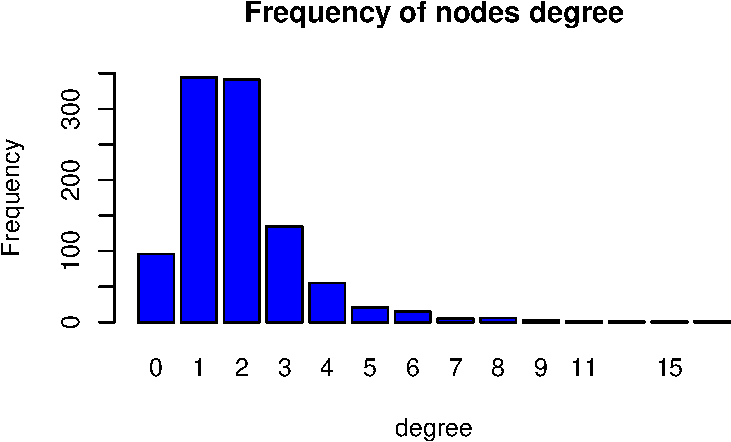
\includegraphics[width=1\textwidth,height=\textheight]{index_files/figure-pdf/unnamed-chunk-15-1.pdf}

}

\end{figure}

\hypertarget{mdag-global-core-for-eukaryotes}{%
\section{mDag Global core for
eukaryotes}\label{mdag-global-core-for-eukaryotes}}

Note that the mDAG core is empty as it does not contain any reactions.

\hypertarget{core-mdag}{%
\subsection{Core mDAG}\label{core-mdag}}

\begin{Shaded}
\begin{Highlighting}[]
\NormalTok{graph\_core\_mDAG}\OtherTok{=}\FunctionTok{read.graph}\NormalTok{(}
  \FunctionTok{paste0}\NormalTok{(path\_exp,}\StringTok{"Global/core/core\_mDAG.graphml"}\NormalTok{), }\AttributeTok{format =} \StringTok{"graphml"}\NormalTok{)}
\FunctionTok{summary}\NormalTok{(graph\_core\_mDAG)}
\end{Highlighting}
\end{Shaded}

\begin{verbatim}
IGRAPH f75f9ba D--- 0 0 -- 
+ attr: color (v/c), label (v/c), id (v/c)
\end{verbatim}

\begin{Shaded}
\begin{Highlighting}[]
\CommentTok{\# file missing}
\CommentTok{\#knitr::include\_graphics(paste0(path\_exp,"Global/core/core\_mDAG.pdf"))}
\end{Highlighting}
\end{Shaded}

The graph core mDAG have 0 vertex and 0, is an empty graph.

\hypertarget{core-reaction-graph-rc}{%
\subsection{Core reaction graph (RC)}\label{core-reaction-graph-rc}}

\begin{Shaded}
\begin{Highlighting}[]
\NormalTok{graph\_core\_RC}\OtherTok{=}\FunctionTok{read.graph}\NormalTok{(}
  \FunctionTok{paste0}\NormalTok{(path\_exp,}\StringTok{"Global/core/core\_RC.graphml"}\NormalTok{), }\AttributeTok{format =} \StringTok{"graphml"}\NormalTok{)}
\FunctionTok{summary}\NormalTok{(graph\_core\_mDAG)}
\end{Highlighting}
\end{Shaded}

\begin{verbatim}
IGRAPH f75f9ba D--- 0 0 -- 
+ attr: color (v/c), label (v/c), id (v/c)
\end{verbatim}

\begin{Shaded}
\begin{Highlighting}[]
\NormalTok{knitr}\SpecialCharTok{::}\FunctionTok{include\_graphics}\NormalTok{(}
  \FunctionTok{paste0}\NormalTok{(path\_exp,}\StringTok{"Global/core/core\_RC.pdf"}\NormalTok{))}
\end{Highlighting}
\end{Shaded}

\begin{figure}[H]

{\centering 
\includegraphics[width=1\textwidth,height=\textheight]{data/result_bb261b6e-95c6-3e39-b82b-b68eea80e30b/data/Global/core/core_RC.pdf}

}

\caption{Core mDAG is empty}

\end{figure}

The graph core reaction graph have 0 vertex and 0, is an empty graph.

\hypertarget{mdag-global-pan-for-eukaryotes}{%
\section{mDag Global pan for
eukaryotes}\label{mdag-global-pan-for-eukaryotes}}

\hypertarget{pan-mdag}{%
\subsection{Pan mDAG}\label{pan-mdag}}

\begin{Shaded}
\begin{Highlighting}[]
\NormalTok{graph\_pan\_mDAG}\OtherTok{=}\FunctionTok{read.graph}\NormalTok{(}
  \FunctionTok{paste0}\NormalTok{(path\_exp,}\StringTok{"TaxonomyLevels/Kingdom/Animals/pan/Animals\_pan\_mDAG.graphml"}\NormalTok{), }\AttributeTok{format =} \StringTok{"graphml"}\NormalTok{)}
\FunctionTok{summary}\NormalTok{(graph\_pan\_mDAG)}
\end{Highlighting}
\end{Shaded}

\begin{verbatim}
IGRAPH f78e74c D--- 1184 1261 -- 
+ attr: color (v/c), label (v/c), id (v/c), id (e/c)
\end{verbatim}

The graph pan mDAG have 1184 vertex and 1261.

\hypertarget{pan-reaction-graph-rc}{%
\subsection{Pan Reaction graph (RC)}\label{pan-reaction-graph-rc}}

\begin{Shaded}
\begin{Highlighting}[]
\NormalTok{graph\_pan\_RC}\OtherTok{=}\FunctionTok{read.graph}\NormalTok{(}
  \FunctionTok{paste0}\NormalTok{(path\_exp,}\StringTok{"TaxonomyLevels/Kingdom/Animals/pan/Animals\_pan\_RC.graphml"}\NormalTok{), }\AttributeTok{format =} \StringTok{"graphml"}\NormalTok{)}
\FunctionTok{summary}\NormalTok{(graph\_pan\_RC)}
\end{Highlighting}
\end{Shaded}

\begin{verbatim}
IGRAPH f79cd5d D--- 4556 5798 -- 
+ attr: color (v/c), label (v/c), id (v/c), id (e/c)
\end{verbatim}

The graph pan reaction graph have 4556 vertex and 5798.

\begin{Shaded}
\begin{Highlighting}[]
\NormalTok{compo}\OtherTok{=}\FunctionTok{components}\NormalTok{(graph\_mDAG,}\AttributeTok{mode =} \StringTok{"weak"}\NormalTok{)}
\FunctionTok{str}\NormalTok{(compo)}
\end{Highlighting}
\end{Shaded}

\begin{verbatim}
List of 3
 $ membership: num [1:1026] 1 1 1 1 1 1 1 1 1 1 ...
 $ csize     : num [1:167] 589 1 1 1 1 1 4 3 4 3 ...
 $ no        : int 167
\end{verbatim}

\begin{Shaded}
\begin{Highlighting}[]
\NormalTok{compo}\SpecialCharTok{$}\NormalTok{csize}
\end{Highlighting}
\end{Shaded}

\begin{verbatim}
  [1] 589   1   1   1   1   1   4   3   4   3   2   3   3   1   1   1   2   6
 [19]   3   1   3   6   1   1   1   1   1   3   1   6   2   1   1   1   2   1
 [37]   1  14   1  16   1   6   2   2   4   1   1   1   1   1   1   1   1   1
 [55]  13   1   1   1   1   2   6   5   5   2   2  10   1   1   1   2   2   1
 [73]   1   1  62   6   2   1   2   1   1   1   2   1   2  14   3   1   1   1
 [91]   1   1   1   1   1   1   3   6   1   3   1   3   2   1   1   1   2   2
[109]   3   1   1   2   5   1   1   2   3   2   1   1   2   3   4   1   1   2
[127]   1   1   2   1   1   1   1   1   3   1   2   2   1   6   1   1   1   2
[145]   1   1   1   1   1   2   7   1  15   3   1   1   1   1   2   1   3   1
[163]   1   1   1   1   2
\end{verbatim}

\begin{Shaded}
\begin{Highlighting}[]
\NormalTok{k}\OtherTok{=}\FunctionTok{which.max}\NormalTok{(compo}\SpecialCharTok{$}\NormalTok{csize}\SpecialCharTok{==}\FunctionTok{max}\NormalTok{(compo}\SpecialCharTok{$}\NormalTok{csize))}
\NormalTok{k}
\end{Highlighting}
\end{Shaded}

\begin{verbatim}
[1] 1
\end{verbatim}

\begin{Shaded}
\begin{Highlighting}[]
\FunctionTok{table}\NormalTok{(compo}\SpecialCharTok{$}\NormalTok{membership)}
\end{Highlighting}
\end{Shaded}

\begin{verbatim}

  1   2   3   4   5   6   7   8   9  10  11  12  13  14  15  16  17  18  19  20 
589   1   1   1   1   1   4   3   4   3   2   3   3   1   1   1   2   6   3   1 
 21  22  23  24  25  26  27  28  29  30  31  32  33  34  35  36  37  38  39  40 
  3   6   1   1   1   1   1   3   1   6   2   1   1   1   2   1   1  14   1  16 
 41  42  43  44  45  46  47  48  49  50  51  52  53  54  55  56  57  58  59  60 
  1   6   2   2   4   1   1   1   1   1   1   1   1   1  13   1   1   1   1   2 
 61  62  63  64  65  66  67  68  69  70  71  72  73  74  75  76  77  78  79  80 
  6   5   5   2   2  10   1   1   1   2   2   1   1   1  62   6   2   1   2   1 
 81  82  83  84  85  86  87  88  89  90  91  92  93  94  95  96  97  98  99 100 
  1   1   2   1   2  14   3   1   1   1   1   1   1   1   1   1   3   6   1   3 
101 102 103 104 105 106 107 108 109 110 111 112 113 114 115 116 117 118 119 120 
  1   3   2   1   1   1   2   2   3   1   1   2   5   1   1   2   3   2   1   1 
121 122 123 124 125 126 127 128 129 130 131 132 133 134 135 136 137 138 139 140 
  2   3   4   1   1   2   1   1   2   1   1   1   1   1   3   1   2   2   1   6 
141 142 143 144 145 146 147 148 149 150 151 152 153 154 155 156 157 158 159 160 
  1   1   1   2   1   1   1   1   1   2   7   1  15   3   1   1   1   1   2   1 
161 162 163 164 165 166 167 
  3   1   1   1   1   1   2 
\end{verbatim}

\begin{Shaded}
\begin{Highlighting}[]
\NormalTok{vertex}\OtherTok{=}\FunctionTok{which}\NormalTok{(compo}\SpecialCharTok{$}\NormalTok{membership}\SpecialCharTok{==}\NormalTok{k)}
\FunctionTok{length}\NormalTok{(vertex)}
\end{Highlighting}
\end{Shaded}

\begin{verbatim}
[1] 589
\end{verbatim}

\begin{Shaded}
\begin{Highlighting}[]
\NormalTok{Big\_Component}\OtherTok{=}\FunctionTok{induced\_subgraph}\NormalTok{(graph\_mDAG, }\AttributeTok{vids=}\NormalTok{vertex)}
\NormalTok{igraph}\SpecialCharTok{::}\FunctionTok{vcount}\NormalTok{(Big\_Component)}
\end{Highlighting}
\end{Shaded}

\begin{verbatim}
[1] 589
\end{verbatim}

\begin{Shaded}
\begin{Highlighting}[]
\NormalTok{igraph}\SpecialCharTok{::}\FunctionTok{ecount}\NormalTok{(Big\_Component)}
\end{Highlighting}
\end{Shaded}

\begin{verbatim}
[1] 774
\end{verbatim}

The curated plot of the bigger component of hsa mDAG

\begin{Shaded}
\begin{Highlighting}[]
\CommentTok{\#knitr::include\_graphics(paste0(path\_exp,}
\CommentTok{\#                              "Individuals/hsa/hsa\_mDAG\_biggerDAG.pdf"))}
\end{Highlighting}
\end{Shaded}

\bookmarksetup{startatroot}

\hypertarget{similarities-and-metadata-for-an-experiment}{%
\chapter{Similarities and metadata for an
experiment}\label{similarities-and-metadata-for-an-experiment}}

We will first load the metadata and adapt them to the structure of the
similarities to facilitate the creation of the graphs and statistics.

Remenber de path of the experiment:

\begin{Shaded}
\begin{Highlighting}[]
\NormalTok{path\_exp}
\end{Highlighting}
\end{Shaded}

\begin{verbatim}
[1] "data/result_bb261b6e-95c6-3e39-b82b-b68eea80e30b/data/"
\end{verbatim}

\hypertarget{load-meta-data-from-eukariotes-experimet}{%
\section{Load meta data from eukariotes
experimet}\label{load-meta-data-from-eukariotes-experimet}}

Meta data mDa\_Id and taxonomy sort by Kingdom,Filum,Class,mDAG\_Id

\begin{Shaded}
\begin{Highlighting}[]
\NormalTok{path\_exp}
\end{Highlighting}
\end{Shaded}

\begin{verbatim}
[1] "data/result_bb261b6e-95c6-3e39-b82b-b68eea80e30b/data/"
\end{verbatim}

\begin{Shaded}
\begin{Highlighting}[]
\NormalTok{Results}\OtherTok{=}\FunctionTok{read\_csv}\NormalTok{(}\FunctionTok{paste0}\NormalTok{(path\_exp,}\StringTok{"Results.csv"}\NormalTok{))}
\FunctionTok{names}\NormalTok{(Results)[}\FunctionTok{c}\NormalTok{(}\DecValTok{1}\NormalTok{,}\DecValTok{3}\NormalTok{,}\DecValTok{4}\NormalTok{)]}\OtherTok{=}\FunctionTok{c}\NormalTok{(}\StringTok{"Organism"}\NormalTok{,}\StringTok{"mDAG\_Id"}\NormalTok{,}\StringTok{"Full\_Name"}\NormalTok{)}
\NormalTok{taxo}\OtherTok{=}\NormalTok{Results }\SpecialCharTok{\%\textgreater{}\%} \FunctionTok{select}\NormalTok{(Organism}\SpecialCharTok{:}\NormalTok{Full\_Name)}
\NormalTok{taxo}\OtherTok{=}\NormalTok{taxo }\SpecialCharTok{\%\textgreater{}\%} \FunctionTok{separate}\NormalTok{(Categories,}\AttributeTok{into=}\FunctionTok{c}\NormalTok{(}\StringTok{"Kingdom"}\NormalTok{,}\StringTok{"Phylum"}\NormalTok{,}\StringTok{"Class"}\NormalTok{))}
\NormalTok{index}\OtherTok{=}\FunctionTok{which}\NormalTok{(}\FunctionTok{is.na}\NormalTok{(taxo}\SpecialCharTok{$}\NormalTok{Class))}
\NormalTok{taxo}\SpecialCharTok{$}\NormalTok{Class[index]}\OtherTok{=}\FunctionTok{paste}\NormalTok{(taxo}\SpecialCharTok{$}\NormalTok{Phylum[index])}
\NormalTok{meta\_taxo}\OtherTok{=}\NormalTok{taxo}
\NormalTok{aux}\OtherTok{=}\FunctionTok{table}\NormalTok{(meta\_taxo}\SpecialCharTok{$}\NormalTok{Phylum)}
\NormalTok{Freq\_Phylum}\OtherTok{=}\FunctionTok{tibble}\NormalTok{(}\AttributeTok{Phylum=}\FunctionTok{names}\NormalTok{(aux),}\AttributeTok{Freq\_Phylum=}\NormalTok{aux)}
\FunctionTok{names}\NormalTok{(Freq\_Phylum)}\OtherTok{=}\FunctionTok{c}\NormalTok{(}\StringTok{"Phylum"}\NormalTok{,}\StringTok{"Freq\_Phylum"}\NormalTok{)}
\NormalTok{aux}\OtherTok{=}\FunctionTok{table}\NormalTok{(meta\_taxo}\SpecialCharTok{$}\NormalTok{Class)}
\NormalTok{Freq\_Class}\OtherTok{=}\FunctionTok{tibble}\NormalTok{(}\AttributeTok{Class=}\FunctionTok{names}\NormalTok{(aux),}\AttributeTok{Freq\_Class=}\NormalTok{aux)}
\FunctionTok{names}\NormalTok{(Freq\_Class)}\OtherTok{=}\FunctionTok{c}\NormalTok{(}\StringTok{"Class"}\NormalTok{,}\StringTok{"Freq\_Class"}\NormalTok{)}


\NormalTok{meta\_taxo }\OtherTok{=}\NormalTok{ meta\_taxo }\SpecialCharTok{\%\textgreater{}\%} \FunctionTok{left\_join}\NormalTok{(Freq\_Phylum) }\SpecialCharTok{\%\textgreater{}\%} \FunctionTok{left\_join}\NormalTok{(Freq\_Class)}
\NormalTok{meta\_taxo }\OtherTok{=}\NormalTok{ meta\_taxo }\SpecialCharTok{\%\textgreater{}\%}  \FunctionTok{arrange}\NormalTok{(Kingdom,}\FunctionTok{desc}\NormalTok{(Freq\_Phylum),Phylum,}\FunctionTok{desc}\NormalTok{(Freq\_Class),Class)}
\FunctionTok{head}\NormalTok{(meta\_taxo)}
\end{Highlighting}
\end{Shaded}

\begin{verbatim}
# A tibble: 6 x 8
  Organism Kingdom Phylum      Class   mDAG_Id Full_Name  Freq_Phylum Freq_Class
  <chr>    <chr>   <chr>       <chr>   <chr>   <chr>      <table[1d]> <table[1d>
1 aamp     Animals Vertebrates Mammals 0313    Arvicola ~ 331         139       
2 afz      Animals Vertebrates Mammals 0143    Antechinu~ 331         139       
3 ajm      Animals Vertebrates Mammals 0221    Artibeus ~ 331         139       
4 aju      Animals Vertebrates Mammals 0224    Acinonyx ~ 331         139       
5 aml      Animals Vertebrates Mammals 0279    Ailuropod~ 331         139       
6 anu      Animals Vertebrates Mammals 0310    Arvicanth~ 331         139       
\end{verbatim}

\begin{Shaded}
\begin{Highlighting}[]
\FunctionTok{table}\NormalTok{(meta\_taxo}\SpecialCharTok{$}\NormalTok{Kingdom) }\SpecialCharTok{\%\textgreater{}\%}\NormalTok{ kable }\SpecialCharTok{\%\textgreater{}\%}
  \FunctionTok{kable\_styling}\NormalTok{(}\StringTok{"striped"}\NormalTok{, }\AttributeTok{full\_width =}\NormalTok{ F,}\AttributeTok{position=}\StringTok{"left"}\NormalTok{)}\SpecialCharTok{\%\textgreater{}\%} 
 \FunctionTok{scroll\_box}\NormalTok{(}\AttributeTok{width =} \StringTok{"400px"}\NormalTok{, }\AttributeTok{height =} \StringTok{"200px"}\NormalTok{)}
\end{Highlighting}
\end{Shaded}

\begin{tabular}{l|r}
\hline
Var1 & Freq\\
\hline
Animals & 535\\
\hline
Fungi & 154\\
\hline
Plants & 139\\
\hline
Protists & 56\\
\hline
\end{tabular}

\begin{Shaded}
\begin{Highlighting}[]
\FunctionTok{table}\NormalTok{(meta\_taxo}\SpecialCharTok{$}\NormalTok{Phylum,meta\_taxo}\SpecialCharTok{$}\NormalTok{Kingdom) }\SpecialCharTok{\%\textgreater{}\%}\NormalTok{ kable }\SpecialCharTok{\%\textgreater{}\%}
  \FunctionTok{kable\_styling}\NormalTok{(}\StringTok{"striped"}\NormalTok{, }\AttributeTok{full\_width =}\NormalTok{ F,}\AttributeTok{position=}\StringTok{"left"}\NormalTok{)}\SpecialCharTok{\%\textgreater{}\%} 
 \FunctionTok{scroll\_box}\NormalTok{(}\AttributeTok{width =} \StringTok{"500px"}\NormalTok{, }\AttributeTok{height =} \StringTok{"500px"}\NormalTok{)}
\end{Highlighting}
\end{Shaded}

\begin{tabular}{l|r|r|r|r}
\hline
  & Animals & Fungi & Plants & Protists\\
\hline
Alveolates & 0 & 0 & 0 & 25\\
\hline
Amoebozoa & 0 & 0 & 0 & 7\\
\hline
Annelids & 1 & 0 & 0 & 0\\
\hline
Arthropods & 158 & 0 & 0 & 0\\
\hline
Ascomycetes & 0 & 113 & 0 & 0\\
\hline
Basal & 0 & 0 & 2 & 0\\
\hline
Basidiomycetes & 0 & 36 & 0 & 0\\
\hline
Brachiopodas & 1 & 0 & 0 & 0\\
\hline
Cephalochordates & 2 & 0 & 0 & 0\\
\hline
Choanoflagellates & 0 & 0 & 0 & 2\\
\hline
Cnidarians & 10 & 0 & 0 & 0\\
\hline
Cryptomonads & 0 & 0 & 0 & 1\\
\hline
Echinoderms & 3 & 0 & 0 & 0\\
\hline
Eudicots & 0 & 0 & 98 & 0\\
\hline
Euglenozoa & 0 & 0 & 0 & 9\\
\hline
Ferns & 0 & 0 & 1 & 0\\
\hline
Flatworms & 4 & 0 & 0 & 0\\
\hline
Green & 0 & 0 & 11 & 0\\
\hline
Haptophyta & 0 & 0 & 0 & 1\\
\hline
Hemichordates & 1 & 0 & 0 & 0\\
\hline
Heterolobosea & 0 & 0 & 0 & 1\\
\hline
Metamonada & 0 & 0 & 0 & 2\\
\hline
Microsporidians & 0 & 5 & 0 & 0\\
\hline
Mollusks & 14 & 0 & 0 & 0\\
\hline
Monocots & 0 & 0 & 23 & 0\\
\hline
Mosses & 0 & 0 & 1 & 0\\
\hline
Nematodes & 6 & 0 & 0 & 0\\
\hline
Placozoans & 1 & 0 & 0 & 0\\
\hline
Poriferans & 1 & 0 & 0 & 0\\
\hline
Red & 0 & 0 & 3 & 0\\
\hline
Stramenopiles & 0 & 0 & 0 & 8\\
\hline
Tunicates & 2 & 0 & 0 & 0\\
\hline
Vertebrates & 331 & 0 & 0 & 0\\
\hline
\end{tabular}

\hypertarget{similarities-msamunkres-methods}{%
\section{Similarities MSA,Munkres
methods}\label{similarities-msamunkres-methods}}

In this section we will show the similarities between mDAG's using
different methods.

The experiment data set consists of 884 eurkaryotes from the animal,
plant, fungus, and protist kingdoms.

\begin{tabular}{l|r}
\hline
Kingdom & Abs. Freq.\\
\hline
Animals & 535\\
\hline
Fungi & 154\\
\hline
Plants & 139\\
\hline
Protists & 56\\
\hline
\end{tabular}

\begin{Shaded}
\begin{Highlighting}[]
\NormalTok{list\_Sim}\OtherTok{=}\FunctionTok{dir}\NormalTok{(path\_exp,}\AttributeTok{pattern=}\StringTok{"\^{}Similarities"}\NormalTok{)}
\NormalTok{list\_Sim}
\end{Highlighting}
\end{Shaded}

\begin{verbatim}
[1] "Similarities_MBB_MSAMethod.csv"      "Similarities_MBB_MunkresMethod.csv" 
[3] "Similarities_mDAG_MSAMethod.csv"     "Similarities_mDAG_MunkresMethod.csv"
\end{verbatim}

Load MDAG similarities

\begin{Shaded}
\begin{Highlighting}[]
\NormalTok{Sim\_MSA\_mDAG}\OtherTok{=}\FunctionTok{read\_csv}\NormalTok{(}\FunctionTok{paste0}\NormalTok{(path\_exp,}
                             \StringTok{"Similarities\_mDAG\_MSAMethod.csv"}\NormalTok{))}
\NormalTok{Sim\_MSA\_mDAG}\OtherTok{=}\FunctionTok{as.matrix}\NormalTok{(Sim\_MSA\_mDAG[,}\SpecialCharTok{{-}}\DecValTok{1}\NormalTok{])}
\FunctionTok{rownames}\NormalTok{(Sim\_MSA\_mDAG)}\OtherTok{=}\FunctionTok{colnames}\NormalTok{(Sim\_MSA\_mDAG)}
\NormalTok{Sim\_MSA\_mDAG}\OtherTok{=}\NormalTok{Sim\_MSA\_mDAG[meta\_taxo}\SpecialCharTok{$}\NormalTok{mDAG\_Id,meta\_taxo}\SpecialCharTok{$}\NormalTok{mDAG\_Id]}
\end{Highlighting}
\end{Shaded}

\begin{Shaded}
\begin{Highlighting}[]
\NormalTok{Sim\_Mun\_mDAG}\OtherTok{=}\FunctionTok{read\_csv}\NormalTok{(}\FunctionTok{paste0}\NormalTok{(path\_exp,}
\StringTok{"Similarities\_mDAG\_MunkresMethod.csv"}\NormalTok{))}
\NormalTok{Sim\_Mun\_mDAG}\OtherTok{=}\FunctionTok{as.matrix}\NormalTok{(Sim\_Mun\_mDAG[,}\SpecialCharTok{{-}}\DecValTok{1}\NormalTok{])}
\FunctionTok{rownames}\NormalTok{(Sim\_Mun\_mDAG)}\OtherTok{=}\FunctionTok{colnames}\NormalTok{(Sim\_Mun\_mDAG)}
\NormalTok{Sim\_Mun\_mDAG}\OtherTok{=}\NormalTok{Sim\_Mun\_mDAG[meta\_taxo}\SpecialCharTok{$}\NormalTok{mDAG\_Id,meta\_taxo}\SpecialCharTok{$}\NormalTok{mDAG\_Id]}
\end{Highlighting}
\end{Shaded}

\hypertarget{heatmaps}{%
\section{Heatmaps}\label{heatmaps}}

\hypertarget{heatmap-similarity-msa-and-munkres-method}{%
\subsection{Heatmap Similarity MSA and Munkres
method}\label{heatmap-similarity-msa-and-munkres-method}}

\begin{Shaded}
\begin{Highlighting}[]
\NormalTok{dff}\OtherTok{\textless{}{-}}\NormalTok{meta\_taxo }\SpecialCharTok{\%\textgreater{}\%} \FunctionTok{select}\NormalTok{(Kingdom)  }\SpecialCharTok{\%\textgreater{}\%} \FunctionTok{as.data.frame}\NormalTok{()}
\NormalTok{colorsK }\OtherTok{\textless{}{-}} \FunctionTok{list}\NormalTok{(}\AttributeTok{Kingdom=} \FunctionTok{c}\NormalTok{(}\StringTok{"Animals"}\OtherTok{=}\StringTok{"red"}\NormalTok{,}
                           \StringTok{"Plants"}\OtherTok{=}\StringTok{"green"}\NormalTok{,}
                           \StringTok{"Fungi"}\OtherTok{=}\StringTok{"yellow"}\NormalTok{,}
                           \StringTok{"Protists"}\OtherTok{=}\StringTok{"black"}\NormalTok{))}
\NormalTok{annotationK }\OtherTok{\textless{}{-}} \FunctionTok{HeatmapAnnotation}\NormalTok{(}\AttributeTok{df=}\NormalTok{dff, }\AttributeTok{col =}\NormalTok{ colorsK,}\AttributeTok{show\_legend =} \ConstantTok{TRUE}\NormalTok{)}

\NormalTok{MSA\_heat\_1 }\OtherTok{\textless{}{-}} \FunctionTok{Heatmap}\NormalTok{(}\AttributeTok{matrix =}\NormalTok{ Sim\_MSA\_mDAG, }
                      \AttributeTok{column\_title=}
                        \StringTok{"m{-}DAGs MSA{-}similarity Eukaryotes by Kingdoms"}\NormalTok{,}
                      \AttributeTok{heatmap\_legend\_param=}\FunctionTok{list}\NormalTok{(}
                        \AttributeTok{title=}\StringTok{"Similarity"}\NormalTok{,}
                        \AttributeTok{at =} \FunctionTok{seq}\NormalTok{(}\DecValTok{0}\NormalTok{,}\DecValTok{1}\NormalTok{,}\AttributeTok{by=}\FloatTok{0.1}\NormalTok{)),}
                      \AttributeTok{col=}\FunctionTok{rev}\NormalTok{(}\FunctionTok{viridis}\NormalTok{(}\DecValTok{256}\NormalTok{)),}
                      \AttributeTok{cluster\_rows =} \ConstantTok{FALSE}\NormalTok{,}
                      \AttributeTok{cluster\_columns =} \ConstantTok{FALSE}\NormalTok{,}
                      \AttributeTok{top\_annotation =}\NormalTok{ annotationK,}
                      \AttributeTok{show\_column\_names =} \ConstantTok{FALSE}\NormalTok{, }
                      \AttributeTok{show\_row\_names =} \ConstantTok{FALSE}\NormalTok{,}
                      \AttributeTok{left\_annotation =}
                        \FunctionTok{rowAnnotation}\NormalTok{(}\AttributeTok{df =}\NormalTok{ dff,}
                                      \AttributeTok{col =}\NormalTok{ colorsK,}
                                    \AttributeTok{show\_annotation\_name=}\ConstantTok{FALSE}\NormalTok{,}
                                    \AttributeTok{show\_legend=}\ConstantTok{FALSE}
\NormalTok{                                      ))}







\NormalTok{Mun\_heat\_1}\OtherTok{\textless{}{-}} \FunctionTok{Heatmap}\NormalTok{(}\AttributeTok{matrix =}\NormalTok{ Sim\_Mun\_mDAG, }
             \AttributeTok{column\_title=}\StringTok{"mDAGs Munkres{-}similarity  Eukaryotes by Kingdoms"}\NormalTok{,}
            \AttributeTok{name =} \StringTok{"Munkres Similarity"}\NormalTok{,}
            \AttributeTok{heatmap\_legend\_param=}\FunctionTok{list}\NormalTok{(}
                        \AttributeTok{title=}\StringTok{"Similarity"}\NormalTok{,}
                        \AttributeTok{at =} \FunctionTok{seq}\NormalTok{(}\DecValTok{0}\NormalTok{,}\DecValTok{1}\NormalTok{,}\AttributeTok{by=}\FloatTok{0.1}\NormalTok{)),}
                      \AttributeTok{col=}\FunctionTok{rev}\NormalTok{(}\FunctionTok{viridis}\NormalTok{(}\DecValTok{256}\NormalTok{)),}
                      \AttributeTok{cluster\_rows =} \ConstantTok{FALSE}\NormalTok{,}
                      \AttributeTok{cluster\_columns =} \ConstantTok{FALSE}\NormalTok{,}
                      \AttributeTok{top\_annotation =}\NormalTok{ annotationK,}
                      \AttributeTok{show\_column\_names =} \ConstantTok{FALSE}\NormalTok{, }
                      \AttributeTok{show\_row\_names =} \ConstantTok{FALSE}\NormalTok{,}
                      \AttributeTok{left\_annotation =}
                        \FunctionTok{rowAnnotation}\NormalTok{(}\AttributeTok{df =}\NormalTok{ dff,}
                                      \AttributeTok{col =}\NormalTok{ colorsK,}
                                    \AttributeTok{show\_annotation\_name=}\ConstantTok{FALSE}\NormalTok{,}
                                    \AttributeTok{show\_legend=}\ConstantTok{FALSE}
\NormalTok{                                      ))}
\end{Highlighting}
\end{Shaded}

\begin{Shaded}
\begin{Highlighting}[]
\NormalTok{meta\_animals}\OtherTok{=}\NormalTok{ meta\_taxo }\SpecialCharTok{\%\textgreater{}\%} \FunctionTok{filter}\NormalTok{(Kingdom}\SpecialCharTok{==}\StringTok{"Animals"}\NormalTok{)}
\NormalTok{dff}\OtherTok{\textless{}{-}}\NormalTok{meta\_taxo }\SpecialCharTok{\%\textgreater{}\%} \FunctionTok{filter}\NormalTok{(Kingdom}\SpecialCharTok{==}\StringTok{"Animals"}\NormalTok{) }\SpecialCharTok{\%\textgreater{}\%} \FunctionTok{select}\NormalTok{(Phylum,Freq\_Phylum) }\SpecialCharTok{\%\textgreater{}\%}   \FunctionTok{as.data.frame}\NormalTok{() }\SpecialCharTok{\%\textgreater{}\%} \FunctionTok{select}\NormalTok{(Phylum)}
\NormalTok{namesP}\OtherTok{=}\NormalTok{dff }\SpecialCharTok{\%\textgreater{}\%} \FunctionTok{distinct}\NormalTok{( Phylum, }\AttributeTok{.keep\_all =} \ConstantTok{TRUE}\NormalTok{) }
\NormalTok{namesP}\OtherTok{=}\NormalTok{namesP}\SpecialCharTok{$}\NormalTok{Phylum}
\NormalTok{dff}\SpecialCharTok{$}\NormalTok{Phylum}\OtherTok{=}\FunctionTok{ordered}\NormalTok{(dff}\SpecialCharTok{$}\NormalTok{Phylum,}\AttributeTok{labels=}\NormalTok{namesP)}
\NormalTok{col}\OtherTok{=}\FunctionTok{rainbow}\NormalTok{(}\FunctionTok{length}\NormalTok{(namesP))}
\NormalTok{colorsP}\OtherTok{=}\FunctionTok{list}\NormalTok{(}\AttributeTok{Phylum=}\NormalTok{col)}
\FunctionTok{names}\NormalTok{(colorsP}\SpecialCharTok{$}\NormalTok{Phylum)}\OtherTok{=}\NormalTok{namesP}
\NormalTok{annotation\_H2 }\OtherTok{\textless{}{-}} \FunctionTok{HeatmapAnnotation}\NormalTok{(}\AttributeTok{df=}\NormalTok{dff, }\AttributeTok{col =}\NormalTok{ colorsP)}
\NormalTok{MSA\_heat\_2 }\OtherTok{\textless{}{-}} \FunctionTok{Heatmap}\NormalTok{(}\AttributeTok{matrix =}
\NormalTok{                        Sim\_MSA\_mDAG[}\DecValTok{1}\SpecialCharTok{:}\FunctionTok{nrow}\NormalTok{(dff),}\DecValTok{1}\SpecialCharTok{:}\FunctionTok{nrow}\NormalTok{(dff)],}
                      \AttributeTok{column\_title=}\StringTok{"mDAGs MSA{-}similarity  Animals by Phyla"}\NormalTok{,}
                      \AttributeTok{col=}\FunctionTok{rev}\NormalTok{(}\FunctionTok{viridis}\NormalTok{(}\DecValTok{256}\NormalTok{)),}
                      \AttributeTok{cluster\_rows =} \ConstantTok{FALSE}\NormalTok{,}
                      \AttributeTok{show\_heatmap\_legend=}\ConstantTok{FALSE}\NormalTok{, }
                      \AttributeTok{cluster\_columns =} \ConstantTok{FALSE}\NormalTok{,}
                      \AttributeTok{top\_annotation =}\NormalTok{ annotation\_H2,}
                      \AttributeTok{show\_column\_names =} \ConstantTok{FALSE}\NormalTok{, }
                      \AttributeTok{show\_row\_names =} \ConstantTok{FALSE}\NormalTok{,}
                      \AttributeTok{left\_annotation =} 
                        \FunctionTok{rowAnnotation}\NormalTok{(}\AttributeTok{df =}\NormalTok{ dff,}
                                      \AttributeTok{col =}\NormalTok{ colorsP,}
                                      \AttributeTok{show\_annotation\_name=}\ConstantTok{FALSE}\NormalTok{,}
                                      \AttributeTok{show\_legend =}\ConstantTok{FALSE}
\NormalTok{                                      ))}



\NormalTok{Mun\_heat\_2 }\OtherTok{\textless{}{-}} \FunctionTok{Heatmap}\NormalTok{(}\AttributeTok{matrix =}\NormalTok{ Sim\_Mun\_mDAG[}\DecValTok{1}\SpecialCharTok{:}\FunctionTok{nrow}\NormalTok{(dff),}\DecValTok{1}\SpecialCharTok{:}\FunctionTok{nrow}\NormalTok{(dff)], }
              \AttributeTok{column\_title=}\StringTok{"mDAGs Munkres{-}similarity  Animals by Phyla"}\NormalTok{,}
        \AttributeTok{col=}\FunctionTok{rev}\NormalTok{(}\FunctionTok{viridis}\NormalTok{(}\DecValTok{256}\NormalTok{)),}
    \AttributeTok{show\_heatmap\_legend=}\ConstantTok{FALSE}\NormalTok{, }
        \AttributeTok{cluster\_rows =} \ConstantTok{FALSE}\NormalTok{,}
        \AttributeTok{cluster\_columns =} \ConstantTok{FALSE}\NormalTok{,}
        \AttributeTok{top\_annotation =}\NormalTok{ annotation\_H2,}
        \AttributeTok{show\_column\_names =} \ConstantTok{FALSE}\NormalTok{, }
        \AttributeTok{show\_row\_names =} \ConstantTok{FALSE}\NormalTok{,}
        \AttributeTok{left\_annotation =} \FunctionTok{rowAnnotation}\NormalTok{(}\AttributeTok{df =}\NormalTok{ dff,}
                                        \AttributeTok{col =}\NormalTok{ colorsP,}
                                    \AttributeTok{show\_annotation\_name=}\ConstantTok{FALSE}\NormalTok{,}
                                        \AttributeTok{show\_legend =}\ConstantTok{FALSE}
\NormalTok{                                        ))}
\end{Highlighting}
\end{Shaded}

\begin{Shaded}
\begin{Highlighting}[]
\NormalTok{MSA\_heat\_1}
\end{Highlighting}
\end{Shaded}

\begin{figure}[H]

{\centering 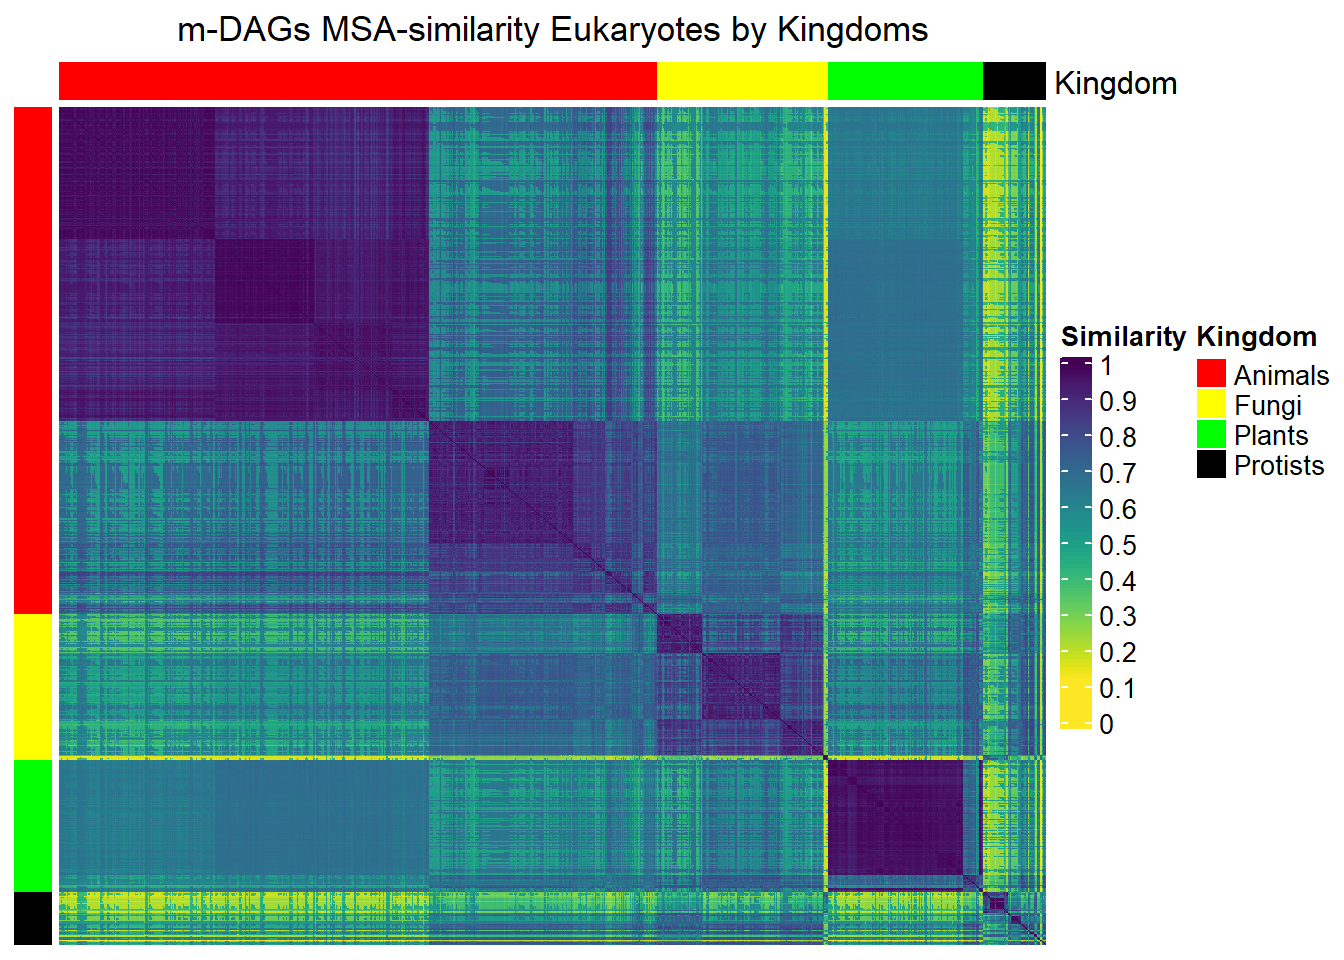
\includegraphics[width=1\textwidth,height=\textheight]{index_files/figure-pdf/heatmaps-1.pdf}

}

\end{figure}

\begin{Shaded}
\begin{Highlighting}[]
\NormalTok{MSA\_heat\_2}
\end{Highlighting}
\end{Shaded}

\begin{figure}[H]

{\centering 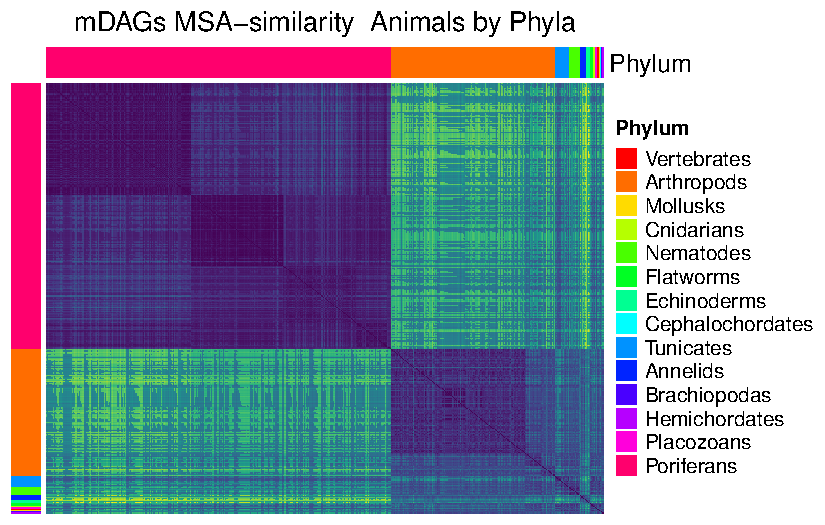
\includegraphics[width=1\textwidth,height=\textheight]{index_files/figure-pdf/heatmaps-2.pdf}

}

\end{figure}

\begin{Shaded}
\begin{Highlighting}[]
\NormalTok{Mun\_heat\_1}
\end{Highlighting}
\end{Shaded}

\begin{figure}[H]

{\centering 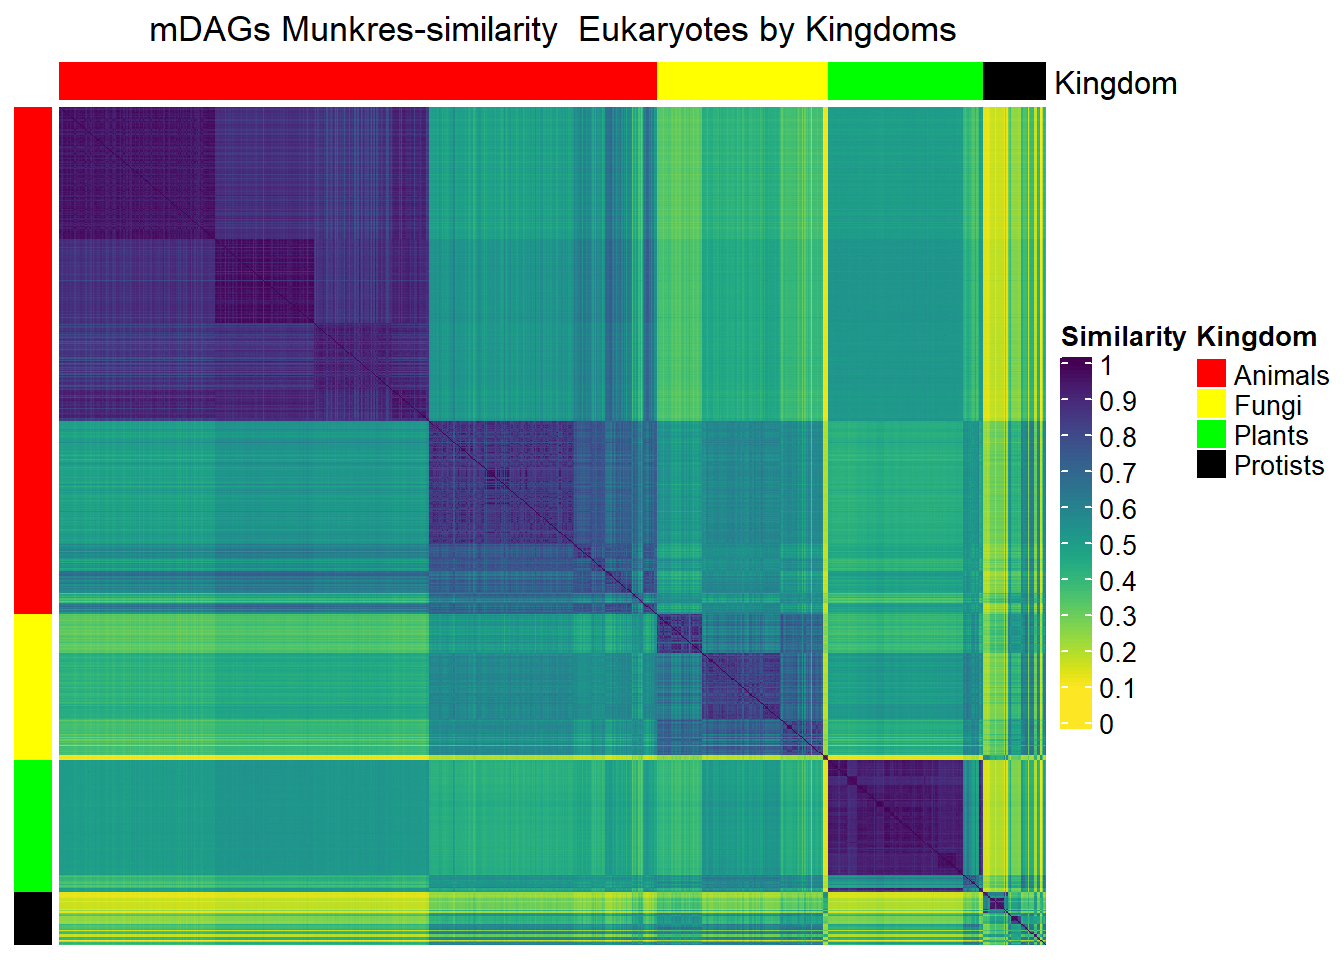
\includegraphics[width=1\textwidth,height=\textheight]{index_files/figure-pdf/heatmaps-3.pdf}

}

\end{figure}

\begin{Shaded}
\begin{Highlighting}[]
\NormalTok{Mun\_heat\_2}
\end{Highlighting}
\end{Shaded}

\begin{figure}[H]

{\centering 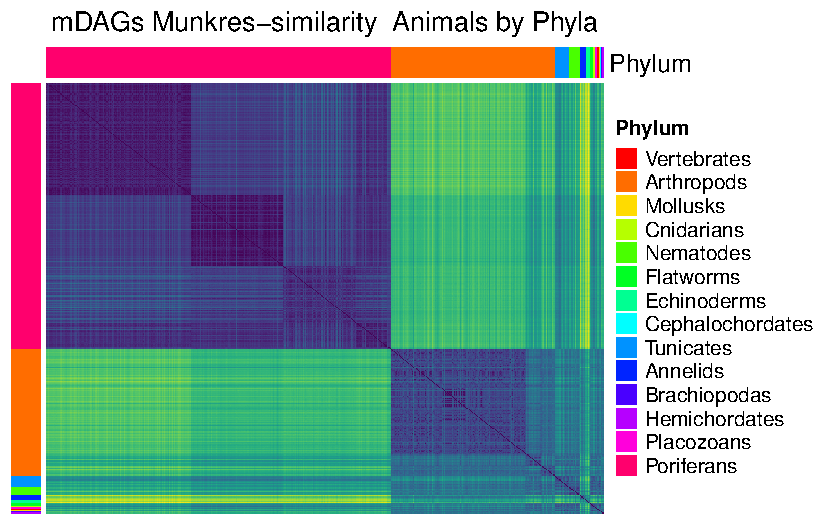
\includegraphics[width=1\textwidth,height=\textheight]{index_files/figure-pdf/heatmaps-4.pdf}

}

\end{figure}

\hypertarget{mds-multidimensional-scaling-msa}{%
\section{MDS (Multidimensional Scaling)
MSA}\label{mds-multidimensional-scaling-msa}}

\begin{Shaded}
\begin{Highlighting}[]
\DocumentationTok{\#\# Metric multidimensional scaling (mMDS)}
\NormalTok{mds7 }\OtherTok{\textless{}{-}} \FunctionTok{cmdscale}\NormalTok{(}\FunctionTok{sqrt}\NormalTok{(}\DecValTok{1}\SpecialCharTok{{-}}\NormalTok{Sim\_MSA\_mDAG}\SpecialCharTok{\^{}}\DecValTok{2}\NormalTok{),}\AttributeTok{k=}\DecValTok{7}\NormalTok{,}\AttributeTok{eig=}\ConstantTok{TRUE}\NormalTok{)}
\CommentTok{\#pairs(mds7$points[,1:4])}
\NormalTok{mds7}\SpecialCharTok{$}\NormalTok{GOF}
\end{Highlighting}
\end{Shaded}

\begin{verbatim}
[1] 0.4406568 0.5541042
\end{verbatim}

\begin{Shaded}
\begin{Highlighting}[]
\NormalTok{mds }\OtherTok{\textless{}{-}}\NormalTok{ mds7}\SpecialCharTok{$}\NormalTok{points }\SpecialCharTok{\%\textgreater{}\%}  \FunctionTok{as\_tibble}\NormalTok{()}
\FunctionTok{colnames}\NormalTok{(mds) }\OtherTok{\textless{}{-}}\FunctionTok{paste0}\NormalTok{(}\StringTok{"Dim."}\NormalTok{,}\DecValTok{1}\SpecialCharTok{:}\FunctionTok{dim}\NormalTok{(mds7}\SpecialCharTok{$}\NormalTok{points)[}\DecValTok{2}\NormalTok{])}


\NormalTok{cooordinates}\OtherTok{=}\FunctionTok{as\_tibble}\NormalTok{(mds7}\SpecialCharTok{$}\NormalTok{points)}
\FunctionTok{colnames}\NormalTok{(cooordinates)}\OtherTok{=}\FunctionTok{paste}\NormalTok{(}\StringTok{"Component"}\NormalTok{,}\DecValTok{1}\SpecialCharTok{:}\DecValTok{7}\NormalTok{)}
\FunctionTok{ggpairs}\NormalTok{(cooordinates,}\AttributeTok{columns=}\DecValTok{1}\SpecialCharTok{:}\DecValTok{4}\NormalTok{,}\FunctionTok{aes}\NormalTok{(}\AttributeTok{color=}\NormalTok{meta\_taxo}\SpecialCharTok{$}\NormalTok{Kingdom,}\AttributeTok{alpha=}\FloatTok{0.5}\NormalTok{,}\AttributeTok{title=}\StringTok{"MDS 4 dimensions projection"}\NormalTok{,}\AttributeTok{legend=}\DecValTok{1}\NormalTok{),}\AttributeTok{upper=}\FunctionTok{list}\NormalTok{(}\AttributeTok{continuous=}\StringTok{"points"}\NormalTok{)) }\SpecialCharTok{+}\FunctionTok{scale\_fill\_manual}\NormalTok{(}\AttributeTok{values =}\NormalTok{ colorsK}\SpecialCharTok{$}\NormalTok{Kingdom)}\SpecialCharTok{+} \FunctionTok{theme}\NormalTok{(}\AttributeTok{legend.position =} \StringTok{"left"}\NormalTok{)}
\end{Highlighting}
\end{Shaded}

\begin{figure}[H]

{\centering 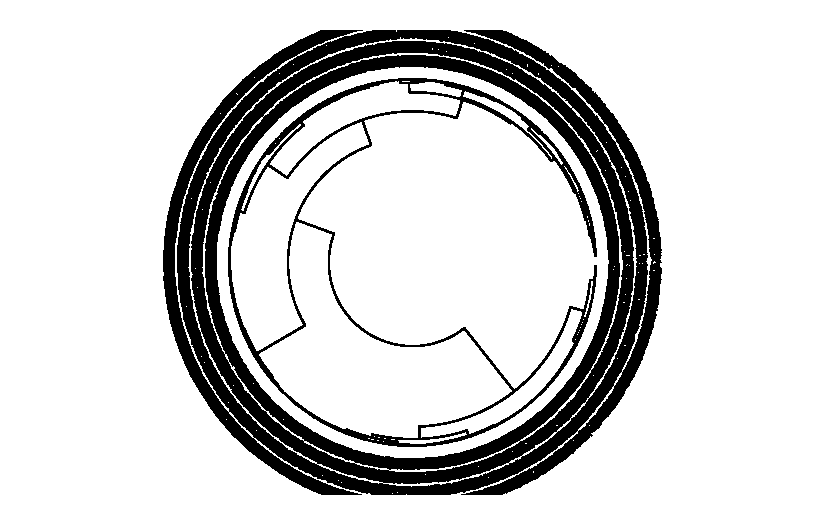
\includegraphics[width=1\textwidth,height=\textheight]{index_files/figure-pdf/unnamed-chunk-34-1.pdf}

}

\end{figure}

\begin{Shaded}
\begin{Highlighting}[]
\NormalTok{mds }\OtherTok{\textless{}{-}}\NormalTok{ mds }\SpecialCharTok{\%\textgreater{}\%}
  \FunctionTok{mutate}\NormalTok{(}\AttributeTok{groups =}\FunctionTok{as.factor}\NormalTok{(meta\_taxo}\SpecialCharTok{$}\NormalTok{Kingdom))}


\CommentTok{\#,text= \textasciitilde{}paste("Age:", groups, \textquotesingle{}\textless{}br\textgreater{}Name:\textquotesingle{})}
\FunctionTok{length}\NormalTok{(}\FunctionTok{unique}\NormalTok{(meta\_taxo}\SpecialCharTok{$}\NormalTok{Phylum))}
\end{Highlighting}
\end{Shaded}

\begin{verbatim}
[1] 33
\end{verbatim}

\begin{Shaded}
\begin{Highlighting}[]
\NormalTok{col\_mds}\OtherTok{=}\FunctionTok{rainbow}\NormalTok{(}\DecValTok{33}\NormalTok{)}


\CommentTok{\#col\_mds=c("purple","green","yellow","coral")}
\CommentTok{\#mcol\_mds=bremer.pal(7,"Greens")}

\CommentTok{\# fig \textless{}{-} }
\CommentTok{\# plot\_ly(}
\CommentTok{\#   mds, x = \textasciitilde{}Dim.1, y = \textasciitilde{}Dim.2,}
\CommentTok{\#   color = \textasciitilde{}groups, }
\CommentTok{\#   colors= colors,}
\CommentTok{\#   type="scatter",}
\CommentTok{\#   mode="markers") \%\textgreater{}\%}
\CommentTok{\#   layout(}
\CommentTok{\#     xaxis = list(autorange=2,}
\CommentTok{\#       range=c({-}0.8,0.8)), yaxis = list(autorange=2,}
\CommentTok{\#       range=c({-}0.8,0.8)))}
\CommentTok{\# \#}
\CommentTok{\# jpeg(filename="figures/fig1.jpeg")}
\CommentTok{\# fig}
\CommentTok{\# dev.off}
\end{Highlighting}
\end{Shaded}

\begin{figure}

{\centering 
\includegraphics[width=0.8\textwidth,height=\textheight]{figures/fig1.jpeg}

}

\end{figure}

\bookmarksetup{startatroot}

\hypertarget{hierarchical-cluster-msa}{%
\chapter{Hierarchical cluster MSA}\label{hierarchical-cluster-msa}}

\begin{Shaded}
\begin{Highlighting}[]
\FunctionTok{library}\NormalTok{(dendextend)}
\FunctionTok{library}\NormalTok{(ggraph)}
\FunctionTok{library}\NormalTok{(ape)}

\NormalTok{D}\OtherTok{=}\FunctionTok{as.dist}\NormalTok{(}\FunctionTok{sqrt}\NormalTok{(}\DecValTok{1}\SpecialCharTok{{-}}\NormalTok{Sim\_MSA\_mDAG}\SpecialCharTok{\^{}}\DecValTok{2}\NormalTok{))}
\NormalTok{hc\_MSA}\OtherTok{=}\FunctionTok{hclust}\NormalTok{(}\FunctionTok{as.dist}\NormalTok{(D),}\AttributeTok{method =}\StringTok{"ward.D"}\NormalTok{)}
\FunctionTok{library}\NormalTok{(circlize)}
\FunctionTok{circlize\_dendrogram}\NormalTok{(}\FunctionTok{as.dendrogram}\NormalTok{(hc\_MSA))}
\end{Highlighting}
\end{Shaded}

\begin{figure}[H]

{\centering 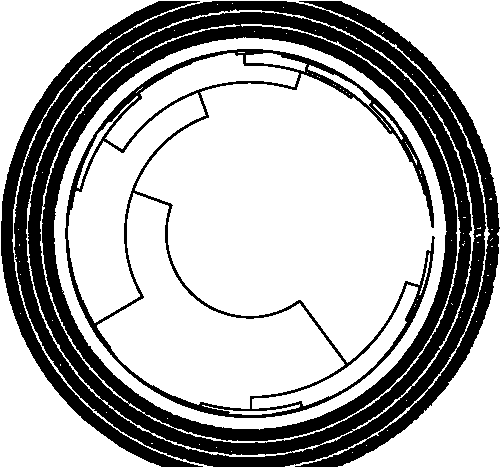
\includegraphics[width=1\textwidth,height=\textheight]{index_files/figure-pdf/unnamed-chunk-36-1.pdf}

}

\end{figure}

\begin{Shaded}
\begin{Highlighting}[]
\NormalTok{clust4\_MSA}\OtherTok{=}\FunctionTok{cutree}\NormalTok{(hc\_MSA,}\DecValTok{4}\NormalTok{)}
\FunctionTok{table}\NormalTok{(clust4\_MSA,meta\_taxo}\SpecialCharTok{$}\NormalTok{Kingdom)}
\end{Highlighting}
\end{Shaded}

\begin{verbatim}
          
clust4_MSA Animals Fungi Plants Protists
         1     331     0      0        0
         2     195     0      0        0
         3       9   154     14       56
         4       0     0    125        0
\end{verbatim}

\begin{Shaded}
\begin{Highlighting}[]
\NormalTok{aux}\OtherTok{=}\NormalTok{meta\_taxo }\SpecialCharTok{\%\textgreater{}\%} \FunctionTok{select}\NormalTok{(Organism,Kingdom,Phylum,Class,Full\_Name)}
\NormalTok{aux}\SpecialCharTok{$}\NormalTok{clust4\_MSA}\OtherTok{=}\NormalTok{clust4\_MSA}
\NormalTok{aux\_Animals\_cluster\_1\_2 }\OtherTok{=}\NormalTok{ aux }\SpecialCharTok{\%\textgreater{}\%} \FunctionTok{filter}\NormalTok{(Kingdom}\SpecialCharTok{==}\StringTok{"Animals"}\NormalTok{,clust4\_MSA }\SpecialCharTok{\%in\%} \FunctionTok{c}\NormalTok{(}\DecValTok{1}\NormalTok{,}\DecValTok{2}\NormalTok{))}
\FunctionTok{table}\NormalTok{(aux\_Animals\_cluster\_1\_2}\SpecialCharTok{$}\NormalTok{Phylum,aux\_Animals\_cluster\_1\_2}\SpecialCharTok{$}\NormalTok{clust4\_MSA)}
\end{Highlighting}
\end{Shaded}

\begin{verbatim}
                  
                     1   2
  Annelids           0   1
  Arthropods         0 158
  Brachiopodas       0   1
  Cephalochordates   0   2
  Cnidarians         0  10
  Echinoderms        0   3
  Hemichordates      0   1
  Mollusks           0  14
  Nematodes          0   1
  Placozoans         0   1
  Poriferans         0   1
  Tunicates          0   2
  Vertebrates      331   0
\end{verbatim}

\begin{Shaded}
\begin{Highlighting}[]
\NormalTok{aux\_9\_Animals\_cluster\_3}\OtherTok{=} \FunctionTok{filter}\NormalTok{(aux,clust4\_MSA}\SpecialCharTok{==}\DecValTok{3}\NormalTok{,Kingdom}\SpecialCharTok{==}\StringTok{"Animals"}\NormalTok{)}
\NormalTok{aux\_9\_Animals\_cluster\_3}
\end{Highlighting}
\end{Shaded}

\begin{verbatim}
# A tibble: 9 x 6
  Organism Kingdom Phylum    Class     Full_Name                      clust4_MSA
  <chr>    <chr>   <chr>     <chr>     <chr>                               <int>
1 bmy      Animals Nematodes Nematodes Brugia malayi (filaria)                 3
2 cbr      Animals Nematodes Nematodes Caenorhabditis briggsae (nema~          3
3 cel      Animals Nematodes Nematodes Caenorhabditis elegans (nemat~          3
4 loa      Animals Nematodes Nematodes Loa loa (eye worm)                      3
5 tsp      Animals Nematodes Nematodes Trichinella spiralis                    3
6 egl      Animals Flatworms Flatworms Echinococcus granulosus (hyda~          3
7 ovi      Animals Flatworms Flatworms Opisthorchis viverrini (South~          3
8 shx      Animals Flatworms Flatworms Schistosoma haematobium (urin~          3
9 smm      Animals Flatworms Flatworms Schistosoma mansoni                     3
\end{verbatim}

\begin{Shaded}
\begin{Highlighting}[]
\NormalTok{aux\_all\_Nematodes\_Flatworns}\OtherTok{=}\NormalTok{ aux }\SpecialCharTok{\%\textgreater{}\%} \FunctionTok{filter}\NormalTok{(Kingdom}\SpecialCharTok{==}\StringTok{"Animals"}\NormalTok{,Phylum }\SpecialCharTok{\%in\%} \FunctionTok{c}\NormalTok{(}\StringTok{"Nematodes"}\NormalTok{,}\StringTok{"Flatworms"}\NormalTok{))}
\NormalTok{aux\_all\_Nematodes\_Flatworns}
\end{Highlighting}
\end{Shaded}

\begin{verbatim}
# A tibble: 10 x 6
   Organism Kingdom Phylum    Class     Full_Name                     clust4_MSA
   <chr>    <chr>   <chr>     <chr>     <chr>                              <int>
 1 bmy      Animals Nematodes Nematodes Brugia malayi (filaria)                3
 2 cbr      Animals Nematodes Nematodes Caenorhabditis briggsae (nem~          3
 3 cel      Animals Nematodes Nematodes Caenorhabditis elegans (nema~          3
 4 loa      Animals Nematodes Nematodes Loa loa (eye worm)                     3
 5 nai      Animals Nematodes Nematodes Necator americanus (New Worl~          2
 6 tsp      Animals Nematodes Nematodes Trichinella spiralis                   3
 7 egl      Animals Flatworms Flatworms Echinococcus granulosus (hyd~          3
 8 ovi      Animals Flatworms Flatworms Opisthorchis viverrini (Sout~          3
 9 shx      Animals Flatworms Flatworms Schistosoma haematobium (uri~          3
10 smm      Animals Flatworms Flatworms Schistosoma mansoni                    3
\end{verbatim}

\begin{Shaded}
\begin{Highlighting}[]
\NormalTok{aux\_14\_Plants\_clust2}\OtherTok{=} \FunctionTok{filter}\NormalTok{(aux,clust4\_MSA}\SpecialCharTok{==}\DecValTok{3}\NormalTok{,Kingdom}\SpecialCharTok{==}\StringTok{"Plants"}\NormalTok{)}
\NormalTok{aux\_14\_Plants\_clust2}
\end{Highlighting}
\end{Shaded}

\begin{verbatim}
# A tibble: 14 x 6
   Organism Kingdom Phylum Class Full_Name                      clust4_MSA
   <chr>    <chr>   <chr>  <chr> <chr>                               <int>
 1 apro     Plants  Green  algae Auxenochlorella protothecoides          3
 2 bpg      Plants  Green  algae Bathycoccus prasinos                    3
 3 cre      Plants  Green  algae Chlamydomonas reinhardtii               3
 4 csl      Plants  Green  algae Coccomyxa subellipsoidea                3
 5 cvr      Plants  Green  algae Chlorella variabilis                    3
 6 mis      Plants  Green  algae Micromonas commoda                      3
 7 mng      Plants  Green  algae Monoraphidium neglectum                 3
 8 mpp      Plants  Green  algae Micromonas pusilla                      3
 9 olu      Plants  Green  algae Ostreococcus lucimarinus                3
10 ota      Plants  Green  algae Ostreococcus tauri                      3
11 vcn      Plants  Green  algae Volvox carteri f. nagariensis           3
12 ccp      Plants  Red    algae Chondrus crispus (carragheen)           3
13 cme      Plants  Red    algae Cyanidioschyzon merolae                 3
14 gsl      Plants  Red    algae Galdieria sulphuraria                   3
\end{verbatim}

\begin{Shaded}
\begin{Highlighting}[]
\NormalTok{aux\_all\_algae\_class}\OtherTok{=}\NormalTok{ aux }\SpecialCharTok{\%\textgreater{}\%} \FunctionTok{filter}\NormalTok{(Kingdom}\SpecialCharTok{==}\StringTok{"Plants"}\NormalTok{,Class }\SpecialCharTok{\%in\%} \FunctionTok{c}\NormalTok{(}\StringTok{"algae"}\NormalTok{))}
\NormalTok{aux\_all\_algae\_class}
\end{Highlighting}
\end{Shaded}

\begin{verbatim}
# A tibble: 14 x 6
   Organism Kingdom Phylum Class Full_Name                      clust4_MSA
   <chr>    <chr>   <chr>  <chr> <chr>                               <int>
 1 apro     Plants  Green  algae Auxenochlorella protothecoides          3
 2 bpg      Plants  Green  algae Bathycoccus prasinos                    3
 3 cre      Plants  Green  algae Chlamydomonas reinhardtii               3
 4 csl      Plants  Green  algae Coccomyxa subellipsoidea                3
 5 cvr      Plants  Green  algae Chlorella variabilis                    3
 6 mis      Plants  Green  algae Micromonas commoda                      3
 7 mng      Plants  Green  algae Monoraphidium neglectum                 3
 8 mpp      Plants  Green  algae Micromonas pusilla                      3
 9 olu      Plants  Green  algae Ostreococcus lucimarinus                3
10 ota      Plants  Green  algae Ostreococcus tauri                      3
11 vcn      Plants  Green  algae Volvox carteri f. nagariensis           3
12 ccp      Plants  Red    algae Chondrus crispus (carragheen)           3
13 cme      Plants  Red    algae Cyanidioschyzon merolae                 3
14 gsl      Plants  Red    algae Galdieria sulphuraria                   3
\end{verbatim}

The hierarchical classification by Ward's method recovers the kingdom
Animal clusters 1 (all vertebrates) and 2 (invertebrate animals),
cluster 4 the Plants and in cluster 3 are all protists and fungi
together with 9 animals and 14 plants.

The 9 Animals are all from the Phylum Nematodes or Flatworns, out of the
total of the 10 species of these phylums considered in the experiment.
Only the Nematode Necator americanus (New World hookworm) is classified
in Animals.

The 14 plants in cluster 2 are all algae considered in the experiment.

\hypertarget{mds-multidimensional-scaling-munkres}{%
\section{MDS (Multidimensional Scaling)
Munkres}\label{mds-multidimensional-scaling-munkres}}

\begin{Shaded}
\begin{Highlighting}[]
\DocumentationTok{\#\# Metric multidimensional scaling}
\NormalTok{mds7 }\OtherTok{\textless{}{-}} \FunctionTok{cmdscale}\NormalTok{(}\FunctionTok{sqrt}\NormalTok{(}\DecValTok{1}\SpecialCharTok{{-}}\NormalTok{Sim\_Mun\_mDAG}\SpecialCharTok{\^{}}\DecValTok{2}\NormalTok{),}\AttributeTok{k=}\DecValTok{7}\NormalTok{,}\AttributeTok{eig=}\ConstantTok{TRUE}\NormalTok{)}
\NormalTok{mds7}\SpecialCharTok{$}\NormalTok{GOF}
\end{Highlighting}
\end{Shaded}

\begin{verbatim}
[1] 0.5600385 0.5796647
\end{verbatim}

\begin{Shaded}
\begin{Highlighting}[]
\NormalTok{mds }\OtherTok{\textless{}{-}}\NormalTok{ mds7}\SpecialCharTok{$}\NormalTok{points }\SpecialCharTok{\%\textgreater{}\%}  \FunctionTok{as\_tibble}\NormalTok{()}
\FunctionTok{colnames}\NormalTok{(mds) }\OtherTok{\textless{}{-}}\FunctionTok{paste0}\NormalTok{(}\StringTok{"Dim."}\NormalTok{,}\DecValTok{1}\SpecialCharTok{:}\FunctionTok{dim}\NormalTok{(mds7}\SpecialCharTok{$}\NormalTok{points)[}\DecValTok{2}\NormalTok{])}

\NormalTok{cooordinates}\OtherTok{=}\FunctionTok{as\_tibble}\NormalTok{(mds7}\SpecialCharTok{$}\NormalTok{points)}
\FunctionTok{colnames}\NormalTok{(cooordinates)}\OtherTok{=}\FunctionTok{paste}\NormalTok{(}\StringTok{"Component"}\NormalTok{,}\DecValTok{1}\SpecialCharTok{:}\DecValTok{7}\NormalTok{)}
\FunctionTok{ggpairs}\NormalTok{(cooordinates,}\AttributeTok{columns=}\DecValTok{1}\SpecialCharTok{:}\DecValTok{4}\NormalTok{,}
        \FunctionTok{aes}\NormalTok{(}\AttributeTok{color=}\NormalTok{meta\_taxo}\SpecialCharTok{$}\NormalTok{Kingdom,}
            \AttributeTok{title=}\StringTok{"MDS 4 dimensions projection"}\NormalTok{,}\AttributeTok{legend=}\DecValTok{1}\NormalTok{),}
        \AttributeTok{lower=}\FunctionTok{list}\NormalTok{(}\AttributeTok{continuous=}\StringTok{"points"}\NormalTok{)) }\SpecialCharTok{+} 
  \FunctionTok{scale\_fill\_manual}\NormalTok{(}\AttributeTok{values =}\NormalTok{ colorsK}\SpecialCharTok{$}\NormalTok{Kingdom) }\SpecialCharTok{+} 
  \FunctionTok{theme}\NormalTok{(}\AttributeTok{legend.position =} \StringTok{"left"}\NormalTok{)}
\end{Highlighting}
\end{Shaded}

\begin{figure}[H]

{\centering 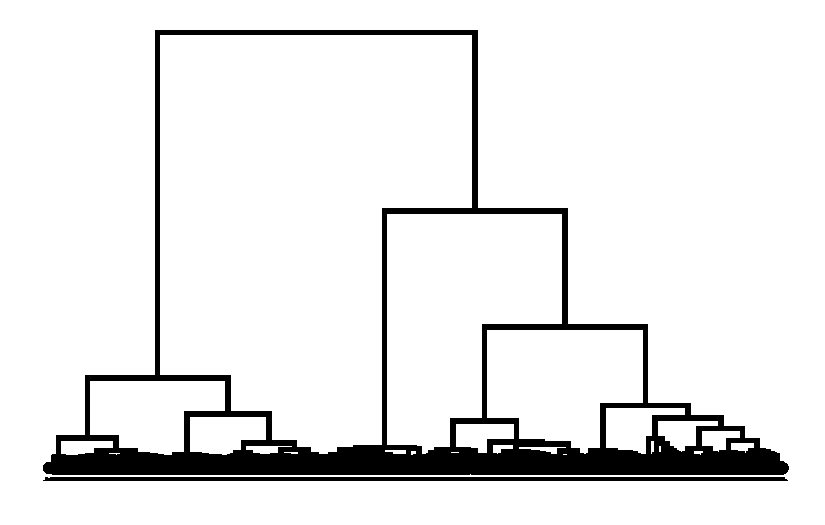
\includegraphics[width=1\textwidth,height=\textheight]{index_files/figure-pdf/unnamed-chunk-39-1.pdf}

}

\end{figure}

\hypertarget{hierarchical-cluster-munkres}{%
\section{Hierarchical cluster
Munkres}\label{hierarchical-cluster-munkres}}

\begin{Shaded}
\begin{Highlighting}[]
\NormalTok{D}\OtherTok{=}\FunctionTok{as.dist}\NormalTok{(}\FunctionTok{sqrt}\NormalTok{(}\DecValTok{1}\SpecialCharTok{{-}}\NormalTok{Sim\_Mun\_mDAG}\SpecialCharTok{\^{}}\DecValTok{2}\NormalTok{))}
\NormalTok{hc}\OtherTok{=}\FunctionTok{hclust}\NormalTok{(}\FunctionTok{as.dist}\NormalTok{(D),}\AttributeTok{method =}\StringTok{"ward.D"}\NormalTok{)}
\FunctionTok{ggplot}\NormalTok{(}\FunctionTok{as.ggdend}\NormalTok{(}\FunctionTok{as.dendrogram}\NormalTok{(hc)))}
\end{Highlighting}
\end{Shaded}

\begin{figure}[H]

{\centering 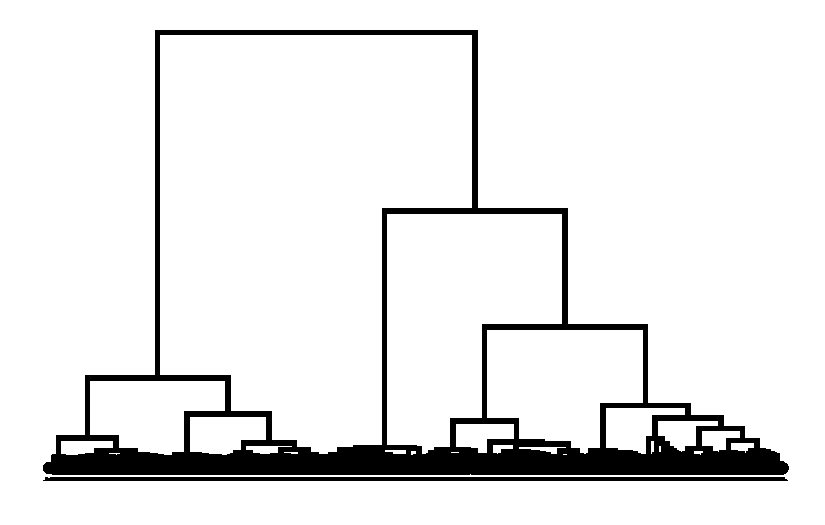
\includegraphics[width=1\textwidth,height=\textheight]{index_files/figure-pdf/unnamed-chunk-40-1.pdf}

}

\end{figure}

\begin{Shaded}
\begin{Highlighting}[]
\NormalTok{clust4}\OtherTok{=}\FunctionTok{cutree}\NormalTok{(hc,}\DecValTok{4}\NormalTok{)}
\FunctionTok{table}\NormalTok{(clust4,meta\_taxo}\SpecialCharTok{$}\NormalTok{Kingdom)}
\end{Highlighting}
\end{Shaded}

\begin{verbatim}
      
clust4 Animals Fungi Plants Protists
     1     331     0      0        0
     2     197     0      0        0
     3       7   154     14       56
     4       0     0    125        0
\end{verbatim}

\hypertarget{similarity-comparison-eukaryotes}{%
\section{Similarity comparison
Eukaryotes}\label{similarity-comparison-eukaryotes}}

Comparison of two similarities

Load the similarities for pairs and comparison

\begin{Shaded}
\begin{Highlighting}[]
\NormalTok{n}\OtherTok{=}\FunctionTok{length}\NormalTok{(meta\_taxo}\SpecialCharTok{$}\NormalTok{mDAG\_Id)}
\NormalTok{n}
\end{Highlighting}
\end{Shaded}

\begin{verbatim}
[1] 884
\end{verbatim}

\begin{Shaded}
\begin{Highlighting}[]
\FunctionTok{dim}\NormalTok{(Sim\_MSA\_mDAG)}
\end{Highlighting}
\end{Shaded}

\begin{verbatim}
[1] 884 884
\end{verbatim}

\begin{Shaded}
\begin{Highlighting}[]
\CommentTok{\#aux1=base::rep(x=1:n,each=c(n:1))}

\NormalTok{aux}\OtherTok{=}\FunctionTok{as\_tibble}\NormalTok{(Sim\_MSA\_mDAG)}
\NormalTok{aux}\SpecialCharTok{$}\NormalTok{mDag}\OtherTok{=}\FunctionTok{names}\NormalTok{(aux)}
\NormalTok{aux}\OtherTok{=}\NormalTok{aux }\SpecialCharTok{\%\textgreater{}\%} \FunctionTok{pivot\_longer}\NormalTok{(}\AttributeTok{cols=}\StringTok{\textasciigrave{}}\AttributeTok{0313}\StringTok{\textasciigrave{}}\SpecialCharTok{:}\StringTok{\textasciigrave{}}\AttributeTok{0300}\StringTok{\textasciigrave{}}\NormalTok{,}
                         \AttributeTok{names\_to=}\StringTok{"mDag\_2"}\NormalTok{,}
                         \AttributeTok{values\_to=}\StringTok{"Sim\_MSA"}\NormalTok{)}

\NormalTok{aux\_2}\OtherTok{=}\NormalTok{ aux }\SpecialCharTok{\%\textgreater{}\%}  \FunctionTok{mutate}\NormalTok{(}\AttributeTok{i=}\FunctionTok{pmax}\NormalTok{(}\FunctionTok{as.integer}\NormalTok{(mDag),}
                              \FunctionTok{as.integer}\NormalTok{(mDag\_2)),}
                       \AttributeTok{j=}\FunctionTok{pmin}\NormalTok{(}\FunctionTok{as.integer}\NormalTok{(mDag),}
                       \FunctionTok{as.integer}\NormalTok{(mDag\_2))) }\SpecialCharTok{\%\textgreater{}\%} \FunctionTok{unite}\NormalTok{(}\StringTok{"ij"}\NormalTok{,i}\SpecialCharTok{:}\NormalTok{j) }\SpecialCharTok{\%\textgreater{}\%}
  \FunctionTok{filter}\NormalTok{(}\FunctionTok{duplicated}\NormalTok{(ij))}


\NormalTok{aux}\OtherTok{=}\FunctionTok{as\_tibble}\NormalTok{(Sim\_Mun\_mDAG)}
\NormalTok{aux}\SpecialCharTok{$}\NormalTok{mDag}\OtherTok{=}\FunctionTok{names}\NormalTok{(aux)}
\NormalTok{aux}\OtherTok{=}\NormalTok{aux }\SpecialCharTok{\%\textgreater{}\%} \FunctionTok{pivot\_longer}\NormalTok{(}\AttributeTok{cols=}\StringTok{\textasciigrave{}}\AttributeTok{0313}\StringTok{\textasciigrave{}}\SpecialCharTok{:}\StringTok{\textasciigrave{}}\AttributeTok{0300}\StringTok{\textasciigrave{}}\NormalTok{,}
                         \AttributeTok{names\_to=}\StringTok{"mDag\_2"}\NormalTok{,}
                         \AttributeTok{values\_to=}\StringTok{"Sim\_Mun"}\NormalTok{)}
\NormalTok{aux\_2 }\OtherTok{=}\NormalTok{ aux\_2 }\SpecialCharTok{\%\textgreater{}\%} \FunctionTok{left\_join}\NormalTok{(aux)}

\NormalTok{Sim\_comp}\OtherTok{=}\NormalTok{aux\_2}
\FunctionTok{rm}\NormalTok{(aux,aux\_2)}
\end{Highlighting}
\end{Shaded}

\textbf{Spearman and Pearson correlations}

\begin{Shaded}
\begin{Highlighting}[]
\FunctionTok{cor}\NormalTok{(Sim\_comp[,}\FunctionTok{c}\NormalTok{(}\DecValTok{3}\NormalTok{,}\DecValTok{5}\NormalTok{)],}\AttributeTok{method=}\StringTok{"spearman"}\NormalTok{)}
\end{Highlighting}
\end{Shaded}

\begin{verbatim}
          Sim_MSA   Sim_Mun
Sim_MSA 1.0000000 0.8902053
Sim_Mun 0.8902053 1.0000000
\end{verbatim}

\begin{Shaded}
\begin{Highlighting}[]
\FunctionTok{cor}\NormalTok{(Sim\_comp[,}\FunctionTok{c}\NormalTok{(}\DecValTok{3}\NormalTok{,}\DecValTok{5}\NormalTok{)],}\AttributeTok{method=}\StringTok{"pearson"}\NormalTok{)}
\end{Highlighting}
\end{Shaded}

\begin{verbatim}
          Sim_MSA   Sim_Mun
Sim_MSA 1.0000000 0.9138905
Sim_Mun 0.9138905 1.0000000
\end{verbatim}

\begin{Shaded}
\begin{Highlighting}[]
\NormalTok{GGally}\SpecialCharTok{::}\FunctionTok{ggpairs}\NormalTok{(Sim\_comp[,}\FunctionTok{c}\NormalTok{(}\DecValTok{3}\NormalTok{,}\DecValTok{5}\NormalTok{)])}
\end{Highlighting}
\end{Shaded}

\begin{figure}[H]

{\centering 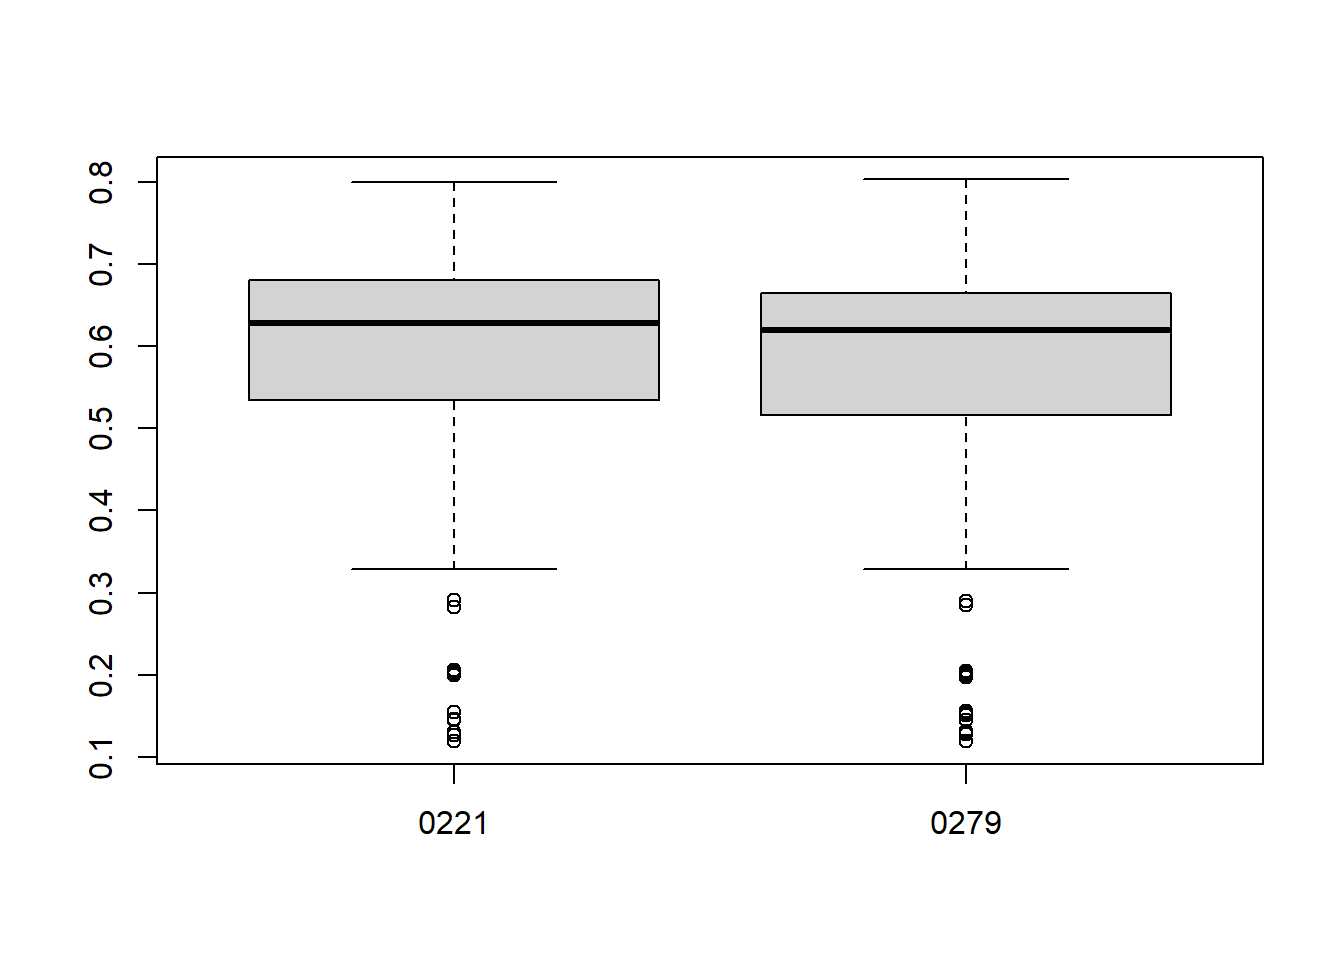
\includegraphics[width=1\textwidth,height=\textheight]{index_files/figure-pdf/unnamed-chunk-44-1.pdf}

}

\end{figure}

\begin{Shaded}
\begin{Highlighting}[]
\NormalTok{aux}\OtherTok{=}\NormalTok{ Sim\_comp}\SpecialCharTok{\%\textgreater{}\%} \FunctionTok{pivot\_longer}\NormalTok{(}
  \AttributeTok{cols=}\FunctionTok{c}\NormalTok{(Sim\_MSA,Sim\_Mun),            }\AttributeTok{names\_to=}\StringTok{"Method"}\NormalTok{,}
  \AttributeTok{values\_to=}\StringTok{"Similarity"}\NormalTok{)}

\NormalTok{ggstatsplot}\SpecialCharTok{::}\FunctionTok{ggbetweenstats}\NormalTok{(}
  \AttributeTok{data =}\NormalTok{ aux,}
  \AttributeTok{x =}\NormalTok{ Method,}
  \AttributeTok{y =}\NormalTok{ Similarity)}
\end{Highlighting}
\end{Shaded}

\begin{figure}[H]

{\centering 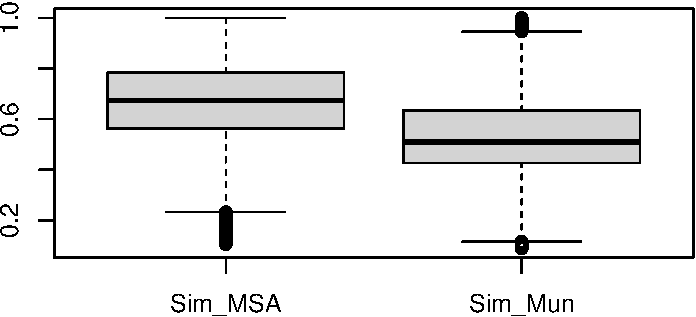
\includegraphics[width=1\textwidth,height=\textheight]{index_files/figure-pdf/unnamed-chunk-45-1.pdf}

}

\end{figure}

\bookmarksetup{startatroot}

\hypertarget{graph}{%
\chapter{Graph}\label{graph}}

Some statistics for graphs

\hypertarget{read-all-graphs-from-a-level-of-the-experiment}{%
\section{Read all graphs from a level of the
experiment}\label{read-all-graphs-from-a-level-of-the-experiment}}

Read all graphs from a level from experiment; for example individuals.
We read only firts (alphabetic) two graph

\begin{Shaded}
\begin{Highlighting}[]
\NormalTok{path\_exp}\OtherTok{=}\StringTok{"data/result\_bb261b6e{-}95c6{-}3e39{-}b82b{-}b68eea80e30b/data/"}
\NormalTok{list\_names}\OtherTok{=}\FunctionTok{dir}\NormalTok{(}\FunctionTok{paste0}\NormalTok{(path\_exp,}\StringTok{"Individuals/"}\NormalTok{))}

\NormalTok{list\_names}\OtherTok{=}\NormalTok{ list\_names[}\SpecialCharTok{{-}}\DecValTok{1}\NormalTok{] }\CommentTok{\# filter 0000\_RefPw}
\FunctionTok{length}\NormalTok{(list\_names)}
\end{Highlighting}
\end{Shaded}

\begin{verbatim}
[1] 884
\end{verbatim}

\begin{Shaded}
\begin{Highlighting}[]
\NormalTok{graphs\_list}\OtherTok{=}\FunctionTok{paste0}\NormalTok{(path\_exp,}\StringTok{"Individuals/"}\NormalTok{,list\_names,}\StringTok{"/"}\NormalTok{,list\_names,}\StringTok{"\_MDAG.graphml"}\NormalTok{)}
\end{Highlighting}
\end{Shaded}

RRRRRRRRRRRRRRRRRRRRRRRRRRRRR

\begin{Shaded}
\begin{Highlighting}[]
\CommentTok{\#knitr::include\_graphics(paste0(path\_exp,"Individuals/cang/cang\_mDAG\_essential.pdf"))}
\end{Highlighting}
\end{Shaded}

\begin{Shaded}
\begin{Highlighting}[]
\CommentTok{\#knitr::include\_graphics(paste0(path\_exp,"Individuals/cang/cang\_mDAG\_essential.pdf"))}
\end{Highlighting}
\end{Shaded}

\begin{Shaded}
\begin{Highlighting}[]
\NormalTok{knitr}\SpecialCharTok{::}\FunctionTok{include\_graphics}\NormalTok{(}
  \FunctionTok{paste0}\NormalTok{(path\_exp,}\StringTok{"Individuals/cang/cang\_RC.pdf"}\NormalTok{))}
\end{Highlighting}
\end{Shaded}

\begin{figure}[H]

{\centering \includegraphics[width=1\textwidth,height=\textheight]{data/result_bb261b6e-95c6-3e39-b82b-b68eea80e30b/data/Individuals/cang/cang_RC.pdf}

}

\end{figure}

\hypertarget{graph-statistics}{%
\section{Graph statistics}\label{graph-statistics}}

\begin{Shaded}
\begin{Highlighting}[]
\NormalTok{read\_mDAG}\OtherTok{=}\ControlFlowTok{function}\NormalTok{(x) \{DAG}\OtherTok{=}\FunctionTok{read.graph}\NormalTok{(}\AttributeTok{file=}\NormalTok{x,}
                                  \AttributeTok{format=}\StringTok{"graphml"}\NormalTok{)}
  \FunctionTok{return}\NormalTok{(DAG)\}}
\NormalTok{mDAG\_componets}\OtherTok{=}\ControlFlowTok{function}\NormalTok{(x) \{}\FunctionTok{sort}\NormalTok{(}\FunctionTok{components}\NormalTok{(x,}\AttributeTok{mode =} \StringTok{"weak"}\NormalTok{)}\SpecialCharTok{$}\NormalTok{csize,}
                                 \AttributeTok{decreasing=}\ConstantTok{TRUE}\NormalTok{)\}}



\NormalTok{compo\_list}\OtherTok{=}\FunctionTok{lapply}\NormalTok{(graphs\_list,}
                  \AttributeTok{FUN=}\ControlFlowTok{function}\NormalTok{(x) \{}
\NormalTok{                    gg}\OtherTok{=}\FunctionTok{read\_mDAG}\NormalTok{(x)}
\NormalTok{                  aux}\OtherTok{=}\FunctionTok{list}\NormalTok{(}
                    \AttributeTok{mDAG\_componets=}\FunctionTok{mDAG\_componets}\NormalTok{(gg),}
                    \AttributeTok{degree\_count=}\NormalTok{igraph}\SpecialCharTok{::}\FunctionTok{degree}\NormalTok{(gg,}\AttributeTok{mode=}\StringTok{"total"}\NormalTok{))}
                    \FunctionTok{return}\NormalTok{(aux)\}}
\NormalTok{                  )}

\FunctionTok{names}\NormalTok{(compo\_list)}\OtherTok{=}\NormalTok{list\_names}
\NormalTok{n}\OtherTok{=}\FunctionTok{max}\NormalTok{(}\FunctionTok{sapply}\NormalTok{(compo\_list,}\AttributeTok{FUN=}\ControlFlowTok{function}\NormalTok{(x) \{}\FunctionTok{length}\NormalTok{(x[[}\DecValTok{1}\NormalTok{]])\}))}
\NormalTok{n}
\end{Highlighting}
\end{Shaded}

\begin{verbatim}
[1] 234
\end{verbatim}

\begin{Shaded}
\begin{Highlighting}[]
\NormalTok{size\_compo\_list}\OtherTok{=}\FunctionTok{lapply}\NormalTok{(compo\_list,}\AttributeTok{FUN=}\ControlFlowTok{function}\NormalTok{(x) \{}
  \FunctionTok{return}\NormalTok{(}\FunctionTok{c}\NormalTok{(x[[}\DecValTok{1}\NormalTok{]],}\FunctionTok{rep}\NormalTok{(}\ConstantTok{NA}\NormalTok{,n}\SpecialCharTok{{-}}\FunctionTok{length}\NormalTok{(x[[}\DecValTok{1}\NormalTok{]]))))\})}

\NormalTok{aux}\OtherTok{=}\FunctionTok{do.call}\NormalTok{(bind\_cols,size\_compo\_list)}
\NormalTok{aux2}\OtherTok{=}\FunctionTok{pivot\_longer}\NormalTok{(aux,aaf}\SpecialCharTok{:}\NormalTok{zvi,}\AttributeTok{names\_to=}\StringTok{"Organism"}\NormalTok{,}
                  \AttributeTok{values\_to=}\StringTok{"csize"}\NormalTok{)}\SpecialCharTok{\%\textgreater{}\%}
  \FunctionTok{arrange}\NormalTok{(Organism,}\SpecialCharTok{{-}}\NormalTok{csize)}
\NormalTok{aux2}\SpecialCharTok{$}\NormalTok{index}\OtherTok{=}\FunctionTok{rep}\NormalTok{(}\DecValTok{1}\SpecialCharTok{:}\NormalTok{n,}\AttributeTok{times=}\FunctionTok{dim}\NormalTok{(aux)[}\DecValTok{2}\NormalTok{])}
\NormalTok{aux2}\OtherTok{=}\NormalTok{aux2 }\SpecialCharTok{\%\textgreater{}\%} \FunctionTok{left\_join}\NormalTok{(meta\_taxo,}\AttributeTok{by=}\StringTok{"Organism"}\NormalTok{)}
\end{Highlighting}
\end{Shaded}

\begin{Shaded}
\begin{Highlighting}[]
\NormalTok{Organism}\OtherTok{=}\FunctionTok{names}\NormalTok{(compo\_list)}
\NormalTok{big\_MBB}\OtherTok{=}\ControlFlowTok{function}\NormalTok{(org)\{}
\NormalTok{  x}\OtherTok{=}\NormalTok{Results }\SpecialCharTok{\%\textgreater{}\%} \FunctionTok{filter}\NormalTok{(Organism}\SpecialCharTok{==}\NormalTok{org)}
\NormalTok{  x}\OtherTok{=}\FunctionTok{as.character}\NormalTok{(x[}\DecValTok{1}\NormalTok{,}\DecValTok{5}\SpecialCharTok{:}\FunctionTok{dim}\NormalTok{(Results)[}\DecValTok{2}\NormalTok{]])}
\NormalTok{  x}\OtherTok{=}\NormalTok{x[x}\SpecialCharTok{!=}\StringTok{"NA"}\NormalTok{]}
\NormalTok{  tt}\OtherTok{=}\FunctionTok{sort}\NormalTok{(}\FunctionTok{table}\NormalTok{(x),}\AttributeTok{decreasing=}\ConstantTok{TRUE}\NormalTok{)}
  \FunctionTok{return}\NormalTok{(tt)}
\NormalTok{  \}}
\NormalTok{big\_MBB\_list}\OtherTok{=} \FunctionTok{lapply}\NormalTok{(Organism,}\AttributeTok{FUN=}\ControlFlowTok{function}\NormalTok{(x) }\FunctionTok{big\_MBB}\NormalTok{(x))}
\NormalTok{nMBB}\OtherTok{=}\FunctionTok{max}\NormalTok{(}\FunctionTok{sapply}\NormalTok{(big\_MBB\_list,}\AttributeTok{FUN=}\ControlFlowTok{function}\NormalTok{(x) }\FunctionTok{length}\NormalTok{(x)))}
\NormalTok{nMBB}
\end{Highlighting}
\end{Shaded}

\begin{verbatim}
[1] 1041
\end{verbatim}

\begin{Shaded}
\begin{Highlighting}[]
\NormalTok{big\_MBB\_list}\OtherTok{=}\FunctionTok{lapply}\NormalTok{(big\_MBB\_list,}
                    \AttributeTok{FUN=}\ControlFlowTok{function}\NormalTok{(x)\{}
\NormalTok{                      x}\OtherTok{=}\FunctionTok{c}\NormalTok{(x,}\FunctionTok{rep}\NormalTok{(}\ConstantTok{NA}\NormalTok{,nMBB}\SpecialCharTok{{-}}\FunctionTok{length}\NormalTok{(x)))}
                      \FunctionTok{return}\NormalTok{(x)\}}
\NormalTok{)}
\FunctionTok{names}\NormalTok{(big\_MBB\_list)}\OtherTok{=}\NormalTok{Organism}
\NormalTok{big\_MBB\_list}\OtherTok{=}\FunctionTok{do.call}\NormalTok{(bind\_cols,big\_MBB\_list)}

\NormalTok{kMBB}\OtherTok{=}\FunctionTok{nrow}\NormalTok{(big\_MBB\_list)}
\NormalTok{index}\OtherTok{=}\FunctionTok{rep}\NormalTok{(}\DecValTok{1}\SpecialCharTok{:}\NormalTok{kMBB,}\AttributeTok{times=}\FunctionTok{length}\NormalTok{(Organism))}

\NormalTok{big\_MBB\_list2}\OtherTok{=}\FunctionTok{pivot\_longer}\NormalTok{(big\_MBB\_list,}\AttributeTok{cols=}\FunctionTok{names}\NormalTok{(big\_MBB\_list),}\AttributeTok{values\_to =} \StringTok{"MBBsize"}\NormalTok{,}\AttributeTok{names\_to =} \StringTok{"Organism"}\NormalTok{) }\SpecialCharTok{\%\textgreater{}\%} \FunctionTok{arrange}\NormalTok{(Organism,}\SpecialCharTok{{-}}\NormalTok{MBBsize)}\SpecialCharTok{\%\textgreater{}\%}  \FunctionTok{mutate}\NormalTok{(}\AttributeTok{index=}\NormalTok{index) }\SpecialCharTok{\%\textgreater{}\%}  \FunctionTok{left\_join}\NormalTok{(meta\_taxo,}\AttributeTok{by=}\StringTok{"Organism"}\NormalTok{)}
\end{Highlighting}
\end{Shaded}

\hypertarget{sizes-of-mbb-for-each-mdag}{%
\subsection{Sizes of MBB for each
mDAG}\label{sizes-of-mbb-for-each-mdag}}

\begin{Shaded}
\begin{Highlighting}[]
\NormalTok{COLOR\_KINGDOM}\OtherTok{=}\FunctionTok{c}\NormalTok{(}\StringTok{"red"}\NormalTok{,}\StringTok{"green"}\NormalTok{,}\StringTok{"yellow"}\NormalTok{,}\StringTok{"black"}\NormalTok{)}
\NormalTok{colors\_kingdom}\OtherTok{=}\NormalTok{big\_MBB\_list2}\SpecialCharTok{\%\textgreater{}\%} \FunctionTok{select}\NormalTok{(Organism,Kingdom) }\SpecialCharTok{\%\textgreater{}\%} \FunctionTok{distinct}\NormalTok{()}
\FunctionTok{names}\NormalTok{(COLOR\_KINGDOM)}\OtherTok{=}\FunctionTok{sort}\NormalTok{(}\FunctionTok{unique}\NormalTok{(colors\_kingdom}\SpecialCharTok{$}\NormalTok{Kingdom))}

\NormalTok{p0}\OtherTok{\textless{}{-}}\FunctionTok{ggplot}\NormalTok{(}\AttributeTok{data=}\NormalTok{big\_MBB\_list2) }\SpecialCharTok{+} 
  \FunctionTok{geom\_line}\NormalTok{(}\AttributeTok{mapping=}\FunctionTok{aes}\NormalTok{(}\AttributeTok{x=}\NormalTok{index,}\AttributeTok{y=}\NormalTok{MBBsize,}\AttributeTok{group =}\NormalTok{ Organism,}\AttributeTok{color=}\NormalTok{Kingdom)) }\SpecialCharTok{+} 
  \FunctionTok{scale\_y\_continuous}\NormalTok{(}\AttributeTok{trans=}\StringTok{\textquotesingle{}log10\textquotesingle{}}\NormalTok{) }\SpecialCharTok{+} 
  \FunctionTok{scale\_x\_continuous}\NormalTok{(}\AttributeTok{trans=}\StringTok{\textquotesingle{}identity\textquotesingle{}}\NormalTok{) }\SpecialCharTok{+}
  \FunctionTok{scale\_color\_manual}\NormalTok{(}\AttributeTok{values =}\NormalTok{COLOR\_KINGDOM[colors\_kingdom}\SpecialCharTok{$}\NormalTok{Kingdom])}\SpecialCharTok{+}
   \FunctionTok{ggtitle}\NormalTok{(}\StringTok{"Plot log{-}identity of MBB }\SpecialCharTok{\textbackslash{}n}\StringTok{  decreasing index."}\NormalTok{) }\SpecialCharTok{+}
  \FunctionTok{ylab}\NormalTok{(}\StringTok{"Log10 MBB size"}\NormalTok{) }\SpecialCharTok{+} \FunctionTok{xlab}\NormalTok{(}\StringTok{"Index"}\NormalTok{)}


\NormalTok{p1}\OtherTok{\textless{}{-}} \FunctionTok{ggplot}\NormalTok{(}\AttributeTok{data=}\NormalTok{big\_MBB\_list2) }\SpecialCharTok{+} 
  \FunctionTok{geom\_line}\NormalTok{(}\AttributeTok{mapping=}\FunctionTok{aes}\NormalTok{(}\AttributeTok{x=}\NormalTok{index,}\AttributeTok{y=}\NormalTok{MBBsize,}\AttributeTok{group =}\NormalTok{ Organism,}\AttributeTok{color=}\NormalTok{Kingdom),}\AttributeTok{na.rm=}\ConstantTok{TRUE}\NormalTok{) }\SpecialCharTok{+} 
  \FunctionTok{scale\_x\_continuous}\NormalTok{(}\AttributeTok{trans=}\StringTok{\textquotesingle{}log10\textquotesingle{}}\NormalTok{) }\SpecialCharTok{+} 
  \FunctionTok{scale\_y\_continuous}\NormalTok{(}\AttributeTok{trans=}\StringTok{\textquotesingle{}log10\textquotesingle{}}\NormalTok{) }\SpecialCharTok{+}
  \FunctionTok{scale\_color\_manual}\NormalTok{(}\AttributeTok{values =}\NormalTok{COLOR\_KINGDOM[colors\_kingdom}\SpecialCharTok{$}\NormalTok{Kingdom])}\SpecialCharTok{+}
   \FunctionTok{ggtitle}\NormalTok{(}\StringTok{"Plot log10{-}log10identity of MBB }\SpecialCharTok{\textbackslash{}n}\StringTok{  decreasing index."}\NormalTok{) }\SpecialCharTok{+}
  \FunctionTok{ylab}\NormalTok{(}\StringTok{"Log10 MBB size"}\NormalTok{) }\SpecialCharTok{+} \FunctionTok{xlab}\NormalTok{(}\StringTok{"Log10 Index"}\NormalTok{)}

\NormalTok{p2}\OtherTok{\textless{}{-}} \FunctionTok{ggplot}\NormalTok{(}\AttributeTok{data=}\NormalTok{big\_MBB\_list2) }\SpecialCharTok{+} 
  \FunctionTok{geom\_line}\NormalTok{(}\AttributeTok{mapping=}\FunctionTok{aes}\NormalTok{(}\AttributeTok{x=}\NormalTok{index,}\AttributeTok{y=}\NormalTok{MBBsize,}\AttributeTok{group =}\NormalTok{ Organism,}\AttributeTok{color=}\NormalTok{Kingdom),}\AttributeTok{na.rm=}\ConstantTok{TRUE}\NormalTok{)}\SpecialCharTok{+}
   \FunctionTok{scale\_x\_continuous}\NormalTok{(}\AttributeTok{trans=}\StringTok{"identity"}\NormalTok{) }\SpecialCharTok{+} 
   \FunctionTok{scale\_y\_continuous}\NormalTok{(}\AttributeTok{trans=}\StringTok{"identity"}\NormalTok{) }\SpecialCharTok{+}
  \FunctionTok{ylim}\NormalTok{(}\DecValTok{0}\NormalTok{,}\DecValTok{1039}\NormalTok{)}\SpecialCharTok{+}
   \FunctionTok{ggtitle}\NormalTok{(}\StringTok{"Plot  of MBB sized  decreasing index."}\NormalTok{) }\SpecialCharTok{+}
  \FunctionTok{ylab}\NormalTok{(}\StringTok{"MBB size"}\NormalTok{) }\SpecialCharTok{+} \FunctionTok{xlab}\NormalTok{(}\StringTok{"Index"}\NormalTok{)}\SpecialCharTok{+}
  \FunctionTok{scale\_color\_manual}\NormalTok{(}\AttributeTok{values =}\NormalTok{COLOR\_KINGDOM[colors\_kingdom}\SpecialCharTok{$}\NormalTok{Kingdom])}


\NormalTok{p0}
\end{Highlighting}
\end{Shaded}

\begin{figure}[H]

{\centering 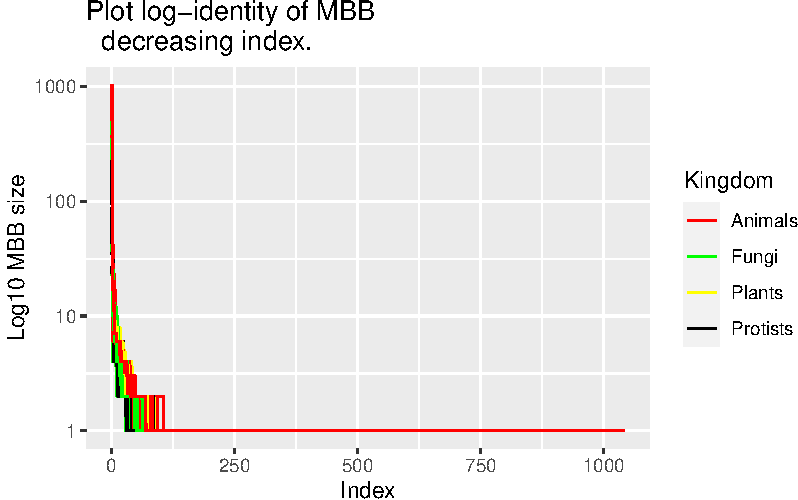
\includegraphics[width=1\textwidth,height=\textheight]{index_files/figure-pdf/unnamed-chunk-52-1.pdf}

}

\end{figure}

\begin{Shaded}
\begin{Highlighting}[]
\NormalTok{p1}
\end{Highlighting}
\end{Shaded}

\begin{figure}[H]

{\centering 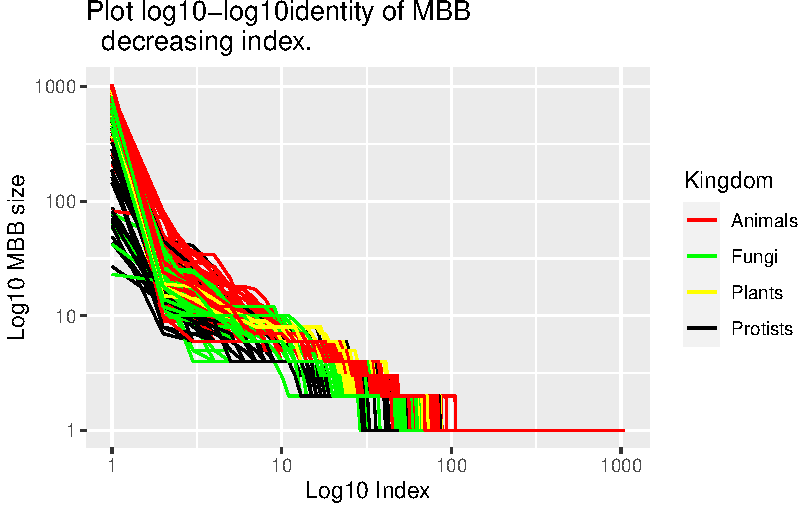
\includegraphics[width=1\textwidth,height=\textheight]{index_files/figure-pdf/unnamed-chunk-52-2.pdf}

}

\end{figure}

\begin{Shaded}
\begin{Highlighting}[]
\NormalTok{p2}
\end{Highlighting}
\end{Shaded}

\begin{figure}[H]

{\centering 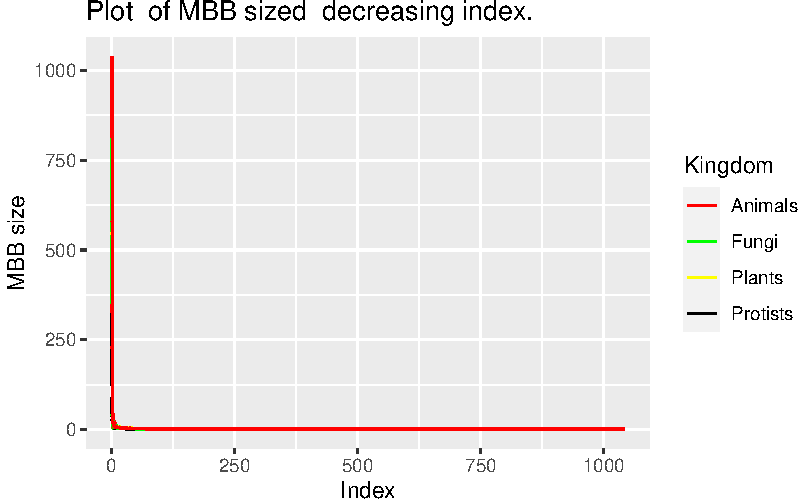
\includegraphics[width=1\textwidth,height=\textheight]{index_files/figure-pdf/unnamed-chunk-52-3.pdf}

}

\end{figure}

\hypertarget{sizes-of-weak-components-for-each-mdag}{%
\subsection{Sizes of weak components for each
mDAG}\label{sizes-of-weak-components-for-each-mdag}}

\begin{Shaded}
\begin{Highlighting}[]
\NormalTok{COLOR\_KINGDOM}\OtherTok{=}\FunctionTok{c}\NormalTok{(}\StringTok{"red"}\NormalTok{,}\StringTok{"yellow"}\NormalTok{,}\StringTok{"green"}\NormalTok{,}\StringTok{"yellow"}\NormalTok{,}\StringTok{"black"}\NormalTok{)}
\NormalTok{colors\_kingdom}\OtherTok{=}\NormalTok{aux2}\SpecialCharTok{\%\textgreater{}\%} \FunctionTok{select}\NormalTok{(Organism,Kingdom) }\SpecialCharTok{\%\textgreater{}\%} \FunctionTok{distinct}\NormalTok{()}
\FunctionTok{names}\NormalTok{(COLOR\_KINGDOM)}\OtherTok{=}\FunctionTok{sort}\NormalTok{(}\FunctionTok{unique}\NormalTok{(colors\_kingdom}\SpecialCharTok{$}\NormalTok{Kingdom))}

\NormalTok{p0}\OtherTok{\textless{}{-}}\FunctionTok{ggplot}\NormalTok{(}\AttributeTok{data=}\NormalTok{aux2) }\SpecialCharTok{+} 
  \FunctionTok{geom\_line}\NormalTok{(}\AttributeTok{mapping=}\FunctionTok{aes}\NormalTok{(}\AttributeTok{x=}\NormalTok{index,}\AttributeTok{y=}\NormalTok{csize,}\AttributeTok{group =}\NormalTok{ Organism,}\AttributeTok{color=}\NormalTok{Kingdom),}\AttributeTok{na.rm=}\ConstantTok{TRUE}\NormalTok{) }\SpecialCharTok{+} 
  \FunctionTok{scale\_x\_continuous}\NormalTok{(}\AttributeTok{trans=}\StringTok{\textquotesingle{}log10\textquotesingle{}}\NormalTok{) }\SpecialCharTok{+} 
  \FunctionTok{scale\_y\_continuous}\NormalTok{(}\AttributeTok{trans=}\StringTok{\textquotesingle{}identity\textquotesingle{}}\NormalTok{) }\SpecialCharTok{+}
  \FunctionTok{scale\_color\_manual}\NormalTok{(}\AttributeTok{values =}\NormalTok{COLOR\_KINGDOM[colors\_kingdom}\SpecialCharTok{$}\NormalTok{Kingdom])}\SpecialCharTok{+}
   \FunctionTok{ggtitle}\NormalTok{(}\StringTok{"Plot log{-}identity of size  weak components decreasing index."}\NormalTok{) }\SpecialCharTok{+}
  \FunctionTok{ylab}\NormalTok{(}\StringTok{"Log10 Weak componente size"}\NormalTok{) }\SpecialCharTok{+} \FunctionTok{xlab}\NormalTok{(}\StringTok{"Index"}\NormalTok{)}


\NormalTok{p1}\OtherTok{\textless{}{-}} \FunctionTok{ggplot}\NormalTok{(}\AttributeTok{data=}\NormalTok{aux2) }\SpecialCharTok{+} 
  \FunctionTok{geom\_line}\NormalTok{(}\AttributeTok{mapping=}\FunctionTok{aes}\NormalTok{(}\AttributeTok{x=}\NormalTok{index,}\AttributeTok{y=}\NormalTok{csize,}\AttributeTok{group =}\NormalTok{ Organism,}\AttributeTok{color=}\NormalTok{Kingdom),}\AttributeTok{na.rm=}\ConstantTok{TRUE}\NormalTok{) }\SpecialCharTok{+} 
  \FunctionTok{scale\_y\_continuous}\NormalTok{(}\AttributeTok{trans=}\StringTok{\textquotesingle{}log10\textquotesingle{}}\NormalTok{) }\SpecialCharTok{+} 
  \FunctionTok{scale\_x\_continuous}\NormalTok{(}\AttributeTok{trans=}\StringTok{\textquotesingle{}log10\textquotesingle{}}\NormalTok{) }\SpecialCharTok{+}
  \FunctionTok{scale\_color\_manual}\NormalTok{(}\AttributeTok{values =}\NormalTok{COLOR\_KINGDOM[colors\_kingdom}\SpecialCharTok{$}\NormalTok{Kingdom])}\SpecialCharTok{+}
   \FunctionTok{ggtitle}\NormalTok{(}\StringTok{"Plot log{-}log of size  weak components decreasing index."}\NormalTok{) }\SpecialCharTok{+}
  \FunctionTok{ylab}\NormalTok{(}\StringTok{"Log10 weak component size"}\NormalTok{) }\SpecialCharTok{+} \FunctionTok{xlab}\NormalTok{(}\StringTok{"Log10 Index"}\NormalTok{)}

\NormalTok{p2}\OtherTok{\textless{}{-}} \FunctionTok{ggplot}\NormalTok{(}\AttributeTok{data=}\NormalTok{aux2) }\SpecialCharTok{+} 
  \FunctionTok{geom\_line}\NormalTok{(}\AttributeTok{mapping=}\FunctionTok{aes}\NormalTok{(}\AttributeTok{x=}\NormalTok{index,}\AttributeTok{y=}\NormalTok{csize,}\AttributeTok{group =}\NormalTok{ Organism,}\AttributeTok{color=}\NormalTok{Kingdom),}\AttributeTok{na.rm=}\ConstantTok{TRUE}\NormalTok{) }\SpecialCharTok{+} 
   \FunctionTok{scale\_x\_continuous}\NormalTok{(}\AttributeTok{trans=}\StringTok{"identity"}\NormalTok{) }\SpecialCharTok{+} 
  \FunctionTok{scale\_y\_continuous}\NormalTok{(}\AttributeTok{trans=}\StringTok{"identity"}\NormalTok{) }\SpecialCharTok{+}
  \FunctionTok{ylim}\NormalTok{(}\DecValTok{0}\NormalTok{,}\DecValTok{1039}\NormalTok{)}\SpecialCharTok{+}
   \FunctionTok{ggtitle}\NormalTok{(}\StringTok{"Plot  of size  weak components decreasing index."}\NormalTok{)}\SpecialCharTok{+}  \FunctionTok{ylab}\NormalTok{(}\StringTok{"Weak components size"}\NormalTok{) }\SpecialCharTok{+} \FunctionTok{xlab}\NormalTok{(}\StringTok{"Index"}\NormalTok{)}\SpecialCharTok{+}
  \FunctionTok{scale\_color\_manual}\NormalTok{(}\AttributeTok{values =}\NormalTok{COLOR\_KINGDOM[colors\_kingdom}\SpecialCharTok{$}\NormalTok{Kingdom])}


\NormalTok{p0}
\end{Highlighting}
\end{Shaded}

\begin{figure}[H]

{\centering 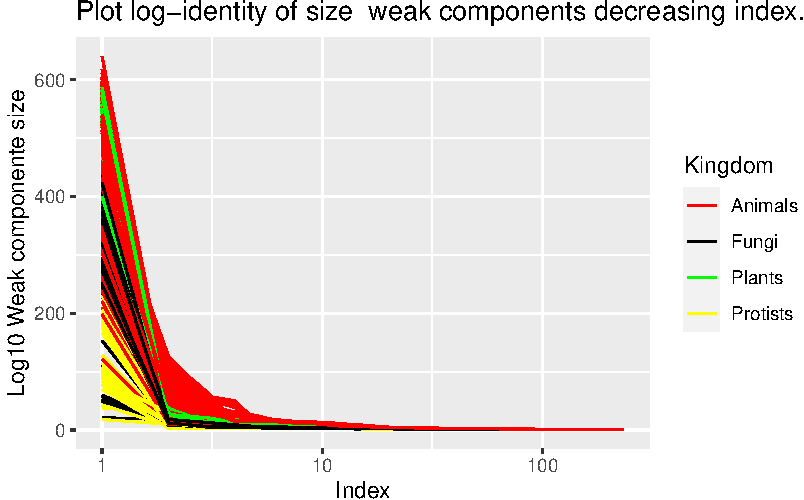
\includegraphics[width=1\textwidth,height=\textheight]{index_files/figure-pdf/unnamed-chunk-53-1.pdf}

}

\end{figure}

\begin{Shaded}
\begin{Highlighting}[]
\NormalTok{p1}
\end{Highlighting}
\end{Shaded}

\begin{figure}[H]

{\centering 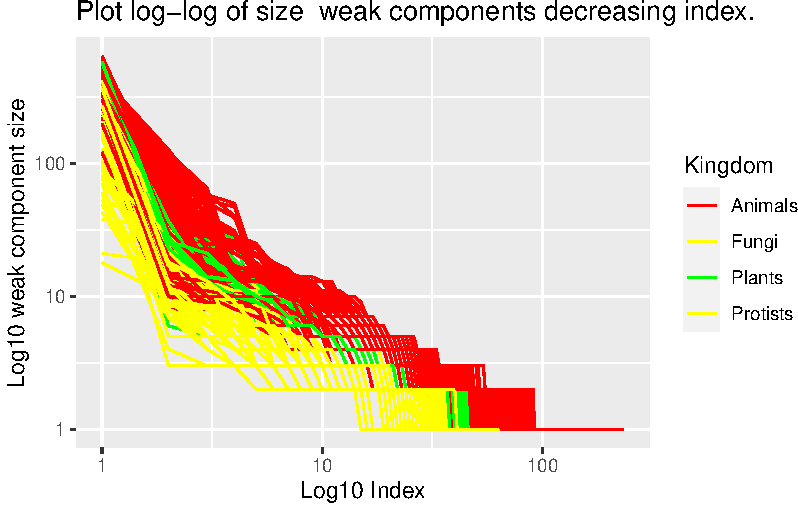
\includegraphics[width=1\textwidth,height=\textheight]{index_files/figure-pdf/unnamed-chunk-53-2.pdf}

}

\end{figure}

\begin{Shaded}
\begin{Highlighting}[]
\NormalTok{p2}
\end{Highlighting}
\end{Shaded}

\begin{figure}[H]

{\centering 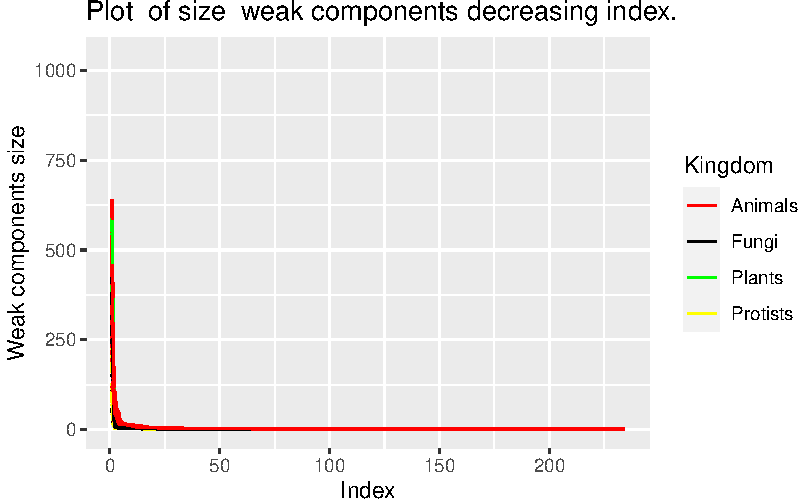
\includegraphics[width=1\textwidth,height=\textheight]{index_files/figure-pdf/unnamed-chunk-53-3.pdf}

}

\end{figure}

\begin{Shaded}
\begin{Highlighting}[]
\NormalTok{data2}\OtherTok{=}\NormalTok{big\_MBB\_list2 }\SpecialCharTok{\%\textgreater{}\%} \FunctionTok{filter}\NormalTok{(index }\SpecialCharTok{\%in\%} \DecValTok{2}\SpecialCharTok{:}\DecValTok{20}\NormalTok{)}
\NormalTok{p3}\OtherTok{\textless{}{-}} \FunctionTok{ggplot}\NormalTok{(}\AttributeTok{data=}\NormalTok{data2) }\SpecialCharTok{+} 
  \FunctionTok{geom\_line}\NormalTok{(}\AttributeTok{mapping=}\FunctionTok{aes}\NormalTok{(}\AttributeTok{x=}\NormalTok{index,}\AttributeTok{y=}\NormalTok{MBBsize,}\AttributeTok{group =}\NormalTok{ Organism,}\AttributeTok{color=}\NormalTok{Kingdom),}\AttributeTok{na.rm=}\ConstantTok{TRUE}\NormalTok{)}\SpecialCharTok{+}
   \FunctionTok{scale\_x\_continuous}\NormalTok{(}\AttributeTok{trans=}\StringTok{"identity"}\NormalTok{) }\SpecialCharTok{+} 
  \FunctionTok{scale\_y\_continuous}\NormalTok{(}\AttributeTok{trans=}\StringTok{"identity"}\NormalTok{) }\SpecialCharTok{+}
  \FunctionTok{ylim}\NormalTok{(}\DecValTok{0}\NormalTok{,}\DecValTok{25}\NormalTok{)}\SpecialCharTok{+}
   \FunctionTok{ggtitle}\NormalTok{(}\StringTok{"Plot  of size  weak components  decreasing index 2 to 20."}\NormalTok{)}\SpecialCharTok{+}  \FunctionTok{ylab}\NormalTok{(}\StringTok{"Weak components size"}\NormalTok{) }\SpecialCharTok{+} \FunctionTok{xlab}\NormalTok{(}\StringTok{"Index"}\NormalTok{)}\SpecialCharTok{+}
  \FunctionTok{scale\_color\_manual}\NormalTok{(}\AttributeTok{values =}\NormalTok{COLOR\_KINGDOM[colors\_kingdom}\SpecialCharTok{$}\NormalTok{Kingdom])}

\NormalTok{p3}
\end{Highlighting}
\end{Shaded}

\begin{figure}[H]

{\centering 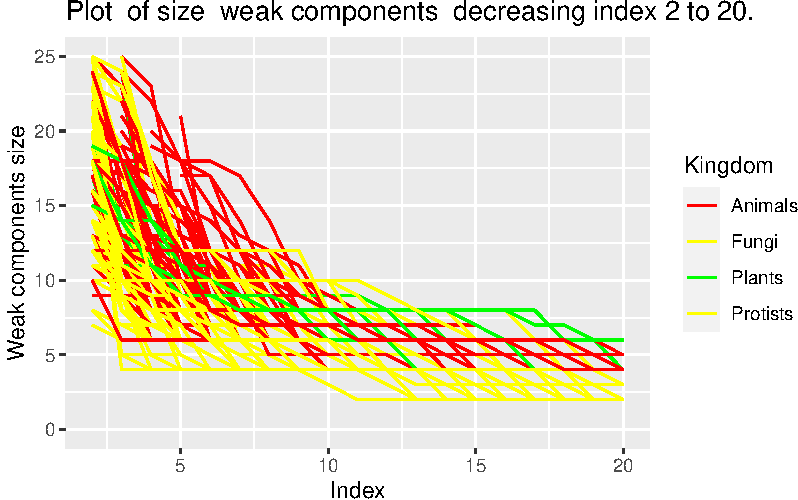
\includegraphics[width=1\textwidth,height=\textheight]{index_files/figure-pdf/unnamed-chunk-54-1.pdf}

}

\end{figure}



\end{document}
